\documentclass[11pt,reqno]{amsart}
%% preamble.tex
\usepackage[T1]{fontenc}
\usepackage[utf8]{inputenc}
\usepackage{lmodern}
\usepackage[letterpaper,left=1.3in,right=1.3in,top=1.15in,bottom=1.15in,
  footskip=0.45in]{geometry}
\usepackage{amsmath,amssymb,amsthm,mathrsfs}
\usepackage{mathtools}
\usepackage[dvipsnames]{xcolor}
\usepackage{graphicx}
\usepackage{tikz}
\usetikzlibrary{arrows.meta,calc,positioning,decorations.pathmorphing,
  patterns,shapes.geometric,matrix,fit,backgrounds}
\usepackage{enumitem}
\usepackage{booktabs}
\usepackage{longtable}
\usepackage{array}
\usepackage{placeins}
\usepackage{microtype}
\usepackage[colorlinks=true,linkcolor=DeepBlue,citecolor=DeepBlue,
  urlcolor=DeepBlue,breaklinks=true]{hyperref}
\usepackage[capitalize,nameinlink]{cleveref}
\hypersetup{pdftitle={Algebraic Loci of Weil Classes on Abelian
  Varieties},
  pdfauthor={Deep Bhattacharjee, Priyabrata Mandal and Ushashi Bhattacharya},
  pdfkeywords={Hodge conjecture, Weil classes, abelian varieties}}

\definecolor{DeepBlue}{RGB}{0,0,139}
\setlength{\emergencystretch}{3em}
\hbadness=3000
\raggedbottom
\interfootnotelinepenalty=0

%% ---------------------------------------------------------------- floats
\renewcommand{\topfraction}{0.92}
\renewcommand{\bottomfraction}{0.75}
\renewcommand{\textfraction}{0.06}
\renewcommand{\floatpagefraction}{0.72}

%% ---------------------------------------------------------- theorem envs
\theoremstyle{plain}
\newtheorem{theorem}{Theorem}[section]
\newtheorem{lemma}[theorem]{Lemma}
\newtheorem{proposition}[theorem]{Proposition}
\newtheorem{corollary}[theorem]{Corollary}
\newtheorem{conjecture}[theorem]{Conjecture}

\theoremstyle{definition}
\newtheorem{definition}[theorem]{Definition}
\newtheorem{example}[theorem]{Example}
\newtheorem{setupenv}[theorem]{Setup}
\newtheorem{question}[theorem]{Question}

\theoremstyle{remark}
\newtheorem{remark}[theorem]{Remark}
\newtheorem{notation}[theorem]{Notation}

\renewcommand{\qedsymbol}{$\blacksquare$}

\crefname{setupenv}{Setup}{Setups}
\crefname{part}{Part}{Parts}
\Crefname{part}{Part}{Parts}
\Crefname{setupenv}{Setup}{Setups}

%% ------------------------------------------------------------- notation
\newcommand{\QQ}{\mathbb{Q}}
\newcommand{\ZZ}{\mathbb{Z}}
\newcommand{\RR}{\mathbb{R}}
\newcommand{\CC}{\mathbb{C}}
\newcommand{\PP}{\mathbb{P}}
\newcommand{\NN}{\mathbb{N}}
\newcommand{\Av}{A^{\vee}}
\newcommand{\cP}{\mathcal{P}}
\newcommand{\cF}{\mathcal{F}}
\newcommand{\cE}{\mathcal{E}}
\newcommand{\cG}{\mathcal{G}}
\newcommand{\cO}{\mathcal{O}}
\newcommand{\cL}{\mathcal{L}}
\newcommand{\cH}{\mathcal{H}}
\newcommand{\cI}{\mathcal{I}}
\newcommand{\cK}{\mathcal{K}}
\newcommand{\cA}{\mathcal{A}}
\newcommand{\cD}{\mathcal{D}}
\newcommand{\cV}{\mathcal{V}}
\newcommand{\cS}{\mathcal{S}}
\newcommand{\cX}{\mathcal{X}}
\newcommand{\cZ}{\mathcal{Z}}
\newcommand{\cQ}{\mathcal{Q}}
\newcommand{\Hdg}{\mathrm{Hdg}}
\newcommand{\HW}{W}                      % the Weil line
\newcommand{\NS}{\mathrm{NS}}
\newcommand{\Nm}{\mathrm{N}}             % the norm character
\newcommand{\cl}{\mathrm{cl}}
\newcommand{\Cn}{\mathrm{Cn}}
\newcommand{\bpf}{\mathrm{bpf}}

\DeclareMathOperator{\CH}{CH}
\DeclareMathOperator{\ch}{ch}
\DeclareMathOperator{\td}{td}
\DeclareMathOperator{\rk}{rk}
\DeclareMathOperator{\End}{End}
\DeclareMathOperator{\Hom}{Hom}
\DeclareMathOperator{\Ext}{Ext}
\DeclareMathOperator{\Pic}{Pic}
\DeclareMathOperator{\Hilb}{Hilb}
\DeclareMathOperator{\Res}{Res}
\DeclareMathOperator{\MT}{MT}
\DeclareMathOperator{\Hg}{Hg}
\DeclareMathOperator{\Gal}{Gal}
\DeclareMathOperator{\coker}{coker}
\DeclareMathOperator{\image}{im}
\DeclareMathOperator{\id}{id}
\DeclareMathOperator{\Spec}{Spec}
\DeclareMathOperator{\Supp}{Supp}
\DeclareMathOperator{\codim}{codim}
\DeclareMathOperator{\Sec}{Sec}
\DeclareMathOperator{\Tr}{Tr}
\DeclareMathOperator{\GU}{GU}
\DeclareMathOperator{\GL}{GL}
\DeclareMathOperator{\SL}{SL}
\DeclareMathOperator{\SU}{SU}
\DeclareMathOperator{\SO}{SO}
\DeclareMathOperator{\Sp}{Sp}
\DeclareMathOperator*{\colim}{colim}
\DeclareMathOperator{\ob}{ob}
\DeclareMathOperator{\Ann}{Ann}

\newcommand{\weightlattice}{\Lambda}
\newcommand{\Kx}{K^{\times}}
\newcommand{\bbar}[1]{\overline{#1}}
\allowdisplaybreaks[2]

\graphicspath{{figures/}}

\title[Algebraic loci of Weil classes]
      {Algebraic Loci of Weil Classes on Abelian Varieties}

\author{Deep Bhattacharjee\textsuperscript{\dag}}
\address{Formerly, Electro-Gravitational Space Propulsion Laboratory (EGSPL),
  Bhubaneswar, Odisha 751030, India}
\email{d.bhattacharjee@erl-forschung.de}
\email{itsdeep@live.com}
\urladdr{\textnormal{ORCID
  \href{https://orcid.org/0000-0003-0466-750X}{0000-0003-0466-750X}}}

\author{Priyabrata Mandal}
\address{Department of Mathematics, Bioinformatics and Computer
  Applications, Maulana Azad National Institute of Technology Bhopal,
  Bhopal 462003, India}
\email{priyabrata@manit.ac.in}
\urladdr{\textnormal{ORCID
  \href{https://orcid.org/0000-0001-6472-6239}{0000-0001-6472-6239}}}

\author{Ushashi Bhattacharya}
\address{Formerly, National Taiwan University, Taipei 106319, Taiwan}
\email{rai.bhattacharya.in@gmail.com}
\urladdr{\textnormal{ORCID
  \href{https://orcid.org/0009-0002-2254-3914}{0009-0002-2254-3914}}}

\thanks{\textsuperscript{\dag}\,Corresponding author: Deep Bhattacharjee,
\texttt{d.bhattacharjee@erl-forschung.de}, \texttt{itsdeep@live.com}.}

\thanks{An earlier preprint by the first and third authors, \emph{Relative
secant cycles and Hodge classes}, Preprints.org (2026),
\href{https://doi.org/10.20944/preprints202602.0462.v5}{\texttt{doi:10.20944/preprints202602.0462.v5}},
contains errors and incomplete proofs and is replaced by the present paper;
Priyabrata Mandal was not an author of it, and Ushashi Bhattacharya was its
second author.}

\thanks{Every proof is given in the text. Programs that repeat much of the
finite arithmetic, and a Lean~4 certificate of part of it, are archived as
described in the statement on data availability at the end of the paper; no
statement rests on them.}


\date{\today}

\subjclass[2020]{Primary 14C30 (Hodge theory), 14C25 (algebraic cycles);
  Secondary 14K05 (algebraic theory of abelian varieties), 14K22 (complex
  multiplication), 14K20 (analytic theory of abelian varieties), 14D07
  (variation of Hodge structures), 14D05 (monodromy of families), 14G35
  (Shimura varieties), 14F08 (derived categories of sheaves), 14M10 (complete
  intersections), 14J70 (hypersurfaces), 14H45 (special curves), 14J28 (K3
  surfaces), 11G10 (abelian varieties of dimension greater than one), 32G20
  (period matrices), 13D07 (homological functors on modules), 32U40
  (currents), 49Q15 (integral currents), 03B35 (mechanization of proofs)}

\keywords{Hodge conjecture, Weil classes, abelian varieties}

\begin{document}

\begin{abstract}
We prove that in every family of abelian varieties of Weil type, for every CM
field, dimension and discriminant, the Weil classes are algebraic on a dense
set that contains an explicit CM point and is either the whole family or
meagre, that every rational Hodge class is algebraic on the very general
complete intersection of diagonal quadrics of Vandermonde type and on every
smooth complete intersection of two diagonal cubics, quartics or sextics in
$\PP^{6}$, and, taking theorems of recent unrefereed preprints as
hypotheses, that the Weil classes are algebraic on every abelian sixfold of
Weil type and the Hodge conjecture holds on every power of the Kuga--Satake
variety of a K3 surface, in particular of a Mumford fourfold.
\end{abstract}

\maketitle

\setcounter{tocdepth}{0}
\vspace*{-18pt}
\begingroup
\setlength{\parskip}{0pt}
\tableofcontents
\endgroup
\vspace*{-4pt}

\section{Introduction}\label{sec:intro}
\addcontentsline{toc}{part}{\protect\tocpart{}{}{Introduction}}

Let $X$ be a smooth complex projective variety. The Hodge conjecture asserts
that the cycle class map
\[
  \cl^{p}_{X}\colon \CH^{p}(X)_{\QQ}\longrightarrow \Hdg^{p}(X)
  \coloneqq H^{2p}(X,\QQ)\cap H^{p,p}(X)
\]
is surjective for every $p$. For $p=1$ this is the theorem of Lefschetz on
$(1,1)$ classes.%
\footnote{The rational coefficients are essential. The theorem of Lefschetz
holds integrally in degree two, but the integral analogue fails in higher
degree: Atiyah and Hirzebruch found torsion classes of type $(p,p)$ that are
not classes of cycles, and Koll\'ar found non-torsion ones. Every statement in
this paper concerns $\QQ$-coefficients.}
Beyond degree two the best understood Hodge classes are those of abelian
varieties, and the first of them that divisors do not produce are the Weil
classes. Weil exhibited them on abelian varieties with an action of an
imaginary quadratic field whose two eigenspaces on the tangent space have the
same dimension, showed that they are Hodge classes outside the subring
generated by divisor classes, and proposed them as test cases for the Hodge
conjecture \cite{Weil77}. The construction works for every CM field $F$ in
place of the quadratic one. On a general abelian variety of Weil type the
Hodge ring is generated by divisor classes together with the Weil classes, a
flat $F$-line of classes of middle degree, so for these varieties the Hodge
conjecture is the algebraicity of the Weil classes.

Markman proved that the Weil classes are algebraic on the abelian sixfolds of
split Weil type for every imaginary quadratic field, and, through a product
argument of Schoen \cite[Proposition~10]{Sch98}, on every abelian fourfold of
Weil type \cite{Mar25a,Mar25b}.%
\footnote{In the normalisation of \Cref{def:disc} the discriminant is the
class of $(-1)^{n}\det H$ in $\QQ^{\times}_{>0}/\Nm_{K/\QQ}(K^{\times})$.
Markman uses the class of $\det H$ itself, in which the same sixfolds have
discriminant $(-1)^{3}=-1$.}
With the description of the Hodge rings of abelian varieties of dimension at
most five by Moonen and Zarhin \cite{MZ99}, this gives the Hodge conjecture
for abelian fourfolds and fivefolds. His sheaves are built from secant sheaves
on an abelian variety of half the dimension, and they extend along the family
because they satisfy an equivariant form of semiregularity. This paper is
about what can be proved for every CM field and every dimension at once.

\subsection{The main theorem}

Fix a CM field $F$ of degree $2m$, an integer $n\ge2$ and a discriminant
$\delta$. The abelian varieties of $(F,n,\delta)$-Weil type are the members of
one family over a connected period domain $\cD_{F}$ of dimension $mn^{2}$, a
product of $m$ copies of the bounded symmetric domain of $\SU(n,n)$, and their
Weil classes form a flat local system of rank $2m$ over it
(\Cref{setup:cmfield}, \Cref{prop:cmweil}). We call the set
\[
  \Sigma_{F}=\{\,s\in\cD_{F}:\text{the Weil classes of }A_{s}\text{ are
  algebraic}\,\}
\]
the \emph{algebraic locus} of the family. A property holds for the
\emph{very general member} if it holds outside a countable union of proper
closed analytic subsets of $\cD_{F}$.%
\footnote{A subset of $\cD_{F}$ is \emph{meagre} if it is contained in a
countable union of closed subsets with empty interior. Since $\cD_{F}$ is a
complex manifold, the Baire category theorem shows that a meagre set has
dense complement, so a statement that holds off a meagre set holds on a dense
set of members; the very general members are those off a particular meagre
set, a countable union of proper analytic subsets.}

\begin{theorem}[Main theorem]\label{thm:main}
For every CM field $F$, every $n\ge2$ and every discriminant $\delta$, the
algebraic locus $\Sigma_{F}$ of the Weil classes has the following
properties.
\begin{enumerate}[label=\textup{(\roman*)},leftmargin=2.6em,itemsep=2pt]
\item It contains an explicit point $s_{0}$ at which $A_{s_{0}}$ is isogenous
  to a product of abelian varieties with complex multiplication by $F$, and
  at which the Weil classes are polynomials with rational coefficients in
  divisor classes.
\item It is dense in $\cD_{F}$.%
\footnote{Density comes from the Hecke orbit of $s_{0}$: the group
$G_{F}(\QQ)$ of rational points of the unitary group of the hermitian form
acts on $\cD_{F}$ through isogenies that respect the $F$-action and the
polarisation up to a scalar, so it preserves the algebraicity of the Weil
classes, and the closure of $G_{F}(\QQ)$ contains the identity component of
$G_{F}(\RR)$, which acts transitively on $\cD_{F}$; the proof uses the
rational isotropic vectors of the hermitian form, which exist by the Hasse
principle.}
\item It is the preimage of a countable union of Zariski closed subsets of the
  Shimura variety of the family, and either $\Sigma_{F}=\cD_{F}$ or
  $\Sigma_{F}$ is meagre.
\item The following are equivalent: $\Sigma_{F}$ is closed; $\Sigma_{F}$ has
  an interior point; the Weil classes are algebraic on every member of the
  family; the Hodge conjecture holds for the very general member of the
  family.
\end{enumerate}
\end{theorem}

For $n=1$ the Weil classes have degree two and are algebraic by the theorem
of Lefschetz, and all four statements hold trivially. The proof of
\Cref{thm:main} is completed in \Cref{sec:cmfields}, after the imaginary
quadratic case has been treated in full in \Cref{part:basepoints}.
\Cref{fig:mainlocus} draws the picture it describes: a connected domain, a
dense set built from one explicit point, and a decomposition of that set into
countably many closed algebraic strata.

The theorem carries the Hodge conjecture for the very general abelian variety
of Weil type, for every CM field, every dimension and every discriminant, to
a single topological statement about one explicit set: the dense set
$\Sigma_{F}$, which is a countable union of closed algebraic subsets of a
connected Shimura variety, has to be closed. The rest of the paper is
organised around that statement. \Cref{part:obstructions} shows why the
classical constructions do not produce Weil classes and fixes the explicit
form of the classes; \Cref{part:basepoints} proves the theorem for imaginary
quadratic fields; \Cref{part:semiregularity} determines what closing
$\Sigma_{F}$ requires of a single object at a single point;
\Cref{part:cmfields} completes the proof for every CM field and computes the
requirement exactly for quartic fields; and \Cref{part:beyond} places the
Weil classes inside the whole conjecture (\Cref{fig:parts}).

The paper also proves the Hodge conjecture itself on a family of varieties
of every dimension. Let $X\subset\PP^{N}$ be a complete intersection of $c$
diagonal hypersurfaces $\sum_{i}a_{ki}x_{i}^{d}=0$ of degree $d$. It is
\emph{of Vandermonde type} if $a_{ki}=\mu_{i}\sum_{l=1}^{c}g_{kl}\lambda_{i}^{l-1}$
for distinct numbers $\lambda_{0},\dots,\lambda_{N}$, nonzero numbers
$\mu_{i}$ and an invertible matrix $(g_{kl})$; for $c\ge2$ this says that the
columns of $(a_{ki})$ are distinct points of a rational normal curve, and
every smooth complete intersection of two diagonal hypersurfaces of the same
degree is of this type. Such an $X$ is isomorphic to a variety
$X_{d,N-c}(\lambda)$ that depends only on $\lambda$ (\Cref{thm:vandermonde}),
and \emph{very general} refers to $\lambda$. For $d=2$ we call $X$ a
\emph{Vandermonde quadric intersection}.

\begin{theorem}[Diagonal complete intersections]\label{thm:introvandermonde}
Every rational Hodge class is algebraic on the very general Vandermonde
quadric intersection, in every dimension and in every projective space. The
same holds for the very general complete intersection of Vandermonde type of
diagonal cubics or quartics of dimension at most seven, or of diagonal
sextics of dimension at most five, and for every smooth complete
intersection of two diagonal cubics, of two diagonal quartics or of two
diagonal sextics in $\PP^{6}$.
\end{theorem}

The first two statements are \Cref{thm:vgvandermonde}(iii) and the third is
\Cref{cor:twodiagonal}(ii). The variety $X$ is a quotient of a power of a
generalised Fermat curve, so its Hodge classes come from abelian subvarieties
of the Jacobian of that curve. For quadrics the monodromy of the curve along
a chain of vanishing cycles is the full symplectic group on every eigenspace,
so every Hodge class comes from powers of polarisations and no theorem on
abelian varieties of higher dimension is needed. For cubics, quartics and
sextics we compute the monodromy by an induction on the number of branch
points (\Cref{prop:cyclicmonodromy}), and the classes it leaves are divisor
classes, Weil classes of abelian fourfolds of Weil type, and Weil classes of
abelian sixfolds of split Weil type, all algebraic by the theorems of
Lefschetz and Markman \cite{Mar25a,Mar25b}. In odd dimension every Hodge
class is a multiple of a power of the hyperplane class. So the bound seven
for cubics and quartics is the point where abelian varieties of dimension
eight appear, and the bound five for sextics comes from abelian sixfolds of
non-split Weil type, which occur in dimension six. Taking the theorems of
the preprints discussed below as hypotheses, these bounds rise to nine and
seven (\Cref{thm:weilsix}), and the Hodge conjecture holds on every power of
the very general member in every degree (\Cref{cor:vgalldegrees}); for one
or two equations that last statement is a theorem of \cite{OAI26a}, proved
there independently.

\begin{figure}[htbp]
\centering
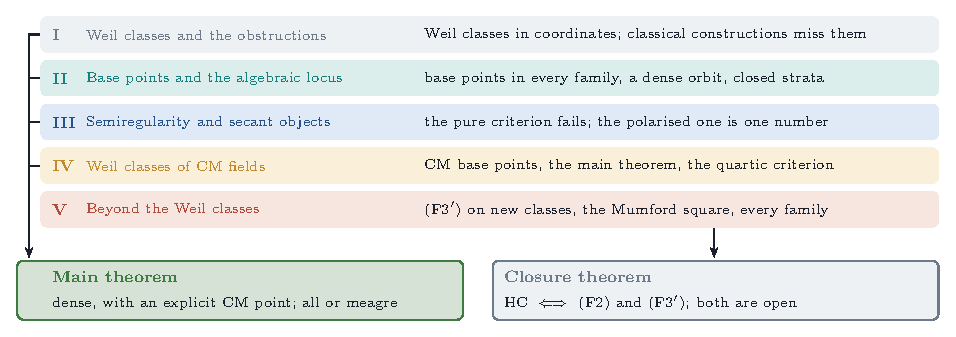
\includegraphics[width=\textwidth]{fig_roadmap}
\caption{The five parts of the paper. Parts I to IV lead to
\Cref{thm:main}; all five lead to the closure theorem of
\Cref{sec:final}, by which the Hodge conjecture is equivalent to the two
statements (F2) and (F3$'$), both of which remain open.}
\label{fig:parts}
\end{figure}

\begin{figure}[htbp]
\centering
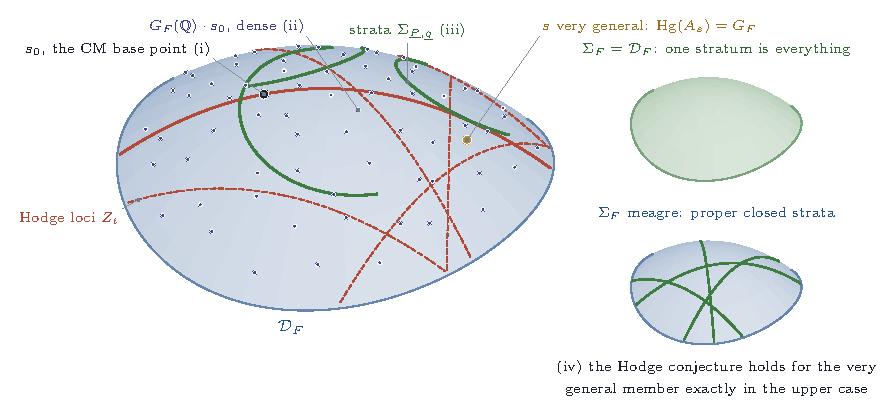
\includegraphics[width=\textwidth]{fig_mainlocus}
\caption{The algebraic locus of \Cref{thm:main}, drawn over a real slice of the
period domain $\cD_{F}$. Left: the explicit CM base point $s_{0}$ of part (i);
its Hecke orbit $G_{F}(\QQ)\cdot s_{0}$, which is dense by part (ii); three of
the strata $\Sigma_{\underline{P},\underline{q}}$ of part (iii), each closed
and algebraic, through points of the orbit; the Hodge loci $Z_{t}$, dashed,
one of them through $s_{0}$, off which the Hodge group of the member is all of
$G_{F}$ (\Cref{lem:cmgeneric}); and a very general point $s$. Right: the two
cases of the dichotomy of part (iii). By part (iv) the Hodge conjecture holds
for the very general member exactly in the upper case, where one stratum is
the whole domain.}
\label{fig:mainlocus}
\end{figure}

\subsection{The proof}

The first step is a base point. In \Cref{thm:cmbasepoint} the member $A_{s_{0}}$
is isogenous to $B_{\Phi}^{\,n}\times B_{\bbar\Phi}^{\,n}$, where $B_{\Phi}$ is
an abelian $m$-fold with complex multiplication by $F$ of a CM type determined
by the polarisation, and the Weil classes there are written out as
polynomials with rational coefficients in $F$-balanced divisor classes. For
an imaginary quadratic field $K$ there is a second base point in every family,
with quaternionic multiplication: whenever an algebra $(-d,b)_{\QQ}$ with
$b>0$ acts compatibly with $K$, the Weil line is spanned by the real and
imaginary parts of $\Theta^{n}$ for an explicit $(1,1)$ class $\Theta$, and
the discriminant of the family is the class of $b^{n}$, which can be any
discriminant (\Cref{thm:divcriterion}, \Cref{thm:quatweil},
\Cref{thm:everyfamily}). Products of abelian surfaces of Weil type give a
third, since the Weil class is multiplicative:
$\omega(A_{1})\,\omega(A_{2})=\omega(A_{1}\times A_{2})$ for the
$K$-valued Weil class $\omega$ (\Cref{thm:weilmult}, \Cref{thm:everyn}). None
of these base points uses anything beyond the theorem of Lefschetz on $(1,1)$
classes.

The second step moves the base point. An element of $G_{F}(\QQ)$, where
$G_{F}=\Res_{F_{0}/\QQ}\SU(V,H)$ and $F_{0}$ is the totally real subfield,
induces after clearing denominators an isogeny between two members and fixes
the Weil classes, so $\Sigma_{F}$ is a union of $G_{F}(\QQ)$-orbits
(\Cref{lem:Ginvariance}). The hermitian form is isotropic by the Hasse
principle, the rational points of the unipotent radicals of the parabolic
subgroups are dense in their real points, and these real points generate the
identity component of $G_{F}(\RR)$; so every orbit is dense
(\Cref{prop:densealg}, \Cref{thm:cmpropagation}(ii)).

The third step is properness. The relative Hilbert scheme of the universal
family, for one tuple of Hilbert polynomials, is proper over the Shimura
variety,%
\footnote{By Grothendieck's construction the Hilbert scheme of a projective
morphism, for a fixed Hilbert polynomial, is projective over the base; here
the base is the Shimura variety of the family, after a level structure that
makes the universal family exist, and the morphism is the universal abelian
scheme.}
and the class of a flat family of cycles is locally constant, so the
set of points at which a Weil class is represented by cycles with prescribed
Hilbert data is Zariski closed; $\Sigma_{F}$ is the countable union of these
strata (\Cref{thm:closedlocus}). The Baire category theorem then gives the
dichotomy of part (iii) (\Cref{cor:allornothing}). Part (iv) needs one more
fact, that the very general member has Hodge group $G_{F}$; we prove it
directly, from the simplicity of the real factors $\SU(n,n)$
(\Cref{lem:cmgeneric}, \Cref{cor:verygeneral}).

For an imaginary quadratic field everything can be written in coordinates.
On the standard model of \Cref{sec:explicit}, built from a $K$-vector space of
dimension $2n$ with a hermitian form of signature $(n,n)$, the Weil line has
the integral basis
\[
  \omega_{1}=\sum_{|T|\ \mathrm{even}}(-1)^{|T|/2}d^{\,n-|T|/2}\,w^{(T)},
  \qquad
  \omega_{2}=\sum_{|T|\ \mathrm{odd}}(-1)^{(|T|-1)/2}d^{\,n-(|T|+1)/2}\,w^{(T)},
\]
where $T$ runs over the subsets of $\{1,\dots,2n\}$ and $w^{(T)}$ is the
monomial taking $y_{j}$ for $j\in T$ and $x_{j}$ otherwise
(\Cref{thm:explicitgens}). A member with Hodge group $\SU(V,H)$ has exactly
three Hodge classes in degree $2n$ and one in every other degree
(\Cref{thm:hdgcount}), so the Hodge conjecture for it, in every degree at
once, is the algebraicity of the one class $\omega_{1}$, with $2^{2n-1}$
integer coefficients (\Cref{cor:whatisleft}). By Deligne's theorem
\cite{Del82} that class is absolutely Hodge at every point,%
\footnote{A class is absolutely Hodge if its image under every automorphism
$\sigma$ of $\CC$, through the comparison of Betti cohomology with
algebraic de Rham cohomology of the conjugate variety $X^{\sigma}$, is again
a Hodge class. Algebraic classes have this property, so it is a necessary
condition for algebraicity; Deligne proved it for every Hodge class on an
abelian variety.}
and the Hodge
conjecture for the family is equivalent to its algebraicity at every point of
one connected domain (\Cref{cor:exactform}).

\subsection{Closing the algebraic locus}

\enlargethispage{2pt}By \Cref{thm:main}(iv) the Hodge conjecture for the very general member of a
Weil family is the closedness of $\Sigma_{F}$, and by (iii) it is enough to
show that one stratum has an interior point. Two statements would do this,
and the paper determines what each of them asks.

The first bounds the Hilbert data. If at every point of the orbit of the
base point the Weil class is represented by a cycle whose Hilbert data comes
from one finite set, then finitely many strata cover a dense set and one of
them is everything (\Cref{thm:degreebound}). Read on an arbitrary
representative this bound is equivalent to its conclusion
(\Cref{thm:p1equivalent}); read on the transported cycle, the one
representative that can be named, it fails, because the transport multiplies
the degree of a component by $c^{2n}$ and divides it only by the order of a
stabiliser (\Cref{thm:p1forces}). So the bound restates the problem rather
than reducing it.
The bound is needed only on a small set: by the theorem of Pila, Shankar
and Tsimerman on the Andr\'e--Oort conjecture \cite{PST},%
\footnote{In the form used here: an irreducible closed subvariety of a
Shimura variety of abelian type that contains a Zariski dense set of CM
points is a special subvariety. Hence a sequence of CM points that leaves
every proper special subvariety is Zariski dense, and so is every infinite
subsequence of it.}
it suffices along
one sequence of CM points that leaves every proper special subvariety, and
such a sequence exists inside the orbit (\Cref{thm:escape}). Every
member at which this paper exhibits algebraic Weil classes has endomorphisms
beyond the field, so it lies in the locus of members with smaller Hodge
group. That locus contains the base point, is dense, is stable under
$G_{F}(\QQ)$ and is a countable union of closed algebraic strata, exactly as
$\Sigma_{F}$ is, and it is meagre (\Cref{prop:speciallocus},
\Cref{cor:speciallocus}). The properties listed in \Cref{thm:main} therefore
do not decide the dichotomy by themselves, and a proof that $\Sigma_{F}$ is
everything has to reach a member with full Hodge group.

The second is semiregularity. By the theorem of Buchweitz and Flenner, in the
form of Pridham for perfect complexes \cite{BF03,Pri24},%
\footnote{The semiregularity map of a perfect complex $E$ on $X$ sends
$\Ext^{2}(E,E)$ to $\bigoplus_{q}H^{q+2}(X,\Omega^{q}_{X})$ by the trace of
the product with powers of the Atiyah class of $E$; it carries the
obstruction to deforming $E$ along a first order deformation of $X$ to the
obstruction to keeping $\ch(E)$ of Hodge type. If it is injective, $E$
deforms, formally and then along the whole family, in every direction in
which $\ch(E)$ stays a Hodge class. Bloch introduced it for local complete
intersection subvarieties.}
a perfect complex at
one base point whose Chern character is a nonzero multiple of a Weil class
plus a polynomial in the polarisation, and whose semiregularity map is
injective, extends along the whole family and makes $\Sigma_{F}$ everything
(\Cref{thm:semiregclosure}, \Cref{thm:cmpropagation}(v)). The paper computes
the injectivity condition exactly. The annihilator of the Weil class in
$H^{0,2}$ is carried by the polarisation isomorphically onto the tangent space
of the family (\Cref{lem:annihilator}, \Cref{thm:anntangent}), so no object
whose Chern character lies on the Weil line and on which $H^{2}(\cO_{A})$ acts
faithfully is semiregular (\Cref{thm:rankzero}). When the Chern character is
exactly a Weil class the criterion is never met, for any CM field and any
$n\ge2$: a semiregular object would extend to the very general Weil torus of
the field, a complex torus that is not algebraic, on which every coherent
sheaf has vanishing Chern character strictly between degree zero and the top
degree (\Cref{prop:weiltorussheaves}, \Cref{thm:p2false},
\Cref{thm:cmpurefalse}). With powers of the polarisation added the criterion
becomes one number: for a Chern character $N\omega+\sum_{k}c_{k}\theta^{k}$
and $n\ge3$ every object has $\dim\Ext^{2}(E,E)\ge(4+\rho)n^{2}-2n$, where
$\rho\le3$ is the rank of the Hankel matrix of the numbers $k!\,c_{k}$, and
an object attaining this bound meets the criterion
(\Cref{thm:p2primenumber}).%
\footnote{That is, $\rho$ is the rank of the $(2n-1)\times3$ matrix with
entries $\mu_{i+j}$, $0\le j\le2n-2$, $0\le i\le2$, where $\mu_{k}=k!\,c_{k}$
(\Cref{setup:p2prime}). A vector in its kernel is a linear recurrence of order
at most two among the $\mu_{k}$, and $\rho$ does not change when the character
is multiplied by $e^{t\theta}$.}
A flatness condition on the deformations of the object suffices in place of
injectivity (\Cref{prop:p2flat}). By descent and scalar extension the
statement is needed only for the split families of the CM fields of degree at
least four (\Cref{prop:descent}), and for one family it is equivalent to the
Lefschetz standard conjecture for the total space of the family over a curve
through a base point (\Cref{cor:weilequiv}).

For a quartic CM field and $n=2$ we compute the rank exactly for every
shape. It takes fifteen values; the least, $80$, is taken only by the pure
shape, which the Weil tori exclude, so an object meeting the criterion has
$\dim\Ext^{2}(E,E)\ge88$ and a polynomial part that is exponential or linear
at each real place (\Cref{thm:quarticrank}, \Cref{cor:quarticleast}). The
Hodge locus of every such character is determined: it is the Weil tori of the
field only for the characters of $\theta^{4}$ shape, which are therefore
excluded at rank $88$, and the polarised family itself for every other
character of that rank (\Cref{prop:quarticlocus}, \Cref{cor:quarticlocus}).

\subsection{Secant objects}

The objects that a secant construction supplies are examined in
\Cref{sec:secantobjects}. On the split member $X\times\widehat{X}$ of
\Cref{sec:construction} the secant plane is written down in every dimension,
and a secant sheaf has rank $a$, $c_{1}=bt$, $c_{2}=\tfrac{ad+b^{2}}{2}t^{2}$
and Bogomolov discriminant $\Nm_{K/\QQ}(b+a\sqrt{-d})\,t^{2}$
(\Cref{thm:plane}, \Cref{thm:secantexists}). No object whose Chern character
is an effective combination of exponentials of divisor classes contributes to
the Weil line, by a positivity argument with the norm form
(\Cref{thm:positivity}), and no object with a line bundle summand off the
polarisation line meets the criterion, so no sum of line bundles does in any
dimension (\Cref{thm:linebundle}, \Cref{cor:noline}). Convolutions of line
bundles, their iterated cones, are cut down by the maps between the pieces.
Fewer than $2n$ pieces with nondegenerate differences never meet the
criterion (\Cref{thm:fewpieces}). On $E_{0}^{2n}$, $E_{0}=\CC/\ZZ[i]$, the
signed Chern characters of $2\cdot4^{n-1}$ line bundles add up to a real
Weil class (\Cref{prop:weilpieces}), and with three multiples of the
polarisation no convolution of these pieces meets the criterion at $n=3$
(\Cref{thm:noconvolution}), nor at $n=4$ when the shifts of the pieces lie
in six consecutive values (\Cref{cor:efoursix}). The weakened criterion
of \cite[Question~11.4]{Mar25b} reduces, for the transform of
$\cF\boxtimes\cF$, to the single identity
$\mathrm{At}(\cF)^{2}=-d\Theta^{2}\cdot\id$ for the sheaf $\cF$ on the
fourfold (\Cref{thm:factor}); a local computation at an isolated double point
of the support decides it in the negative for Markman's candidate in
dimension eight (\Cref{thm:candidatefails}), and at a quartic CM field a
curve on which a complex is locally free is tangent to at most one of the two
eigenplanes of the real multiplication, which decides Markman's explicit pair
\cite[Example~11.2.7]{Mar25c} in the same way (\Cref{thm:quarticlocal},
\Cref{cor:markmanquarticfails}).

The supports are constrained as well. A Cohen--Macaulay support carries no
local obstruction, while two smooth branches of codimension two meeting
transversally at a point carry one (\Cref{cor:cmdichotomy}). For a smooth support, a surface $S$ in the
fourfold, Grothendieck--Riemann--Roch fixes every numerical invariant, and the
Bogomolov--Miyaoka--Yau inequality gives $d\le b^{2}$ for the twist
$b\Theta$, which leaves only $d\in\{1,3,5,7\}$ for the twist $3\Theta$ of
Markman's candidate (\Cref{thm:smoothinvariants},
\Cref{cor:fourdiscriminants}). Complete
intersections are excluded for every $b$ and $d$ (\Cref{thm:noci}), two-term
complexes of powers of the polarisation at every rank, twist and
discriminant (\Cref{thm:nosplit}), and a Hilbert--Burch resolution of a
secant support has rank at least two (\Cref{prop:lowrankburch}); the secant
class is an integer combination of classes of line bundles exactly when
$d\equiv15$ or $23\pmod{24}$ (\Cref{thm:lattice}).

\subsection{The classical constructions}

\Cref{part:obstructions} explains why two classical lines of attack do not
produce Weil classes, and the explanations are different in kind. The first
imports an object from a projective space, restricts it to the dual abelian
variety and transports it back by the Fourier--Mukai transform. Its Chern
character stays in the subring generated by the polarisation
(\Cref{thm:divisor}), because the cohomological transform carries powers of
the dual polarisation to rational multiples of powers of the polarisation in
closed form (\Cref{thm:fmtheta}); and a construction equivariant for the
field lands in the isotypic component of the norm character, which the Weil
line misses, since it sits at the two ends of the grading
(\Cref{thm:character}). The second is induction on dimension through
hyperplane sections, and the restriction map kills every primitive class of
middle degree (\Cref{thm:hyperplane}); below the middle degree the return
trip is the Lefschetz standard conjecture (\Cref{thm:returntrip}). The
Kuga--Satake construction, which changes the variety rather than cutting it,
reaches the Weil line only in dimension two (\Cref{prop:normpart}).%
\footnote{The construction attaches to a polarised Hodge structure $T$ of
weight two with $h^{2,0}=1$ an abelian variety $A$ with
$H^{1}(A,\QQ)=C^{+}(T)$, the even Clifford algebra, and an embedding of
$T$ into $\End(H^{1}(A,\QQ))$ by Hodge structures, which is a Hodge class on
the product of a variety carrying $T$ with $A\times A$; the Kuga--Satake
Hodge conjecture asks that this class be algebraic.} A rational
class of the Weil line has a $\Kx$-orbit spanning a plane, so any
construction reaching it must be bilinear in a pair of inputs exchanged by
$\Gal(K/\QQ)$ (\Cref{prop:orbitplane}), and Markman's construction is of that
kind.

\subsection{Weil classes and the Hodge conjecture}

\Cref{part:beyond} places the Weil classes inside the conjecture. Two
statements carry all of it. The first, (F2), asks that every Hodge class on an
abelian variety outside the subring generated by divisor classes and Weil
classes of quotients be algebraic; multiplying by an exceptional class on the
square of a Mumford fourfold moves every Hodge class of every abelian variety
outside that subring, so (F2) is equivalent to the Hodge conjecture for all
abelian varieties (\Cref{prop:f2isab}). The second, (F3$'$), asks that every
Hodge class on every smooth projective variety be algebraic modulo the images
of Hodge classes of abelian varieties under algebraic correspondences
(\Cref{def:f3prime}). The Hodge conjecture is equivalent to (F2) and (F3$'$)
together (\Cref{prop:f3prime}, \Cref{thm:final}).

We prove (F3$'$) for every variety whose cohomology is reached from abelian
varieties by correspondences, a class closed under products, surjective
images, blow-ups, projective bundles and Hilbert schemes of points on
surfaces, which contains every Fermat hypersurface and every K3 surface whose
Kuga--Satake correspondence is algebraic (\Cref{prop:f3prime},
\Cref{prop:aclosure}); for every variety of dimension at most three, and on
a variety of dimension $k$ in the degrees $0$, $2$, $2k-2$ and $2k$; for
every fourfold and fivefold whose zero-cycles are supported in dimension at
most three, among them every uniruled fourfold and every rationally connected
fivefold (\Cref{prop:f3primesmall}, \Cref{prop:f3primefibration}); for every
fourfold and fivefold dominated by a variety of that class
(\Cref{prop:f3primedominant}); for every smooth ample divisor of odd
dimension in a variety of that class, and in even dimension outside the
middle degree and for a very general member (\Cref{prop:f3primeample});
and, by a toric compactification whose boundary is again of the same kind, for
every hypersurface of simplex type, so for every smooth Delsarte hypersurface
of every dimension and every cyclic cover branched along one, whose Hodge
conjecture then follows from that of Fermat varieties of one degree
(\Cref{thm:simplextype}, \Cref{cor:delsarteall}). A complete intersection
of diagonal hypersurfaces whose coefficients are of Vandermonde type, which
holds for every smooth complete intersection of two of them, is a quotient
of a power of a generalised Fermat curve, so it satisfies (F3$'$), and its
Hodge conjecture reduces to abelian varieties attached to the characters of
the curve; for two diagonal hypersurfaces of degree $3$, $4$ or $6$ in
$\PP^{6}$ these have dimension at most five, and the Hodge conjecture holds,
the exceptional classes being Weil classes of abelian fourfolds of Weil type
(\Cref{thm:vandermonde}, \Cref{cor:twodiagonal}). At a very general
configuration the monodromy of the curve leaves only the Hodge classes that
come from polarisations and from Weil classes; we compute that monodromy for
cyclic covers of degree three, four and six by an induction on the number of
branch points (\Cref{prop:cyclicmonodromy}), so the Hodge conjecture holds
for the very general such intersection of quadrics in every dimension, of
cubics and quartics up to dimension seven, and of sextics up to dimension
five, in every projective space (\Cref{thm:vgvandermonde}). On the powers, Hilbert
schemes and moduli spaces of a K3 surface whose transcendental field is a CM
field, and on the fourfolds of K3$^{[2]}$ type with field $\QQ$ or a CM
field, the Hodge conjecture itself holds (\Cref{prop:k3powers},
\Cref{prop:k3ntype}).

The first instance of (F2) is a pair of classes on the square of a Mumford
fourfold, and \Cref{sec:beyond} studies it in detail. The two classes are
the real multiplication by a totally real cubic field on the primitive part of
$H^{2}$, and they are algebraic once the Kuga--Satake class of one K3 surface
of Picard number thirteen is algebraic (\Cref{prop:mumfordrm},
\Cref{thm:mumfordks}); they are algebraic at every CM point
(\Cref{thm:mumfordcm}); they are rigid, their Hodge locus being the compact
Mumford curve (\Cref{thm:mumfordrigid}); and they are represented by
algebraic cycles at every closed point of every reduction of the curve modulo
a prime, so that their algebraicity on every member is a bound on the Hilbert
data of those cycles (\Cref{prop:modp}, \Cref{thm:modpdensity}). For an
abelian scheme over a curve whose invariant classes are algebraic the
Lefschetz standard conjecture holds on the total space
(\Cref{thm:lefschetzfamily}), and over a compact Shimura curve the total space
of a Mumford family satisfies the Hodge conjecture
(\Cref{prop:mumfordfivefold}).

The structure that \Cref{thm:main} finds in one family is present in every
family that carries (F2) or (F3$'$) (\Cref{sec:families}). Every Hodge class
of every abelian variety lies in an abelian scheme with a member of CM type,
and (F2) is equivalent to the statement that in every such scheme the
algebraic locus of a flat Hodge class that is algebraic at a CM member has an
interior point (\Cref{prop:cmfamily}, \Cref{thm:f2propagation}); the base
points of the Weil families are the seeds, through Andr\'e's theorem on the
Hodge classes of abelian varieties of CM type. (F3$'$) is equivalent to the
absence of Hodge classes off the part of the cohomology reached from abelian
varieties by algebraic correspondences (\Cref{prop:abpart}). On the squares of
K3 surfaces with real multiplication, where (F3$'$) is first open, the
algebraic locus of the real multiplication contains every CM point, is dense,
is stable under rational Hodge isometries, and is either the whole family or
meagre (\Cref{thm:rmlocus}). In each case the property still missing is the
interior point (\Cref{thm:twostand}).

Seven preprints released by OpenAI in September and October 2026
\cite{OAI26a,OAI26b,OAI26c,OAI26d,OAI26e,OAI26f,OAI26g} announce the Hodge
conjecture for abelian varieties of CM type, the algebraicity of the Weil
classes on the split abelian eightfolds of imaginary quadratic fields and of
the Kuga--Satake class of every K3 surface, the Hodge conjecture for products
of K3 surfaces, and the Hodge conjecture for the powers of Hodge generic
abelian covers of curves and of diagonal hypersurfaces. They have not been
refereed. \Cref{sec:preprints} takes their theorems as hypotheses and
derives, with complete proofs, what they give here: the Weil classes of every
abelian sixfold of Weil type, by a product argument that lowers the dimension
(\Cref{thm:weilsix}); the Hodge conjecture on every power of the
Kuga--Satake variety of a K3 surface, through a spanning lemma for Clifford
algebras, and so on every power of a Mumford fourfold (\Cref{thm:kspowers},
\Cref{cor:mumfordall}); every K3 surface in the class of varieties reached
from abelian varieties, and the
fourfolds of K3$^{[2]}$ type whose N\'eron--Severi space is isotropic or
represents $-2$, as when the Picard number is at least four
(\Cref{cor:k3all}, \Cref{prop:k3twosmall}); the Hodge conjecture
on every hypersurface of simplex type and on every power of the very general
diagonal complete intersection of Vandermonde type (\Cref{cor:simplexhc},
\Cref{cor:vgalldegrees}); and the CM points inside every algebraic locus
(\Cref{cor:f2cm}). No other section depends on them. Neither (F2) nor
(F3$'$) follows: the Weil classes of eightfolds of nontrivial discriminant
and of quartic CM fields, and (F3$'$) beyond the varieties reached from
abelian varieties, remain open (\Cref{rem:remains}).

Finally, the implications of the paper and of the literature form a finite
rule set, and its consequences can be determined by hand. They give the
minimal sets of statements from which the conjecture follows
(\Cref{thm:closure}, \Cref{rem:f2rule}): (F3$'$) together with the Lefschetz standard
conjecture, with the variational Hodge conjecture for algebraic classes, or
with (F2), besides two sets that are each equivalent to the conjecture.%
\footnote{The Lefschetz standard conjecture asks that the inverse of the
hard Lefschetz isomorphism $L^{\dim X-k}\colon H^{k}(X,\QQ)\to
H^{2\dim X-k}(X,\QQ)$ be induced by an algebraic correspondence. The
variational Hodge conjecture asks that a flat section of Hodge classes over
the base of a smooth projective family that is algebraic at one fibre be
algebraic at every fibre.}
\Cref{sec:final} collects the results in one theorem.

Every proof is written to be checked by hand. Where an argument rests on a
finite calculation, the calculation is given where it is used, as an explicit
identity, a determinant or a case analysis. The archive \cite{BMB26} holds
programs that repeat much of this arithmetic and a Lean~4 certificate of part
of it; no statement of the paper rests on them.


\part{Weil classes and the obstructions}\label{part:obstructions}
\section{Conventions}\label{sec:conventions}
\enlargethispage{3pt}

All varieties are over $\CC$ and all cohomology is singular cohomology with
the indicated coefficients. For a smooth projective variety $X$ we write
$H^{p,q}(X)$ for the Hodge components of $H^{p+q}(X,\CC)$, and
\[
  \Hdg^{p}(X)=H^{2p}(X,\QQ)\cap H^{p,p}(X)
\]
for the space of rational Hodge classes of type $(p,p)$. A class is
\emph{algebraic} if it lies in the image of the cycle class map
$\cl^{p}_{X}\colon\CH^{p}(X)_{\QQ}\to\Hdg^{p}(X)$. The algebraic classes form
a subring of $H^{*}(X,\QQ)$, because the cycle class map carries intersection
products to cup products.%
\footnote{The intersection product on $\CH^{*}(X)_{\QQ}$ is defined because
$X$ is smooth, and its compatibility with the cycle class map is proved in
\cite[Chapter~19]{Ful98}. The integral form of the question, with $\ZZ$ in
place of $\QQ$, is a different problem and is not considered in this paper.}

An abelian variety $A$ of dimension $g$ has $H^{1}(A,\QQ)$ of dimension $2g$
and a canonical isomorphism
\begin{equation}\label{eq:wedge}
  H^{k}(A,\QQ)\;\cong\;\textstyle\bigwedge^{k}H^{1}(A,\QQ)
\end{equation}
of Hodge structures, with the cup product on the left corresponding to the
wedge product on the right. We use \eqref{eq:wedge} without further comment;
it is what makes every computation below finite.%
\footnote{Topologically $A=V/\Lambda$ is a real torus of dimension $2g$, so
$H^{*}(A,\ZZ)=\bigwedge^{*}\Hom(\Lambda,\ZZ)$ by the K\"unneth formula for
$(S^{1})^{2g}$, with the cup product corresponding to the wedge product. The
Hodge decomposition of $H^{k}$ is the $k$-th exterior power of
$H^{1}=H^{1,0}\oplus H^{0,1}$, because the translation-invariant forms
$dz_{I}\wedge d\bbar z_{J}$ are harmonic for the flat metric and represent
every class.}
The dual abelian variety is $\Av=\Pic^{0}(A)$, and
$H^{1}(\Av,\QQ)\cong H^{1}(A,\QQ)^{\vee}$.

A polarisation of $A$ is a class $\theta\in\NS(A)\otimes\QQ$ that is ample;
equivalently, an alternating form $E$ on $H_{1}(A,\QQ)$ satisfying the Riemann
relations. The polarisation is principal when $E$ is unimodular on
$H_{1}(A,\ZZ)$, and then $\theta^{g}/g!$ is the class of a point. We write
$\theta'$ for the polarisation on $\Av$ induced by $\theta$ through the
isogeny $\phi_{\theta}\colon A\to\Av$; when $\theta$ is principal,
$\phi_{\theta}$ is an isomorphism and $\phi_{\theta}^{*}\theta'=\theta$.

For an endomorphism $f$ of $A$ we write $f^{*}$ for the induced map on
cohomology. When a field $K$ acts on $A$ through
$\iota\colon K\hookrightarrow\End^{0}(A)=\End(A)\otimes\QQ$, each $\tau\in K$
acts on $H^{*}(A,\QQ)$ through $\iota(\tau)$, and we speak of the action of
$\tau$ when $\iota$ is understood. For nonzero $\tau$ in the order
$\iota^{-1}(\End(A))$ the element $\iota(\tau)$ is an isogeny; every element
of $K$ is a rational multiple of an element of this order, so the general
case follows by $\QQ$-linearity, and no statement below depends on the
distinction.

The Chern character of a bounded complex $\cE^{\bullet}$ of locally free
sheaves is $\ch(\cE^{\bullet})=\sum_{i}(-1)^{i}\ch(\cE^{i})$. On a smooth
projective variety every bounded complex of coherent sheaves is
quasi-isomorphic to such a complex, and the resulting class depends only on
the object of $D^{b}$. We write $\ch_{k}$ for the component in $H^{2k}$.
On an abelian variety the tangent bundle is trivial, and so is the Todd
class. Grothendieck--Riemann--Roch therefore reads
$\ch(f_{!}x)=f_{*}\ch(x)$ for a morphism $f$ between abelian varieties, and
$\ch\colon K_{0}(A)_{\QQ}\to\CH^{*}(A)_{\QQ}$ is an isomorphism of rings
\cite[Chapter~15]{Ful98}; both facts are used without further mention. For
the inclusion of a smooth subvariety, whose normal bundle need not be
trivial, the Todd class of the normal bundle enters, and it is written out
where it matters.

For the Fourier--Mukai transform we follow \cite{Muk81}. The Poincar\'e bundle
$\cP$ on $A\times\Av$ is normalised so that $\cP|_{A\times\{0\}}$ and
$\cP|_{\{0\}\times\Av}$ are trivial. With $p\colon A\times\Av\to A$ and
$q\colon A\times\Av\to\Av$ the projections, the transform is
\[
  \Phi_{\cP}\colon D^{b}(\Av)\to D^{b}(A),
  \qquad
  \Phi_{\cP}(\cG)=Rp_{*}\bigl(Lq^{*}\cG\otimes^{L}\cP\bigr).
\]
On cohomology we write the induced map with the same symbol,
\[
  \Phi_{\cP}\colon H^{*}(\Av,\QQ)\longrightarrow H^{*}(A,\QQ),
  \qquad
  \Phi_{\cP}(x)=p_{*}\bigl(q^{*}x\cdot\ch(\cP)\bigr),
\]
and the Grothendieck--Riemann--Roch theorem gives
$\ch(\Phi_{\cP}(\cG))=\Phi_{\cP}(\ch(\cG))$ because the Todd class of an
abelian variety is trivial; see \Cref{prop:grr}.

For an imaginary quadratic field $K$ we write $\Nm=\Nm_{K/\QQ}$ for the norm
and $\bbar{\tau}$ for the conjugate of $\tau\in K$. Characters of $\Kx$ are
written multiplicatively, and $\Nm^{n}$ denotes $\tau\mapsto\Nm(\tau)^{n}$.

Finally, we say that a construction is \emph{of ambient type} if it has the
shape of the hypothesis of \Cref{thm:divisor}: a morphism
$i\colon\Av\to\PP^{N-1}$ defined by a linear system, an object $\cF$ of
$D^{b}(\PP^{N-1})$, and the class $\ch_{k}(\Phi_{\cP}(Li^{*}\cF))$. Nothing is
assumed about $\cF$: it may be the structure sheaf of a secant variety, of a
join, of a determinantal locus or of any other subscheme, and it may be
twisted by any line bundle from the ambient space.

\section{Abelian varieties of Weil type}\label{sec:weiltype}

We fix the notion of Weil type, construct the Weil line, prove that it
consists of Hodge classes, and record the two facts about it that the
obstruction theorems use: its dimension, and its position relative to the
subring generated by divisor classes. The standard references are \cite{BL04}
for abelian varieties and \cite{Voi02} for Hodge theory. Apart from the
Riemann relations, the Lefschetz theorem on $(1,1)$ classes and the
description of the N\'eron--Severi group by symmetric endomorphisms, every
result of the section is proved here or in \Cref{sec:characters}.

\subsection{Weil type}

Let $K=\QQ(\sqrt{-d})$ be an imaginary quadratic field, with $d$ a squarefree
positive integer, and let $\bbar{\phantom{x}}$ denote the nontrivial element
of $\Gal(K/\QQ)$.

\begin{definition}[Weil type]\label{def:weiltype}
Let $A$ be a complex abelian variety, let
$\iota\colon K\hookrightarrow\End^{0}(A)$ be an embedding, and let $\eta$ be a
polarisation class on $A$. The triple $(A,\iota,\eta)$ is of
\emph{$(K,-1,n)$-Weil type} if
\begin{enumerate}[label=\textup{(\roman*)},nosep]
\item $\dim A=2n$;
\item the endomorphism $\iota(\sqrt{-d})$ acts on the tangent space
  $H^{0}(A,\Omega^{1}_{A})^{\vee}\cong H^{1,0}(A)^{\vee}$ with the two
  eigenvalues $\pm\sqrt{-d}$ each occurring with multiplicity $n$;
\item the Rosati involution attached to $\eta$ restricts on
  $\iota(K)\subset\End^{0}(A)$ to complex conjugation, that is
  $\iota(\tau)^{\dagger}=\iota(\bbar{\tau})$ for all $\tau\in K$.
\end{enumerate}
\end{definition}

Condition (ii) is the balanced signature condition. It separates Weil type
from the unbalanced case, in which the eigenvalues $\pm\sqrt{-d}$ occur with
different multiplicities, and it is the condition under which the Weil line
consists of Hodge classes (\Cref{rem:balancecount}). Condition (iii) says that
the polarisation is compatible with the $K$-action, and the middle entry $-1$
of $(K,-1,n)$ records the sign in this compatibility: the Rosati involution
restricts to conjugation on $\iota(K)$, not to the identity. By
\Cref{lem:rosatiauto} the sign is forced once $\iota(K)$ is stable under the
Rosati involution. Some authors suppress the sign and speak of $K$-Weil type
of dimension $2n$.

\begin{lemma}[$H^{1}$ is a $K$-space]\label{lem:Kspace}
Let $(A,\iota,\eta)$ be of $(K,-1,n)$-Weil type and put $V=H^{1}(A,\QQ)$. Then
$\iota$ makes $V$ a $K$-vector space of dimension $2n$, and
$\dim_{\QQ}V=4n$.
\end{lemma}

\begin{proof}
The algebra $\End^{0}(A)$ acts $\QQ$-linearly on $V$ by pullback. Pullback
reverses the order of composition, but $K$ is commutative, so
$\tau\mapsto\iota(\tau)^{*}$ is a unital ring homomorphism
$K\to\End_{\QQ}(V)$. Since $K$ is a field, $V$ becomes a $K$-vector space,
and since $\dim_{\QQ}V=2\dim A=4n$, we get $\dim_{K}V=4n/[K:\QQ]=2n$.
\end{proof}

\begin{notation}\label{not:eigen}
Write $V_{\CC}=V\otimes_{\QQ}\CC$. Since $\iota(\sqrt{-d})^{2}=-d$ on $V$,
the operator $\iota(\sqrt{-d})\otimes1$ on $V_{\CC}$ has the two
eigenvalues $\pm\sqrt{-d}$, and
\begin{equation}\label{eq:Vsplit}
  V_{\CC}=V_{+}\oplus V_{-},
  \qquad
  V_{\pm}=\ker\bigl(\iota(\sqrt{-d})\mp\sqrt{-d}\bigr),
\end{equation}
with $\dim_{\CC}V_{\pm}=2n$ each, because $V$ is free of rank $2n$ over $K$ and
$K\otimes_{\QQ}\CC\cong\CC\times\CC$. Complex conjugation on $V_{\CC}$, coming
from the real structure $V\otimes\RR$, interchanges $V_{+}$ and $V_{-}$. For
general $\tau=a+b\sqrt{-d}\in K$ the operator $\iota(\tau)$ acts on $V_{+}$ by
the scalar $\tau$ and on $V_{-}$ by $\bbar{\tau}$.
\end{notation}

\begin{remark}\label{rem:tautbar}
The two scalars in \Cref{not:eigen} are different functions of $\tau$. For
$\tau\notin\QQ$ the operator $\iota(\tau)$ is $\QQ$-linear on $V$ but not a
scalar; it becomes a scalar on each piece only after extension to $\CC$ and
splitting. This is the source of the characters studied in
\Cref{sec:characters}. A class defined over $\QQ$ can be an eigenvector of
every $\iota(\tau)$ only with an eigenvalue in $\QQ$; the function
$\Nm(\tau)=\tau\bbar{\tau}$ is $\QQ$-valued, and $\tau^{2n}$ is not
(\Cref{rem:rightcharacter}).
\end{remark}

\subsection{The Hodge structure}

Write the Hodge decomposition as $V_{\CC}=V^{1,0}\oplus V^{0,1}$, with
$V^{1,0}=H^{1,0}(A)$ and $V^{0,1}=H^{0,1}(A)$. The $K$-action preserves it,
because $\iota(\tau)$ is induced by an endomorphism of $A$ and is therefore a
morphism of Hodge structures. The eigenspaces of an operator that preserves
both summands are the direct sums of its eigenspaces on the two summands, so
each of $V_{+}$ and $V_{-}$ splits: with $V^{p,q}_{\pm}=V_{\pm}\cap V^{p,q}$,
\begin{equation}\label{eq:bisplit}
  V_{\pm}=V_{\pm}^{1,0}\oplus V_{\pm}^{0,1}.
\end{equation}

\begin{lemma}[Balanced signature]\label{lem:balanced}
For $(A,\iota,\eta)$ of $(K,-1,n)$-Weil type,
\[
  \dim_{\CC}V_{+}^{1,0}=\dim_{\CC}V_{-}^{1,0}=n,
  \qquad
  \dim_{\CC}V_{+}^{0,1}=\dim_{\CC}V_{-}^{0,1}=n .
\]
\end{lemma}

\begin{proof}
By \Cref{def:weiltype}(ii), $\iota(\sqrt{-d})$ acts on the tangent space with
each eigenvalue of multiplicity $n$. The tangent space is dual to
$H^{1,0}(A)=V^{1,0}$, and the action of $\iota(\sqrt{-d})$ on $V^{1,0}$ by
pullback is the transpose of its action on the tangent space, so it has the
same eigenvalues with the same multiplicities; that is,
$\dim V^{1,0}_{+}=\dim V^{1,0}_{-}=n$. Since $\dim_{\CC}V_{\pm}=2n$ by
\Cref{not:eigen} and $V_{\pm}=V^{1,0}_{\pm}\oplus V^{0,1}_{\pm}$, the
remaining two dimensions are $n$ each.
\end{proof}

\subsection{The Weil line}

\begin{definition}[Weil line]\label{def:weilline}
Let $(A,\iota,\eta)$ be of $(K,-1,n)$-Weil type and $V=H^{1}(A,\QQ)$. The
\emph{Weil line} is
\[
  \HW(A)\;=\;\Bigl(\textstyle\bigwedge^{2n}_{\CC}V_{+}\oplus
  \bigwedge^{2n}_{\CC}V_{-}\Bigr)\cap H^{2n}(A,\QQ),
\]
the intersection being taken inside
$H^{2n}(A,\CC)=\bigwedge^{2n}_{\CC}V_{\CC}$.
\end{definition}

\begin{proposition}[Structure of the Weil line]\label{prop:weilline}
Let $(A,\iota,\eta)$ be of $(K,-1,n)$-Weil type. Then
\begin{enumerate}[label=\textup{(\roman*)},nosep]
\item $\HW(A)$ is a $\QQ$-subspace of $H^{2n}(A,\QQ)$ of dimension $2$, stable
  under $\iota(K)$, and free of rank one as a $K$-module;
\item $\HW(A)\subset H^{n,n}(A)$, so every element of $\HW(A)$ is a Hodge class;
\item $\HW(A)$ is canonically isomorphic to $\bigwedge^{2n}_{K}V$ as a
  $K$-module.
\end{enumerate}
\end{proposition}

\begin{proof}
(i) Write $W_{\CC}=\bigwedge^{2n}V_{+}\oplus\bigwedge^{2n}V_{-}$. Each summand
is one-dimensional over $\CC$ because $\dim_{\CC}V_{\pm}=2n$, so
$\dim_{\CC}W_{\CC}=2$. The splitting \eqref{eq:Vsplit} is the eigenspace
decomposition of the operator $\iota(\sqrt{-d})$, which is defined over $\QQ$,
so every automorphism of $\CC$, acting on $V_{\CC}$ through the second
factor, either preserves $V_{+}$ and $V_{-}$ or interchanges them, according
to its restriction to $K$; complex conjugation interchanges them. Hence
$W_{\CC}$ is stable under $\mathrm{Aut}(\CC)$, and by Galois descent it is
defined over $\QQ$: the space $\HW(A)=W_{\CC}\cap H^{2n}(A,\QQ)$ has
$\dim_{\QQ}\HW(A)=2$ and $\HW(A)\otimes\CC=W_{\CC}$. It is stable under $\iota(K)$ because
$\iota(\tau)$ preserves each of $V_{\pm}$, hence each summand. A
two-dimensional $\QQ$-space with a faithful $K$-action is free of rank one
over $K$.

(ii) By \eqref{eq:bisplit} and \Cref{lem:balanced}, the line
$\bigwedge^{2n}V_{+}$ equals
$\bigwedge^{n}V^{1,0}_{+}\otimes\bigwedge^{n}V^{0,1}_{+}$, which is of Hodge
bidegree $(n,n)$. The same computation applies to $\bigwedge^{2n}V_{-}$.
Hence $W_{\CC}\subset H^{n,n}(A)$ and so
$\HW(A)\subset H^{2n}(A,\QQ)\cap H^{n,n}(A)=\Hdg^{n}(A)$.

(iii) Since $K\otimes_{\QQ}\CC\cong\CC\times\CC$, with the two factors
corresponding to the two embeddings of $K$, we have
$V\otimes_{\QQ}\CC=V\otimes_{K}(K\otimes_{\QQ}\CC)=V_{+}\oplus V_{-}$, and
exterior powers over $K$ commute with this base change:
\[
  \Bigl(\textstyle\bigwedge^{2n}_{K}V\Bigr)\otimes_{\QQ}\CC
  \;\cong\;\textstyle\bigwedge^{2n}_{\CC}V_{+}\oplus\bigwedge^{2n}_{\CC}V_{-}
  \;=\;W_{\CC}\;\subset\;H^{2n}(A,\CC).
\]
Every map in this chain is compatible with the action of $\mathrm{Aut}(\CC)$
through the second factor, which on the right permutes $V_{+}$ and $V_{-}$ as in (i).
By Galois descent the composite is induced by an injective $\QQ$-linear map
$\bigwedge^{2n}_{K}V\to H^{2n}(A,\QQ)$, which commutes with $\iota(K)$ because
each map in the chain does. Its image is a $\QQ$-subspace of
$W_{\CC}\cap H^{2n}(A,\QQ)=\HW(A)$ of dimension two, hence all of $\HW(A)$.
\end{proof}

\begin{remark}\label{rem:onedim}
Some authors call a generator of $\HW(A)$ \emph{the} Weil class and speak of a
one-dimensional space; the difference is the usual one between a $K$-line and
its underlying $\QQ$-plane. Nothing below depends on the convention, since
the obstruction theorems concern the whole of $\HW(A)$.
\end{remark}

\subsection{The Weil line and the divisor subring}

The Weil line is not accounted for by divisor classes. We record the
statement in the form in which it is used and derive it from the character
computation of \Cref{sec:characters}.

\begin{definition}\label{def:divisorsubring}
The \emph{divisor subring} $D^{*}(A)\subset H^{*}(A,\QQ)$ is the
$\QQ$-subalgebra generated by $\NS(A)\otimes\QQ\subset H^{2}(A,\QQ)$.
\end{definition}

Every element of $D^{*}(A)$ is algebraic, by the Lefschetz theorem on $(1,1)$
classes and the fact that the algebraic classes form a subring. The Hodge
conjecture for $A$ in degree $n$ is therefore equivalent to the algebraicity
of a complement of $D^{2n}(A)$ in $\Hdg^{n}(A)$. For a very general member of
a Weil family the Weil line is such a complement, by \Cref{thm:hdgcount}; at
special members the divisor subring can grow and meet the Weil line
(\Cref{rem:special}).

\begin{proposition}\label{prop:notpoly}
Let $(A,\iota,\eta)$ be of $(K,-1,n)$-Weil type with
$\End^{0}(A)=\iota(K)$, and suppose $n\ge1$. Then
\[
  \HW(A)\cap D^{2n}(A)=0 .
\]
\end{proposition}

\begin{proof}
By \Cref{prop:weilline}(i) and \Cref{thm:character}, the space
$\HW(A)\otimes\CC$ is the sum of the $\Kx$-eigenspaces for the characters
$\tau\mapsto\tau^{2n}$ and $\tau\mapsto\bbar{\tau}^{2n}$. The space
$\NS(A)\otimes\QQ$ is isomorphic to the space of elements of $\End^{0}(A)$
fixed by the Rosati involution \cite[Section~5.2]{BL04}. Since
$\End^{0}(A)=\iota(K)$ and the Rosati involution restricts to conjugation on
$\iota(K)$, the fixed elements are those of $\iota(\QQ)$, so
$\NS(A)\otimes\QQ=\QQ\,\eta$. By \Cref{lem:NSchar} the class $\eta$ is a
$\Kx$-eigenclass for the norm character $\Nm$, so every element of
$D^{2n}(A)=\QQ\,\eta^{n}$ is an eigenclass for $\Nm^{n}$. By
\Cref{lem:charsdiffer} the characters $\tau\mapsto\tau^{2n}$ and
$\tau\mapsto\bbar{\tau}^{2n}$ both differ from $\tau\mapsto\Nm(\tau)^{n}$.
Eigenvectors for pairwise distinct characters are linearly independent, so
$\HW(A)\otimes\CC$ meets the $\Nm^{n}$-eigenspace, which contains
$D^{2n}(A)$, only in zero.
\end{proof}

The mechanism behind the proof is that of \Cref{rem:rightcharacter}: $\Kx$
can act on a rational class through a character only if the character is
$\QQ$-valued, and the $\QQ$-valued characters occurring in the cohomology
are the powers of the norm. The Weil line has rank one over $K$, not over $\QQ$, and as a
$K$-line of exterior degree $2n$ it carries the $2n$-th power of $\tau$
itself. \Cref{thm:character} and \Cref{lem:NSchar,lem:charsdiffer} are proved
in \Cref{sec:characters}, and nothing there uses \Cref{prop:notpoly}, so the
forward reference is not circular.

\section{Weil classes in coordinates}\label{sec:explicit}

\Cref{sec:weiltype} defines the Weil line as an intersection inside
$H^{2n}(A,\CC)$. That description is convenient for proofs but exhibits no
single class, and in this section we write the Weil classes out. We build an
abelian variety of $(K,-1,n)$-Weil type from a $2n$-dimensional $K$-vector
space with a hermitian form, write two integral generators
$\omega_{1},\omega_{2}$ of the Weil line as sums of $2^{2n-1}$ monomials each,
and display them in full for $n=2$ and in a table for $n=3$. The coordinates
then give two things that the abstract description does not: an elementary
second proof that the Weil line misses the powers of the polarisation, and a
complete count of the Hodge classes in every degree, which reduces the Hodge
conjecture for a general member to the algebraicity of the single class
$\omega_{1}$.

\subsection{The standard model}

\begin{setupenv}[The model]\label{setup:model}
Fix a squarefree positive integer $d$, let $K=\QQ(\sqrt{-d})$, and fix the
embedding $K\hookrightarrow\CC$ carrying $\sqrt{-d}$ to $\delta:=i\sqrt{d}$.
Fix $n\ge1$ and let
\[
  V=K^{2n},
  \qquad
  u_{1},\dots,u_{2n}\ \text{the standard $K$-basis},
\]
regarded as a $\QQ$-vector space of dimension $4n$ with the basis
\[
  x_{j}:=u_{j},
  \qquad
  y_{j}:=\sqrt{-d}\,u_{j},
  \qquad 1\le j\le 2n .
\]
Let $S\colon V\to V$ be multiplication by $\sqrt{-d}$, so that in this basis
\begin{equation}\label{eq:Sbasis}
  S x_{j}=y_{j},
  \qquad
  S y_{j}=-d\,x_{j}.
\end{equation}
Let $\epsilon_{j}=-1$ for $1\le j\le n$ and $\epsilon_{j}=+1$ for
$n<j\le 2n$, and let $Q$ be the alternating $\QQ$-bilinear form on $V$ with
\begin{equation}\label{eq:Qbasis}
  Q(x_{j},y_{j})=\epsilon_{j},
  \qquad
  Q(x_{j},x_{k})=Q(y_{j},y_{k})=0,
  \qquad
  Q(x_{j},y_{k})=0 \ \ (j\ne k).
\end{equation}
Finally let $\eta\in\bigwedge^{2}V$ be the class with the same coefficients,
\begin{equation}\label{eq:etabasis}
  \eta=\sum_{j=1}^{2n}\epsilon_{j}\,x_{j}\wedge y_{j}.
\end{equation}
\end{setupenv}

Over $\CC$ the operator $S$ has the two eigenvalues $\pm\delta$, and its
eigenvectors can be written down directly.

\begin{lemma}[Eigenbasis]\label{lem:eigenbasis}
For $1\le j\le2n$ and $s\in\{+,-\}$ put
\begin{equation}\label{eq:eigenvec}
  u_{j}^{s}\;=\;\tfrac12\Bigl(x_{j}-s\,\tfrac{\delta}{d}\,y_{j}\Bigr)
  \ \in V_{\CC}.
\end{equation}
Then $S u_{j}^{s}=s\,\delta\,u_{j}^{s}$, the vectors $u_{1}^{+},\dots,u_{2n}^{+}$
form a basis of $V_{+}$ and $u_{1}^{-},\dots,u_{2n}^{-}$ a basis of $V_{-}$,
and complex conjugation on $V_{\CC}$ interchanges $u_{j}^{+}$ and $u_{j}^{-}$.
\end{lemma}

\begin{proof}
Using \eqref{eq:Sbasis} and $\delta^{2}=-d$,
\[
  S u_{j}^{s}
  =\tfrac12\bigl(y_{j}+s\,\tfrac{\delta}{d}\,d\,x_{j}\bigr)
  =\tfrac{s\delta}{2}\bigl(x_{j}+\tfrac{1}{s\delta}y_{j}\bigr)
  =\tfrac{s\delta}{2}\bigl(x_{j}-s\tfrac{\delta}{d}y_{j}\bigr)
  =s\,\delta\,u_{j}^{s},
\]
where the third equality uses $1/\delta=-\delta/d$. The change of basis
$(x_{j},y_{j})\mapsto(u_{j}^{+},u_{j}^{-})$ is block diagonal with
$2\times2$ blocks of determinant $\delta/(2d)\ne0$, so the $4n$ vectors
$u_{j}^{\pm}$ are linearly independent. Since $V_{+}$ and $V_{-}$ have
dimension $2n$ each by \Cref{not:eigen}, the $u_{j}^{+}$ form a basis of
$V_{+}$ and the $u_{j}^{-}$ a basis of $V_{-}$. Conjugation fixes $x_{j}$ and
$y_{j}$ and sends $\delta$ to $-\delta$, which interchanges the two formulas.
\end{proof}

\begin{definition}[The complex structure]\label{def:modelHS}
Define a Hodge structure of weight one on $V$ by
\begin{equation}\label{eq:V10}
  V^{1,0}
  =\bigl\langle u_{1}^{+},\dots,u_{n}^{+},\,
      u_{n+1}^{-},\dots,u_{2n}^{-}\bigr\rangle_{\CC},
  \qquad
  V^{0,1}=\overline{V^{1,0}} .
\end{equation}
\end{definition}

The first $n$ basis directions contribute to $V^{1,0}$ through their
$+$-eigenvector and the last $n$ through their $-$-eigenvector, so each of
$V_{\pm}$ meets $V^{1,0}$ in a subspace of dimension $n$. The signs
$\epsilon_{j}$ of \eqref{eq:Qbasis} are matched to this choice and are not
free: the proof of \Cref{thm:model} shows that the second Riemann relation
holds for them and fails as soon as one of them is reversed (see also
\Cref{rem:twosignatures}). Reversing all of them replaces $Q$ by $-Q$, and
the construction then goes through with $V^{1,0}$ and $V^{0,1}$ interchanged.

\begin{theorem}[The model is of Weil type]\label{thm:model}
With the data of \Cref{setup:model,def:modelHS}, the pair $(V,V^{1,0})$ is a
polarised rational Hodge structure of weight one with polarising form $Q$, so
$V=H^{1}(A,\QQ)$ for an abelian variety $A$ of dimension $2n$; the
multiplication $S$ makes $K$ act on $A$ up to isogeny; $\eta$ is the class of
the polarisation; and $(A,\iota,\eta)$ is of $(K,-1,n)$-Weil type in the sense
of \Cref{def:weiltype}.
\end{theorem}

\begin{proof}
We verify the two Riemann bilinear relations, then the three conditions of
\Cref{def:weiltype}.

\emph{The form vanishes on $V^{1,0}$.} By \eqref{eq:Qbasis} the form $Q$ is
block diagonal for the decomposition of $V$ into the planes
$\langle x_{j},y_{j}\rangle$, so $Q(u_{j}^{s},u_{k}^{t})=0$ whenever $j\ne k$.
Within one block, $Q(u_{j}^{s},u_{j}^{s})=0$ because $Q$ is alternating, and
\begin{equation}\label{eq:Qplusminus}
  Q(u_{j}^{+},u_{j}^{-})
  =\tfrac14\,Q\bigl(x_{j}-\tfrac{\delta}{d}y_{j},\;
                    x_{j}+\tfrac{\delta}{d}y_{j}\bigr)
  =\tfrac14\cdot\tfrac{2\delta}{d}\,Q(x_{j},y_{j})
  =\frac{\delta\,\epsilon_{j}}{2d}.
\end{equation}
The basis \eqref{eq:V10} of $V^{1,0}$ contains, for each $j$, exactly one of
$u_{j}^{+},u_{j}^{-}$. Hence any two of its members either lie in different
blocks or are equal, and in both cases $Q$ vanishes on them. So
$Q(V^{1,0},V^{1,0})=0$.

\emph{Positivity.} Let $0\ne v=\sum_{j}a_{j}v_{j}\in V^{1,0}$, where $v_{j}$ is
$u_{j}^{+}$ for $j\le n$ and $u_{j}^{-}$ for $j>n$. Then
$\bbar{v}=\sum_{j}\bbar{a_{j}}\,\bbar{v_{j}}$ with $\bbar{v_{j}}$ the other
eigenvector in the same block, so again only the diagonal terms survive:
\[
  i\,Q(v,\bbar{v})
  =\sum_{j\le n}i\,|a_{j}|^{2}\,Q(u_{j}^{+},u_{j}^{-})
   +\sum_{j>n}i\,|a_{j}|^{2}\,Q(u_{j}^{-},u_{j}^{+}) .
\]
By \eqref{eq:Qplusminus} and $\delta=i\sqrt{d}$ the first kind of term is
$i\cdot\delta\epsilon_{j}/(2d)=-\epsilon_{j}/(2\sqrt{d})$ and the second is
$+\epsilon_{j}/(2\sqrt{d})$. With $\epsilon_{j}=-1$ for $j\le n$ and $+1$ for
$j>n$ both are $+1/(2\sqrt{d})$, so $i\,Q(v,\bbar{v})=\|a\|^{2}/(2\sqrt{d})>0$.
This is the second Riemann relation. For the complex structure
\eqref{eq:V10} it forces the signature of $\epsilon$ to be $(n,n)$, since
reversing any single $\epsilon_{j}$ makes the corresponding term negative.

\emph{Weil type.} Condition (i) is $\dim A=\tfrac12\dim_{\QQ}V=2n$. For (ii),
$V^{1,0}$ is spanned by the $u_{j}^{+}$ with $j\le n$ and the $u_{j}^{-}$ with
$j>n$, so $\dim V^{1,0}_{+}=\dim V^{1,0}_{-}=n$; by duality, as in the proof
of \Cref{lem:balanced}, this is the balanced eigenvalue condition on the
tangent space. For (iii), write $\tau=a+b\sqrt{-d}$, so that $\iota(\tau)$
acts by
\[
  x_{j}\longmapsto a\,x_{j}+b\,y_{j},
  \qquad
  y_{j}\longmapsto -bd\,x_{j}+a\,y_{j},
\]
and $\iota(\bbar{\tau})$ by the same formulas with $b$ replaced by $-b$. Since
$Q$ is block diagonal and $\iota(\tau)$ preserves each block, it suffices to
compare $Q(\iota(\tau)v,w)$ with $Q(v,\iota(\bbar{\tau})w)$ for basis vectors
$v,w$ of one block, where
\begin{align*}
  Q\bigl(\iota(\tau)x_{j},y_{j}\bigr)&=a\epsilon_{j}
   =Q\bigl(x_{j},\iota(\bbar{\tau})y_{j}\bigr),\\
  Q\bigl(\iota(\tau)x_{j},x_{j}\bigr)&=-b\epsilon_{j}
   =Q\bigl(x_{j},\iota(\bbar{\tau})x_{j}\bigr),\\
  Q\bigl(\iota(\tau)y_{j},y_{j}\bigr)&=-bd\,\epsilon_{j}
   =Q\bigl(y_{j},\iota(\bbar{\tau})y_{j}\bigr),
\end{align*}
and the remaining pair $(y_{j},x_{j})$ follows from the first line with
$\tau$ replaced by $\bbar{\tau}$ and the antisymmetry of $Q$. So
$\iota(\tau)^{\dagger}=\iota(\bbar{\tau})$. Equivalently, in the form used
later, $\iota(\tau)^{*}\eta=\Nm(\tau)\,\eta$: by \eqref{eq:eigenvec},
$x_{j}\wedge y_{j}=\tfrac{2d}{\delta}\,u_{j}^{+}\wedge u_{j}^{-}$, and
$\iota(\tau)$ multiplies $u_{j}^{+}\wedge u_{j}^{-}$ by $\tau\bbar{\tau}$.

Finally, $\eta$ is of type $(1,1)$, because each $x_{j}\wedge y_{j}$ is a
multiple of $u_{j}^{+}\wedge u_{j}^{-}$ and in each block one of
$u_{j}^{+},u_{j}^{-}$ lies in $V^{1,0}$ and the other in $V^{0,1}$. Since in
addition $\eta^{2n}\ne0$, the class $\eta$ is a polarisation class.
\end{proof}

\begin{lemma}[The hermitian form]\label{lem:hermform}
On the model of \Cref{setup:model} there is a unique $K$-hermitian form $H$ on
$V$, linear in the first variable, with
\begin{equation}\label{eq:QfromH}
  Q(v,w)=\tfrac12\Tr_{K/\QQ}\bigl(\delta^{-1}H(v,w)\bigr),
  \qquad\text{namely}\qquad
  H(v,w)=Q(\sqrt{-d}\,v,\,w)+\sqrt{-d}\,Q(v,w),
\end{equation}
and in the basis $u_{1},\dots,u_{2n}$ it is
$H=\mathrm{diag}(-\epsilon_{1},\dots,-\epsilon_{2n})$, of signature $(n,n)$.
\end{lemma}

\begin{proof}
$K$-linearity in the first variable is the computation
\[
  H(\sqrt{-d}v,w)=Q(-dv,w)+\sqrt{-d}\,Q(\sqrt{-d}v,w)=\sqrt{-d}\,H(v,w),
\]
and the hermitian symmetry $\overline{H(w,v)}=H(v,w)$ follows from
$Q(v,\sqrt{-d}\,w)=-Q(\sqrt{-d}\,v,w)$, which is condition (iii) of
\Cref{def:weiltype} for $\tau=\sqrt{-d}$. Multiplying by $\delta^{-1}$ and
taking the trace kills the first summand of \eqref{eq:QfromH}, since $Q$ is
$\QQ$-valued and $\Tr_{K/\QQ}(\delta^{-1})=0$, and doubles the second; this
gives $Q$. For uniqueness, if $H'$ is a second such form and
$z=H(v,w)-H'(v,w)$, then $\Tr_{K/\QQ}(\delta^{-1}z)=0$, and replacing $v$ by
$\sqrt{-d}\,v$ gives $\Tr_{K/\QQ}(z)=0$; together these force $z=0$. Finally
$H(u_{j},u_{j})=Q(y_{j},x_{j})=-\epsilon_{j}$ and
$H(u_{j},u_{k})=0$ for $j\ne k$, so the signature is the number of indices with
$\epsilon_{j}=-1$ against the number with $\epsilon_{j}=+1$, that is $(n,n)$.
\end{proof}

\begin{remark}\label{rem:twosignatures}
The two signatures that have appeared express the same condition. The hermitian
form $H$ has signature $(n,n)$ by \Cref{lem:hermform}, and the $K$-action on
the tangent space has eigenvalue multiplicities $(n,n)$ by
\Cref{def:weiltype}(ii). The positivity computation in the proof of
\Cref{thm:model} passes from one to the other: the sign $\epsilon_{j}$
decides both which eigenvector of the $j$-th block is holomorphic and the sign
of $H$ on that block.
\end{remark}

\begin{remark}\label{rem:lattice}
Taking the lattice $\cO^{2n}$ for an order $\cO\subset K$ and scaling $Q$ to be
integral on it produces an abelian variety and not only a Hodge structure.
Nothing below depends on the lattice, so we work with the rational Hodge
structure throughout. Varying \eqref{eq:V10} over the period domain of the
hermitian form gives the Weil family, of dimension $n^{2}$ inside the
$n(2n+1)$-dimensional moduli of principally polarised abelian $2n$-folds
(\Cref{prop:weildomain}).
\end{remark}

\subsection{The two generators}

\begin{notation}\label{not:wT}
For $T\subseteq\{1,\dots,2n\}$ write
\[
  w^{(T)}=w^{(T)}_{1}\wedge w^{(T)}_{2}\wedge\cdots\wedge w^{(T)}_{2n},
  \qquad
  w^{(T)}_{j}=
  \begin{cases}
    y_{j}, & j\in T,\\
    x_{j}, & j\notin T .
  \end{cases}
\]
The $2^{2n}$ elements $w^{(T)}$ are part of the monomial basis of
$\bigwedge^{2n}V$, which has dimension $\binom{4n}{2n}$; they are the
monomials that contain exactly one of $x_{j},y_{j}$ for each $j$.
\end{notation}

\begin{theorem}[The Weil line in coordinates]\label{thm:explicitgens}
Let $(A,\iota,\eta)$ be the model of \Cref{thm:model} and let
\begin{equation}\label{eq:omegagens}
  \omega_{1}=\sum_{\substack{T\subseteq\{1,\dots,2n\}\\ |T|\ \mathrm{even}}}
    (-1)^{|T|/2}\,d^{\,n-|T|/2}\;w^{(T)},
  \qquad
  \omega_{2}=\sum_{\substack{T\subseteq\{1,\dots,2n\}\\ |T|\ \mathrm{odd}}}
    (-1)^{(|T|-1)/2}\,d^{\,n-(|T|+1)/2}\;w^{(T)} .
\end{equation}
Then
\begin{enumerate}[label=\textup{(\roman*)},nosep]
\item $\omega_{1}$ and $\omega_{2}$ have integer coefficients and each has
  exactly $2^{2n-1}$ nonzero terms;
\item $\omega_{1},\omega_{2}$ is a $\QQ$-basis of the Weil line
  $\HW(A)$ of \Cref{def:weilline};
\item writing $\omega_{\pm}=u_{1}^{\pm}\wedge\cdots\wedge u_{2n}^{\pm}$ for the
  generators of $\bigwedge^{2n}V_{\pm}$,
  \[
    \omega_{+}+\omega_{-}=\frac{\omega_{1}}{2^{2n-1}d^{\,n}},
    \qquad
    \frac{\omega_{+}-\omega_{-}}{\delta}=-\frac{\omega_{2}}{2^{2n-1}d^{\,n}} ;
  \]
\item $\iota(\tau)^{*}\omega_{+}=\tau^{2n}\omega_{+}$ and
  $\iota(\tau)^{*}\omega_{-}=\bbar{\tau}^{\,2n}\omega_{-}$ for all
  $\tau\in\Kx$, so on the plane $\langle\omega_{1},\omega_{2}\rangle$ the
  element $\iota(\tau)$ acts by the $\QQ$-rational matrix of multiplication by
  $\tau^{2n}$ on $K$;
\item $\omega_{1}$ and $\omega_{2}$ are of Hodge type $(n,n)$, hence are Hodge
  classes.
\end{enumerate}
\end{theorem}

\begin{proof}
(iii) and (i). Expanding \eqref{eq:eigenvec} in the product defining
$\omega_{s}$ and collecting the monomials $w^{(T)}$,
\begin{equation}\label{eq:omegaexp}
  \omega_{s}
  =\frac{1}{2^{2n}}\sum_{T}\Bigl(-s\,\frac{\delta}{d}\Bigr)^{|T|}w^{(T)},
\end{equation}
because the factor from index $j$ contributes $x_{j}$ with coefficient $1/2$
and $y_{j}$ with coefficient $-s\delta/(2d)$, and the monomials $w^{(T)}$
appear in the order $j=1,\dots,2n$ with no reordering sign. Therefore
\[
  \omega_{+}+\omega_{-}
  =\frac{1}{2^{2n-1}}\sum_{|T|\ \mathrm{even}}\Bigl(\frac{\delta}{d}\Bigr)^{|T|}w^{(T)},
  \qquad
  \frac{\omega_{+}-\omega_{-}}{\delta}
  =-\frac{1}{2^{2n-1}}\sum_{|T|\ \mathrm{odd}}\frac{\delta^{|T|-1}}{d^{|T|}}\,w^{(T)} ,
\]
since the terms with $|T|$ odd cancel in the first sum and those with $|T|$
even in the second. Now
$\delta^{2m}=(-d)^{m}$, so for $|T|=2m$ the coefficient in the first sum is
$(-1)^{m}d^{-m}$, and for $|T|=2m+1$ the coefficient in the second is
$-(-1)^{m}d^{-m-1}$. Multiplying by $2^{2n-1}d^{\,n}$ clears denominators,
since $m\le n$ in the first case and $m+1\le n$ in the second, and gives
\eqref{eq:omegagens}. The term counts are
$\sum_{m}\binom{2n}{2m}=\sum_{m}\binom{2n}{2m+1}=2^{2n-1}$.

(ii). By (iii), $\omega_{1}$ and $\omega_{2}$ lie in
$\bigwedge^{2n}V_{+}\oplus\bigwedge^{2n}V_{-}$. They are fixed by complex
conjugation, which interchanges $\omega_{+}$ and $\omega_{-}$ by
\Cref{lem:eigenbasis} and sends $\delta$ to $-\delta$, and by (i) they have
rational coefficients. Hence they lie in
$\bigl(\bigwedge^{2n}V_{+}\oplus\bigwedge^{2n}V_{-}\bigr)\cap H^{2n}(A,\QQ)$,
which is $\HW(A)$ by \Cref{def:weilline} and has dimension two by
\Cref{prop:weilline}(i). They are linearly independent over $\CC$ since
$\omega_{+},\omega_{-}$ are, so they form a basis of $\HW(A)$.

(iv). The first two identities are immediate, since $\iota(\tau)$ multiplies
each of the $2n$ factors $u_{j}^{+}$ by $\tau$ and each $u_{j}^{-}$ by
$\bbar{\tau}$. For the last clause, by (iii) the space $\HW(A)\otimes\CC$ is
$\CC\omega_{+}\oplus\CC\omega_{-}$, on which $\iota(\tau)$ acts by
$\tau^{2n}$ and $\bbar{\tau}^{\,2n}$; so under the isomorphism
$\HW(A)\cong K$ of \Cref{prop:weilline}(iii) the action of $\iota(\tau)$ is
multiplication by $\tau^{2n}$, whose matrix in the basis
$\omega_{1},\omega_{2}$ has rational entries.

(v). By \eqref{eq:V10} the monomial $\omega_{+}=u_{1}^{+}\wedge\cdots\wedge
u_{2n}^{+}$ has $n$ factors in $V^{1,0}$, namely those with $j\le n$, and $n$
factors in $V^{0,1}$; so $\omega_{+}$ is of type $(n,n)$, and likewise
$\omega_{-}$. By (iii), so are $\omega_{1}$ and $\omega_{2}$.
\end{proof}

\begin{remark}[Balanced signature]\label{rem:balancecount}
The balanced condition enters the proof of \Cref{thm:explicitgens} only in
part (v). If \eqref{eq:V10} is replaced by a complex structure with
$\dim V^{1,0}_{+}=p$ and $\dim V^{1,0}_{-}=2n-p$, everything else being kept,
then $\omega_{+}$ has $p$ holomorphic factors and is of type $(p,2n-p)$, so
$\HW(A)$ is a rational sub-Hodge structure of $H^{2n}(A,\QQ)$ of type
$\{(p,2n-p),(2n-p,p)\}$, and it contains a nonzero Hodge class if and only if
$p=n$. The balanced signature
in \Cref{def:weiltype}(ii) is therefore the condition under which the Weil
line contains Hodge classes at all. \Cref{prop:signatureforced} proves this
for every abelian variety with a Rosati-stable action of $K$.
\end{remark}

\subsection{The case \texorpdfstring{$n=2$}{n=2}}

Here $\dim A=4$, $\dim_{\QQ}V=8$, $H^{4}(A,\QQ)$ has dimension
$\binom{8}{4}=70$, and each generator has $2^{3}=8$ terms. Writing the
monomials in the order $j=1,2,3,4$ as in \Cref{not:wT}, \eqref{eq:omegagens}
reads
\begin{align}
  \omega_{1}
  &= d^{2}\,x_{1}x_{2}x_{3}x_{4}
     \;-\;d\!\!\sum_{|T|=2}\!\!w^{(T)}
     \;+\;y_{1}y_{2}y_{3}y_{4},
     \label{eq:n2omega1}\\[2pt]
  \omega_{2}
  &= d\!\!\sum_{|T|=1}\!\!w^{(T)}
     \;-\;\sum_{|T|=3}\!\!w^{(T)} ,
     \label{eq:n2omega2}
\end{align}
with the wedge signs omitted. For $d=1$, written out in full,
\begin{align*}
  \omega_{1}
  &= x_{1}x_{2}x_{3}x_{4}
   -y_{1}y_{2}x_{3}x_{4}-y_{1}x_{2}y_{3}x_{4}-y_{1}x_{2}x_{3}y_{4}
   -x_{1}y_{2}y_{3}x_{4}-x_{1}y_{2}x_{3}y_{4}-x_{1}x_{2}y_{3}y_{4}\\
  &\qquad{}+y_{1}y_{2}y_{3}y_{4},\\
  \omega_{2}
  &= y_{1}x_{2}x_{3}x_{4}+x_{1}y_{2}x_{3}x_{4}+x_{1}x_{2}y_{3}x_{4}
     +x_{1}x_{2}x_{3}y_{4}\\
  &\qquad{}-y_{1}y_{2}y_{3}x_{4}-y_{1}y_{2}x_{3}y_{4}-y_{1}x_{2}y_{3}y_{4}
     -x_{1}y_{2}y_{3}y_{4} .
\end{align*}
The square of the polarisation is
$\eta^{2}=2\sum_{j<k}\epsilon_{j}\epsilon_{k}\,x_{j}y_{j}x_{k}y_{k}$,
a sum of six monomials, none of which is among the sixteen above;
\Cref{prop:disjoint} below shows that this separation holds in every
dimension. \Cref{fig:weilcoeff} arranges the sixteen monomials $w^{(T)}$ on
the vertices of the $4$-cube.

\subsection{The case \texorpdfstring{$n=3$}{n=3}}

Here $\dim A=6$, $\dim_{\QQ}V=12$, $H^{6}(A,\QQ)$ has dimension
$\binom{12}{6}=924$, and each generator has $2^{5}=32$ terms. The coefficients
depend only on $|T|$, so the two classes are recorded completely by
\Cref{tab:n3coeffs}.

\begin{table}[htbp]
\centering
\renewcommand{\arraystretch}{1.2}
\begin{tabular}{@{}cccc@{\hskip 2.4em}cccc@{}}
\toprule
\multicolumn{4}{c}{$\omega_{1}$} & \multicolumn{4}{c}{$\omega_{2}$}\\
\cmidrule(r{1.6em}){1-4}\cmidrule(l){5-8}
$|T|$ & terms & coefficient & at $d=2$ &
$|T|$ & terms & coefficient & at $d=2$\\
\midrule
$0$ & $1$  & $+d^{3}$ & $+8$  & $1$ & $6$  & $+d^{2}$ & $+4$\\
$2$ & $15$ & $-d^{2}$ & $-4$  & $3$ & $20$ & $-d$     & $-2$\\
$4$ & $15$ & $+d$     & $+2$  & $5$ & $6$  & $+1$     & $+1$\\
$6$ & $1$  & $-1$     & $-1$  &     &      &          &     \\
\midrule
    & $32$ &          &       &     & $32$ &          &     \\
\bottomrule
\end{tabular}
\caption{The Weil classes at $n=3$. Each row gives the number of index sets
$T$ of that size and the common coefficient of the corresponding monomials
$w^{(T)}$ in \eqref{eq:omegagens}. The two classes together involve all $64$
monomials containing exactly one of $x_{j},y_{j}$ for each $j$, out of the
$924$ monomials of $H^{6}$.}
\label{tab:n3coeffs}
\end{table}

The pattern has a closed description. By \Cref{thm:explicitgens}(iii) and
\eqref{eq:eigenvec},
\begin{equation}\label{eq:omegaprod}
  \omega_{1}+\delta\,\omega_{2}
  =2^{2n}d^{\,n}\,\omega_{-}
  =d^{-n}\prod_{j=1}^{2n}\bigl(d\,x_{j}+\delta\,y_{j}\bigr),
\end{equation}
the product being the wedge product taken in the order $j=1,\dots,2n$. The
proof of \Cref{thm:explicitgens} uses of the basis only that the $u_{j}$ form
a $K$-basis of $V$, so \eqref{eq:omegagens} and \eqref{eq:omegaprod} define
generators of the Weil line, and hold, for every $K$-basis $u_{1},\dots,u_{2n}$
of $H^{1}(A,\QQ)$ of an abelian variety of $(K,-1,n)$-Weil type, with
$x_{j}=u_{j}$ and $y_{j}=\sqrt{-d}\,u_{j}$. For
$n=3$ and $d=1$ the coefficients in \Cref{tab:n3coeffs} are $+1,-1,+1,-1$
for $\omega_{1}$ and $+1,-1,+1$ for $\omega_{2}$, and the two classes are the
real and imaginary parts of $\prod_{j=1}^{6}\bigl(x_{j}+\sqrt{-1}\,y_{j}\bigr)$.

\begin{figure}[htbp]
\centering
  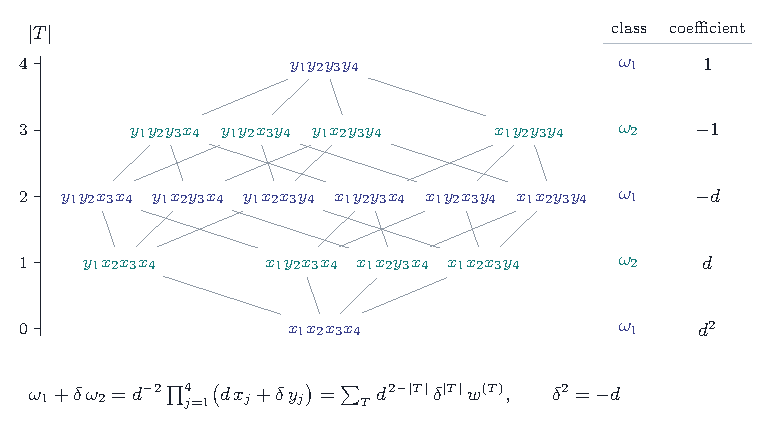
\includegraphics[width=0.78\textwidth]{fig_weilcube}
\caption{The $2^{2n}=16$ monomials $w^{(T)}$ of \Cref{not:wT} at $n=2$, as the
vertices of the $4$-cube, projected so that the height of $w^{(T)}$ is
$\lvert T\rvert$. An edge joins two monomials whose index sets differ in one
element, that is, two monomials related by a single substitution
$x_{j}\mapsto y_{j}$. The two colours are the bipartition by the parity of
$\lvert T\rvert$: the eight even vertices carry $\omega_{1}$ and the eight odd
ones carry $\omega_{2}$. The coefficient of $w^{(T)}$ depends only on
$\lvert T\rvert$ and is given by \eqref{eq:n2omega1} and
\eqref{eq:n2omega2}.}
\label{fig:weilcoeff}
\end{figure}

\subsection{Disjoint supports}

\Cref{prop:notpoly} is deduced from the character computation of
\Cref{sec:characters}. In the model the Weil line can be separated from the
powers of the polarisation without any representation theory: the Weil
classes and the powers of $\eta$ are supported on disjoint sets of monomials.

\begin{proposition}[Disjoint supports]\label{prop:disjoint}
In the model of \Cref{thm:model}, every monomial occurring in $\omega_{1}$ or
in $\omega_{2}$ contains exactly one of $x_{j},y_{j}$ for every
$j\in\{1,\dots,2n\}$, and every monomial occurring in $\eta^{k}$ contains
either both or neither, for every $j$ and every $k\ge0$. Consequently
\[
  \HW(A)\cap\QQ\,\eta^{n}=0 ,
\]
and more generally $\HW(A)$ meets the span of the monomials occurring in
powers of $\eta$ in zero.
\end{proposition}

\begin{proof}
The first assertion holds by \eqref{eq:omegagens} and \Cref{not:wT}. For the
second, $\eta$ is the combination \eqref{eq:etabasis} of the $2n$ two-forms
$x_{j}\wedge y_{j}$, which pairwise commute and square to zero, so
\[
  \eta^{k}=k!\sum_{\substack{S\subseteq\{1,\dots,2n\}\\|S|=k}}
    \Bigl(\prod_{j\in S}\epsilon_{j}\Bigr)\,
    \bigwedge_{j\in S}\bigl(x_{j}\wedge y_{j}\bigr),
\]
and the monomial indexed by $S$ contains both $x_{j}$ and $y_{j}$ for $j\in S$
and neither for $j\notin S$. A monomial cannot satisfy both patterns for a
given $j$, and since $2n\ge1$ there is at least one index at which to test,
so the two families of monomials are disjoint. Since
$\omega_{1},\omega_{2}$ span $\HW(A)$ by \Cref{thm:explicitgens}(ii), a nonzero
element of $\HW(A)$ has a nonzero coefficient on some $w^{(T)}$. As the
monomials form a basis of $\bigwedge^{2n}V$ and $w^{(T)}$ occurs in no power
of $\eta$, such an element does not lie in the span of the monomials
occurring in powers of $\eta$, and in particular not in $\QQ\,\eta^{n}$.
\end{proof}

\begin{remark}\label{rem:twoproofs}
The two proofs that the Weil line misses the powers of the polarisation
differ in scope. \Cref{prop:disjoint} concerns one model and one basis, and it
is short because the basis makes the $K$-action block diagonal. The
character proof is basis free, applies to every abelian variety of Weil type,
and identifies the obstruction as a difference of characters. The first can
be checked by hand; the second is the argument that \Cref{thm:character}
extends.
\end{remark}

\subsection{The Hodge ring of a general member}

It remains to count the Hodge classes, which measures how much of the Hodge
conjecture for $A$ is at stake. The Hodge classes of an abelian variety are
the invariants of its Hodge group, the special Mumford--Tate group
$\Hg(A)\subseteq\SL(V)$ \cite{Del82}:
$\Hdg^{k}(A)=H^{2k}(A,\QQ)^{\Hg(A)}$.

\begin{lemma}[The Hodge group]%
\label{lem:HgSU}
Let $(A,\iota,\eta)$ be of $(K,-1,n)$-Weil type and let $H$ be the
$K$-hermitian form of \Cref{lem:hermform}. Then
\[
  \Hg(A)\subseteq\SU(V,H) .
\]
\end{lemma}

\begin{proof}
The group $\Hg(A)$ is a $\QQ$-algebraic subgroup of $\SL(V)$ which fixes
every Hodge class in every tensor construction on $V$. It fixes
$\eta\in\bigwedge^{2}V$, hence preserves $Q$; and it commutes with $\iota(K)$,
because each $\iota(\tau)$ is a Hodge class in $V\otimes V^{\vee}$. A
$\QQ$-linear automorphism of $V$ commuting with the $K$-action and preserving
$Q$ preserves $H$, by the formula \eqref{eq:QfromH} expressing $H$ through $Q$
and the $K$-action. Hence $\Hg(A)\subseteq\mathrm{U}(V,H)$. Now
$\HW(A)$ consists of Hodge classes by \Cref{prop:weilline}(ii), so $\Hg(A)$
fixes $\HW(A)\otimes\CC$ pointwise, and in particular it fixes the line
$\bigwedge^{2n}V_{+}$ pointwise. An element $g\in\mathrm{U}(V,H)$ acts on
$\bigwedge^{2n}V_{+}$ by $\det_{K}(g)$,
so every $g\in\Hg(A)$ has $\det_{K}(g)=1$, which is the definition of
$\SU(V,H)$.
\end{proof}

For a very general member of the Weil family, that is, for every member whose
point in the period domain $\cD_{n,n}$ of \Cref{prop:weildomain} lies outside
a certain countable union of proper closed analytic subsets, the containment
of \Cref{lem:HgSU} is an equality; this is Weil's theorem \cite{Weil77}, in the
form given by Moonen and Zarhin \cite{MZ99}. The restriction to very general
members cannot be replaced by a Zariski open condition, since the locus where
the endomorphism algebra jumps is a countable union of such subsets, by
\Cref{thm:cdk}, and is dense in the classical topology. For such a member the
Hodge classes can be counted in every degree.

\begin{theorem}[The Hodge ring of a general member]\label{thm:hdgcount}
Let $(A,\iota,\eta)$ be of $(K,-1,n)$-Weil type with
$\Hg(A)=\SU(V,H)$. Then for every $k$ with $0\le k\le 2n$,
\[
  \dim_{\QQ}\Hdg^{k}(A)=
  \begin{cases}
    3, & k=n,\\[2pt]
    1, & k\ne n,
  \end{cases}
  \qquad\text{and}\qquad
  \Hdg^{n}(A)=\QQ\,\eta^{n}\oplus\HW(A).
\]
\end{theorem}

\begin{proof}
Complexify. The group $\SU(V,H)\otimes\CC$ is $\SL(V_{+})\cong\SL_{2n}(\CC)$,
acting on $V_{+}$ tautologically and on $V_{-}$ through the isomorphism
$V_{-}\cong V_{+}^{\vee}$ induced by $H$. By \Cref{prop:grading},
\[
  H^{2k}(A,\CC)=\bigoplus_{r+s=2k}
    \textstyle\bigwedge^{r}V_{+}\otimes\bigwedge^{s}V_{+}^{\vee},
\]
so it suffices to find the invariants in each summand. An invariant is a
weight-zero vector annihilated by every raising operator. Fix a basis of
$V_{+}$, take the diagonal torus of $\SL(V_{+})$ as maximal torus, and for
$T,U\subseteq\{1,\dots,2n\}$ let $v_{T}\in\bigwedge^{|T|}V_{+}$ and
$v_{U}^{\vee}\in\bigwedge^{|U|}V_{+}^{\vee}$ be the corresponding monomials in
the basis and its dual. In the weight lattice of $\SL_{2n}$ the weight of
$v_{T}\otimes v_{U}^{\vee}$ is
$\mathbf{1}_{T}-\mathbf{1}_{U}$ modulo $(1,1,\dots,1)$; since the entries of
$\mathbf{1}_{T}-\mathbf{1}_{U}$ lie in $\{-1,0,1\}$, the only multiples of
$(1,\dots,1)$ it can equal are $0$ and $\pm(1,\dots,1)$, giving
\[
  T=U \quad(\text{so } r=s),
  \qquad
  (T,U)=\bigl(\{1,\dots,2n\},\emptyset\bigr),
  \qquad
  (T,U)=\bigl(\emptyset,\{1,\dots,2n\}\bigr).
\]
The last two occur only for $(r,s)=(2n,0)$ and $(0,2n)$, each with a
one-dimensional weight-zero space consisting of the invariant lines
$\bigwedge^{2n}V_{+}$ and $\bigwedge^{2n}V_{-}$, which are $\SL$-invariant
because $\SL$ has trivial determinant. For $r=s$ the weight-zero space has
dimension $\binom{2n}{r}$ and its invariant subspace is the line spanned by the
image of the identity under
$\End(\bigwedge^{r}V_{+})\cong\bigwedge^{r}V_{+}\otimes\bigwedge^{r}V_{+}^{\vee}$,
which is one dimensional because $\bigwedge^{r}V_{+}$ is an irreducible
$\SL_{2n}$-module and Schur's lemma applies.

Collecting the contributions: for $k\ne n$ the only one is $(r,s)=(k,k)$, of
dimension one and spanned by $\eta^{k}$, which is a nonzero invariant lying in
that summand by \Cref{lem:NSchar}. For $k=n$ there are three contributions,
$(n,n)$, $(2n,0)$ and $(0,2n)$, of total dimension three; the first is spanned
by $\eta^{n}$ and the last two span $\HW(A)\otimes\CC$ by \Cref{lem:weilchar}.
Taking invariants commutes with extension of scalars from $\QQ$ to $\CC$, so
the dimensions over $\QQ$ are the same.
\end{proof}

\Cref{fig:hodgespike} displays these dimensions for $n=2,3,4$.

\begin{corollary}[Reduction to one class]\label{cor:whatisleft}
Let $(A,\iota,\eta)$ be as in \Cref{thm:hdgcount}. The Hodge conjecture holds
for $A$ in every degree if and only if the single class $\omega_{1}$ of
\eqref{eq:omegagens} is algebraic.
\end{corollary}

\begin{proof}
For $k\ne n$ the Hodge classes are the multiples of $\eta^{k}$, which are
algebraic, being powers of a divisor class. For $k=n$ they are spanned by
$\eta^{n}$, $\omega_{1}$ and $\omega_{2}$ by \Cref{thm:hdgcount}. Finally,
$\omega_{2}$ is algebraic as soon as $\omega_{1}$ is. By
\Cref{thm:explicitgens}(iv) the plane $\HW(A)$ is a free $K$-module of rank one
generated by $\omega_{1}$. For $\tau\in\Kx$ some positive integer multiple
$m\,\iota(\tau)$ lies in $\End(A)$, and on $H^{2n}(A,\QQ)$ the operator
$\iota(\tau)^{*}$ is $m^{-2n}$ times the pullback by $m\,\iota(\tau)$, so it
carries algebraic classes to algebraic classes. Any $\tau$ with
$\tau^{2n}\notin\QQ$, which exists by the argument of \Cref{lem:charsdiffer},
moves $\omega_{1}$ to a class with a nonzero $\omega_{2}$ component, and so
$\omega_{2}$ is a rational combination of the algebraic classes $\omega_{1}$
and $\iota(\tau)^{*}\omega_{1}$.
\end{proof}

\begin{remark}\label{rem:onlyoneclass}
\Cref{cor:whatisleft} explains why the Weil line is the standard test case. On a
general abelian variety of Weil type the Hodge conjecture concerns one
explicitly written class with $2^{2n-1}$ integer coefficients, and no space of
classes of unknown structure. The obstruction theorems of this paper
constrain the ways in which that class can be produced, and
\Cref{sec:basepoints} exhibits in every Weil family a member on which the
whole Weil line consists of polynomials in divisor classes.
\end{remark}

\begin{figure}[htbp]
\centering
  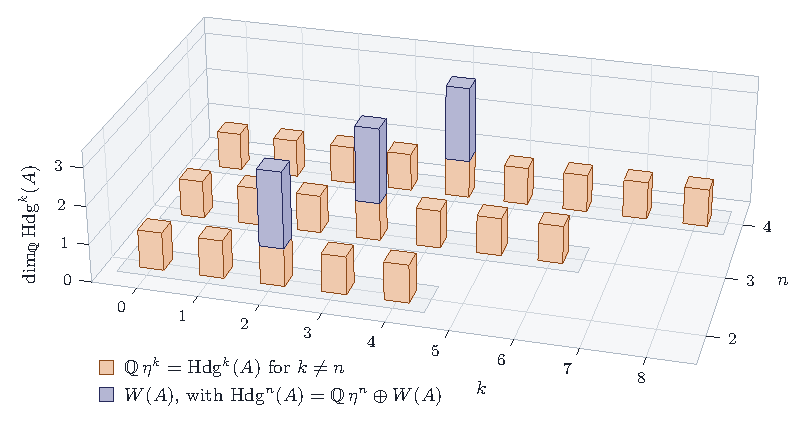
\includegraphics[width=0.9\textwidth]{fig_hodgespike}
\caption{The dimensions of $\Hdg^{k}(A)$ for a general abelian variety of
$(K,-1,n)$-Weil type, $0\le k\le 2n$, at $n=2,3,4$, as computed in
\Cref{thm:hdgcount}. Every degree carries the line $\QQ\,\eta^{k}$; the middle
degree $k=n$ carries in addition the two dimensions of the Weil line
$\HW(A)$, and nothing else occurs. The profile is the same for every $n$.}
\label{fig:hodgespike}
\end{figure}

\section{The character grading and the position of the Weil line}
\label{sec:characters}

This section proves the character obstruction, \Cref{thm:character}, which
is used in the proof of \Cref{prop:notpoly}. The group $\Kx$
acts on $H^{2n}(A,\QQ)$ through the endomorphisms $\iota(\tau)$. This action
grades the cohomology, and the Weil line and the power $\eta^{n}$ of the
polarisation lie in different graded pieces; once the grading is written
down, the obstruction follows in a few lines. The one point that needs care
is the character through which $\Kx$ acts on the Weil line. It is
$\tau\mapsto\tau^{2n}$, together with its conjugate, and not a power of the
norm, even though the Weil line is a $K$-line and multiplication by $\tau$ on
a $K$-line has determinant $\Nm(\tau)$ (\Cref{rem:failuremode}).

\subsection{The grading}

Throughout this section $(A,\iota,\eta)$ is of $(K,-1,n)$-Weil type,
$V=H^{1}(A,\QQ)$, and $V_{\CC}=V_{+}\oplus V_{-}$ is the splitting of
\Cref{not:eigen}.

\begin{proposition}[Character grading]\label{prop:grading}
For every $k\ge0$,
\begin{equation}\label{eq:grading}
  H^{k}(A,\CC)\;=\;\bigoplus_{r+s=k}
    \Bigl(\textstyle\bigwedge^{r}V_{+}\otimes\bigwedge^{s}V_{-}\Bigr),
\end{equation}
and $\iota(\tau)^{*}$ acts on the summand indexed by $(r,s)$ by the scalar
$\tau^{r}\bbar{\tau}^{\,s}$. The summands are the isotypic components for the
action of $\Kx$, and the characters $\tau\mapsto\tau^{r}\bbar{\tau}^{\,s}$ for
distinct pairs $(r,s)$ with $r+s=k$ are pairwise distinct.
\end{proposition}

\begin{proof}
By \eqref{eq:wedge}, $H^{k}(A,\CC)=\bigwedge^{k}V_{\CC}$, and the exterior
power of a direct sum decomposes as
$\bigwedge^{k}(V_{+}\oplus V_{-})=\bigoplus_{r+s=k}\bigwedge^{r}V_{+}\otimes\bigwedge^{s}V_{-}$,
which is \eqref{eq:grading}. By \Cref{not:eigen}, $\iota(\tau)^{*}$ acts on
$V_{+}$ by $\tau$ and on $V_{-}$ by $\bbar{\tau}$. Since it is an algebra
homomorphism for the wedge product, it acts on
$\bigwedge^{r}V_{+}\otimes\bigwedge^{s}V_{-}$ by $\tau^{r}\bbar{\tau}^{\,s}$.

For the last statement, suppose that
$\tau^{r}\bbar{\tau}^{\,s}=\tau^{r'}\bbar{\tau}^{\,s'}$ for all $\tau\in\Kx$,
where $r+s=r'+s'=k$. Then $s-s'=r'-r$, and dividing gives
$(\tau/\bbar{\tau})^{r-r'}=1$ for every $\tau\in\Kx$. If $r\ne r'$, the image
of the map $c(\tau)=\tau/\bbar{\tau}$ therefore lies in the group of
$(r-r')$-th roots of unity of $K$, which is finite: the group of all roots of
unity of the imaginary quadratic field $K$ has order $2$, $4$ or $6$. But $c$
has infinite image. Two elements have the same image exactly when their ratio
lies in $\QQ^{\times}$, and the elements $m+\sqrt{-d}$ with $m\in\ZZ$ are
pairwise non-proportional over $\QQ$. Hence $r=r'$, and so $s=s'$. Since the
characters of the summands are pairwise distinct, the summands are the
isotypic components.

The distinctness is that of characters of the torus
$\Res_{K/\QQ}\mathbb{G}_{m}$, not of their values at a given $\tau$: the
values at $\tau$ for $(r,s)$ and $(r',s')$ agree if and only if
$\tau/\bbar{\tau}$ is a root of unity of order dividing $r-r'$, and this can
happen (\Cref{rem:witness}).
\end{proof}

\begin{lemma}[The polarisation sits in the middle]\label{lem:NSchar}
Let $(A,\iota,\eta)$ be of $(K,-1,n)$-Weil type. Then
\[
  \iota(\tau)^{*}\eta=\Nm_{K/\QQ}(\tau)\,\eta\qquad\text{for all }\tau\in\Kx,
\]
so $\eta$ lies in the summand $(r,s)=(1,1)$ of \eqref{eq:grading} and
$\eta^{n}$ lies in the summand $(r,s)=(n,n)$, on which $\Kx$ acts by $\Nm^{n}$.
\end{lemma}

\begin{proof}
Let $E$ be the alternating form on $H_{1}(A,\QQ)$ attached to $\eta$. By
condition (iii) of \Cref{def:weiltype}, the Rosati involution $\dagger$ of
$\eta$ satisfies $\iota(\tau)^{\dagger}=\iota(\bbar{\tau})$, so by the
defining property of the Rosati involution
\[
  E\bigl(\iota(\tau)x,\,y\bigr)=E\bigl(x,\,\iota(\tau)^{\dagger}y\bigr)
  =E\bigl(x,\,\iota(\bbar{\tau})y\bigr)
  \qquad\text{for all }x,y .
\]
Therefore
\begin{align*}
  \bigl(\iota(\tau)^{*}E\bigr)(x,y)
  &=E\bigl(\iota(\tau)x,\iota(\tau)y\bigr)
   =E\bigl(x,\iota(\bbar{\tau})\iota(\tau)y\bigr)\\
  &=E\bigl(x,\iota(\Nm(\tau))y\bigr)=\Nm(\tau)\,E(x,y),
\end{align*}
using $\bbar{\tau}\tau=\Nm(\tau)\in\QQ$ and the $\QQ$-linearity of $\iota$.
Under the identification of $H^{2}(A,\QQ)=\bigwedge^{2}H^{1}(A,\QQ)$ with the
alternating forms on $H_{1}(A,\QQ)$, which is compatible with pullback, $\eta$
corresponds to $E$, so this is the displayed identity. Since
$\Nm(\tau)=\tau\bbar{\tau}$, \Cref{prop:grading} identifies the isotypic
component of $\Nm$ in $H^{2}(A,\CC)$ with the summand $(r,s)=(1,1)$, and
$\eta$ lies in it. Because $\iota(\tau)^{*}$ is a ring homomorphism,
$\iota(\tau)^{*}\eta^{n}=\Nm(\tau)^{n}\eta^{n}$, and in the same way this
places $\eta^{n}$ in the summand $(n,n)$.
\end{proof}

\begin{lemma}[The Weil line sits at the ends]\label{lem:weilchar}
Let $(A,\iota,\eta)$ be of $(K,-1,n)$-Weil type. Then
\[
  \HW(A)\otimes_{\QQ}\CC
  =\Bigl(\textstyle\bigwedge^{2n}V_{+}\Bigr)\oplus
   \Bigl(\textstyle\bigwedge^{2n}V_{-}\Bigr),
\]
the summands $(r,s)=(2n,0)$ and $(0,2n)$ of \eqref{eq:grading} in degree $2n$,
on which $\Kx$ acts by $\tau\mapsto\tau^{2n}$ and $\tau\mapsto\bbar{\tau}^{\,2n}$.
\end{lemma}

\begin{proof}
This is \Cref{def:weilline} together with \Cref{prop:weilline}(i), which says
that $\HW(A)$ is the $\QQ$-structure on that pair of lines; the characters are
read off from \Cref{prop:grading} with $(r,s)=(2n,0)$ and $(0,2n)$.
\end{proof}

\begin{lemma}[The two characters differ]\label{lem:charsdiffer}
For every $n\ge1$ the characters $\tau\mapsto\tau^{2n}$ and
$\tau\mapsto\Nm_{K/\QQ}(\tau)^{n}=(\tau\bbar{\tau})^{n}$ of $\Kx$ are distinct,
as are $\tau\mapsto\bbar{\tau}^{\,2n}$ and $\Nm^{n}$.
\end{lemma}

\begin{proof}
This is the case $(r,s)=(2n,0)$, $(r',s')=(n,n)$ of the last assertion of
\Cref{prop:grading}; we write the argument out in this case. For $\tau\ne0$
the identity $\tau^{2n}=(\tau\bbar{\tau})^{n}$ is equivalent to
$(\tau/\bbar{\tau})^{n}=1$, so the two characters agree if and only if
$(\tau/\bbar{\tau})^{n}=1$ for every $\tau\in\Kx$.

Consider the map $c\colon\Kx\to\Kx$, $c(\tau)=\tau/\bbar{\tau}$. Two elements
have the same image if and only if their ratio is fixed by conjugation, that
is, lies in $\QQ^{\times}$. The elements $m+\sqrt{-d}$ with $m\in\ZZ$ are
pairwise non-proportional over $\QQ$, so $c$ takes infinitely many values.

On the other hand, $\{\zeta\in K:\zeta^{n}=1\}$ is contained in the group
$\mu(K)$ of roots of unity of $K$, and for an imaginary quadratic field
$\mu(K)$ is finite: it has order $4$ for $d=1$, order $6$ for $d=3$, and order
$2$ otherwise. Since the image of $c$ is infinite, it is not contained in this
finite set, so some $\tau\in\Kx$ has $(\tau/\bbar{\tau})^{n}\ne1$, and the
characters differ. The second pair is obtained from the first by conjugation.
\end{proof}

\begin{remark}[Explicit witnesses]\label{rem:witness}
The proof does not exhibit a $\tau$ at which the two characters differ, and
the natural candidate $\tau=1+\sqrt{-d}$ is not always one. For $d=1$ its
ratio $\tau/\bbar{\tau}$ is $\sqrt{-1}$, a primitive fourth root of unity, so
the two characters agree at this $\tau$ whenever $4\mid n$; for $d=3$ the
ratio is $(-1+\sqrt{-3})/2$, a primitive cube root of unity, and they agree
whenever $3\mid n$. The candidate $\tau=3+\sqrt{-d}$ fails as well, at $d=3$
with $6\mid n$, where the ratio is $(1+\sqrt{-3})/2$, a primitive sixth root of
unity. In each case the characters agree at $\tau$ exactly when the order of
the ratio divides $n$. The element $\tau=2+\sqrt{-d}$ is a witness for every $d$
and every $n$. Its ratio is $\bigl(4-d+4\sqrt{-d}\bigr)/(4+d)$, which is not
$\pm1$, and for $d\notin\{1,3\}$ these are the only roots of unity in $K$;
for $d=1$ and $d=3$ the ratios $(3+4\sqrt{-1})/5$ and $(1+4\sqrt{-3})/7$ are
not roots of unity either, since their traces $6/5$ and $2/7$ are not
integers. The same holds for $4+\sqrt{-d}$ and $3+2\sqrt{-d}$. The finiteness
argument in the proof covers all fields at once and needs no witness. \Cref{fig:witness} shows the powers of these ratios for $d=1$ and $d=3$.
\end{remark}

\begin{figure}[htbp]
\centering
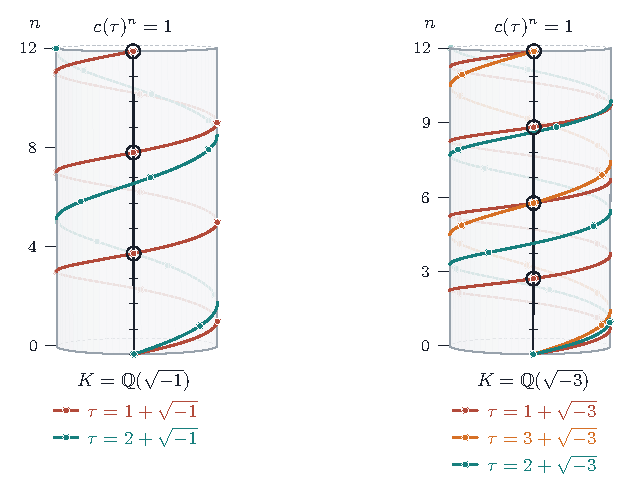
\includegraphics[width=0.78\textwidth]{fig_witness}
\caption{\Cref{rem:witness}. The values $c(\tau)^{n}=(\tau/\bbar\tau)^{n}$,
$0\le n\le12$, on the unit circle, stacked over $n$ as a helix; the
characters $\tau^{2n}$ and $\Nm^{n}$ agree at $\tau$ exactly where the helix
meets the vertical line $c^{n}=1$ (circled). Left, $K=\QQ(\sqrt{-1})$: the
candidate $1+\sqrt{-1}$ returns every fourth step, and $2+\sqrt{-1}$ never.
Right, $K=\QQ(\sqrt{-3})$: $1+\sqrt{-3}$ returns every third step,
$3+\sqrt{-3}$ every sixth, and $2+\sqrt{-3}$ never.}
\label{fig:witness}
\end{figure}

\subsection{The obstruction}

\begin{theorem}[Character obstruction]\label{thm:character}
Let $(A,\iota,\eta)$ be of $(K,-1,n)$-Weil type and write
$H^{1}(A,\QQ)\otimes\CC=V_{+}\oplus V_{-}$ for the decomposition into
eigenspaces of $\iota(\sqrt{-d})$. Then
\[
  H^{2n}(A,\QQ)\otimes\CC
  =\bigoplus_{r+s=2n}\textstyle\bigwedge^{r}V_{+}\otimes\bigwedge^{s}V_{-},
\]
with $\iota(\tau)$ acting on the $(r,s)$ summand by
$\tau^{r}\bbar{\tau}^{\,s}$.
The Weil line $\HW(A)$ spans the two extreme summands $(r,s)=(2n,0)$ and
$(0,2n)$, on which $\Kx$ acts by $\tau^{2n}$ and $\bbar{\tau}^{2n}$, while
$\eta^{n}$ lies in the middle summand $(r,s)=(n,n)$, on which $\Kx$ acts by
the norm character $\Nm_{K/\QQ}(\tau)^{n}$. In particular, for every $n\ge1$,
\[
  \HW(A)\cap H^{2n}(A,\QQ)^{\Nm^{n}}=0,
\]
so a class that is a $\Kx$-eigenclass for $\Nm^{n}$ has zero component along
the Weil line.
\end{theorem}

The theorem shows that the obstruction is structural. A construction that is
equivariant for the $K$-action returns an eigenclass, so it must choose a
character in advance, and the norm character is the one that the
polarisation already occupies. The Weil line sits at the two ends of the
$\Kx$-grading, as far from the middle as the grading allows;
\Cref{fig:charactergrid} draws the grading and marks the two positions.

\begin{proof}[Proof of \Cref{thm:character}]
The grading \eqref{eq:grading} and the action on its summands are given by
\Cref{prop:grading}, the position of $\HW(A)$ by \Cref{lem:weilchar}, and
that of $\eta^{n}$ by \Cref{lem:NSchar}. For the last assertion, write
$H^{2n}(A,\QQ)^{\Nm^{n}}$ for the space of classes $x$ with
$\iota(\tau)^{*}x=\Nm(\tau)^{n}x$ for all $\tau\in\Kx$. After extension of
scalars to $\CC$ this is the isotypic component of the character $\Nm^{n}$,
which by \Cref{prop:grading} is the single summand $(r,s)=(n,n)$. By
\Cref{lem:charsdiffer} the characters $\tau^{2n}$ and $\bbar{\tau}^{\,2n}$
differ from $\Nm^{n}$, so by \Cref{lem:weilchar} the space
$\HW(A)\otimes\CC$ meets the summand $(n,n)$ in zero. Intersecting with
$H^{2n}(A,\QQ)$ gives $\HW(A)\cap H^{2n}(A,\QQ)^{\Nm^{n}}=0$.
\end{proof}

\begin{corollary}[Equivariant classes]%
\label{cor:equivariant}
Let $x\in H^{2n}(A,\QQ)$ satisfy $\iota(\tau)^{*}x=\Nm(\tau)^{n}x$ for all
$\tau\in\Kx$. Then the component of $x$ along $\HW(A)$, with respect to any
$\Kx$-stable complement of $\HW(A)$, is zero. In particular, $x$ is a Weil
class only if $x=0$.
\end{corollary}

\begin{proof}
Let $C$ be a $\Kx$-stable complement of $\HW(A)$ in $H^{2n}(A,\QQ)$ and let
$p$ be the projection onto $\HW(A)$ along $C$. Since both summands are
$\Kx$-stable, $p$ commutes with every $\iota(\tau)^{*}$, so
$\iota(\tau)^{*}p(x)=\Nm(\tau)^{n}p(x)$ for all $\tau\in\Kx$. Hence $p(x)$
lies in $\HW(A)\cap H^{2n}(A,\QQ)^{\Nm^{n}}$, which is zero by
\Cref{thm:character}. If $x$ is a Weil class, then $x=p(x)=0$.
\end{proof}

\Cref{cor:equivariant} is the form of the obstruction that applies to
constructions. A construction that is natural in the $K$-action produces an
eigenclass, whose character is determined by how the input transforms. The
only character available to a rational eigenclass in $H^{2n}(A,\QQ)$ is
$\Nm^{n}$ (\Cref{rem:rightcharacter}). By \Cref{lem:NSchar} this character is
already occupied by the polarisation, and by \Cref{lem:charsdiffer} it is not
a character of the Weil line.

\begin{remark}[Rational eigenclasses]\label{rem:rightcharacter}
To land on the Weil line, a construction must produce classes on which $\Kx$
acts through $\tau\mapsto\tau^{2n}$ or $\tau\mapsto\bbar{\tau}^{\,2n}$, and
neither character is $\QQ$-valued. This rules out rational eigenclasses.
Indeed, let $0\ne x\in H^{k}(A,\QQ)$ satisfy $\iota(\tau)^{*}x=\chi(\tau)\,x$
for all $\tau\in\Kx$. Then $\chi(\tau)\in\QQ$, because $\iota(\tau)^{*}$
preserves $H^{k}(A,\QQ)$. By \Cref{prop:grading}, $x$ lies in a single summand
$(r,s)$ and $\chi(\tau)=\tau^{r}\bbar{\tau}^{\,s}$. Since $\chi$ is
$\QQ$-valued, it equals its conjugate $\tau\mapsto\tau^{s}\bbar{\tau}^{\,r}$,
and the distinctness of the characters in \Cref{prop:grading} gives $r=s$. So
every rational $\Kx$-eigenclass in $H^{2n}(A,\QQ)$ is an eigenclass for
$\Nm^{n}$, and \Cref{cor:equivariant} applies to it. A construction that
reaches the Weil line must therefore produce a class that is not a
$\Kx$-eigenclass. A nonzero element of $\HW(A)$ has nonzero components in both
summands $(2n,0)$ and $(0,2n)$, since complex conjugation interchanges them,
and its $\Kx$-orbit spans the $\QQ$-plane $\HW(A)$. No rational eigenvalue
condition isolates the Weil line: such conditions cut out only the diagonal
summands $(r,r)$, and the Weil line lies at the two ends of the grading.
\end{remark}

\begin{remark}[Determinant and character]\label{rem:failuremode}
A natural chain of statements leads to the opposite conclusion, that $\Kx$
acts on the Weil line through a power of the norm. The Weil line is
$\bigwedge^{2n}_{K}V$, a free $K$-module of rank one; such a module is
two-dimensional over $\QQ$; and multiplication by $\tau$ on it is a
$\QQ$-linear map of determinant $\Nm(\tau)$. Each statement is true, but the
last concerns the $K$-module structure and not the action of $\iota(\tau)$.
By \Cref{lem:weilchar}, $\iota(\tau)$ acts on the Weil line as multiplication
by $\tau^{2n}$, with determinant $\Nm(\tau)^{2n}$, and a space on which $\Kx$
acts through multiplication by $\tau^{2n}$ is not one on which it acts by the
scalar $\Nm(\tau)^{n}$. The first is a $K$-line and the second a
$\QQ$-eigenspace, and they would agree only if $\tau^{n}=\bbar{\tau}^{\,n}$
for all $\tau\in\Kx$, which \Cref{lem:charsdiffer} excludes.
\Cref{fig:charactergrid} draws the distinction.
\end{remark}

\begin{figure}[htbp]
\centering
  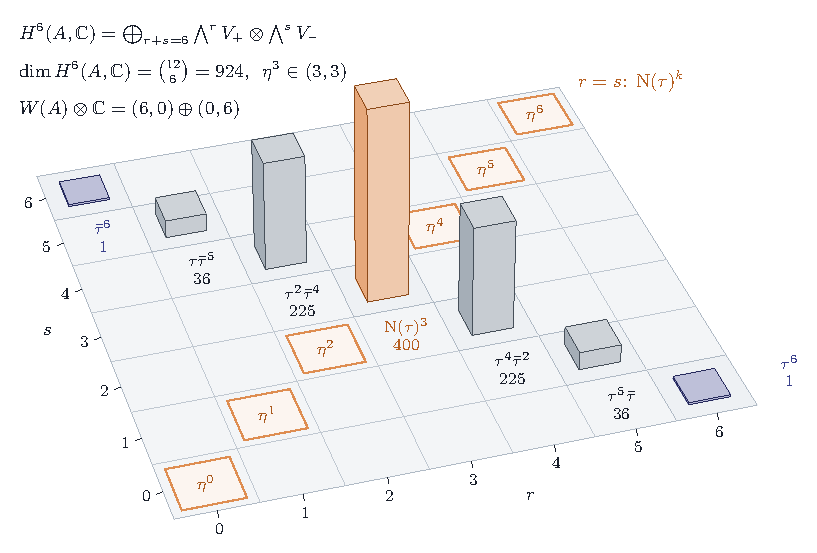
\includegraphics[width=\textwidth]{fig_charactergrid}
\caption{The $\Kx$-grading at $n=3$ on the grid of pairs $(r,s)$,
$0\le r,s\le 6$. The summands $\bigwedge^{r}V_{+}\otimes\bigwedge^{s}V_{-}$ of
$H^{6}(A,\CC)$ lie on the antidiagonal $r+s=6$ and are drawn at their
dimensions $\binom{6}{r}\binom{6}{s}$, which sum to $\binom{12}{6}=924$; on
the summand $(r,s)$ the group $\Kx$ acts by $\tau^{r}\bbar{\tau}^{\,s}$. The
two end cells $(6,0)$ and $(0,6)$, with characters $\tau^{6}$ and
$\bbar{\tau}^{\,6}$, span the Weil line; the middle cell $(3,3)$, with
character $\Nm(\tau)^{3}$, contains $\eta^{3}$. The outlined cells on the
diagonal $r=s$ are the summands on which $\Kx$ acts through a power of the
norm, and they carry the powers $\eta^{k}$. That the end cells and the middle
cell differ is the content of \Cref{thm:character}.}
\label{fig:charactergrid}
\end{figure}

\section{The cohomological Fourier--Mukai transform}\label{sec:fm}

With the character obstruction proved, we turn to the divisor obstruction of
\Cref{thm:divisor}. Its one nontrivial ingredient is a computation: the
cohomological Fourier--Mukai transform sends each power of the polarisation
class to a rational multiple of a power of the polarisation class on the
other side. We prove this in closed form. The computation takes place in a
cohomology ring which, together with the classes involved, depends up to
isomorphism only on the dimension, so one calculation covers every
principally polarised abelian variety at once. Since the Todd class of an
abelian variety is trivial, the passage from sheaves to cohomology is a
formal step.

\subsection{Grothendieck--Riemann--Roch on an abelian variety}

\begin{proposition}\label{prop:grr}
Let $A$ be an abelian variety of dimension $g$ and $\cG$ an object of
$D^{b}(\Av)$. Then
\[
  \ch\bigl(\Phi_{\cP}(\cG)\bigr)=\Phi_{\cP}\bigl(\ch(\cG)\bigr),
\]
where the transform on the right is the cohomological one,
$\Phi_{\cP}(x)=p_{*}\bigl(q^{*}x\cdot\ch(\cP)\bigr)$.
\end{proposition}

\begin{proof}
Grothendieck--Riemann--Roch for the projection
$p\colon A\times\Av\to A$, a proper morphism of smooth varieties, reads
\[
  \ch\bigl(Rp_{*}\cK\bigr)\cdot\td(T_{A})
  =p_{*}\bigl(\ch(\cK)\cdot\td(T_{A\times\Av})\bigr)
\]
for $\cK\in D^{b}(A\times\Av)$. The tangent bundle of an abelian variety is
trivial, so $\td(T_{A})=1$ and $\td(T_{A\times\Av})=1$. Take
$\cK=Lq^{*}\cG\otimes^{L}\cP$, so that $Rp_{*}\cK=\Phi_{\cP}(\cG)$; the
multiplicativity of the Chern character and $\ch(Lq^{*}\cG)=q^{*}\ch(\cG)$
give the statement.
\end{proof}

\subsection{The universal model}

\begin{notation}\label{not:model}
Let $A$ be a principally polarised abelian variety of dimension $g$ with
polarisation class $\theta$, and put $V=H^{1}(A,\QQ)$, a $\QQ$-vector space of
dimension $2g$ carrying the symplectic form attached to $\theta$. Choose a
symplectic basis $e_{1},\dots,e_{2g}$ of $V$ for this form, so that
\begin{equation}\label{eq:thetamodel}
  \theta=\sum_{j=1}^{g}e_{j}\wedge e_{g+j}.
\end{equation}
The principal polarisation identifies $\Av$ with $A$ and
$H^{1}(\Av,\QQ)$ with the dual $V^{\vee}$; let $f_{1},\dots,f_{2g}$ be the
basis dual to $e_{1},\dots,e_{2g}$, so that
\begin{equation}\label{eq:thetapmodel}
  \theta'=\sum_{j=1}^{g}f_{j}\wedge f_{g+j}.
\end{equation}
Then $H^{*}(A\times\Av,\QQ)=\bigwedge^{*}(V\oplus V^{\vee})$.
\end{notation}

\begin{lemma}[The Poincar\'e class]\label{lem:poincare}
In the model of \Cref{not:model},
\begin{equation}\label{eq:ell}
  \ell\coloneqq c_{1}(\cP)=\sum_{i=1}^{2g}e_{i}\wedge f_{i}
  \;\in\;V\otimes V^{\vee}\subset\textstyle\bigwedge^{2}(V\oplus V^{\vee}),
\end{equation}
the canonical element of $V\otimes V^{\vee}=\Hom(V,V)$ corresponding to the
identity, and $\ch(\cP)=e^{\ell}$.
\end{lemma}

\begin{proof}
The Poincar\'e bundle is normalised to be trivial on $A\times\{0\}$ and on
$\{0\}\times\Av$. The components of $c_{1}(\cP)$ in $\bigwedge^{2}V$ and in
$\bigwedge^{2}V^{\vee}$ are its restrictions to these two subvarieties, so
they vanish, and $c_{1}(\cP)$ lies in the middle summand $V\otimes V^{\vee}$
of
$\bigwedge^{2}(V\oplus V^{\vee})=\bigwedge^{2}V\oplus(V\otimes V^{\vee})\oplus\bigwedge^{2}V^{\vee}$.
The defining property of $\cP$ is that its restriction to $A\times\{\lambda\}$
is the line bundle $\lambda$; on cohomology this says that the induced map
$H^{1}(\Av,\QQ)\to H^{1}(A,\QQ)^{\vee}$ obtained by contracting $c_{1}(\cP)$ is
the canonical identification. Equivalently, the element of $\Hom(V,V)$
determined by $c_{1}(\cP)$ is the identity, which is \eqref{eq:ell}. Since
$\cP$ is a line bundle, $\ch(\cP)=e^{c_{1}(\cP)}$.
\end{proof}

\begin{remark}\label{rem:universal}
Every principally polarised abelian variety of dimension $g$ gives, up to
isomorphism, the same data in \Cref{not:model}: a symplectic space of
dimension $2g$ over $\QQ$, its dual, the symplectic form, and the canonical
element. The constants computed
below therefore depend only on $g$ and $k$, and not on $A$.
\end{remark}

\subsection{The closed form}

\begin{theorem}[Transform of the polarisation powers]\label{thm:fmtheta}
Let $A$ be a principally polarised abelian variety of dimension $g$. Then for
every $0\le k\le g$,
\begin{equation}\label{eq:fmtheta}
  \Phi_{\cP}\bigl(\theta'^{\,k}\bigr)
  \;=\;(-1)^{\,g(g+1)/2\,+\,k}\,\frac{k!}{(g-k)!}\;\theta^{\,g-k},
\end{equation}
and $\Phi_{\cP}(\theta'^{\,k})=0$ for $k>g$. In particular
$\Phi_{\cP}\bigl(\QQ[\theta']\bigr)=\QQ[\theta]$.
\end{theorem}

\begin{proof}
Work in the model of \Cref{not:model}. By definition
$\Phi_{\cP}(x)=p_{*}(q^{*}x\cdot e^{\ell})$, and $p_{*}$ extracts the
coefficient of the top exterior form $f_{1}\wedge\cdots\wedge f_{2g}$ in the
$V^{\vee}$ variables: it sends $y\wedge f_{1}\wedge\cdots\wedge f_{2g}$ to
$y$ for $y\in\bigwedge^{*}V$, and kills every class of lower degree in the
$V^{\vee}$ variables.

The classes $e_{i}\wedge f_{i}$ have even degree, so they commute, and they
have square zero. Hence for every $m$,
\begin{equation}\label{eq:ellpower}
  \frac{\ell^{m}}{m!}
  =\sum_{\substack{S\subseteq\{1,\dots,2g\}\\ |S|=m}}\ \prod_{i\in S}e_{i}\wedge f_{i},
\end{equation}
the product being taken in increasing order of $i$. Likewise, from
\eqref{eq:thetapmodel},
\begin{equation}\label{eq:thetappower}
  \frac{\theta'^{\,k}}{k!}
  =\sum_{\substack{T\subseteq\{1,\dots,g\}\\ |T|=k}}\ \prod_{j\in T}f_{j}\wedge f_{g+j},
  \qquad
  \frac{\theta^{\,g-k}}{(g-k)!}
  =\sum_{\substack{U\subseteq\{1,\dots,g\}\\ |U|=g-k}}\ \prod_{j\in U}e_{j}\wedge e_{g+j}.
\end{equation}

Fix $k$. In the product $\theta'^{\,k}\cdot e^{\ell}$, the terms that survive
$p_{*}$ are those of total degree $2g$ in the $f$ variables. A term of
\eqref{eq:thetappower} indexed by $T$ carries the $2k$ variables
$\{f_{j},f_{g+j}:j\in T\}$, and a term of \eqref{eq:ellpower} indexed by $S$
carries the $|S|$ variables $\{f_{i}:i\in S\}$. For the product to be nonzero
the two index sets must be disjoint, and for the total $f$-degree to be $2g$
we need
\[
  S=\{1,\dots,2g\}\setminus\bigl(T\cup(g+T)\bigr),
  \qquad |S|=2g-2k .
\]
So $S$ is determined by $T$, only the term $\ell^{2g-2k}/(2g-2k)!$ of
$e^{\ell}$ contributes, and the surviving terms are in bijection with the
$k$-subsets $T$ of $\{1,\dots,g\}$. Writing $U=\{1,\dots,g\}\setminus T$ we
have $S=U\cup(g+U)$, so the $V$-part of the term indexed by $T$ is
$\prod_{i\in U\cup(g+U)}e_{i}$, which up to sign is the term of
\eqref{eq:thetappower} indexed by $U$. The bijection $T\leftrightarrow U$ is
the one between the terms of $\theta'^{\,k}/k!$ and those of
$\theta^{\,g-k}/(g-k)!$.

It remains to compute the sign $\sigma$ with which each term contributes, and
to check that it is the same for all $T$. The sign is that of the
rearrangement of the ordered word
\[
  \Bigl(\prod_{j\in T}f_{j}f_{g+j}\Bigr)\cdot\Bigl(\prod_{i\in S}e_{i}f_{i}\Bigr)
\]
into the target word
$\bigl(\prod_{j\in U}e_{j}e_{g+j}\bigr)\cdot\bigl(f_{1}\cdots f_{2g}\bigr)$,
which uses the same generators. Relabelling the $g$ symplectic pairs by a
permutation $\pi$ of $\{1,\dots,g\}$ is an automorphism of the exterior
algebra. It
carries the word for $T$ to the word for $\pi(T)$, because the blocks
$f_{j}f_{g+j}$ and $e_{i}f_{i}$ have degree two and may be reordered freely,
and it carries the target word for $U$ to the target word for $\pi(U)$,
because reordering
$f_{\pi(1)}\cdots f_{\pi(g)}f_{g+\pi(1)}\cdots f_{g+\pi(g)}$ costs the
square of the sign of $\pi$. Since the permutations of $\{1,\dots,g\}$ act
transitively on the $k$-subsets, $\sigma=\sigma(g,k)$, and we evaluate it at
$T=\{1,\dots,k\}$. Put $r=g-k$. Moving the $2r$ variables $e_{i}$ of the
second factor to its front costs $(-1)^{r(2r-1)}=(-1)^{r}$, moving them
further past the $2k$ variables of the first factor costs nothing, and
arranging them as $\prod_{j\in U}e_{j}e_{g+j}$ costs $(-1)^{r(r-1)/2}$. The
$f$ variables are left in the order
$f_{1}f_{g+1}\cdots f_{k}f_{g+k}\,f_{k+1}\cdots f_{g}\,f_{g+k+1}\cdots f_{2g}$,
and bringing them to $f_{1}\cdots f_{2g}$ costs $(-1)^{k(k-1)/2+rk}$. As
$r+r(r-1)/2+k(k-1)/2+rk=g(g+1)/2-k$, this gives
\begin{equation}\label{eq:sign}
  \sigma(g,k)=(-1)^{\,g(g+1)/2\,+\,k}.
\end{equation}
Assembling, and accounting for the factorials in \eqref{eq:thetappower},
\[
  \Phi_{\cP}(\theta'^{\,k})
  =k!\cdot\sigma(g,k)\cdot\frac{\theta^{\,g-k}}{(g-k)!},
\]
which is \eqref{eq:fmtheta}. For $k>g$ we have $\theta'^{\,k}=0$, because
$\theta'^{\,k}$ lies in $\bigwedge^{2k}V^{\vee}$, which vanishes for
$2k>2g$. The last assertion follows because the constants in
\eqref{eq:fmtheta} are nonzero for every $0\le k\le g$.
\end{proof}

\begin{remark}[The sign]\label{rem:signcheck}
The sign \eqref{eq:sign} depends only on $g$ and $k$, by the transitivity
argument in the proof, and the count at $T=\{1,\dots,k\}$ fixes it. For even $g=2n$, the case of Weil type,
$g(g+1)/2=n(2n+1)$ has the parity of $n$, and \eqref{eq:sign} reads
$\sigma(2n,k)=(-1)^{n+k}$.
\end{remark}

\begin{corollary}[Stability of the polarisation subring]\label{cor:stability}
Let $A$ be a principally polarised abelian variety and let
$x\in H^{*}(\Av,\QQ)$ lie in the subring $\QQ[\theta']$ generated by $\theta'$.
Then $\Phi_{\cP}(x)\in\QQ[\theta]$.
\end{corollary}

\begin{proof}
The ring $\QQ[\theta']$ is spanned over $\QQ$ by the powers
$\theta'^{\,k}$, \Cref{thm:fmtheta} sends each of them to a rational
multiple of a power of $\theta$, and $\Phi_{\cP}$ is linear.
\end{proof}

\begin{remark}[Non-principal polarisations]\label{rem:nonprincipal}
If $\theta$ is a polarisation of degree $D^{2}$ rather than a principal
one, the isogeny $\phi_{\theta}\colon A\to\Av$ has degree $D^{2}$,
and $\phi_{\theta}^{*}\theta'=D\theta$ for a suitable normalisation of
$\theta'$. The argument of \Cref{thm:fmtheta} goes through with $\theta$
replaced by $D^{-1}\phi_{\theta}^{*}\theta'$, and the constants change
by powers of $D$, all of which are nonzero rationals. The statements below
concern only membership in $\QQ[\theta]$, not the values of the constants, so
we state them for principal polarisations and use them in general.
\end{remark}

\section{The divisor obstruction}\label{sec:divisor}

The first way of reaching a Weil class is to import an object from a
projective space. One restricts an object $\cF$ of $D^{b}(\PP^{N-1})$ to the
dual abelian variety through a morphism $i\colon\Av\to\PP^{N-1}$ and carries
the result back to $A$ by the Fourier--Mukai transform $\Phi_{\cP}$. Secant
varieties of $\Av$ are the usual choice of $\cF$, because a dimension count
makes the codimension come out right, and this is the construction of the
preprint cited on the title page. This section shows that no construction of
this shape produces a Weil class. The proof needs, besides the closed form of
\Cref{sec:fm}, two facts about a morphism to projective space: the Chern
character of a restricted object is a polynomial in the pulled-back
hyperplane class, and this class is the first Chern class of the line bundle
defining the morphism. When the N\'eron--Severi group of $\Av$ has rank one,
the transform therefore lands in $\QQ[\theta]$. We then give two proofs of
\Cref{cor:neverweil}, one through \Cref{prop:notpoly} and one through the
characters of \Cref{sec:characters}, and isolate the equivariance hypothesis
on which the second depends.

\subsection{Statement and proof}

\begin{lemma}[Restriction from an ambient projective space]\label{lem:ambient}
Let $Y$ be a smooth projective variety, let $i\colon Y\to\PP^{N-1}$ be a
morphism defined by a linear system, let $h\in H^{2}(\PP^{N-1},\QQ)$ be the
hyperplane class, and let $\cF\in D^{b}(\PP^{N-1})$. Then
\[
  \ch\bigl(Li^{*}\cF\bigr)\in\QQ\bigl[\,i^{*}h\,\bigr]\subset H^{*}(Y,\QQ).
\]
\end{lemma}

\begin{proof}
The Chern character commutes with derived pullback:
$\ch(Li^{*}\cF)=i^{*}\ch(\cF)$. For a locally free sheaf this follows from
the naturality of Chern classes. It extends to $D^{b}(\PP^{N-1})$ because the
Chern character is additive on distinguished triangles and, by Beilinson's
theorem, every object of $D^{b}(\PP^{N-1})$ is quasi-isomorphic to a finite
complex whose terms are direct sums of line bundles $\cO(-m)$ with
$0\le m\le N-1$. All that is needed is that the classes of line bundles
generate $K_{0}(\PP^{N-1})$, which also follows from the Koszul resolutions
of the structure sheaves of linear subspaces. The cohomology ring of
$\PP^{N-1}$ is $\QQ[h]/(h^{N})$, so $\ch(\cF)$ is a polynomial in $h$ with
rational coefficients, and applying the ring homomorphism $i^{*}$ gives a
polynomial in $i^{*}h$.
\end{proof}

\Cref{rem:otherambient} records which other ambient varieties behave in the
same way.

\begin{lemma}[The hyperplane class of a linear system]\label{lem:hyperclass}
Let $A$ be an abelian variety and $i\colon\Av\to\PP^{N-1}$ a morphism defined
by a linear system $|M|$ with $M\in\Pic(\Av)$. Then
$i^{*}h=c_{1}(M)\in\NS(\Av)\otimes\QQ$.
\end{lemma}

\begin{proof}
A morphism to $\PP^{N-1}$ defined by the linear system $|M|$, or by a
subsystem of it, satisfies $i^{*}\cO(1)\cong M$ by construction. Hence
$i^{*}h=c_{1}(i^{*}\cO(1))=c_{1}(M)$.
\end{proof}

\begin{theorem}[Divisor obstruction]\label{thm:divisor}
Let $A$ be a principally polarised complex abelian variety of dimension $g$
with $\NS(\Av)\otimes\QQ=\QQ\cdot\theta'$, let $i\colon\Av\to\PP^{N-1}$ be any
morphism defined by a linear system, and let $\cF$ be any object of
$D^{b}(\PP^{N-1})$. Put $\cE=\Phi_{\cP}(Li^{*}\cF)$. Then
\[
  \ch_{k}(\cE)\in\QQ\cdot\theta^{k}\qquad\text{for every }k\ge0 .
\]
\end{theorem}

\begin{proof}
By \Cref{lem:ambient}, $\ch(Li^{*}\cF)\in\QQ[i^{*}h]$, and by
\Cref{lem:hyperclass}, $i^{*}h=c_{1}(M)$ for the line bundle $M$ defining $i$.
Since $\NS(\Av)\otimes\QQ=\QQ\theta'$, we have $c_{1}(M)=m\theta'$ for some
$m\in\QQ$, and therefore $\ch(Li^{*}\cF)\in\QQ[\theta']$. By
\Cref{prop:grr}, $\ch(\cE)$ is the image of $\ch(Li^{*}\cF)$ under the
cohomological transform $\Phi_{\cP}$, which carries $\QQ[\theta']$ into
$\QQ[\theta]$ by \Cref{cor:stability}. Hence $\ch(\cE)\in\QQ[\theta]$, and
since $\QQ[\theta]\cap H^{2k}(A,\QQ)=\QQ\theta^{k}$, taking the component in
$H^{2k}(A,\QQ)$ gives the statement.
\end{proof}

\begin{remark}[The hypothesis on the N\'eron--Severi group]\label{rem:NShyp}
The hypothesis $\NS(\Av)\otimes\QQ=\QQ\theta'$ holds at the very general point
of any positive-dimensional family of abelian varieties of Weil type with
$\End^{0}(A)=\iota(K)$, which is the case in which the Weil classes lie
outside the divisor subring (\Cref{prop:notpoly}); see \Cref{lem:genericNS}.
Without it, the conclusion is only that $\ch_{k}(\cE)$ lies in the image
under $\Phi_{\cP}$ of the divisor subring of $\Av$. \Cref{thm:character}
makes no hypothesis on $\NS$, which is one reason for giving two proofs of
\Cref{cor:neverweil}.
\end{remark}

\begin{lemma}\label{lem:genericNS}
Let $\mathcal{A}\to S$ be the universal family of abelian varieties of
$(K,-1,n)$-Weil type over the corresponding moduli space, with $n\ge2$. At a
very general point $s\in S$ one has $\End^{0}(A_{s})=\iota(K)$ and
$\NS(A_{s})\otimes\QQ=\QQ\eta_{s}$, of dimension one.
\end{lemma}

\begin{proof}
The locus in $S$ where $\End^{0}$ is strictly larger than $\iota(K)$ is a
countable union of proper closed subvarieties: each additional endomorphism
imposes a nontrivial algebraic condition on the period point, and there are
only countably many candidates, the endomorphisms of the lattice
$H_{1}(A_{s},\ZZ)$. So $\End^{0}(A_{s})=\iota(K)$ at a very general point
$s$, and there the Hodge group is the full special unitary group
$\SU(V,H)$ of the $K$-hermitian form $H$ attached to the
polarisation (\Cref{lem:hermform}), by Weil's computation of the Hodge group of a general abelian
variety of Weil type \cite{Weil77}. The space
$\Hdg^{1}(A_{s})=\NS(A_{s})\otimes\QQ$ is the space of Hodge-group invariants
in $H^{2}(A_{s},\QQ)$. By \Cref{prop:grading} in degree two,
$H^{2}\otimes\CC=\bigwedge^{2}V_{+}\oplus(V_{+}\otimes V_{-})\oplus\bigwedge^{2}V_{-}$.
The group $\SU(V,H)$ acts on $V_{+}\otimes V_{-}\cong V_{+}\otimes V_{+}^{\vee}$
with a one-dimensional space of invariants, spanned by the class of $H$, and on
$\bigwedge^{2}V_{\pm}$ with no invariants, since $2n\ge4$ and $\bigwedge^{2}$
of the standard representation of $\SL_{2n}$ has no invariant vector
unless $2n=2$. Hence the invariants are one-dimensional, and they are spanned
by $\eta_{s}$.
\end{proof}

\subsection{Consequences for Weil classes}

Since a Weil class is by construction not in the subring generated by divisor
classes, the theorem excludes Weil classes at once.

\begin{corollary}\label{cor:neverweil}
With notation as in \Cref{thm:divisor}, suppose in addition that $g=2n$ and
that $(A,\iota,\eta)$ is of $(K,-1,n)$-Weil type. Then $\ch_{n}(\cE)$ is a
Weil class only if $\ch_{n}(\cE)=0$.
\end{corollary}

The first proof passes through \Cref{prop:notpoly}. The second replaces that
proposition by the characters of \Cref{sec:characters} and explains in terms
of representations why the first had to succeed: the $\Kx$-isotypic
decomposition of $H^{2n}(A,\QQ)$ separates the two classes in question
(\Cref{fig:route}).

\begin{proof}[Proof of \Cref{cor:neverweil}]
We work under the hypothesis of \Cref{thm:divisor}. Let $g=2n$ and let
$(A,\iota,\eta)$ be of $(K,-1,n)$-Weil type with
$\NS(A)\otimes\QQ=\QQ\eta$. Then $\theta$ is a nonzero multiple of $\eta$,
and \Cref{thm:divisor} gives
$\ch_{n}(\cE)\in\QQ\cdot\theta^{n}=\QQ\cdot\eta^{n}\subset D^{2n}(A)$. The
proof of \Cref{prop:notpoly} uses the hypothesis $\End^{0}(A)=\iota(K)$ only
to obtain $\NS(A)\otimes\QQ=\QQ\eta$, so it applies here and gives
$\HW(A)\cap D^{2n}(A)=0$. Hence if $\ch_{n}(\cE)$ is a Weil class, it lies in
$\HW(A)\cap D^{2n}(A)=0$.
\end{proof}

\begin{proof}[Second proof of \Cref{cor:neverweil}, via characters]
By \Cref{lem:NSchar} the class $\eta^{n}$ is a $\Kx$-eigenclass for the
character $\Nm^{n}$, and hence so is every nonzero element of $\QQ\eta^{n}$.
As in the first proof, $\ch_{n}(\cE)\in\QQ\eta^{n}$ by
\Cref{thm:divisor}, so $\ch_{n}(\cE)$ satisfies
$\iota(\tau)^{*}\ch_{n}(\cE)=\Nm(\tau)^{n}\ch_{n}(\cE)$ for all $\tau\in\Kx$.
By \Cref{cor:equivariant} it is a Weil class only if it vanishes.
\end{proof}

The second proof uses \Cref{thm:divisor}, and with it the hypothesis on
$\NS$, only to know that $\ch_{n}(\cE)$ is an eigenclass for $\Nm^{n}$; the
rest of the argument uses nothing but this equivariance. We record the
resulting statement, which does not mention the ambient space at all.

\begin{theorem}[Equivariance suffices]\label{thm:equivsuffices}
Let $(A,\iota,\eta)$ be of $(K,-1,n)$-Weil type and let $\cE\in D^{b}(A)$ be
an object such that for every $\tau$ in the order
$\iota^{-1}(\End(A))\subset K$ one has
\[
  \iota(\tau)^{*}\ch_{n}(\cE)=\Nm_{K/\QQ}(\tau)^{n}\,\ch_{n}(\cE).
\]
Then $\ch_{n}(\cE)$ is a Weil class only if $\ch_{n}(\cE)=0$.
\end{theorem}

\begin{proof}
The hypothesis says that $\ch_{n}(\cE)$ is an eigenclass for $\Nm^{n}$ under
the nonzero elements of the order, and it is then one under all of $\Kx$.
Indeed, since the order spans $K$ over $\QQ$, every $\tau\in\Kx$ can be
written as $\sigma/m$ with $\sigma$ in the order and $m$ a nonzero integer.
The endomorphism $\iota(m)$ is multiplication by $m$, which acts on
$H^{2n}(A,\QQ)$ as $m^{2n}=\Nm(m)^{n}$. Hence
$\iota(\tau)^{*}\ch_{n}(\cE)=\Nm(\sigma)^{n}m^{-2n}\ch_{n}(\cE)
=\Nm(\tau)^{n}\ch_{n}(\cE)$, and \Cref{cor:equivariant} applies.
\end{proof}

\begin{remark}[Comparison of the hypotheses]\label{rem:twohyp}
\Cref{thm:divisor} requires the object to be restricted from an ambient
projective space and imposes a condition on $\NS(\Av)$;
\Cref{thm:equivsuffices} requires only that the resulting class be
equivariant for the norm character. The second hypothesis is weaker, and it
holds for any construction whose input is $K$-invariant. This includes the
secant constructions, since the secant varieties of a $K$-invariant
subvariety are $K$-invariant. We state both because the first can be checked
by inspection of the construction, while the second requires an equivariance
computation.
\end{remark}

\begin{figure}[htbp]
\centering
  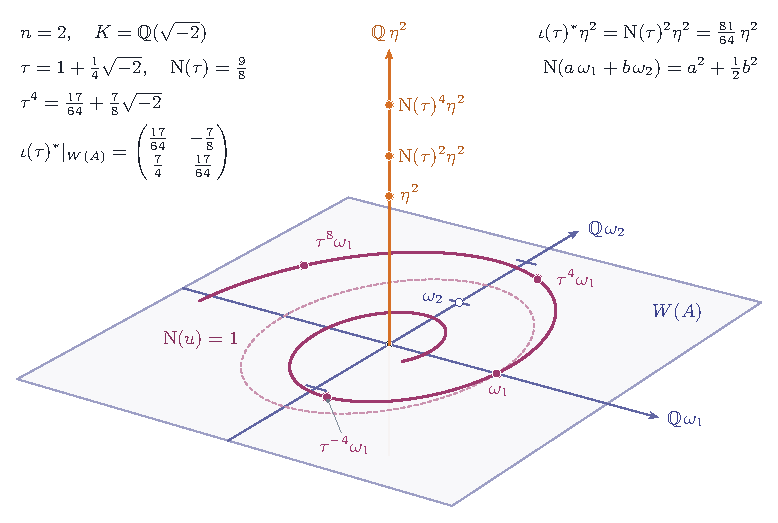
\includegraphics[width=0.96\textwidth]{fig_chernline}
\caption{The linear algebra behind \Cref{thm:divisor}, drawn inside
$H^{2n}(A,\QQ)$. The Weil line $W(A)$ is a plane, free of rank one over $K$
and of rank two over $\QQ$, and $\Kx$ acts on it through $\tau^{2n}$, so the
orbit of any nonzero class is a spiral that spans the plane and lies on no
line in it. The transverse axis carries $\eta^{n}$, on which $\Kx$ acts
through the norm. A construction returning a single eigenclass returns a
line, and by \Cref{prop:orbitplane} no line inside $W(A)$ is stable.}
\label{fig:route}
\end{figure}

\section{Secant numerology}\label{sec:numerology}

The obstructions of \Cref{thm:divisor,thm:character} concern where a class
can lie in cohomology, and neither of them uses a count of dimensions. A
secant construction is also subject to such a count, and this section shows
that the count obstructs nothing. It asks for a polarisation on $\Av$ whose
Euler characteristic lies below the values at which the theorem of Lefschetz
guarantees that a linear system is free of base points or very ample. Those
values are sufficient conditions and not necessary ones, and already on
abelian surfaces there are base-point-free and very ample systems below them.

\subsection{The dimension count}

\begin{setupenv}[The secant numerology]\label{setup:numerology}
Let $A$ be of $(K,-1,n)$-Weil type, so that $\dim A=\dim\Av=2n$. Suppose that
$\Av$ is embedded in $\PP^{N-1}$ by a complete linear system $|M|$ with $M$
ample. An ample line bundle on an abelian variety has no higher cohomology,
so $N=h^{0}(M)=\chi(M)$. The $n$-th secant variety of a nondegenerate
$2n$-fold has expected dimension
\[
  \dim\Sec^{n}(\Av)=n(2n+1)-1=2n^{2}+n-1,
\]
and for a construction that intersects $\Sec^{n}(\Av)$ with $\Av$ in the
expected dimension inside $\PP^{N-1}$,
\[
  \dim\bigl(\Sec^{n}(\Av)\cap\Av\bigr)
  =\bigl(2n^{2}+n-1\bigr)+2n-\bigl(N-1\bigr)
  =2n^{2}+3n-N .
\]
Requiring this dimension to be $n$, so that the construction produces a class
of the required codimension, forces
\begin{equation}\label{eq:chirequired}
  N=\chi(M)=2n^{2}+2n .
\end{equation}
\end{setupenv}

\begin{lemma}\label{lem:chicompare}
For every $n\ge2$,
\[
  2n^{2}+2n<2^{2n}<3^{2n},
\]
and the ratio $2^{2n}/(2n^{2}+2n)$ tends to infinity.
\end{lemma}

\begin{proof}
The right inequality is clear. Since $2^{2n}=4^{n}$, put
$q(n)=4^{n}/(2n^{2}+2n)$, so that $q(2)=16/12>1$. The ratio of consecutive
values is
\[
  \frac{q(n+1)}{q(n)}=\frac{4(2n^{2}+2n)}{2(n+1)^{2}+2(n+1)}=\frac{4n}{n+2},
\]
which is at least $2$ for $n\ge2$. Hence $q(n)\ge2^{\,n-2}q(2)>1$ for every
$n\ge2$, and $q(n)\to\infty$.
\end{proof}

\subsection{The Lefschetz thresholds}

The theorem of Lefschetz says that for $M$ ample on an abelian variety,
$M^{\otimes2}$ is free of base points and $M^{\otimes3}$ is very ample
\cite[Section~4.5]{BL04}. If $M=P^{\otimes2}$ with $P$ ample on an abelian
variety of dimension $m$, then $\chi(M)=2^{m}\chi(P)\ge2^{m}$, since
$\chi(L)=(L^{m})/m!$ for every line bundle $L$ by Riemann--Roch, and similarly
$\chi\ge3^{m}$ in the very ample case. Read as thresholds, these bounds would
say that there is no base-point-free system below $2^{m}$ and no very ample
system below $3^{m}$. Both readings turn a sufficient condition into a
necessary one, and both fail already for abelian surfaces.

\begin{proposition}[The thresholds are not necessary]\label{prop:thresholds}
Let $S$ be a general complex abelian surface, so $m=2$.
\begin{enumerate}[label=\textup{(\roman*)},nosep]
\item A polarisation of type $(1,3)$ on $S$ has $\chi=3<4=2^{2}$ and its
  complete linear system is free of base points; the associated morphism
  $S\to\PP^{2}$ is a six-sheeted covering.
\item A polarisation of type $(1,5)$ on $S$ has $\chi=5<9=3^{2}$ and is very
  ample; the image is a Horrocks--Mumford abelian surface of degree $10$ in
  $\PP^{4}$ \textup{\cite{HM73}}.
\end{enumerate}
In particular neither $2^{m}$ nor $3^{m}$ is a lower bound for the Euler
characteristic of a base-point-free, respectively very ample, ample line
bundle on an abelian variety of dimension $m$.
\end{proposition}

\begin{proof}
By Riemann--Roch on an abelian surface, a polarisation $L$ of type $(1,d)$
has $\chi(L)=(L^{2})/2=d$. The remaining assertions belong to the
classification of $(1,d)$-polarised abelian surfaces; see Gross and Popescu
\cite[\S1.2]{GP98}, where the base locus of $|L|$ is determined for each $d$:
it is empty for $d\ge3$, consists of four points for $d=2$, and $|L|$ is very
ample for $d\ge5$ on a general surface, the case $d=5$ being the
Horrocks--Mumford embedding of \cite{HM73}. In that case the image has degree
$(L^{2})=10$. For $d=3$ the morphism $S\to\PP^{2}$ defined by $|L|$ contracts
no curve, because $L$ is ample, so it is finite and surjective, of degree
$(L^{2})=6$.
\end{proof}

\begin{corollary}\label{cor:nonumerical}
The count of \Cref{setup:numerology} leads to no contradiction. The
requirement $\chi(M)=2n^{2}+2n$ of \eqref{eq:chirequired} is compatible with
$M$ being very ample for all $n$ for which a polarisation of that Euler
characteristic and suitable type exists on a $2n$-dimensional abelian
variety. At $n=2$ the requirement $\chi=12$ on an abelian fourfold is met by
polarisations of type $(1,1,2,6)$ and $(1,1,1,12)$, and nothing in the
numerology excludes very ampleness for either.
\end{corollary}

\begin{remark}[The threshold reading]\label{rem:retract}
The supplementary material of the preprint cited on the title page asserts that the polarisation required by \eqref{eq:chirequired} admits no
base-point-free linear system, on the basis of a table of the values
$2n^{2}+2n$, $2^{2n}$ and $3^{2n}$. The table is correct, and
\Cref{lem:chicompare} reproduces it, but by \Cref{prop:thresholds} the
inference drawn from it does not hold, and the claim is withdrawn. The obstructions of
\Cref{thm:divisor,thm:character} are of a different nature: they bound where
a class can lie in a decomposition of cohomology, and no choice of
polarisation, ambient space or object affects them.
\end{remark}

\section{The semiregularity target}\label{sec:semireg}

Markman's construction at $n=2$ deforms a sheaf across a family and controls
the obstruction by a semiregularity argument in the sense of Bloch and of
Buchweitz and Flenner \cite{Blo72,BF03}. As for the secant construction of
\Cref{sec:numerology}, one may ask whether a dimension count blocks this route
for $n\ge4$. We compute the target of the semiregularity map and show that it
grows too fast for the count to impose any such constraint, so that neither
route meets a numerical obstruction. The constraint that does exist is
structural. In \Cref{ssec:rankzero} we show that the annihilator of the Weil
line in $H^{0,2}(A)$ has dimension $n^{2}$, and that it prevents every object
whose Chern character is concentrated on the Weil line from being
semiregular as soon as $H^{2}(\cO_{A})$ acts on the object faithfully. In
\Cref{ssec:tangent} we identify this annihilator with the tangent space to the
Weil family.

\subsection{The dimension of the target}

\begin{lemma}[Hodge numbers of an abelian variety]\label{lem:hodgenumbers}
For an abelian variety $A$ of dimension $g$ one has
$h^{p,q}(A)=\binom{g}{p}\binom{g}{q}$.
\end{lemma}

\begin{proof}
By \eqref{eq:wedge} and the compatibility of the Hodge decomposition with the
exterior algebra structure,
$H^{p,q}(A)=\bigwedge^{p}H^{1,0}\otimes\bigwedge^{q}H^{0,1}$, and
$\dim H^{1,0}=\dim H^{0,1}=g$.
\end{proof}

\begin{proposition}[The semiregularity target]\label{prop:target}
Let $A$ be an abelian variety of dimension $g=2n$. The target of the
semiregularity map, namely $\bigoplus_{q}H^{q+2}(A,\Omega^{q}_{A})$, has
dimension
\[
  \sum_{q\ge0}h^{q,q+2}(A)=\binom{4n}{2n-2}.
\]
\end{proposition}

\begin{proof}
By \Cref{lem:hodgenumbers} with $g=2n$,
\[
  \sum_{q\ge0}h^{q,q+2}
  =\sum_{q\ge0}\binom{2n}{q}\binom{2n}{q+2}
  =\sum_{q\ge0}\binom{2n}{q}\binom{2n}{2n-q-2}
  =\binom{4n}{2n-2},
\]
the last step being the Vandermonde convolution.
\end{proof}

\begin{corollary}[The dimension count]\label{cor:countnotbind}
The target dimension $\binom{4n}{2n-2}$ takes the values
$28,495,8008,125970,1961256,30421755$ for $n=2,\dots,7$, growing by a factor
exceeding ten at each step. Any source whose dimension grows polynomially in
$n$, for instance the quadratic quantity $\binom{2n}{2}=n(2n-1)$, which takes
the values $6,15,28,45,66,91$ over the same range, is eventually negligible
against it. In particular, for large $n$ a comparison of the two dimensions
cannot obstruct the existence of a semiregular sheaf; the inequality it
produces points the other way.
\end{corollary}

\begin{remark}[Consistency at $n=2$]\label{rem:markmanconsistent}
At $n=2$ the target has dimension $28$, and the sheaf produced by Markman has
$\dim\Ext^{2}=12$, well below it, which is consistent with the construction
succeeding there. Nothing in the numbers changes character between $n=2$ and
$n=4$, so if the construction cannot be carried out for larger $n$, the reason
is not this comparison.
\end{remark}

\begin{remark}[The remaining requirement]\label{rem:semiregneed}
\Cref{cor:countnotbind} does not show that the semiregularity route works.
It removes one apparent obstruction and leaves the actual requirement in
place, namely the construction of a sheaf on $A$ whose Chern character has a
nonzero component along the Weil line. By \Cref{thm:character} such a sheaf
cannot be $K$-equivariant with the norm character, so it cannot be produced
by any functorial construction from $K$-invariant data on $\Av$; Markman's
sheaf at $n=2$ is not produced in this way. In this sense the problem for
$n\ge3$ is one of breaking equivariance, and the dimensions play no role in
it.
\end{remark}

\subsection{The annihilator of the Weil line and objects of rank zero}
\label{ssec:rankzero}

By \Cref{rem:semiregneed}, what remains is to construct a sheaf whose Chern
character has a component along the Weil line. The most economical way to
arrange this is to make the Chern character lie \emph{entirely} on the Weil
line, that is, to take an object of rank zero with every $\ch_{k}$ vanishing
except $\ch_{n}$, as the construction of \Cref{sec:construction} does. We show
that this choice is incompatible with semiregularity whenever $H^{2}(\cO_{A})$
acts faithfully on the object, for a reason that depends only on the position
of the Chern character and not on how the object is built.

We first recall the semiregularity map, on which the rest of this subsection
turns. For a coherent sheaf $\cE$ on a smooth projective variety $A$ the semiregularity
map is defined through the Atiyah class
$\mathrm{At}(\cE)\in\Ext^{1}(\cE,\cE\otimes\Omega^{1}_{A})$: a class
$\xi\in\Ext^{2}(\cE,\cE)$ is sent to the trace of
$\xi\cdot\exp(\mathrm{At}(\cE))$, and the component of that trace in
$H^{q+2}(A,\Omega^{q}_{A})=H^{q,q+2}(A)$ is the $q$-th coordinate of
$\sigma_{\cE}(\xi)$. Bloch introduced the map for local complete
intersections \cite{Blo72}, and Buchweitz and Flenner extended it to
arbitrary coherent sheaves and perfect complexes \cite{BF03}. If $A$ moves in
a family $\cA\to S$, the obstruction to extending $\cE$ to first order along
$v\in T_{s}S$ is a class $\mathrm{ob}_{v}(\cE)\in\Ext^{2}(\cE,\cE)$, and the
theorem of Buchweitz and Flenner identifies $\sigma_{\cE}(\mathrm{ob}_{v}(\cE))$
with the derivative of $\ch(\cE)$ in the direction $v$, projected off the
diagonal of the Hodge decomposition. Hence if $\ch(\cE)$ stays of Hodge type
along $S$, then $\sigma_{\cE}(\mathrm{ob}_{v}(\cE))=0$, and if $\sigma_{\cE}$ is
also injective, then $\mathrm{ob}_{v}(\cE)=0$ and $\cE$ deforms.
Injectivity thus converts a statement about the Chern character into a
statement about the sheaf, and it is the one hypothesis in the argument that
sees more than $\ch(\cE)$.

Two special cases are all that is needed below. For a line bundle $L$ one has
$\Ext^{2}(L,L)=H^{2}(\cO_{A})=H^{0,2}(A)$, and $\sigma_{L}$ is multiplication
by $e^{c_{1}(L)}$. For a direct sum, $\Ext^{2}$ is the sum of the
$\Ext^{2}(\cE_{i},\cE_{j})$, and $\sigma$ acts on each diagonal block
$H^{2}(\cO_{A})\cdot\id_{\cE_{i}}$ by multiplication by the Chern character of
that summand. Both formulae follow at once from the definition by the trace.

\begin{lemma}[The annihilator of the Weil line in $H^{0,2}$]
\label{lem:annihilator}
Let $A$ be of $(K,-1,n)$-Weil type and let $\omega\in\HW(A)\otimes\RR$ be
any nonzero real element of the Weil line. Then the multiplication map
\[
  H^{0,2}(A)\longrightarrow H^{n,n+2}(A),\qquad z\longmapsto z\cdot\omega,
\]
has kernel of dimension exactly $n^{2}$, spanned by the products $u\wedge v$
with $u\in V_{+}^{0,1}$ and $v\in V_{-}^{0,1}$. In particular the kernel is
the same subspace for every $\omega$ on the line.
\end{lemma}

\begin{proof}
Write $\omega=a\,\alpha_{+}+b\,\alpha_{-}$ with $\alpha_{\pm}$ generating
$\bigwedge^{2n}V_{\pm}$, which is possible because
$\HW(A)\otimes\CC=\bigwedge^{2n}V_{+}\oplus\bigwedge^{2n}V_{-}$ (see the proof
of \Cref{prop:weilline}). Complex conjugation interchanges $V_{+}$ and
$V_{-}$, so $\bbar{\alpha}_{+}=\mu\,\alpha_{-}$ for some $\mu\ne0$, and
comparing $\omega$ with $\bbar{\omega}=\omega$ gives $b=\bbar{a}\,\mu$. Since
$\omega\ne0$, the coefficients $a$ and $b$ are therefore both nonzero. As
$H^{0,1}=V_{+}^{0,1}\oplus V_{-}^{0,1}$ with each summand of dimension $n$,
the space $H^{0,2}=\bigwedge^{2}H^{0,1}$ decomposes as
\[
  H^{0,2}
  =\textstyle\bigwedge^{2}V_{+}^{0,1}
  \;\oplus\;\bigl(V_{+}^{0,1}\otimes V_{-}^{0,1}\bigr)
  \;\oplus\;\bigwedge^{2}V_{-}^{0,1},
\]
of dimensions $\binom{n}{2}$, $n^{2}$ and $\binom{n}{2}$.
For $u\in V_{+}^{0,1}$ and $v\in V_{-}^{0,1}$ the mixed product $u\wedge v$
satisfies $u\wedge v\wedge\alpha_{+}=0$, because $u\wedge\alpha_{+}$ lies in
$\bigwedge^{2n+1}V_{+}=0$, and $u\wedge v\wedge\alpha_{-}=0$ for the same
reason with $v$. So the middle summand lies in the kernel.

Conversely, let $z=z_{++}+z_{+-}+z_{--}$ be in the kernel. For the same
reason $z_{++}\wedge\alpha_{+}$, $z_{--}\wedge\alpha_{-}$ and
$z_{+-}\wedge\omega$ vanish, so
$z\cdot\omega=a\,z_{--}\wedge\alpha_{+}+b\,z_{++}\wedge\alpha_{-}$. If $n=1$
the outer summands are zero and there is nothing to prove. If $n\ge2$ the two
terms lie in the distinct summands
$\bigwedge^{2n}V_{+}\otimes\bigwedge^{2}V_{-}$ and
$\bigwedge^{2}V_{+}\otimes\bigwedge^{2n}V_{-}$ of
$\bigwedge^{2n+2}V_{\CC}=\bigwedge^{2n+2}(V_{+}\oplus V_{-})$, so each of them
vanishes. Wedging with a generator of $\bigwedge^{2n}V_{+}$ is injective on
$\bigwedge^{2}V_{-}$, and wedging with a generator of $\bigwedge^{2n}V_{-}$ is
injective on $\bigwedge^{2}V_{+}$. Since $a\neq0$ we get $z_{--}=0$, and since
$b\neq0$ we get $z_{++}=0$, so the kernel is the middle summand.
\end{proof}

The reality of $\omega$ is needed: for the non-real element
$\omega=\alpha_{+}$ of $\HW(A)\otimes\CC$ the same computation gives the
kernel $V_{+}^{0,1}\otimes V_{-}^{0,1}\oplus\bigwedge^{2}V_{+}^{0,1}$, of
dimension $n^{2}+\binom{n}{2}$. \Cref{fig:fibres} draws the mixed block that forms the kernel.

\begin{theorem}[The rank-zero obstruction]
\label{thm:rankzero}
Let $A$ be of $(K,-1,n)$-Weil type. Let $\cE_{1}$ and $\cE_{2}$ be coherent
sheaves on $A$ such that
\[
  \ch(\cE_{1})-\ch(\cE_{2})=c\,\omega,\qquad c\neq0,\quad \omega\in\HW(A),
\]
such that $\Ext^{2}(\cE_{1},\cE_{2})=\Ext^{2}(\cE_{2},\cE_{1})=0$, and such
that the map $H^{2}(\cO_{A})\to\Ext^{2}(\cE_{1},\cE_{1})$,
$z\mapsto z\cdot\id_{\cE_{1}}$, is injective, as it is whenever
$\rk\cE_{1}\neq0$. Put $\cE=\cE_{1}\oplus\cE_{2}$. Then the semiregularity
map
\[
  \sigma_{\cE}\colon\ \Ext^{2}(\cE,\cE)\longrightarrow\bigoplus_{q\ge0}H^{q,q+2}(A)
\]
has kernel of dimension at least $n^{2}$. In particular $\cE$ is not
semiregular, for any $n\ge1$.
\end{theorem}

\begin{proof}
The vanishing of the off-diagonal $\Ext^{2}$ groups gives
$\Ext^{2}(\cE,\cE)=\Ext^{2}(\cE_{1},\cE_{1})\oplus\Ext^{2}(\cE_{2},\cE_{2})$,
and each summand receives $H^{2}(\cO_{A})$ through the $\cO_{A}$-module
structure, $z\mapsto z\cdot\id_{\cE_{i}}$. For $z\in H^{2}(\cO_{A})=H^{0,2}(A)$
consider the element $\xi_{z}=z\cdot\id_{\cE_{1}}-z\cdot\id_{\cE_{2}}$. Its
component in $\Ext^{2}(\cE_{1},\cE_{1})$ is $z\cdot\id_{\cE_{1}}$, so by
hypothesis $z\mapsto\xi_{z}$ is injective. The semiregularity map is
compatible with direct sums, and on $H^{0,2}\cdot\id_{\cE_{i}}$ it is
multiplication by the Chern character of $\cE_{i}$, so
\[
  \sigma_{\cE}(\xi_{z})=z\cdot\ch(\cE_{1})-z\cdot\ch(\cE_{2})
  =c\,z\cdot\omega .
\]
If $\omega=0$ this vanishes for every $z$, and
$\dim H^{0,2}=n(2n-1)\ge n^{2}$. Otherwise $\omega$, being rational, is a
nonzero real element of the Weil line, and by \Cref{lem:annihilator} the
product vanishes for every $z$ in an $n^{2}$-dimensional subspace of
$H^{0,2}$. The corresponding $\xi_{z}$ are linearly independent, and hence
$\dim\ker\sigma_{\cE}\ge n^{2}$.

It remains to justify the claim in the statement that the hypothesis on
$\cE_{1}$ holds in positive rank. For a coherent sheaf $\cF$ the map
$H^{2}(\cO_{A})\to\Ext^{2}(\cF,\cF)$, $z\mapsto z\cdot\id_{\cF}$, is the edge
map of the local-to-global spectral sequence, and
$\operatorname{tr}(z\cdot\id_{\cF})=\rk(\cF)\,z$. When $\rk\cF\ne0$ the trace
therefore splits the map up to the factor $\rk\cF$, and the map is
injective; this applies in particular to a direct sum of line bundles. For a
sheaf of rank zero the map can vanish: for a skyscraper sheaf it factors
through $H^{2}$ of the structure sheaf of a point, which is zero. The direct
sum $\cE_{1}\oplus\cE_{2}$ is used only to produce an element of $\Ext^{2}$
whose image under $\sigma$ is $z\cdot(\ch\cE_{1}-\ch\cE_{2})$ rather than
$z\cdot(\ch\cE_{1}+\ch\cE_{2})$.
\end{proof}

\begin{corollary}[The construction of \Cref{sec:construction}]
\label{cor:pteobstructed}
Let $L_{1},\dots,L_{m}$ be line bundles on $A$ with
$\sum_{i}c_{1}(L_{i})=0$ such that the virtual class
$\sum_{i}\bigl([L_{i}]-[L_{i}^{-1}]\bigr)$ has Chern character on the Weil
line and every difference
$\varepsilon\,c_{1}(L_{i})-\varepsilon'c_{1}(L_{j})$ with
$\varepsilon,\varepsilon'\in\{\pm1\}$ and $(\varepsilon,i)\ne(\varepsilon',j)$
is nondegenerate of index different from $2$. Then the sheaf
$\bigoplus_{i}(L_{i}\oplus L_{i}^{-1})$ has semiregularity kernel of
dimension at least $n^{2}$. At $n=3$ the explicit object of
\Cref{sec:construction} has kernel of dimension exactly
$15=n^{2}+n(n-1)$, of which the $n^{2}=9$ dimensions on the odd side are
the ones supplied by \Cref{thm:rankzero}; the remaining $n(n-1)=6$ come from
the even side and are specific to the line-bundle structure.
\end{corollary}

\begin{proof}
Take $\cE_{1}=\bigoplus L_{i}$ and $\cE_{2}=\bigoplus L_{i}^{-1}$. Then
$\Ext^{2}(\cE_{1},\cE_{2})=\bigoplus_{i,j}H^{2}(L_{i}^{-1}\otimes L_{j}^{-1})$
and $\Ext^{2}(\cE_{2},\cE_{1})=\bigoplus_{i,j}H^{2}(L_{i}\otimes L_{j})$, and
the first Chern classes $\mp\bigl(c_{1}(L_{i})+c_{1}(L_{j})\bigr)$ occurring
here, for all $i$ and $j$, are differences of the kind in the hypothesis,
with $\varepsilon'=-\varepsilon$. A nondegenerate line bundle has cohomology only in
the degree equal to its index, so the index hypothesis gives the required
$\Ext^{2}$ vanishing. The sheaf $\cE_{1}$ has rank $m\ne0$, and the Chern
character hypothesis is that of \Cref{thm:rankzero}.
Since $e^{\lambda}$ and $e^{-\lambda}$ combine into $\cosh\lambda$ and
$\sinh\lambda$, which occupy disjoint degrees, the map splits by parity, and
the odd part is the annihilator of \Cref{lem:annihilator} tensored with the
sign vector. At $n=3$ the dimensions are read off from the proof of
\Cref{prop:explicitobject}, where the signs are absorbed in the same way:
the kernel consists of the vectors $(u_{i}^{-k}z)_{i}$ with $z$ in the mixed
block $V_{+}^{0,1}\otimes V_{-}^{0,1}$ for $k=3$, which change sign under
$u_{i}\mapsto-u_{i}$, and with $z$ in $\bigwedge^{2}V_{+}^{0,1}$ or
$\bigwedge^{2}V_{-}^{0,1}$ for $k=2$ or $k=4$, which do not.
\end{proof}

\begin{remark}[Uniformity over the configurations]
\label{rem:familyuniform}
By \Cref{cor:pteobstructed} the kernel has dimension at least $n^{2}$ for
every configuration of line bundles $L_{i}^{\pm1}$ whose virtual Chern
character lies on the Weil line and whose differences are nondegenerate of
index different from $2$. The deficiency is therefore not special to the six
line bundles of \Cref{prop:explicitobject}: \Cref{thm:rankzero} produces it
from the vanishing of the rank alone.

\Cref{thm:rankzero} excludes the economical choice described at the start of
this subsection. An object on which $H^{2}(\cO_{A})$ acts faithfully and which
realises a Weil class through semiregularity cannot have its Chern character
concentrated on the Weil line. It must carry a nonzero rank, or nonzero Chern
character in other degrees, so that $z\mapsto z\cdot\ch(\cE)$ is injective on
$H^{0,2}$; the degree-two component of that product is $\rk(\cE)\cdot z$, and
rank zero is the case in which it vanishes. Markman's sheaves have nonzero
rank, and this is essential to his method: the class he shows to be
deformation-invariant is the normalised character
$\exp(-c_{1}(\cE)/\rk\cE)\ch(\cE)$, which divides by the rank, and the objects
at $n=3$ are reflexive sheaves \cite{Mar25a,Mar25b}. This narrows the fourth
ingredient of \Cref{rem:deformation}: it is a single sheaf of positive rank
whose Chern character has a Weil component alongside other components, rather
than a difference of two sheaves whose classes cancel outside the Weil line.
\end{remark}

\Cref{thm:rankzero} is stated for a direct sum because there the element
$\xi_{z}$ is explicit. The mechanism applies to any perfect complex on which
$H^{2}(\cO_{A})$ acts faithfully, and in particular to the object used in
\Cref{sec:reduction}.

\begin{proposition}[Complexes with concentrated Chern character]
\label{prop:concentrated}
Let $A$ be of $(K,-1,n)$-Weil type and let $E$ be a nonzero perfect complex on
$A$ with $\ch_{k}(E)=0$ for $k\ne n$ and $\ch_{n}(E)=N\omega$ for some
$N\ne0$ and some nonzero $\omega\in\HW(A)$. If the natural map
\begin{equation}\label{eq:idmap}
  H^{2}(\cO_{A})\longrightarrow\Ext^{2}(E,E),\qquad z\longmapsto z\cdot\id_{E},
\end{equation}
is injective, then $\dim\ker\sigma_{E}\ge n^{2}$, so $E$ is not semiregular.
The map \eqref{eq:idmap} is injective whenever $E$ is represented by a virtual
sum of line bundles, in particular at every base point of
\Cref{cor:splitalgebraic}, \Cref{thm:quatweil} and \Cref{thm:everyn}.
\end{proposition}

\begin{proof}
For any perfect complex the semiregularity map satisfies
$\sigma_{E}(z\cdot\id_{E})=z\cdot\ch(E)$, since
$\operatorname{tr}\bigl(z\cdot\id_{E}\circ\exp\mathrm{At}(E)\bigr)
=z\cdot\operatorname{tr}\exp\mathrm{At}(E)=z\cdot\ch(E)$. Hence for $z$ in the
annihilator of $\omega$ in $H^{0,2}(A)$,
\[
  \sigma_{E}(z\cdot\id_{E})=N\,z\cdot\omega=0 ,
\]
and that annihilator has dimension $n^{2}$ by \Cref{lem:annihilator}. If
\eqref{eq:idmap} is injective, the classes $z\cdot\id_{E}$ for $z$ in a basis
of the annihilator are linearly independent, which gives the bound.

For the last sentence, write the class of $E$ in $K_{0}(A)$ as
$\sum_{i}\varepsilon_{i}[L_{i}]$ with $\varepsilon_{i}=\pm1$ and $L_{i}$ line
bundles, and realise it by the direct sum of the $L_{i}$ with
$\varepsilon_{i}=1$ and of the shifts $L_{i}[1]$ of those with
$\varepsilon_{i}=-1$. The map \eqref{eq:idmap} is then $z\mapsto(z,\dots,z)$
into $\bigoplus_{i}\Ext^{2}(L_{i},L_{i})=\bigoplus_{i}H^{2}(\cO_{A})$, which is
injective. At a split member $\omega_{1}$ is a polynomial in
$\beta,\widehat\beta,\ell$ by \Cref{thm:splitclosed}(iii), at a quaternionic
member it is a polynomial in divisor classes by \Cref{thm:quatweil}, and at a
product it is one by \Cref{thm:everyn}; in each case the Chern character is a
ring expression in classes of line bundles, so such a representation exists.
\end{proof}

\begin{proposition}[The class forces the size of the object]%
\label{prop:objectsize}
Let $A$ be of $(K,-1,n)$-Weil type, let $\omega$ be a nonzero element of the
Weil line and let $E$ be a perfect complex on $A$ with
\[
  \ch(E)=r+N\omega,\qquad r\in H^{0}(A,\QQ),\ N\ne0,
\]
and no other component. Then
\[
  \chi(E,E)\;=\;(-1)^{n}N^{2}\!\int_{A}\omega^{2},
\]
independently of $r$, and consequently
\[
  \sum_{i}\dim\Ext^{i}(E,E)\;\ge\;N^{2}\Bigl|\int_{A}\omega^{2}\Bigr|\;>\;0 .
\]
\end{proposition}

\begin{proof}
The Todd class of an abelian variety is $1$, so Riemann--Roch for the Ext
algebra reads $\chi(E,E)=\int_{A}\ch(E)^{\vee}\ch(E)$ with
$\ch_{k}^{\vee}=(-1)^{k}\ch_{k}$. Expanding,
\[
  \ch(E)^{\vee}\ch(E)
  = r^{2}+\bigl(1+(-1)^{n}\bigr)rN\omega+(-1)^{n}N^{2}\omega^{2},
\]
and of the three terms only the last has degree $4n$, so only it survives the
integral; the rank enters solely through $r^{2}$, which sits in degree zero.
For the inequality, $\chi(E,E)=\sum_{i}(-1)^{i}\dim\Ext^{i}(E,E)$, so the
total dimension is at least $|\chi(E,E)|$. Finally $\int_{A}\omega^{2}\ne0$.
Write $\omega=\alpha_{+}+\alpha_{-}$ with $\alpha_{\pm}\in\bigwedge^{2n}V_{\pm}$,
both nonzero by the proof of \Cref{lem:annihilator}. Each $\alpha_{\pm}$ is a
top form on its own eigenspace and squares to zero, so
$\omega^{2}=2\alpha_{+}\alpha_{-}$, which is a nonzero multiple of the
fundamental class.
\end{proof}

\begin{remark}[The constant]\label{rem:sizeconstant}
The bound concerns the whole Ext algebra and does not depend on the rank, so
increasing the rank does not weaken it. The constant $|\int\omega^{2}|$
depends on the normalisation of $\omega$; measured against $\eta$ it picks up
factors of $d$ and of the polarisation type, and no dimension-free growth
rate can be read off from it. The bound uses only that the Weil class is not
isotropic. Together with \Cref{prop:concentrated} it constrains an object
carrying the class in two ways. If the Chern character is concentrated on the
Weil line, the semiregularity map has a kernel of dimension at least $n^{2}$
unless $H^{2}(\cO_{A})$ acts on the object degenerately; and whatever the
rank, the Ext algebra has dimension at least $N^{2}|\int\omega^{2}|$.
\end{remark}

\begin{remark}[Consequences for the semiregularity reduction]
\label{rem:killsreduction}
\Cref{thm:semiregclosure} proves $\Sigma=\cD_{n,n}$, that is, the
algebraicity of the Weil class on the whole family, under the hypothesis that
$\sigma_{E}$ is injective for the complex $E$ of \Cref{prop:ktheory}, whose
Chern character is $N\omega_{1}$ in degree $n$ and zero elsewhere. This
complex satisfies the hypotheses of \Cref{prop:concentrated} at every base
point of \Cref{cor:splitalgebraic}, \Cref{thm:quatweil} and
\Cref{thm:everyn}, so there the hypothesis of \Cref{thm:semiregclosure} fails
for it, by $n^{2}$ dimensions.

This does not make \Cref{thm:semiregclosure} vacuous, for two reasons. First,
the hypothesis concerns a chosen perfect complex representing a class in
$K_{0}(A)_{\QQ}$, and distinct representatives of one class have distinct
$\Ext^{2}$ groups; what is ruled out is the representative that the
construction supplies. Second, \Cref{prop:concentrated} needs
\eqref{eq:idmap} to be injective, which is a real restriction for an object
of rank zero: it fails, for instance, for a sheaf supported at a point. A
representative escaping \Cref{prop:concentrated} must therefore
receive $H^{2}(\cO_{A})$ non-injectively, which for a rank-zero object means
that its support is degenerate. Of the two reductions of
\Cref{sec:reduction}, the degree bound of \Cref{thm:degreebound} is untouched
by anything here, and the semiregularity reduction of
\Cref{thm:semiregclosure} is unavailable for the complexes that the
constructions at these base points supply.
\end{remark}

\begin{figure}[t]
\centering
  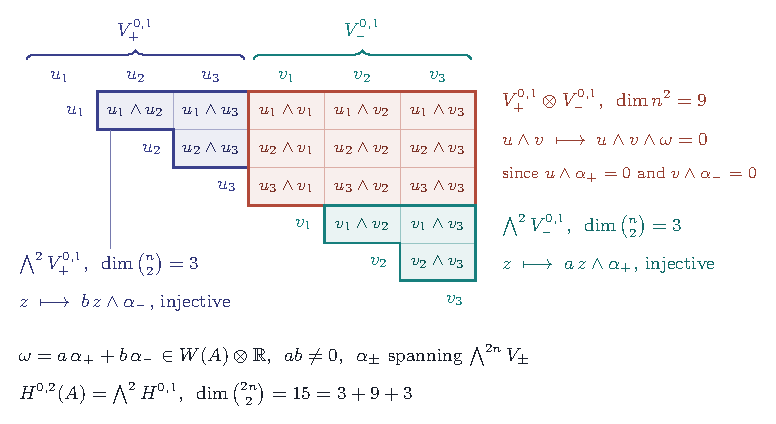
\includegraphics[width=0.94\textwidth]{fig_annihilator}
\caption{The structure behind \Cref{lem:annihilator}, drawn at $n=3$.
$H^{0,2}(A)=\bigwedge^{2}H^{0,1}$ splits into three blocks by how many factors
come from $V_{+}^{0,1}$ and how many from $V_{-}^{0,1}$. The two outer blocks,
of dimension $\binom{n}{2}=3$ each, are carried injectively by multiplication
with the Weil class. The middle block, of dimension $n^{2}=9$ and spanned by
the mixed products, goes to zero, because each such product repeats a factor
of $\alpha_{+}$ and a factor of $\alpha_{-}$. Its dimension $n^{2}$ is the
deficit in \Cref{prop:concentrated}.}
\label{fig:annihilator}
\end{figure}


\subsection{The annihilator and the tangent space to the family}
\label{ssec:tangent}

The number $n^{2}$ of \Cref{lem:annihilator} is also the dimension of the
Weil family. We show in this subsection that the polarisation identifies the
annihilator with the tangent space to the family, canonically and in every
dimension. Two consequences follow. First, the deficiency of the
semiregularity map at an object of rank zero cannot be removed by a better
choice of object, since it is the family itself, seen inside $H^{0,2}$.
Second, the first-order Hodge locus of the Weil line is the Weil family, so
the directions that the semiregularity map cannot see are those along which
the class stays Hodge and along which it would have to be carried.

Write $V_{\pm}$ for the two eigenspaces of $K$ on $H^{1}(A,\CC)$, each of
dimension $2n$, and
\[
  V_{\pm}^{1,0}=V_{\pm}\cap H^{1,0},\qquad
  V_{\pm}^{0,1}=V_{\pm}\cap H^{0,1},
\]
each of dimension $n$ by \Cref{lem:balanced}. Let $E$ denote the
polarisation form on $H^{1}(A,\QQ)$, extended to $H^{1}(A,\CC)$. We use
throughout that $E$ vanishes on $V_{+}\times V_{+}$ and on $V_{-}\times V_{-}$
and pairs $V_{+}$ with $V_{-}$ perfectly, which is condition (iii) of
\Cref{def:weiltype} read on the eigenspaces, and that $E$ vanishes on
$H^{1,0}\times H^{1,0}$ and on $H^{0,1}\times H^{0,1}$, which is the first
Riemann bilinear relation. For the first statement, let $x,y\in V_{+}$. Then
$E(\sqrt{-d}\,x,y)=\sqrt{-d}\,E(x,y)$ from the eigenvalue, and
$E(\sqrt{-d}\,x,y)=-E(x,\sqrt{-d}\,y)=-\sqrt{-d}\,E(x,y)$ from
\Cref{def:weiltype}(iii), so $E(x,y)=0$. The same holds on $V_{-}$, and the
nondegeneracy of $E$ then forces the pairing between $V_{+}$ and $V_{-}$ to
be perfect. Together, the two vanishing statements say that of the four
blocks of $E$ on
$(V_{+}^{1,0}\oplus V_{+}^{0,1})\times(V_{-}^{1,0}\oplus V_{-}^{0,1})$ only
$V_{+}^{1,0}\times V_{-}^{0,1}$ and $V_{+}^{0,1}\times V_{-}^{1,0}$ are
nonzero, and each of these two is a perfect pairing of $n$-dimensional
spaces. This block structure is all that the proof of \Cref{thm:anntangent}
uses of $E$.

A first-order deformation of $A$ is a class in $H^{1}(A,T_{A})$, which for an
abelian variety is canonically $\Hom(H^{1,0},H^{0,1})$, since the tangent
bundle is trivial and $H^{1,0}$ is the dual of its space of sections. Such a
$v$ is extended to $H^{1}(A,\CC)$ by zero on $H^{0,1}$ and acts on
$H^{k}(A,\CC)=\bigwedge^{k}H^{1}(A,\CC)$ as the derivation it generates; we
write $v\lrcorner\,\xi$ for that action. A Hodge class $\xi$ of type $(p,p)$
remains of type $(p,p)$ to first order along $v$ exactly when
$v\lrcorner\,\xi=0$. We call $v$ \emph{polarised} when
$E(vx,y)+E(x,vy)=0$ for all $x,y\in H^{1,0}$, which is the condition that the
deformation preserve the polarisation. The polarised $v$ form a space of
dimension $n(2n+1)=\dim\cA_{2n}$.

\begin{proposition}[The first-order Hodge locus of the Weil line]
\label{prop:firstorder}
Let $A$ be of $(K,-1,n)$-Weil type and let $v$ be a polarised first-order
deformation of $A$. The following are equivalent.
\begin{enumerate}[label=\textup{(\roman*)},nosep]
\item $v\lrcorner\,\omega=0$ for every $\omega$ in the Weil line.
\item $v$ commutes with the action of $K$.
\item $v\bigl(V_{+}^{1,0}\bigr)\subseteq V_{+}^{0,1}$ and
  $v\bigl(V_{-}^{1,0}\bigr)\subseteq V_{-}^{0,1}$.
\end{enumerate}
The space of such $v$ has dimension $n^{2}$, and under
\Cref{prop:weildomain} it is the tangent space at $[A]$ to the Weil family
$\cD_{n,n}$. Each of the two rational generators of the Weil line already
cuts it out by itself.
\end{proposition}

\begin{proof}
The equivalence of (ii) and (iii) is immediate. Since $K$ acts on $V_{\pm}$
by the two scalars $\pm\sqrt{-d}$, commuting with $K$ means preserving $V_{+}$
and $V_{-}$. The extension of $v$ kills $H^{0,1}$ and takes values in
$H^{0,1}$, so preserving $V_{\pm}$ amounts to
$v(V_{\pm}^{1,0})\subseteq V_{\pm}\cap H^{0,1}=V_{\pm}^{0,1}$.

For (i) and (iii), let $\alpha_{+}$ generate $\bigwedge^{2n}V_{+}$ and write
$\alpha_{+}=e_{1}\wedge\cdots\wedge e_{2n}$ for a basis $e_{1},\dots,e_{2n}$
of $V_{+}$ adapted to $V_{+}=V_{+}^{1,0}\oplus V_{+}^{0,1}$. As a derivation,
\[
  v\lrcorner\,\alpha_{+}
  =\sum_{j=1}^{2n}e_{1}\wedge\cdots\wedge v(e_{j})\wedge\cdots\wedge e_{2n}.
\]
Split $v(e_{j})$ along $H^{1}(A,\CC)=V_{+}\oplus V_{-}$. The $V_{+}$
components contribute
$\operatorname{tr}\bigl(\pi_{+}\circ v|_{V_{+}}\bigr)\,\alpha_{+}$, and that
trace vanishes: the map $\pi_{+}\circ v|_{V_{+}}$ kills $V_{+}^{0,1}$ and
carries $V_{+}^{1,0}$ into $V_{+}^{0,1}$, so in the adapted basis its matrix
has zero diagonal blocks. Writing
$v(e_{j})_{-}=\sum_{k}c_{jk}f_{k}$ for a basis $f_{1},\dots,f_{2n}$ of
$V_{-}$, the $V_{-}$ components contribute
\[
  \sum_{j,k}\pm\,c_{jk}\;
  e_{1}\wedge\cdots\wedge\widehat{e_{j}}\wedge\cdots\wedge e_{2n}\wedge f_{k},
\]
and the $4n^{2}$ monomials appearing here are distinct members of the
standard basis of $\bigwedge^{2n}H^{1}(A,\CC)$, hence linearly independent.
So $v\lrcorner\,\alpha_{+}=0$ if and only if every $c_{jk}$ vanishes, which is
$v(V_{+})\subseteq V_{+}$. The same argument on $\alpha_{-}$ gives
$v\lrcorner\,\alpha_{-}=0$ if and only if $v(V_{-})\subseteq V_{-}$. The Weil
line spans $\bigwedge^{2n}V_{+}\oplus\bigwedge^{2n}V_{-}$ over $\CC$ by
\Cref{prop:weilline}, and each of the two rational generators of
\Cref{thm:explicitgens} has both components nonzero, so a single generator
already forces both conditions. This is (i) if and only if (iii).

For the dimension, let $v$ satisfy (iii), and write $v_{+}$ and $v_{-}$ for
its restrictions to $V_{+}^{1,0}$ and $V_{-}^{1,0}$. If $x$ and $y$ both lie
in $V_{+}^{1,0}$, then $v_{+}x$ and $y$ both lie in $V_{+}$, so both terms of
the polarisation condition vanish, and likewise if both lie in $V_{-}^{1,0}$.
For $x\in V_{+}^{1,0}$ and $y\in V_{-}^{1,0}$ the condition reads
$E(v_{+}x,y)=-E(x,v_{-}y)$. The left side is determined by $v_{+}$, and the
pairing between $V_{+}^{1,0}$ and $V_{-}^{0,1}$ is perfect, so for each $y$
there is exactly one $v_{-}y\in V_{-}^{0,1}$ satisfying this for all $x$, and
it depends linearly on $y$. Hence $v_{-}$ is determined by $v_{+}$, which may
be chosen freely, and the polarised deformations satisfying (iii) form a
space of dimension $\dim\Hom(V_{+}^{1,0},V_{+}^{0,1})=n^{2}$. By
\Cref{prop:weildomain} the family $\cD_{n,n}$ is an open subset of the
Grassmannian of $n$-planes in $V_{+}$, whose tangent space at
$V_{+}^{1,0}$ is $\Hom(V_{+}^{1,0},V_{+}/V_{+}^{1,0})=\Hom(V_{+}^{1,0},V_{+}^{0,1})$,
and the identification just made is that isomorphism.
\end{proof}

\begin{proposition}[Infinitesimal rigidity of divisor classes]%
\label{prop:rigidity}
Keep the notation above, put $P=V_{+}^{1,0}$ and $P'=V_{-}^{1,0}$ as in the
proof of \Cref{prop:weildomain}, so that $\bbar{P}=V_{-}^{0,1}$ and
$\bbar{P}'=V_{+}^{0,1}$, and write a class $\delta\in H^{1,1}$ in the four
blocks
\[
  a\ \text{on}\ P\otimes\bbar{P},\quad
  b\ \text{on}\ P'\otimes\bbar{P}',\quad
  c\ \text{on}\ P\otimes\bbar{P}',\quad
  e\ \text{on}\ P'\otimes\bbar{P},
\]
the first two carrying the norm character of $\Kx$ and the last two the
characters $\tau^{2}$ and $\bbar\tau^{\,2}$; reality makes $a$ and $b$
anti-hermitian and ties $e$ to $-\bbar{c}^{\,T}$. Identify the tangent space
$\Hom(P,\bbar{P}')$ to $\cD_{n,n}$ with the $n\times n$ matrices $V$ as in
\Cref{thm:anntangent}, and write $\operatorname{alt}$ for the alternating part
of a matrix, viewed in $\bigwedge^{2}$. Then contraction with a tangent
vector is
\begin{equation}\label{eq:phidelta}
  \Phi_{\delta}(V)
  \;=\;\bigl(\,Va+b^{T}V,\ \ \operatorname{alt}(Vc),\ \
       \operatorname{alt}(-V^{T}e)\,\bigr),
\end{equation}
with values in
$\bbar{P}'\otimes\bbar{P}\oplus\bigwedge^{2}\bbar{P}'\oplus\bigwedge^{2}\bbar{P}
=H^{0,2}$, and $\ker\Phi_{\delta}$ is the tangent space to the locus where
$\delta$ stays of type $(1,1)$. Consequently:
\begin{enumerate}[label=\textup{(\roman*)},nosep]
\item $\Phi_{\delta}=0$ if and only if $\delta$ is a real multiple of $\eta$.
  The rigid classes form a real line, which is the infinitesimal form of the
  statement that $\NS(A)_{\QQ}$ has rank one at the general member.
\item For the norm-character class with block $a$ and $b=c=e=0$,
  \[
    \dim\ker\Phi_{\delta}\;=\;n\,(n-\operatorname{rank}a),
  \]
  so such a class cuts a locus of codimension $n\operatorname{rank}a$, at
  least $n$.
\item A general class has $\ker\Phi_{\delta}=0$: to first order it
  rigidifies the family to a point.
\end{enumerate}
\end{proposition}

\begin{proof}
For \eqref{eq:phidelta}, a polarised deformation commuting with $K$ sends $P$
into $\bbar{P}'$ and $P'$ into $\bbar{P}$, and the polarisation condition
$E(vx,y)+E(x,vy)=0$ forces the second matrix to be $-V^{T}$, as in the proof
of \Cref{prop:firstorder}. Applying $v$ to the $(1,0)$ slot of each block and
collecting terms in $H^{0,2}$ gives the three displayed components; the sign
in the first comes from $\bbar{P}\wedge\bbar{P}'=-\bbar{P}'\wedge\bbar{P}$.

(i) If $\Phi_{\delta}=0$ then $\operatorname{alt}(Vc)=0$ for every $V$, which
for $n\ge2$ forces $c=0$, and likewise $e=0$. The first component gives
$Va=-b^{T}V$ for every $V$; taking $V$ to run over the matrix units shows
$a$ is a scalar $\lambda$ and $b^{T}=-\lambda$. Anti-hermitian scalars are
the purely imaginary ones, so the solutions form a real line. It contains
$\eta$, whose blocks are $a=i$, $b=-i$, and the two therefore agree.

(ii) With $b=c=e=0$ the condition is $Va=0$, that is, the rows of $V$
annihilate the column space of $a$; the solution space has dimension
$n(n-\operatorname{rank}a)$.

(iii) By (ii), the class with $a$ of rank $n$ (for instance $a=i$) and
$b=c=e=0$, which is real since $a$ is anti-hermitian, has
$\ker\Phi_{\delta}=0$. Since $\Phi_{\delta}$ depends linearly on $\delta$, the
classes with $\ker\Phi_{\delta}\ne0$ are cut out by the vanishing of the
maximal minors of $\Phi_{\delta}$ and form a proper real algebraic subset of
the real classes of type $(1,1)$, which gives (iii).
\end{proof}

\begin{remark}[The divisorial supply]\label{rem:rigiditywhy}
\Cref{prop:rigidity}(ii) explains why the divisorial supply of
\Cref{thm:divcriterion} cannot be enlarged by a better choice of class. Any
norm-character class other than a multiple of $\eta$ has
$\operatorname{rank}a\ge1$ and so cuts a locus of codimension at least $n$;
that locus is proper, and by (i) only the real multiples of $\eta$ cut
nothing. Each further class therefore yields a subvariety and never an open
set, which is \Cref{prop:divfails} with the codimension made explicit.
\end{remark}

\begin{figure}[htbp]
\centering
  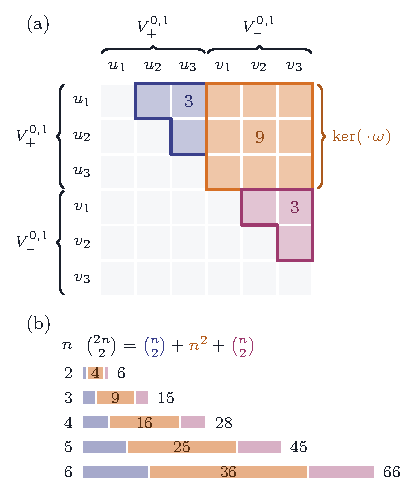
\includegraphics[width=0.46\textwidth]{fig_fibres}
\caption{The geometry behind \Cref{lem:annihilator}, drawn schematically for
the real shadow of the hermitian form. The ruled surface is the null cone of
$H$; the two transverse planes are the conjugate isotropic subspaces $V_{+}$
and $V_{-}$, which conjugation interchanges, so that neither is defined over
$\QQ$ and only their sum is. The segments join a vector of one to its
conjugate in the other, and the strip they sweep stands for the mixed block
$V_{+}^{0,1}\otimes V_{-}^{0,1}$, of dimension $n^{2}$, which multiplication
by the Weil class sends to zero and which is the deficit in
\Cref{prop:concentrated}.}
\label{fig:fibres}
\end{figure}

\begin{theorem}[The annihilator is the tangent space]\label{thm:anntangent}
Let $A$ be of $(K,-1,n)$-Weil type and let $\omega$ be a rational generator of
the Weil line. The polarisation induces an isomorphism
\[
  T_{[A]}\cD_{n,n}\;\xrightarrow{\ \sim\ }\;
  \operatorname{Ann}_{H^{0,2}(A)}(\omega),
\]
canonical in the sense that it depends on no choice of basis and on no choice
of $\omega$ on the line. Explicitly, if $p_{1},\dots,p_{n}$ is a basis of
$V_{+}^{1,0}$ and $q_{1},\dots,q_{n}$ the basis of $V_{-}^{0,1}$ dual to it
under $E$, then $\varphi\in\Hom(V_{+}^{1,0},V_{+}^{0,1})$ corresponds to
\[
  \sum_{a=1}^{n}q_{a}\wedge\varphi(p_{a})\;\in\;
  V_{-}^{0,1}\otimes V_{+}^{0,1}\;\subset\;\textstyle\bigwedge^{2}H^{0,1}
  =H^{0,2}(A).
\]
\end{theorem}

\begin{proof}
The form $E$ pairs $V_{+}$ with $V_{-}$ perfectly and vanishes on
$V_{+}^{1,0}\times V_{-}^{1,0}$, the latter because both spaces lie in
$H^{1,0}$. Hence $E$ restricted to $V_{+}^{1,0}\times V_{-}$ kills
$V_{-}^{1,0}$ and descends to a pairing
\[
  V_{+}^{1,0}\times V_{-}^{0,1}\longrightarrow\CC .
\]
This pairing is perfect: both spaces have dimension $n$, and a vector of
$V_{+}^{1,0}$ orthogonal to $V_{-}^{0,1}$ is orthogonal to all of $V_{-}$,
hence zero. It gives a canonical isomorphism
$\bigl(V_{+}^{1,0}\bigr)^{*}\cong V_{-}^{0,1}$, and therefore
\[
  T_{[A]}\cD_{n,n}
  =\Hom\bigl(V_{+}^{1,0},V_{+}^{0,1}\bigr)
  =\bigl(V_{+}^{1,0}\bigr)^{*}\otimes V_{+}^{0,1}
  \;\cong\;V_{-}^{0,1}\otimes V_{+}^{0,1},
\]
the first equality being the tangent space computation at the end of the proof
of \Cref{prop:firstorder}. Since $H^{0,1}=V_{+}^{0,1}\oplus V_{-}^{0,1}$, the
map $q\otimes u\mapsto q\wedge u$ identifies $V_{-}^{0,1}\otimes V_{+}^{0,1}$
with the middle summand of
$\bigwedge^{2}H^{0,1}$, and that summand is the annihilator by
\Cref{lem:annihilator}. The displayed formula is the composite of these
isomorphisms written in a dual pair of bases, so it is independent of the
basis chosen; and \Cref{lem:annihilator} gives the same subspace for every
$\omega$ on the line, so the isomorphism does not depend on $\omega$ either.
\end{proof}

\begin{figure}[tbp]
\centering
  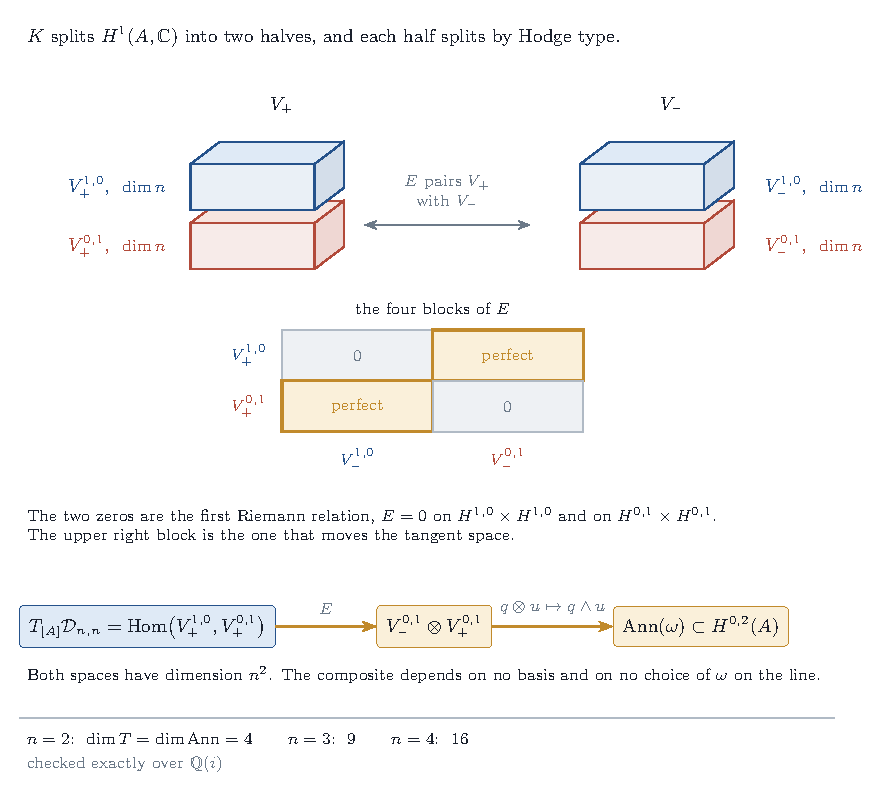
\includegraphics[width=\textwidth]{fig_tangent}
\caption{\Cref{thm:anntangent}. The polarisation has only two nonzero blocks
on $V_{+}\times V_{-}$: it pairs $V_{+}^{1,0}$ with $V_{-}^{0,1}$ and
$V_{+}^{0,1}$ with $V_{-}^{1,0}$, each perfectly, and the other two blocks
vanish by the first Riemann relation. The upper right block turns the tangent
space $\Hom(V_{+}^{1,0},V_{+}^{0,1})$ to the Weil family into
$V_{-}^{0,1}\otimes V_{+}^{0,1}$, which is the middle block of
$\bigwedge^{2}H^{0,1}$ drawn in \Cref{fig:annihilator} and the annihilator of
the Weil line. The two $n^{2}$-dimensional spaces are therefore the same
subspace of $H^{0,2}$, and the directions that the semiregularity map cannot
see are the directions of the family along which the class stays Hodge.}
\label{fig:tangent}
\end{figure}


\begin{corollary}[The kernel contains the tangent space to the family]
\label{cor:kernelfamily}
Let $A$ be of $(K,-1,n)$-Weil type and let $E$ be a nonzero perfect complex on
$A$ satisfying the hypotheses of \Cref{prop:concentrated}, that is, with Chern
character concentrated on the Weil line and with \eqref{eq:idmap} injective.
Then $\ker\sigma_{E}$ contains a subspace canonically isomorphic to
$T_{[A]}\cD_{n,n}$, namely the image of the composite
\[
  T_{[A]}\cD_{n,n}\;\cong\;\operatorname{Ann}_{H^{0,2}}(\omega)
  \;\hookrightarrow\;H^{2}(\cO_{A})\;\xrightarrow{\;z\mapsto z\cdot\id_{E}\;}\;
  \Ext^{2}(E,E).
\]
By \Cref{prop:firstorder} that subspace is also the tangent space to the
first-order Hodge locus of the class $\ch_{n}(E)$.
\end{corollary}

\begin{proof}
Immediate from \Cref{thm:anntangent}, \Cref{prop:concentrated} and
\Cref{prop:firstorder}.
\end{proof}

\begin{theorem}[The weakened criterion is unavailable for concentrated
Chern characters]\label{thm:weakfails}
Let $A$ be of $(K,-1,n)$-Weil type and let $E$ be a nonzero perfect complex on
$A$ satisfying the hypotheses of \Cref{prop:concentrated}. Let
\[
  \operatorname{ev}_{E}\colon HH^{2}(A)\longrightarrow\Ext^{2}(E,E)
\]
be the evaluation on $E$ of the natural transformations $\id\to\id[2]$ of
$D^{b}(A)$, as in \cite[Section 11.4]{Mar25b}. Then
\[
  \operatorname{ev}_{E}\bigl(H^{2}(\cO_{A})\bigr)\cap\ker\sigma_{E}
  =\Delta:=\bigl\{\,z\cdot\id_{E}\;:\;z\in\Ann_{H^{0,2}}(\omega)\,\bigr\},
\]
a subspace of dimension $n^{2}$. In particular $\sigma_{E}$ is not injective
on the image of $\operatorname{ev}_{E}$, so $E$ satisfies neither the
hypothesis of \cite[Lemma 11.3]{Mar25b} nor the weakened hypothesis of
\cite[Question 11.4]{Mar25b}.
\end{theorem}

\begin{proof}
The Hochschild cohomology $HH^{*}(A)=\Ext^{*}_{A\times A}(\cO_{\Delta},\cO_{\Delta})$
is the algebra of natural transformations of the identity functor, and the
Hochschild--Kostant--Rosenberg isomorphism \cite{Cal05,BF08} writes
$HH^{2}(A)\cong H^{2}(\cO_{A})\oplus H^{1}(A,T_{A})\oplus H^{0}(A,\bigwedge^{2}T_{A})$,
with no correction from the Todd class because $T_{A}$ is trivial. The first
summand is the image of $H^{2}(\cO_{A})=\Ext^{2}(\cO_{A},\cO_{A})$ under
pullback to $A\times A$, and the natural transformation it defines sends a
complex $F$ to the composite $F=F\otimes\cO_{A}\xrightarrow{\;\id\otimes z\;}
F\otimes\cO_{A}[2]=F[2]$, that is, to $z\cdot\id_{F}$. This is the statement
that the action of $HH^{*}(A)$ on $\Ext^{*}(F,F)$ restricts on $H^{*}(\cO_{A})$
to the $\cO_{A}$-module structure. Concretely, a class $z\in H^{2}(\cO_{A})$
is represented by a $2$-extension of $\cO_{A}$ by itself; its pullback
$\pi_{1}^{*}z$ to $A\times A$ is a $2$-extension of $\cO_{A\times A}$ by
itself, and tensoring with $\cO_{\Delta}$ gives a $2$-extension of
$\cO_{\Delta}$ by itself, which is the element of $HH^{2}(A)$ in question. The
Fourier--Mukai transform with kernel $\cO_{\Delta}$ is the identity, and the
transform with kernel this extension is the extension of the identity by
itself twisted by $z$, so its value on $F$ is $z\cdot\id_{F}$. Markman uses
this identification when he writes the left vertical arrow of the diagram in
the proof of \cite[Lemma~11.3]{Mar25b} as the HKR isomorphism followed by
contraction with $\ch(E)$. On the summand $H^{2}(\cO_{A})$ contraction is the
cup product $z\mapsto z\cdot\ch(E)$, which is $\sigma_{E}(z\cdot\id_{E})$ by
the computation in the proof of \Cref{thm:rankzero}.

Hence $\operatorname{ev}_{E}(z)=z\cdot\id_{E}$ for $z\in H^{2}(\cO_{A})$, and
$\sigma_{E}(z\cdot\id_{E})=z\cdot\ch(E)=N\,z\cdot\omega$ by the proof of
\Cref{prop:concentrated}, which vanishes exactly for
$z\in\Ann_{H^{0,2}}(\omega)$. So
$\operatorname{ev}_{E}(H^{2}(\cO_{A}))\cap\ker\sigma_{E}=\Delta$, and
$\dim\Delta=\dim\Ann_{H^{0,2}}(\omega)=n^{2}$ by \Cref{lem:annihilator} and
the injectivity of \eqref{eq:idmap}. Since $\Delta\ne0$, the restriction of
$\sigma_{E}$ to the image of $\operatorname{ev}_{E}$ has a nonzero kernel.
The hypothesis of \cite[Lemma 11.3]{Mar25b} is that
$\ker\operatorname{ev}_{E}$ equals the kernel of contraction with $\ch(E)$ and
that $\operatorname{ev}_{E}$ is surjective; the two conditions together would
make $\sigma_{E}$ injective on all of $\Ext^{2}(E,E)$, contradicting
\Cref{prop:concentrated}. The weakened hypothesis of
\cite[Question 11.4]{Mar25b} is injectivity of $\sigma_{E}$ on the image,
which we have just shown to fail.
\end{proof}

\begin{theorem}[A line bundle summand off the polarisation line obstructs]
\label{thm:linebundle}
Let $A$ be of $(K,-1,n)$-Weil type with $n\ge2$ and let $T=T_{[A]}\cD_{n,n}$.
Let $E$ be a perfect complex on $A$ with a direct summand $L[p]$, $L$ a line
bundle, and suppose that $\ch(E)$ remains of Hodge type to first order along
$\cD_{n,n}$, that is $v\lrcorner\,\ch(E)=0$ for every $v\in T$. If $c_{1}(L)$
is not a real multiple of $\eta$, then there is $v\in T$ with
\[
  \operatorname{ev}_{E}(v)\ne0
  \qquad\text{and}\qquad
  \sigma_{E}\bigl(\operatorname{ev}_{E}(v)\bigr)=0 .
\]
Consequently $E$ is not semiregular, does not satisfy the weakened hypothesis
of \cite[Question 11.4]{Mar25b}, and is obstructed to first order along $v$.
The same holds for a twisted complex, with $c_{1}(L)$ replaced by the twisted
first Chern class of the summand, which is $c_{1}(L)$ shifted by the class
common to all summands.
\end{theorem}

\begin{proof}
The class $c_{1}(L)$ is a real class of type $(1,1)$ and not a real multiple
of $\eta$, so by \Cref{prop:rigidity}(i) the contraction
$\Phi_{c_{1}(L)}\colon T\to H^{0,2}(A)$ is not zero: there is $v\in T$ with
$v\lrcorner\,c_{1}(L)\ne0$. On the summand $H^{1}(A,T_{A})$ of $HH^{2}(A)$ the
evaluation map is contraction with the Atiyah class,
$\operatorname{ev}_{E}(v)=v\lrcorner\,\mathrm{At}(E)$. This is the top row of
the diagram of Buchweitz and Flenner reproduced as \cite[(2.1)]{Mar25b}; its
identification with the Hochschild evaluation is in \cite{BF08}, and Markman
uses it in the proof of \cite[Lemma~11.3]{Mar25b}. The Atiyah class of a
direct sum is the direct sum of the Atiyah classes, and that of $L[p]$ is
$c_{1}(L)$, so the
component of $\operatorname{ev}_{E}(v)$ in the summand
$\Ext^{2}(L[p],L[p])=H^{0,2}(A)$ of $\Ext^{2}(E,E)$ is
$v\lrcorner\,c_{1}(L)\ne0$. On the other hand the same diagram gives
$\sigma_{E}(\operatorname{ev}_{E}(v))=v\lrcorner\,\ch(E)$, which vanishes by
hypothesis. So $\operatorname{ev}_{E}(v)$ is a nonzero element of
$\ker\sigma_{E}\cap\image\operatorname{ev}_{E}$; this is the failure of both
hypotheses, and $v\lrcorner\,\mathrm{At}(E)\ne0$ is the statement that $E$
does not lift to a first-order deformation of the pair along $v$, as recalled
in \cite[Section 2]{Mar25b}. Twisting by a class $B$ replaces the Atiyah
class of every rank one summand by its shift by $B$ and $\ch(E)$ by the
twisted Chern character, and nothing else in the argument changes.
\end{proof}

\begin{remark}[Scope of the kernel computation]
\label{rem:whatmeasures}
The semiregularity criterion converts a statement about the Chern character
into a statement about the object by requiring $\sigma_{E}$ to be injective.
\Cref{cor:kernelfamily} says that for an object whose Chern character is
concentrated on the Weil line this requirement fails, and that the failure is
measured by the tangent space to the family across which the class is to be
transported, in every dimension and with no hypothesis beyond
\eqref{eq:idmap}. This concerns the size and the position of the kernel. By
itself it does not say that the obstruction classes are nonzero, nor that
the Weil class fails to deform. For the explicit object of
\Cref{prop:explicitobject} the obstruction classes are computed in
\Cref{prop:splitobstruction}: they are nonzero in every direction of the
family normal to the split locus, they lie in $\ker\sigma_{E}$, and they meet
the subspace of \Cref{cor:kernelfamily} only in zero. The Weil class deforms
along the family, by \Cref{prop:firstorder}, while that object does not.

The same computation bears on a weaker criterion, which it settles only in
part. Markman asks in \cite[Question 11.4]{Mar25b} whether the
semiregularity theorem survives when $\sigma_{E}$ is required to be injective
only on the image of the evaluation map $\operatorname{ev}_{E}$ rather than
on all of $\Ext^{2}(E,E)$, and records in his Section 12 that an affirmative
answer would carry the method to higher dimensions and to fields of larger
degree. By \Cref{thm:weakfails} the classes of \Cref{cor:kernelfamily} lie in
that image, so for concentrated Chern characters the weakened hypothesis
fails as well, in every dimension and by the same $n^{2}$ dimensions. By
\Cref{thm:linebundle} it fails for every object with a line bundle summand
off the polarisation line, whatever the rank and at every member of the
family, and by \Cref{cor:noline} this excludes every sum of line bundles.
For the explicit split object of \Cref{prop:explicitobject} the failure is
complete: \Cref{prop:evaluation} shows that every one of the fifteen
dimensions of $\ker\sigma_{E}$ is the value of $\operatorname{ev}_{E}$ on a
Hochschild class that already preserves $\ch(E)$ to first order.

The next question is whether an object of positive rank can satisfy the
weakened hypothesis without satisfying the original one. Markman's own
sheaves are of positive rank and are not of the concentrated shape
(\Cref{rem:familyuniform}); for them he avoids the question by descending to
a quotient on which $\sigma_{E}$ is injective on an invariant subspace
containing the image of $\operatorname{ev}_{E}$
\cite[Proposition~11.5]{Mar25b}. In his Section 12 he proposes a rank one
complex on a principally polarised abelian fourfold, built from $(d+9)/2$
translates of the theta divisor, as a candidate for the weakened criterion in
dimension eight. \Cref{thm:candidatefails}
shows that the candidate fails, for every discriminant, at every isolated
double point of its support.

Voisin's account of the subject \cite{Voi26} makes the same point
qualitatively, for the variational Hodge conjecture in general: semiregular
objects are hard to construct and too restricted to carry a general argument.
\Cref{cor:kernelfamily} gives this observation a quantitative form for one
family of classes, in which the restriction amounts to $n^{2}$ dimensions and
those dimensions are the tangent directions of the family. Totaro's account
\cite{Tot26} describes Markman's method as the construction of enough
semiregular sheaves to prove the conjecture for abelian fourfolds and
fivefolds, and records that it needed the semiregularity theorem for twisted
sheaves, which Pridham supplied \cite{Pri24}.
\end{remark}


\section{The hyperplane obstruction}\label{sec:hyperplane}

This section sets the constructions on abelian varieties aside and turns to
the other classical approach: induction on the dimension of the variety
through hyperplane sections. One places the variety in a family of hyperplane
sections, uses the algebraicity of the Hodge locus to control where a class
stays of type $(p,p)$, appeals to the conjecture in one dimension lower, and
transports the resulting cycles back up. Each ingredient of such
an argument is a theorem: the Lefschetz hyperplane theorem, hard Lefschetz,
the algebraicity of the Hodge locus \cite{CDK95}, and the properness of
relative Hilbert schemes. The question is whether they compose into an
induction. They do not, for an elementary reason that applies to every
argument of this shape, however the family of hypersurfaces is chosen.

Throughout, $X$ is a smooth complex projective variety of dimension $d$,
$j\colon Y\hookrightarrow X$ is a smooth hypersurface in the linear system of
an ample divisor, and $L=c_{1}(\cO_{X}(Y))\in H^{2}(X,\QQ)$.

\subsection{Two classical inputs}

\begin{theorem}[Lefschetz hyperplane theorem]\label{thm:LHT}
The restriction $j^{*}\colon H^{k}(X,\QQ)\to H^{k}(Y,\QQ)$ is an isomorphism
for $k\le d-2$ and is injective for $k=d-1$.
\end{theorem}

This is the topological form of the theorem. The standard proof, due to
Andreotti and Frankel, is by Morse theory on the smooth affine variety
$X\smallsetminus Y$; see \cite[Chapter~1]{Voi03}.

\begin{lemma}[Gysin and restriction]\label{lem:gysinrestrict}
For every $k$ and every $x\in H^{k}(X,\QQ)$,
\[
  j_{*}j^{*}x=x\cup L .
\]
Moreover $j_{*}\colon H^{k}(Y,\QQ)\to H^{k+2}(X,\QQ)$ is injective for
$k\ge d$.
\end{lemma}

\begin{proof}
The first identity is the projection formula together with
$j_{*}1=[Y]=L$. For the second, Poincar\'e duality on $X$ and on $Y$
identifies $j_{*}\colon H^{k}(Y)\to H^{k+2}(X)$ with the dual of
\[
  j^{*}\colon H^{2d-k-2}(X)\longrightarrow H^{2(d-1)-k}(Y)=H^{2d-k-2}(Y),
\]
so $j_{*}$ is injective on $H^{k}(Y)$ if and only if this $j^{*}$ is
surjective. By \Cref{thm:LHT} that $j^{*}$ is surjective whenever
$2d-k-2\le d-2$, that is whenever $k\ge d$.
\end{proof}

\subsection{The middle degree}

\begin{theorem}[Hyperplane obstruction]\label{thm:hyperplane}
Let $d=2p$ and let $\alpha\in H^{2p}(X,\QQ)$ be primitive. Then
$j^{*}\alpha=0$ for every smooth ample hypersurface $j\colon Y\hookrightarrow X$.
\end{theorem}

The primitive middle degree is where the Hodge conjecture is hard, and it is
where the restriction map returns nothing. \Cref{fig:ladder} draws the
Lefschetz decomposition of an abelian fourfold and the part of it that
restriction annihilates. The proof takes three lines.

\begin{proof}[Proof of \Cref{thm:hyperplane}]
Let $d=2p$ and let $\alpha\in H^{2p}(X,\QQ)$ be primitive. A class of degree
$k\le d$ is primitive when $L^{d-k+1}$ annihilates it, so in the middle degree
primitivity means $L\alpha=0$, that is,
$H^{d}_{\mathrm{prim}}(X,\QQ)=\ker\bigl(L\colon H^{d}(X,\QQ)\to H^{d+2}(X,\QQ)\bigr)$.
By \Cref{lem:gysinrestrict},
\[
  j_{*}\bigl(j^{*}\alpha\bigr)=\alpha\cup L=0 .
\]
The class $j^{*}\alpha$ lies in $H^{d}(Y,\QQ)$, on which $j_{*}$ is injective
by the case $k=d$ of \Cref{lem:gysinrestrict}. Hence $j^{*}\alpha=0$.
\end{proof}

\begin{corollary}[Blindness in the middle degree]\label{cor:blind}
Let $d=2p$ and let $\alpha,\beta\in H^{2p}(X,\QQ)$ be primitive Hodge classes.
Then $j^{*}\alpha=j^{*}\beta=0$ for every smooth ample hypersurface $Y$. In
particular no property of the restricted classes distinguishes $\alpha$ from
$\beta$, and no statement about Hodge classes on hypersurfaces of $X$, however
strong, carries any information about the primitive middle cohomology of $X$.
\end{corollary}

\begin{remark}[The size of what is lost]\label{rem:sizeofloss}
The primitive middle cohomology is not a small correction term. When $X$ is
a smooth hypersurface of degree $m$ in $\PP^{d+1}$, the dimension of
$H^{d}_{\mathrm{prim}}(X,\QQ)$ grows like $m^{d+1}$; and when $d=2p$, the
Hodge conjecture for $X$ in degree $2p$ is the statement that the Hodge
classes in $H^{d}_{\mathrm{prim}}(X,\QQ)$ are algebraic, since the remaining
Hodge classes of degree $2p$ are the multiples of $L^{p}$. By
\Cref{cor:blind}, all of this cohomology is invisible to hyperplane
restriction.
\end{remark}

\subsection{Below the middle degree}

Below the middle degree the restriction map is injective, and in degrees at
most $d-2$ it is an isomorphism, so a class can be transported downwards. The
difficulty moves to the return trip.

\begin{definition}[Lefschetz standard conjecture]\label{def:Bconj}
For a smooth projective variety $X$ of dimension $d$ with ample class $L$,
hard Lefschetz gives isomorphisms
$L^{d-k}\colon H^{k}(X,\QQ)\to H^{2d-k}(X,\QQ)$, and makes $H^{*}(X,\QQ)$
a representation of $\mathfrak{sl}_{2}$ in which $L$ raises the degree by
$2$ and $H$ acts on $H^{k}$ by $k-d$. Let $\Lambda$ denote the unique
endomorphism of degree $-2$ with $[L,\Lambda]=H$. The Lefschetz standard
conjecture $B(X)$ asserts that $\Lambda$ is induced by an algebraic cycle on
$X\times X$; this is equivalent to Kleiman's formulations \cite{Kle68,Kle94}.
\end{definition}

\begin{lemma}[$\Lambda$ undoes $L$ on primitive classes]\label{lem:LambdaL}
Let $\alpha\in H^{k}(X,\QQ)$ be primitive with $k\le d$. Then
$\Lambda L\alpha=(d-k)\,\alpha$.
\end{lemma}

\begin{proof}
This follows from the relation $[L,\Lambda]=H$, where $H$ acts on $H^{k}$ by
the scalar $k-d$, and from $\Lambda\alpha=0$, which holds because the
primitive classes of degree at most $d$ are the lowest weight vectors of the
$\mathfrak{sl}_{2}$-representation. Explicitly,
$\Lambda L\alpha=L\Lambda\alpha-[L,\Lambda]\alpha=0-(k-d)\alpha
=(d-k)\alpha$.
\end{proof}

\begin{theorem}[The return trip]\label{thm:returntrip}
Let $2p\le d-2$, so that $j^{*}\colon H^{2p}(X,\QQ)\to H^{2p}(Y,\QQ)$ is an
isomorphism. If $j^{*}\alpha$ is algebraic on $Y$, then $L\alpha$ is algebraic
on $X$. The implication ``$L\alpha$ algebraic $\Rightarrow$ $\alpha$
algebraic'', asked of all smooth projective $X$ and all Hodge classes
$\alpha$, is
equivalent to the Lefschetz standard conjecture.
\end{theorem}

\begin{proof}[Proof of \Cref{thm:returntrip}]
Let $2p\le d-2$, so $j^{*}\colon H^{2p}(X,\QQ)\to H^{2p}(Y,\QQ)$ is an
isomorphism by \Cref{thm:LHT}. If $j^{*}\alpha=\cl(W)$ for some
$W\in\CH^{p}(Y)_{\QQ}$, then $j_{*}W\in\CH^{p+1}(X)_{\QQ}$ and
\[
  \cl(j_{*}W)=j_{*}j^{*}\alpha=L\alpha
\]
by \Cref{lem:gysinrestrict} and the compatibility of the cycle class map with
proper push-forward, so $L\alpha$ is algebraic.

For the second statement, suppose $B(X)$ holds and $\alpha$ is primitive of
degree $2p<d$ with $L\alpha$ algebraic. Then $\Lambda$ is induced by an algebraic correspondence, hence
carries algebraic classes to algebraic classes, and
$\alpha=(d-2p)^{-1}\Lambda(L\alpha)$ by \Cref{lem:LambdaL}, so $\alpha$ is
algebraic. The same holds without primitivity. Write $P^{m}$ for the
primitive part of $H^{m}(X,\QQ)$. Iterating the relation $[L,\Lambda]=H$ as in
the proof of \Cref{lem:LambdaL} shows that $\Lambda L$ acts on the summand
$L^{i}P^{2p-2i}$ of the Lefschetz decomposition of $H^{2p}(X,\QQ)$ by the
scalar $(i+1)(d-2p+i)$, which is nonzero because $2p<d$. So $\Lambda L$ is
invertible on $H^{2p}(X,\QQ)$, its inverse there is a polynomial in
$\Lambda L$ with rational coefficients, and
$\alpha=(\Lambda L)^{-1}\Lambda(L\alpha)$ is algebraic.

Conversely, suppose that for every smooth projective variety and every Hodge
class $\alpha$ on it the algebraicity of $L\alpha$ implies that of $\alpha$.
Applied repeatedly, this shows that on every smooth projective variety of
dimension $e$ the hard Lefschetz isomorphisms
$L^{e-k}\colon H^{k}\to H^{2e-k}$, $k\le e$, carry the algebraic classes of
degree $k$ onto those of degree $2e-k$, since the preimage of an algebraic
class under $L^{e-k}$ is a Hodge class. This is Kleiman's conjecture $A$ for
every smooth projective variety, and $A$ for $X\times X$ implies $B(X)$
\cite{Kle68,Kle94}.
\end{proof}

Together the two theorems give the following.

\begin{corollary}[No dimensional induction through hyperplane sections]%
\label{cor:noinduction}
Let $X$ be smooth projective of dimension $d$ and let $\alpha\in\Hdg^{p}(X)$.
An argument that deduces the algebraicity of $\alpha$ from the Hodge
conjecture for smooth ample hypersurfaces of $X$, using only $j^{*}$ and
$j_{*}$, returns no information when $2p=d$ and $\alpha$ is primitive, and
otherwise establishes the algebraicity of $L\alpha$ rather than of $\alpha$.
\end{corollary}

\begin{proof}[Proof of \Cref{cor:noinduction}]
Suppose the argument uses only $j^{*}$ and $j_{*}$ to relate classes on $X$ to
classes on smooth ample hypersurfaces $Y\subset X$. First let $2p=d$ with
$\alpha$ primitive. Then $j^{*}\alpha=0$ by \Cref{thm:hyperplane}. A cycle on
$Y$ of codimension $p-1$ has its class in $H^{d-2}(Y,\QQ)$, which is
$j^{*}H^{d-2}(X,\QQ)$ by \Cref{thm:LHT}, so by \Cref{lem:gysinrestrict} its
image under $j_{*}$ lies in $L\cdot H^{d-2}(X,\QQ)$. By the Lefschetz
decomposition this subspace meets the primitive part of $H^{d}(X,\QQ)$ only
in $0$, so $j_{*}$ produces $\alpha$ only when $\alpha=0$, and no conclusion
about $\alpha$ is available. In the remaining cases the best that
$j_{*}j^{*}$ produces is $L\alpha$, and \Cref{thm:returntrip} identifies the
passage from $L\alpha$ to $\alpha$ with the Lefschetz standard conjecture.
\end{proof}

\subsection{Two gaps in inductive arguments}

In practice an induction of this shape breaks at one of two steps, each of
which looks harmless.

\begin{remark}[The dimension bookkeeping]\label{rem:dimensionbookkeeping}
A common formulation places $X$ in a Lefschetz pencil by choosing a generic
pencil $\{X_{t}\}_{t\in\PP^{1}}$ of hyperplane sections \emph{of $X$} and then
setting $X=X_{t_{0}}$ for some $t_{0}$. The two requirements are
incompatible: the members of a pencil of hyperplane sections of $X$ have
dimension $d-1$, so none of them is $X$. An induction that reads
$\dim X_{t}=d-1<d$ in its inductive step, and $X_{t_{0}}=X$ when it transports
the resulting cycle back, is using both readings of the same symbol.

Neither way of resolving the ambiguity rescues the argument. If $X$ is
required to be a member of the pencil, then the pencil lives in an ambient
variety of dimension $d+1$ and every member has dimension $d$; the inductive
parameter does not decrease and the induction is circular. If instead
$\dim X_{t}=d-1$, then the class $\alpha$ lives on $X$ and not on the members,
and the only available transports are $j^{*}$ and $j_{*}$. This is the
situation of \Cref{thm:hyperplane,thm:returntrip}, and \Cref{cor:noinduction}
applies.
\end{remark}

\begin{remark}[Pointwise existence is not a family]\label{rem:pointwise}
The second gap appears in arguments that produce cycles fibrewise and then
assemble them. Suppose an inductive hypothesis furnishes, for each $t$ in the
base $S$ of a family, a cycle $Z_{t}$ with a prescribed class. It does not
follow that the Hilbert polynomial $t\mapsto P_{Z_{t}}$ is constructible, or
semicontinuous, or takes finitely many values. Those are theorems about a flat
family, and the input here is a bare existence statement at each point with
no coherence between points. Without constructibility there is no section of
a relative Hilbert scheme over a dense open subset, and therefore nothing for
the valuative criterion of properness to extend. The step looks safe because
the relative Hilbert scheme of each fixed Hilbert polynomial is proper over
$S$; but properness extends a section that exists over a punctured curve, and
supplies no section where none is given.
\end{remark}

\begin{figure}[htbp]
\centering
  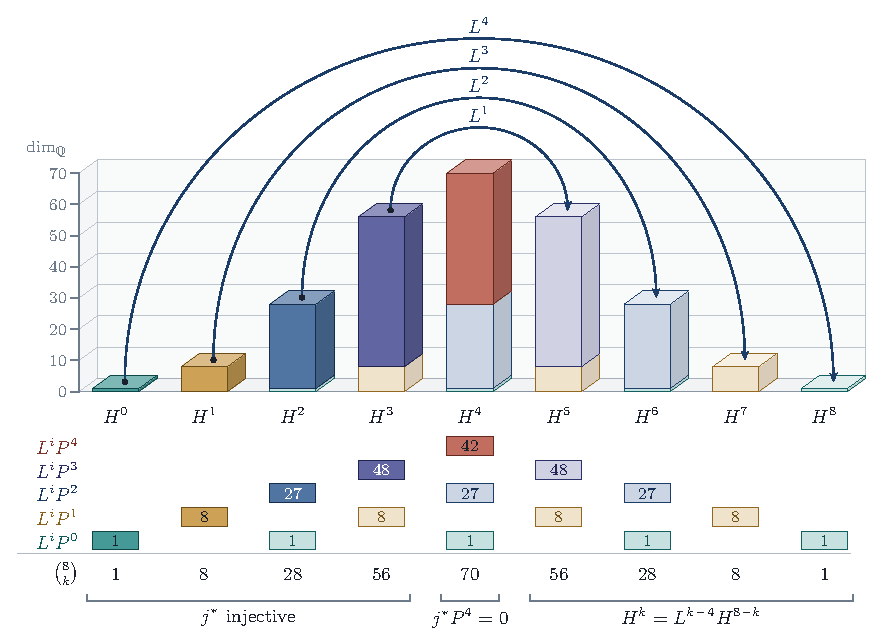
\includegraphics[width=\textwidth]{fig_ladder}
\caption{The Betti numbers $\binom{8}{k}$ of an abelian fourfold, drawn as
prisms and divided according to the Lefschetz decomposition
$H^{k}=\bigoplus_{i}L^{i}P^{k-2i}$: the primitive part $P^{k}$ is drawn dark,
and each image $L^{i}P^{k-2i}$ is drawn light in the colour of $P^{k-2i}$. The
arcs are the hard Lefschetz isomorphisms $L^{4-k}\colon H^{k}\to H^{8-k}$.
Below the middle degree the restriction $j^{*}$ to a smooth ample hypersurface
is injective and a class descends, but the return trip $j_{*}j^{*}$ multiplies
by $L$, and recovering the class is the Lefschetz standard conjecture; above
the middle degree a class is carried to the lower half by an arc. The
primitive middle cohomology $P^{4}$, of dimension $70-28=42$, is annihilated
by $j^{*}$ (\Cref{thm:hyperplane}), and neither an arc nor a restriction
reaches it.}
\label{fig:ladder}
\end{figure}

\section{The Kuga--Satake construction}\label{sec:ks}

\Cref{thm:hyperplane} blocks induction on dimension through hyperplane
sections in the primitive middle degree. One classical construction does reach
a middle degree Hodge class without any such induction, and we set it out in
full, both because it shows what a successful route looks like and because
its boundary is numerical and can be located. It is the construction of Kuga
and Satake \cite{KS67}, which builds on Satake's Clifford algebra families and
their Riemann forms \cite{Sat66}. We follow the form given by Deligne
\cite{Del72}, to whom the Hodge-theoretic properties that make it useful are
due, in particular the embedding of \Cref{prop:ksembed}. After building it we
show that \Cref{thm:hyperplane} has no bearing on it. For abelian varieties of
Weil type with Hodge group $\SU(V,H)$ we then determine when it applies to a
piece of $H^{2}$: exactly when $n=1$, where the Weil line consists of divisor
classes and there is nothing to prove, or $n=2$ with trivial discriminant,
where the Weil line lies in $H^{4}$.

\subsection{The construction}

\begin{setupenv}[K3 type]\label{setup:k3type}
Let $T$ be a $\QQ$-vector space of dimension $b$ with a nondegenerate
symmetric form $q$, and let $T$ carry a Hodge structure of weight two,
$T_{\CC}=T^{2,0}\oplus T^{1,1}\oplus T^{0,2}$, polarised by $q$, with
\[
  \dim_{\CC}T^{2,0}=1 .
\]
Such a structure is said to be \emph{of K3 type}. Write $T^{2,0}=\CC\sigma$.
The Hodge--Riemann relations give $q(\sigma,\sigma)=0$ and
$q(\sigma,\bbar{\sigma})>0$, and make $q$ negative definite on the real points
of $T^{1,1}$; so the real plane
$P=\langle\Re\sigma,\Im\sigma\rangle\subset T_{\RR}$ is positive definite and
$q$ has signature $(2,b-2)$ on $T_{\RR}$. Since $q(\Re\sigma,\Im\sigma)=0$
and $q(\Re\sigma)=q(\Im\sigma)$, we may normalise $\sigma$ so that
$e_{1}=\Re\sigma$ and $e_{2}=\Im\sigma$ are orthonormal.
\end{setupenv}

\begin{definition}[Clifford algebra]\label{def:clifford}
$C(T,q)$ is the quotient of the tensor algebra on $T$ by the ideal generated
by $v\otimes v-q(v)$ for $v\in T$. It is $\ZZ/2$-graded, $C=C^{+}\oplus C^{-}$,
by the parity of the word length.
\end{definition}

\begin{lemma}\label{lem:cliffdim}
For an orthogonal basis $f_{1},\dots,f_{b}$ of $T$ the products $f_{S}$ over
subsets $S\subseteq\{1,\dots,b\}$, taken in increasing order, form a basis of
$C(T,q)$. Hence $\dim_{\QQ}C=2^{b}$ and $\dim_{\QQ}C^{\pm}=2^{b-1}$, and
$C^{-}\cdot C^{+}\cdot C^{-}\subseteq C^{+}$.
\end{lemma}

\begin{proof}
The relations $f_{i}^{2}=q(f_{i})$ and $f_{i}f_{j}=-f_{j}f_{i}$ for $i\ne j$,
the latter obtained by expanding $(f_{i}+f_{j})^{2}=q(f_{i})+q(f_{j})$, let one
rewrite any word in the $f_{i}$ as a scalar times an increasing product, so the
$f_{S}$ span; they are independent by the standard filtration argument
comparing $C$ with $\bigwedge^{*}T$. The dimension counts are
$\sum_{k}\binom{b}{k}=2^{b}$ and
$\sum_{k\ \mathrm{even}}\binom{b}{k}=2^{b-1}$. The last inclusion holds
because the grading is multiplicative and odd plus even plus odd is even.
\end{proof}

\begin{lemma}[The complex structure]\label{lem:cliffJ}
With $e_{1},e_{2}$ as in \Cref{setup:k3type}, put $J=e_{1}e_{2}\in C^{+}\otimes_{\QQ}\RR$.
Then $J^{2}=-1$, and left multiplication by $J$ is an $\RR$-linear operator on
$C^{+}\otimes_{\QQ}\RR$ whose square is $-\id$.
\end{lemma}

\begin{proof}
$J^{2}=e_{1}e_{2}e_{1}e_{2}=-e_{1}e_{1}e_{2}e_{2}=-q(e_{1})q(e_{2})=-1$,
since the orthogonal vectors $e_{1}$ and $e_{2}$ anticommute and
$e_{i}^{2}=q(e_{i})=1$.
Left multiplication by an element of $C^{+}$ preserves $C^{+}$, and the square
of left multiplication by $J$ is left multiplication by $J^{2}=-1$.
\end{proof}

\Cref{fig:ks} draws the positive plane $P$, the null cone of $q$ and the
period domain in the smallest case $b=3$.

\begin{definition}[Kuga--Satake variety]\label{def:ksvariety}
Fix a lattice $C^{+}_{\ZZ}\subset C^{+}$ stable under multiplication. The
complex torus
\[
  \mathrm{KS}(T)=\bigl(C^{+}\otimes_{\QQ}\RR,\,J\bigr)\big/\,C^{+}_{\ZZ}
\]
has dimension $\tfrac12\dim_{\QQ}C^{+}=2^{b-2}$. Satake's construction of a
Riemann form on $C^{+}$ compatible with $J$ \cite{Sat66} makes it an abelian
variety, and by construction
\[
  H^{1}\bigl(\mathrm{KS}(T),\QQ\bigr)=C^{+}(T)
\]
as a Hodge structure of weight one, the Hodge decomposition being the
eigenspace decomposition of left multiplication by $J$.
\end{definition}

\begin{example}\label{ex:ksdims}
For a projective K3 surface, $T$ is the transcendental lattice inside
$H^{2}(X,\QQ)$; taking all of $H^{2}$ with $b=22$ gives
$\dim\mathrm{KS}=2^{20}=1{,}048{,}576$. At the other end, $b=3$ gives
$\dim\mathrm{KS}=2$, an abelian surface, and $b=6$ gives
$\dim\mathrm{KS}=16$; these are the two cases that occur below, for $n=1$ and
for $n=2$.
\end{example}

\subsection{The transport of Hodge classes}

\begin{proposition}[The embedding]\label{prop:ksembed}
Fix $v_{0}\in T$ with $q(v_{0})\ne0$. The map
\[
  \Psi\colon T\longrightarrow\End_{\QQ}\bigl(C^{+}\bigr),
  \qquad
  \Psi(v)(x)=v\,x\,v_{0},
\]
is injective and is a morphism of Hodge structures
$T(1)\to\End\bigl(H^{1}(\mathrm{KS}(T),\QQ)\bigr)$, both sides having weight
zero. Consequently a Hodge class in $T$, that is a rational class of type
$(1,1)$, is carried to a Hodge class of type $(0,0)$ in
$\End(H^{1}(\mathrm{KS}(T),\QQ))$, that is to an element of
$\End^{0}(\mathrm{KS}(T))$.
\end{proposition}

\begin{proof}
The map lands in $\End(C^{+})$ by the last part of \Cref{lem:cliffdim}, since
$v,v_{0}\in T\subset C^{-}$. It is injective because $\Psi(v)(1)=v\,v_{0}$
and $v_{0}$ is invertible in $C(T,q)$, with $v_{0}^{-1}=v_{0}/q(v_{0})$, so
$\Psi(v)=0$ forces $v=0$. That it respects the Hodge structures is
Deligne's computation \cite[\S4]{Del72}: the Hodge structure on
$\End(C^{+})$ is induced by $J$ acting on both sides, and $\Psi$ intertwines
the weight-two structure on $T$, twisted once, with it. The last sentence
follows from the definition of a morphism of Hodge structures and the
Lefschetz theorem on $(1,1)$ classes, in the form which says that for an
abelian variety $B$ a Hodge class of type $(0,0)$ in $\End(H^{1}(B,\QQ))$ is
an element of $\End^{0}(B)$.
\end{proof}

\begin{remark}[Algebraicity of the transport]%
\label{rem:kstransport}
An element of $\End^{0}(\mathrm{KS}(T))$ is a rational multiple of an
endomorphism, whose graph is an algebraic cycle on
$\mathrm{KS}(T)\times\mathrm{KS}(T)$, so the image of a Hodge class under
$\Psi$ is algebraic. Carrying that conclusion back to the variety $X$ from
which $T$ came requires the correspondence $\Psi$ itself to be induced by an
algebraic cycle on $X\times\mathrm{KS}(T)\times\mathrm{KS}(T)$. What is
proved in general is that $\Psi$ is absolute Hodge, by
Deligne's theorem for abelian varieties together with the analysis of the
Kuga--Satake correspondence, and that it is motivated in Andr\'e's sense
\cite{And96}; van Geemen \cite{vG00} surveys the cases in which algebraicity
has been established. The Kuga--Satake construction therefore converts the
Hodge conjecture for $T$ into the algebraicity of one specific
correspondence.
\end{remark}

\subsection{Independence from the hyperplane obstruction}

\begin{proposition}\label{prop:ksnotrestriction}
\Cref{thm:hyperplane,thm:returntrip} do not constrain the Kuga--Satake route.
\end{proposition}

\begin{proof}
Both theorems are statements about the pair of maps $j^{*}$ and $j_{*}$
attached to the inclusion $j\colon Y\hookrightarrow X$ of a smooth member of an
ample linear system, and both proofs use two properties of that pair which a
general correspondence does not have: the Lefschetz hyperplane theorem, which
makes $j^{*}$ an isomorphism in degrees at most $d-2$ and, through
\Cref{lem:gysinrestrict}, forces the vanishing of \Cref{thm:hyperplane} in
the primitive middle degree; and the identity $j_{*}j^{*}=\,\cdot\cup L$ of
\Cref{lem:gysinrestrict}, which makes the return trip multiply by the
polarisation instead of recovering the class. The Kuga--Satake
correspondence is a cohomology class on a triple product of varieties of
unrelated dimensions, $\dim\mathrm{KS}(T)=2^{b-2}$ against $\dim X$, and it has
neither property; in particular the composite of $\Psi$ with its transpose is
a nonzero multiple of the identity of $T$, not a power of a polarisation of
$X$. So
neither of the two properties on which \Cref{thm:hyperplane} rests holds for
$\Psi$.
\end{proof}

\Cref{prop:ksnotrestriction} shows what an escape from \Cref{thm:hyperplane}
must look like: a correspondence whose composite with its transpose is not the
Lefschetz operator. \Cref{sec:escape} makes the analogous identification for
\Cref{thm:divisor,thm:character}.

\subsection{Abelian varieties of Weil type}

The limitation of the Kuga--Satake construction is the hypothesis
$\dim T^{2,0}=1$. For abelian varieties of Weil type the rational sub-Hodge
structures of $H^{2}$, and hence the possible values of $\dim T^{2,0}$, can be
listed completely.

\begin{proposition}[The pieces of \texorpdfstring{$H^{2}$}{H2}]\label{prop:h2pieces}
Let $(A,\iota,\eta)$ be of $(K,-1,n)$-Weil type. In the character grading of
\Cref{prop:grading},
\begin{equation}\label{eq:h2split}
  H^{2}(A,\CC)
  =\textstyle\bigwedge^{2}V_{+}\;\oplus\;\bigl(V_{+}\otimes V_{-}\bigr)
   \;\oplus\;\bigwedge^{2}V_{-},
\end{equation}
the middle summand is the isotypic component of the norm character and is
defined over $\QQ$, and the outer two are interchanged by conjugation so their
sum is defined over $\QQ$. The Hodge numbers are
\[
  \bigl(h^{2,0},h^{1,1},h^{0,2}\bigr)=
  \begin{cases}
    \bigl(\tbinom{n}{2},\,n^{2},\,\tbinom{n}{2}\bigr)
      & \text{on }\bigwedge^{2}V_{\pm},\\[4pt]
    \bigl(n^{2},\,2n^{2},\,n^{2}\bigr)
      & \text{on }V_{+}\otimes V_{-},
  \end{cases}
\]
and the total is $2\tbinom{2n}{2}+4n^{2}=\tbinom{4n}{2}=\dim H^{2}(A,\QQ)$.
\end{proposition}

\begin{proof}
The splitting is \eqref{eq:grading} at $k=2$. The characters are
$\tau^{2}$, $\tau\bbar{\tau}=\Nm(\tau)$ and $\bbar{\tau}^{2}$, so the middle
summand is the norm-isotypic component, and it is self-conjugate, hence defined
over $\QQ$; the outer two are exchanged. For the Hodge numbers use
\eqref{eq:bisplit} and \Cref{lem:balanced}: $V_{\pm}^{1,0}$ and
$V_{\pm}^{0,1}$ have dimension $n$ each, so
$(\bigwedge^{2}V_{+})^{2,0}=\bigwedge^{2}V^{1,0}_{+}$ has dimension
$\binom{n}{2}$ and $(\bigwedge^{2}V_{+})^{1,1}=V^{1,0}_{+}\otimes V^{0,1}_{+}$
has dimension $n^{2}$, while
$(V_{+}\otimes V_{-})^{2,0}=V^{1,0}_{+}\otimes V^{1,0}_{-}$ has dimension
$n^{2}$ and the $(1,1)$ part has dimension $2n^{2}$. The total is
$2(2\binom{n}{2}+n^{2})+4n^{2}=2(2n^{2}-n)+4n^{2}=8n^{2}-2n=\binom{4n}{2}$.
\end{proof}

\begin{proposition}[Sub-Hodge structures of K3 type]%
\label{prop:normpart}
Let $(A,\iota,\eta)$ be of $(K,-1,n)$-Weil type with $\Hg(A)=\SU(V,H)$. Then
$H^{2}(A,\QQ)$ is the direct sum of the three rational sub-Hodge structures
\[
  \QQ\,\eta,
  \qquad
  \bigl(V_{+}\otimes V_{-}\bigr)_{\QQ}\ominus\QQ\eta,
  \qquad
  R=\Bigl(\textstyle\bigwedge^{2}V_{+}\oplus\bigwedge^{2}V_{-}\Bigr)_{\QQ},
\]
with $h^{2,0}$ equal to $0$, $n^{2}$ and $n(n-1)$ respectively. The first two
are irreducible, and so is $R$ when $n\ge3$. When $n=2$, the structure $R$ is
irreducible if the discriminant of $(A,\iota,\eta)$ in the sense of
\Cref{def:disc} is nontrivial, and it is the direct sum of two isomorphic
sub-Hodge structures of K3 type, each of dimension six, if the discriminant
is trivial. Consequently $H^{2}(A,\QQ)$ contains a rational sub-Hodge
structure of K3 type if and only if either $n=1$, or $n=2$ and the
discriminant is trivial.
\end{proposition}

\begin{proof}
A rational sub-Hodge structure $W\subseteq H^{2}(A,\QQ)$ is stable under
$\Hg(A)$: the orthogonal projector onto $W$ for the polarisation is a Hodge
class in $\End(H^{2})$, hence is fixed by $\Hg(A)$, hence $W$ is a
$\Hg(A)$-submodule. Conversely a $\Hg(A)$-submodule is a sub-Hodge structure,
because the Hodge decomposition is the eigenspace decomposition of an element
of $\Hg(A)(\RR)$. So the rational sub-Hodge structures are the
$\QQ$-subrepresentations of $\SU(V,H)$. For the same reason the Hodge numbers
of a sub-Hodge structure depend only on its complexification as a
representation of $\Hg(A)_{\CC}$.

After complexification $\SU(V,H)$ becomes $\SL(V_{+})$, acting on $V_{+}$
tautologically and on $V_{-}\cong V_{+}^{\vee}$ dually. In \eqref{eq:h2split}
the outer summands $\bigwedge^{2}V_{+}$ and
$\bigwedge^{2}V_{-}\cong\bigwedge^{2}V_{+}^{\vee}$ are irreducible, and the
middle summand is $V_{+}\otimes V_{+}^{\vee}=\End(V_{+})
=\mathfrak{sl}(V_{+})\oplus\CC$, the sum of the adjoint representation and the
trivial one. Conjugation fixes the two pieces of the middle summand and
exchanges the outer two, so the three listed subspaces are rational sub-Hodge
structures, and the first two, having irreducible complexifications, are
irreducible. The trivial summand is spanned by $\eta$ by \Cref{lem:NSchar},
and has $h^{2,0}=0$ since $\eta$ is of type $(1,1)$. The adjoint summand has
$h^{2,0}=n^{2}$, since removing the one-dimensional trivial piece from
$V_{+}\otimes V_{-}$ removes a $(1,1)$ class only. The structure $R$ has
$h^{2,0}=2\binom{n}{2}=n(n-1)$ by \Cref{prop:h2pieces}.

The complexification of a rational subrepresentation of $R$ is a
subrepresentation of $\bigwedge^{2}V_{+}\oplus\bigwedge^{2}V_{-}$ stable under
conjugation. For $n\ge3$ the two summands are not isomorphic, because
$\bigwedge^{2}V_{+}^{\vee}\cong\bigwedge^{2n-2}V_{+}$ and $2n-2\ne2$. The
subrepresentations are then $0$, the two summands and the whole; conjugation
exchanges the summands, so only $0$ and the whole are stable under it, and
$R$ is irreducible.
For $n=1$ both summands are the trivial representation, and $R$ is the plane
of Hodge classes $\HW(A)\subset H^{2}(A,\QQ)$.

Let $n=2$. Then $\bigwedge^{2}V_{+}^{\vee}\cong\bigwedge^{2}V_{+}\otimes
(\bigwedge^{4}V_{+})^{\vee}\cong\bigwedge^{2}V_{+}$ as representations of
$\SL(V_{+})$, so $\End_{\Hg(A)}(R)\otimes\CC\cong M_{2}(\CC)$ and
$\End_{\Hg(A)}(R)$ is a quaternion algebra over $\QQ$. To identify it, put
$V=H^{1}(A,\QQ)$, a $K$-vector space of dimension four by \Cref{lem:Kspace}.
The natural map $\bigwedge^{2}_{\QQ}V\to\bigwedge^{2}_{K}V$ is
$\SU(V,H)$-equivariant, and its kernel has complexification
$V_{+}\otimes V_{-}$, so it restricts to an isomorphism of $R$ onto
$\bigwedge^{2}_{K}V$; in particular $K\subseteq\End_{\Hg(A)}(R)$. The wedge
product $B\colon\bigwedge^{2}_{K}V\times\bigwedge^{2}_{K}V\to
\bigwedge^{4}_{K}V\cong K$ is a symmetric $K$-bilinear form, invariant under
$\SU(V,H)$ because $\SU(V,H)$ acts trivially on $\bigwedge^{4}_{K}V$. Let
$H_{2}$ be the hermitian form induced by $H$ on $\bigwedge^{2}_{K}V$, and let
$\varphi$ be the $K$-antilinear map defined by
$B(x,y)=H_{2}\bigl(y,\varphi(x)\bigr)$. Then $\varphi$ commutes with
$\SU(V,H)$, so $\varphi^{2}$ is a $K$-linear endomorphism commuting with
$\SU(V,H)$; it is a scalar by Schur's lemma, and a rational one because it
commutes with $\varphi$. Choose a $K$-basis $e_{1},\dots,e_{4}$ of $V$
orthogonal for $H$, with $H(e_{i},e_{i})=h_{i}\in\QQ^{\times}$, and identify
$\bigwedge^{4}_{K}V$ with $K$ through $e_{1}\wedge e_{2}\wedge e_{3}\wedge
e_{4}$. Then $\varphi(e_{1}\wedge e_{2})=(h_{3}h_{4})^{-1}e_{3}\wedge e_{4}$
and $\varphi(e_{3}\wedge e_{4})=(h_{1}h_{2})^{-1}e_{1}\wedge e_{2}$, so
$\varphi^{2}=(\det H)^{-1}$. Hence $\End_{\Hg(A)}(R)=K\oplus K\varphi$ is the
quaternion algebra $(-d,\det H)_{\QQ}$. It is split if and only if
$\det H\in\Nm_{K/\QQ}(\Kx)$, that is, since $(-1)^{2}\det H=\det H$, if and
only if the discriminant is trivial. If it is not split it is a division
algebra, and $R$ is irreducible. If it is split, $R=R_{1}\oplus R_{2}$ with
$R_{1}\cong R_{2}$ of dimension six, and the complexification of each $R_{i}$
is isomorphic to $\bigwedge^{2}V_{+}$ as a representation of $\SL(V_{+})$, so
by \Cref{prop:h2pieces} each $R_{i}$ has Hodge numbers $(1,4,1)$. Each $R_{i}$
lies in the primitive part of $H^{2}(A,\QQ)$, which is the $\Hg(A)$-stable
complement of $\QQ\eta$, and is polarised by the restriction of the
Hodge--Riemann form; so $R_{i}$ is of K3 type.

Finally, a rational sub-Hodge structure of $H^{2}(A,\QQ)$ is a direct sum of
irreducible ones, each isomorphic to $\QQ\eta$, to the adjoint structure, to
$R$, or, for $n=2$ and trivial discriminant, to $R_{1}$; and $h^{2,0}$ is
additive. A structure of K3 type has $h^{2,0}=1$. For $n=1$ the adjoint
structure has $h^{2,0}=1$. For $n\ge3$ the nonzero values $n^{2}$ and
$n(n-1)$ both exceed $1$. For $n=2$ the values are $0$, $4$, and $2$ for $R$
or $1$ for $R_{1}$, so a structure of K3 type exists if and only if the
discriminant is trivial.
\end{proof}

\begin{corollary}[Where the construction applies]\label{cor:ksboundary}
Let $(A,\iota,\eta)$ be of $(K,-1,n)$-Weil type with $\Hg(A)=\SU(V,H)$. The
Kuga--Satake construction applies to a rational sub-Hodge structure of
$H^{2}(A,\QQ)$ if and only if either $n=1$, or $n=2$ and the discriminant is
trivial. For $n=1$ the Weil line lies in $H^{2}(A,\QQ)$ and consists of
divisor classes, hence of algebraic classes by the Lefschetz theorem on
$(1,1)$ classes, so nothing needs transporting. For $n=2$ the Weil line lies
in $H^{4}(A,\QQ)$, outside the structures to which the construction applies.
\end{corollary}

\begin{proof}
The first clause is \Cref{prop:normpart} with \Cref{setup:k3type}. For $n=1$
we have $2n=2$, so $\HW(A)\subseteq H^{2}(A,\QQ)\cap H^{1,1}(A)$, which is
$\NS(A)\otimes\QQ$ by the Lefschetz theorem on $(1,1)$ classes. For $n=2$ the
Weil line lies in degree $2n=4$.
\end{proof}

\begin{remark}[Higher weight]\label{rem:nohigherks}
For $n\ge2$ the Weil line sits in $H^{2n}(A,\QQ)$ with $2n\ge4$, and the
Clifford construction has no known counterpart in weight greater than two. It
turns a quadratic form into an algebra; the polarisation of a Hodge structure
of weight $w$ is symmetric only when $w$ is even, and even then there is no
reason for its Clifford algebra to carry the right complex structure. One
can instead apply the construction to a sub-Hodge structure of $H^{2}$ and
try to recover the degree $2n$ class from the resulting abelian variety.
\Cref{prop:normpart} rules this out for $n\ge3$, and for $n=2$ at nontrivial
discriminant. At $n=2$ and trivial discriminant the two structures of K3 type
exist, but the Hodge conjecture for abelian fourfolds of Weil type is in any
case a theorem of Markman \cite{Mar25a,Mar25b}, proved at trivial
discriminant also by Floccari and Fu \cite{FF26}. What remains conceivable for
$n\ge3$ is a construction of Kuga--Satake shape for the weight $2n$ structure
directly, producing an auxiliary variety on which the Weil line becomes a
divisor class or an endomorphism. None is known, and \Cref{thm:character} does
not obstruct one: such a construction is a correspondence and need not
produce a $\Kx$-eigenclass. This is the gap of \Cref{rem:nonequivariant},
seen from the other side.
\end{remark}

\begin{figure}[htbp]
\centering
  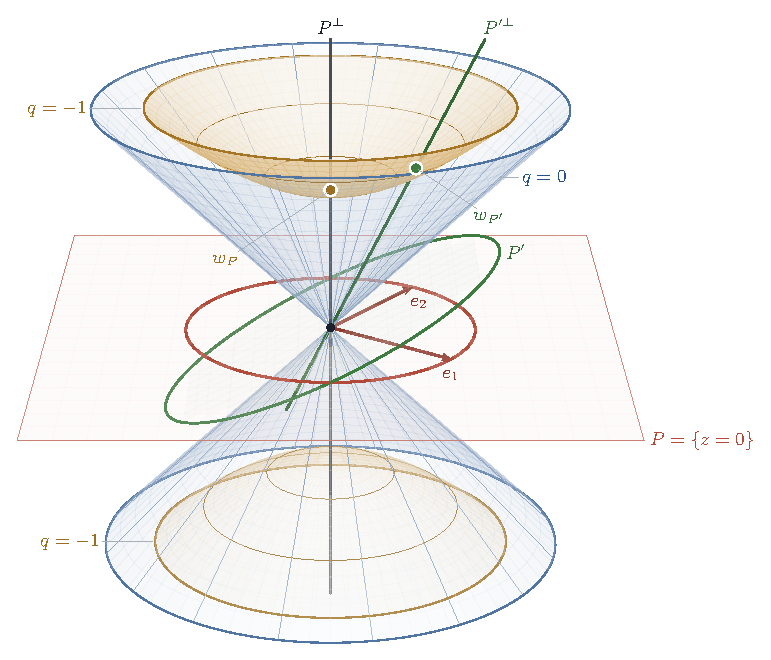
\includegraphics[width=0.88\textwidth]{fig_lightcone}
\caption{The geometry from which the Kuga--Satake construction starts, in the
smallest case $b=3$. The quadratic form is $q=x^{2}+y^{2}-z^{2}$, of
signature $(2,1)$, with its null cone $q=0$; the horizontal plane
$P=\{z=0\}$ is positive definite and meets the cone only at the origin. The
construction needs such a plane, and \Cref{setup:k3type} supplies one:
$P=\langle\Re\sigma,\Im\sigma\rangle$ for the period $\sigma$ spanning
$T^{2,0}$. An orthonormal basis $e_{1},e_{2}$ of $P$ gives $J=e_{1}e_{2}$ with
$J^{2}=-1$ by \Cref{lem:cliffJ}, and $J$ is the complex structure of
$\mathrm{KS}(T)$. A positive definite plane $P$ is determined by the negative
line $P^{\perp}$, which meets the upper sheet of the hyperboloid $q=-1$ in one
point $w_{P}$; that sheet is the period domain, and a second plane $P'$ with
its point $w_{P'}$ is drawn for comparison. The hypothesis behind all of this
is $\dim T^{2,0}=1$, and by \Cref{prop:normpart} an abelian variety of Weil
type with Hodge group $\SU(V,H)$ supplies it in $H^{2}$ only when $n=1$, or
$n=2$ at trivial discriminant.}
\label{fig:ks}
\end{figure}

\section{Reduction to the middle degree}\label{sec:reduction}

The two preceding sections dealt with restriction to hypersurfaces and with
the one classical correspondence that avoids it. Here we combine the first of
them with the Lefschetz decomposition to locate the difficulty of the Hodge
conjecture in general. The result, \Cref{thm:equivalence}, is an equivalence
in which neither side is easier than the other. Its use is to isolate the
primitive classes of middle degree as the one place where a new method is
needed, and by \Cref{thm:hyperplane} restriction to hyperplane sections sees
nothing there.

\subsection{Reduction to primitive classes}

\begin{proposition}[Lefschetz decomposition of Hodge classes]%
\label{prop:lefschetzdecomp}
Let $X$ be smooth projective of dimension $d$ with ample class $L$. Every
$\alpha\in\Hdg^{p}(X)$ can be written
\[
  \alpha=\sum_{r\ge\max(0,\,2p-d)}L^{r}\beta_{r},
  \qquad
  \beta_{r}\in\Hdg^{p-r}(X)\cap H^{2p-2r}_{\mathrm{prim}}(X,\QQ),
\]
and the $\beta_{r}$ are uniquely determined. Consequently the Hodge conjecture
holds for $X$ if and only if every primitive rational Hodge class on $X$ is
algebraic.
\end{proposition}

\begin{proof}
The Lefschetz decomposition
$H^{k}(X,\QQ)=\bigoplus_{r}L^{r}H^{k-2r}_{\mathrm{prim}}(X,\QQ)$ is a
decomposition of rational Hodge structures, because $L$ is a rational class
of type $(1,1)$ and the primitive parts are kernels of morphisms of Hodge
structures. The rationality of $L$ is essential here: for a K\"ahler class
that is not a real multiple of a rational one the primitive subspaces are in
general not rational, and a rational Hodge class need not decompose into
rational primitive pieces. A Hodge class $\alpha$ therefore has Hodge classes
$L^{r}\beta_{r}$ as its components. By hard Lefschetz, $L^{r}$ is injective
on $H^{2p-2r}_{\mathrm{prim}}(X,\QQ)$ for $r\ge\max(0,2p-d)$, and it is a
morphism of Hodge structures of bidegree $(r,r)$, so each $\beta_{r}$ is
uniquely determined and is itself a Hodge class. For the last statement, if
each primitive $\beta_{r}$ is algebraic then so is $L^{r}\beta_{r}$, since $L$
is algebraic and algebraic classes form a subring, and hence so is $\alpha$;
the converse holds because primitive Hodge classes are Hodge classes.
\end{proof}

\subsection{The equivalence}

\begin{theorem}\label{thm:equivalence}
The following are equivalent.
\begin{enumerate}[label=\textup{(\roman*)}]
\item The Hodge conjecture holds for every smooth complex projective variety.
\item The Lefschetz standard conjecture $B(X)$ holds for every smooth complex
  projective variety $X$, and every primitive rational Hodge class of middle
  degree on every smooth complex projective variety of even dimension is
  algebraic.
\end{enumerate}
\end{theorem}

\begin{proof}
(i) implies (ii). The second half of (ii) is a special case of (i). For
$B(X)$, note that $\Lambda$ is a morphism of Hodge structures of bidegree
$(-1,-1)$, hence is given by a Hodge class on $X\times X$ through the
standard correspondence between morphisms of Hodge structures and Hodge
classes on the product, and (i) applied to $X\times X$ makes that class
algebraic. This is Kleiman's argument \cite[\S2]{Kle68}.

(ii) implies (i). We argue by induction on $d=\dim X$. For $d\le1$ the Hodge
conjecture is classical. Let $d\ge2$ and assume the conjecture for all smooth
projective varieties of dimension less than $d$. By Bertini there is a smooth
hypersurface $j\colon Y\hookrightarrow X$ in $|mH|$ for an ample $H$ and
$m\gg0$; put $L=c_{1}(\cO_{X}(Y))$, and take primitivity and the operator
$\Lambda$ with respect to this $L$, which is harmless because $B(X)$ does not
depend on the choice of ample class \cite{Kle68,Kle94}. By
\Cref{prop:lefschetzdecomp} it suffices to prove that a primitive Hodge class
$\alpha\in H^{2p}(X,\QQ)$ is algebraic and, by hard Lefschetz, primitive
classes occur only in degrees at most $d$, so $2p\le d$.

If $2p=d$, then $\alpha$ is a primitive Hodge class of middle degree on a
variety of even dimension, so it is algebraic by the second half of (ii).

If $2p<d$, the class $j^{*}\alpha$ is a rational Hodge class on $Y$ because
$j^{*}$ is a morphism of Hodge structures. As $\dim Y=d-1<d$, the inductive
hypothesis makes $j^{*}\alpha$ algebraic, say $j^{*}\alpha=\cl(W)$ with
$W\in\CH^{p}(Y)_{\QQ}$. Then
$\cl(j_{*}W)=j_{*}j^{*}\alpha=L\alpha$ by \Cref{lem:gysinrestrict}, so
$L\alpha$ is algebraic. By $B(X)$ the operator $\Lambda$ carries algebraic
classes to algebraic classes, and by \Cref{lem:LambdaL},
$\alpha=(d-2p)^{-1}\Lambda(L\alpha)$, which is therefore algebraic; the scalar
is defined because $d-2p\ge1$.
\end{proof}

\begin{remark}[The content of the equivalence]\label{rem:notsimpler}
$B(X)$ is itself a consequence of (i), so
\Cref{thm:equivalence} does not reduce the problem to a smaller one; it
locates the difficulty. The induction in the proof that (ii) implies (i) runs
through every degree except the middle one, where it rests entirely on the
hypothesis. By \Cref{thm:hyperplane}, the step it uses below the middle
degree, restriction to a hypersurface, returns zero on primitive classes of
middle degree, so no refinement of that step extends the induction to that
degree.
\end{remark}

\begin{corollary}[Primitive classes of middle degree]\label{cor:whereidea}
Any proof of the Hodge conjecture must, at some point, produce an algebraic
cycle representing a primitive Hodge class of middle degree on a variety of
even dimension, by a method that does not factor through restriction to
hyperplane sections of that variety.
\end{corollary}

\begin{proof}
By \Cref{thm:equivalence}, the Hodge conjecture includes the algebraicity of
the primitive Hodge classes of middle degree on varieties of even dimension,
and by \Cref{cor:blind} every such class restricts to zero on every smooth
ample hypersurface.
\end{proof}

\begin{remark}[Methods that do not factor through hyperplane sections]%
\label{rem:othermethods}
\Cref{cor:whereidea} does not say that the conjecture is out of reach, and
the settled cases come from known methods outside its scope. The
Kuga--Satake construction (\Cref{sec:ks}) replaces a weight-two Hodge
structure of K3 type by the $H^{1}$ of an abelian variety; the class it
produces is of type $(1,1)$ on a product, hence algebraic by Lefschetz, and it
is not a restriction to a subvariety. Degenerations and limits of Hodge
structures move the variety instead of cutting it. Correspondences from other
varieties, of which the Kuga--Satake construction is one instance and
Markman's construction \cite{Mar25a,Mar25b} another, are also outside the
scope. Arguments through the coniveau filtration, which show that a class
supported on a proper closed subvariety is controlled by that subvariety, are
compatible with everything here: they lower the dimension legitimately,
because the class is supported on the smaller variety, whereas a primitive
class of coniveau zero is supported on no proper closed subvariety.
\end{remark}


\section{Equivariance and Markman's construction}
\label{sec:escape}

We return to abelian varieties of Weil type. By \Cref{thm:character}, a
$\Kx$-eigenclass for the norm character has no component along the Weil line,
and we ask what the contrapositive demands of a construction that does reach
the Weil line. The demand does not concern the size of the object, the ambient
geometry or any dimension count; it concerns the way the object transforms
under $\Kx$. We state it in a concrete form and then show how Markman's
construction meets it.

\subsection{The orbit criterion}

\begin{proposition}[Weil classes generate a plane]\label{prop:orbitplane}
Let $(A,\iota,\eta)$ be of $(K,-1,n)$-Weil type and let $\alpha\in\HW(A)$ be
nonzero. Then
\[
  \mathrm{span}_{\QQ}\bigl\{\iota(\tau)^{*}\alpha\;:\;\tau\in\Kx\bigr\}
  \;=\;\HW(A),
\]
a two-dimensional $\QQ$-vector space, and as a representation of $\Kx$ it is
irreducible over $\QQ$.
\end{proposition}

\begin{proof}
By \Cref{prop:weilline}(i) the space $\HW(A)$ is free of rank one over $K$, and
$\iota(\tau)^{*}$ acts on it as multiplication by the scalar $\tau^{2n}\in K$.
Hence the span in question is $S\cdot\alpha$, where
$S=\mathrm{span}_{\QQ}\{\tau^{2n}:\tau\in\Kx\}\subseteq K$. Taking $\tau=1$
shows $1\in S$. By the argument in the proof of \Cref{lem:charsdiffer} the map
$c(\tau)=\tau/\bbar{\tau}$ has infinite image while $\mu(K)$ is finite, so there
is $\tau_{0}$ with $(\tau_{0}/\bbar{\tau_{0}})^{2n}\ne1$, that is with
$\tau_{0}^{2n}\ne\bbar{\tau_{0}}^{\,2n}$, that is with $\tau_{0}^{2n}\notin\QQ$.
Then $S\supseteq\QQ+\QQ\tau_{0}^{2n}=K$, so $S=K$ and the span is
$K\alpha=\HW(A)$.

For irreducibility, a proper nonzero $\Kx$-stable $\QQ$-subspace would be a
line $\QQ\alpha'$, on which $\Kx$ would act by a $\QQ$-valued character. Since
$\iota(\tau)^{*}\alpha'=\tau^{2n}\alpha'$ and $\HW(A)$ is free over $K$, this forces
$\tau^{2n}\in\QQ$ for all $\tau$, which we have just excluded.
\end{proof}

\begin{corollary}[The orbit criterion]\label{cor:orbitcriterion}
Let $\cE$ be an object of $D^{b}(A)$, or $Z$ a cycle in $\CH^{n}(A)_{\QQ}$,
whose class $\ch_{n}(\cE)$, respectively $\cl(Z)$, is a nonzero Weil class.
Then there is no function $\chi\colon\Kx\to\QQ$ with
\[
  \iota(\tau)^{*}\ch_{n}(\cE)=\chi(\tau)\,\ch_{n}(\cE)
  \qquad\text{for all }\tau\in\Kx .
\]
Equivalently, the $\Kx$-orbit of the class spans a plane and not a line.
\end{corollary}

\begin{proof}
Such a $\chi$ would make $\QQ\cdot\ch_{n}(\cE)$ a $\Kx$-stable line inside
$\HW(A)$, contradicting \Cref{prop:orbitplane}.
\end{proof}

\Cref{cor:orbitcriterion} says in what sense a construction that reaches the
Weil line must break equivariance. Suppose that a construction assigns to the data
$(A,\iota,\eta)$ an object $\cE(A,\iota,\eta)$ naturally, in the sense that
an isomorphism of the data induces an isomorphism of the objects. For
$\tau\ne0$ in the order of $K$ the endomorphism $\iota(\tau)$ is an isogeny of
$A$ commuting with $\iota$ and multiplying $\eta$ by $\Nm(\tau)$, and one
expects naturality to give $\iota(\tau)^{*}\cE\cong\cE$ up to a
normalisation imposed by the change of polarisation, whose effect on
$\ch_{n}$ is multiplication by a rational number $\chi(\tau)$, a power of the
norm. Whenever that is the case, \Cref{cor:orbitcriterion} shows that
$\ch_{n}(\cE)$ is not a nonzero Weil class. A construction that reaches the
Weil line must therefore depend on a choice that $\Gal(K/\QQ)$ moves. The rest
of this section describes such a choice.

\subsection{The two conjugate isotropic subspaces}

The choice that $\Gal(K/\QQ)$ moves is already visible in
\Cref{sec:characters}. The splitting
$V_{\CC}=V_{+}\oplus V_{-}$ of \eqref{eq:Vsplit} is defined over $K$ and not
over $\QQ$, since conjugation interchanges the two summands. Hence
$\bigwedge^{2n}V_{+}$ and $\bigwedge^{2n}V_{-}$ are each defined over $K$,
and only their sum is rational. A class in $\HW(A)$ is of the form
$w+\bbar{w}$ with $w\in\bigwedge^{2n}V_{+}$, and we call $\bigwedge^{2n}V_{+}$
and $\bigwedge^{2n}V_{-}$ the two conjugate halves.

\begin{definition}[Conjugate pair data]\label{def:conjpair}
By \emph{conjugate pair data} for $(A,\iota,\eta)$ we mean a choice of one of
the two summands $V_{\pm}$, equivalently of one of the two embeddings
$K\hookrightarrow\CC$, equivalently of one of the two points of a
$\Gal(K/\QQ)$-orbit of size two attached to the $K$-structure.
\end{definition}

\begin{proposition}[Corestriction produces the plane]\label{prop:corestriction}
Let $w\in\bigwedge^{2n}V_{+}$ be nonzero. Then $w+\bbar{w}$ and
$\sqrt{-d}\,(w-\bbar{w})$ lie in $\HW(A)$ and span it over $\QQ$. In
particular, the rational classes in the Weil line are the
$\Gal(K/\QQ)$-corestrictions of the classes in one conjugate half, and any
construction producing such a class must produce, in effect, a pair of
conjugate inputs and combine them.
\end{proposition}

\begin{proof}
Conjugation interchanges $w$ and $\bbar{w}$ and sends $\sqrt{-d}$ to
$-\sqrt{-d}$, so both elements are fixed by it and are therefore rational.
Both lie in $\bigwedge^{2n}V_{+}\oplus\bigwedge^{2n}V_{-}$ by construction,
hence in $\HW(A)$ by \Cref{def:weilline}. They are linearly independent over
$\QQ$ because $w$ and $\bbar{w}$ are linearly independent over $\CC$: a
relation $q_{1}(w+\bbar{w})+q_{2}\sqrt{-d}\,(w-\bbar{w})=0$ with
$q_{1},q_{2}\in\QQ$ forces $q_{1}+q_{2}\sqrt{-d}=0$, that is $q_{1}=q_{2}=0$.
Since $\HW(A)$ has dimension two by \Cref{prop:weilline}(i), they span it.
\end{proof}

A construction reaching the Weil line therefore has to be, in a suitable
sense, bilinear in the two conjugate halves: it takes one input attached to
$V_{+}$ and one attached to $V_{-}$ and pairs them. A construction fed a
single $K$-invariant input cannot do this, by \Cref{cor:orbitcriterion}.

\subsection{Markman's construction}

Markman's construction \cite{Mar25a,Mar25b} produces Weil classes, and it
meets the criterion in the manner just described. We set out only the
structure relevant here; the details are in \cite{Mar25b}.

The construction does not begin on $A$ or on $\Av$. It begins on an abelian
$n$-fold $X$, that is, on a variety of half the dimension of $A$. Inside
$H^{\mathrm{ev}}(X,\QQ)$ one selects a plane $P$ spanned by Hodge classes, and
one requires that $P$ meet the spinor variety of even pure spinors in two
points. Those two points are conjugate over the imaginary quadratic field $K$;
they correspond to two maximal isotropic subspaces $W_{1}$ and $W_{2}$ that are
interchanged by $\Gal(K/\QQ)$. This is the conjugate pair data of
\Cref{def:conjpair}, realised concretely.

To the two points one attaches \emph{secant sheaves} on $X$, coherent
sheaves whose Chern characters are rational points of $P$. In the worked case
in which $X$ is the Jacobian of a curve of genus three, the secant sheaf is
$\mathcal{I}_{\cup C_{i}}(\Theta)$, the twist by the theta bundle of the ideal
sheaf of a union of translates of the Abel--Jacobi image of the curve. Call the
two sheaves used $\cF_{1}$ and $\cF_{2}$.

The abelian variety of Weil type is then $A=X\times\widehat{X}$, of dimension
$2n$, with its $K$-action and polarisation inherited from $P$. The object that
carries the Weil class is
\begin{equation}\label{eq:markmanobject}
  E=\Phi\bigl(\cF_{1}^{\vee}\boxtimes\cF_{2}\bigr),
\end{equation}
where $\Phi\colon D^{b}(X\times X)\to D^{b}(X\times\widehat{X})$ is Orlov's
derived equivalence. One then shows that the characteristic class $\kappa(E)$
remains of Hodge type under every deformation of $X\times\widehat{X}$ as a
polarised abelian $2n$-fold of Weil type, which is what makes the class
algebraic on the whole family. The conclusion in \cite{Mar25b} is the
algebraicity of the Weil classes for abelian sixfolds of Weil type of trivial
discriminant in the normalisation of \Cref{def:disc} (discriminant $-1$ in
Markman's normalisation), and, through Schoen's product argument
\cite[Proposition~10]{Sch98}, for all abelian fourfolds of Weil type, whence
the Hodge conjecture for abelian fourfolds.

\begin{proposition}[Which hypotheses are escaped]\label{prop:whichescaped}
The object \eqref{eq:markmanobject} satisfies none of the hypotheses of
\Cref{thm:divisor} and does not satisfy the hypothesis of
\Cref{thm:equivsuffices}. Specifically:
\begin{enumerate}[label=\textup{(\roman*)}]
\item \emph{The source is not a projective space.} The input
  $\cF_{1}^{\vee}\boxtimes\cF_{2}$ lives on $X\times X$, an abelian variety.
  The proof of \Cref{thm:divisor} used that $H^{*}(\PP^{N-1},\QQ)$ is generated
  in degree two, so that $\ch$ of any object is a polynomial in the hyperplane
  class. The cohomology of $X\times X$ is not generated in degree two: it
  contains K\"unneth classes of every degree, and $\ch(\cF_{1}^{\vee}\boxtimes\cF_{2})$
  is not confined to any divisor subring.
\item \emph{The transform is not $\Phi_{\cP}$ on $A\times\Av$.} The relevant
  equivalence is between $D^{b}(X\times X)$ and $D^{b}(X\times\widehat{X})$,
  and \Cref{thm:fmtheta}, which computes the transform with Poincar\'e kernel
  on powers of the polarisation of $A$, says nothing about it.
\item \emph{The construction is not $K$-equivariant.} The two tensor factors
  of \eqref{eq:markmanobject} carry the two conjugate points of
  $P\cap(\text{spinor variety})$, one each. Interchanging them is the action of
  the nontrivial element of $\Gal(K/\QQ)$, and it exchanges $E$ with a
  different object. Hence $\ch_{n}(E)$ is not a $\Kx$-eigenclass for the norm,
  and \Cref{cor:orbitcriterion} is satisfied rather than violated.
\end{enumerate}
\end{proposition}

\begin{proof}
Items (i) and (ii) are a comparison of hypotheses and need no argument beyond
reading \eqref{eq:markmanobject}. For (iii), if $\ch_{n}(E)$ were an
eigenclass for the norm, then by \Cref{cor:equivariant} it would have zero
component along the Weil line, whereas Markman shows that this component is
nonzero \cite{Mar25b}.
\end{proof}

The three hypotheses of \Cref{prop:whichescaped} are related. A construction
that takes its input from projective space is normally equivariant for
whatever acts on the input, and an equivariant construction normally returns
a single eigenclass, so the three tend to hold or fail together.

\begin{remark}[Where secant geometry must be placed]\label{rem:secantlesson}
Secant geometry can produce Weil classes: Markman's construction is a secant
construction. The obstructions bear on its placement. Secant geometry placed
on the dual $\Av$ of the $2n$-fold inside an ambient projective space, and
transported by the Poincar\'e kernel, has three defects at once, by
\Cref{prop:whichescaped}: its input lies where the cohomology is generated by
a divisor, it uses the transform to which \Cref{thm:fmtheta} applies, and it
feeds the construction $K$-invariant data, since a secant variety of a
$K$-invariant subvariety is $K$-invariant. Placing the secant geometry on an
abelian $n$-fold removes all three, and it does so because halving the
dimension makes room for the two conjugate inputs.
\end{remark}

\subsection{Beyond the known range}

The algebraicity of the Weil classes is known for $n=2$, for every
discriminant, and for $n=3$ with trivial discriminant; see \cite{Mar25b} and,
for a different route at $n=2$ and trivial discriminant, \cite{FF26}. We state
what a construction of the same shape would have to supply for $n\ge4$.

\begin{question}\label{q:higher}
Fix $n\ge4$ and an imaginary quadratic field $K$. Does there exist an abelian
$n$-fold $X$, a plane $P\subset H^{\mathrm{ev}}(X,\QQ)$ spanned by Hodge
classes meeting the spinor variety in two points conjugate over $K$, secant
sheaves $\cF_{1},\cF_{2}$ on $X$ realising those two points, and a deformation
argument showing that $\kappa\bigl(\Phi(\cF_{1}^{\vee}\boxtimes\cF_{2})\bigr)$
remains of Hodge type across the moduli of polarised abelian $2n$-folds of
Weil type with multiplication by $K$?
\end{question}

Each of the four ingredients is a concrete demand. By
\Cref{cor:orbitcriterion}, any answer must be bilinear in a pair of conjugate
inputs, since that is the only way a rational class can acquire a
$\Kx$-orbit spanning a plane. \Cref{sec:construction} supplies the first three
ingredients explicitly, for every $n\ge2$ and every imaginary quadratic field,
with $X$ an arbitrary polarised abelian $n$-fold. The fourth, the deformation
argument, is isolated in \Cref{rem:deformation}, which says exactly what it
requires.

\begin{figure}[htbp]
\centering
  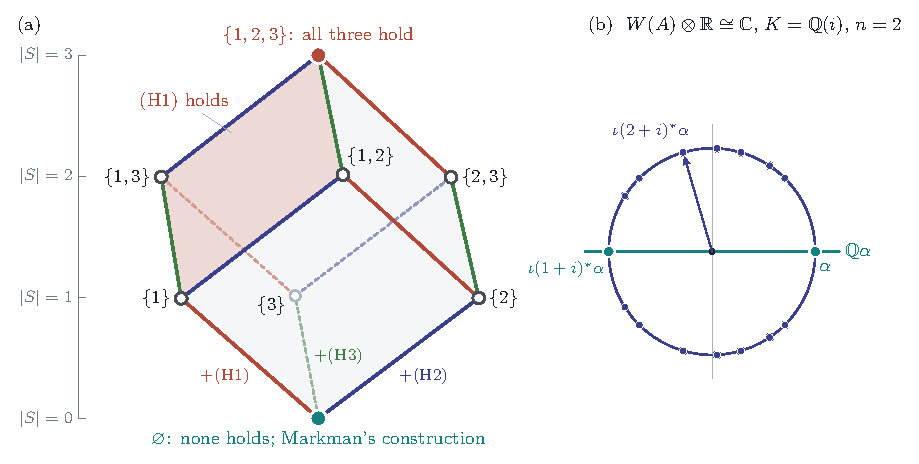
\includegraphics[width=0.97\textwidth]{fig_escape}
\caption{(a) The eight positions a construction can occupy, drawn as the
Boolean lattice of the subsets $S$ of three hypotheses: (H1) the Chern
character of the input lies in the subring generated by divisor classes;
(H2) the output is a $\Kx$-eigenclass; (H3) the output spans a single line
rather than a plane. (H1) and (H2) are the hypotheses negated in (i) and
(iii) of \Cref{prop:whichescaped}, and (H3) is what \Cref{cor:orbitcriterion}
excludes for a nonzero Weil class. At the top vertex all three hold, and both
\Cref{thm:divisor} and \Cref{thm:character} apply; on the shaded face (H1)
holds, and \Cref{thm:divisor} alone already applies. Markman's construction
sits at the bottom vertex, where none of the three holds. (b) The orbit of a
Weil class $\alpha$ under $\Kx$ for $K=\QQ(i)$ and $n=2$, in
$\HW(A)\otimes\RR\cong\CC$ and normalised to the unit circle. Since
$\iota(\tau)^{*}$ acts through $\tau^{4}$, the class $\iota(1+i)^{*}\alpha=-4\alpha$
stays on the line $\QQ\alpha$, while $\iota(2+i)^{*}\alpha$, with
$(2+i)^{4}=-7+24i$, does not; the orbit spans the plane, as
\Cref{prop:orbitplane} asserts.}
\label{fig:escape}
\end{figure}


\part{Base points and the algebraic locus}\label{part:basepoints}
\section{An explicit secant plane in every dimension}\label{sec:construction}

\Cref{q:higher} asks for four things: an abelian $n$-fold $X$, a plane
$P\subset H^{\mathrm{ev}}(X,\QQ)$ of Hodge classes meeting the spinor variety
in two points conjugate over $K$, a pair of secant sheaves realising the
plane, and a deformation argument. This section supplies the first three, for
every $n\ge2$ and every imaginary quadratic field $K$. The first two are
written in closed form (\Cref{thm:explicitweil,thm:plane}). The third is first
reduced to an explicit equation on a Chern character
(\Cref{thm:secantinvariants}) and then solved, in every dimension, by sheaves
of positive rank whose classes are combinations of the powers of a single line
bundle (\Cref{thm:secantexists}). The fourth ingredient is the deformation
argument, and \Cref{rem:deformation} says exactly what it requires.

The framework is Markman's \cite{Mar25a,Mar25b}: the Weil structure on
$X\times\widehat{X}$ obtained by embedding $K$ into
$\End^{0}(X\times\widehat{X})$, the notion of a $K$-secant sheaf, whose Chern
character lies in a plane meeting the spinor variety at two conjugate points,
and the deformation step that completes the argument at $n=3$ are all his.
What we add is the explicit form of the first three ingredients, uniformly in
$n$ and $K$. The closed form rests on two facts: the two conjugate isotropic
subspaces demanded by \Cref{cor:orbitcriterion} are the graphs of multiples of
a single element of the N\'eron--Severi group, and the pure spinor of the graph
of a two-form is the exponential of that form.

\subsection{The Weil structure}

\begin{setupenv}\label{setup:construction}
Let $X$ be a complex abelian variety of dimension $n$ with
$H_{1}(X,\QQ)=U$ of dimension $2n$ and complex structure $J$ on
$U\otimes\RR$. Let $d$ be a squarefree positive integer, $s=\sqrt{-d}$ and
$K=\QQ(s)$. Let $\beta\in\NS(X)\otimes\QQ$ be nondegenerate, regarded as an
alternating form on $U$, so that the Riemann relation $J^{\top}\beta J=\beta$
holds, and write $\phi_{\beta}\colon X\to\widehat{X}$ for the associated
isogeny. Put
\[
  A=X\times\widehat{X},\qquad \dim A=2n,\qquad
  H_{1}(A,\QQ)=U\oplus U^{\vee},
\]
and let
\begin{equation}\label{eq:Mdef}
  M=\begin{pmatrix}0 & -\beta^{-1}\\[2pt] d\,\beta & 0\end{pmatrix}
  \in\End^{0}(A),
\end{equation}
acting on $H_{1}(A,\QQ)=U\oplus U^{\vee}$ by
$(u,\phi)\mapsto(-\beta^{-1}\phi,\;d\,\beta u)$.
\end{setupenv}

\begin{theorem}[An explicit Weil structure]\label{thm:explicitweil}
In \Cref{setup:construction}:
\begin{enumerate}[label=\textup{(\roman*)}]
\item $M^{2}=-d$, so $\iota(s)=M$ defines an embedding
  $\iota\colon K\hookrightarrow\End^{0}(A)$;
\item $M$ commutes with the complex structure of $A$, and for an
  alternating form $\beta$ on $U$ this is equivalent to the Riemann relation,
  that is to $\beta\in\NS(X)\otimes\QQ$;
\item $M$ acts on $H^{1,0}(A)$ with eigenvalues $s$ and $-s$, each of
  multiplicity $n$, so $(A,\iota,\eta)$ is of $(K,-1,n)$-Weil type for a
  suitable polarisation $\eta$;
\item the eigenspaces $W_{\pm}\subset H_{1}(A,\CC)$ of $M$ for $\pm s$ are
  maximal isotropic for the canonical pairing on $U\oplus U^{\vee}$, are
  interchanged by complex conjugation, and are the graphs of the two-forms
  $\mp s\beta$.
\end{enumerate}
\end{theorem}

\begin{proof}
(i) Block multiplication gives
$M^{2}=\mathrm{diag}(-\beta^{-1}\,d\beta,\;-d\beta\,\beta^{-1})=-d\cdot\mathrm{id}$.

(ii) The complex structure of $A=X\times\widehat{X}$ is
$J_{A}=\mathrm{diag}(J,-J^{\top})$. The relation $MJ_{A}=J_{A}M$ amounts to
the two identities $d\beta J=-dJ^{\top}\beta$ and
$-\beta^{-1}(-J^{\top})=J(-\beta^{-1})$, and each is equivalent to
$\beta J=-J^{\top}\beta$. This is the Riemann relation: from
$J^{\top}\beta J=\beta$ and $J^{2}=-1$ one gets
$J^{\top}\beta=\beta J^{-1}=-\beta J$, as required. Conversely
$\beta J=-J^{\top}\beta$ gives $J^{\top}\beta J=-\beta J J=\beta$.

(iii) $M$ is block anti-diagonal and $H^{1,0}(A)=H^{1,0}(X)\oplus
H^{1,0}(\widehat{X})$ with both summands of dimension $n$, and $M$ exchanges
them. If $M(x,y)=\lambda(x,y)$ then $-\beta^{-1}y=\lambda x$ and
$d\beta x=\lambda y$, so $y=d\beta x/\lambda$ and, substituting,
$-dx/\lambda=\lambda x$, that is $\lambda^{2}=-d$. For each of
the two values of $\lambda$ the assignment $x\mapsto(x,d\beta x/\lambda)$ is an
isomorphism from $H^{1,0}(X)$ onto the $\lambda$-eigenspace, which is
therefore of dimension $n$. That is the balanced signature of
\Cref{def:weiltype}(ii). For (iii) of that definition, let $\eta_{0}$ be any
polarisation of $A$ and put
$\eta(x,y)=\eta_{0}(x,y)+d^{-1}\eta_{0}(Mx,My)$. A positive integer multiple
$mM$ of $M$ is an isogeny, so the second term is the positive multiple
$(dm^{2})^{-1}(mM)^{*}\eta_{0}$ of a polarisation, and $\eta$ is a
polarisation. Since $M^{2}=-d$,
$\eta(Mx,My)=\eta_{0}(Mx,My)+d\,\eta_{0}(x,y)=d\,\eta(x,y)$, and as
$M^{-1}=-M/d$ this gives $\eta(Mx,y)=-\eta(x,My)$: the Rosati involution of
$\eta$ sends $M$ to $-M$, that is $\iota(\tau)^{\dagger}=\iota(\bbar{\tau})$.
When $\beta$ is a polarisation an explicit choice of $\eta$ is recorded in
\Cref{prop:splitgeom}(i).

(iv) The same computation identifies $W_{\lambda}=\{(x,d\beta x/\lambda)\}$,
the graph of the form $d\beta/\lambda$, and
$d\beta/\lambda=d\beta/(\pm s)=\mp s\beta$ since $d/s=-s$. The canonical
pairing on $U\oplus U^{\vee}$ is
$\langle(x,\xi),(x',\xi')\rangle=\xi'(x)+\xi(x')$, and on the graph it gives
$d\beta(x',x)/\lambda+d\beta(x,x')/\lambda=0$ because $\beta$ is alternating; so
$W_{\lambda}$ is isotropic, and it has dimension $2n$, half of
$\dim(U\oplus U^{\vee})=4n$, hence is maximal. Conjugation sends $s$ to $-s$
and so interchanges the two.
\end{proof}

The placement of the factor $d$ in \eqref{eq:Mdef} is a convention, fixed once
and for all. The endomorphism $\begin{psmallmatrix}0&-d\beta^{-1}\\
\beta&0\end{psmallmatrix}$ also squares to $-d$, commutes with the complex
structure and defines a Weil structure on the same $A$, but it is a different
embedding of $K$: its eigenspaces are the graphs of $\mp s\beta/d$ rather
than of $\mp s\beta$, its polarisation is $\beta+d\widehat\beta$ rather than
$d\beta+\widehat\beta$, and the class in
$\bigwedge^{2}V_{+}\oplus\bigwedge^{2}V_{-}$ it produces is
$\beta-d\widehat\beta$ rather than $\gamma=d\beta-\widehat\beta$. The
convention of \eqref{eq:Mdef} is the one whose action on cohomology is
$x\mapsto-Bx$, $\xi\mapsto dB^{-1}\xi$ in the proof of
\Cref{thm:splitclosed}, and every formula below refers to it. For $d=1$ the
two conventions coincide.

\begin{remark}\label{rem:abundant}
\Cref{thm:explicitweil} says that abelian $2n$-folds of Weil type of the split
form $X\times\widehat{X}$ exist for every $n$, every imaginary quadratic $K$
and every polarised abelian $n$-fold $X$, and that the Weil structure is
written down by one element of $\NS(X)$. These are not general members of the
moduli of Weil type. The Weil classes on them are of interest because
Markman's deformation argument, where it can be carried out, propagates
algebraicity from them to the general member; see \Cref{rem:deformation}.
\end{remark}

\subsection{The secant plane}

Write $t=\beta\in\NS(X)\otimes\QQ$, so that by
\Cref{thm:explicitweil}(iv) the two conjugate maximal isotropic subspaces are
the graphs of $\mp s\,t$; we use a separate letter because everything below
holds for any nondegenerate $t\in\NS(X)\otimes\QQ$. The pure spinor
attached to the graph of a two-form $\omega$ is $e^{\omega}$, so the two
conjugate points of the even spinor variety determined by the Weil structure
are $[e^{-st}]$ and $[e^{st}]$.

\begin{definition}[The secant plane]\label{def:secantplane}
With $t$ and $d$ as above, put
\begin{equation}\label{eq:uv}
  u_{t}=\sum_{j\ge0}\frac{(-d)^{j}}{(2j)!}\,t^{2j},
  \qquad
  v_{t}=\sum_{j\ge0}\frac{(-d)^{j}}{(2j+1)!}\,t^{2j+1},
\end{equation}
both sums being finite because $t^{k}=0$ for $k>n$, and let
$P_{t}=\QQ u_{t}\oplus\QQ v_{t}\subset H^{\mathrm{ev}}(X,\QQ)$.
\end{definition}

\begin{theorem}[The plane is an explicit rational secant]\label{thm:plane}
With notation as above:
\begin{enumerate}[label=\textup{(\roman*)}]
\item $u_{t}$ and $v_{t}$ are rational Hodge classes, and
  $e^{\pm st}=u_{t}\pm s\,v_{t}$;
\item $P_{t}$ is a two-dimensional $\QQ$-subspace of $H^{\mathrm{ev}}(X,\QQ)$
  spanned by Hodge classes, and $\PP(P_{t})$ is a line defined over $\QQ$
  passing through the two conjugate points $[e^{\pm st}]$ of the even spinor
  variety;
\item that line is not contained in the spinor variety, so it meets it in
  exactly those two points.
\end{enumerate}
\end{theorem}

\begin{proof}
(i) Each $t^{k}$ is a rational Hodge class because $t\in\NS(X)\otimes\QQ$ is
of type $(1,1)$ and the algebraic classes form a subring. Separating
$e^{st}=\sum_{k}s^{k}t^{k}/k!$ into even and odd powers of $s$ and using
$s^{2j}=(-d)^{j}$, $s^{2j+1}=(-d)^{j}s$ gives $e^{st}=u_{t}+sv_{t}$, and
conjugating gives $e^{-st}=u_{t}-sv_{t}$.

(ii) The two elements are linearly independent over $\QQ$ because $u_{t}$ has
nonzero component in $H^{0}$ and $v_{t}$ does not, while $v_{t}\ne0$ since
$t\ne0$. From (i), both $e^{st}$ and $e^{-st}$ lie in $P_{t}\otimes K$, so
$\PP(P_{t})$ passes through the two points.

(iii) The even spinor variety is cut out by quadrics, by Cartan's description
of pure spinors, so a line either lies inside it or meets it in a subscheme of
length at most two. The point $[u_{t}]$ of $\PP(P_{t})$ is not a pure spinor:
a pure spinor with nonzero component in $H^{0}$ is a scalar multiple of
$e^{\omega}$ for a two-form $\omega$, and $u_{t}$ has zero component in
$H^{2}$ while its component in $H^{4}$ is $-\tfrac{d}{2}t^{2}\ne0$, whereas
$e^{\omega}$ with vanishing $H^{2}$ part is $1$. So the line is not contained
in the spinor variety. The two points of (ii) are distinct, since
$u_{t}+sv_{t}$ and $u_{t}-sv_{t}$ have the same component $1$ in $H^{0}$ and
$v_{t}\ne0$; hence they exhaust the intersection.
\end{proof}

\Cref{fig:spinor} draws the case $n=2$, in which the line $\PP(P_{t})$
meets the spinor quadric in the two conjugate points $[e^{\pm st}]$.

\begin{example}\label{ex:planes}
For $n=4$ and $d=1$,
$u_{t}=1-\tfrac{1}{2}t^{2}+\tfrac{1}{24}t^{4}$ and
$v_{t}=t-\tfrac{1}{6}t^{3}$. For $n=4$ and $d=3$,
$u_{t}=1-\tfrac{3}{2}t^{2}+\tfrac{3}{8}t^{4}$ and
$v_{t}=t-\tfrac{1}{2}t^{3}$. All four classes are rational and lie in the
subring $\QQ[t]$.
\end{example}

\subsection{The Chern character equation}

The next theorem computes the invariants that a sheaf with Chern character in
the secant plane must have. On the side of sheaves, the demands of
\Cref{q:higher} reduce to this one equation.

\begin{theorem}[The invariants of a secant sheaf]\label{thm:secantinvariants}
Let $X$, $t$, $d$ be as above and let $\cF$ be a coherent sheaf on $X$ with
$\ch(\cF)\in P_{t}$, say $\ch(\cF)=a\,u_{t}+b\,v_{t}$ with $a,b\in\QQ$. Then
\[
  \rk\cF=a,\qquad
  c_{1}(\cF)=b\,t,\qquad
  \ch_{2}(\cF)=-\tfrac{ad}{2}\,t^{2},\qquad
  c_{2}(\cF)=\tfrac{ad+b^{2}}{2}\,t^{2},
\]
and more generally $\ch_{k}(\cF)$ is the degree $k$ term of \eqref{eq:uv}
scaled by $a$ or $b$ according to the parity of $k$. The Bogomolov
discriminant is
\begin{equation}\label{eq:discnorm}
  \Delta(\cF)=2a\,c_{2}(\cF)-(a-1)c_{1}(\cF)^{2}
  =\Nm_{K/\QQ}\bigl(b+a s\bigr)\cdot t^{2}.
\end{equation}
In particular, if $t$ is ample and $\cF\ne0$, then
$\Delta(\cF)\cdot H^{n-2}>0$ for every ample $H$, so the Bogomolov inequality
places no obstruction on the existence of $\cF$.
\end{theorem}

\begin{proof}
The first four identities are read off from \eqref{eq:uv} degree by degree,
using $\ch_{2}=\tfrac12(c_{1}^{2}-2c_{2})$ to convert $\ch_{2}$ into $c_{2}$.
For \eqref{eq:discnorm},
\[
  2a\cdot\tfrac{ad+b^{2}}{2}t^{2}-(a-1)b^{2}t^{2}
  =\bigl(a^{2}d+ab^{2}-ab^{2}+b^{2}\bigr)t^{2}
  =\bigl(a^{2}d+b^{2}\bigr)t^{2},
\]
and $\Nm_{K/\QQ}(b+as)=(b+as)(b-as)=b^{2}+a^{2}d$. If $\cF\ne0$ then
$\ch(\cF)\ne0$, so $(a,b)\ne(0,0)$ and the norm is positive; and
$t^{2}H^{n-2}>0$ for $t$ and $H$ ample. This gives the last assertion.
\end{proof}

\begin{remark}[The norm form as the discriminant]\label{rem:normdisc}
Identity \eqref{eq:discnorm} says that the discriminant of the sheaf is the
norm form of $K$ evaluated at the coordinates $(a,b)$ of its Chern character
in the plane. The two conjugate points of the spinor variety are the two
isotropic directions of this norm form after extension of scalars to $K$, and
no nonzero rational point of the plane is isotropic. The Chern character of a
secant sheaf is a rational point of the line $\PP(P_{t})$, and so never an
isotropic one, while the Weil structure is carried by the two isotropic points
of that line, which are defined over $K$. In this sense the conjugate pair of
\Cref{cor:orbitcriterion} is built into the invariants of the sheaf.
\end{remark}

\begin{corollary}[The case of an abelian surface]\label{cor:surfacecase}
Let $n=2$, so $X$ is an abelian surface and $A=X\times\widehat{X}$ an abelian
fourfold of Weil type, and let $t$ be ample. A nonzero sheaf with
$\ch(\cF)\in P_{t}$ has Mukai vector
$v(\cF)=(a,\,bt,\,-\tfrac{ad}{2}t^{2})$ and Mukai self-pairing
\[
  \langle v(\cF),v(\cF)\rangle=\Nm_{K/\QQ}(b+as)\cdot t^{2}>0 .
\]
\end{corollary}

\begin{proof}
On an abelian surface the Mukai pairing of $v=(r,c,e)$ with itself is
$c^{2}-2re$, which here is $b^{2}t^{2}-2a(-\tfrac{ad}{2}t^{2})=(b^{2}+a^{2}d)t^{2}$.
It is positive because $(a,b)\ne(0,0)$ and $t^{2}>0$.
\end{proof}

\Cref{cor:surfacecase} is consistent with the case $n=2$ being settled: on an
abelian surface, positivity of the self-pairing of a primitive Mukai vector of
positive rank is sufficient for the moduli spaces of stable sheaves with that
vector to be non-empty.

\subsection{The genus three Jacobian}

At $n=3$ the equation of \Cref{thm:secantinvariants} determines a secant sheaf
of rank one almost completely, and it reproduces the shape of the object
Markman uses. The computation serves as a check on the framework of this
section.

\begin{proposition}[Rank one at $n=3$]\label{prop:genus3}
Let $X$ be the Jacobian of a smooth curve of genus three, let $\Theta$ be the
theta divisor and $C\subset X$ the Abel--Jacobi curve, so that
$\Theta^{2}/2=[C]$. Take $t=\Theta$ and $a=1$ in
\Cref{thm:secantinvariants}. Then a rank one torsion-free sheaf $\cF$ with
$\ch(\cF)\in P_{\Theta}$ and $c_{1}(\cF)=b\Theta$ is of the form
$\cF=\mathcal{I}_{Z}(b\Theta)$ with
\[
  [Z]=\frac{b^{2}+d}{2}\,\Theta^{2}=(b^{2}+d)\,[C].
\]
If $Z$ is a disjoint union of $m$ translates of $C$, then $b=1$ and
\[
  m=d+1 .
\]
\end{proposition}

\begin{proof}
A rank one torsion-free sheaf on a smooth projective variety is the tensor
product of its double dual, which is a line bundle, with the ideal sheaf of a
subscheme of codimension at least two. With $c_{1}=b\Theta$ this gives
$\cF=\mathcal{I}_{Z}(b\Theta)$ for such a subscheme $Z\subset X$, and
$\ch(\mathcal{I}_{Z}(b\Theta))=e^{b\Theta}\bigl(1-\ch(\cO_{Z})\bigr)$.
Comparing the components in $H^{4}$ with \Cref{thm:secantinvariants} at $a=1$,
which gives $\ch_{2}=-\tfrac{d}{2}\Theta^{2}$, yields
$\tfrac{b^{2}}{2}\Theta^{2}-[Z]=-\tfrac{d}{2}\Theta^{2}$, that is
$[Z]=\tfrac{b^{2}+d}{2}\Theta^{2}$. The Poincar\'e formula
$\Theta^{g-1}/(g-1)!=[C]$ at $g=3$ reads $\Theta^{2}/2=[C]$, whence
$[Z]=(b^{2}+d)[C]$.

Suppose now that $Z$ is a disjoint union of $m$ translates of $C$. Translates
of $C$ are homologous to $C$, so $m=b^{2}+d$. Each translate is a smooth curve
of genus three and $X$ has trivial tangent bundle, so Grothendieck--Riemann--Roch
gives $\ch(\cO_{Z})=m[C]-2m[\mathrm{pt}]$. Using $\Theta^{3}=6[\mathrm{pt}]$
and $\Theta\cdot[C]=3[\mathrm{pt}]$, the component of
$\ch(\mathcal{I}_{Z}(b\Theta))$ in $H^{6}$ is
$(b^{3}-3bm+2m)[\mathrm{pt}]$, and \Cref{thm:secantinvariants} requires it to
equal the degree three term $-bd\,\Theta^{3}/3!=-bd\,[\mathrm{pt}]$.
Substituting $m=b^{2}+d$ gives $-2(b-1)(b^{2}+d)=0$, so $b=1$ and $m=d+1$.
\end{proof}

\begin{table}[htbp]
\centering
\renewcommand{\arraystretch}{1.15}
\begin{tabular}{@{}rrrrrrr@{}}
\toprule
$d$ & $1$ & $2$ & $3$ & $5$ & $7$ & $11$ \\
\midrule
$m=d+1$ & $2$ & $3$ & $4$ & $6$ & $8$ & $12$ \\
\bottomrule
\end{tabular}
\caption{The number $m=d+1$ of translates of the Abel--Jacobi curve in
\Cref{prop:genus3}, as a function of the field $K=\QQ(\sqrt{-d})$.}
\label{tab:translates}
\end{table}

\begin{remark}\label{rem:markmancheck}
The sheaf used in \cite{Mar25b} on a genus three Jacobian is
$\mathcal{I}_{\cup C_{i}}(\Theta)$, the twist by the theta bundle of the ideal
sheaf of a union of translates of the Abel--Jacobi curve. This is the shape
that \Cref{prop:genus3} forces, including the twist by $\Theta$ itself, with
the number of translates determined by the field.
\end{remark}

\subsection{Existence of secant sheaves}\label{ssec:thirdexists}

\Cref{thm:secantinvariants} describes a secant sheaf but does not produce one.
We show that such sheaves exist on every polarised abelian variety, in
every dimension and for every imaginary quadratic field, and that their
classes can be assembled from the powers of a single line bundle.

Two observations do the work. The first is that the Chern character wanted is
a rational point of a plane, and a plane has no preferred scale: a positive
integer multiple $Mp$ of a rational point $p$ of $P_{t}$ is again a rational
point of $P_{t}$, and since the Hodge conjecture concerns classes with
rational coefficients, replacing $p$ by $Mp$ costs nothing. The second is
that, once denominators may be cleared, the Chern characters of the powers of
one line bundle span the subring $\QQ[t]$ in which the secant plane lies,
because the matrix expressing them in the basis $t^{k}/k!$ is a Vandermonde
matrix on distinct nodes. What remains is the passage from a class in $K_{0}$
to a sheaf, and for that the only hypothesis needed is that the rank be
positive.

\begin{lemma}[Positive rank is enough]\label{lem:posrank}
Let $Y$ be a smooth projective variety over a field and let $\alpha\in
K_{0}(Y)$ satisfy $\rk\alpha>0$. Then $\alpha=[\cF]$ for some coherent sheaf
$\cF$ on $Y$.
\end{lemma}

\begin{proof}
Write $m=\dim Y$ and $a=\rk\alpha\ge1$, and let $F^{c}K_{0}(Y)$ be the
topological filtration, the subgroup generated by the classes $[\cO_{Z}]$ of
closed integral subschemes $Z\subseteq Y$ of codimension at least $c$. Since
$Y$ is smooth, every coherent sheaf has a finite locally free resolution, so
$K_{0}(Y)=K_{0}'(Y)$ and the filtration is exhaustive with $F^{m+1}=0$.
The class of a coherent sheaf supported in codimension at least $c$
lies in $F^{c}$ and is congruent modulo $F^{c+1}$ to
$\sum_{i}\ell_{i}[\cO_{Z_{i}}]$, where $\sum_{i}\ell_{i}Z_{i}$ is its cycle in
codimension $c$; and $F^{1}$ is the kernel of the rank, while $F^{1}/F^{2}$ is
$\Pic(Y)$ through the first Chern class \cite[\S 15.1 and
Ex.~15.1.5]{Ful98}. We construct coherent
sheaves $\cF_{c}$ of rank $a$ with $\alpha-[\cF_{c}]\in F^{c}$, by induction on
$c$.

Start at $c=2$. Let $L$ be a line bundle with $c_{1}(L)=c_{1}(\alpha)$ and set
$\cF_{2}=L\oplus\cO_{Y}^{\oplus(a-1)}$. Then $\alpha-[\cF_{2}]$ has rank zero
and first Chern class zero, hence lies in $F^{2}$.

For the inductive step let $\delta=\alpha-[\cF_{c}]\in F^{c}$ with $c\ge2$.
Modulo $F^{c+1}$ the class $\delta$ is a finite sum $\sum_{j}m_{j}
[\cO_{Z_{j}}]$ with $m_{j}\in\ZZ$ and $\codim Z_{j}=c$. The terms with
$m_{j}>0$ are removed by replacing $\cF_{c}$ with $\cF_{c}\oplus\bigoplus_{
m_{j}>0}\cO_{Z_{j}}^{\oplus m_{j}}$, which changes neither the rank nor the
codimension of the remaining difference. For a term with $m_{j}<0$ we must
subtract, and here the rank is used. The restriction $\cF_{c}\otimes
\cO_{Z_{j}}$ is a quotient of $\cF_{c}$ and has rank at least $a\ge1$ at the
generic point of the integral scheme $Z_{j}$, by semicontinuity of the fibre
dimension. Dividing $\cF_{c}\otimes\cO_{Z_{j}}$ by a subsheaf of generic
corank one gives a surjection $\cF_{c}\twoheadrightarrow\cQ$ with $\cQ$ a
coherent $\cO_{Z_{j}}$-module of rank one. Then $[\cQ]\in F^{c}$ with
associated cycle $[Z_{j}]$, so $[\cQ]-[\cO_{Z_{j}}]\in F^{c+1}$. The kernel of
that surjection is a coherent sheaf, still of rank $a$ because $\cQ$ is
supported in positive codimension, and its class is $[\cF_{c}]-[\cQ]$.
Performing this $|m_{j}|$ times for each $j$ with $m_{j}<0$ produces
$\cF_{c+1}$ with $\alpha-[\cF_{c+1}]\in F^{c+1}$ and $\rk\cF_{c+1}=a$. At
$c=m+1$ the difference lies in $F^{m+1}=0$, so $\alpha=[\cF_{m+1}]$.
\end{proof}

\begin{theorem}[Secant sheaves exist in every dimension]\label{thm:secantexists}
Let $X$ be an abelian variety of dimension $n$, let $t\in\NS(X)\otimes\QQ$ be a
polarisation and let $d>0$. Let $p$ be a rational point of the secant plane
$P_{t}$ whose $u_{t}$ coordinate is positive. Then there are a positive
integer $M$, an integer $D>0$ with $Dt\in\NS(X)$, integers $n_{0},\dots,n_{n}$
and a coherent sheaf $\cF$ on $X$ such that, setting
\begin{equation}\label{eq:lbwitness}
  \alpha=\sum_{j=0}^{n}n_{j}\bigl[\cO_{X}(jDt)\bigr]\in K_{0}(X),
\end{equation}
one has $\alpha=[\cF]$ in $K_{0}(X)$, $\ch(\cF)=M\,p$ and
$\rk\cF=M\,a>0$, where $a$ is the $u_{t}$ coordinate of $p$. The integers $M$
and $n_{j}$ depend only on $n$, $d$, $D$ and the coordinates of $p$, and are
obtained by inverting one Vandermonde matrix. Moreover $Mp$ is again a
rational point of $P_{t}$; applying the statement to two linearly independent
rational points of $P_{t}$ produces a pair of coherent sheaves whose Chern
characters span $P_{t}$.
\end{theorem}

\begin{proof}
If the conclusion holds for $Np$, where $N$ is a positive integer, with
multiple $M'$, then it holds for $p$ with $M=NM'$, and the hypothesis on $p$
is unchanged by the scaling. Clearing the denominators of the coordinates of
$p$, we may therefore assume $p=au_{t}+bv_{t}$ with $a,b\in\ZZ$ and $a>0$.
Choose $D>0$ with $Dt\in\NS(X)$, so that $\cO_{X}(jDt)$ is a line bundle for
every $j\in\ZZ$.

Since $t$ is a polarisation, $t^{n}\ne0$ and $t^{n+1}=0$ in
$H^{\mathrm{ev}}(X,\QQ)$, so the $n+1$ classes $t^{k}/k!$ with $0\le k\le n$
are a basis of the subring $\QQ[t]$. In that basis
\[
  p=\sum_{k=0}^{n}c_{k}\,\frac{t^{k}}{k!},\qquad
  c_{k}=\begin{cases}a(-d)^{k/2}, & k\ \text{even},\\[2pt]
                     b(-d)^{(k-1)/2}, & k\ \text{odd},\end{cases}
\]
by \eqref{eq:uv}, and all the $c_{k}$ are integers. On the other
side,
\[
  \ch\bigl(\cO_{X}(jDt)\bigr)=e^{jDt}=\sum_{k=0}^{n}(jD)^{k}\,\frac{t^{k}}{k!},
\]
so in the same basis the $n+1$ vectors $\ch(\cO_{X}(jDt))$ for $j=0,\dots,n$
are the columns of the Vandermonde matrix $\bigl((jD)^{k}\bigr)_{0\le j,k\le n}$
on the $n+1$ distinct nodes $0,D,2D,\dots,nD$. Its determinant is
$\prod_{0\le i<j\le n}(jD-iD)=D^{n(n+1)/2}\prod_{0\le i<j\le n}(j-i)\ne0$, so
the system
\[
  \sum_{j=0}^{n}x_{j}\,(jD)^{k}=c_{k}\qquad(0\le k\le n)
\]
has a unique solution $x\in\QQ^{n+1}$. Let $M$ be the least common multiple of
the denominators of the $x_{j}$ and put $n_{j}=Mx_{j}\in\ZZ$. With $\alpha$ as
in \eqref{eq:lbwitness},
\[
  \ch(\alpha)=\sum_{j}n_{j}e^{jDt}
  =\sum_{k=0}^{n}\Bigl(\sum_{j}Mx_{j}(jD)^{k}\Bigr)\frac{t^{k}}{k!}
  =M\sum_{k=0}^{n}c_{k}\frac{t^{k}}{k!}=Mp .
\]
In particular $\rk\alpha=\ch_{0}(\alpha)=Mc_{0}=Ma>0$, so \Cref{lem:posrank}
gives a coherent sheaf $\cF$ with $[\cF]=\alpha$. The Chern character is a
function of the class in $K_{0}(X)$, whence $\ch(\cF)=Mp$ and $\rk\cF=Ma$.
Finally $Mp=(Ma)u_{t}+(Mb)v_{t}$ is a rational point of $P_{t}$, and two
linearly independent rational points stay linearly independent after scaling,
which gives the last assertion.
\end{proof}

\Cref{fig:moment} draws the theorem at $n=2$ and $d=2$, with the points of
the secant plane that integer combinations of line bundles reach.

\begin{remark}[The factorials and the multiple $M$]%
\label{rem:themultiple}
The integer $M$ is not an artefact of the proof. The lattice spanned by the
Chern characters of the powers of a single line bundle is spanned equally well
by the classes $(e^{t}-1)^{k}$ for $0\le k\le n$, because the $(n+1)$st finite
difference of a polynomial of degree $n$ vanishes; and $(e^{t}-1)^{k}=t^{k}+
\cdots$ has leading term $t^{k}$, not $t^{k}/k!$. The secant plane, by
contrast, is spanned by classes whose coordinates in the basis $t^{k}/k!$ are
integers. The index between the two lattices can be computed exactly. Write
$j^{k}=\sum_{i\le k}S(k,i)\,i!\binom{j}{i}$ with the Stirling numbers $S(k,i)$
of the second kind. As $j$ runs over $0,\dots,n$, the vectors
$\bigl(\binom{j}{i}\bigr)_{0\le i\le n}$ form a unitriangular basis of
$\ZZ^{n+1}$, so the vectors $(j^{k})_{0\le k\le n}$, which are the coordinates
of $\ch\cO_{X}(jt)$ in the basis $t^{k}/k!$, span the image of $\ZZ^{n+1}$
under the lower triangular matrix $T=\bigl(S(k,i)\,i!\bigr)_{k,i}$, whose
diagonal is $0!,1!,\dots,n!$. The index is therefore $\prod_{k\le n}k!$. The
inverse of $T$ is $\bigl(s(k,i)/k!\bigr)_{k,i}$, with the Stirling numbers
$s(k,i)$ of the first kind, because $\binom{j}{k}=\sum_{i}s(k,i)j^{i}/k!$;
so $n!\,T^{-1}$ is integral, and for every integral point $p$ of the secant
plane the least admissible $M$ divides $n!$. It is often larger than $1$. At $n=4$, $d=3$, $a=b=1$ the least multiple is $M=6$,
a divisor of $4!$, and the witness is
\[
  \alpha=-23\,[\cO_{X}]+66\,[\cO_{X}(t)]-54\,[\cO_{X}(2t)]
         +20\,[\cO_{X}(3t)]-3\,[\cO_{X}(4t)],
\]
of rank $-23+66-54+20-3=6=Ma$; in degree one its coefficient is
$66-108+60-12=6=Mb$, and in degrees two to four the sums
$\sum_{j}n_{j}j^{k}$ are $-18$, $-18$ and $54$, which are $6c_{2}$, $6c_{3}$ and
$6c_{4}$. The solution of the Vandermonde system is unique and the $n_{j}$
have no common factor, $23$ being prime to $6$, so $M=6$ is the least
multiple, and the freedom to rescale is needed. \Cref{fig:multiple} shows
the least multiple in further cases.

For a principal polarisation $\theta$ the classes $\theta^{k}/k!$ are
integral: in a symplectic basis $x_{1},\dots,x_{g},y_{1},\dots,y_{g}$ of
$H^{1}(X,\ZZ)$, $\theta=\sum_{i}x_{i}y_{i}$, the products $x_{i}y_{i}$
commute and square to zero, and so
$\theta^{k}/k!=\sum_{|I|=k}\prod_{i\in I}x_{i}y_{i}$. This is Poincar\'e's
formula in a form that does not need a curve, and it is why $t^{k}/k!$ is the
natural integral basis in which to take the coordinates $c_{k}$.
\end{remark}

\begin{figure}[htbp]
\centering
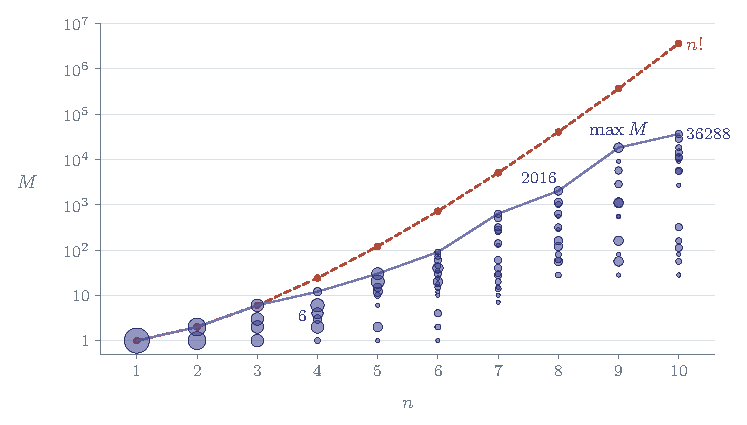
\includegraphics[width=0.85\textwidth]{fig_multiple}
\caption{\Cref{rem:themultiple}. The least multiple $M$ of
\Cref{thm:secantexists} for $1\le n\le10$, over the seventy-two cases
$d\in\{1,2,3,5,7,11\}$, $a\in\{1,2,3\}$, $b\in\{\pm1,\pm2\}$ for each
$n$, read off from the solution of the Vandermonde system, on a logarithmic
scale; the area of a disc counts the cases with that value. The solid line
joins the largest values and the dashed one is $n!$, which every $M$ divides
by the remark: the quotient of $\ZZ^{n+1}$ by the lattice of the
characters $(1,j,\dots,j^{n})$ of the powers of a line bundle is dual to the
integer-valued polynomials of degree at most $n$, spanned by the
$\binom{x}{k}$, whose coefficients have denominators dividing $n!$.}
\label{fig:multiple}
\end{figure}

\begin{figure}[htbp]
\centering
  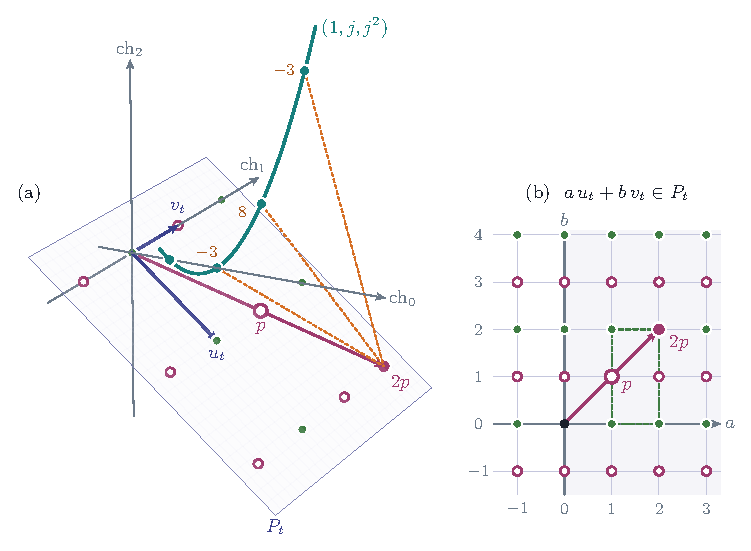
\includegraphics[width=0.86\textwidth]{fig_moment}
\caption{\Cref{thm:secantexists} at $n=2$ and $d=2$. (a) The coordinates
$(\ch_{0},\ch_{1},\ch_{2})$ in the basis $1$, $t$, $t^{2}/2$. The Chern
characters of the powers of one line bundle lie on the moment curve
$j\mapsto(1,j,j^{2})$, and the Vandermonde determinant says that any three of
its points are affinely independent. The integral points of
$P_{t}=\QQ u_{t}\oplus\QQ v_{t}$ split by the criterion
$\ch_{2}\equiv\ch_{1}\bmod2$ into those reached by integer combinations of
line bundles, drawn filled, and those missed, drawn open. The point
$p=u_{t}+v_{t}$ is missed and $2p$ is reached, by the witness
$-3[\cO_{X}]+8[\cO_{X}(t)]-3[\cO_{X}(2t)]$, whose three terms are joined to
$2p$ by dashed segments. (b) The same points in the coordinates $(a,b)$ of
$a\,u_{t}+b\,v_{t}$. Here $\ch_{1}=b$ and $\ch_{2}=-2a$, so the criterion reads
$b\equiv0\bmod2$; the shaded half-plane $a>0$ is the range of
\Cref{thm:secantexists}.}
\label{fig:moment}
\end{figure}

\subsection{The three ingredients}

\begin{theorem}[Three of the four ingredients]\label{thm:twoofthefour}
For every $n\ge2$, every squarefree $d>0$ and every polarised abelian $n$-fold
$X$ carrying a nondegenerate $\beta\in\NS(X)\otimes\QQ$, the first three of the
four ingredients required by \Cref{q:higher} exist and are explicit:
\begin{enumerate}[label=\textup{(\alph*)}]
\item the abelian $2n$-fold of Weil type is $A=X\times\widehat{X}$ with the
  $K$-action \eqref{eq:Mdef}, by \Cref{thm:explicitweil};
\item the plane is $P_{t}$ of \Cref{def:secantplane} with $t=\beta$, it is
  spanned by Hodge classes and it meets the spinor variety in exactly the two
  conjugate points $[e^{\pm st}]$, by \Cref{thm:plane};
\item a pair of coherent sheaves $\cF_{1},\cF_{2}$ on $X$ whose Chern
  characters are linearly independent rational points of $P_{t}$ exists, by
  \Cref{thm:secantexists}, and each may be taken to have the class of an
  explicit integer combination of powers of one line bundle.
\end{enumerate}
The invariants of any such sheaf are forced by the explicit system of
\Cref{thm:secantinvariants}, which imposes $n-1$ linear conditions on a Chern
character already constrained to $\QQ[t]$, and, when $\beta$ is ample, are
unobstructed numerically by \eqref{eq:discnorm}.
\end{theorem}

\begin{proof}
Items (a), (b) and (c) are the cited theorems. For (c), the proof of
\Cref{thm:secantexists} uses of $t$ only that $t^{n}\ne0$ and that a positive
multiple of $t$ is integral; both hold for $t=\beta$, the first because
$\beta$ is nondegenerate. For the count in the last sentence, a Chern
character in the subring $\QQ[t]\subset H^{\mathrm{ev}}(X,\QQ)$ is a
polynomial of degree at most $n$ in $t$, so lies in a space of dimension
$n+1$, while $P_{t}$ has dimension two, and $(n+1)-2=n-1$.
\end{proof}

\begin{remark}[The deformation step]\label{rem:deformation}
The fourth ingredient of \Cref{q:higher} is untouched by this section, and it
is the hardest. Given the pair of secant sheaves $\cF_{1},\cF_{2}$ on $X$
supplied by \Cref{thm:secantexists}, one must still show that the
characteristic class of $\Phi(\cF_{1}^{\vee}\boxtimes\cF_{2})$ remains of
Hodge type under every deformation of $X\times\widehat{X}$ as a polarised
abelian $2n$-fold of Weil type, and that the object deforms with the variety,
as a twisted sheaf to first order. Markman carries out this step at $n=3$
\cite{Mar25b}, through a semiregularity analysis. Our contribution to it is
negative: \Cref{thm:factor} identifies the Hochschild classes that the
weakened form of that analysis must kill for a secant object, and
\Cref{thm:candidatefails} shows that the candidate Markman proposes for $n=4$
does not kill them. Without the step one obtains algebraicity only on the
split locus $X\times\widehat{X}$, where the Weil classes are of much less
interest, since the general abelian $2n$-fold of Weil type is simple and is
not of that form.

Accordingly, nothing in this section proves the Hodge conjecture for abelian
$2n$-folds of Weil type at any $n\ge4$. What is established is that three of
the four ingredients are written down for every $n$, the third with an
explicit witness in line bundles, and that the fourth is isolated.
\end{remark}

\begin{figure}[htbp]
\centering
  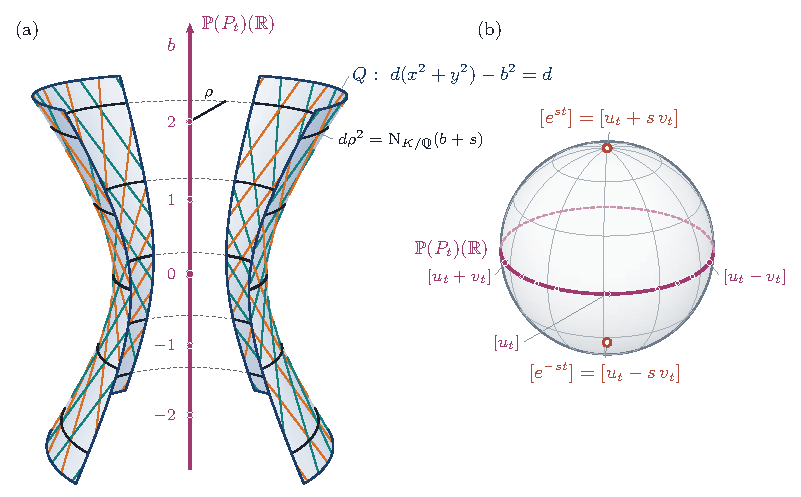
\includegraphics[width=0.88\textwidth]{fig_quadric}
\caption{The geometry of \Cref{thm:plane} in the first case, $n=2$. The even
spinor variety is then the smooth six-dimensional quadric of classes
isotropic for the Mukai pairing in $\PP(H^{\mathrm{ev}}(X,\CC))\cong\PP^{7}$,
and the figure shows a real two-dimensional section of it, a quadric surface
with its two rulings. The line $\PP(P_{t})$ of \Cref{def:secantplane} is
defined over $\QQ$ and meets the quadric only in the two points
$[e^{\pm st}]$, which are conjugate over $K$ and not individually rational;
they are drawn as real points. This is the configuration the Weil line
demands: a class defined over $\QQ$ cannot single out one of the two points,
so the construction must carry the pair, and the pair spans a plane rather
than a line. \Cref{prop:orbitplane} is the same statement on the
cohomological side, and \Cref{fig:escape} places it among the hypotheses a
construction can satisfy.}
\label{fig:spinor}
\end{figure}

\section{Base points in every Weil family}\label{sec:basepoints}

The secant construction of \Cref{sec:construction} lives on the split variety
$X\times\widehat{X}$ and stops short of the deformation step. In this section
we study the split member and the other special members of a Weil family
through the Weil classes themselves. On the split member the Weil classes are
polynomials in three divisor classes (\Cref{thm:splitclosed}); on products of
abelian surfaces of Weil type they are polynomials in divisor classes
(\Cref{thm:everyn}); and on abelian varieties with quaternionic
multiplication extending $K$, and on their products, they are polynomials in
two divisor classes, which yields an algebraic base point in every Weil
family, of every discriminant (\Cref{thm:everyfamily}). What remains is the
propagation of one flat class over one connected period domain, formulated
in \Cref{ssec:residual,ssec:exactform}.

\subsection{The split member in closed form}\label{ssec:split}

We begin with the split member, where a single formula, valid for every $n$
and every $d$, writes the Weil classes as polynomials in three divisor
classes. The split locus is thin. A general abelian $2n$-fold
of Weil type is simple, hence not isogenous to a product, and for $n\ge2$ the
members $X\times\widehat{X}$ form a subvariety of $\cD_{n,n}$ of positive
codimension (\Cref{prop:splitgeom}(iii)). \Cref{cor:splitalgebraic} is
therefore a base case, and \Cref{q:residual} is a question about propagation.

\begin{notation}\label{not:threeclasses}
On $A=X\times\widehat{X}$ write
\[
  \beta\in H^{2}(A,\QQ),
  \qquad
  \widehat{\beta}\in H^{2}(A,\QQ),
  \qquad
  \ell=c_{1}(\cP)\in H^{2}(A,\QQ)
\]
for the pullback of the polarisation of $X$, the pullback of the dual
polarisation of $\widehat{X}$, and the class of the Poincar\'e bundle. All
three are divisor classes, so every polynomial in them is algebraic. Put
\begin{equation}\label{eq:gammadef}
  \gamma=d\,\beta-\widehat{\beta}.
\end{equation}
\end{notation}

\begin{theorem}[The Weil line of the split member]\label{thm:splitclosed}
Let $A=X\times\widehat{X}$ carry the $K$-action \eqref{eq:Mdef} determined by a
principal $\beta$, and let $V_{\pm}\subset H^{1}(A,\CC)$ be the eigenspaces of
$\iota(\sqrt{-d})$. Then
\begin{enumerate}[label=\textup{(\roman*)},nosep]
\item $\gamma\mp\sqrt{-d}\,\ell$ lies in $\bigwedge^{2}V_{\pm}$, so it is an
  eigenclass for the character $\tau\mapsto\tau^{2}$ on $H^{2}(A,\CC)$
  respectively for its conjugate;
\item the generators of $\bigwedge^{2n}V_{\pm}$ are
  \begin{equation}\label{eq:splitclosed}
    \omega_{\pm}
    =\frac{(-1)^{n(n-1)/2}}{n!\,d^{\,n}}
      \bigl(\gamma\mp\sqrt{-d}\,\ell\bigr)^{n};
  \end{equation}
\item consequently the Weil line of $A$ is
  \[
    \HW(A)=\Bigl\langle\;
      \Re\bigl(\gamma-\sqrt{-d}\,\ell\bigr)^{n},\;\;
      \Im\bigl(\gamma-\sqrt{-d}\,\ell\bigr)^{n}
    \;\Bigr\rangle_{\QQ},
  \]
  and every Weil class on $A$ is a polynomial with rational coefficients in
  the three divisor classes $\beta,\widehat{\beta},\ell$, hence is algebraic.
\end{enumerate}
\end{theorem}

\begin{proof}
Write $U=H^{1}(X,\QQ)$ with basis $x_{1},\dots,x_{2n}$ chosen so that
$\beta=\sum_{j\le n}x_{j}\wedge x_{n+j}$, let $\xi_{1},\dots,\xi_{2n}$ be the
dual basis of $H^{1}(\widehat{X},\QQ)=U^{\vee}$, and let $B\colon U\to U^{\vee}$
be the isomorphism induced by $\beta$, so that $Bx_{j}=\xi_{n+j}$ and
$Bx_{n+j}=-\xi_{j}$. The endomorphism \eqref{eq:Mdef} acts on homology, and
its transpose $M^{*}$ acts on $H^{1}(A,\QQ)=U\oplus U^{\vee}$ by
$u\mapsto -Bu$ and $\phi\mapsto d\,B^{-1}\phi$. Indeed, in the basis
$u_{1},\dots,u_{2n}$ of $H_{1}(X,\QQ)$ dual to the $x_{i}$, the map
$\beta\colon H_{1}(X)\to H^{1}(X)$ sends $u_{j}\mapsto x_{n+j}$ and
$u_{n+j}\mapsto-x_{j}$, so \eqref{eq:Mdef} sends $u_{j}\mapsto dx_{n+j}$,
$u_{n+j}\mapsto-dx_{j}$, $x_{n+j}\mapsto-u_{j}$ and $x_{j}\mapsto u_{n+j}$,
where $x_{i}$ is regarded as an element of
$H_{1}(\widehat X,\QQ)=H^{1}(X,\QQ)$ and $\xi_{i}$ is its dual class; pairing
with the dual basis gives the stated action. The square of $M^{*}$ is $-d$;
so, writing $\delta=\sqrt{-d}$,
\begin{equation}\label{eq:splitVpm}
  V_{\pm}=\Bigl\{\,u\pm\tfrac{\delta}{d}\,Bu\;:\;u\in U_{\CC}\Bigr\},
\end{equation}
since $M^{*}\bigl(u\pm\tfrac{\delta}{d}Bu\bigr)
=-Bu\pm\delta u=\pm\delta\bigl(u\pm\tfrac{\delta}{d}Bu\bigr)$.

(i) Take the sum over $j\le n$ of the wedges of the two eigenvectors attached
to $x_{j}$ and to $x_{n+j}$:
\[
  \sum_{j=1}^{n}
  \Bigl(x_{j}\pm\tfrac{\delta}{d}Bx_{j}\Bigr)\wedge
  \Bigl(x_{n+j}\pm\tfrac{\delta}{d}Bx_{n+j}\Bigr)
  =\beta\pm\tfrac{\delta}{d}\Sigma-\tfrac{1}{d}\widehat{\beta},
\]
using $\delta^{2}=-d$, where
$\Sigma=\sum_{j}\bigl(x_{j}\wedge Bx_{n+j}+Bx_{j}\wedge x_{n+j}\bigr)$ and
$\sum_{j}Bx_{j}\wedge Bx_{n+j}=\sum_{j}\xi_{n+j}\wedge(-\xi_{j})
=\widehat{\beta}$. Now
\[
  \Sigma=\sum_{j=1}^{n}\bigl(x_{j}\wedge(-\xi_{j})
        +\xi_{n+j}\wedge x_{n+j}\bigr)
   =-\sum_{i=1}^{2n}x_{i}\wedge\xi_{i}=-\ell .
\]
So the displayed sum is $\tfrac1d\bigl(d\beta-\widehat{\beta}\mp\delta\ell\bigr)
=\tfrac1d(\gamma\mp\delta\ell)$. It is a sum of wedges of pairs of vectors of
$V_{\pm}$, hence lies in $\bigwedge^{2}V_{\pm}$, which proves (i); the
statement about characters is \Cref{prop:grading} at $(r,s)=(2,0)$ and
$(0,2)$.

(ii) By (i) the $n$-th power $(\gamma\mp\delta\ell)^{n}$ lies in
$\bigwedge^{2n}V_{\pm}$, which is a line by \Cref{prop:weilline}. It is
nonzero: expanding $\gamma\mp\delta\ell=d\beta-\widehat{\beta}\mp\delta\ell$,
the only term of the $n$-th power lying in $\bigwedge^{2n}U$ is
$d^{\,n}\beta^{n}$, and $\beta^{n}\ne0$ because $\beta$ is nondegenerate;
the remaining terms all involve at least one $\xi$, so no cancellation can
occur. Hence $(\gamma\mp\delta\ell)^{n}$ spans $\bigwedge^{2n}V_{\pm}$ and is a
scalar multiple of $\omega_{\pm}=\bigwedge_{i=1}^{2n}\bigl(x_{i}\pm\tfrac{\delta}{d}Bx_{i}\bigr)$.
To find the scalar, compare the components in $\bigwedge^{2n}U$: that of
$\omega_{\pm}$ is $x_{1}\wedge\cdots\wedge x_{2n}$, while
\[
  d^{\,n}\beta^{n}=d^{\,n}\,n!\bigwedge_{j=1}^{n}(x_{j}\wedge x_{n+j})
  =d^{\,n}\,n!\,(-1)^{n(n-1)/2}\,x_{1}\wedge\cdots\wedge x_{2n},
\]
the sign being that of the permutation carrying
$(1,n+1,2,n+2,\dots,n,2n)$ to $(1,2,\dots,2n)$. Inverting gives
\eqref{eq:splitclosed}.

(iii) The two displayed classes are the real and imaginary parts of
$(\gamma-\delta\ell)^{n}$, which up to the nonzero rational factor in
\eqref{eq:splitclosed} are $\omega_{-}+\omega_{+}$ and
$(\omega_{-}-\omega_{+})/\delta$; by \Cref{prop:weilline}(i) these span
$\HW(A)$ over $\QQ$. Expanding $(\gamma-\delta\ell)^{n}$ by the binomial
theorem and separating even from odd powers of $\delta$ writes each of them as
a rational polynomial in $\beta,\widehat{\beta},\ell$, because
$\delta^{2m}=(-d)^{m}$ and $\delta^{2m+1}=(-d)^{m}\delta$. Products of divisor
classes are algebraic, so both are algebraic.
\end{proof}

\begin{example}\label{ex:splitsmall}
The $2n$ classes $x_{1},\dots,x_{2n}$ form a $K$-basis of $H^{1}(A,\QQ)$, on
which $\sqrt{-d}$ acts by $x\mapsto-Bx$, so \eqref{eq:omegaprod} applies to
them; with \eqref{eq:splitclosed} it gives the integral generators of
\Cref{thm:explicitgens} for this basis in closed form,
\[
  \omega_{1}+\sqrt{-d}\,\omega_{2}
  =\frac{(-1)^{n(n-1)/2}}{n!}\,\bigl(\gamma+\sqrt{-d}\,\ell\bigr)^{n}.
\]
At $n=2$ this reads
\[
  \omega_{1}=\tfrac12\bigl(d\,\ell^{2}-\gamma^{2}\bigr),
  \qquad
  \omega_{2}=-\gamma\,\ell,
\]
and at $n=3$,
\[
  \omega_{1}=\tfrac12\,d\,\gamma\,\ell^{2}-\tfrac16\gamma^{3},
  \qquad
  \omega_{2}=\tfrac16\,d\,\ell^{3}-\tfrac12\gamma^{2}\ell,
\]
with $\gamma=d\beta-\widehat{\beta}$ throughout.
\end{example}

\begin{corollary}[Algebraicity on the split locus]\label{cor:splitalgebraic}
For every $n\ge1$, every squarefree $d>0$ and every principally polarised
abelian $n$-fold $X$, the Weil classes of $A=X\times\widehat{X}$ with the
$K$-action \eqref{eq:Mdef} are algebraic, and an algebraic representative is
given by \eqref{eq:splitclosed} as an explicit rational combination of
intersections of three divisors.
\end{corollary}

\begin{proof}
This is \Cref{thm:splitclosed}(iii), together with the Lefschetz theorem on
$(1,1)$ classes, which makes $\beta,\widehat{\beta},\ell$ algebraic, and the
fact that the algebraic classes form a subring of $H^{*}(A,\QQ)$.
\end{proof}

\begin{remark}[Consistency with the character obstruction]\label{rem:splitconsistent}
\Cref{cor:splitalgebraic} does not contradict \Cref{thm:character}. At the
split point $\NS(A)\otimes\QQ$ contains the three independent classes
$\beta,\widehat{\beta},\ell$, so the hypothesis
$\NS(A)\otimes\QQ=\QQ\eta$ of \Cref{prop:notpoly} fails, and this is the
situation of \Cref{rem:special}. What \Cref{thm:character} forbids is a
$\Kx$-eigenclass for the norm character meeting the Weil line, and
$\gamma\mp\sqrt{-d}\,\ell$ is an eigenclass for $\tau^{2}$ and for
$\bbar{\tau}^{2}$, not for the norm. The formula \eqref{eq:splitclosed} is
the first place in the paper where a class in the relevant eigenspace is
exhibited, and such a class exists because the split member has enough
divisors to build one.
\end{remark}

\subsection{Products of abelian surfaces}\label{ssec:products}

A second source of members with enough divisors is the product, an operation
that the Weil line respects. Throughout this subsection $K$ is fixed and all
Weil structures are taken with respect to it.

\begin{lemma}[Products of Weil type]\label{lem:prodweil}
Let $(A_{1},\iota_{1},\eta_{1})$ be of $(K,-1,n_{1})$-Weil type and
$(A_{2},\iota_{2},\eta_{2})$ of $(K,-1,n_{2})$-Weil type. Then
$A=A_{1}\times A_{2}$, with the diagonal action
$\iota=\iota_{1}\times\iota_{2}$ and the product polarisation
$\eta=p_{1}^{*}\eta_{1}+p_{2}^{*}\eta_{2}$, is of
$(K,-1,n_{1}+n_{2})$-Weil type.
\end{lemma}

\begin{proof}
Write $V_{i}=H^{1}(A_{i},\QQ)$, so $V=H^{1}(A,\QQ)=V_{1}\oplus V_{2}$ as
$K$-vector spaces and $\dim_{K}V=2n_{1}+2n_{2}$. The Rosati involution of the
product polarisation is the product of the two Rosati involutions, so it
restricts on $K$ to conjugation, which is the sign $-1$ of
\Cref{def:weiltype}. For the multiplicities, the Hodge decomposition of $V$ is
the direct sum of those of $V_{1}$ and $V_{2}$, and the eigenspace
decomposition is likewise $V_{\pm}=V_{1,\pm}\oplus V_{2,\pm}$. Hence
\[
  \dim_{\CC}V_{+}^{1,0}
  =\dim_{\CC}V_{1,+}^{1,0}+\dim_{\CC}V_{2,+}^{1,0}
  =n_{1}+n_{2},
\]
and the same for the other three, which is \Cref{lem:balanced} for
$n=n_{1}+n_{2}$.
\end{proof}

For an abelian variety $A$ of $(K,-1,n)$-Weil type and a $K$-basis of
$H^{1}(A,\QQ)$, let $\omega_{1}(A),\omega_{2}(A)$ be the generators of the
Weil line given by \eqref{eq:omegagens} in that basis, and write
\[
  \omega(A)=\omega_{1}(A)+\sqrt{-d}\,\omega_{2}(A)\;\in\;
  K\otimes_{\QQ}H^{2n}(A,\QQ)
\]
for the $K$-valued Weil class; by \eqref{eq:omegaprod} its image in
$H^{2n}(A,\CC)$ is $d^{-n}\prod_{j}(d\,x_{j}+\delta\,y_{j})$. On a product we
use the $K$-basis obtained by concatenating bases of the factors.

The Weil line is the top exterior power over $K$, and a top exterior power of
a direct sum is the tensor product of the top exterior powers. This is the
content of the next theorem; what has to be checked is its effect on the
rational generators, which are defined through the real structure rather
than over $K$.

\begin{theorem}[The Weil class is multiplicative]\label{thm:weilmult}
With the notation of \Cref{lem:prodweil}, and cup product on
$H^{*}(A,\QQ)$ taken after pullback along the two projections,
\begin{equation}\label{eq:weilmult}
\begin{aligned}
  \omega_{1}(A)&=\omega_{1}(A_{1})\,\omega_{1}(A_{2})
    -d\,\omega_{2}(A_{1})\,\omega_{2}(A_{2}),\\
  \omega_{2}(A)&=\omega_{1}(A_{1})\,\omega_{2}(A_{2})
    +\omega_{2}(A_{1})\,\omega_{1}(A_{2}),
\end{aligned}
\end{equation}
that is $\omega(A_{1})\,\omega(A_{2})=\omega(A_{1}\times A_{2})$ for the
$K$-valued Weil class. For $k$ factors,
$\prod_{j}\omega(A_{j})=\omega(A_{1}\times\cdots\times A_{k})$.
\end{theorem}

\begin{proof}
Let $u_{1},\dots,u_{2n_{1}}$ and $u_{2n_{1}+1},\dots,u_{2n}$ be the
$K$-bases of $H^{1}(A_{1},\QQ)$ and $H^{1}(A_{2},\QQ)$, so that together they
form the $K$-basis of $H^{1}(A,\QQ)$, and put $x_{j}=u_{j}$ and
$y_{j}=\sqrt{-d}\,u_{j}$ as in \eqref{eq:omegaprod}. By \eqref{eq:omegaprod},
\[
\begin{aligned}
  \omega(A)
  &=d^{-n}\prod_{j=1}^{2n}\bigl(d\,x_{j}+\delta\,y_{j}\bigr)\\
  &=\Bigl(d^{-n_{1}}\prod_{j\le2n_{1}}\bigl(d\,x_{j}+\delta\,y_{j}\bigr)\Bigr)
   \Bigl(d^{-n_{2}}\prod_{j>2n_{1}}\bigl(d\,x_{j}+\delta\,y_{j}\bigr)\Bigr)
  =\omega(A_{1})\,\omega(A_{2})
\end{aligned}
\]
in $H^{2n}(A,\CC)$, the products being taken in the order of the basis, so
that no sign arises. Expanding
$\bigl(\omega_{1}(A_{1})+\delta\omega_{2}(A_{1})\bigr)
\bigl(\omega_{1}(A_{2})+\delta\omega_{2}(A_{2})\bigr)$ with $\delta^{2}=-d$,
and comparing rational parts and $\delta$-parts, which is legitimate because
the classes $\omega_{j}(A_{i})$ are rational and $1,\delta$ are linearly
independent over $\QQ$, gives \eqref{eq:weilmult}. The statement for $k$
factors follows by induction.
\end{proof}

\Cref{fig:product} shows the multiplicativity and the loci it reaches.

\begin{corollary}[Algebraicity propagates along products]\label{cor:prodalg}
If the Weil classes of $A_{1}$ and of $A_{2}$ are algebraic, then so are those
of $A_{1}\times A_{2}$, and an algebraic representative is the rational
combination of external products given by \eqref{eq:weilmult}.
\end{corollary}

\begin{proof}
Algebraic classes are closed under pullback along the projections and under
cup product, and \eqref{eq:weilmult} expresses $\omega_{1}(A)$ and
$\omega_{2}(A)$ in those operations applied to the $\omega_{j}(A_{i})$.
\end{proof}

In dimension two there is nothing to prove.

\begin{lemma}[Dimension two]\label{lem:basecase}
Let $A_{0}$ be of $(K,-1,1)$-Weil type, so $\dim A_{0}=2$. Then
$\HW(A_{0})\subset H^{2}(A_{0},\QQ)$ and both generators are algebraic.
\end{lemma}

\begin{proof}
The Weil classes lie in $H^{2n}=H^{2}$ and are of type $(1,1)$ by
\Cref{prop:weilline}(ii), so they are algebraic by the Lefschetz theorem on
$(1,1)$ classes. No hypothesis on $A_{0}$ beyond the Weil structure is used.
\end{proof}

\begin{theorem}[An algebraic Weil class in every dimension]\label{thm:everyn}
Let $n\ge1$, let $d>0$ be squarefree, and let $A_{1},\dots,A_{n}$ be abelian
surfaces of $(K,-1,1)$-Weil type. Then $A=A_{1}\times\cdots\times A_{n}$ is of
$(K,-1,n)$-Weil type and its Weil classes are algebraic; explicitly, by
\Cref{thm:weilmult} and \Cref{lem:basecase} they are the rational part and
the coefficient of $\sqrt{-d}$ in
$\prod_{j=1}^{n}\bigl(\omega_{1}(A_{j})+\sqrt{-d}\,\omega_{2}(A_{j})\bigr)$,
a polynomial with integer coefficients in $2n$ divisor classes.
\end{theorem}

\begin{proof}
\Cref{lem:prodweil} gives the Weil structure, \Cref{lem:basecase} gives
algebraicity of each factor's classes, and \Cref{cor:prodalg} applied $n-1$
times gives the conclusion; the displayed form is \Cref{thm:weilmult} for $k=n$
factors. Each $\omega_{j}(A_{i})$ is a divisor class by
\Cref{lem:basecase}, so the product is a polynomial in $2n$ of them.
\end{proof}

\begin{remark}[The product locus]\label{rem:prodscope}
\Cref{thm:everyn} is unconditional and holds for every $n$; like
\Cref{cor:splitalgebraic} and \Cref{thm:everyfamily}, it produces an algebraic
Weil class in every dimension using nothing beyond the Lefschetz theorem on
$(1,1)$ classes. The product construction supplies a second family of base
points, defined for every $n$ and every $d$, at which the class is written
down explicitly. It also shows that the algebraicity locus is closed under
products, so that a settled case $n_{0}$ propagates to every multiple of
$n_{0}$, and settled cases propagate to their sums. Combined with Markman's
theorem at $n=2$ \cite{Mar25a,Mar25b}, this gives, for every $n$,
algebraicity on the locus of products of abelian fourfolds and surfaces of
Weil type, which has dimension $2n$ when $n$ is even.

The reach of these results is limited. The family of polarised abelian
$2n$-folds of $(K,-1,n)$-Weil type has dimension $n^{2}$, and the locus of
products of $n$ surfaces has dimension $n$, so for $n\ge2$ it is a proper
closed subvariety, smaller than the quaternionic locus of \Cref{thm:quatweil},
whose dimension is $n(n+1)/2$. A general member of the family is simple,
hence not isogenous to a product, and neither \Cref{thm:everyn} nor
\Cref{cor:splitalgebraic} applies to it. The general member lies outside all
of these loci, and by \Cref{thm:residual} what joins them to it is the
propagation statement.
\end{remark}

\begin{figure}[htbp]
\centering
  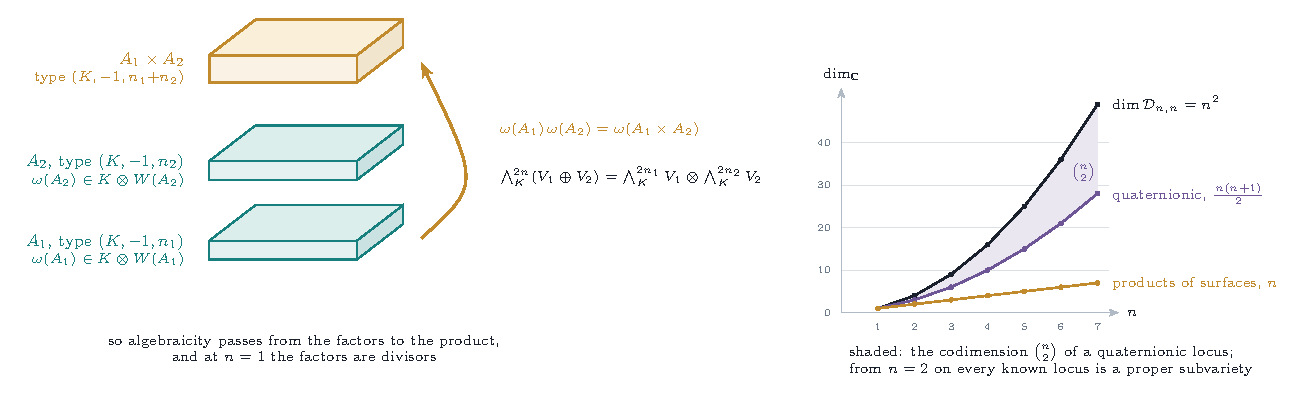
\includegraphics[width=0.96\textwidth]{fig_product}
\caption{\Cref{thm:weilmult} and its reach. Left: the Weil line of each factor
is a $K$-line, the Weil line of the product is the tensor product of the two
over $K$, and the $K$-valued Weil class is multiplicative. Algebraicity therefore passes from the factors to the product, and
at $n=1$ the factors are divisor classes, so a product of $n$ abelian surfaces
of Weil type carries an explicit algebraic Weil class in every dimension.
Right: the dimensions of the loci on which the class is known to be algebraic,
against the dimension $n^{2}$ of the family. Both the quaternionic locus and
the product locus are proper subvarieties once $n\ge2$, and a general member
lies on neither.}
\label{fig:product}
\end{figure}

\subsection{The residual statement}\label{ssec:residual}

The results above allow the remaining question to be stated in one sentence,
without auxiliary hypotheses.

\begin{setupenv}[The family]\label{setup:family}
Fix $n\ge2$ and a squarefree $d>0$. Let $\cD_{n,n}$ be the period domain of
\Cref{prop:weildomain} and let
\[
  \pi\colon\cA\longrightarrow\cD_{n,n}
\]
be the family of polarised abelian $2n$-folds of $(K,-1,n)$-Weil type it
parametrises, with $\omega$ the flat section of $R^{2n}\pi_{*}\QQ$ given
fibrewise by the class $\omega_{1}$ of \eqref{eq:omegagens}. Let
$\cD^{\mathrm{spl}}\subset\cD_{n,n}$ be the locus of split members
$X\times\widehat{X}$ carrying the action \eqref{eq:Mdef}.
\end{setupenv}

\begin{question}[The residual statement]\label{q:residual}
Is $\omega_{s}$ algebraic for every $s\in\cD_{n,n}$?
\end{question}

\begin{theorem}[The reduction]\label{thm:residual}
Fix $n\ge2$ and a squarefree $d>0$, and keep the notation of
\Cref{setup:family}.
\begin{enumerate}[label=\textup{(\alph*)},nosep]
\item If \Cref{q:residual} has a positive answer, then the Hodge conjecture
  holds, in every degree, for every abelian $2n$-fold of $(K,-1,n)$-Weil type
  with $\Hg(A)=\SU(V,H)$.
\item Conversely, if the Hodge conjecture holds for every abelian $2n$-fold of
  $(K,-1,n)$-Weil type, then \Cref{q:residual} has a positive answer.
\item $\cD^{\mathrm{spl}}$ is nonempty, $\omega_{s}$ is algebraic at every
  $s\in\cD^{\mathrm{spl}}$ with the explicit representative
  \eqref{eq:splitclosed}, and $\cD_{n,n}$ is connected.
\end{enumerate}
Thus \Cref{q:residual} is the variational Hodge conjecture for one flat class
on one connected family; it is necessary as well as sufficient, and its base
case is supplied. \Cref{thm:everyfamily} supplies a base case in every family,
for every discriminant, so nonemptiness of the base locus is never the
obstacle.
\end{theorem}

\begin{proof}
(a) Let $A$ be of $(K,-1,n)$-Weil type with $\Hg(A)=\SU(V,H)$. By
\Cref{prop:weildomain} its Hodge structure is a point $s$ of $\cD_{n,n}$, so
$A$ is a fibre of $\pi$, and the Weil line of $A$ is generated over $K$ by
$\omega_{s}$. A positive answer makes $\omega_{s}$ algebraic, hence makes the
whole Weil line algebraic by the argument of \Cref{cor:whatisleft}. By
\Cref{thm:hdgcount} the Weil line together with the powers of $\eta$ exhausts
$\Hdg^{*}(A)$, and the powers of $\eta$ are algebraic, so every Hodge class on
$A$ is algebraic.

(b) For every $s$ the class $\omega_{s}$ is a Hodge class on the fibre $A_{s}$,
by \Cref{prop:weilline}(ii), and $A_{s}$ is of $(K,-1,n)$-Weil type by
construction. So the Hodge conjecture for $A_{s}$ gives its algebraicity.

(c) $\cD^{\mathrm{spl}}$ is nonempty because the construction \eqref{eq:Mdef}
applies to any principally polarised abelian $n$-fold and produces a point of
$\cD_{n,n}$ by \Cref{thm:explicitweil}; algebraicity there is
\Cref{cor:splitalgebraic}; and $\cD_{n,n}$ is connected because it is a
bounded symmetric domain, by \Cref{prop:weildomain}.
\end{proof}

\begin{remark}[The target]\label{rem:target}
The preceding sections remove three parts of the problem.
\Cref{thm:hdgcount} settles how many classes are at issue: one, in one
degree, on each fibre. \Cref{thm:divisor} and \Cref{thm:character} exclude
two families of candidate constructions. \Cref{thm:splitclosed} supplies the
base case: the class is algebraic somewhere in the family, with a
representative that can be written on a single line.

The next step is propagation, which is Grothendieck's variational Hodge
conjecture for the pair $(\pi,\omega)$ of \Cref{setup:family}.
\Cref{thm:residual} shows that for the Hodge conjecture on
abelian varieties of Weil type it is necessary as well as sufficient, so every
route to the conjecture meets an equivalent difficulty.
\Cref{ssec:properness} analyses the propagation; there the passage from a
formal deformation to an algebraic one, usually the harder half, is supplied
by properness of the Hilbert scheme. What survives is either an infinitesimal
statement at a single point or a bound on the complexity of representing
cycles along one orbit, and the second is equivalent to its conclusion
(\Cref{thm:p1equivalent}).
\end{remark}

\subsection{The divisorial criterion}
\label{ssec:divcrit}

\Cref{thm:splitclosed} is a computation on one member of the family, but the
mechanism behind it is not special to that member. Isolating it gives a
criterion that can be tested at any point; we then determine where it holds.

\begin{theorem}[The divisorial criterion]\label{thm:divcriterion}
Let $(A,\iota,\eta)$ be of $(K,-1,n)$-Weil type and suppose there exists
$\Theta\in\bigwedge^{2}V_{-}$ with
\begin{enumerate}[label=\textup{(\roman*)},nosep]
\item $\Theta$ nondegenerate as an alternating form on $V_{-}^{\vee}$,
  equivalently $\Theta^{n}\ne0$;
\item $\Theta$ of Hodge type $(1,1)$;
\item $\Theta+\bbar{\Theta}$ rational, that is in $H^{2}(A,\QQ)$.
\end{enumerate}
Then the Weil classes of $A$ are algebraic. Explicitly, writing
$g=\Theta+\bbar{\Theta}$ and $\lambda=(\Theta-\bbar{\Theta})/\sqrt{-d}$, both
$g$ and $\lambda$ are divisor classes and
\begin{equation}\label{eq:divrep}
  \HW(A)=\Bigl\langle\;
    \Re\bigl(g+\sqrt{-d}\,\lambda\bigr)^{n},\;\;
    \Im\bigl(g+\sqrt{-d}\,\lambda\bigr)^{n}\;\Bigr\rangle_{\QQ},
\end{equation}
so every Weil class is a rational polynomial in two divisor classes.
\end{theorem}

\begin{proof}
Conjugation interchanges $\bigwedge^{2}V_{-}$ and $\bigwedge^{2}V_{+}$, so
$\bbar{\Theta}\in\bigwedge^{2}V_{+}$, and both $g$ and $\lambda$ are fixed by
conjugation, hence real. Rationality of $g$ is (iii); that of $\lambda$
comes from the action of $\Kx$. Fix
$\tau=a+b\sqrt{-d}\in\Kx$ with $ab\ne0$. By \Cref{prop:grading} the operator
$\iota(\tau)^{*}$ acts on $\bigwedge^{2}V_{+}$ by $\tau^{2}=a^{2}-db^{2}+2ab\sqrt{-d}$
and on $\bigwedge^{2}V_{-}$ by $\bbar{\tau}^{\,2}$, so
\[
  J:=\frac{\iota(\tau)^{*}-(a^{2}-db^{2})}{2ab}
\]
is a $\QQ$-rational endomorphism of $H^{2}(A,\QQ)$ preserving the space $R$
of \Cref{prop:normpart} and acting
on $\bigwedge^{2}V_{\pm}$ by $\pm\sqrt{-d}$. Applying it to
$g=\Theta+\bbar{\Theta}$ gives $J(g)=-\sqrt{-d}\,\Theta+\sqrt{-d}\,\bbar{\Theta}
=-\sqrt{-d}\cdot\sqrt{-d}\,\lambda=d\,\lambda$, so $\lambda=J(g)/d$ is
rational. Both $g$ and $\lambda$ are of type $(1,1)$ by (ii) and conjugation
symmetry, so both lie in $\NS(A)\otimes\QQ$ by the Lefschetz theorem on
$(1,1)$ classes, and both are algebraic.

By (i) the form $\Theta$ on the $2n$-dimensional space $V_{-}$ has nonzero
Pfaffian, so $\Theta^{n}$ is a nonzero element of the line
$\bigwedge^{2n}V_{-}$, and it therefore spans it; conjugating,
$\bbar{\Theta}^{\,n}$ spans $\bigwedge^{2n}V_{+}$. Hence
$\Theta^{n}+\bbar{\Theta}^{\,n}$ and
$(\Theta^{n}-\bbar{\Theta}^{\,n})/\sqrt{-d}$ span $\HW(A)$ over $\QQ$, by
\Cref{prop:weilline}(i). Finally
$2^{n}\Theta^{n}=(g+\sqrt{-d}\lambda)^{n}$, and expanding by the binomial
theorem with $(\sqrt{-d})^{2m}=(-d)^{m}$ writes the real and imaginary parts
as rational polynomials in $g$ and $\lambda$. Products of divisor classes are
algebraic.
\end{proof}

\begin{corollary}\label{cor:splitsatisfies}
The split member of \Cref{thm:splitclosed} satisfies the criterion, with
$\Theta=\gamma-\sqrt{-d}\,\ell$ and $\gamma=d\beta-\widehat{\beta}$; the two
divisor classes of \eqref{eq:divrep} are $2\gamma$ and $-2\ell$.
\end{corollary}

\begin{proof}
\Cref{thm:splitclosed}(i) places $\Theta=\gamma-\sqrt{-d}\,\ell$ in
$\bigwedge^{2}V_{+}$ and its conjugate in $\bigwedge^{2}V_{-}$. The hypotheses
and the conclusion of \Cref{thm:divcriterion} are symmetric under replacing
$\Theta$ by $\bbar{\Theta}$, which interchanges $V_{+}$ and $V_{-}$, fixes $g$
and changes the sign of $\lambda$, so the criterion may be applied to
$\Theta$. The classes $\gamma$ and $\ell$ are divisor classes, hence of type
$(1,1)$, so $\Theta$ is of type $(1,1)$ and $\Theta+\bbar{\Theta}=2\gamma$ is
rational. Nondegeneracy is the nonvanishing of $\Theta^{n}$, proved in
\Cref{thm:splitclosed}(ii).
\end{proof}

The base case is therefore one instance of a general criterion. The next two
results determine how far the criterion reaches, and both limit it.

\begin{proposition}[The criterion fails at a general point]\label{prop:divfails}
Let $(A,\iota,\eta)$ be of $(K,-1,n)$-Weil type with $n\ge2$ and
$\Hg(A)=\SU(V,H)$. Put
\[
  R=\Bigl(\textstyle\bigwedge^{2}V_{+}\oplus\bigwedge^{2}V_{-}\Bigr)
      \cap H^{2}(A,\QQ).
\]
Then $R\cap\NS(A)_{\QQ}=0$, and no $\Theta$ as in \Cref{thm:divcriterion}
exists.
\end{proposition}

\begin{proof}
By \Cref{prop:normpart} the space $R$ is a rational sub-Hodge structure of
$H^{2}(A,\QQ)$, and the intersection $R\cap\NS(A)_{\QQ}$ is a rational
sub-Hodge structure of $R$ of pure type $(1,1)$. The complexification of a
nonzero rational sub-Hodge structure of $R$ is a nonzero
$\Hg(A)_{\CC}$-subrepresentation of $\bigwedge^{2}V_{+}\oplus\bigwedge^{2}V_{-}$,
so it contains a constituent isomorphic to $\bigwedge^{2}V_{+}$ or to
$\bigwedge^{2}V_{-}$; by the proof of \Cref{prop:normpart}, Hodge numbers
depend only on the representation, and by \Cref{prop:h2pieces} each of
$\bigwedge^{2}V_{\pm}$ has $h^{2,0}+h^{0,2}=2\binom{n}{2}=n(n-1)$, which is
positive for $n\ge2$. So no nonzero rational sub-Hodge structure of $R$ is of
pure type $(1,1)$, and $R\cap\NS(A)_{\QQ}=0$. The argument covers the case
$n=2$ with trivial discriminant, where $R$ is reducible. A $\Theta$ as in
\Cref{thm:divcriterion} would give the nonzero element $\Theta+\bbar{\Theta}$
of $R\cap\NS(A)_{\QQ}$.
\end{proof}

\begin{proposition}[The split locus]\label{prop:splitgeom}
Fix $n\ge1$ and a squarefree $d>0$, and let $A=X\times\widehat{X}$ carry the
$K$-action \eqref{eq:Mdef} determined by a nondegenerate
$\beta\in\NS(X)\otimes\QQ$ of elementary divisors $(d_{1},\dots,d_{n})$.
\begin{enumerate}[label=\textup{(\roman*)},nosep]
\item Let $B$ be the Gram matrix of $\beta$ in a basis of $U$, and let
  $\widehat\beta$ be the form on $U^{\vee}$ with Gram matrix $-B^{-1}$ in the
  dual basis, which for principal $\beta$ is the class of
  \Cref{not:threeclasses}. The polarisation of $A$ is
  $\eta=\beta+\widehat{\beta}/d$, a positive rational multiple of
  $d\beta+\widehat\beta$; its Gram matrix on $H_{1}(A,\QQ)=U\oplus U^{\vee}$
  is the block form $Q=B\oplus(-B^{-1}/d)$, and $M$ is anti-self-adjoint for
  it.
\item In the $K$-basis $u_{1},\dots,u_{2n}$ of $H_{1}(A,\QQ)$ the hermitian
  form of \Cref{lem:hermform} has Gram matrix $\sqrt{-d}\,B$, so
  \[
    \det H=(-d)^{n}\det B=(-d)^{n}(d_{1}\cdots d_{n})^{2},
  \]
  and $(-1)^{n}\det H=d^{\,n}(d_{1}\cdots d_{n})^{2}$ is a norm from $K$.
  Every split member therefore lies in the Weil family of trivial
  discriminant, whatever $\beta$ is chosen.
\item The split members form a locus of dimension $n(n+1)/2$ inside
  $\cD_{n,n}$, of codimension $n(n-1)/2$, which is zero only for $n=1$ and is
  a divisor for $n=2$.
\item For $X$ with $\Hg(X)=\mathrm{Sp}(H^{1}(X,\QQ))$ one has
  $\NS(A)_{\QQ}=\langle\beta,\widehat{\beta},\ell\rangle$, of rank three, and
  in degree $2n$ the monomials in those three classes span the whole space of
  Hodge classes of $A$.
\end{enumerate}
\end{proposition}

\begin{proof}
(i) In the chosen basis of $U$ and the dual basis of $U^{\vee}$ the map
$\beta\colon U\to U^{\vee}$ has matrix $B^{\top}=-B$ and its inverse has
matrix $-B^{-1}$, so \eqref{eq:Mdef} becomes
$M=\begin{psmallmatrix}0&B^{-1}\\-dB&0\end{psmallmatrix}$, with
$M^{2}=-d$ and
$M^{\top}=\begin{psmallmatrix}0&dB\\-B^{-1}&0\end{psmallmatrix}$, using
$B^{\top}=-B$ and $(B^{-1})^{\top}=-B^{-1}$. For a block form
$Q=\begin{psmallmatrix}P&\Lambda\\-\Lambda^{\top}&S\end{psmallmatrix}$ the
Rosati relation $M^{\top}Q+QM=0$ reads
$B\Lambda^{\top}+\Lambda B=0$, $dBS+PB^{-1}=0$, $B^{-1}P+dSB=0$ and
$B^{-1}\Lambda+\Lambda^{\top}B^{-1}=0$. Taking $\Lambda=0$ and $P=B$ forces
$S=-B^{-1}/d$ from the second relation, and the third then reads $-I+I=0$.
So $Q=B\oplus(-B^{-1}/d)$, which is the Gram matrix of
$\beta+\widehat\beta/d$. For principal $\beta$ one may take
$B=\begin{psmallmatrix}0&I\\-I&0\end{psmallmatrix}$, so that $-B^{-1}=B$
and $\widehat\beta=\sum_{j}\xi_{j}\wedge\xi_{n+j}$ as in
\Cref{not:threeclasses}.

(ii) The set $u_{1},\dots,u_{2n}$ is a $K$-basis because
$MU=d\beta(U)=U^{\vee}$, and $H(u_{i},u_{j})=Q(Mu_{i},u_{j})+\sqrt{-d}\,Q(u_{i},u_{j})$
by \eqref{eq:QfromH}; the first term vanishes since $Mu_{i}\in U^{\vee}$,
$u_{j}\in U$ and $Q$ has no cross block by (i), and the second is
$\sqrt{-d}\,\beta_{ij}$. Hence the Gram matrix is $\sqrt{-d}\,B$ and
$\det H=(\sqrt{-d})^{2n}\det B=(-d)^{n}\det B$. The determinant of an
alternating matrix is the square of its Pfaffian, here $(d_{1}\cdots
d_{n})^{2}$. Now $d=\Nm_{K/\QQ}(\sqrt{-d})$ is a norm and every square is a
norm, and the norms form a subgroup of $\QQ^{\times}$, so
$d^{\,n}(d_{1}\cdots d_{n})^{2}$ is a norm.

(iii) A split member is determined by $X$ together with $\beta$; the moduli
space of polarised abelian $n$-folds has dimension $\dim\cA_{n}=n(n+1)/2$,
and the type of $\beta$ is discrete. By \Cref{prop:weildomain} the ambient domain has
dimension $n^{2}$, and $n^{2}-n(n+1)/2=n(n-1)/2$.

(iv) The Hodge classes of $A=X\times\widehat{X}$ are the invariants of
$\Hg(A)=\Hg(X)=\mathrm{Sp}(U)$ acting on
$\bigwedge^{*}(U\oplus U^{\vee})$. In degree two the invariants are the three
lines spanned by $\beta$, $\widehat{\beta}$ and $\ell$, one from each
K\"unneth summand $\bigwedge^{2}U$, $U\otimes U^{\vee}$ and
$\bigwedge^{2}U^{\vee}$. In higher degree, identify $U^{\vee}$ with $U$
through $\beta$, so that $\bigwedge^{*}(U\oplus U^{\vee})\cong
\bigwedge^{*}(U\otimes\QQ^{2})$ as representations of $\mathrm{Sp}(U)$. By the
first fundamental theorem of invariant theory for the symplectic group, the
invariants of $\mathrm{Sp}(U)$ in $U^{\otimes2m}$ are spanned by the tensors
attached to the pairings of the $2m$ factors, each a product of copies of the
invariant element of $U\otimes U$ dual to $\beta$. The projection of
$(U\otimes\QQ^{2})^{\otimes2m}$ onto $\bigwedge^{2m}(U\otimes\QQ^{2})$ is
equivariant and surjective, hence surjective on invariants since
$\mathrm{Sp}(U)$ is reductive, and it carries such a tensor, tensored with
vectors of $\QQ^{2}$, to a product of invariants of degree two. So the
invariants are generated by $\beta$, $\widehat{\beta}$ and $\ell$, and in
degree $2n$ the monomials $\beta^{i}\widehat{\beta}^{j}\ell^{k}$ with
$i+j+k=n$ span the Hodge classes.
\end{proof}

\begin{remark}[Two residual questions]\label{rem:residualmap}
The Weil families for a fixed $K$ and a fixed $n$ are classified by the
discriminant of the hermitian form, an element of the infinite group
$\QQ^{\times}_{>0}/\Nm_{K/\QQ}(K^{\times})$. By \Cref{prop:splitgeom}(ii) the
split construction of \Cref{ssec:split} produces a base point in only one of
them, the family of trivial discriminant; products of abelian surfaces of
Weil type (\Cref{thm:everyn}, \Cref{lem:products}) reach every discriminant,
but only on a locus of dimension $n$. Read together with
\Cref{thm:residual}, this divides \Cref{q:residual} into two questions of
different kinds.
\begin{enumerate}[label=\textup{(R\arabic*)},leftmargin=2.8em,itemsep=2pt]
\item \emph{Trivial discriminant.} A base point exists, with the explicit
  cycle \eqref{eq:splitclosed}, and what is missing is propagation off a locus
  of codimension $n(n-1)/2$. At $n=2$ that locus is a divisor and the
  propagation is known, by Markman \cite{Mar25a,Mar25b} and by Floccari and Fu
  \cite{FF26}; combined with \Cref{thm:residual}(a) this recovers the Hodge
  conjecture for abelian fourfolds of Weil type of trivial discriminant with
  full Hodge group. At $n=3$ it is settled as well, by Markman's theorem on
  the sixfolds of trivial discriminant \cite{Mar25a,Mar25b}, for every $K$.
  For $n\ge4$ it is the propagation statement, and by \Cref{prop:descent}
  it is then the only question in the imaginary quadratic case.
\item \emph{Nontrivial discriminant.} The split construction never lands
  there, by \Cref{prop:splitgeom}(ii), so it supplies no base
  point; and by \Cref{prop:divfails} no divisorial argument can supply one at
  a general member. A base point must come from a special member at which $R$
  acquires Hodge classes.
\end{enumerate}
Question (R2) is settled in \Cref{ssec:everyfamily}: the special members
required are built from abelian varieties with quaternionic multiplication
extending $K$ and their products, they exist in every family, and on them
\Cref{thm:divcriterion} applies. What then remains is the propagation
question of (R1), posed in every family, each of which has a base point.
\end{remark}

\begin{remark}[Codimension of the split locus]
\label{rem:nlcodim}
A component of the Noether--Lefschetz locus of a weight two variation has
codimension at most $h^{2,0}$, here $n(n-1)$. The split locus has codimension
$n(n-1)/2$ by \Cref{prop:splitgeom}(iii), half of that, so it is a
component of half the expected codimension. This reflects
\Cref{prop:splitgeom}(iv): at a split point $R$ acquires two independent Hodge
classes at once, namely $\gamma$ and $\ell$, and each of them costs
$h^{2,0}/2$ conditions rather than $h^{2,0}$. Whether there are components
of the expected codimension carrying only one class, and whether the
criterion of \Cref{thm:divcriterion} can be met on them, is not needed
below: question (R2) is answered in \Cref{ssec:everyfamily}
through quaternionic multiplication.
\end{remark}

\subsection{A base point in every family}\label{ssec:everyfamily}

By \Cref{prop:splitgeom}(ii) the split construction reaches a single
discriminant class. \Cref{thm:divcriterion} does not depend on the origin of
$\Theta$, and in this subsection $\Theta$ comes from an endomorphism rather
than from a pair of divisors chosen by hand. This source reaches every class,
and it settles question (R2) of \Cref{rem:residualmap}.

\begin{definition}[Discriminant]\label{def:disc}
For $(A,\iota,\eta)$ of $(K,-1,n)$-Weil type with hermitian form $H$ as in
\Cref{lem:hermform}, the \emph{discriminant} is the class of
$(-1)^{n}\det H$ in $\QQ^{\times}_{>0}/\Nm_{K/\QQ}(K^{\times})$. The sign
makes the representative positive, because $H$ has signature $(n,n)$; and the
class is well defined because changing the $K$-basis multiplies $\det H$ by a
norm. Hermitian forms of rank $2n$ over $K$ with signature $(n,n)$ are
classified by this class, so it labels the Weil families.
\end{definition}

The classes that enter \Cref{thm:divcriterion} have a description by
endomorphisms: a class in $R\cap\NS(A)_{\QQ}$ is the same thing as a
symmetric endomorphism that conjugates $K$.

\begin{lemma}[Classes in $R$ and endomorphisms]\label{lem:Rendomorphism}
Let $(A,\iota,\eta)$ be of $(K,-1,n)$-Weil type. The map $\mu\mapsto
g_{\mu}$, $g_{\mu}(x,y)=\eta(\mu x,y)$, is a bijection between
\begin{enumerate}[label=\textup{(\alph*)},nosep]
\item the elements $\mu\in\End^{0}(A)$ with $\mu^{\dagger}=\mu$ and
  $\mu\,\iota(\tau)=\iota(\bbar{\tau})\,\mu$ for all $\tau\in K$, and
\item the elements of $R\cap\NS(A)_{\QQ}$.
\end{enumerate}
Under it, $\mu$ invertible corresponds to $g_{\mu}$ nondegenerate, hence to a
nondegenerate $\Theta$. If such a $\mu\ne0$ exists and the centraliser of
$\iota(K)$ in $\End^{0}(A)$ is $\iota(K)$, then $\mu^{2}\in\QQ^{\times}$ and
$\iota(K)+\iota(K)\mu$ is a quaternion algebra $(-d,\mu^{2})_{\QQ}$ inside
$\End^{0}(A)$.
\end{lemma}

\begin{proof}
A class in $\NS(A)_{\QQ}$ is a symmetric homomorphism $A\to\Av$ up to isogeny,
that is $\eta\mu$ with $\mu^{\dagger}=\mu$. The condition
$g_{\mu}(\iota(\tau)x,y)=g_{\mu}(x,\iota(\tau)y)$, which says that $g_{\mu}$ is
$K$-bilinear and hence lies in $R=\bigwedge^{2}_{K}V$, reads
$\eta(\mu\iota(\tau)x,y)=\eta(\mu x,\iota(\tau)y)=\eta(\iota(\tau)^{\dagger}\mu
x,y)=\eta(\iota(\bbar{\tau})\mu x,y)$, using \Cref{def:weiltype}(iii), so it
is the condition $\mu\iota(\tau)=\iota(\bbar{\tau})\mu$. For the last sentence,
$\mu^{2}$ commutes with $\iota(K)$, hence lies in $\iota(K)$ by hypothesis, and
$\mu\mu^{2}\mu^{-1}=\mu^{2}$ forces it to be fixed by conjugation, so
$\mu^{2}\in\QQ^{\times}$. Then $\iota(\sqrt{-d})$ and $\mu$ generate the
quaternion algebra with the stated invariants.
\end{proof}

The criterion therefore asks for quaternionic multiplication extending $K$.
Abelian varieties with this structure are easy to construct, and their
invariants can be computed.

\begin{setupenv}[The quaternionic model]\label{setup:quat}
Let $b\in\QQ_{>0}$ and let $B=(-d,b)_{\QQ}$ be the quaternion algebra with
basis $1,i,j,ij$ and $i^{2}=-d$, $j^{2}=b$, $ij=-ji$. Let
$V=B^{n}$ as a left $B$-module, of dimension $4n$ over $\QQ$, let
$K=\QQ(i)\subset B$ act through $i$, and fix $a_{1},\dots,a_{n}\in\QQ^{\times}$
and
\begin{equation}\label{eq:quatE}
  E(x,y)=\sum_{k=1}^{n}a_{k}\,\mathrm{trd}\bigl(\bbar{x_{k}}\,i\,y_{k}\bigr),
\end{equation}
where $\mathrm{trd}$ is the reduced trace and $\bbar{\phantom{x}}$ the
canonical involution of $B$.
\end{setupenv}

\begin{theorem}[Weil type from quaternionic multiplication]\label{thm:quatweil}
With the data of \Cref{setup:quat}:
\begin{enumerate}[label=\textup{(\roman*)},nosep]
\item $E$ is alternating and nondegenerate, and its Rosati involution is
  $\beta\mapsto i^{-1}\bbar{\beta}i$, which restricts to complex conjugation on
  $K$ and fixes $j$; it is positive, the form $\mathrm{trd}(\beta\beta^{\dagger})$
  being diagonal with entries $2,2d,2b,2db$ on the basis;
\item in the $K$-basis $e_{1},e_{1}j,\dots,e_{n},e_{n}j$ of $V$ the hermitian
  form of \Cref{lem:hermform} is
  \[
    H=\mathrm{diag}\bigl(2a_{1}d,\,-2a_{1}bd,\;\dots,\;2a_{n}d,\,-2a_{n}bd\bigr),
  \]
  of signature $(n,n)$;
\item there is a complex structure on $V_{\RR}$ commuting with $B$ and
  polarised by $E$, and for every such the resulting abelian variety $A$ is of
  $(K,-1,n)$-Weil type, the balanced signature being forced rather than
  imposed;
\item the discriminant of $A$ is the class of $b^{n}$;
\item $\mu=$ left multiplication by $j$ satisfies \Cref{lem:Rendomorphism}(a),
  so $g=g_{\mu}$ lies in $R\cap\NS(A)_{\QQ}$ and is nondegenerate, the
  divisorial criterion \Cref{thm:divcriterion} applies, and the Weil classes
  of $A$ are algebraic.
\end{enumerate}
\end{theorem}

\begin{proof}
(i) $\mathrm{trd}(z)=\mathrm{trd}(\bbar{z})$ and
$\overline{\bbar{x}iy}=\bbar{y}\,\bbar{i}\,x=-\bbar{y}ix$ give
$E(y,x)=-E(x,y)$. Nondegeneracy is the nondegeneracy of the reduced trace
pairing. For the Rosati, $E(\beta x,y)=E(x,\beta^{\dagger}y)$ for all $x,y$
reads $\bbar{\beta}i=i\beta^{\dagger}$, that is
$\beta^{\dagger}=i^{-1}\bbar{\beta}i$. Then $i^{\dagger}=-i$ and, since
$(-j)i=ij$, also $j^{\dagger}=i^{-1}(ij)=j$. Positivity is the displayed
diagonal, which is positive because $d>0$ and $b>0$.

(ii) $V=Ke_{k}\oplus Ke_{k}j$ over all $k$, since $B=K\oplus Kj$. By
\eqref{eq:QfromH}, $H(x,y)=E(ix,y)+\sqrt{-d}\,E(x,y)$. On one factor,
$E(ix,y)=a\,\mathrm{trd}(\overline{ix}\,i\,y)=-a\,\mathrm{trd}(\bbar{x}i^{2}y)
=ad\,\mathrm{trd}(\bbar{x}y)$, so
\[
  H(x,y)=a\bigl[d\,\mathrm{trd}(\bbar{x}y)+\sqrt{-d}\,\mathrm{trd}(\bbar{x}iy)\bigr].
\]
Now $\mathrm{trd}(1)=2$, $\mathrm{trd}(i)=\mathrm{trd}(j)=\mathrm{trd}(ij)=0$,
$\bbar{j}j=-b$ and $\bbar{j}ij=ib$, which give $H(1,1)=2ad$,
$H(j,j)=-2abd$ and $H(1,j)=0$. Since $b>0$ the two entries of each block have
opposite signs, so the signature is $(n,n)$.

(iii) A complex structure commuting with $B$ and compatible with $E$ is the
same as a subspace $V^{1,0}\subset V_{\CC}$, stable under $B$, with
$V_{\CC}=V^{1,0}\oplus\overline{V^{1,0}}$ and the two Riemann relations. Being
$K$-stable it splits as $P\oplus P'$ with $P\subset V_{+}$ and
$P'\subset V_{-}$; left multiplication by $j$ is $\sigma$-semilinear, so it
carries $V_{+}$ to $V_{-}$, and $B$-stability forces $P'=jP$. Conversely, for
any $n$-dimensional $H$-negative definite $P\subset V_{+}$ the subspace
$P\oplus jP$ is $B$-stable and satisfies the Riemann relations, by the
computation in the proof of \Cref{thm:model} applied blockwise; such $P$
exists because $H$ has signature $(n,n)$ by (ii). Since $j$ is invertible and
carries $P$ isomorphically to $P'$, one gets $\dim P=\dim P'=n$, which is
\Cref{def:weiltype}(ii). The general theory of abelian varieties with
prescribed endomorphism structure is in \cite[Ch.~9]{BL04}.

(iv) By (ii), $\det H=\prod_{k}(2a_{k}d)(-2a_{k}bd)=(-1)^{n}b^{n}\bigl(2^{n}d^{n}
\prod_{k}a_{k}\bigr)^{2}$, so $(-1)^{n}\det H$ is $b^{n}$ times a square, and
squares are norms.

(v) Left multiplication by $j$ satisfies $\mu^{\dagger}=\mu$ by (i) and
$\mu\,\iota(\tau)=\iota(\bbar{\tau})\,\mu$ because $ji=-ij$; it is invertible
because $\mu^{2}=b\ne0$. \Cref{lem:Rendomorphism} puts $g_{\mu}$ in
$R\cap\NS(A)_{\QQ}$ and makes it nondegenerate, and
\Cref{thm:divcriterion} applies to the component $\Theta$ of $g_{\mu}$ in
$\bigwedge^{2}V_{-}$.
\end{proof}

\begin{lemma}[Products and discriminants]\label{lem:products}
Let $(A_{1},\iota_{1},\eta_{1})$ and $(A_{2},\iota_{2},\eta_{2})$ be of
$(K,-1,n_{1})$- and $(K,-1,n_{2})$-Weil type. Then
$A_{1}\times A_{2}$ with the diagonal $K$-action and the product polarisation
is of $(K,-1,n_{1}+n_{2})$-Weil type, its hermitian form is the orthogonal
sum, its discriminant is the product of the two discriminants, and if both
factors satisfy the divisorial criterion then so does the product.
\end{lemma}

\begin{proof}
The first assertion is \Cref{lem:prodweil}. Signatures and hermitian forms add
over an orthogonal sum, so the signature is
$(n_{1}+n_{2},n_{1}+n_{2})$ and $\det H=\det H_{1}\det H_{2}$, whence
$(-1)^{n_{1}+n_{2}}\det H$ is the product of the two normalised determinants.
For the criterion, $V_{-}=V_{1,-}\oplus V_{2,-}$, and
$\Theta=\Theta_{1}+\Theta_{2}$ lies in $\bigwedge^{2}V_{-}$, is of type
$(1,1)$, has $\Theta+\bbar{\Theta}$ rational, and is nondegenerate on the
direct sum because each summand is nondegenerate on its factor.
\end{proof}

\begin{theorem}[A base point in every Weil family]\label{thm:everyfamily}
Let $K=\QQ(\sqrt{-d})$, let $n\ge1$, and let $\delta$ be any class in
$\QQ^{\times}_{>0}/\Nm_{K/\QQ}(K^{\times})$. Then there is an abelian
$2n$-fold $A$ of $(K,-1,n)$-Weil type with discriminant $\delta$ whose Weil
classes are algebraic, with an explicit representative as a rational
polynomial in two divisor classes.
\end{theorem}

\begin{proof}
Choose $b\in\QQ_{>0}$ representing $\delta$.

If $n$ is odd, take the quaternionic model of \Cref{setup:quat} with this $b$.
Its discriminant is $b^{n}=b\cdot(b^{(n-1)/2})^{2}$, which is $\delta$, and
its Weil classes are algebraic by \Cref{thm:quatweil}(v).

If $n$ is even, then $b^{n}$ is a square and the model alone reaches only the
trivial class. Take instead $A=A_{1}\times A_{2}$ with $A_{1}$ the
quaternionic model at $n_{1}=1$ and parameter $b$, and $A_{2}$ the
quaternionic model at $n_{2}=n-1$ and parameter $d$. Both factors satisfy the
criterion, so the product does by \Cref{lem:products}; and the discriminant is
$b^{1}\cdot d^{\,n-1}$, which is $\delta$ because $d=\Nm_{K/\QQ}(\sqrt{-d})$ is
a norm. The dimension is $2(1+(n-1))=2n$.

In both cases the representative is \eqref{eq:divrep} for the class
$g_{\mu}$ of \Cref{thm:quatweil}(v), or, in the second case, for the sum of
the two such classes.
\end{proof}

\begin{corollary}[Reduction to propagation]\label{cor:R2}
Every Weil family contains a member at which the Weil classes are algebraic.
Consequently \Cref{q:residual} reduces to propagation alone: the Hodge
conjecture for abelian $2n$-folds of Weil type, for every $n$ and every
discriminant, holds if and only if the class $\omega$ of
\Cref{setup:family} propagates from the nonempty locus where it is known to be
algebraic to the rest of its connected family.
\end{corollary}

\begin{proof}
The first sentence is \Cref{thm:everyfamily} applied to each class, together
with the fact that the families are indexed by those classes
(\Cref{def:disc}). The second is \Cref{thm:residual}, the base locus being
nonempty in every family by the first.
\end{proof}

\begin{remark}[Two features of the residual statement]\label{rem:whatsleftnow}
By \Cref{thm:residual} and \Cref{cor:R2}, the residual statement is the
variational Hodge conjecture for one flat class on one connected family, with
a base point in every family, and it is necessary as well as sufficient. Two
of its features show which tools cannot settle it.

The base locus is thin. By \Cref{prop:divfails} the divisorial criterion fails
at every point with full Hodge group, so the locus where it holds is contained
in the Noether--Lefschetz locus of $R$, a countable union of proper closed
algebraic subvarieties of $\cD_{n,n}$ by \Cref{thm:cdk}. The divisorial
method cannot enlarge the base locus beyond special points: every point it
produces is again special.

The propagation is not formal. By \Cref{rem:variational} its infinitesimal
form would follow from semiregularity, in the sense of Bloch, of the cycle at
a base point, and that cycle is explicit in every family, being a rational
polynomial in two divisor classes. Its semiregularity is a computation in the
normal bundle that we do not carry out; for the perfect complexes of
\Cref{prop:ktheory}, whose Chern character is concentrated in the degree of
the Weil class, semiregularity fails (\Cref{prop:concentrated},
\Cref{thm:p2false}). The other half of the difficulty, that semiregularity
gives deformations only in the formal category, is removed in
\Cref{ssec:properness}: once the algebraic locus is known to be a countable
union of closed subvarieties, a formal deformation at one point is enough.
\end{remark}

The secant route of \Cref{sec:construction} needs, at $n\ge4$, an object on
$X$ whose Chern character lies on the secant plane and which also supplies the
deformation step of \Cref{rem:deformation}. No such object is known, but its
numerical invariants raise no obstruction.

\begin{proposition}[Numerical admissibility of the secant plane]%
\label{prop:notforbidden}
Let $t$ be a principal polarisation on $X$ and let
$\ch=au+bv$ be a rational point of the secant plane of \Cref{thm:plane},
with $a,b\in\ZZ$. Then
\begin{enumerate}[label=\textup{(\roman*)},nosep]
\item every $\ch_{k}$ is an integral multiple of the integral class
  $t^{k}/k!$, the multiple being $\pm a d^{j}$ in even degree $k=2j$ and
  $\pm b d^{j}$ in odd degree $k=2j+1$;
\item for all integers $a$, $b$ and every positive integer $d$, the Chern
  classes obtained from $\ch$ by Newton's identities are integral in every
  degree: $c_{k}=\gamma_{k}\,t^{k}/k!$ with $\gamma_{0}=1$, $\gamma_{1}=b$ and
  \[
    \gamma_{k+1}\;=\;b\,\gamma_{k}+d\,k\,(a-k+1)\,\gamma_{k-1}\qquad(k\ge1);
  \]
\item the discriminant is
  $\Delta=2rc_{2}-(r-1)c_{1}^{2}=\bigl(a^{2}d+b^{2}\bigr)t^{2}
  =\Nm_{K/\QQ}(b+a\sqrt{-d})\,t^{2}$, which is positive, so Bogomolov's
  inequality never binds.
\end{enumerate}
\end{proposition}

\begin{proof}
(i) is the definition of $u$ and $v$: the coefficient of $t^{k}$ is
$a(-d)^{j}/(2j)!$ or $b(-d)^{j}/(2j+1)!$, and multiplying by $k!$ clears the
factorial and leaves $\pm ad^{j}$ or $\pm bd^{j}$. For (ii), write the total
Chern class as a power series $c(t)=\sum_{k}\gamma_{k}t^{k}/k!$ in the
variable $t$. Newton's identities in generating-function form say
$\log c=\sum_{k\ge1}(-1)^{k-1}(k-1)!\,\ch_{k}$, and with the coefficients of
(i) the two halves of this sum are recognised series:
\[
  \log c(t)\;=\;-a\sum_{j\ge1}\frac{(-d)^{j}t^{2j}}{2j}
     +b\sum_{j\ge0}\frac{(-d)^{j}t^{2j+1}}{2j+1}
  \;=\;\frac{a}{2}\log\bigl(1+dt^{2}\bigr)
     +\frac{b}{\sqrt{d}}\arctan\bigl(\sqrt{d}\,t\bigr).
\]
Differentiating, $(1+dt^{2})\,c'(t)=(b+adt)\,c(t)$. Comparing the
coefficients of $t^{k}/k!$ on the two sides gives
$\gamma_{k+1}+d\,k(k-1)\gamma_{k-1}=b\gamma_{k}+ad\,k\,\gamma_{k-1}$, which is
the stated recursion. Its coefficients are integers and it starts from
$\gamma_{0}=1$, $\gamma_{1}=b$, so every $\gamma_{k}$ is an integer, and
$c_{k}=\gamma_{k}\,t^{k}/k!$ is an integral class because $t^{k}/k!$ is. (iii) is the computation recorded in
\Cref{thm:secantinvariants}, and the norm form of an imaginary quadratic field
is positive definite.
\end{proof}

\begin{remark}[Numerical consistency of the secant object]%
\label{rem:notforbidden}
\Cref{prop:notforbidden} excludes a purely arithmetic obstruction. If the
object required by the construction at $n\ge4$ were forbidden by its
numerical invariants, the secant route would fail on arithmetic grounds
alone. It is not: the Chern character is integral, the Chern classes are
integral in every degree by \Cref{prop:notforbidden}(ii), the
discriminant is positive, and neither Riemann--Roch nor Bogomolov's
inequality stands in the way.
Together with \Cref{prop:objectsize}, which bounds the size of the object from
below without excluding it, and the parameter count of \Cref{rem:markmancheck},
which fixes the rank one shape at $n=3$, every count available to us is
consistent with the existence of the object, and none of them produces it.
What is missing at $n\ge4$ is the object itself.
\end{remark}

\subsection{The quaternionic locus as a Lagrangian Grassmannian}
\label{ssec:lagrangian}

\Cref{thm:quatweil} produces points of the family carrying an admissible
endomorphism $\psi$. The locus of all such points has dimension $n(n+1)/2$,
by a Morita argument recalled in \Cref{rem:ntwo}. Here we identify the locus
itself, and the identification shows where the residual difficulty lies.

\begin{proposition}[The quaternionic locus]\label{prop:lagrangian}
Keep \Cref{setup:quat} and let $\psi$ be $K$-semilinear, invertible,
Rosati-symmetric, with $\psi^{2}=b$. For $x,y\in V_{+}$ put
\[
  \omega_{\psi}(x,y)\;=\;E(x,\psi y).
\]
\begin{enumerate}[label=\textup{(\roman*)},nosep]
\item $\omega_{\psi}$ is a nondegenerate alternating form on $V_{+}$, and it
  is alternating precisely because $\psi$ is Rosati-symmetric.
\item A point $P=V_{+}^{1,0}$ of $\cD_{n,n}$ lies on the locus where $\psi$
  is a morphism of Hodge structures if and only if $P$ is isotropic for
  $\omega_{\psi}$.
\item Since $\dim_{\CC}V_{+}=2n$ and $\dim_{\CC}P=n$, such a $P$ is
  Lagrangian, so the locus is the open subset of
  $\mathrm{LG}(n,V_{+},\omega_{\psi})$ cut out by negative definiteness of
  $H$. Its dimension is $n(n+1)/2$ and its codimension in $\cD_{n,n}$ is
  $n(n-1)/2$.
\end{enumerate}
\end{proposition}

\begin{proof}
(i) $\psi$ carries $V_{+}$ to $V_{-}$, since it is semilinear, and $E$ pairs
$V_{+}$ with $V_{-}$ perfectly, so $\omega_{\psi}$ is defined and
nondegenerate. Rosati symmetry is the identity $E(\psi x,y)=E(x,\psi y)$;
with $E$ alternating it gives
$\omega_{\psi}(y,x)=E(y,\psi x)=-E(\psi x,y)=-E(x,\psi y)=-\omega_{\psi}(x,y)$.

(ii) Suppose $\psi$ preserves the Hodge structure. Being semilinear it
carries $V_{+}^{1,0}$ into $V_{-}^{1,0}$, so $\psi P\subseteq V^{1,0}$, and
$E$ vanishes on $V^{1,0}$ by the first Riemann relation; hence
$E(P,\psi P)=0$, which is the isotropy of $P$. Conversely, if $P$ is
isotropic then $\psi P$ lies in the $E$-annihilator of $P$ inside $V_{-}$.
That annihilator has dimension $n$, because $E$ pairs $V_{+}$ with $V_{-}$
perfectly, and it contains $V_{-}^{1,0}$, which also has dimension $n$ and is
$E$-orthogonal to $P$ since both lie in $V^{1,0}$. The two therefore agree,
so $\psi P=V_{-}^{1,0}$ and $\psi$ preserves $V^{1,0}$.

(iii) A Lagrangian Grassmannian $\mathrm{LG}(n,2n)$ has dimension $n(n+1)/2$,
its tangent space at a Lagrangian $P$ being the symmetric forms on $P$;
negative definiteness is an open condition and does not change the dimension.
Subtracting from $\dim\cD_{n,n}=n^{2}$ gives $n(n-1)/2$.
\end{proof}

\Cref{fig:lagsweep} draws these loci as a pencil of leaves.

\begin{figure}[htbp]
\centering
  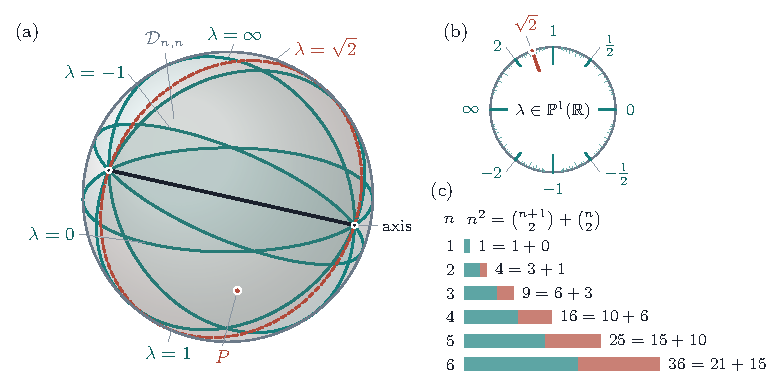
\includegraphics[width=0.80\textwidth]{fig_lagsweep}
\caption{The quaternionic loci of \Cref{prop:lagrangian}, drawn as a
pencil. Each admissible $\psi$ gives one leaf, an open piece of
$\mathrm{LG}(n,V_{+},\omega_{\psi})$ of dimension $n(n+1)/2$. As $\psi$
varies over the reals the leaves through a common axis form a continuous
family and sweep out $\cD_{n,n}$. The two heavy leaves are those with $\psi$
rational, and only such leaves are quaternionic loci of abelian varieties.
The drawing is faithful to the continuity of the family and to the
discreteness of its rational members, but not to dimensions: in the family
the leaves have dimension $n(n+1)/2$ inside $n^{2}$, hence codimension
$n(n-1)/2$, which vanishes only at $n=1$ (at $n=2$ the leaves are divisors,
\Cref{rem:ntwo}), and $\psi$ ranges over a real variety rather than an
interval.}
\label{fig:lagsweep}
\end{figure}

\begin{remark}[Real and rational quaternionic loci]%
\label{rem:onlyrational}
Fix a point $P$ of $\cD_{n,n}$, and let $\psi_{0}$ be left multiplication by
$j$ at a point $P_{0}$ given by \Cref{thm:quatweil}(iii). The group
$\SU(V,H)(\RR)$ acts transitively on the bounded symmetric domain $\cD_{n,n}$
of \Cref{prop:weildomain}, so $P=gP_{0}$ for some real $g$; since $g$ is
$K$-linear and preserves $H$, hence $E$, the map
$\psi=g\psi_{0}g^{-1}$ is $K$-semilinear, invertible and Rosati-symmetric,
satisfies $\psi^{2}=b$, and preserves the Hodge structure at $P$. It
satisfies every condition of \Cref{prop:lagrangian} except rationality, and
$P$ lies on its locus. So the quaternionic loci, taken over the \emph{real}
$\psi$, cover $\cD_{n,n}$; they cover it with room to spare, since each has
dimension $n(n+1)/2$ and they are parametrised by a positive-dimensional
family. What prevents the quaternionic loci of abelian varieties from
covering it is that $\psi$ must lie in $\End^{0}(A)$, hence be rational, and
the rational $\psi$ form a countable set.

This is the dichotomy of \Cref{cor:allornothing} in its simplest form. The
obstruction is the countability of a set of parameters inside an uncountable
one, and it involves neither deformation theory nor positivity. What is
needed is a mechanism that produces, from one rational $\psi$, a family of
cycles representing $\omega$ over an open subset of $\cD_{n,n}$ rather than
over the locus of $\psi$ alone; by \Cref{cor:allornothing}, such a family
would answer \Cref{q:residual} in the affirmative.
\end{remark}

\subsection{Absolutely Hodge classes and the exact form}\label{ssec:exactform}

The algebraicity of a Hodge class is usually approached through an
intermediate property. A rational class of type $(p,p)$ on a smooth
projective variety $X$ over $\CC$ is \emph{absolutely Hodge} if, for every
automorphism $\sigma$ of $\CC$, the conjugate under $\sigma$ of its de Rham
component is the de Rham component of a rational class of type $(p,p)$ on the
conjugate variety $X^{\sigma}$. The implications
\begin{equation}\label{eq:threechain}
  \text{algebraic}
  \;\Longrightarrow\;
  \text{absolutely Hodge}
  \;\Longrightarrow\;
  \text{Hodge}
\end{equation}
are both elementary. The Hodge conjecture asserts the converse of their
composite. The converse of the second is the weaker statement, and Deligne
proved it for abelian varieties, so on abelian varieties the Hodge conjecture
is the converse of the first.

\begin{theorem}[Deligne \cite{Del82}]\label{thm:deligneAH}
Every Hodge class on a complex abelian variety is absolutely Hodge. Moreover,
\emph{Principle B}: if $\pi\colon\cX\to S$ is smooth projective over a
connected smooth base, and $\alpha$ is a flat section of $R^{2p}\pi_{*}\QQ(p)$
that is Hodge at every point of $S$ and absolutely Hodge at one point, then it
is absolutely Hodge at every point.
\end{theorem}

Together with \Cref{thm:residual} and \Cref{thm:everyfamily}, this locates
the remaining problem.

\begin{corollary}[Reduction to an absolutely Hodge class]\label{cor:exactform}
Let $\pi\colon\cA\to\cD_{n,n}$ and $\omega$ be as in \Cref{setup:family}. Then
$\omega_{s}$ is absolutely Hodge for every $s$, and the following are
equivalent:
\begin{enumerate}[label=\textup{(\roman*)},nosep]
\item the Hodge conjecture holds, in every degree, for every abelian
  $2n$-fold of $(K,-1,n)$-Weil type with $\Hg(A)=\SU(V,H)$;
\item the absolutely Hodge class $\omega_{s}$ is algebraic for every $s$.
\end{enumerate}
This holds for every $K$, every $n$ and every discriminant.
\end{corollary}

\begin{proof}
The first assertion is \Cref{thm:deligneAH}. It also follows from Principle B
together with \Cref{thm:everyfamily}, which supplies a point of $\cD_{n,n}$ at
which $\omega$ is algebraic and hence absolutely Hodge, and with the
connectedness of $\cD_{n,n}$ from \Cref{prop:weildomain}.

That (ii) implies (i) is \Cref{thm:residual}(a). Conversely, the Hodge group
of $A_{s}$ is $\SU(V,H)$ for $s$ outside a countable union of proper closed
analytic subsets of $\cD_{n,n}$, by Weil's theorem \cite{Weil77} recalled
before \Cref{thm:hdgcount}. Under (i) the class $\omega_{s}$ is algebraic at
all such $s$, so the set $\Sigma$ of points at which it is algebraic is not
meagre, and \Cref{cor:allornothing} gives $\Sigma=\cD_{n,n}$, which is (ii).
\end{proof}

\section{The algebraic locus and the propagation criteria}\label{sec:propagation}

The results of \Cref{sec:basepoints} are pointwise: a class, a criterion and
a cycle at a point, and in \Cref{cor:exactform} an implication to be proved
at every point. This section studies the set of points at which the Weil class
is algebraic. Properness of the Hilbert scheme makes it a countable union of
closed subvarieties (\Cref{thm:closedlocus}), and rational isogenies make it
dense (\Cref{prop:densealg}); together these turn the propagation question
into a dichotomy (\Cref{cor:allornothing}). Two criteria for propagation
follow, a bound along one orbit (\Cref{thm:degreebound}) and a rank at one
point (\Cref{thm:semiregclosure}). We treat the bound first, together with
the transport of cycles along isogenies, which decides one of its two
readings, and with the limits of representatives built from products of
divisors; the rest of the section is devoted to the rank.

\subsection{The algebraic locus}
\label{ssec:properness}

\Cref{q:residual} is a question about the set
\[
  \Sigma \;=\; \bigl\{\,s\in\cD_{n,n} \;:\;
    \omega_{s}\ \text{is algebraic on}\ A_{s}\,\bigr\}.
\]
This set is restricted in shape, and the restriction changes the form
of the remaining problem: instead of a class to construct at every point, one
is left with a bound to prove along one orbit, or a rank to compute at one
point. The reason is that the Hilbert scheme is proper, so each piece of
$\Sigma$ cut out by bounded data is Zariski closed. The mechanism is standard:
the locus where a fixed Hodge class becomes algebraic is a countable union of
closed subvarieties, the companion of the statement that the Hodge locus
itself is one (see \cite[Chapter~5]{Voi03} and, in the form used in
\Cref{thm:cdk}, \cite{CDK95}). What is particular to the present situation is
that the class is determined by \Cref{thm:hdgcount} and written out by
\Cref{thm:explicitgens}, that its algebraic locus is nonempty in every family
by \Cref{thm:everyfamily}, and that the group acting on the family is known.

\begin{setupenv}[The quotient and the universal family]\label{setup:shimura}
Keep \Cref{setup:family}. Fix an integer $N\ge3$ and let $\Gamma$ be the
subgroup of $\SU(V,H)(\QQ)$ preserving the lattice $L\subset V$ used to build
the family and acting trivially on $L/NL$. Write
\[
  p\colon\cD_{n,n}\longrightarrow\cS=\Gamma\backslash\cD_{n,n} .
\]
Since $N\ge3$ the group $\Gamma$ is torsion-free, so it acts freely on
$\cD_{n,n}$, and by Baily and Borel \cite{BB66} the quotient $\cS$ is a smooth
quasi-projective complex variety; it is irreducible because $\cD_{n,n}$ is
connected. The level structure rigidifies, so $\cS$ carries a universal family
\[
  f\colon\cA\longrightarrow\cS,
\]
and the relative polarisation $3\eta$ is relatively very ample, which fixes a
relative projective embedding and hence a notion of degree in the fibres.
Write $G=\SU(V,H)$, an algebraic group over $\QQ$, so that
$G(\RR)$ acts transitively on $\cD_{n,n}$ and $\Gamma\subset G(\QQ)$.
\end{setupenv}

We record two facts that are used repeatedly below.

\begin{lemma}[The section descends]\label{lem:omegadescends}
The section $\omega$ of \Cref{setup:family} is $\Gamma$-invariant, hence
descends to a flat section of $R^{2n}f_{*}\QQ$ over $\cS$ that is of type
$(n,n)$ at every point.
\end{lemma}

\begin{proof}
The Weil line is $\HW=\bigwedge^{2n}_{K}V$, and an element of $\SU(V,H)$ is by
definition a $K$-linear automorphism of $V$ of $K$-determinant $1$. Its action
on the top $K$-exterior power is multiplication by that determinant, so
$\Gamma$ acts trivially on $\HW$ and in particular fixes $\omega$. Flatness is
then immediate, and the Hodge type at every point is
\Cref{prop:weilline}(ii).
\end{proof}

\begin{lemma}[One component is enough]\label{lem:onecomponent}
Let $(A,\iota,\eta)$ be of $(K,-1,n)$-Weil type with
$\iota(\cO_{K})\subseteq\End(A)$, and let $\HW\subset H^{2n}(A,\QQ)$ be its
Weil line. If one nonzero element of $\HW$ is algebraic, every element of
$\HW$ is algebraic.
\end{lemma}

\begin{proof}
Among the elements $\tau_{m}=m+\sqrt{-d}$ of $\cO_{K}$ with $1\le m\le7$ the
ratios $\tau_{m}/\bbar{\tau}_{m}$ are pairwise distinct, since
$\tau_{m}\bbar{\tau}_{m'}$ is rational only when $m=m'$. The group of roots of
unity in an imaginary quadratic field has order $2$, $4$ or $6$, so some $m$
in that range has $\tau=\tau_{m}$ with $\tau/\bbar\tau$ not a root of unity,
and then $\tau^{2n}\ne\bbar{\tau}^{2n}$, that is $\tau^{2n}\notin\QQ$, for
every $n\ge1$. A range is needed, since the witness $m=1$ fails for two
fields: for $d=1$ the ratio attached to $1+\sqrt{-1}$ is a primitive fourth
root of unity, and for $d=3$ the ratio attached to $1+\sqrt{-3}$ is a
primitive cube root of unity, so $(1+\sqrt{-d})^{2n}$ is rational when $d=1$
and $n$ is even, and when $d=3$ and $3\mid n$.

Since $\tau\in\cO_{K}$, the element $\iota(\tau)$ is an endomorphism of $A$,
so $\iota(\tau)^{*}$ on $H^{2n}(A,\QQ)$ is induced by the graph
correspondence and therefore carries algebraic classes to algebraic classes.
On $H^{1}$ it is multiplication by $\tau$, so on
$\bigwedge^{2n}_{K}V$ it is multiplication by $\tau^{2n}$. As
$\tau^{2n}\notin\QQ$ and $\HW$ is a one-dimensional $K$-vector space, the pair
$w,\;\tau^{2n}w$ is a $\QQ$-basis of $\HW$ for every $w\ne0$. Explicitly, fix
a $K$-basis $w_{0}$ of $\HW$ and write $\tau^{2n}=a+b\sqrt{-d}$, so that
$b\ne0$, and $w=(w_{1}+w_{2}\sqrt{-d})\,w_{0}$; the determinant of the pair
$w,\tau^{2n}w$ in the $\QQ$-basis $w_{0},\sqrt{-d}\,w_{0}$ is
$b(w_{1}^{2}+dw_{2}^{2})$, which is nonzero when $w\ne0$. If $w$ is
algebraic then so is $\iota(\tau)^{*}w=\tau^{2n}w$, and the two together span.
\end{proof}

\Cref{lem:onecomponent} writes out the last step of the proof of
\Cref{cor:whatisleft}, where the witness $\tau$ has to be chosen.

\begin{theorem}[The algebraic locus is a countable union of closed
subvarieties]\label{thm:closedlocus}
Keep \Cref{setup:shimura}. For a finite tuple $\underline{P}=(P_{1},\dots
,P_{m})$ of Hilbert polynomials of degree $n$ and a tuple
$\underline{q}\in\QQ^{m}$ put
\begin{align*}
  \cH_{\underline{P}}
  &\;=\;
  \Hilb^{P_{1}}(\cA/\cS)\times_{\cS}\cdots\times_{\cS}\Hilb^{P_{m}}(\cA/\cS),
  \\[2pt]
  \Sigma_{\underline{P},\underline{q}}
  &\;=\;
  \mathrm{pr}\Bigl(\bigl\{\,\underline{Z}\in\cH_{\underline{P}}
    \;:\;\textstyle\sum_{i}q_{i}[Z_{i}]=\omega\,\bigr\}\Bigr)
  \;\subseteq\;\cS .
\end{align*}
Then each $\Sigma_{\underline{P},\underline{q}}$ is Zariski closed in
$\cS$, and
\[
  p^{-1}\Bigl(\,\bigcup_{\underline{P},\underline{q}}
    \Sigma_{\underline{P},\underline{q}}\Bigr)\;=\;\Sigma ,
\]
the union running over a countable index set.
\end{theorem}

\begin{proof}
Each $\Hilb^{P_{i}}(\cA/\cS)$ is projective over $\cS$ by Grothendieck's
construction of the Hilbert scheme \cite{Gro61}, so the fibre product
$\cH_{\underline{P}}$ is
projective over $\cS$, and being of finite type it has finitely many connected
components.

Fix a connected component $T$, replace it by its reduction, which changes
neither the underlying space nor any cohomology group, and let
$\cZ_{i}\subset\cA\times_{\cS}T$ be the pullback of the $i$-th universal
subscheme. It is flat over $T$ and its fibres have Hilbert polynomial $P_{i}$
of degree $n$, so the associated $n$-cycles, the top-dimensional components
counted with their multiplicities, are the fibres of a cycle on
$\cA\times_{\cS}T$ whose class restricts on the fibre over $t$ to $[Z_{i,t}]$.
Restriction of a global class to the fibres of a topologically
locally trivial family is a flat section of the local system, so
$t\mapsto\sum_{i}q_{i}[Z_{i,t}]$ is flat on $T$; and $\omega$ is flat on $\cS$
by \Cref{lem:omegadescends}, hence flat after pullback. Two flat sections of a
local system over a connected base agree everywhere as soon as they agree at
one point, so the locus where they agree is a union of connected components of
$\cH_{\underline{P}}$. That locus is therefore itself projective over $\cS$,
and the image of a proper morphism is Zariski closed.

For the equality of sets, let $s\in\Sigma$. Then
$\omega_{s}=\sum_{i}q_{i}[Z_{i}]$ for finitely many closed integral subschemes
$Z_{i}\subset A_{s}$ of dimension $n$ and rationals $q_{i}$; taking
$P_{i}$ to be the Hilbert polynomial of $Z_{i}$ puts $p(s)$ in
$\Sigma_{\underline{P},\underline{q}}$. The converse holds because the class
of the $n$-cycle of a closed subscheme of dimension $n$ is algebraic. The
index set is countable, since a Hilbert polynomial is determined by its
finitely many integer coordinates in the binomial basis, and $\QQ$ is
countable.
\end{proof}

The bound on the Hilbert polynomials cannot be dropped: without it one takes
the image of an infinite disjoint union, and an infinite union of closed sets
need be neither closed nor constructible, and the dichotomy below is what
can be said of $\Sigma$ itself. Tuples are needed because a rational cycle is a rational combination
of several integral ones, which may have different Hilbert polynomials. The
relative Chow variety of effective $n$-cycles of bounded degree would serve
equally well, with the same proof, since only properness over the base and
local constancy of the cycle class are used.

\begin{corollary}[The dichotomy]\label{cor:allornothing}
Exactly one of the following holds.
\begin{enumerate}[label=\textup{(\alph*)},nosep]
\item $\Sigma=\cD_{n,n}$, and the Hodge conjecture holds in every degree for
  every abelian $2n$-fold of $(K,-1,n)$-Weil type with $\Hg(A)=\SU(V,H)$ in
  the family.
\item $\Sigma$ has empty interior in the analytic topology. Its complement is
  then a dense $G_{\delta}$, so $\omega_{s}$ fails to be algebraic for every
  $s$ outside a meagre set, and the Hodge conjecture fails.
\end{enumerate}
In particular, if $\omega_{s}$ is algebraic for all $s$ in some nonempty open
subset of $\cD_{n,n}$, then it is algebraic for all $s$.
\end{corollary}

\begin{proof}
Suppose $\Sigma$ contains a nonempty open set; then so does its image in
$\cS$, and we may pick a nonempty connected open $U\subseteq\cS$ contained in
that image. By \Cref{thm:closedlocus} the countably many sets
$\Sigma_{\underline{P},\underline{q}}\cap U$ are closed in $U$ and cover it.
A connected complex manifold is a Baire space, so one of them has nonempty
interior in $U$. A Zariski closed subset of the irreducible variety $\cS$
either is all of $\cS$ or is a proper closed subvariety, and a proper closed
subvariety of a connected complex manifold has empty interior. Hence that
$\Sigma_{\underline{P},\underline{q}}$ is all of $\cS$, so $\Sigma=\cD_{n,n}$
and (a) holds by \Cref{thm:residual}(a). If $\Sigma$ has empty interior, its
complement is the intersection of the countably many dense open sets
$\cD_{n,n}\setminus p^{-1}(\Sigma_{\underline{P},\underline{q}})$, and Baire
again gives that this intersection is dense. At each of its points
$\omega_{s}$ is a Hodge class by \Cref{lem:omegadescends} and is not
algebraic, so the Hodge conjecture fails there.
\end{proof}

\Cref{fig:properness} draws the two cases.

\begin{figure}[htbp]
\centering
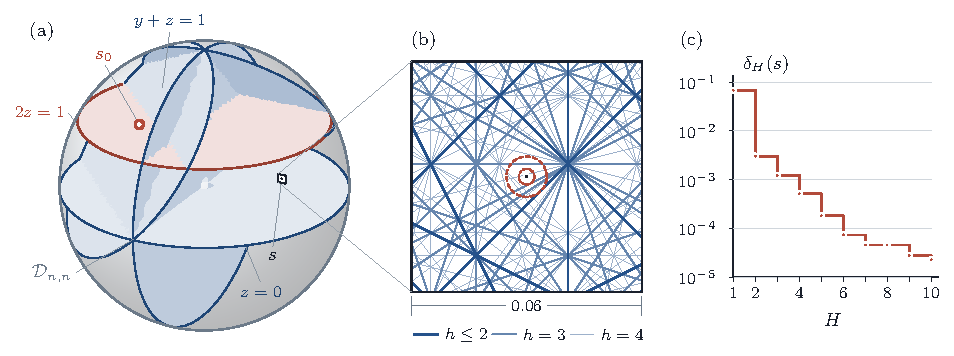
\includegraphics[width=0.88\textwidth]{fig_properness}
\caption{The dichotomy of \Cref{cor:allornothing}. Each stratum
$\Sigma_{\underline{P},\underline{q}}$ is Zariski closed by
\Cref{thm:closedlocus}, and there are countably many of them; the base point
$s_{0}$ of \Cref{thm:everyfamily} lies on one. By \Cref{prop:densealg} the
union of the strata is dense, so every neighbourhood of a point $s$ lying
off all of them meets infinitely many strata. The conjecture for the family
is the assertion that no such $s$ exists, and by \Cref{cor:allornothing} it
is enough that one stratum has nonempty interior.}
\label{fig:properness}
\end{figure}

\begin{lemma}[Invariance under rational isogenies]\label{lem:Ginvariance}
$\Sigma$ is stable under the action of $G(\QQ)$ on $\cD_{n,n}$.
\end{lemma}

\begin{proof}
A point of $\cD_{n,n}$ is a complex structure $J$ on $V_{\RR}$ compatible with
$H$, and $g\in G(\QQ)$ carries $J$ to $gJg^{-1}$. The map $g$ is then
$\QQ$-rational and $\CC$-linear from $(V_{\RR},J)$ to $(V_{\RR},gJg^{-1})$, so
after clearing denominators it induces an isogeny $A_{J}\to A_{gJ}$, whose
graph is an algebraic correspondence. Algebraicity of a rational cohomology
class is preserved by such a correspondence and by its transpose. Finally $g$
lies in $\SU(V,H)$, so by the computation in \Cref{lem:omegadescends} it fixes
the Weil line pointwise; the correspondence therefore carries $\omega_{J}$ to
a nonzero rational multiple of $\omega_{gJ}$, and $\omega_{gJ}$ is algebraic
when $\omega_{J}$ is.
\end{proof}

Two density statements should be distinguished. For a class that does not
remain of Hodge type over the whole family, the locus where it is of Hodge
type is a countable union of proper closed subvarieties, each algebraic by
\Cref{thm:cdk}, and density there concerns the distribution of special
points. For the class $\omega$ of \Cref{setup:family} the Hodge locus is the
whole family by \Cref{prop:weilline}(ii), so \Cref{thm:cdk} gives no
information, and the set that carries information is the algebraic locus. The
next proposition concerns that set, and its proof uses no Hodge theory: the
algebraic locus is a union of orbits of a group whose rational points are
dense in its real points.

\begin{proposition}[The algebraic locus is dense]\label{prop:densealg}
Let $n\ge2$. Then $\Sigma$ is dense in $\cD_{n,n}$ in the analytic topology,
and its image in $\cS$ is dense.
\end{proposition}

\begin{proof}
The hermitian form $H$ has rank $2n\ge4$ over $K$ and signature $(n,n)$, so it
is isotropic over $\RR$; over every $\QQ_{p}$ a hermitian form of rank at
least three over a quadratic extension is isotropic; and hermitian forms over
an imaginary quadratic field satisfy the Hasse principle
\cite[Ch.~10, \S 6]{Sch85}. So $H$ is isotropic over $\QQ$ and $G$ is
$\QQ$-isotropic. The group $G=\SU(V,H)$ is simply connected and almost
$\QQ$-simple, so by Platonov's theorem $G(\QQ)$ is generated by the rational
points of the unipotent radicals of its proper parabolic $\QQ$-subgroups
\cite[Thm.~7.6 and \S 7.2]{PR94}. For a unipotent group $U$ over $\QQ$ the
exponential identifies $U(\QQ)$ with a $\QQ$-vector space inside the
corresponding $\RR$-vector space $U(\RR)$, so $U(\QQ)$ is dense in $U(\RR)$.
The closure of $G(\QQ)$ in $G(\RR)$ therefore contains $U(\RR)$ for every such
$U$, and those generate the identity component $G(\RR)^{+}$, which acts
transitively on $\cD_{n,n}$. Hence every $G(\QQ)$-orbit in $\cD_{n,n}$ is
dense.

By \Cref{thm:everyfamily} the set $\Sigma$ is nonempty, and by
\Cref{lem:Ginvariance} it is $G(\QQ)$-stable, so it contains a dense orbit.
The projection $p$ is continuous and surjective, so the image is dense.
\end{proof}

In particular, if case (b) of \Cref{cor:allornothing} occurs, then $\Sigma$
and its complement are both dense, and the two sets are distinguished by
Baire category and not by position.

\begin{corollary}[A Baire category criterion]\label{cor:meagre}
Let $n\ge2$. The Hodge conjecture holds for every abelian $2n$-fold of
$(K,-1,n)$-Weil type with $\Hg(A)=\SU(V,H)$ in the family of
\Cref{setup:family} if and only if $\Sigma$ is non-meagre in $\cD_{n,n}$, and
if and only if $\Sigma$ has nonempty interior.
\end{corollary}

\begin{proof}
If $\Sigma=\cD_{n,n}$, both conditions hold, and so does the conjecture, by
\Cref{thm:residual}(a). Otherwise case (b) of \Cref{cor:allornothing} holds,
so $\Sigma$ has empty interior; it is then the countable union of the closed
sets $p^{-1}(\Sigma_{\underline{P},\underline{q}})$, each with empty interior,
and so it is meagre. The points $s$ with $\Hg(A_{s})=\SU(V,H)$ form the
complement of a countable union of proper closed analytic subsets of $\cD_{n,n}$, by
Weil's theorem \cite{Weil77} recalled before \Cref{thm:hdgcount}, so by Baire
they are not all contained in the meagre set $\Sigma$. At a point of this
kind outside $\Sigma$ the Hodge conjecture fails for $A_{s}$.
\end{proof}

\subsection{The first criterion: a bound along one orbit}

The proof of \Cref{prop:densealg} produces the dense algebraic locus by
transporting one cycle along rational isogenies, and an isogeny multiplies
degrees. The dense set so obtained is therefore stratified by unbounded data,
and this is what prevents \Cref{cor:allornothing} from applying to it. A bound
on the data along one orbit removes the difficulty.

\begin{theorem}[A bound along the orbit closes the family]\label{thm:degreebound}
Let $n\ge2$ and let $s_{0}\in\Sigma$ be one of the base points supplied by
\Cref{thm:everyfamily}. Suppose that there is a finite set $\mathcal{T}$ of pairs
$(\underline{P},\underline{q})$ such that for every $g\in G(\QQ)$ the class
$\omega_{g\cdot s_{0}}$ is represented by some cycle whose Hilbert data lies
in $\mathcal{T}$. Then $\Sigma=\cD_{n,n}$, and the Hodge conjecture holds in every
degree for every abelian $2n$-fold of $(K,-1,n)$-Weil type with
$\Hg(A)=\SU(V,H)$ in that family.
\end{theorem}

\begin{proof}
The orbit $G(\QQ)\cdot s_{0}$ is dense by the proof of \Cref{prop:densealg},
and by hypothesis it is the union of the finitely many sets
$G(\QQ)\cdot s_{0}\cap p^{-1}(\Sigma_{\underline{P},\underline{q}})$ with
$(\underline{P},\underline{q})\in\mathcal{T}$. The union of the finitely
many closed sets $p^{-1}(\Sigma_{\underline{P},\underline{q}})$,
$(\underline{P},\underline{q})\in\mathcal{T}$, therefore contains a dense set,
and so it is all of $\cD_{n,n}$; in particular $\Sigma=\cD_{n,n}$. In fact one
of these sets is already all of $\cS$: each
$\Sigma_{\underline{P},\underline{q}}$ is Zariski closed in the irreducible
variety $\cS$, hence either equal to $\cS$ or nowhere dense, and a finite
union of nowhere dense sets is nowhere dense. The Hodge conjecture for the
family follows by \Cref{thm:residual}(a).
\end{proof}

\begin{remark}[Choice of the representing cycle]\label{rem:chosencycle}
We call the hypothesis of \Cref{thm:degreebound} the bounded criterion
\textup{(P1)}; \Cref{rem:tworemain} lists it beside the rank criterion
\textup{(P2)} of \Cref{thm:semiregclosure}. It quantifies over representing
cycles at each point of the orbit and asks only that, at each point, one of
them have bounded complexity. A stronger hypothesis would fix the cycle,
taking at $g\cdot s_{0}$ the transport of the cycle at $s_{0}$ along the
isogeny of \Cref{lem:Ginvariance}. \Cref{thm:p1forces} below shows that this
stronger form is never satisfied by a base cycle with a component of finite
stabiliser, since the transported data is then unbounded. The proof above
uses only the weaker hypothesis, which is what the covering argument needs.
\end{remark}

The hypothesis of \Cref{thm:degreebound} can be sharpened by locating the
part of the Hilbert data that is at issue. The leading coefficient is not.

\begin{proposition}[The leading coefficient is constant on the orbit]
\label{prop:leadingconstant}
Let $s_{0}\in\Sigma$ and $g\in G(\QQ)$, and let $\omega_{s}$ denote the Weil
class at $s$ and $\eta$ the polarisation class. Then
\[
  \int_{A_{g\cdot s_{0}}}\omega_{g\cdot s_{0}}\cdot\frac{\eta^{n}}{n!}
  \;=\;\int_{A_{s_{0}}}\omega_{s_{0}}\cdot\frac{\eta^{n}}{n!},
\]
so the degree of the transported class with respect to the polarisation, which
is the leading coefficient of the Hilbert polynomial of any cycle
representing it, is the same at every point of the orbit.
\end{proposition}

\begin{proof}
By \Cref{lem:Ginvariance} the correspondence transporting the class is induced
by a $\QQ$-rational map $g\in\SU(V,H)$. It preserves the hermitian form and
hence the polarisation class, it fixes the Weil line pointwise by
\Cref{lem:omegadescends}, and its determinant over $\QQ$ is
$\Nm_{K/\QQ}(\det_{K}g)=1$, so it acts trivially on the top exterior power of
$V^{\vee}$, in which both integrals are evaluated. The two integrals are
therefore equal. The identification of the number with the leading
coefficient is Hirzebruch--Riemann--Roch on $A$, whose Todd class is $1$ (for
the embedding by $3\eta$ of \Cref{setup:shimura} the leading coefficient is
$3^{n}$ times the number); the remaining coefficients involve the structure
sheaf of the cycle and not only its class.
\end{proof}

\begin{remark}[The source of unboundedness]
\label{rem:whereunbounded}
Write a representing cycle at a point of the orbit, the transported cycle or
any other, as a difference $\xi^{+}-\xi^{-}$ of effective cycles. By
\Cref{prop:leadingconstant} the difference of their degrees is constant along
the orbit, and by the boundedness of effective cycles of bounded degree in
the fibres of the polarised family $f\colon\cA\to\cS$, if $\deg\xi^{+}$ were
bounded along the orbit then only finitely many tuples
$(\underline{P},\underline{q})$ could occur and \Cref{thm:degreebound} would
apply. So the hypothesis of that theorem is equivalent to a bound on the
effective part alone.

This bound is not automatic, and the mechanism that threatens it can be seen
directly. The transport at $g$ is by the isogeny obtained from $g$ by
clearing denominators; if $g$ has denominator $m$ on the reference lattice,
which has rank $4n$, the isogeny has degree $m^{4n}$ (\Cref{lem:transport}
below), and pushing a cycle forward along it multiplies its multiplicities
and degrees by powers of $m$ (\Cref{lem:multiplicity}). Elements of $G(\QQ)$ of bounded denominator form a discrete subset of
$G(\RR)$, so along a dense orbit the denominators, and with them the isogeny
degrees, are unbounded. What \Cref{thm:degreebound} asks is that the cycles
nevertheless simplify: that at each point of the orbit the class $\omega$,
whose degree has not changed, admits an effective representation no more
complicated than before. For the transported cycle itself the answer is
negative as soon as a component of the base cycle has finite stabiliser
(\Cref{thm:p1forces} below), and for a cycle chosen at each point the bound
is equivalent to the conclusion (\Cref{thm:p1equivalent}). The present remark
shows only that the question reduces from the whole Hilbert datum to the
degree of the effective part, and that the part of the datum determined by
cohomology is constant.
\end{remark}

\subsection{Transport along isogenies}

The mechanism of \Cref{rem:whereunbounded} can be made explicit, and doing
so settles one of the two readings of \textup{(P1)}: the reading in
which the cycle at $s_{0}$ is transported along the orbit rather than chosen
afresh at each point. Write $\Lambda$ for the reference lattice, of rank $4n$
over $\ZZ$, and $E$ for the alternating form of the polarisation, so that a
point $s$ of $\cD_{n,n}$ is a complex structure on $\Lambda\otimes\RR$ and
$A_{s}=(\Lambda\otimes\RR)/\Lambda$. Throughout, $\dim A_{s}=2n$, and a
component of a cycle representing $\omega_{s}$ has dimension $n$.

\begin{lemma}[The transport in coordinates]\label{lem:transport}
Let $g\in G(\QQ)$ and let $c=c(g)$ be the least positive integer with
$cg\Lambda\subseteq\Lambda$. Then $\varphi_{g}:=cg$ induces an isogeny
$A_{s_{0}}\to A_{g\cdot s_{0}}$ with
\begin{enumerate}[label=\textup{(\roman*)},nosep,leftmargin=2.6em]
\item $\deg\varphi_{g}=c^{4n}$;
\item $\varphi_{g}^{*}\eta_{g\cdot s_{0}}=c^{2}\eta_{s_{0}}$ and
  $\varphi_{g}^{*}\omega_{g\cdot s_{0}}=c^{2n}\omega_{s_{0}}$;
\item the transported cycle representing $\omega_{g\cdot s_{0}}$ is
  $c^{-2n}\,\varphi_{g*}(Z)$, where $Z$ represents $\omega_{s_{0}}$.
\end{enumerate}
Moreover $\sup_{g\in G(\QQ)}c(g)=\infty$.
\end{lemma}

\begin{proof}
(i) The index of $cg\Lambda$ in $\Lambda$ is $|\det_{\QQ}(cg)|
=c^{4n}|\det_{\QQ}g|$, and $\det_{\QQ}g=\Nm_{K/\QQ}(\det_{K}g)=1$ for
$g\in\SU(V,H)$.

(ii) $g$ preserves $E$, so $(cg)^{*}E=c^{2}E$, which is the first identity.
On $H^{2n}=\bigwedge^{2n}(\Lambda^{\vee}\otimes\QQ)$ the map
$\varphi_{g}^{*}$ is $c^{2n}\bigwedge^{2n}g^{\vee}$, and $g\in\SU(V,H)$ fixes
the Weil line pointwise by \Cref{lem:omegadescends}.

(iii) $\varphi_{g*}\varphi_{g}^{*}=\deg\varphi_{g}$, so
$\omega_{g\cdot s_{0}}=(\deg\varphi_{g})^{-1}\varphi_{g*}
\varphi_{g}^{*}\omega_{g\cdot s_{0}}
=c^{-4n}\,c^{2n}\varphi_{g*}\omega_{s_{0}}=c^{-2n}\varphi_{g*}\omega_{s_{0}}$
by (i) and (ii).

For the last sentence, suppose that $c(g)\le C$ for every $g\in G(\QQ)$.
Then $(C!)\,g\Lambda\subseteq\Lambda$ for every $g$, so $G(\QQ)$ lies in the
discrete subset $(C!)^{-1}\End_{\ZZ}(\Lambda)$ of $\End(\Lambda\otimes\RR)$.
But by the proof of \Cref{prop:densealg} the closure of $G(\QQ)$ in $G(\RR)$
contains $G(\RR)^{+}$, a Lie group of positive dimension, which is a
contradiction.
\end{proof}

\begin{lemma}[Push-forward along an isogeny]
\label{lem:multiplicity}
Let $\varphi\colon A\to A'$ be an isogeny of abelian varieties and $Z\subseteq A$
an integral closed subvariety. Put
$G(Z)=\{x\in A:Z+x=Z\}$, a closed algebraic subgroup. Then
\[
  \varphi_{*}[Z]=m\,[\varphi(Z)],\qquad
  m=\bigl|\ker\varphi\cap G(Z)\bigr| .
\]
If moreover $\dim Z=n$ and $\varphi^{*}\eta'=c^{2}\eta$, then
\[
  \deg_{\eta'}\varphi(Z)=\frac{c^{2n}}{m}\,\deg_{\eta}Z .
\]
\end{lemma}

\begin{proof}
The map $\varphi|_{Z}\colon Z\to\varphi(Z)$ is finite and surjective, and its
degree $m$ is the number of points of a general fibre. For $z\in Z$ the fibre
through $z$ is $Z\cap(z+\ker\varphi)$, which as a set of translations is
$\{t\in\ker\varphi:z+t\in Z\}$. For a fixed $t$ the locus
$\{z\in Z:z+t\in Z\}=Z\cap(Z-t)$ is all of $Z$ when $t\in G(Z)$ and a proper
closed subset otherwise; since $\ker\varphi$ is finite, a general $z$ avoids
the finitely many proper subsets, and there
$\{t\in\ker\varphi:z+t\in Z\}=\ker\varphi\cap G(Z)$. This is the first
identity, and $\varphi_{*}[Z]=m[\varphi(Z)]$ by the definition of the
push-forward of cycles.

For the degree, the projection formula gives
\[
  m\deg_{\eta'}\varphi(Z)=\int\varphi_{*}[Z]\cdot\frac{\eta'^{n}}{n!}
  =\int[Z]\cdot\frac{(\varphi^{*}\eta')^{n}}{n!}
  =c^{2n}\int[Z]\cdot\frac{\eta^{n}}{n!}=c^{2n}\deg_{\eta}Z .
\]
\end{proof}

For example, for multiplication by $c$ on an abelian variety of dimension $2n$,
an abelian subvariety $Z$ of dimension $n$ has $G(Z)=Z$, so $m=|Z[c]|=c^{2n}$
and $\deg\varphi(Z)=\deg Z$, while a $Z$ whose stabiliser meets $A[c]$
trivially has $m=1$ and $\deg\varphi(Z)=c^{2n}\deg Z$.

\begin{theorem}[The transported cycle]\label{thm:p1forces}
Let $s_{0}\in\Sigma$ and let $Z=\sum_{i}q_{i}Z_{i}$, with $q_{i}\ne0$ and the
$Z_{i}$ integral of dimension $n$, represent $\omega_{s_{0}}$.
\begin{enumerate}[label=\textup{(\roman*)},leftmargin=2.6em,itemsep=2pt]
\item For $g\in G(\QQ)$ the transported cycle is
  $\sum_{i}c(g)^{-2n}m_{i}(g)\,q_{i}\,[\varphi_{g}(Z_{i})]$ with
  $m_{i}(g)=|\ker\varphi_{g}\cap G(Z_{i})|$, and the $i$-th component has
  degree $c(g)^{2n}\deg_{\eta}(Z_{i})/m_{i}(g)$.
\item If some $Z_{i}$ has finite stabiliser $G(Z_{i})$, then
  $\deg\varphi_{g}(Z_{i})\ge c(g)^{2n}\deg_{\eta}(Z_{i})/|G(Z_{i})|$, which is
  unbounded on $G(\QQ)$. The Hilbert data of the transported cycle then takes
  infinitely many values, and the hypothesis of \Cref{thm:degreebound} in the
  form that fixes the transported cycle is not satisfied by $Z$.
\item Consequently, a base cycle for which the transported data is bounded
  must have every component of positive-dimensional stabiliser, that is, every
  $Z_{i}$ must be stable under translation by a positive-dimensional abelian
  subvariety of $A_{s_{0}}$.
\end{enumerate}
\end{theorem}

\begin{proof}
(i) is \Cref{lem:transport}(iii) and \Cref{lem:multiplicity}.

(ii) $\ker\varphi_{g}\cap G(Z_{i})\subseteq G(Z_{i})$, so
$m_{i}(g)\le|G(Z_{i})|$, a constant; the displayed bound is (i), and $c(g)$ is
unbounded by \Cref{lem:transport}. Distinct degrees of the components give
distinct Hilbert polynomials, so the data takes infinitely many values.

(iii) is the contrapositive of (ii), together with the fact that an algebraic
subgroup of positive dimension in an abelian variety has an abelian subvariety
of positive dimension as its identity component.
\end{proof}

\begin{remark}[The two readings of \textup{(P1)}]\label{rem:p1meaning}
Three points should be kept apart.

First, \textup{(P1)} has two readings, and \Cref{thm:p1forces} settles one of
them. Read with the cycle fixed at $s_{0}$ and transported, it fails for every
base cycle written down in this paper: those cycles are intersections of
divisors, and an intersection of $n$ divisors on an abelian $2n$-fold has
finite stabiliser unless the divisors are pulled back from a quotient, which
the ones here are not. Read with the cycle chosen afresh at each point of the
orbit, which is the form of the hypothesis of \Cref{thm:degreebound}, it is
not affected by \Cref{thm:p1forces}.

Second, the difference between the two readings is the content of
\Cref{lem:multiplicity}. The class $\omega_{g\cdot s_{0}}$ has constant degree
along the orbit, by \Cref{prop:leadingconstant}; what grows is the complexity
of the particular representative that the transport produces, because the
isogeny spreads each component out by the factor $c^{2n}/m_{i}$. When a
component of the base cycle has finite stabiliser, the transport does not
produce a representative of bounded complexity, whether or not one exists.

Third, an approach to \textup{(P1)} must either produce a base cycle supported
on subvarieties with positive-dimensional stabiliser, a strong requirement for
a Weil class, or abandon the transport and bound instead the minimal
complexity of a representative, which is a statement about the Chow variety of
the family and not about any one cycle. Neither is achieved here.
\end{remark}

The bound on the minimal complexity of a representative is the hypothesis of
\Cref{thm:degreebound}, and it is the weakest hypothesis under which the
covering argument runs. The next theorem shows that it is equivalent to the
conclusion. Write $\mathbf{W}(K,n,\delta)$ for the statement that every
abelian $2n$-fold of $(K,-1,n)$-Weil type with discriminant $\delta$
(\Cref{def:disc}) has algebraic Weil classes, $\delta$ being the discriminant
of the family of \Cref{setup:family}.

\begin{theorem}[Equivalence of the bounded criterion]\label{thm:p1equivalent}
Let $n\ge2$, let $s_{0}\in\Sigma$ and keep \Cref{setup:family}. The following
are equivalent.
\begin{enumerate}[label=\textup{(\alph*)},leftmargin=2.6em,itemsep=2pt]
\item There is a finite set $\mathcal{T}$ of pairs
  $(\underline{P},\underline{q})$ such that at every point of the orbit
  $G(\QQ)\cdot s_{0}$ the class $\omega$ is represented by a cycle whose
  Hilbert data lies in $\mathcal{T}$; that is, \textup{(P1)} holds at
  $s_{0}$.
\item There is a single pair $(\underline{P},\underline{q})$ such that at
  every point of $\cD_{n,n}$, not merely of the orbit, the class $\omega$ is
  represented by a cycle with that datum.
\item $\Sigma=\cD_{n,n}$.
\item $\mathbf{W}(K,n,\delta)$ holds, that is, the Weil classes are algebraic
  on every member of the family.
\end{enumerate}
In particular \Cref{thm:degreebound} is an equivalence, and \textup{(P1)} is a
reformulation of the conjecture for the family and not a reduction of it. The
same holds for every CM field, with \Cref{thm:cmpropagation}(iv) in place of
\Cref{thm:degreebound}.
\end{theorem}

\begin{proof}
(a) implies (c) is \Cref{thm:degreebound}. (b) implies (a) is immediate, the
orbit being contained in $\cD_{n,n}$ and $\mathcal{T}$ being the one pair.
(d) implies (c) trivially, and (c) implies (d) because the algebraicity of
$\omega_{s}$ makes the whole Weil line of $A_{s}$ algebraic, by the argument
of \Cref{cor:whatisleft}, written out in \Cref{lem:onecomponent}.

It remains to deduce (b) from (c). If $\Sigma=\cD_{n,n}$ then $\Sigma$ has
nonempty interior, and the proof of \Cref{cor:allornothing} shows that some
$\Sigma_{\underline{P},\underline{q}}$ is then all of $\cS$: the countably
many sets $\Sigma_{\underline{P},\underline{q}}\cap U$ are closed in a
nonempty connected open $U\subseteq\cS$ and cover it, so by Baire one of them
has nonempty interior in $U$, and a proper Zariski closed subvariety of the
irreducible variety $\cS$ has empty interior. By the definition of
$\Sigma_{\underline{P},\underline{q}}$ in \Cref{thm:closedlocus} as the image of a proper morphism, every $s\in\cS$
then carries a tuple $\underline{Z}$ of subschemes with Hilbert polynomials
$\underline{P}$ and $\sum_{i}q_{i}[Z_{i}]=\omega$, which is (b).

For a CM field the same argument applies without change, using
\Cref{thm:cmpropagation}(iii) in place of \Cref{thm:closedlocus} and
\Cref{cor:allornothing}.
\end{proof}

\begin{remark}[Status of the first criterion]\label{rem:p1collapse}
By \Cref{thm:p1equivalent}, \textup{(P1)} is a restatement of the conjecture
for the family and not a route to it. \Cref{thm:degreebound} is a valid
implication, and its covering argument is the only place in the paper where
density of the rational orbit is converted into a global statement; but the
implication has a converse, so verifying its hypothesis for a family is as
hard as proving the conclusion for that family. The boundedness is
nevertheless a concrete finiteness statement about the Chow variety of the
universal family, and a reformulation of $\mathbf{W}(K,n,\delta)$ that
mentions neither Hodge theory nor deformation theory.

The two propagation criteria are therefore not on the same footing. The rank
criterion \textup{(P2)} of \Cref{thm:semiregclosure} is a sufficient
condition with no evident converse: injectivity of one semiregularity map at
one point implies the conjecture for the whole family, while
$\Sigma=\cD_{n,n}$ carries no information about the deformation theory of any
particular perfect complex. In its pure form, with Chern character a Weil
class, it is never satisfied (\Cref{thm:p2false}); the polarised criterion
\textup{(P2$'$)} of \Cref{rem:p2prime}, in which the Chern character may also
carry powers of the polarisation, is the form studied in
\Cref{sec:polarised}.
\end{remark}

\subsection{Products of divisors}

The intersection numbers needed below are Pfaffians. Let $E$ be a
nondegenerate alternating form on a real vector space $V$ of dimension $2g$,
let $\eta$ be its class, with the orientation for which
$e=\int\eta^{g}>0$, and for an $E$-self-adjoint endomorphism $\phi$ write
$x_{\phi}(u,v)=E(\phi u,v)$, an alternating form.

\begin{lemma}[Pfaffians of self-adjoint classes]\label{lem:pfaffian}
For real $s$, $\int(s\eta+x_{\phi})^{g}=e\,p_{\phi}(s)$, where $p_{\phi}$ is
the monic polynomial of degree $g$ with $p_{\phi}^{2}=\det(s+\phi)$. In
particular:
\begin{enumerate}[label=\textup{(\roman*)},nosep]
\item $2g\int x_{\phi}\eta^{g-1}=e\,\mathrm{tr}\,\phi$, and if
  $\mathrm{tr}\,\phi=0$ then
  $2g(g-1)\int x_{\phi}^{2}\eta^{g-2}=-e\,\mathrm{tr}(\phi^{2})$;
\item if $\mathrm{tr}\,\phi=0$ and $\phi^{2}=\beta$ is a nonzero real
  scalar, then $g$ is even and $\int x_{\phi}^{g}=e\,(-\beta)^{g/2}$.
\end{enumerate}
\end{lemma}

\begin{proof}
In a basis with Gram matrix $G$ for $E$, the class $s\eta+x_{\phi}$ has Gram
matrix $(s+\phi)^{T}G$, of determinant $\det G\det(s+\phi)$. Its Pfaffian
divided by $\mathrm{Pf}(G)$ is therefore a polynomial in $s$, monic of degree
$g$, whose square is $\det(s+\phi)$; and $\int\omega^{g}/e$ is
$\mathrm{Pf}(\omega)/\mathrm{Pf}(G)$ for every alternating form $\omega$.
This is the identity. Write $p_{\phi}(s)=s^{g}+p_{1}s^{g-1}+p_{2}s^{g-2}+\cdots$
and compare with
$\det(s+\phi)=s^{2g}+\mathrm{tr}(\phi)\,s^{2g-1}
+\tfrac12\bigl((\mathrm{tr}\,\phi)^{2}-\mathrm{tr}(\phi^{2})\bigr)s^{2g-2}+\cdots$:
then $2p_{1}=\mathrm{tr}\,\phi$ and
$2p_{2}+p_{1}^{2}=\tfrac12\bigl((\mathrm{tr}\,\phi)^{2}-\mathrm{tr}(\phi^{2})\bigr)$,
while the binomial expansion of $\int(s\eta+x_{\phi})^{g}$ gives
$g\int x_{\phi}\eta^{g-1}=e\,p_{1}$ and
$\binom{g}{2}\int x_{\phi}^{2}\eta^{g-2}=e\,p_{2}$; this is (i). Under the
hypothesis of (ii) the eigenvalues of $\phi$ are $\pm\sqrt{\beta}$, each with
multiplicity $g$ because the trace vanishes, so
$\det(s+\phi)=(s^{2}-\beta)^{g}$; this is the square of a polynomial only
for $g$ even, and then $p_{\phi}(s)=(s^{2}-\beta)^{g/2}$ and
$\int x_{\phi}^{g}=e\,p_{\phi}(0)$.
\end{proof}

At the quaternionic points of \Cref{setup:quat} the mechanism of
\Cref{rem:whereunbounded} can be seen explicitly. Take $n=2$ and the integral
lattice
$\Lambda_{b}=\cO_{b}^{2}$, $\cO_{b}=\ZZ\langle 1,i,j,ij\rangle$, for
$b\in\ZZ_{>0}$. Put
\[
  g_{b}(x,y)=E_{b}(jx,y),\qquad
  \lambda_{b}(x,y)=-\tfrac{1}{d}\,g_{b}(ix,y),\qquad
  Z_{b}=g_{b}^{2}-d\lambda_{b}^{2},\qquad Z'_{b}=2g_{b}\lambda_{b},
\]
so that $Z_{b}+\sqrt{-d}\,Z'_{b}=(g_{b}+\sqrt{-d}\,\lambda_{b})^{2}$ and
$Z_{b},Z'_{b}$ span the Weil plane. Write $x\in\cO_{b}$ as $x=u+vj$ with
$u,v\in\ZZ[i]$, where $i^{2}=-d$ as in \Cref{setup:quat}, so that
$\ZZ[i]=\ZZ[\sqrt{-d}]$; the pair $(\Lambda_{b},i)$ is then the same $\ZZ[i]$-module
$\ZZ[i]^{4}$ for every $b$, and we use this identification throughout.

\begin{proposition}[Divisibility of the quaternionic Weil cycle]
\label{prop:quatdivisible}
With these data, for every $b\in\ZZ_{>0}$:
\begin{enumerate}[label=\textup{(\roman*)},nosep]
\item $E_{b}=E_{u}+b\,E_{v}$, $g_{b}=b\,g_{1}$ and $\lambda_{b}=b\,\lambda_{1}$,
  where $E_{u},E_{v},g_{1},\lambda_{1}$ are integral on $\ZZ[i]^{4}$ and do not
  depend on $b$; in particular $g_{1},\lambda_{1}\in\mathrm{NS}(A_{b})$;
\item $Z_{b}=b^{2}Z_{1}$ and $Z'_{b}=b^{2}Z'_{1}$ in $\mathrm{CH}^{2}(A_{b})$
  modulo algebraically trivial cycles, for every choice of line bundles
  representing $g_{b},\lambda_{b}$; in cohomology the equalities hold in
  $\wedge^{4}\Lambda^{*}$;
\item $\int\eta_{b}^{4}=b^{2}\int\eta_{1}^{4}$,
  $\int g_{b}^{2}\eta_{b}^{2}=-\tfrac{b}{3}\int\eta_{b}^{4}$ and
  $\int Z_{b}^{2}=\tfrac{4b^{2}}{3}\int\eta_{b}^{4}$, so that
  $(\int g_{b}^{2}\eta_{b}^{2})^{2}=\tfrac{1}{12}\int Z_{b}^{2}\int\eta_{b}^{4}$;
\item for $\alpha\in K^{\times}$ the element $\alpha j$ generates the same
  algebra at the same point, and replacing $j$ by $\alpha j$ multiplies the
  two ratios in \textup{(iii)} by $N(\alpha)$ and $N(\alpha)^{2}$.
\end{enumerate}
\end{proposition}

\begin{proof}
For $x=u+vj$ one has $\bbar{x}=\bbar{u}-vj$, and the relations $ju=\bbar{u}j$,
$j^{2}=b$ give
$\bbar{x}\,i\,y\equiv\bbar{u}\,i\,u'+b\,v\,i\,\bbar{v'}$ modulo $Kj$. Since
$\mathrm{trd}$ vanishes on $Kj$ and restricts to $\mathrm{tr}_{K/\QQ}$ on $K$,
\[
  E_{b}(x,y)=\textstyle\sum_{k}a_{k}\bigl(\mathrm{tr}(i\,\bbar{u_{k}}u'_{k})
  +b\,\mathrm{tr}(i\,v_{k}\bbar{v'_{k}})\bigr).
\]
From $jx=b\bbar{v}+\bbar{u}j$ one reads off
$g_{b}(x,y)=b\sum_{k}a_{k}\bigl(\mathrm{tr}(i\,v_{k}u'_{k})
+\mathrm{tr}(i\,\bbar{u_{k}}\bbar{v'_{k}})\bigr)$, which is $b\,g_{1}$, and
$\lambda_{b}=b\lambda_{1}$ follows. The traces take integral values on
$\ZZ[i]$, and $g_{1}=b^{-1}g_{b}$ and $\lambda_{1}=b^{-1}\lambda_{b}$ are
rational multiples of Hodge classes, so they are integral Hodge classes and
lie in $\mathrm{NS}(A_{b})$ by the Lefschetz theorem on $(1,1)$-classes; this
proves (i). Then
$g_{b}+\sqrt{-d}\,\lambda_{b}=b(g_{1}+\sqrt{-d}\,\lambda_{1})$ and (ii) holds
in cohomology. Choose $L,M$ with $c_{1}(L)=g_{1}$ and
$c_{1}(M)=\lambda_{1}$. The cycle $c_{1}(L^{b})^{2}-d\,c_{1}(M^{b})^{2}$ equals
$b^{2}(c_{1}(L)^{2}-d\,c_{1}(M)^{2})$ in $\mathrm{CH}^{2}(A_{b})$, and another
choice changes both sides by algebraically trivial cycles.

For (iii), $E_{u}$ and $E_{v}$ live on complementary halves $U,V'$ of
$\Lambda\otimes\QQ$ of rank four, so $\eta_{u}^{3}=\eta_{v}^{3}=0$ and
$\int\eta_{b}^{4}=6b^{2}\int\eta_{u}^{2}\eta_{v}^{2}$. The form $g_{b}$ is
$x_{\phi}$ for $\phi=j$, which is $E_{b}$-self-adjoint by
\Cref{thm:quatweil}(i), anticommutes with $i$, so has trace $0$, and has
$j^{2}=b$; hence \Cref{lem:pfaffian}(i), with $g=4$, gives
$\int g_{b}^{2}\eta_{b}^{2}=-\tfrac{1}{24}\,\mathrm{tr}(j^{2})\int\eta_{b}^{4}
=-\tfrac{8b}{24}\int\eta_{b}^{4}$. For real $a,c$ the class
$ag_{b}+c\lambda_{b}$ is $x_{\phi}$ for $\phi=j(a-\tfrac{c}{d}\,i)$, again
self-adjoint of trace $0$, and
$\phi^{2}=(a+\tfrac{c}{d}i)\,j^{2}\,(a-\tfrac{c}{d}i)=b\,(a^{2}+c^{2}/d)$.
So \Cref{lem:pfaffian}(ii) gives
$\int(ag_{b}+c\lambda_{b})^{4}=b^{2}(a^{2}+c^{2}/d)^{2}\int\eta_{b}^{4}$, and
comparing coefficients, $\int g_{b}^{4}=b^{2}\int\eta_{b}^{4}$,
$\int g_{b}^{2}\lambda_{b}^{2}=\tfrac{b^{2}}{3d}\int\eta_{b}^{4}$ and
$\int\lambda_{b}^{4}=\tfrac{b^{2}}{d^{2}}\int\eta_{b}^{4}$. Hence
$\int Z_{b}^{2}=\int g_{b}^{4}-2d\int g_{b}^{2}\lambda_{b}^{2}
+d^{2}\int\lambda_{b}^{4}=\tfrac{4b^{2}}{3}\int\eta_{b}^{4}$.

For (iv), $(\alpha j)^{2}=N(\alpha)b$, and
$g_{\alpha j}+\sqrt{-d}\,\lambda_{\alpha j}$ is $\alpha$ or $\bbar{\alpha}$
times $g_{j}+\sqrt{-d}\,\lambda_{j}$.
\end{proof}

\begin{remark}[Growth of the polarisation]\label{rem:quatdivisible}
At these points no multiple growing with $b$ enters when the Weil class is
written in integral terms: by \Cref{prop:quatdivisible}(ii) the cycle $Z_{b}$
is $b^{2}Z_{1}$, with $Z_{1}$ one integral algebraic cycle built from the two
fixed divisor classes $g_{1},\lambda_{1}$. The factor that the orbit argument
would otherwise have to absorb into the coefficients $\underline{q}$ of
\Cref{thm:degreebound} is therefore absent. What grows is the polarisation:
$\int\eta_{b}^{4}=b^{2}\int\eta_{1}^{4}$, so the points $A_{b}$ carry
polarisations of unbounded degree, and an isogeny carrying $\eta_{b}$ to the
polarisation of one fixed family has degree $\int\eta_{b}^{4}/\int\eta^{4}$,
which grows like $b^{2}$. This is the unbounded isogeny degree of
\Cref{rem:whereunbounded}, located at an explicit family of points, and the
integrality of $Z_{1}$ does not affect it.
\end{remark}

The base points of \Cref{thm:everyfamily}, and every algebraicity statement
for Weil classes proved in this paper, represent $\omega$ through products of
divisor classes. The next result shows that a representation of that kind
can hold with bounded degrees only on a nowhere dense set, so the bound asked
for in \Cref{thm:degreebound} has to come from cycles that are not products of
divisors. For a class $x\in H^{2}(A_{s},\RR)$ put
\[
  t(x)=\frac{\int x\,\eta^{2n-1}}{\int\eta^{2n}},\qquad
  I(x)=t(x)^{2}\!\int\eta^{2n}-\int\bigl(x-t(x)\eta\bigr)^{2}\eta^{2n-2}.
\]
Since $\cD_{n,n}$ is contractible, the local system $R^{2}\pi_{*}\ZZ$ is
trivial; write $H^{2}_{\ZZ}$ for its fibre, identified with $H^{2}(A_{s},\ZZ)$
at every $s$. Both $t$ and $I$ are polynomial functions on $H^{2}_{\ZZ}$ and
do not depend on $s$.

\begin{lemma}[The Hodge norm of a divisor]\label{lem:nefnorm}
Let $h_{s}$ be the Hodge norm on $H^{2}(A_{s},\RR)$ defined by the
polarisation, normalised by $h_{s}(\eta)=\int\eta^{2n}$. Then
\begin{enumerate}[label=\textup{(\roman*)},nosep]
\item $h_{s}(x)=I(x)$ for every real class $x$ of type $(1,1)$ at $s$;
\item if $D$ is an effective divisor on $A_{s}$ then
  $I([D])\le 2\bigl(\int[D]\eta^{2n-1}\bigr)^{2}\big/\!\int\eta^{2n}$.
\end{enumerate}
\end{lemma}

\begin{proof}
Write $x=t\eta+x_{0}$ with $t=t(x)$, so that $x_{0}$ is primitive. The
Lefschetz decomposition is orthogonal for $h_{s}$, and on primitive classes
$h_{s}(x_{0})=-\int x_{0}\wedge C_{s}x_{0}\wedge\eta^{2n-2}$, where $C_{s}$ is
the Weil operator, positive by the Hodge--Riemann relations. For $x_{0}$ of type
$(1,1)$, $C_{s}x_{0}=x_{0}$, which gives (i). An effective divisor on an
abelian variety is nef, since a translate of it meets any given curve
properly, so $\int[D]^{2}\eta^{2n-2}\ge0$. Expanding,
$\int[D]^{2}\eta^{2n-2}=t^{2}\int\eta^{2n}+\int x_{0}^{2}\eta^{2n-2}$, hence
$-\int x_{0}^{2}\eta^{2n-2}\le t^{2}\int\eta^{2n}$ and
$I([D])\le2t^{2}\int\eta^{2n}$, which is (ii).
\end{proof}

\begin{proposition}[Divisor products of bounded degree]\label{prop:divroute}
In \Cref{setup:family}, fix $C>0$ and let $\Sigma_{C}\subset\cD_{n,n}$ be the
set of points $s$ at which $\omega_{s}$ is a $\QQ$-linear combination of
classes $[D_{1}]\cdots[D_{n}]$ with every $D_{i}$ an effective divisor on
$A_{s}$ of degree $\int[D_{i}]\eta^{2n-1}\le C$. Then $\Sigma_{C}$ is
contained in a locally finite union of proper closed analytic subsets of
$\cD_{n,n}$. In particular $\Sigma_{C}$ is nowhere dense, and on any dense
subset of $\cD_{n,n}$ at which $\omega$ is a combination of products of
effective divisors the degrees of those divisors are unbounded on every
nonempty open set.
\end{proposition}

\begin{proof}
For $x\in H^{2}_{\ZZ}$ let $\mathrm{Hdg}(x)\subset\cD_{n,n}$ be the
closed analytic set where $x$ is of type $(1,1)$. If $x\notin\QQ\eta$ it is
proper, because $\NS(A_{s})\otimes\QQ=\QQ\eta$ at a very general point by
\Cref{lem:genericNS}. Let $s\in\Sigma_{C}$. Not every $[D_{i}]$ in the
representation lies in $\QQ\eta$, since $\QQ\eta^{n}$ and the Weil line carry
different characters by \Cref{lem:charsdiffer}. So $s\in\mathrm{Hdg}(x)$ for
some $x$ in
\[
  X_{C}=\bigl\{x\in H^{2}_{\ZZ}\setminus\QQ\eta\;:\;
  I(x)\le 2C^{2}/\textstyle\int\eta^{2n}\bigr\},
\]
by \Cref{lem:nefnorm}(ii). Now let $U\subset\cD_{n,n}$ be open with compact
closure and $s_{0}\in U$. The Hodge norm depends continuously on the point, so
$h_{s_{0}}\le c_{U}\,h_{s}$ for some $c_{U}$ and all $s\in U$. If
$\mathrm{Hdg}(x)$ meets $U$ at $s$ and $x\in X_{C}$, then by
\Cref{lem:nefnorm}(i)
$h_{s_{0}}(x)\le c_{U}h_{s}(x)=c_{U}I(x)\le 2c_{U}C^{2}/\int\eta^{2n}$, and
only finitely many integral classes satisfy this. So the sets
$\mathrm{Hdg}(x)$, $x\in X_{C}$, form a locally finite family of proper closed
analytic subsets. Their union is closed with empty interior in the connected
manifold $\cD_{n,n}$, and it contains $\Sigma_{C}$.
\end{proof}

\begin{remark}[Divisorial representatives]\label{rem:divroute}
The loci on which this paper proves $\omega$ algebraic are the split,
quaternionic and product loci and their translates under $G(\QQ)$, and on
each of them $\omega$ is a rational polynomial in divisor classes, since an
isogeny carries $\NS\otimes\QQ$ isomorphically. \Cref{prop:divroute} shows
that no bounded family of such cycles covers a dense set, so the finiteness
in \Cref{thm:degreebound} cannot be obtained by bounding the divisors that
produce $\omega$ at the points where it is known to be algebraic. It would
have to come from representatives of another kind, such as the transported
cycles of \Cref{lem:Ginvariance}, which are push-forwards along isogenies
rather than products of divisors on the target; and by \Cref{thm:p1forces}
their data is unbounded as soon as a component of the base cycle has finite
stabiliser. The unbounded isogeny degree of \Cref{rem:whereunbounded} and
\Cref{rem:quatdivisible} is thus unavoidable for divisorial constructions.
The argument uses nothing about $\omega$ beyond the fact that it is not a
multiple of $\eta^{n}$, and nothing about the family beyond the generic
Picard number, so it applies equally to any variational argument that rests
on products of divisors.
\end{remark}

At $n=2$ the phenomenon can be exhibited on one fixed polarised lattice. Take
$\Lambda=\cO^{2}$ with $\cO=\ZZ\langle1,i,j,ij\rangle$, $i^{2}=-d$, $j^{2}=1$,
and $E$ as in \eqref{eq:quatE} with $a_{1}=a_{2}=1$. The lattice and the
polarisation are fixed, and all the loci below lie in the one family
$\cD_{2,2}$ that they define. Let
$R=\{x:\ x(iu,v)=x(u,iv)\}\subset H^{2}(\Lambda,\QQ)$ be the space of
$K$-bilinear classes, where the divisor classes of the quaternionic points
live, and for $x\in R$ let $\phi_{x}=E^{-1}x$, so that $x(u,v)=E(\phi_{x}u,v)$.
Put $e=\int\eta^{4}$ and, for $k\in\ZZ$,
\[
  C_{k}=\begin{pmatrix}1&k\\k&-1\end{pmatrix},\qquad
  \phi_{k}(u_{1},u_{2})=\tfrac{1}{2d}\bigl(j(u_{1}+ku_{2}),\,j(ku_{1}-u_{2})\bigr),
  \qquad x_{k}(u,v)=E(\phi_{k}u,v),
\]
so that $\phi_{k}$ is left multiplication by the matrix $(2d)^{-1}C_{k}\,j$
and $x_{k}=x_{0}+k(x_{1}-x_{0})$ is a pencil.

\begin{proposition}[A pencil of quaternionic loci]\label{prop:pencil}
In this setting, for every $d$ and every $k\in\ZZ$:
\begin{enumerate}[label=\textup{(\roman*)},nosep]
\item $e=384\,d^{4}$; $R$ has dimension $12$, every $x\in R$ has $t(x)=0$
  and $I(x)=\tfrac{1}{24}\,\mathrm{tr}(\phi_{x}^{2})\,e$, and the form $I$ has
  signature $(8,4)$ on $R$;
\item $x_{k}$ is a primitive integral class in $R$, and
  $\phi_{x_{k}}^{2}=\beta(k)$ with $\beta(k)=(1+k^{2})/(4d^{2})$;
\item the set $\mathrm{Hdg}(x_{k})$ is a quaternionic locus with algebra
  $(-d,\beta(k))\cong(-d,1+k^{2})$, nonempty of dimension $3$, and loci with
  different values of $\beta$ are not related by any automorphism of
  $(\Lambda,E,i)$;
\item at a very general point of $\mathrm{Hdg}(x_{k})$ one has
  $\NS=\ZZ\,\tfrac{1}{2d}\eta\oplus\ZZ x_{k}\oplus\ZZ\,\iota x_{k}$, where
  $\iota x=x(i\cdot,\cdot)$, and the minimum of $I$ on $\NS\setminus\QQ\eta$
  is $\mu_{k}=32\,d^{2}(1+k^{2})$.
\end{enumerate}
Consequently, at a very general point of $\mathrm{Hdg}(x_{k})$ every effective
divisor $D$ whose class is not a multiple of $\eta$ has
$\int[D]\eta^{3}\ge32\sqrt{6}\,d^{3}\sqrt{1+k^{2}}$, which grows linearly in
$|k|$.
\end{proposition}

\begin{proof}
Two facts about $\cO$ are used throughout. The reduced trace form
$\mathrm{trd}(wz)$ is diagonal on $1,i,j,ij$ with entries $2,-2d,2,2d$, so
the dual lattice $\cO^{\sharp}=\{w\in B:\mathrm{trd}(w\cO)\subseteq\ZZ\}$ is
$\ZZ\tfrac12\oplus\ZZ\tfrac{i}{2d}\oplus\ZZ\tfrac{j}{2}\oplus\ZZ\tfrac{ij}{2d}$.
And a form $y(u,v)=\sum_{k,l}\mathrm{trd}(\bbar{u_{l}}\,w_{lk}\,v_{k})$ on
$\cO^{2}$ with $w_{lk}\in B$ is integral if and only if every $w_{lk}$ lies
in $\cO^{\sharp}$, because $\mathrm{trd}(\bbar{u}wv)=\mathrm{trd}(wv\bbar{u})$
and the products $v\bbar{u}$ with $u,v\in\cO$ span $\cO$.

(i) The Gram matrix of $\mathrm{trd}(\bbar{u}iv)$ on $1,i,j,ij$ pairs $1$
with $i$ and $j$ with $ij$, with entries $\mp2d$ and $\pm2d$ and zeros
elsewhere, so $E$ has elementary divisors $2d$ four times on $\Lambda$ and
$e=4!\cdot(2d)^{4}=384\,d^{4}$. The involution $\sigma(x)=d^{-1}x(i\cdot,i\cdot)$
of $\bigwedge^{2}V^{*}$ has $R$ as its $(-1)$-eigenspace, since
$x(iu,v)=x(u,iv)$ is equivalent to $x(iu,iv)=-d\,x(u,v)$. Over $\CC$,
$V_{\CC}=W\oplus\bbar{W}$ with $W,\bbar{W}$ the eigenspaces of $i$ for
$\pm\sqrt{-d}$, each of dimension $4$, and $\sigma$ is $-1$ on
$\bigwedge^{2}W^{*}\oplus\bigwedge^{2}\bbar{W}^{*}$ and $+1$ on
$W^{*}\otimes\bbar{W}^{*}$; so $\dim R=6+6=12$. For $x\in R$ the map
$\phi_{x}$ is $E$-self-adjoint, as $x$ and $E$ are alternating, and
anticommutes with $i$, as $i$ is $E$-skew-adjoint by
\Cref{thm:quatweil}(i): $E(\phi_{x}iu,v)=x(u,iv)=E(\phi_{x}u,iv)=-E(i\phi_{x}u,v)$.
Hence $\mathrm{tr}\,\phi_{x}=-\mathrm{tr}(i\phi_{x}i^{-1})=-\mathrm{tr}\,\phi_{x}=0$,
and \Cref{lem:pfaffian}(i), with $g=4$, gives $t(x)=0$ and
$I(x)=-\int x^{2}\eta^{2}=\tfrac{1}{24}\mathrm{tr}(\phi_{x}^{2})e$.

For the signature regard $V_{\RR}$ as a complex vector space through
$i/\sqrt{d}$, with the hermitian form $H$ of \Cref{lem:hermform}, which has
signature $(2,2)$ by \Cref{thm:quatweil}(ii), and an $H$-orthogonal basis in
which $H=\mathrm{diag}(h_{1},\dots,h_{4})$. The maps $\phi_{x}$, $x\in R\otimes\RR$,
are the $E$-self-adjoint antilinear maps. Writing $\phi(v)=A\bbar{v}$,
self-adjointness for $E=d^{-1/2}\,\mathrm{Im}\,H$ says exactly that
$S=h\bbar{A}$ is antisymmetric, and then
$\mathrm{tr}_{\RR}(\phi^{2})=2\,\mathrm{Re}\,\mathrm{tr}(A\bbar{A})
=-4\sum_{k<l}|S_{kl}|^{2}/(h_{k}h_{l})$. Four of the six pairs $k<l$ have
$h_{k}h_{l}<0$ and two have $h_{k}h_{l}>0$, and each $S_{kl}$ is a complex
coordinate, so $I$ has signature $(8,4)$.

(ii) $\phi_{k}$ anticommutes with $i$ because $ji=-ij$ and the entries of
$C_{k}$ are rational. It is $E$-self-adjoint because $C_{k}$ is symmetric and
left multiplication by $j$ is self-adjoint for $\mathrm{trd}(\bbar{u}iv)$ on
each factor, by \Cref{thm:quatweil}(i); so $x_{k}\in R$. Since the entries of
$C_{k}$ commute with $j$, $\phi_{k}^{2}=(2d)^{-2}C_{k}^{2}j^{2}=(1+k^{2})/(4d^{2})$.
In the form of the first paragraph $x_{k}$ has
$w_{lk}=-(2d)^{-1}c_{kl}\,j\,i=(2d)^{-1}c_{kl}\,ij$, with $c_{kl}$ the entries of
$C_{k}$, which lie in $\cO^{\sharp}$; so $x_{k}$ is integral, and
$x_{k}\bigl((1,0),(ij,0)\bigr)=(2d)^{-1}\mathrm{trd}(ij\cdot ij)=1$, so it is
primitive.

(iii) Write $\phi=\phi_{k}$ and $\beta=\beta(k)$. The map $\phi$ is
$E$-self-adjoint, anticommutes with $i$, and $\phi^{2}=\beta>0$, so
$V_{\RR}=V_{+}\oplus V_{-}$ with $V_{\pm}$ the $\pm\sqrt{\beta}$ eigenspaces,
$E$-orthogonal to each other, and $i$ exchanges them. A complex structure $J$
on $V_{+}$ compatible with $E|_{V_{+}}$, extended to $V_{-}=iV_{+}$ by
$J(iw)=iJw$, commutes with $i$ and $\phi$ and is compatible with $E$, and $i$
has eigenvalues $\pm\sqrt{-d}$ each with multiplicity $2$ on $V^{1,0}$; so
these $J$ are points of $\cD_{2,2}$ at which $x_{k}$ is of type $(1,1)$, and
they form a copy of the Siegel space of $V_{+}$, of dimension $3$, in
agreement with \Cref{prop:lagrangian}. The algebra generated by $i$ and $\phi$
is $(-d,\beta)$, and $(-d,\beta)\cong(-d,1+k^{2})$ because the two differ by
the square $(2d)^{2}$. An automorphism $\gamma$ of $(\Lambda,E,i)$ sends
$\phi_{x}$ to $\gamma\phi_{x}\gamma^{-1}$ and so preserves
$\mathrm{tr}(\phi_{x}^{2})=8\beta$.

For the first half of (iv), let $S_{k}\subset\cD_{2,2}$ be the Siegel space
just described and $\mathcal{C}_{k}\subset\Sp(V_{\RR},E)$ the centraliser of
$i$ and $\phi$. An element of $\mathcal{C}_{k}$ preserves $V_{+}$ and is
determined by its restriction there, because it commutes with $i$, so
$\mathcal{C}_{k}\cong\Sp(V_{+})$, acting on $V_{\RR}=V_{+}\oplus iV_{+}$ as
$g\oplus igi^{-1}$. A real class is of type $(1,1)$ at $J$ exactly when it is
invariant under $J$. The points of $S_{k}$ form one orbit
$\{gJ_{0}g^{-1}:g\in\mathcal{C}_{k}\}$ of a fixed point $J_{0}$. Let $z$ be a
real $2$-form invariant under every point of $S_{k}$, and write
$\mathfrak{c}=\mathrm{Lie}(\mathcal{C}_{k})\cong\mathfrak{sp}(V_{+})$,
$\mathfrak{k}$ for the centraliser of $J_{0}$ in $\mathfrak{c}$ and
$\mathfrak{p}=[\mathfrak{c},J_{0}]$. For $X\in\mathfrak{c}$ the curve
$g_{t}=\exp(tX)$ gives $(g_{t}J_{0}g_{t}^{-1})^{*}z=z$ for all $t$, and the
derivative at $t=0$ says that $[X,J_{0}]$ annihilates $z$, so $\mathfrak{p}$
annihilates $z$. The annihilator of $z$ in $\mathfrak{c}$ is a Lie
subalgebra, so it contains $\mathfrak{p}+[\mathfrak{p},\mathfrak{p}]$. Now
$\mathfrak{c}=\mathfrak{k}\oplus\mathfrak{p}$ with
$[\mathfrak{k},\mathfrak{p}]\subseteq\mathfrak{p}$ and
$[\mathfrak{p},\mathfrak{p}]\subseteq\mathfrak{k}$, so
$\mathfrak{p}+[\mathfrak{p},\mathfrak{p}]$ is an ideal of $\mathfrak{c}$;
it is nonzero, and it is therefore all of $\mathfrak{c}$, because
$\mathfrak{c}\cong\mathfrak{sp}_{4}(\RR)$ is simple: its complexification
$\mathfrak{sp}_{4}(\CC)$ is simple, with irreducible root system $C_{2}$, and
an ideal of a real form complexifies to an ideal. Hence $z$ is annihilated by
$\mathfrak{c}$ and, since $\Sp(V_{+})$ is connected, invariant under all of
$\mathcal{C}_{k}$. So the classes of type $(1,1)$ at every point of $S_{k}$
are the invariants of $\Sp(V_{+})$ in $\bigwedge^{2}(V_{+}\otimes\RR^{2})
=\bigl(\bigwedge^{2}V_{+}\otimes S^{2}\RR^{2}\bigr)
\oplus\bigl(S^{2}V_{+}\otimes\bigwedge^{2}\RR^{2}\bigr)$, a space of dimension
$3$ spanned by $\eta$, $x_{k}$ and $\iota x_{k}$. Every other rational
class $z$ is of type $(1,1)$ only on a proper closed analytic subset of the
connected manifold $S_{k}$, and a very general point avoids these countably
many subsets.

For the lattice, $\iota x_{k}$ is the form of $\phi_{k}i=-i\phi_{k}$, so every
class in $\QQ\eta+\QQ x_{k}+\QQ\iota x_{k}$ is
$y=s\eta+E(\phi_{k}\lambda\,\cdot,\cdot)$ with $s\in\QQ$ and $\lambda\in K$
acting by left multiplication. In the form of the first paragraph, $y$ has
$w_{lk}=\delta_{lk}\,s\,i+(2d)^{-1}c_{kl}\bbar{\lambda}\,ij$. The first
summand lies in $K$ and the second in $Kj$, and $\cO^{\sharp}$ is the direct
sum of its parts in $K$ and in $Kj$, so $y$ is integral if and only if
$s\in(2d)^{-1}\ZZ$ and $(2d)^{-1}c_{kl}\bbar{\lambda}\,ij\in\cO^{\sharp}$
for all $k,l$. Writing $\bbar{\lambda}=p-q\,i$, one has
$\bbar{\lambda}\,ij=p\,ij+qd\,j$, and since $c_{11}=1$ and all $c_{kl}$ are
integers this holds exactly when $p,q\in\ZZ$, that is $\lambda\in\ZZ[i]$.
This is the stated description of $\NS$. Now $t(\eta)=1$ and $t$ vanishes
on $R$, so $I(s\eta+z)=s^{2}e+I(z)$ for $z\in R$, and
$(\phi_{k}\lambda)^{2}=\phi_{k}^{2}\bbar{\lambda}\lambda=N(\lambda)\beta(k)$,
so by (i)
\[
  I\bigl(s\eta+E(\phi_{k}\lambda\,\cdot,\cdot)\bigr)
  =s^{2}e+\tfrac{8}{24}N(\lambda)\beta(k)e
  =s^{2}e+32\,d^{2}(1+k^{2})N(\lambda).
\]
A class off $\QQ\eta$ has $\lambda\ne0$, hence $N(\lambda)\ge1$, and
$\lambda=1$, $s=0$ gives $x_{k}$; so $\mu_{k}=32\,d^{2}(1+k^{2})$. The final
assertion follows from \Cref{lem:nefnorm}(ii): an effective $D$ with
$[D]\notin\QQ\eta$ has
$(\int[D]\eta^{3})^{2}\ge e\,\mu_{k}/2=6144\,d^{6}(1+k^{2})$.
\end{proof}

Each locus of the pencil carries algebraic Weil classes, by the divisorial
criterion, since $x_{k}$ is nondegenerate, and on the $k$-th of them the
divisors that produce those classes have degree at least of order $|k|$.
This is \Cref{prop:divroute} seen on explicit quaternionic loci in one fixed
polarised lattice, and \Cref{fig:pencil} illustrates it.

\begin{figure}[t]
\centering
  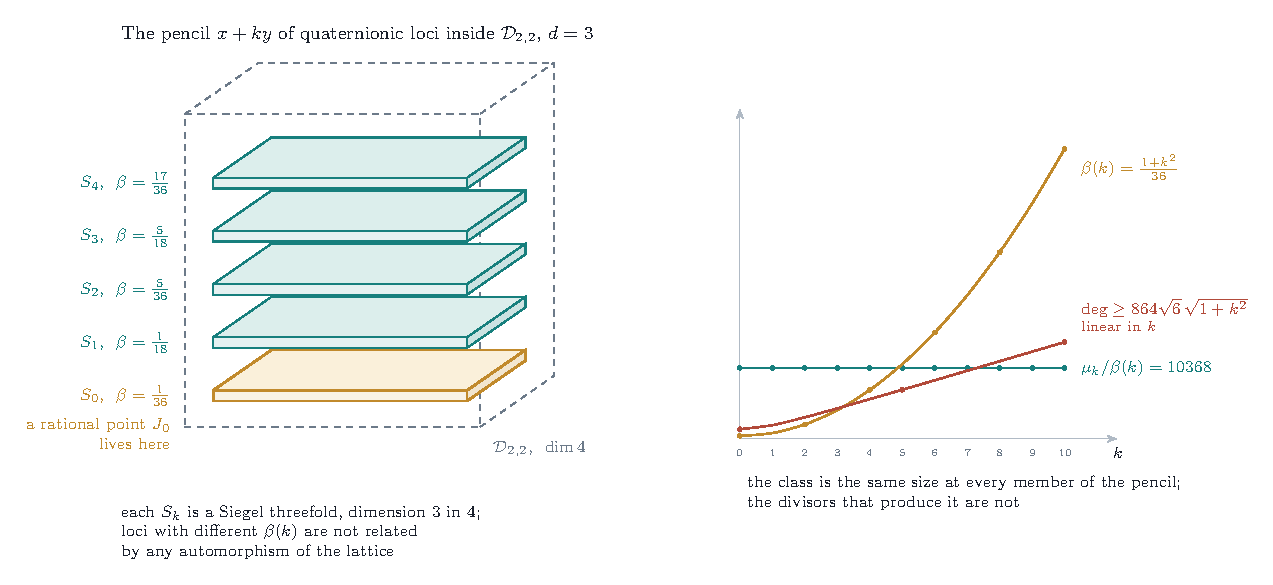
\includegraphics[width=\textwidth]{fig_pencil}
\caption{\Cref{prop:pencil} at $d=3$. Left: the members $S_{k}$ of the
pencil, each a Siegel threefold inside the four-dimensional family, with the
member $k=0$, where $\beta=\tfrac{1}{36}$ is a square and a rational point
$J_{0}$ can be written down, drawn apart. Right: along the pencil the ratio
$\mu_{k}/\beta(k)$ is the constant $10368=\int\eta^{4}/3$, so $\mu_{k}$
grows like $k^{2}$ and the least degree of a divisor not proportional to
$\eta$ grows linearly in $k$. The Weil class is a flat class of the one fixed
lattice and does not change; the divisors that produce it must.}
\label{fig:pencil}
\end{figure}

\begin{remark}[The case $n=2$]\label{rem:ntwo}
Let $n=2$, so $\dim\cS=n^{2}=4$. For every $n$ the quaternionic locus of
\Cref{setup:quat} has dimension $n(n+1)/2$, by a Morita argument. The
quaternion algebra $B=(-d,b)$ contains $K$ and acts on $V$, and
$B\otimes\RR\cong M_{2}(\RR)$ because $b>0$, so Morita equivalence writes
$V_{\RR}$ as $W\otimes_{\RR}\RR^{2}$ with $W$ symplectic of dimension $2n$.
The complex structures commuting with $B$ and compatible with $E$ are then
the complex structures on $W$ compatible with its symplectic form, that is the
points of the Siegel
space $\mathfrak{H}_{n}$, of dimension $n(n+1)/2$, and the codimension in
$\cD_{n,n}$ is $n^{2}-n(n+1)/2=n(n-1)/2$. At
$n=2$ the quaternionic locus is therefore the symmetric space of
$\Sp(4,\RR)$ inside $\cD_{2,2}$, of dimension $3$, so it is a divisor. Its
$G(\QQ)$-translates are infinitely many
pairwise distinct irreducible closed subvarieties of $\cS$ of dimension $3$,
since a finite union of proper closed analytic subsets cannot be dense. If
infinitely many of them carry cycles with one and the same data
$(\underline{P},\underline{q})$, then the closed set
$\Sigma_{\underline{P},\underline{q}}$ has an irreducible component containing
infinitely many distinct irreducible threefolds, so that component has
dimension at least $4$ and therefore equals $\cS$. No density is needed at
$n=2$, only infinitude. Combined with the theorem of Moonen and Zarhin
\cite{MZ99} that every Hodge class on an abelian fourfold lies in the
subalgebra generated by divisor classes and Weil classes, the conclusion would
be the Hodge conjecture for all abelian fourfolds of Weil type, hence for all
abelian fourfolds. That conclusion is a theorem of Markman
\cite[Corollary~1.6.1]{Mar25a}, proved by a different route, so at $n=2$ the
argument above would give a second proof; its interest lies in $n\ge3$.
\end{remark}

\subsection{The second criterion: a rank at one point}

The other way from a dense algebraic locus to an open one is to make the
cycle move, and the classical tool for that is semiregularity. The theorem
below adds nothing to the theory of semiregularity itself. Its content is
that, after \Cref{thm:hdgcount}, \Cref{thm:everyfamily} and
\Cref{thm:closedlocus}, the semiregularity of a single object at a single
point implies the Hodge conjecture for the whole family, with no further
propagation argument. We begin with the object: it exists, and its Chern
character is concentrated in one degree and is a flat Hodge class on the
whole family.

\begin{proposition}[The $K$-theory class at a base point]\label{prop:ktheory}
Let $s_{0}\in\Sigma$ be a base point of \Cref{thm:everyfamily} and write
$A_{0}=A_{s_{0}}$. There are an integer $N\ge1$ and a perfect complex $E$ on
$A_{0}$ with
\[
  \ch_{k}(E)=0\ \ (k\ne n),\qquad \ch_{n}(E)=N\,\omega_{1} .
\]
The tuple $v=\ch(E)$ extends to a flat section of
$\bigoplus_{k}R^{2k}f_{*}\QQ$ over $\cS$ which is of type $(k,k)$ at every
point.
\end{proposition}

\begin{proof}
By \Cref{thm:everyfamily} there is $\xi\in\CH^{n}(A_{0})_{\QQ}$ with
$\cl(\xi)=\omega_{1}$. For a smooth quasi-projective variety over a field the
Chern character $\ch\colon K_{0}(A_{0})_{\QQ}\to\CH^{*}(A_{0})_{\QQ}$ is a
ring isomorphism \cite[Ex.~15.2.16(b) and Cor.~18.3.2]{Ful98}, so there is a
unique $u\in K_{0}(A_{0})_{\QQ}$ with $\ch(u)=\xi$, and its Chern character
has no component outside degree $n$. Choose $N\ge1$ such that $Nu$ is the
image of a class in $K_{0}(A_{0})$; that class is a difference of classes of
vector bundles, hence the class of a perfect complex $E$, and
$\ch(E)=N\xi$. Passing to cohomology gives the displayed identities.

For the last sentence, $\ch(E)$ has a single nonzero component, equal to
$N\omega_{1}$, and $\omega$ is a flat section of type $(n,n)$ everywhere by
\Cref{lem:omegadescends}.
\end{proof}

\begin{theorem}[Buchweitz and Flenner \cite{BF03}; Pridham \cite{Pri24}]\label{thm:BF}
Let $X$ be a smooth projective complex variety, $E$ a perfect complex on $X$,
and $X\hookrightarrow\cX\to\Spec R$ a deformation of $X$ over an Artin local
$\CC$-algebra along which $\ch(E)$ stays of Hodge type. If the semiregularity
map
\[
  \sigma_{E}\colon\Ext^{2}_{X}(E,E)
  \longrightarrow\bigoplus_{q\ge0}H^{q+2}(X,\Omega^{q}_{X}),
  \qquad
  \sigma_{E}(\zeta)=\sum_{q}\tfrac{1}{q!}\,
    \mathrm{tr}\bigl(\zeta\circ\mathrm{At}(E)^{q}\bigr),
\]
is injective, then $E$ extends to a perfect complex on $\cX$.
\end{theorem}

In this generality, for perfect complexes and for every obstruction
annihilated by $\sigma_{E}$ rather than only the curvilinear ones, the
theorem is proved by Pridham \cite{Pri24}, who identifies $\sigma_{E}$ with the
tangent map of a generalised Abel--Jacobi map on the derived moduli of perfect
complexes; for coherent sheaves see also \cite{BLM23}. Perry \cite{Per26}
extends it to noncommutative varieties with group actions, which covers
twisted derived categories and answers a question of Markman.

\begin{theorem}[Semiregularity at one point closes the family]
\label{thm:semiregclosure}
Let $n\ge2$, let $s_{0}$ and $E$ be as in \Cref{prop:ktheory}, and suppose the
semiregularity map $\sigma_{E}$ of \Cref{thm:BF} is injective. Then
$\Sigma=\cD_{n,n}$, and the Hodge conjecture holds in every degree for every
abelian $2n$-fold of $(K,-1,n)$-Weil type with $\Hg(A)=\SU(V,H)$ in that
family.
\end{theorem}

\begin{proof}
Let $\mathfrak{M}$ be the stack of perfect complexes with vanishing negative
self-extensions on the fibres of $f\colon\cA\to\cS$. It is algebraic and
locally of finite presentation over $\cS$ \cite{Lie06}, and at a point $[E]$
over $s_{0}$ its deformation theory relative to $\cS$ has tangent space
$\Ext^{1}(E,E)$ and obstruction space $\Ext^{2}(E,E)$. If
$\Ext^{<0}(E,E)\ne0$, which that stack excludes,\footnote{Lieblich's
stack parametrises the complexes he calls universally gluable, those with
$\Ext^{<0}(E,E)=0$; without that condition a complex can have automorphisms
of negative degree, and the natural moduli object is the derived stack of
To\"en and Vaqui\'e.} use instead the analytic Kuranishi germ of pairs from
the proof of \Cref{thm:p2false}, which has the same tangent and obstruction
spaces; the argument below then gives a nonempty analytic open set in place of
a Zariski open one, which is all that \Cref{cor:allornothing} needs.

By \Cref{prop:ktheory} the Chern character of $E$ stays of Hodge type along
every direction in $\cS$, because it is a flat section of Hodge classes on the
whole base. So \Cref{thm:BF} applies to every infinitesimal deformation of
$A_{0}$ inside the family, and injectivity of $\sigma_{E}$ kills every
obstruction. The morphism $\mathfrak{M}\to\cS$ is therefore formally smooth at
$[E]$, and being locally of finite presentation it is smooth on an open
neighbourhood of $[E]$, which we take connected. Smooth morphisms are open,
so the image of that neighbourhood is a nonempty Zariski open subset
$U\subseteq\cS$.

For $s\in U$ pick a point of the neighbourhood over $s$, that is, a perfect
complex $E_{s}$ on $A_{s}$. Chern characters are locally constant in
families, so $\ch(E_{s})$ is the parallel transport of $\ch(E)$: it is
$N\omega_{1}$ in degree $n$ and zero elsewhere. Chern characters of perfect
complexes are algebraic, so $N\omega_{1}$, and hence $\omega_{1}$, is
algebraic on $A_{s}$; the rest of the Weil line follows by
\Cref{lem:onecomponent}. So $p^{-1}(U)\subseteq\Sigma$, which therefore
contains a nonempty open set, and \Cref{cor:allornothing} gives
$\Sigma=\cD_{n,n}$. Apply \Cref{thm:residual}(a).
\end{proof}

\begin{remark}[The hypothesis is not met by the object above]
\label{rem:semiregunavailable}
Injectivity of $\sigma_{E}$ is automatic for some objects and not for
others, and its degree-zero component already shows both. For a line bundle
$L$ one has $\Ext^{2}(L,L)=H^{2}(\cO_{X})$ and $\sigma_{0}=\mathrm{tr}$ is the
identity on it, so $\sigma_{L}$ is injective for every line bundle on every
variety, and \Cref{thm:BF} returns the classical fact that a divisor class
deforms wherever it stays of type $(1,1)$. The object of \Cref{prop:ktheory}
has rank zero, so its trace component is not an isomorphism, and in general
not injective, the source having no reason to be as small as
$h^{2}(\cO_{A_{0}})=\binom{2n}{2}$. The hypothesis of
\Cref{thm:semiregclosure} therefore rests on the components with $q\ge1$,
which is where semiregularity stops being formal and becomes a computation.

For the object of \Cref{prop:ktheory} the hypothesis fails: by
\Cref{prop:concentrated} it has $\dim\ker\sigma_{E}\ge n^{2}$ at every base
point constructed in this paper (see also \Cref{rem:killsreduction}). The
hypothesis concerns a choice of perfect complex representing a class in
$K_{0}$, and \Cref{prop:concentrated} does not reach every representative.
\Cref{thm:p2forces} and the results after it describe what a representative
satisfying the hypothesis would have to look like, and \Cref{thm:p2false}
shows that there is none. The proof of \Cref{thm:semiregclosure} applies word
for word to the polarised criterion \textup{(P2$'$)} of \Cref{rem:p2prime},
and \Cref{rem:p2primesurvive} records which of the results below carry over
to it.
\end{remark}

\subsection{Consequences of the rank condition}

The hypothesis of \Cref{thm:semiregclosure} is a condition on a rank, which
cannot be inspected until the object is written down. It nevertheless has
consequences that hold for every representative at once, because the
semiregularity map composed with the evaluation map of Hochschild cohomology
is contraction into the Chern character (\Cref{setup:criterion}), and the
Chern character here is a Weil class. The annihilator of a Weil class in
$HT^{2}$ is large, and injectivity forces the evaluation map to vanish on the
whole of it. We compute the annihilator and draw the consequences. They are
the exact analogue for (P2) of what \Cref{thm:candidatefails} and
\Cref{thm:nosplit} do for the secant route in \Cref{sec:secantobjects}, and
they rest on the same local products.

\begin{theorem}[Consequences of injectivity]
\label{thm:p2forces}
Let $A$ be an abelian $2n$-fold of $(K,-1,n)$-Weil type, $n\ge2$, and write
$H^{1}(A,\CC)=V_{+}\oplus V_{-}$ for the eigenspaces of $K$,
$V_{\pm}^{1,0}$, $V_{\pm}^{0,1}$ for their Hodge components and
$T_{\pm}\subset H^{0}(T_{A})=T_{0}A$ for the eigenspaces of $K$ on the tangent
space, each of dimension $n$. Let $\omega=a\alpha_{+}+b\alpha_{-}$ be a
class on the Weil line with $ab\ne0$, for instance any nonzero rational one,
and let $E$ be a nonzero perfect complex on $A$ with $\ch(E)=N\omega$,
$N\ne0$, and no other component.
\begin{enumerate}[label=\textup{(\roman*)},leftmargin=2.6em,itemsep=2pt]
\item The annihilator of $\ch(E)$ in $HT^{2}(A)$ is
  \[
    \Ann_{HT^{2}}(\ch E)
    =\bigl(V_{+}^{0,1}\otimes V_{-}^{0,1}\bigr)
    \;\oplus\;\Hom_{K}\bigl(H^{1,0},H^{0,1}\bigr)
    \;\oplus\;\bigl(T_{+}\otimes T_{-}\bigr),
  \]
  of dimension $n^{2}+2n^{2}+n^{2}=4n^{2}$: the mixed block of $H^{0,2}$,
  which is the annihilator of \Cref{lem:annihilator}; the $K$-linear first
  order deformations of $A$, which contain the tangent space of the polarised
  Weil family; and the mixed bivectors.
\item If $\sigma_{E}$ is injective, then $\operatorname{ev}_{E}$ vanishes on
  this space. Explicitly: $z\cdot\id_{E}=0$ for every $z\in V_{+}^{0,1}\otimes
  V_{-}^{0,1}$; $E$ extends to first order along every $K$-linear deformation
  of $A$; and the translation classes satisfy $A_{\theta}A_{\theta'}=0$ in
  $\Ext^{2}(E,E)$ for every $\theta\in T_{+}$ and $\theta'\in T_{-}$.
\item Under the same hypothesis the algebra map $H^{*}(\cO_{A})\to\Ext^{*}(E,E)$,
  $z\mapsto z\cdot\id_{E}$, kills the ideal generated by the mixed block,
  which is $\bigoplus_{a,b\ge1}\bigwedge^{a}V_{+}^{0,1}\otimes\bigwedge^{b}V_{-}^{0,1}$;
  so the image of $H^{0,k}(A)$ has dimension at most $2\binom{n}{k}$ for
  $1\le k\le n$ and is zero for $k>n$, and every endomorphism $f$ of $E$ has
  $\operatorname{tr}(f)=0$ in $H^{0}(\cO_{A})=\CC$.
\item Under the same hypothesis, if at some point $p$ of its support $E$ is
  locally isomorphic to $i_{*}F$ with $F$ locally free of positive rank on a
  smooth closed subvariety $Z\ni p$ of codimension at least two, then
  $T_{+}\subseteq T_{p}Z$ or $T_{-}\subseteq T_{p}Z$.
\end{enumerate}
\end{theorem}

\begin{proof}
(i) Write $H^{*}(A,\CC)=\bigwedge^{*}(H^{1,0}\oplus H^{0,1})$ and
$\alpha_{\pm}$ for a generator of $\bigwedge^{2n}V_{\pm}
=\bigwedge^{n}V_{\pm}^{1,0}\otimes\bigwedge^{n}V_{\pm}^{0,1}$. The three
summands of $HT^{2}$ act as follows: $z\in H^{0,2}=\bigwedge^{2}H^{0,1}$ by
wedge product; $v\in H^{1}(T_{A})=\Hom(H^{1,0},H^{0,1})$ as the derivation
that replaces one $(1,0)$ factor by its image; $\pi\in H^{0}(\bigwedge^{2}T_{A})
=\bigwedge^{2}(H^{1,0})^{\vee}$ by double contraction of $(1,0)$ factors. For
$z$, the computation is \Cref{lem:annihilator}. For $v$, decompose
$\Hom(H^{1,0},H^{0,1})$ into its four blocks by eigenspaces. An element of
the block $\Hom(V_{+}^{1,0},V_{+}^{0,1})$ replaces a factor of
$\bigwedge^{n}V_{+}^{1,0}$ in $\alpha_{+}$ by an element of $V_{+}^{0,1}$,
which is already exhausted in $\alpha_{+}$, so it kills $\alpha_{+}$; it acts
trivially on $\alpha_{-}$,
which has no $V_{+}^{1,0}$ factor. Likewise $\Hom(V_{-}^{1,0},V_{-}^{0,1})$
kills $\omega$. A nonzero element of the block $\Hom(V_{+}^{1,0},V_{-}^{0,1})$
carries $\alpha_{+}$ to a nonzero element of
$\bigwedge^{n-1}V_{+}^{1,0}\otimes V_{-}^{0,1}\otimes\bigwedge^{n}V_{+}^{0,1}$
and kills $\alpha_{-}$, and a nonzero element of $\Hom(V_{-}^{1,0},V_{+}^{0,1})$
carries $\alpha_{-}$ to a nonzero element of a different summand of
$H^{n-1,n+1}$ and kills $\alpha_{+}$. Since $ab\ne0$ and the two summands are
independent, $v$ kills $\omega$ if and only if its two mixed blocks vanish,
that is, if and only if $v$ is $K$-linear. The space of $K$-linear maps has
dimension $2n^{2}$, and it contains the $n^{2}$-dimensional tangent space of
the polarised family, which is its symmetric part. For $\pi$, a mixed
bivector $\theta\wedge\theta'$ with $\theta\in T_{+}=(V_{+}^{1,0})^{\vee}$ and
$\theta'\in T_{-}=(V_{-}^{1,0})^{\vee}$ kills $\alpha_{+}$ because $\theta'$
kills every factor of $\bigwedge^{n}V_{+}^{1,0}$, and kills $\alpha_{-}$
symmetrically; a nonzero bivector in $\bigwedge^{2}T_{+}$ carries $\alpha_{+}$
to a nonzero element of $\bigwedge^{n-2}V_{+}^{1,0}\otimes\bigwedge^{n}V_{+}^{0,1}$
and kills $\alpha_{-}$, and symmetrically for $\bigwedge^{2}T_{-}$, the two
images lying in different summands; so the annihilator in
$H^{0}(\bigwedge^{2}T_{A})$ is $T_{+}\otimes T_{-}$. Since the images of the
three summands of $HT^{2}$ lie in the three different Hodge components
$H^{n,n+2}$, $H^{n-1,n+1}$ and $H^{n-2,n}$ of $H^{*}(A,\CC)$, the annihilator
is the direct sum of the three annihilators computed, of dimensions $n^{2}$,
$2n^{2}$ and $n^{2}$.

(ii) By the commutative square $\sigma_{E}\circ\operatorname{ev}_{E}
=(\,\cdot\,)\lrcorner\ch(E)$ of \Cref{setup:criterion}, $\sigma_{E}$
vanishes on $\operatorname{ev}_{E}(\Ann_{HT^{2}}(\ch E))$; if $\sigma_{E}$
is injective, $\operatorname{ev}_{E}$ vanishes there. The three explicit
statements are \eqref{eq:evgeneral} on the three summands of (i): on
$H^{0,2}$ the evaluation map is $z\mapsto z\cdot\id_{E}$; on $H^{1}(T_{A})$
it is the obstruction map $v\mapsto v\lrcorner\mathrm{At}(E)$, whose
vanishing on $v$ is the extension of $E$ to first order along $v$
\cite{Tod09}; and on a bivector $\theta\wedge\theta'$ it is
$\tfrac12(\theta\wedge\theta')\lrcorner\mathrm{At}(E)^{2}
=A_{\theta}A_{\theta'}$, as in the proof of \Cref{thm:candidatefails}.

(iii) The map $z\mapsto z\cdot\id_{E}$ is a homomorphism of graded algebras
from $H^{*}(\cO_{A})=\bigwedge^{*}H^{0,1}$ to the graded centre of the Yoneda
algebra, so its kernel is an ideal, and by (ii) it contains the mixed block
$V_{+}^{0,1}\otimes V_{-}^{0,1}$. The ideal generated by the mixed block in
$\bigwedge^{*}(V_{+}^{0,1}\oplus V_{-}^{0,1})
=\bigwedge^{*}V_{+}^{0,1}\otimes\bigwedge^{*}V_{-}^{0,1}$ is the sum of the
summands $\bigwedge^{a}V_{+}^{0,1}\otimes\bigwedge^{b}V_{-}^{0,1}$ with
$a,b\ge1$, since each such summand consists of multiples of the mixed block,
while the remaining summands, with $a=0$ or $b=0$, meet the ideal in zero; the
quotient in degree $k\ge1$ is $\bigwedge^{k}V_{+}^{0,1}\oplus\bigwedge^{k}V_{-}^{0,1}$,
of dimension $2\binom{n}{k}$, and zero for $k>n$. In particular the top class
of $H^{2n}(\cO_{A})$, which is mixed for $n\ge1$, acts by zero. Serre duality
on $A$, whose canonical bundle is trivial, is the perfect pairing
$\Ext^{2n}(E,E)\times\Hom(E,E)\to H^{2n}(\cO_{A})\cong\CC$,
$(\xi,f)\mapsto\operatorname{tr}(\xi\circ f)$; for $\xi=w\cdot\id_{E}$
with $w$ the top class this is $w\cdot\operatorname{tr}(f)$, where
$\operatorname{tr}(f)\in H^{0}(\cO_{A})=\CC$, so $w\cdot\id_{E}=0$ forces
$\operatorname{tr}(f)=0$ for every $f$.

(iv) Let $\cO$ be the local ring of $A$ at $p$ and choose coordinates with
$Z=\{x_{1}=\dots=x_{c}=0\}$, $c\ge2$. Locally $E\cong(\cO/J)^{\oplus r}$
with $J=(x_{1},\dots,x_{c})$, a regular sequence, so
$\Ext^{*}_{\cO}(\cO/J,\cO/J)=\bigwedge^{*}_{\cO/J}N$ as a graded algebra,
where $N=\Hom(J/J^{2},\cO/J)$ is the normal module with basis the classes
$\partial_{1},\dots,\partial_{c}$ dual to $x_{1},\dots,x_{c}$; the
$\Ext^{1}$ is computed on the Koszul resolution exactly as in the proof of
\Cref{lem:localproducts}, and the product is the wedge because the Yoneda
algebra of a Koszul complex is the exterior algebra on the dual of the
generators. For $E$ of rank $r$ the local Yoneda algebra is
$\bigwedge^{*}N\otimes M_{r}(\cO/J)$. By \Cref{lem:edge} the germ of
$A_{\theta}$ at $p$ is the jet class along $\theta$; on the Koszul complex the
jet class of a derivation $D$ is the chain map $-D(d)$, and for
$D=\theta=\sum_{i}c^{i}\partial_{i}$ its component in $\Ext^{1}=N\otimes M_{r}(\cO/J)$
is $\sum_{i\le c}(c^{i}\bmod J)\,\partial_{i}\otimes\id$, the class of
$\theta$ modulo $T_{Z}$. Multiplicativity of the germ map then gives the germ
of $A_{\theta}A_{\theta'}$ as
$(\theta\bmod T_{Z})\wedge(\theta'\bmod T_{Z})\otimes\id$ in
$\bigwedge^{2}N\otimes M_{r}(\cO/J)$, whose value at $p$ is
$\bar\theta(p)\wedge\bar\theta'(p)\in\bigwedge^{2}(T_{p}A/T_{p}Z)$. If
$A_{\theta}A_{\theta'}=0$ for all $\theta\in T_{+}$, $\theta'\in T_{-}$,
then $\bar a\wedge\bar b=0$ for all $\bar a$ in the image $I_{+}$ of $T_{+}$
and $\bar b$ in the image $I_{-}$ of $T_{-}$ in $N_{p}=T_{p}A/T_{p}Z$, and
$I_{+}+I_{-}=N_{p}$ since $T_{+}\oplus T_{-}=T_{p}A$. If both $I_{\pm}$ were
nonzero, every nonzero $\bar b\in I_{-}$ would be proportional to every
nonzero $\bar a\in I_{+}$, so $I_{+}=I_{-}$ would be a line and
$N_{p}=I_{+}+I_{-}$ of dimension one, against $c\ge2$. Hence $I_{+}=0$ or
$I_{-}=0$, which is the claim.
\end{proof}

\begin{corollary}[Locally free components are excluded]\label{cor:p2shape}
Let $A$ be as in \Cref{thm:p2forces} and suppose that no proper abelian
subvariety $B\subset A$ has $T_{0}B\supseteq T_{+}$ or $T_{0}B\supseteq T_{-}$;
equivalently, that $A$ has no nonzero $K$-stable abelian subvariety on which
$K$ acts through a single embedding. This holds whenever $A$ is simple, at
every split member $X\times\widehat X$ with $X$ simple of endomorphism
algebra $\QQ$, and at a general point of the quaternionic locus of
\Cref{setup:quat}.
Let $E$ be a perfect complex on $A$ with $\ch(E)=N\omega$ as above and
$\sigma_{E}$ injective. Then no irreducible component $Z_{0}$ of the support
of $E$ of codimension at least two has a dense open subset along which $E$ is
a locally free sheaf of positive rank on $Z_{0}$. In particular $E$ is not a
sheaf, and along every component of its support of codimension at least two
it has, generically, either at least two nonvanishing cohomology sheaves or a
cohomology sheaf that is not locally free on the reduced support.
\end{corollary}

\begin{proof}
Suppose that $Z_{0}$ is such a component, with $U\subseteq Z_{0}^{\mathrm{sm}}$
dense open and $E|_{U}$ a locally free sheaf of positive rank on $U$. By
\Cref{thm:p2forces}(iv), $U=U_{+}\cup U_{-}$ with
$U_{\pm}=\{p\in U:T_{\pm}\subseteq T_{p}Z_{0}\}$, both closed in $U$; as $U$
is irreducible, $U=U_{+}$ say. Then every constant vector field
$\theta\in T_{+}$ is tangent to $Z_{0}$ along $U$, hence along
$Z_{0}^{\mathrm{sm}}$. The set
$S=\{(p,t)\in Z_{0}\times\CC:p+\exp(t\theta)\in Z_{0}\}$ is a closed
analytic subset of the irreducible space $Z_{0}\times\CC$, and it contains
an open neighbourhood of $Z_{0}^{\mathrm{sm}}\times\{0\}$, because the local
flow of the restriction of $\theta$ to the submanifold $Z_{0}^{\mathrm{sm}}$
exists on such a neighbourhood; so $S=Z_{0}\times\CC$, and
$Z_{0}+\exp(t\theta)\subseteq Z_{0}$, hence $=Z_{0}$, for every $t$. Let
$G=\{x\in A:Z_{0}+x=Z_{0}\}$, a closed algebraic subgroup of $A$, and $B$
its identity component, an abelian subvariety. The connected set
$\exp(T_{+})$ contains $0$ and lies in $G$, hence in $B$, so
$T_{+}\subseteq T_{0}B$. By hypothesis $B=A$, so $Z_{0}=A$, against the
codimension. The last sentence of the statement is the negation of the
condition just excluded. If $E$ were a sheaf, its support would have
codimension at least $n$, because the Chern character of a nonzero sheaf
begins in the codimension of its support, with the support cycle, whose
multiplicities are positive; this is excluded by \Cref{thm:p2support}(iii)
below, whose proof uses nothing from the present one beyond the translation
argument above.

For the equivalence in the hypothesis, let $\sqrt{-d}$ act on $A$ through
an order of $K$. If an abelian subvariety $B\ne A$ has
$T_{0}B\supseteq T_{+}$, then $H_{1}(B,\QQ)\cap\sqrt{-d}\,H_{1}(B,\QQ)$ is a
$K$-stable sub-Hodge structure, hence $H_{1}(C,\QQ)$ for a $K$-stable abelian
subvariety $C\subseteq B$, and $T_{0}C=T_{0}B\cap\sqrt{-d}\,T_{0}B$ still
contains $T_{+}$, on which $\sqrt{-d}$ acts by a scalar. The $K$-stable
complement $C'$ of $C$ for the polarisation is nonzero, since
$C\subseteq B\ne A$, and $T_{0}C'$ is a $K$-stable complement of
$T_{0}C\supseteq T_{+}$, so $T_{0}C'\subseteq T_{-}$ and $K$ acts on $C'$
through a single embedding. Conversely, if a nonzero $K$-stable $C'\ne A$ has
$T_{0}C'\subseteq T_{-}$, its $K$-stable complement $B$ is proper with
$T_{0}B\supseteq T_{+}$. For the three cases: a simple $A$ has no nonzero
proper abelian subvariety; for $X\times\widehat X$ with $X$ simple and
$\End^{0}(X)=\QQ$ the sub-Hodge structures of $H_{1}(X)\otimes\QQ^{2}$ are
$H_{1}(X)\otimes W$ with $W\subseteq\QQ^{2}$, and since $K$ acts on
$\QQ^{2}$ through a quadratic field, $W$ is $K$-stable only for $W=0$ or
$\QQ^{2}$; and at a general quaternionic member $A$ is either simple or, when
the quaternion algebra of \Cref{setup:quat} splits, isogenous to $C\times C$
with $C$ a general
principally polarised abelian $n$-fold, whose sub-Hodge structures are again
$H_{1}(C)\otimes W$ with the same conclusion.
\end{proof}

\subsection{The Hochschild action and the two branches}

\Cref{thm:p2forces} computes the annihilator summand by summand and reads off
what the vanishing of the evaluation map on it means for $E$. That
description hides a structure which is easily brought out and gives more:
the annihilator is the mixed part of a splitting of $HH^{1}(A)$ into two
halves, one for each of the two conjugate pieces $\alpha_{+}$ and
$\alpha_{-}$ of the Weil class, and the same splitting describes the
annihilator in every degree. The results of this subsection concern the
Hochschild cohomology of $A$ alone, and their consequences for $E$ follow
formally.

\begin{setupenv}[Hochschild cohomology in these terms]\label{setup:hh}
For an abelian variety $A$ the Hochschild--Kostant--Rosenberg isomorphism
identifies
\[
  HH^{*}(A)\;\cong\;HT^{*}(A)=\bigoplus_{p,q}H^{p}\bigl(\textstyle\bigwedge^{q}T_{A}\bigr)
  =\textstyle\bigwedge^{*}\bigl(H^{0,1}(A)\oplus H^{0}(T_{A})\bigr),
\]
as graded rings, the grading being $p+q$: the Todd class of $A$ is trivial,
so the twist by $\td^{1/2}$ in \cite{Cal05}, \cite{CRV12} is the identity and
the plain identification is already multiplicative. Write
$HH^{1}(A)=H^{0,1}(A)\oplus H^{0}(T_{A})$, of dimension $4n$, so that
$HH^{*}(A)$ is the exterior algebra on it, of dimension $2^{4n}$. It acts on
$H^{*}(A,\CC)=\bigwedge^{*}\bigl(H^{1,0}\oplus H^{0,1}\bigr)$ by wedging with
the classes of $H^{0,1}$ and contracting the classes of $H^{1,0}$ against
$H^{0}(T_{A})$; the two families of operators involve disjoint generators, so
they pairwise anticommute and the action is an action of the exterior algebra.
In degree two this is the operator $x\lrcorner$ of \Cref{setup:criterion}, and
$\operatorname{ev}_{E}\colon HH^{*}(A)\to\Ext^{*}(E,E)$ is a homomorphism of
graded rings into the graded centre, with
$\sigma_{E}\circ\operatorname{ev}_{E}=(\,\cdot\,)\lrcorner\ch(E)$
\cite[Section 6]{BF08}, \cite{Cal05}, \cite{CRV12}.
\end{setupenv}

\begin{theorem}[The annihilator is the mixed part of a splitting]
\label{thm:hhsplitting}
Let $A$ be of $(K,-1,n)$-Weil type with $n\ge2$, and let
$\omega=a\alpha_{+}+b\alpha_{-}$ lie on the Weil line with $ab\ne0$. Put
\[
  P=\Ann_{HH^{1}}(\alpha_{+})=V_{+}^{0,1}\oplus T_{-},
  \qquad
  Q=\Ann_{HH^{1}}(\alpha_{-})=V_{-}^{0,1}\oplus T_{+} .
\]
\begin{enumerate}[label=\textup{(\roman*)},leftmargin=2.6em,itemsep=2pt]
\item $\dim P=\dim Q=2n$ and $HH^{1}(A)=P\oplus Q$; in particular
  $\Ann_{HH^{1}}(\omega)=0$.
\item $\Ann_{HH^{2}}(\omega)=P\wedge Q$, of dimension $4n^{2}$. This is the
  space computed in \Cref{thm:p2forces}(i), written as the mixed part of the
  splitting.
\item Contraction with $\alpha_{-}$ is injective on $\bigwedge^{*}P$, and
  contraction with $\alpha_{+}$ is injective on $\bigwedge^{*}Q$; the two
  images meet in exactly one line, in degree $2n$.
\item For every $k\ge1$,
  \[
    \Ann_{HH^{k}}(\omega)
    =\Bigl(\bigoplus_{\substack{i+j=k\\ i,j\ge1}}
      \textstyle\bigwedge^{i}P\wedge\bigwedge^{j}Q\Bigr)\;\oplus\;\epsilon_{k},
  \]
  where $\epsilon_{k}=0$ for $k\ne2n$ and $\epsilon_{2n}$ is the line of
  \textup{(iii)}. So
  $\dim\Ann_{HH^{k}}(\omega)=\binom{4n}{k}-2\binom{2n}{k}+\delta_{k,2n}$ for
  $k\ge1$, while $\Ann_{HH^{0}}(\omega)=0$, and the annihilator is the ideal
  generated by its degree-two part together with that one line.
\end{enumerate}
\end{theorem}

\begin{proof}
Choose bases $x_{1},\dots,x_{n}$ of $V_{+}^{1,0}$ and $y_{1},\dots,y_{n}$ of
$V_{-}^{1,0}$, and bases $\bbar x_{i}$ of $V_{+}^{0,1}$ and $\bbar y_{j}$ of
$V_{-}^{0,1}$ (the bar is notation only: complex conjugation carries
$V_{+}^{1,0}$ to $V_{-}^{0,1}$), so that
$\alpha_{+}=x_{1}\cdots x_{n}\bbar x_{1}\cdots\bbar x_{n}$ and
$\alpha_{-}=y_{1}\cdots y_{n}\bbar y_{1}\cdots\bbar y_{n}$, and write
$\partial_{x_{i}},\partial_{y_{j}}$ for the dual basis of
$H^{0}(T_{A})=T_{+}\oplus T_{-}$.

(i) Of the $4n$ basis operators, $\bbar x_{i}\wedge$ kills $\alpha_{+}$
because $\bbar x_{i}$ already occurs in it, and $\partial_{y_{j}}\lrcorner$
kills $\alpha_{+}$ because no $y$ occurs in it; so $P\supseteq
V_{+}^{0,1}\oplus T_{-}$. Conversely, the classes
$\bbar y_{j}\wedge\alpha_{+}$ are linearly independent, as are the classes
$\partial_{x_{i}}\lrcorner\alpha_{+}$, and the two families lie in different
summands of $H^{*}$, so no nonzero combination of the operators
$\bbar y_{j}\wedge$ and $\partial_{x_{i}}\lrcorner$ kills $\alpha_{+}$:
$P=V_{+}^{0,1}\oplus T_{-}$, of dimension $2n$. The computation for $Q$ is the
same with the roles of the two eigenspaces exchanged, and
$P\cap Q=0$ with $\dim P+\dim Q=4n$, so $HH^{1}=P\oplus Q$. A class of degree
one that kills $\omega$ kills $\alpha_{+}$ and $\alpha_{-}$ separately, the
two images lying in different summands and $ab\ne0$, so it lies in
$P\cap Q=0$.

(iii) A monomial $\bbar x_{I}\partial_{y_{J}}\in\bigwedge^{*}P$ sends
$\alpha_{-}$ to $\pm\,\bbar x_{I}\,y_{[n]\setminus J}\,\bbar y_{[n]}$, and
these are linearly independent for distinct pairs $(I,J)$, which is the
injectivity; the statement for $Q$ is symmetric. For the intersection, the
image of $\bigwedge^{*}P$ is spanned by monomials with no factor $x$ and all
$n$ factors $\bbar y$, and the image of $\bigwedge^{*}Q$, by the same
computation, by monomials with no factor $y$ and all $n$ factors $\bbar x$.
Both images are spanned by monomials, so their intersection is spanned by the
monomials common to both, and the only such monomial is
$\bbar x_{[n]}\bbar y_{[n]}$. It is the image of
$\pi_{P}=\bbar x_{[n]}\partial_{y_{[n]}}$ and of
$\pi_{Q}=\bbar y_{[n]}\partial_{x_{[n]}}$, both of degree $2n$. So the
intersection is the single line spanned by that class.

(ii) and (iv) Decompose $\bigwedge^{k}HH^{1}=\bigoplus_{i+j=k}\bigwedge^{i}P
\wedge\bigwedge^{j}Q$. A summand with $i,j\ge1$ annihilates $\alpha_{+}$,
because it has a factor in $P$ and the action is an action of the algebra, and
annihilates $\alpha_{-}$ for the same reason with $Q$; so it lies in the
annihilator of $\omega$. The sum of these summands over all $k$ is the ideal
generated by $P\wedge Q$, since each of their monomials has, after
reordering, a factor $p\wedge q$ with $p\in P$ and $q\in Q$. On the remaining
two summands, $\xi_{P}\in\bigwedge^{k}P$ has
$\xi_{P}\lrcorner\omega=b\,\xi_{P}\lrcorner\alpha_{-}$ and
$\xi_{Q}\in\bigwedge^{k}Q$ has $\xi_{Q}\lrcorner\omega=a\,\xi_{Q}\lrcorner\alpha_{+}$,
so a combination $\xi_{P}+\xi_{Q}$ annihilates $\omega$ if and only if
$b\,\xi_{P}\lrcorner\alpha_{-}=-a\,\xi_{Q}\lrcorner\alpha_{+}$. By (iii) both
contractions are injective and their images meet only in degree $2n$, in one
line; so this happens only for $k=2n$, and then only on the line spanned by
$b^{-1}\pi_{P}-a^{-1}\pi_{Q}$, with $\pi_{P}$ and $\pi_{Q}$ scaled so that
$\pi_{P}\lrcorner\alpha_{-}=\pi_{Q}\lrcorner\alpha_{+}$. In degree zero the
annihilator is zero because $\omega\ne0$. Taking $k=2$ and $n\ge2$, so that
$2\ne2n$, gives (ii), the dimension being
$\dim P\cdot\dim Q=4n^{2}$; the general count is
$\binom{4n}{k}-\binom{2n}{k}-\binom{2n}{k}$ plus the exceptional line.
\end{proof}

\begin{corollary}[Consequences for the Hochschild action]
\label{cor:hhfactor}
Let $A$ and $\omega$ be as above and let $E$ be a nonzero perfect complex on
$A$ with $\ch(E)=N\omega$, $N\ne0$.
\begin{enumerate}[label=\textup{(\roman*)},leftmargin=2.6em,itemsep=2pt]
\item Unconditionally, $\dim\Ext^{2}(E,E)\ge2n(2n-1)$.
\item If $\sigma_{E}$ is injective then $\operatorname{ev}_{E}$ vanishes on
  $P\wedge Q$, hence on the ideal it generates, and the ring homomorphism
  $\operatorname{ev}_{E}\colon HH^{*}(A)\to\Ext^{*}(E,E)$ factors through
  \[
    R\;=\;\textstyle\bigwedge^{*}P\;\oplus_{\CC}\;\bigwedge^{*}Q,
    \qquad \dim_{\CC}R=2^{2n+1}-1,
  \]
  the two exterior algebras glued along their scalars, inside $HH^{*}(A)$ of
  dimension $2^{4n}$. At $n=2$ that is $31$ out of $256$.
\item Granting the compatibility
  $\sigma_{E}\circ\operatorname{ev}_{E}=(\,\cdot\,)\lrcorner\ch(E)$ in degree
  $k$ \cite{Cal05}, \cite{CRV12}, the induced map on $R$ is injective away
  from the line of \Cref{thm:hhsplitting}(iii), so
  \[
    \dim\Ext^{k}(E,E)\;\ge\;2\binom{2n}{k}\quad(1\le k<2n),
    \qquad
    \sum_{k\ge1}\dim\Ext^{k}(E,E)\;\ge\;2^{2n+1}-3 .
  \]
\end{enumerate}
\end{corollary}

\begin{proof}
(i) By \Cref{setup:hh}, $\ker\operatorname{ev}_{E}\subseteq\Ann_{HH^{2}}(\ch E)$
in degree two, since $\sigma_{E}(\operatorname{ev}_{E}(\xi))=\xi\lrcorner\ch(E)$
and the right side is nonzero off the annihilator. Hence
$\dim\Ext^{2}(E,E)\ge\dim HH^{2}(A)-\dim\Ann_{HH^{2}}(\omega)
=\binom{4n}{2}-4n^{2}=2n(2n-1)$ by \Cref{thm:hhsplitting}(ii). No hypothesis
on $\sigma_{E}$ is used.

(ii) $\operatorname{ev}_{E}$ vanishes on the annihilator by
\Cref{thm:p2forces}(ii), its kernel is an ideal because it is a ring map, and
the ideal generated by $P\wedge Q$ in $\bigwedge^{*}(P\oplus Q)
=\bigwedge^{*}P\otimes\bigwedge^{*}Q$ is the sum of the summands with
$i,j\ge1$, whose complement is $\bigwedge^{*}P\oplus_{\CC}\bigwedge^{*}Q$ of
dimension $2\cdot2^{2n}-1$.

(iii) With the compatibility in degree $k$, the argument of (i) gives
$\ker\operatorname{ev}_{E}\subseteq\Ann_{HH^{k}}(\omega)$, and by
\Cref{thm:hhsplitting}(iv) that annihilator meets $\bigwedge^{k}P\oplus
\bigwedge^{k}Q$ only in the exceptional line. So the map induced on $R$ has
kernel contained in that one line and its image has dimension at least
$\dim R-1=2^{2n+1}-2$. One of those dimensions sits in degree zero, where the
image is $\CC\cdot\id_{E}$, nonzero because $E$ is; the remaining
$2^{2n+1}-3$ lie in positive degrees, which is the second inequality. For
$1\le k<2n$ the exceptional line has no component in degree $k$, so
$\bigwedge^{k}P\oplus\bigwedge^{k}Q$, of dimension $2\binom{2n}{k}$, maps
injectively, which is the first.
\end{proof}

\begin{remark}[The two branches]\label{rem:twobranches}
The ring $R$ of \Cref{cor:hhfactor}(ii) is the ring of functions on two odd
affine spaces of dimension $2n$ crossing at the origin. In these terms, if $E$
satisfies the criterion, the deformations of $D^{b}(A)$ along which its
Hochschild action survives form two branches, $P$ and $Q$, which meet only at
the trivial deformation and are the annihilators of the two conjugate pieces
$\alpha_{+}$ and $\alpha_{-}$ of the Weil class. The criterion says that $E$
sees the two halves of the class separately and their interaction not at all.

The splitting $HH^{1}=P\oplus Q$ is not the splitting into eigenspaces of
$K$, which are $V_{+}^{0,1}\oplus T_{+}$ and $V_{-}^{0,1}\oplus T_{-}$; $P$
and $Q$ cut across them. It is the splitting into the annihilators of
$\alpha_{+}$ and of $\alpha_{-}$, and it exists because each of the two
pieces of the Weil class is a top form on an eigenspace. Nor is the
conclusion a contradiction in itself. $R$ is a perfectly good ring, and the
bound of (iii) is consistent with the value of $\chi(E,E)$ computed in
\Cref{prop:objectsize}, since $\sum_{k}(-1)^{k}2\binom{2n}{k}=0$. The
corollary says how large such an $E$ must be and how little of the Hochschild
cohomology it may see, but nothing in the Hochschild computation forbids an
$E$ of the required shape. The exclusion comes from a different direction,
deformation to non-algebraic Weil tori, in \Cref{thm:p2false}.
\end{remark}

\subsection{The numerical form of the criterion and the support}

The same square gives two further results. The first converts the rank of
$\sigma_{E}$ into a single dimension, the form in which a candidate can be
tested. The second locates the support of $E$, and it excludes the first
place one would look: a cycle representing the Weil class.

\begin{theorem}[The criterion as a dimension]\label{thm:p2numerical}
Let $A$, $\omega$ and $E$ be as in \Cref{cor:hhfactor}, so that
$\ch(E)=N\omega$ with $N\ne0$ and no other component.
\begin{enumerate}[label=\textup{(\roman*)},leftmargin=2.6em,itemsep=2pt]
\item If $\dim\Ext^{2}(E,E)=2n(2n-1)$, the least value that
  \Cref{cor:hhfactor}(i) allows, then $\operatorname{ev}_{E}\colon
  HH^{2}(A)\to\Ext^{2}(E,E)$ is surjective with kernel exactly $P\wedge Q$,
  the map $\sigma_{E}$ is injective, and every class of $\Ext^{2}(E,E)$ is a
  sum of products $\operatorname{ev}_{E}(p)\operatorname{ev}_{E}(p')
  +\operatorname{ev}_{E}(q)\operatorname{ev}_{E}(q')$ with $p,p'\in P$ and
  $q,q'\in Q$, hence lies in the graded centre of $\Ext^{*}(E,E)$.
\item Conversely, if $\sigma_{E}$ is injective, then
  $\operatorname{ev}_{E}(HH^{2}(A))$ has dimension exactly $2n(2n-1)$, and
  $\sigma_{E}$ carries it isomorphically onto $HH^{2}(A)\lrcorner\,\omega$.
\item Consequently, if at one base point $s_{0}$ of a family some perfect
  complex $E$ with $\ch(E)=N\omega_{1}$ has $\dim\Ext^{2}(E,E)=2n(2n-1)$,
  then $\Sigma=\cD_{n,n}$, and the Hodge conjecture holds in every degree for
  every member of that family with $\Hg(A)=\SU(V,H)$.
\end{enumerate}
\end{theorem}

\begin{proof}
(i) The square of \Cref{setup:hh} gives $\ker\operatorname{ev}_{E}
\subseteq\Ann_{HH^{2}}(\omega)=P\wedge Q$ in degree two, the equality being
\Cref{thm:hhsplitting}(ii). Hence $\operatorname{rank}\operatorname{ev}_{E}
\ge\binom{4n}{2}-4n^{2}=2n(2n-1)=\dim\Ext^{2}(E,E)$, so
$\operatorname{ev}_{E}$ is onto and its kernel, of dimension $4n^{2}$ and
contained in $P\wedge Q$, is all of $P\wedge Q$. Every class of
$\Ext^{2}(E,E)$ is then $\operatorname{ev}_{E}(\xi)$ for some $\xi$, and
$\sigma_{E}(\operatorname{ev}_{E}(\xi))=N\,\xi\lrcorner\,\omega$ vanishes only
for $\xi\in P\wedge Q=\ker\operatorname{ev}_{E}$; so $\sigma_{E}$ is injective.
Since $HH^{2}(A)=\bigwedge^{2}P\oplus(P\wedge Q)\oplus\bigwedge^{2}Q$ and
$\operatorname{ev}_{E}$ is a ring map into the graded centre, the image is
$\operatorname{ev}_{E}(\bigwedge^{2}P)+\operatorname{ev}_{E}(\bigwedge^{2}Q)$,
which is the description of the classes.

(ii) By \Cref{thm:p2forces}(ii) the kernel of $\operatorname{ev}_{E}$ in
degree two contains $P\wedge Q$, and by the argument of (i) it is contained in
it, so it equals $P\wedge Q$ and the image has dimension $2n(2n-1)$. The
composite $\sigma_{E}\circ\operatorname{ev}_{E}$ is contraction into
$\ch(E)=N\omega$, whose kernel is exactly $P\wedge Q=\ker\operatorname{ev}_{E}$,
so $\sigma_{E}$ maps the image isomorphically onto
$HH^{2}(A)\lrcorner\,\omega$.

(iii) By (i) the map $\sigma_{E}$ is injective, and \Cref{thm:semiregclosure}
applies.
\end{proof}

\Cref{thm:p2numerical}(iii) is a sufficient condition for
$\mathbf{W}(K,n,\delta)$ that mentions no map at all: one object, at one
point, and one number. At $n=2$ the number is $12$ and at $n=3$ it is $30$.
By \Cref{thm:p2false} no complex attains it, but the first two parts of the
theorem hold for the polarised criterion (P2$'$) with the number $r(\gamma)$
of \Cref{thm:p2primenumber}(iv) in place of $2n(2n-1)$, and that is the form
in which the polarised criterion can be tested.

The dimension of $\Ext^{2}(E,E)$ is computable in a way the rank of
$\sigma_{E}$ is not. For a complex built from sheaves whose cohomology is
known, the local-to-global spectral sequence
$E_{2}^{p,q}=H^{p}(A,\cE xt^{q}(E,E))\Rightarrow\Ext^{p+q}(E,E)$ reduces the
count to the cohomology of the local $\cE xt$ sheaves, and on an abelian
variety the cohomology of a sheaf supported on an abelian subvariety, or of a
homogeneous bundle, is a question of linear algebra. The rank of
$\sigma_{E}$, by contrast, requires the trace of the exponential of the
Atiyah class on every class of $\Ext^{2}$, a computation with the object and
not only with its invariants. Part (ii) says that, on the central part of
$\Ext^{2}$, nothing is lost by reading the criterion this way. Whether an
injective $\sigma_{E}$ forces the whole of $\Ext^{2}(E,E)$ to be central is,
by Serre duality, a statement about $\Ext^{2n-2}$, which the square in degree
two does not reach; nothing below uses it.

The second result rests on a local fact about complexes supported at a point,
which we state and prove first.

\begin{lemma}[Two jet classes on a complex of finite length]
\label{lem:finiteproduct}
Let $R=\CC[[x_{1},\dots,x_{c}]]$ with $c\ge2$, let $M$ be a bounded complex of
finitely generated free $R$-modules whose cohomology has finite length, and
put $\chi(M)=\sum_{i}(-1)^{i}\ell(H^{i}(M))$. For $a\in\CC^{c}$ let
$J(a)\in\Ext^{1}_{R}(M,M)$ be the jet class of $M$ along the constant vector
field $\sum_{i}a_{i}\partial_{i}$, represented by the chain map
$-\sum_{i}a_{i}\partial_{i}(d)$ as in the proof of \Cref{thm:p2forces}(iv).
If $\chi(M)\ne0$ and $a,b$ are linearly independent, then $J(a)J(b)\ne0$ in
$\Ext^{2}_{R}(M,M)$.
\end{lemma}

\begin{proof}
Let $T$ be an abelian variety of dimension $c$ and $t\in T$ a point. Linear
coordinates on the universal cover identify the completed local ring
$\widehat{\cO}_{T,t}$ with $R$ in such a way that the translation invariant
vector fields become the constant fields $\sum_{i}a_{i}\partial_{i}$: the
exponential map from $T_{t}T=\CC^{c}$ is a local biholomorphism carrying the
constant vector fields to the translation invariant ones, and its germ at the
origin identifies $\widehat{\cO}_{T,t}$ with $\CC[[x_{1},\dots,x_{c}]]$
compatibly with derivations. A complex of $R$-modules with finite length
cohomology is the same thing as a complex of $\cO_{T,t}$-modules with finite
length cohomology, since modules of finite length over either ring are
modules over $\cO_{T,t}/\mathfrak{m}^{N}$ for $N$ large, so $M$ defines a
perfect complex $M_{T}$ on $T$ supported at $t$. Its local $\cE xt$ sheaves
are skyscrapers at $t$, so the local-to-global spectral sequence gives
$\Ext^{*}_{T}(M_{T},M_{T})=\Ext^{*}_{R}(M,M)$, and by \Cref{lem:edge} the
translation classes $A_{a}$, $A_{b}$ of $M_{T}$ restrict to $J(a)$, $J(b)$.
Apply the square of \Cref{setup:criterion} on $T$ to the bivector $a\wedge b$:
\[
  \sigma_{M_{T}}\bigl(A_{a}A_{b}\bigr)=(a\wedge b)\lrcorner\,\ch(M_{T}).
\]
A sheaf of length $\ell$ supported at a point has Chern character
$\ell\cdot[\mathrm{pt}]$, and Chern characters are additive over the
cohomology of a complex, so $\ch(M_{T})=\chi(M)\,[\mathrm{pt}]$. The class of a
point is a nonzero multiple of $dz_{1}\cdots dz_{c}\,d\bbar z_{1}\cdots
d\bbar z_{c}$, and contracting it with $a\wedge b$ removes two holomorphic
factors and leaves a nonzero class of type $(c-2,c)$, because $a$ and $b$ are
independent. So the right side is nonzero when $\chi(M)\ne0$, hence so is
$A_{a}A_{b}$, and so is its restriction $J(a)J(b)$, the restriction map being
an isomorphism.
\end{proof}

The hypothesis on $\chi(M)$ cannot be dropped. The Euler characteristic is
the only additive invariant here: the Grothendieck group of complexes with
finite length cohomology over a regular local ring is $\ZZ$, generated by the
residue field, since every module of finite length has a composition series
whose factors are all isomorphic to it. The lemma says that the product of two
independent jet classes detects this generator, and on a complex of Euler
characteristic zero the product can vanish. Let $K$ be the Koszul resolution
of the residue field $k$ of $\QQ[x_{1},x_{2}]$, on which the jet class of a
derivation $D$ is the chain map $-D(d_{K})$, and let $u=\partial_{2}(d_{K})
\partial_{1}(d_{K})\colon K\to K[2]$ represent $J(\partial_{2})J(\partial_{1})$.
The entries of $d_{K}$ are $\pm x_{1},\pm x_{2}$, so $u$ has constant
entries. Let $C$ be the cone of $u$, with $C^{m}=K^{m+1}\oplus K^{m+2}$ and
$d_{C}(a,b)=(-d_{K}a,\,u(a)+d_{K}b)$. As $u$ induces zero on cohomology, $C$ has
two cohomology modules, each isomorphic to $k$, so $\chi(C)=0$. Since
$\partial_{i}(u)=0$, the matrix $\partial_{i}(d_{C})$ is block diagonal, and the
product $J(\partial_{2})J(\partial_{1})$ on $C$ is $(a,b)\mapsto(u(a),u(b))$,
which equals $d_{C}H+Hd_{C}$ for $H(a,b)=(b,0)$: it is null homotopic, the
gluing has killed it. On the split complex $k\oplus k[1]$, whose Euler
characteristic is also zero, the same product is $u\oplus u[1]$, which is not
null homotopic because $u\ne0$ in $\Ext^{2}(k,k)$ by the lemma applied to $k$.

\begin{theorem}[The support of an object meeting the criterion]
\label{thm:p2support}
Let $A$ be an abelian $2n$-fold of $(K,-1,n)$-Weil type with $n\ge2$, let
$\omega=a\alpha_{+}+b\alpha_{-}$ with $ab\ne0$, and let $E$ be a perfect
complex on $A$ with $\ch(E)=N\omega$, $N\ne0$, no other component, and
$\sigma_{E}$ injective. For an irreducible component $Z$ of the support of $E$
write
\[
  m_{Z}(E)=\sum_{i}(-1)^{i}\,\ell_{\cO_{A,Z}}\bigl(\cH^{i}(E)_{Z}\bigr)
\]
for the multiplicity of $Z$ in the cycle of $E$.
\begin{enumerate}[label=\textup{(\roman*)},leftmargin=2.6em,itemsep=2pt]
\item If $Z$ has codimension at least two and $m_{Z}(E)\ne0$, then $Z$ is a
  union of cosets of an abelian subvariety $B\subsetneq A$ with
  $T_{0}B\supseteq T_{+}$ or $T_{0}B\supseteq T_{-}$.
\item If $A$ has no proper abelian subvariety $B$ with $T_{0}B\supseteq T_{+}$
  or $T_{0}B\supseteq T_{-}$, which by \Cref{cor:p2shape} holds when $A$ is
  simple, at every split member $X\times\widehat X$ with $X$ simple and
  $\End^{0}(X)=\QQ$, and at a general point of the quaternionic locus, then
  $m_{Z}(E)=0$ for every component $Z$ of codimension at least two, and the
  cycle of $E$ is a divisor.
\item At every member of the family, whatever its endomorphisms, the support
  of $E$ has an irreducible component of codimension less than $n$.
\end{enumerate}
In particular no perfect complex whose support has codimension at least $n$,
at any member of any Weil family, satisfies the criterion of
\Cref{thm:semiregclosure}. This includes every complex assembled from the
structure sheaves of the components of a cycle representing $\omega$, the base
cycle of \Cref{thm:everyfamily} among them.
\end{theorem}

\begin{proof}
(i) Let $c\ge2$ be the codimension of $Z$ and let $U\subseteq Z$ be the dense
open set of smooth points of $Z_{\mathrm{red}}$ that lie on no other component
of the support. Fix $\theta\in T_{+}$ and $\theta'\in T_{-}$; by
\Cref{thm:p2forces}(ii), $A_{\theta}A_{\theta'}=0$ in $\Ext^{2}(E,E)$.
Suppose that at some $p\in U$ the images $\bar\theta,\bar\theta'$ of
$\theta,\theta'$ in $N_{p}=T_{p}A/T_{p}Z$ are linearly independent, and
complete them by images of constant fields $\nu_{3},\dots,\nu_{c}$ to a basis
of $N_{p}$. In linear coordinates on the universal cover the constant fields
are coordinate derivations, and the germ $S$ at $p$ of the translate of the
span of $\theta,\theta',\nu_{3},\dots,\nu_{c}$ is a smooth germ of dimension
$c$, transverse to $Z$ at $p$, to which $\theta$ and $\theta'$ are tangent.
Let $j\colon S\to A$ be the inclusion and $M=Lj^{*}E$ on
$\widehat{\cO}_{S,p}\cong\CC[[x_{1},\dots,x_{c}]]$. Derived restriction is a
ring map $\Ext^{*}(E,E)\to\Ext^{*}(M,M)$, and it carries the germ of
$A_{\theta}$ to the jet class of $M$ along $\theta|_{S}$, because the Atiyah
class is functorial for pullback and $\theta$ is tangent to $S$
\cite[Section 3]{BF03}. So $J(\theta)J(\theta')=0$ on $M$. Near $p$ the support
of $E$ is $Z$, and $Z\cap S=\{p\}$, so $M$ has finite length cohomology; its
Euler characteristic is the intersection multiplicity of the cycle of $E$
with $S$ at $p$, which, $S$ being transverse to $Z$ at a smooth point lying on
no other component, is $m_{Z}(E)$, by Serre's formula for intersection
multiplicities applied to each cohomology sheaf and summed with signs
\cite[Chapter~V]{Ser00}.%
\footnote{Serre's formula expresses $\sum_{i}(-1)^{i}\ell(\mathrm{Tor}_{i}(F,
\cO_{S}))$, for a module $F$ and a smooth germ $S$ meeting its support
properly at $p$, as a sum over the components $Z'$ of the support of
$\ell(F_{Z'})$ times the intersection multiplicity of $Z'$ and $S$ at $p$. For
$S$ transverse to a component smooth at $p$ the intersection multiplicity is
one. For a complex the Tor spectral sequence gives the same formula with
alternating sums over the cohomology, which define $m_{Z}(E)$.}
Since $\theta$ and $\theta'$ are independent directions on $S$,
\Cref{lem:finiteproduct} applied to $M$ gives $m_{Z}(E)=0$.

So if $m_{Z}(E)\ne0$, then at every $p\in U$ and for all $\theta\in T_{+}$,
$\theta'\in T_{-}$ the images satisfy $\bar\theta\wedge\bar\theta'=0$ in
$\bigwedge^{2}N_{p}$. As in the proof of \Cref{thm:p2forces}(iv), the images
$I_{\pm}$ of $T_{\pm}$ in $N_{p}$ span $N_{p}$, which has dimension $c\ge2$,
so one of them is zero: $T_{+}\subseteq T_{p}Z$ or $T_{-}\subseteq T_{p}Z$.
The two conditions cut out closed subsets of the irreducible set $U$ whose
union is $U$, so one of them, say the first, holds on all of $U$, and the
argument of \Cref{cor:p2shape} shows that $Z$ is stable under translation by
the identity component $B$ of its stabiliser, an abelian subvariety with
$T_{0}B\supseteq T_{+}$. Since $Z\ne A$, $B\ne A$.

(ii) follows from (i), since no such $B$ exists; if $A$ itself is a
component of the support, its multiplicity is the rank of $E$, which is zero,
so the cycle of $E$ is a divisor.

(iii) Suppose every component of the support has codimension at least $n$.
Then $\ch_{k}(E)=0$ for $k<n$ and $\ch_{n}(E)=\sum_{Z}m_{Z}(E)[Z]$, the sum
over the components of codimension exactly $n$; this is Riemann--Roch without
denominators in its simplest case \cite[Chapter~15]{Ful98}. By (i), each $Z$
with $m_{Z}(E)\ne0$ is $\pi^{-1}(\pi(Z))$ for the quotient $\pi\colon A\to A/B$
by an abelian subvariety $B$ with $T_{0}B\supseteq T_{+}$ or
$T_{0}B\supseteq T_{-}$, so $[Z]=\pi^{*}[\pi(Z)]$ lies in the subring of
$H^{*}(A,\CC)$ generated by $\pi^{*}H^{1}(A/B,\CC)$, the space of classes of
degree one that vanish on $T_{0}B$ and on its conjugate. When
$T_{0}B\supseteq T_{+}$, a
$(1,0)$-form vanishing on $T_{+}$ lies in $V_{-}^{1,0}$, and a $(0,1)$-form
vanishing on the conjugate of $T_{+}$ lies in $V_{+}^{0,1}$, because complex
conjugation exchanges the two eigenvalues of $K$;%
\footnote{The field $K$ acts on $H_{1}(A,\QQ)$ by rational endomorphisms, so
on the complexification its action commutes with complex conjugation, which
carries the eigenspace of $\sqrt{-d}$ for one embedding of $K$ to that for the
other. On the tangent space the conjugate of $T_{+}$ is the eigenspace in
$T^{0,1}$ for the second embedding; it pairs with $V_{-}^{0,1}$, not with
$V_{+}^{0,1}$.}
so the subring lies in $\bigwedge^{*}(V_{-}^{1,0}\oplus V_{+}^{0,1})$. When
$T_{0}B\supseteq T_{-}$ it lies in $\bigwedge^{*}(V_{+}^{1,0}\oplus
V_{-}^{0,1})$. Choose bases of the four pieces. Both exterior algebras are
spanned by monomials in these bases, so their sum is too, and $\alpha_{+}$, a
single monomial in $n$ generators of $V_{+}^{1,0}$ and $n$ of $V_{+}^{0,1}$,
is not among the monomials spanning it; nor is $\alpha_{-}$. As $ab\ne0$, the
class $N\omega$ has nonzero coordinates on both and is not in the sum, which
contradicts $\ch_{n}(E)=N\omega$. So some component has codimension less
than $n$. The last assertion follows, since a complex assembled from
structure sheaves of the components of a cycle of codimension $n$ is
supported on that cycle.
\end{proof}

\Cref{fig:support} draws the slice and the bivector of the proof.

\begin{figure}[tbp]
\centering
  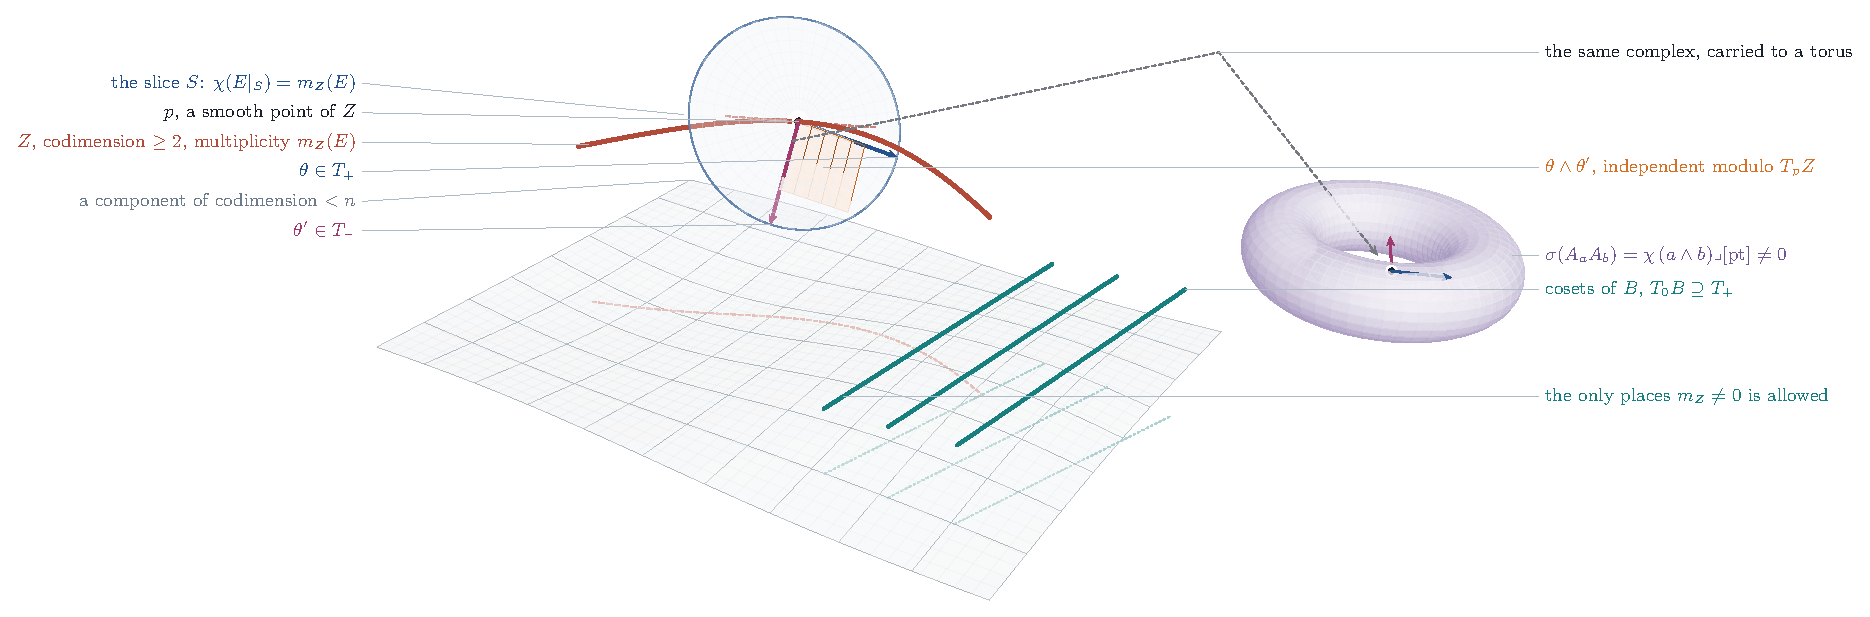
\includegraphics[width=\textwidth]{fig_support}
\caption{The proof of \Cref{thm:p2support}. The grey sheet stands for a
component of the support of codimension less than $n$, which the theorem
forces to exist; the clay curve $Z$ for a component of codimension at least
two. At a smooth point $p$ of $Z$ the directions $\theta\in T_{+}$ and
$\theta'\in T_{-}$ span the slice $S$, transverse to $Z$, on which $E$ restricts
to a complex of finite length with Euler characteristic $m_{Z}(E)$; the amber
parallelogram is the bivector $\theta\wedge\theta'$, independent modulo
$T_{p}Z$. Carried to a torus of the same dimension, the product of the two
jet classes is seen by the semiregularity map as $m_{Z}(E)$ times the class of
a point contracted with the bivector, which is not zero, so $m_{Z}(E)=0$ or
the bivector degenerates. The teal lines are cosets of an abelian subvariety
$B$ tangent to $T_{+}$, the only components of codimension at least two on
which a nonzero multiplicity survives. The scene is schematic in the
dimensions and exact in the incidences.}
\label{fig:support}
\end{figure}

\subsection{Indecomposability and endomorphisms}

The numerical criterion of \Cref{thm:p2numerical} fixes one number,
$\dim\Ext^{2}(E,E)$. Together with Serre duality, the lower bounds of
\Cref{cor:hhfactor} in the other degrees and the Hodge--Riemann relations for
the Weil class, it fixes a good deal more: the object that carries the class
can be taken indecomposable, and it has at least three linearly independent
endomorphisms at $n=2$ and, granting the compatibility of
\Cref{cor:hhfactor}(iii), at $n=3$, the first case in which the criterion
is needed at a nontrivial discriminant.

\begin{theorem}[The shape of an object meeting the criterion]
\label{thm:p2endo}
Let $A$, $\omega$ and $E$ be as in \Cref{thm:p2numerical}, so that
$\ch(E)=N\omega$ with $N\ne0$ and no other component, and suppose that
$\dim\Ext^{2}(E,E)=2n(2n-1)$. Write $e_{k}=\dim\Ext^{k}(E,E)$.
\begin{enumerate}[label=\textup{(\roman*)},leftmargin=2.6em,itemsep=2pt]
\item $\chi(E,E)=\sum_{k}(-1)^{k}e_{k}=(-1)^{n}N^{2}\int_{A}\omega^{2}$, and
  this number is positive.
\item $E\cong E_{0}\oplus E'$ with $E_{0}$ indecomposable,
  $\ch(E_{0})=\ch(E)$, $\dim\Ext^{2}(E_{0},E_{0})=2n(2n-1)$, $\ch(E')=0$ and
  $\Ext^{2}(E_{0},E')=\Ext^{2}(E',E_{0})=\Ext^{2}(E',E')=0$. So $E_{0}$ meets
  the criterion as well.
\item If $E$ is indecomposable, then $\End(E)=\CC\cdot\id\oplus J$ with $J$
  the nilpotent radical, every $f\in J$ annihilates $\Ext^{2}(E,E)$ and
  $\Ext^{2n-2}(E,E)$ under the Yoneda product, and
  $\operatorname{ev}_{E}(\bigwedge^{2n}P)=\operatorname{ev}_{E}(\bigwedge^{2n}Q)$
  is a single line in $\Ext^{2n}(E,E)$. If moreover $e_{1}=4n$, then $J$
  annihilates $\Ext^{1}(E,E)$ as well.
\item If $n=2$ or $n=3$, then
  \[
    \dim\End(E)\;\ge\;2+\tfrac12\,\chi(E,E)\;>\;2,
  \]
  so $E$ has at least three linearly independent endomorphisms, and at
  $n=3$ also $e_{1}\le e_{0}+9$. In particular no simple object meets the
  criterion: no stable sheaf, no complex with $\End=\CC$, and no image of one
  under an autoequivalence of $D^{b}(A)$; and an indecomposable object that
  meets it has a nonzero nilpotent endomorphism. The smallest profiles
  $(e_{0},\dots,e_{2n})$ that the constraints allow are $(3,8,12,8,3)$ at
  $n=2$, with $\chi=2$, and $(3,12,30,40,30,12,3)$ and $(3,12,30,41,30,12,3)$
  at $n=3$, with $\chi=2$ and $\chi=1$.
\end{enumerate}
Parts (i) and (ii), and part (iv) at $n=2$, use the compatibility
$\sigma_{E}\circ\operatorname{ev}_{E}=(\,\cdot\,)\lrcorner\ch(E)$ of
\Cref{setup:hh} in degree two only, as \Cref{thm:p2numerical} does. Part
(iii), and part (iv) at $n=3$, use it in the further degrees in which
\Cref{cor:hhfactor}(iii) grants it: $2n-2$ and $2n$ for (iii), and three for
(iv).
\end{theorem}

\begin{proof}
(i) The Todd class of $A$ is trivial, so the Riemann--Roch theorem gives
$\chi(E,E)=\int_{A}\ch(E)^{\vee}\ch(E)$, and $\ch(E)^{\vee}=(-1)^{n}N\omega$
since $\omega$ has degree $2n$. The polarisation pairs $V_{+}$ only with
$V_{-}$ (see \Cref{fig:tangent}), so its class $\theta$ lies in
$V_{+}\otimes V_{-}$ and $\theta\wedge\alpha_{\pm}=0$, because $\alpha_{\pm}$
spans the top exterior power of $V_{\pm}$. So $\omega$ is a nonzero rational
primitive class of type $(n,n)$ in the middle degree, and the Hodge--Riemann
relations give $(-1)^{n(2n-1)}\int_{A}\omega^{2}>0$, where
$(-1)^{n(2n-1)}=(-1)^{n}$.

(ii) The category $D^{b}(A)$ has finite dimensional morphism spaces and split
idempotents, so $E=\bigoplus_{i}E_{i}$ with each $E_{i}$ indecomposable. The
evaluation map and the semiregularity map are compatible with direct sums,
and by \Cref{thm:p2numerical}(i) the kernel of $\operatorname{ev}_{E}$ in
degree two is $P\wedge Q$; so $\operatorname{ev}_{E_{i}}(P\wedge Q)=0$ and,
composing with $\sigma_{E_{i}}$, $(P\wedge Q)\lrcorner\ch(E_{i})=0$ for every
$i$. We claim that the only classes of Hodge type killed by $P\wedge Q$ are
those of $\CC\alpha_{+}\oplus\CC\alpha_{-}$. Write
$H^{*}(A,\CC)=\bigwedge^{*}(A_{+}\oplus B_{+}\oplus A_{-}\oplus B_{-})$ with
$A_{\pm}=V_{\pm}^{1,0}$ and $B_{\pm}=V_{\pm}^{0,1}$, and grade it by the four
degrees $(i,j,k,l)$. As in \Cref{setup:hh}, $P$ acts by wedging with $B_{+}$
and contracting $A_{-}$, and $Q$ by wedging with $B_{-}$ and contracting
$A_{+}$, so $P\wedge Q$ is spanned by four kinds of operators, each of which
shifts the four degrees by a fixed amount: wedging with $b_{+}\wedge b_{-}$
kills a component of degree $(i,j,k,l)$ for all choices exactly when $j=n$ or
$l=n$; wedging with $b_{+}$ after contracting $a_{+}$, exactly when $i=0$ or
$j=n$; contracting $a_{-}$ and wedging with $b_{-}$, exactly when $k=0$ or
$l=n$; and contracting $a_{-}$ and $a_{+}$, exactly when $i=0$ or $k=0$. Each
of these is a statement about a tensor product of maps that are injective
unless the degree in question is extreme. A class of type $(p,p)$ has
$i+k=j+l=p$ in every component. If $j=n$, then $l=n$ would force $i=k=n$,
against the fourth condition, so $l<n$ and the third condition gives $k=0$;
hence $i=n+l$, so $i=n$ and $l=0$: the component lies in
$\bigwedge^{n}A_{+}\otimes\bigwedge^{n}B_{+}=\CC\alpha_{+}$. If $j<n$, the
first two conditions give $l=n$ and $i=0$, hence $k=n$ and $j=0$: the
component lies in $\CC\alpha_{-}$. This proves the claim. Since $\ch(E_{i})$ is a rational class of
Hodge type killed by $P\wedge Q$, it lies on the rational Weil plane, and
when it is nonzero \Cref{cor:hhfactor}(i) gives
$\dim\Ext^{2}(E_{i},E_{i})\ge2n(2n-1)$, a nonzero rational Weil class having
both coefficients $a$ and $b$ nonzero. As
$\Ext^{2}(E,E)=\bigoplus_{i,j}\Ext^{2}(E_{i},E_{j})$ has dimension
$2n(2n-1)$ and $\sum_{i}\ch(E_{i})=N\omega\ne0$, exactly one summand $E_{0}$
has nonzero Chern character and every other block of $\Ext^{2}$ vanishes.

(iii) An indecomposable object of a category with finite dimensional
morphism spaces and split idempotents has a local endomorphism ring, so
$\End(E)=\CC\cdot\id\oplus J$ with $J$ nilpotent. By
\Cref{thm:p2numerical}(i), $\operatorname{ev}_{E}$ maps
$\bigwedge^{2}P\oplus\bigwedge^{2}Q$ isomorphically onto $\Ext^{2}(E,E)$.
By Serre duality $e_{2n-2}=e_{2}$, and contraction with $\omega$ is injective
on $\bigwedge^{2n-2}P\oplus\bigwedge^{2n-2}Q$ by \Cref{thm:hhsplitting}(iv),
since $2n-2\ne2n$; so, with the compatibility in
degree $2n-2$, $\operatorname{ev}_{E}$ maps that space isomorphically onto
$\Ext^{2n-2}(E,E)$. In degree $2n$ the semiregularity map is the trace, since
$H^{q+2n}(\Omega^{q}_{A})=0$ for $q>0$, so
$\operatorname{tr}\operatorname{ev}_{E}(\xi)$ is the $H^{0,2n}$ component of
$\xi\lrcorner\ch(E)$; for the generators $\pi_{P}$, $\pi_{Q}$ of
$\bigwedge^{2n}P$ and $\bigwedge^{2n}Q$ it is $Nc_{P}$ and $Nc_{Q}$ with
$c_{P}c_{Q}\ne0$. Indeed $\pi_{P}$ wedges with a basis of $B_{+}$ and contracts
a basis of $A_{-}$, so it kills $\alpha_{+}$, whose factor $\bigwedge^{n}B_{+}$
is already full, and carries $\alpha_{-}$ to $\pm$ the generator
$\bigwedge^{n}B_{+}\wedge\bigwedge^{n}B_{-}$ of $H^{0,2n}$; so $c_{P}=\pm b$
and likewise $c_{Q}=\pm a$, both nonzero. For $f\in\End(E)$ and
$x\in\bigwedge^{2}P\oplus\bigwedge^{2}Q$ write
$f\cdot\operatorname{ev}_{E}(x)=\operatorname{ev}_{E}(\varphi_{f}(x))$; then
$f\mapsto\varphi_{f}$ is a homomorphism of algebras. Let $x\in\bigwedge^{2}P$
and $y\in\bigwedge^{2n-2}P$, and write $x\wedge y=\beta(x,y)\pi_{P}$. Since
$\operatorname{ev}_{E}$ is a ring map that kills the ideal generated by
$P\wedge Q$,
\[
  \beta(x,y)\operatorname{tr}\bigl(f\operatorname{ev}_{E}(\pi_{P})\bigr)
  =\operatorname{tr}\bigl(f\operatorname{ev}_{E}(x)\operatorname{ev}_{E}(y)\bigr)
  =\operatorname{tr}\operatorname{ev}_{E}\bigl(\varphi_{f}(x)\wedge y\bigr)
  =Nc_{P}\,\beta\bigl(\varphi_{f}(x)_{P},y\bigr),
\]
and the pairing $\beta$ is perfect, so $\varphi_{f}(x)_{P}=\mu_{f}x$ with
$\mu_{f}=\operatorname{tr}(f\operatorname{ev}_{E}(\pi_{P}))/Nc_{P}$. The same
computation with $y\in\bigwedge^{2n-2}Q$, where $x\wedge y$ lies in the ideal
generated by $P\wedge Q$, gives $\varphi_{f}(x)_{Q}=0$. So $f$ acts on
$\operatorname{ev}_{E}(\bigwedge^{2}P)$ by a scalar $\mu_{f}$, and in the same
way on $\operatorname{ev}_{E}(\bigwedge^{2}Q)$ by a scalar $\nu_{f}$; $\mu$ and
$\nu$ are characters of $\End(E)$ and vanish on $J$. So $J$ kills
$\Ext^{2}(E,E)$, on both sides because $\operatorname{ev}_{E}$ lands in the
graded centre, and the same argument with the roles of the two degrees
exchanged shows that it kills $\Ext^{2n-2}(E,E)$. In particular
$\operatorname{tr}(f\operatorname{ev}_{E}(\pi_{P}))=\mu_{f}Nc_{P}=0$ for
$f\in J$, so $\operatorname{ev}_{E}(\pi_{P})$ and, likewise,
$\operatorname{ev}_{E}(\pi_{Q})$ lie in the annihilator of $J$ under the
perfect pairing of $\End(E)$ with $\Ext^{2n}(E,E)$. That annihilator is a
line, $J$ having codimension one, and both elements are nonzero, their traces
being $Nc_{P}$ and $Nc_{Q}$; so they span the same line. Finally, if
$e_{1}=4n$ then $\Ext^{1}(E,E)=\operatorname{ev}_{E}(HH^{1})$, because
$\operatorname{ev}_{E}$ is injective on $HH^{1}$, as shown in (iv). For
$f\in J$ and $h\in HH^{1}$ write $f\operatorname{ev}_{E}(h)=
\operatorname{ev}_{E}(h')$; then
$\operatorname{ev}_{E}(h'\wedge h'')=f\operatorname{ev}_{E}(h\wedge h'')=0$ for
every $h''\in HH^{1}$, so $h'\wedge HH^{1}\subseteq P\wedge Q$, which forces
$h'=0$ since $\dim P=\dim Q\ge2$.

(iv) By Serre duality $e_{k}=e_{2n-k}$. The map $\operatorname{ev}_{E}$ is
injective on $HH^{1}$ using degree two alone: if $\operatorname{ev}_{E}(h)=0$
then $\operatorname{ev}_{E}(h\wedge h')=0$ for every $h'$, so
$h\wedge HH^{1}\subseteq\Ann_{HH^{2}}(\omega)=P\wedge Q$, and $h=0$ as in
(iii). So $e_{1}\ge4n$, and \Cref{cor:hhfactor}(iii) gives
$e_{3}\ge2\binom{6}{3}=40$ at $n=3$. At $n=2$ the Euler
characteristic is $2e_{0}-2e_{1}+12$, and at $n=3$ it is
$2e_{0}-2e_{1}+60-e_{3}$. So $2e_{0}=\chi+2e_{1}-12\ge\chi+4$ at $n=2$, and
$2e_{0}=\chi+2e_{1}+e_{3}-60\ge\chi+4$ at $n=3$, where also
$e_{1}=e_{0}+30-\frac12(\chi+e_{3})\le e_{0}+9$. With (i) this gives the
bound. An autoequivalence preserves $\End$, and a stable sheaf is simple.
An indecomposable object with $\dim\End\ge3$ has $J\ne0$. For the smallest
profiles take $e_{0}=3$. At $n=2$, $\chi$ is even and positive, so
$2e_{1}=18-\chi\le16$, and $e_{1}\ge8$ forces $e_{1}=8$ and $\chi=2$. At
$n=3$, $2e_{1}+e_{3}=66-\chi\le65$ with $e_{1}\ge12$ and $e_{3}\ge40$
forces $e_{1}=12$ and $e_{3}\in\{40,41\}$, with $\chi=2$ and $\chi=1$.
\end{proof}

\begin{remark}[Objects excluded by the shape]\label{rem:p2endo}
\Cref{thm:p2endo} gives necessary conditions only, and their effect is to
exclude the objects one would construct first. Line bundles, semi-homogeneous
bundles, skyscraper sheaves, stable sheaves and their Fourier--Mukai
transforms are simple, and direct sums of them are excluded by (ii) together
with \Cref{thm:nosum}. At $n=3$, granting the compatibility of
\Cref{cor:hhfactor}(iii), the shape allowed is an indecomposable object
with a local endomorphism algebra of dimension at least three whose radical
kills $\Ext^{2}$ and $\Ext^{4}$ and pairs to zero with the line
$\operatorname{ev}_{E}(\bigwedge^{6}P)$. The smallest conceivable one has
$\Hom(E,E)$ of dimension three, $\Ext^{1}(E,E)$ equal to the image of
$HH^{1}(A)$, of dimension twelve and killed by the radical, and
$\Ext^{3}(E,E)$ of dimension forty or forty-one. Iterated self-extensions and
thickenings are the natural objects with nilpotent endomorphisms, but an
extension of a simple object $F$ by itself has $\ch=2\ch(F)$, so $F$ would
already have to carry the class, and the question returns one level down.
For $n\ge4$ write $e_{k}=2\binom{2n}{k}+\delta_{k}$ for $1\le k\le2n-1$,
with $\delta_{k}\ge0$ and $\delta_{2}=\delta_{2n-2}=0$. Since
$\sum_{k=1}^{2n-1}(-1)^{k}\binom{2n}{k}=-2$, the Euler characteristic is
$2e_{0}-4+\sum_{k}(-1)^{k}\delta_{k}$, and an excess $\delta_{k}$ in an even
degree $4\le k\le2n-4$ can make it positive with $e_{0}=1$; so the bound on
$\End$ disappears. By
\Cref{thm:p2false} none of these shapes is realised.
\end{remark}


\part{Semiregularity and secant objects}\label{part:semiregularity}
\section{The semiregularity criterion in its pure and polarised forms}\label{sec:polarised}

\subsection{Weil tori and the pure form of the criterion}

The object $E$ of \Cref{sec:propagation} has Chern character exactly
$N\omega$. For such an object, injectivity of $\sigma_{E}$ would make $E$
extend along every $K$-linear deformation of $A$ (\Cref{thm:p2forces}(ii)). These
deformations reach non-algebraic tori, on which the Weil class is a Hodge
class but not a Chern class of any coherent sheaf. This settles the pure form
of the criterion, negatively, in every dimension.

\begin{setupenv}[Weil tori]\label{setup:weiltori}
Let $A$ be an abelian $2n$-fold of $(K,-1,n)$-Weil type, $V=H^{1}(A,\QQ)$ with
its action of $K$, and $V\otimes\CC=V_{+}\oplus V_{-}$ the two eigenspaces,
each of dimension $2n$. For complementary $n$-dimensional subspaces
$X,Y\subset V_{+}$ the subspace $X\oplus\bbar{Y}$ of $V\otimes\CC$ is the
space of holomorphic $1$-forms of a complex structure on the real torus
underlying $A$; call the resulting complex torus $T_{X,Y}$. On $T_{X,Y}$ the
field $K$ acts with signature $(n,n)$, so $T_{X,Y}$ is a Weil torus in the
sense of \cite{Voi02b}, and every complex structure on that real torus
commuting with $K$ and of signature $(n,n)$ arises in this way. The pairs
$(X,Y)$ form a connected complex manifold $S$ of dimension $2n^{2}$,
containing the point of $A$; the polarised Weil family is the submanifold of
dimension $n^{2}$ on which the polarisation of $A$ is of type $(1,1)$, and the
tangent space of $S$ is the space $\Hom_{K}(H^{1,0},H^{0,1})$ of $K$-linear
first order deformations in \Cref{thm:p2forces}(i). Since
$\alpha_{+}$ spans $\bigwedge^{2n}V_{+}=\bigwedge^{n}X\otimes\bigwedge^{n}Y$
and $X$ is holomorphic while $Y$ is antiholomorphic, the Weil classes are of
type $(n,n)$ on every $T_{X,Y}$. We say that a property holds for a very
general member of $S$ if it holds outside a countable union of proper
analytic subsets.
\end{setupenv}

\begin{lemma}[The Hodge classes of a very general Weil torus]
\label{lem:weiltorushodge}
For a very general member $T$ of $S$, $\Hdg^{k}(T)=0$ for
$1\le k\le2n-1$, $k\ne n$, and $\Hdg^{n}(T)$ is the rational Weil plane.
\end{lemma}

\begin{proof}
There are countably many rational classes, and the Hodge locus of each is an
analytic subset of the connected manifold $S$; so a rational class that is of
Hodge type at a very general member is of Hodge type on all of $S$.
Let $G=\Res_{K/\QQ}\mathrm{GL}_{2n}$ be the group of $K$-linear automorphisms
of $V$. Its real points act transitively on $S$, since
$\mathrm{GL}(V_{+})$ acts transitively on pairs of complementary subspaces.
The Mumford--Tate group $M$ of a very general member lies in $G$, since $K$
acts by endomorphisms of every member, and it contains the Mumford--Tate group
of every member, whose Hodge classes include those of the very general one.
So the real Lie algebra of $M$ contains the complex structure $J_{s}$ of every
member, which is the derivative of its Hodge cocharacter, and therefore
contains the $\mathrm{Ad}\,G(\RR)$-span of one $J_{s}$. This span is an ideal of
$\mathfrak{g}_{\RR}=\mathfrak{gl}_{2n}(\CC)$ containing the non-central
element $J_{s}$, which acts on $V_{+}$ by $i$ on $X$ and by $-i$ on $Y$; hence
it contains $\mathfrak{sl}_{2n}(\CC)$, and $M$ contains
$G^{\mathrm{der}}=\Res_{K/\QQ}\mathrm{SL}_{2n}$. Over $\CC$ this is
$\mathrm{SL}(V_{+})\times\mathrm{SL}(V_{-})$ acting on
$\bigwedge^{*}(V_{+}\oplus V_{-})=\bigwedge^{*}V_{+}\otimes\bigwedge^{*}V_{-}$,
whose invariants are spanned by $1$, $\alpha_{+}$, $\alpha_{-}$ and
$\alpha_{+}\alpha_{-}$. Hodge classes are invariant under $M$, which gives
the statement.
\end{proof}

\begin{lemma}[A very general Weil torus has no subvarieties]
\label{lem:weiltorussubsets}
A very general member $T$ of $S$ has no analytic subsets other than finite
sets and $T$ itself.
\end{lemma}

\begin{proof}
Let $Z\subset T$ be an irreducible analytic subset of codimension $c$ with
$0<c<2n$. For every K\"ahler class $\kappa$ the class $[Z]$ satisfies
$\int_{T}[Z]\,\kappa^{2n-c}=\int_{Z}\kappa^{2n-c}>0$, so $[Z]$ is a nonzero
Hodge class of degree $2c$. By \Cref{lem:weiltorushodge} this forces $c=n$ and
$[Z]$ into the Weil plane. Take for $\kappa_{0}$ the class of a positive
definite hermitian form that is block diagonal for the splitting
$H^{1,0}=X\oplus\bbar{Y}$. Its blocks lie in $X\otimes\bbar{X}$ and
$\bbar{Y}\otimes Y$, both inside $V_{+}\otimes V_{-}$, so every power of
$\kappa_{0}$ has a factor from $V_{+}$ and a factor from $V_{-}$ in each term,
and $\alpha_{\pm}\wedge\kappa_{0}^{n}=0$ because $\alpha_{\pm}$ spans the top
exterior power of $V_{\pm}$. So
$\int_{T}[Z]\,\kappa_{0}^{n}=0$, which is impossible.
\end{proof}

\begin{proposition}[Coherent sheaves on a very general Weil torus]
\label{prop:weiltorussheaves}
Let $n\ge2$ and let $T$ be a very general member of $S$. Every coherent
analytic sheaf $F$ on $T$ has $\ch_{k}(F)=0$ in $H^{2k}(T,\QQ)$ for
$1\le k\le2n-1$. For $n=2$ this is Voisin's theorem that every coherent sheaf
on a general Weil torus of dimension four has $c_{2}(F)=0$
\cite[Theorem~10]{Voi02b}, whose proof we follow.
\end{proposition}

\begin{proof}
Chern classes of coherent sheaves on $T$ exist in rational Deligne
cohomology, extend those of bundles and are additive \cite{Gri10}, so they
are Hodge classes. By \Cref{lem:weiltorussubsets} the torsion of $F$, the locus where the
torsion-free quotient is not locally free, and the cokernel of the map from
that quotient to its reflexive hull are all supported on finite sets, and a
sheaf supported on a finite set has Chern character in the top degree only. So
it suffices to treat a reflexive sheaf $G$. Every coherent sheaf on $T$ has
$c_{1}=0$, since $\Hdg^{1}(T)=0$ (\Cref{lem:weiltorushodge}); so every
torsion-free sheaf has slope zero for every K\"ahler class, and a torsion-free
sheaf is stable for one K\"ahler class exactly when it has no saturated
subsheaf of intermediate rank, which does not depend on the class. A
Jordan--H\"older filtration of $G$ therefore has stable torsion-free factors
$Q_{j}$, stable for every K\"ahler class, and $\ch(G)=\sum_{j}\ch(Q_{j})$.
By the theorem of Bando and Siu \cite{BS94} the stable reflexive sheaf
$Q_{j}^{**}$ carries an admissible Hermite--Einstein metric for every K\"ahler
class $\kappa$ and satisfies
$\int_{T}\bigl(2rc_{2}-(r-1)c_{1}^{2}\bigr)(Q_{j}^{**})\,\kappa^{2n-2}\ge0$,
with equality exactly when $Q_{j}^{**}$ is a projectively flat vector bundle.
Here $c_{1}=0$ and $c_{2}(Q_{j}^{**})\in\Hdg^{2}(T)$. For $n\ge3$ that group is
zero; for $n=2$ it is the Weil plane, and then
$\int_{T}c_{2}(Q_{j}^{**})\,\kappa_{0}^{2}=0$ for the class $\kappa_{0}$ of
the proof of \Cref{lem:weiltorussubsets}. In either case equality holds for
some $\kappa$, so $Q_{j}^{**}$ is a projectively flat bundle with $c_{1}=0$,
hence flat, and its rational Chern classes of positive degree vanish. Since
$Q_{j}$ and $Q_{j}^{**}$ differ only on a finite set, $\ch_{k}(Q_{j})=0$ for
$1\le k\le2n-1$, and the same holds for $G$ and for $F$.
\end{proof}

\begin{theorem}[The pure form of the criterion is never met]
\label{thm:p2false}
Let $n\ge2$, let $A$ be an abelian $2n$-fold of $(K,-1,n)$-Weil type, $\omega$
a nonzero rational Weil class, and $E$ a perfect complex on $A$ with
$\ch(E)=N\omega$, $N\ne0$, and no other component. Then $\sigma_{E}$ is not
injective. In particular $\dim\Ext^{2}(E,E)>2n(2n-1)$, the hypotheses of
\Cref{thm:semiregclosure} and \Cref{thm:p2numerical}(iii) are satisfied by no
object at any member of any Weil family of an imaginary quadratic field, and
the propagation statement \textup{(P2)} of \Cref{rem:tworemain}, in the form
stated there, is false.
\end{theorem}

\begin{proof}
Suppose that $\sigma_{E}$ is injective. Since $A$ is projective, $E$ is isomorphic to
a bounded complex $E^{\bullet}$ of holomorphic vector bundles. The class
$N\omega$ is of Hodge type on every member of $S$ (\Cref{setup:weiltori}), so
by the theorem of Buchweitz and Flenner in Pridham's form (\Cref{thm:BF},
\cite{BF03,Pri24}), every obstruction to extending $E$ along an
Artinian deformation of $A$ inside $S$ vanishes, exactly as in the proof of
\Cref{thm:semiregclosure}. The deformations of the complex structure inside
$S$ together with those of the holomorphic structures and differentials of
$E^{\bullet}$ are governed by a differential graded Lie algebra of Dolbeault
type with finite dimensional cohomology, and Kuranishi's method
\cite{Kur65}, in the form of \cite[Sections~2--3]{GM88}, gives an analytic
germ $(M,m_{0})$ with a morphism $\pi\colon(M,m_{0})\to(S,s_{0})$ and a
complex of holomorphic vector bundles on the pulled back family of tori
deforming $E^{\bullet}$, whose completion is a hull of the formal deformation
functor. The vanishing of the obstructions says that $\pi$ is formally
smooth, hence smooth, so its image contains a neighbourhood $U$ of $s_{0}$.
Thus every member $T_{s}$ with $s\in U$ carries a bounded complex of
holomorphic vector bundles $E_{s}^{\bullet}$ whose Chern character is the
parallel transport of $N\omega$. Choose $s\in U$ very general. By
\Cref{prop:weiltorussheaves},
$\ch_{n}(E_{s})=\sum_{i}(-1)^{i}\ch_{n}(E_{s}^{i})=0$, while it is the
transport of $N\omega$, which is not zero. This contradiction proves that
$\sigma_{E}$ is not injective. The argument uses only that $\ch(E)$ is of
Hodge type on every member of $S$, so it applies verbatim when $\ch(E)-N\omega$
has components in degrees $0$ and $4n$ as well. The remaining statements
follow, since $\dim\Ext^{2}(E,E)\ge2n(2n-1)$ by \Cref{cor:hhfactor}(i),
and equality forces $\sigma_{E}$ to be injective by
\Cref{thm:p2numerical}(i).
\end{proof}

\begin{remark}[The polarised criterion]\label{rem:p2prime}
\Cref{thm:p2false} turns \Cref{thm:p2forces}(ii) from a constraint into a
contradiction: an object that extends along every $K$-linear deformation of
$A$ reaches non-algebraic tori, where the Weil class is a Hodge class but not
a Chern class. The results that describe such an object,
\Cref{thm:p2forces}, \Cref{cor:hhfactor}(ii)--(iii), \Cref{thm:p2numerical},
\Cref{thm:p2support}, \Cref{thm:nosum} and \Cref{thm:p2endo}, remain true as
implications, but they are vacuous: no object satisfies their hypotheses.
They record what the pure form asks of an object, and
\Cref{rem:p2primesurvive} says which of them extend to the polarised form
defined next.

The obstruction does not reach a Chern character with a component that is of
Hodge type on the polarised family and not beyond it, unless a twist removes
that component. Call
\textup{(P2$'$)} the statement that at one base point of each Weil family
some perfect complex $E$ with
\[
  \ch(E)=N\omega_{1}+\sum_{k}c_{k}\,\theta^{k},\qquad N\ne0,\ c_{k}\in\QQ,
\]
$\theta$ the polarisation, has injective semiregularity map. The proof of
\Cref{thm:semiregclosure} applies to it word for word, with the deformation
taken over the polarised family, along which $\ch(E)$ stays of Hodge type:
at a member $A_{s}$ it produces $\ch_{n}(E_{s})=N\omega_{1}+c_{n}\theta^{n}$
algebraic, and $\theta^{n}$ is algebraic, so $\omega_{1}$ is. The form above
is already the most general one allowed by the subring generated by $\theta$
and the Weil classes: a Weil class is primitive, so $\theta\omega_{1}=0$ and
that subring is spanned by the powers of $\theta$ and the Weil plane.
\Cref{thm:p2false} excludes directly a Chern character that remains of Hodge
type on all of $S$, which by \Cref{lem:weiltorushodge} is a multiple of the
Weil class plus terms in degrees $0$ and $4n$, and after a line bundle twist
the characters $c\,e^{t\theta}+N\omega_{1}+c'\theta^{2n}$ with $t\theta$
integral (\Cref{thm:p2primenumber}(v)). For every other polarised character
with some $c_{k}\ne0$, $1\le k\le2n-1$, the component of the Hodge locus of
$\ch(E)$ through $A$ is the polarised family itself, whose members are
abelian varieties, so nothing forces $E$ onto non-algebraic tori and the
argument cannot be run on $E$ (\Cref{prop:p2primelocus}); the one exception is
a ratio at $n=2$ at which the locus is five-dimensional
(\Cref{rem:p2primeexceptional}). The semiregular objects in Markman's
proofs for abelian fourfolds and for the sixfolds of trivial discriminant
\cite{Mar25a,Mar25b} are not of the pure form: their Chern characters are not
multiples of a Weil class, and they are deformed only along families on which
those characters stay of Hodge type, and nothing below depends on whether
they have exactly the form above. From here on, in
\Cref{cor:fourremain}, \Cref{thm:closure} and the frontier of
\Cref{sec:scope}, \textup{(P2)} is read in this polarised form. The
annihilator computations of \Cref{sec:propagation} assume that $\ch(E)$ is a
pure Weil class; the next subsection carries them out for a Chern character
with components in every even degree (\Cref{thm:p2primenumber},
\Cref{prop:p2primeprofile}, \Cref{prop:p2primelocus}).

The same obstruction does not reach the Mumford target of
\Cref{ssec:mumfordrigid}. The exceptional classes there are rigid: their Hodge
locus among all complex tori is the Mumford curve (\Cref{thm:mumfordrigid},
\Cref{prop:notwistor}), so a semiregular complex with Chern character
$N\omega$ on the square of a Mumford fourfold would only have to deform along
the curve, whose members are all algebraic.
\end{remark}

\begin{remark}[Two finite statements]
\label{rem:tworemain}
After \Cref{thm:degreebound} and \Cref{thm:semiregclosure} the Hodge
conjecture for abelian varieties of Weil type follows from either of the
following, each of which is a statement about explicit finite data and neither
of which mentions a general point. The first is settled by
\Cref{thm:p1equivalent}, and we record it because it is the form in which the
question first presents itself. The second is false as stated here
(\Cref{thm:p2false}), and its polarised form, \textup{(P2$'$)} of
\Cref{rem:p2prime}, is computed in closed form below.

\begin{enumerate}[label=\textup{(P\arabic*)},leftmargin=*]
\item \emph{A bound.} At every point of the orbit $G(\QQ)\cdot s_{0}$ the
  class $\omega$ is represented by a cycle whose Hilbert data comes from one
  finite set. \Cref{thm:p1forces} shows that the transport of the base cycle
  does not satisfy this, for any cycle whose components have finite
  stabiliser, and \Cref{thm:p1equivalent} shows that, read on an arbitrary
  representative, the statement is equivalent to $\mathbf{W}(K,n,\delta)$
  itself. It is therefore a reformulation of the conjecture for the family,
  and we record it as such rather than as a criterion.
\item \emph{A rank.} The semiregularity map of a perfect complex with the
  Chern character of \Cref{prop:ktheory} at one base point is injective.
  In this form the statement is false (\Cref{thm:p2false}); its polarised
  form, in \Cref{rem:p2prime}, allows the Chern character to carry powers of
  the polarisation, and what follows records what the pure form asks. The
  source of the map is $\Ext^{2}(E,E)$ for a single object, and its target
  has dimension $\sum_{q}h^{q,q+2}(A_{0})=\binom{4n}{2n-2}$, computed in
  \Cref{prop:target}. So the target is large, which is the direction that
  helps, and the question is the rank of the map. Full rank would force the
  following (\Cref{thm:p2forces}): the evaluation map of
  Hochschild cohomology must vanish on the $4n^{2}$-dimensional annihilator of
  the Weil class, so $E$ must be killed by the mixed block of $H^{0,2}$, must
  extend along every $K$-linear deformation, must have all products of
  transverse translation classes zero, and must have no endomorphism of
  nonzero trace; and at a base point with no abelian subvariety tangent to an
  eigenspace it can be a locally free sheaf on no smooth germ of its support
  of codimension at least two (\Cref{cor:p2shape}). The representative that
  the construction supplies, a virtual sum of line bundles, fails at the first
  of these (\Cref{prop:concentrated}), and any representative that is a
  sheaf fails at the last. \Cref{thm:hhsplitting} identifies that
  annihilator as the mixed part of a splitting $HH^{1}=P\oplus Q$ into the
  annihilators of the two conjugate pieces of the class, and
  \Cref{cor:hhfactor} draws the consequence: the whole Hochschild action of
  $E$ factors through a ring of dimension $2^{2n+1}-1$ inside one of
  dimension $2^{4n}$, while $\dim\Ext^{2}(E,E)\ge2n(2n-1)$ for every
  representative, semiregular or not. \Cref{thm:p2numerical} turns the rank
  condition into that number: equality suffices. \Cref{thm:p2support} locates
  the support: at every member it has a component of codimension less than
  $n$, so no complex carried by a cycle representing $\omega$ can serve, and
  at a general member every component of codimension at least two has
  multiplicity zero.
  \Cref{thm:p2endo} fixes its shape: an indecomposable summand carries the
  class and meets the criterion alone, and at $n=2$, and at $n=3$ granting
  the compatibility of \Cref{cor:hhfactor}(iii), it has at least three
  independent endomorphisms, so no simple object serves.
\end{enumerate}

Neither statement is the variational Hodge conjecture: (P1) says nothing
about deformations, and (P2) is an infinitesimal statement at one point, the
global propagation being supplied by \Cref{thm:closedlocus}, which is what
\Cref{rem:variational} identifies as missing. Nor is either implied by the
results of \Cref{ssec:everyfamily}: the base points and the cycles are
constructed there, and (P1) and (P2) are questions about those same cycles
that the construction does not answer. In the forms stated here both are
settled: (P1) is equivalent to its conclusion, and (P2) is false. Its
polarised form in \Cref{rem:p2prime} is the criterion that the rest of this
section computes.
\end{remark}

\subsection{The polarised criterion in closed form}

The annihilator computations of \Cref{sec:propagation} assume that $\ch(E)$
is a pure Weil class, as \Cref{rem:p2prime} notes. This subsection carries
them out for a Chern character with components in every even degree. In
degree two the answer is complete and holds for every $n$; in the other
degrees it is a closed formula, with one correction term in the middle
degree. The same computation gives the Hodge locus of the character,
and with it the list of the obstructions of this paper that apply to
polarised characters (\Cref{prop:p2primelocus}, \Cref{rem:p2primesurvive}).
None of this constructs an object or decides whether one exists. It gives,
for each shape of Chern character, the number that $\dim\Ext^{2}(E,E)$ has
to reach and the exact kernel that $\operatorname{ev}_{E}$ must then have,
which is the form in which a candidate can be tested.

\begin{setupenv}[Polarised characters]\label{setup:p2prime}
Let $A$ be an abelian $2n$-fold of $(K,-1,n)$-Weil type, $n\ge2$, with
polarisation $\theta$, and let $\omega=u\alpha_{+}+\bbar u\,\alpha_{-}$ be a
nonzero real class on the Weil line, in the notation of \Cref{thm:p2forces}.
For complex numbers $c_{0},\dots,c_{2n}$ put
\[
  p(\theta)=\sum_{k=0}^{2n}c_{k}\theta^{k},\qquad
  \gamma=\omega+p(\theta),\qquad \mu_{m}=m!\,c_{m},
\]
and let $\rho\in\{0,1,2,3\}$ be the rank of the $(2n-1)\times3$ Hankel matrix
$H=[\mu_{j+i}]$, $0\le j\le2n-2$, $0\le i\le2$. Write $r(\gamma)$ for the
rank of contraction $HT^{2}(A)\to H^{*}(A,\CC)$, $\xi\mapsto\xi\lrcorner\gamma$.
For $a<n\le b$, in the basis of \Cref{thm:hhsplitting} adapted to an
eigenbasis $e_{j}$ of $V_{+}$ and $f_{j}$ of $V_{-}$ with $e_{j},f_{j}$ of
type $(1,0)$ for $j<n$ and $j\ge n$ respectively, write
$z_{ab}=w(e_{b})w(f_{a})\in V_{+}^{0,1}\otimes V_{-}^{0,1}$,
$v^{1}_{ab}=w(e_{b})c(e_{a})$ and $v^{2}_{ab}=w(f_{a})c(f_{b})$ in
$H^{1}(T_{A})$, and $\pi_{ab}=c(e_{a})c(f_{b})\in T_{+}\otimes T_{-}$, where
$w$ is wedge product with a $(0,1)$ class and $c$ contraction of a $(1,0)$
class.
\end{setupenv}

The matrix $H$ is a catalecticant of the moment sequence
$\mu_{m}=m!\,c_{m}$. A nonzero vector $(x,\lambda,w)$ in its kernel is a
linear recurrence $x\mu_{j}+\lambda\mu_{j+1}+w\mu_{j+2}=0$ of order at most
two, so $\rho\le2$ says that the moments satisfy one, and the shapes of
\Cref{thm:p2primenumber}(ii) are its solutions, read off from the roots of
$wT^{2}+\lambda T+x$. For a Chern character,
$\gamma=N\omega_{1}+\sum_{k}c_{k}\theta^{k}$ with rational $c_{k}$, and $u$
is determined by $N\omega_{1}$. Since $\alpha_{\pm}^{2}=0$,
$\int_{A}\omega^{2}=2|u|^{2}\int_{A}\alpha_{+}\alpha_{-}$; scaling the
eigenbases so that $\int_{A}\alpha_{+}\alpha_{-}=(-1)^{n}\int_{A}\theta^{2n}/(2n)!$,
which is possible because the sign of $\int_{A}\alpha_{+}\alpha_{-}$ is
$(-1)^{n}$ by the Hodge--Riemann relations, one has
$|u|^{2}=(-1)^{n}\tfrac{(2n)!}{2}\int_{A}\omega^{2}\big/\!\int_{A}\theta^{2n}$.
The rank
$\rho$ does not change when
$\gamma$ is multiplied by $e^{t\theta}$, which acts on the moments by a
binomial transform, and $\omega e^{t\theta}=\omega$ because a Weil class is
primitive; so $\rho$ is an invariant of $\gamma$ up to twist.

\begin{theorem}[The polarised criterion as a number]\label{thm:p2primenumber}
In \Cref{setup:p2prime}:
\begin{enumerate}[label=\textup{(\roman*)},leftmargin=2.6em,itemsep=2pt]
\item For $n\ge3$,
  \[
    \Ann_{HT^{2}}(\gamma)=\bigoplus_{a<n\le b}
    \bigl\{x\,z_{ab}+y_{1}v^{1}_{ab}+y_{2}v^{2}_{ab}+w\,\pi_{ab}\;:\;
      (x,\;i(y_{1}-y_{2}),\;w)\in\ker H\bigr\},
  \]
  so that $\dim\Ann_{HT^{2}}(\gamma)=n^{2}(4-\rho)$ and
  $r(\gamma)=(4+\rho)n^{2}-2n$, whatever $u\ne0$ is.
\item $\rho=3$ for a general $p$. If $\rho=3$, and either $n\ge3$ or $n=2$ and
  $e=0$ in the notation of (iii), then $\Ann_{HT^{2}}(\gamma)$ is exactly
  the tangent space $T_{[A]}\cD_{n,n}$ of the polarised Weil family, spanned
  by the $n^{2}$ vectors $v^{1}_{ab}+v^{2}_{ab}$, inside $H^{1}(T_{A})$, with
  no component in $H^{0,2}$ or in $H^{0}(\bigwedge^{2}T_{A})$; and
  $r(\gamma)=\binom{4n}{2}-n^{2}=7n^{2}-2n$. Moreover $\rho\le2$ exactly when
  $p$ is one of $Ae^{s\theta}+Be^{t\theta}$, $(A+B\theta)e^{t\theta}$,
  $Ae^{t\theta}+B\theta^{2n}$, $A\theta^{2n-1}+B\theta^{2n}$, and $\rho\le1$
  exactly when $p\in\CC e^{t\theta}\cup\CC\theta^{2n}$; the pure case
  $\rho=0$ gives back $r=2n(2n-1)$ of \Cref{cor:hhfactor}(i).
\item For $n=2$, $\dim\Ann_{HT^{2}}(\gamma)=4(4-\rho)+e$ with
  $e=\dim\ker\bigl((HK)^{2}-|u|^{2}\bigr)\le2$ and $K$ the antidiagonal
  matrix with entries $1,-2,1$; so $r(\gamma)\in\{12,16,18,20,22,23,24\}$,
  and $e>0$ exactly when $X(X-I)^{2}=4J^{2}$, where $X=|u|^{2}$ and $I$, $J$
  are the two invariants of the binary quartic
  $\sum_{m}\binom{4}{m}\mu_{m}x^{4-m}y^{m}$.
\item Let $E$ be a perfect complex on $A$ with $\ch(E)=\gamma$ and $N\ne0$.
  Then $\dim\Ext^{2}(E,E)\ge r(\gamma)$ with no hypothesis on $\sigma_{E}$.
  If equality holds, then $\operatorname{ev}_{E}$ is onto with kernel
  $\Ann_{HT^{2}}(\gamma)$ and $\sigma_{E}$ is injective, so that
  \textup{(P2$'$)} holds at that point and, by \Cref{rem:p2prime} and
  \Cref{thm:semiregclosure}, the Hodge conjecture holds for every member of
  the family with full Hodge group. Conversely, if $\sigma_{E}$ is injective
  then $\ker\operatorname{ev}_{E}=\Ann_{HT^{2}}(\gamma)$.
\item If $p\in\CC e^{t\theta}+\CC\theta^{2n}$ with $t\theta$ the class of a line
  bundle $L$, a set of shapes with $\rho\le2$ that contains
  $\CC\theta^{2n}$, then no perfect complex $E$ with $\ch(E)=\gamma$ has
  injective $\sigma_{E}$.
\end{enumerate}
\end{theorem}

\begin{proof}
(i) Let the torus $(\CC^{\times})^{2n}$ act by $e_{j}\mapsto\tau_{j}e_{j}$,
$f_{j}\mapsto\tau_{j}^{-1}f_{j}$. It preserves the Hodge decomposition and
$\theta$, and scales $\alpha_{\pm}$ by $(\prod_{j}\tau_{j})^{\pm1}$;
contraction is equivariant. A weight of $HT^{2}$ has at most two nonzero
coordinates, so for $n\ge3$ two such weights never differ by a nonzero
multiple of $(1,\dots,1)$, and the images of one weight component in the
$\theta$-part and in the two $\alpha$-parts land in distinct weight spaces.
Hence $\Ann(\gamma)=\Ann(p(\theta))\cap\Ann(\alpha_{+})\cap\Ann(\alpha_{-})$,
and the last two meet in $P\wedge Q$ by \Cref{thm:hhsplitting}(ii). The space
$P\wedge Q$ is the sum over $a<n\le b$ of the four-dimensional weight spaces
spanned by $z_{ab},v^{1}_{ab},v^{2}_{ab},\pi_{ab}$, and $\Ann(p(\theta))$ is
torus-stable, so the computation splits pair by pair. Put
$m=e_{b}\wedge f_{a}$ and $\theta'=\theta-t_{a}-t_{b}$, where
$t_{j}=i s_{j}e_{j}\wedge f_{j}$ with $s_{j}=\pm1$ the sign that makes
$\theta=\sum_{j}t_{j}$ positive. Since the $t_{j}$ are even with
$t_{j}^{2}=0$, direct evaluation gives
\[
  z\lrcorner\theta^{k}=m\,\theta'^{k},\quad
  v^{1}\lrcorner\theta^{k}=ik\,m\,\theta'^{k-1},\quad
  v^{2}\lrcorner\theta^{k}=-ik\,m\,\theta'^{k-1},\quad
  \pi\lrcorner\theta^{k}=k(k-1)\,m\,\theta'^{k-2},
\]
so for $\xi=xz+y_{1}v^{1}+y_{2}v^{2}+w\pi$ and $\lambda=i(y_{1}-y_{2})$,
\[
  \xi\lrcorner p(\theta)=m\wedge\sum_{j=0}^{2n-2}\frac{\theta'^{j}}{j!}
  \bigl(x\mu_{j}+\lambda\mu_{j+1}+w\mu_{j+2}\bigr).
\]
The classes $m\wedge\theta'^{j}$, $0\le j\le2n-2$, are nonzero and of distinct
degrees, so $\xi$ kills $p(\theta)$ exactly when $(x,\lambda,w)\in\ker H$.
The map $(x,y_{1},y_{2},w)\mapsto(x,\lambda,w)$ is onto with kernel spanned by
$v^{1}+v^{2}$, which gives $1+(3-\rho)$ dimensions for each of the $n^{2}$
pairs. (ii) The vector $v^{1}_{ab}+v^{2}_{ab}$ is $K$-linear and kills
$\theta$, and these $n^{2}$ vectors span the tangent space of the polarised
family by \Cref{prop:firstorder}; when $\rho=3$ they are all of the
annihilator. If $\rho\le2$, a nonzero $(x,\lambda,w)\in\ker H$ turns the
equations $x\mu_{j}+\lambda\mu_{j+1}+w\mu_{j+2}=0$ into a linear recurrence of
full rank on $\mu_{0},\dots,\mu_{2n}$, whose two-dimensional space of
solutions is spanned by the listed shapes according to the roots of
$wT^{2}+\lambda T+x$; $\rho\le1$ is the intersection of two such spaces.
(iii) At $n=2$ the argument of (i) fails for exactly one pair of weights,
$\epsilon_{2}+\epsilon_{3}$ in $\bigwedge^{2}P$ and $-\epsilon_{0}-\epsilon_{1}$
in $\bigwedge^{2}Q$, whose difference is $(1,1,1,1)$; these give one coupled
block of size eight, whose kernel is isomorphic to $\ker(X-T)$ with $T$
conjugate on its image to $(HK)^{2}$, and the characteristic polynomial of
$HK$ is $y^{3}-Iy-2J$, which is traceless, so $e\le2$. (iv) is the argument of
\Cref{thm:p2numerical}(i)--(ii) with $\Ann_{HT^{2}}(\gamma)$ in place of
$P\wedge Q$: $\sigma_{E}\circ\operatorname{ev}_{E}$ is contraction into
$\gamma$, so $\ker\operatorname{ev}_{E}\subseteq\Ann_{HT^{2}}(\gamma)$. (v) If
$\gamma-\omega$ has components in degrees $0$ and $4n$ only, the proof of
\Cref{thm:p2false} applies verbatim. If $p=c\,e^{t\theta}+c'\theta^{2n}$ with
$t\theta=c_{1}(L)$, then
$\ch(E\otimes L^{-1})=\gamma e^{-t\theta}=c+\omega+c'\theta^{2n}$, because
$\omega\theta=0$ and $\theta^{2n+1}=0$, and
$\sigma_{E\otimes L^{-1}}=e^{-c_{1}(L)}\cdot\sigma_{E}$ is injective exactly
when $\sigma_{E}$ is, so the first case applies to $E\otimes L^{-1}$.
\end{proof}

For a general shape, then, the polarised criterion asks of one complex that
$\dim\Ext^{2}(E,E)$ be $24$ at $n=2$, $57$ at $n=3$ and $104$ at $n=4$,
against $12$, $30$ and $56$ for the pure form, and injectivity then forces
nothing beyond first-order extension along the polarised family, which is
what the criterion is for. The larger number comes from the components
$c_{k}\theta^{k}$: every direction of $HT^{2}$ other than the $n^{2}$
directions of the family moves $\gamma$ off the Hodge classes, so an object
meeting the bound has $\operatorname{ev}_{E}$ injective on a complement of
$T_{[A]}\cD_{n,n}$. \Cref{fig:hankel} plots the number against $n$ for the
four Hankel ranks.

\begin{figure}[tbp]
\centering
  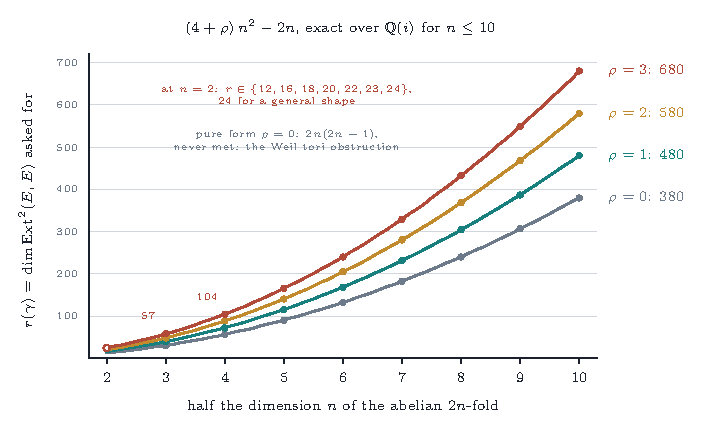
\includegraphics[width=0.86\textwidth]{fig_hankel}
\caption{The dimension $r(\gamma)=(4+\rho)n^{2}-2n$ that
$\Ext^{2}(E,E)$ must have for a complex with Chern character
$\gamma=N\omega_{1}+\sum_{k}c_{k}\theta^{k}$ to meet the polarised criterion,
for the four Hankel ranks $\rho$ of \Cref{thm:p2primenumber}; the dots mark
the values at $n=2,\dots,10$, and at $n=10$ the space $HT^{2}$ has dimension
$780$. The pure form, $\rho=0$, is the bottom curve
$2n(2n-1)$, which no complex attains (\Cref{thm:p2false}); a general shape
lies on the top curve $7n^{2}-2n$. At $n=2$ the weight argument fails for one
pair of weights and seven values occur.}
\label{fig:hankel}
\end{figure}

\begin{proposition}[The Hochschild profile of a polarised character]
\label{prop:p2primeprofile}
In \Cref{setup:p2prime}, let $\rho_{k}$ be the rank of contraction
$HT^{k}(A)\to H^{*}(A,\CC)$ into $\gamma$, put $C_{l}=l!\,c_{l}$, let
$r'$ be the rank of the $(n+1)\times(n+1)$ Hankel matrix $H'=[C_{p+q}]$, and
$d=\dim\ker\bigl((K'H')^{2}-|u|^{2}\bigr)$ with
$K'=\mathrm{antidiag}\bigl((-1)^{a}\binom{n}{a}\bigr)$.
\begin{enumerate}[label=\textup{(\roman*)},leftmargin=2.6em,itemsep=2pt]
\item $\rho_{0}=\rho_{2n}=1$, $\rho_{k}=0$ for $k>2n$, and for
  $1\le k\le2n-1$, $k\ne n$,
  \[
    \rho_{k}=2\binom{2n}{k}+M_{k}\min(k+1,\,2n+1-k,\,r'),\qquad
    M_{k}=\sum_{\substack{i+j=k\\1\le i,j\le n-1}}\binom{n}{i}\binom{n}{j};
  \]
  in the middle degree the same formula holds with $d$ subtracted. In particular $\rho_{k}=\rho_{2n-k}$, and the general
  profiles are $(1,8,24,8,1)$ at $n=2$ and $(1,12,57,112,57,12,1)$ at
  $n=3$.
\item $\chi(E,E)=V\,Q(c)+W$ for a perfect complex with $\ch(E)=\gamma$, where
  $V=\int_{A}\theta^{2n}>0$, $W=(-1)^{n}\int_{A}\omega^{2}>0$ and
  $Q(c)=\sum_{k}(-1)^{k}c_{k}c_{2n-k}$; and $\chi(E,E)$ is even.
\item Granting the compatibility of \Cref{cor:hhfactor}(iii) in every degree,
  $\dim\Ext^{k}(E,E)\ge\rho_{k}$. At $n=2$, at the points with $d=1$ one has
  $\rho_{2}=23$, which is odd, so $\dim\Ext^{2}(E,E)=r(\gamma)$ cannot hold
  there, since $\chi(E,E)$ is even and Serre duality gives
  $\chi(E,E)\equiv\dim\Ext^{2}(E,E)\bmod2$.
\end{enumerate}
\end{proposition}

\begin{proof}
(i) Split $HT^{1}=Q\oplus P$ as in \Cref{thm:hhsplitting}, so that
$HT^{k}=\bigoplus_{i+j=k}\bigwedge^{i}Q\otimes\bigwedge^{j}P$ and $Q$, $P$ act
on the two tensor factors of $H^{*}(A)=H_{+}\otimes H_{-}$ separately. A mixed
monomial kills $\omega$, and on $p(\theta)$ the block of mixed monomials with
fixed index sets $I$, $J$ has entries $C_{s+t+m+m'}$ depending only on
$s+t$ and $m+m'$, so its rank is that of a catalecticant of the binary form
$\sum_{k}c_{k}x^{k}y^{2n-k}/(2n-k)!$, which is $\min(k+1,2n+1-k,r')$ by the
classical Hilbert function of an apolar ideal. The pure sources
$\bigwedge^{k}Q$ and $\bigwedge^{k}P$ kill $\alpha_{-}$ and $\alpha_{+}$
respectively and contract the other class injectively
(\Cref{thm:hhsplitting}(iii)). To see where their images go, use the torus of
the proof of \Cref{thm:p2primenumber}(i) and put $I_{Q}=\{j<n\}$,
$I_{P}=\{j\ge n\}$. The basis vectors $w(f_{j}),c(e_{j})$ of $Q$ have weight
$-\epsilon_{j}$ for $j\in I_{Q}$, the vectors $w(e_{j}),c(f_{j})$ of $P$ have
weight $\epsilon_{j}$ for $j\in I_{P}$, $\theta$ has weight $0$ and
$\alpha_{\pm}$ has weight $\pm\sum_{j}\epsilon_{j}$. If $\xi\in\bigwedge^{k}Q$
is a monomial, $k<2n$, and another monomial $\eta$ of $HT^{k}$ sends
$p(\theta)$ or $\alpha_{-}$ to the weight of $\xi\lrcorner\alpha_{+}$, which is
$+1$ at every $j\in I_{P}$, then it is not $\alpha_{-}$, which would need two
factors from $P$ at every $j\in I_{P}$; so $\eta$ has one factor from $P$ for
each $j\in I_{P}$, $\xi$ has weight at most $-1$ at every $j\in I_{Q}$, and
$k\ge n$. For $k=n$ this forces $\xi$ and $\eta$ to lie in the spans
$D_{Q}\subset\bigwedge^{n}Q$ and $D_{P}\subset\bigwedge^{n}P$ of the $2^{n}$
monomials with one factor for each index. The same holds with $P$ and $Q$
exchanged. A mixed monomial kills
$\omega$, so for $k<n$ the matrix of contraction is block triangular, the pure
blocks injective onto targets of their own, and $\rho_{k}$ is $2\binom{2n}{k}$
plus the rank of the mixed blocks; for $k>n$ the formula follows from
\Cref{lem:rankduality}, which also gives $\rho_{k}=\rho_{2n-k}$.

For $k=n$, a pure monomial outside $D_{Q}\cup D_{P}$ repeats an index, so it
kills $1$ and $t_{j}$ at that index and hence $p(\theta)$, and keeps a target
of its own; no mixed monomial reaches the weights $\sum_{j\in I_{P}}
\epsilon_{j}$ and $-\sum_{j\in I_{Q}}\epsilon_{j}$ of the images of
$D_{Q}\oplus D_{P}$, since it would need $n$ factors from one side. So
$\rho_{n}$ is the value of the formula minus the dimension of the kernel of the
block $\beta\colon D_{Q}\oplus D_{P}\to T_{1}\oplus T_{2}$, $T_{1}$ and $T_{2}$
being the targets of those two weights. For $R\subseteq I_{Q}$ and
$J\subseteq I_{P}$ let $X_{R}=\prod_{j\in I_{Q}}z_{j}$ with $z_{j}=w(f_{j})$ for
$j\in R$ and $c(e_{j})$ otherwise, and $Y_{J}=\prod_{j\in I_{P}}z_{j}$ with
$z_{j}=c(f_{j})$ for $j\in J$ and $w(e_{j})$ otherwise, the factor of largest
index acting first, and write $\alpha_{+}=a\,e_{0}\cdots e_{2n-1}$,
$\alpha_{-}=b\,f_{0}\cdots f_{2n-1}$. Since
$\theta^{2n}/(2n)!=\prod_{j}t_{j}=\prod_{j}s_{j}\,e_{0}\cdots e_{2n-1}
f_{0}\cdots f_{2n-1}$, the normalisation of \Cref{setup:p2prime} gives
$ab=(-1)^{n}\prod_{j}s_{j}$. As the $t_{j}$ are even with $t_{j}^{2}=0$,
$p(\theta)=\sum_{S}\mu_{|S|}\prod_{j\in S}t_{j}$. Each operator acts on one
factor of $H^{*}(A)=\bigotimes_{j}\bigwedge^{*}\langle e_{j},f_{j}\rangle$
with the Koszul sign of the factors before it, and in each of the four
products below the parities of those factors do not depend on $R$ or $J$;
the signs are $+1$ on $p(\theta)$, $\epsilon_{1}=(-1)^{n(n-1)/2}$ for $X_{R}$ on
$\alpha_{+}$ and $\epsilon_{2}=(-1)^{n(3n-1)/2}$ for $Y_{J}$ on $\alpha_{-}$.
With $\tau_{R}=e_{n}\cdots e_{2n-1}\prod_{j\in R}t_{j}$ and
$\tau'_{R'}=f_{0}\cdots f_{n-1}\prod_{j\in R'}t_{j}$, and using
$c(f_{j})t_{j}=-is_{j}e_{j}$, $c(e_{j})t_{j}=is_{j}f_{j}$ and
$e_{j}f_{j}=-is_{j}t_{j}$, one finds
\begin{align*}
  X_{R}\lrcorner\,\alpha_{+}&=\epsilon_{1}a\prod_{j\in R}(is_{j})\,\tau_{R},&
  Y_{J}\lrcorner\,p(\theta)&=\sum_{R}\mu_{|J|+|R|}\prod_{j\in J}(-is_{j})\,\tau_{R},\\
  Y_{J}\lrcorner\,\alpha_{-}&=\epsilon_{2}b\prod_{j\in I_{P}\setminus J}(-is_{j})\,
    \tau'_{I_{P}\setminus J},&
  X_{R}\lrcorner\,p(\theta)&=\sum_{R'}\mu_{n-|R|+|R'|}\prod_{j\in I_{Q}\setminus R}
    (is_{j})\,\tau'_{R'}.
\end{align*}
For $x=\sum_{R}x_{R}X_{R}$ and $y=\sum_{J}y_{J}Y_{J}$ put
$\tilde x_{R}=\prod_{j\in R}(is_{j})\,x_{R}$ and
$\tilde y_{J}=\prod_{j\in J}(-is_{j})\,y_{J}$, and let
$\Pi_{P}=\prod_{j\in I_{P}}(-is_{j})$, $\Pi_{Q}=\prod_{j\in I_{Q}}(is_{j})$.
Then $\beta(x,y)=0$ says
\[
  \epsilon_{1}a\,u\,\tilde x_{R}=-\sum_{J}\mu_{|J|+|R|}\,\tilde y_{J},
  \qquad
  \epsilon_{2}b\,\bbar u\,\Pi_{P}(-1)^{|J|}\tilde y_{J}
  =-\Pi_{Q}\sum_{R}\mu_{2n-|R|-|J|}(-1)^{|R|}\tilde x_{R}
\]
for all $R$ and $J$. So $\tilde x_{R}=g_{|R|}$ and $(-1)^{|J|}\tilde y_{J}=h_{|J|}$
depend only on $|R|$ and $|J|$, and with $D=\operatorname{diag}\bigl((-1)^{c}
\binom{n}{c}\bigr)$ and the exchange matrix $J_{0}$, so that $DJ_{0}=K'$ and
$J_{0}DJ_{0}=(-1)^{n}D$, the conditions read
$\epsilon_{1}a\,u\,g=-H'Dh$ and $\epsilon_{2}b\,\bbar u\,\Pi_{P}h=-\Pi_{Q}
J_{0}H'J_{0}Dg$. Eliminating $h$ gives $(H'K')^{2}g=\lambda g$ with
$\lambda=(-1)^{n}\epsilon_{1}\epsilon_{2}\,ab\,|u|^{2}\,\Pi_{P}/\Pi_{Q}$, and
$\epsilon_{1}\epsilon_{2}=(-1)^{n}$, $ab=(-1)^{n}\prod_{j}s_{j}$,
$\Pi_{P}/\Pi_{Q}=(-1)^{n}\prod_{j}s_{j}$, so $\lambda=|u|^{2}$. Conversely an
eigenvector $g$ determines $h$, $x$ and $y$. Hence $\dim\ker\beta=
\dim\ker\bigl((H'K')^{2}-|u|^{2}\bigr)=d$, as $H'K'$ and $K'H'$ are
conjugate.

(ii) $\ch(E)^{\vee}$ changes the sign of
the components of odd codegree, $\omega\theta=0$ kills the cross terms, and
Hodge--Riemann gives $W>0$; parity holds because the Chern character of a
perfect complex on a complex torus is integral, and the intersection form on
$\bigwedge^{2n}H^{1}(A,\ZZ)$ pairs each monomial only with its complement, so
$\int x^{2}$ is even. (iii) is the argument of \Cref{cor:hhfactor}(iii).
\end{proof}

The profile also shows what the polarised criterion leaves unconstrained. For
the pure form, \Cref{thm:p2endo}(iv) derives $\dim\End(E)\ge3$ at $n=2$ and
$n=3$ from $\chi(E,E)>0$. For a polarised character, $\chi(E,E)=VQ(c)+W$ can
have either sign, and when it is small enough the Euler characteristic forces
nothing. At $n=2$, in the model of \Cref{setup:model} with $d=1$, where
$\int\eta^{4}=24$ and $\int\omega_{1}^{2}=8$ (see the proof of
\Cref{prop:p2primelocus}), the character $\omega_{1}+p(\eta)$ with
$c=(2,1,0,1,-1)$ has $Q(c)=2c_{0}c_{4}-2c_{1}c_{3}+c_{2}^{2}=-6$, so
$\chi(E,E)=-144+8=-136$, and a simple object is not excluded.

\begin{proposition}[The Hodge locus of a polarised character]
\label{prop:p2primelocus}
\begin{enumerate}[label=\textup{(\roman*)},leftmargin=2.6em,itemsep=2pt]
\item Let $T$ be a complex torus, let $x$ be a real class of type $(k,k)$ on
  $T$, and for $v\in\Hom(H^{1,0},H^{0,1})=H^{1}(T_{T})$ let $J_{v}$ be the
  complex structure on the underlying real torus with $H^{1,0}_{v}=(1+v)H^{1,0}$.
  Then $x$ is of type $(k,k)$ for $J_{v}$ if and only if $v\lrcorner x=0$. So
  in this chart the Hodge locus of $x$ is the linear space
  $\Ann_{H^{1}(T_{T})}(x)$, and it coincides with its first-order locus.
\item Let $J$ be any complex structure on the real torus underlying $A$. If
  $\theta^{k}$ is of type $(k,k)$ for $J$ for some $1\le k\le2n-1$, then
  $\theta$ is of type $(1,1)$ for $J$.
\item In \Cref{setup:p2prime} with $n\ge3$, the germ at $A$ of the Hodge locus
  of $\gamma$ among all complex structures is the polarised Weil family
  $\cD_{n,n}$, of dimension $n^{2}$, if $c_{k}\ne0$ for some $1\le k\le2n-1$,
  and the family of all $K$-linear deformations, of dimension $2n^{2}$,
  otherwise. In the first case the connected component of the Hodge locus
  through $A$ is $\cD_{n,n}$, and all its members are abelian varieties
  polarised by $\theta$.
\item For $n=2$ the same holds, with one exception: if $c_{1}=c_{3}=0$ and
  $c_{2}^{2}\int_{A}\theta^{4}=\tfrac34\int_{A}\omega^{2}$, the germ has
  dimension $5$. In the model of \Cref{setup:model} this is
  the character $N\omega_{1}\pm\tfrac{d}{2}N\eta^{2}+c_{0}+c_{4}\eta^{4}$;
  with rational data the ratio is attained exactly in the families of trivial
  discriminant.
\end{enumerate}
\end{proposition}

\begin{proof}
(i) Write $D_{v}$ for the derivation of $\bigwedge^{*}H^{1}$ extending $v$.
Since $v^{2}=0$ on $H^{1}$, $\bigwedge^{*}(1+v)=\exp(D_{v})$, so the Hodge
filtration of $J_{v}$ is $F^{p}_{v}=\exp(D_{v})F^{p}$. Now
$\exp(-D_{v})x=\sum_{m}(-1)^{m}D_{v}^{m}x/m!$ with $D_{v}^{m}x$ of type
$(k-m,k+m)$, so $x\in F^{k}_{v}$ exactly when $D_{v}x=v\lrcorner x=0$; and a
real class lies in $F^{k}_{v}\cap\overline{F^{k}_{v}}=H^{k,k}_{v}$ as soon as
it lies in $F^{k}_{v}$. (ii) Let $t\mapsto t_{J}$ be the circle acting on
$H^{p,q}$ by $t^{p-q}$. It acts on $\bigwedge^{*}H^{1}(A,\RR)$ by algebra
automorphisms and fixes $\theta^{k}$, so the path $t\mapsto t_{J}\theta$ lies in
$\{y\in\bigwedge^{2}H^{1}(A,\RR):y^{k}=\theta^{k}\}$. At a nondegenerate $y$
the differential $h\mapsto k\,y^{k-1}h$ of $y\mapsto y^{k}$ is injective on
$\bigwedge^{2}$ when $2+(k-1)\le2n$, by the linear hard Lefschetz theorem for
the symplectic form $y$ on a space of dimension $4n$: for a nondegenerate
$y\in\bigwedge^{2}U^{\vee}$ on a real space $U$ of dimension $2m$,
multiplication by $y^{j}$ is injective from $\bigwedge^{p}$ to
$\bigwedge^{p+2j}$ whenever $p+j\le m$, because $y$ generates an
$\mathfrak{sl}_{2}$-action on $\bigwedge^{*}U^{\vee}$ in which $\bigwedge^{p}$
has weight $p-m$; here $m=2n$, $p=2$ and $j=k-1$. So near $\theta$ that set
is discrete, the path is constant, and $\theta$ is of type $(1,1)$. The bound
$k\le2n-1$ is sharp, since $\theta^{2n}$ is a multiple of the volume form for
every complex structure. (iii) By
(i), applied to each homogeneous component, the Hodge locus of $\gamma$ in the
chart is $\Ann_{H^{1}(T_{A})}(\gamma)$, the part of $\Ann_{HT^{2}}(\gamma)$ in
$H^{1}(T_{A})$. In the description of \Cref{thm:p2primenumber}(i) that part is
$x=w=0$ with $(0,\lambda,0)\in\ker H$; the vector $(0,1,0)$ lies in $\ker H$
exactly when $\mu_{1}=\dots=\mu_{2n-1}=0$, so the part is spanned by the $n^{2}$
vectors $v^{1}_{ab}+v^{2}_{ab}$, which span $T_{[A]}\cD_{n,n}$, when some
$c_{k}$ with $1\le k\le2n-1$ is nonzero, and by all $v^{1}_{ab},v^{2}_{ab}$,
the $K$-linear deformations, otherwise. A germ of submanifold of dimension
$n^{2}$ inside a linear space of the same dimension is that space. On
$\cD_{n,n}$ the class $\theta$ stays of type $(1,1)$ and nondegenerate, so the
signature of the hermitian form it defines is constant and every member is
polarised by $\theta$. The same argument at every member shows that
$\cD_{n,n}$ is open in the Hodge locus; it is closed in the space of complex
structures, since $K$-linearity is a closed condition and a limit of positive
hermitian forms that stays nondegenerate stays positive; and it is
connected. (iv) At $n=2$ the weight argument of
\Cref{thm:p2primenumber}(i) fails for one pair of weights. The other weights
contribute as in (iii): the $K$-linear deformations, of dimension $8$, when
$c_{1}=c_{2}=c_{3}=0$, and the tangent space of the polarised family, of
dimension $4$, otherwise. The remaining pair of weights couples
$\xi'\in\Hom(V_{+}^{1,0},V_{-}^{0,1})$ with
$\xi''\in\Hom(V_{-}^{1,0},V_{+}^{0,1})$. Choose bases $x_{\pm,k}$ of
$V_{\pm}^{1,0}$ and $y_{\pm,k}$ of $V_{\pm}^{0,1}$, $k=1,2$, with
$\theta=\sum_{k}(x_{+,k}y_{-,k}+x_{-,k}y_{+,k})$, put
$\beta_{\pm}=x_{\pm,1}x_{\pm,2}y_{\pm,1}y_{\pm,2}$, a generator of
$\bigwedge^{4}V_{\pm}$, and write $\omega=u_{+}\beta_{+}+u_{-}\beta_{-}$. The component of
$(\xi'+\xi'')\lrcorner\gamma$ of degree $3$ in $V_{-}$ and $1$ in $V_{+}$ is
$u_{-}\,\xi''\lrcorner\beta_{-}+c_{2}\,\xi'\lrcorner\theta^{2}$, because
$c_{1}=c_{3}=0$ and $\xi'\lrcorner\theta^{4}=4\theta^{3}(\xi'\lrcorner\theta)=0$;
the component of degree $3$ in $V_{+}$ is the same with $+$ and $-$
exchanged.
Here $\xi'\lrcorner\theta$ lies in the line spanned by $y_{-,1}y_{-,2}$, so
$\xi'\lrcorner\theta^{2}=2\theta\,(\xi'\lrcorner\theta)$ is a multiple of
$\theta\,y_{-,1}y_{-,2}$. The map $\xi''\mapsto\xi''\lrcorner\beta_{-}$ is
injective, and $\theta\,y_{-,1}y_{-,2}=\xi''_{0}\lrcorner\beta_{-}$ for
$\xi''_{0}(x_{-,1})=-y_{+,2}$, $\xi''_{0}(x_{-,2})=y_{+,1}$, which has
$\xi''_{0}\lrcorner\theta=2y_{+,1}y_{+,2}$. With $\xi'_{0}$ defined in the
same way, a solution has $\xi'=a\xi'_{0}$ and $\xi''=b\xi''_{0}$ with
$u_{+}a+4c_{2}b=0$ and $4c_{2}a+u_{-}b=0$. So the annihilator meets this
pair in a line when $16c_{2}^{2}=u_{+}u_{-}$ and in zero otherwise; since
$\theta^{4}=24\,\beta_{+}\beta_{-}$ and
$\omega^{2}=2u_{+}u_{-}\,\beta_{+}\beta_{-}$, the condition is
$c_{2}^{2}\int\theta^{4}=\frac34\int\omega^{2}$.
In the model, where $\int\theta^{4}$ and $\int\omega^{2}$ are $24$ and
$2|u|^{2}$ times the same volume, the ratio reads $|u|=4|c_{2}|$. In the
model of \Cref{setup:model}, $\eta^{4}=4!\prod_{j}\epsilon_{j}x_{j}y_{j}$
gives $\int\eta^{4}=24$; in $\omega_{1}^{2}$ only the products
$w^{(T)}w^{(T^{c})}$ survive, and each of the eight with $|T|$ even contributes
$d^{2}$, so $\int\omega_{1}^{2}=8d^{2}$; likewise $\int\omega_{2}^{2}=8d$, and
$\omega_{1}\omega_{2}=0$ because $T$ and $T^{c}$ have the same parity. This
gives $c_{2}=\pm dN/2$. For a general rational
Weil class $\omega=x\omega_{1}+y\omega_{2}$ and hermitian form
$\mathrm{diag}(-a_{1},-a_{2},a_{3},a_{4})$ one has
$\int\omega^{2}=8d\,\Nm_{K/\QQ}(y+x\sqrt{-d})$ and
$\int\theta^{4}=24\,a_{1}a_{2}a_{3}a_{4}$, so the ratio asks
$(c_{2}/N)^{2}=d\,\Nm_{K/\QQ}(y+x\sqrt{-d})/(4a_{1}a_{2}a_{3}a_{4})$, a rational
square exactly when $a_{1}a_{2}a_{3}a_{4}$ is a norm from $K$.
\end{proof}

The argument of \Cref{thm:p2false} therefore does not extend to the
polarised form. A semiregular complex deforms along the Hodge locus of its
Chern character. For the pure form that locus is the whole
$2n^{2}$-dimensional family of $K$-linear tori, whose very general member is
not algebraic; for a polarised character with some $c_{k}\ne0$,
$1\le k\le2n-1$, it is the polarised family itself, all of whose members are
abelian varieties, and the argument through Weil tori has nothing to act on.
This concerns the argument run on $E$ itself: an autoequivalence can still
remove a component, and a line bundle twist is how the argument reaches the
polarised characters of \Cref{thm:p2primenumber}(v). The only other case it
can reach is the exceptional ratio of (iv), where the Hodge locus leaves the
polarised family.

\begin{remark}[The exceptional ratio at $n=2$]\label{rem:p2primeexceptional}
At $n=2$, with $c_{1}=c_{3}=0$ and $c_{2}^{2}\int\theta^{4}=\frac34\int\omega^{2}$,
put $\gamma_{2}=\omega+c_{2}\theta^{2}$, and let $\mathfrak{g}$ be its
stabiliser in $\mathfrak{gl}(H^{1}(A,\RR))$. In the notation of the proof of
\Cref{prop:p2primelocus}(iv), put $(e_{1},\dots,e_{4})=(x_{+,1},x_{+,2},
y_{+,1},y_{+,2})$ and $(f_{1},\dots,f_{4})=(y_{-,1},y_{-,2},-x_{-,1},
-x_{-,2})$; then $\theta=\sum_{j}e_{j}f_{j}$,
$\omega=u_{+}e_{1234}+u_{-}f_{1234}$ with $e_{1234}=e_{1}\wedge\dots\wedge
e_{4}$, and the ratio is $16c_{2}^{2}=u_{+}u_{-}$. Passing to the basis
$se_{j}$, $s^{-1}f_{j}$ with $s^{8}=u_{+}/u_{-}$ fixes $\theta$ and makes the
two coefficients of $\omega$ equal, and passing from $f_{j}$ to
$\sqrt{-1}f_{j}$, if necessary, changes the sign of $\theta^{2}$ and fixes
$f_{1234}$. So over
$\CC$ the class $\gamma_{2}$ is a nonzero multiple of
\[
  \tfrac12\bigl(e_{1234}+f_{1234}\bigr)-\tfrac18\Bigl(\textstyle\sum_{j}e_{j}f_{j}\Bigr)^{2},
\]
which is the Cayley form $\frac12\omega_{0}^{2}+\Re\Omega_{0}$ of $\CC^{4}$,
with $\omega_{0}=\frac{\sqrt{-1}}{2}\sum dz_{j}\wedge d\bbar z_{j}$ and
$\Omega_{0}=dz_{1}\wedge\dots\wedge dz_{4}$, written in the basis
$e_{j}=dz_{j}$, $f_{j}=d\bbar z_{j}$ \cite{HL82}. The stabiliser
of the Cayley form in $\GL(8,\RR)$ is $\mathrm{Spin}(7)$, acting on $\RR^{8}$
by its spin representation, and its invariants in $\bigwedge^{*}\RR^{8}$ are
spanned by $1$, the form and the volume form \cite{Bry87}. A stabiliser in
$\mathfrak{gl}$ is cut out by linear equations, so it commutes with
extension of scalars, and $\mathfrak{g}\otimes\CC\cong\mathfrak{so}(7,\CC)$
acts on $H^{1}(A,\CC)$ by the spin representation, irreducibly, with
invariants in $\bigwedge^{*}H^{1}$ spanned by $1$, $\gamma_{2}$ and the
class of a point. At an ordinary ratio the stabiliser is the Lie algebra
$\mathfrak{su}(2,2)$ of the Hodge group, of dimension $15$, which also fixes
$\gamma_{2}$ here.

The real form is $\mathfrak{so}(4,3)$. The spin representation of
$\mathfrak{so}(7,\CC)$ carries an invariant symmetric form, unique up to a
scalar by irreducibility, so $\mathfrak{g}$ preserves a real symmetric form
$B$ on $H^{1}(A,\RR)$. On $H^{1}(A,\CC)=V_{+}\oplus V_{-}$ the subalgebra
$\mathfrak{su}(2,2)\otimes\CC=\mathfrak{sl}(V_{+})$ acts on $V_{+}$ and
dually on $V_{-}$, and its only invariant bilinear forms pair $V_{+}$ with
$V_{-}$; so $B$ is a multiple of the real part of the hermitian form of
$\theta$, of signature $(4,4)$, and $\mathfrak{g}\subseteq\mathfrak{so}(4,4)$.
The real forms of $\mathfrak{so}(7,\CC)$ are the $\mathfrak{so}(p,q)$ with
$p+q=7$, and the maximal compact subalgebra $\mathfrak{so}(p)\oplus
\mathfrak{so}(q)$ lies in a maximal compact subalgebra of
$\mathfrak{so}(4,4)$, which is $\mathfrak{so}(4)\oplus\mathfrak{so}(4)\cong
\mathfrak{su}(2)^{4}$. A simple subalgebra of $\mathfrak{su}(2)^{4}$ projects
injectively to a factor, so it has dimension $3$; hence $p,q\le4$, and
$\{p,q\}=\{4,3\}$. So $\gamma_{2}$ is the invariant $4$-form of
$\mathrm{Spin}(4,3)$, a split form of the Cayley form.

The Hodge decomposition of $\mathfrak{g}$ has dimensions $5$, $11$, $5$.
Indeed, the complex structure $J$ of $A$ fixes the class $\gamma_{2}$ of type
$(2,2)$ and lies in the image of the Hodge group, which is connected and
contained in the group of $\mathfrak{g}$; as $J^{2}=-1$ is the nontrivial
central element of $\mathrm{Spin}(4,3)$, the image of $J$ in
$\mathrm{SO}(7,\CC)$ is an involution with $2k$ eigenvalues $-1$ and $k$
odd, since a lift of such an involution squares to $(-1)^{k}$. The
eigenvalue $-1$ of $\operatorname{Ad}J$ on $\mathfrak{g}\otimes\CC$ then has
multiplicity $2k(7-2k)$, which is $10$ or $6$, and it contains the
$(-1)$-eigenspace of $\mathfrak{sl}(V_{+})$, of dimension $8$; so $k=1$, and
$\mathfrak{g}^{-1,1}\oplus\mathfrak{g}^{1,-1}$ has dimension $10$.

The Hodge locus of $\gamma$ near $A$ is the orbit of $A$ under the connected
real group $G$ of $\mathfrak{g}$, since that orbit has dimension
$\dim\mathfrak{g}^{-1,1}=5$ and lies in the locus, which near $A$ is smooth of
dimension $5$ (\Cref{prop:p2primelocus}(i) and (iv)). The Hodge group of a
very general member $T$ has Lie algebra an ideal of $\mathfrak{g}$, hence all
of it, so the Hodge classes of $T$ are $1$, $\gamma_{2}$ and the class of a
point, and $\NS(T)=0$. The locus therefore contains tori that are not
algebraic, and the proof of \Cref{thm:p2false} can be started there. It
breaks down at its last step: \Cref{prop:weiltorussheaves} needs a K\"ahler
class on which the degree-four Chern character integrates to zero, and here
\[
  \int_{A}\gamma_{2}\,\kappa_{h}^{2}
  =\frac{|c_{2}|}{6}\Bigl(\operatorname{sign}(c_{2})\,\sigma_{2}(h)
    +4\operatorname{Re}\bigl(\phi\det h_{01,23}\bigr)\Bigr)\int_{A}\theta^{4},
  \qquad|\phi|=1,
\]
for the K\"ahler class $\kappa_{h}=i\sum h_{jk}z_{j}\wedge\bbar z_{k}$ of a
positive hermitian $h$ in a unitary frame for $\theta$, and the right-hand
side has the sign of $c_{2}$. Indeed, writing
$h=\sum_{j}\lambda_{j}w_{j}w_{j}^{*}$ with $(w_{j})$ orthonormal,
Cauchy--Binet gives
$\sigma_{2}(h)\pm4\operatorname{Re}(\phi\det h_{01,23})
=\sum_{j<k}\lambda_{j}\lambda_{k}\bigl(1\pm4\operatorname{Re}(\phi\,\xi_{01}\bbar\xi_{23})\bigr)$
with $\xi=w_{j}\wedge w_{k}$ of norm one. The Pl\"ucker relation and the
inequality of the means give $|\xi_{01}\xi_{23}|\le\frac14$, so each term is
nonnegative, and by Parseval the brackets sum to $6$ over $j<k$, so the sum is
at least $6\min_{j}\lambda_{j}^{2}>0$. Since $G$ fixes $\gamma_{2}$ and carries
K\"ahler cones to K\"ahler cones, the same holds on every member of the locus.
So at this ratio the argument excludes at most a torsion-free sheaf with
$c_{2}>0$, which Bogomolov's inequality already forbids to be
$\theta$-semistable, and it excludes no complex. With
$R=c_{2}^{2}\int\theta^{4}\big/\!\int\omega^{2}$, the ratio that equals
$\frac34$ here, \Cref{fig:kahlersign} draws the infimum of the ratio as a
function of $R$. Since Markman's theorem settles every Weil
fourfold, this remark concerns the shape of \textup{(P2$'$)}, not the
conjecture.
\end{remark}

\begin{figure}[tbp]
\centering
  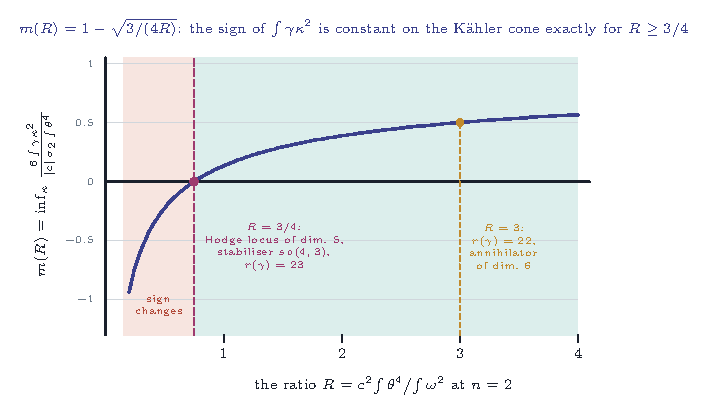
\includegraphics[width=0.86\textwidth]{fig_kahlersign}
\caption{The exceptional ratio of \Cref{rem:p2primeexceptional}. By the
identity displayed there, which is linear in $\gamma$, the infimum over the
K\"ahler cone of $6\int\gamma\kappa^{2}\big/\bigl(|c|\,\sigma_{2}(h)\int
\theta^{4}\bigr)$ is $m(R)=1-\sqrt{3/(4R)}$, approached at the boundary of the
cone by a positive hermitian form of rank two whose Pl\"ucker coordinates
satisfy $|\xi_{01}\xi_{23}|=\frac14$. It is negative exactly for $R<3/4$, and
$R=3/4$ is also where the Hodge locus of $\gamma$ jumps from dimension $4$ to
$5$ and its stabiliser becomes $\mathfrak{so}(4,3)$.}
\label{fig:kahlersign}
\end{figure}

\begin{remark}[The obstructions for a polarised character]
\label{rem:p2primesurvive}
The obstruction theorems proved from \Cref{sec:semireg} on for a Chern
character on the Weil line divide as follows for a polarised character. The
following hold unchanged, with
$r(\gamma)$ in place of $2n(2n-1)$ where a number occurs:
\Cref{thm:linebundle} and \Cref{cor:noline}, whose only hypothesis is that
$\ch(E)$ stay of Hodge type to first order along $\cD_{n,n}$;
\Cref{thm:positivity} and \Cref{cor:nofiltered}, since a polarised character
is a flat Hodge class in every degree; \Cref{lem:finiteproduct}; and the
first two parts of \Cref{thm:p2numerical}, which become
\Cref{thm:p2primenumber}(iv). The following hold only when
$c_{0}=\dots=c_{2n-2}=0$, so that $H^{0,2}$ still kills $\gamma$:
\Cref{thm:rankzero}, \Cref{prop:concentrated}, \Cref{cor:kernelfamily},
\Cref{thm:weakfails} and \Cref{thm:p2forces}(iii). The following hold only
when $\ker H$ contains a vector with $w\ne0$, which needs $\rho\le2$, the
vector giving a compensated class of $P\wedge Q$ with a component in
$T_{+}\otimes T_{-}$: \Cref{thm:p2forces}(iv), \Cref{cor:p2shape} and
\Cref{thm:p2support}. The following do not extend: \Cref{thm:p2false},
outside \Cref{thm:p2primenumber}(v); the positivity of $\chi(E,E)$ in
\Cref{prop:objectsize} and with it \Cref{thm:p2endo}(i)--(iii), by
\Cref{prop:p2primeprofile}(ii); and \Cref{thm:nosum}. So for a general shape,
$\rho=3$, what these results exclude is a line bundle summand off the
polarisation line and a Chern character effective in the exponential basis,
and nothing else; \Cref{prop:scalaratiyah} below extends the first to
summands with a scalar Atiyah class. An object with no such summand, whose
Chern character is not effective, and with $\dim\Ext^{2}(E,E)=7n^{2}-2n$, is
not excluded by anything proved here, and none is known; by
\Cref{lem:p2primesummands} below it may be taken indecomposable.
\end{remark}

\begin{proposition}[Summands with a scalar Atiyah class]\label{prop:scalaratiyah}
Let $A$ be of $(K,-1,n)$-Weil type with $n\ge2$, let $T=T_{[A]}\cD_{n,n}$, and
let $E$ be a perfect complex on $A$ with $v\lrcorner\ch(E)=0$ for every
$v\in T$. Suppose $E$ has a direct summand $F[p]$ with
$\mathrm{At}(F)=\delta\cdot\id_{F}$, where $\delta$ is a real class of type
$(1,1)$ that is not a real multiple of $\theta$, and $\rk F\ne0$. Then there is
$v\in T$ with $\operatorname{ev}_{E}(v)\ne0$ and
$\sigma_{E}(\operatorname{ev}_{E}(v))=0$. In particular no finite direct sum
of shifted bundles $\pi_{*}L$, $\pi$ an isogeny, among them the simple
semi-homogeneous bundles, has a polarised character $\gamma$ with $N\ne0$ and
injective semiregularity map.
\end{proposition}

\begin{proof}
As in \Cref{thm:linebundle}, $\operatorname{ev}_{E}(v)=v\lrcorner\mathrm{At}(E)$
on $H^{1}(T_{A})$ and the Atiyah class of a direct sum is block diagonal, so
the component of $\operatorname{ev}_{E}(v)$ in $\Ext^{2}(F,F)$ is
$(v\lrcorner\delta)\cdot\id_{F}$; the map $z\mapsto z\cdot\id_{F}$ on
$H^{0,2}$ is injective because $\mathrm{tr}(z\cdot\id_{F})=\rk(F)\,z$, and
some $v\in T$ has $v\lrcorner\delta\ne0$ by \Cref{prop:rigidity}(i). On the
other hand $\sigma_{E}(\operatorname{ev}_{E}(v))=v\lrcorner\ch(E)=0$. For the
last sentence, the proof of \Cref{lem:blocks}(i) gives
$\mathrm{At}(\pi_{*}L)=\delta\cdot\id$ with $\pi^{*}\delta=c_{1}(L)$ for any
line bundle $L$, and $\ch(\pi_{*}L)=\rk(\pi_{*}L)\,e^{\delta}$; if every
$\delta$ were a multiple of $\theta$ the Chern character of the sum would lie
in $\QQ[\theta]$, which does not contain $\omega$ because $\omega\theta=0$ and
$\theta^{n+1}\ne0$.
\end{proof}

\Cref{thm:semiregclosure} asks that $\sigma_{E}$ be injective, but its proof
uses only that the relative deformations of $E$ dominate the family, and
Pridham's form of \Cref{thm:BF}, in which $\sigma_{E}$ annihilates every
obstruction, gives this under a weaker hypothesis. That hypothesis allows an
object that is obstructed to first order, which is exactly the way in which
\Cref{thm:linebundle}, \Cref{cor:noline} and \Cref{prop:scalaratiyah} exclude
an object.

\begin{proposition}[A flatness form of the criterion]\label{prop:p2flat}
Let $n\ge2$, $s_{0}\in\cD_{n,n}$, and let $E$ be a bounded complex of vector
bundles on $A_{s_{0}}$ with $\ch(E)=N\omega_{1}+\sum_{k}c_{k}\theta^{k}$ and
$N\ne0$. Let $K_{E}$ be the base of a miniversal deformation of $E$ on the
fixed variety $A_{s_{0}}$, put $e=\dim\Ext^{1}(E,E)$ and
$k=\dim\ker\sigma_{E}$. By \Cref{thm:BF} in Pridham's form, $\sigma_{E}$
annihilates every obstruction, both on $A_{s_{0}}$ and along the Artinian
deformations of $A_{s_{0}}$ in $\cD_{n,n}$.
\begin{enumerate}[label=\textup{(\roman*)},leftmargin=2.6em,itemsep=2pt]
\item $\dim K_{E}\ge e-k$.
\item If $\dim K_{E}=e-k$, then $\Sigma=\cD_{n,n}$, and the Hodge conjecture
  holds in every degree for every member of the family with
  $\Hg(A)=\SU(V,H)$.
\item $\dim K_{E}=e-k$ as soon as the cone
  $\{\xi\in\Ext^{1}(E,E):\xi\circ\xi=0\}$ has codimension $k$.
\end{enumerate}
For $k=0$ this is \Cref{thm:semiregclosure}.
\end{proposition}

\begin{proof}
Let $R$ be the completed local ring of $\cD_{n,n}$ at $s_{0}$, regular of
dimension $n^{2}$. By hypothesis $\ker\sigma_{E}$ is a complete obstruction
space for the deformations of the pair $(A_{s},E)$ over Artinian $R$-algebras,
whose relative tangent space is $\Ext^{1}(E,E)$; so this functor has a hull
$P/J$ with $P=R[[x_{1},\dots,x_{e}]]$ and $J$ generated by at most $k$
elements \cite{FM98}, and its fibre over the closed point of $R$ is a hull of
the absolute functor, of dimension $\dim K_{E}$. Krull's height theorem gives
$\dim P/J\ge n^{2}+e-k$, and the same count on the fibre gives (i). If
$\dim K_{E}=e-k$, the dimension inequality for a local homomorphism
\cite[Theorem~15.1]{Mat86} gives $\dim P/J\le n^{2}+e-k$, so equality holds, $J$
has height $k$ and is generated by a regular sequence, $P/J$ is
Cohen--Macaulay, and it is flat over $R$ by miracle flatness
\cite[Theorem~23.1]{Mat86}: a local homomorphism from a regular local ring to
a Cohen--Macaulay local ring is flat exactly when the dimension of the target
is the dimension of the source plus that of the fibre, and here both sides
equal $n^{2}+e-k$. The analytic Kuranishi germ of pairs, as in the
proof of \Cref{thm:p2false}, has $P/J$ as its completion, so it is flat over
the germ of $\cD_{n,n}$ at $s_{0}$ and therefore open onto a neighbourhood
$U$ of $s_{0}$. Every $A_{s}$ with $s\in U$ then carries a bounded complex of
vector bundles, algebraic by GAGA, whose Chern character is the parallel
transport of $\ch(E)$, so $N\omega_{1,s}$ differs from an algebraic class by a
polynomial in $\theta$ and is algebraic; \Cref{cor:allornothing} gives (ii).
For (iii), the quadratic part of the Kuranishi map of $E$ is
$\xi\mapsto\xi\circ\xi$, so the tangent cone of $K_{E}$ lies in the cone of the
hypothesis, and $\dim K_{E}\le e-k$. Every step uses only deformations along
$\cD_{n,n}$, which are projective, whereas the proof of \Cref{thm:p2false}
needs non-projective ones.
\end{proof}

No object is known that meets (iii) with $k>0$. Among direct sums the
flatness form fails for a large class (\Cref{rem:flatsums} below); for
indecomposable objects nothing in this paper excludes it, and the proposition
says only that injectivity of $\sigma_{E}$ is more than propagation needs.

\subsection{Candidate objects for the polarised criterion}

The polarised criterion asks for one perfect complex. The results below say
what such a complex can be made of, for $K$ imaginary quadratic: a direct sum
meets the criterion only through one indecomposable summand
(\Cref{lem:p2primesummands}); no sum of objects whose Ext algebra is an
exterior algebra meets it (\Cref{cor:naturalsums}); the Orlov products of
secant objects meet its twisted form, with $\dim\Ext^{2}$ equal to the number
of \Cref{thm:p2primenumber}, at $n=2$ and $n=3$ (\Cref{thm:twistedcert}), and
cannot meet it at $n=4$ when the factors have no negative self-extensions
(\Cref{prop:orlovfour}); line bundles on smooth divisors, which give the
certificates, give no factor from $n=4$ on, nor do bundles restricted from
the abelian variety at $n=5$ (\Cref{prop:divisortemplate}); and at $n=4$ a combination of natural objects needs
at least eight of them, on one conic (\Cref{thm:minimalsupport}). None of
this gives a new case of the Hodge conjecture: the certificates are for
twisted objects, in families where Markman's theorem already holds.

\begin{lemma}[The summands of an object meeting the criterion]
\label{lem:p2primesummands}
Let $A$ be a member of a $(K,-1,n)$-Weil family, $K$ imaginary quadratic and
$n\ge2$, let $T=T_{[A]}\cD_{n,n}\subseteq H^{1}(T_{A})$, and let
$E=\bigoplus_{i}F_{i}[k_{i}]$ be a finite direct sum of perfect complexes with
$v\lrcorner\ch(E)=0$ for every $v\in T$, as holds for every polarised character
$N\omega_{1}+\sum_{k}c_{k}\theta^{k}$. Suppose that $\sigma_{E}$ is injective on
$\operatorname{ev}_{E}(T)$; this holds if $\sigma_{E}$ is injective, and under
the weakened criterion of \cite[Question 11.4]{Mar25b}.
\begin{enumerate}[label=\textup{(\roman*)},leftmargin=2.6em,itemsep=2pt]
\item For every $i$ and every $v\in T$, $\operatorname{ev}_{F_{i}}(v)=0$ and
  $v\lrcorner\ch(F_{i})=0$, and every $\ch(F_{i})$ lies in
  $\bigoplus_{k}\QQ\theta^{k}\oplus\HW(A)$.
\item If $\ch(E)=N\omega_{1}+\sum_{k}c_{k}\theta^{k}$ with $N\ne0$, some
  $F_{i}$ has $\ch(F_{i})=\omega'+\sum_{k}c'_{k}\theta^{k}$ with $\omega'$ a
  nonzero rational Weil class, and then
  $\dim\Ext^{2}(F_{i},F_{i})\ge r(\ch F_{i})\ge2n(2n-1)$. If $\sigma_{E}$ is
  injective, so is every $\sigma_{F_{i}}$, and that $F_{i}$ meets the polarised
  criterion on its own.
\end{enumerate}
So the polarised criterion is a statement about indecomposable objects.
\end{lemma}

\begin{proof}
For $v\in T$, $\sigma_{E}(\operatorname{ev}_{E}(v))=v\lrcorner\ch(E)=0$ by the
commutative square of \Cref{setup:criterion}, so $\operatorname{ev}_{E}(v)=0$.
The Atiyah class is natural, so $\operatorname{ev}_{E}(v)=v\lrcorner
\mathrm{At}(E)$ is block diagonal with the blocks $\pm\operatorname{ev}_{F_{i}}(v)$,
which therefore vanish, and $v\lrcorner\ch(F_{i})=\sigma_{F_{i}}
(\operatorname{ev}_{F_{i}}(v))=0$. By \Cref{prop:p2primelocus}(i) every
homogeneous component of $\ch(F_{i})$, a rational class of type $(k,k)$, stays
of Hodge type on the germ of $\cD_{n,n}$ at $A$, which in the chart of that
proposition is the linear space $T$; so it is a Hodge class at a member with
Hodge group $\SU(V,H)$, and \Cref{thm:hdgcount} puts it in $\QQ\theta^{k}$, or
in $\QQ\theta^{n}\oplus\HW$ for $k=n$. That is (i). For (ii), the Weil parts
of the $\pm\ch(F_{i})$ add up to $N\omega_{1}\ne0$, so one of them is nonzero;
\Cref{thm:p2primenumber} gives $\dim\Ext^{2}(F_{i},F_{i})\ge r(\ch F_{i})$ with
no hypothesis on $\sigma$, and $r\ge(4+0)n^{2}-2n=2n(2n-1)$ for $n\ge3$, while
at $n=2$ the seven values of \Cref{fig:hankel} are at least $12$. Injectivity
passes to the summands by \Cref{lem:semiregsum}. By the Krull--Schmidt property
of $D^{b}(A)$ the $F_{i}$ may be taken indecomposable.
\end{proof}

The Weil part $\omega'$ of the summand need not be a multiple of $\omega_{1}$;
propagating any nonzero rational Weil class propagates the whole Weil plane,
through the algebraic action of $K$. The lemma is the Weil-family analogue of
\Cref{cor:mumfordsplit}(ii).

\begin{corollary}[Sums of objects with exterior Ext algebras]
\label{cor:naturalsums}
In \Cref{lem:p2primesummands}, let every $F_{i}$ have
$\dim\Ext^{2}(F_{i},F_{i})<2n(2n-1)$. This holds when
$\Ext^{*}(F_{i},F_{i})\cong\bigwedge^{*}\CC^{2n}$, and so for line bundles, for
the sheaves $\cO_{B}\otimes L$ with $B\subseteq A$ an abelian subvariety, for
simple semi-homogeneous bundles, for skyscraper sheaves, and for the images of
all of these under autoequivalences of $D^{b}(A)$. Then no such sum with
$\ch(E)=N\omega_{1}+\sum_{k}c_{k}\theta^{k}$ and $N\ne0$ has $\sigma_{E}$
injective on $\operatorname{ev}_{E}(T)$: it fails the polarised criterion and
the weakened criterion, some $v\in T$ obstructs it to first order, and
$\dim\Ext^{2}(E,E)>r(\ch E)$.
\end{corollary}

\begin{proof}
The first assertion is \Cref{lem:p2primesummands}(ii), since
$\binom{2n}{2}=n(2n-1)<2n(2n-1)$, and $\dim\Ext^{2}(E,E)\ge r(\ch E)$ with
equality only if $\sigma_{E}$ is injective (\Cref{thm:p2primenumber}). For
$\cO_{B}$ choose a complementary abelian subvariety $B'$; the isogeny
$\mu\colon B\times B'\to A$ is \'etale with group $G=B\cap B'$, and
$\mu^{*}\cO_{B}=\bigoplus_{g\in G}\cO_{B\times\{g\}}$ with $G$ permuting the
summands simply transitively, so $\Ext_{A}(\cO_{B},\cO_{B})
=\Ext_{B\times B'}(\cO_{B\times0},\cO_{B\times0})=\bigwedge^{*}(\CC^{\dim B}
\oplus\CC^{\dim B'})$. For a simple semi-homogeneous bundle $V$,
$V\otimes V^{\vee}$ is a sum of line bundles in $\Pic^{0}$ of which $\cO$ occurs
once \cite{Muk78}, so $\Ext^{*}(V,V)=H^{*}(\cO_{A})$. Equivalences preserve
Ext algebras.
\end{proof}

By \Cref{lem:p2primesummands} the objects that \Cref{rem:p2primesurvive}
allows may be taken indecomposable. The corollary recovers, for
polarised characters, the part of \Cref{thm:nosum} that concerns objects with
exterior Ext algebras, and it extends \Cref{prop:scalaratiyah}, whose summand
has a scalar Atiyah class, to the subtori, the points and the Fourier--Mukai
images. In the language of pure spinors, a summand whose
character is a rational multiple of the pure spinor of a rational maximal
isotropic subspace is excluded unless that character lies in $\QQ[\theta]$,
because the rational maximal isotropic subspaces whose pure spinors are flat
over $\cD_{n,n}$ are those with pure spinor $1$, the class of a point or
$e^{c\theta}$.

The secant objects of \Cref{sec:construction} have their own Hochschild
profile, which \Cref{thm:factor}(i) and (ii) compute in degrees one and two.

\begin{proposition}[The Hochschild profile of a secant class]
\label{prop:secantprofile}
Let $X$ be a principally polarised abelian $n$-fold, $n\ge2$, with
polarisation $\theta$, let $d\ge1$, and let $v=a\,u_{\theta}+b\,v_{\theta}$
with $(a,b)\in\QQ^{2}\setminus\{0\}$, in the notation of \eqref{eq:uv}. The
rank of contraction $HT^{k}(X)\to H^{*}(X,\CC)$, $\xi\mapsto\xi\lrcorner v$, is
$1$ for $k=0$ and $k=n$, $2\binom{n}{k}$ for $1\le k\le n-1$, and $0$ for
$k>n$. A perfect complex $F$ on $X$ with $\ch(F)=v$ has
$\dim\Ext^{k}(F,F)\ge2\binom{n}{k}$ for $k=1,2$, and
\[
  \chi(F,F)=\begin{cases}
    (-1)^{n/2}\,2^{n-1}d^{\,n/2-1}(a^{2}d+b^{2}) & n\text{ even},\\
    0 & n\text{ odd}.
  \end{cases}
\]
\end{proposition}

\begin{proof}
Put $s=\sqrt{-d}$ and $w=\frac12(a-bs/d)$. By \Cref{thm:plane}(i),
$v=w\,e^{s\theta}+\bbar w\,e^{-s\theta}$, and $w\ne0$. By
\Cref{lem:bfield}(i), $\xi\lrcorner e^{\pm s\theta}=y_{\pm}e^{\pm s\theta}$,
where $y_{\pm}\in H^{0,k}(X)$ is the component of $e^{\pm s\theta}\xi$ in
$\bigwedge^{k}H^{0,1}$. The map $\xi\mapsto(y_{+},y_{-})$ is onto
$H^{0,k}\oplus H^{0,k}$ for $k\ge1$: $\xi=z\in\bigwedge^{k}H^{0,1}$ gives
$(z,z)$, and $\xi=z'\otimes\partial$ with $z'\in\bigwedge^{k-1}H^{0,1}$ gives
$\pm s\,z'\wedge(\partial\lrcorner\theta)$, where $\partial\lrcorner\theta$ runs
over $H^{0,1}$. If $w\,y_{+}e^{s\theta}+\bbar w\,y_{-}e^{-s\theta}=0$, the
components of degrees $k$ and $k+2$ give $wy_{+}+\bbar wy_{-}=0$ and
$(wy_{+}-\bbar wy_{-})\wedge\theta=0$, and for $k<n$ wedge product with
$\theta=\sum_{a}p_{a}\wedge q_{a}$ is injective on $\bigwedge^{k}H^{0,1}$, so
$y_{\pm}=0$. So the rank is $2\binom{n}{k}$ for $1\le k<n$. For $k=n$,
$y\wedge\theta=0$ for $y\in H^{0,n}$ and the image is the line spanned by
$wy_{+}+\bbar wy_{-}$; for $k>n$, $H^{0,k}=0$; and for $k=0$ the rank is one.
The bounds on $\Ext^{1}$ and $\Ext^{2}$ follow, as in \Cref{thm:factor}(i)
and (ii), from the compatibility of the characteristic morphism with
contraction into the Chern character. Finally the Todd class
is trivial, so $\chi(F,F)=\int_{X}\ch(F)^{\vee}\ch(F)$ with
$\ch(F)^{\vee}=w\,e^{-s\theta}+\bbar w\,e^{s\theta}$, and
$\int_{X}(e^{2s\theta}+e^{-2s\theta})=(2s)^{n}(1+(-1)^{n})$ because
$\int_{X}\theta^{n}=n!$; with $|w|^{2}=(a^{2}d+b^{2})/(4d)$ this is the
formula.
\end{proof}

At $n=4$ and $(a,b)=(1,3)$, the class of \Cref{prop:markman8}, this gives
$\chi(\cF,\cF)=8d(d+9)$, the rank recorded there.

\begin{theorem}[Twisted certificates at $n=2$ and $n=3$]
\label{thm:twistedcert}
Let $d\ge1$, $K=\QQ(\sqrt{-d})$, let $\Phi$ be Orlov's equivalence of
\Cref{prop:markman8}(v), and for a perfect complex $F$ on a principally
polarised $X$ put $E=\Phi(F\boxtimes F^{\vee})$ on $A=X\times\widehat{X}$,
with the $K$-action of \eqref{eq:Mdef}, the Poincar\'e class $\ell$ and the
polarisation $\eta=d\beta+\widehat\beta$ of the split member
(\Cref{not:threeclasses}).
\begin{enumerate}[label=\textup{(\roman*)},leftmargin=2.6em,itemsep=2pt]
\item Let $X$ be the Jacobian of a curve $C$ of genus two, $C\subset X$ by an
  Abel--Jacobi map, and $F=\cO_{C}(p)$ for a point $p\in C$. Then
  $\ch(F)=v_{\theta}$, $\dim\Ext^{k}(F,F)=1,4,1$, and
  $\dim\Ext^{k}(E,E)=1,8,18,8,1$ for $k=0,\dots,4$, which are the ranks of
  contraction from $HT^{k}(A)$ into $\ch(E)$. So
  $\dim\Ext^{2}(E,E)=18=r(\ch E)$ and $\sigma_{E}$ is injective.
\item Let $X$ be the Jacobian of a non-hyperelliptic curve $C$ of genus three,
  $i\colon C^{(2)}\to X$ the embedding of the theta divisor, $x$ the class of
  $\{p+q:q\in C\}$ and $\theta$ the restriction of the polarisation, and let
  $d=k(k+1)$ with $k\ge1$ and $F=i_{*}\cO_{C^{(2)}}((2k+1)x-k\theta)$. Then
  $\ch(F)=v_{\theta}$, $\dim\Ext^{k}(F,F)=1,6,6,1$, and
  $\dim\Ext^{k}(E,E)=1,12,48,74,48,12,1$. So $\dim\Ext^{2}(E,E)=48=r(\ch E)$
  and $\sigma_{E}$ is injective.
\item In both cases $\ch(E)$ is not killed by $T=T_{[A]}\cD_{n,n}$, and no
  line bundle twist of $E$ has a character killed by $T$; the twisted
  character $\kappa=\ch(E)e^{\ell/2}$ is killed by $T$, has the form
  $N'\omega'+\sum_{k}c_{k}\eta^{k}$ with $\omega'$ a nonzero rational Weil
  class, and has the same contraction ranks as $\ch(E)$. A class
  $B\in\NS(A)_{\QQ}$ with $\ch(E)e^{B}$ killed by $T$ is congruent to $\ell/2$
  modulo $\QQ\eta$. At $n=2$,
  $\kappa$ has $c_{1}=c_{3}=0$ and lies at the exceptional ratio of
  \Cref{rem:p2primeexceptional}, and its annihilator in $H^{1}(T_{A})$ has
  dimension $5$; at $n=3$ that annihilator has dimension $9=n^{2}$.
\end{enumerate}
\end{theorem}

\begin{proof}
(i) By Grothendieck--Riemann--Roch $\ch(i_{*}\cO_{C}(p))=[C]+(1+1-2)[\mathrm{pt}]
=\theta=v_{\theta}$, since $v_{\theta}=\theta$ when $n=2$. For the curve,
$\Ext^{1}(\cO_{C},\cO_{C})=H^{1}(\cO_{C})\oplus H^{0}(N_{C})$ with
$N_{C}=K_{C}$ by adjunction, of dimension $2+2$, and $\Ext^{0}=\Ext^{2}=\CC$ by
Serre duality; twisting by $\cO_{C}(p)$ changes nothing. The Ext algebra of
$F^{\vee}$ is that of $F$, $\Phi$ is an equivalence, and by the K\"unneth
formula $\Ext^{*}(E,E)=\Ext^{*}(F,F)\otimes\Ext^{*}(F^{\vee},F^{\vee})$, which
gives $1,8,18,8,1$. By \Cref{prop:secantprofile} and the K\"unneth
decomposition $HT^{2}(X\times X)=HT^{2}\otimes1\oplus HT^{1}\otimes HT^{1}\oplus
1\otimes HT^{2}$ the rank of contraction into $\ch(F)\boxtimes\ch(F^{\vee})$ is
$1+4\cdot4+1=18$, and it is transported by $\Phi$ as in the proof of
\Cref{thm:factor}(iv). The other degrees are the same count. Equality in
degree two forces $\sigma_{E}$ injective, as in \Cref{thm:p2primenumber}.
(ii) On $C^{(2)}$ one has $x^{2}=1$, $x\theta=3$, $\theta^{2}=6$ and
$K_{C^{(2)}}=\theta$, $i_{*}x=\frac12\Theta^{2}$ and $i_{*}\theta=\Theta^{2}$, so
Riemann--Roch gives $\ch_{2}(F)=0$ and $\ch_{3}(F)=-k(k+1)[\mathrm{pt}]$, that
is $\ch(F)=\Theta-d[\mathrm{pt}]=v_{\theta}$. The local-to-global spectral
sequence, with $h^{p}(\cO_{C^{(2)}})=1,3,3$ and $h^{p}(K_{C^{(2)}})=3,3,1$,
gives $\dim\Ext^{1},\dim\Ext^{2}\le6$, and \Cref{prop:secantprofile} gives
$\ge6$; $\Ext^{0}=\CC$ and Serre duality gives $\Ext^{3}=\CC$. The rest is as
in (i), with $r(\ch E)=6n^{2}-2n=48$ by \Cref{thm:factor}(iv).

(iii) By \Cref{prop:flatall} below, whose proof does not use this theorem,
$\kappa$ lies in $\QQ[\eta]\oplus\HW(A)$ and is killed by $T$; both summands
are defined over $\QQ$, so its Weil part $N'\omega'$ is rational, and
$r(\kappa)=r(\ch E)$ is \Cref{lem:bfield}(i). The proof of
\Cref{prop:flatall} also gives $\kappa$ explicitly. At $n=2$,
$\ch(F)=\theta=\frac{1}{2s}(e^{s\theta}-e^{-s\theta})$ and
$\ch(F^{\vee})=-\theta$, so, with $t=s/2d$,
\[
  \kappa=-\bigl(e^{t\eta}+e^{-t\eta}\bigr)-\tfrac{1}{4d}\bigl(\gamma^{2}-d\ell^{2}\bigr)
  =-2+\tfrac{1}{4d}\eta^{2}-\tfrac{1}{192d^{2}}\eta^{4}
   -\tfrac{1}{4d}\bigl(\gamma^{2}-d\ell^{2}\bigr).
\]
Hence $c_{1}=c_{3}=0$ and $c_{2}=1/4d$. Write $\gamma-s\ell=a_{1}+a_{2}$ and
$\gamma+s\ell=b_{1}+b_{2}$ for the decompositions over the two factors of
$X=E_{1}\times E_{2}$, as in the proof of \Cref{prop:flatall}. Then
$a_{i}^{2}=b_{i}^{2}=0$, so the Weil part is
$\omega=-\frac{1}{4d}(a_{1}a_{2}+b_{1}b_{2})$, and
$a_{i}b_{i}=\gamma_{i}^{2}+d\ell_{i}^{2}=-4d\,\beta_{i}\widehat\beta_{i}$; so
$\int\omega^{2}=\frac{2}{16d^{2}}\int a_{1}b_{1}a_{2}b_{2}=2$, while
$\int\eta^{4}=6\int\eta_{1}^{2}\eta_{2}^{2}=24d^{2}$. Thus
$c_{2}^{2}\int\eta^{4}=\frac32=\frac34\int\omega^{2}$, the exceptional ratio of
\Cref{prop:p2primelocus}(iv), where the annihilator has dimension $5$. At
$n=3$, $\ch(F)=v_{\theta}=\frac{1}{2s}(e^{s\theta}-e^{-s\theta})$ and
$\ch(F^{\vee})=-v_{\theta}$, and the same computation gives the
$\eta$-part $-2s(e^{t\eta}-e^{-t\eta})=2\eta+\cdots$; so $c_{1}=2\ne0$ and the
annihilator is $T_{[A]}\cD_{3,3}$, of dimension $9$, by
\Cref{prop:p2primelocus}(iii).

For $B$, put $B'=B-\frac12\ell$, so that $\ch(E)e^{B}=\kappa e^{B'}$.
Contraction with $v\in T$ is a derivation and kills $\kappa$, so
$v\lrcorner(\kappa e^{B'})=\kappa\,(v\lrcorner B')\,e^{B'}$. Multiplication by
$\kappa$ is injective on $H^{2}(A,\CC)$: at $n=2$ the degree zero part of
$\kappa$ is $-2$, and at $n=3$ its lowest part is $2\eta$, and multiplication
by $\eta$ is injective from $H^{2}$ to $H^{4}$ on the sixfold $A$. So $T$ kills
$\kappa e^{B'}$ exactly when $v\lrcorner B'=0$ for all $v\in T$. By
\Cref{prop:p2primelocus}(i) the real class $B'$ of type $(1,1)$ then stays of
type $(1,1)$ on the germ of $\cD_{n,n}$ at $A$, hence on all of $\cD_{n,n}$, and
at a very general member $\NS\otimes\QQ=\QQ\eta$ (\Cref{lem:genericNS}); so
$B'\in\QQ\eta$. The classes $x_{j}\xi_{j}$ appear in $\frac12\ell+c\eta$ with
coefficient $\frac12$ for every $c$, so no integral class is congruent to
$\frac12\ell$ modulo $\QQ\eta$, on any $X$: no line bundle twist of $E$, and in
particular not $E$ itself, has a character killed by $T$.
\end{proof}

In both cases the numerical form of the criterion holds with equality, so the
injectivity of $\sigma_{E}$ comes out of a dimension count and does not need
\cite[Question 11.4]{Mar25b}. The certificates concern the twisted object
only: the character $\kappa$ stays of Hodge type along $\cD_{n,n}$, while
$\ch(E)$ does
so only on a locus of dimension $3$ at $n=2$ and $6$ at $n=3$, so propagation
needs the extension of \Cref{thm:BF} to twisted objects, which Perry proves
\cite{Per26}, and an argument extracting untwisted cycles, as in
\cite[Section 2]{Mar25b}. The families concerned, of trivial discriminant with
$n=2$ and $n=3$, are Markman's.

\begin{proposition}[No Orlov product at $n=4$]\label{prop:orlovfour}
Let $X$ be a principally polarised abelian fourfold, $d\ge1$, and
$F_{1},F_{2}$ perfect complexes on $X$ with characters in the secant plane
$P_{\theta}\setminus\{0\}$ and $\Ext^{<0}(F_{i},F_{i})=0$, for instance
sheaves. Then $E=\Phi(F_{1}\boxtimes F_{2}^{\vee})$ has
$\dim\Ext^{2}(E,E)>88=r(\ch E)$.
\end{proposition}

\begin{proof}
By the K\"unneth formula $\dim\Ext^{2}(E,E)=e_{0}e_{2}'+e_{1}e_{1}'+e_{2}e_{0}'$
with $e_{k}=\dim\Ext^{k}(F_{1},F_{1})$ and $e_{k}'$ likewise for $F_{2}$, and by
\Cref{prop:secantprofile} $e_{0}\ge1$, $e_{1}\ge8$, $e_{2}\ge12$; so the sum is
at least $12+64+12=88$, which is $r(\ch E)$ by \Cref{thm:factor}(iv). Equality
would force $e_{0},e_{1},e_{2}=1,8,12$. Since $e_{k}=0$ for $k<0$ and Serre
duality gives $e_{k}=e_{4-k}$, this would give
$\chi(F_{1},F_{1})=1-8+12-8+1=-2$, while \Cref{prop:secantprofile} gives
$\chi(F_{1},F_{1})=8d(a^{2}d+b^{2})>0$.
\end{proof}

Without $\Ext^{<0}=0$ the count changes, because negative Ext groups of the
$F_{i}$ contribute products $e_{-j}e_{2+j}'$ to $\Ext^{2}(E,E)$ and change the
Euler characteristic. The next two results treat the template in every
dimension: the twisted character is always flat, and the count says exactly
which secant objects would give equality.

\begin{proposition}[Flatness in every dimension]\label{prop:flatall}
Let $(X,\theta)$ be a principally polarised abelian $n$-fold, $n\ge1$, let
$d\ge1$ and $s=\sqrt{-d}$, and put $\Psi(Z)=\ch\bigl(\Phi(Z)\bigr)e^{\ell/2}$
for classes $Z$ on $X\times X$, extended linearly, with $\gamma=d\beta-\widehat\beta$
as in \Cref{thm:splitclosed} and $\eta=d\beta+\widehat\beta$. For $\sigma=\pm1$, $\Psi(e^{\sigma s\theta}\boxtimes
e^{\sigma s\theta})$ is a nonzero multiple of $e^{\sigma(s/2d)\eta}$, and
$\Psi(e^{\sigma s\theta}\boxtimes e^{-\sigma s\theta})$ is a nonzero multiple of the
Weil class $(\gamma-\sigma s\ell)^{n}$. Consequently, for perfect complexes
$F_{1},F_{2}$ with $\ch(F_{i})\in P_{\theta}$, the class
$\kappa=\ch\bigl(\Phi(F_{1}\boxtimes F_{2}^{\vee})\bigr)e^{\ell/2}$ lies in
$\QQ[\eta]\oplus\HW(A)$, is killed by $T=T_{[A]}\cD_{n,n}$, and has Hankel rank
$\rho\le2$; for $F_{1}=F_{2}\ne0$ its Weil part is nonzero.
\end{proposition}

\begin{proof}
A symplectic basis of $H^{1}(X,\ZZ)$ for $\theta$ identifies $H^{*}(X,\QQ)$,
with $\theta$, with the tensor product of $n$ copies of the cohomology of an
elliptic curve with its class $\theta_{i}$, $\theta=\sum_{i}\theta_{i}$. The
action of $\Phi$ on cohomology is the correspondence $(1\times\Phi_{P})\circ
\mu_{*}$ with $\mu(a,b)=(a-b,b)$, and $\mu$, the Poincar\'e class
$\ell=\sum_{i}\ell_{i}$, the classes $\eta$ and $\gamma$, and the exponentials
$e^{\pm s\theta}=\bigotimes_{i}e^{\pm s\theta_{i}}$ all decompose as tensor
products over $i$ of classes of even degree, so no signs arise. Each identity
is therefore the tensor product of $n$ copies of the identity for $n=1$, up to
a nonzero scalar, where for the Weil class one uses
$(\gamma-\sigma s\ell)^{n}=n!\prod_{i}(\gamma_{i}-\sigma s\ell_{i})$, valid because
the factors commute and $(\gamma_{i}-\sigma s\ell_{i})^{2}=0$: by
\Cref{thm:splitclosed}(i) at $n=1$ the class $\gamma_{i}-\sigma s\ell_{i}$
spans the top exterior power of a two-dimensional eigenspace.

It remains to treat $n=1$. Let $y_{1},y_{2}$ be a symplectic basis of
$H^{1}(X)$, $z_{1},z_{2}$ its copy on the second factor of $X\times X$ and
$\xi_{1},\xi_{2}$ the dual basis of $H^{1}(\widehat X)$, so that
$\theta=\beta=y_{1}y_{2}$, $\widehat\beta=\xi_{1}\xi_{2}$,
$\ell=y_{1}\xi_{1}+y_{2}\xi_{2}$ and $\ell^{2}=-2\beta\widehat\beta$. On
cohomology $\Phi$ sends $w$ to $\int_{z}\mu^{*}w\cdot e^{z_{1}\xi_{1}+z_{2}\xi_{2}}$,
the integral being over the second factor; with the opposite sign of the
Poincar\'e class, $\ell$ is replaced by $-\ell$ in this proposition and in
\Cref{thm:twistedcert}. For $a,b\in\{\pm1\}$,
\begin{gather*}
  \mu^{*}\bigl(e^{as\theta}\boxtimes e^{bs\theta}\bigr)
  =\bigl(1+as(y_{1}+z_{1})(y_{2}+z_{2})\bigr)\bigl(1+bs\,z_{1}z_{2}\bigr),\\
  e^{z_{1}\xi_{1}+z_{2}\xi_{2}}=1+z_{1}\xi_{1}+z_{2}\xi_{2}-z_{1}z_{2}\xi_{1}\xi_{2},
\end{gather*}
and collecting the coefficient of $z_{1}z_{2}$ in the product gives
\[
  \ch\Phi\bigl(e^{as\theta}\boxtimes e^{bs\theta}\bigr)
  =(a+b)s-ab\,d\,\beta-\widehat\beta-as\,\ell-as\,\beta\widehat\beta .
\]
Multiplying by $e^{\ell/2}=1+\frac12\ell-\frac14\beta\widehat\beta$, and using
$\beta\ell=\widehat\beta\ell=0$, gives
$\Psi=2as-d\beta-\widehat\beta-\frac{as}{2}\beta\widehat\beta=2as\,e^{(as/2d)\eta}$
when $a=b$, and $\Psi=d\beta-\widehat\beta-as\ell=\gamma-as\ell$ when $a=-b$.
So for general $n$ the multiples are $(2\sigma s)^{n}$ and $1/n!$.

For the consequence, write
$\ch(F_{1})=w_{1}e^{s\theta}+\bbar w_{1}e^{-s\theta}$ and
$\ch(F_{2}^{\vee})=w_{2}e^{-s\theta}+\bbar w_{2}e^{s\theta}$ as in the proof of
\Cref{prop:secantprofile}; the terms $e^{\pm s\theta}\boxtimes e^{\pm s\theta}$
give multiples of $e^{\pm(s/2d)\eta}$ and the mixed terms give the Weil part
$w_{1}w_{2}c_{+}\alpha_{+}+\bbar w_{1}\bbar w_{2}c_{-}\alpha_{-}$, with
$c_{\pm}\ne0$. The classes of $\QQ[\eta]\oplus\HW(A)$ are Hodge classes on
every member of the family, so $T$ kills $\kappa$, and the $\eta$-part lies in
the span of the two exponentials $e^{\pm(s/2d)\eta}$, which gives $\rho\le2$.
\end{proof}

\begin{proposition}[The equality criterion for the Orlov template]
\label{prop:orlovequality}
Let $(X,t)$ be a polarised abelian $n$-fold, $n\ge2$, $d\ge1$, and $F_{1}$,
$F_{2}$ perfect complexes with characters in $P_{t}\setminus\{0\}$; put
$e_{k}=\dim\Ext^{k}(F_{1},F_{1})$ and $e_{k}'=\dim\Ext^{k}(F_{2},F_{2})$ for all
$k\in\ZZ$, and $E=\Phi(F_{1}\boxtimes F_{2}^{\vee})$.
\begin{enumerate}[label=\textup{(\roman*)},leftmargin=2.6em,itemsep=2pt]
\item $\dim\Ext^{2}(E,E)=\sum_{k\in\ZZ}e_{k}e_{2-k}'\ge R_{n}$, where
  $R_{n}=6n^{2}-2n$ for $n\ge3$ and $R_{2}=18$, and $R_{n}=r(\ch E)=r(\kappa)$.
\item Equality holds if and only if $(e_{0},e_{1},e_{2})=(e_{0}',e_{1}',e_{2}')
  =(1,2n,r_{2})$, with $r_{2}=n(n-1)$ for $n\ge3$ and $r_{2}=1$ for $n=2$, and
  $e_{-j}e_{2+j}'=e_{2+j}e_{-j}'=0$ for every $j\ge1$.
\item For $F_{1}=F_{2}=F$ and $n\ge3$ the last condition says that the set
  $S=\{j\ge1:\Ext^{-j}(F,F)\ne0\}$ lies in $[n-1,\infty)$ and that $j\in S$
  implies $j-(n-2)\notin S$; for $n=2$ it says $\Ext^{<0}(F,F)=0$.
\item Equality implies that $\sigma_{E}$ is injective.
\end{enumerate}
\end{proposition}

\begin{proof}
(i) $\Phi$ is an equivalence and the K\"unneth formula holds in all degrees,
negative ones included, and dualising is an anti-equivalence, so
$\Ext^{*}(E,E)=\Ext^{*}(F_{1},F_{1})\otimes\Ext^{*}(F_{2},F_{2})$. By
\Cref{prop:secantprofile}, $e_{0}\ge1$, $e_{1}\ge2n$ and $e_{2}\ge r_{2}$, so the
three terms with $k=0,1,2$ already give $R_{n}$; the equality $R_{n}=r(\ch E)$ is
the K\"unneth count of \Cref{thm:factor}(iv) and \Cref{thm:twistedcert}, and
$r(\kappa)=r(\ch E)$ by \Cref{lem:bfield}(i). (ii) Every term is nonnegative,
and $e_{0}e_{2}'\ge e_{2}'\ge r_{2}>0$ with equality only if $e_{0}=1$ and
$e_{2}'=r_{2}$, and likewise for the other two terms; every other product must
vanish. (iii) Serre duality gives $e_{k}=e_{n-k}$. For $1\le j\le n-2$, $e_{2+j}$ is
at least the rank of contraction from $HT^{2+j}(X)$ into $\ch(F)$, which is
positive by \Cref{prop:secantprofile}, because the characteristic morphism is
compatible with contraction into the Chern character in every degree
\cite{CRV12}; so $e_{-j}=0$. For $j\ge n-1$, $e_{2+j}=e_{-(j-(n-2))}$.
(iv) The composite $\sigma_{E}\circ\operatorname{ev}_{E}$
is contraction into $\ch(E)$, of rank $R_{n}\le\operatorname{rk}\sigma_{E}\le
\dim\Ext^{2}(E,E)$, so equality forces $\sigma_{E}$ to be injective.
\end{proof}

For $n=2$ and $n=3$ the certificates of \Cref{thm:twistedcert} attain the
equality; for $n=4$ it is excluded by \Cref{prop:orlovfour} when
$\Ext^{<0}=0$, with negative Ext groups in degrees at most $-(n-1)$ the
Euler characteristic leaves room in every dimension, and from $n=5$ on it
leaves room without them (\Cref{prop:divisortemplate}(i)). If a secant object $F$
attaining the equality existed for one $d$ and unboundedly many $n$, then,
since $\kappa$ is flat in every dimension by
\Cref{prop:flatall}, a twisted form of \Cref{thm:semiregclosure} together with
\Cref{prop:descent} would make the Weil classes of every family of
$\QQ(\sqrt{-d})$ algebraic. That is the secant route of (C1) and (C2) in
\Cref{ssec:closuremap}, with the question of \cite{Mar25b} replaced by a
dimension count, and it lies off every minimal route (\Cref{thm:closure}(iv)).

Both certificates are sheaves on theta divisors, a curve of genus two and the
surface $C^{(2)}$. The next result explains why this construction stops at
$n=3$ and what a continuation would need.

\begin{proposition}[Sheaves on divisors in the Orlov template]
\label{prop:divisortemplate}
Let $(X,\theta)$ be a principally polarised abelian $n$-fold and $d\ge1$; put
$S(x)=\sum_{j\ge0}(-d)^{j}x^{2j}/(2j+1)!$, so that $v_{\theta}=\theta
S(\theta)$, and $T_{b}(x)=bx/(1-e^{-bx})$ for an integer $b\ge1$. Write
$\beta_{0}=\beta_{n}=1$, $\beta_{k}=2\binom{n}{k}$ for $0<k<n$ and
$\beta_{k}=0$ otherwise; these are the Betti numbers of the connected sum of
two real $n$-tori.
\begin{enumerate}[label=\textup{(\roman*)},leftmargin=2.6em,itemsep=2pt]
\item Let $n\ge5$ and let $F$ be a perfect complex with
  $\ch(F)\in P_{\theta}\setminus\{0\}$. There are integers $e_{k}$, zero for
  $k\notin[0,n]$, with $e_{k}=e_{n-k}$, $(e_{0},e_{1},e_{2})=(1,2n,n(n-1))$,
  $e_{k}\ge\beta_{k}$ for all $k$, and $\sum_{k}(-1)^{k}e_{k}=\chi(F,F)$. So
  Serre duality, the contraction bounds $e_{k}\ge\beta_{k}$
  (\Cref{prop:secantprofile} and \cite{CRV12}) and the Euler
  characteristic allow equality in \Cref{prop:orlovequality} with
  $\Ext^{<0}(F,F)=0$. For odd $n$ one may take $e_{k}=\beta_{k}$, and at $n=5$
  this is the only choice; for even $n$ the sequence $(\beta_{k})$ has Euler
  characteristic $-2\ne\chi(F,F)$, so some $e_{k}$ with $3\le k\le n-3$ must
  exceed $\beta_{k}$.
\item Let $n\ge3$, let $i\colon D\hookrightarrow X$ be a smooth effective
  divisor, and let $G$ be a vector bundle of rank $r\ge1$ on $D$ with
  $\ch(G)\in i^{*}H^{*}(X,\QQ)$. If $\ch(i_{*}G)\in P_{\theta}$, then
  $[D]=b\theta$ for an integer $b\ge1$ and
  $\ch(G)=r\,i^{*}\bigl(S(\theta)\,T_{b}(\theta)\bigr)$; in particular
  $c_{1}(G)=\frac{rb}{2}\,\theta|_{D}$,
  $\ch_{2}(G)=r\bigl(\frac{b^{2}}{12}-\frac{d}{6}\bigr)\theta^{2}|_{D}$ and
  $r\ge2$. If $n\ge4$, every line bundle on $D$ satisfies the hypothesis, so
  no line bundle $L$ on a smooth divisor has $\ch(i_{*}L)\in P_{\theta}$, and
  $rb$ is even. If $n\ge5$, $b=1$ and $r=2$, then
  $c_{2}(G)=\frac{d+1}{3}\,\theta^{2}|_{D}$, which is integral only for
  $d\equiv2\pmod3$.
\item Let $n\ge2$, let $i\colon D\hookrightarrow X$ be a smooth divisor with
  $[D]=b\theta$, $V$ a vector bundle on $X$, $G=V|_{D}$ and $F=i_{*}G$. Then
  \[
    \dim\Ext^{k}(F,F)=h^{k}(\End G)+h^{k-1}\bigl(\End G\otimes\cO_{D}(D)\bigr)
  \]
  for every $k$. For $b=1$ this is
  $\beta_{k}+h^{k}(\End_{0}G)+h^{k-1}(\End_{0}G\otimes\cO_{D}(D))$, so for a line
  bundle $V$ the sheaf $F$ has exactly the profile required in
  \Cref{prop:orlovequality}(ii). For $b\ge2$, $\dim\Ext^{1}(F,F)\ge
  b^{n}+n-1>2n$.
\item At $n=5$, for no smooth divisor $D$ and no vector bundle $V$ on $X$ is
  $i_{*}(V|_{D})$ a factor of an Orlov product attaining the equality of
  \Cref{prop:orlovequality}.
\end{enumerate}
\end{proposition}

\begin{proof}
(i) The rank $a$ of $F$ is an integer, and $c_{1}(F)=b\theta$ with $\theta$
primitive, so $b\in\ZZ$; for even $n$ the number
$c=2^{n-1}d^{n/2-1}(a^{2}d+b^{2})$ is therefore a positive integer divisible
by $2^{n-1}$, and $\chi(F,F)=(-1)^{n/2}c$ by \Cref{prop:secantprofile}, while
$\chi(F,F)=0$ for odd $n$. The conditions fix $e_{0},e_{1},e_{2}$ and, by
symmetry, $e_{n-2},e_{n-1},e_{n}$, with the values $\beta_{k}$; for $n=5$ these
are all the $e_{k}$. Since $\sum_{k=0}^{n}(-1)^{k}\binom{n}{k}=0$, the
sequence $(\beta_{k})$ has Euler characteristic $0$ for odd $n$ and $-2$ for
even $n$. For odd $n$ take $e_{k}=\beta_{k}$. For even $n\ge6$ take
$e_{k}=\beta_{k}$ for $k\ne n/2$ and
$e_{n/2}=\beta_{n/2}+c+2(-1)^{n/2}\ge\beta_{n/2}$, which is possible because
$c\ge2^{n-1}>2$ and $3\le n/2\le n-3$; its Euler characteristic is
$-2+(-1)^{n/2}\bigl(c+2(-1)^{n/2}\bigr)=\chi(F,F)$.

(ii) The rank of $i_{*}G$ is zero, so $\ch(i_{*}G)=b'v_{\theta}$ for some
$b'\in\QQ$, and comparing degree two gives $r[D]=b'\theta$. As $[D]$ is
integral and nonzero and $\theta$ is primitive, $[D]=b\theta$ with $b$ a
positive integer, and $D$ is ample. The tangent bundle of $X$ is trivial and
the normal bundle of $D$ is $\cO_{D}(D)$, so $\operatorname{td}(D)=
i^{*}T_{b}(\theta)^{-1}$; writing $\ch(G)=i^{*}y$, Grothendieck--Riemann--Roch
and the projection formula give
\[
  \ch(i_{*}G)=i_{*}\bigl(i^{*}(y\,T_{b}(\theta)^{-1})\bigr)
  =y\,T_{b}(\theta)^{-1}\,b\theta=y\,(1-e^{-b\theta}).
\]
So $\ch(i_{*}G)=rb\,\theta S(\theta)$ says $b\theta\,z\,T_{b}(\theta)^{-1}=0$ for
$z=y-r\,S(\theta)T_{b}(\theta)$, that is $\theta z=0$. Let $z_{k}$ be the
component of $z$ in $H^{2k}(X,\QQ)$. If $2k\le n-1$, multiplication by
$\theta$ is injective on $H^{2k}(X,\QQ)$ by the hard Lefschetz theorem, so
$z_{k}=0$. If $2k\ge n$, the Gysin map $i_{*}$ is injective on
$H^{2k}(D,\QQ)$, being dual to the restriction
$H^{2n-2-2k}(X,\QQ)\to H^{2n-2-2k}(D,\QQ)$, which is onto by the Lefschetz
hyperplane theorem, and $i_{*}i^{*}z_{k}=b\theta z_{k}=0$; so $i^{*}z_{k}=0$.
Hence $\ch(G)=r\,i^{*}(S(\theta)T_{b}(\theta))$, and the expansion
$S(x)T_{b}(x)=1+\frac b2x+\bigl(\frac{b^{2}}{12}-\frac d6\bigr)x^{2}+O(x^{3})$
gives $c_{1}$ and $\ch_{2}$. If $r=1$ then $\ch_{2}(G)=\frac12c_{1}(G)^{2}$, so
$\bigl(\frac{b^{2}}{24}+\frac d6\bigr)\theta^{2}|_{D}=0$, which is false: $\int_{D}
(\theta|_{D})^{n-1}=b\,n!\ne0$ and $n-1\ge2$. If $n\ge4$, the Lefschetz
hyperplane theorem gives $H^{2}(X,\ZZ)\cong H^{2}(D,\ZZ)$, so every line bundle
$L$ on $D$ has $\ch(L)=i^{*}e^{\lambda}$ for some $\lambda\in H^{2}(X,\ZZ)$, and
$\theta|_{D}$ is primitive, so the integrality of $c_{1}(G)$ makes $rb$ even.
If $n\ge5$, $b=1$ and $r=2$, then $c_{2}(G)=\frac12c_{1}^{2}-\ch_{2}=
\frac{d+1}{3}\theta^{2}|_{D}=\frac{2(d+1)}{3}\,i^{*}\bigl(\tfrac12\theta^{2}\bigr)$.
The class $\frac12\theta^{2}$ is integral and primitive. The affine variety
$X\setminus D$ has the homotopy type of a CW complex of dimension $n$, so by
Lefschetz duality $H^{4}(X,D;\ZZ)\cong H_{2n-4}(X\setminus D;\ZZ)=0$ and
$H^{5}(X,D;\ZZ)\cong H_{2n-5}(X\setminus D;\ZZ)$ is torsion free; hence
$i^{*}\colon H^{4}(X,\ZZ)\to H^{4}(D,\ZZ)$ is injective with torsion-free
cokernel, so $i^{*}(\frac12\theta^{2})$ is primitive modulo torsion, and
$c_{2}(G)$ is integral only if $3$ divides $2(d+1)$.

(iii) Let $s$ be the section of $\cO_{X}(D)$ vanishing on $D$. The sheaf $F$
has the locally free resolution $0\to V(-D)\xrightarrow{s}V\to F\to0$, and
applying $\Hom(-,F)$ gives a long exact sequence with
$\Ext^{k}(V,F)=H^{k}(\End G)$ and $\Ext^{k}(V(-D),F)=H^{k}(\End G\otimes
\cO_{D}(D))$, in which the map between these two groups is multiplication by
$s|_{D}=0$. So it splits into short exact sequences
$0\to H^{k-1}(\End G\otimes\cO_{D}(D))\to\Ext^{k}(F,F)\to H^{k}(\End G)\to0$.
Write $\End G=\cO_{D}\oplus\End_{0}G$. On an abelian variety $H^{k}(\cO_{X}(D))=0$
for $k>0$ and $H^{k}(\cO_{X}(-D))=0$ for $k<n$, and $h^{0}(\cO_{X}(D))=b^{n}$
by Riemann--Roch. From $0\to\cO_{X}(-D)\to\cO_{X}\to\cO_{D}\to0$ one gets
$h^{k}(\cO_{D})=\binom nk$ for $k\le n-2$, and also for $k=n-1$ when $b=1$,
because $H^{n}(\cO_{D})=0$ makes the map $H^{n}(\cO_{X}(-D))\to H^{n}(\cO_{X})$
between lines onto. From $0\to\cO_{X}\to\cO_{X}(D)\to\cO_{D}(D)\to0$ one gets
$h^{0}(\cO_{D}(D))=b^{n}-1+n$ and $h^{k}(\cO_{D}(D))=\binom{n}{k+1}$ for $k\ge1$.
For $b=1$ the two contributions of $\cO_{D}$ add up to $\beta_{k}$ in every
degree, which gives the formula; for a line bundle $V$, $\End_{0}G=0$, and
$F$ is a sheaf, so $\Ext^{<0}(F,F)=0$. For $b\ge2$,
$\dim\Ext^{1}(F,F)\ge h^{0}(\cO_{D}(D))=b^{n}+n-1$, and $b^{n}>n+1$.

(iv) Such a product needs $\ch(F)\in P_{\theta}$ for $F=i_{*}(V|_{D})$, so
$[D]=b\theta$ by (ii), and its factors have
$(e_{0},e_{1},e_{2})=(1,10,20)$ by \Cref{prop:orlovequality}(ii); by (iii)
$b=1$. Then Serre duality gives $e_{k}=\beta_{k}$ for every $k$, so by (iii)
$H^{*}(\End_{0}G)=0$ and $\chi(D,\End_{0}G)=0$. On the other hand (ii) gives
$\ch(G)=r\,i^{*}(S(\theta)T_{1}(\theta))$, so
$\ch(\End G)=\ch(G)\ch(G)^{\vee}=r^{2}i^{*}\bigl(S(\theta)^{2}T_{1}(\theta)
T_{1}(-\theta)\bigr)$, and Hirzebruch--Riemann--Roch on $D$ gives
\[
  \chi(D,\End G)=r^{2}\int_{X}S(\theta)^{2}\,\frac{\theta^{2}}{e^{\theta}-1}
  =\frac{r^{2}(32d^{2}-20d-1)}{6},
\]
while $\chi(D,\cO_{D})=\int_{X}(1-e^{-\theta})=1$.
So $6\chi(D,\End_{0}G)=r^{2}(32d^{2}-20d-1)-6\ge5$, because
$32d^{2}-20d-1\ge11$ for $d\ge1$.
\end{proof}

So from $n=5$ on the numbers allow a secant object attaining the equality, the
line bundles on theta divisors have the Ext groups it requires in every
dimension, and what fails is their character. The line bundle of
\Cref{thm:twistedcert}(ii) has $c_{1}=(2k+1)x-k\theta$, which by
\Cref{prop:divisortemplate}(ii), valid at $n=3$, is not restricted from the
Jacobian; from $n=4$ on the Lefschetz theorem forbids such classes. At $n=5$,
by (ii) and (iv), a vector bundle $G$ on a smooth divisor with $i_{*}G$ a
factor attaining the equality is neither a line bundle nor restricted from
$X$; if $G$ lives on a theta divisor and has Chern character restricted from
$X$, its rank is even, and rank two needs $d\equiv2\pmod3$. Bundles of this kind that are not restricted from
$X$, sheaves on singular divisors, sheaves that are not locally free on their
support, and objects of positive rank remain; we know no object of these kinds
with a secant character and a small Ext algebra.

The singular divisors closest to the two certificates are the theta divisors
of Jacobians: both certificates are line bundles on the symmetric product
$C^{(g-1)}$, pushed forward along the Abel--Jacobi map, for $g=2,3$. From
$g=4$ on the theta divisor is singular and the Lefschetz argument of
\Cref{prop:divisortemplate}(ii) no longer applies, since $C^{(g-1)}$ carries
the class $x$, which does not come from the Jacobian. The character excludes
this continuation all the same.

\begin{proposition}[The Jacobian continuation stops at genus three]
\label{prop:jacobiancontinuation}
Let $C$ be a smooth projective curve of genus $g\ge2$, $X=J(C)$ with its
principal polarisation $\Theta$, and $u\colon C^{(g-1)}\to X$ the
Abel--Jacobi map, whose image is a translate of the theta divisor. Let $x$
be the class of the divisor $p+C^{(g-2)}$ and $\theta=u^{*}\Theta$, let $L$
be a line bundle on $C^{(g-1)}$ with $c_{1}(L)=\alpha x+\beta\theta$, and put
$\gamma=\beta-\frac12$. Then the perfect complex $Ru_{*}L$ has
\[
  \ch(Ru_{*}L)=\Theta+\Bigl(\frac{\alpha}{2}+\gamma\Bigr)\Theta^{2}
  +c_{3}\Theta^{3}+c_{4}\Theta^{4}+\cdots,
\]
and when $\alpha=-2\gamma$, that is $\alpha+2\beta=1$,
\[
  c_{3}=-\frac{4\gamma^{2}-1}{24},\qquad c_{4}=-\frac{\gamma(4\gamma^{2}-1)}{72}.
\]
Consequently $\ch(Ru_{*}L)\in P_{\Theta}$ for some $d\ge1$ exactly when
$g=2$ and $\alpha+2\beta=1$, or $g=3$, $\alpha+2\beta=1$ and
$d=\beta(\beta-1)$; these are the sheaves of \Cref{thm:twistedcert}(i)
and (ii). For $g\ge4$ no line bundle on $C^{(g-1)}$ with $c_{1}$ in the span
of $x$ and $\theta$ has a secant character.
\end{proposition}

\begin{proof}
The Todd class of $X$ is $1$, so by Grothendieck--Riemann--Roch
$\ch(Ru_{*}L)=u_{*}\bigl(e^{\alpha x+\beta\theta}\operatorname{td}(C^{(g-1)})\bigr)$.
By Macdonald \cite{Mac62}, \cite[Chapter~VII, Section~5]{ACGH85}, the total
Chern class of $C^{(k)}$ is $(1+x)^{k-g+1}e^{-\theta/(1+x)}$; for $k=g-1$ the
first factor is $1$. In Macdonald's description of the cohomology ring
$\theta=\sum_{i=1}^{g}\sigma_{i}$ with $\sigma_{i}^{2}=0$, so
$e^{-\theta/(1+x)}=\prod_{i}(1+x-\sigma_{i})/(1+x)$ and, with
$\operatorname{Td}(y)=y/(1-e^{-y})$ and $q=\operatorname{Td}'/\operatorname{Td}$,
\[
  \operatorname{td}(C^{(g-1)})=\prod_{i}\frac{\operatorname{Td}(x-\sigma_{i})}
  {\operatorname{Td}(x)}=\prod_{i}\bigl(1-\sigma_{i}q(x)\bigr)
  =e^{-\theta q(x)}.
\]
Since $\log\operatorname{Td}(y)=\frac y2-\frac{y^{2}}{24}+O(y^{4})$, we have
$-q(x)=-\frac12+\frac{x}{12}+O(x^{3})$. The class $x^{a}$ is that of the image
of $C^{(g-1-a)}$ under $D\mapsto D+p_{1}+\dots+p_{a}$, which $u$ maps
birationally onto a translate of $W_{g-1-a}$, of class
$\Theta^{a+1}/(a+1)!$ by Poincar\'e's formula
\cite[Chapter~I, Section~5]{ACGH85}; with $\theta=u^{*}\Theta$ and the projection
formula, $u_{*}(x^{a}\theta^{b})=\Theta^{a+b+1}/(a+1)!$. So the coefficient
$c_{k}$ of $\Theta^{k}$ is $\sum_{a+b=k-1}m_{ab}/(a+1)!$, where $m_{ab}$ is the
coefficient of $x^{a}\theta^{b}$ in $e^{\alpha x}e^{\theta(\gamma+x/12)}$ for
$k\le4$ (the term $O(x^{3})$ first contributes to $\Theta^{5}$), namely
$m_{ab}=\sum_{j}\frac{\alpha^{a-j}}{(a-j)!}\frac{\gamma^{b-j}}{(b-j)!}
\frac{1}{12^{j}j!}$. This gives $c_{1}=1$, $c_{2}=\frac{\alpha}{2}+\gamma$,
\[
  c_{3}=\frac{\alpha^{2}}{12}+\frac{\alpha\gamma}{2}+\frac{1}{24}+\frac{\gamma^{2}}{2},
  \qquad
  c_{4}=\frac{\alpha^{3}}{144}+\frac{\alpha^{2}\gamma}{12}+\frac{\alpha}{72}
  +\frac{\alpha\gamma^{2}}{4}+\frac{\gamma}{24}+\frac{\gamma^{3}}{6},
\]
and at $\alpha=-2\gamma$ these are the stated values.

The rank of $Ru_{*}L$ is $0$, so $\ch(Ru_{*}L)\in P_{\Theta}$ means
$\ch(Ru_{*}L)=v_{\Theta}=\Theta-\frac d6\Theta^{3}+\frac{d^{2}}{120}\Theta^{5}-\cdots$,
the coefficient of $\Theta$ being $1$. For $g=2$ this is $c_{2}=0$. For
$g\ge3$ it also asks $c_{3}=-d/6$, that is $d=\gamma^{2}-\frac14=\beta(\beta-1)$,
which settles $g=3$. For $g\ge4$ it asks in addition $c_{4}=0$; as
$4\gamma^{2}-1=4d$, this is $\gamma d=0$, so $d=0$ or $\gamma=0$, where
$d=-\frac14$. At $g=3$, $L=\cO((2k+1)x-k\theta)$ has $\beta=-k$ and
$d=k(k+1)$, and at $g=2$, $C^{(1)}=C$ and $L=\cO_{C}(p)$ has $\alpha=1$,
$\beta=0$.
\end{proof}

So the continuation of the two certificates must leave the line bundles on
$C^{(g-1)}$: a bundle of higher rank, a sheaf on the theta divisor of a
principally polarised abelian variety that is not a Jacobian, or a complex of
positive rank.

\begin{remark}[Untwisting]\label{rem:untwisting}
The template $E=\Phi(F_{1}\boxtimes F_{2}^{\vee})$ does not give an untwisted
object meeting the polarised criterion by the obvious operations. No line
bundle twist makes $\ch(E)$ flat (\Cref{thm:twistedcert}(iii)). At $n=2$ the
object $S^{2}(E[1])\otimes P$, for $P$ a line bundle with $c_{1}(P)=\ell$, is
untwisted with flat character, of rank $3$ and at the exceptional ratio after
a twist by a multiple of $\eta$, but its number is $r=23$, which is odd, while
Serre duality and the evenness of the Mukai pairing on an abelian variety make
$\dim\Ext^{2}\equiv\chi(E,E)\equiv0\pmod2$; so equality is impossible. The
object $\bigwedge^{2}(E[1])\otimes P$ has no Weil part. For $E\otimes V$ with $V$ a
simple semi-homogeneous bundle of slope $\ell/2$ \cite{Muk78}, the character
$\rk(V)\kappa$ is flat, but $\sigma_{E\otimes V}$ kills the summands
$\Ext^{2}(E,E\otimes P_{\xi})$, $\xi\ne0$, of $\Ext^{2}(E\otimes V,E\otimes V)$
coming from the decomposition of $V\otimes V^{\vee}$, and at $n=2$ these are
nonzero; this last point uses the decomposition of $\End V$ and the way
$\Phi$ intertwines $\otimes P_{\xi}$ with translations, which we recall
without proof. None of this shows that the polarised criterion must be met in
twisted form; it shows that this template meets it only there.
\end{remark}

At $n=4$ the natural objects of the split member can be described completely,
and the description turns the criterion into a statement about points on a
quadric.

\begin{setupenv}[The quadric of Lagrangians]\label{setup:lagquadric}
Let $X$ be a very general principally polarised abelian fourfold,
$U=H^{1}(X,\QQ)$, and $A=X\times\widehat{X}$ with the $K$-action of
\eqref{eq:Mdef}, so that $H^{1}(A,\QQ)=U\otimes\QQ^{2}$ and the rational Hodge
ring $\mathcal{H}_{A}$ of $A$ is the ring of $\Sp(U)$-invariants in
$\bigwedge^{*}(U\otimes\QQ^{2})$, of dimension $55$, with
$1,3,6,10,15,10,6,3,1$ in degrees $0,2,\dots,16$. The symmetric pairing on
$H^{1}(A,\QQ)\oplus H_{1}(A,\QQ)=U\otimes\QQ^{4}$ is the product of the
symplectic form of $U$ and a symplectic form on $\QQ^{4}$, so the maximal
isotropic subspaces stable under $\Sp(U)$ are the $U\otimes L$ with $L$ a
Lagrangian plane in $\QQ^{4}$. Let $Q\subset\PP^{4}$ be the Lagrangian
Grassmannian $\mathrm{LG}(2,4)$, a smooth quadric threefold in its
Pl\"ucker embedding. Call a perfect complex on $A$ \emph{natural} if it is a line
bundle, a sheaf $\cO_{B}\otimes L$ on an abelian subvariety, a point, or the
image of one of these under an autoequivalence. Then the character of a natural
$F$ is a multiple of the pure spinor of $U\otimes L_{F}$ for a rational point
$L_{F}\in Q$, and there is a linear isomorphism
$\Phi_{4}\colon H^{0}(Q,\cO(4))^{\vee}\to\mathcal{H}_{A}$ with
$\ch(F)=\Phi_{4}(\nu_{4}(L_{F}))$ up to a rational factor, $\nu_{4}$ the
fourth Veronese map. Under it the powers of $\eta$ span the image of a conic
$C_{\eta}\subset Q$, and the Weil plane is the rational part of the line
spanned by $\nu_{4}(L_{+})$ and $\nu_{4}(L_{-})$ for a conjugate pair of
$K$-points $L_{\pm}$ of $Q$; the line $l_{W}=L_{+}L_{-}$ meets $Q$ only in
$L_{\pm}$, and the plane of $C_{\eta}$ is its polar plane.
\end{setupenv}

The pure spinor description of the characters of natural objects is
classical, and we recall it without proof. The abelian subvarieties
$B_{(p,q)}=\{(px,q\varphi x)\}$, with $\varphi\colon X\to\widehat{X}$ the
polarisation, form a conic of natural objects, and on it the two points $L_{\pm}$
have coordinates $(p:q)=(1:\mp\sqrt{-d})$: by \Cref{thm:explicitweil}(iv) the
eigenspaces $W_{\pm}$ are the graphs of $\mp\sqrt{-d}\,\beta$. So the Weil
classes are the values of the octic $(p,q)\mapsto[B_{(p,q)}]$ at those points.

\begin{theorem}[Minimal support at $n=4$]\label{thm:minimalsupport}
In \Cref{setup:lagquadric}, let $F_{1},\dots,F_{s}$ be natural objects whose
points $L_{F_{i}}$ are pairwise distinct and not on $C_{\eta}$, and suppose
that $\sum_{i}m_{i}\ch(F_{i})+P=N\omega_{1}+\sum_{k}c_{k}\eta^{k}$ with
$m_{i}\in\QQ$, $P\in\QQ[\eta]$ and $N\ne0$. Then $s\ge8$. If $s=8$, the eight
points lie on one smooth conic $\Pi\cap Q$ with $\Pi$ a plane containing
$l_{W}$, the conic is disjoint from $C_{\eta}$, and
$\sum_{i}m_{i}\ch(F_{i})=N\omega_{1}$ exactly. Conversely any eight rational
points of such a conic carry such a relation with every $m_{i}\ne0$.
\end{theorem}

\begin{proof}
Through $\Phi_{4}$ the relation reads
$\sum_{i}m_{i}\nu_{4}(L_{F_{i}})+P'=c_{+}\nu_{4}(L_{+})+c_{-}\nu_{4}(L_{-})$ in
$H^{0}(Q,\cO(4))^{\vee}$, with $P'$ in the span of $\nu_{4}(C_{\eta})$ and
$c_{\pm}$ conjugate and nonzero because $N\ne0$. A quartic $f$ vanishing on
$C_{\eta}$, at $L_{-}$ and at every $L_{F_{i}}$ gives $c_{+}f(L_{+})=0$; so it
suffices to produce such an $f$ with $f(L_{+})\ne0$ unless the configuration
is as stated. Let $h_{-}$ be the linear form $B(L_{-},\cdot)$, with $B$ the
bilinear form of the quadric $Q$; it vanishes on the polar plane of $l_{W}$,
hence on $C_{\eta}$, and at $L_{-}$, but not at $L_{+}$, since
$l_{W}\not\subset Q$. If the points split into at most three groups
$G_{k}$ with $L_{+}$ outside the span of each, linear forms $l_{k}$ vanishing
on $G_{k}$ and not at $L_{+}$ give the quartic $h_{-}l_{1}l_{2}l_{3}$, which
kills everything but $c_{+}$, so $c_{+}=0$. A rational line through $L_{+}$
also passes through $L_{-}$, so it is $l_{W}$, which has no rational point on
$Q$; hence groups of one or two points
never contain $L_{+}$ in their span, and a triple does only if it lies in a
plane through $l_{W}$. For $s\le6$ split into pairs. For $s=7$, either some
triple is not in a plane through $l_{W}$, or all seven lie in one such plane
$\Pi$, hence on $C''=\Pi\cap Q$. That conic is smooth, since a degenerate one
is a pair of conjugate lines with at most one rational point, and it misses
$C_{\eta}$, since $\Pi$ meets the plane of $C_{\eta}$ in one point $z$ and
$z\in Q$ would put the lines $zL_{\pm}$ in $Q$. The quartics vanishing on
$C_{\eta}$ restrict onto all binary octics on $C''\cong\PP^{1}$, and nine
distinct points impose independent conditions on octics, so $L_{\pm}$ and the
seven points are independent. For $s=8$, if no plane through $l_{W}$ holds
seven of the points, choose two triples not in such planes and a pair; if
exactly seven lie in $\Pi$, modify the quartic by a multiple of one vanishing
on $\Pi$ and at the eighth point; if all eight lie on $C''$, the ten points
$L_{\pm},L_{F_{1}},\dots,L_{F_{8}}$ of the rational normal curve
$\nu_{4}(C'')$ of degree eight satisfy exactly one relation, with every
coefficient nonzero, and it is rational by Galois symmetry. Its part along the
span of $\nu_{4}(C_{\eta})$ vanishes, because quartics restrict onto the sum of
the octics on the two disjoint conics, so the relation is pure.
\end{proof}

\Cref{fig:minimalsupport} draws the quadric of Lagrangians, the conic
$C_{\eta}$ and a conic through eight natural characters.

\begin{figure}[tbp]
\centering
  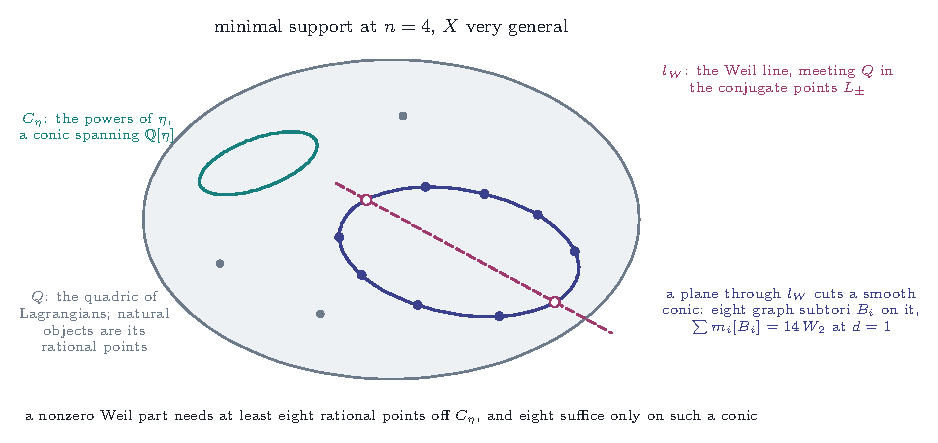
\includegraphics[width=0.94\textwidth]{fig_minimalsupport}
\caption{\Cref{thm:minimalsupport}. The quadric $Q$ of Lagrangians; the
rational points are the Chern characters of the natural objects on the split
member at $n=4$, up to the Veronese map $\nu_{4}$. The powers of the
polarisation fill the conic $C_{\eta}$ (teal), and the Weil line is spanned by
the conjugate points $L_{\pm}$ (open circles) in which the line $l_{W}$
(dashed) meets $Q$. A combination of natural characters with a nonzero Weil
part needs at least eight rational points off $C_{\eta}$, and with eight they
lie on one conic cut out by a plane through $l_{W}$ (indigo), such as the
eight graph subvarieties $B_{i}$ of \Cref{ex:fourteen}; the grey points are
natural objects off any such conic, which no relation of this size can use.}
\label{fig:minimalsupport}
\end{figure}

\begin{example}[Fourteen times a Weil class]\label{ex:fourteen}
Let $d=1$ and write $(\gamma-\sqrt{-1}\,\ell)^{4}=W_{1}+\sqrt{-1}\,W_{2}$ with
$W_{1},W_{2}$ rational, as in \Cref{thm:splitclosed}(iii). The eight
subvarieties $B_{i}=B_{(p_{i},q_{i})}$ with
\[
  (p_{i},q_{i})=(1,-3),\,(1,-2),\,(1,2),\,(1,3),\,(2,-1),\,(2,1),\,(3,-1),\,(3,1)
\]
and $m=(-1,16,-16,1,-16,16,1,-1)$ satisfy
\[
  \textstyle\sum_{i}m_{i}[B_{i}]=14\,W_{2},
\]
with the sign of $\varphi$ for which $B_{(p,q)}$ has conormal forms
$p\xi_{j}-qx_{n+j}$ and $p\xi_{n+j}+qx_{j}$; with the opposite sign the right
side is $-14W_{2}$. Among the $12870$ sets of eight subvarieties with
$|p|,|q|\le3$ this one has the least $\sum_{i}m_{i}^{2}$, namely $1028$, and
the least $\sum_{i}|m_{i}|$, namely $68$. In
general the coefficients of the relation of \Cref{thm:minimalsupport} for eight
subvarieties are proportional to
$\bigl((q_{i}^{2}+dp_{i}^{2})\prod_{j\ne i}(p_{i}q_{j}-p_{j}q_{i})\bigr)^{-1}$.
The sum $E=\bigoplus_{i}\cO_{B_{i}}^{\oplus|m_{i}|}[k_{i}]\oplus\cO(\eta)
\oplus\cO(2\eta)\oplus\cO(3\eta)$, with $k_{i}=0$ for $m_{i}>0$ and $1$
otherwise, has $\ch(E)=14W_{2}+\sum_{k}c_{k}\eta^{k}$ with
$k!\,c_{k}=1+2^{k}+3^{k}$, so $\rho=3$ and $r=104$, while
$\dim\Ext^{2}(E,E)=28868$; by \Cref{cor:naturalsums} it is far from the
criterion, and every direct sum of natural objects with $N\ne0$ has
$\dim\Ext^{2}\ge8\cdot28=224$.
\end{example}

\begin{remark}[The flatness form for direct sums]\label{rem:flatsums}
\Cref{lem:p2primesummands} does not apply to the flatness form of
\Cref{prop:p2flat}, but a direct sum fails that form too when its
cross-extensions cannot interact. Let $E=\bigoplus_{i}(\cO_{B_{i}}\otimes
L_{i})^{\oplus m_{i}}[k_{i}]$ with the $B_{i}$ pairwise distinct abelian
subvarieties of dimension $n$ meeting pairwise in finite sets, such as the
$B_{(p,q)}$. The extensions between different summands are concentrated in
degree $n$, so an arrow of $\Ext^{1}$ between summands raises the shift by
$n-1$, and a chain of $a\ge1$ arrows lands in $\Ext^{2+a(n-1)}\ne\Ext^{2}$.
Every term of the Maurer--Cartan equation that involves a cross-extension
therefore lands in a zero group, the base $K_{E}$ is the product of the
varieties of commuting $2n$-tuples of $m_{i}\times m_{i}$ matrices with the
space of cross-extensions, and a count of dimensions, using the
simultaneously diagonalisable component, gives $\dim K_{E}>e-k$; so (ii) and
(iii) of \Cref{prop:p2flat} fail. We give this in outline only. Indecomposable objects,
among them iterated extensions of at least eight natural blocks, and sums
whose cross-extensions compose to nonzero classes are not covered.
\end{remark}

\section{Secant objects on the split member}\label{sec:secantobjects}

\subsection{Sums of line bundles and the positivity obstruction}
\label{ssec:whatobject}

\Cref{thm:semiregclosure} asks for one perfect complex at one base point.
The cheapest candidate is a sum of line bundles on a split member, because
there the Weil classes are already polynomials in $\beta$, $\widehat\beta$ and
$\ell$ by \Cref{thm:splitclosed}, so the Chern character one wants is
manifestly in reach. This subsection settles that candidate. It does not
exist, and the obstruction is not semiregularity: it is the Chern character
condition, and it fails because the norm form of $K$ is positive
definite.

The norm rules out three different constructions in this paper, by three
different mechanisms, and they should be kept apart.
\Cref{thm:character} uses the norm \emph{character} of $\Kx$ and an
equivariance hypothesis. \Cref{prop:divfails} uses the fact that the part $R$
of $H^{2}$ on which $\Kx$ acts through $\tau^{2}$ and $\bbar\tau^{\,2}$ has no
Hodge classes at a general point, which is a statement about the Hodge group.
\Cref{thm:positivity} below uses neither: it uses that $\Nm_{K/\QQ}$ is a
positive definite quadratic form on $K$ and that the multiplicities of a
filtration are positive integers. The three are independent, and only the
third is available at a special point, which is exactly where the object of
\Cref{prop:ktheory} has to live.

\begin{lemma}[The semiregularity map of a split object]\label{lem:splitsemireg}
Let $Y$ be a smooth projective complex variety and let
\[
  E=\bigoplus_{i=1}^{s}L_{i}[p_{i}]^{\oplus m_{i}},
  \qquad \lambda_{i}=c_{1}(L_{i}),
\]
with the $L_{i}$ line bundles, the $\lambda_{i}$ pairwise distinct and
$p_{i}\in\ZZ$. Then for $\zeta=(\zeta_{ij})\in\Ext^{2}(E,E)$,
\begin{equation}\label{eq:splitsigma}
  \sigma_{E}(\zeta)_{q}
  =\frac{1}{q!}\sum_{i=1}^{s}(-1)^{p_{i}}\,
    \mathrm{tr}(\zeta_{ii})\,\lambda_{i}^{\,q},
\end{equation}
so $\sigma_{E}$ annihilates $\Ext^{2}(L_{i}[p_{i}],L_{j}[p_{j}])$ for $i\ne j$
and the traceless part of each diagonal block. Consequently $\sigma_{E}$ is
injective if and only if all three of the following hold:
\begin{enumerate}[label=\textup{(\roman*)},nosep]
\item $m_{i}=1$ for every $i$;
\item $H^{\,2+p_{i}-p_{j}}\bigl(Y,L_{j}L_{i}^{-1}\bigr)=0$ for all $i\ne j$;
\item the map
  \[
    \Phi\colon H^{2}(\cO_{Y})^{\oplus s}\longrightarrow H^{*}(Y,\CC),
    \qquad
    (\zeta_{i})\longmapsto\sum_{i}e^{\lambda_{i}}\zeta_{i},
  \]
  is injective.
\end{enumerate}
\end{lemma}

\begin{proof}
The Atiyah class of a direct sum is the direct sum of the Atiyah classes, and
that of a line bundle is its first Chern class, so $\mathrm{At}(E)$ is
diagonal with entries $\lambda_{i}$ and $\mathrm{At}(E)^{q}$ is diagonal with
entries $\lambda_{i}^{\,q}$. The matrix product $\zeta\circ\mathrm{At}(E)^{q}$
therefore has $(i,j)$ entry $\zeta_{ij}\lambda_{i}^{\,q}$, and the trace keeps
only the diagonal; a shift by $p$ multiplies the trace by $(-1)^{p}$. That is
\eqref{eq:splitsigma}, and it exhibits the two spaces the map kills.

For the equivalence, the off-diagonal part of $\Ext^{2}(E,E)$ is
$\bigoplus_{i\ne j}\Ext^{2}(L_{i}[p_{i}],L_{j}[p_{j}])
=\bigoplus_{i\ne j}H^{2+p_{i}-p_{j}}(L_{j}L_{i}^{-1})$, which must vanish,
giving (ii); the diagonal block at $i$ is $H^{2}(\cO_{Y})\otimes
\mathrm{End}(\CC^{m_{i}})$ and only its trace survives, so $m_{i}=1$, giving
(i). What is left is $\bigoplus_{i}H^{2}(\cO_{Y})$, and by
\eqref{eq:splitsigma} an element $(\zeta_{i})$ of it dies exactly when
$\sum_{i}\lambda_{i}^{\,q}\zeta_{i}=0$ for every $q\ge0$, which is (iii) after
absorbing the signs $(-1)^{p_{i}}$ into the $\zeta_{i}$ and the factorials
into the grading.
\end{proof}

Condition (ii) is cheap, because the shifts $p_{i}$ are at our disposal: only
their parities are fixed by the Chern character, and a line bundle whose first
Chern class is nondegenerate of index $k$ has cohomology in degree $k$ alone,
so one may choose the $p_{i}$ to avoid every index that occurs. Condition
(iii) is a rank condition, and condition (i) is free. What is not free is the
Chern character itself, and that is the subject of the rest of this
subsection.

\begin{notation}[Coordinates on the divisor classes]\label{not:splitcoords}
Let $A_{0}=X\times\widehat{X}$ be a split member, $n\ge2$, and keep
$\gamma=d\beta-\widehat{\beta}$ from \Cref{not:threeclasses}. Write
\[
  \theta^{\pm}=\gamma\mp\sqrt{-d}\,\ell\in\textstyle\bigwedge^{2}V_{\pm},
  \qquad
  R_{0}=\QQ\gamma\oplus\QQ\ell\subset R .
\]
Every $\theta\in R_{0}$ is $\theta=u\theta^{+}+\bbar u\,\theta^{-}$ for a
unique $u\in K$, and in coordinates $u=g+h\sqrt{-d}$ corresponds to
$\theta=2g\gamma+2dh\,\ell$. By \Cref{prop:splitgeom}(iv) the group
$\NS(A_{0})_{\QQ}$ at a split member with $X$ general is
$\QQ\eta\oplus R_{0}$, so every divisor class $\lambda$ is $e\eta+\theta$ with
$e\in\QQ$ and $\theta\in R_{0}$, and we write $u(\lambda)\in K$ for the
coordinate of its $R_{0}$-part.
\end{notation}

\begin{lemma}[A basis in degree four]\label{lem:sixmonomials}
For $n\ge2$ the six products
$\beta^{2},\widehat\beta^{2},\ell^{2},\beta\widehat\beta,\beta\ell,
\widehat\beta\ell$
are linearly independent in $H^{4}(A_{0},\QQ)$. Equivalently the six classes
$\eta^{2}$, $\eta\theta^{+}$, $\eta\theta^{-}$, $(\theta^{+})^{2}$,
$(\theta^{-})^{2}$, $\theta^{+}\theta^{-}$ are a basis of the degree four part
of the subring generated by the divisor classes.
\end{lemma}

\begin{proof}
Grade $H^{*}(A_{0},\QQ)=\bigwedge^{*}U\otimes\bigwedge^{*}U^{\vee}$ by
bidegree. Then $\beta$ has bidegree $(2,0)$, $\widehat\beta$ has $(0,2)$ and
$\ell$ has $(1,1)$, so the six products have bidegrees $(4,0)$, $(0,4)$,
$(2,2)$, $(2,2)$, $(3,1)$, $(1,3)$. All are distinct except for the pair
$\beta\widehat\beta$ and $\ell^{2}$, and those two are independent in
$\bigwedge^{2}U\otimes\bigwedge^{2}U^{\vee}$ because
$\beta\widehat\beta=\beta\otimes\widehat\beta$ is decomposable there while
$\ell^{2}=-2\sum_{i<j}(x_{i}x_{j})\otimes(\xi_{i}\xi_{j})$ is diagonal in
the induced bases, of tensor rank $\binom{2n}{2}>1$. The second
description follows because the change of basis between the two sets of six
classes is invertible over $K$: $\eta=d\beta+\widehat\beta$ and
$\gamma=d\beta-\widehat\beta$ span the same plane as
$\beta$ and $\widehat\beta$ since $\det\begin{psmallmatrix}d&1\\
d&-1\end{psmallmatrix}=-2d\ne0$, and $\theta^{\pm}$ span the same plane
as $\gamma$ and $\ell$ over $\CC$.
\end{proof}

The next lemma says the same thing at every abelian variety of Weil type, not
only at a split member, and it says it without coordinates. It is the fact on
which the positivity argument turns.

\begin{lemma}[$\theta^{+}\theta^{-}$ is never proportional to $\eta^{2}$]
\label{lem:tensorrank}
Let $(A,\iota,\eta)$ be of $(K,-1,n)$-Weil type with $n\ge2$, and let
$0\ne\theta^{\pm}\in\bigwedge^{2}V_{\pm}$. Then $\theta^{+}\theta^{-}$ is not a
scalar multiple of $\eta^{2}$ in $H^{4}(A,\CC)$.
\end{lemma}

\begin{proof}
Both classes lie in the summand
$\bigwedge^{2}V_{+}\otimes\bigwedge^{2}V_{-}$ of $H^{4}(A,\CC)$, the isotypic
component for the character $\Nm^{2}$, so the question is one of tensor rank
there. The polarisation class $\eta$ lies in $V_{+}\otimes V_{-}$ and is the
hermitian form of \Cref{prop:weilline}, hence nondegenerate: in dual bases
$\eta=\sum_{a=1}^{2n}v_{a}\wedge w_{a}$ with $v_{a}$ a basis of $V_{+}$ and
$w_{a}$ a basis of $V_{-}$. Squaring,
\[
  \eta^{2}
  =\sum_{a,b}(v_{a}\wedge w_{a})(v_{b}\wedge w_{b})
  =-2\sum_{a<b}(v_{a}v_{b})\otimes(w_{a}w_{b}),
\]
which is diagonal in the induced bases of $\bigwedge^{2}V_{+}$ and
$\bigwedge^{2}V_{-}$ and therefore has tensor rank exactly $\binom{2n}{2}$.
The class $\theta^{+}\theta^{-}$ is, up to sign,
$\theta^{+}\otimes\theta^{-}$, of tensor rank one. For $n\ge2$ one has
$\binom{2n}{2}\ge6>1$, so the two cannot be proportional.
\end{proof}

\begin{theorem}[The positivity obstruction]\label{thm:positivity}
Let $(A,\iota,\eta)$ be of $(K,-1,n)$-Weil type with $n\ge2$, and suppose that
the only divisor classes on which $\Kx$ acts through the norm character are
the multiples of $\eta$, that is
\begin{equation}\label{eq:noextranorm}
  \NS(A)_{\QQ}\cap\bigl(V_{+}\otimes V_{-}\bigr)=\QQ\,\eta .
\end{equation}
Let $E$ be a perfect complex on $A$ whose Chern character is effective in the
exponential basis, meaning
\begin{equation}\label{eq:effectivech}
  \ch(E)=\sum_{i=1}^{s}m_{i}\,e^{\lambda_{i}},
  \qquad m_{i}\in\QQ_{>0},\quad\lambda_{i}\in\NS(A)_{\QQ},
\end{equation}
and write $\lambda_{i}=e_{i}\eta+\theta_{i}$ with $\theta_{i}$ in the part $R$
of $H^{2}(A,\QQ)$ carrying the characters $\tau^{2}$ and $\bbar\tau^{\,2}$, and
$u_{i}\in K$ for the $\theta^{+}$-coordinate of $\theta_{i}$. If $\ch_{2}(E)$
is a flat Hodge class, then
\begin{equation}\label{eq:normsum}
  \sum_{i=1}^{s}m_{i}\,\Nm_{K/\QQ}(u_{i})=0 ,
\end{equation}
and since $\Nm_{K/\QQ}$ is positive definite and every $m_{i}$ is positive,
$u_{i}=0$ for every $i$. Hence every $\lambda_{i}$ is a rational multiple of
$\eta$, and $\ch_{k}(E)\in\QQ\,\eta^{k}$ for every $k$. In particular
$\ch_{n}(E)$ has no component on the Weil line.
\end{theorem}

\begin{proof}
From \eqref{eq:effectivech},
$\ch_{2}(E)=\tfrac12\sum_{i}m_{i}\lambda_{i}^{2}$, and hypothesis
\eqref{eq:noextranorm} is what makes the decomposition
$\lambda_{i}=e_{i}\eta+\theta_{i}$ available with $e_{i}$ a scalar. Decompose
$H^{4}(A,\CC)$ into $\Kx$-isotypic pieces and keep the one for $\Nm^{2}$,
namely $\bigwedge^{2}V_{+}\otimes\bigwedge^{2}V_{-}$. Writing
$\theta_{i}=u_{i}\theta^{+}+\bbar u_{i}\theta^{-}$ for a fixed choice of
generators $\theta^{\pm}$ of $\bigwedge^{2}V_{\pm}$, one has
\[
  \lambda_{i}^{2}
  =e_{i}^{2}\eta^{2}
   +2e_{i}\eta\theta_{i}
   +u_{i}^{2}(\theta^{+})^{2}+\bbar u_{i}^{2}(\theta^{-})^{2}
   +2\Nm_{K/\QQ}(u_{i})\,\theta^{+}\theta^{-},
\]
and of these five terms only the first and the last are in the $\Nm^{2}$
piece: $\eta\theta_{i}$ carries $\Nm\tau^{2}$ and $\Nm\bbar\tau^{\,2}$, and
$(\theta^{\pm})^{2}$ carry $\tau^{4}$ and $\bbar\tau^{\,4}$, all four distinct
from $\Nm^{2}$. So the $\Nm^{2}$-part of $\ch_{2}(E)$ is
\[
  \tfrac12\Bigl(\sum_{i}m_{i}e_{i}^{2}\Bigr)\eta^{2}
  +\Bigl(\sum_{i}m_{i}\Nm_{K/\QQ}(u_{i})\Bigr)\theta^{+}\theta^{-}.
\]

Now compare with the flat Hodge classes of degree four. For $n\ge3$ they are
$\QQ\eta^{2}$ by \Cref{thm:hdgcount}. For $n=2$ they are
$\QQ\eta^{2}\oplus\HW(A)$, and $\HW(A)$ spans the summands for $\tau^{4}$ and
$\bbar\tau^{\,4}$, which are not $\Nm^{2}$. In both cases the $\Nm^{2}$-part
of a flat Hodge class of degree four is a multiple of $\eta^{2}$. By
\Cref{lem:tensorrank} the class $\theta^{+}\theta^{-}$ is not such a multiple,
so its coefficient must vanish, which is \eqref{eq:normsum}.

Finally $\Nm_{K/\QQ}(g+h\sqrt{-d})=g^{2}+dh^{2}$ with $d>0$, so
$\Nm_{K/\QQ}(u)\ge0$ with equality only at $u=0$, and a sum of nonnegative
terms with positive weights vanishes only when every term does. Then
$\ch_{k}(E)=\frac{1}{k!}\bigl(\sum_{i}m_{i}e_{i}^{k}\bigr)\eta^{k}$, and
$\eta^{k}$ is not on the Weil line by \Cref{thm:hdgcount}.
\end{proof}

\begin{corollary}[Objects filtered by line bundles]\label{cor:nofiltered}
Let $A$ satisfy \eqref{eq:noextranorm}, which holds at every split member of
\Cref{thm:splitclosed} and at every quaternionic base point of
\Cref{thm:quatweil}. Then \Cref{thm:semiregclosure} cannot be applied at $A$
with any of the following:
\begin{enumerate}[label=\textup{(\alph*)},nosep]
\item a coherent sheaf admitting a filtration by line bundles, in particular
  any direct sum of line bundles;
\item a simple semi-homogeneous vector bundle in the sense of Mukai
  \cite{Muk78}, since such a bundle of rank $r$ has $\ch(E)=r\,e^{c_{1}(E)/r}$;
\item any iterated extension of the objects in (a) and (b).
\end{enumerate}
In each case the failure is not of the semiregularity hypothesis but of the
Chern character hypothesis of \Cref{prop:ktheory}: no such $E$ has a Chern
character which is a flat section of Hodge classes with a nonzero Weil
component.
\end{corollary}

\begin{proof}
First, \eqref{eq:noextranorm} holds at the points named. At a split member
$\NS(A)_{\QQ}$ has rank three with basis $\beta,\widehat\beta,\ell$ by
\Cref{prop:splitgeom}(iv), and of these $\eta$ spans the norm-character part
while $\gamma$ and $\ell$ span $R$. At a quaternionic point $\NS(A)_{\QQ}$ is
the space of Rosati-symmetric elements of $B=(-d,b)_{\QQ}$, which is spanned
by $1$, $j$ and $ij$; the first gives $\eta$ and the other two are semilinear
over $K$, hence lie in $R$. In both cases the norm-character part of
$\NS(A)_{\QQ}$ is exactly $\QQ\eta$.

Each of (a), (b) and (c) has a Chern character of the shape
\eqref{eq:effectivech} with positive multiplicities, by additivity of $\ch$
along a filtration and by Mukai's computation of the Chern character of a
simple semi-homogeneous bundle. The conclusion of \Cref{thm:positivity} then
contradicts the requirement that $\ch_{n}(E)$ have a nonzero component on the
Weil line.
\end{proof}

\begin{remark}[Scope of the theorem, and the objects of
Markman]\label{rem:markmanpositivity}
At a very general member of the family $\NS(A)_{\QQ}=\QQ\eta$, so
\Cref{thm:positivity} is true for the empty reason that there are no
$\theta_{i}$ to begin with. Its content is at the special members, which is
exactly where \Cref{thm:semiregclosure} needs its object to live and where the
base points of \Cref{thm:everyfamily} are. That is the opposite of the usual
situation in this paper, where the special members are the easy ones.

The theorem does not touch the objects of Markman \cite{Mar25a,Mar25b}.
Those are sheaves whose class in $K_{0}$ is not a positive combination of
exponentials of divisor classes, so \eqref{eq:effectivech} fails for them at
the first step; and they live at very general points, where, as just noted,
the statement is vacuous. What the theorem does is remove the class of
objects one would reach for first, and it removes it for a reason which is
visible before any cohomology is computed.
\end{remark}

\begin{remark}[Signed sums of line bundles]
\label{rem:whatitmustbe}
\Cref{thm:positivity} uses positivity of the multiplicities and nothing else,
so it says exactly where to go next: the object must be a complex whose
class in $K_{0}$ is not effective, that is one in which the line bundles
appear with multiplicities of both signs. Such objects exist. Writing
$E=F\oplus G[1]$ with $F$ and $G$ sums of line bundles, the class in $K_{0}$
is $[F]-[G]$ and \eqref{eq:normsum} becomes
$\sum_{L_{i}\subset F}\Nm(u_{i})=\sum_{L_{j}\subset G}\Nm(u_{j})$, which is
satisfiable; and \Cref{lem:splitsemireg} still applies verbatim, with the
shifts absorbing condition (ii).

The object of \Cref{thm:semiregclosure}, if it exists at a split member, is
not a sum of line bundles in any arrangement of signs and shifts:
\Cref{cor:noline} below proves this in every dimension. It must have
$\Ext^{2}$ that the trace does not see, that is, it must be indecomposable in
the derived category. This description of the remaining construction is
sharper than the one in \Cref{rem:tworemain}.
\end{remark}

\subsection{An explicit object and the Prouhet--Tarry--Escott problem}
\label{ssec:pte}

\Cref{prop:ktheory} produces the object of \Cref{thm:semiregclosure} by an
existence argument: the Chern character is an isomorphism onto the Chow ring
with rational coefficients, so a $K$-theory class with the right character
exists. That is enough for the theorem and tells one nothing about the object.
This subsection writes it down. The answer turns the question into a
Diophantine one, and the Diophantine problem has a classical name.

\begin{setupenv}[Objects supported on $R$]\label{setup:pte}
Let $A$ be of $(K,-1,n)$-Weil type, $n\ge2$, satisfying
\eqref{eq:noextranorm}, and keep $\theta^{\pm}$ from
\Cref{not:splitcoords}. For $u\in K$ with $\theta(u)=u\theta^{+}+\bbar
u\,\theta^{-}\in\NS(A)_{\QQ}$, and for multiplicities $m_{i}\in\ZZ$, consider
\[
  v=\sum_{i=1}^{s}m_{i}\,e^{\theta(u_{i})},
  \qquad
  T_{q,r}=\sum_{i=1}^{s}m_{i}\,u_{i}^{q}\,\bbar u_{i}^{\,r}
  \quad (q,r\ge0).
\]
\end{setupenv}

\begin{proposition}[The Chern character in terms of the $u_{i}$]
\label{prop:chintermsofu}
In \Cref{setup:pte},
\begin{equation}\label{eq:chexpansion}
  v_{k}
  =\sum_{\substack{q+r=k\\ 0\le q,r\le n}}
    \frac{T_{q,r}}{q!\,r!}\,(\theta^{+})^{q}(\theta^{-})^{r},
\end{equation}
because $(\theta^{\pm})^{q}=0$ for $q>n$. Consequently $v$ is a flat section
of Hodge classes with a nonzero Weil component if
\begin{equation}\label{eq:pteconditions}
  T_{q,r}=0\ \ \text{for all } 0\le q,r\le n \text{ with }
  (q,r)\notin\{(0,0),(n,0),(0,n)\},
  \qquad T_{n,0}\ne0,
\end{equation}
and then $v_{0}=T_{0,0}=\sum_{i}m_{i}$, $v_{k}=0$ for $0<k<2n$ with $k\ne n$,
and
\[
  v_{n}=\frac{1}{n!}\Bigl(T_{n,0}(\theta^{+})^{n}
        +\bbar{T}_{n,0}(\theta^{-})^{n}\Bigr),
\]
a nonzero rational multiple of a generator of the Weil line, by
\Cref{thm:splitclosed}.
\end{proposition}

\begin{proof}
Expand $\theta(u_{i})^{k}$ by the binomial theorem, divide by $k!$ and collect;
the vanishing of $(\theta^{\pm})^{q}$ for $q>n$ is because
$\theta^{\pm}\in\bigwedge^{2}V_{\pm}$ and $\dim_{\CC}V_{\pm}=2n$. Under
\eqref{eq:pteconditions} the only surviving terms of \eqref{eq:chexpansion}
are the ones listed, and $(\theta^{+})^{n}$ spans $\bigwedge^{2n}V_{+}$, which
is the Weil line over $\CC$.
\end{proof}

So the search for the object of \Cref{thm:semiregclosure} is the search for a
finitely supported integer-valued function on $\cO_{K}$ that annihilates every
monomial $u^{q}\bbar u^{\,r}$ with $q,r\le n$ except three of them. Two things
follow at once, and they pull in opposite directions.

\begin{lemma}[Equal norms force the Prouhet--Tarry--Escott condition]
\label{lem:pte}
Suppose all the $u_{i}$ in \Cref{setup:pte} have the same norm
$N=\Nm_{K/\QQ}(u_{i})>0$. Then \eqref{eq:pteconditions} holds if and only if
\begin{equation}\label{eq:ptepure}
  \sum_{i}m_{i}u_{i}^{\,k}=0\ \ \text{for } k=0,1,\dots,n-1,
  \qquad
  \sum_{i}m_{i}u_{i}^{\,n}\ne0 .
\end{equation}
With $m_{i}=\pm1$ this says that the $u_{i}$ split into two multisets on the
circle $\Nm=N$ whose power sums agree through degree $n-1$ and differ at
degree $n$: a Prouhet--Tarry--Escott pair of degree $n-1$, constrained to a
norm circle of $\cO_{K}$.
\end{lemma}

\begin{proof}
For $q\ge r$ one has $u^{q}\bbar u^{\,r}=N^{r}u^{q-r}$, so
$T_{q,r}=N^{r}\sum_{i}m_{i}u_{i}^{\,q-r}$, and the pairs $(q,r)$ with
$q,r\le n$ realise every difference $k=q-r$ from $0$ to $n$. The excluded
pairs $(0,0)$ and $(n,0)$ are the ones with $r=0$ and $k=0$ or $k=n$; but
$k=0$ also occurs at $(1,1),\dots,(n,n)$, which are not excluded, so
$\sum_{i}m_{i}=0$ is still required. The remaining differences
$k=1,\dots,n-1$ each occur at some non-excluded pair, and $k=n$ occurs only at
$(n,0)$.
\end{proof}

\begin{theorem}[Equal norms cannot be semiregular]\label{thm:equalnorms}
Let $E=\bigoplus_{i}L_{i}[p_{i}]$ realise \eqref{eq:ptepure} with all norms
equal. Then $\ch_{0}(E)=0$, and the semiregularity map $\sigma_{E}$ has a
kernel of dimension at least $n^{2}$.
\end{theorem}

\begin{proof}
By \Cref{lem:pte} the case $k=0$ of \eqref{eq:ptepure} gives
$\sum_{i}m_{i}=0$, which is $\ch_{0}(E)$. For the kernel, take
$\zeta_{i}=m_{i}\zeta$ for a single $\zeta\in H^{2}(\cO_{A})$; then by
\Cref{lem:splitsemireg}(iii)
\[
  \Phi\bigl((m_{i}\zeta)_{i}\bigr)
  =\Bigl(\sum_{i}m_{i}e^{\lambda_{i}}\Bigr)\zeta=\ch(E)\,\zeta ,
\]
which by \Cref{prop:chintermsofu} is a multiple of $\omega\,\zeta$ with
$\omega$ a generator of the Weil line. Now $\HW(A)_{\CC}$ is spanned by
$\bigwedge^{2n}V_{+}$ and $\bigwedge^{2n}V_{-}$, and the Weil type condition
says $\dim V_{\pm}^{0,1}=n$; writing
$H^{2}(\cO_{A})=\bigwedge^{2}(V_{+}^{0,1}\oplus V_{-}^{0,1})$, the product of
a generator of $\bigwedge^{2n}V_{+}$ with $\zeta$ kills the components of
$\zeta$ in $\bigwedge^{2}V_{+}^{0,1}$ and in
$V_{+}^{0,1}\otimes V_{-}^{0,1}$, and likewise with the roles exchanged. So
$\omega\,\zeta=0$ for every $\zeta$ in
$V_{+}^{0,1}\otimes V_{-}^{0,1}$, a space of dimension $n^{2}$, and all of
those lie in the kernel of $\Phi$.
\end{proof}

\begin{corollary}[At least $n+1$ norms]\label{cor:nplusone}
If $E$ as in \Cref{setup:pte} satisfies \eqref{eq:pteconditions} and
$\ch_{0}(E)\ne0$, then the $u_{i}$ take at least $n+1$ distinct norms.
\end{corollary}

\begin{proof}
Let $N_{1},\dots,N_{\nu}$ be the distinct norms and $M_{j}$ the sum of the
$m_{i}$ over the level $\Nm(u_{i})=N_{j}$. The conditions $T_{r,r}=0$ for
$r=1,\dots,n$ read $\sum_{j}M_{j}N_{j}^{\,r}=0$ for $r=1,\dots,n$. The matrix
$(N_{j}^{\,r})_{1\le r\le n,\,1\le j\le\nu}$ has rank $\min(n,\nu)$ because the
$N_{j}$ are distinct and nonzero, so $\nu\le n$ forces every $M_{j}=0$ and
hence $\ch_{0}(E)=\sum_{j}M_{j}=0$.
\end{proof}

\subsubsection*{The smallest solution}

At $n=3$ and $K=\QQ(\sqrt{-3})$ the Prouhet--Tarry--Escott condition of
\Cref{lem:pte} has a particularly simple solution: the norm circle
$\Nm=1$ carries the six roots of unity of $K$, and the two cosets of the cube
roots of $-1$ and of $+1$ are a Prouhet--Tarry--Escott pair of degree
two. Explicitly, with $\zeta_{6}$ a primitive sixth root of unity, the
cube roots of $-1$ are $\zeta_{6},\zeta_{6}^{3},\zeta_{6}^{5}$ and those of
$+1$ are $1,\zeta_{6}^{2},\zeta_{6}^{4}$; each triple sums to zero and has
zero sum of squares,
while the sums of cubes are $-3$ and $+3$.

\begin{proposition}[An explicit object at $n=3$]\label{prop:explicitobject}
Let $K=\QQ(\sqrt{-3})$, $n=3$, and let $A_{0}=X\times\widehat X$ be a split
member. In the basis $\beta,\widehat\beta,\ell$ of $\NS(A_{0})_{\QQ}$ put
\[
  \lambda_{1}=(3,-1,3),\quad
  \lambda_{2}=(-6,2,0),\quad
  \lambda_{3}=(3,-1,-3),
\]
and $\lambda_{3+i}=-\lambda_{i}$ for $i=1,2,3$, with $m_{i}=+1$ for
$i\le3$ and $m_{i}=-1$ for $i\ge4$. Then the six classes are distinct and
integral, the perfect complex
\[
  E=\bigl(L_{1}\oplus L_{2}\oplus L_{3}\bigr)\ \oplus\
    \bigl(L_{4}\oplus L_{5}\oplus L_{6}\bigr)[3]
\]
has
\[
  \ch_{k}(E)=0\ \ (k\ne3),
  \qquad
  \ch_{3}(E)=12\,\omega_{1},
\]
and every difference $\lambda_{j}-\lambda_{i}$ with $i\ne j$ is nondegenerate
of index exactly $3$, so that conditions (i) and (ii) of
\Cref{lem:splitsemireg} hold for this shift. Condition (iii) fails: the map
$\Phi$ has rank $75$ instead of $90$, with kernel of dimension
$15=\dim H^{2}(\cO_{A_{0}})$.
\end{proposition}

\begin{proof}
With $d=3$, the class $\theta(u)=2g\gamma+6h\ell$ of $u=g+h\sqrt{-3}$ has
coordinates $(6g,-2g,6h)$, so $\lambda_{1},\lambda_{2},\lambda_{3}$ are the
images of the cube roots $\zeta_{6},\zeta_{6}^{3},\zeta_{6}^{5}$ of $-1$ and
$\lambda_{4},\lambda_{5},\lambda_{6}$ those of the cube roots of $+1$; the six
classes are distinct and integral. All six have norm $1$, and
$\sum_{i}m_{i}u_{i}^{k}$ is $0$ for $k=0,1,2$ and $-3-3=-6$ for $k=3$, so
\eqref{eq:ptepure} holds at $n=3$. By \Cref{lem:pte} and
\Cref{prop:chintermsofu}, $\ch_{k}(E)=0$ for $k\ne3$ and
$\ch_{3}(E)=-\bigl((\theta^{+})^{3}+(\theta^{-})^{3}\bigr)$, and by
\Cref{ex:splitsmall} at $n=3$,
$\omega_{1}\pm\sqrt{-3}\,\omega_{2}=-\frac16(\theta^{\mp})^{3}$; so
$\ch_{3}(E)=12\,\omega_{1}$.

Every difference is $\lambda_{j}-\lambda_{i}=\theta(w)$ with
$w=u_{j}-u_{i}\ne0$, and $\theta(w)$ is nondegenerate of index $n$ for every
$w\in K^{\times}$. Indeed $\theta(1)=2\gamma$ and $\theta(\sqrt{-d})=2d\ell$ are of
type $(1,1)$, hence so are $\theta^{\pm}$, so
$\theta^{+}\in V_{+}^{1,0}\otimes V_{+}^{0,1}$, and $V_{+}^{0,1}$ is the
conjugate of $V_{-}^{1,0}$. In the splitting of the tangent space dual to
$H^{1,0}=V_{+}^{1,0}\oplus V_{-}^{1,0}$, the hermitian form of $\theta(w)$
therefore has the block form
$\bigl(\begin{smallmatrix}0&wP\\ \bar wP^{*}&0\end{smallmatrix}\bigr)$, with $P$
the block of $2\gamma$, which is invertible because $\gamma$ is nondegenerate.
Its eigenvalues are plus and minus the singular values of $wP$, so it has
signature $(n,n)$, and a line bundle with this class has cohomology only in
degree $n$ \cite[Chapter~3]{BL04}. For the shift, condition (ii) asks that
$2+p_{i}-p_{j}\ne3$ whenever $i\ne j$, that is $p_{i}-p_{j}\ne1$; within each
of the two blocks the difference is $0$, and between them it is $\pm3$.

For the rank, the $u_{i}$ are the six sixth roots of unity, each once, and
$\bbar u_{i}=u_{i}^{-1}$. Absorb the signs into the $\zeta_{i}$ as in
\Cref{lem:splitsemireg}(iii) and expand
$e^{\lambda_{i}}=e^{u_{i}\theta^{+}}e^{\bbar u_{i}\theta^{-}}$:
\[
  \Phi(\zeta)=\sum_{a,b=0}^{3}\frac{(\theta^{+})^{a}(\theta^{-})^{b}}{a!\,b!}\,Z_{a-b},
  \qquad Z_{k}=\sum_{i}u_{i}^{k}\zeta_{i},
\]
with $k$ read modulo $6$. The $Z_{0},\dots,Z_{5}$ determine the $\zeta_{i}$,
by a Vandermonde matrix. Split
$H^{0,2}(A_{0})=\bigwedge^{2}V_{+}^{0,1}\oplus(V_{+}^{0,1}\otimes V_{-}^{0,1})
\oplus\bigwedge^{2}V_{-}^{0,1}$, write $Z_{k}=Z_{k}^{+}+Z_{k}^{0}+Z_{k}^{-}$
accordingly, and grade $H^{*}(A_{0})=\bigwedge^{*}V_{+}\otimes\bigwedge^{*}V_{-}$
by the Hodge types of the two factors. The term
$(\theta^{+})^{a}(\theta^{-})^{b}Z_{k}^{0}$ has types $(a,a+1)$ and $(b,b+1)$,
the term with $Z_{k}^{+}$ has types $(a,a+2)$ and $(b,b)$, and the term with
$Z_{k}^{-}$ has types $(a,a)$ and $(b,b+2)$. These are different for
different $(a,b)$ and different pieces, so every term vanishes separately.
Since $\theta^{\pm}$ pairs $V_{\pm}^{1,0}$ nondegenerately with $V_{\pm}^{0,1}$,
both of dimension $3$, multiplication by $(\theta^{\pm})^{a}$ is injective on
$\bigwedge^{j}V_{\pm}^{0,1}$ when $a+j\le3$ and zero otherwise; in bases
with $\theta^{+}=\sum_{i}e_{i}f_{i}$ it sends $f_{J}$ to a signed sum of the
$e_{I}f_{I\cup J}$ with $I\cap J=\emptyset$, $|I|=a$, and different $J$ give
disjoint supports. Hence $Z_{k}^{0}=0$ unless no $a,b\le2$ have $a-b\equiv k$,
which leaves $k=3$; $Z_{k}^{+}=0$ unless no $a\le1$, $b\le3$ have
$a-b\equiv k$, which leaves $k=2$; and likewise $Z_{k}^{-}=0$ unless $k=4$. So
$\ker\Phi$ is $V_{+}^{0,1}\otimes V_{-}^{0,1}$ at $k=3$ together with
$\bigwedge^{2}V_{+}^{0,1}$ at $k=2$ and $\bigwedge^{2}V_{-}^{0,1}$ at $k=4$, of
dimension $9+3+3=15=\dim H^{2}(\cO_{A_{0}})$, and $\Phi$ has rank
$90-15=75$. The first summand is the kernel of \Cref{thm:equalnorms}.
\end{proof}

\begin{remark}[What the construction settles]\label{rem:pteoutcome}
Three things are settled. The object of \Cref{prop:ktheory} is not an
abstraction: at $n=3$ over $\QQ(\sqrt{-3})$ it is six line bundles and a
shift, and its Chern character is exactly $12$ times a Weil class with every
other graded piece zero. The construction is completely general, and
\Cref{lem:pte} identifies the constraint as a Prouhet--Tarry--Escott problem
on a norm circle, a question of a kind that can be attacked directly. And
\Cref{cor:nplusone} says what any semiregular solution must look like: the
$u_{i}$ must take at least $n+1$ distinct norms, because otherwise the rank is
zero and the argument of \Cref{thm:equalnorms} produces a kernel of
dimension $n^{2}$.

This leaves the existence of a solution with $n+1$ norms. The level sums are
then forced up to scale (\Cref{thm:pterange}), and \Cref{cor:noline} shows
that no solution could serve, because a line bundle summand off the
polarisation line is obstructed along the family whatever the norms.
\end{remark}

\subsubsection*{The obstruction classes of the explicit object}

\Cref{cor:kernelfamily} and \Cref{rem:whatmeasures} say that the kernel of
$\sigma_{E}$ contains a copy of the tangent space of the Weil family, and
that this is a statement about where the semiregularity map is blind, not a
statement that the object is obstructed. For the explicit object the
obstruction classes can be written down, and they are not zero. The
computation is elementary and we record it in general.

Recall the conventions of \Cref{ssec:tangent}: a first-order deformation of
$A$ is $v\in\Hom(H^{1,0},H^{0,1})=H^{1}(A,T_{A})$, extended by zero on
$H^{0,1}$ and acting on $H^{*}(A,\CC)$ as a derivation $v\lrcorner$; a class
$\xi$ of type $(p,p)$ stays of type $(p,p)$ to first order along $v$ exactly
when $v\lrcorner\,\xi=0$. For a line bundle $L$ with $\lambda=c_{1}(L)$ the
Atiyah class is $\lambda\in H^{1}(\Omega^{1}_{A})$, its contraction with $v$
is $v\lrcorner\,\lambda\in H^{2}(\cO_{A})=H^{0,2}(A)$, and this is the
obstruction to deforming $L$ along $v$; a shift does not change it. For
$E=\bigoplus_{i}L_{i}[p_{i}]$ the Atiyah class is diagonal with entries
$\lambda_{i}$, as in the proof of \Cref{lem:splitsemireg}, so the
obstruction to deforming $E$ along $v$ is the diagonal element
\begin{equation}\label{eq:obdef}
  \ob_{E}(v)=\bigl(v\lrcorner\,\lambda_{i}\bigr)_{i}
  \in\bigoplus_{i}H^{0,2}(A)\subset\Ext^{2}(E,E).
\end{equation}

\begin{proposition}[The obstruction map of a split object]
\label{prop:splitobstruction}
Let $A_{0}=X\times\widehat X$ be a split member with $\beta$ principal and
$X$ general, so that $\NS(A_{0})_{\QQ}=\langle\beta,\widehat\beta,\ell\rangle$
by \Cref{prop:splitgeom}(iv). Let $T=T_{[A_{0}]}\cD_{n,n}$ be the space of
polarised first-order deformations commuting with $K$, of dimension $n^{2}$
by \Cref{prop:firstorder}, and put
\[
  T_{\mathrm{spl}}
  =\bigl\{\,v\in\Hom(H^{1,0},H^{0,1})\;:\;
    v\lrcorner\,\beta=v\lrcorner\,\widehat\beta=v\lrcorner\,\ell=0\,\bigr\}.
\]
Let $E=\bigoplus_{i=1}^{s}L_{i}[p_{i}]$ with $\lambda_{i}=c_{1}(L_{i})$ and
let $\ob_{E}\colon T\to\bigoplus_{i}H^{0,2}(A_{0})$ be the map
\eqref{eq:obdef} restricted to $T$.
\begin{enumerate}[label=\textup{(\roman*)},nosep]
\item $T_{\mathrm{spl}}$ is the tangent space to the split locus: it has
  dimension $n(n+1)/2$, it is contained in $T$, and it consists of the
  deformations of $X\times\widehat X$ induced by the polarised deformations
  of $(X,\beta)$.
\item If the classes $\lambda_{i}$ together with $\eta$ span
  $\NS(A_{0})_{\QQ}$, then $\ker\ob_{E}=T_{\mathrm{spl}}$ and
  $\operatorname{rank}\ob_{E}=n(n-1)/2$, the codimension of the split locus
  in $\cD_{n,n}$.
\item If $\ch_{k}(E)\in\QQ\eta^{k}$ for $k\ne n$ and
  $\ch_{n}(E)\in\QQ\eta^{n}\oplus\HW(A_{0})$, then
  $\sigma_{E}\circ\ob_{E}=0$ on $T$: for every $v\in T$,
  \begin{equation}\label{eq:sigmaob}
    \sigma_{E}\bigl(\ob_{E}(v)\bigr)=v\lrcorner\,\ch(E)=0 .
  \end{equation}
\item For the object of \Cref{prop:explicitobject}, at $n=3$ and
  $K=\QQ(\sqrt{-3})$: $\ker\ob_{E}=T_{\mathrm{spl}}$ has dimension $6$ and
  $\ob_{E}$ has rank $3$; the image of $\ob_{E}$ lies in $\ker\sigma_{E}$;
  the subspace $\Delta=\{z\cdot\id_{E}:z\in\Ann_{H^{0,2}}(\omega_{1})\}$ of
  \Cref{cor:kernelfamily} has dimension $9$ and meets the image of $\ob_{E}$
  only in zero, so that $\Delta\oplus\image\ob_{E}$ is a twelve-dimensional
  subspace of the fifteen-dimensional kernel of $\sigma_{E}$; and
  $\ob_{E}(v)$ has components $v\lrcorner\,\lambda_{i}$ on $L_{i}$ and
  $-v\lrcorner\,\lambda_{i}$ on $L_{i}^{-1}[3]$, so it lies on the line of
  vectors of the shape $(z,\dots,z)$ only when it vanishes. In particular
  $E$ has a nonzero first-order obstruction along every $v\in T$ not tangent
  to the split locus, and no element $z\cdot\id_{E}$ of $\Ext^{2}(E,E)$
  cancels it.
\end{enumerate}
\end{proposition}

\begin{proof}
(i) Let $P=H^{1,0}(X)\subset H^{1}(X,\CC)=U^{\vee}_{\CC}$ with basis
$p_{1},\dots,p_{n}$, so that $p_{1},\dots,p_{n},\bbar p_{1},\dots,\bbar p_{n}$
is a basis of $U^{\vee}_{\CC}$, and let $q_{a},\bbar q_{a}$ be the dual basis
of $U_{\CC}=H^{1}(\widehat X,\CC)$; the dual of a conjugate basis is the
conjugate of the dual basis, so the notation is consistent. The Poincar\'e
class is the identity element of $U^{\vee}\otimes U$,
\[
  \ell=\sum_{a=1}^{n}\bigl(p_{a}\wedge q_{a}+\bbar p_{a}\wedge\bbar q_{a}\bigr),
\]
and it is of type $(1,1)$, which forces $H^{1,0}(\widehat X)=\langle\bbar
q_{a}\rangle$ and $H^{0,1}(\widehat X)=\langle q_{a}\rangle$: the Hodge
structure of $\widehat X$ is the dual one. Since $\beta$ is of type $(1,1)$
and nondegenerate, $\beta=\sum_{a,b}h_{ab}\,p_{a}\wedge\bbar p_{b}$ with
$h\in\GL_{n}(\CC)$; and since $\beta$ is principal with Gram matrix $B$ in a
symplectic basis of $U$ and $\widehat\beta$ has Gram matrix $-B^{-1}=B$ in
the dual basis of $U^{\vee}$, the Gram matrix of $\widehat\beta$ in the
basis $p_{a},\bbar p_{a}$ is minus the inverse of the Gram matrix
$\begin{psmallmatrix}0&h\\-h^{\top}&0\end{psmallmatrix}$ of $\beta$ in the
basis $q_{a},\bbar q_{a}$, which gives
$\widehat\beta=-\sum_{a,b}(h^{-1})_{ab}\,\bbar q_{a}\wedge q_{b}$.

Now $H^{1,0}(A_{0})=\langle p_{a}\rangle\oplus\langle\bbar q_{a}\rangle$ and
$H^{0,1}(A_{0})=\langle\bbar p_{a}\rangle\oplus\langle q_{a}\rangle$, so a
deformation $v$ is four $n\times n$ matrices,
\[
  v(p_{a})=\sum_{c}\bigl(A_{ca}\,\bbar p_{c}+C_{ca}\,q_{c}\bigr),
  \qquad
  v(\bbar q_{a})=\sum_{c}\bigl(B_{ca}\,\bbar p_{c}+D_{ca}\,q_{c}\bigr),
\]
and $v$ kills $\bbar p_{a}$ and $q_{a}$. Contracting,
\[
  v\lrcorner\,\ell
  =\sum_{a,c}\Bigl(A_{ca}\,\bbar p_{c}\wedge q_{a}+C_{ca}\,q_{c}\wedge q_{a}
   +B_{ca}\,\bbar p_{a}\wedge\bbar p_{c}+D_{ca}\,\bbar p_{a}\wedge q_{c}\Bigr),
\]
and reading off the three kinds of monomials, $v\lrcorner\,\ell=0$ if and only
if $D=-A^{\top}$ and $B$, $C$ are symmetric. Next
\[
  v\lrcorner\,\beta
  =\sum_{a,b,c}h_{ab}\Bigl(A_{ca}\,\bbar p_{c}\wedge\bbar p_{b}
   +C_{ca}\,q_{c}\wedge\bbar p_{b}\Bigr),
\]
so $v\lrcorner\,\beta=0$ if and only if $Ch=0$, that is $C=0$, and $Ah$ is
symmetric. Likewise $v\lrcorner\,\widehat\beta=0$ if and only if $B=0$ and
$Dh^{-1}$ is symmetric. Given $D=-A^{\top}$, the last condition reads
$A^{\top}h^{-1}=h^{-\top}A$, which after multiplication by $h^{\top}$ on the
left and by $h$ on the right is $h^{\top}A^{\top}=Ah$, the symmetry of $Ah$
again. Hence
\[
  T_{\mathrm{spl}}=\bigl\{(A,B,C,D)=(A,0,0,-A^{\top})\;:\;Ah\ \text{symmetric}\bigr\},
\]
of dimension $n(n+1)/2$. It is the tangent space to the split locus: the
same computation on $X$ alone shows that the polarised first-order
deformations of $(X,\beta)$ are the matrices $A$ with $Ah$ symmetric, the
space $T_{[X]}\cA_{n}$ of dimension $n(n+1)/2$; the deformation of
$\widehat X$ induced by $A$ is the dual one, $-A^{\top}$; and the map
$A\mapsto(A,0,0,-A^{\top})$ is injective. Finally $T_{\mathrm{spl}}\subseteq
T$: for $v\in T_{\mathrm{spl}}$, $v\lrcorner\,\eta=0$ because
$\eta\in\langle\beta,\widehat\beta\rangle$, so $v$ is polarised, and
$v\lrcorner\,\omega_{1}=v\lrcorner\,\omega_{2}=0$ because $\omega_{1}$ and
$\omega_{2}$ are polynomials in $\beta,\widehat\beta,\ell$ by
\Cref{thm:splitclosed} and $v\lrcorner$ is a derivation; by
\Cref{prop:firstorder} such a $v$ commutes with $K$.

(ii) Every $v\in T$ has $v\lrcorner\,\eta=0$. If the $\lambda_{i}$ and
$\eta$ span $\NS(A_{0})_{\QQ}=\langle\beta,\widehat\beta,\ell\rangle$, then
$v\lrcorner\,\lambda_{i}=0$ for all $i$ is equivalent, for $v\in T$, to
$v\lrcorner\,\beta=v\lrcorner\,\widehat\beta=v\lrcorner\,\ell=0$, so
$\ker\ob_{E}=T\cap T_{\mathrm{spl}}=T_{\mathrm{spl}}$ by (i), and the rank
is $n^{2}-n(n+1)/2=n(n-1)/2$, which is the codimension of
\Cref{prop:splitgeom}(iii).

(iii) By \eqref{eq:splitsigma}, $\sigma_{E}(\zeta)=\sum_{i}(-1)^{p_{i}}
\zeta_{ii}\,e^{\lambda_{i}}$ for a diagonal $\zeta$. Since $v\lrcorner$ is a
derivation and $v\lrcorner\,\lambda_{i}$ has even degree,
$v\lrcorner\,\lambda_{i}^{\,q}=q\,\lambda_{i}^{\,q-1}(v\lrcorner\,\lambda_{i})$
and so $v\lrcorner\,e^{\lambda_{i}}=(v\lrcorner\,\lambda_{i})\,e^{\lambda_{i}}$.
Therefore
\[
  \sigma_{E}\bigl(\ob_{E}(v)\bigr)
  =\sum_{i}(-1)^{p_{i}}(v\lrcorner\,\lambda_{i})\,e^{\lambda_{i}}
  =v\lrcorner\sum_{i}(-1)^{p_{i}}e^{\lambda_{i}}
  =v\lrcorner\,\ch(E).
\]
For $v\in T$ one has $v\lrcorner\,\eta^{k}=k\eta^{k-1}(v\lrcorner\,\eta)=0$,
and $v\lrcorner\,\omega=0$ for every $\omega\in\HW(A_{0})$ by
\Cref{prop:firstorder}; under the hypothesis on $\ch(E)$ this gives
\eqref{eq:sigmaob}.

(iv) The three classes $\lambda_{1}=\gamma+3\ell$, $\lambda_{2}=-2\gamma$,
$\lambda_{3}=\gamma-3\ell$ span $\langle\gamma,\ell\rangle$, and
$\langle\eta,\gamma\rangle=\langle\beta,\widehat\beta\rangle$ by the
determinant in the proof of \Cref{lem:sixmonomials}, so (ii) applies and
gives the kernel and the rank; \Cref{prop:explicitobject} gives the
hypothesis of (iii), so the image lies in $\ker\sigma_{E}$. The subspace
$\Delta$ has dimension $\dim\Ann_{H^{0,2}}(\omega_{1})=n^{2}=9$ by
\Cref{lem:annihilator}. The components of $\ob_{E}(v)$ on $L_{i}$ and on
$L_{i}^{-1}[3]$ are $v\lrcorner\,\lambda_{i}$ and
$v\lrcorner\,(-\lambda_{i})=-v\lrcorner\,\lambda_{i}$, so an element of the
image of the shape $(z,\dots,z)$ has $z=-z$, hence is zero; this is
$\Delta\cap\image\ob_{E}=0$, and with $\dim\ker\sigma_{E}=15$ from
\Cref{prop:explicitobject} the dimension count follows.
\end{proof}

\begin{remark}[Meaning of the obstruction classes]\label{rem:obstructionmeaning}
\Cref{prop:splitobstruction} sharpens \Cref{rem:whatmeasures} in one
respect and exposes a limit of the criterion in another. First, for the
explicit object the obstruction classes along the family are nonzero, and
they are nonzero exactly in the $n(n-1)/2$ directions normal to the split
locus, which are the directions in which the Weil class has to be
transported. Second, those classes lie in the kernel of $\sigma_{E}$ by
\eqref{eq:sigmaob}, and \eqref{eq:sigmaob} holds for every object whose
Chern character is a flat section of Hodge classes along the family, so the
semiregularity map cannot detect the obstruction of any such object. The
obstruction is therefore nonzero, and the criterion cannot see it. For
the explicit object the
situation is the worst possible: the twelve dimensions
$\Delta\oplus\image\ob_{E}$ of the kernel are accounted for by the two
mechanisms of \Cref{cor:kernelfamily} and \eqref{eq:obdef}, the remaining
three lie on the even side of \Cref{cor:pteobstructed} as well, and none of
the fifteen is an artefact. The classes of the shape $z\cdot\id_{E}$ are the
ones a change of the twisting class would contribute, one and the same $z$
to every rank one summand; the last assertion of (iv) says that no such
change removes the obstruction. So the explicit object does not move off the
split locus to first order, either as a complex or as a twisted complex, and
the question of \Cref{q:residual} for it is not one of verifying a
hypothesis but of replacing the object.

The positive content is a recipe. By (ii), a split object whose classes
span $\NS(A_{0})_{\QQ}$ with $\eta$ has obstruction map of rank
$n(n-1)/2$ against the family, and the spanning hypothesis is more than is
needed: a single class $\theta\in\NS(A_{0})_{\QQ}$ not proportional to
$\eta$ already has $\{v\in T:v\lrcorner\,\theta=0\}=T_{\mathrm{spl}}$.
Indeed, every $v\in T$ kills $\eta$ and commutes with $K$, so it is a pair
$(v_{+},v_{-})$ with $v_{\pm}\in\Hom(V_{\pm}^{1,0},V_{\pm}^{0,1})$. Since
$\theta^{\pm}$ is of type $(1,1)$ in $\bigwedge^{2}V_{\pm}$, the $R_{0}$-part
$u\theta^{+}+\bbar u\,\theta^{-}$ of $\theta$, with $u\ne0$, gives
$v\lrcorner\,\theta=u\,v_{+}\lrcorner\,\theta^{+}+\bbar u\,v_{-}\lrcorner\,\theta^{-}$,
whose two terms lie in the different summands $\bigwedge^{2}V_{+}^{0,1}$ and
$\bigwedge^{2}V_{-}^{0,1}$ of $H^{0,2}(A_{0})$. So the kernel of
$v\mapsto v\lrcorner\,\theta$ on $T$ does not depend on $u\ne0$; it is
therefore the common kernel for $\gamma$ and $\ell$, the cases $u=1$ and
$u=\sqrt{-d}$, which is $T_{\mathrm{spl}}$ by (ii). So every split object built from line bundles
other than powers of $\eta$ is obstructed in exactly the normal directions
to the split locus, and \Cref{thm:positivity} says that an object built
from powers of $\eta$ carries no Weil class. What survives is the statement
of \Cref{rem:familyuniform}: the object must have positive rank.
\end{remark}

\subsubsection*{The evaluation map of the explicit object}

\Cref{thm:weakfails} places the copy $\Delta$ of the tangent space inside the
image of the evaluation map. For a split object the whole of
$\operatorname{ev}_{E}$ can be written down, and for the explicit object the
entire kernel of $\sigma_{E}$ turns out to lie in its image. We identify
$HH^{2}(A_{0})$ with
\begin{equation}\label{eq:HT2}
  HT^{2}(A_{0})
  =H^{0,2}(A_{0})\;\oplus\;\Hom\bigl(H^{1,0},H^{0,1}\bigr)\;\oplus\;
   \textstyle\bigwedge^{2}\bigl(H^{1,0}\bigr)^{\vee}
\end{equation}
by the Hochschild--Kostant--Rosenberg isomorphism, the three summands being
$H^{2}(\cO)$, $H^{1}(T)$ and $H^{0}(\bigwedge^{2}T)$ for the trivial tangent
bundle. An element $x=(z,v,\pi)$ acts on $H^{*}(A_{0},\CC)$ by $z\wedge$, by
the derivation $v\lrcorner$ of \Cref{ssec:tangent}, and by the double
contraction $\pi\lrcorner$, which removes two $(1,0)$ slots; we write
$x\lrcorner\,\xi$ for the sum of the three.

The double contraction is a second order operator. For a class $\lambda$ of
type $(1,1)$, which has a single $(1,0)$ slot, $\pi\lrcorner\,\lambda=0$ and
$\pi\lrcorner\,\lambda^{k}=\binom{k}{2}\lambda^{k-2}\,(\pi\lrcorner\,\lambda^{2})$,
because $\pi\lrcorner$ is a composite of two interior products, each of which
is an antiderivation, and the only nonzero terms are those in which the two
interior products hit two different factors. Summing over $k$ with the
factorials gives
$\pi\lrcorner\,e^{\lambda}=\tfrac12(\pi\lrcorner\,\lambda^{2})\,e^{\lambda}$,
exactly parallel to $v\lrcorner\,e^{\lambda}=(v\lrcorner\,\lambda)\,e^{\lambda}$
for the first order operator $v\lrcorner$. This is the whole content of the
compatibility \eqref{eq:sigmaev} below: the semiregularity map of a line
bundle is multiplication by $e^{\lambda}$, and every summand of $HT^{2}$ acts
on $e^{\lambda}$ as multiplication by a class in $H^{0,2}$ which is precisely
the value of $\operatorname{ev}_{L}$. The same identity, for arbitrary $E$, is
the commutative square of Buchweitz and Flenner \cite[Corollary 4.3]{BF03} and
its Hochschild form in \cite[Lemma 11.3]{Mar25b}; on an abelian variety the
Todd class is trivial and no correction to the HKR map is needed
\cite{Cal05,BF08}.

\begin{proposition}[The evaluation map of a split object]\label{prop:evaluation}
Let $A_{0}$ be a split member with $X$ general and let
$E=\bigoplus_{i=1}^{s}L_{i}[p_{i}]$ with $\lambda_{i}=c_{1}(L_{i})$ and all
$\Ext^{2}(L_{i}[p_{i}],L_{j}[p_{j}])$, $i\ne j$, zero, so that
$\Ext^{2}(E,E)=\bigoplus_{i}H^{0,2}(A_{0})$.
\begin{enumerate}[label=\textup{(\roman*)},nosep]
\item Under \eqref{eq:HT2}, $\operatorname{ev}_{E}$ is diagonal:
  \begin{equation}\label{eq:evsplit}
    \operatorname{ev}_{E}(z,v,\pi)_{i}
    =z+v\lrcorner\,\lambda_{i}+\tfrac12\,\pi\lrcorner\,\lambda_{i}^{2}
    \;\in\;H^{0,2}(A_{0})=\Ext^{2}\bigl(L_{i}[p_{i}],L_{i}[p_{i}]\bigr).
  \end{equation}
\item For every $x\in HT^{2}(A_{0})$,
  \begin{equation}\label{eq:sigmaev}
    \sigma_{E}\bigl(\operatorname{ev}_{E}(x)\bigr)=x\lrcorner\,\ch(E),
  \end{equation}
  and consequently
  $\ker\sigma_{E}\cap\image\operatorname{ev}_{E}
   =\operatorname{ev}_{E}\bigl(\{x:x\lrcorner\,\ch(E)=0\}\bigr)$.
  The weakened hypothesis of \cite[Question 11.4]{Mar25b} holds for $E$ if
  and only if $\operatorname{ev}_{E}$ kills every $x$ that preserves
  $\ch(E)$ to first order.
\item $\dim HT^{2}(A_{0})=2\binom{2n}{2}+4n^{2}$ and
  $\dim\Ext^{2}(E,E)=s\binom{2n}{2}$; for $s\ge5$ and every $n\ge2$ the
  second exceeds the first, so $\operatorname{ev}_{E}$ is not surjective and
  \cite[Lemma 11.3]{Mar25b} cannot apply to a sum of five or more line
  bundles.
\item For the object of \Cref{prop:explicitobject}, with
  $\lambda_{i}=u_{i}\theta^{+}+\bbar u_{i}\theta^{-}$ as in
  \Cref{not:splitcoords}: the space $\{x:x\lrcorner\,\ch(E)=0\}$ is
  $\Ann_{H^{0,2}}(\omega_{1})\oplus\{v:v\lrcorner\,\omega_{1}=0\}\oplus
  \{\pi:\pi\lrcorner\,\omega_{1}=0\}$, of dimensions $9$, $18$ and $9$; the
  first and the third summands are both carried by $\operatorname{ev}_{E}$
  onto $\Delta$; the second is carried onto
  \[
    \Sigma=\bigl\{\,(u_{i}a+\bbar u_{i}b)_{i=1}^{6}\;:\;
      a\in\textstyle\bigwedge^{2}V_{+}^{0,1},\ b\in\bigwedge^{2}V_{-}^{0,1}\,\bigr\},
    \qquad \dim\Sigma=n(n-1)=6,
  \]
  which contains the image of the obstruction map of
  \Cref{prop:splitobstruction}; $\Delta\cap\Sigma=0$; and
  \[
    \ker\sigma_{E}=\Delta\oplus\Sigma\subseteq\image\operatorname{ev}_{E}.
  \]
  So every direction in which $\sigma_{E}$ is blind is the value of
  $\operatorname{ev}_{E}$ on a Hochschild class that preserves $\ch(E)$ to
  first order, and the weakened hypothesis fails for $E$ by all fifteen
  dimensions. The rank of $\operatorname{ev}_{E}$ is $45$.
\end{enumerate}
\end{proposition}

\begin{proof}
(i) The evaluation map is the action of $HH^{*}(A_{0})$ on
$\Ext^{*}(E,E)$, which under HKR is contraction of a polyvector in
$H^{q}(\bigwedge^{p}T)$ with $\tfrac{1}{p!}\mathrm{At}(E)^{p}$
\cite{BF08}; for $p=0$ this is $z\cdot\id_{E}$ as in the proof of
\Cref{thm:weakfails}, for $p=1$ it is $v\lrcorner\,\mathrm{At}(E)$, the map
\eqref{eq:obdef}, and for $p=2$ it is $\tfrac12\pi\lrcorner\,\mathrm{At}(E)^{2}$.
The Atiyah class of $E$ is diagonal with entries $\lambda_{i}$, so all three
are diagonal with the entries displayed.

(ii) By \eqref{eq:splitsigma}, $\sigma_{E}(\zeta)=\sum_{i}(-1)^{p_{i}}\zeta_{i}
e^{\lambda_{i}}$ for diagonal $\zeta$. The three terms of \eqref{eq:evsplit}
are exactly the factors by which $z\wedge$, $v\lrcorner$ and $\pi\lrcorner$
multiply $e^{\lambda_{i}}$: the first trivially, the second because
$v\lrcorner$ is a derivation and $v\lrcorner\,\lambda_{i}$ has even degree,
the third by the formula for $\pi\lrcorner\,e^{\lambda}$ above. Hence
$\sigma_{E}(\operatorname{ev}_{E}(x))=\sum_{i}(-1)^{p_{i}}\,x\lrcorner\,
e^{\lambda_{i}}=x\lrcorner\,\ch(E)$. The description of
$\ker\sigma_{E}\cap\image\operatorname{ev}_{E}$ follows: $\operatorname{ev}_{E}(x)$
lies in $\ker\sigma_{E}$ if and only if $x\lrcorner\,\ch(E)=0$.

(iii) The three summands of \eqref{eq:HT2} have dimensions $\binom{2n}{2}$,
$4n^{2}$ and $\binom{2n}{2}$. The inequality
$s\binom{2n}{2}>2\binom{2n}{2}+4n^{2}$ is $(s-2)(2n-1)>4n$, and
$4n/(2n-1)\le8/3$ for $n\ge2$, so it holds for $s\ge5$.

(iv) Since $\ch(E)=12\omega_{1}$ is of type $(3,3)$, the three summands of
$x\lrcorner\,\ch(E)$ have types $(3,5)$, $(2,4)$ and $(1,3)$, so the kernel
is the direct sum of the three kernels. The first is $\Ann_{H^{0,2}}(\omega_{1})$,
of dimension $n^{2}=9$ by \Cref{lem:annihilator}. The second is
$\Hom(V_{+}^{1,0},V_{+}^{0,1})\oplus\Hom(V_{-}^{1,0},V_{-}^{0,1})$, of
dimension $2n^{2}=18$, by the proof of \Cref{prop:firstorder}, whose
argument for (i)$\Leftrightarrow$(iii) does not use the polarisation. For the
third, decompose $\bigwedge^{2}(H^{1,0})^{\vee}$ as
$\bigwedge^{2}(V_{+}^{1,0})^{\vee}\oplus(V_{+}^{1,0})^{\vee}\otimes(V_{-}^{1,0})^{\vee}
\oplus\bigwedge^{2}(V_{-}^{1,0})^{\vee}$; here $\omega_{1}$ is a combination
of $(\theta^{+})^{3}$ and $(\theta^{-})^{3}$ with both coefficients nonzero,
$(\theta^{\pm})^{3}$ spans $\bigwedge^{3}V_{\pm}^{1,0}\otimes\bigwedge^{3}V_{\pm}^{0,1}$,
the outer blocks of $\pi$ act injectively on the respective factor
$\bigwedge^{3}V_{\pm}^{1,0}$ and land in different summands of $H^{1,3}$,
and the middle block kills both; so the third kernel is the middle block,
of dimension $n^{2}=9$.

At a split point $\theta^{\pm}$ are of type $(1,1)$, so $\theta^{\pm}\in
V_{\pm}^{1,0}\otimes V_{\pm}^{0,1}$, and they are nondegenerate pairings
because $(\theta^{\pm})^{3}\ne0$. Write $\lambda_{i}^{2}=u_{i}^{2}(\theta^{+})^{2}
+\bbar u_{i}^{2}(\theta^{-})^{2}+2\Nm(u_{i})\,\theta^{+}\theta^{-}$. A middle
block $\pi$ kills $(\theta^{\pm})^{2}$, which have no $V_{\mp}^{1,0}$ slot, so
$\tfrac12\pi\lrcorner\,\lambda_{i}^{2}=\Nm(u_{i})\,\pi\lrcorner\,(\theta^{+}\theta^{-})$;
the six $u_{i}$ of \Cref{prop:explicitobject} are $\pm\zeta_{6},\pm1,
\pm\zeta_{6}^{-1}$, all of norm one, so this value is independent of $i$ and
$\operatorname{ev}_{E}(\pi)=z_{\pi}\cdot\id_{E}$ with
$z_{\pi}=\pi\lrcorner\,(\theta^{+}\theta^{-})$. The map $\pi\mapsto z_{\pi}$
from the middle block to $V_{+}^{0,1}\otimes V_{-}^{0,1}$ is the tensor
product of the two nondegenerate pairings, hence an isomorphism onto the
middle block of $H^{0,2}$, which is $\Ann_{H^{0,2}}(\omega_{1})$ by
\Cref{lem:annihilator}. So $\operatorname{ev}_{E}$ carries the third kernel
onto $\Delta$, as it carries the first by \Cref{thm:weakfails}.

For $v=(v_{+},v_{-})$ in the second kernel,
$v\lrcorner\,\lambda_{i}=u_{i}\,v_{+}\lrcorner\,\theta^{+}+\bbar u_{i}\,
v_{-}\lrcorner\,\theta^{-}$ with $a=v_{+}\lrcorner\,\theta^{+}\in
\bigwedge^{2}V_{+}^{0,1}$ and $b=v_{-}\lrcorner\,\theta^{-}\in\bigwedge^{2}V_{-}^{0,1}$;
as $v_{\pm}$ ranges over $\Hom(V_{\pm}^{1,0},V_{\pm}^{0,1})$, $a$ and $b$
range over the whole of $\bigwedge^{2}V_{\pm}^{0,1}$ because the pairings
$\theta^{\pm}$ are nondegenerate, which is the surjectivity of
$\operatorname{alt}(Vc)$ in \eqref{eq:phidelta}. So the image is $\Sigma$.
The map $(a,b)\mapsto(u_{i}a+\bbar u_{i}b)_{i}$ is injective, because
$(u_{1},\bbar u_{1})$ and $(u_{2},\bbar u_{2})$ are linearly independent in
$\CC^{2}$, $u_{1}/\bbar u_{1}=\zeta_{6}^{2}$ differing from
$u_{2}/\bbar u_{2}=1$; hence $\dim\Sigma=2\binom{n}{2}=n(n-1)=6$. The
obstruction map of \Cref{prop:splitobstruction} is the restriction to the
polarised $K$-commuting $v$, so its image lies in $\Sigma$. An element of
$\Sigma$ of the shape $(z,\dots,z)$ has $u_{i}a+\bbar u_{i}b=z=-z$ on
comparing $i$ with $3+i$, so $z=0$ and then $a=b=0$: $\Delta\cap\Sigma=0$.
By (ii), $\Delta\oplus\Sigma\subseteq\ker\sigma_{E}\cap\image\operatorname{ev}_{E}$,
and its dimension $9+6=15$ equals $\dim\ker\sigma_{E}$ by
\Cref{prop:explicitobject}, so the three spaces coincide.

For the rank, each term of \eqref{eq:evsplit} is a scalar depending on $i$
times a class independent of $i$. Write $\mathbf{u}^{k}=(u_{i}^{k})_{i}\in\CC^{6}$
and $M=V_{+}^{0,1}\otimes V_{-}^{0,1}$. The class $z$ contributes
$\mathbf{u}^{0}\otimes z$. Split $v$ into its four blocks
$v_{\varepsilon\varepsilon'}\colon V_{\varepsilon}^{1,0}\to V_{\varepsilon'}^{0,1}$;
then $v\lrcorner\,\theta^{+}$ is the sum of $v_{++}\lrcorner\,\theta^{+}\in
\bigwedge^{2}V_{+}^{0,1}$ and $v_{+-}\lrcorner\,\theta^{+}\in M$, the first
ranging over $\bigwedge^{2}V_{+}^{0,1}$ as above and the second over $M$
because $\theta^{+}$ is a nondegenerate pairing, and symmetrically for
$v\lrcorner\,\theta^{-}$ with the blocks $v_{--}$ and $v_{-+}$. As
$\bbar u_{i}=u_{i}^{-1}$, the values on the second summand of
\eqref{eq:HT2} are therefore $\mathbf{u}^{1}\otimes(a+c)+\mathbf{u}^{-1}\otimes(b+c')$
with $a$, $b$, $c$, $c'$ ranging independently over
$\bigwedge^{2}V_{+}^{0,1}$, $\bigwedge^{2}V_{-}^{0,1}$, $M$, $M$. On the
third summand, the outer block $\pi_{++}$ kills $(\theta^{-})^{2}$ and
$\theta^{+}\theta^{-}$, and $\pi_{++}\mapsto\frac12\pi_{++}\lrcorner\,(\theta^{+})^{2}$
is an isomorphism onto $\bigwedge^{2}V_{+}^{0,1}$ (in bases with
$\theta^{+}=\sum_{j}e_{j}f_{j}$ it sends $e_{j}^{\vee}\wedge e_{k}^{\vee}$ to
$\pm f_{j}f_{k}$); likewise for
$\pi_{--}$, and the middle block contributes $\mathbf{u}^{0}\otimes z_{\pi}$.
So
\[
  \image\operatorname{ev}_{E}
  =\mathbf{u}^{0}\otimes H^{0,2}
  +\mathbf{u}^{\pm1}\otimes\bigl(\textstyle\bigwedge^{2}V_{\pm}^{0,1}\oplus M\bigr)
  +\mathbf{u}^{\pm2}\otimes\textstyle\bigwedge^{2}V_{\pm}^{0,1}.
\]
The $u_{i}$ are the six sixth roots of unity, so the vectors
$\mathbf{u}^{k}$ for $k=0,\pm1,\pm2$ are distinct characters of the cyclic
group they form and are linearly independent. The sum is direct, and the
rank is $15+2\cdot12+2\cdot3=45$.
\end{proof}

\Cref{fig:evaluation} draws the three kernels and their images in
$\Ext^{2}(E,E)$.

\begin{figure}[tbp]
\centering
  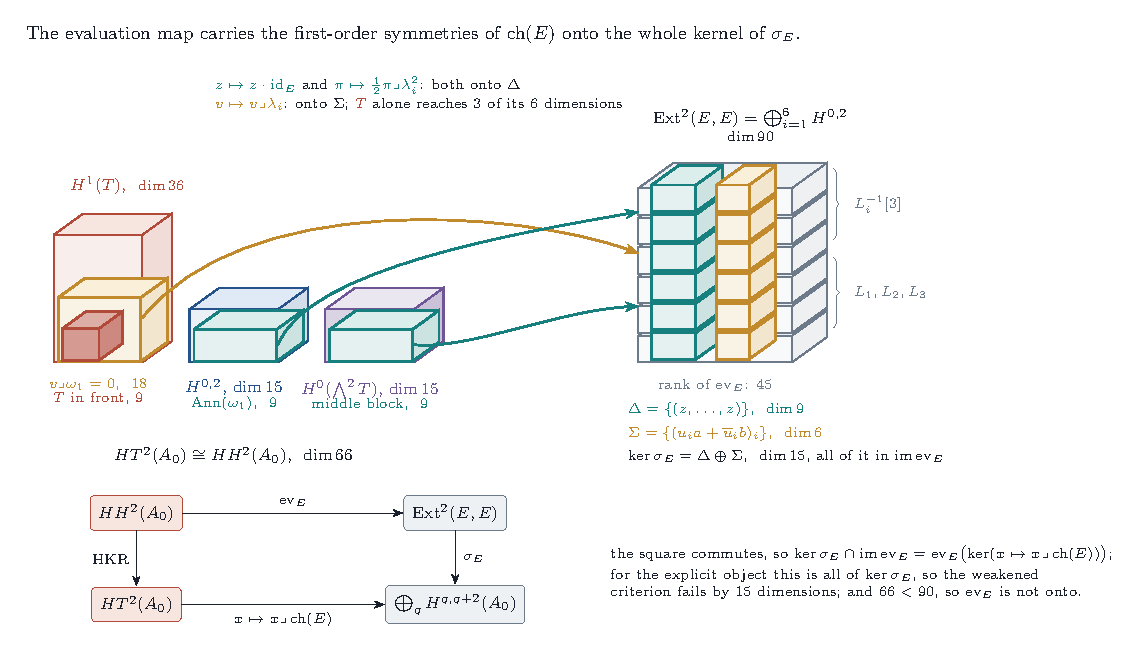
\includegraphics[width=\textwidth]{fig_evaluation}
\caption{\Cref{prop:evaluation} for the explicit object at $n=3$. Left: the
three summands of $HT^{2}(A_{0})$, drawn with heights proportional to their
dimensions, and inside each the part that preserves $\ch(E)$ to first order:
the annihilator of $\omega_{1}$, the deformations killing $\omega_{1}$ with
the polarised $K$-commuting tangent space $T$ in front, and the middle block
of bivectors. Right: $\Ext^{2}(E,E)$ as six stacked copies of $H^{0,2}$, one
per summand of $E$, and inside it the kernel of $\sigma_{E}$: the column
$\Delta$, one and the same class in every layer, and the column $\Sigma$,
whose entries depend on the summand through $u_{i}$. The three arrows are the
evaluation map on the three kernels; the two teal ones both land on
$\Delta$, the ochre one on $\Sigma$, and together they cover the kernel.
Below, the commutative square that makes this a statement about the weakened
criterion of \cite[Question 11.4]{Mar25b}.}
\label{fig:evaluation}
\end{figure}

\begin{remark}[Question 11.4 for split objects]
\label{rem:question114}
For a split object the two criteria stand or fall together, and for the
explicit object both fall completely. \Cref{thm:weakfails} makes the first
$n^{2}$ dimensions of the failure uniform over every concentrated object in
every dimension; \Cref{prop:evaluation}(iv) accounts for the remaining
$n(n-1)$ at $n=3$ by the deformations of the two halves $V_{\pm}$ of the
Hodge structure separately, and the equality $\ker\sigma_{E}=\Delta\oplus\Sigma$
says that the two mechanisms exhaust the kernel: nothing in it is
accidental. None of this touches the case for which the question was asked.
A sheaf of positive rank has $z\cdot\ch(E)\ne0$ for every $z\ne0$, so its
$\Delta$ is zero, and whether $\operatorname{ev}_{E}$ kills the deformations
that preserve $\kappa(E)$ is a statement about the sheaf and not about its
Chern character. Markman's candidate in \cite[Section 12]{Mar25b}, a rank
one complex on a principally polarised abelian fourfold with Chern character
on the secant $\langle e^{\pm\sqrt{-d}\Theta}\rangle$, is exactly such a
sheaf, and he records that the verification remains to be done.
\Cref{thm:factor} reduces that verification to one identity on the fourfold,
and \Cref{thm:candidatefails} shows that the identity fails: the candidate
does not satisfy the weakened criterion either.
\end{remark}

\subsubsection*{Solutions of nonzero rank}

We return to the Diophantine problem of \Cref{setup:pte}. By
\Cref{cor:nplusone} a solution with $\ch_{0}(E)\ne0$ needs at least $n+1$
distinct norms, and multiplicity one bounds each level sum by the number of
elements of $\cO_{K}$ of that norm.

\begin{proposition}[The level sums]\label{thm:pterange}
Keep \Cref{setup:pte} and suppose $E$ satisfies \eqref{eq:pteconditions} with
$\ch_{0}(E)\ne0$, so that the $u_{i}$ take $\nu\ge n+1$ distinct norms by
\Cref{cor:nplusone}. Write $N_{1}<\dots<N_{\nu}$ for those norms, $M_{j}$ for
the sum of the $m_{i}$ at level $N_{j}$, and
$r_{K}(N)=\#\{u\in\cO_{K}:\Nm_{K/\QQ}(u)=N\}$. If $\nu=n+1$ then, with
$P=\prod_{k}N_{k}$, $S=\ch_{0}(E)$ and
$D_{j}=N_{j}\prod_{k\ne j}(N_{j}-N_{k})$,
\begin{equation}\label{eq:levelsums}
  M_{j}=(-1)^{n}\,\frac{S\,P}{D_{j}},
\end{equation}
the least $S>0$ making every $M_{j}$ an integer is
$S_{\min}=\operatorname{lcm}_{j}\bigl(|D_{j}|/\gcd(|D_{j}|,P)\bigr)$, and
multiplicity one, \Cref{lem:splitsemireg}(i), forces
$|M_{j}|\le r_{K}(N_{j})$ for every $j$.
\end{proposition}

\begin{proof}
The conditions $T_{r,r}=0$ for $r=1,\dots,n$ say that the linear
functional $f\mapsto\sum_{j}M_{j}f(N_{j})$ kills $x,x^{2},\dots,x^{n}$, hence
sends every polynomial $f$ of degree at most $n$ to $S\,f(0)$. Applying it to
$f(x)=\prod_{k\ne j}(x-N_{k})$, which has degree $n$, gives
\[
  M_{j}\prod_{k\ne j}(N_{j}-N_{k})=S\,(-1)^{n}\prod_{k\ne j}N_{k},
\]
and multiplying by $N_{j}$ turns this into \eqref{eq:levelsums}. The value of
$S_{\min}$ is the definition of a least common multiple, and the bound on
$|M_{j}|$ holds because each $u$ of norm $N_{j}$ contributes at most one term
$m_{i}=\pm1$ to $M_{j}$.
\end{proof}

So the level sums are determined by the norms up to the scale $S$, and they
compete with the supply $r_{K}(N_{j})$ of elements at each level. That
competition is arithmetic. A second mechanism, in the cohomology of $A$,
closes the split route for every $n$ and every set of norms at once.

\begin{corollary}[Sums of line bundles fail both criteria]\label{cor:noline}
Let $A$ be of $(K,-1,n)$-Weil type with $n\ge2$, and let
$E=\bigoplus_{i}L_{i}[p_{i}]^{\oplus m_{i}}$ be a sum of shifted line bundles,
twisted by a common class or not, whose (twisted) Chern character remains of
Hodge type to first order along $\cD_{n,n}$ and has a nonzero Weil component.
Then $\sigma_{E}$ is not injective on the image of $\operatorname{ev}_{E}$:
$E$ is neither semiregular nor semiregular in the weakened sense of
\cite[Question 11.4]{Mar25b}, and it is obstructed to first order along some
direction of the Weil family. In particular every object of \Cref{setup:pte}
satisfying \eqref{eq:pteconditions}, for every $n\ge2$, every field $K$,
every rank and every set of norms, fails both criteria.
\end{corollary}

\begin{proof}
Write $\lambda_{i}$ for the twisted first Chern classes of the summands. If
every $\lambda_{i}$ were a real multiple of $\eta$, it would be a rational
multiple, both classes being rational, and the twisted Chern character
$\sum_{i}m_{i}e^{\lambda_{i}}$ would be a polynomial in $\eta$; its component
in degree $2n$ would then lie in $\QQ\eta^{n}$, which meets the Weil line in
zero by \Cref{prop:grading}, against the hypothesis. So some $\lambda_{i}$ is
not a real multiple of $\eta$, and \Cref{thm:linebundle} applies to the
summand $L_{i}[p_{i}]$. For an object of \Cref{setup:pte} the classes are
$\lambda_{i}=\theta(u_{i})\in R_{0}$, and $R_{0}\cap\QQ\eta=0$; no twist is
needed because $c_{1}(E)=\theta(T_{1,0})=0$ by \eqref{eq:pteconditions}, as
$(1,0)$ is not an excluded pair for $n\ge2$; and \eqref{eq:pteconditions}
gives a flat Chern character with a nonzero Weil component by
\Cref{prop:chintermsofu}.
\end{proof}

\begin{remark}[What the corollary asks of an object]\label{rem:nolinemeaning}
By \Cref{cor:noline} there is no sum of line bundles, at any member of any
Weil family in any dimension, that could run the semiregularity argument in
either form. The reason is \Cref{prop:rigidity}(i): the
only divisor class that stays of type $(1,1)$ across the whole family is the
polarisation, so every line bundle summand off that line is obstructed in
some direction of the family, and the semiregularity map, whose composite
with the obstruction is contraction with the flat class $\ch(E)$, cannot see
it. The object the argument needs is one with no rank one
summand off the polarisation line, of positive rank, indecomposable enough
that its Atiyah class contracted with every direction of $T$ vanishes.
Markman's reflexive sheaves at $n=3$ are of that kind, and nothing here
says that their analogues at $n\ge4$ do not exist.
\end{remark}

\subsection{Convolutions of line bundles}\label{ssec:convolutions}

After \Cref{cor:noline} the next objects built from line bundles are their
convolutions, the iterated cones of shifted line bundles. Their Chern
character is the same signed sum of exponentials as for a direct sum, but
their $\Ext$ groups are cut down by the maps between the pieces, so the
argument of \Cref{thm:linebundle} no longer applies as it stands. This
subsection shows that fewer than $2n$ pieces with nondegenerate differences
never serve (\Cref{thm:fewpieces}); writes down, at a CM member for
$K=\QQ(i)$, a signed sum of $2\cdot4^{n-1}$ line bundles that is exactly a
real Weil class (\Cref{prop:weilpieces}); and determines, for the
convolutions of those pieces with three multiples of the polarisation at
$n=3$, which products in the twisted differential can act on the $525$
diagonal classes of degree two, of which at least $468$ must disappear
before the polarised criterion can hold (\Cref{thm:esixdiagonal}). Nothing
enters the diagonal, cup products remove at most $276$ of these classes, and
everything else would have to be removed by fourfold products along a path
through the three multiples and one of the Weil pieces: one family of them
for some placements of the multiples, and two families that exclude each
other for the others (\Cref{prop:mixedplacement}); one order of the pieces
gives a convolution that solves the Maurer--Cartan equation
(\Cref{prop:explicitconvolution}). Off the diagonal, the classes between two
pieces that differ in every coordinate are reached by no product
(\Cref{lem:allthree}), and no
convolution of these pieces meets the polarised criterion
(\Cref{thm:noconvolution}). At $n=4$ the same classes, now between pieces
that differ in three coordinates, are reached by no product in any
convolution, and they exclude every convolution whose $128$ pieces
$L_{\zeta}$ occupy two shifts (\Cref{thm:efourtwolevels}) or three
consecutive ones (\Cref{thm:efourthreelevels}); with the groups between
pieces whose shifts differ by two or three (\Cref{lem:efourspread}) they
exclude every convolution whose pieces have their shifts within five
consecutive values (\Cref{cor:efourfive}); the diagonal classes at a lonely
shift (\Cref{lem:efourlonely}) and the interleaved shifts
(\Cref{prop:efourpairs}) extend this to six (\Cref{cor:efoursix}).

\begin{setupenv}[Convolutions]\label{setup:convolution}
Let $A$ be an abelian variety of dimension $g$ with a flat K\"ahler metric,
and let $L_{1},\dots,L_{m}$ be line bundles on $A$ with hermitian metrics of
constant curvature, hermitian forms $H_{1},\dots,H_{m}$ and pairwise distinct
first Chern classes. For integers $d_{1},\dots,d_{m}$ put
$P_{a}=L_{a}[-d_{a}]$. A \emph{convolution} of $P_{1},\dots,P_{m}$ is an
object $E$ given by a one-sided twisted
complex\footnote{Every object obtained from $P_{1},\dots,P_{m}$ by iterated
cones in this order is of this form, because the Dolbeault complexes form a
differential graded enhancement of the full subcategory of line bundles. All
the objects of this subsection are given in this way.}
\[
  \Bigl(\,\bigoplus_{a}\cA^{0,*}(L_{a})[-d_{a}],\ \bar\partial+\delta\Bigr),
  \qquad
  \delta=(\delta_{ab})_{a<b},\quad
  \delta_{ab}\in\cA^{0,1+d_{a}-d_{b}}\bigl(L_{a}^{-1}\otimes L_{b}\bigr),
\]
with $\bar\partial\delta+\delta\circ\delta=0$, so that
$\ch(E)=\sum_{a}(-1)^{d_{a}}e^{c_{1}(L_{a})}$. Write
$\cA(a,b)=\cA^{0,*}(L_{a}^{-1}\otimes L_{b})$ and $\cH(a,b)$ for its harmonic
forms, so that $\cH^{q}(a,b)\cong H^{q}(A,L_{a}^{-1}\otimes L_{b})$, and write
$\pi$, $G$ and $h=\bar\partial^{*}G$ for the harmonic projection, the Green
operator and the homotopy, with $1-\pi=\bar\partial h+h\bar\partial$ and
$\pi h=h\pi=h^{2}=0$. A form of degree $q$ in $\cA(a,b)$ is a morphism
$P_{a}\to P_{b}$ of degree $w=q-d_{a}+d_{b}$; we call $q$ its $\Ext$ degree
and, when $w=1$, call $q-1$ its \emph{excess}. When $H_{b}-H_{a}$ is
nondegenerate, $\cH(a,b)$ is concentrated in the single degree
$n(H_{b}-H_{a})$, the number of negative eigenvalues \cite[Chapter~3]{BL04}.
\end{setupenv}

\begin{lemma}[The harmonic model]\label{lem:harmonicmodel}
In \Cref{setup:convolution}:
\begin{enumerate}[label=\textup{(\roman*)},leftmargin=2.6em,itemsep=2pt]
\item $E$ is isomorphic to a convolution of the same pieces with
  $h\delta=0$, and then $\delta=\delta^{H}-h(\delta\circ\delta)$ with
  $\delta^{H}=\pi\delta$ harmonic. Substituting repeatedly, every
  $\delta_{ab}$ is a finite sum of planar binary trees whose leaves are
  components $\delta^{H}_{cd}$ with $c<d$, whose internal vertices compose,
  and whose internal edges carry $-h$.
\item $\Ext^{*}(E,E)$ is the cohomology of
  $\cH_{E}=\bigoplus_{a,b}\cH(a,b)$, graded by $w$, with the differential
  $d_{E}=\sum_{k\ge0}\pi\,Q(-hQ)^{k}$, where $Q=[\delta,-]$.
\item For $x\in\cH(a,b)$, the component of $d_{E}(x)$ in $\cH(c,e)$ is a sum
  of terms $\pm\pi\,T$, one for each planar binary tree $T$ with $k\ge2$
  leaves, internal vertices composing, $-h$ on the internal edges other
  than the root, whose leaves read in order are the components along a path
  $c=a_{0}\to a_{1}\to\dots\to a_{k}=e$ in which one step is
  $x\colon a\to b$ and the others are components $\delta^{H}_{a_{j}a_{j+1}}$
  with $a_{j}<a_{j+1}$. The $\Ext$ degree of such a term is the sum of the
  $\Ext$ degrees of its leaves minus $k-2$.
\end{enumerate}
\end{lemma}

The terms with $k$ leaves in (iii) are the Massey products of length $k$ of
the pieces;\footnote{In the language of $A_{\infty}$-categories they are the
higher products $m_{k}$ of the minimal model of the line bundles, evaluated
on the Maurer--Cartan element $\delta^{H}$ of the twisted complex; for
$k=2$ they are cup products.} (iii) is all that is used of them below.

\begin{proof}
(i) Suppose $h\delta_{cd}=0$ for $d-c<r$. Conjugating by $1+g$, with $g$ of
degree $0$ supported at distance $r$, replaces $\delta_{ab}$ for $b-a=r$ by
$X_{ab}+\bar\partial g_{ab}$, where $X_{ab}$ depends only on $\delta$, and
leaves the components at smaller distance unchanged. With
$g_{ab}=-hX_{ab}$ the new component is $X_{ab}-\bar\partial hX_{ab}$, and
$h\bar\partial h=h(1-\pi-h\bar\partial)=h$ gives $h(X_{ab}-\bar\partial
hX_{ab})=0$. Induction on $r$ gives $h\delta=0$, and then
$\delta=\pi\delta+\bar\partial h\delta+h\bar\partial\delta
=\delta^{H}-h(\delta\circ\delta)$ by the Maurer--Cartan equation. The
component $(\delta\circ\delta)_{ab}$ involves only components at distance
less than $b-a$, so the substitution ends.
(ii) The endomorphism complex of $E$ is $\bigoplus_{a,b}\cA(a,b)$ with the
differential $\bar\partial+Q$. Blockwise, the inclusion of harmonic forms,
$\pi$ and $-h$ form a strong deformation retraction of
$(\bigoplus\cA(a,b),\bar\partial)$ onto $(\cH_{E},0)$, and $Q$ raises $b-a$,
so $hQ$ is nilpotent. The basic perturbation lemma gives a homotopy
equivalence of $(\bigoplus\cA(a,b),\bar\partial+Q)$ with $(\cH_{E},d_{E})$,
with the chain maps $\iota_{E}=\sum_{k}(-hQ)^{k}$ on $\cH_{E}$ and
$\pi_{E}=\pi\sum_{k}(-Qh)^{k}$. (iii) Each $Q$ in $d_{E}$ composes with one
component of $\delta$ on the left or on the right; writing that component as
in (i) gives the trees, the edges from (i) and those from $d_{E}$ being
exactly the internal edges other than the root. Composition adds degrees,
$h$ lowers them by one, and a binary tree with $k$ leaves has $k-2$ internal
edges.
\end{proof}

\begin{lemma}[The index of a sum]\label{lem:indexsum}
For hermitian forms $X,Y$ on $\CC^{g}$, $n(X+Y)\le n(X)+n(Y)$. If
$H_{1}+\dots+H_{k}=0$, then $\sum_{j}n(H_{j})\ge g-\dim\ker H_{i}$ for every
$i$; in particular $\sum_{j}n(H_{j})\ge g$ when one $H_{i}$ is
nondegenerate.
\end{lemma}

\begin{proof}
A subspace on which $X+Y$ is negative definite meets the subspaces on which
$X\ge0$ and $Y\ge0$, of codimensions $n(X)$ and $n(Y)$, only in zero, so its
dimension is at most $n(X)+n(Y)$. For the second statement,
$-H_{i}=\sum_{j\ne i}H_{j}$ gives
$g-n(H_{i})-\dim\ker H_{i}=n(-H_{i})\le\sum_{j\ne i}n(H_{j})$.
\end{proof}

\begin{theorem}[Fewer than $2n$ pieces]\label{thm:fewpieces}
Let $A$ be of $(K,-1,n)$-Weil type with $n\ge2$, and let $E$ be a
convolution of $m<2n$ shifted line bundles whose differences $H_{b}-H_{a}$
are all nondegenerate. Suppose that $\ch(E)$ remains of Hodge type to first
order along $\cD_{n,n}$ and has a nonzero Weil component, as every polarised
character $N\omega_{1}+p(\theta)$ with $N\ne0$ does. Then there is
$v\in T_{[A]}\cD_{n,n}$ with
\[
  \operatorname{ev}_{E}(v)\ne0
  \qquad\text{and}\qquad
  \sigma_{E}\bigl(\operatorname{ev}_{E}(v)\bigr)=0 ,
\]
so $\sigma_{E}$ is not injective, and for a polarised character
$\dim\Ext^{2}(E,E)>r(\ch E)$ by \Cref{thm:p2primenumber}(iv).
\end{theorem}

\begin{proof}
First, no element of degree one of $\cH_{E}$ has a differential with a
nonzero component in the diagonal classes $\cH^{2}(c,c)=H^{2}(A,\cO_{A})$.
Such a component is a sum of terms of \Cref{lem:harmonicmodel}(iii) whose
$k$ leaves have degree one and run around a closed path $c\to\dots\to c$; the
pieces before the step $x$ increase from $c$ and those after it increase to
$c$, so the path passes through $k$ distinct pieces and $k\le m$. Its
leaves have $\Ext$ degrees $q_{j}=n(H_{a_{j+1}}-H_{a_{j}})$, and the output
has $\Ext$ degree $\sum_{j}q_{j}-(k-2)=2$, so $\sum_{j}q_{j}=k<2n$. The $k$
differences are nondegenerate and add up to zero, so \Cref{lem:indexsum}
gives $\sum_{j}q_{j}\ge g=2n$, a contradiction. Hence taking diagonal
components gives a well defined map
$\pi_{D}\colon\Ext^{2}(E,E)\to\bigoplus_{a}H^{2}(A,\cO_{A})$.

Next, $\operatorname{ev}_{E}(v)=v\lrcorner\mathrm{At}(E)$, as in the proof
of \Cref{thm:linebundle}. In the twisted complex the Atiyah class is
represented by the commutator of the Chern $(1,0)$-connection
$\bigoplus_{a}\nabla_{a}$ with $\bar\partial+\delta$; its diagonal entries
are the curvatures $F_{a}$, constant forms representing $c_{1}(L_{a})$, and
its other entries $\nabla\delta_{ab}$ lie above the diagonal. So
$\operatorname{ev}_{E}(v)$ is represented by an upper triangular $z$ with
$z_{aa}=v\lrcorner F_{a}$, and in $\cH_{E}$ by $\pi_{E}(z)$. The operators
$Q$ and $h$ preserve upper triangular forms and $Q$ makes them strictly upper
triangular, so the diagonal of $\pi_{E}(z)$ is that of $\pi(z)$, and
$\pi_{D}(\operatorname{ev}_{E}(v))=(v\lrcorner c_{1}(L_{a}))_{a}$.

If every $c_{1}(L_{a})$ were a real multiple of the polarisation, it would
be a rational one and $\ch(E)$ a polynomial in it, whose component in degree
$2n$ meets the Weil line in zero by \Cref{prop:grading}. So some
$c_{1}(L_{a})$ is not, and by \Cref{prop:rigidity}(i) some
$v\in T_{[A]}\cD_{n,n}$ has $v\lrcorner c_{1}(L_{a})\ne0$; then
$\pi_{D}(\operatorname{ev}_{E}(v))\ne0$, while
$\sigma_{E}(\operatorname{ev}_{E}(v))=v\lrcorner\ch(E)=0$.
\end{proof}

\Cref{thm:linebundle} is the case $\delta=0$, with any number of pieces. A
convolution reaches its diagonal classes once it has $2n$ pieces, when a
cycle through all of them can have total index $2n$, the equality case of
\Cref{lem:indexsum}. A convolution meeting the polarised criterion must
therefore have at least $2n$ pieces, or pieces with degenerate differences.
The next construction has both.

\begin{proposition}[A pure Weil class from line bundles]
\label{prop:weilpieces}
Let $E_{0}=\CC/\ZZ[i]$, $A=E_{0}^{2n}$ with coordinates $z_{1},\dots,z_{2n}$
and $n\ge2$, let $K=\QQ(i)$ act by $i$ on $z_{1},\dots,z_{n}$ and by $-i$
on $z_{n+1},\dots,z_{2n}$, and let $\theta$ be the product principal
polarisation; then $A$ is of $(\QQ(i),-1,n)$-Weil type, a CM member as in
\Cref{rem:cmquadratic}. Write $B_{j}$ for the surface with coordinates
$(z_{j},z_{n+j})$, so that $A=B_{1}\times\dots\times B_{n}$. For $p\in\ZZ$
and $\zeta\in\mu_{4}^{n}$ let $L_{\zeta}$ be a line bundle whose hermitian
form is $\bigl(\begin{smallmatrix}p&\zeta_{j}\\ \bbar\zeta_{j}&p
\end{smallmatrix}\bigr)$ on $B_{j}$ and zero between different surfaces, and
put $\alpha=\prod_{j}\tfrac{i}{2}\,dz_{j}\wedge d\bar z_{n+j}$.
\begin{enumerate}[label=\textup{(\roman*)},leftmargin=2.6em,itemsep=2pt]
\item $\alpha$ and $\bbar\alpha$ span the Weil classes of $A$, and
  \[
    \sum_{\prod\zeta=1}e^{c_{1}(L_{\zeta})}
    -\sum_{\prod\zeta=-1}e^{c_{1}(L_{\zeta})}
    =2\cdot4^{n-1}\,(\alpha+\bbar\alpha).
  \]
\item For distinct integers $t_{1},t_{2},t_{3}$ and signs $\sigma_{i}$, the
  character
  $\gamma=2\cdot4^{n-1}(\alpha+\bbar\alpha)+\sum_{i}\sigma_{i}e^{t_{i}\theta}$
  has Hankel rank $3$, so $r(\gamma)=7n^{2}-2n$. A convolution with this
  character of the $2\cdot4^{n-1}$ bundles $L_{\zeta}$, with
  $(-1)^{d}=\prod\zeta$, and of three line bundles $M_{i}$ with
  $c_{1}(M_{i})=t_{i}\theta$ has $2\cdot4^{n-1}+3$ pieces and
  $(2\cdot4^{n-1}+3)\,n(2n-1)$ diagonal classes of degree two: $525$
  against $r=57$ at $n=3$, and $3668$ against $104$ at
  $n=4$.\footnote{At $n=2$ the same construction has $8+3=11$ pieces and
  $66$ diagonal classes against $r=24$.}
\end{enumerate}
\end{proposition}

\begin{proof}
The hermitian forms have imaginary parts integral on $\ZZ[i]^{2n}$, so the
line bundles exist. On $B_{j}$ write $c_{1}$ of the restriction as
$p(a_{j}+b_{j})+\zeta_{j}c_{j}+\bbar\zeta_{j}c'_{j}$, where
$a_{j}=\tfrac i2dz_{j}\wedge d\bar z_{j}$,
$b_{j}=\tfrac i2dz_{n+j}\wedge d\bar z_{n+j}$,
$c_{j}=\tfrac i2dz_{j}\wedge d\bar z_{n+j}$ and
$c'_{j}=\tfrac i2dz_{n+j}\wedge d\bar z_{j}$. Since $c_{j}^{2}=c_{j}'^{2}=0$,
\[
  e^{c_{1}(L_{\zeta})}=\prod_{j}f_{j}(\zeta_{j}),\qquad
  f_{j}(z)=e^{p(a_{j}+b_{j})}\bigl(1+zc_{j}+\bbar zc'_{j}+c_{j}c'_{j}\bigr).
\]
For
$u\in\mu_{4}$, $\tfrac12(u+\bbar u)$ is $u$ when $u=\pm1$ and $0$ when
$u=\pm i$, so the left side of (i) is
$\tfrac12\bigl(\prod_{j}\sum_{z}zf_{j}(z)+\prod_{j}\sum_{z}\bbar zf_{j}(z)\bigr)$.
Now $\sum_{z\in\mu_{4}}z=\sum z^{2}=0$ and $\sum|z|^{2}=4$, so
$\sum_{z}zf_{j}(z)=4e^{p(a_{j}+b_{j})}c'_{j}=4c'_{j}$, because $a_{j}c'_{j}$
and $b_{j}c'_{j}$ repeat a differential, and likewise
$\sum_{z}\bbar zf_{j}(z)=4c_{j}$. This gives
$2\cdot4^{n-1}(\prod c'_{j}+\prod c_{j})=2\cdot4^{n-1}(\bbar\alpha+\alpha)$.
The differentials $dz_{j}$, $j\le n$, and $d\bar z_{n+j}$ span the
$i$-eigenspace of $K$ on $H^{1}(A,\CC)$, and $\alpha$ spans its top exterior
power, which is a Weil class, and $\bbar\alpha$ the conjugate one. (ii) The
moments $\mu_{m}=\sum_{i}\sigma_{i}t_{i}^{m}$ make the Hankel matrix of
\Cref{setup:p2prime} a product of Vandermonde matrices of rank $3$, and
\Cref{thm:p2primenumber}(ii) gives $r$. The counts are immediate.
\end{proof}

The pieces $L_{\zeta}$ and $L_{\zeta'}$ have a degenerate difference as soon
as $\zeta$ and $\zeta'$ share a coordinate, so \Cref{thm:fewpieces} does not
apply to them, and there are more than $2n$ of them. The rest of this
subsection computes what the Massey products can do to the diagonal classes
of such a convolution. The pieces are external products over the surfaces
$B_{j}$, and the first tool is a bound on how far a product can lower the
degree on each surface.

\begin{lemma}[Degree drop on a product]\label{lem:degreedrop}
Let $A=B_{1}\times\dots\times B_{n}$ with a product metric, and let every
$L_{a}$ be an external product with a product metric. Decompose the leaves
of a term of \Cref{lem:harmonicmodel}(iii) with $k$ leaves into tensor
products of harmonic forms on the factors. Then the output has degree
$s_{j}-d_{j}$ on $B_{j}$, where $s_{j}$ is the sum of the degrees of the
leaves on $B_{j}$ and $d_{j}\ge0$, $\sum_{j}d_{j}=k-2$, and
\[
  d_{j}\le\max(0,\,u_{j}-2),
\]
where $u_{j}$ is the number of leaves whose component on $B_{j}$ is not a
multiple of the unit section of $\cO_{B_{j}}$ (such a unit occurs only where
source and target agree on $B_{j}$).
\end{lemma}

\begin{proof}
The Laplacian is $\Delta=\sum_{j}\Delta_{j}$, so $h=\sum_{j}h_{j}$ with
$h_{j}=\bar\partial_{j}^{*}G=G\bar\partial_{j}^{*}$, which lowers the degree
on $B_{j}$ by one and keeps the others; expand every internal edge
accordingly, and let $d_{j}$ be the number of edges carrying $h_{j}$. Let
$V_{j}$, $U_{j}$ and $W_{j}$ be the forms whose component on $B_{j}$ is
$\Delta_{j}$-harmonic, a multiple of the unit, or in the image of
$\bar\partial_{j}^{*}$. The operators $G$ and $h_{i}$, $i\ne j$, preserve all
three, $h_{j}$ kills $V_{j}$ and $W_{j}$, $\pi$ kills $W_{j}$, and
multiplication by an element of $U_{j}$ preserves $V_{j}$, $U_{j}$ and
$W_{j}$. For an edge $e$ carrying $h_{j}$ let $N(e)$ be the set of leaves
below $e$ whose component on $B_{j}$ is not a unit. If $|N(e)|\le1$ the
value below $e$ lies in $V_{j}$ and the term vanishes. If $e$ lies below the
next such edge $e'$ with $N(e)=N(e')$, everything composed in between lies
in $U_{j}$, the value at $e'$ lies in $W_{j}$, and the term vanishes; if
$N(e)$ is the set of all $u_{j}$ such leaves for the highest such edge, the
value at the root lies in $W_{j}$ and $\pi$ kills it. So in a nonzero term
the sets $N(e)$ are distinct, of size at least two, different from the whole
set, and pairwise nested or disjoint. Together with the whole set they form
a family of that kind, which has at most $u_{j}-1$ members, since its members
are the internal vertices of a forest with $u_{j}$ leaves in which every
internal vertex has at least two children. Hence $d_{j}\le u_{j}-2$.
\end{proof}

\begin{proposition}[Nothing enters the diagonal]\label{prop:nothingenters}
Keep \Cref{prop:weilpieces} with $n\ge3$, and let $t_{1},t_{2},t_{3}$ be
distinct with $|t_{i}-p|\ge2$. For every convolution $E$ of the pieces
$L_{\zeta}$ and $M_{i}$, in any order, with any shifts of the given parities
and with the pieces twisted by any line bundles of degree zero, no element of
degree one of $\cH_{E}$ has a differential with a nonzero diagonal
component. Consequently
\[
  \dim\Ext^{2}(E,E)\;\ge\;\dim\ker\bigl(d_{E}|_{D^{2}}\bigr),
  \qquad
  D^{2}=\bigoplus_{a}H^{2}(A,\cO_{A}).
\]
\end{proposition}

\begin{proof}
As in the proof of \Cref{thm:fewpieces}, a term that reaches the diagonal
runs around a closed path of distinct pieces whose $k$ steps have degree one
and total excess $0$. The step from $L_{\zeta}$ to $L_{\zeta'}$ has $\Ext$
degree $1$ on each surface where $\zeta_{j}\ne\zeta'_{j}$, the difference
there having eigenvalues $\pm|\zeta'_{j}-\zeta_{j}|$, and at least $0$
elsewhere. If $\prod\zeta=\prod\zeta'$ the two differ on at least two
surfaces; otherwise the step has even $\Ext$ degree, the shifts having
opposite parities. Either way its excess is at least $1$. The difference
between $L_{\zeta}$ and $M_{i}$ has eigenvalues $t_{i}-p\pm1$ on every
surface, so it is definite: the step has $\Ext$ degree $0$ and excess $-1$
if it goes up the value $\phi$, where $\phi(L_{\zeta})=p$ and
$\phi(M_{i})=t_{i}$, and $\Ext$ degree $2n$ and excess $2n-1$ if it goes
down; the same holds between the $M_{i}$. A maximal run of the cycle through
the $M_{i}$ starts and ends at the value $p$, or is the whole cycle, so it
has at least one step down and at most three steps up; its excess is at least
$2n-1-3\ge2$. So every cycle has excess at least $1$. Twisting by line
bundles of degree zero leaves the forms unchanged and can only make some
$\cH(a,b)$ vanish. For the inequality, the diagonal components of cocycles
of degree two vanish on coboundaries, so $\dim\Ext^{2}(E,E)$ is at least the
dimension of their image, which contains the kernel of $d_{E}$ on $D^{2}$.
\end{proof}

At $n=2$ the bound on a run is $0$ and a cycle through the three multiples
can reach the diagonal; this is why the analysis below starts at $n=3$.

\begin{figure}[tbp]
\centering
  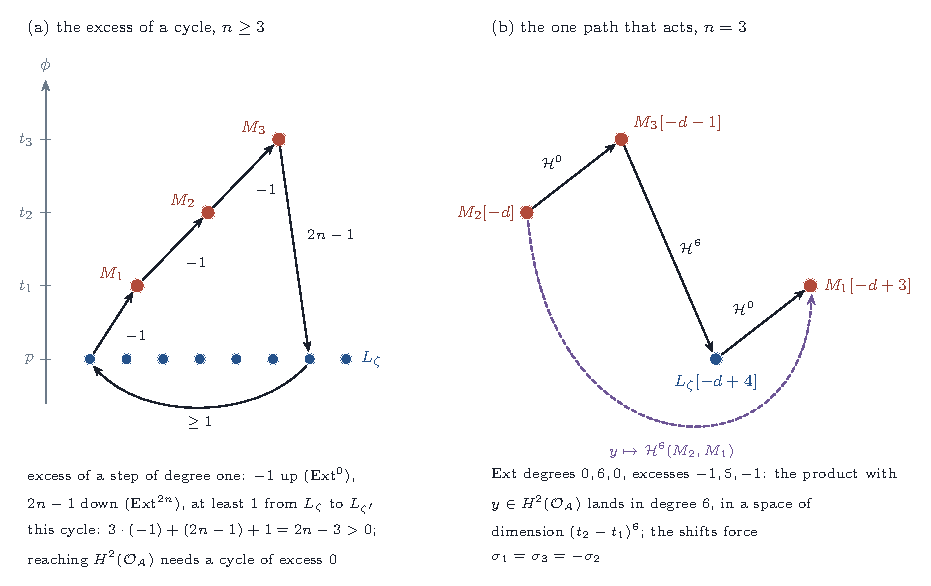
\includegraphics[width=\textwidth]{fig_convolutions}
\caption{The pieces of \Cref{prop:weilpieces} at their values $\phi$, with
$\phi(L_{\zeta})=p$ and $\phi(M_{i})=t_{i}$. (a) A step of degree one
between pieces with a definite difference has $\Ext$ degree $0$ going up
and $2n$ going down, so excess $-1$ or $2n-1$; a step between two
$L_{\zeta}$ has excess at least $1$. The cycle drawn runs up through all
three $M_{i}$ and down once, the worst case, and still has excess
$2n-3>0$, so for $n\ge3$ no term reaches the diagonal
(\Cref{prop:nothingenters}). (b) The one path whose products act on the
diagonal at $n=3$ when the $t_{i}$ lie above $p$
(\Cref{thm:esixdiagonal}(i)), drawn at the same heights
and in the order of the convolution, with the $\Ext$ degrees of its steps
and the shifts they force; the dashed arrow is the value of the product with
a diagonal class $y$.}
\label{fig:convolutions}
\end{figure}

\begin{proposition}[Cup products on the diagonal]\label{prop:cupkernel}
Keep \Cref{prop:nothingenters} with $n=3$, so that $D^{2}$ has dimension
$35\cdot15=525$. The terms of $d_{E}$ on $D^{2}$ with two leaves, the cup
products, vanish on the $45$ diagonal classes of the $M_{i}$, and on the
$480$ diagonal classes of the $L_{\zeta}$ they have a kernel of dimension at
least $204$. So their kernel on $D^{2}$ has dimension at least $249$.
\end{proposition}

\begin{proof}
For $y=(y_{a})\in D^{2}$ the cup products in $\cH(a,b)$ are
$(y_{a}-y_{b})\wedge\delta^{H}_{ab}$, since $y$ has even degree. On a surface
where the pieces differ, $\delta^{H}_{ab}$ has degree $1$, the only degree of
the cohomology there, and the product with a component of $y$ of positive
degree lands in a degree where the cohomology vanishes. The pieces $M_{i}$
differ from every other piece on every surface, which gives the first
statement. Write $y_{a}$ by its type $\tau\in\{0,1,2\}^{3}$, $|\tau|=2$, the
degrees on the three surfaces: three types $(2,0,0)$ of dimension one and
three types $(1,1,0)$ of dimension four. The degree count on each surface
and the parity of $\Ext$ degrees show that $L_{\zeta}$ and $L_{\zeta'}$ can
carry a nonzero cup product on the type $\tau$ only if either $\zeta'$
differs from $\zeta$ by a sign in one coordinate outside the support of
$\tau$, or $\zeta'$ is $\zeta$ multiplied by $(i,i)$ or $(-i,-i)$ in two
coordinates and $\tau$ is $2$ on the third. Let $\Gamma_{\tau}$ be the graph
on the $32$ pieces with these edges. If each component $y^{\tau}$ is
constant on the connected components of $\Gamma_{\tau}$, every cup product
vanishes. For $\tau=(2,0,0)$ the coordinate $\zeta_{1}$ is constant along
the edges, and the eight pieces with a given $\zeta_{1}$ are connected, so
$\Gamma_{\tau}$ has $4$ components; for $\tau=(1,1,0)$ the edges change the
sign of $\zeta_{3}$ only, and $\Gamma_{\tau}$ has $16$ components. The
kernel therefore contains a space of dimension $3\cdot4\cdot1+3\cdot16\cdot4
=12+192=204$.
\end{proof}

\begin{theorem}[The diagonal on $E_{0}^{6}$]\label{thm:esixdiagonal}
Let $n=3$ and let $E$ be a convolution of the $32$ bundles $L_{\zeta}$ and
of $M_{1},M_{2},M_{3}$ as in \Cref{prop:weilpieces}, with
$p+2\le t_{1}<t_{2}<t_{3}$ and signs $\sigma_{i}$, so that
$\ch(E)=32(\alpha+\bbar\alpha)+\sum_{i}\sigma_{i}e^{t_{i}\theta}$ and the
polarised criterion asks for $\dim\Ext^{2}(E,E)=57$.
\begin{enumerate}[label=\textup{(\roman*)},leftmargin=2.6em,itemsep=2pt]
\item The Massey products of length at least three vanish on $D^{2}$, except
  those of length four along a path
  $M_{2}\to M_{3}\to L_{\zeta}\to M_{1}$ taken in this order in the
  convolution, which occur only if $\sigma_{1}=\sigma_{3}=-\sigma_{2}$ and
  take values in
  $\cH^{6}(M_{2},M_{1})\cong H^{6}\bigl(A,\cO_{A}(-(t_{2}-t_{1})\theta)\bigr)$,
  of dimension $(t_{2}-t_{1})^{6}$.
\item $\dim\Ext^{2}(E,E)\ge249-\min\bigl(249,(t_{2}-t_{1})^{6}\bigr)$, and
  $\dim\Ext^{2}(E,E)\ge249$ unless the order and the signs are as in (i).
  In particular $E$ does not meet the polarised criterion when
  $t_{2}-t_{1}\le2$, since $249-64=185>57$, nor when the signs or the order
  differ from (i).
\item If $E$ meets the polarised criterion, then the length four products
  of (i) have rank at least $249-57=192$ on the kernel of the cup products,
  and $t_{2}-t_{1}\ge3$.
\end{enumerate}
The same holds for $t_{1}<t_{2}<t_{3}\le p-2$ with $E$ replaced by its dual.
\end{theorem}

\begin{proof}
(i) By \Cref{lem:harmonicmodel}(iii) a term with $k\ge3$ leaves acting on
$y\in H^{2}(\cO_{A})$ at a piece $c$ runs along a chain
$s=a_{0}\to\dots\to a_{k-1}=e$ of distinct pieces, increasing in the order
of the convolution, whose $k-1$ steps are components of degree one, with $y$
inserted at $c$. Its value lies in $\cH(s,e)$, in $\Ext$ degree
$2+\sum_{j}q_{j}-(k-2)=3+\varepsilon$, where $\varepsilon$ is the sum of the
excesses of the steps; so $-3\le\varepsilon\le3$, and $\cH(s,e)$ must be
nonzero in degree $3+\varepsilon$. By the proof of \Cref{prop:nothingenters}
a step between two $L_{\zeta}$ has excess at least $1$, with equality only
between pieces of opposite parities, and a step between pieces at different
values of $\phi$ has excess $-1$ and $\Ext$ degree $0$ going up, excess $5$
and $\Ext$ degree $6$ going down. Let $U$ and $D$ be the numbers of steps
up and down and $\lambda$ the total excess of the steps between two
$L_{\zeta}$, so that $\varepsilon=5D-U+\lambda$. For two distinct
$L_{\zeta}$, $L_{\zeta'}$ differing in $m\ge1$ coordinates, $\cH(L_{\zeta},
L_{\zeta'})$ vanishes above degree $6-m$; for pieces at different values it
sits in degree $0$ if the target is higher and in degree $6$ if it is lower.

Two observations remove chains. First, a chain of total excess $-2$ has no
step down, and so consists of steps between $L_{\zeta}$ followed by at most
three steps up. Second, let $a\to b\to c$ be two consecutive steps of
$\Ext$ degree $0$, sections $x_{ab}$ and $x_{bc}$ of line bundles. The
Maurer--Cartan equation $\pi(\delta\circ\delta)=0$ of the proof of
\Cref{prop:explicitconvolution}(i) has, in $\cH^{0}(a,c)$, one term for each
chain from $a$ to $c$ of total excess $-2$. If $a\to b\to c$ is the only such
chain, the equation reads $x_{ab}x_{bc}=0$, a product of holomorphic
sections being holomorphic and so harmonic; since $A$ is connected, $x_{ab}$
or $x_{bc}$ vanishes, and every term along a chain through both steps is
zero.

Here every step up ends at one of $M_{1},M_{2},M_{3}$, so $U\le3$, and
$D\le1$. If $D=0$, the chain is $r\ge0$ pieces $L_{\zeta}$ followed by
multiples in increasing order. When it ends at an $L_{\zeta}$, $k\ge3$ gives
$\lambda\ge2$, so $s$ and $e$ differ in one coordinate and $\lambda=2$; then
the two steps change the parity twice, whereas $s$ and $e$ have opposite
parities. When it ends at a multiple, $e$ lies above $s$, so $\varepsilon=-3$,
which forces $U=3$, $\lambda=0$ and the chain $L_{\zeta}\to M_{1}\to
M_{2}\to M_{3}$; by the first observation $L_{\zeta}\to M_{1}\to M_{2}$ is the
only chain of excess $-2$ from $L_{\zeta}$ to $M_{2}$, and the second removes
it. If $D=1$, then $U\ge2+\lambda$, so $(U,\lambda)$ is $(2,0)$, $(3,0)$ or
$(3,1)$ and $\varepsilon$ is $3$, $2$ or $3$. For $\varepsilon=3$ the piece
$s$ is a multiple and $e$ lies below it. With $(3,1)$ the three steps up
would end at three multiples other than $s$, which do not exist. With $(2,0)$
the chain has three steps, and a step down lands at an $L_{\zeta}$, since a
fourth multiple does not exist. It is $M_{1}\to M_{2}\to M_{3}\to L_{\zeta}$,
removed by the second observation at $M_{1}\to M_{2}\to M_{3}$; or
$M_{a}\to M_{b}\to L_{\zeta}\to M_{c}$ with $t_{a}<t_{b}$ and $t_{c}<t_{a}$,
that is $M_{2}\to M_{3}\to L_{\zeta}\to M_{1}$; or
$M_{a}\to L_{\zeta}\to M_{b}\to M_{c}$ with $t_{b}<t_{c}<t_{a}$, that is
$M_{3}\to L_{\zeta}\to M_{1}\to M_{2}$, removed at $L_{\zeta}\to M_{1}\to
M_{2}$. For $\varepsilon=2$, with $(U,\lambda)=(3,0)$, the pieces $s$ and $e$
are $L_{\zeta}$ differing in one coordinate; the last step is the step down,
preceded by three steps up from $s$, so the chain is $L_{\zeta}\to M_{1}\to
M_{2}\to M_{3}\to L_{\zeta'}$, removed at $L_{\zeta}\to M_{1}\to M_{2}$.

Only $M_{2}\to M_{3}\to L_{\zeta}\to M_{1}$ remains. Its steps have $\Ext$
degrees $0$, $6$ and $0$, so degree one forces $d_{M_{3}}=d_{M_{2}}+1$,
$d_{L}=d_{M_{3}}-5$ and $d_{M_{1}}=d_{L}+1$; this gives the signs, and the
value lies in
$\cH^{3+d_{M_{2}}-d_{M_{1}}}(M_{2},M_{1})=\cH^{6}(M_{2},M_{1})$, whose
dimension is $|\chi(\cO_{A}((t_{1}-t_{2})\theta))|=(t_{2}-t_{1})^{6}$.
(ii) By \Cref{prop:nothingenters} it suffices to bound the kernel of $d_{E}$
on $D^{2}$. By \Cref{prop:cupkernel} the cup products have a kernel $Y$ of
dimension at least $249$, and on $Y$ the differential is the sum of the
products of (i), of rank at most $(t_{2}-t_{1})^{6}$. (iii) follows from
(ii). For the dual, $E\mapsto E^{\vee}$ preserves $\Ext^{2}$ and sends the
configuration with $p$, $t_{i}$ to the one with $-p$, $-t_{i}$, the set of
the $L_{\zeta}$ being stable under $\zeta\mapsto-\zeta$.
\end{proof}

\begin{figure}[tbp]
\centering
  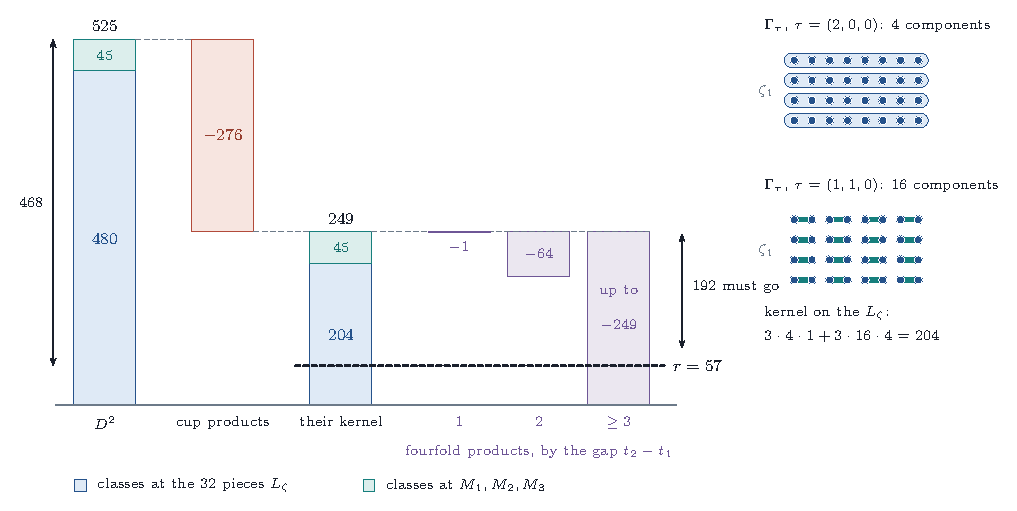
\includegraphics[width=\textwidth]{fig_diagonalbudget}
\caption{The $525$ diagonal classes of degree two at $n=3$
(\Cref{prop:cupkernel,thm:esixdiagonal}). The cup products remove $276$ of
them for general components, and at most that many in any case, leaving
$204$ at the pieces $L_{\zeta}$ and the $45$ at the $M_{i}$; when the $t_{i}$
lie on one side of $p$, the fourfold products of the surviving path remove
at most $(t_{2}-t_{1})^{6}$ more,
which is $1$ or $64$ for the gaps $1$ and $2$ and no constraint from the
third gap on. The criterion asks for $57$, so $468$ classes must disappear
in all and $192$ after the cup products. On the right, the graphs
$\Gamma_{\tau}$ on the $32$ pieces, one row for each value of $\zeta_{1}$:
for $\tau=(2,0,0)$ each row is a component, for $\tau=(1,1,0)$ the
components are the pairs differing in the sign of $\zeta_{3}$; a class
constant on the components of every $\Gamma_{\tau}$ has vanishing cup
products.}
\label{fig:diagonalbudget}
\end{figure}

The placements of the $t_{i}$ on both sides of $p$ are not covered by
\Cref{thm:esixdiagonal}. There two families of fourfold products occur
instead of one, and no convolution carries both.

\begin{proposition}[Placements on both sides of $p$]\label{prop:mixedplacement}
Keep \Cref{thm:esixdiagonal}, but let $t_{1}\le p-2$ and
$p+2\le t_{2}<t_{3}$.
\begin{enumerate}[label=\textup{(\roman*)},leftmargin=2.6em,itemsep=2pt]
\item The Massey products of length at least three vanish on $D^{2}$ unless
  $\sigma_{1}=\sigma_{2}=-\sigma_{3}$. In that case the only ones that act
  have length four and run along one of the paths
  \[
    \textup{(a)}\ \ M_{2}\to M_{3}\to M_{1}\to L_{\zeta},
    \qquad
    \textup{(b)}\ \ M_{3}\to M_{1}\to L_{\zeta}\to M_{2},
  \]
  taken in this order in the convolution, with $\prod\zeta=\sigma_{3}$. The
  products along (a) take values in $\cH^{6}(M_{2},L_{\zeta})$, of dimension
  $\bigl((t_{2}-p)^{2}-1\bigr)^{3}$, and those along (b) in
  $\cH^{6}(M_{3},M_{2})$, of dimension $(t_{3}-t_{2})^{6}$. A convolution
  carries at most one of the two kinds, since (a) puts $M_{2}$ before $M_{3}$
  and (b) puts $M_{3}$ before $M_{2}$.
\item If $E$ meets the polarised criterion, then
  $\sigma_{1}=\sigma_{2}=-\sigma_{3}$, and the products along (a) or those
  along (b) have rank at least $192$ on the kernel of the cup products. For
  (b) this needs $t_{3}-t_{2}\ge3$. The sixteen targets of (a) have
  dimension $16\bigl((t_{2}-p)^{2}-1\bigr)^{3}\ge432$, so for (a) the
  count gives no condition.
\end{enumerate}
For $t_{1}<t_{2}\le p-2$ and $t_{3}\ge p+2$ the same holds for
$E^{\vee}[1]$, and the condition on the signs becomes
$\sigma_{2}=\sigma_{3}=-\sigma_{1}$.
\end{proposition}

\begin{proof}
(i) We use the notation and the two observations of the proof of
\Cref{thm:esixdiagonal}(i). Now $\phi(M_{1})=t_{1}<p<t_{2}<t_{3}$; a step up
ends at $M_{2}$, at $M_{3}$, or at an $L_{\zeta}$ coming from $M_{1}$, so
again $U\le3$ and $D\le1$. If $D=0$, the values do not decrease along the
chain. When $e$ lies above $s$, $\varepsilon=-3$ forces $U=3$, $\lambda=0$
and the chain $M_{1}\to L_{\zeta}\to M_{2}\to M_{3}$, removed at
$L_{\zeta}\to M_{2}\to M_{3}$, the only chain of excess $-2$ from
$L_{\zeta}$ to $M_{3}$. When $e$ and $s$ have the same value, they are two
$L_{\zeta}$ joined by steps between $L_{\zeta}$, which is excluded as before.
If $D=1$, $(U,\lambda)$ is $(2,0)$, $(3,0)$ or $(3,1)$. For
$\varepsilon=3$, $e$ lies below $s$. With $(3,1)$ the steps up end at
$M_{2}$, $M_{3}$ and an $L_{\zeta}$ following $M_{1}$; then $s$ is an
$L_{\zeta}$, so $e=M_{1}$, which is followed by a step: impossible. With
$(2,0)$ the chain has three steps and no two consecutive $L_{\zeta}$. As
$M_{1}$ is the lowest piece, it is never the end of a step up, and a step up
into an $L_{\zeta}$ comes from $M_{1}$; so two consecutive steps up end at
$M_{2}$ or $M_{3}$. The chain cannot start at $M_{1}$. If it starts at an
$L_{\zeta}$, it ends at $M_{1}$ with the step down, after two steps up:
$L_{\zeta}\to M_{2}\to M_{3}\to M_{1}$, removed at $L_{\zeta}\to M_{2}\to
M_{3}$. If it starts at $M_{3}$, the first step goes down and the last two
go up, ending at $M_{2}$; the middle piece is then an $L_{\zeta}$ entered
from $M_{1}$, and the chain is $M_{3}\to M_{1}\to L_{\zeta}\to M_{2}$, path
(b). If it starts at $M_{2}$, then $e\in\{L_{\zeta},M_{1}\}$, so the last two
steps are not both up; the first step goes up to $M_{3}$, the second down,
and the third up into $e=L_{\zeta}$ from $M_{1}$: the chain is $M_{2}\to
M_{3}\to M_{1}\to L_{\zeta}$, path (a). For $\varepsilon=2$,
$(U,\lambda)=(3,0)$ and $s$, $e$ are $L_{\zeta}$ differing in one
coordinate. The last step enters $e$ from $M_{1}$, since a step down into
$e$ would follow three steps up from $s$, one more than the values allow;
$M_{1}$ is entered by the step down, after two steps up from $s$:
$L_{\zeta}\to M_{2}\to M_{3}\to M_{1}\to L_{\zeta'}$, removed at
$L_{\zeta}\to M_{2}\to M_{3}$.
Along (a) the steps have $\Ext$ degrees $0$, $6$ and $0$, so degree one
forces $d_{M_{3}}=d_{M_{2}}+1$, $d_{M_{1}}=d_{M_{3}}-5$ and
$d_{L}=d_{M_{1}}+1$. Along (b) they have $\Ext$ degrees $6$, $0$ and $0$,
which forces $d_{M_{1}}=d_{M_{3}}-5$, $d_{L}=d_{M_{1}}+1$ and
$d_{M_{2}}=d_{L}+1$. This gives the signs and puts the values in
$\cH^{3+d_{M_{2}}-d_{L}}(M_{2},L_{\zeta})=\cH^{6}(M_{2},L_{\zeta})$ and in
$\cH^{3+d_{M_{3}}-d_{M_{2}}}(M_{3},M_{2})=\cH^{6}(M_{3},M_{2})$. On $B_{j}$
the line bundle $L_{\zeta}\otimes M_{2}^{-1}$ has the hermitian form
$\bigl(\begin{smallmatrix}p-t_{2}&\zeta_{j}\\ \bbar\zeta_{j}&p-t_{2}
\end{smallmatrix}\bigr)$, with eigenvalues $p-t_{2}\pm1<0$ and determinant
$(t_{2}-p)^{2}-1$, which gives the first dimension. The second is that of
\Cref{thm:esixdiagonal}(i) with $t_{3}$, $t_{2}$ in place of $t_{2}$,
$t_{1}$.
(ii) \Cref{prop:nothingenters,prop:cupkernel} do not depend on the
placement of the $t_{i}$, so as in \Cref{thm:esixdiagonal}(ii)
$\dim\Ext^{2}(E,E)\ge249-\rho$, where $\rho$ is the rank on the kernel of
the cup products of the products of (i) that $E$ carries, and $\rho=0$
unless $\sigma_{1}=\sigma_{2}=-\sigma_{3}$. The criterion asks for $57$,
so $\rho\ge192$, and $(t_{3}-t_{2})^{6}\ge192$ exactly when
$t_{3}-t_{2}\ge3$. For the last statement, $E\mapsto E^{\vee}[1]$ preserves
$\Ext^{2}$, sends $p$ and the $t_{i}$ to $-p$ and the $-t_{i}$, reverses the
order of the pieces and changes every sign.
\end{proof}

The Maurer--Cartan equation can be solved for one order of the pieces.

\begin{proposition}[An explicit convolution]\label{prop:explicitconvolution}
Keep \Cref{thm:esixdiagonal} with $p=0$ and $t=(2,5,6)$, take the pieces to
be external products $L_{\zeta}=N_{1,\zeta_{1}}\boxtimes N_{2,\zeta_{2}}
\boxtimes N_{3,\zeta_{3}}$ and $M_{i}=M_{i,1}\boxtimes M_{i,2}\boxtimes
M_{i,3}$ of line bundles on the $B_{j}$, and order them as $M_{2}$, $M_{3}$,
the sixteen $L_{\zeta}$ with $\prod\zeta=1$, $M_{1}$, the sixteen $L_{\zeta}$
with $\prod\zeta=-1$, with the shifts $0$, $1$, $-4$, $-3$, $-5$.
\begin{enumerate}[label=\textup{(\roman*)},leftmargin=2.6em,itemsep=2pt]
\item The components that the degrees allow are
  $x_{1}\in\cH^{0}(M_{2},M_{3})$, $x_{2}^{\zeta}\in\cH^{6}(M_{3},L_{\zeta})$,
  $x_{3}^{\zeta}\in\cH^{0}(L_{\zeta},M_{1})$, components in
  $\cH^{2}(L_{\zeta},L_{\zeta'})$ for the $48+96$ pairs with
  $\prod\zeta=1=-\prod\zeta'$ that differ in one or two coordinates, and
  components in $\cH^{6}(M_{2},L_{\zeta'})$, $\prod\zeta'=-1$, which we take
  to be zero. For harmonic components the Maurer--Cartan equation is exactly
  \[
    x_{1}x_{2}^{\zeta}=0\ \text{in}\ H^{6}(A,M_{2}^{-1}\otimes L_{\zeta})
    \ \text{for every}\ \zeta,
    \qquad
    \sum_{\zeta}x_{2}^{\zeta}x_{3}^{\zeta}=0\ \text{in}\
    H^{6}(A,M_{3}^{-1}\otimes M_{1}),
  \]
  and every solution is the harmonic part of a convolution $E$ with
  $\ch(E)=32(\alpha+\bbar\alpha)+e^{5\theta}-e^{6\theta}-e^{2\theta}$.
\item There are solutions with every $x_{2}^{\zeta}\ne0$ and
  $x_{1}x_{2}^{\zeta}=x_{2}^{\zeta}x_{3}^{\zeta}=0$.
\item For every solution $\dim\Ext^{2}(E,E)\ge2560$, so $E$ does not meet
  the polarised criterion.
\end{enumerate}
\end{proposition}

\begin{proof}
(i) A component from $P_{a}$ to $P_{b}$ has $\Ext$ degree $1+d_{a}-d_{b}$, and
the forms give the cohomology of each pair: $\cH(M_{2},M_{3})$ and
$\cH(L_{\zeta},M_{1})$ sit in degree $0$, $\cH(M_{3},L_{\zeta})$,
$\cH(M_{2},L_{\zeta'})$ and $\cH(M_{2},M_{1})$ in degree $6$, and
$\cH(L_{\zeta},L_{\zeta'})$ in degree $2$ exactly for the pairs listed; no
other pair has cohomology in the degree a component needs. Put
$\delta=\delta^{H}-h(\delta\circ\delta)$ recursively, as in
\Cref{lem:harmonicmodel}(i), and $\Phi=\bar\partial\delta+\delta\circ\delta$.
Then $\Phi=\pi(\delta\circ\delta)+h\bar\partial(\delta\circ\delta)$ and
$\bar\partial(\delta\circ\delta)=\Phi\circ\delta-\delta\circ\Phi$, so by
induction on $b-a$ the twisted complex exists exactly when
$\pi(\delta\circ\delta)=0$. The components of $\pi(\delta\circ\delta)$ come
from paths of two or more components; those that land in a nonzero group
are $x_{1}x_{2}^{\zeta}$ in $\cH^{6}(M_{2},L_{\zeta})$ and
$\sum_{\zeta}x_{2}^{\zeta}x_{3}^{\zeta}$ in $\cH^{6}(M_{3},M_{1})$, while the
product along $M_{2}\to M_{3}\to L_{\zeta}\to M_{1}$ would lie in
$\cH^{5}(M_{2},M_{1})=0$ and $x_{2}^{\zeta}$ composed with a component in
$\cH^{2}(L_{\zeta},L_{\zeta'})$ in degree eight. The signs
$(-1)^{d}$ are $+,-,+,-,-$, which gives the Chern character by
\Cref{prop:weilpieces}(i).
(ii) Take $x_{1}$ and the $x_{3}^{\zeta}$ to be external products of
nonzero sections on the $B_{j}$. On each $B_{j}$ the products with their
factors map $H^{2}(B_{j},M_{3}^{-1}L_{\zeta})$, of dimension $35$, to spaces
of dimensions $24$ and $16$, so they have kernels of dimensions at least $11$
and $19$. A sum of external products whose factor on one surface lies in the
first kernel and whose factor on another lies in the second is a nonzero
$x_{2}^{\zeta}$ with $x_{1}x_{2}^{\zeta}=x_{2}^{\zeta}x_{3}^{\zeta}=0$, which
solves (i).\footnote{Such solutions are far from unique: the equations of
(i) are linear in each of $x_{1}$, $x_{2}^{\zeta}$, $x_{3}^{\zeta}$
separately, and the components on the $144$ pairs do not enter them at
all.}
(iii) The sixteen $L_{\zeta}$ with $\prod\zeta=1$ have shift $-4$ and the
others $-5$, so \Cref{lem:allthree} below applies to every pair of them
that differ in all three coordinates: there are $112$ such pairs, and their
groups $\cH^{3}$ have dimensions adding up to $16\cdot160=2560$.
\end{proof}

The classes counted in (iii) are the ones no product can reach. Two pieces
$L_{\zeta}$, $L_{\zeta'}$ that differ in every coordinate have a difference
that is indefinite on every surface, so $\cH(L_{\zeta},L_{\zeta'})$ is
$\bigotimes_{j}H^{1}(B_{j},\cdot)$, concentrated in degree three, of
dimension $D(\zeta,\zeta')=\prod_{j}|\zeta_{j}-\zeta'_{j}|^{2}$; no component
can join them, and if their shifts differ by one their classes have degree
two.

\begin{lemma}[Pieces that differ everywhere]\label{lem:allthree}
Keep \Cref{prop:nothingenters} with $n=3$. Suppose that for some integer $r$
either $p+2\le t_{1}<t_{2}<t_{3}$ and $M_{1}$, $M_{2}$, $M_{3}$ have the
shifts $r+1$, $r+4$, $r+5$, or $t_{1}\le p-2<p+2\le t_{2}<t_{3}$ and they
have the shifts $r-1$, $r+3$, $r+4$ or $r-1$, $r+1$, $r+4$; these are the
shifts forced by the paths of \Cref{thm:esixdiagonal}(i) and of
\Cref{prop:mixedplacement}(i), (a) and (b), with $r$ the shift of the
$L_{\zeta}$ on the path. Let $L_{\zeta}$, $L_{\zeta'}$ differ in all three
coordinates, with $d_{L_{\zeta}}=d_{L_{\zeta'}}+1$. Then $d_{E}$ vanishes on
$\cH^{3}(L_{\zeta},L_{\zeta'})$, and no element of degree one has a
differential with a nonzero component there. Consequently
\[
  \dim\Ext^{2}(E,E)\;\ge\;\dim\ker\bigl(d_{E}|_{D^{2}}\bigr)
  +\sum D(\zeta,\zeta'),
\]
the sum running over the pairs of this kind.
\end{lemma}

\begin{proof}
Only the shifts are used, and the order of the pieces only removes
components, so we ignore it. A component from $P_{a}$ to $P_{b}$ of $\Ext$
degree $q$ has $d_{b}=d_{a}+1-q$. Between distinct $L_{\zeta}$ the degree $q$
is at least $2$: there is no $\cH^{0}$, and $\cH^{1}$ occurs only for pieces
differing in one coordinate, which have opposite parities, while $q=1$ would
need equal shifts. So a component between two $L_{\zeta}$ lowers the shift
by at least one, and by exactly one only in degree two. For a multiple
$M_{i}$ let $\mu_{i}$ and $\nu_{i}$ be the shifts of an $L_{\zeta}$ that a
component from $M_{i}$ reaches and from which a component reaches $M_{i}$:
$\mu_{i}=d_{M_{i}}-5$ and $\nu_{i}=d_{M_{i}}-1$ when $t_{i}>p$, and
$\mu_{i}=d_{M_{i}}+1$, $\nu_{i}=d_{M_{i}}+5$ when $t_{i}<p$. Between the
multiples the degrees allow only $M_{2}\to M_{3}$ in the first case,
$M_{2}\to M_{3}\to M_{1}$ in the second, and $M_{3}\to M_{1}$ in the third.
Let $\lambda_{i}$ be the largest $\mu_{k}$ and $\kappa_{i}$ the least
$\nu_{k}$ over the multiples $M_{k}$ reachable from $M_{i}$, respectively
reaching $M_{i}$, through these steps, $M_{i}$ included. The values, in the
order $M_{1}$, $M_{2}$, $M_{3}$ and relative to $r$, are
\[
\begin{array}{l|ccc|ccc|ccc|ccc}
 & \multicolumn{3}{c|}{\mu} & \multicolumn{3}{c|}{\nu}
 & \multicolumn{3}{c|}{\lambda} & \multicolumn{3}{c}{\kappa}\\
\hline
r+1,\,r+4,\,r+5 & -4&-1&0 & 0&3&4 & -4&0&0 & 0&3&3\\
r-1,\,r+3,\,r+4 & 0&-2&-1 & 4&2&3 & 0&0&0 & 2&2&2\\
r-1,\,r+1,\,r+4 & 0&-4&-1 & 4&0&3 & 0&-4&0 & 3&0&3
\end{array}
\]
and in all three cases, for all $i$ and $k$,
\begin{equation}\label{eq:allthree}
  \lambda_{i}\le r\le\kappa_{k},\qquad
  \kappa_{i}\ge\lambda_{i}+2,\qquad
  \lambda_{i}\le\mu_{i}+2,\qquad
  \nu_{i}\le\kappa_{i}+2,
\end{equation}
while $\mu_{i}\le\lambda_{i}$ and $\nu_{i}\ge\kappa_{i}$ by definition. A
run $L\to M_{k}\to\dots\to M_{i}\to L'$ through multiples goes from the shift
$\nu_{k}\ge\kappa_{k}$ to $\mu_{i}\le\lambda_{k}\le\kappa_{k}-2$, so every chain
of components from one $L$ to another lowers the shift, by at least two if it
passes through a multiple and by exactly one only if it is a single component
of degree two. In particular a chain from an $L$ of shift $x$ into $M_{i}$
has $x\ge\kappa_{i}$, and a chain from $M_{i}$ to an $L$ of shift $y$ has
$y\le\lambda_{i}$.

By \Cref{lem:harmonicmodel}(iii), a term of $d_{E}$ on a class $u$ of $\Ext$
degree $q_{u}$ in $\cH(a',b')$ runs along a chain $c\to\dots\to a'$, the
step $u$, and a chain $b'\to\dots\to e$, and since the degrees of the
components telescope, its value lies in $\cH(c,e)$ in $\Ext$ degree
\[
  q_{u}+1+(d_{c}-d_{a'})+(d_{b'}-d_{e}).
\]
Write $a=L_{\zeta}$ and $b=L_{\zeta'}$, so that $d_{a}=d_{b}+1$.

\emph{Nothing reaches $\cH^{3}(a,b)$.} Let $u$ have degree one, so
$q_{u}=1+d_{a'}-d_{b'}$, with chains from $a$ to $a'$ and from $b'$ to $b$
and $(a',b')\ne(a,b)$. If $a'$ and $b'$ are both pieces $L$, then
$d_{a'}\le d_{a}$ and $d_{b'}\ge d_{b}$, not both with equality, so
$q_{u}\le1$; $q_{u}=0$ is impossible, and $q_{u}=1$ needs either $a'=b'$, and
then a chain from $a$ to $b$ lowering the shift by one, a single component in
$\cH^{2}(a,b)=0$, or $a'$, $b'$ differing in one coordinate, of opposite
parities, against $d_{a'}=d_{b'}$. If $a'=M_{i}$ and $b'$ is an $L$, then
$u$ lies in the degree of a component, so $d_{b'}=\mu_{i}$, while
$d_{b'}\ge d_{b}=d_{a}-1\ge\kappa_{i}-1\ge\lambda_{i}+1>\mu_{i}$. If $a'$ is
an $L$ and $b'=M_{k}$, then $d_{a'}=\nu_{k}$ and
$d_{a}-d_{b}\ge\nu_{k}-\lambda_{k}\ge\kappa_{k}-\lambda_{k}\ge2$. If
$a'=M_{i}$ and $b'=M_{k}$, then $d_{a}-d_{b}\ge\kappa_{i}-\lambda_{k}$; for
$i=k$ this is at least $2$, and for $i\ne k$ the class $u$ lies in the
degree of a step $M_{i}\to M_{k}$, so $\lambda_{k}\le\lambda_{i}$ and again
$d_{a}-d_{b}\ge2$. Each case contradicts $d_{a}-d_{b}=1$.

\emph{$d_{E}$ vanishes on $\cH^{3}(a,b)$.} Here $u$ is the class itself and a
term lands in $\cH(c,e)$, $(c,e)\ne(a,b)$, in degree $3+d_{c}-d_{e}$, with
chains from $c$ to $a$ and from $b$ to $e$. If $c$ and $e$ are both pieces
$L$, then $d_{c}-d_{e}\ge2$; $c=e$ is impossible, and otherwise a class of
degree at least $5$ needs $c$, $e$ differing in one coordinate, in degree
$5$, so $d_{c}-d_{e}=2$ against their opposite parities. If $c=M_{i}$ and
$e$ is an $L$, the degree is that of a component when $d_{e}=\mu_{i}+2$, but
$d_{e}\le d_{b}<d_{a}\le\lambda_{i}\le\mu_{i}+2$. If $c$ is an $L$ and
$e=M_{k}$, it is that of a component when $d_{c}=\nu_{k}-2$, but
$d_{c}\ge d_{a}>d_{b}\ge\kappa_{k}\ge\nu_{k}-2$. If $c=M_{i}$ and
$e=M_{k}$, then $d_{a}\le\lambda_{i}\le r\le\kappa_{k}\le d_{b}$, against
$d_{a}>d_{b}$.

For the inequality: a coboundary has no component on $D^{2}$
(\Cref{prop:nothingenters}) and none on these groups, so the cocycles of
$\ker(d_{E}|_{D^{2}})$ and of these groups span a space that meets the
coboundaries only in zero. Twisting the pieces by line bundles of degree
zero does not change $D(\zeta,\zeta')$, the forms being nondegenerate on
every surface, and can only remove components.
\end{proof}

\begin{theorem}[No convolution of these pieces meets the criterion]
\label{thm:noconvolution}
Keep \Cref{prop:nothingenters} with $n=3$: let $E$ be any convolution of
the $32$ bundles $L_{\zeta}$ and of $M_{1}$, $M_{2}$, $M_{3}$, with
$t_{1}<t_{2}<t_{3}$ and $|t_{i}-p|\ge2$, in any order, with any shifts of the
given parities and with the pieces twisted by any line bundles of degree
zero. Then $\dim\Ext^{2}(E,E)\ge69$. In particular no such convolution meets
the polarised criterion, which asks for $57$.
\end{theorem}

\begin{proof}
Replacing $E$ by $E^{\vee}$ or $E^{\vee}[1]$, which preserves $\Ext^{2}$, we
may assume that the $t_{i}$ are as in \Cref{thm:esixdiagonal} or in
\Cref{prop:mixedplacement}. If no fourfold product of those results acts,
$\dim\Ext^{2}(E,E)\ge249$. Otherwise the path fixes the shifts of the
$M_{i}$ as in \Cref{lem:allthree}, with $r$ the shift of every $L_{\zeta}$
on a path; let $P$ be the sixteen pieces of the parity of $r$, $Q$ the
other sixteen, and $m$ the number of pieces on paths.

The fourfold products act on $D^{2}$ only through the classes at the
$M_{i}$ and at the $m$ pieces on paths, so their rank is at most $45+15m$,
and by \Cref{prop:cupkernel}
$\dim\ker(d_{E}|_{D^{2}})\ge249-45-15m=204-15m$. If $m\le9$ this is at
least $69$.

Let $m\ge10$, so that at least ten pieces of $P$ have the shift $r$. Every
$W\in Q$ has $3$, $6$ and $7$ partners in $P$ differing from it in one, two
and three coordinates, and for the seven $D=16$ six times and $D=64$
once.\footnote{The ratios $\zeta'_{j}/\zeta_{j}$ of two pieces of opposite
parities have product $-1$; when all three differ from $1$ they are
$(-1,-1,-1)$, with $D=4^{3}$, or a permutation of $(i,-i,-1)$, with
$D=2\cdot2\cdot4$.} If $d_{W}=r\pm1$, at most six pieces of $P$ lack the
shift $r$, so one of the seven has it, and \Cref{lem:allthree} gives at least
$16$ classes. If $d_{W}\ne r\pm1$, consider for each type $\tau$ of the form
$(1,1,0)$ the partner $W^{\tau}\in P$ obtained by changing the sign of the
coordinate where $\tau$ vanishes. By the proof of \Cref{prop:cupkernel},
$W^{\tau}$ is the only piece with which $W$ can carry a nonzero cup product
on the type $\tau$, and conversely; a cup product between them needs a
component of degree two, hence shifts differing by one. If they do, the
classes of type $\tau$ equal at $W$ and $W^{\tau}$ and zero elsewhere have
vanishing cup products, and $W^{\tau}$, of shift $d_{W}\pm1\ne r$, lies on no
path; if they do not, the classes of type $\tau$ at $W$ alone have vanishing
cup products. Either way these $4$ classes lie in $\ker(d_{E}|_{D^{2}})$,
$12$ for each such $W$, and those of different $W$ are independent, since
$W\mapsto W^{\tau}$ is injective. Adding over $Q$, \Cref{lem:allthree}
gives $\dim\Ext^{2}(E,E)\ge16\cdot12=192$.
\end{proof}

At $n=4$ there are $128$ pieces $L_{\zeta}$, and the classes that no
product reaches are again those between pieces that differ in three
coordinates and have adjacent shifts. The shifts along a chain are now
controlled by counting alone.

\begin{lemma}[Shifts along chains at $n=4$]\label{lem:efourshifts}
Keep \Cref{prop:weilpieces} with $n=4$, take the $L_{\zeta}$ to be external
products $N_{1,\zeta_{1}}\boxtimes\dots\boxtimes N_{4,\zeta_{4}}$ of line
bundles on the $B_{j}$, let $t_{1},t_{2},t_{3}$ be distinct with
$|t_{i}-p|\ge2$, and let $E$ be a convolution of the $L_{\zeta}$ and of
$M_{1},M_{2},M_{3}$ with shifts of the given parities. Call a component of
$\delta^{H}$, or an element of degree one of $\cH_{E}$ in one group
$\cH(a,b)$, a step from $P_{a}$ to $P_{b}$; a step of $\Ext$ degree $q$ has
$d_{b}=d_{a}+1-q$. Put $\phi(L_{\zeta})=p$ and $\phi(M_{i})=t_{i}$.
\begin{enumerate}[label=\textup{(\roman*)},leftmargin=2.6em,itemsep=2pt]
\item A step between distinct $L_{\zeta}$ has $\Ext$ degree at least two, so
  it lowers the shift by at least one, and by exactly one only in $\Ext$
  degree two. A step in $\cH^{1}(a,a)=H^{1}(A,\cO_{A})$ keeps the shift.
\item A step between an $L_{\zeta}$ and a multiple, or between two
  multiples, has $\Ext$ degree $0$ if it goes up the value $\phi$ and $8$ if
  it goes down, so it raises the shift by one or lowers it by seven.
\item A sequence of steps from an $L_{\zeta}$ to an $L_{\zeta'}$ through
  multiples, distinct before one marked step and distinct after it, where
  the marked step may lie in $\cH^{1}(a,a)$ at a multiple, lowers the shift
  by at least four. Consequently a sequence of steps from one $L_{\zeta}$ to
  another, at most one of them not a component, lowers the shift by at least
  one, and by exactly one only if it consists of steps between pieces
  $L_{\zeta}$, one of $\Ext$ degree two and the others in $\cH^{1}(a,a)$.
\end{enumerate}
\end{lemma}

\begin{proof}
(i) For $\zeta\ne\zeta'$ the group $\cH(L_{\zeta},L_{\zeta'})$ is the tensor
product over the surfaces of $H^{1}$ of a line bundle with a nondegenerate
form, on the $k\ge1$ surfaces where $\zeta$ and $\zeta'$ differ, and of
$H^{*}(B_{j},\cO_{B_{j}})$ on the others, the factors of $L_{\zeta}$ and
$L_{\zeta'}$ on those being equal. So its degrees are at least $k$, and degree
one needs $k=1$. Then the ratio $\zeta'_{j}/\zeta_{j}\ne1$ in the one
coordinate is the ratio of $\prod\zeta'$ and $\prod\zeta$, which is $-1$, and
the shifts have opposite parities, while a step of $\Ext$ degree one keeps
the shift. (ii) The forms of $M_{i}\otimes L_{\zeta}^{-1}$ have the
eigenvalues $t_{i}-p\pm1$ on every surface, which have the sign of $t_{i}-p$;
the form of $M_{k}\otimes M_{i}^{-1}$ is $(t_{k}-t_{i})\,\mathrm{Id}$. A
definite form has cohomology in degree $0$ if it is positive and $2n=8$ if
it is negative \cite[Chapter~3]{BL04}.%
\footnote{This is Mumford's index theorem: a line bundle on an abelian
variety whose hermitian form is nondegenerate with $i$ negative eigenvalues
has cohomology only in degree $i$. On $B_{j}=E_{0}\times E_{0}$ the form of
$M_{i}\otimes L_{\zeta}^{-1}$ is
$\bigl(\begin{smallmatrix}t_{i}-p&-\zeta_{j}\\-\bar\zeta_{j}&t_{i}-p\end{smallmatrix}\bigr)$,
with eigenvalues $t_{i}-p\pm1$, and $|t_{i}-p|\ge2$ makes both of the sign of
$t_{i}-p$; over the four surfaces the index is $0$ or $8$. The hypothesis
$|t_{i}-p|\ge2$ is what keeps the steps between a piece and a multiple out
of the middle degrees.}
(iii) Let $U$ and $D$ be the numbers of steps up and down outside
$\cH^{1}(a,a)$; by (ii) the shift changes by $U-7D$. The values start and
end at $p$ and pass through the values of multiples, so $D\ge1$. If $D=1$,
the values increase strictly before the step down and strictly after it, so
those before it lie above $p$ and those after it below $p$, each multiple
occurs once, and $U\le3$: the drop $7-U$ is at least four.%
\footnote{The bound is attained: with $p$ below the three values $t_{i}$, the
run $L_{\zeta}\to M_{1}\to M_{2}\to M_{3}\to L_{\zeta'}$, up three times and
down once, changes the shift by $3-7=-4$. With $p$ in the middle,
$t_{1}<p<t_{2}<t_{3}$, the run up through $M_{2}$ and $M_{3}$, down to $M_{1}$
and up to $L_{\zeta'}$ changes it by $3-7=-4$ as well.} If $D\ge2$, at most
six multiples occur, counted with repetition, so there are at most seven
steps outside $\cH^{1}(a,a)$, $U\le7-D$, and the drop $7D-U\ge8D-7$ is at
least nine. For the consequence, split the sequence at the pieces
$L_{\zeta}$ it visits: each part through multiples lowers the shift by at
least four, and by (i) each other part lowers it by at least one, unless it
lies in $\cH^{1}(a,a)$.
\end{proof}

\begin{theorem}[Two shifts on $E_{0}^{8}$]\label{thm:efourtwolevels}
Keep \Cref{lem:efourshifts}, and let $L_{\zeta}$ and $L_{\zeta'}$ differ in
exactly three coordinates and have the shifts $d_{L_{\zeta}}=d_{L_{\zeta'}}+1$.
Then $\cH(L_{\zeta},L_{\zeta'})$ has its classes of degree two in
$\cH^{3}(L_{\zeta},L_{\zeta'})$, of dimension
$D(\zeta,\zeta')=\prod_{\zeta_{j}\ne\zeta'_{j}}|\zeta_{j}-\zeta'_{j}|^{2}$,
which is $16$ or $64$, and:
\begin{enumerate}[label=\textup{(\roman*)},leftmargin=2.6em,itemsep=2pt]
\item for every convolution, no element of degree one has a differential
  with a nonzero component in $\cH^{3}(L_{\zeta},L_{\zeta'})$;
\item if the $L_{\zeta}$ occupy two consecutive shifts, those with
  $\prod\zeta=\epsilon$ the shift $s$ and the others $s-1$, for a sign
  $\epsilon$ and an integer $s$, then $d_{E}$ vanishes on these groups, and
  for every order of the pieces, every choice of the shifts of the $M_{i}$
  and every placement of the $t_{i}$,
  \[
    \dim\Ext^{2}(E,E)\;\ge\;64\cdot640=40960 .
  \]
  In particular $E$ does not meet the polarised criterion, which asks for
  $\dim\Ext^{2}(E,E)=104$.
\end{enumerate}
\end{theorem}

\begin{proof}
Write $W=L_{\zeta}$ and $V=L_{\zeta'}$. By the proof of
\Cref{lem:efourshifts}(i), $\cH(W,V)$ has degrees $3$, $4$ and $5$, the last
two from the surface where $\zeta$ and $\zeta'$ agree, and its classes of
degree $w=2$ have $\Ext$ degree $2+d_{W}-d_{V}=3$; the dimension of
$\cH^{3}(W,V)$ is the product over the three other surfaces of the
determinants $|\zeta_{j}-\zeta'_{j}|^{2}$, as in \Cref{lem:allthree}.

(i) As in the proof of \Cref{lem:allthree}, a term of the differential of an
element $u$ of degree one in $\cH(a',b')$ with a component in $\cH(W,V)$
runs along a chain of components $W\to\dots\to a'$, the step $u$, and a chain
$b'\to\dots\to V$, with $(a',b')\ne(W,V)$. This is a sequence of steps from
$W$ to $V$, one of them $u$, lowering the shift by one. By
\Cref{lem:efourshifts}(iii) it consists of steps between pieces $L_{\zeta}$,
one of $\Ext$ degree two and at most one, $u$, in $\cH^{1}(a,a)$. If $u$ is
not in $\cH^{1}(a,a)$, it is the step of degree two and both chains are
empty, against $(a',b')\ne(W,V)$. If $u$ is in $\cH^{1}(a,a)$, the rest is a
single component $W\to V$ of $\Ext$ degree two, in $\cH^{2}(W,V)=0$.

(ii) A term of $d_{E}$ on $x\in\cH^{3}(W,V)$ runs along chains of components
$c\to\dots\to W$ and $V\to\dots\to e$, not both empty, and lands in $\cH(c,e)$
in $\Ext$ degree $3+1+(d_{c}-d_{W})+(d_{V}-d_{e})=3+d_{c}-d_{e}$. No piece
$L_{\zeta''}$ other than $W$ lies on the first chain: by
\Cref{lem:efourshifts}(iii) it would have the shift at least $d_{W}+1=s+1$.
Likewise only multiples follow $V$ on the second chain, and each chain has at
most three pieces besides $W$ or $V$. Let $U$ and $D$ be the numbers of steps
up and down along both chains, so that $U+D\le6$; by
\Cref{lem:efourshifts}(ii), $d_{W}=d_{c}+U_{1}-7D_{1}$ and
$d_{e}=d_{V}+U_{2}-7D_{2}$, and the $\Ext$ degree is
\[
  3+d_{c}-d_{e}=4-U+7D .
\]
If $c=e$, this degree is $3$, so $U=7D+1$, and $D\ge1$ because the values
return to $\phi(c)\ne p$; then $U\ge8$, which is impossible. If $c\ne e$, the
group $\cH(c,e)$ sits in degree $0$ if $\phi(e)>\phi(c)$ and in degree $8$ if
$\phi(e)<\phi(c)$, by \Cref{lem:efourshifts}(ii). Degree $0$ needs
$U=4+7D\ge4$ with $D=0$, so the values increase strictly, the multiples are
distinct and $U\le3$. Degree $8$ needs $7D=U+4$, so $D=1$ and $U=3$; the
values increase strictly before the step down, from $\phi(c)$, and after it,
up to $\phi(e)<\phi(c)$, so the five values along the path, with $W$ and $V$
counted once, are distinct, and four of them are values of multiples, of
which there are three. So no term reaches a nonzero group, and $d_{E}$
vanishes on $\cH^{3}(W,V)$.

By (i) and (ii) the classes of these groups are cocycles of degree two, and
no nonzero combination of them is a coboundary, since every coboundary has
zero components there. Each piece of the shift $s$ has $28$ partners of the
other parity differing from it in exactly three
coordinates,\footnote{The ratios $\zeta'_{j}/\zeta_{j}$ in the three
coordinates have product $-1$, so they are $(-1,-1,-1)$, with $D=64$, or a
permutation of $(i,-i,-1)$, with $D=16$; with four places for the
coordinate where they agree this gives $4\cdot7=28$ partners and
$4\cdot(64+6\cdot16)=640$ classes.} all of the shift $s-1$, and the $28$
groups have dimensions adding up to $640$; there are $64$ pieces of the shift
$s$.
\end{proof}

\begin{figure}[tbp]
\centering
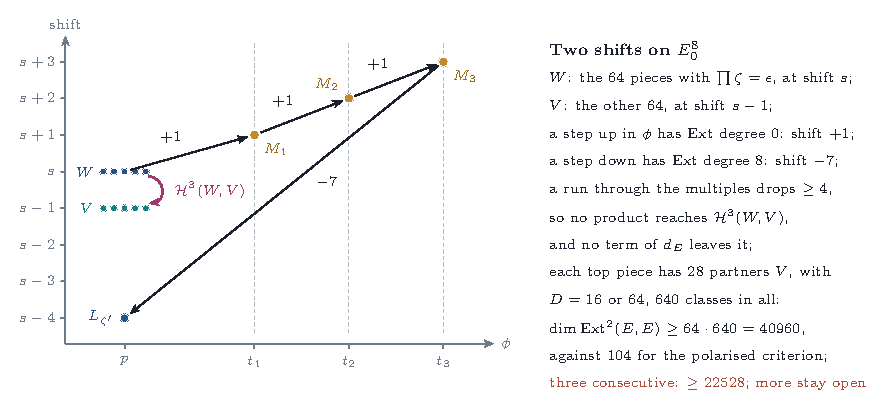
\includegraphics[width=\textwidth]{fig_efourshifts}
\caption{\Cref{lem:efourshifts} and \Cref{thm:efourtwolevels}, in the
placement $p<t_{1}<t_{2}<t_{3}$. Horizontal: the value $\phi$ of a piece;
vertical: its shift. The pieces $L_{\zeta}$ with $\prod\zeta=\epsilon$ sit at
the shift $s$ and the others at $s-1$. A run through the multiples, up three
times with $\Ext$ degree $0$ and down once with $\Ext$ degree $8$, ends four
shifts lower, the least drop of \Cref{lem:efourshifts}(iii), so it never
joins a top piece $W$ to a partner $V$ one shift lower; the group
$\mathcal{H}^{3}(W,V)$ survives in $\Ext^{2}(E,E)$.}
\label{fig:efourshifts}
\end{figure}

\Cref{fig:efourshifts} draws the shifts along a run. The hypothesis of (ii) is the arrangement of the explicit convolution of
\Cref{prop:explicitconvolution} at $n=3$, where the sixteen pieces of each
parity share a shift. The pieces
must not be twisted by line bundles of degree zero here, unlike in
\Cref{thm:noconvolution}: a twist that is nontrivial on the surface where
$\zeta$ and $\zeta'$ agree removes $\cH(L_{\zeta},L_{\zeta'})$.

With a third shift, a component of $\Ext$ degree two can follow or precede
a class of $\cH^{3}(L_{\zeta},L_{\zeta'})$, so the differential no longer
vanishes on these classes. When the three shifts are consecutive, such terms
reach only the groups
between the highest and the lowest shift, which are too small to remove the
classes.

\begin{theorem}[Three consecutive shifts on $E_{0}^{8}$]
\label{thm:efourthreelevels}
Keep \Cref{lem:efourshifts}, and suppose that the shifts of the $L_{\zeta}$
lie in $\{s,s-1,s-2\}$ for an integer $s$. By their parities, for a sign
$\epsilon$, the pieces with $\prod\zeta=\epsilon$ have the shift $s-1$ and
the others the shift $s$ or $s-2$; let $T$ and $B$ be the sets of pieces of
the shifts $s$ and $s-2$. Then, for every order of the pieces, every choice
of the shifts of the $M_{i}$ and every placement of the $t_{i}$:
\begin{enumerate}[label=\textup{(\roman*)},leftmargin=2.6em,itemsep=2pt]
\item every two pieces $L_{\zeta}$, $L_{\zeta'}$ that differ in exactly three
  coordinates have shifts differing by one, and the groups
  $\cH^{3}(L_{\zeta},L_{\zeta'})$ of \Cref{thm:efourtwolevels}, taken from
  the piece of the larger shift, have dimensions adding up to $40960$;
\item $d_{E}$ maps the sum of these groups into
  $\bigoplus_{c\in T,\,e\in B}\cH^{5}(c,e)$, and on them it consists of cup
  products with a single component of $\Ext$ degree two;
\item
  \[
    \dim\Ext^{2}(E,E)\;\ge\;40960-\sum_{c\in T,\,e\in B}\dim\cH^{5}(c,e)
    \;\ge\;40960-18432=22528 .
  \]
\end{enumerate}
In particular $E$ does not meet the polarised criterion. When $T$ or $B$ is
empty this is \Cref{thm:efourtwolevels}(ii).
\end{theorem}

\begin{proof}
(i) The ratios $\zeta'_{j}/\zeta_{j}$ in the three coordinates have
product $-1$, so the two pieces have opposite parities: one has the shift
$s-1$ and the other $s$ or $s-2$. Each of the $64$ pieces of the shift $s-1$
has $28$ such partners, whose groups have dimensions adding up to $640$, as
in the proof of \Cref{thm:efourtwolevels}; this gives $64\cdot640=40960$.

(ii) Let $x\in\cH^{3}(a,b)$ with $d_{a}=d_{b}+1$. As in the proof of
\Cref{thm:efourtwolevels}(ii), a term of $d_{E}(x)$ runs along chains of
components $c\to\dots\to a$ and $b\to\dots\to e$, not both empty, and lands
in $\cH(c,e)$ in $\Ext$ degree $3+d_{c}-d_{e}$. The shifts of the pieces
$L_{\zeta}$ differ by at most two, so by \Cref{lem:efourshifts}(iii) no part
of a chain between two pieces $L_{\zeta}$ passes through a multiple. Hence a
chain $c\to\dots\to a$ that starts at a multiple $M_{i}$ is a run
$M_{i}=m_{0}\to\dots\to m_{r}\to L_{1}$ of distinct multiples, $r\le2$,
followed by pieces $L_{\zeta}$ only; let $U_{1}$ and $D_{1}$ be the numbers
of its steps up and down the value $\phi$ before $L_{1}$, so that
$d_{L_{1}}=d_{M_{i}}+U_{1}-7D_{1}$ by \Cref{lem:efourshifts}(ii) and
$U_{1}+D_{1}=r+1\le3$. Likewise a chain $b\to\dots\to e$ ending at a multiple
$M_{k}$ ends with a run from a piece $L_{2}$ with $U_{2}$ steps up and $D_{2}$
down, $U_{2}+D_{2}\le3$ and $d_{M_{k}}=d_{L_{2}}+U_{2}-7D_{2}$. Put
$L_{1}=c$ if $c$ is a piece $L_{\zeta}$ and $L_{2}=e$ if $e$ is one, and
$\delta=d_{L_{1}}-d_{L_{2}}$; then $1=d_{a}-d_{b}\le\delta\le2$.

If $c$ and $e$ are both pieces $L_{\zeta}$, each nonempty chain lowers the
shift by at least one, so $3+d_{c}-d_{e}\ge5$, while $\delta\le2$ gives at
most $5$. So the degree is $5$, $c\in T$, $e\in B$, and the two chains
together consist of one component, of $\Ext$ degree two by
\Cref{lem:efourshifts}(i): the term is a cup product of $x$ with that
component.

If $c=M_{i}$ and $e$ is a piece $L_{\zeta}$, the degree is
$3+\delta-U_{1}+7D_{1}$, and $\cH(c,e)$ sits in degree $0$ or $8$ by
\Cref{lem:efourshifts}(ii). Degree $0$ needs $U_{1}\ge3+\delta\ge4$, and
degree $8$ needs $7D_{1}-U_{1}=5-\delta\in\{3,4\}$, so $D_{1}\ge1$ and
$U_{1}\ge3$; both contradict $U_{1}+D_{1}\le3$. The case of a piece $c$ and
a multiple $e$ is the same with the second run.

If $c=M_{i}$ and $e=M_{k}$, the degree is $3+\delta-U+7D$ with
$U=U_{1}+U_{2}\le6$ and $D=D_{1}+D_{2}$. For $i=k$ it is $3$, so
$U-7D=\delta\ge1$; $D=0$ is impossible, since the values would increase from
$t_{i}$ to $p$ along the first run and from $p$ to $t_{i}$ along the second,
and $D\ge1$ gives $U\ge8$. For $i\ne k$, $\cH(c,e)$ sits in degree $0$ if
$t_{k}>t_{i}$ and $8$ if $t_{k}<t_{i}$. Degree $0$ needs $U=3+\delta+7D$,
so $D=0$ and $U\ge4$; but then the multiples of the first run have values
below $p$ and those of the second values above $p$, so they are distinct and
$U\le3$. Degree $8$ needs $7D-U=5-\delta$, so $D=1$ and $U\ge3$: the runs
have at least four steps, so some multiple lies on both. One run increases
strictly. If it is the second, its values lie in $(p,t_{k}]$, while those of
the first lie at or above $t_{i}>t_{k}$ before its step down and below $p$
after it. If it is the first, its values lie in $[t_{i},p)$, while those of
the second lie above $p$ before its step down and at or below $t_{k}<t_{i}$
after it. Either way no multiple lies on both runs, a contradiction.

(iii) By \Cref{thm:efourtwolevels}(i), which holds for every convolution, no
coboundary has a component in these groups, so the kernel of $d_{E}$ on
their sum injects into $\Ext^{2}(E,E)$, and by (ii) its dimension is at
least $40960$ minus the dimension of the targets. For pieces $c$, $e$ of the
same parity, $\cH^{5}(c,e)$ is nonzero only when they differ in two or three
coordinates, and each piece has such partners with groups $\cH^{5}$ of
dimensions adding up to $960$.\footnote{The ratios $e_{j}/c_{j}\ne1$ have
product $1$. In two coordinates they are $(-1,-1)$, with $D=16$, or
$(i,-i)$, $(-i,i)$, with $D=4$; then
$\cH^{5}=\cH^{1}\otimes\cH^{1}\otimes\cH^{3}(B_{j}\times B_{k},\cO)$ has
dimension $4D$, and the six pairs of coordinates give
$6\cdot64+12\cdot16=576$. In three coordinates they are a permutation of
$(i,i,-1)$ or of $(-i,-i,-1)$, with $D=16$, and
$\cH^{5}=(\cH^{1})^{\otimes3}\otimes H^{2}(B_{l},\cO)$ has dimension $16$;
the four triples give $4\cdot6\cdot16=384$. In four coordinates
$\cH(c,e)$ sits in degree $4$.}\enlargethispage{3pt} So the sum in (iii) is at most
$\min(|T|,|B|)\cdot960\le32\cdot960=30720$, which already gives
$\dim\Ext^{2}(E,E)\ge10240$. The dimension of $\cH^{5}(c,e)$ depends only on
the ratio $e/c$, so the sum is the weight of the cut $(T,B)$ of a weighted
Cayley graph on the group of ratios of two pieces of one parity, of order
$64$ and degree $960$. For the vector $x=\pm1$ of the cut, the weight is
$\tfrac14\bigl(64\cdot960-x^{\mathsf T}Ax\bigr)\le16\,(960-\lambda)$, with
$A$ the weighted adjacency matrix and $\lambda$ its least eigenvalue. Its
eigenvalues are the character sums $\sum_{g}\dim\cH^{5}(1,g)\,\chi(g)$. A
character is $\chi(g)=\prod_{j}g_{j}^{k_{j}}$ with $k\in(\ZZ/4)^{4}$, up to
adding $(1,1,1,1)$; put $\omega_{j}=i^{k_{j}}$, $W=\sum_{j}\omega_{j}$,
$\varrho=\sum_{j}\omega_{j}^{2}$ and $\Omega=\prod_{j}\omega_{j}$. By the
list in the footnote, the ratios that move the pair of coordinates
$\{j,l\}$ contribute $64\,\omega_{j}^{2}\omega_{l}^{2}
+32\,\Re(\omega_{j}\bbar\omega_{l})$, and those that fix only the
coordinate $o$ contribute $32\,\Re\bigl(\Omega\bbar\omega_{o}(W-\omega_{o})\bigr)$.
Summing,
\[
  \chi\bigl(\textstyle\sum_{g}\dim\cH^{5}(1,g)\,g\bigr)
  =32\varrho^{2}+16|W|^{2}-192+32\,\Re(\Omega)\bigl(|W|^{2}-4\bigr).
\]
If $\Re\Omega=0$, the sum of the $k_{j}$ is odd, so an odd number of them
are odd, $|\varrho|=2$, and the value is at least $-64$. If $\Re\Omega=1$,
an even number are odd: with none or four, $|\varrho|=4$ and the value is at
least $192$; with two, $\varrho=0$, and $W=0$ would force the $k_{j}$ to be
$0,1,2,3$, whose sum is not divisible by $4$, so $|W|^{2}\ge4$ and the value
is at least $-128$. If $\Re\Omega=-1$, the value is
$32\varrho^{2}-16|W|^{2}-64$, and $|W|^{2}\le8+2\varrho^{2}$: when all
$k_{j}$ have the same parity, $|W|\le4=|\varrho|$, and when two are odd,
$\varrho=0$ and $W$ is a sum of two of $\pm1$ and two of $\pm i$, so
$|W|^{2}\le8$. Hence $\lambda\ge-192$,\footnote{The eight values are $960$,
$384$, $192$, $96$, $-32$, $-64$, $-128$ and $-192$. The bound $18432$ is
attained by the cut $\zeta_{3}\zeta_{4}\in\{1,i\}$ against
$\zeta_{3}\zeta_{4}\in\{-1,-i\}$, so $22528$ is the best bound that this
count gives.} and the sum is at most $16\cdot1152=18432$.
\end{proof}

\Cref{fig:efourthree} draws the three shifts and the budget.

\begin{figure}[tbp]
\centering
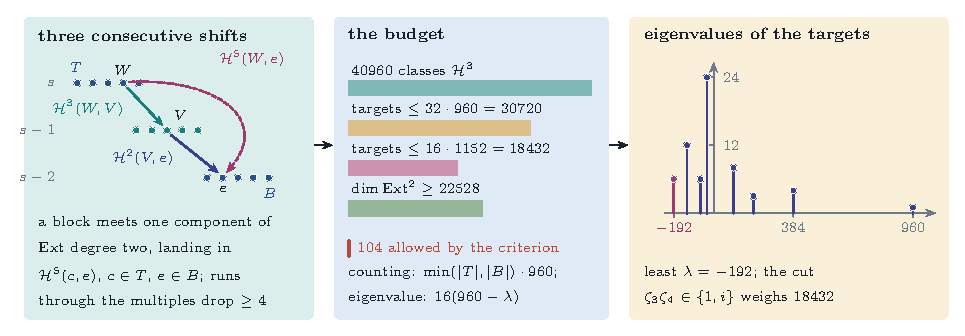
\includegraphics[width=\textwidth]{fig_efourthree}
\caption{\Cref{thm:efourthreelevels}. Left: the pieces $L_{\zeta}$ at three
consecutive shifts, those of one parity at $s-1$ and the others split between
$T$ at $s$ and $B$ at $s-2$; a group $\cH^{3}$ between two pieces that differ
in three coordinates (teal) can meet a component of $\Ext$ degree two
(indigo) only in a group $\cH^{5}(c,e)$ with $c\in T$ and $e\in B$ (magenta).
Middle: the $40960$ classes against the targets, at most $30720$ by counting
and $18432$ by the least eigenvalue, against the $104$ that the criterion
allows. Right: the eigenvalues of the Cayley graph of the targets.}
\label{fig:efourthree}
\end{figure}

The groups of \Cref{thm:efourtwolevels} join two pieces whose shifts differ
by one. All groups between pieces whose shifts differ by three, and thirteen
kinds between pieces whose shifts differ by two, are also left alone by the
differential, and with them the argument covers every
arrangement of the shifts within five consecutive values. For pieces $a$ and
$b$ call $d_{a}-d_{b}$ the \emph{spread} of $\cH(a,b)$; its classes of degree
two have $\Ext$ degree $2+d_{a}-d_{b}$. For $\zeta,\zeta'\in\mu_{4}^{4}$ call
$\zeta'/\zeta=(\zeta'_{j}/\zeta_{j})_{j}$ their \emph{ratio}; it
\emph{moves} the coordinates where it differs from $1$, and it changes the
parity, $\prod\zeta'=-\prod\zeta$, exactly when the product of its entries is
$-1$. As before,
$D(\zeta,\zeta')=\prod_{\zeta_{j}\ne\zeta'_{j}}|\zeta_{j}-\zeta'_{j}|^{2}$.

\begin{lemma}[Groups of spread two and three]\label{lem:efourspread}
Keep \Cref{lem:efourshifts}, and let $E$ be any convolution of the
$L_{\zeta}$ and the $M_{i}$, in any order, with any shifts of the given
parities and any placement of the $t_{i}$.
\begin{enumerate}[label=\textup{(\roman*)},leftmargin=2.6em,itemsep=2pt]
\item For a class $x$ of degree two in $\cH(L_{\zeta},L_{\zeta'})$ of
  positive spread, every term of $d_{E}(x)$ has all its leaves between
  pieces $L_{\zeta''}$.
\item Let $\prod\zeta=\prod\zeta'$, let $\zeta'/\zeta$ move all four
  coordinates, one of them by $-1$, and let $d_{L_{\zeta}}=d_{L_{\zeta'}}+2$.
  The classes of degree two of $\cH(L_{\zeta},L_{\zeta'})$ form
  $\cH^{4}(L_{\zeta},L_{\zeta'})$, of dimension $D(\zeta,\zeta')\in\{64,256\}$;
  no element of degree one has a differential with a nonzero component in
  it, and $d_{E}$ vanishes on it.
\item Let $\prod\zeta=-\prod\zeta'$ and $d_{L_{\zeta}}=d_{L_{\zeta'}}+3$. The
  classes of degree two of $\cH(L_{\zeta},L_{\zeta'})$ lie in
  $\cH^{5}(L_{\zeta},L_{\zeta'})$, and $d_{E}$ vanishes on them.
\item Let $\zeta$ and $\zeta'$ differ in exactly three coordinates, with
  $d_{L_{\zeta}}=d_{L_{\zeta'}}+1$. Every term of $d_{E}$ on
  $\cH^{3}(L_{\zeta},L_{\zeta'})$ runs along chains of components
  $c\to\dots\to L_{\zeta}$ and $L_{\zeta'}\to\dots\to e$ between pieces
  $L_{\zeta''}$ that together lower the shift by one or two.
\end{enumerate}
\end{lemma}

\begin{proof}
Write $a=L_{\zeta}$, $b=L_{\zeta'}$ and $\delta=d_{a}-d_{b}$. As in the proof
of \Cref{thm:efourtwolevels}(ii), a term of $d_{E}$ on a class of degree two
in $\cH(a,b)$ runs along chains of components $c\to\dots\to a$ and
$b\to\dots\to e$, not both empty, and lands in $\cH(c,e)$ in $\Ext$ degree
$3+d_{c}-d_{e}$, which is $3$ if $c=e$.

(i) Let $L_{1}$ be the first piece $L_{\zeta''}$ of the first chain and
$L_{2}$ the last of the second, and put
$X=(d_{L_{1}}-d_{a})+(d_{b}-d_{L_{2}})$. By \Cref{lem:efourshifts}(iii),
$X\ge0$, and $X\ge4$ if a multiple lies between $L_{1}$ and $a$ or between
$b$ and $L_{2}$. Before $L_{1}$ the first chain is a run of distinct
multiples, with $U_{1}$ steps up and $D_{1}$ steps down the value $\phi$ and
$U_{1}+D_{1}\le3$; after $L_{2}$ the second chain is a run with $U_{2}$ and
$D_{2}$ steps, $U_{2}+D_{2}\le3$. By \Cref{lem:efourshifts}(ii) the term has
$\Ext$ degree $3+\delta+X-U+7D$, where $U=U_{1}+U_{2}$ and $D=D_{1}+D_{2}$.
If $c$ and $e$ are pieces, this is $3+\delta+X$; a multiple on a chain makes
it at least $8$, but $\cH^{8}(c,e)\ne0$ only for $c=e$, where the degree is
$3$. If $c=M_{i}$ and $e$ is a piece, $\cH(c,e)$ sits in degree $0$ if
$t_{i}<p$ and in degree $8$ if $t_{i}>p$. Degree $0$ needs
$U_{1}\ge3+\delta+X\ge4$. Degree $8$ needs a step down on the run from
$t_{i}$ to $p$, so $D_{1}\ge1$, and then
$U_{1}=7D_{1}-5+\delta+X\ge3$. Both contradict $U_{1}+D_{1}\le3$, and a
piece $c$ with a multiple $e$ is the same. Let $c=M_{i}$ and $e=M_{k}$. For
$i=k$ the degree is $3$, so $U-7D=\delta+X\ge1$; $D\ge1$ would give $U\ge8$,
and $D=0$ would make the values increase from $t_{i}$ to $p$ and then from
$p$ to $t_{i}$. For $i\ne k$, $\cH(c,e)$ sits in degree $0$ if $t_{k}>t_{i}$
and in degree $8$ if $t_{k}<t_{i}$. Degree $0$ needs $U=3+\delta+X+7D$, so
$D=0$ and $U\ge4$; but then the first run lies below $p$ and the second
above, so the multiples are distinct and $U\le3$. Degree $8$ needs $D\ge1$,
since with $D=0$ the values would satisfy $t_{i}<p<t_{k}$; then
$7D-U=5-\delta-X\le4$ gives $D=1$ and $U\ge3$, so the runs have at least
four steps and share a multiple, which the last paragraph of the proof of
\Cref{thm:efourthreelevels}(ii) excludes.

(ii) By the proof of \Cref{lem:efourshifts}(i), $\cH(a,b)$ is the tensor
product of four groups $H^{1}$ and sits in degree $4$, of dimension
$D(\zeta,\zeta')$; the ratio is $(-1,-1,-1,-1)$, with $D=256$, or a
permutation of $(i,-i,-1,-1)$, with $D=64$.\footnote{A ratio that moves
every coordinate has entries in $\{i,-1,-i\}$ and product $1$. With a $-1$
among them it is $(-1,-1,-1,-1)$ or has exactly two entries $-1$ and the
entries $i$ and $-i$, twelve ratios; together thirteen, and
$256+12\cdot64=1024$. The other eight ratios have all four entries in
$\{i,-i\}$ and $D=16$; (ii) makes no statement about them.}\enlargethispage{3pt} A coboundary with a component in $\cH(a,b)$ is
a sum of terms of \Cref{lem:harmonicmodel}(iii) along a path
$a\to\dots\to b$ of morphisms of degree one, one of them an element $u$ and
the others components, that lowers the shift by two. By
\Cref{lem:efourshifts}(iii) no multiple lies on it, and by
\Cref{lem:efourshifts}(i) each step between distinct pieces lowers the shift
by at least one. So the path consists of a component of $\Ext$ degree three
from $a$ to $b$, which lies in $\cH^{3}(a,b)=0$, and a class of
$\cH^{1}(a,a)$ or $\cH^{1}(b,b)$; or of two steps $a\to c\to b$ of $\Ext$
degree two, possibly with a class of $H^{1}(A,\cO_{A})$ at one of the three
pieces. The output has degree one on every surface. Without the class of
$H^{1}$ the two steps have degrees adding up to one on every surface, so they
move disjoint pairs of coordinates and have degree zero elsewhere; a step of
$\Ext$ degree two changes the parity, so its two moved entries have product
$-1$ and are $(i,i)$ or $(-i,-i)$, and $\zeta'/\zeta$ has no entry $-1$.
With the class of $H^{1}$, \Cref{lem:degreedrop} gives a drop of one on a
surface where all three leaves have positive degree, and the output has
degree at least two there.

Now let a term of $d_{E}$ on $\cH^{4}(a,b)$ carry the components
$y_{1},\dots,y_{m}$, $m\ge1$, between pieces by (i), and land in
$\cH(c,e)$; let $K$ be the set of coordinates fixed by the ratio of $c$ and
$e$, and $X\ge m$ the drop of the chains. The output has $\Ext$ degree
$5+X$. Let $n_{j}$ be the number of the $y_{i}$ of positive degree on
$B_{j}$; the class $x$ has degree one there, so \Cref{lem:degreedrop} bounds
the drop on $B_{j}$ by $\max(0,n_{j}-1)$. For $j\notin K$ the output has
degree $1$ on $B_{j}$, so the degrees of the $y_{i}$ there add up to at most
$\max(0,n_{j}-1)$, which forces $n_{j}=0$. For $j\in K$ the $y_{i}$ undo the
entry $\zeta'_{j}/\zeta_{j}\ne1$, so $n_{j}\ge1$, and the output has degree
at least $1+n_{j}-(n_{j}-1)=2$ there, hence exactly $2$. So
$5+X=(4-|K|)+2|K|$, that is $X=|K|-1$. The components change the parity
$X$ times modulo two, and together their ratio is $\zeta/\zeta'$ on $K$ and
$1$ elsewhere, so
\[
  \prod_{j\in K}\zeta'_{j}/\zeta_{j}=(-1)^{|K|-1}.
\]
For the ratio $(-1,-1,-1,-1)$ the left side is $(-1)^{|K|}$. For a
permutation of $(i,-i,-1,-1)$ the left side is real only if $K$ contains
both or neither of the coordinates moved by $\pm i$, and then it is again
$(-1)^{|K|}$. So no term is nonzero.

(iii) The classes of degree two have $\Ext$ degree $5$. By (i) a term of $d_{E}$ on them lands
in $\Ext$ degree $6+X$, with $X\ge1$ the drop of the chains between pieces.
For $X\ge2$ this is at least $8$, which needs $c=e$ and degree $3$. For $X=1$
the pieces $c$, $e$ have shifts differing by four, hence the same parity, so
their ratio moves at least two coordinates and $\cH(c,e)$ has no degree above
$6$.

(iv) By (i) a term lands in $\Ext$ degree $4+X$, with $X\ge1$ the drop of the
chains between pieces. For $X\ge4$ the degree is at least $8$, which needs
$c=e$. For $X=3$ the degree is $7$, which needs a ratio moving one
coordinate, hence opposite parities, while $d_{c}-d_{e}=4$ is even.
\end{proof}

The groups of (ii) are reached by no coboundary and left by no term in every
convolution, so they survive in $\Ext^{2}(E,E)$ as soon as the shifts give
them the spread two. That happens along every edge of a Cayley graph that
crosses between two shift values of one parity, and a cut of that graph is
never light.

\begin{lemma}[Cuts of a Cayley graph]\label{lem:cayleycut}
Let $G$ be a finite abelian group, $S\subset G\setminus\{0\}$ a generating
set and $w\colon S\to\RR_{>0}$ a weight, extended by $0$ to $G$. For every
subset $T\subset G$ with $T\ne\emptyset,G$,
\[
  \sum_{c\in T,\ e\notin T}w(e-c)\;\ge\;\min_{H}\,|H|\cdot w(S\setminus H),
\]
the minimum over the proper subgroups $H$ of $G$. For the group $G_{0}$ of
the $64$ ratios of pieces of one parity, with $S$ the thirteen ratios of
\Cref{lem:efourspread}(ii) and $w=D$, the minimum is $1024$, attained only at
$H=0$, so every such cut weighs at least $1024$.
\end{lemma}

\begin{proof}
The left side is $\sum_{s\in S}w(s)\,|(T+s)\setminus T|$. Let $H$ be the
stabiliser of $T$, a proper subgroup since $T\ne\emptyset,G$. Then $T$ and
$T+s$ are unions of cosets of $H$, and for $s\notin H$ the set
$(T+s)\setminus T$ is nonempty, since $|T+s|=|T|$, so it has at least $|H|$
elements. This gives the inequality. In $G_{0}$, written additively as the
quadruples in $(\ZZ/4)^{4}$ of sum $0$, the ratios of type $(i,-i,-1,-1)$
generate, since the differences of two of them give every $e_{j}-e_{k}$. The
weights are $256$ once and $64$ otherwise, and $|S\cap H|\le|H|-1$. So
$|H|\,w(S\setminus H)$ is $1024$ for $H=0$, at least
$|H|\,(1024-256-64(|H|-2))$, which is $1536$, $2560$ and $3072$, for
$|H|=2,4,8$, and at least $64|H|\ge1024$ for $|H|\ge16$, because some
generator lies outside $H$.\footnote{The orders of the subgroups of
$G_{0}\cong(\ZZ/4)^{3}$ are powers of two. A cut at one vertex weighs exactly
$1024$, so the bound is sharp.}
\end{proof}

\begin{theorem}[One parity at two or three values]\label{thm:efourspreadtwo}
Keep \Cref{lem:efourshifts}, and suppose that the shifts of the pieces
$L_{\zeta}$ with $\prod\zeta=\epsilon$ take exactly two values $s$ and $s-2$,
or exactly three values $s+2$, $s$ and $s-2$, for a sign $\epsilon$ and an
integer $s$. Then, for every order of the pieces, all shifts of the other
pieces, every choice of the shifts of the $M_{i}$ and every placement of the
$t_{i}$,
\[
  \dim\Ext^{2}(E,E)\;\ge\;1024 .
\]
In particular $E$ does not meet the polarised criterion.
\end{theorem}

\begin{proof}
Let $T$ be the set of pieces of parity $\epsilon$ at the shift $s$; it is
neither empty nor all of them. Two pieces of parity $\epsilon$, one in $T$
and the other not, have shifts differing by exactly two. When their ratio is
one of the thirteen of \Cref{lem:efourspread}(ii), the group $\cH^{4}$ from
the piece of the larger shift to the other is reached by no coboundary and
killed by no term, so its classes inject into $\Ext^{2}(E,E)$, and those of
different pairs lie in different summands $\cH(a,b)$. Their dimensions add up
to the weight of the cut $(T,\complement T)$ of the Cayley graph of
\Cref{lem:cayleycut}, since the pieces of parity $\epsilon$ form a coset of
$G_{0}$; so they add up to at least $1024$.
\end{proof}

\begin{theorem}[Shifts three apart]\label{thm:efourspreadthree}
Keep \Cref{lem:efourshifts}, and suppose that the pieces $L_{\zeta}$ with
$\prod\zeta=\epsilon$ all have the shift $s$ and the others have shifts in
$\{s-3,s+3\}$. Then, for every order, every choice of the shifts of the
$M_{i}$ and every placement of the $t_{i}$,
\[
  \dim\Ext^{2}(E,E)\;\ge\;64\cdot1072-128\cdot8=67584 .
\]
\end{theorem}

\begin{proof}
Every piece $W$ of parity $-\epsilon$ and every piece $V$ of parity $\epsilon$
have shifts differing by three. By \Cref{lem:efourspread}(iii) the classes
of degree two of the group from the higher to the lower of the two lie in
$\cH^{5}$, and $d_{E}$ vanishes on them. For each $W$ these groups have
dimensions adding up to $1072$.\footnote{Let the ratio move $k$
coordinates. For $k=1$ it is $-1$ in one coordinate, $D=4$, and $\cH^{5}$
is $H^{1}$ tensored with the part of degree four of $H^{*}(\cO)$ on the
other three surfaces, of dimension $\binom{6}{4}=15$: four partners with
$60$ each. For $k=2$ it is $(i,i)$ or $(-i,-i)$, $D=4$, and the part of
degree three on the other two surfaces has dimension $\binom43=4$: twelve
partners with $16$ each. For $k=3$ the part of degree two on the last surface
has dimension one, and the $28$ partners give $640$ as in
\Cref{thm:efourtwolevels}. For $k=4$ the group sits in degree $4$. So
$240+192+640=1072$.} A coboundary with a component in such a group runs
along a path of morphisms of degree one that lowers the shift by three;
no multiple lies on it, by \Cref{lem:efourshifts}(iii), and a step between
distinct pieces lowers the shift by at least one, while no piece has a shift
strictly between those of $W$ and $V$. So the path is the component between
$W$ and $V$ together with a class of $H^{1}(A,\cO_{A})$ at one of them, and
the components of all coboundaries in these groups come from
$\bigoplus_{a}\cH^{1}(a,a)$ over the $128$ pieces, of dimension
$128\cdot8=1024$. The $64\cdot1072=68608$ classes are cocycles, and at most
$1024$ dimensions of them are coboundaries.
\end{proof}

When one parity sits at a single shift, the groups $\cH^{3}$ of
\Cref{thm:efourtwolevels} survive next to it unless pieces of the other
parity crowd it from both sides.

\begin{proposition}[A gap of four]\label{prop:efourgap}
Keep \Cref{lem:efourshifts}, let the pieces $L_{\zeta}$ with
$\prod\zeta=\epsilon$ all have the shift $y$, and let $T$ be the set of
pieces of parity $-\epsilon$ at the shift $y+1$. If $T$ is not empty and no
piece has the shift $y-1$ or $y+3$, then for every order, every choice of
the shifts of the $M_{i}$ and every placement of the $t_{i}$, the groups
$\cH^{3}(W,V)$ with $W\in T$ and $V$ differing from $W$ in exactly three
coordinates are reached by no coboundary and killed by no term, and
\[
  \dim\Ext^{2}(E,E)\;\ge\;640\,|T|\;\ge\;640 .
\]
The same holds with $y+1$, $y-1$, $y+3$ replaced by $y-1$, $y+1$, $y-3$ and
the groups $\cH^{3}(V,W)$.
\end{proposition}

\begin{proof}
By \Cref{thm:efourtwolevels}(i), which holds for every convolution, no
coboundary reaches these groups. By \Cref{lem:efourspread}(iv) a term of
$d_{E}$ on $\cH^{3}(W,V)$ runs along chains of components between pieces
into $W$ and out of $V$ that lower the shift by one or two in all; the
first would pass through a piece at the shift $y+2$ or $y+3$, the second
through one at $y-1$ or $y-2$. The shifts $y\pm2$ have parity $\epsilon$,
whose pieces are all at $y$, and $y-1$, $y+3$ are excluded. Each $W\in T$
has $28$ partners $V$, all at the shift $y$, with groups of dimensions adding
up to $640$. The second statement has the same proof, with the chains into
$V$ and out of $W$ in place of those into $W$ and out of $V$.
\end{proof}

\begin{corollary}[Five consecutive shifts]\label{cor:efourfive}
Keep \Cref{lem:efourshifts}. If the shifts of the $128$ pieces $L_{\zeta}$
lie in five consecutive integers, then, for every order, every choice of the
shifts of the $M_{i}$ and every placement of the $t_{i}$,
$\dim\Ext^{2}(E,E)\ge640$; no such convolution meets the polarised
criterion.
\end{corollary}

\begin{proof}
Let the values be $s,\dots,s-4$, with one parity at values in
$\{s,s-2,s-4\}$ and the other at values in $\{s-1,s-3\}$. If the second
parity takes both its values, or the first takes two values two apart or all
three, \Cref{thm:efourspreadtwo} applies. Otherwise the second parity sits at
one value $y$ and the first at one value or at $\{s,s-4\}$. One value each,
at an odd distance at most three: \Cref{thm:efourtwolevels} or
\Cref{thm:efourspreadthree}. The first at $\{s,s-4\}$: for $y=s-1$ the
pieces at $y+1=s$ are not empty and $y-1$, $y+3$ are empty, and for $y=s-3$
the pieces at $y-1=s-4$ are not empty and $y+1$, $y-3$ are empty, so
\Cref{prop:efourgap} applies. The least of the bounds is $640$.
\end{proof}

Within six consecutive values two arrangements are left, up to exchanging
the parities: each parity at one shift, five apart, and the parities at
$\{s,s-4\}$ and $\{s-1,s-5\}$. The first is settled by the diagonal, whose
classes at a shift with no other piece nearby can be reached only through
all three multiples, and the second by the groups of
\Cref{thm:efourtwolevels} once more.

\begin{lemma}[The diagonal at a lonely shift]\label{lem:efourlonely}
Keep \Cref{lem:efourshifts}, and let the pieces $L_{\zeta}$ with
$\prod\zeta=\epsilon$ all have the shift $s$ and the others the shift $s-g$,
for a sign $\epsilon$ and an odd integer $g\ge5$. Let $y\in\cH^{2}(a,a)$ be
a diagonal class at a piece $a$, and let a term of $d_{E}(y)$ in
\Cref{lem:harmonicmodel}(iii) be nonzero. Then $a$ is the only piece on its
path, the path passes through $M_{1}$, $M_{2}$ and $M_{3}$, and the shifts
of $a$, $M_{1}$, $M_{2}$, $M_{3}$ are pairwise incongruent modulo $4$.
\end{lemma}

\begin{proof}
Write the path as $c\to\dots\to a\to\dots\to e$, with the chain of
components into $a$ and the chain out of $a$ not both empty, so that
$c\ne e$, since the components of a convolution go up the order of the
pieces. Let $L_{1}$ and $L_{2}$ be the first and the last piece on it and
$X=d_{L_{1}}-d_{L_{2}}$; before $L_{1}$ and after $L_{2}$ the path is a run
of distinct multiples, with $U$ steps up and $D$ steps down the value $\phi$
in all. As in the proof of \Cref{lem:efourspread}(i), now with $\delta=0$,
the term has $\Ext$ degree $3+X-U+7D$ by \Cref{lem:efourshifts}(ii). A
sequence of components from one piece to another lowers the shift by
\Cref{lem:efourshifts}(iii), and the pieces have the shifts $s$ and $s-g$;
so $X\in\{0,g\}$, and $X=0$ exactly when $a$ is the only piece on the path.

If $c$ and $e$ are pieces, then $U=D=0$ and $X=g$, and $\cH^{3+g}(c,e)=0$
since $3+g\ge8$ and $c\ne e$. If $c$ is a multiple and $e$ a piece, then
$\cH(c,e)$ sits in degree $0$ or $8$. Degree $0$ needs $U=3+X+7D$, so
$X=D=0$ and $U=3$. Degree $8$ needs $7D-U=5-X$: for $X=0$ this gives $D=1$
and $U=2$; for $X=g$ it gives $D=0$ and $U=g-5$, which is at least one
because the run before $L_{1}$ is not empty and at most three, so $g=7$; but
then the path lowers the shift by seven from $L_{1}$ to $e$, by a single
component, of $\Ext$ degree eight between distinct pieces, or by a run
through multiples, and neither is possible.\footnote{Between distinct pieces
$\cH^{8}=0$. A run from a piece through $m\le3$ distinct multiples to a piece
has $m+1$ steps, at least one up and one down, and lowers the shift by
$7D'-U'$ with $U'+D'=m+1$: by $6$, $5$, $4$ for $D'=1$, by $13$, $12$ for
$D'=2$ and by $20$ for $D'=3$, never by seven.} A piece $c$ with a multiple $e$ is the same
with the runs exchanged. If $c$ and $e$ are multiples, both runs are
nonempty and together pass through at most three multiples, so $U+D\le3$
and $U+D\ge2$. Degree $0$ needs $U=3+X+7D$, so $X=D=0$ and $U=3$. Degree $8$
needs $7D-U=5-X$; $D=0$ gives $U=X-5\ge2$, so $X=g=7$, which is excluded as
before; $D=1$ gives $U=2+X\le2$, so $X=0$ and $U=2$; $D\ge2$ gives $U\ge9$.

So in every case $X=0$ and $U+D=3$: the path consists of $a$ and the three
multiples, with three steps. A step up raises the shift by one and a step
down lowers it by seven, so every step adds one modulo $4$, and the four
nodes of the path have the shifts $d_{c},d_{c}+1,d_{c}+2,d_{c}+3$ modulo $4$
in the order of the path.\footnote{With the values $t_{1}<t_{2}<t_{3}$ and
$p$, the path with $U=3$ visits the four nodes in the order of their values;
a path with $U=2$ and $D=1$ ending in degree eight visits the largest $j$
values in increasing order and then the others, $j=1,2,3$. So each placement
has exactly four such paths, and for each the shifts of the multiples are
determined by $d_{a}$.}
\end{proof}

\begin{proposition}[Single shifts]\label{prop:efoursingle}
Keep \Cref{lem:efourshifts}, and suppose that the pieces $L_{\zeta}$ with
$\prod\zeta=\epsilon$ all have the shift $s$ and the others all have the
shift $s-g$, for a sign $\epsilon$ and an odd integer $g$. Then, for every
order, every choice of the shifts of the $M_{i}$ and every placement of the
$t_{i}$,
\[
  \dim\Ext^{2}(E,E)\;\ge\;64\cdot28=1792 .
\]
\end{proposition}

\begin{proof}
Exchanging the parities, we may take $g>0$. For $g=1$ and $g=3$ this is
\Cref{thm:efourtwolevels} and \Cref{thm:efourspreadthree}. Let $g\ge5$. If a
term of $d_{E}$ were nonzero on a diagonal class at a piece of shift $s$ and
another on a diagonal class at a piece of shift $s-g$, then by
\Cref{lem:efourlonely} the shifts of the three multiples would be pairwise
incongruent modulo $4$ and miss both the residue of $s$ and that of $s-g$,
which differ, since $g$ is odd. So at one of the two shifts $d_{E}$ vanishes
on the $28$ diagonal classes of each of the $64$ pieces there, and by
\Cref{prop:nothingenters}, which holds for $n=4$, these $1792$ classes
inject into $\Ext^{2}(E,E)$.\footnote{The proof does not look at the classes
between the two parities. For $g=5$ these are $64\cdot16=1024$ classes of
degree two in groups $\cH^{7}$, on which $d_{E}$ vanishes by
\Cref{lem:efourspread}(i); but the coboundaries of the loops in
$\cH^{1}(a,a)$, and, when two multiples have suitable shifts, the products
along runs $W\to M_{i}\to M_{j}\to V$, reach them, and counting alone gives
nothing there.}
\end{proof}

\begin{proposition}[Interleaved shifts]\label{prop:efourpairs}
Keep \Cref{lem:efourshifts}, and suppose that the shifts of the pieces
$L_{\zeta}$ with $\prod\zeta=\epsilon$ take exactly the two values $s$ and
$s-4$, and those of the others exactly the two values $s-1$ and $s-5$. Then,
for every order, every choice of the shifts of the $M_{i}$ and every
placement of the $t_{i}$, $\dim\Ext^{2}(E,E)\ge640$.
\end{proposition}

\begin{proof}
Let $A$ and $A'$ be the pieces of parity $\epsilon$ at the shifts $s$ and
$s-4$, and $B$ and $B'$ those of parity $-\epsilon$ at $s-1$ and $s-5$; all
four are nonempty. Let $W$ and $V$ differ in exactly three coordinates, with
$d_{W}=d_{V}+1$, that is $W\in A$ and $V\in B$, or $W\in A'$ and $V\in B'$.
By \Cref{thm:efourtwolevels}(i) no coboundary reaches $\cH^{3}(W,V)$, and by
\Cref{lem:efourspread}(iv) a term of $d_{E}$ on it passes through a piece at
the shift $d_{W}+1$ or $d_{W}+2$ or at $d_{V}-1$ or $d_{V}-2$. These are
$s+1$, $s+2$, $s-2$, $s-3$ for $W\in A$ and $s-3$, $s-2$, $s-6$, $s-7$ for
$W\in A'$, and no piece has these shifts. So the groups inject into
$\Ext^{2}(E,E)$.

Let $\Gamma$ be the group of the ratios of two pieces, of order $128$,
which acts simply transitively on the pieces, and $S_{3}\subset\Gamma$ the
$28$ ratios that move exactly three coordinates and change the parity, with
the weight $D$, which adds up to $640$ (\Cref{thm:efourtwolevels}). With
$X=A\cup B'$ the pairs above are exactly the edges of the Cayley graph of
$(\Gamma,S_{3})$ between $X$ and its complement $A'\cup B$; so the
dimensions add up to the weight of that cut, and $X$ is neither empty nor
everything. Written additively, as the quadruples in $(\ZZ/4)^{4}$ of even
sum, the differences of two ratios of type $(i,-i,-1,1)$ give every
$e_{j}-e_{k}$, which generate the quadruples of sum $0$ modulo $4$, and the
elements of $S_{3}$ have sum $2$ modulo $4$; so $S_{3}$ generates $\Gamma$.
In \Cref{lem:cayleycut},
$H=0$ gives $640$; for $|H|=2,4,8,16$ at most $|H|-1$ elements of $S_{3}$ lie
in $H$, at most four of them of weight $64$, so $|H|\,w(S_{3}\setminus H)$ is
at least $2\cdot576$, $4\cdot448$, $8\cdot336$ and $16\cdot208$; for
$|H|=32$ some $r\in S_{3}$ lies outside $H$, and so does $-r$, which gives
weight at least $32$, or $64$ if $r=-r$; and for $|H|=64$ the weight outside
$H$ is at least $16$. So every such cut weighs at least $640$.\footnote{The
subgroups of $\Gamma\cong(\ZZ/4)^{3}\times\ZZ/2$ have orders that are powers
of two. A cut at a single vertex weighs exactly $640$, so the bound is
sharp.}
\end{proof}

\begin{corollary}[Six consecutive shifts]\label{cor:efoursix}
Keep \Cref{lem:efourshifts}. If the shifts of the $128$ pieces $L_{\zeta}$
lie in six consecutive integers, then, for every order, every choice of the
shifts of the $M_{i}$ and every placement of the $t_{i}$,
$\dim\Ext^{2}(E,E)\ge640$; no such convolution meets the polarised
criterion.
\end{corollary}

\begin{proof}
By \Cref{cor:efourfive} we may assume that the shifts take both values $s$
and $s-5$ of the window $s,\dots,s-5$; let the parity at $s$ have its values
in $\{s,s-2,s-4\}$ and the other in $\{s-1,s-3,s-5\}$. If one of them takes
two values two apart, or three, \Cref{thm:efourspreadtwo} applies.
Otherwise the first takes $\{s\}$ or $\{s,s-4\}$ and the second $\{s-5\}$ or
$\{s-1,s-5\}$. For $\{s\}$ and $\{s-5\}$ this is \Cref{prop:efoursingle},
and for $\{s,s-4\}$ and $\{s-1,s-5\}$ it is \Cref{prop:efourpairs}. For
$\{s\}$ and $\{s-1,s-5\}$, \Cref{prop:efourgap} applies in its second form
with $y=s$: the shift $s-1$ is taken and $s+1$, $s-3$ are not. For
$\{s,s-4\}$ and $\{s-5\}$ it applies in its first form with $y=s-5$: the
shift $s-4$ is taken and $s-6$, $s-2$ are not. The least of the bounds is
$640$.
\end{proof}

For the arrangements outside these results the diagonal still carries a
large part of the obstruction.

\begin{proposition}[Cup products on the diagonal at $n=4$]
\label{prop:efourcupkernel}
Keep \Cref{lem:efourshifts}, so that $D^{2}$ has dimension $131\cdot28=3668$.
For every convolution the cup products vanish on the $84$ diagonal classes of
the $M_{i}$, and on the $3584$ diagonal classes of the $L_{\zeta}$ they have
a kernel of dimension at least $400$. So their kernel on $D^{2}$ has
dimension at least $484$, and a convolution meeting the polarised criterion
needs products of length at least three that remove at least $380$ diagonal
classes.
\end{proposition}

\begin{proof}
As in the proof of \Cref{prop:cupkernel}, the cup products in $\cH(a,b)$
are $(y_{a}-y_{b})\wedge\delta^{H}_{ab}$, they vanish on the classes of the
$M_{i}$, and for $L_{\zeta}$, $L_{\zeta'}$ and a type $\tau$ of degree two on
the four surfaces they vanish on the part of type $\tau$ unless $\zeta'/\zeta$
fixes the coordinates in the support of $\tau$. So a class whose part of type
$\tau$ depends only on the coordinates of $\zeta$ in the support of $\tau$
has vanishing cup products. The four types $(2,0,0,0)$ have dimension one and
four values of the coordinate, the six types $(1,1,0,0)$ have dimension four
and sixteen values of the two coordinates: $4\cdot4+6\cdot16\cdot4=400$. By
\Cref{prop:nothingenters}, which holds for $n=4$, the kernel of $d_{E}$ on
$D^{2}$ injects into $\Ext^{2}(E,E)$, and it is at most $104$ only if the
longer products remove $380$ dimensions of these $484$.
\end{proof}

\Cref{fig:efourspread} and \Cref{fig:efoursix} draw the
arrangements and the bounds.

\begin{figure}[tbp]
\centering
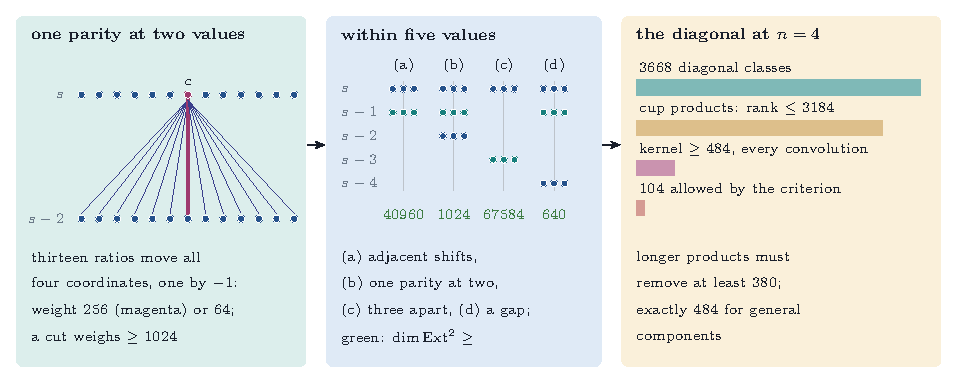
\includegraphics[width=\textwidth]{fig_efourspread}
\caption{The shift arrangements of the pieces $L_{\zeta}$ on $E_{0}^{8}$.
Left: one parity at two values two apart; a piece $c$ is joined to the
thirteen pieces whose ratio moves every coordinate, one by $-1$, and the
groups $\cH^{4}$ of the edges crossing between the values survive, weighing
at least $1024$ (\Cref{lem:efourspread}(ii), \Cref{lem:cayleycut}). Middle:
the four kinds of arrangement within five consecutive values, with the
result that excludes each and its bound on $\dim\Ext^{2}$. Right: the
diagonal at $n=4$; the cup products leave at least $484$ of the $3668$
classes, and the criterion allows $104$ (\Cref{prop:efourcupkernel}).}
\label{fig:efourspread}
\end{figure}

\begin{figure}[tbp]
\centering
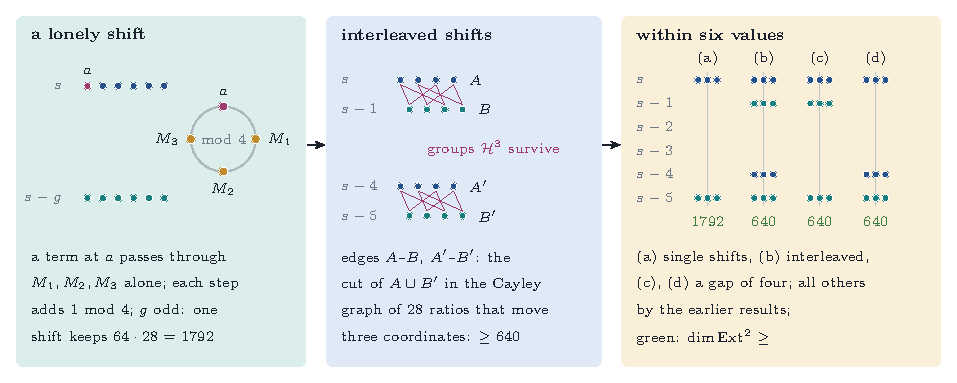
\includegraphics[width=\textwidth]{fig_efoursix}
\caption{The arrangements within six consecutive values on $E_{0}^{8}$.
Left: the parities at single shifts $s$ and $s-g$, $g$ odd and at least five;
a term on a diagonal class at a piece $a$ runs through $M_{1}$, $M_{2}$,
$M_{3}$ and no other piece, and since each step adds one to the shift modulo
$4$ the four nodes have distinct residues, so the multiples serve at most one
of the two shifts and the $1792$ diagonal classes at the other survive
(\Cref{lem:efourlonely}, \Cref{prop:efoursingle}). Middle: the interleaved
shifts; the groups $\cH^{3}$ between $A$ and $B$ and between $A'$ and $B'$
survive and form a cut of the Cayley graph of the $28$ ratios that move
three coordinates, of weight at least $640$ (\Cref{prop:efourpairs}).
Right: the four arrangements left within six values by the results for five
values, each with its bound on $\dim\Ext^{2}$ (\Cref{cor:efoursix}).}
\label{fig:efoursix}
\end{figure}

\begin{remark}[What the route gives]\label{rem:convolutionsopen}
At $n=3$ the route through convolutions of these pieces is decided. The
diagonal obstruction of \Cref{thm:esixdiagonal} leaves room only for the
fourfold products along one path, and the explicit convolution of
\Cref{prop:explicitconvolution} solves the Maurer--Cartan equation. The
obstruction that decides the route lies off the diagonal, in classes that no
product of any length can reach: those between pieces that differ in every coordinate and have
adjacent shifts (\Cref{lem:allthree}), and, at pieces whose shifts are not
adjacent to the shift of the paths, the classes of type $(1,1,0)$. No order
and no choice of shifts or twists avoids both, and
\Cref{thm:noconvolution} excludes every convolution of the $35$ pieces; in
the explicit convolution the first kind alone gives $2560$ classes against
the $57$ allowed. In each placement exactly two of the eight sign patterns
carry products, and the two are exchanged by a symmetry of the
construction.\footnote{The automorphism of $A$ that is $-1$ on the coordinate
$z_{n+1}$ and the identity on the others changes $\alpha$ into $-\alpha$,
fixes $\theta$ and permutes the $L_{\zeta}$, changing $\zeta_{1}$ into
$-\zeta_{1}$; composed with the shift $[1]$ it changes every $\sigma_{i}$
into $-\sigma_{i}$ and keeps everything else.} The member $E_{0}^{6}$ with
this Weil structure has trivial discriminant, where the Weil classes are
algebraic on every member by Markman's theorem \cite{Mar25a,Mar25b}, so a
convolution meeting the criterion here would have given a second proof of a
known case rather than a new one. At $n=4$ the classes between pieces that
differ in three coordinates and have adjacent shifts are again reached by
nothing, in every convolution, and when the pieces $L_{\zeta}$ occupy two
shifts, as in the explicit convolution, no term of $d_{E}$ leaves them, so
that $\dim\Ext^{2}(E,E)\ge40960$ against the $104$ allowed
(\Cref{thm:efourtwolevels}). With three consecutive shifts the
differential reaches these classes, but only through cup products into the
groups between the highest and the lowest shift, and at least $22528$ of
them survive (\Cref{thm:efourthreelevels}). The groups of spread three, and
those of spread two whose ratio moves every coordinate, one of them by $-1$,
are untouched as well, in every convolution
(\Cref{lem:efourspread}): the latter cross every cut between
two shift values of one parity, and weigh at least $1024$ there
(\Cref{thm:efourspreadtwo}); with one parity at a single shift, those of
spread three, or of spread one beside a gap, survive in their turn
(\Cref{thm:efourspreadthree}, \Cref{prop:efourgap}). Together they exclude
every convolution whose pieces $L_{\zeta}$ have their shifts within five
consecutive values (\Cref{cor:efourfive}). The two arrangements left within
six values fall as well: with each parity at a single shift, at any odd
distance, the diagonal classes at one of the two shifts can be reached only
through all three multiples, and the multiples serve at most one of them
(\Cref{lem:efourlonely}, \Cref{prop:efoursingle}); the interleaved shifts
leave the groups of \Cref{thm:efourtwolevels} on a cut
(\Cref{prop:efourpairs}). So every convolution whose shifts lie in six
consecutive values fails (\Cref{cor:efoursix}). For wider arrangements the
cup products still leave $484$ diagonal classes, so products of length at
least three would have to remove $380$ (\Cref{prop:efourcupkernel}), and
products of length three and four among the $L_{\zeta}$ pass every test of
\Cref{thm:esixdiagonal}. Whether some convolution of the $131$ pieces whose
shifts do not lie in six consecutive values, and whose parities do not each
sit at one shift, meets the criterion at $n=4$ is open. Markman's theorem
does not reach the eightfolds of Weil type, so such a convolution would give
a new case.
\Cref{fig:convolutions} shows the excess count and the
surviving path, and \Cref{fig:diagonalbudget} the budget of diagonal
classes.
\end{remark}

\subsubsection*{Markman's candidate in dimension eight}

Above $n=3$ there is one concrete candidate of this kind. Markman proposes
it in \cite[Section 12]{Mar25b} and notes that it remains to be checked
against the weakened criterion. Its Chern character is a finite computation
in the ring $\QQ[\Theta]/(\Theta^{5})$. We carry the computation out: it
places the candidate at a rational point of the secant plane of
\Cref{def:secantplane} and reduces what has to be checked to a single
condition, which \Cref{thm:candidatefails} decides in the negative.

\begin{setupenv}[Markman's object]\label{setup:markman}
Let $(X,\Theta)$ be a principally polarised abelian fourfold, $d\ge3$ odd and
squarefree, $K=\QQ(\sqrt{-d})$ and $N=(d+9)/2$. Let $D_{i}$, $i\in\ZZ/N\ZZ$,
be $N$ translates of $\Theta$ in general position: any two, three or four of
them meet transversally, in a surface, a curve and $\Theta^{4}=24$ points,
and any five have empty intersection. Put $Z_{i}=D_{i}\cap D_{i+1}$,
$Z=\bigcup_{i}Z_{i}$, let $C_{i}=Z_{i}\cap Z_{i+1}=D_{i}\cap D_{i+1}\cap D_{i+2}$
be the curves along which consecutive components meet, and let
$\nu\colon\widetilde{Z}\to Z$ be the partial normalisation of $Z$ at
$m=(d+9)(2d-1)$ of its isolated points of self-intersection, the points of
$Z_{i}\cap Z_{j}$ for $i,j$ at cyclic distance at least three. Put
\[
  \cF=\bigl[\cO_{X}\longrightarrow\nu_{*}\cO_{\widetilde{Z}}\bigr]\otimes\cO_{X}(3\Theta),
\]
the complex placed in degrees $0$ and $1$.
\end{setupenv}

\begin{proposition}[Markman's candidate on the secant plane]
\label{prop:markman8}
In \Cref{setup:markman}, with $t=\Theta$ and $u_{t},v_{t}$ as in
\eqref{eq:uv} for $n=4$:
\begin{enumerate}[label=\textup{(\roman*)},nosep]
\item $\chi(\cO_{Z_{i}})=14$, $\chi(\cO_{C_{i}})=-36$, the isolated
  self-intersection points of $Z$ number $12N(N-5)=(d+9)(3d-3)$, and
  $\chi(\cO_{\widetilde Z})=110N-12N^{2}+2N(2d-1)=(d+9)(27-d)$;
\item $\ch(\nu_{*}\cO_{\widetilde Z})=N\Theta^{2}-2N\Theta^{3}
  +\chi(\cO_{\widetilde Z})\,[\mathrm{pt}]$;
\item $\ch(\cF)=u_{t}+3v_{t}$, that is
  \[
    \ch(\cF)=1+3\Theta-\tfrac{d}{2}\Theta^{2}-\tfrac{d}{2}\Theta^{3}
      +\tfrac{d^{2}}{24}\Theta^{4},
  \]
  the rational point $(a,b)=(1,3)$ of the secant plane $P_{\Theta}$; with
  the twist $\cO_{X}(\Theta)$ in place of $\cO_{X}(3\Theta)$ the degree two
  component would instead be $-\tfrac{d+8}{2}\Theta^{2}$, so the twist in
  \cite[Section 12]{Mar25b} must be read as $3\Theta$;
\item $\Nm_{K/\QQ}(3+\sqrt{-d})=d+9=2N$, with $N$ the number of divisors, and by
  \Cref{thm:secantinvariants} the Bogomolov discriminant of $\cF$ is
  $\Delta(\cF)=(d+9)\Theta^{2}$;
\item the objects $\Phi(\cF\boxtimes\cF)$ and $\Phi(\cF\boxtimes\cF^{\vee})$
  on $X\times\widehat X$ have ranks
  $\int_{X}\ch(\cF)^{2}=8d(d-9)$ and
  $\int_{X}\ch(\cF)\ch(\cF^{\vee})=8d(d+9)$, up to sign, both nonzero for
  squarefree $d$; the same formula gives $-8q$ for the pair of secant sheaves
  of \cite[Section 11]{Mar25b} on a threefold, which is his rank $8q$ up to
  the shift.
\end{enumerate}
Consequently $\cF\boxtimes\cF$ satisfies conditions (1), (2b) and (2c) of
Markman's strategy \cite[Section 4]{Mar25b}: the transform has nonzero rank,
its normalised Chern character is invariant under the special Mumford--Tate
group by \cite[Corollary 9.2]{Mar25b}, and its Weil component is nonzero by
\cite[Proposition 10.2]{Mar25b}, the relevant coefficient being
$\Nm(c)$ with $c=\tfrac12(1+3/\sqrt{-d})\ne0$. What remains is condition
(2a) in its weakened form: for $E=\Phi(\cF\boxtimes\cF)$, the map
$\operatorname{ev}_{E}$ must kill every class in
$H^{1}(T)\oplus H^{0}(\bigwedge^{2}T)$ that preserves $\kappa(E)$ to first
order.
\end{proposition}

\begin{proof}
On a principally polarised abelian fourfold $\chi(\cO_{X}(k\Theta))=k^{4}$
and $\Theta^{4}=24$. The Koszul complex of $r$ transversal translates of
$\Theta$ gives $\ch$ of the structure sheaf of their intersection as
$(1-e^{-\Theta})^{r}$, so $\ch(\cO_{Z_{i}})=\Theta^{2}-\Theta^{3}+\tfrac{7}{12}\Theta^{4}$,
$\ch(\cO_{C_{i}})=\Theta^{3}-\tfrac32\Theta^{4}$ and $\ch$ of four divisors
is $\Theta^{4}$. Integrating gives $\chi(\cO_{Z_{i}})=14$,
$\chi(\cO_{C_{i}})=-36$ and $24$ points; the same numbers are the Koszul sums
$0-2\cdot1+16$, $0-3+48-81$ and $0-4+96-324+256$ of the values
$\chi(\cO_{X}(-k\Theta))=k^{4}$.

(i), (ii). At every point $Z$ is locally a union of coordinate subspaces of
$\CC^{4}$: along $C_{i}$ two surfaces $\{x_{1}=x_{2}=0\}\cup\{x_{2}=x_{3}=0\}$,
at a point of $C_{i}\cap C_{i+1}$ three of them, at an isolated point
$\{x_{1}=x_{2}=0\}\cup\{x_{3}=x_{4}=0\}$. The ideals of such an arrangement
are monomial and distribute over sums, so the Mayer--Vietoris complex
\[
  0\to\cO_{Z}\to\bigoplus_{i}\cO_{Z_{i}}\to\bigoplus_{i<j}\cO_{Z_{i}\cap Z_{j}}
  \to\bigoplus_{i<j<k}\cO_{Z_{i}\cap Z_{j}\cap Z_{k}}\to\cdots
\]
with scheme-theoretic intersections is exact. Pairs at cyclic distance one
meet in $C_{i}$, $N$ of them; pairs at distance at least two meet in the $24$
points of four divisors, $N(N-3)/2$ of them; the only triples with nonempty
intersection are the consecutive ones $Z_{i}\cap Z_{i+1}\cap Z_{i+2}=C_{i}\cap C_{i+1}$,
$24$ points each, $N$ of them; and no four components meet, since that would
involve at least five divisors. Hence
\[
  \ch(\cO_{Z})=N\ch(\cO_{Z_{i}})-N\ch(\cO_{C_{i}})-\tfrac{N(N-3)}{2}\Theta^{4}+N\Theta^{4},
\]
whose degree two part is $N\Theta^{2}$, degree three part
$-N\Theta^{3}-N\Theta^{3}=-2N\Theta^{3}$, and degree four part
$\chi(\cO_{Z})[\mathrm{pt}]$ with $\chi(\cO_{Z})=14N+36N-12N(N-3)+24N=110N-12N^{2}$.
The isolated singular points are those of pairs at distance at least three,
of which there are $N(N-5)/2$, giving $12N(N-5)=3(d+9)(d-1)$ points; the
pairs at distance two lie on the double curves and are not isolated. At an
isolated point the two branches meet transversally, and separating them
gives $0\to\cO_{Z}\to\nu_{*}\cO_{\widetilde Z}\to k(p)\to0$, so each of the
$m$ normalisations raises $\chi$ by one and leaves the lower degrees of
$\ch$ unchanged. With $N=(d+9)/2$,
$\chi(\cO_{\widetilde Z})=110N-12N^{2}+2N(2d-1)=(d+9)(55-3(d+9)+2d-1)=(d+9)(27-d)$.

(iii) $\ch(\cF)=e^{3\Theta}\bigl(1-\ch(\nu_{*}\cO_{\widetilde Z})\bigr)$. The
degree two part is $(\tfrac92-N)\Theta^{2}=-\tfrac d2\Theta^{2}$, which is
where $N=(d+9)/2$ enters; with the twist $k\Theta$ it would be
$(\tfrac{k^{2}}{2}-N)\Theta^{2}$, equal to $-\tfrac d2\Theta^{2}$ exactly for
$k^{2}=9$, and $k=-3$ is excluded by the degree three part. The degree three
part is $(\tfrac{27}{6}-3N+2N)\Theta^{3}=(\tfrac92-N)\Theta^{3}=-\tfrac d2\Theta^{3}$,
and the degree four part is
$(\tfrac{81}{24}-\tfrac{9N}{2}+6N-\tfrac{\chi(\cO_{\widetilde Z})}{24})\Theta^{4}
=\tfrac{81+36N-\chi(\cO_{\widetilde Z})}{24}\Theta^{4}=\tfrac{d^{2}}{24}\Theta^{4}$
by (i). Comparing with \eqref{eq:uv} at $n=4$,
$u_{t}=1-\tfrac d2t^{2}+\tfrac{d^{2}}{24}t^{4}$ and $v_{t}=t-\tfrac d6t^{3}$,
gives $\ch(\cF)=u_{t}+3v_{t}$.

(iv) This follows from $\Nm(3+\sqrt{-d})=9+d$ and \eqref{eq:discnorm} with
$(a,b)=(1,3)$.

(v) Orlov's equivalence is $\Phi=(\id\times\Phi_{\cP})^{-1}\circ\mu^{*}$ with
$\mu(x,y)=(x+y,y)$, so the restriction of $\Phi(\cF_{1}\boxtimes\cF_{2})$ to
$\{x\}\times\widehat X$ is the Fourier--Mukai transform of
$\tau_{x}^{*}\cF_{1}\otimes\cF_{2}$, whose derived fibre at $L\in\widehat X$
is $R\Gamma(X,\tau_{x}^{*}\cF_{1}\otimes\cF_{2}\otimes L^{\pm1})$; the rank
of a perfect complex is the Euler characteristic of its derived fibre, and
$\chi(\tau_{x}^{*}\cF_{1}\otimes\cF_{2}\otimes L)=\int_{X}\ch(\cF_{1})\ch(\cF_{2})$
by Riemann--Roch, translations and $L\in\Pic^{0}$ acting trivially on
cohomology. With $\ch(\cF^{\vee})=u_{t}-3v_{t}$, the involution $\tau$
changing the sign of the odd degrees, $\int u_{t}^{2}=8d^{2}$,
$\int u_{t}v_{t}=0$ and $\int v_{t}^{2}=-8d$ give the two values. On a
threefold $\int(u_{t}+v_{t})^{2}=2\int u_{t}v_{t}=-8q$.

For the final assertion, condition (2b) is the
$\mathrm{Spin}(V_{\QQ})_{B}$-invariance of $\kappa(E)$, which
\cite[Corollary 9.2]{Mar25b} derives from $\ch(\cF)\in B$ and the
nonvanishing of the rank. Condition (2c) is
\cite[Proposition 10.2]{Mar25b}, which for $K$ imaginary quadratic reduces
to the nonvanishing of the component of $\ch(\cF)\otimes\ch(\cF)$ in
$\ell_{W}\otimes\ell_{\bbar W}$, and writing $\ch(\cF)=c\,\ell_{W}+\bbar c\,\ell_{\bbar W}$
with $\ell_{W}=e^{\sqrt{-d}\Theta}$ gives that coefficient as $c\bbar c$.
\end{proof}

\begin{remark}[The remaining condition]\label{rem:onecondition}
\Cref{prop:markman8} does not verify Markman's candidate. It verifies every
statement about the candidate that concerns classes, and it shows that the
one remaining statement concerns the object. For
$E=\Phi(\cF\boxtimes\cF)$ on the eightfold $X\times\widehat X$ of Weil type,
with $\kappa(E)=\ch(E)e^{-c_{1}(E)/\operatorname{rk}E}$, that statement reads:
every $x\in H^{1}(T)\oplus H^{0}(\bigwedge^{2}T)$ with
$x\lrcorner\,\kappa(E)=0$ satisfies $\operatorname{ev}_{E}(x)=0$ in
$\Ext^{2}(E,E)$. The $H^{2}(\cO)$ summand imposes nothing, because
$\operatorname{rk}E\ne0$ makes $z\cdot\kappa(E)\ne0$ for $z\ne0$. By
\Cref{thm:linebundle} the condition fails as soon as $E$ has a rank one
direct summand whose class is not a multiple of the polarisation, so the
first question about $E$ is whether it is indecomposable. Markman's object
at $n=3$ is reflexive of rank $8q$ away from a divisor, and he proves the
condition by descending to a quotient on which $\sigma_{E}$ is injective on
an invariant subspace \cite[Proposition 11.5]{Mar25b}. Whether the same can
be done for $\Phi(\cF\boxtimes\cF)$ is a question about the Ext groups of one
object on one eightfold, not about any Hodge class. \Cref{thm:factor} below
moves the question from the eightfold to the fourfold and from $E$ to $\cF$
itself: the condition is equivalent to the single identity
\eqref{eq:heisenberg} in $\Ext^{2}(\cF,\cF\otimes\Omega^{2}_{X})$, the other
half of it holding by construction. \Cref{thm:candidatefails} shows that the
identity fails, so the answer is negative.
\end{remark}

\subsubsection*{Reduction to the fourfold}

The condition of \Cref{rem:onecondition} concerns an object on an eightfold.
It is equivalent to a condition on the factor $\cF$ on the fourfold, and
there it splits into two conditions, one of which holds for Markman's object
because the object is constructed uniformly over the moduli of principally
polarised fourfolds. The reduction is not special to that object. It works
for every secant object on every abelian $n$-fold with $n\ge3$, and its
ingredients are three computations in the Hodge algebra of a single abelian
variety, which we carry out by hand. We first fix
conventions.

\begin{setupenv}[The weakened criterion for one object]\label{setup:criterion}
Let $Y$ be an abelian variety and $F$ a nonzero perfect complex on $Y$. Write
$HT^{2}(Y)=H^{0,2}(Y)\oplus H^{1}(T_{Y})\oplus H^{0}(\bigwedge^{2}T_{Y})$ as
in \eqref{eq:HT2}, with $x=(z,v,\pi)$ acting on $H^{*}(Y,\CC)$ by
$x\lrcorner$, and likewise $HT^{1}(Y)=H^{0,1}(Y)\oplus H^{0}(T_{Y})$, with
$(z,\theta)$ acting by $z\wedge$ and by the interior product $\theta\lrcorner$.
Normalise the Atiyah class $\mathrm{At}(F)\in\Ext^{1}(F,F\otimes\Omega^{1}_{Y})$
so that $\ch(F)=\operatorname{tr}\exp\mathrm{At}(F)$; for a line bundle $L$
it is then $c_{1}(L)$, as in \eqref{eq:obdef}.%
\footnote{This is the convention of \cite{Tod09} and of
\cite[footnote 14]{Mar25a}. Buchweitz and Flenner use the opposite sign,
which replaces $\mathrm{At}(F)$ by $-\mathrm{At}(F)$; this leaves
$\mathrm{At}(F)^{2}$ unchanged and changes only the sign of the middle term
of $\operatorname{ev}_{F}$, which does not affect the vanishing statements
below.}
The evaluation map of \Cref{thm:weakfails} is, under HKR,
\begin{equation}\label{eq:evgeneral}
  \operatorname{ev}_{F}(z,v,\pi)=z\cdot\id_{F}+v\lrcorner\,\mathrm{At}(F)
  +\tfrac12\,\pi\lrcorner\,\mathrm{At}(F)^{2}\;\in\;\Ext^{2}(F,F),
\end{equation}
the contraction of the polyvector with the exponential Atiyah class
\cite[Theorem A]{Hua21}, \cite{BF08}; its restriction to $H^{1}(T_{Y})$ is the
obstruction map, whose kernel is the space of first order deformations of $Y$
to which $F$ extends \cite{Tod09}, \cite[Section 8.3]{Mar25a}. Put
\[
  \Ann_{HT^{2}}(\ch F)=\bigl\{x\in HT^{2}(Y):x\lrcorner\,\ch(F)=0\bigr\},
\]
the Hochschild classes preserving $\ch(F)$ to first order. We say that $F$
\emph{satisfies the weakened criterion} if $\operatorname{ev}_{F}$ vanishes on
$\Ann_{HT^{2}}(\ch F)$. By the commutative square
$\sigma_{F}\circ\operatorname{ev}_{F}=(\,\cdot\,)\lrcorner\,\ch(F)$ of
\cite[Proposition 6.2.1 and Corollary 6.3.2]{BF08}, in the form quoted in
\cite[Lemma 11.3]{Mar25b},
\[
  \operatorname{ev}_{F}\bigl(\Ann_{HT^{2}}(\ch F)\bigr)
  =\ker\sigma_{F}\cap\image\operatorname{ev}_{F},
\]
so the weakened criterion is exactly the hypothesis of
\cite[Question 11.4]{Mar25b}, that the restriction of $\sigma_{F}$ to the
image of $\operatorname{ev}_{F}$ is injective. For a split object this is
\Cref{prop:evaluation}(ii).
\end{setupenv}

\begin{lemma}[The $B$-field transform]\label{lem:bfield}
Let $B\in H^{1,1}(Y)$. For $x=(z,v,\pi)\in HT^{2}(Y)$ put
\begin{equation}\label{eq:bfield}
  e^{B}x=\bigl(z+v\lrcorner\,B+\tfrac12\,\pi\lrcorner\,B^{2},\;
  v+\pi\lrcorner\,B,\;\pi\bigr),
\end{equation}
where $\pi\lrcorner\,B\in\Hom(H^{1,0},H^{0,1})=H^{1}(T_{Y})$ is the contraction
of one slot of $\pi$ with $B$: for $\pi=\partial_{a}\wedge\partial_{b}$ it sends
$p_{b}$ to $\partial_{a}\lrcorner\,B$, $p_{a}$ to $-\partial_{b}\lrcorner\,B$
and the other basis vectors to zero. Then $e^{B}$ is a linear automorphism of
$HT^{2}(Y)$ with inverse $e^{-B}$, and:
\begin{enumerate}[label=\textup{(\roman*)},nosep]
\item $x\lrcorner\,(w\,e^{B})=\bigl((e^{B}x)\lrcorner\,w\bigr)\,e^{B}$ for
  every even class $w\in H^{\mathrm{ev}}(Y,\CC)$;
\item for a line bundle $L$ with $c_{1}(L)=B$,
  $\operatorname{ev}_{F\otimes L}(x)=\operatorname{ev}_{F}(e^{B}x)$ and
  $\Ann_{HT^{2}}(\ch(F\otimes L))=e^{-B}\Ann_{HT^{2}}(\ch F)$; hence $F$
  satisfies the weakened criterion if and only if $F\otimes L$ does.
\end{enumerate}
The computation in (ii) is formal: it uses only that the twisted object has
Atiyah class $\mathrm{At}(F)+B\cdot\id_{F}$ and Chern character
$\ch(F)e^{B}$. It therefore applies verbatim to the twisted sheaves of
\cite[Section 2]{Mar25b}, with $B$ rational. In particular, for $F$ of
nonzero rank $r$, the criterion for the twisted object $F\otimes L^{-1}$ with class
$\kappa(F)=\ch(F)e^{-c_{1}(F)/r}$ is the same condition as the criterion for
$F$ with class $\ch(F)$.
\end{lemma}

\begin{proof}
The computation takes place in a graded algebra on which the interior
products $\iota_{a}=\partial_{a}\lrcorner$ act as odd derivations. It uses
only that $w$ is even; that $B$ is even and central with
$\iota_{a}\iota_{b}B=0$, which holds for $B$ of type $(1,1)$ and
$\partial_{a},\partial_{b}$ of type $(1,0)$; and that the odd scalar classes
$\iota_{a}B$ anticommute with every odd element. In $H^{*}(Y,\CC)$ these
properties are clear. They also hold in
$\bigoplus_{p,q}\Ext^{p}(F,F\otimes\Omega^{q}_{Y})=\Ext^{*}(F,F)\otimes
\bigwedge^{*}H^{1,0}$, on which the polyvectors act through the second factor
by odd derivations, because the classes coming from $H^{*}(Y,\CC)$ are graded
central in the Yoneda algebra. First, $\iota_{a}(B^{k})=k(\iota_{a}B)B^{k-1}$,
since $\iota_{a}B$ is odd and $B$ is even, so
$\iota_{a}e^{B}=(\iota_{a}B)e^{B}$. For $w$ even this gives
$v\lrcorner\,(we^{B})=(v\lrcorner\,w)e^{B}+w\sum_{a}v(p_{a})(\iota_{a}B)e^{B}
=\bigl(v\lrcorner\,w+(v\lrcorner\,B)w\bigr)e^{B}$, and
$z(we^{B})=(zw)e^{B}$. For the bivector, with $\pi\lrcorner=\iota_{a}\iota_{b}$,
\[
  \iota_{b}(we^{B})=(\iota_{b}w)e^{B}+w(\iota_{b}B)e^{B},
\]
and applying $\iota_{a}$, using that $\iota_{b}w$ and $\iota_{b}B$ are odd,
\[
  \iota_{a}\iota_{b}(we^{B})
  =\bigl[\iota_{a}\iota_{b}w
   +(\iota_{a}B)\iota_{b}w-(\iota_{b}B)\iota_{a}w
   +w\bigl((\iota_{a}\iota_{b}B)-(\iota_{b}B)(\iota_{a}B)\bigr)\bigr]e^{B}.
\]
The middle two terms are $(\pi\lrcorner\,B)\lrcorner\,w$ for the element
$\pi\lrcorner\,B$ of $\Hom(H^{1,0},H^{0,1})$ displayed in the statement, acting
as a derivation, and the last bracket is
$\tfrac12\iota_{a}\iota_{b}(B^{2})=\iota_{a}\bigl((\iota_{b}B)B\bigr)$.
Summing the three actions gives (i). Applying (i) with $B$ replaced by $-B$
and then by $B$, and using
$(\pi\lrcorner\,B)\lrcorner\,B=2(\iota_{a}B)(\iota_{b}B)=\pi\lrcorner\,B^{2}$
when $\iota_{a}\iota_{b}B=0$, shows $e^{-B}e^{B}=\id$.

(ii) The Atiyah class of $F\otimes L$ is $\mathrm{At}(F)+B\cdot\id_{F}$,
the Atiyah class being additive on tensor products \cite[Section 3]{BF03},
and the two summands commute, so
$\exp\mathrm{At}(F\otimes L)=\exp\mathrm{At}(F)\cdot e^{B}$. By (i) in the
algebra $\Ext^{*}(F,F)\otimes\bigwedge^{*}H^{1,0}$, with $w=\exp\mathrm{At}(F)$,
\[
  x\lrcorner\,\exp\mathrm{At}(F\otimes L)
  =\bigl((e^{B}x)\lrcorner\,\exp\mathrm{At}(F)\bigr)e^{B},
\]
and the right hand side has the same component in
$\Ext^{2}(F,F)\otimes\bigwedge^{0}$ as $(e^{B}x)\lrcorner\,\exp\mathrm{At}(F)$,
because $e^{B}-1=B+\tfrac12B^{2}+\cdots$ raises the exterior degree. This is
$\operatorname{ev}_{F\otimes L}(x)=\operatorname{ev}_{F}(e^{B}x)$. By (i) in
$H^{*}(Y,\CC)$ with $w=\ch(F)$, $x\lrcorner\,\ch(F\otimes L)=0$ if and only
if $(e^{B}x)\lrcorner\,\ch(F)=0$, which is the statement on the annihilators.
Hence $\operatorname{ev}_{F\otimes L}(\Ann_{HT^{2}}(\ch(F\otimes L)))
=\operatorname{ev}_{F}(\Ann_{HT^{2}}(\ch F))$.
\end{proof}

\begin{theorem}[Reduction to the factor]\label{thm:factor}
Let $(X,t)$ be a polarised abelian variety of dimension $n\ge3$, let $d\ge1$,
and let $F$ be a perfect complex on $X$ with
$\ch(F)=a\,u_{t}+b\,v_{t}$ for some $(a,b)\in\QQ^{2}\setminus\{0\}$, in the
notation of \eqref{eq:uv}. Then:
\begin{enumerate}[label=\textup{(\roman*)},nosep]
\item No nonzero class in $HT^{1}(X)$ preserves $\ch(F)$: the map
  $HT^{1}(X)\to H^{*}(X,\CC)$, $y\mapsto y\lrcorner\,\ch(F)$, is injective. Its
  two lowest components form the matrix
  $\bigl(\begin{smallmatrix}a&b\\ b&-ad\end{smallmatrix}\bigr)$ of
  determinant $-(a^{2}d+b^{2})=-\Nm_{K/\QQ}(b+a\sqrt{-d})\ne0$.
\item The classes in $HT^{2}(X)$ preserving $\ch(F)$ to first order are
  \begin{equation}\label{eq:secantkernel}
    \Ann_{HT^{2}}(\ch F)
    =\bigl\{(0,v,0):v\lrcorner\,t=0\bigr\}\;\oplus\;
     \bigl\{(\tfrac d2\,\pi\lrcorner\,t^{2},\,0,\,\pi):
       \pi\in H^{0}(\textstyle\bigwedge^{2}T_{X})\bigr\},
  \end{equation}
  the polarised first order deformations of $(X,t)$, of dimension $n(n+1)/2$,
  and the Poisson directions each compensated by a class in $H^{0,2}$, of
  dimension $n(n-1)/2$; the total is $n^{2}=\dim\cD_{n,n}$, and the space
  does not depend on $(a,b)$.
\item $F$ satisfies the weakened criterion if and only if
  \begin{enumerate}[label=\textup{(\alph*)},nosep]
  \item $v\lrcorner\,\mathrm{At}(F)=0$ in $\Ext^{2}(F,F)$ for every
    $v\in H^{1}(T_{X})$ with $v\lrcorner\,t=0$, that is, $F$ extends to first
    order along every polarised deformation of $(X,t)$; and
  \item $\mathrm{At}(F)^{2}=-d\,t^{2}\cdot\id_{F}$ in
    $\Ext^{2}(F,F\otimes\Omega^{2}_{X})$.
  \end{enumerate}
  The trace of (b) is automatic: $\operatorname{tr}\mathrm{At}(F)^{2}
  =2\ch_{2}(F)=-ad\,t^{2}=\operatorname{tr}(-d\,t^{2}\cdot\id_{F})$, so (b)
  is the vanishing of the trace free part of the square of the Atiyah class.
\item Let $F_{1},F_{2}$ be two such complexes, $G=F_{1}\boxtimes F_{2}$ on
  $X\times X$ and $E=\Phi(G)$ on $X\times\widehat X$, with $\Phi$ Orlov's
  equivalence as in \Cref{prop:markman8}(v). Then
  $\Ann_{HT^{2}}(\ch G)=\Ann_{HT^{2}}(\ch F_{1})\otimes1\oplus
  1\otimes\Ann_{HT^{2}}(\ch F_{2})$, of dimension $2n^{2}$, and
  \[
    E\ \text{satisfies the weakened criterion}
    \iff G\ \text{does}
    \iff F_{1}\ \text{and}\ F_{2}\ \text{do}.
  \]
\end{enumerate}
\end{theorem}

\begin{proof}
Choose a basis $p_{1},\dots,p_{n}$ of $H^{1,0}(X)$ and a basis
$q_{1},\dots,q_{n}$ of $H^{0,1}(X)$ with $t=\sum_{a}p_{a}\wedge q_{a}$, which
is possible because $t$ is a positive class of type $(1,1)$; let
$\partial_{a}$ be the dual basis of $T$, so that $\iota_{a}p_{b}=\delta_{ab}$
and $\iota_{a}q_{b}=0$. Write $\ch(F)=\sum_{k}c_{k}t^{k}$ with
$c_{k}\,k!=a(-d)^{k/2}$ for $k$ even and $c_{k}\,k!=b(-d)^{(k-1)/2}$ for $k$
odd, so that
\begin{equation}\label{eq:crecursion}
  c_{k+1}\,(k+1)!=-d\,c_{k-1}\,(k-1)!\qquad(k\ge1).
\end{equation}
Two facts about the Hodge algebra are used throughout: for $v\in H^{1}(T)$
acting as a derivation, $v\lrcorner\,t^{k}=k\,(v\lrcorner\,t)\,t^{k-1}$; and
for a bivector $\pi$ of type $(2,0)$ in the tangent directions,
$\pi\lrcorner\,t=0$ because $t$ has a single $(1,0)$ slot in each term, so
$\pi\lrcorner\,t^{k}=\binom{k}{2}(\pi\lrcorner\,t^{2})\,t^{k-2}$ by the footnote
to \eqref{eq:HT2}. Finally, multiplication by $t$ is injective on $H^{0,1}$
when $n\ge2$ and on $H^{0,2}$ when $n\ge3$: $q_{a}\wedge t$ contains the
monomial $p_{c}q_{c}q_{a}$ for any $c\ne a$, and $q_{a}q_{b}\wedge t$ contains
$p_{c}q_{c}q_{a}q_{b}$ for any $c\notin\{a,b\}$, and distinct monomials are
independent.

(i) For $y=(z,\theta)$ the class $y\lrcorner\,\ch(F)$ has components of type
$(k-1,k)$ equal to $c_{k-1}z\,t^{k-1}+c_{k}\,\theta\lrcorner\,t^{k}
=\bigl(c_{k-1}z+k\,c_{k}\,(\theta\lrcorner\,t)\bigr)t^{k-1}$. For $k=1$ this
is $az+b\,(\theta\lrcorner\,t)$ and for $k=2$ it is
$\bigl(bz-ad\,(\theta\lrcorner\,t)\bigr)t$, by \eqref{eq:crecursion}. Both
$z$ and $\theta\lrcorner\,t=\sum_{a}\theta^{a}q_{a}$ lie in $H^{0,1}$, on which
$t$ acts injectively, so $y\lrcorner\,\ch(F)=0$ forces
$(z,\theta\lrcorner\,t)$ into the kernel of the displayed matrix, whose
determinant is $-a^{2}d-b^{2}<0$. Hence $z=0$ and $\theta\lrcorner\,t=0$, and
the latter gives $\theta=0$ because $t$ is nondegenerate.

(ii) For $x=(z,v,\pi)$ the component of $x\lrcorner\,\ch(F)$ of type
$(k-1,k+1)$ is
\[
  c_{k-1}z\,t^{k-1}+c_{k}\,v\lrcorner\,t^{k}+c_{k+1}\,\pi\lrcorner\,t^{k+1}
  =\Bigl(c_{k-1}z+k\,c_{k}\,W+\tbinom{k+1}{2}c_{k+1}\,P\Bigr)t^{k-1},
\]
with $W=v\lrcorner\,t$ and $P=\pi\lrcorner\,t^{2}$, both in $H^{0,2}$. By
\eqref{eq:crecursion}, $\binom{k+1}{2}c_{k+1}=-\tfrac d2c_{k-1}$, so the bracket
is $c_{k-1}Z+k\,c_{k}W$ with $Z=z-\tfrac d2P$. For $k=1$ and $k=2$ this gives
$aZ+bW$ and $(bZ-adW)\,t$, and $t$ is injective on $H^{0,2}$ because $n\ge3$;
the same determinant forces $Z=W=0$. Conversely $Z=W=0$ kills every
component. So $\Ann_{HT^{2}}(\ch F)$ is the set of $(z,v,\pi)$ with
$v\lrcorner\,t=0$ and $z=\tfrac d2\,\pi\lrcorner\,t^{2}$, which is
\eqref{eq:secantkernel}; the two summands are independent because the first
has $\pi=0$ and the second is the graph of a linear map from the $\pi$
component. A $v\in\Hom(H^{1,0},H^{0,1})$ has $v\lrcorner\,t=\sum_{a}v(p_{a})\wedge q_{a}$,
which vanishes exactly when the matrix of $v$ is symmetric; this is the
tangent space of the polarised deformations, of dimension $n(n+1)/2$, as in
\Cref{prop:splitobstruction}(i). The bivectors contribute
$\dim\bigwedge^{2}T=n(n-1)/2$. Nothing in the description involves $(a,b)$.

(iii) By (ii) and \eqref{eq:evgeneral}, $\operatorname{ev}_{F}$ vanishes on
$\Ann_{HT^{2}}(\ch F)$ if and only if it vanishes on both summands. On the
first it is $v\mapsto v\lrcorner\,\mathrm{At}(F)$, which is (a). On the
second it is
\[
  \tfrac d2(\pi\lrcorner\,t^{2})\cdot\id_{F}+\tfrac12\,\pi\lrcorner\,\mathrm{At}(F)^{2}
  =\tfrac12\,\pi\lrcorner\bigl(\mathrm{At}(F)^{2}+d\,t^{2}\cdot\id_{F}\bigr),
\]
since $\pi\lrcorner\,(t^{2}\cdot\id_{F})=(\pi\lrcorner\,t^{2})\cdot\id_{F}$.
Now $\Omega^{2}_{X}=\cO_{X}\otimes\bigwedge^{2}H^{1,0}$, so
$\Ext^{2}(F,F\otimes\Omega^{2}_{X})=\Ext^{2}(F,F)\otimes\bigwedge^{2}H^{1,0}$,
and the contractions with all $\pi\in\bigwedge^{2}(H^{1,0})^{\vee}$ vanish on
an element of this space if and only if the element is zero, the pairing
being perfect. This is (b). For the trace, $\ch(F)=\operatorname{tr}\exp\mathrm{At}(F)$
gives $\ch_{2}(F)=\tfrac12\operatorname{tr}\mathrm{At}(F)^{2}$, and
$\ch_{2}(F)=c_{2}t^{2}=-\tfrac{ad}{2}t^{2}$, while
$\operatorname{tr}(\id_{F})=\rk F=c_{0}=a$.

(iv) The Hochschild cohomology of a product is the tensor product,
$HT^{2}(X\times X)=HT^{2}\otimes HT^{0}\oplus HT^{1}\otimes HT^{1}\oplus
HT^{0}\otimes HT^{2}$, the Atiyah class of $G$ is
$\mathrm{At}(F_{1})\boxtimes1+1\boxtimes\mathrm{At}(F_{2})$ \cite[Proposition 3.14]{BF03},
\cite[(8.4.1)]{Mar25a}, so $\exp\mathrm{At}(G)=\exp\mathrm{At}(F_{1})\boxtimes
\exp\mathrm{At}(F_{2})$, and $\Ext^{2}(G,G)$ is the corresponding K\"unneth
sum of $\Ext^{i}(F_{1},F_{1})\otimes\Ext^{j}(F_{2},F_{2})$. A polyvector on a
factor contracts only the forms of that factor, so for $x_{1}\in HT^{i}(X)$
and $x_{2}\in HT^{j}(X)$ with $i+j=2$,
\[
  (x_{1}\otimes x_{2})\lrcorner\,\ch(G)=\pm(x_{1}\lrcorner\,\ch F_{1})\otimes
  (x_{2}\lrcorner\,\ch F_{2}),\qquad
  \operatorname{ev}_{G}(x_{1}\otimes x_{2})=\pm\operatorname{ev}_{F_{1}}(x_{1})
  \otimes\operatorname{ev}_{F_{2}}(x_{2}),
\]
with $\operatorname{ev}(1)=\id$ on $HT^{0}$ and Koszul signs that play no
role; this is the decomposition \cite[(8.4.2), (8.4.3)]{Mar25a}. Let
$x=x_{20}+x_{11}+x_{02}$ be a class in $\Ann_{HT^{2}}(\ch G)$ according to the
three summands. Since $\ch(F_{i})$ is even, $x_{11}\lrcorner\,\ch(G)$ lies in
$H^{\mathrm{odd}}\otimes H^{\mathrm{odd}}$ while the other two terms lie in
$H^{\mathrm{ev}}\otimes H^{\mathrm{ev}}$, so $x_{11}\lrcorner\,\ch(G)=0$
separately; and $x_{11}\lrcorner\,\ch(G)$ is the image of $x_{11}$ under the
tensor product of the two maps of (i), which is injective, so $x_{11}=0$. For
the even part write $x_{20}=x_{1}\otimes1$ and $x_{02}=1\otimes x_{2}$; then
$(x_{1}\lrcorner\,\ch F_{1})\otimes\ch(F_{2})+\ch(F_{1})\otimes(x_{2}\lrcorner\,\ch F_{2})=0$.
Applying a linear form on the second factor taking the value $1$ on
$\ch(F_{2})$ shows $x_{1}\lrcorner\,\ch(F_{1})=\lambda\,\ch(F_{1})$ for a
scalar $\lambda$, and then $x_{2}\lrcorner\,\ch(F_{2})=-\lambda\,\ch(F_{2})$.
But every component of $x_{1}\lrcorner\,\ch(F_{1})$ has Hodge type $(p,p+2)$
while $\ch(F_{1})\ne0$ has type $(p,p)$; so $\lambda=0$ and
$x_{i}\in\Ann_{HT^{2}}(\ch F_{i})$. This proves the description of
$\Ann_{HT^{2}}(\ch G)$ and its dimension $2n^{2}$ by (ii). On it
$\operatorname{ev}_{G}(x_{1}\otimes1+1\otimes x_{2})=\pm\operatorname{ev}_{F_{1}}(x_{1})
\otimes\id_{F_{2}}\pm\id_{F_{1}}\otimes\operatorname{ev}_{F_{2}}(x_{2})$, whose
two terms lie in different K\"unneth summands and vanish exactly when
$\operatorname{ev}_{F_{i}}(x_{i})=0$, as $\id_{F_{i}}\ne0$. So $G$ satisfies
the criterion if and only if $F_{1}$ and $F_{2}$ do.

For the transport under $\Phi$ we use the commutative diagram of
\cite[Lemma 8.3.10]{Mar25a}: an equivalence $\Phi\colon D^{b}(A)\to D^{b}(B)$
of derived categories of abelian varieties induces isomorphisms
$\Phi^{HT}\colon HT^{2}(A)\to HT^{2}(B)$ and $\Phi^{H}\colon H^{*}(A,\CC)\to
H^{*}(B,\CC)$ with $\Phi^{H}(x\lrcorner\,\ch G)=\Phi^{HT}(x)\lrcorner\,\ch\Phi(G)$
\cite{CRV12}, and $\Phi\circ\operatorname{ev}_{G}=\operatorname{ev}_{\Phi(G)}\circ\Phi^{HT}$
on $\Hom(G,G[2])\to\Hom(\Phi G,\Phi G[2])$ \cite[Theorem A]{Hua21}; on abelian
varieties the Todd class is trivial, so there is no Duflo correction
\cite[Remark 8.3.11]{Mar25a}. The first square gives
$\Phi^{HT}\bigl(\Ann_{HT^{2}}(\ch G)\bigr)=\Ann_{HT^{2}}(\ch E)$ and the second
$\operatorname{ev}_{E}\bigl(\Ann_{HT^{2}}(\ch E)\bigr)
=\Phi\bigl(\operatorname{ev}_{G}(\Ann_{HT^{2}}(\ch G))\bigr)$, with $\Phi$ an
isomorphism on $\Ext^{2}$. So $E$ satisfies the criterion if and only if $G$
does.
\end{proof}

\Cref{fig:factor} draws the K\"unneth stack and the two conditions at
$n=4$.

\begin{figure}[tbp]
\centering
  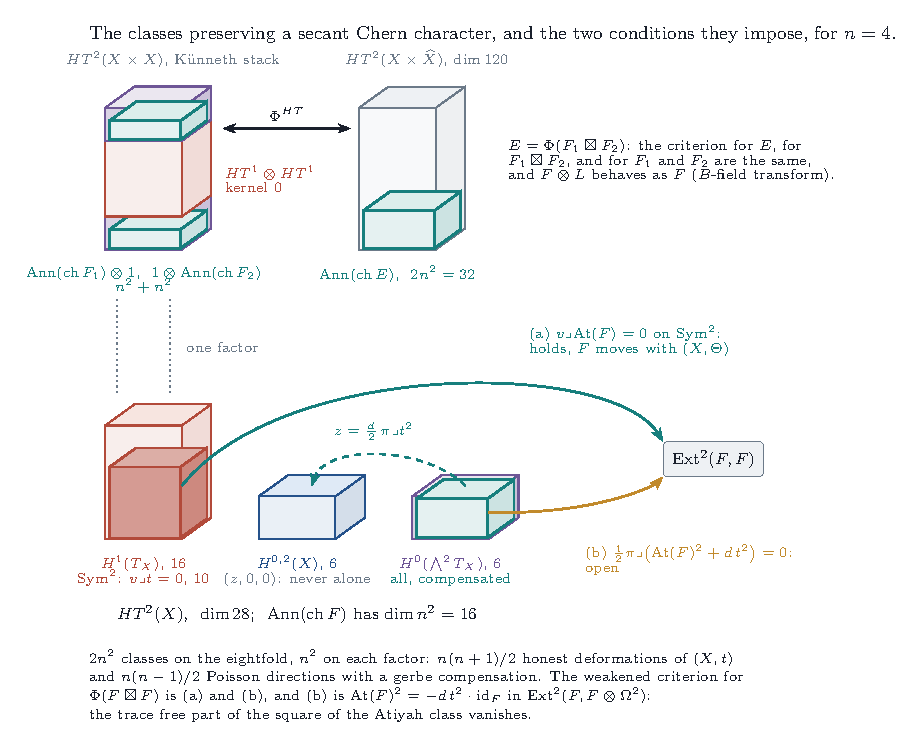
\includegraphics[width=\textwidth]{fig_factor}
\caption{\Cref{thm:factor} for $n=4$. Top: the K\"unneth stack of
$HT^{2}(X\times X)$, whose middle summand $HT^{1}\otimes HT^{1}$ meets the
kernel in zero by (i), so that the classes preserving $\ch(F_{1}\boxtimes F_{2})$
are two copies of the kernel on one factor; across Orlov's isomorphism,
$HT^{2}$ of the eightfold with the $2n^{2}$ classes preserving $\ch(E)$.
Bottom: $HT^{2}(X)$ as three slabs with heights proportional to their
dimensions, and inside them the $n^{2}$ classes of \eqref{eq:secantkernel}:
the polarised deformations in front of $H^{1}(T_{X})$, and the whole of
$H^{0}(\bigwedge^{2}T_{X})$, each bivector tilted into $H^{0,2}$ by its
compensation $\tfrac d2\,\pi\lrcorner t^{2}$; nothing in $H^{0,2}$ alone
preserves $\ch(F)$. On the right, the two conditions that the evaluation map
imposes on the two parts, (a) closed by the construction of $\cF$ and (b)
the identity \eqref{eq:heisenberg}.}
\label{fig:factor}
\end{figure}

\begin{corollary}[The remaining condition on the fourfold]\label{cor:markmancondition}
In \Cref{setup:markman} let $E=\Phi(\cF\boxtimes\cF)$. Then $E$ satisfies the
weakened criterion of \cite[Question 11.4]{Mar25b} if and only if
\begin{equation}\label{eq:heisenberg}
  \mathrm{At}(\cF)^{2}=-d\,\Theta^{2}\cdot\id_{\cF}
  \qquad\text{in }\Ext^{2}(\cF,\cF\otimes\Omega^{2}_{X}).
\end{equation}
Equivalently, writing $\mathrm{At}(\cF)=\sum_{a}A_{a}\otimes p_{a}$ with
$A_{a}\in\Ext^{1}(\cF,\cF)$ in a basis $p_{a}$ of $H^{1,0}(X)$, and
$\Theta=\sum_{a}p_{a}\wedge q_{a}$ with $q_{a}\in H^{0,1}(X)$, all the
commutators $A_{a}A_{b}-A_{b}A_{a}\in\Ext^{2}(\cF,\cF)$ are the scalars
$\pm2d\,(q_{a}\wedge q_{b})\cdot\id_{\cF}$ prescribed by $\Theta^{2}$, the
sign being fixed by the Koszul rule.
\end{corollary}

\begin{proof}
By \Cref{prop:markman8}(iii), $\ch(\cF)=u_{\Theta}+3v_{\Theta}$, so
\Cref{thm:factor} applies with $n=4$, $(a,b)=(1,3)$ and $F_{1}=F_{2}=\cF$, and
$E$ satisfies the criterion if and only if $\cF$ satisfies (a) and (b). It
remains to show that (a) holds. The data of \Cref{setup:markman} are a
principally polarised fourfold $(X,\Theta)$ and $N$ points $x_{i}\in X$ with
$D_{i}=\tau_{x_{i}}^{*}\Theta$. The conditions imposed on the $D_{i}$, that
the intersections of two, three and four of them be smooth of the expected
codimension and that five of them be disjoint, are open in the parameter
space of such data over the local universal deformation $S$ of $(X,\Theta)$,
by the openness of smoothness for a proper flat family and the properness of
the projection. The isolated points of $Z$, being transversal intersections
of four divisors, form a finite \'etale cover of the open set where the
conditions hold, so the $m$ points to be normalised can be followed locally;
the partial normalisation separates two smooth branches at each of them and
commutes with base change. The construction therefore produces a perfect
complex $\cF_{S}$ on the universal family over a neighbourhood of the base
point in $S$, whose fibre at the base point is $\cF$ and whose base has
Kodaira--Spencer image the whole space of polarised deformations, of
dimension $10=n(n+1)/2$. The obstruction $v\lrcorner\,\mathrm{At}(\cF)$ to
extending $\cF$ along $v$ vanishes for every $v$ along which $\cF$ extends
\cite{Tod09}, and this is (a).

For the reformulation, $\Omega^{1}_{X}=\cO_{X}\otimes H^{1,0}$ gives
$\mathrm{At}(\cF)=\sum_{a}A_{a}\otimes p_{a}$, and
$\mathrm{At}(\cF)^{2}=-\sum_{a<b}(A_{a}A_{b}-A_{b}A_{a})\otimes p_{a}\wedge p_{b}$
by the Koszul rule, while $\Theta^{2}=-2\sum_{a<b}(p_{a}\wedge p_{b})(q_{a}\wedge q_{b})$
for $\Theta=\sum_{a}p_{a}\wedge q_{a}$. Comparing coefficients of
$p_{a}\wedge p_{b}$ gives the commutator relations.
\end{proof}

\begin{remark}[Scope of the reduction]\label{rem:factorclosed}
The reduction accomplishes three things. First, it removes the eightfold:
the condition of \Cref{rem:onecondition}, on an object of rank $8d(d-9)$ on
$X\times\widehat X$ of Weil type, is equivalent to one identity
\eqref{eq:heisenberg} for a rank one complex on the fourfold, in the Yoneda
algebra $\Ext^{*}(\cF,\cF)$. The dimension of the space of classes that has
to be killed drops from $2n^{2}$ to $n^{2}$ and, by (a), to $n(n-1)/2=6$. At
$n=3$ the count $n^{2}=9$ is the nine-dimensional kernel of
\cite[Corollaries 8.3.12 and 8.5.2]{Mar25a}, which \eqref{eq:secantkernel}
writes out for every secant object in every dimension. Second, the half of
that space made of geometric deformations imposes nothing, because Markman's
construction is uniform over the moduli of principally polarised fourfolds.
Third, by \Cref{lem:bfield} the two forms of the criterion, for $E$ with
$\ch(E)$ and for the twisted object with $\kappa(E)$, coincide, so nothing
is lost by working with the untwisted object.

What remains is the identity itself, which is a Heisenberg relation: the
components of the Atiyah class in the $n$ tangent directions must commute up
to the scalars prescribed by $\Theta^{2}$, and the Chern character forces
only the trace of the relation. The identity says exactly that $\cF$
deforms, as an object of the deformed category, along the Poisson directions
of $X$ compensated by the gerbe classes $\tfrac d2\,\pi\lrcorner\,\Theta^{2}$;
these are the noncommutative first order deformations of $X$ with a gerby
correction, in the language of \cite[Section 8.5]{Mar25a}. It holds in the
one case where the method is known to work. For Markman's sheaves
$\cF_{1}=I_{\bigcup C_{i}}(\Theta)$ on the Jacobian threefold of
\cite[Section 11.1]{Mar25b}, with $\ch=u_{\Theta}+v_{\Theta}$ and $d=q$, the
kernel of the obstruction map equals the annihilator of the Chern character
\cite[Corollary 8.3.12]{Mar25a}, which is stronger than the weakened
criterion; so by \Cref{thm:factor}(iii) these sheaves satisfy
$\mathrm{At}(\cF_{1})^{2}=-q\,\Theta^{2}\cdot\id$ on the threefold. For the
rank one complex of \Cref{setup:markman} on the fourfold, the identity is a
computation of Yoneda products in $\Ext^{*}(\cF,\cF)$, and the computation
can be made local. Below we carry it out at one point of the support and
find that the identity fails.
\end{remark}

\subsubsection*{Failure at an isolated double point}

The identity \eqref{eq:heisenberg} can be tested locally. The evaluation map
is an algebra homomorphism \cite[(8.3.3)]{Mar25a}, so on a bivector
$\theta\wedge\theta'$ it is the Yoneda product of the classes
\[
  A_{\theta}=\operatorname{ev}_{\cF}(\theta)=\theta\lrcorner\,\mathrm{At}(\cF)
  \in\Ext^{1}(\cF,\cF),\qquad\theta\in H^{0}(T_{X}),
\]
which are the first order deformations of $\cF$ along the translations of
$X$. The product of two global classes restricts to the product of their
germs. At a point where the support of $\cF$ has two smooth branches of
codimension two meeting transversally, the germs multiply nontrivially;
since the compensating classes $z\cdot\id_{\cF}$ have zero germs, the
identity fails. Markman's construction has such points and cannot avoid
them.

\begin{lemma}[Localisation]\label{lem:edge}
Let $F$ be a perfect complex on a smooth projective variety $Y$, let
$\cE xt^{m}(F,F)$ be the sheaf associated with $U\mapsto\Hom_{D(U)}(F|_{U},F|_{U}[m])$,
and let $e\colon\Ext^{m}(F,F)\to H^{0}(Y,\cE xt^{m}(F,F))$ send a morphism
$F\to F[m]$ to its germs. Then $e$ is compatible with Yoneda products;
$e(z\cdot\id_{F})=0$ for $z\in H^{m}(\cO_{Y})$, $m\ge1$; and for
$\theta\in H^{0}(T_{Y})$ the germ of $A_{\theta}$ at $p$ is the class of the
jet extension $0\to F_{p}\to J_{\theta}(F_{p})\to F_{p}\to0$ of the germ
$F_{p}$ along the derivation $\theta$ of $\cO_{Y,p}$, which is
$\cO_{Y,p}$-linear in $\theta$.
\end{lemma}

\begin{proof}
Composition of morphisms commutes with restriction to open sets; this is the
first assertion. For the second, $z\cdot\id_{F}$ restricted to an affine open
$U$ is $z|_{U}\cdot\id_{F|_{U}}$, and $z|_{U}\in H^{m}(U,\cO_{U})=0$. For the
third, the Atiyah class of $F$ is the class of the first jet sequence
$0\to F\otimes\Omega^{1}_{Y}\to J^{1}(F)\to F\to0$ \cite[Section 3]{BF03},
and its restriction to $U$ is the jet sequence of $F|_{U}$. Contracting with
$\theta$ is pushing out along $\id\otimes\theta\colon F\otimes\Omega^{1}\to F$,
which produces the extension $J_{\theta}(F)$ whose underlying sheaf is
$F\oplus F$ with $f\cdot(s,s')=(fs+\theta(f)s',fs')$. Linearity in $\theta$
is linearity of the contraction.
\end{proof}

\begin{lemma}[Two branches through a point]\label{lem:localproducts}
Let $\cO$ be the local ring of $\CC^{4}$ at the origin or its completion
$\CC[[x_{1},\dots,x_{4}]]$; let $P_{1}=\{x_{1}=x_{2}=0\}$ and
$P_{2}=\{x_{3}=x_{4}=0\}$, two smooth surfaces meeting transversally at the
origin; put $N_{1}=\langle\partial_{1},\partial_{2}\rangle$ and
$N_{2}=\langle\partial_{3},\partial_{4}\rangle$, the normal spaces of $P_{1}$
and of $P_{2}$ at the origin, so that
$\bigwedge^{2}T_{0}=\bigwedge^{2}N_{1}\oplus N_{1}\otimes N_{2}\oplus\bigwedge^{2}N_{2}$.
For a germ of vector field $\theta$ and a perfect complex $F$ of
$\cO$-modules write $a_{\theta}\in\Ext^{1}_{\cO}(F,F)$ for the class of the
jet extension along $\theta$.
\begin{enumerate}[label=\textup{(\roman*)},nosep]
\item For $F=I=I_{P_{1}}\cap I_{P_{2}}$, the ideal of the union,
  $\Ext^{2}_{\cO}(I,I)\cong N_{1}\otimes N_{2}$, a vector space of dimension
  four on which the maximal ideal acts trivially, and
  $a_{\theta}a_{\theta'}$ is, up to a fixed nonzero scalar, the component of
  $\theta(0)\wedge\theta'(0)$ in $N_{1}\otimes N_{2}$. In particular
  $a_{\theta}a_{\theta'}\ne0$ unless $\theta(0)\wedge\theta'(0)\in
  \bigwedge^{2}N_{1}\oplus\bigwedge^{2}N_{2}$.
\item For $F=K=[\cO\to\cO_{P_{1}}\oplus\cO_{P_{2}}]$, the complex in degrees
  $0$ and $1$ whose cohomology is $I$ in degree $0$ and the residue field $k$
  in degree $1$, $a_{\theta}a_{\theta'}\ne0$ unless
  $\theta(0)\wedge\theta'(0)\in N_{1}\otimes N_{2}$.
\end{enumerate}
In both cases the bilinear map $(\theta,\theta')\mapsto a_{\theta}a_{\theta'}$
is nonzero, and it depends only on $\theta(0)\wedge\theta'(0)$.
\end{lemma}

\begin{proof}
Write $A=\CC[x_{1},x_{2}]$, $B=\CC[x_{3},x_{4}]$, $R=A\otimes_{\CC}B$, with
maximal ideals $\mathfrak m_{A}$, $\mathfrak m_{B}$ at the origin, and
$k=\CC$. The ideal of the union is $I=\mathfrak m_{A}R\cap\mathfrak m_{B}R
=\mathfrak m_{A}\otimes_{\CC}\mathfrak m_{B}$, because the two ideals are
generated by disjoint sets of variables. Everything below is homogeneous, the
$\Ext$ groups in degree two are of finite length, and finite length modules
and jet classes are unchanged by the flat base change from $R$ to $\cO$; so we
compute over $R$. For finitely generated modules $M,M'$ over $A$ and $N,N'$
over $B$, the tensor product of free resolutions resolves $M\otimes_{\CC}N$
and the K\"unneth formula gives
\begin{equation}\label{eq:kunnethext}
  \Ext^{n}_{R}(M\otimes N,M'\otimes N')
  =\bigoplus_{i+j=n}\Ext^{i}_{A}(M,M')\otimes_{\CC}\Ext^{j}_{B}(N,N'),
\end{equation}
compatibly with Yoneda products up to the Koszul sign, since a product of
chain maps on the tensor product of resolutions is the tensor product of the
products.

The basic case is a single plane. The Koszul complex
$0\to A\xrightarrow{(-x_{2},x_{1})^{t}}A^{2}\xrightarrow{(x_{1},x_{2})}\mathfrak m_{A}\to0$
is a free resolution, so $\mathfrak m_{A}$ has projective dimension one and
$\Ext^{i}_{A}(\mathfrak m_{A},-)=0$ for $i\ge2$; and
$\Ext^{1}_{A}(\mathfrak m_{A},\mathfrak m_{A})=\coker\bigl(\Hom(A^{2},\mathfrak m_{A})
\to\Hom(A,\mathfrak m_{A})\bigr)=\mathfrak m_{A}/\mathfrak m_{A}^{2}$, a
two-dimensional space killed by $\mathfrak m_{A}$. On a complex of free
modules with differential $d$ the jet extension along a derivation $D$ is the
complex with terms $P_{i}\oplus P_{i}$ and differential
$\bigl(\begin{smallmatrix}d&-D(d)\\0&d\end{smallmatrix}\bigr)$, $D(d)$ the
entrywise derivative, because the twisted module $J_{D}(P_{i})$ is free on the
elements $(e,0)$ and $(0,e)$ and $d(0,e)=\sum_{l}d_{le}(0,e_{l})-\sum_{l}D(d_{le})(e_{l},0)$;
so the jet class is represented by the degree $-1$ chain map $-D(d)$. For
$D=\partial_{i}$ on the Koszul complex this is $e\mapsto\delta_{i2}f_{1}-\delta_{i1}f_{2}$
on the generator $e$ of the last term, whose image in
$\mathfrak m_{A}/\mathfrak m_{A}^{2}$ is $\delta_{i2}x_{1}-\delta_{i1}x_{2}$:
\[
  \alpha_{1}:=a_{\partial_{1}}=-[x_{2}],\qquad
  \alpha_{2}:=a_{\partial_{2}}=[x_{1}],
\]
a basis of $\Ext^{1}_{A}(\mathfrak m_{A},\mathfrak m_{A})$, which we identify
with $N_{1}$ by $\partial_{i}\mapsto\alpha_{i}$. Similarly $\beta_{3},\beta_{4}$
form a basis of $\Ext^{1}_{B}(\mathfrak m_{B},\mathfrak m_{B})$, identified
with $N_{2}$.

(i) By \eqref{eq:kunnethext} with $M=M'=\mathfrak m_{A}$, $N=N'=\mathfrak m_{B}$,
\[
  \Ext^{2}_{R}(I,I)=\Ext^{1}_{A}\otimes\Ext^{1}_{B}=N_{1}\otimes N_{2},
\]
the other two summands vanishing by the projective dimension, and it is killed
by $\mathfrak m_{A}$ and $\mathfrak m_{B}$. The derivation $\partial_{1}$ acts on
the factor $A$, so the jet extension of $I=\mathfrak m_{A}\otimes\mathfrak m_{B}$
along it is $J_{\partial_{1}}(\mathfrak m_{A})\otimes\mathfrak m_{B}$ and
$a_{\partial_{1}}=\alpha_{1}\otimes1$; likewise $a_{\partial_{2}}=\alpha_{2}\otimes1$,
$a_{\partial_{3}}=1\otimes\beta_{3}$, $a_{\partial_{4}}=1\otimes\beta_{4}$.
Hence $a_{\partial_{i}}a_{\partial_{j}}=\pm\alpha_{i}\otimes\beta_{j}$ for
$i\le2<j$, the four of them a basis of $N_{1}\otimes N_{2}$, while
$a_{\partial_{1}}a_{\partial_{2}}=\alpha_{1}\alpha_{2}\otimes1=0$ and
$a_{\partial_{3}}a_{\partial_{4}}=0$ because $\Ext^{2}_{A}(\mathfrak m_{A},\mathfrak m_{A})=0$.
For germs $\theta=\sum_{i}c^{i}\partial_{i}$ and $\theta'=\sum_{j}c'^{j}\partial_{j}$
the linearity of \Cref{lem:edge} and the triviality of the module structure
give $a_{\theta}a_{\theta'}=\sum_{i,j}c^{i}(0)c'^{j}(0)\,a_{\partial_{i}}a_{\partial_{j}}$,
the image of $\theta(0)\wedge\theta'(0)$ under the projection of
$\bigwedge^{2}T_{0}$ onto $N_{1}\otimes N_{2}$ followed by the isomorphism
$\partial_{i}\otimes\partial_{j}\mapsto\pm\alpha_{i}\otimes\beta_{j}$.

(ii) Let $Q=\cO_{P_{1}}\oplus\cO_{P_{2}}$. The map $\cO\to Q$ has kernel $I$
and cokernel $\cO/(I_{P_{1}}+I_{P_{2}})=k$, so $K$ sits in an exact triangle
$I\xrightarrow{\iota}K\xrightarrow{\pi}k[-1]\xrightarrow{\varepsilon}I[1]$.
The jet extension along $\theta$ is an exact functor, natural in its
argument, so the jet classes commute with $\iota$ and $\pi$; and for the
residue field $a^{k}_{\theta}$ depends only on $\theta(0)$, because
$\Ext^{1}(k,k)$ is killed by $\mathfrak m$ and the class is linear in
$\theta$. Therefore
\[
  \pi[2]\circ a^{K}_{\theta}a^{K}_{\theta'}
  =a^{k}_{\theta}a^{k}_{\theta'}\circ\pi
  =\pi^{*}\bigl(a^{k}_{\theta(0)}a^{k}_{\theta'(0)}\bigr),
  \qquad\pi^{*}\colon\Ext^{2}(k,k)\to\Ext^{1}(K,k),
\]
and it suffices to show that the right hand side is nonzero. The long exact
sequence of the triangle for $\Hom(-,k)$ reads
\[
  \Hom(I,k)\xrightarrow{\;\varepsilon^{*}\;}\Ext^{2}(k,k)\xrightarrow{\;\pi^{*}\;}
  \Ext^{1}(K,k),
\]
so $\ker\pi^{*}=\image\varepsilon^{*}$. Now $k=k_{A}\otimes k_{B}$ and, by
\eqref{eq:kunnethext}, $\Ext^{*}(k,k)$ is the tensor product of
$\Ext^{*}_{A}(k,k)$ and $\Ext^{*}_{B}(k,k)$. On the Koszul resolution
$A\to A^{2}\to A$ of $k_{A}$ the jet chain maps of $\partial_{1},\partial_{2}$
are $-D(d)$ as above, and their composite $A\to A$ is the scalar $-1$, whose
class in $\Ext^{2}_{A}(k,k)=\Hom(A,k)=k$ is nonzero; the degree one classes
$\gamma_{1},\gamma_{2}$ of $\partial_{1},\partial_{2}$ are the basis
$-e_{1}^{*},-e_{2}^{*}$ of $\Ext^{1}_{A}(k,k)=\Hom(A^{2},k)$, and their
product spans $\Ext^{2}_{A}(k,k)$. With the analogous classes
$\gamma_{3},\gamma_{4}$ over $B$, the products $\gamma_{1}\gamma_{2}\otimes1$,
$\gamma_{i}\otimes\gamma_{j}$ ($i\le2<j$) and $1\otimes\gamma_{3}\gamma_{4}$
form a basis of $\Ext^{2}(k,k)=k\oplus(k^{2}\otimes k^{2})\oplus k$, so
$\partial_{i}\wedge\partial_{j}\mapsto a^{k}_{\partial_{i}}a^{k}_{\partial_{j}}$
identifies $\bigwedge^{2}(N_{1}\oplus N_{2})$ with $\Ext^{2}(k,k)$, and
$a^{k}_{\theta(0)}a^{k}_{\theta'(0)}$ is the image of $\theta(0)\wedge\theta'(0)$. The
class $\varepsilon$ is the K\"unneth product $\varepsilon_{A}\otimes\varepsilon_{B}$
of the classes of $0\to\mathfrak m_{A}\to A\to k\to0$ and its $B$-analogue,
because $K$ is the two-step truncation of the tensor product of the complexes
$[A\to k_{A}]$ and $[B\to k_{B}]$ and $\varepsilon$ is the inclusion of the
omitted term $k_{A}\otimes k_{B}$. Hence $\varepsilon^{*}$ maps
$\Hom(I,k)=\Hom(\mathfrak m_{A},k)\otimes\Hom(\mathfrak m_{B},k)$ into
$\Ext^{1}_{A}(k,k)\otimes\Ext^{1}_{B}(k,k)=N_{1}\otimes N_{2}$, and onto it,
since $\Hom(\mathfrak m_{A},k)\to\Ext^{1}_{A}(k,k)$ is an isomorphism: it is
the connecting homomorphism of the sequence, injective because
$\Hom(A,k)\to\Hom(\mathfrak m_{A},k)$ is zero and surjective because
$\Ext^{1}_{A}(A,k)=0$. So $\ker\pi^{*}=N_{1}\otimes N_{2}$
and $\pi^{*}(\theta(0)\wedge\theta'(0))\ne0$ exactly when
$\theta(0)\wedge\theta'(0)\notin N_{1}\otimes N_{2}$.
\end{proof}

\begin{theorem}[Markman's candidate does not satisfy the weakened criterion]
\label{thm:candidatefails}
In \Cref{setup:markman}, for every odd squarefree $d\ge3$, every choice of the
translates $D_{i}$ in general position and every choice of the $m$ points to
be normalised:
\begin{enumerate}[label=\textup{(\roman*)},nosep]
\item the identity \eqref{eq:heisenberg} fails: there is a constant bivector
  $\pi\in H^{0}(\bigwedge^{2}T_{X})$ with
  $\tfrac12\pi\lrcorner\bigl(\mathrm{At}(\cF)^{2}+d\,\Theta^{2}\cdot\id_{\cF}\bigr)\ne0$
  in $\Ext^{2}(\cF,\cF)$;
\item $\cF$ does not satisfy the weakened criterion: the class
  $x_{\cF}=(\tfrac d2\,\pi\lrcorner\,\Theta^{2},0,\pi)$ has
  $x_{\cF}\lrcorner\,\ch(\cF)=0$ and $\operatorname{ev}_{\cF}(x_{\cF})\ne0$;
\item for every perfect complex $F_{2}$ on $X$ with Chern character on the
  secant plane, in particular for $F_{2}=\cF$ and $F_{2}=\cF^{\vee}$, the
  object $E=\Phi(\cF\boxtimes F_{2})$ on the eightfold $X\times\widehat X$ of
  Weil type does not satisfy the weakened criterion of
  \cite[Question 11.4]{Mar25b}: the class $x=\Phi^{HT}(x_{\cF}\otimes1)$
  satisfies $x\lrcorner\,\ch(E)=0$ and $\operatorname{ev}_{E}(x)\ne0$, so
  $\sigma_{E}$ is not injective on the image of $\operatorname{ev}_{E}$.
\end{enumerate}
\end{theorem}

\begin{proof}
(i) The surfaces $Z_{i}$ and $Z_{j}$ at cyclic distance at least three meet
in the $24$ points of $D_{i}\cap D_{i+1}\cap D_{j}\cap D_{j+1}$, and there are
$12N(N-5)=(d+9)(3d-3)$ such points, of which $m=(d+9)(2d-1)$ are normalised;
the remaining $(d+9)(d-2)\ge12$ are not. Let $p$ be one of the latter. The
four divisors through $p$ meet transversally, so their local equations
$x_{1},\dots,x_{4}$ form a regular system of parameters of $\cO_{X,p}$ and
identify its completion with $\CC[[x_{1},\dots,x_{4}]]$, with
$D_{i}=\{x_{1}=0\}$, $D_{i+1}=\{x_{2}=0\}$, $D_{j}=\{x_{3}=0\}$ and
$D_{j+1}=\{x_{4}=0\}$; hence $Z_{i}=P_{1}$ and $Z_{j}=P_{2}$ in the
notation of \Cref{lem:localproducts}. The completion is flat, so a class
whose completed germ is nonzero is nonzero. No other $D_{k}$ passes through
$p$, since five divisors have empty intersection, so no other component of
$Z$ does. Near $p$ the map $\nu$ is an isomorphism,
$\nu_{*}\cO_{\widetilde Z}=\cO_{Z}$, and $\cF$ is the ideal sheaf
$I_{Z}=I_{P_{1}}\cap I_{P_{2}}$ twisted by the locally trivial $\cO_{X}(3\Theta)$:
the germ $\cF_{p}$ is the module $I$ of \Cref{lem:localproducts}(i).

Let $\theta,\theta'\in H^{0}(T_{X})$ be constant vector fields whose values
at $p$ are $\partial_{1}$ and $\partial_{3}$; they exist because the constant
fields span every tangent space. Put $\pi=\theta\wedge\theta'$. Since
$\operatorname{ev}_{\cF}$ is an algebra homomorphism,
$\operatorname{ev}_{\cF}(\pi)=\tfrac12\pi\lrcorner\,\mathrm{At}(\cF)^{2}
=A_{\theta}A_{\theta'}$. By \Cref{lem:edge} its germ at $p$ is
$a_{\theta}a_{\theta'}$, which is nonzero by \Cref{lem:localproducts}(i),
because $\partial_{1}\wedge\partial_{3}$ has nonzero component in
$N_{1}\otimes N_{2}$. The germ of
$\tfrac d2(\pi\lrcorner\,\Theta^{2})\cdot\id_{\cF}$ at $p$ is zero by
\Cref{lem:edge}. So the germ at $p$ of
$\tfrac12\pi\lrcorner(\mathrm{At}(\cF)^{2}+d\Theta^{2}\cdot\id_{\cF})$ is
$a_{\theta}a_{\theta'}\ne0$, and the class itself is nonzero.

(ii) By \Cref{thm:factor}(ii) the class $x_{\cF}$ preserves $\ch(\cF)$, and by
\eqref{eq:evgeneral} $\operatorname{ev}_{\cF}(x_{\cF})$ is the class of (i).

(iii) Both $\cF$ and $\cF^{\vee}$ are admissible as $F_{2}$, since
$\ch(\cF^{\vee})=u_{\Theta}-3v_{\Theta}$ lies on the secant plane. By
\Cref{thm:factor}(iv), $E$ satisfies the criterion only if both factors do,
and $\cF$ does not. The class $x$ of the statement is the transport of
$x_{\cF}\otimes1\in\Ann_{HT^{2}}(\ch(\cF\boxtimes F_{2}))$, on which
$\operatorname{ev}$ is $\pm\operatorname{ev}_{\cF}(x_{\cF})\otimes\id_{F_{2}}\ne0$;
since $\Phi$ is an isomorphism on $\Ext^{2}$, $\operatorname{ev}_{E}(x)\ne0$.
The last assertion follows from the commutative square of
\Cref{setup:criterion}: $\sigma_{E}(\operatorname{ev}_{E}(x))=x\lrcorner\,\ch(E)=0$
with $\operatorname{ev}_{E}(x)\ne0$.
\end{proof}

\Cref{fig:doublepoint} draws the local computation at the double point.

\begin{remark}[Normalised points]\label{rem:normalisedpoints}
At a normalised point the germ of $\cF$ is the complex $K$ of
\Cref{lem:localproducts}(ii), and the same argument, with
$\theta(p)=\partial_{1}$ and $\theta'(p)=\partial_{2}$, produces a nonzero
germ. The failure therefore does not depend on which points are separated.
Separating all of them would not help even if the construction allowed it:
normalising every isolated point changes $\chi(\cO_{\widetilde Z})$ to
$110N-12N^{2}+12N(N-5)=50N$, while the secant plane requires
$(d+9)(27-d)=72N-4N^{2}$, and the two agree only for $N=11/2$. The two local
computations are complementary: at a point of type (i) the obstruction lies
in $N_{1}\otimes N_{2}$, at a point of type (ii) in
$\bigwedge^{2}N_{1}\oplus\bigwedge^{2}N_{2}$, and together these exhaust
$\bigwedge^{2}T_{p}$.
\end{remark}

\begin{figure}[tbp]
\centering
  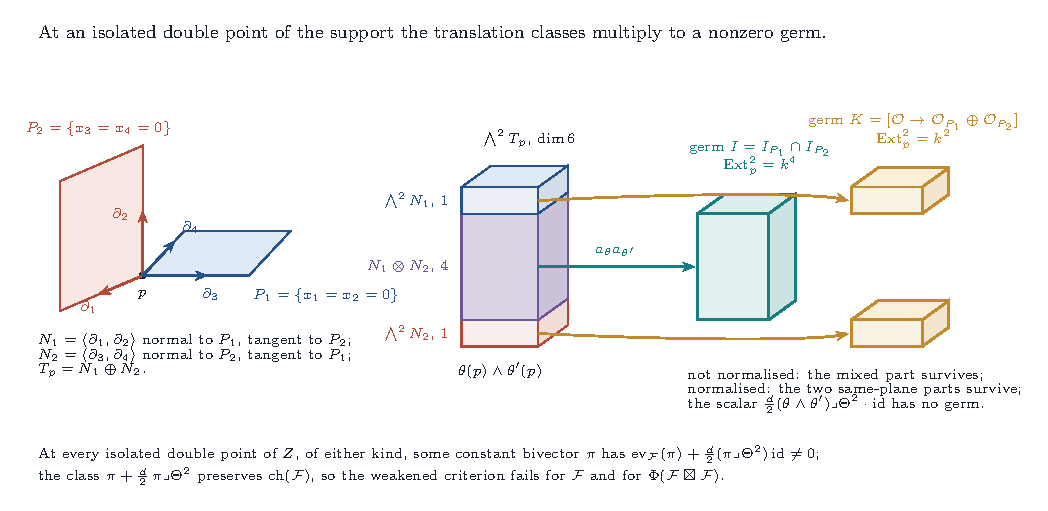
\includegraphics[width=\textwidth]{fig_doublepoint}
\caption{\Cref{lem:localproducts} and \Cref{thm:candidatefails}. Left: two
smooth surfaces of a fourfold meeting transversally at $p$, with the normal
spaces $N_{1}$ and $N_{2}$, each tangent to the other branch. Centre: the
bivectors at $p$, split into $\bigwedge^{2}N_{1}$, $N_{1}\otimes N_{2}$ and
$\bigwedge^{2}N_{2}$, with heights proportional to the dimensions. Right: the
local $\Ext^{2}$ of the germ of $\cF$ at $p$ in the two cases, and the part
of the bivectors that the products of the translation classes carry onto it:
the mixed part when the point is not normalised, the two same-plane parts
when it is. The compensating scalar has no germ, so in either case the
identity \eqref{eq:heisenberg} fails at $p$.}
\label{fig:doublepoint}
\end{figure}

\begin{corollary}[A local obstruction in every dimension]\label{cor:localobstruction}
Let $(X,t)$ be a polarised abelian variety of dimension $n\ge4$ and $F$ a
perfect complex on $X$ with $\ch(F)=au_{t}+bv_{t}$, $(a,b)\ne(0,0)$. Suppose
that at some point $p$ the germ $F_{p}$ is isomorphic, in the derived
category of $\cO_{X,p}$-modules, to the ideal of the union of two smooth germs
of codimension two meeting transversally along a germ of codimension four,
or, when $n=4$, to the complex $[\cO\to\cO_{P_{1}}\oplus\cO_{P_{2}}]$ of two
such germs. Then $F$ does not satisfy the weakened criterion, and neither does
$\Phi(F\boxtimes F_{2})$ on $X\times\widehat X$ for any secant $F_{2}$. In
particular, in every dimension $n\ge4$, the union $Z$ of the intersections
$D_{i}\cap D_{i+1}$ of consecutive translates of a polarisation in general
position contains, for every pair $(i,j)$ of nonconsecutive indices, a
subvariety $Z_{i}\cap Z_{j}$ of codimension four along which $Z$ has two
transversal branches; any secant object of the form $[\cO_{X}\to\nu_{*}\cO_{\widetilde Z}]\otimes L$
in which $\nu$ is an isomorphism at a general point of one such
$Z_{i}\cap Z_{j}$ fails the criterion.
\end{corollary}

\begin{proof}
In formal coordinates $x_{1},\dots,x_{n}$ at $p$ with the two branches
$\{x_{1}=x_{2}=0\}$ and $\{x_{3}=x_{4}=0\}$, which exist because the four
local equations of the branches form part of a regular system of
parameters, the ideal is
$I\otimes_{\CC}\CC[x_{5},\dots,x_{n}]$ with $I$ as in \Cref{lem:localproducts},
and \eqref{eq:kunnethext} with the third factor gives
$\Ext^{2}(I_{p},I_{p})=N_{1}\otimes N_{2}\otimes\cO_{W,p}$, where $W$ is the
intersection of the branches. The jet classes along $\partial_{5},\dots,\partial_{n}$
vanish, since these derivations act on a free factor, and the products of the
classes along $\partial_{1},\dots,\partial_{4}$ are as in the lemma. Reducing
modulo the maximal ideal of $\cO_{W,p}$ shows that $a_{\theta}a_{\theta'}\ne0$
whenever $\theta(p)\wedge\theta'(p)$ has a nonzero component in
$N_{1}\otimes N_{2}$. When $n=4$ and $F_{p}$ is the complex
$[\cO\to\cO_{P_{1}}\oplus\cO_{P_{2}}]$, \Cref{lem:localproducts}(ii) applies
directly. The rest of the argument is that of
\Cref{thm:candidatefails}, using \Cref{thm:factor} for $n\ge3$. For the last
assertion, $Z_{i}\cap Z_{j}=D_{i}\cap D_{i+1}\cap D_{j}\cap D_{j+1}$ is a
transversal intersection of four divisors, of codimension four, and at a
general point of it no fifth divisor passes, so $Z$ has exactly the two
branches $Z_{i}$ and $Z_{j}$ there.
\end{proof}

\begin{remark}[Scope of the local obstruction]\label{rem:candidatemeaning}
\Cref{thm:candidatefails} answers the question posed in
\cite[Section 12]{Mar25b}: the secant objects proposed there do not satisfy
the weakened criterion of \cite[Question 11.4]{Mar25b}, for any
discriminant. The reason is local and geometric. That question asks whether
the semiregularity map may be required to be injective only on the image of
the evaluation map. For a secant object this image contains, by
\Cref{thm:factor}, the products $A_{\theta}A_{\theta'}$ of the translation
classes shifted by the scalars
$\tfrac d2(\theta\wedge\theta')\lrcorner\,\Theta^{2}$, and the
semiregularity map kills them all. For the criterion to hold these shifted
products must vanish, and they cannot: at an isolated double point of the
support, the translation classes of the two branches multiply to a nonzero
local class, while a scalar has no local class at all. The fourth ingredient
of \Cref{rem:deformation} can accordingly be stated more sharply. A secant
object of positive rank on a fourfold that satisfies the weakened criterion
must have, at every point, germs whose translation classes multiply to zero
in the local $\Ext^{2}$. By \Cref{lem:localproducts} this excludes every
support with two transversal branches of codimension two through a point,
whether or not the branches are separated, and by
\Cref{cor:localobstruction} it excludes the chain of consecutive
intersections of translates in every dimension. An object supported on a
smooth surface, or on surfaces meeting only along curves, is not excluded by
this argument, but no such object with Chern character on the secant plane
is known.
\end{remark}

\subsection{Smooth supports and four discriminants}
\label{ssec:smoothsupport}

\Cref{thm:candidatefails} and \Cref{cor:localobstruction} exclude every secant
object whose support has two transversal branches of codimension two
through a point. This leaves supports that are smooth or that meet
themselves only along curves, and \Cref{rem:candidatemeaning} ends with the
observation that no such object is known. In this subsection we explain why
the local argument cannot reach the smooth case, and then determine what a
smooth support can be. The answer is narrow: on the fourfold the invariants
of the support are forced, and the discriminant is confined to a finite list.

We begin with the fact that at a smooth point there is nothing local left to
compute.

\begin{proposition}[No local obstruction at a smooth point]\label{prop:smoothlocal}
Let $Y$ be a smooth variety with $\omega_{Y}\cong\cO_{Y}$ and let $S\subset Y$
be smooth of codimension two. Then
\[
  \cE xt^{0}(\cI_{S},\cI_{S})=\cO_{Y},\qquad
  \cE xt^{1}(\cI_{S},\cI_{S})=N_{S/Y},\qquad
  \cE xt^{q}(\cI_{S},\cI_{S})=0\quad(q\ge2),
\]
and the same holds for $\cI_{S}\otimes L$ for any line bundle $L$.
Consequently, for $F=\cI_{S}\otimes L$ both sides of \eqref{eq:heisenberg}
have vanishing germs in $\cE xt^{2}$, and \Cref{lem:edge} decides nothing.
\end{proposition}

\begin{proof}
Twisting by $L$ changes neither side, so take $F=\cI_{S}$. The sheaf
$\cI_{S}$ is torsion free of rank one, and its dual is $\cO_{Y}$ because $S$
has codimension two; hence every local endomorphism of $\cI_{S}$ is
multiplication by a function, and
$\cE xt^{0}(\cI_{S},\cI_{S})=\cO_{Y}$. Apply $\cH om(-,\cI_{S})$ to
\begin{equation}\label{eq:idealseq}
  0\to\cI_{S}\to\cO_{Y}\to\cO_{S}\to0 .
\end{equation}
Since $\cE xt^{q}(\cO_{Y},\cI_{S})=0$ for $q\ge1$, the long exact sequence
gives
\begin{equation}\label{eq:shift}
  \cE xt^{q}(\cI_{S},\cI_{S})\cong\cE xt^{q+1}(\cO_{S},\cI_{S})
  \qquad(q\ge1).
\end{equation}
Now apply $\cH om(\cO_{S},-)$ to \eqref{eq:idealseq}. Because $S$ is smooth of
codimension two, hence a local complete intersection, the Koszul resolution
gives $\cE xt^{k}(\cO_{S},\cO_{Y})=0$ for $k\ne2$ and
$\cE xt^{2}(\cO_{S},\cO_{Y})=\omega_{S}\otimes\omega_{Y}^{-1}=\omega_{S}$,
while $\cE xt^{k}(\cO_{S},\cO_{S})=\bigwedge^{k}N_{S/Y}$ for $0\le k\le2$ and
zero otherwise. Computing both from the same Koszul complex shows that the
map
\[
  \rho\colon\cE xt^{2}(\cO_{S},\cO_{Y})=\omega_{S}
  \longrightarrow
  \cE xt^{2}(\cO_{S},\cO_{S})=\textstyle\bigwedge^{2}N_{S/Y}=\omega_{S}
\]
induced by $\cO_{Y}\to\cO_{S}$ is the identity: in local coordinates in which
$S=\{x_{1}=x_{2}=0\}$, both groups are computed as $M/(x_{1},x_{2})M$ for
$M=\cO_{Y}$ and $M=\cO_{S}$, and the map is reduction modulo $(x_{1},x_{2})$,
which is the identity on $\cO_{S}$.

Consider the long exact sequence of $\cH om(\cO_{S},-)$ in degrees two and
three. Since $\rho$ is surjective and $\cE xt^{3}(\cO_{S},\cO_{Y})=0$, the
segment
\[
  \cE xt^{2}(\cO_{S},\cO_{Y})\xrightarrow{\ \rho\ }
  \cE xt^{2}(\cO_{S},\cO_{S})\to
  \cE xt^{3}(\cO_{S},\cI_{S})\to
  \cE xt^{3}(\cO_{S},\cO_{Y})=0
\]
gives $\cE xt^{3}(\cO_{S},\cI_{S})=0$, so $\cE xt^{2}(\cI_{S},\cI_{S})=0$ by
\eqref{eq:shift}. For $k\ge3$ both $\cE xt^{k}(\cO_{S},\cO_{Y})$ and
$\cE xt^{k}(\cO_{S},\cO_{S})$ vanish, so
$\cE xt^{k+1}(\cO_{S},\cI_{S})=0$ and $\cE xt^{k}(\cI_{S},\cI_{S})=0$. In
degrees one and two, since $\rho$ is injective, the segment
\[
  0=\cE xt^{1}(\cO_{S},\cO_{Y})\to
  N_{S/Y}\to
  \cE xt^{2}(\cO_{S},\cI_{S})\to
  \cE xt^{2}(\cO_{S},\cO_{Y})\xrightarrow{\ \rho\ }
  \cE xt^{2}(\cO_{S},\cO_{S}),
\]
in which $N_{S/Y}=\cE xt^{1}(\cO_{S},\cO_{S})$, gives
$\cE xt^{2}(\cO_{S},\cI_{S})\cong N_{S/Y}$, and this is
$\cE xt^{1}(\cI_{S},\cI_{S})$ by \eqref{eq:shift}.

For the last assertion, the right side of \eqref{eq:heisenberg} has vanishing
germs by \Cref{lem:edge}, and the left side lies in
$\Ext^{2}(F,F\otimes\Omega^{2}_{Y})$, whose sheaf of germs in the
$\cE xt^{2}$ direction is $\cE xt^{2}(F,F)\otimes\Omega^{2}_{Y}=0$.
\end{proof}

\begin{remark}[The global form of the criterion]\label{rem:obstructionmoves}
\Cref{prop:smoothlocal} is the precise reason why the argument of
\Cref{thm:candidatefails} stops at a smooth support, and it also shows what
takes its place. Since $\cE xt^{2}=0$, the local-to-global spectral sequence
for $\Ext^{2}(\cI_{S},\cI_{S})$ has only two surviving rows,
$H^{1}(S,N_{S/Y})$ and $H^{2}(Y,\cO_{Y})$, and they sit in different steps of
the filtration: the first is the quotient that records the geometry of $S$,
the second the subgroup of scalars. A product $A_{\theta}A_{\theta'}$ of
translation classes therefore has a well defined image in $H^{1}(S,N_{S/Y})$,
while the scalar on the right of \eqref{eq:heisenberg} has image zero there.
The criterion thus splits into two conditions of different kinds: a vanishing
in $H^{1}(S,N_{S/Y})$, which is a statement about the normal bundle and not
about any point, and an identity in $H^{2}(Y,\cO_{Y})$. At a double point the
first condition already fails locally. At a smooth support it is a global
question, and what is decided here is which surfaces $S$ are available at
all.
\end{remark}

The invariants of a smooth support are far from free. Since the Todd class of
an abelian variety is trivial, Grothendieck--Riemann--Roch converts the Chern
character of the object into the complete set of numerical invariants of the
surface, and three classical inequalities then constrain them.

\begin{theorem}[The invariants of a smooth support]\label{thm:smoothinvariants}
Let $(X,\Theta)$ be a principally polarised abelian fourfold, let $d>0$, let
$b\in\ZZ_{>0}$, and let $\cF=\cI_{S}(b\Theta)$ be a coherent sheaf with
\[
  \ch(\cF)=u_{\Theta}+b\,v_{\Theta}
\]
and $S\subset X$ smooth. Write $N=\tfrac12\Nm_{K/\QQ}(b+\sqrt{-d})
=\tfrac12(b^{2}+d)$, $\iota\colon S\hookrightarrow X$ and
$\lambda=\iota^{*}\Theta$. Then $S$ is a surface and
\begin{equation}\label{eq:smoothinvariants}
\begin{aligned}
  [S]&=N\Theta^{2}, &\qquad \iota_{*}K_{S}&=\tfrac{4bN}{3}\,\Theta^{3},
  &\qquad \chi(\cO_{S})&=4N(2b^{2}-N),\\
  K_{S}^{2}&=12N(4b^{2}-N), &\qquad e(S)&=12N(4b^{2}-3N),
  &\qquad K_{S}\cdot\lambda&=32bN,
\end{aligned}
\end{equation}
with $\lambda^{2}=24N$ and $[S]^{2}=24N^{2}$. Moreover $K_{S}$ is globally
generated, hence nef; $S$ is minimal of general type; and
\begin{equation}\label{eq:threebounds}
  \tfrac{4}{9}b^{2}\ \le\ N\ \le\ b^{2},
  \qquad\text{equivalently}\qquad
  -\tfrac{1}{9}b^{2}\ \le\ d\ \le\ b^{2} .
\end{equation}
The lower bound is the Hodge index theorem and is implied by $d>0$; the upper
bound is the Bogomolov--Miyaoka--Yau inequality. In terms of $b$ and $d$ the
five invariants read
\begin{equation}\label{eq:bdform}
  \chi(\cO_{S})=(b^{2}+d)(3b^{2}-d),\quad
  K_{S}^{2}=3(b^{2}+d)(7b^{2}-d),\quad
  e(S)=3(b^{2}+d)(5b^{2}-3d),
\end{equation}
and the defect in the Bogomolov--Miyaoka--Yau inequality is
\begin{equation}\label{eq:bmydefect}
  3e(S)-K_{S}^{2}=24\,(b^{4}-d^{2}),
\end{equation}
so that the inequality amounts exactly to $d\le b^{2}$.
Finally, $K_{S}$ is never numerically proportional to $\lambda$.
\end{theorem}

\begin{proof}
Since $\ch_{0}(\cF)=1$ and $c_{1}(\cF)=b\Theta$, the sheaf
$\cF(-b\Theta)=\cI_{S}$ has $\ch_{0}=1$, $\ch_{1}=0$, so $S$ has codimension
at least two, and
\[
  \ch(\cO_{S})=1-\ch(\cI_{S})=1-\ch(\cF)\,e^{-b\Theta}.
\]
Put $z=b+\sqrt{-d}$, so that $z\bbar z=2N$. Since
$u_{\Theta}=\Re e^{\sqrt{-d}\Theta}$ and
$\sqrt d\,v_{\Theta}=\Im e^{\sqrt{-d}\Theta}$, we have
$\ch(\cF)=\Im\bigl(z\,e^{\sqrt{-d}\Theta}\bigr)/\sqrt d$, hence
$\ch(\cF)e^{-b\Theta}=\Im\bigl(z\,e^{-\bbar z\Theta}\bigr)/\sqrt d$, whose
coefficient of $\Theta^{k}$ is
$(-1)^{k}\Im(z\bbar z^{k})/(\sqrt d\,k!)=(-1)^{k+1}\,2N\Im(z^{k-1})/(\sqrt d\,k!)$.
With $\Im z=\sqrt d$, $\Im z^{2}=2b\sqrt d$ and
$\Im z^{3}=(3b^{2}-d)\sqrt d$ this gives
\[
  \ch_{2}(\cO_{S})=\tfrac{b^{2}+d}{2}\Theta^{2}=N\Theta^{2},\quad
  \ch_{3}(\cO_{S})=-\tfrac{2bN}{3}\Theta^{3},\quad
  \ch_{4}(\cO_{S})=\tfrac{3b^{4}+2db^{2}-d^{2}}{24}\Theta^{4}.
\]
The first
identity says $S$ has codimension exactly two, so it is a surface, with class
$N\Theta^{2}$. Because $T_{X}$ is trivial, $\td(T_{X})=1$, and
Grothendieck--Riemann--Roch for $\iota$ reads
$\ch(\iota_{*}\cO_{S})=\iota_{*}\td(T_{S})$. Comparing degrees three and four,
\[
  \ch_{3}(\cO_{S})=\iota_{*}\tfrac{c_{1}(T_{S})}{2}=-\tfrac12\iota_{*}K_{S},
  \qquad
  \ch_{4}(\cO_{S})=\iota_{*}\tfrac{c_{1}^{2}+c_{2}}{12}
  =\chi(\cO_{S})\,[\mathrm{pt}],
\]
the second by Noether's formula. With $\Theta^{4}=24\,[\mathrm{pt}]$ these give
$\iota_{*}K_{S}=\tfrac{4bN}{3}\Theta^{3}$ and, after substituting
$d=2N-b^{2}$, $\chi(\cO_{S})=3b^{4}+2db^{2}-d^{2}=4N(2b^{2}-N)$.
Then $K_{S}\cdot\lambda=\int_{X}\iota_{*}K_{S}\cdot\Theta=\tfrac{4bN}{3}\cdot24=32bN$
and $\lambda^{2}=\int_{X}[S]\cdot\Theta^{2}=24N$.

For the last two invariants, the normal bundle sequence and the triviality of
$T_{X}$ give $c(T_{S})c(N_{S/X})=1$, so $c_{1}(N_{S/X})=K_{S}$ and
$c_{2}(N_{S/X})=K_{S}^{2}-e(S)$; the self-intersection formula
$[S]^{2}=\int_{S}c_{2}(N_{S/X})$ then reads
\[
  24N^{2}=K_{S}^{2}-e(S),
\]
while Noether's formula reads $12\chi(\cO_{S})=K_{S}^{2}+e(S)$. Solving the
two gives the stated $K_{S}^{2}$ and $e(S)$.

The conormal sequence presents $\Omega^{1}_{S}$ as a quotient of
$\Omega^{1}_{X}|_{S}=\cO_{S}^{\oplus4}$, so $\Omega^{1}_{S}$ is globally
generated, and therefore so is $K_{S}=\det\Omega^{1}_{S}$, a quotient of
$\bigwedge^{2}\cO_{S}^{\oplus4}$. A globally generated line bundle is nef. A
globally generated rank two bundle on a surface has $c_{2}\ge0$, the class
$c_{2}$ being represented by the vanishing scheme of a general section, which
is empty or finite; hence
\[
  e(S)=c_{2}(\Omega^{1}_{S})=12N(4b^{2}-3N)\ \ge\ 0,
\]
so $N\le\tfrac43b^{2}<4b^{2}$ and therefore $K_{S}^{2}=12N(4b^{2}-N)>0$. A nef
divisor of positive self-intersection is big, so $\kappa(S)=2$ and, $K_{S}$
being nef, $S$ is minimal of general type. The Bogomolov--Miyaoka--Yau
inequality $c_{1}^{2}\le3c_{2}$ therefore applies and reads
$K_{S}^{2}\le3e(S)$. Substituting $N=\tfrac12(b^{2}+d)$ in
\eqref{eq:smoothinvariants} gives \eqref{eq:bdform}, hence
$3e(S)-K_{S}^{2}=24(b^{4}-d^{2})$, and the inequality is $d\le b^{2}$, that
is $N\le b^{2}$.

For the lower bound, $\lambda$ is ample on $S$, so the Hodge index theorem
gives $(K_{S}\cdot\lambda)^{2}\ge K_{S}^{2}\,\lambda^{2}$, that is
$(32bN)^{2}\ge12N(4b^{2}-N)\cdot24N$, which simplifies to $9N\ge4b^{2}$. Since
$N=\tfrac12(b^{2}+d)$ with $d>0$, this holds automatically. Equality in the
Hodge index theorem occurs exactly when $K_{S}$ is numerically proportional to
$\lambda$, hence exactly when $9N=4b^{2}$, and this never happens, because
$9N=\tfrac92(b^{2}+d)>4b^{2}$ for $d>0$.
\end{proof}

\Cref{fig:bmywindow} draws the Bogomolov--Miyaoka--Yau defect over the
quarter plane of $(b,d)$.

\begin{corollary}[Four discriminants on the fourfold]\label{cor:fourdiscriminants}
Let $(X,\Theta)$ be a principally polarised abelian fourfold and $d>0$
squarefree. A sheaf $\cI_{S}(3\Theta)$ with Chern character
$u_{\Theta}+3v_{\Theta}$, the value of \Cref{prop:markman8}(iii), and with
smooth support $S$ exists only if $d\le9$, that is
$d\in\{1,2,3,5,6,7\}$; if in addition $N=(9+d)/2$ is an integer, as in
\Cref{setup:markman}, only
\[
  d\in\{1,\,3,\,5,\,7\},\qquad N\in\{5,\,6,\,7,\,8\}.
\]
For these values the invariants are forced to be those of
\Cref{tab:smoothsupport}. In particular, for $d>9$ no such sheaf has smooth
support.
\end{corollary}

\begin{proof}
This is immediate from \eqref{eq:threebounds} at $b=3$ and the arithmetic of
\eqref{eq:smoothinvariants}, and the table evaluates
\eqref{eq:smoothinvariants} at $b=3$. The value $d=9$ is the equality case of the
Bogomolov--Miyaoka--Yau inequality, where $K_{S}^{2}=3e(S)=2916$ and $S$ would
have to be a quotient of the ball; it is excluded because $9$ is not
squarefree.
\end{proof}

\begin{table}[htbp]
\centering
\small
\renewcommand{\arraystretch}{1.12}
\begin{tabular}{@{}ccrrrrr@{}}
\toprule
$d$ & $N$ & $\chi(\cO_{S})$ & $K_{S}^{2}$ & $e(S)$ &
$K_{S}\cdot\lambda$ & $\lambda^{2}$ \\
\midrule
$1$ & $5$ & $260$ & $1860$ & $1260$ & $480$ & $120$ \\
$3$ & $6$ & $288$ & $2160$ & $1296$ & $576$ & $144$ \\
$5$ & $7$ & $308$ & $2436$ & $1260$ & $672$ & $168$ \\
$7$ & $8$ & $320$ & $2688$ & $1152$ & $768$ & $192$ \\
\bottomrule
\end{tabular}
\caption{The only invariants a smooth support can have on an abelian
fourfold, by \Cref{thm:smoothinvariants} and
\Cref{cor:fourdiscriminants}, at $b=3$ and with $N$ an integer. Every entry is
determined by $\ch(\cF)$ alone. The slope
$K_{S}^{2}/\chi(\cO_{S})$ runs from $93/13$ at $d=1$ to $42/5$ at $d=7$, and
reaches the Bogomolov--Miyaoka--Yau ceiling of $9$ only at the excluded value
$d=9$.}
\label{tab:smoothsupport}
\end{table}

\begin{figure}[htbp]
\centering
  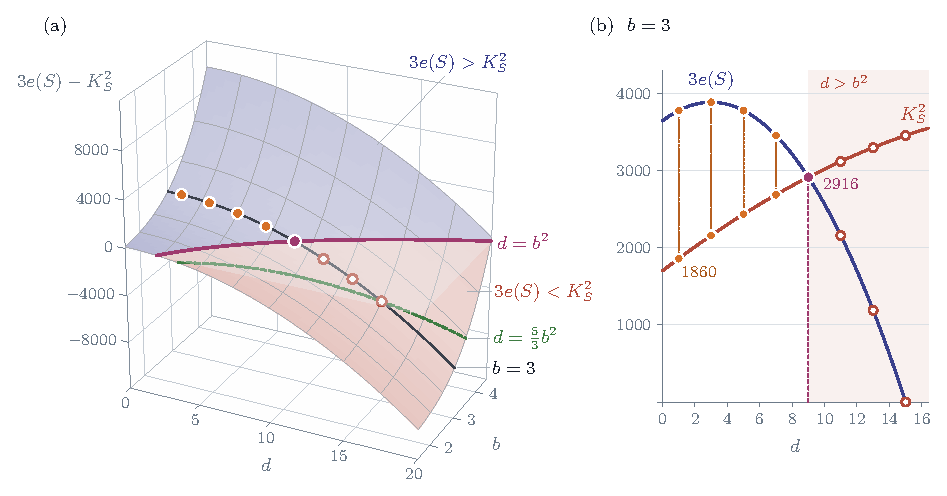
\includegraphics[width=\textwidth]{fig_bmywindow}
\caption{\Cref{thm:smoothinvariants} over the quarter plane of $(b,d)$. The
height of the surface is the defect $3e(S)-K_{S}^{2}=24(b^{4}-d^{2})$ in the
Bogomolov--Miyaoka--Yau inequality for the surface the theorem attaches to the
pair, compressed by a signed cube root so that four orders of magnitude fit
one frame; the compression is odd and monotone, so the zero locus and the sign
are the true ones. The surface is drawn indigo where the defect is positive and
clay where it is negative, and it crosses zero along $d=b^{2}$, which is
therefore the whole content of the inequality. The weaker wall $d=\tfrac53
b^{2}$, where $e(S)$ itself changes sign, is drawn dashed and lies above it.
On the line $b=3$, which is the value \Cref{prop:markman8}(iii) forces on the
fourfold, the four squarefree discriminants $d=1,3,5,7$ with $N$ an integer sit
above the wall and are marked with their drop lines; $d=9$ sits exactly on it,
the equality case, and $d=11,13,15$ sit below and are excluded.}
\label{fig:bmywindow}
\end{figure}

\begin{remark}[Status of the smooth case]\label{rem:smoothremains}
The local argument does not apply here, for a structural reason given by
\Cref{prop:smoothlocal}: the sheaf $\cE xt^{2}$ of a smooth ideal vanishes,
so both sides of \eqref{eq:heisenberg} are locally zero, and the comparison of
germs that decides \Cref{thm:candidatefails} has nothing to compare.

The surface is rigidly constrained. At $b=3$ its class, its canonical class,
its Euler characteristic, its Euler number and its two intersection numbers
with the polarisation are all determined by $d$, and they are compatible with
existence only for $d\le9$. This is the content of
\Cref{cor:fourdiscriminants}, and it restricts the construction: for all but
finitely many imaginary quadratic fields the secant construction of
\Cref{setup:markman} with smooth support is not available, whatever the
geometry of the surface.

What remains is a single existence question. For $d\in\{1,3,5,7\}$, does a
principally polarised abelian fourfold carry a smooth surface $S$ with the
invariants of \Cref{tab:smoothsupport}, and if so, does the image of
$A_{\theta}A_{\theta'}$ in $H^{1}(S,N_{S/X})$ vanish for all
$\theta,\theta'\in H^{0}(T_{X})$? The first half is a question about surfaces
in abelian fourfolds with prescribed Chern numbers, of the kind that is
answered by a construction or by a classification argument; the second is a
question about one cohomology group of one normal bundle. Neither is settled
here. The simplest surfaces of the right class are ruled out by one entry of
the table: a complete intersection of divisors in $|a\Theta|$ and
$|b'\Theta|$ has class $ab'\Theta^{2}$, so $ab'=N$, and canonical class
$(a+b')\lambda$ by adjunction, so $K_{S}\cdot\lambda=24(a+b')N$; since
$ab'=N\ge5$ forces $a+b'\ge5$, this exceeds the required $96N$. The
surface, if it exists, is not cut out by two theta divisors, nor by any two
divisors algebraically equivalent to multiples of $\Theta$; nor, by
\Cref{cor:latticeburch} below, is its ideal sheaf presented by any two bundles
whose classes lie in the subring generated by line bundles. It must also move
with $X$ to first order in every polarised direction, in the exact sense of
\Cref{prop:smoothrank}, while the injectivity that \Cref{lem:annihilation}
asks of it holds automatically when $X$ is simple (\Cref{lem:smoothinjective}).

A positive answer to both, for a surface that moves in this way, together
with an affirmative answer to \cite[Question 11.4]{Mar25b}, would produce
Weil classes on abelian
eightfolds for at most four discriminants; the other discriminants, every
$n\ge5$ and every field of degree larger than two would still have to be
reached through \Cref{prop:descent} and the propagation statement.
\end{remark}

Two of the conditions on a smooth support are decided by the table, and the
third, which \Cref{thm:factor}(iii)(a) imposes on every candidate, has an
exact form. The first is the injectivity of $H^{2}(\cO_{X})\to H^{2}(\cO_{S})$
that \Cref{lem:annihilation} below requires of every support.

\begin{lemma}[The injectivity condition for a smooth support]
\label{lem:smoothinjective}
Let $X$ be a simple complex abelian fourfold, let $V=H^{0}(T_{X})$, and let
$S\subset X$ be a smooth surface. The following are equivalent:
\begin{enumerate}[label=\textup{(\roman*)},nosep,leftmargin=2.2em]
\item the restriction $H^{2}(\cO_{X})\to H^{2}(\cO_{S})$ is injective;
\item no nonzero translation-invariant holomorphic $2$-form on $X$ restricts
  to zero on $S$;
\item $S$ is not Lagrangian for any translation-invariant holomorphic
  symplectic form on $X$;
\item the Gauss image of $S$ in $\operatorname{Gr}(2,V)\subset\PP(\bigwedge^{2}V)$
  spans $\PP(\bigwedge^{2}V)$.
\end{enumerate}
If $e(S)\ne[S]^{2}$, they hold. In particular they hold for every smooth
support of \Cref{tab:smoothsupport}, where $e(S)=12N(36-3N)$ and
$[S]^{2}=24N^{2}$ agree only for $5N=36$.
\end{lemma}

\begin{proof}
The restriction $\iota^{*}\colon H^{2}(X,\CC)\to H^{2}(S,\CC)$ is a morphism
of Hodge structures defined over $\QQ$, so it commutes with complex
conjugation, which interchanges the $(0,2)$ and $(2,0)$ parts; hence
$\iota^{*}$ is injective on $H^{0,2}(X)=H^{2}(\cO_{X})$ if and only if it is
injective on $H^{2,0}(X)=\bigwedge^{2}V^{\vee}$, the translation-invariant
$2$-forms. A holomorphic $2$-form on a compact surface is zero as a class in
$H^{2,0}(S)=H^{0}(K_{S})$ if and only if it is zero as a form; this is
(i)$\Leftrightarrow$(ii). The restriction of $p\wedge q\in\bigwedge^{2}V^{\vee}$
to $S$ is the pull-back of the Pl\"ucker coordinate $p\wedge q$ along the
Gauss map $\gamma\colon S\to\operatorname{Gr}(2,V)$, $s\mapsto T_{s}S$, as a
section of $K_{S}=\gamma^{*}\cO(1)$, so a $2$-form vanishes on $S$ if and
only if the corresponding hyperplane contains $\gamma(S)$; this is
(ii)$\Leftrightarrow$(iv).

A nonzero $2$-form on $V\cong\CC^{4}$ has rank two or four. If $\omega$ has
rank four, $\omega|_{S}=0$ says that every tangent plane of $S$ is
$\omega$-isotropic, that is, $S$ is Lagrangian for $\omega$. If
$\omega=\alpha\wedge\beta$ has rank two, with $\alpha,\beta\in V^{\vee}$
independent, then $\alpha|_{S}$ and $\beta|_{S}$ are independent
holomorphic $1$-forms on $S$, because $S$ generates the simple $X$ and a nonzero
invariant $1$-form restricts nontrivially to a generating subvariety, and
$\alpha|_{S}\wedge\beta|_{S}=0$. By the theorem of Castelnuovo and de
Franchis \cite{BHPV04} there is a fibration
$f\colon S\to C$ onto a curve of genus at least two with $\alpha|_{S}$ and
$\beta|_{S}$ pulled back from $C$. A fibre $F$ of $f$ is a curve in $X$ on
which $\alpha$ and $\beta$ vanish, so all its tangent lines lie in the fixed
plane $B=\ker\alpha\cap\ker\beta\subset V$. The abelian subvariety generated
by $F-F$ is the image of a sum map from a power of $F$, whose differential at
a general point is spanned by tangent vectors of $F$; so its tangent space
lies in $B$, its dimension is at most two, and it is nonzero because $F$ is
not a point. This contradicts the simplicity of $X$. Hence only the
rank-four case occurs, which is (ii)$\Leftrightarrow$(iii).

Finally, if $S$ is Lagrangian for a symplectic $\omega$, then $\omega$
identifies $T_{S}$ with the annihilator of $T_{S}$ in $\Omega^{1}_{X}|_{S}$,
which is the conormal bundle, so $N_{S/X}\cong\Omega^{1}_{S}$ and
$c_{2}(N_{S/X})=e(S)$; since $T_{X}$ is trivial, $c_{2}(N_{S/X})=[S]^{2}$ by
the self-intersection formula. So $e(S)\ne[S]^{2}$ excludes (iii). For the
table, \Cref{thm:smoothinvariants} gives $[S]^{2}=24N^{2}$ and
$e(S)=12N(36-3N)$ at $b=3$, and $24N^{2}=12N(36-3N)$ reads $5N=36$. For
general $b$ the two agree only when $N=\tfrac45b^{2}$, that is
$d=\tfrac35b^{2}$, whose first integral instance is $b=5$, $d=15$.
\end{proof}

\begin{remark}[The class $K_{S}-4\lambda$]\label{rem:gysinkernel}
\Cref{thm:smoothinvariants} records $K_{S}\cdot\lambda=96N$ and
$\lambda^{2}=24N$ at $b=3$, so $K_{S}\cdot\lambda=4\lambda^{2}$, and that
$K_{S}$ is never numerically proportional to $\lambda$. The sharper
statement is that
\[
  \delta=K_{S}-4\lambda\in\ker\bigl(\iota_{*}\colon H^{2}(S,\QQ)\to H^{6}(X,\QQ)\bigr),
  \qquad \delta^{2}=-12N(N-4)<0,
\]
because $\iota_{*}K_{S}=4N\Theta^{3}$ and
$\iota_{*}\lambda=\Theta\cup[S]=N\Theta^{3}$. So $\delta$ is a nonzero
algebraic class of type $(1,1)$, orthogonal by the projection formula to the
whole image of $H^{2}(X,\QQ)$ in $H^{2}(S,\QQ)$, and of negative square: the
Picard number of $S$ is at least two, and the kernel of the Gysin map on
$H^{2}(S,\QQ)$, a sub-Hodge structure, contains an algebraic class. For
general $b$ the class is $K_{S}-\tfrac{4b}{3}\lambda$, with square
$\tfrac{4N}{3}(4b^{2}-9N)$, and its vanishing is the equality case $9N=4b^{2}$
of the Hodge index bound in \Cref{thm:smoothinvariants}. This excludes none
of the four cases; it describes them.
\end{remark}

The third condition is the one that \Cref{thm:factor}(iii)(a) imposes on
every candidate and that the construction of \Cref{setup:markman} meets by
its uniformity over the moduli of principally polarised fourfolds
(\Cref{cor:markmancondition}): the object must extend to first order along
every polarised deformation of $(X,\Theta)$. For $\cF=\cI_{S}(3\Theta)$ with
$S$ smooth this is a condition on $S$. If $S$ extends along a deformation
$X_{v}$ of $X$ that keeps $\Theta$ of type $(1,1)$, then so does $\cF$.
Conversely, the obstruction $v\lrcorner\,\mathrm{At}(\cF)\in\Ext^{2}(\cF,\cF)$
has, under the edge map to $H^{1}(S,\cE xt^{1}(\cF,\cF))=H^{1}(S,N_{S/X})$ of
\Cref{rem:obstructionmoves}, the image of $v$ under
$H^{1}(T_{X})\to H^{1}(\iota^{*}T_{X})\to H^{1}(N_{S/X})$, by
\Cref{lem:edge} applied on the overlaps of a cover; and that image is the
obstruction $\operatorname{ob}_{S}(v)$ to extending the subscheme $S$ along
$X_{v}$. So condition (a) for $\cF$ is the statement that $S$ extends to
first order along every polarised deformation of $X$, and Bloch's
semiregularity map \cite{Blo72} puts it in a form that names the object it
concerns. For $S\subset X$ smooth of codimension two with normal bundle
$N=N_{S/X}$, let
\[
  \pi\colon H^{1}(S,N)\xrightarrow{\ \cong\ }H^{1}(S,N^{\vee}\otimes K_{S})
  \xrightarrow{\ j\ }H^{1}(S,\iota^{*}\Omega^{1}_{X}\otimes K_{S})
  \xrightarrow{\ \iota_{*}\ }H^{3}(X,\Omega^{1}_{X})
\]
be the composite of $N\cong N^{\vee}\otimes\bigwedge^{2}N$, of the conormal
inclusion $N^{\vee}\to\iota^{*}\Omega^{1}_{X}$ tensored with $K_{S}$, and of
the Gysin map, with $K_{X}\cong\cO_{X}$. This is the semiregularity map of
Bloch for codimension two, and it satisfies
$\pi(\operatorname{ob}_{S}(v))=v\lrcorner[S]$ for every $v\in H^{1}(X,T_{X})$.

\begin{lemma}[Duality]\label{lem:blochduality}
Under Serre duality $H^{1}(X,T_{X})\times H^{3}(X,\Omega^{1}_{X})\to H^{4}(\cO_{X})=\CC$,
\[
  \{v\in H^{1}(X,T_{X}):S\ \text{extends to first order along }v\}
  =\pi\bigl(H^{1}(S,N)\bigr)^{\perp}.
\]
\end{lemma}

\begin{proof}
$S$ extends along $v$ if and only if $\operatorname{ob}_{S}(v)=0$, and
$\operatorname{ob}_{S}$ is the composite of the restriction
$r\colon H^{1}(X,T_{X})\to H^{1}(S,\iota^{*}T_{X})$ with the map induced by
$\iota^{*}T_{X}\to N$. The Serre dual of $r$ is the Gysin map
$\iota_{*}\colon H^{1}(S,\iota^{*}\Omega^{1}_{X}\otimes K_{S})\to H^{3}(X,\Omega^{1}_{X}\otimes K_{X})$,
and the Serre dual of $H^{1}(\iota^{*}T_{X})\to H^{1}(N)$ is the map
$H^{1}(N^{\vee}\otimes K_{S})\to H^{1}(\iota^{*}\Omega^{1}_{X}\otimes K_{S})$
induced by the conormal inclusion. So the dual of $\operatorname{ob}_{S}$ is
$\iota_{*}\circ j$, which is $\pi$ after the identification
$N\cong N^{\vee}\otimes K_{S}$, and the kernel of a linear map is the
annihilator of the image of its dual.
\end{proof}

\begin{proposition}[The first-order condition is a rank condition]
\label{prop:smoothrank}
Let $S\subset X$ be a smooth surface with $[S]=N\Theta^{2}$, $N\ne0$. Then
$\pi(H^{1}(S,N))\supseteq\Theta\cup H^{0,2}(X)$, a subspace of dimension six,
and the following are equivalent:
\begin{enumerate}[label=\textup{(\roman*)},nosep,leftmargin=2.2em]
\item $S$ extends to first order along every polarised deformation of
  $(X,\Theta)$, that is, $\cI_{S}(3\Theta)$ satisfies condition (a) of
  \Cref{thm:factor}(iii);
\item $\pi(H^{1}(S,N))=\Theta\cup H^{0,2}(X)$;
\item $\operatorname{rank}\pi=6$, the least value possible.
\end{enumerate}
In particular a smooth secant support is as far from semiregular in Bloch's
sense as a surface with this class can be: $\dim\ker\pi=h^{1}(N)-6$, with
$h^{1}(N)=2h^{0}(N)-2\chi(\cO_{S})+24N^{2}\ge8-2\chi(\cO_{S})+24N^{2}$, which
is at least $88$, $296$, $568$ and $904$ for $N=5,6,7,8$.
\end{proposition}

\begin{proof}
The polarised deformations form $P=\{v:v\lrcorner\Theta=0\}$, of dimension
ten in $H^{1}(T_{X})=V\otimes H^{0,1}(X)$. For $z\in H^{0,2}(X)$ the pairing
is $\langle v,\Theta\cup z\rangle=(v\lrcorner\Theta)\cup z$, so
$\Theta\cup H^{0,2}(X)\subseteq P^{\perp}$; the map $z\mapsto\Theta\cup z$ is
injective by hard Lefschetz, so this subspace has dimension six, and
$\dim P^{\perp}=16-10=6$, so $P^{\perp}=\Theta\cup H^{0,2}(X)$. By
\Cref{lem:blochduality}, (i) says $P\subseteq\pi(H^{1}(N))^{\perp}$, that is
$\pi(H^{1}(N))\subseteq P^{\perp}$. On the other hand
$\pi(\operatorname{ob}_{S}(v))=v\lrcorner[S]=2N\,\Theta\cup(v\lrcorner\Theta)$,
and $v\mapsto v\lrcorner\Theta$ is surjective onto $H^{0,2}(X)$, because
$\Theta$ identifies $V$ with $\overline{V}^{\vee}$ and the contraction becomes
the exterior product $V\otimes\overline{V}^{\vee}\to\bigwedge^{2}\overline{V}^{\vee}$.
So $\pi(H^{1}(N))\supseteq\Theta\cup H^{0,2}(X)$ always, and (i), (ii), (iii)
are equivalent. For $h^{1}(N)$, Riemann--Roch with $c_{1}(N)=K_{S}$ and
$c_{2}(N)=[S]^{2}=24N^{2}$ gives $\chi(N)=2\chi(\cO_{S})-24N^{2}$, Serre
duality with $N^{\vee}\otimes K_{S}\cong N$ gives $h^{2}(N)=h^{0}(N)$, and
$h^{0}(N)\ge4$ because the four translation vector fields map injectively to
$H^{0}(N)$: a translation vector field tangent to $S$ everywhere would restrict
to a nowhere vanishing vector field on $S$, so that $e(S)=c_{2}(T_{S})=0$,
while a secant support has $e(S)=12N(36-3N)\ne0$ for $N=5,6,7,8$ by
\Cref{thm:smoothinvariants}.
\end{proof}

\begin{remark}[What the rank condition asks]\label{rem:smoothrank}
\Cref{prop:smoothrank} does not decide the condition; it converts it into the
statement that the kernel of Bloch's map has codimension exactly six, as it
has for the complete intersections $\Theta\cap\Theta_{x}$, which do move with
$X$. The kernel of $\pi$ is
$j^{-1}\bigl(V^{\vee}\otimes\ker(H^{1}(K_{S})\to H^{3}(\cO_{X}))\bigr)$, and
for $q(S)=4$ it is the image in $H^{1}(N^{\vee}\otimes K_{S})$ of
$H^{0}(\Omega^{1}_{S}\otimes K_{S})$ modulo $V^{\vee}\otimes H^{0}(K_{S})$. A
count with $\chi(\Omega^{1}_{S}\otimes K_{S})=2\chi(\cO_{S})+24N^{2}$ and
$h^{1}(T_{S})\le h^{0}(N)+12$ shows the rank condition to be consistent with
every inequality available, so no exclusion follows at this level; what
would decide it is $\ker\pi$ for an actual surface, and no candidate surface
is known.
\end{remark}

\subsection{Depth and the local obstruction}
\label{ssec:depth}

By \Cref{prop:smoothlocal}, at a smooth point of the support there is
nothing local to compare. This is a special case of a much more general
statement, and the general statement shows exactly which supports
\Cref{thm:candidatefails} and \Cref{cor:localobstruction} exclude and which
lie beyond their reach. The dividing line is neither smoothness nor the local
complete intersection property, but depth.

\begin{theorem}[Cohen--Macaulay supports carry no local obstruction]%
\label{thm:cmvanishing}
Let $Y$ be a smooth variety with $\omega_{Y}\cong\cO_{Y}$, let $Z\subset Y$ be
a closed subscheme of codimension two, and let $p\in Z$. If the local ring
$\cO_{Z,p}$ is Cohen--Macaulay, then
\[
  \cE xt^{q}(\cI_{Z},\cI_{Z})_{p}=0\qquad\text{for every }q\ge2 ,
\]
and the same holds for $\cI_{Z}\otimes L$ for every line bundle $L$.
Consequently both sides of \eqref{eq:heisenberg} have vanishing germ at $p$,
and \Cref{lem:edge} decides nothing there.
\end{theorem}

\begin{proof}
Twisting by $L$ changes no $\cE xt$ sheaf, so take $F=\cI_{Z}$. Write
$A=\cO_{Y,p}$, a regular local ring of dimension $m$, and $I=\cI_{Z,p}$. By
hypothesis $A/I$ is Cohen--Macaulay of dimension $m-2$, so
$\operatorname{depth}A/I=m-2$, and the Auslander--Buchsbaum formula gives
\[
  \operatorname{pd}_{A}(A/I)=m-\operatorname{depth}_{A}(A/I)=2 .
\]
From the exact sequence $0\to I\to A\to A/I\to0$ with $A$ free it follows that
$\operatorname{pd}_{A}I=1$. A module of projective dimension one has a free
resolution of length one, so $\Ext^{q}_{A}(I,M)=0$ for every $A$-module $M$
and every $q\ge2$; taking $M=I$ gives the vanishing, since
$\cE xt^{q}(\cI_{Z},\cI_{Z})_{p}=\Ext^{q}_{A}(I,I)$. The last assertion
follows from \Cref{lem:edge}: the right side of \eqref{eq:heisenberg} is
$z\cdot\id_{F}$ with $z\in H^{2}(\cO_{Y})$ and has vanishing germs, and the
left side lies in a sheaf whose $\cE xt^{2}$ factor is zero.
\end{proof}

\begin{remark}[Sharpness of the hypothesis]%
\label{rem:cmsharp}
Two observations show that \Cref{thm:cmvanishing} is the right statement.

First, Cohen--Macaulayness is strictly weaker than the more familiar
conditions that could be imposed instead. Among codimension two germs in
$\CC^{4}$, the smooth germ $(x_{1},x_{2})$, two planes meeting along a line,
$(x_{1},x_{2}x_{3})$, three planes meeting along a line,
$(x_{1},x_{2}x_{3}x_{4})$, the double plane $(x_{1}^{2},x_{2})$ and the
quadric cone $(x_{1},x_{2}^{2}-x_{3}x_{4})$ are complete intersections. The
fat plane $(x_{1},x_{2})^{2}$ and the cone over the twisted cubic are the
ideals of $2\times2$ minors of
$\left(\begin{smallmatrix}x_{1}&x_{2}&0\\
0&x_{1}&x_{2}\end{smallmatrix}\right)$ and of
$\left(\begin{smallmatrix}x_{1}&x_{2}&x_{3}\\
x_{2}&x_{3}&x_{4}\end{smallmatrix}\right)$, of the expected codimension two,
so they are Cohen--Macaulay by the Hilbert--Burch theorem, although neither
is a local complete intersection, both needing three generators. By
\Cref{thm:cmvanishing}, $\cE xt^{2}(\cI_{Z},\cI_{Z})$ vanishes at all seven.
Reducedness, irreducibility and the complete intersection property are
therefore all irrelevant; what matters is the projective dimension, which by
Auslander--Buchsbaum is a matter of depth.

Second, the vanishing fails at the germs that the construction of
\Cref{setup:markman} produces. Two planes meeting at a point and three planes
meeting pairwise at a point are reduced surface germs that become
disconnected when the point is removed, so they have depth $1$: at least $1$
because they are reduced, and at most $1$ by the connectedness theorem
recalled below. A plane with an embedded point has depth $0$. By Auslander--Buchsbaum the projective
dimensions of $\cO_{Z,p}$ are $3$, $3$ and $4$, and the proof of
\Cref{cor:cmdichotomy}(i) below gives $\cE xt^{q}(\cI_{Z},\cI_{Z})_{p}\ne0$
for $q=2$, $2$ and $3$. By Hartshorne's connectedness theorem, a scheme whose local ring at $p$
is Cohen--Macaulay is connected in codimension one at $p$, so a support with
two components through $p$ meeting only at $p$ is never Cohen--Macaulay
there. This is precisely the configuration analysed in
\Cref{lem:localproducts}.
\end{remark}

\begin{corollary}[The local dichotomy]%
\label{cor:cmdichotomy}
Let $(X,t)$ be a polarised abelian variety of dimension $n\ge4$ and $F$ a
perfect complex with $\ch(F)=au_{t}+bv_{t}$, $(a,b)\ne(0,0)$, whose germ at
each point is the germ of $\cI_{Z}\otimes L$ for a subscheme $Z$ of
codimension two, and let $p\in Z$.
\begin{enumerate}[label=\textup{(\roman*)},leftmargin=2.6em]
\item If $Z$ is not Cohen--Macaulay at $p$, then
  $\cE xt^{q}(\cI_{Z},\cI_{Z})_{p}\ne0$ for $q=\operatorname{pd}\cI_{Z,p}\ge2$,
  so the comparison of germs of \Cref{lem:edge} has room at $p$. If moreover
  $Z$ has at $p$ two smooth branches of codimension two meeting
  transversally, as in \Cref{lem:localproducts} and
  \Cref{cor:localobstruction}, then $F$ does not satisfy the weakened
  criterion, nor does $\Phi(F\boxtimes F_{2})$ for any secant $F_{2}$.
\item If $Z$ is Cohen--Macaulay, then there is no local obstruction at any
  point. Condition (b) of \Cref{thm:factor}(iii) is then a single global
  condition: it holds if and only if the image of $A_{\theta}A_{\theta'}$ in
  $H^{1}\bigl(Z,\cE xt^{1}(\cI_{Z},\cI_{Z})\bigr)$ vanishes for all
  $\theta,\theta'\in H^{0}(T_{X})$, the scalar on the right of
  \eqref{eq:heisenberg} being forced by the trace. Condition (a), the
  extension of $F$ to first order along the polarised deformations, is
  not affected by the depth and remains to be checked.
\end{enumerate}
In case (ii), $\cI_{Z}$ has projective dimension one at every point, so it is
locally the ideal of maximal minors of a Hilbert--Burch matrix; if $Z$ is
moreover smooth, then $\cE xt^{1}(\cI_{Z},\cI_{Z})=N_{Z/X}$ and the invariants
of $Z$ are those of \Cref{thm:smoothinvariants}.
\end{corollary}

\begin{proof}
(i) Put $A=\cO_{X,p}$, of dimension $n$, and $I=\cI_{Z,p}$. Since $A/I$ is not
Cohen--Macaulay, $\operatorname{depth}A/I<\dim A/I\le n-2$, so
$\operatorname{pd}_{A}(A/I)\ge3$ by the Auslander--Buchsbaum formula and
$q=\operatorname{pd}_{A}I\ge2$. In a minimal free resolution
$F_{\bullet}\to I$ the entries of the differentials lie in the maximal ideal
$\mathfrak m$, so $\Ext^{q}_{A}(I,I)$, the cokernel of
$\Hom(F_{q-1},I)\to\Hom(F_{q},I)$, surjects onto
$\Hom(F_{q},I)\otimes A/\mathfrak m\ne0$ by Nakayama's lemma. At two
transversal branches the conclusion is \Cref{thm:candidatefails} and
\Cref{cor:localobstruction}. (ii) \Cref{thm:cmvanishing} gives
$\cE xt^{q}=0$ for $q\ge2$ at every point, so the local-to-global spectral
sequence for $\Ext^{2}(\cI_{Z},\cI_{Z})$ has only the two rows
$H^{1}(\cE xt^{1})$ and $H^{2}(\cO_{X})$, and these lie in different steps of
the filtration, the second being the subgroup of scalars. The right side of
\eqref{eq:heisenberg} lies in that subgroup, so its image in the quotient
$H^{1}(\cE xt^{1})$ is zero, and (b) forces the image of the left side there
to vanish. Conversely, if that image vanishes, then
$\mathrm{At}(F)^{2}=z\cdot\id_{F}$ for some
$z\in H^{2}(\cO_{X})\otimes\bigwedge^{2}H^{1,0}$, the map
$z\mapsto z\cdot\id_{F}$ being injective because its composite with the
trace is multiplication by $\rk F=1$; taking traces,
$z=\operatorname{tr}\mathrm{At}(F)^{2}=-d\,t^{2}$ by the last assertion of
\Cref{thm:factor}(iii), which is (b). The statement on projective dimension
was established in the proof of \Cref{thm:cmvanishing}, and the Hilbert--Burch theorem is the
structure theorem for ideals of projective dimension one over a regular local
ring; the last clause is \Cref{prop:smoothlocal} together with
\Cref{thm:smoothinvariants}.
\end{proof}

\begin{remark}[Normalisation and depth]%
\label{rem:normalisationcm}
\Cref{cor:cmdichotomy} explains the tension recorded in
\Cref{rem:normalisedpoints}. The partial normalisation performed in
\Cref{setup:markman} separates the two branches at an isolated double point,
and separating them is exactly what would make the local ring
Cohen--Macaulay there; the normalisation is thus an attempt to reach case
(ii). \Cref{rem:normalisedpoints} shows that the attempt cannot succeed:
normalising every isolated point moves $\chi(\cO_{\widetilde Z})$ to $50N$,
while the secant plane demands $(d+9)(27-d)=72N-4N^{2}$, and the two agree
only at $N=11/2$. Repairing the depth destroys the Chern character, and
keeping the Chern character keeps a point where the depth fails. This is the
precise form of the obstruction, and it explains why a construction
assembled from intersections of translates of a polarisation cannot be made
to work: by \Cref{cor:localobstruction} such a chain always has a point of
the bad type, and by \Cref{rem:normalisedpoints} it cannot be separated
without leaving the plane.
\end{remark}

\subsection{Hilbert--Burch resolutions}
\label{ssec:hilbertburch}

\Cref{cor:cmdichotomy} leaves one class of supports and, beside the
extension along the polarised deformations, one condition on them.
The class consists of the Cohen--Macaulay subschemes of codimension two, and
for these the proof of \Cref{thm:cmvanishing} gives more than the vanishing
it was used for: the ideal sheaf has projective dimension one at every point.
This is the Hilbert--Burch shape, whose invariants are polynomials in the twists.

\begin{setupenv}[A resolution of the support]\label{setup:burch}
Let $(X,\Theta)$ be a principally polarised abelian fourfold with
$\NS(X)_{\QQ}=\QQ\Theta$, let $Z\subset X$ be Cohen--Macaulay of codimension
two, and suppose $\cI_{Z}$ admits a global resolution
\begin{equation}\label{eq:burchres}
  0\longrightarrow E_{1}\stackrel{\varphi}{\longrightarrow}E_{0}
  \longrightarrow\cI_{Z}\longrightarrow0,
  \qquad \rk E_{0}=r+1,\quad\rk E_{1}=r,
\end{equation}
with $E_{0}=\bigoplus_{i=1}^{r+1}\cO(e_{i}\Theta)$ and
$E_{1}=\bigoplus_{j=1}^{r}\cO(f_{j}\Theta)$ sums of line bundles. Put
$p_{i}=e_{i}+b$ and $q_{j}=f_{j}+b$.
\end{setupenv}

\begin{lemma}[The resolution in moments]\label{lem:burchmoments}
In \Cref{setup:burch}, $\ch(\cI_{Z}(b\Theta))=u_{\Theta}+b\,v_{\Theta}$ holds
if and only if
\begin{equation}\label{eq:burchsystem}
  \sum_{i=1}^{r+1}p_{i}^{\,k}-\sum_{j=1}^{r}q_{j}^{\,k}=c_{k},
  \qquad k=0,1,2,3,4,
  \qquad (c_{k})=(1,\;b,\;-d,\;-db,\;d^{2}).
\end{equation}
The equation at $k=0$ is the rank count and is automatic. In addition,
$\varphi$ can be injective only if $\max_{i}e_{i}\ge\max_{j}f_{j}$, and
$\cO_{X}$ embeds in $E_{0}^{\vee}$ only if $\min_{i}e_{i}\le0$.
\end{lemma}

\begin{proof}
From \eqref{eq:burchres}, $\ch(\cI_{Z})=\ch(E_{0})-\ch(E_{1})$, so
$\ch(\cI_{Z}(b\Theta))=\sum_{i}e^{p_{i}\Theta}-\sum_{j}e^{q_{j}\Theta}$.
Comparing coefficients of $\Theta^{k}/k!$ with those of
$u_{\Theta}+bv_{\Theta}$, which are the $c_{k}$ displayed, gives
\eqref{eq:burchsystem}. For the last two statements, recall that on an
abelian variety $\Hom(\cO(f\Theta),\cO(e\Theta))=H^{0}(\cO((e-f)\Theta))$
vanishes unless $e\ge f$. If $\varphi$ is injective, each summand of $E_{1}$
must map nonzero to $E_{0}$, which requires $\max_{i}e_{i}\ge f_{j}$ for
every $j$. Dualising \eqref{eq:burchres} and using $\cI_{Z}^{\vee}=\cO_{X}$
gives an injection $\cO_{X}\hookrightarrow E_{0}^{\vee}$, which requires
$-e_{i}\ge0$ for some $i$.
\end{proof}

The case $r=1$ consists of the complete intersections, and it is settled for
every $b$ and every $d$ by an argument that needs no search.

\begin{theorem}[No complete intersection supports a secant object]%
\label{thm:noci}
Let $(X,\Theta)$ be a principally polarised abelian fourfold with
$\NS(X)_{\QQ}=\QQ\Theta$, let $d>0$ and $b\ge1$. No complete intersection
$Z=D_{1}\cap D_{2}$ of two divisors satisfies
$\ch(\cI_{Z}(b\Theta))=u_{\Theta}+b\,v_{\Theta}$.
\end{theorem}

\begin{proof}
Such a $Z$ is \Cref{setup:burch} with $r=1$, the resolution being the Koszul
complex of the two equations. Put $w(x)=x^{2}+d$, which is strictly positive
on $\RR$ because $d>0$, and read \eqref{eq:burchsystem} in the combinations
$c_{k+2}+d\,c_{k}$ for $k=0,1,2$. Those three numbers are
\[
  c_{2}+dc_{0}=-d+d=0,\qquad
  c_{3}+dc_{1}=-db+db=0,\qquad
  c_{4}+dc_{2}=d^{2}-d^{2}=0,
\]
so that
\[
  \sum_{i}w(p_{i})\,p_{i}^{\,k}=\sum_{j}w(q_{j})\,q_{j}^{\,k},
  \qquad k=0,1,2 .
\]
The two sides are the moments of order $0$, $1$ and $2$ of the positive
measures $\nu_{P}=\sum_{i}w(p_{i})\delta_{p_{i}}$ and
$\nu_{Q}=\sum_{j}w(q_{j})\delta_{q_{j}}$, so those measures have the same
mass, the same mean and the same variance. At $r=1$ the measure $\nu_{Q}$ has
one atom, hence variance zero, so $\nu_{P}$ has variance zero as well, and a
positive measure with two atoms has variance zero only if the atoms coincide.
Hence $p_{1}=p_{2}$, and equality of the means forces $q_{1}=p_{1}$. The
resolution \eqref{eq:burchres} then cancels, and $\cI_{Z}\cong\cO(e_{1}\Theta)$
would be a line bundle, which the ideal sheaf of a subscheme of codimension
two is not.

In terms of the divisors, the same computation shows that their degrees
$a_{1}$ and $a_{2}$ would have to satisfy $a_{1}+a_{2}=\tfrac43b$ and
$(b-a_{1})(b-a_{2})=\tfrac12\bigl(\tfrac13b^{2}+d\bigr)$; the quadratic with
roots $b-a_{1}$ and $b-a_{2}$ then has discriminant $-\tfrac29b^{2}-2d<0$, so
the degrees are not even real.
\end{proof}

For $r\ge2$ the moment conditions alone no longer decide the question. The
Chern characters of the bundles of \Cref{setup:burch}, and of every bundle
built from line bundles, lie in one lattice, and the secant plane meets that
lattice only along a congruence. Write a class $\xi\in\QQ[\Theta]/(\Theta^{5})$
as $\xi=\sum_{k=0}^{4}c_{k}(\xi)\,\Theta^{k}/k!$, as in
\Cref{lem:burchmoments}, so that $c_{k}(e^{j\Theta})=j^{k}$, and let
$\cL_{\Theta}$ be the subgroup generated by the classes
$e^{j\Theta}=\ch\cO_{X}(j\Theta)$, $j\in\ZZ$. It is a subring, since
$e^{a\Theta}e^{b\Theta}=e^{(a+b)\Theta}$, and it contains $\ch$ of every
bundle obtained from line bundles algebraically equivalent to multiples of
$\Theta$ by direct sums, tensor products, duals, exterior and symmetric
powers, kernels of surjections and cokernels of injections between such
bundles, and extensions;
in particular the kernel bundles
$M_{m\Theta}=\ker\bigl(H^{0}(\cO(m\Theta))\otimes\cO_{X}\to\cO_{X}(m\Theta)\bigr)$,
of class $m^{4}-e^{m\Theta}$, and their duals and twists.

\begin{lemma}[Binomial moments]\label{lem:binomialmoments}
Define $m_{k}(\xi)\in\QQ$, $0\le k\le4$, by
\begin{equation}\label{eq:stirling}
  c_{i}(\xi)=\sum_{k=0}^{i}S(i,k)\,k!\,m_{k}(\xi),
\end{equation}
where $S(i,k)$ are the Stirling numbers of the second kind; explicitly
\begin{gather*}
  m_{0}=c_{0},\qquad m_{1}=c_{1},\qquad m_{2}=\tfrac12(c_{2}-c_{1}),\\
  m_{3}=\tfrac16(c_{3}-3c_{2}+2c_{1}),\qquad
  m_{4}=\tfrac1{24}(c_{4}-6c_{3}+11c_{2}-6c_{1}).
\end{gather*}
Then $\xi\in\cL_{\Theta}$ if and only if $m_{k}(\xi)\in\ZZ$ for $k=0,\dots,4$.
\end{lemma}

\begin{proof}
For $\xi=\sum_{j}a_{j}e^{j\Theta}$ one has $c_{i}(\xi)=\sum_{j}a_{j}j^{i}$,
and $j^{i}=\sum_{k}S(i,k)\,k!\binom{j}{k}$, so \eqref{eq:stirling} holds
with $m_{k}(\xi)=\sum_{j}a_{j}\binom{j}{k}\in\ZZ$. Conversely, the five
vectors $\bigl(\binom{j}{0},\dots,\binom{j}{4}\bigr)$ for $j=0,\dots,4$
form a unitriangular matrix, so every integer vector $(m_{0},\dots,m_{4})$
is an integer combination of them, and the corresponding
$\sum_{j=0}^{4}a_{j}e^{j\Theta}$ lies in $\cL_{\Theta}$ with the prescribed
moments. Since \eqref{eq:stirling} is invertible over $\QQ$, the moments
determine $\xi$.
\end{proof}

Equivalently, sending $e^{j\Theta}$ to $x^{j}$ identifies
$\QQ[\Theta]/(\Theta^{5})$ with $\QQ[y]/(y^{5})$, $y=x-1$, the class
$e^{j\Theta}$ going to $(1+y)^{j}$; then $m_{k}(\xi)$ is the coefficient of
$y^{k}$ and $\cL_{\Theta}$ is $\ZZ[y]/(y^{5})$.

\begin{theorem}[The secant plane and the lattice of line bundles]
\label{thm:lattice}
For $(a,b)\in\ZZ^{2}$ and $d\ge1$,
\[
  m\bigl(a\,u_{\Theta}+b\,v_{\Theta}\bigr)
  =\Bigl(a,\ b,\ -\frac{ad+b}{2},\ \frac{3ad+2b-bd}{6},\
  \frac{ad^{2}-11ad+6bd-6b}{24}\Bigr).
\]
Consequently $a\,u_{\Theta}+b\,v_{\Theta}\in\cL_{\Theta}$ if and only if
\begin{gather*}
  ad\equiv b\pmod 2,\qquad 3ad+2b-bd\equiv0\pmod 6,\\
  ad^{2}-11ad+6bd-6b\equiv0\pmod{24}.
\end{gather*}
For $a=1$ and $b=3$ the moments are
$\bigl(1,3,-\tfrac{d+3}{2},1,\tfrac{(d+9)(d-2)}{24}\bigr)$, and
$u_{\Theta}+3v_{\Theta}\in\cL_{\Theta}$ if and only if $d$ is odd and
$24\mid(d+9)(d-2)$, that is, if and only if
\[
  d\equiv15\ \text{or}\ 23\pmod{24}.
\]
\end{theorem}

\begin{proof}
In the variable $y=x-1$ put
$L=\log(1+y)=y-\tfrac12y^{2}+\tfrac13y^{3}-\tfrac14y^{4}$ modulo $y^{5}$.
Under $e^{j\Theta}\mapsto x^{j}$ the class $\Theta$ goes to $L$, hence
$u_{\Theta}\mapsto1-\tfrac d2L^{2}+\tfrac{d^{2}}{24}L^{4}$ and
$v_{\Theta}\mapsto L-\tfrac d6L^{3}$. With
$L^{2}=y^{2}-y^{3}+\tfrac{11}{12}y^{4}$, $L^{3}=y^{3}-\tfrac32y^{4}$ and
$L^{4}=y^{4}$ modulo $y^{5}$, the coefficients of $1,y,\dots,y^{4}$ in
$a\,u_{\Theta}+b\,v_{\Theta}$ are the five displayed expressions, and the
congruences are the integrality of the last three. For $b=3$ the second
reads $3d+6-3d=6$, so $m_{3}=1$, and the third reads
$d^{2}+7d-18=(d+9)(d-2)$. Modulo $8$ the condition is $8\mid(d+1)(d-2)$
with $d$ odd, hence $d\equiv7\pmod8$; modulo $3$ it is $3\mid d(d-2)$, hence
$d\equiv0,2\pmod3$; together $d\equiv15,23\pmod{24}$.
\end{proof}

\begin{corollary}[Split resolutions, for every rank and every twist]
\label{cor:latticeburch}
Let $Z\subset X$ be Cohen--Macaulay of codimension two with a resolution
$0\to E_{1}\to E_{0}\to\cI_{Z}\to0$ in which $\ch E_{0}$ and $\ch E_{1}$ both
lie in $\cL_{\Theta}$: for instance \Cref{setup:burch} with any rank and any
twists, or $E_{0}$ and $E_{1}$ built from such line bundles and from the
bundles $M_{m\Theta}$ by the operations listed above. If
$\ch(\cI_{Z}(3\Theta))=u_{\Theta}+3v_{\Theta}$, then $d\equiv15$ or
$23\pmod{24}$. In particular this never happens for the four discriminants
of \Cref{cor:fourdiscriminants}.
\end{corollary}

\begin{proof}
$\ch(\cI_{Z}(3\Theta))=e^{3\Theta}(\ch E_{0}-\ch E_{1})\in\cL_{\Theta}$, and
\Cref{thm:lattice} applies.
\end{proof}

\begin{remark}[What the congruence measures]\label{rem:latticedefect}
The fractional part of $m_{4}$ is the invariant that separates the secant
plane from the line bundles. For $d\in\{1,3,5,7\}$ it is
$-\tfrac{5}{12},\tfrac12,\tfrac34,\tfrac13$ modulo $\ZZ$, and any object with
Chern character $u_{\Theta}+3v_{\Theta}$ must carry a class outside
$\cL_{\Theta}$ with exactly that defect. Two checks. A point has
$m=(0,0,0,0,1/24)$, and the partial normalisation of \Cref{setup:markman} at
$(d+9)(2d-1)$ isolated points shifts $m_{4}$ by $(d+9)(2d-1)/24$; since
$(d+9)(d-2)+(d+9)(2d-1)=3(d+9)(d-1)\equiv0\pmod{24}$ for odd $d$, the
unnormalised chain, which lies in $\cL_{\Theta}$, is moved onto the plane by
exactly the right defect, as it must be. For a smooth support the class of
the structure sheaf has $m(\cO_{S})=\bigl(0,0,N,-3N,N(83-2N)/12\bigr)$, and
$N(83-2N)/12$ is not an integer for $N\in\{5,6,7,8\}$; so a smooth secant
support is a surface whose structure sheaf is not in the line-bundle
subring, unlike every complete intersection of translates of $\Theta$ and
every degeneracy locus of a map between bundles in $\cL_{\Theta}$. The
Fourier--Mukai transforms of line bundles and the push-forwards of line
bundles along isogenies do have classes outside $\cL_{\Theta}$, which is why
the semi-homogeneous bundles need the separate argument of
\Cref{thm:noblocks}.
\end{remark}

The lattice constrains the classes of the two terms of a resolution; their
ranks constrain the Chern classes, because a vector bundle of rank $s$ has
$c_{k}=0$ for $k>s$, and on a fourfold this bites for $s\le3$.

\begin{proposition}[Resolutions of rank one and two]\label{prop:lowrankburch}
Let $(X,\Theta)$ be a principally polarised abelian fourfold, let $b\ge1$
and $d>0$, and let $Z\subset X$ be of codimension two with a resolution
\[
  0\longrightarrow E_{1}\longrightarrow E_{0}\longrightarrow\cI_{Z}
  \longrightarrow0
\]
by vector bundles of ranks $r$ and $r+1$, and with
$\ch(\cI_{Z}(b\Theta))=u_{\Theta}+b\,v_{\Theta}$.
\begin{enumerate}[label=\textup{(\roman*)},nosep,leftmargin=2.2em]
\item $r\ge2$, whatever the bundles. Equivalently, $Z$ is not the zero locus
  of a section of a vector bundle of rank two.
\item If $r=2$ and the Chern classes of $E_{1}$ are polynomials in $\Theta$,
  as they are when $\Hdg^{2}(X)=\QQ\Theta$ and $\Hdg^{4}(X)=\QQ\Theta^{2}$,
  then, writing $c_{1}(E_{1}(b\Theta))=a\Theta$ with $a\in\ZZ$,
  \[
    3d-b^{2}-4ab\equiv0\pmod{12}.
  \]
  At $b=3$ this says $d\equiv3\pmod4$.
\end{enumerate}
In particular, at the discriminants $d=1$ and $d=5$ of
\Cref{cor:fourdiscriminants}, a resolution whose Chern classes are
polynomials in $\Theta$ has $r\ge3$.
\end{proposition}

\begin{proof}
Put $E=E_{1}(b\Theta)$, $G=E_{0}(b\Theta)$ and $F=\cI_{Z}(b\Theta)$, so that
$0\to E\to G\to F\to0$ is exact and $c(G)=c(E)\,c(F)$. Newton's identities
applied to $\ch(F)=1+b\Theta-\frac d2\Theta^{2}-\frac{db}{6}\Theta^{3}
+\frac{d^{2}}{24}\Theta^{4}$ give, with $N=\frac12(b^{2}+d)$,
\[
  c(F)=1+b\Theta+N\Theta^{2}+\tfrac{bN}{3}\Theta^{3}
  +\tfrac{N(b^{2}-3d)}{12}\Theta^{4}.
\]
Since $E$ and $G$ are vector bundles, $c_{k}(E)=0$ for $k>r$ and
$c_{k}(G)=0$ for $k>r+1$.

(i) Let $r=1$ and $\ell=c_{1}(E)$, so that $c(G)=(1+\ell)\,c(F)$. The rank
two bundle $G$ has $c_{3}(G)=\frac{bN}{3}\Theta^{3}+N\ell\,\Theta^{2}=0$, and
cup product with $\Theta^{2}$ is an isomorphism $H^{2}(X,\QQ)\to H^{6}(X,\QQ)$
by hard Lefschetz, so $\ell=-\frac b3\Theta$. Then
\[
  c_{4}(G)=c_{4}(F)+\ell\,c_{3}(F)
  =N\Bigl(\frac{b^{2}-3d}{12}-\frac{b^{2}}{9}\Bigr)\Theta^{4}
  =-\frac{N(b^{2}+9d)}{36}\,\Theta^{4},
\]
which is not zero, since $N>0$ and $d>0$. A section of a rank two bundle $V$
vanishing in codimension two exactly on $Z$ gives the Koszul resolution
$0\to\det V^{\vee}\to V^{\vee}\to\cI_{Z}\to0$, which has $r=1$; conversely,
at $r=1$ the map $E_{1}\to E_{0}$ is a section of $E_{0}\otimes E_{1}^{\vee}$
with zero locus $Z$.

(ii) Let $r=2$, and write $c_{1}(E)=a\Theta$ and $c_{2}(E)=\frac m2\Theta^{2}$
with $a,m\in\ZZ$, since $\Theta$ and $\frac12\Theta^{2}$ are primitive
integral classes. Now $c_{3}(E)=c_{4}(E)=0$, and the rank three bundle $G$
has
\[
  c_{4}(G)=c_{4}(F)+c_{1}(E)\,c_{3}(F)+c_{2}(E)\,c_{2}(F)=0 .
\]
Integrating, with $\int_{X}\Theta^{4}=24$, and dividing by $2N$ gives
$6m=3d-b^{2}-4ab$. By Riemann--Roch with trivial Todd class,
$\chi(E)=\int_{X}\ch_{4}(E)=a^{4}-2a^{2}m+\frac12m^{2}$ is an integer, so $m$
is even, which is the congruence. At $b=3$ it reads $3(d-3)\equiv12a\equiv0$
modulo $12$, that is, $d\equiv3\pmod4$.
\end{proof}

\begin{remark}[What the ranks exclude]\label{rem:lowrankburch}
Part (i) extends \Cref{thm:noci} from two divisors to the zero locus of a
section of any rank two bundle, stable or not, so the construction of Serre
produces no secant support; it holds for every $X$, with no condition on
$\NS(X)$. Part (ii) holds for arbitrary bundles whose Chern classes are
polynomials in $\Theta$, not only for sums of line bundles, and at $b=3$ it
excludes $r=2$ whenever $d\not\equiv3\pmod4$. The integrality of
the Chern classes of $E_{0}$ is automatic, since
$c(E_{0}(b\Theta))=c(E_{1}(b\Theta))\,c(F)$ and $c(F)$ is integral, so it is
the vanishing above the rank, and not integrality, that constrains. Neither
condition restricts $r\ge3$: a bundle of rank four has no vanishing Chern
class on a fourfold, and at $r=3$ the only condition, $c_{4}(E)=0$, involves
$E$ alone.
\end{remark}

\Cref{cor:latticeburch} says where a split resolution can have the right
Chern character. A stronger statement holds: no object with a split
resolution satisfies the criterion, at any rank and for any discriminant
(\Cref{thm:nosplit}). It
rests on a necessary condition that we isolate, because it applies to
every object and can be tested on any candidate before any global
computation is attempted.

\begin{lemma}[Morphisms to a line bundle are killed by $H^{2}(\cO)$]
\label{lem:annihilation}
Let $(X,t)$ be a polarised abelian variety of dimension $n\ge3$, let $F$ be
a perfect complex with $\ch(F)=au_{t}+bv_{t}$, $(a,b)\ne(0,0)$, which
satisfies the weakened criterion of \Cref{setup:criterion}, and let $L$ be a
line bundle with $c_{1}(L)\in\QQ\,t$. Then for every $m\in\ZZ$, every
morphism $p\colon F\to L[m]$, every morphism $q\colon L[m]\to F$, and every
$z\in H^{2}(\cO_{X})$,
\[
  z\cdot p=0\ \ \text{in }\Hom(F,L[m+2]),\qquad
  z\cdot q=0\ \ \text{in }\Hom(L[m],F[2]),
\]
where $z\cdot(\,\cdot\,)$ is the $H^{*}(\cO_{X})$-module structure on
morphisms in $D^{b}(X)$. In particular, if $F=\cI_{Z}\otimes L'$ for a closed
subscheme $Z$ and a line bundle $L'$ with $c_{1}(L')\in\QQ t$, then the
restriction $H^{n-2}(\cO_{X})\to H^{n-2}(\cO_{Z})$ is injective.
\end{lemma}

\begin{proof}
For a constant bivector $\pi$ the class
$x_{\pi}=(\tfrac d2\,\pi\lrcorner\,t^{2},0,\pi)$ preserves $\ch(F)$ by
\Cref{thm:factor}(ii), so $\operatorname{ev}_{F}(x_{\pi})=0$ by hypothesis.
The Hochschild action is by natural transformations $\id\to\id[2]$ of
$D^{b}(X)$, so for $p\colon F\to L[m]$ we have
$\operatorname{ev}_{L[m]}(x_{\pi})\circ p=p\circ\operatorname{ev}_{F}(x_{\pi})=0$,
where $\operatorname{ev}_{L[m]}=\operatorname{ev}_{L}[m]$. By
\eqref{eq:evsplit}, $\operatorname{ev}_{L}(x_{\pi})=c_{\pi}\cdot\id_{L}$ with
$c_{\pi}=\tfrac12\,\pi\lrcorner\,(\lambda^{2}+d\,t^{2})\in H^{0,2}(X)$ and
$\lambda=c_{1}(L)=e\,t$, that is,
$c_{\pi}=\tfrac{e^{2}+d}{2}\,\pi\lrcorner\,t^{2}$. Since $e^{2}+d>0$ and
$\pi\mapsto\pi\lrcorner\,t^{2}$ is an isomorphism from
$H^{0}(\bigwedge^{2}T_{X})$ onto $H^{0,2}(X)$, as in the proof of
\Cref{thm:factor}(iii), $c_{\pi}$ runs over all of $H^{2}(\cO_{X})$ as $\pi$
varies; as $(c_{\pi}\cdot\id_{L})\circ p=c_{\pi}\cdot p$, this proves the
assertion for $p$. The assertion for $q$ follows in the same way from the
square
$\operatorname{ev}_{F}(x_{\pi})\circ q=q\circ\operatorname{ev}_{L[m]}(x_{\pi})$.
For the last assertion, apply the first to the inclusion
$p\colon\cI_{Z}\otimes L'\to L'$. After twisting by $L'^{-1}$, the sequence
$0\to\cI_{Z}\to\cO_{X}\to\cO_{Z}\to0$ gives an exact sequence
\[
  \Ext^{2}(\cO_{Z},\cO_{X})\longrightarrow H^{2}(\cO_{X})
  \longrightarrow\Ext^{2}(\cI_{Z},\cO_{X}),
\]
in which the second map is $z\mapsto z\cdot p$. So $z\cdot p=0$ for all $z$
means that the first map is surjective, and by Serre duality, $\omega_{X}$
being trivial, the first map is dual to the restriction
$H^{n-2}(\cO_{X})\to H^{n-2}(\cO_{Z})$.
\end{proof}

\begin{theorem}[No two-term complex of powers of the polarisation satisfies
the criterion]\label{thm:nosplit}
Let $(X,t)$ be a polarised abelian variety of dimension $n\ge3$ and $M$ an
ample line bundle with $c_{1}(M)\in\QQ t$. Let $A$ and $B$ be direct sums of
tensor powers $M^{\otimes e}$, $e\in\ZZ$, let $\varphi\colon A\to B$ be any
morphism, and let $F$ be the cone of $\varphi$, or any shift of it. If $F\ne0$
and $\ch(F)=au_{t}+bv_{t}$ with $(a,b)\ne(0,0)$, then $F$ does not satisfy
the weakened criterion. In particular, no object with a resolution
$0\to E_{1}\to E_{0}\to F\to0$ by sums of powers of $M$ satisfies it,
whatever the rank.
\end{theorem}

\begin{proof}
A pair of summands $M^{\otimes e}$ of $A$ and $M^{\otimes e}$ of $B$ joined
by a nonzero entry of $\varphi$, which is then a nonzero scalar, can be
cancelled without changing the cone up to isomorphism; do this until no such
pair remains. If $A=0$ or $B=0$ after cancelling, $F$ is a shifted sum of
line bundles, $\operatorname{ev}_{F}(x_{\pi})$ is diagonal with the nonzero
entries $c_{\pi}\cdot\id$ of the proof of \Cref{lem:annihilation}, and the
criterion fails as in \Cref{cor:noline}; so suppose both are nonzero and
consider the triangle $A\xrightarrow{\varphi}B\xrightarrow{\;q\;}F\to A[1]$.
Let $M^{\otimes b_{j}}$ be a summand of $B$, $\iota_{j}$ its inclusion into
$B$, and $q_{j}=q\circ\iota_{j}\colon M^{\otimes b_{j}}\to F$. Applying
$\Hom(M^{\otimes b_{j}},-)$ to the triangle gives the exact sequence
\[
  \Hom(M^{\otimes b_{j}},A[2])\xrightarrow{\;\varphi_{*}\;}
  \Hom(M^{\otimes b_{j}},B[2])\xrightarrow{\;q_{*}\;}
  \Hom(M^{\otimes b_{j}},F[2]),
\]
and $z\cdot q_{j}=q_{*}(z\cdot\iota_{j})$ for $z\in H^{2}(\cO_{X})$. Now
$\Hom(M^{\otimes b_{j}},B[2])=\bigoplus_{k}H^{2}(M^{\otimes(b_{k}-b_{j})})$,
and $H^{2}(M^{\otimes m})=0$ for $m\ne0$: for $m>0$ by Kodaira vanishing,
$\omega_{X}$ being trivial, and for $m<0$ because a negative line bundle on
an abelian variety has cohomology only in degree $n\ge3$. So $z\cdot\iota_{j}$
is the element with component $z$ in the summand $k=j$ and zero elsewhere. It
lies in the image of $\varphi_{*}$ only if there is
$\psi\in\Hom(M^{\otimes b_{j}},A[2])=\bigoplus_{i}H^{2}(M^{\otimes(a_{i}-b_{j})})$
with $(\varphi\circ\psi)_{j}=\sum_{i}\varphi_{ji}\psi_{i}=z$; but $\psi_{i}\ne0$
forces $a_{i}=b_{j}$, and for such $i$ the entry $\varphi_{ji}$ is a scalar,
zero after the cancellation. So $z\cdot q_{j}\ne0$ for every $z\ne0$, which
contradicts \Cref{lem:annihilation}. The last assertion is the case of a
resolution, where $F\cong\coker\varphi$ is the cone of $\varphi\colon E_{1}\to E_{0}$.
\end{proof}

The powers of the polarisation are not the only bundles on which the
compensated Poisson classes act by scalars. The same holds for every bundle
whose Atiyah class is a multiple of the identity, and on an abelian variety
these are the semi-homogeneous bundles of Mukai \cite{Muk78}. The argument of
\Cref{thm:nosplit} goes through for them, with the cohomology of the fibre
product of two isogenies in place of the cohomology of a power of $\Theta$.
We state the result in a self-contained form.

\begin{definition}[Isogeny blocks]\label{def:block}
Let $(X,\Theta)$ be a polarised abelian variety. An \emph{isogeny block} is a
vector bundle $E=\pi_{*}L$, where $\pi\colon Y\to X$ is an isogeny and $L$ is
a line bundle on $Y$ with $c_{1}(L)=\nu\,\pi^{*}\Theta$ in $H^{2}(Y,\QQ)$,
$\nu\in\QQ$; its \emph{slope} is $\nu$, so that $c_{1}(E)=\nu\deg(\pi)\,\Theta$.
The block is \emph{simple} if $\tau_{g}^{*}L\not\cong L$ for every nonzero
$g\in\ker\pi$. The powers $\cO(e\Theta)$ are the blocks with $\pi=\id$.
\end{definition}

\begin{lemma}[Three properties of a block]\label{lem:blocks}
Let $E=\pi_{*}L$ be an isogeny block of slope $\nu$ on an abelian $n$-fold.
\begin{enumerate}[label=\textup{(\roman*)},nosep]
\item $\mathrm{At}(E)=\nu\Theta\cdot\id_{E}$; hence for a constant bivector
  $\pi$ the compensated class $x_{\pi}$ of \Cref{thm:factor}(ii) acts by
  $\operatorname{ev}_{E}(x_{\pi})=\tfrac{\nu^{2}+d}{2}\,(\pi\lrcorner\,\Theta^{2})\cdot\id_{E}$,
  and \Cref{lem:annihilation} holds with $E$ in place of the line bundle $L$.
\item For a second block $E'=\pi'_{*}L'$ of slope $\nu'$,
  $\Ext^{q}(E',E)=H^{q}(Z,M)$ with $Z=Y'\times_{X}Y$, a disjoint union of
  abelian varieties isogenous to $X$, and $M$ a line bundle whose class on
  each component is $(\nu-\nu')$ times the pullback of $\Theta$. If
  $\nu\ne\nu'$ and $n\ge3$ then $\Ext^{2}(E',E)=0$. If $E$ is simple then
  $\Ext^{2}(E,E)=H^{2}(\cO_{X})\cdot\id_{E}$.
\item A simple block is $\mu$-stable with respect to $\Theta$; hence a
  nonzero morphism between simple blocks of the same slope is an
  isomorphism.
\end{enumerate}
\end{lemma}

\begin{proof}
(i) Since $\pi$ is \'etale, $\pi^{*}\Omega^{1}_{X}=\Omega^{1}_{Y}$ and $\pi_{*}$
is exact, so the first jet sequence of $\pi_{*}L$ is the direct image of
that of $L$, and $\mathrm{At}(\pi_{*}L)$ is the image of $\mathrm{At}(L)$
under $\pi_{*}\colon\Ext^{1}_{Y}(L,L\otimes\pi^{*}\Omega^{1}_{X})\to
\Ext^{1}_{X}(\pi_{*}L,\pi_{*}L\otimes\Omega^{1}_{X})$. As $\mathrm{At}(L)=c_{1}(L)\cdot\id_{L}
=\nu\,\pi^{*}\Theta\cdot\id_{L}$, the projection formula gives
$\nu\Theta\cdot\id_{\pi_{*}L}$. Then \eqref{eq:evgeneral} with a scalar Atiyah
class gives the value of $\operatorname{ev}_{E}(x_{\pi})$, and the proof of
\Cref{lem:annihilation} used nothing else about $L$.

(ii) Adjunction for the finite \'etale $\pi'$, flat base change along the
cartesian square with vertices $Z$, $Y'$, $Y$, $X$, and the projection formula
give $\Ext^{q}_{X}(\pi'_{*}L',\pi_{*}L)=H^{q}(Y',L'^{-1}\otimes\pi'^{*}\pi_{*}L)
=H^{q}(Z,p'^{*}L'^{-1}\otimes p^{*}L)$, with $p,p'$ the two projections; the
class of $M=p'^{*}L'^{-1}\otimes p^{*}L$ is $(\nu-\nu')$ times the pullback of
$\Theta$ on every component, which is an abelian variety finite \'etale over
$Y'$. A line bundle on an abelian $n$-fold whose class is a positive
multiple of an ample class has cohomology only in degree $0$, and one whose
class is a negative multiple only in degree $n$, by Kodaira vanishing and
Serre duality with trivial canonical bundle; so $H^{2}(Z,M)=0$ when
$\nu\ne\nu'$ and $n\ge3$. When $E'=E$, the components of $Y\times_{X}Y$ are
the graphs of the translations by $g\in\ker\pi$, on which $M$ restricts to
$L^{-1}\otimes\tau_{g}^{*}L\in\Pic^{0}(Y)$; a nontrivial element of $\Pic^{0}$
has no cohomology, so $\Ext^{q}(E,E)=\bigoplus_{g}H^{q}(\cO_{Y})$ over the
$g$ with $\tau_{g}^{*}L\cong L$, which for a simple block is $g=0$ alone, and
$H^{q}(\cO_{Y})=H^{q}(\cO_{X})$ through $\pi$.

(iii) The pullback $\pi^{*}E=\bigoplus_{g\in\ker\pi}\tau_{g}^{*}L$ is a direct
sum of line bundles of one slope, hence $\mu$-semistable, and semistability
descends along the finite \'etale $\pi$; so $E$ is semistable. If $F\subset E$
is a saturated subsheaf of the same slope, then $\pi^{*}F\subset\pi^{*}E$ is
a saturated subsheaf of the same slope of a direct sum of pairwise
non-isomorphic line bundles, the $\tau_{g}^{*}L$ being distinct because the
block is simple, hence a partial sum $\bigoplus_{g\in S}\tau_{g}^{*}L$; it is
invariant under the translations by $\ker\pi$, which permute the summands
transitively, so $S$ is empty or everything and $F=0$ or $F=E$. Finally, a
nonzero morphism $f$ between $\mu$-stable bundles of the same slope is
injective and generically surjective, so the two bundles have the same rank;
for blocks of the same slope $\nu$ they then have the same $c_{1}$, since
$c_{1}(E)=\nu\,\rk(E)\,\Theta$, and $\det f$ is a nonzero section of a
numerically trivial line bundle, hence nowhere zero. So $f$ is an
isomorphism.
\end{proof}

\begin{theorem}[No two-term complex of simple blocks satisfies the criterion]
\label{thm:noblocks}
Let $(X,\Theta)$ be a polarised abelian variety of dimension $n\ge3$, let $A$
and $B$ be direct sums of simple isogeny blocks, let $\varphi\colon A\to B$
be any morphism and let $F$ be the cone of $\varphi$ or a shift of it. If
$F\ne0$ and $\ch(F)=au_{\Theta}+bv_{\Theta}$ with $(a,b)\ne(0,0)$, then $F$
does not satisfy the weakened criterion. In particular, no object with a
resolution $0\to E_{1}\to E_{0}\to F\to0$ by sums of simple isogeny blocks
satisfies it, whatever the rank.
\end{theorem}

\begin{proof}
Cancel, by Gaussian elimination in the two-term complex, every pair of
isomorphic blocks of $A$ and $B$ joined by an entry of $\varphi$ that is an
isomorphism; this changes neither the cone nor the block structure of the
remaining terms. By \Cref{lem:blocks}(iii), every remaining entry between
blocks of the same slope is zero. If $A$ or $B$ is empty after cancelling,
$F$ is a shifted sum of blocks, on each of which $\operatorname{ev}(x_{\pi})$
is a nonzero scalar by (i). Otherwise the rest is the proof of
\Cref{thm:nosplit} with \Cref{lem:blocks} in place of the vanishing of
$H^{2}(M^{\otimes m})$. For a block $E'$ of $B$ with inclusion $\iota$ and
$q'=q\circ\iota\colon E'\to F$, the class $z\cdot\iota\in\Hom(E',B[2])$ has
component $z\cdot\id_{E'}\ne0$ in $\Ext^{2}(E',E')=H^{2}(\cO_{X})\cdot\id_{E'}$
by (ii). It lies in the image of $\varphi_{*}$ only if
$\sum_{i}\varphi_{ji}\psi_{i}=z\cdot\id_{E'}$ for some
$\psi_{i}\in\Ext^{2}(E',A_{i})$, and $\psi_{i}\ne0$ forces $A_{i}$ to have
the slope of $E'$ by (ii), for which $\varphi_{ji}=0$. So $z\cdot q'\ne0$,
contradicting \Cref{lem:annihilation} in the form given by (i).
\end{proof}

\begin{remark}[Semi-homogeneous bundles]\label{rem:blocks}
By Mukai \cite{Muk78}, the simple isogeny blocks are exactly the simple
semi-homogeneous bundles, a bundle $E$ being semi-homogeneous if for every
$x$ there is $P\in\Pic^{0}(X)$ with $\tau_{x}^{*}E\cong E\otimes P$; and
every semi-homogeneous bundle on a variety with $\NS(X)_{\QQ}=\QQ\Theta$ is
an iterated extension of such blocks and their twists by $\Pic^{0}$. We do
not use this. In these terms, \Cref{thm:noblocks} says that the bundles in a
Hilbert--Burch resolution of a candidate cannot all have scalar Atiyah
class. The obstruction is always the same: the compensated Poisson classes
act on a block by the scalar $\tfrac{\nu^{2}+d}{2}\,\pi\lrcorner\,\Theta^{2}$,
which would vanish only for $\nu^{2}=-d$, and cones of maps between blocks
inherit the scalar through the summand inclusions, because $\Ext^{2}$
between blocks of different slopes vanishes. A candidate must therefore be
built from a bundle whose Atiyah class is not a scalar, that is, one which
is not projectively flat.
\end{remark}

\begin{corollary}[Split resolutions and the remaining shapes]
\label{cor:disjointroutes}
Let $(X,\Theta)$ be a principally polarised abelian fourfold.
\begin{enumerate}[label=\textup{(\roman*)},nosep]
\item No secant object of rank one whose support has a resolution
  \eqref{eq:burchres} by sums of powers of $\Theta$ satisfies the weakened
  criterion, for any $r$, any twists and any $d$, whether or not its matrix
  degenerates in codimension two.
\item If a secant object $\cI_{Z}(b\Theta)$ satisfies the criterion, then
  $Z$ has no point at which two smooth branches of codimension two meet
  transversally, no two-term resolution of $\cI_{Z}$ splits into powers of
  $\Theta$ or into simple semi-homogeneous bundles, and the restriction
  $H^{2}(\cO_{X})\to H^{2}(\cO_{Z})$ is injective. If $Z$ is
  Cohen--Macaulay, $\cI_{Z}$ has projective dimension one. If $b=3$ and $Z$
  is smooth, then $d\le9$, so $d\in\{1,3,5,7\}$ when $N=(9+d)/2$ is an
  integer as in \Cref{setup:markman}, the two terms of a resolution do not
  both have classes in $\cL_{\Theta}$, and when $X$ is simple the
  injectivity is automatic.
\item At $b=3$, smooth supports and split resolutions are disjoint, for
  every rank and every twist of the resolution: a smooth support forces
  $d\le9$, and a resolution by bundles with classes in $\cL_{\Theta}$ forces
  $d\equiv15,23\pmod{24}$, hence $d\ge15$, so that, even without (i), no
  support could have both properties.
\end{enumerate}
\end{corollary}

\begin{proof}
Part (i) is \Cref{thm:nosplit} with $M=\cO_{X}(\Theta)$, the resolution
\eqref{eq:burchres} presenting $\cI_{Z}(b\Theta)$ as the cone of
$\varphi\otimes\cO(b\Theta)$. In (ii), the branches are excluded by
\Cref{cor:cmdichotomy}(i), projective dimension one comes from
\Cref{cor:cmdichotomy}(ii), the non-splitting from \Cref{thm:nosplit} and
\Cref{thm:noblocks}, the injectivity from the last assertion of
\Cref{lem:annihilation}, the bound on $d$ from
\Cref{cor:fourdiscriminants}, the statement on the two terms from
\Cref{cor:latticeburch}, and the automatic injectivity from
\Cref{lem:smoothinjective}. Part (iii) compares
\Cref{cor:fourdiscriminants} with \Cref{cor:latticeburch}: no $d\le9$ is
congruent to $15$ or $23$ modulo $24$.
\end{proof}


\part{Weil classes of CM fields}\label{part:cmfields}
\section{Weil classes of every CM field}\label{sec:cmfields}

The Weil classes of an imaginary quadratic field are the case $m=1$ of a
construction that makes sense for every CM field $F$ of degree $2m$, and the
methods of this paper apply to the question whether those classes are
algebraic. Every theorem of \Cref{sec:construction} that turns the conjecture
for a Weil family into a propagation statement is a theorem about a connected
period domain, a flat class on it, a group whose rational points act with
dense orbits, and a base point where the class is a polynomial in divisor
classes, and none of these four ingredients depends on the field being
quadratic. This section carries the four over to every CM field; the only
one that needs a new argument is the base point, which
\Cref{thm:cmbasepoint} supplies. Nothing here is conditional on a question
about semiregularity, because the base point is a CM point: the Weil classes
there are written out as polynomials with rational coefficients in divisor
classes, each divisor class is algebraic by the Lefschetz theorem on $(1,1)$
classes, and products of algebraic classes are algebraic. Nothing is claimed
about the
whole Hodge ring at a CM point, which can contain classes that are not
polynomials in divisor classes.

\subsection{The families}

\begin{setupenv}[Weil type for a CM field]\label{setup:cmfield}
Let $F$ be a CM field of degree $2m$ with maximal totally real subfield
$F_{0}$, and write $\alpha\mapsto\bbar\alpha$ for the nontrivial automorphism
of $F/F_{0}$, which is complex conjugation under every embedding. The real
places of $F_{0}$ are $\tau_{1},\dots,\tau_{m}$, and each extends to a
conjugate pair $\sigma_{\tau},\bbar\sigma_{\tau}$ of embeddings of $F$ into
$\CC$. Let $V$ be an $F$-vector space of dimension $2n$, let
$H\colon V\times V\to F$ be a nondegenerate hermitian form, $F$-linear in the
first variable, and fix a totally imaginary $\xi\in F^{\times}$, that is
$\bbar\xi=-\xi$. Put
\[
  E(x,y)=\Tr_{F/\QQ}\bigl(\xi\,H(x,y)\bigr),
\]
a nondegenerate alternating $\QQ$-bilinear form with
$E(\alpha x,y)=E(x,\bbar\alpha y)$. For each $\tau$ let
$V_{\tau}=V\otimes_{F_{0},\tau}\RR$, a vector space of dimension $2n$ over
$F\otimes_{F_{0},\tau}\RR\cong\CC$, and let $(p_{\tau},q_{\tau})$ be the
signature of the hermitian form $H_{\tau}$ induced by $H$ on it. We say that
$(V,H)$ is of \emph{$(F,n)$-Weil type} if $p_{\tau}=q_{\tau}=n$ for every
$\tau$, and we call the class of $(-1)^{n}\det H$ in
$F_{0}^{\times}/\Nm_{F/F_{0}}(F^{\times})$ its discriminant $\delta$; it is
totally positive, and for $F=K$ it is the discriminant of \Cref{def:disc}. A
polarised abelian variety $(A,\iota,E)$ of dimension $2mn$ with
$\iota\colon F\to\End^{0}(A)$ and $H^{1}(A,\QQ)\cong V$ as $F$-modules with
polarisation $E$ is of $(F,n,\delta)$-Weil type when $(V,H)$ is. As in
\Cref{lem:Kspace}, we work throughout with $V=H^{1}$; a complex structure on
$V_{\RR}$ is the same datum as one on the tangent space. The Weil
classes of $A$ are
\[
  W_{F}(A)=\textstyle\bigwedge^{2n}_{F}V\;\subseteq\;\bigwedge^{2n}_{\QQ}V
  =H^{2n}(A,\QQ),
\]
the $\QQ$-subspace whose complexification is
$\bigoplus_{\sigma}\bigwedge^{2n}V_{\sigma}$, where $V_{\sigma}=V\otimes_{F,\sigma}\CC$
runs over the $2m$ eigenspaces of $F$ on $V_{\CC}$; it is a one-dimensional
$F$-vector space, of dimension $2m$ over $\QQ$. Write
\begin{quote}
$\mathbf{W}(F,n,\delta)$: every abelian variety of $(F,n,\delta)$-Weil type
has algebraic Weil classes.
\end{quote}
The period domain $\cD_{F}$ is the set of complex structures $J$ on
$V_{\RR}$ commuting with $F$ and polarised by $E$, and the group
$G_{F}=\Res_{F_{0}/\QQ}\SU(V,H)$ acts on it. We fix an arithmetic subgroup
$\Gamma\subset G_{F}(\QQ)$ and write $\cS_{F}=\Gamma\backslash\cD_{F}$ for the
quotient, $p\colon\cD_{F}\to\cS_{F}$ for the projection,
$\pi\colon\cA\to\cS_{F}$ for the universal family and
$\Sigma_{F}\subseteq\cD_{F}$ for the set of $s$ at which $W_{F}(A_{s})$ is
algebraic. For $m=1$ this is \Cref{setup:family} and \Cref{setup:shimura},
with $\omega_{s}$ a generator of the line.
\end{setupenv}

\begin{remark}[Every such abelian variety is a member]\label{rem:cmmember}
If $A$ is any abelian variety with a CM field $F\subseteq\End^{0}(A)$ such
that $\dim_{F}H^{1}(A,\QQ)=2n$ and $\dim V_{\sigma}^{1,0}=n$ for every
embedding $\sigma$, then $A$ is of $(F,n,\delta)$-Weil type for some
$\delta$: the Rosati involution of any polarisation restricts to a positive
involution of $F$, hence to conjugation, and the argument of
\Cref{lem:hermform} writes the polarisation as $\Tr_{F/\QQ}(\xi H)$ for a
unique hermitian $H$, whose signatures are then forced by the Hodge numbers
as in \Cref{prop:cmweil}(i). These are exactly the abelian varieties whose
Weil classes for $F$ are Hodge classes, in the sense of \cite{MZ99}, so
$\mathbf{W}(F,n,\delta)$ over all $(F,n,\delta)$ is the statement that all
Weil classes of all CM fields are algebraic.
\end{remark}

\begin{proposition}[The Weil classes of a CM field]\label{prop:cmweil}
Keep \Cref{setup:cmfield}, with $(V,H)$ of $(F,n)$-Weil type.
\begin{enumerate}[label=\textup{(\roman*)},leftmargin=2.6em,itemsep=2pt]
\item A polarised complex structure $J$ is the same as an $H_{\tau}$-orthogonal
  decomposition $V_{\tau}=V_{\tau}^{+}\oplus V_{\tau}^{-}$ for every $\tau$,
  with $H_{\tau}$ definite of the sign of $\mathrm{Im}\,\sigma_{\tau}(\xi)$ on
  $V_{\tau}^{+}$ and of the opposite sign on $V_{\tau}^{-}$; then
  $\dim V^{1,0}_{\sigma_{\tau}}=\dim V_{\tau}^{+}=n$ and
  $\dim V^{1,0}_{\bbar\sigma_{\tau}}=\dim V_{\tau}^{-}=n$, so every class in
  $W_{F}(A_{J})$ is of type $(n,n)$. The spaces $W_{F}(A_{J})$ form a flat
  subsystem $W_{F}$ of $R^{2n}\pi_{*}\QQ$ of rank $2m$ on which $G_{F}$ acts
  trivially, and $\cD_{F}\cong\prod_{\tau}\cD_{n,n}$ is connected of
  dimension $mn^{2}$.
\item If one nonzero element of $W_{F}(A)$ is algebraic, every element is.
\item If $\Hg(A_{s})=G_{F}$, the Hodge ring of $A_{s}$ is generated by
  $\NS(A_{s})_{\QQ}$ and by $W_{F}$, so the Hodge conjecture for $A_{s}$ in
  every degree is equivalent to the algebraicity of $W_{F}$. For $n\ge2$ the
  space $\NS(A_{s})_{\QQ}$ is the $m$-dimensional space of classes
  $\eta_{t}=[E(t\,\cdot,\cdot)]$, $t\in F_{0}$.
\item Two members of $(F,n,\delta)$-Weil type have isomorphic $(V,H)$, so
  every one of them is a fibre of $\pi$.
\end{enumerate}
\end{proposition}

\begin{proof}
(i) A complex structure commuting with $F$ preserves each $V_{\tau}$, since
$F_{0}\otimes\RR$ acts diagonally, and is $\CC$-linear on it for the
structure $F\otimes_{F_{0},\tau}\RR\cong\CC$, so it is $\pm\sqrt{-1}$ on two
complementary $\CC$-subspaces $V_{\tau}^{\pm}$. Write
$\sigma_{\tau}(\xi)=\sqrt{-1}\,r_{\tau}$ with $r_{\tau}\in\RR^{\times}$. For
$x\in V^{\epsilon}_{\tau}$ and $y\in V^{\epsilon'}_{\tau}$ one has
$H_{\tau}(Jx,Jy)=\epsilon\epsilon'H_{\tau}(x,y)$, so
$E(Jx,Jy)=E(x,y)$ forces $E(x,y)=0$ for $\epsilon\ne\epsilon'$, and replacing
$x$ by $\sqrt{-1}\,x$ then forces $H_{\tau}(x,y)=0$: the decomposition is
orthogonal. For $x\in V^{\epsilon}_{\tau}$,
$E(x,Jx)=2\,\mathrm{Re}\bigl(\sqrt{-1}\,r_{\tau}\,
\overline{\epsilon\sqrt{-1}}\,H_{\tau}(x,x)\bigr)=2\epsilon r_{\tau}H_{\tau}(x,x)$,
so positivity is the sign condition stated. Conversely such a decomposition
defines a polarised $J$. Under $V_{\tau}\otimes_{\RR}\CC=V_{\sigma_{\tau}}
\oplus V_{\bbar\sigma_{\tau}}$ the space $V^{1,0}$, the $\sqrt{-1}$-eigenspace
of $J$ on $V_{\CC}$, meets $V_{\sigma_{\tau}}$ in the image of $V_{\tau}^{+}$
and $V_{\bbar\sigma_{\tau}}$ in the conjugate of the image of $V_{\tau}^{-}$,
which gives the two equalities of dimensions. Since $H_{\tau}$ has signature
$(n,n)$ and is definite, of opposite signs, on the complementary orthogonal
subspaces $V_{\tau}^{\pm}$, both have dimension $n$. So each $V_{\sigma}$ is
the sum of its intersections with $V^{1,0}$ and $V^{0,1}$, both of dimension
$n$, and a generator $\alpha_{\sigma}$ of $\bigwedge^{2n}V_{\sigma}$ is of
type $(n,n)$. The subspace $\bigwedge^{2n}_{F}V$ of $H^{2n}(A_{s},\QQ)$ is
defined by the action of $F$ on $V$ alone and does not depend on $s$, so it
is flat; $\SU(V,H)$ acts on $\bigwedge^{2n}_{F}V$ by the $F$-determinant,
which is $1$. Finally, the choice of $V_{\tau}^{+}$ is a point of the bounded
symmetric domain of $\SU(V_{\tau},H_{\tau})\cong\SU(n,n)$, of dimension
$n^{2}$, and $\cD_{F}$ is the product over $\tau$.

(ii) For $\alpha\in\cO_{F}$ the endomorphism $\iota(\alpha)$ acts on
$\bigwedge^{2n}_{F}V$ by $\alpha^{2n}$, through an algebraic correspondence,
so the algebraic classes in $W_{F}$ form a $\QQ$-subspace stable under
multiplication by every $\alpha^{2n}$. By the polarisation identity, in
characteristic zero every product $x_{1}\cdots x_{2n}$ of elements of a field
is a rational combination of $2n$-th powers of sums of the $x_{i}$; taking
$x_{2}=\dots=x_{2n}=1$ shows that the $2n$-th powers span $F$ over $\QQ$, and
since every element of $F$ is a rational multiple of an element of $\cO_{F}$,
so do the $\alpha^{2n}$ with $\alpha\in\cO_{F}$. Hence the $\QQ$-span of
$\{\alpha^{2n}w\}$ is $Fw=W_{F}$ for every $w\ne0$.

(iii) Hodge classes are the invariants of the Hodge group, which here is
$G_{F}$. Over $\CC$ it is $\prod_{\tau}\SL(U_{\tau})$ with
$U_{\tau}=V_{\sigma_{\tau}}$, and
$H$ identifies $V_{\bbar\sigma_{\tau}}$ with $U_{\tau}^{\vee}$, so
$\bigwedge^{*}V_{\CC}=\bigotimes_{\tau}\bigwedge^{*}(U_{\tau}\oplus U_{\tau}^{\vee})$
with the $\tau$-th factor of the group acting on the $\tau$-th tensor factor
alone. The invariants of a product group in a tensor product of
representations are the tensor product of the invariants, and the invariants
of $\SL(U)$ in $\bigwedge^{*}(U\oplus U^{\vee})$ are generated by the pairing
$\psi\in U\otimes U^{\vee}$ and the two determinants, by the computation of
\Cref{thm:hdgcount}. The classes $\eta_{t}$ are Hodge classes: $J$ commutes
with $t$ and preserves $E$, hence preserves the $F_{0}$-twisted form
$E_{t}=E(t\,\cdot,\cdot)=\Tr(\xi tH)$, which for totally positive $t$ is again
a polarisation of $A_{s}$. The complexified span of the $\eta_{t}$ is
$\bigoplus_{\tau}\CC\psi_{\tau}$, and the complexification of $W_{F}$
contains all the determinants. So the $\QQ$-algebra generated by $\NS_{\QQ}$
and $W_{F}$ has complexification equal to the ring of invariants, hence
equals $\Hdg^{*}(A_{s})$. Since divisor classes are algebraic, the conjecture
reduces to $W_{F}$, and by (ii) to one class. For the last sentence, the
invariants in $\bigwedge^{2}V_{\CC}$ are $\bigoplus_{\tau}\CC\psi_{\tau}$ when
$n\ge2$: a summand $\bigwedge^{2}U_{\tau}$ or $\bigwedge^{2}U_{\tau}^{\vee}$
has an $\SL(U_{\tau})$-invariant only if $\dim U_{\tau}=2n$ equals $2$, and a
summand mixing two different $\tau$ has none. So $\NS(A_{s})_{\QQ}$ has
dimension $m$, and it contains the classes $\eta_{t}$, which form an
$m$-dimensional space because $t\mapsto\eta_{t}$ is injective on $F_{0}$, $E$
being nondegenerate.

(iv) Two hermitian forms over $F/F_{0}$ of the same rank, the same
discriminant and the same signature at every real place of $F_{0}$ are
isomorphic \cite[Ch.~10, \S6]{Sch85}. So the datum $(F,n,\delta)$ determines
$(V,H)$ up to isomorphism, and the Hodge structure of any member is, by (i), a
polarised complex structure on that $V_{\RR}$, that is a point of $\cD_{F}$.
\end{proof}

\begin{lemma}[The Hodge group of a very general member]\label{lem:cmgeneric}
Keep \Cref{setup:cmfield}. For every $s\in\cD_{F}$ one has
$\Hg(A_{s})\subseteq G_{F}$, and there is a countable union $Z$ of proper
closed analytic subsets of $\cD_{F}$ such that $\Hg(A_{s})=G_{F}$ for every
$s\notin Z$.
\end{lemma}

\begin{proof}
The Hodge group of $A_{s}$ commutes with $\End^{0}(A_{s})\supseteq F$ and
preserves $E$, so it lies in $\Res_{F_{0}/\QQ}\mathrm{U}(V,H)$: an $F$-linear
map preserving $E=\Tr_{F/\QQ}(\xi H)$ preserves $H$, because $H$ is recovered
from $E$ and the action of $F$ as in \Cref{lem:hermform}. It fixes every Hodge
class, in particular the Weil classes, which are Hodge classes by
\Cref{prop:cmweil}(i); an element $g$ of $\Res_{F_{0}/\QQ}\mathrm{U}(V,H)$ acts
on $\bigwedge^{2n}_{F}V$ by $\det_{F}(g)$, so $\det_{F}(g)=1$ and
$g\in G_{F}$.

For the second statement let $T$ be the set of rational tensors
$t\in\bigoplus_{a,b}V^{\otimes a}\otimes(V^{\vee})^{\otimes b}$ that are not
fixed by $G_{F}$, a countable set, and for $t\in T$ let $Z_{t}$ be the set of
$s$ at which $t$ is a Hodge class, of type $(p,p)$ with $2p=a-b$, for the
Hodge structure induced by $A_{s}$. The condition is that $t$ lies in the
$p$-th step of the Hodge filtration, which varies holomorphically with $s$, so
$Z_{t}$ is a closed analytic subset of $\cD_{F}$. It is proper. Otherwise $t$
is fixed by $h_{s}(\mathrm{U}(1))$ for every $s\in\cD_{F}$, where $h_{s}$ is
the Hodge representation, which acts on the $(p,q)$ part through
$z^{q-p}$, and hence by the
subgroup $N$ of $G_{F}(\RR)$ that these tori generate. Since $\cD_{F}$ is one
orbit of $G_{F}(\RR)^{+}$ and $h_{gs}=gh_{s}g^{-1}$, the group $N$ is a
connected normal subgroup of $G_{F}(\RR)^{+}=\prod_{\tau}\SU(V_{\tau},H_{\tau})$,
so its Lie algebra is an ideal of
$\bigoplus_{\tau}\mathfrak{su}(V_{\tau},H_{\tau})$, a sum of some of these
simple summands. It contains every summand, because $h_{s}(\sqrt{-1})$ acts on
$V_{\tau}$ as the complex structure $J$, which is $\sqrt{-1}$ on
$V^{+}_{\tau}$ and $-\sqrt{-1}$ on $V^{-}_{\tau}$ by \Cref{prop:cmweil}(i),
and is therefore not central in the factor $\SU(V_{\tau},H_{\tau})$. So
$N=G_{F}(\RR)^{+}$, which is Zariski dense in the connected group $G_{F}$,
and $t$ would be fixed by $G_{F}$, contrary to $t\in T$.

Put $Z=\bigcup_{t\in T}Z_{t}$. The Hodge group of $A_{s}$ is the subgroup of
$\GL(V)$ fixing every rational Hodge class in the spaces
$V^{\otimes a}\otimes(V^{\vee})^{\otimes b}$ \cite[\S3]{Del82}.
For $s\notin Z$ each such class is fixed by $G_{F}$, so
$G_{F}\subseteq\Hg(A_{s})$, and equality follows from the first statement.
\end{proof}

\subsection{A base point in every family}

\begin{theorem}[A base point in every family, for every CM field]
\label{thm:cmbasepoint}
Let $(V,H)$ be of $(F,n)$-Weil type with discriminant $\delta$. Then $\cD_{F}$
contains a point $s_{0}$ with the following properties.
\begin{enumerate}[label=\textup{(\roman*)},leftmargin=2.6em,itemsep=2pt]
\item $A_{s_{0}}$ is isogenous to $B_{\Phi}^{\,n}\times B_{\bbar\Phi}^{\,n}$,
  where $B_{\Phi}$ is an abelian $m$-fold with complex multiplication by $F$
  of type $\Phi=\{\sigma:\mathrm{Im}\,\sigma(\xi)>0\}$ and $B_{\bbar\Phi}$ its
  conjugate; there is an $H$-orthogonal basis $e_{1},\dots,e_{2n}$ of $V$
  with $H(e_{i},e_{i})$ totally positive for $i\le n$ and totally negative
  for $i>n$, and $Fe_{i}=H^{1}(B_{\Phi},\QQ)$ for $i\le n$,
  $Fe_{i}=H^{1}(B_{\bbar\Phi},\QQ)$ for $i>n$.
\item For $i\le n$ put $i'=i+n$ and let $D_{ii'}\subseteq H^{2}(A_{s_{0}},\QQ)$
  be the $F$-balanced part of $Fe_{i}\wedge Fe_{i'}$, spanned by the classes
  \[
    \delta_{i}(f)=\sum_{k}\,(\omega_{k}f\,e_{i})\wedge(\omega_{k}^{*}\,e_{i'}),
    \qquad f\in F,
  \]
  for dual $\QQ$-bases $(\omega_{k})$, $(\omega_{k}^{*})$ of $F$ with respect
  to the trace form. Every $\delta_{i}(f)$ is a Hodge class of type $(1,1)$,
  hence a divisor class, and $D_{ii'}$ is a one-dimensional $F$-vector space
  with $\alpha\cdot\delta_{i}(f)=\delta_{i}(\alpha f)$.
\item The Weil classes are the products
  \[
    w(f)=\sum_{k_{1},\dots,k_{n-1}}
      \delta_{1}(\omega_{k_{1}}f)\cdot\delta_{2}(\omega_{k_{1}}^{*}\omega_{k_{2}})
      \cdots\delta_{n-1}(\omega_{k_{n-2}}^{*}\omega_{k_{n-1}})\cdot
      \delta_{n}(\omega_{k_{n-1}}^{*}),\qquad f\in F,
  \]
  which lie in $W_{F}(A_{s_{0}})$, span it as $f$ runs over $F$, and are
  polynomials with rational coefficients in divisor classes. In particular
  $W_{F}(A_{s_{0}})$ is algebraic, and $\Sigma_{F}\ne\emptyset$ for every $F$,
  every $n\ge1$ and every $\delta$.
\end{enumerate}
\end{theorem}

\begin{proof}
(i) Since $H_{\tau}$ has signature $(n,n)$ at every $\tau$, the determinant
$\det H$ has sign $(-1)^{n}$ at every real place, so $b=(-1)^{n}\det H$, a
representative of $\delta$, is totally positive, and the diagonal form $H'=\mathrm{diag}(b,1,\dots,1,-1,\dots,-1)$
with $n$ positive and $n$ negative entries has the same dimension, the same
discriminant and the same signatures as $H$. Hermitian forms over $F/F_{0}$
are classified by these invariants \cite[Ch.~10, \S6]{Sch85}, so
$(V,H)\cong(F^{2n},H')$ and the standard basis is the required orthogonal
basis $e_{i}$, with $a_{i}=H(e_{i},e_{i})$. Write $\sigma_{\tau}(\xi)=\sqrt{-1}\,r_{\tau}$
and define $J$ on $V_{\tau}=\bigoplus_{i}\CC e_{i}$ to be
$\epsilon_{i,\tau}\sqrt{-1}$ on $\CC e_{i}$, with
$\epsilon_{i,\tau}=\mathrm{sign}(r_{\tau})\,\mathrm{sign}(\tau(a_{i}))$. The
decomposition $V_{\tau}^{+}=\bigoplus_{\epsilon_{i,\tau}=+}\CC e_{i}$,
$V_{\tau}^{-}=\bigoplus_{\epsilon_{i,\tau}=-}\CC e_{i}$ is $H_{\tau}$-orthogonal,
with $H_{\tau}$ of sign $\mathrm{sign}(r_{\tau})$ on $V_{\tau}^{+}$ and of the
opposite sign on $V_{\tau}^{-}$, so \Cref{prop:cmweil}(i) makes $J$ a point
$s_{0}$ of $\cD_{F}$. On $Fe_{i}\otimes\RR=\prod_{\tau}\CC e_{i}$ the
structure $J$ is multiplication by the element
$(\epsilon_{i,\tau}\sqrt{-1})_{\tau}$ of $F\otimes_{\QQ}\RR$, so each $Fe_{i}$
is a rational sub-Hodge structure of weight one with $F$-action, polarised by
the restriction of $E$; that is, it is the $H^{1}$ of an abelian $m$-fold with
complex multiplication by $F$, of CM type
$\Phi_{i}=\{\sigma:(Fe_{i})_{\sigma}\subseteq V^{1,0}\}$, which by the
computation in \Cref{prop:cmweil}(i) is
$\{\sigma_{\tau}^{\epsilon_{i,\tau}}\}$, where $\sigma^{+}=\sigma$ and
$\sigma^{-}=\bbar\sigma$. For $i\le n$ the $a_{i}$ are totally positive, so
$\epsilon_{i,\tau}=\mathrm{sign}(r_{\tau})$ and
$\Phi_{i}=\{\sigma:\mathrm{Im}\,\sigma(\xi)>0\}=\Phi$; for $i>n$ the signs are
reversed and $\Phi_{i}=\bbar\Phi$. So $V=\bigoplus_{i}Fe_{i}$ splits
$A_{s_{0}}$ up to isogeny as stated.

(ii) Write $L_{i,\sigma}=(Fe_{i})_{\sigma}$, a line, so that
$V_{\CC}=\bigoplus_{i,\sigma}L_{i,\sigma}$ and $L_{i,\sigma}$ has type $(1,0)$
exactly when $\sigma\in\Phi_{i}$. For dual bases,
$\sum_{k}\sigma(\omega_{k})\sigma'(\omega_{k}^{*})=1$ if $\sigma=\sigma'$ and
$0$ otherwise, because the matrices $(\sigma(\omega_{k}))$ and
$(\sigma(\omega_{k}^{*}))$ are inverse transposes by the definition of the
trace form. Let $\ell_{i,\sigma}$ be the component of $e_{i}$ in
$L_{i,\sigma}$, a generator of that line, so that
$\omega e_{i}=\sum_{\sigma}\sigma(\omega)\,\ell_{i,\sigma}$ for $\omega\in F$.
Hence in $Fe_{i}\otimes Fe_{i'}\otimes\CC
=\bigoplus_{\sigma,\sigma'}L_{i,\sigma}\otimes L_{i',\sigma'}$ the class
$\delta_{i}(f)$ has component $\sigma(f)\,\ell_{i,\sigma}\wedge\ell_{i',\sigma}$
on the diagonal $\sigma=\sigma'$ and zero off it. In particular it is
$F$-balanced: $\alpha\in F$ acting through the first factor and through the
second agree on it, both multiplying the component at $\sigma$ by
$\sigma(\alpha)$, and this is the identity
$\alpha\cdot\delta_{i}(f)=\delta_{i}(\alpha f)$. Since $\Phi_{i'}=\bbar\Phi_{i}$,
exactly one of $L_{i,\sigma}$, $L_{i',\sigma}$ has type $(1,0)$, so every
component, hence $\delta_{i}(f)$, has type $(1,1)$; and $\delta_{i}(f)$ is
rational, being a sum of wedges of rational vectors. By the Lefschetz theorem
on $(1,1)$ classes it is a divisor class. As $f$ varies the components
$\sigma(f)$ vary independently, so $D_{ii'}\otimes\CC=\bigoplus_{\sigma}
L_{i,\sigma}\otimes L_{i',\sigma}$ and $D_{ii'}\cong F$.

(iii) The complexification of $W_{F}$ is spanned by
$\alpha_{\sigma}=\pm\prod_{i\le n}\ell_{i,\sigma}\wedge\ell_{i',\sigma}$, a
generator of $\bigwedge^{2n}V_{\sigma}=\bigwedge^{2n}\bigl(\bigoplus_{i}L_{i,\sigma}\bigr)$.
In the product $w(f)$, the component indexed by $(\sigma_{1},\dots,\sigma_{n})$,
with $\sigma_{i}$ the embedding chosen in the $i$-th factor, carries the
coefficient
$\sigma_{1}(f)\prod_{j=1}^{n-1}\sum_{k_{j}}\sigma_{j}(\omega_{k_{j}})\sigma_{j+1}(\omega_{k_{j}}^{*})$,
which vanishes unless $\sigma_{1}=\dots=\sigma_{n}$ and then equals
$\sigma_{1}(f)$. So $w(f)=\sum_{\sigma}\sigma(f)\,\alpha_{\sigma}$ up to the
sign of the reordering, an element of $W_{F}\otimes\CC$ which is rational
because it is a rational polynomial in rational classes; as $f$ runs over
$F$ the vectors $(\sigma(f))_{\sigma}$ span $\CC^{2m}$, so the $w(f)$ span
$W_{F}$. Each $w(f)$ is a rational combination of $n$-fold products of the
divisor classes $\delta_{i}(\cdot)$, and a product of divisor classes is
algebraic.
\end{proof}

\begin{remark}[The base point for a quadratic field]\label{rem:cmquadratic}
For $m=1$ the point $s_{0}$ is a member isogenous to $E^{2n}$ for an elliptic
curve $E$ with complex multiplication by $K$, at which the whole Hodge ring
is generated by divisor classes, since the Hodge group is a one-dimensional
torus. It is a second base point in every family of \Cref{sec:construction},
beside the quaternionic one of \Cref{thm:everyfamily}, and it lies in the
product locus of \Cref{thm:everyn}. The formula of
\Cref{thm:cmbasepoint}(iii) then gives the class at that point explicitly.
\end{remark}

\subsection{The reduction and the propagation}\label{ssec:cmpropagation}

\begin{theorem}[The reduction and the propagation, for every CM field]
\label{thm:cmpropagation}
Fix $(F,n,\delta)$ with $n\ge2$, keep \Cref{setup:cmfield}, and let
$\omega_{s}$ denote a generator of $W_{F}(A_{s})$ chosen flatly.
\begin{enumerate}[label=\textup{(\roman*)},leftmargin=2.6em,itemsep=2pt]
\item $\mathbf{W}(F,n,\delta)$ holds if and only if $\omega_{s}$ is algebraic
  for every $s\in\cD_{F}$, and then the Hodge conjecture holds in every
  degree for every member of the family with $\Hg(A_{s})=G_{F}$.
\item $\Sigma_{F}$ is stable under $G_{F}(\QQ)$, every $G_{F}(\QQ)$-orbit in
  $\cD_{F}$ is dense, and $\Sigma_{F}$ is dense.
\item $\Sigma_{F}=p^{-1}\bigl(\bigcup_{\underline{P},\underline{q}}
  \Sigma_{\underline{P},\underline{q}}\bigr)$ with each
  $\Sigma_{\underline{P},\underline{q}}$ Zariski closed in $\cS_{F}$, the
  union countable; either $\Sigma_{F}=\cD_{F}$, or $\Sigma_{F}$ is meagre and
  the conjecture fails on a dense $G_{\delta}$.
\item If at every point $s$ of the orbit $G_{F}(\QQ)\cdot s_{0}$ the class
  $\omega_{s}$ is represented by a cycle whose Hilbert data comes from one
  finite set, then $\Sigma_{F}=\cD_{F}$.
\item If some perfect complex $E$ on $A_{s_{0}}$ with
  $\ch(E)=N\omega_{s_{0}}+P$, where $N\ne0$ and $P$ is a polynomial with
  rational coefficients in the classes $\eta_{t}$ of
  \Cref{prop:cmweil}(iii), has injective semiregularity map, then
  $\Sigma_{F}=\cD_{F}$. Complexes with $\ch(E)=N\omega_{s_{0}}$ exist.
\end{enumerate}
\end{theorem}

\begin{proof}
(i) By \Cref{prop:cmweil}(i) and (iv), every member has its Hodge structure
at some point of $\cD_{F}$, so $\mathbf{W}(F,n,\delta)$ is the algebraicity of
$W_{F}$ at every point. By \Cref{prop:cmweil}(ii) this is the algebraicity of
one generator at every point, and by \Cref{prop:cmweil}(iii) it gives the
conjecture at the members with full Hodge group.

(ii) The stability is the argument of \Cref{lem:Ginvariance}: $g\in G_{F}(\QQ)$
carries $J$ to $gJg^{-1}$ and induces, after clearing denominators, an isogeny
$A_{J}\to A_{gJ}$ whose graph transports algebraic classes to algebraic
classes, and $g$ fixes $W_{F}$ pointwise by \Cref{prop:cmweil}(i).

For the density we show that the closure $L$ of $G_{F}(\QQ)$ in
$G_{F}(\RR)=\prod_{\tau}\SU(V_{\tau},H_{\tau})$ contains the identity
component, which acts transitively on $\cD_{F}$. First, the form $H$ is
isotropic over $F_{0}$. It is indefinite at every real place, its signature
being $(n,n)$. At every finite place $v$ its trace form is a quadratic form
in $4n\ge8$ variables over the local field $F_{0,v}$, hence isotropic, and a
hermitian form is isotropic as soon as its trace form is
\cite[Ch.~10, \S1]{Sch85}. Since hermitian forms over the quadratic
extension $F/F_{0}$ satisfy the Hasse principle \cite[Ch.~10, \S6]{Sch85},
$H$ is isotropic. Let $X=\{v\in V:H(v,v)=0\}$ be the cone of isotropic
vectors, a quadric cone in the $4n$-dimensional $F_{0}$-space $V$ with a
nonzero $F_{0}$-point. Projection from that point shows that the projective
quadric of its lines is $F_{0}$-rational, that is, $F_{0}$-birational to a
projective space, so it satisfies weak approximation at the archimedean
places, $F_{0}$ being dense in $F_{0}\otimes\RR=\prod_{\tau}\RR$. Hence the
$F_{0}$-points of $X$ are dense in its points over $F_{0}\otimes\RR$, which
are the products $\prod_{\tau}X_{\tau}$ of the isotropic cones of the
$H_{\tau}$.

For an isotropic vector $v\in V$ let $U_{v}\subseteq\SU(V,H)$ be the
unipotent radical of the stabiliser of the line $Fv$, a unipotent
$F_{0}$-group. The exponential identifies $U_{v}(F_{0})$ with an
$F_{0}$-vector space and $U_{v}(F_{0}\otimes\RR)=\prod_{\tau}U_{v,\tau}(\RR)$
with the corresponding real space, so $U_{v}(\QQ)=U_{v}(F_{0})$ is dense in
$\prod_{\tau}U_{v,\tau}(\RR)$. Hence $L$ contains
$\prod_{\tau}U_{v,\tau}(\RR)$ for every rational isotropic $v$, in particular
the factor $U_{v,\tau}(\RR)$ for each $\tau$ separately, and its Lie algebra
$\mathfrak{l}$ contains $\mathfrak{u}_{v,\tau}$ for every $\tau$ and every
rational isotropic $v$. The map $v\mapsto\mathfrak{u}_{v,\tau}$ is continuous
on $X_{\tau}\setminus0$ and rational $v$ are dense in
$\prod_{\tau}X_{\tau}$, so the closed subspace
$\mathfrak{l}\cap\mathfrak{su}(V_{\tau},H_{\tau})$ contains
$\mathfrak{u}_{v,\tau}$ for every isotropic $v\in V_{\tau}$. The span of these
is stable under the adjoint action of $\SU(V_{\tau},H_{\tau})$, which permutes
the isotropic lines, so it is a nonzero ideal of the simple Lie algebra
$\mathfrak{su}(n,n)$, hence everything. Thus
$\mathfrak{l}\supseteq\bigoplus_{\tau}\mathfrak{su}(V_{\tau},H_{\tau})$ and
$L\supseteq G_{F}(\RR)^{+}$, so every $G_{F}(\QQ)$-orbit in $\cD_{F}$ is
dense. Since $\Sigma_{F}$ is nonempty by \Cref{thm:cmbasepoint} and
$G_{F}(\QQ)$-stable, it contains a dense orbit.

(iii) The proofs of \Cref{thm:closedlocus} and \Cref{cor:allornothing} use
only three facts: that $\cS_{F}$ is a quasi-projective variety, by the
theorem of Baily and Borel \cite{BB66}; that the relative Hilbert schemes of
$\cA/\cS_{F}$ are projective over it \cite{Gro61}; and that $W_{F}$ is a flat
subsystem consisting of Hodge classes, which is \Cref{prop:cmweil}(i). They
apply verbatim.

(iv) The argument is the proof of \Cref{thm:degreebound}, which asks for a
cycle chosen at each point (\Cref{rem:chosencycle}). The orbit is dense by
(ii), and a finite union of the closed sets of (iii) covering it forces one of
them to be dense and closed, hence everything; then (i) applies. As in the
quadratic case, the hypothesis is equivalent to the conclusion
(\Cref{thm:p1equivalent}), and the transported cycle does not satisfy it
(\Cref{thm:p1forces}).

(v) The existence of complexes with $\ch(E)=N\omega_{s_{0}}$ is the proof of
\Cref{prop:ktheory}, applied to the algebraic cycle of \Cref{thm:cmbasepoint}
with the isomorphism $K_{0}(A)_{\QQ}\cong\CH^{*}(A)_{\QQ}$ \cite{Ful98}. The
deformation argument is the proof of \Cref{thm:semiregclosure} for a
polarised Chern character, as in \Cref{rem:p2prime}. Its only inputs are
the theorem of Buchweitz and Flenner, (iii), and the flatness of $\ch(E)$ as
a section of Hodge classes over $\cD_{F}$; the last holds because $W_{F}$ is
flat by \Cref{prop:cmweil}(i) and the classes $\eta_{t}$ remain of Hodge type
on the whole family, as in the proof of \Cref{prop:cmweil}(iii). At a member
$A_{s}$ reached by the deformation the component of degree $2n$ of the
character is $N\omega_{s}+P_{2n}$, with $P_{2n}$ a polynomial in divisor
classes, so $\omega_{s}$ is algebraic.
\end{proof}

\begin{corollary}[The Hodge conjecture for the very general member]
\label{cor:verygeneral}
Fix $(F,n,\delta)$ with $n\ge2$. The following are equivalent.
\begin{enumerate}[label=\textup{(\alph*)},leftmargin=2.6em,itemsep=2pt]
\item $\Sigma_{F}$ is closed in $\cD_{F}$.
\item $\Sigma_{F}$ has an interior point.
\item $\Sigma_{F}=\cD_{F}$, that is, the Weil classes are algebraic on every
  member of the family.
\item The Hodge conjecture holds for the very general member of the family:
  there is a countable union of proper closed analytic subsets of $\cD_{F}$
  outside which the Hodge conjecture holds for $A_{s}$ in every degree.
\end{enumerate}
\end{corollary}

\begin{proof}
If (a) holds, $\Sigma_{F}$ is closed and dense by
\Cref{thm:cmpropagation}(ii), so (c) holds; and (c) implies (a) and (b). If
(b) holds, $\Sigma_{F}$ is not meagre, since a nonempty open subset of the
manifold $\cD_{F}$ is not meagre by Baire's theorem, and
\Cref{thm:cmpropagation}(iii) gives (c). If (c) holds, the Hodge conjecture
holds in every degree for every member with $\Hg(A_{s})=G_{F}$ by
\Cref{thm:cmpropagation}(i), and these are the members outside the set $Z$ of
\Cref{lem:cmgeneric}, so (d) holds. Finally, if (d) holds with an exceptional
set $Z'$, then at every $s\notin Z'$ the Weil classes, which are Hodge classes
at every point by \Cref{prop:cmweil}(i), are algebraic. So $\Sigma_{F}$
contains the complement of $Z'$, which is not meagre by Baire's theorem,
since each proper closed analytic subset of the connected manifold $\cD_{F}$
is nowhere dense; by \Cref{thm:cmpropagation}(iii), $\Sigma_{F}=\cD_{F}$.
\end{proof}

\begin{proof}[Proof of \Cref{thm:main}]
Part (i) is \Cref{thm:cmbasepoint}, parts (ii) and (iii) are
\Cref{thm:cmpropagation}(ii) and (iii), and part (iv) is
\Cref{cor:verygeneral}.
\end{proof}

\begin{remark}[Scope of the reduction]\label{rem:cmwhatisnew}
The propagation statements (iv) and (v) are exactly the two forms (P1) and
(P2) of \Cref{rem:tworemain} with $F$ in place of $K$, (v) being (P2) in the
polarised form of \Cref{rem:p2prime}. This section proves that they are the
whole of the problem for every CM field, and that their hypothesis is never
vacuous: the base point exists, its cycle is written down, and the orbit
through it is dense. The theorem of \Cref{thm:p2forces} on what (v) forces
transfers as well, with the annihilator of a class in $W_{F}$ computed over
the $2m$ eigenspaces in place of two, and we do not repeat it. Nothing above
depends on Question 11.4 of \cite{Mar25b} or on any secant construction. The
route through Weil restriction and CM points is independent of the route
through secant sheaves and reaches every field at once; Markman has extended
the route through secant sheaves to these fields \cite{Mar25c} (see (C3) in
\Cref{ssec:closuremap}, and \Cref{ssec:quartic} for the smallest case).
\end{remark}

\begin{proposition}[Composite fields]\label{prop:composite}
Let $F=KF_{0}$ with $K$ imaginary quadratic, and let $A$ be of
$(F,n,\delta)$-Weil type. Then $A$ is of $(K,-1,mn)$-Weil type for the
restricted action, its Weil classes $W_{K}(A)\subseteq H^{2mn}(A,\QQ)$ lie in
the $\QQ$-span of the $m$-fold products of elements of $W_{F}(A)$, and
$W_{K}(A)$ is algebraic whenever $W_{F}(A)$ is. In particular
$\mathbf{W}(F,n,\delta)$ implies the algebraicity of the $K$-Weil classes on
every member of the $F$-family, a closed subvariety of dimension $mn^{2}$ of
the $K$-family of dimension $m^{2}n^{2}$; the converse implication is not
available, and \Cref{thm:cmbasepoint} is not a consequence of
\Cref{thm:everyfamily}.
\end{proposition}

\begin{proof}
The eigenspace $V_{\tau_{K}}$ of $K$ on $V_{\CC}$ for the embedding
$\tau_{K}$ is $\bigoplus_{\sigma|\tau_{K}}V_{\sigma}$, of dimension $2mn$
with $\dim V_{\tau_{K}}^{1,0}=mn$ by \Cref{prop:cmweil}(i), so $A$ is of
$K$-Weil type with balanced signature, and
$\bigwedge^{2mn}V_{\tau_{K}}=\bigotimes_{\sigma|\tau_{K}}\bigwedge^{2n}V_{\sigma}$
is spanned by $\prod_{\sigma|\tau_{K}}\alpha_{\sigma}$. So
$W_{K}\otimes\CC$ is contained in the complexification of the $\QQ$-span $P$ of
the $m$-fold products of elements of $W_{F}$, and a rational subspace whose
complexification lies in that of $P$ lies in $P$. Since products of
algebraic classes are algebraic, $W_{K}(A)$ is algebraic whenever $W_{F}(A)$
is. The last sentence of the statement is a dimension count:
for $m\ge2$ the $F$-family is a proper subvariety of the $K$-family, and the
$K$-Weil classes on it are products that carry no information about their
factors.
\end{proof}

\subsection{The special locus and an escaping sequence}
\label{ssec:speciallocus}

The properties of $\Sigma_{F}$ proved so far are shared by a set that is
meagre, the locus of members whose Hodge group is smaller than
$G_{F}$, and every construction of algebraic Weil classes available for
$n\ge4$ produces points of that locus only. In the other direction the
bounded criterion (iv) of \Cref{thm:cmpropagation} needs far less than an
orbit: by the theorem of Pila, Shankar and Tsimerman on the Andr\'e--Oort
conjecture, a bound on one sequence of CM points that leaves every proper
special subvariety is enough (\Cref{fig:speciallocus}).

\begin{definition}[Special subvarieties and the special locus]
\label{def:speciallocus}
Keep \Cref{setup:cmfield}, with $\Gamma$ a congruence subgroup. A
\emph{special subvariety} of $\cS_{F}$ is an irreducible component of the
image in $\cS_{F}$ of a connected component of the locus of Hodge classes
$\Hdg^{p}(\mathbb{V})$, where $\mathbb{V}$ runs over the variations
$(R^{1}\pi_{*}\ZZ)^{\otimes a}\otimes(R^{1}\pi_{*}\ZZ)^{\vee\,\otimes b}$
of even weight, or $\cS_{F}$ itself; these are the special subvarieties of
$\cS_{F}$ for $R^{1}\pi_{*}\ZZ$ in the sense of \cite{KOU}.%
\footnote{By a theorem of Chevalley every algebraic subgroup of $\GL(V)$ is
the stabiliser of finitely many tensors \cite[\S3]{Del82}, so the locus where
the Hodge group lies in a given subgroup is a locus of Hodge tensors, and
these subvarieties are the special subvarieties of $\cS_{F}$ as a connected
Shimura variety, the images of the domains of the reductive subgroups of
$G_{F}$ that contain the Hodge group of one of their points.}
A \emph{CM point} is a point $p(s)$ at which $A_{s}$ is of CM type, that is,
at which $\Hg(A_{s})$ is a torus; the CM points are the special points of
$\cS_{F}$. The \emph{special locus} is
\[
  \Sigma^{\mathrm{sp}}_{F}
  =\{\,s\in\cD_{F}\;:\;\Hg(A_{s})\ne G_{F}\,\}.
\]
\end{definition}

\begin{proposition}[The special locus]\label{prop:speciallocus}
Fix $(F,n,\delta)$ with $n\ge2$ and keep \Cref{def:speciallocus}.
\begin{enumerate}[label=\textup{(\roman*)},leftmargin=2.6em,itemsep=2pt]
\item Special subvarieties are closed algebraic subvarieties of $\cS_{F}$, and
  there are countably many of them. A special subvariety other than
  $\cS_{F}$ is proper and nowhere dense.
\item $\Sigma^{\mathrm{sp}}_{F}$ is the set $Z$ of \Cref{lem:cmgeneric}, and
  it is the preimage under $p$ of the union of the proper special
  subvarieties. In particular it is the preimage of a countable union of
  proper Zariski closed subsets of $\cS_{F}$, and it is meagre.
\item If $\End^{0}(A_{s})\ne F$, then $s\in\Sigma^{\mathrm{sp}}_{F}$. In
  particular $\Sigma^{\mathrm{sp}}_{F}$ contains every point at which $A_{s}$
  is of CM type, the base point $s_{0}$ of \Cref{thm:cmbasepoint}, and, for
  $F$ imaginary quadratic, the split members of \Cref{setup:family}, the
  quaternionic members of \Cref{thm:quatweil} and the products of
  \Cref{lem:products}.
\item $\Sigma^{\mathrm{sp}}_{F}$ is stable under $G_{F}(\QQ)$ and dense in
  $\cD_{F}$.
\end{enumerate}
\end{proposition}

\begin{proof}
(i) Each image of a component of $\Hdg^{p}(\mathbb{V})$ is closed and
algebraic by \Cref{thm:cdk}, applied to the polarised variation
$\mathbb{V}$, after a Tate twist when $a<b$, so its irreducible
components are irreducible closed subvarieties. There are countably many
pairs $(a,b)$, each $\Hdg^{p}(\mathbb{V})$ has countably many components by
\Cref{lem:hodgeanalytic}, and an algebraic set has finitely many irreducible
components. A proper closed subvariety of the irreducible variety
$\cS_{F}$ has empty interior.

(ii) Let $s\in Z$, so that some rational tensor $t$ not fixed by $G_{F}$ is a
Hodge class of $A_{s}$, and let $C$ be the component of
$\Hdg^{p}(\mathbb{V})$ through the point $(p(s),Nt)$, for $N$ with $Nt$
integral. Along $C$ the class is carried by parallel transport, so over
$\cD_{F}$ it is one of the flat sections $\gamma Nt$ with $\gamma\in\Gamma$ on
each sheet. If the image of $C$ were $\cS_{F}$, then by \Cref{lem:hodgeanalytic}
and Baire's theorem one such section $\gamma Nt$ would be a Hodge class on a
nonempty open subset of $\cD_{F}$, hence on all of it, since the locus
$Z_{\gamma t}$ of \Cref{lem:cmgeneric} is closed analytic in the connected
manifold $\cD_{F}$; the proof of \Cref{lem:cmgeneric} then shows that
$\gamma t$, and with it $t$, is fixed by $G_{F}$, a contradiction. So $p(s)$ lies in a proper
special subvariety. Conversely, if $p(s)$ lies in a proper special
subvariety, an irreducible component of the image of a component $C$
through a point $(p(s),v)$, then $v$ is a Hodge class of $A_{s}$. If $v$
were fixed by $G_{F}$ it would be fixed by $\Gamma$, hence a flat global
section that is a Hodge class at every point by \Cref{lem:cmgeneric}; its
graph is open and closed in $\Hdg^{p}(\mathbb{V})$, so it would be $C$, with
image $\cS_{F}$, and the special subvariety would not be proper. Hence $s\in Z$.
The rest follows from (i) and \Cref{lem:cmgeneric}.

(iii) The endomorphism algebra $\End^{0}(A_{s})$ is the algebra of Hodge
classes in $\End(V)$, that is, the commutant of $\Hg(A_{s})$
\cite[\S3]{Del82}. Over $\CC$ the group $G_{F}$ is
$\prod_{\tau}\SL(V_{\sigma_{\tau}})$, acting on $V_{\sigma_{\tau}}$ by the
standard representation and on $V_{\bbar\sigma_{\tau}}$, which $H$ pairs
perfectly with $V_{\sigma_{\tau}}$, by its dual. These $2m$ representations
are irreducible and pairwise non-isomorphic, the standard representation of
$\SL_{2n}$ and its dual being non-isomorphic for $2n\ge3$, so the commutant
of $G_{F}$ in $\End(V_{\CC})$ is $\CC^{2m}$, and its commutant in
$\End_{\QQ}(V)$ is a commutative algebra of dimension $2m$ containing $F$,
hence equal to $F$. So $\Hg(A_{s})=G_{F}$ forces $\End^{0}(A_{s})=F$. A
member of CM type has a commutative Hodge group, and $G_{F}$ is not
commutative; at $s_{0}$ the Hodge group lies in that of
$B_{\Phi}^{\,n}\times B_{\bbar\Phi}^{\,n}$, a torus. The split members
contain the projections to $X$ and to $\widehat{X}$ in
$\End^{0}(A)$, the quaternionic members contain a quaternion algebra, and
the products contain the projections to their factors; none of these lies
in $K$.

(iv) An element $g\in G_{F}(\QQ)$ induces an isogeny $A_{s}\to A_{gs}$ acting
on $V$ by $g$, so $\Hg(A_{gs})=g\Hg(A_{s})g^{-1}$, and $gG_{F}g^{-1}=G_{F}$.
By (iii) the set contains $s_{0}$, hence its orbit, which is dense by
\Cref{thm:cmpropagation}(ii).
\end{proof}

\begin{corollary}[What closing the locus requires]\label{cor:speciallocus}
Fix $(F,n,\delta)$ with $n\ge2$. The set $\Sigma^{\mathrm{sp}}_{F}$ has every
property of $\Sigma_{F}$ used in \Cref{thm:main}: it contains the explicit CM
point $s_{0}$, it is dense and stable under $G_{F}(\QQ)$, and it is the
preimage of a countable union of Zariski closed subsets of $\cS_{F}$; and it
is meagre. Consequently $\Sigma_{F}=\cD_{F}$ does not follow from these
properties of $\Sigma_{F}$, and it holds only if the Weil classes are
algebraic at some $s$ with $\Hg(A_{s})=G_{F}$, where they span, together with
the products of divisor classes, every Hodge class of $A_{s}$.
\end{corollary}

\begin{proof}
The properties are \Cref{prop:speciallocus}(ii) to (iv), and meagreness is
(ii). If $\Sigma_{F}=\cD_{F}$, then $\Sigma_{F}$ contains the complement of
$\Sigma^{\mathrm{sp}}_{F}$, which is nonempty by Baire's theorem. The last
assertion is \Cref{prop:cmweil}(iii).
\end{proof}

The base points of \Cref{thm:cmbasepoint}, \Cref{thm:everyfamily} and
\Cref{thm:everyn}, the split members of \Cref{thm:residual}(c), their orbits
under $G_{F}(\QQ)$, and the members on which the divisorial method of
\Cref{rem:whatsleftnow} works all lie in $\Sigma^{\mathrm{sp}}_{F}$ by
\Cref{prop:speciallocus}(iii). These are all the members at which this paper
exhibits algebraic Weil classes, so the part of $\Sigma_{F}$ exhibited here
fits inside the meagre alternative, and the two criteria of \Cref{thm:cmpropagation}, a
bound or a semiregular object, are what would leave it. The first can be
weakened as follows.

\begin{theorem}[One escaping sequence suffices]\label{thm:escape}
Fix $(F,n,\delta)$ with $n\ge2$ and keep \Cref{def:speciallocus}.
\begin{enumerate}[label=\textup{(\roman*)},leftmargin=2.6em,itemsep=2pt]
\item There is a sequence $y_{1},y_{2},\dots$ of distinct CM points in
  $p\bigl(G_{F}(\QQ)\cdot s_{0}\bigr)$ such that every proper special
  subvariety of $\cS_{F}$ contains only finitely many of them.
\item Let $y_{1},y_{2},\dots$ be any sequence of distinct CM points of
  $\cS_{F}$ with this property. Then $\Sigma_{F}=\cD_{F}$ if and only if there
  is a finite set $\mathcal{T}$ of pairs $(\underline{P},\underline{q})$ such
  that for every $k$ the class $\omega$ is represented at $y_{k}$ by a cycle
  whose Hilbert data lies in $\mathcal{T}$.
\end{enumerate}
\end{theorem}

\begin{proof}
(i) By \Cref{prop:speciallocus}(i) the proper special subvarieties form a
countable family $Y_{1},Y_{2},\dots$ of nowhere dense closed subsets. The
image $p\bigl(G_{F}(\QQ)\cdot s_{0}\bigr)$ is dense in $\cS_{F}$, since the
orbit is dense in $\cD_{F}$ by \Cref{thm:cmpropagation}(ii) and $p$ is
continuous and surjective, and it consists of CM points by
\Cref{prop:speciallocus}(iii), (iv). For each $k$ the complement of
$Y_{1}\cup\dots\cup Y_{k}\cup\{y_{1},\dots,y_{k-1}\}$ is a nonempty open set,
so it contains a point $y_{k}$ of the image. Then $y_{k}\in Y_{j}$ forces
$k<j$, and $Y_{j}$ contains at most $j-1$ of the points.

(ii) If $\Sigma_{F}=\cD_{F}$, then the countably many closed sets
$\Sigma_{\underline{P},\underline{q}}$ of \Cref{thm:cmpropagation}(iii) cover
$\cS_{F}$, so by Baire's theorem one of them has an interior point, and being
Zariski closed in the irreducible $\cS_{F}$ it is all of $\cS_{F}$; take
$\mathcal{T}$ to be that one pair. Conversely, let $W$ be the union of the
finitely many $\Sigma_{\underline{P},\underline{q}}$ with
$(\underline{P},\underline{q})\in\mathcal{T}$, a Zariski closed set that
contains every $y_{k}$, and let $Y\subseteq W$ be the Zariski closure of the
set of the $y_{k}$. The variety $\cS_{F}$ is a connected Shimura variety,
and by the theorem of Pila, Shankar and Tsimerman
\cite[Theorem~1.1]{PST} a subvariety of a connected Shimura variety contains
only finitely many maximal special subvarieties.%
\footnote{This is the Andr\'e--Oort conjecture, proved for $\cA_{g}$ by
Tsimerman \cite{Tsi18} and in general in \cite{PST}.}
Each $y_{k}$, being a special point of $Y$, lies in a maximal special
subvariety contained in $Y$, so one of these finitely many, say $M$,
contains infinitely many $y_{k}$. By hypothesis $M$ is not proper, so
$M=\cS_{F}$, and therefore $W=\cS_{F}$. As $\cS_{F}$ is irreducible, one of
the finitely many closed sets making up $W$ is all of $\cS_{F}$, and
$\Sigma_{F}=\cD_{F}$ by \Cref{thm:cmpropagation}(iii).
\end{proof}

\begin{remark}[What the sequence changes]\label{rem:escape}
\Cref{thm:escape} replaces the dense orbit of \Cref{thm:cmpropagation}(iv)
by a discrete sequence, which may be chosen inside the orbit or among CM
points with complex multiplication by different fields; what it must do is
leave each proper special subvariety. Without the theorem of Pila, Shankar
and Tsimerman the Zariski closure of such a sequence could be a proper
subvariety that is not special, and a bound on it would give nothing. Like
\Cref{thm:p1equivalent}, the statement is an equivalence, so it shrinks the
set on which a bound is needed and not the problem. Read on the transported
cycle the bound remains subject to \Cref{thm:p1forces}; read on a
representative chosen afresh at each $y_{k}$, it is not.
\end{remark}

\begin{figure}[tbp]
\centering
  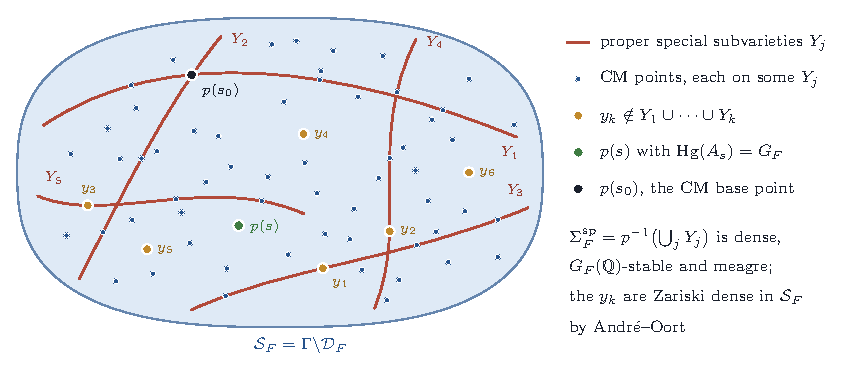
\includegraphics[width=\textwidth]{fig_speciallocus}
\caption{\Cref{prop:speciallocus} and \Cref{thm:escape} on the quotient
$\cS_{F}$. The curves are five of the countably many proper special
subvarieties $Y_{j}$, whose union is the image of the special locus; it
contains $p(s_{0})$ and is dense and meagre. The small dots are CM points,
each lying on some $Y_{j}$, drawn or not. The points $y_{1},\dots,y_{6}$
begin an escaping sequence chosen as in the proof of \Cref{thm:escape}(i):
$y_{k}$ lies on no $Y_{j}$ with $j\le k$, so $y_{1}$ may lie on $Y_{3}$ and
$y_{2}$ on $Y_{4}$. A point $p(s)$ at which the Hodge group is all of $G_{F}$
lies on none of them.}
\label{fig:speciallocus}
\end{figure}

\subsection{Weil tori of a CM field and the pure form}
\label{ssec:cmweiltori}

The argument of \Cref{thm:p2false} uses the field only through the
eigenspaces of its action, and it extends to every CM field. For $m\ge2$ the
Hodge ring of a very general Weil torus is larger than for an imaginary
quadratic field, since products of Weil classes over a set of embeddings
closed under conjugation are Hodge classes there, and a Weil torus may carry
subvarieties of codimension $2n$; but it carries none of codimension $n$, and
that is all the argument needs.

\begin{setupenv}[Weil tori of a CM field]\label{setup:cmweiltori}
Keep \Cref{setup:cmfield}, let $n\ge2$ and let $A$ be of $(F,n,\delta)$-Weil
type, with $V_{\CC}=\bigoplus_{\sigma}V_{\sigma}$ as there. Complex
conjugation carries $V_{\bbar\sigma}$ onto $V_{\sigma}$. A complex structure on
$V_{\RR}$ commuting with $F$, with $H^{1,0}\cap V_{\sigma}$ of dimension $n$
for every $\sigma$, is the same as a choice, for each real place $\tau$, of
complementary $n$-dimensional subspaces $X_{\tau},Y_{\tau}\subset
V_{\sigma_{\tau}}$: then $H^{1,0}\cap V_{\sigma_{\tau}}=X_{\tau}$,
$H^{0,1}\cap V_{\sigma_{\tau}}=Y_{\tau}$, and on $V_{\bbar\sigma_{\tau}}$ the
two parts are the conjugates of $Y_{\tau}$ and $X_{\tau}$. Call the complex
torus obtained in this way a Weil torus of $F$, and let $S_{F}$ be the
connected complex manifold of these choices, of dimension $2mn^{2}$. Its
tangent space at $A$ is $\Hom_{F}(H^{1,0},H^{0,1})$, the polarised family
$\cD_{F}$ is the submanifold on which $E$ is of type $(1,1)$, and $S_{F}$
contains non-algebraic tori. For $\sigma=\sigma_{\tau}$ the line
$\bigwedge^{2n}V_{\sigma}=\bigwedge^{n}X_{\tau}\otimes\bigwedge^{n}Y_{\tau}$ is
of type $(n,n)$, and likewise for $\bbar\sigma_{\tau}$, so $W_{F}$ consists
of Hodge classes on every member of $S_{F}$. For a set $\Sigma$ of
embeddings write $\alpha_{\Sigma}=\prod_{\sigma\in\Sigma}\alpha_{\sigma}$,
with $\alpha_{\sigma}$ spanning $\bigwedge^{2n}V_{\sigma}$.
\end{setupenv}

\begin{lemma}[Hodge classes and subvarieties of a very general Weil torus]
\label{lem:cmweiltori}
Let $T$ be a very general member of $S_{F}$ and $d=2mn=\dim T$.
\begin{enumerate}[label=\textup{(\roman*)},leftmargin=2.6em,itemsep=2pt]
\item Every Hodge class of $T$ lies in the span of the $\alpha_{\Sigma}$. In
  particular $\Hdg^{k}(T)=0$ unless $n$ divides $k$, and
  $\Hdg^{n}(T)=W_{F}(T)$.
\item Let $\kappa_{0}$ be the K\"ahler class of a hermitian form on the
  tangent space that is block diagonal for the splitting of $H^{1,0}$ into
  the $H^{1,0}\cap V_{\sigma}$. Then $\int_{T}\alpha_{\Sigma}\,
  \kappa_{0}^{\,d-n|\Sigma|}=0$ unless $\Sigma$ is closed under conjugation.
\item Every irreducible analytic subset of $T$ other than a point and $T$
  itself has codimension $ns$ with $s$ even, hence at least $2n$.
\end{enumerate}
\end{lemma}

\begin{proof}
(i) As in the proof of \Cref{lem:weiltorushodge}: a rational class of Hodge
type at a very general member is of Hodge type on all of $S_{F}$, and the
Mumford--Tate group $M$ of a very general member lies in
$G=\Res_{F/\QQ}\mathrm{GL}_{F}(V)$, since $F$ acts by endomorphisms. Here
$G(\RR)=\prod_{\tau}\mathrm{GL}(V_{\sigma_{\tau}})$ acts transitively on
$S_{F}$, and the $\mathrm{Ad}\,G(\RR)$-span of the complex structure of one
member is an ideal of $\bigoplus_{\tau}\mathfrak{gl}_{2n}(\CC)$ whose
projection to every factor contains a non-central element, $i$ on $X_{\tau}$
and $-i$ on $Y_{\tau}$. An ideal of a sum of simple real Lie algebras is a
sum of some of them, and each $\mathfrak{sl}_{2n}(\CC)$ is simple as a real
Lie algebra, so the span contains $\bigoplus_{\tau}\mathfrak{sl}_{2n}(\CC)$
and $M$ contains $\Res_{F/\QQ}\mathrm{SL}_{F}(V)$. Over $\CC$ this group is
$\prod_{\sigma}\mathrm{SL}(V_{\sigma})$ acting on
$\bigwedge^{*}V_{\CC}=\bigotimes_{\sigma}\bigwedge^{*}V_{\sigma}$, and the
invariants of $\mathrm{SL}(V_{\sigma})$ in $\bigwedge^{*}V_{\sigma}$ are
$\bigwedge^{0}$ and $\bigwedge^{2n}$. So the invariants are spanned by the
$\alpha_{\Sigma}$, of degree $2n|\Sigma|$, and a rational class in the span
of the $\alpha_{\sigma}$ lies in $W_{F}$.

(ii) Choose the hermitian form so that $\kappa_{0}=
\sqrt{-1}\sum_{\sigma}\sum_{k}\xi_{\sigma,k}\wedge\bbar\xi_{\sigma,k}$ with
$\xi_{\sigma,k}$ a basis of $H^{1,0}\cap V_{\sigma}$; each term lies in
$V_{\sigma}\otimes V_{\bbar\sigma}$. A product of classes has nonzero
integral only if its degree in every $V_{\rho}$ is $2n$. The factor
$\alpha_{\Sigma}$ has degree $2n$ in $V_{\rho}$ for $\rho\in\Sigma$ and $0$
otherwise, and every term of a power of $\kappa_{0}$ has the same degree in
$V_{\rho}$ as in $V_{\bbar\rho}$. For $\rho\in\Sigma$ that degree must be
$0$, so $V_{\bbar\rho}$ must be filled by $\alpha_{\Sigma}$, that is
$\bbar\rho\in\Sigma$.

(iii) Let $Z$ be irreducible of codimension $c$ with $0<c<d$. For a K\"ahler
class $\kappa$, $\int_{T}[Z]\,\kappa^{d-c}=\int_{Z}\kappa^{d-c}>0$, so $[Z]$ is
a nonzero Hodge class of degree $2c$, and by (i) $c=ns$ and $[Z]$ is a
combination of the $\alpha_{\Sigma}$ with $|\Sigma|=s$. Complex conjugation
permutes the embeddings without fixed points, so a set closed under it has
even size; if $s$ were odd, (ii) would give $\int_{T}[Z]\,\kappa_{0}^{d-c}=0$.
\end{proof}

\begin{proposition}[Coherent sheaves on a very general Weil torus of $F$]
\label{prop:cmweiltorussheaves}
Let $T$ be a very general member of $S_{F}$. Every coherent analytic sheaf
$\mathcal{F}$ on $T$ has $\ch_{k}(\mathcal{F})=0$ in $H^{2k}(T,\QQ)$ for
$1\le k\le2n-1$.
\end{proposition}

\begin{proof}
The Chern classes of \cite{Gri10} are Hodge classes, additive, and
compatible with restriction to open subsets, so by
\Cref{lem:cmweiltori}(i) only $k=n$ needs an argument. First let
$\mathcal{F}$ be supported on a proper analytic subset $W$. Its restriction to
$T\smallsetminus W$ is zero, so $\ch_{n}(\mathcal{F})$ comes from
$H^{2n}_{W}(T,\QQ)$, which is isomorphic to the Borel--Moore homology
$H_{2d-2n}(W,\QQ)$; by \Cref{lem:cmweiltori}(iii) every component of $W$ has
codimension at least $2n$, so $W$ has real dimension at most $2d-4n<2d-2n$
and that group vanishes. In general, the torsion of $\mathcal{F}$ is of this
kind, and so is the cokernel of the inclusion of a torsion-free sheaf in its
reflexive hull. Every coherent sheaf has $c_{1}=0$, since $\Hdg^{1}(T)=0$, so
as in the proof of \Cref{prop:weiltorussheaves} a torsion-free sheaf has a
Jordan--H\"older filtration whose factors $Q_{j}$ are stable for every
K\"ahler class, and $\ch_{n}(Q_{j})=\ch_{n}(Q_{j}^{**})$. By Bando and Siu
\cite{BS94}, $\int_{T}c_{2}(Q_{j}^{**})\,\kappa_{0}^{d-2}\ge0$, with equality
exactly when $Q_{j}^{**}$ is a projectively flat bundle. Here
$c_{2}(Q_{j}^{**})$ lies in $\Hdg^{2}(T)$, which is zero for $n\ge3$ and is
$W_{F}(T)$ for $n=2$, where the integral vanishes by
\Cref{lem:cmweiltori}(ii) with $|\Sigma|=1$. So $Q_{j}^{**}$ is projectively
flat with $c_{1}=0$, hence flat, and $\ch_{n}(Q_{j})=0$. Summing over the
factors and adding the torsion gives $\ch_{n}(\mathcal{F})=0$.
\end{proof}

\begin{theorem}[The pure form is never met, for any CM field]
\label{thm:cmpurefalse}
Let $n\ge2$, let $A$ be of $(F,n,\delta)$-Weil type, and let $E$ be a
perfect complex on $A$ whose Chern character stays of Hodge type on every
member of $S_{F}$ and has $\ch_{n}(E)\ne0$; for instance
$\ch(E)=c+N\omega$ with $c\in\QQ$, $N\ne0$ and $\omega$ a nonzero rational
Weil class. Then $\sigma_{E}$ is not injective, and
$\dim\Ext^{2}(E,E)>r(\ch E)$. In particular no complex of the pure form
$\ch(E)=N\omega_{s_{0}}$ in \Cref{thm:cmpropagation}(v), with or without a
rank, has injective semiregularity map, whatever the CM field.
\end{theorem}

\begin{proof}
The proof of \Cref{thm:p2false} applies with $S_{F}$ in place of $S$: an
injective $\sigma_{E}$ would let $E$ deform, by the theorem of Buchweitz and
Flenner in Pridham's form and Kuranishi's method, to a bounded complex of
holomorphic vector bundles on every member of a neighbourhood of $A$ in
$S_{F}$, with Chern character the parallel transport of $\ch(E)$; at a very
general member $\ch_{n}$ of that complex vanishes by
\Cref{prop:cmweiltorussheaves}, while it is the transport of
$\ch_{n}(E)\ne0$. A class $c+N\omega$ is of Hodge type on all of $S_{F}$ by
\Cref{setup:cmweiltori}. The inequality follows from the square
$\sigma_{E}\circ\operatorname{ev}_{E}=(\,\cdot\,)\lrcorner\ch(E)$, since
$\dim\Ext^{2}(E,E)\ge\operatorname{rk}\operatorname{ev}_{E}\ge r(\ch E)$ and
equality in both forces $\operatorname{ev}_{E}$ onto with kernel the
annihilator, and then $\sigma_{E}$ injective, as in
\Cref{thm:p2primenumber}(iv).
\end{proof}

For $m=1$ this is \Cref{thm:p2false}, and for $m=1$, $n=2$ the vanishing of
\Cref{prop:cmweiltorussheaves} is Voisin's theorem \cite[Theorem~10]{Voi02b}.
So the criterion of \Cref{thm:cmpropagation}(v) needs a polynomial $P$ in the
classes $\eta_{t}$ that is not constant, for every CM field and every
$n\ge2$. At a quartic field and $n=2$ this pushes the least possible value of
$\dim\Ext^{2}(E,E)$ for a complex meeting it from $80$ to $88$
(\Cref{cor:quarticleast}).

\subsection{Quartic CM fields at \texorpdfstring{$n=2$}{n=2}}
\label{ssec:quartic}

By \Cref{thm:closure}(ii) the only form of (P2) on a minimal route to the
conjecture is the one for the split families of the CM fields of degree at
least four, and by \Cref{prop:descent}(i) the Weil classes of any family of
such a field in a higher dimension give those of its families at $n=2$. For a
quartic field these are families of abelian eightfolds, the smallest
families of a field of degree at least four. This subsection determines how
far the available mechanisms reach there.

Divisor classes reach the Weil classes exactly on a Noether--Lefschetz locus,
which has codimension two when $\delta$ is trivial (\Cref{prop:quarticnl},
\Cref{cor:quarticbase}). For biquadratic $F$, Markman's theorem reaches them
on a further locus of dimension four (\Cref{prop:quarticscalar}). For
$F=\QQ(\zeta_{5}),\QQ(\zeta_{8}),\QQ(\zeta_{12})$ and trivial $\delta$,
Schoen's cycles on Prym varieties of cyclic covers reach them on a locus of
dimension at most six, at whose very general points the Hodge group is all of
$G_{F}$ (\Cref{rem:quarticprym}). The Casimir class of the quadratic form on
the weight two part $R_{F}$ below, the natural class of degree four attached
to it, is algebraic exactly when the Weil classes are
(\Cref{prop:quarticcasimir}), and correspondences with abelian varieties whose
simple factors have dimension at most seven cannot help at a member with full
Hodge group (\Cref{prop:quarticnogo}). For a general shape the polarised
criterion asks $\dim\Ext^{2}(E,E)=112$ of one complex
(\Cref{thm:quarticp2prime}). No Orlov product of sheaves on a principally
polarised fourfold with real multiplication meets the criterion through a
dimension count, whatever the quartic field (\Cref{thm:quarticobstruction}),
and no Orlov product of complexes does so unless both factors have nonzero self-Ext
groups in some degree at most $-3$ (\Cref{rem:quarticnegext}). Those products
are in any case candidates only for a twisted form of the criterion, the form
of Markman's reduction (\Cref{rem:quarticsecantshape}). Objects with pure
spinor characters give no Weil class at all (\Cref{prop:quarticexclusions}).
Together these results fix the loci that
divisors, scalar extension and correspondences reach inside $\cD_{F}$, and
the numbers that one complex has to attain on the rest.

Throughout, $F$ is a quartic CM field and $F_{0}$ its real quadratic subfield,
with real places $\tau_{1},\tau_{2}$, and $(V,H)$ is of $(F,2)$-Weil type with
discriminant $\delta$; so $m=n=2$, the members are abelian eightfolds, and
$\cD_{F}$ has dimension $mn^{2}=8$. By \Cref{prop:cmweil}(i),
$H^{1}(A,\CC)=\bigoplus_{\sigma}V_{\sigma}$ over the four embeddings $\sigma$ of
$F$, with $\dim V_{\sigma}^{1,0}=\dim V_{\sigma}^{0,1}=2$. Put
\[
  R_{F}=\textstyle\bigwedge^{2}_{F}V\;\subseteq\;\bigwedge^{2}_{\QQ}V=H^{2}(A,\QQ),
\]
the $\QQ$-subspace with complexification
$\bigoplus_{\sigma}\bigwedge^{2}V_{\sigma}$; for $m=1$ it is the space $R$ of
\Cref{prop:divfails}. It is an $F$-vector space of dimension $6$, of
$\QQ$-dimension $24$, with Hodge numbers $(4,16,4)$. Fix a generator $\Omega$
of the $F$-line $W_{F}=\bigwedge^{4}_{F}V$, so that
$W_{F}=\{a\Omega:a\in F\}$, and define a symmetric $F$-bilinear form $q$ on
$R_{F}$ by $x\wedge_{F}y=q(x,y)\,\Omega$. Let $h$ be the hermitian form on
$R_{F}$ induced by $H$, $h(x_{1}\wedge x_{2},y_{1}\wedge y_{2})
=\det\bigl(H(x_{i},y_{j})\bigr)$, and $h_{4}$ the one induced on
$\bigwedge^{4}_{F}V$; in a basis $e_{1},\dots,e_{4}$ with
$\Omega=e_{1}\wedge e_{2}\wedge e_{3}\wedge e_{4}$, $h_{4}(\Omega,\Omega)$ is
$\det H$, so its class in $F_{0}^{\times}/\Nm_{F/F_{0}}(F^{\times})$ is
$\delta$. With dual bases $(\omega_{k})$, $(\omega_{k}^{*})$ of $F$ for the
trace form, as in \Cref{thm:cmbasepoint}, put
$x\star y=\sum_{k}(\omega_{k}x)\cup(\omega_{k}^{*}y)$ for $x,y\in R_{F}$. Then
\begin{equation}\label{eq:quarticstar}
  x\star y=q(x,y)\,\Omega ,
\end{equation}
because the complexification of $(\omega_{k}x)\cup(\omega_{k}^{*}y)$ is
$\sum_{\sigma,\sigma'}\sigma(\omega_{k})\sigma'(\omega_{k}^{*})\,
x_{\sigma}\wedge y_{\sigma'}$, the sum over $k$ of the coefficient is $1$ for
$\sigma=\sigma'$ and $0$ otherwise, as in the proof of
\Cref{thm:cmbasepoint}(ii), and $\sum_{\sigma}x_{\sigma}\wedge y_{\sigma}$ is
the complexification of $q(x,y)\Omega$. Finally let $\theta_{j}\in H^{1,1}(A)$
be the component of the polarisation that pairs $V_{\sigma}$ with
$V_{\bbar\sigma}$ for the two embeddings $\sigma,\bbar\sigma$ over $\tau_{j}$.
Then $\eta_{t}=\sum_{j}\tau_{j}(t)\,\theta_{j}$ for the classes $\eta_{t}$ of
\Cref{prop:cmweil}(iii), and $\CC[\theta_{1},\theta_{2}]$ is the
complexification of the $\QQ$-algebra generated by the $\eta_{t}$.

\begin{proposition}[Hodge classes, and a quaternion algebra acting on $R_{F}$]
\label{prop:quarticquat}
Let $A$ be a member of an $(F,2,\delta)$-family.
\begin{enumerate}[label=\textup{(\roman*)},leftmargin=2.6em,itemsep=2pt]
\item If $\Hg(A)=G_{F}$, the space of Hodge classes of $A$ has dimension $2$
  in degree two, spanned by the $\eta_{t}$, and $7$ in degree four, spanned by
  the three products of two $\eta_{t}$ and by $W_{F}(A)$, which meets the span
  of those products in $0$.
\item The map $\phi\colon R_{F}\to R_{F}$ defined by $q(x,y)=h(x,\phi y)$
  satisfies $\phi(ax)=\bbar a\,\phi(x)$ for $a\in F$ and
  $\phi^{2}=h_{4}(\Omega,\Omega)^{-1}$, and it commutes with $\SU(V,H)$. So
  $\phi$ and the action of $F$ are Hodge endomorphisms of $R_{F}$ at every
  member, and the Hodge classes in $R_{F}$ form a module over the algebra
  $\cQ_{\delta}=F\oplus F\phi$.
\item $\cQ_{\delta}$ is the cyclic quaternion algebra $(F/F_{0},\delta)$ over
  $F_{0}$, which is split if and only if $\delta$ is trivial. If
  $\Hg(A)=G_{F}$, then $\cQ_{\delta}$ is the whole algebra of Hodge
  endomorphisms of $R_{F}$.
\item If $\delta$ is trivial, then $R_{F}=W\otimes_{F_{0}}F$ for a rational
  sub-Hodge structure $W$, stable under $F_{0}$, of dimension $12$ and with
  Hodge numbers $(2,8,2)$.
\end{enumerate}
\end{proposition}

\begin{proof}
(i) As in the proof of \Cref{prop:cmweil}(iii), over $\CC$ the group $G_{F}$
is $\SL(U_{1})\times\SL(U_{2})$ with $\dim U_{j}=4$, and
$H^{1}(A,\CC)=\bigoplus_{j}(U_{j}\oplus U_{j}^{\vee})$. The invariants of
$\SL(U)$ in $\bigwedge^{a}U\otimes\bigwedge^{b}U^{\vee}$ form a line if $a=b$
or $\{a,b\}=\{0,4\}$, and are zero otherwise. In degree two this leaves the
bidegree $(1,1)$ in one factor: two lines, spanned by $\theta_{1}$ and
$\theta_{2}$. In degree four it leaves $(2,2)$ in one factor or $(1,1)$ in
both, three lines spanned by $\theta_{1}^{2}$, $\theta_{1}\theta_{2}$ and
$\theta_{2}^{2}$, which are nonzero because $\dim U_{j}=4$; and $(4,0)$ or
$(0,4)$ in one factor, four lines spanning $W_{F}\otimes\CC$. These lie in
different summands, so $W_{F}(A)$ meets the span of the products in $0$.

(ii) Choose an $H$-orthogonal basis $e_{1},\dots,e_{4}$ of $V$ and put
$a_{i}=H(e_{i},e_{i})\in F_{0}$. Replacing $\Omega$ by $\lambda\Omega$
replaces $\phi$ by $\bbar\lambda^{-1}\phi$ and $h_{4}(\Omega,\Omega)$ by
$\Nm(\lambda)h_{4}(\Omega,\Omega)$, so we may take
$\Omega=e_{1}\wedge e_{2}\wedge e_{3}\wedge e_{4}$, with
$h_{4}(\Omega,\Omega)=a_{1}a_{2}a_{3}a_{4}$. For $J=\{j<j'\}$ put
$e_{J}=e_{j}\wedge e_{j'}$ and $a_{J}=a_{j}a_{j'}$, and let $J^{c}$ be the
complement, with $e_{J^{c}}\wedge e_{J}=\epsilon_{J}\Omega$. The $e_{J}$ form
an $h$-orthogonal $F$-basis with $h(e_{J},e_{J})=a_{J}$, and
$q(e_{K},e_{J})$ is $\epsilon_{J}$ for $K=J^{c}$ and $0$ otherwise, so
$\phi(e_{J})=\epsilon_{J}a_{J^{c}}^{-1}e_{J^{c}}$. Two-forms commute, so
$\epsilon_{J^{c}}=\epsilon_{J}$ and
$\phi^{2}(e_{J})=(a_{J}a_{J^{c}})^{-1}e_{J}=h_{4}(\Omega,\Omega)^{-1}e_{J}$.
Semilinearity holds because $q$ is linear and $h$ antilinear in the second
variable. An element of $\SU(V,H)$ preserves $h$ and fixes $\Omega$, hence
preserves $q$ and commutes with $\phi$, and it commutes with $F$. The Hodge
group of every member lies in $G_{F}$, because the circle defining the Hodge
structure preserves $E$, commutes with $F$ and acts on each $V_{\sigma}$ with
determinant $z^{2}z^{-2}=1$; so $\phi$ and $F$ commute with it, and they are
Hodge endomorphisms.

(iii) The relations $\phi a=\bbar a\phi$ and $\phi^{2}=h_{4}(\Omega,\Omega)^{-1}$
present $F\oplus F\phi$ as the cyclic algebra
$(F/F_{0},h_{4}(\Omega,\Omega)^{-1})$, which is $(F/F_{0},\delta)$ because a
square in $F_{0}$ is a norm; and a cyclic algebra $(F/F_{0},c)$ is split
exactly when $c$ is a norm from $F$. It has $\QQ$-dimension $8$, since $\phi$
is not $F$-linear. If $\Hg(A)=G_{F}$, the Hodge endomorphisms of $R_{F}$ are
the commutant of $G_{F}$. Over $\CC$,
$R_{F}\otimes\CC=\bigoplus_{j}\bigl(\bigwedge^{2}U_{j}\oplus
\bigwedge^{2}U_{j}^{\vee}\bigr)$, where
$\bigwedge^{2}U_{j}\cong\bigwedge^{2}U_{j}^{\vee}$ is irreducible for
$\SL(U_{j})$ and trivial for the other factor, so the commutant is
$M_{2}(\CC)\times M_{2}(\CC)$, of dimension $8$.

(iv) If $\delta$ is trivial, $h_{4}(\Omega,\Omega)=\Nm(b)$ for some $b\in F$,
and $\psi=b\phi$ satisfies $\psi^{2}=b\bbar b\,\phi^{2}=1$. Its fixed space
$W$ is an $F_{0}$-subspace and a sub-Hodge structure, $\psi$ being a Hodge
endomorphism, and an element $\beta\in F$ with $\bbar\beta=-\beta\ne0$ maps it
isomorphically onto the $(-1)$-eigenspace, since $\psi\beta=-\beta\psi$. So
$R_{F}=W\oplus\beta W=W\otimes_{F_{0}}F$, and $W$ has half the dimension and
half the Hodge numbers of $R_{F}$.
\end{proof}

\begin{proposition}[What divisor classes reach]\label{prop:quarticnl}
Let $A$ be a member of an $(F,2,\delta)$-family.
\begin{enumerate}[label=\textup{(\roman*)},leftmargin=2.6em,itemsep=2pt]
\item The following are equivalent: \textup{(a)} $W_{F}(A)$ lies in the
  subalgebra of $H^{*}(A,\QQ)$ generated by $\NS(A)_{\QQ}$; \textup{(b)}
  $W_{F}(A)$ meets that subalgebra in a nonzero class; \textup{(c)} $R_{F}$
  contains a nonzero rational Hodge class. When they hold, $R_{F}$ contains a
  rational Hodge class $t$ with $q(t,t)\ne0$, and
  $W_{F}(A)=\{(ft)\star t:f\in F\}$, a space of polynomials with rational
  coefficients in divisor classes.
\item For a nonzero $\cQ_{\delta}$-submodule $M\subseteq R_{F}$ let
  $\cD(M)\subseteq\cD_{F}$ be the set of points at which $M$ consists of Hodge
  classes, and let $\mathrm{NL}(R_{F})\subseteq\cD_{F}$ be the set of points at
  which \textup{(c)} holds. Then $\mathrm{NL}(R_{F})=\bigcup_{M}\cD(M)$, a
  countable union. Each nonempty $\cD(M)$ is a closed complex submanifold,
  isomorphic to a product of two bounded symmetric domains of type IV and
  dimension $4-d$ each, where $d=\dim_{F}M$, and $d=1$ occurs only if $\delta$ is
  trivial. So if $\delta$ is trivial, $\mathrm{NL}(R_{F})$ is the union of the
  nonempty $\cD(M)$ with $d=1$, each of dimension exactly $6$; if $\delta$ is
  not trivial, every $\cD(M)$ has dimension at most $4$.
\item $\mathrm{NL}(R_{F})$ contains the base point $s_{0}$ of
  \Cref{thm:cmbasepoint}, and for every $\delta$ it contains the locus of
  products $B_{1}\times B_{2}$ of two abelian fourfolds of $(F,1)$-Weil type,
  which has dimension $4$. The split locus, of members isogenous to
  $X\otimes_{\cO_{F_{0}}}\cO_{F}$ with $X$ an abelian fourfold with
  $F_{0}\subseteq\End^{0}(X)$, has dimension $6$, lies in the family of
  trivial discriminant, and is contained in $\mathrm{NL}(R_{F})$.
\end{enumerate}
\end{proposition}

\begin{proof}
(i) Since $W_{F}(A)\ne0$, (a) implies (b). Let $F^{\times}$ act on $H^{*}(A,\QQ)$ by
$\alpha\mapsto\iota(\alpha)^{*}$, which on
$\bigotimes_{\sigma}\bigwedge^{a_{\sigma}}V_{\sigma}$ is the character
$\prod_{\sigma}\sigma^{a_{\sigma}}$. The isotypic parts for the characters
$\sigma^{2}$ in degree two and $\sigma^{4}$ in degree four are $R_{F}$ and
$W_{F}$. The projections $p_{R}$ and $p_{W}$ onto them are rational, the two
sets of characters being Galois orbits, and they are morphisms of Hodge
structures, being $\QQ$-linear combinations of the $\iota(\alpha)^{*}$. The
characters occurring in $H^{2}$ are the products $\rho\rho'$, and the only way
to write $\sigma^{4}$ as a product of two of them is $\sigma^{2}\cdot\sigma^{2}$,
so $p_{W}(D\cup D')=q(p_{R}D,p_{R}D')\,\Omega$ for $D,D'\in H^{2}(A,\QQ)$. If a
nonzero $w\in W_{F}$ equals $\sum_{i}D_{i}\cup D_{i}'$ with
$D_{i},D_{i}'\in\NS(A)_{\QQ}$, then
$w=p_{W}(w)=\sum_{i}q(p_{R}D_{i},p_{R}D_{i}')\,\Omega$, so some $p_{R}D_{i}$ is
a nonzero rational Hodge class in $R_{F}$, and (b) implies (c). Conversely,
let $t\in R_{F}$ be a nonzero rational Hodge class. The part of type $(1,1)$
of $\bigwedge^{2}V_{\sigma}$ is $V_{\sigma}^{1,0}\wedge V_{\sigma}^{0,1}$, and
$H$ is definite of opposite signs on the two factors by \Cref{prop:cmweil}(i),
so $h$ is negative definite on it at each real place, and $h(t,t)\in F_{0}$ is
totally negative. By \Cref{prop:quarticquat}(ii),
$q(t,\phi t)=h(t,\phi^{2}t)=h_{4}(\Omega,\Omega)^{-1}h(t,t)\ne0$, so one of the
rational Hodge classes $t$, $\phi t$, $t+\phi t$, call it $t'$, has
$q(t',t')\ne0$. Each $\omega_{k}ft'$ and each $\omega_{k}^{*}t'$ is a rational
Hodge class in $H^{2}$, hence a divisor class, and by \eqref{eq:quarticstar}
$(ft')\star t'=f\,q(t',t')\,\Omega$, which runs over $W_{F}$ as $f$ runs over
$F$. So (c) implies (a), with the stated formula.

(ii) The Hodge classes in $R_{F}$ form a $\cQ_{\delta}$-module, so
$\mathrm{NL}(R_{F})$ is the union of the $\cD(M)$, and there are countably
many $M$. Fix a real place $\tau$, let $\sigma$ be an embedding over it, and
put $R_{\tau}=R_{F}\otimes_{F_{0},\tau}\RR$, a complex vector space of
dimension $6$ through $F\otimes_{F_{0},\tau}\RR=\CC$, identified with
$\bigwedge^{2}V_{\sigma}$. Since $\det H$ has sign $(-1)^{n}=1$ at $\tau$, the
map $\phi$ induces an antilinear $\phi_{\tau}$ on $R_{\tau}$ with
$\phi_{\tau}^{2}=\lambda^{2}$, $\lambda>0$. Its eigenspace
$W_{\tau}=\{x:\phi_{\tau}x=\lambda x\}$ is a real form of $R_{\tau}$ and a real
sub-Hodge structure with $W_{\tau}\otimes\CC\cong\bigwedge^{2}V_{\sigma}$, of
Hodge numbers $(1,4,1)$, on which $q=\lambda h$ is real of signature $(2,4)$,
positive on the plane $\Pi_{\tau}$ of real classes of type $(2,0)+(0,2)$ and
negative on those of type $(1,1)$. The group $\SU(V_{\tau},H_{\tau})$ acts on
$W_{\tau}$ preserving $q$, through the isogeny $\SU(2,2)\to\mathrm{SO}(2,4)^{0}$,
and the map from $\cD_{2,2}$ to the space of oriented positive planes in
$W_{\tau}$ that sends a point to $\Pi_{\tau}$ is the equivariant isomorphism of
the symmetric domains of this group onto one component,
$\cD^{\mathrm{IV}}(W_{\tau})$, of dimension $4$. For a quadratic space $P$ of
signature $(2,k)$ write likewise $\cD^{\mathrm{IV}}(P)$, of dimension $k$. Let
$M$ have $F$-dimension $d$. Then $M_{\tau}=M\otimes_{F_{0},\tau}\RR$ is stable
under $\phi$ and $F$, so $M_{\tau}=P_{\tau}\otimes\CC$ with
$P_{\tau}=M_{\tau}\cap W_{\tau}$ of real dimension $d$, and $M$ consists of
Hodge classes exactly when every $P_{\tau}$ is of type $(1,1)$, that is,
orthogonal to $\Pi_{\tau}$. So
$\cD(M)=\prod_{\tau}\cD^{\mathrm{IV}}(P_{\tau}^{\perp})$, which is empty unless
every $P_{\tau}$ is negative definite and then has dimension $2(4-d)$. If
$d=1$, then $M=Fx$ with $\phi x=bx$ for some $b\in F$, and
$\phi^{2}x=\bbar bb\,x$ gives $h_{4}(\Omega,\Omega)^{-1}=\Nm(b)$, so $\delta$ is
trivial. If $\delta$ is trivial, $\cQ_{\delta}\cong M_{2}(F_{0})$, every nonzero
module contains one with $d=1$, and $\cD(M)\subseteq\cD(M')$ for
$M'\subseteq M$.

(iii) The classes $\delta_{i}(f)$ of \Cref{thm:cmbasepoint}(ii) have
complexification in $\bigoplus_{\sigma}\bigwedge^{2}V_{\sigma}$, so they lie in
$R_{F}$, and they are Hodge classes at $s_{0}$. For a product,
$V=V_{1}\oplus V_{2}$ with $H$-orthogonal $F$-planes of signature $(1,1)$ at
each place, and $\bigwedge^{2}_{F}V_{1}\subseteq R_{F}$ is $W_{F}(B_{1})$, of
type $(1,1)$ by \Cref{prop:cmweil}(i). Every $\delta$ is the product of the
discriminants of two such planes, for instance of $\mathrm{diag}(1,-\delta)$
and $\mathrm{diag}(1,-1)$, and each factor varies in a family of dimension
$m=2$. On the split locus $H^{1}(A,\QQ)=U\otimes_{F_{0}}F$, with
$U=H^{1}(X,\QQ)$ and the complex structure of $X$ on the first factor. The
polarisation class $e$ of $X$ lies in $\bigwedge^{2}_{F_{0}}U$, the hermitian
form of $A$ is $c$ times the sesquilinear extension of the $F_{0}$-bilinear
form $e$, with $c\in F$ totally imaginary, and so $\det H=c^{4}\,\mathrm{Pf}(e)^{2}$
is a square in $F_{0}$ and $\delta$ is trivial. The class
$e\otimes1\in(\bigwedge^{2}_{F_{0}}U)\otimes_{F_{0}}F=R_{F}$ is fixed by
$\Hg(A)=\Hg(X)\subseteq\Res_{F_{0}/\QQ}\Sp(U,e)$, so it is a nonzero Hodge
class. The polarised abelian fourfolds with real multiplication by $F_{0}$
form families of dimension $[F_{0}:\QQ]\cdot3=6$.
\end{proof}

\begin{corollary}[A base locus of codimension two]\label{cor:quarticbase}
In every $(F,2,\delta)$-family, $\Sigma_{F}\supseteq\mathrm{NL}(R_{F})$, and at
every point of $\mathrm{NL}(R_{F})$ the Weil classes are the polynomials in
divisor classes of \Cref{prop:quarticnl}(i). If $\delta$ is trivial,
$\mathrm{NL}(R_{F})$ is a countable union of closed complex submanifolds of
$\cD_{F}$ of codimension exactly two, and it contains the split locus; if
$\delta$ is not trivial, they have codimension at least four, and the product
loci have codimension four. In both cases $\mathrm{NL}(R_{F})$ contains the
base point $s_{0}$ of \Cref{thm:cmbasepoint} and is stable under
$G_{F}(\QQ)$. At a point outside $\mathrm{NL}(R_{F})$ no nonzero Weil class is
a polynomial in divisor classes.
\end{corollary}

\begin{proof}
Everything except the stability is \Cref{prop:quarticnl}. An element
$g\in G_{F}(\QQ)$ commutes with $F$ and with $\phi$, so it carries
$\cQ_{\delta}$-submodules to $\cQ_{\delta}$-submodules, and
$g\,\cD(M)=\cD(gM)$.
\end{proof}

\Cref{thm:cmbasepoint} gives one CM point, whose $G_{F}(\QQ)$-orbit is dense
but countable. When $\delta$ is trivial, \Cref{cor:quarticbase} replaces it by
a locus of codimension two on which the Weil classes are balanced products of
divisor classes, as they are at $s_{0}$; nothing is claimed about the rest of
the Hodge ring at its points. It does not decide $\mathbf{W}(F,2,\delta)$:
$\mathrm{NL}(R_{F})$ is a countable union of proper closed submanifolds, hence
meagre, and \Cref{thm:cmpropagation}(iii) allows $\Sigma_{F}$ to be meagre.
The last sentence of the corollary is the analogue of \Cref{prop:divfails}:
no argument through divisor classes reaches a member outside
$\mathrm{NL}(R_{F})$. The codimension is two rather than
$h^{2,0}(R_{F})=4$ (compare \Cref{rem:nlcodim}) because Hodge classes in
$R_{F}$ come in $\cQ_{\delta}$-modules, and a module of $F$-dimension one costs
one condition at each real place. \Cref{fig:quarticloci} shows where the Weil
classes of such a family are known to be algebraic.

\begin{figure}[tbp]
\centering
  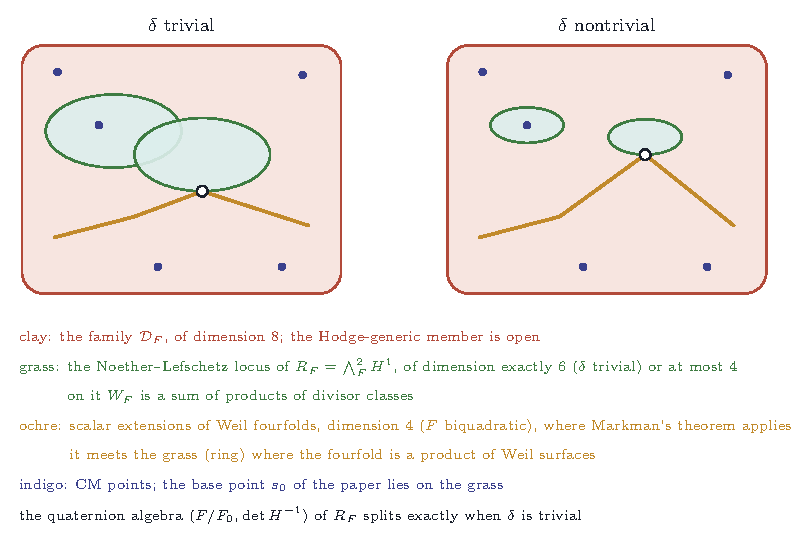
\includegraphics[width=0.94\textwidth]{fig_quarticloci}
\caption{Where the Weil classes of an $(F,2,\delta)$-family are known to be
algebraic, $F$ a quartic CM field; each panel is the period domain
$\cD_{F}$, of dimension $8$. The grass regions are components of the
Noether--Lefschetz locus $\mathrm{NL}(R_{F})$, on which $W_{F}$ consists of
polynomials in divisor classes (\Cref{prop:quarticnl},
\Cref{cor:quarticbase}): of dimension exactly $6$ when $\delta$ is trivial,
where the quaternion algebra $\cQ_{\delta}$ of \Cref{prop:quarticquat} is
split, and at most $4$ otherwise. The ochre curve is the locus of scalar
extensions of Weil fourfolds, of dimension $4$ when $F$ is biquadratic, on
which Markman's theorem applies (\Cref{prop:quarticscalar}); it is not
contained in $\mathrm{NL}(R_{F})$ but meets it (ring) where the fourfold is a
product of Weil surfaces. The indigo points are CM points; the base point
$s_{0}$ of \Cref{thm:cmbasepoint} lies on $\mathrm{NL}(R_{F})$. For
$F=\QQ(\zeta_{5}),\QQ(\zeta_{8}),\QQ(\zeta_{12})$ and trivial $\delta$ the Prym
locus of \Cref{rem:quarticprym}, of dimension at most $6$, is not drawn. On
the rest of the domain, the very general member included, the algebraicity
of the Weil classes is the open propagation statement.}
\label{fig:quarticloci}
\end{figure}

\begin{proposition}[Scalar extension from an imaginary quadratic subfield]
\label{prop:quarticscalar}
Let $F=KF_{0}$ with $K$ imaginary quadratic; these are the biquadratic
quartic CM fields, and the only ones containing an imaginary quadratic field.
Let $C$ be an abelian fourfold of $(K,2,\delta)$-Weil type and
$B_{F}=C\otimes_{\cO_{K}}\cO_{F}$, which is of $(F,2,\iota(\delta))$-Weil type by
\Cref{prop:descent}(ii); write $(V_{C},H_{C})$ for the hermitian space of $C$.
For $f\in F$ let $g_{f}\in\Hom(B_{F},C)\otimes\QQ$ be the element inducing
$v\mapsto v\otimes f$ from $H^{1}(C,\QQ)$ to
$H^{1}(B_{F},\QQ)=H^{1}(C,\QQ)\otimes_{K}F$.
\begin{enumerate}[label=\textup{(\roman*)},leftmargin=2.6em,itemsep=2pt]
\item $W_{F}(B_{F})$ lies in the $\QQ$-span of the classes $g_{f}^{*}w$, $f\in F$,
  $w\in W_{K}(C)$, which has dimension $10$. Hence $W_{F}(B_{F})$ is
  algebraic, by Markman's theorem $\mathbf{W}(K,2,\delta)$ \cite{Mar25a}
  (\Cref{prop:separate}(ii)).
\item The members $B_{F}$ form a locus of dimension $4$ in the
  $(F,2,\iota(\delta))$-family. At those with $\Hg(C)=\SU(V_{C},H_{C})$ the
  space $R_{F}$ contains no nonzero Hodge class, so
  this locus is not contained in $\mathrm{NL}(R_{F})$; it meets
  $\mathrm{NL}(R_{F})$, for instance where $C=C_{1}\times C_{2}$ with $C_{1}$,
  $C_{2}$ abelian surfaces of Weil type, and then $B_{F}$ is a product of two
  abelian fourfolds of $(F,1)$-Weil type.
\end{enumerate}
\end{proposition}

\begin{proof}
(i) The map $v\mapsto v\otimes f$ commutes with the complex structures, that of
$B_{F}$ being the one of $C$ tensored with $F$, so $g_{f}$ exists. Over $\CC$,
for each embedding $\kappa$ of $K$ let $V_{\kappa}$ be the $\kappa$-eigenspace
of $K$ on $H^{1}(C,\CC)$ and $U_{\kappa}=F\otimes_{K,\kappa}\CC\cong\CC^{2}$, the
sum of the lines $L_{\sigma}$, $\sigma|\kappa$, on which $F$ acts through
$\sigma$. The $\kappa$-part of $H^{1}(B_{F},\CC)$ is $V_{\kappa}\otimes
U_{\kappa}$ and its $\sigma$-part is $V_{\kappa}\otimes L_{\sigma}$, so the
$\sigma$-component $\bigwedge^{4}V_{\kappa}\otimes L_{\sigma}^{\otimes4}$ of
$W_{F}(B_{F})\otimes\CC$ lies in $\bigwedge^{4}V_{\kappa}\otimes
\mathrm{Sym}^{4}U_{\kappa}\subseteq\bigwedge^{4}(V_{\kappa}\otimes U_{\kappa})$.
The map $g_{f}^{*}$ sends a generator $\alpha_{\kappa}$ of $\bigwedge^{4}V_{\kappa}$
to $\alpha_{\kappa}\otimes f_{\kappa}^{\otimes4}$, with $f_{\kappa}$ the image
of $f$ in $U_{\kappa}$. The fourth powers of the elements of the Zariski
dense subset $F$ of $U_{\kappa}$ span $\mathrm{Sym}^{4}U_{\kappa}$, so the
complexified span of the $g_{f}^{*}w$ is $\bigoplus_{\kappa}\bigwedge^{4}V_{\kappa}
\otimes\mathrm{Sym}^{4}U_{\kappa}$, of dimension $2\cdot5$, and it contains
$W_{F}(B_{F})\otimes\CC$. A rational subspace whose complexification lies in
that of a rational subspace lies in it, and pull-backs of algebraic classes
are algebraic.

(ii) The map $C\mapsto B_{F}$ embeds the four-dimensional domain of the
$K$-family into $\cD_{F}$. As rational Hodge structures
$H^{1}(B_{F},\QQ)\cong H^{1}(C,\QQ)^{2}$, so $\Hg(B_{F})=\Hg(C)$, and
$R_{F}\otimes\CC=\bigoplus_{\sigma}\bigwedge^{2}V_{\kappa}\otimes
L_{\sigma}^{\otimes2}$, with $\bigwedge^{2}V_{\kappa}$ irreducible and
nontrivial for $\SL(V_{\kappa})$; so when $\Hg(C)=\SU(V_{C},H_{C})$, $R_{F}$
has no invariants. For $C=C_{1}\times C_{2}$ one has
$B_{F}=(C_{1}\otimes_{\cO_{K}}\cO_{F})\times(C_{2}\otimes_{\cO_{K}}\cO_{F})$, and
\Cref{prop:quarticnl}(iii) applies.
\end{proof}

\Cref{prop:quarticscalar} gives no new case of the Hodge conjecture: $B_{F}$ is
isogenous to $C\times C$, the classes are Hodge classes there, and when
$\Hg(C)=\SU(V_{C},H_{C})$ \Cref{prop:powers} already gives the conjecture for
$C\times C$ from \cite{Mar25a}.

\begin{remark}[Prym varieties of cyclic covers]\label{rem:quarticprym}
For three cyclotomic fields published work gives a further locus, at whose
very general points the Hodge group is the whole of $G_{F}$. Let $N\ge3$,
let $\widetilde C\to C$ be an \'etale cyclic cover of degree $N$ of a smooth
projective curve of genus
$g\ge2$, and let $P\subseteq J(\widetilde C)$ be the abelian subvariety on
whose $H^{1}$ the covering group acts through characters of exact order $N$.
Then $F=\QQ(\zeta_{N})$ acts on $P$, and every embedding of $F$ occurs in
$H^{1,0}(P)$ with multiplicity $g-1$ \cite[Lemma~1.6a]{Sch88},
\cite[Lemma~5.1]{PZ25}, so $P$ is of $(F,g-1)$-Weil type
(\Cref{rem:cmmember}). The hermitian form is split, because the part of
$H_{1}(\widetilde C,\ZZ)$ on which the covering group acts through
characters of exact order $N$ has a hyperbolic $\ZZ[\zeta_{N}]$-basis
\cite[Proposition~2.2]{Loo97}; so $\delta=[(-1)^{g-1}]$, which is trivial for
$g=3$. Schoen proved that the Weil classes of $P$ are algebraic
\cite[Theorem~2.0 with $r=0$, Corollary~3.1]{Sch88}, and Patel and Zhang give
a proof by unramified geometric class field theory
\cite[Theorems~1.1, 1.2 and~5.3, Remark~3.7]{PZ25}. By
\cite[Theorem~2.4]{Loo97}, for every $g\ge2$, the monodromy group of the
family of the $P$ over a finite cover of the moduli of such covers contains a
subgroup of finite index of an arithmetic subgroup of $G_{F}$. Every factor
$\SU(g-1,g-1)$ of $G_{F}(\RR)$ is noncompact, so by Borel's density theorem
\cite{Bor60} its Zariski closure contains $G_{F}$; the Hodge group of every
member lies in $G_{F}$, so by Andr\'e's theorem \cite[Theorem~1]{And92} a very
general $P$ has $\Hg(P)=G_{F}$, and by \Cref{prop:cmweil}(iii) the Hodge
conjecture holds for it in every degree. All of this is a consequence of
\cite{Sch88,Loo97,And92}, and we make no claim of priority.

For $\varphi(N)=4$, that is for $F=\QQ(\zeta_{5})=\QQ(\zeta_{10})$,
$\QQ(\zeta_{8})$ and $\QQ(\zeta_{12})$, and $g=3$, the $P$ are abelian
eightfolds of $(F,2,1)$-Weil type. With their $G_{F}(\QQ)$-translates, which
lie in $\Sigma_{F}$ by \Cref{thm:cmpropagation}(ii), they fill a countable
union of analytic subvarieties of $\cD_{F}$, the \emph{Prym locus} of $F$, of
positive dimension, since the monodromy is infinite, and of dimension at most
$3g-3=6$ \cite[pp.~25--26]{Sch88}. At a very general point of it $\Hg=G_{F}$, so
$R_{F}$ has no nonzero Hodge class there, each $\bigwedge^{2}V_{\sigma}$ being
a nontrivial irreducible representation of $\SL(V_{\sigma})$, and the Hodge
group is larger than that of a scalar extension of a Weil fourfold: such
points lie outside $\mathrm{NL}(R_{F})$, outside the locus of
\Cref{prop:quarticscalar}, and are not CM points. They are the only members
with $\Hg=G_{F}$ at which we know the Weil classes of a quartic CM field to be
algebraic. They do not decide $\mathbf{W}(F,2,1)$: the count
$3g-3=6<8=\tfrac12\varphi(N)(g-1)^{2}=\dim\cD_{F}$ of \cite[pp.~25--26]{Sch88}
makes the union meagre, as $\mathrm{NL}(R_{F})$ is, and
\Cref{thm:cmpropagation}(iii) allows $\Sigma_{F}$ to be meagre. Nor does
\Cref{prop:quarticnogo} exclude them: the cycles come from $J(\widetilde C)$,
which has $P$ as a factor. For imaginary quadratic fields the count is
$3n\ge n^{2}$ for $n\le3$, and there the Prym varieties do reach whole
families: Schoen proved the algebraicity for the Weil fourfolds and for a
family of Weil sixfolds of $\QQ(\sqrt{-3})$ \cite[Theorem~3.2]{Sch88},
\cite{Sch98}, and Koike for a family of Weil sixfolds of $\QQ(\sqrt{-1})$
\cite[Theorem~2.1, Corollary~2.1]{Koi04}.
\end{remark}

\begin{proposition}[The Casimir class]\label{prop:quarticcasimir}
Let $A$ be a member of an $(F,2,\delta)$-family and $c\in F^{\times}$, and let
\[
  C_{q}\in R_{F}\otimes_{\QQ}R_{F}\subseteq H^{2}(A,\QQ)\otimes H^{2}(A,\QQ)
  \subseteq H^{4}(A\times A,\QQ)
\]
be the Casimir element $\sum_{j}u_{j}\otimes u_{j}^{*}$ of the nondegenerate
symmetric form $\Tr_{F/\QQ}(c^{-1}q)$ on $R_{F}$, for a basis $(u_{j})$ and its
dual basis $(u_{j}^{*})$. Then $C_{q}$ is a Hodge class,
$\Delta^{*}C_{q}=6c\,\Omega$ for the diagonal $\Delta\colon A\to A\times A$,
and $C_{q}$ lies in the $\QQ$-span of the classes $f^{*}w$, $w\in W_{F}(A)$,
$f(x,y)=\iota(a)x+\iota(b)y$ with $a,b\in\cO_{F}$. Hence $W_{F}(A)$ is
algebraic if and only if $C_{q}$ is.
\end{proposition}

\begin{proof}
For an $F$-basis $(x_{I})$ of $R_{F}$ and its $q$-dual basis $(x_{I}^{q})$, the
elements $\omega_{k}x_{I}$ and $c\,\omega_{k}^{*}x_{I}^{q}$ form dual bases for
$\Tr_{F/\QQ}(c^{-1}q)$. So by \eqref{eq:quarticstar}
$\Delta^{*}C_{q}=\sum_{I}x_{I}\star(c\,x_{I}^{q})=\sum_{I}c\,\Omega=6c\,\Omega$,
and if $C_{q}$ is algebraic so is $W_{F}(A)$, by \Cref{prop:cmweil}(ii).
Conversely, $\SU(V,H)$ preserves $q$, so $C_{q}$ is invariant under the
diagonal action of $G_{F}$, which contains $\Hg(A\times A)$, and $C_{q}$ is a
Hodge class. Since $q$ pairs $\bigwedge^{2}V_{\sigma}$ only with itself, the
complexification of $C_{q}$ lies in $\bigoplus_{\sigma}\bigwedge^{2}V_{\sigma}
\otimes\bigwedge^{2}V_{\sigma}$, inside the part
$\bigoplus_{\sigma}\bigwedge^{4}(V_{\sigma}\otimes\CC^{2})$ of
$H^{4}(A\times A,\CC)$ on which $F^{\times}$, acting diagonally, has the
characters $\sigma^{4}$. The group $G_{F}$ acts on $V_{\sigma}$ through
$\SL(V_{\sigma})$, whose invariants in $\bigwedge^{4}(V_{\sigma}\otimes\CC^{2})$
are $\bigwedge^{4}V_{\sigma}\otimes\mathrm{Sym}^{4}\CC^{2}$ by Cauchy's
formula, so the $G_{F}$-invariants in that part form the rational space
$W_{F}(A)\otimes_{F}\mathrm{Sym}^{4}_{F}(F^{2})$, of dimension $20$. The map
$f^{*}$ sends $w$ to $w\otimes(a,b)^{\otimes4}$, and the fourth powers of the
elements of $\cO_{F}^{2}$ span $\mathrm{Sym}^{4}_{F}(F^{2})$; so the classes
$f^{*}w$ span that space, and $C_{q}$ is algebraic if $W_{F}(A)$ is.
\end{proof}

\begin{remark}[What the exceptional isogeny gives]\label{rem:quarticisogeny}
By the proof of \Cref{prop:quarticnl}(ii), at each real place $R_{F}$ becomes
$W_{\tau}\otimes\CC$ with $W_{\tau}$ of K3 type, $\SU(V_{\tau},H_{\tau})$ acting
through $\SU(2,2)\to\mathrm{SO}(2,4)$, and when $\delta$ is trivial the
$W_{\tau}$ are the real components of the rational structure $W$ of
\Cref{prop:quarticquat}(iv). A route of Kuga--Satake type would start from
this weight two structure and would have to return to degree four, on $A$ or
on $A\times A$; by \Cref{prop:quarticcasimir} the natural class it meets
there, the Casimir class of $q$, is algebraic exactly when the Weil classes
are. So this mechanism restates $\mathbf{W}(F,2,\delta)$ at each member and
does not reduce it.
\end{remark}

\begin{proposition}[No correspondence from a small abelian variety]
\label{prop:quarticnogo}
Let $A$ be a member with $\Hg(A)=G_{F}$, and let $X$ be an abelian variety
such that $\Hg(X)$ has no normal subgroup isogenous to $G_{F}$; by the proof,
this holds when every simple factor of $X$ has dimension at most $7$, in
particular when $\dim X\le7$, and it holds when $X$ is of CM type. Then
$\Hg(A\times X)=\Hg(A)\times\Hg(X)$, and
$\Hdg^{*}(A^{a}\times X^{b})=\Hdg^{*}(A^{a})\otimes\Hdg^{*}(X^{b})$ for all
$a,b\ge0$. So the class of an algebraic cycle $Z$ on $A^{a}\times X^{b}$ is
$\sum_{i}\beta_{i}\otimes\xi_{i}$ with $\beta_{i}\in\Hdg^{*}(A^{a})$ and
linearly independent $\xi_{i}\in\Hdg^{*}(X^{b})$; the correspondence $Z$
carries $H^{*}(X^{b},\QQ)$ into the span of the $\beta_{i}$; and if the Hodge
conjecture holds for $X^{b}$, every $\beta_{i}$ is algebraic.
\end{proposition}

\begin{proof}
The group $G_{F}=\Res_{F_{0}/\QQ}\SU(V,H)$ is almost simple over $\QQ$. By
Goursat's lemma the kernel $N$ of the projection $\Hg(A\times X)\to\Hg(X)$
maps onto a normal subgroup of $\Hg(A)=G_{F}$. If that subgroup is $G_{F}$,
then $\Hg(A\times X)$ contains $G_{F}\times1$ and is the product. Otherwise
$N$ is finite, $\Hg(X)$ has a normal subgroup $H$ isogenous to $G_{F}$,
contrary to the hypothesis, and the cocharacter $\mu$ defining the Hodge
structure of $X$ projects through $H\to G_{F}$ to that of $A$. This situation
also cannot occur when every simple factor of $X$ has dimension at most $7$,
or when $X$ is of CM type, as follows. Over $\CC$, $H$ is $\SL_{4}\times\SL_{4}$,
and $\mu$ projects in each factor to
$\mathrm{diag}(\frac12,\frac12,-\frac12,-\frac12)$ modulo the centre. Since
$\mu$ acts on $H^{1}(X,\CC)$ with two weights differing by one, the weights of
its projection spread by at most one on every irreducible constituent for
$H$; for the representation of $\SL_{4}$ of highest weight
$a\varpi_{1}+b\varpi_{2}+c\varpi_{3}$ the spread is $a+2b+c$, and spreads add
over the two factors. So every nontrivial constituent is the standard
representation of one factor or its dual. These four are permuted
transitively by $\Gal(\bbar\QQ/\QQ)$, as the embeddings of $F$ are; so a simple
factor $Y$ of $X$ on whose $H^{1}$ the group $H$ acts nontrivially has
$\dim_{\QQ}H^{1}(Y,\QQ)\ge16$, that is $\dim Y\ge8$. A torus has no such $H$.
Next, $\Hg(A^{a}\times X^{b})$ is $\Hg(A)\times\Hg(X)$ acting factorwise on
$H^{*}(A^{a})\otimes H^{*}(X^{b})$, and the invariants of a product of groups
in a tensor product of representations of the factors are the tensor product
of the invariants. Finally, the intersection pairing is perfect on
$\Hdg^{*}(X^{b})$, the invariants being orthogonal to the other isotypic
parts, so there are $\xi_{j}^{*}\in\Hdg^{*}(X^{b})$ with
$\int\xi_{i}\xi_{j}^{*}=\delta_{ij}$; they are algebraic when the conjecture
holds for $X^{b}$, and then $\beta_{j}=pr_{A^{a}*}(Z\cdot pr_{X^{b}}^{*}\xi_{j}^{*})$
is algebraic.
\end{proof}

So a correspondence with such an $X$ can produce a Weil class of $A$ only from
an algebraic cycle on some $A^{a}\times X^{b}$ that already yields one on
$A^{a}$. At a member with full Hodge group this excludes every abelian
variety of dimension at most seven, among them the fourfolds and sixfolds of
Weil type of the imaginary quadratic fields on which Markman's theorems are
proved, and every CM abelian variety. The same argument, with real points in
place of dimensions, excludes rational Hodge structures $Y$ of K3 type: by
Zarhin's theorem \cite{Zar83} the Hodge group of such a $Y$ is the restriction
of scalars of an orthogonal or unitary group over the endomorphism field of
its transcendental part, noncompact at exactly one real place, so its real Lie
algebra has at most one simple factor isomorphic to $\mathfrak{su}(2,2)$,
while that of $G_{F}$ has two; hence $\Hg(A\times Y)=\Hg(A)\times\Hg(Y)$.
This last statement rests on Zarhin's theorem, which we quote without proof.

\begin{theorem}[The polarised criterion for a quartic field at $n=2$]
\label{thm:quarticp2prime}
Let $A$ be a member of an $(F,2,\delta)$-family, let
$\omega=\sum_{\sigma}u_{\sigma}\alpha_{\sigma}$, with $\alpha_{\sigma}$ spanning
$\bigwedge^{4}V_{\sigma}$ and every $u_{\sigma}\ne0$, as holds for every
nonzero rational Weil class, let $p\in\CC[\theta_{1},\theta_{2}]$, put
$\gamma=\omega+p$, and let $r(\gamma)$ be the rank of the contraction
$HT^{2}(A)\to H^{*}(A,\CC)$, $\xi\mapsto\xi\lrcorner\gamma$. Write
$T_{\sigma}=(V_{\sigma}^{1,0})^{\vee}\subseteq T_{0}A$.
\begin{enumerate}[label=\textup{(\roman*)},leftmargin=2.6em,itemsep=2pt]
\item $\dim HT^{2}(A)=28+64+28=120$, and
  \[
    \Ann_{HT^{2}}(\omega)=\textstyle\bigoplus_{\sigma}
    \Hom\bigl(V_{\sigma}^{1,0},V_{\sigma}^{0,1}\bigr)\;\oplus\;
    \bigoplus_{\{\sigma,\sigma'\},\,\sigma\ne\sigma'}T_{\sigma}\otimes T_{\sigma'},
  \]
  of dimension $0+16+24$: the $F$-linear first order deformations of $A$ and
  the bivectors mixing two embeddings. So $r(\omega)=80$. Unlike the case
  $m=1$ of \Cref{thm:p2forces}(i), no nonzero element of $H^{0,2}(A)$ kills
  $\omega$.
\item $r(\gamma)\le112$ for every $p$. For a general $p$, $r(\gamma)=112$, and
  whenever $r(\gamma)=112$ the annihilator of $\gamma$ is the tangent space
  $T_{[A]}\cD_{F}$ of the family, of dimension $8$, inside $H^{1}(T_{A})$. The
  value $112$ is also taken at a general element, with nonzero component in
  $W_{F}\otimes\CC$, of the complexified Hodge ring of a member with
  $\Hg(A)=G_{F}$.
\item $r(\gamma)\ge80$ for every $p$, with equality exactly when $p$ is a
  constant.
\item The rank $r(\gamma)$ takes exactly the fifteen values $80$, $84$, $87$,
  $88$, $91$, $92$, $94$, $95$, $96$, $104$, $107$, $108$, $110$, $111$,
  $112$; \Cref{thm:quarticrank} computes it for every $p$. On the monomials
  $\theta_{1}^{i}\theta_{2}^{j}$ with a general coefficient it takes the
  six values $80$, $84$, $88$, $104$, $108$, $112$.
\item Let $E$ be a perfect complex on $A$ with $\ch(E)=N\omega_{1}+P$, where
  $N\ne0$, $\omega_{1}$ is a nonzero rational Weil class and $P$ is a
  polynomial with rational coefficients in the classes $\eta_{t}$. Then
  $\dim\Ext^{2}(E,E)\ge r(\ch E)\ge80$. If $\dim\Ext^{2}(E,E)=r(\ch E)$, then
  $\operatorname{ev}_{E}$ is onto with kernel $\Ann_{HT^{2}}(\ch E)$ and
  $\sigma_{E}$ is injective, so that $\mathbf{W}(F,2,\delta)$ follows by
  \Cref{thm:cmpropagation}(v).
\end{enumerate}
\end{theorem}

\begin{proof}
(i) $HT^{2}(A)=\bigwedge^{2}H^{0,1}\oplus H^{0,1}\otimes T_{0}A\oplus
\bigwedge^{2}T_{0}A$, with $H^{0,1}$ and $T_{0}A$ of dimension $8$. As in the
proof of \Cref{thm:p2forces}(i) the three summands map into different Hodge
components, so the annihilator is the sum of the three annihilators; and the
torus $(\CC^{\times})^{4}$ acting on each $V_{\sigma}$ by scalars separates the
images further. A block $V_{\rho}^{0,1}\wedge V_{\rho'}^{0,1}$ of
$\bigwedge^{2}H^{0,1}$ kills $\alpha_{\sigma}$ exactly when
$\sigma\in\{\rho,\rho'\}$, and otherwise maps injectively into a weight space
that no other pair of a block and an embedding reaches; there are four
embeddings, so some $\sigma$ lies outside $\{\rho,\rho'\}$, and no nonzero
element of $\bigwedge^{2}H^{0,1}$ kills $\omega$. A block
$\Hom(V_{\rho}^{1,0},V_{\rho'}^{0,1})$ of $H^{1}(T_{A})$ kills $\alpha_{\sigma}$
for $\sigma\ne\rho$; it kills $\alpha_{\rho}$ when $\rho'=\rho$, because
$V_{\rho}^{0,1}$ is already exhausted in $\alpha_{\rho}$, and maps it
injectively into its own weight space when $\rho'\ne\rho$. A bivector in
$T_{\rho}\otimes T_{\rho'}$ with $\rho\ne\rho'$ kills every $\alpha_{\sigma}$,
whose two factors of type $(1,0)$ both lie in $V_{\sigma}^{1,0}$, and
$\bigwedge^{2}T_{\sigma}$ maps $\alpha_{\sigma}$ to a nonzero multiple of a
generator of $\bigwedge^{2}V_{\sigma}^{0,1}$. The dimensions are $0$,
$4\cdot4$ and $6\cdot4$.

(ii) The classes $\theta_{j}$ and the rational Weil classes stay of Hodge type
along $\cD_{F}$, so each is killed by $T_{[A]}\cD_{F}\subseteq H^{1}(T_{A})$, as
in \Cref{prop:p2primelocus}(i); hence $r(\gamma)\le120-8$, and when equality
holds the annihilator, of dimension $8$, is $T_{[A]}\cD_{F}$. Take a basis of
$H^{1}(A,\CC)$ adapted to the $V_{\sigma}$ and to the Hodge decomposition, in
which the polarisation pairs the basis of $V_{\sigma}^{1,0}$ with that of
$V_{\bbar\sigma}^{0,1}$. The torus acting diagonally on it contains a subtorus
that multiplies each $\theta_{j}$ by a scalar and each $\alpha_{\sigma}$ by an
arbitrary scalar, and contraction is equivariant; so $r(\omega+p)$ depends on
$\omega$ only through a rescaling of the variables of $p$, and each statement
of the theorem holds for every $\omega$ once it holds for one. The rank is
lower semicontinuous in $p$, and it equals $112$ at
$p=\theta_{1}^{2}\theta_{2}^{2}$ by \Cref{thm:quarticrank}(iii) below, so it
equals $112$ for a general $p$. Every element of the complexified Hodge ring
of a member with $\Hg(A)=G_{F}$ is invariant under $G_{F}$, so its components
stay of Hodge type along $\cD_{F}$ and it is killed by $T_{[A]}\cD_{F}$; its
rank is therefore at most $112$. The ring contains $\omega+\theta_{1}^{2}
\theta_{2}^{2}$, since it contains $W_{F}\otimes\CC$ and the classes
$\theta_{1}$, $\theta_{2}$, whose span is defined over $\QQ$, and the rank
is lower semicontinuous; so it is $112$ at a general element of the ring, whose
component in $W_{F}\otimes\CC$ is not zero.

(iii) and (iv) are \Cref{thm:quarticrank}(iii) and (iv) below.

(v) By the commutative square $\sigma_{E}\circ\operatorname{ev}_{E}=(\,\cdot\,)
\lrcorner\ch(E)$ of \Cref{setup:criterion}, which holds on every abelian
variety, $\dim\Ext^{2}(E,E)\ge\operatorname{rk}\operatorname{ev}_{E}\ge
r(\ch E)$, and equality forces $\operatorname{ev}_{E}$ to be onto with kernel
the annihilator and $\sigma_{E}$ to be injective, as in
\Cref{thm:p2primenumber}(iv); and $r(\ch E)\ge80$ by (iii), since the
complexification of $\ch(E)$ is a $\gamma$ as above with $\omega=N\omega_{1}$.
The last implication is \Cref{thm:cmpropagation}(v), whose character is
exactly of this form.
\end{proof}

At $m=1$ and $n=2$ the corresponding numbers are $28$, $12$ and $24$
(\Cref{thm:p2primenumber}); in both cases the general value is the dimension
of $HT^{2}$ minus that of the family. For the pure shape the argument of
\Cref{thm:p2forces}(ii) and (iv) transfers with the annihilator of
\Cref{thm:quarticp2prime}(i): an injective $\sigma_{E}$ would force
$A_{\theta}A_{\theta'}=0$ for $\theta\in T_{\rho}$, $\theta'\in T_{\rho'}$,
$\rho\ne\rho'$, and a smooth component of the support of codimension at least
two along which $E$ is locally free of positive rank would be tangent to three
of the four $T_{\rho}$. The pure shape is excluded, for every CM
field, by \Cref{thm:cmpurefalse}.

The rank $r(\gamma)$ can be computed for every $p$. In the basis of the
proof of \Cref{thm:quarticp2prime}(ii) write $x_{\sigma,1},x_{\sigma,2}$ for
the basis of $V_{\sigma}^{1,0}$, $y_{\sigma,1},y_{\sigma,2}$ for that of
$V_{\sigma}^{0,1}$, and $\partial_{\sigma,1},\partial_{\sigma,2}$ for the dual
basis of $T_{\sigma}$, so that $\theta_{j}=\sum_{\sigma|\tau_{j}}\sum_{k}
x_{\sigma,k}\,y_{\bbar\sigma,k}$ and $\alpha_{\sigma}=x_{\sigma,1}x_{\sigma,2}
y_{\sigma,1}y_{\sigma,2}$, and use the torus of that proof to make every
$u_{\sigma}$ equal to $1$. Expand
$p=\sum_{i,j=0}^{4}e_{ij}\,\theta_{1}^{i}\theta_{2}^{j}/(i!\,j!)$, so that
$e_{ij}$ is a derivative of $p$ at $0$, and put:
\begin{itemize}[leftmargin=1.6em,itemsep=1pt]
\item $\mu(p)=0$ if $\partial_{1}\partial_{2}p=0$ and $\mu(p)=1$ otherwise,
  the derivatives taken in $\CC[\theta_{1},\theta_{2}]$;
\item $\rho_{1}(p)$ the dimension of the span of $\partial_{1}p$ and
  $\partial_{1}^{2}p$ modulo $\theta_{1}^{3}$, which is the rank of the
  $2\times15$ matrix whose columns are the pairs $(e_{i,j},e_{i+1,j})$,
  $1\le i\le3$, $0\le j\le4$; and $\rho_{2}(p)$ likewise, with the two indices
  exchanged;
\item for $t=1,2$, with $\sigma,\bbar\sigma$ the embeddings over $\tau_{t}$,
  $W_{t}\subseteq HT^{2}(A)$ the span of the eight elements
  $y_{\sigma,1}\wedge y_{\sigma,2}$, $y_{\bbar\sigma,1}\wedge
  y_{\bbar\sigma,2}$, $\partial_{\sigma,1}\wedge\partial_{\sigma,2}$,
  $\partial_{\bbar\sigma,1}\wedge\partial_{\bbar\sigma,2}$ and
  $y_{\sigma,k}\otimes\partial_{\bbar\sigma,l}$,
  $y_{\bbar\sigma,k}\otimes\partial_{\sigma,l}$ with $k\ne l$, and $R_{t}(p)$
  the rank of $\xi\mapsto\xi\lrcorner\gamma$ on $W_{t}$;
\item $h_{1}=e_{1}e_{3}-e_{2}^{2}$, $h_{2}=e_{2}e_{4}-e_{3}^{2}$,
  $h_{3}=e_{1}e_{4}-e_{2}e_{3}$ on $\CC^{4}$, and $V_{\pm}\subset\CC^{4}$ the
  set where $h_{3}=\pm e_{3}$, $2h_{2}=\pm e_{4}$ and $2h_{1}+1=\pm e_{2}$.
\end{itemize}

\begin{theorem}[The rank of the criterion at a quartic field]
\label{thm:quarticrank}
In this notation:
\begin{enumerate}[label=\textup{(\roman*)},leftmargin=2.6em,itemsep=2pt]
\item $r(\gamma)=64+16\mu(p)+4\rho_{1}(p)+4\rho_{2}(p)+R_{1}(p)+R_{2}(p)$.
\item $R_{t}(p)\in\{7,8\}$. If $R_{1}(p)=7$, then
  $(e_{10},e_{20},e_{30},e_{40})$ lies on $V_{+}\cup V_{-}$ and
  $\rho_{1}(p)=2$; conversely, if $\mu(p)=0$ and
  $(e_{10},\dots,e_{40})$ lies on $V_{+}\cup V_{-}$, then $R_{1}(p)=7$, as for
  $p=\theta_{1}^{2}/2$. The same holds for $R_{2}$ with
  $(e_{01},\dots,e_{04})$. Each $V_{\pm}$ contains the surface of points
  $(w\lambda\pm\frac{3}{2\lambda},\,w\lambda^{2}\pm\frac12,\,w\lambda^{3},
  \,w\lambda^{4})$, $w\in\CC$, $\lambda\in\CC^{\times}$.
\item $r(\gamma)\ge80$, with equality exactly when $p$ is a constant, and
  $r(\gamma)$ takes exactly the fifteen values
  \[
    80,\ 84,\ 87,\ 88,\ 91,\ 92,\ 94,\ 95,\ 96,\ 104,\ 107,\ 108,\ 110,\ 111,\
    112 ,
  \]
  the values $87$, $91$, $94$, $95$, $107$, $110$ and $111$ only when $R_{1}$
  or $R_{2}$ is $7$. The value $100$ is not taken.
\item For $\omega=\sum_{\sigma}u_{\sigma}\alpha_{\sigma}$ with arbitrary
  nonzero $u_{\sigma}$, the same holds with $e_{ij}$ replaced by
  $\kappa_{1}^{i}\kappa_{2}^{j}e_{ij}$, where $\kappa_{t}^{4}=
  (u_{\sigma}u_{\bbar\sigma})^{-1}$ for the embeddings over $\tau_{t}$. The
  four choices of $\kappa_{t}$ fix $V_{+}\cup V_{-}$, and $\mu$, $\rho_{1}$,
  $\rho_{2}$ do not depend on them.
\end{enumerate}
\end{theorem}

\begin{proof}
(i) Let $S$ be the torus of the basis that fixes $\theta_{1}$, $\theta_{2}$
and every $\alpha_{\sigma}$. If $x_{\sigma,k}$ has weight $a_{\sigma,k}$, then
$y_{\sigma,k}$ has weight $-a_{\bbar\sigma,k}$ and $\partial_{\sigma,k}$ has
weight $-a_{\sigma,k}$, and the only relations are
$a_{\sigma,1}+a_{\sigma,2}=a_{\bbar\sigma,1}+a_{\bbar\sigma,2}$, one for each
real place; so $S$ has dimension six. Attach to $y_{\sigma,k}$ the label
$(\bbar\sigma,k)$ and to $\partial_{\sigma,k}$ the label $(\sigma,k)$. A basis
element of $HT^{2}$ is a product of two of these and has weight
$-(a_{P}+a_{Q})$ for its two labels $P,Q$, and two such weights agree exactly
when the pairs of labels coincide or are $\{(\sigma,1),(\sigma,2)\}$ and
$\{(\bbar\sigma,1),(\bbar\sigma,2)\}$. So $HT^{2}$ splits into $34$ weight
spaces: the eight lines spanned by $y_{\sigma,k}\otimes
\partial_{\bbar\sigma,k}$; sixteen spaces of dimension four, one for each
pair of labels over different real places; eight of dimension four, one for
each pair $\{(\sigma,k),(\bbar\sigma,l)\}$ over one place; and $W_{1}$,
$W_{2}$. The class $\gamma$ is invariant under $S$, so contraction carries
each weight space into the same weight of $H^{*}(A,\CC)$, and $r(\gamma)$ is
the sum of the ranks on the $34$ spaces.

Two rules compute these ranks. For a label $P=(\rho,k)$ with $\rho$ over
$\tau_{t}$ put $y_{P}=y_{\bbar\rho,k}$, the element of $H^{0,1}$ that carries
it. Contraction by $\partial_{\rho,k}$ is a derivation that maps $\theta_{t}$ to
$\pm y_{P}$ and the other $\theta_{t'}$ to $0$, so it maps $f(\theta_{1},
\theta_{2})$ to $\pm y_{P}\,(\partial_{t}f)(\theta_{1},\theta_{2})$. Hence a basis
element with labels $P,Q$ carries $p$ to $\pm y_{P}y_{Q}\,(Dp)(\theta_{1},
\theta_{2})$, where $D$ is $1$, $\partial_{t}$ or $\partial_{t}\partial_{t'}$
according as none, one or both labels are carried by elements of $T_{0}A$, and
$t,t'$ are their places. Multiplication by $y_{P}y_{Q}$ removes from
$\theta_{1}$ and $\theta_{2}$ the terms that contain $y_{P}$ or $y_{Q}$, and
the products $\theta_{1}^{a}\theta_{2}^{b}$ of what remains are linearly
independent as long as $a$ and $b$ do not exceed the numbers of remaining
terms. Every monomial of $y_{P}y_{Q}f(\theta_{1},\theta_{2})$ contains, with
each $x_{\sigma,i}$, its partner $y_{\bbar\sigma,i}$. The second rule is that
the images of $\omega$ below contain some $x_{\sigma,i}$ without its partner,
so they are independent of every image of $p$.

A line $y_{\sigma,k}\otimes\partial_{\bbar\sigma,k}$ carries $p$ to
$\pm y_{\sigma,k}^{2}(\cdots)=0$ and $\alpha_{\bbar\sigma}$ to
$\pm y_{\sigma,k}x_{\bbar\sigma,k'}y_{\bbar\sigma,1}y_{\bbar\sigma,2}\ne0$,
$k'\ne k$: rank one. On a space of the second kind, with labels
$P=(\rho,k)$ over $\tau_{1}$ and $Q=(\rho',l)$ over $\tau_{2}$, the four basis
elements are $y_{P}\wedge y_{Q}$, $y_{P}\otimes\partial_{\rho',l}$,
$y_{Q}\otimes\partial_{\rho,k}$ and $\partial_{\rho,k}\wedge\partial_{\rho',l}$.
They carry $\omega$ to $y_{P}y_{Q}(\alpha_{\rho}+\alpha_{\rho'})$,
$y_{P}\,(\partial_{\rho',l}\lrcorner\,\alpha_{\rho'})$,
$y_{Q}\,(\partial_{\rho,k}\lrcorner\,\alpha_{\rho})$ and $0$, the factors $y_{P}$
and $y_{Q}$ killing $\alpha_{\bbar\rho}$ and $\alpha_{\bbar\rho'}$; these
contain $x_{\rho,k'}$ or $x_{\rho',l'}$ with $k'\ne k$, $l'\ne l$, without its
partner, and the first three are independent, having two, one and one such
factors $x$ at different places. The bivector carries $\gamma$ to
$\pm y_{P}y_{Q}(\partial_{1}\partial_{2}p)(\theta_{1},\theta_{2})$, with three
terms left in each $\theta_{t}$, and $\partial_{1}\partial_{2}p$ has degree at
most three in each variable; so this image is zero exactly when
$\partial_{1}\partial_{2}p=0$: rank $3+\mu(p)$. On a space of the third kind,
with labels $P=(\sigma,k)$ and $Q=(\bbar\sigma,l)$ over $\tau_{1}$, the element
$y_{P}\wedge y_{Q}$ carries $\omega$ to $y_{P}y_{Q}(\alpha_{\sigma'}+
\alpha_{\bbar\sigma'})$, $\sigma'$ and $\bbar\sigma'$ the embeddings over
$\tau_{2}$, and the other three elements kill $\omega$: $y_{P}\otimes
\partial_{\bbar\sigma,l}$ and $y_{Q}\otimes\partial_{\sigma,k}$ carry
$\alpha_{\bbar\sigma}$ and $\alpha_{\sigma}$ into multiples of
$y_{\bbar\sigma,k}y_{\bbar\sigma,1}y_{\bbar\sigma,2}=0$ and
$y_{\sigma,l}y_{\sigma,1}y_{\sigma,2}=0$, and the bivector meets no
$\alpha$. They carry $p$ to $\pm y_{P}y_{Q}(\partial_{1}p)$, twice, and to
$\pm y_{P}y_{Q}(\partial_{1}^{2}p)$, with two terms left in $\theta_{1}$ and
four in $\theta_{2}$. So the rank is $1$ plus the dimension of the span of
$\partial_{1}p$ and $\partial_{1}^{2}p$ modulo $\theta_{1}^{3}$; in the basis
$\theta_{1}^{a}\theta_{2}^{j}/(a!\,j!)$, $a\le2$, their coefficient vectors are
$(e_{a+1,j})$ and $(e_{a+2,j})$, and the rank is $1+\rho_{1}(p)$; over
$\tau_{2}$ it is $1+\rho_{2}(p)$. The total is
$8+16(3+\mu)+4(1+\rho_{1})+4(1+\rho_{2})+R_{1}+R_{2}$.

(ii) Over $\tau_{1}$ write $x_{k},X_{k},y_{k},Y_{k}$ for $x_{\sigma,k},
x_{\bbar\sigma,k},y_{\sigma,k},y_{\bbar\sigma,k}$, so that
$\theta_{1}=\sum_{k}(x_{k}Y_{k}+X_{k}y_{k})$, $\alpha_{\sigma}=x_{1}x_{2}y_{1}y_{2}$
and $\alpha_{\bbar\sigma}=X_{1}X_{2}Y_{1}Y_{2}$, and put $c=y_{1}y_{2}$,
$C=Y_{1}Y_{2}$, $a_{k}=x_{k}y_{1}y_{2}Y_{k}$, $A_{k}=X_{k}y_{k}Y_{1}Y_{2}$,
$b=x_{1}x_{2}y_{1}y_{2}Y_{1}Y_{2}$ and $B=X_{1}X_{2}y_{1}y_{2}Y_{1}Y_{2}$. Let
$\alpha'$ be the part of $\omega$ over $\tau_{2}$, so that $\alpha'\theta_{2}=0$,
and put $\langle e_{i}\rangle=\sum_{j}e_{ij}\theta_{2}^{j}/j!$. Since $c$ kills
the terms $X_{k}y_{k}$ of $\theta_{1}$, $c\,\theta_{1}^{i}/i!$ is $c$,
$a_{1}+a_{2}$, $-b$ and $0$ for $i=0$, $1$, $2$ and $i\ge3$, so that
$c\gamma=B+c(\alpha'+\langle e_{0}\rangle)+(a_{1}+a_{2})\langle e_{1}\rangle
-b\langle e_{2}\rangle$; in the same way, with $\partial$ acting as a left
derivation, the other seven basis elements of $W_{1}$ carry $\gamma$ to
\begin{align*}
  C\gamma&=b+C(\alpha'+\langle e_{0}\rangle)+(A_{1}+A_{2})\langle e_{1}\rangle
    -B\langle e_{2}\rangle,\\
  \partial_{\sigma,1}\lrcorner\,\partial_{\sigma,2}\lrcorner\,\gamma&=
    -c+C\langle e_{2}\rangle+(A_{1}+A_{2})\langle e_{3}\rangle-B\langle e_{4}\rangle,\\
  \partial_{\bbar\sigma,1}\lrcorner\,\partial_{\bbar\sigma,2}\lrcorner\,\gamma&=
    -C+c\langle e_{2}\rangle+(a_{1}+a_{2})\langle e_{3}\rangle-b\langle e_{4}\rangle,\\
  \pm y_{k}\,\partial_{\bbar\sigma,k'}\lrcorner\,\gamma&=
    A_{k}+c\langle e_{1}\rangle+(a_{1}+a_{2})\langle e_{2}\rangle-b\langle e_{3}\rangle,\\
  \pm Y_{k}\,\partial_{\sigma,k'}\lrcorner\,\gamma&=
    a_{k}+C\langle e_{1}\rangle+(A_{1}+A_{2})\langle e_{2}\rangle-B\langle e_{3}\rangle,
\end{align*}
where $\{k,k'\}=\{1,2\}$ and the sign is $+$ for $k=1$. The differences of
the last two pairs are $A_{1}-A_{2}$ and $a_{1}-a_{2}$. In a basis containing
$A_{1}-A_{2}$, $a_{1}-a_{2}$, $c\alpha'$ and $C\alpha'$, these four
coordinates form the identity matrix on the two differences and on $c\gamma$,
$C\gamma$, and vanish on the other four images. So $R_{1}$ is $4$ plus the rank of the two
images of the bivectors and of the halves of the sums of the last two pairs,
$\tfrac12(A_{1}+A_{2})+c\langle e_{1}\rangle+(a_{1}+a_{2})\langle e_{2}\rangle
-b\langle e_{3}\rangle$ and $\tfrac12(a_{1}+a_{2})+C\langle e_{1}\rangle+
(A_{1}+A_{2})\langle e_{2}\rangle-B\langle e_{3}\rangle$. In the coordinates
along $c$, $a_{1}+a_{2}$, $b$, $C$, $-(A_{1}+A_{2})$, $B$ times
$\theta_{2}^{j}/j!$, and up to the signs of some columns, the matrix of these
four vectors is $K=\bigl(K^{0}\,\big|\,\mathrm{diag}(H,H)\bigr)$: the columns
with $j=0$ form, with $e_{k}=e_{k0}$,
\[
  K^{0}=\begin{pmatrix}
  e_{1}&e_{2}&-e_{3}&0&-\frac12&0\\
  e_{2}&e_{3}&-e_{4}&-1&0&0\\
  0&\frac12&0&e_{1}&-e_{2}&-e_{3}\\
  -1&0&0&e_{2}&-e_{3}&-e_{4}
  \end{pmatrix},
\]
and those with $j\ge1$ form $\mathrm{diag}(H,H)$, with $H$ the $2\times12$
matrix of the pairs $(e_{i,j},e_{i+1,j})$, $1\le i\le3$, $1\le j\le4$. So
$R_{1}=4+\operatorname{rk}K$. Let
$(a,b,c,d)$ annihilate the columns of $K^{0}$. The first two columns give
$d=ae_{1}+be_{2}$ and $c=-2(ae_{2}+be_{3})$, and the other four then say that
$(a,b)$ is orthogonal to the rows of
\[
  Q=\begin{pmatrix}
  e_{3}&e_{4}\\
  -e_{1}e_{2}&e_{2}^{2}-2e_{1}e_{3}-1\\
  2e_{2}^{2}-e_{1}e_{3}-\frac12&e_{2}e_{3}\\
  e_{1}e_{4}-2e_{2}e_{3}&e_{2}e_{4}-2e_{3}^{2}
  \end{pmatrix},
\]
so $\operatorname{rk}K^{0}=2+\operatorname{rk}Q$. If $Q$ were zero, then
$e_{3}=e_{4}=0$ by its first row, $e_{2}^{2}=\frac14$ by its third, and the
second row would have the entry $-\frac34$. So $\operatorname{rk}K\ge3$ and
$R_{1}\ge7$. If $R_{1}=7$, then $\operatorname{rk}Q=1$, and the $2\times2$
minors of $Q$ vanish exactly on $V_{+}\cup V_{-}$. Indeed, with
$P=2h_{1}+1$ and $m_{ij}$ the minor of rows $i$ and $j$, expanding gives
\begin{gather*}
  m_{12}=e_{2}h_{3}-e_{3}P,\quad 2m_{13}=e_{4}P-2e_{2}h_{2},\quad
  m_{14}=2e_{3}h_{2}-e_{4}h_{3},\\
  2m_{23}=e_{2}^{2}-P^{2},\quad m_{24}=Ph_{3}-e_{2}e_{3},\quad
  2m_{34}=e_{3}^{2}-h_{2}-4h_{1}h_{2}.
\end{gather*}
On $V_{\pm}$, $(P,h_{3},2h_{2})=\pm(e_{2},e_{3},e_{4})$, which makes the first
five vanish, and the last is $e_{3}^{2}-h_{2}-2(\pm e_{2}-1)h_{2}=
e_{3}^{2}+h_{2}-e_{2}e_{4}=0$. Conversely, let all six vanish. If
$e_{2}=e_{3}=e_{4}=0$ then $P=1$ and $m_{23}\ne0$; so
$(P,h_{3},2h_{2})=\lambda(e_{2},e_{3},e_{4})$ for some $\lambda$, by the first
three. If $e_{2}\ne0$, then $m_{23}=0$ gives $\lambda=\pm1$. If $e_{2}=0$, then
$P=0$, so $e_{1}e_{3}=-\frac12$, and $h_{3}=e_{1}e_{4}=\lambda e_{3}$ and
$2h_{2}=-2e_{3}^{2}=\lambda e_{4}$ give $e_{4}=-2\lambda e_{3}^{2}$ and then
$\lambda^{2}=1$. In both cases the point lies on $V_{\lambda}$. If moreover $\rho_{1}(p)\le1$, then
$h_{1}=h_{2}=h_{3}=0$, and the minors of the second and third rows and of the
first and third rows become $(e_{2}^{2}-1)/2$ and, once $e_{2}^{2}=1$,
$e_{4}/2$; so $e_{4}=0$, $e_{3}^{2}=e_{2}e_{4}=0$ and $e_{1}e_{3}=0\ne
e_{2}^{2}$, against $h_{1}=0$. Hence $\rho_{1}(p)=2$. If $\mu(p)=0$, then
$e_{ij}=0$ for $i,j\ge1$, so $H=0$ and $R_{1}=6+\operatorname{rk}Q$, which is
$7$ on $V_{\pm}$; the point $(0,1,0,0)$ of $p=\theta_{1}^{2}/2$ lies on $V_{-}$.
The parametrised points satisfy $h_{1}=\pm\frac12w\lambda^{2}-\frac14$,
$h_{2}=\pm\frac12w\lambda^{4}$ and $h_{3}=\pm w\lambda^{3}$, which are the
equations of $V_{\pm}$. The space $W_{2}$ is the same with the indices
exchanged.

(iii) A nonzero $e_{ij}$ with $i,j\ge1$ enters both Hankel matrices, so
$\mu=1$ forces $\rho_{1},\rho_{2}\ge1$, and by (ii) $R_{t}=7$ forces
$\rho_{t}=2$. The tuples $(\mu,\rho_{1},\rho_{2},R_{1},R_{2})$ allowed by
these two conditions give exactly the fifteen values, and $80$ only for
$(0,0,0,8,8)$; $\rho_{1}=\rho_{2}=0$ means that $e_{ij}=0$ unless $i=j=0$,
that is, $p$ is constant. Each value is taken. For $p=0$, $\theta_{1}$,
$\theta_{1}^{2}$, $\theta_{1}^{2}+\theta_{2}$, $\theta_{1}^{2}+\theta_{2}^{2}$,
$\theta_{1}\theta_{2}$, $\theta_{1}\theta_{2}^{2}$ and
$\theta_{1}^{2}\theta_{2}^{2}$ the points $(e_{10},\dots,e_{40})$ and
$(e_{01},\dots,e_{04})$ are $0$, $(1,0,0,0)$ or $(0,2,0,0)$, which lie on
neither $V_{\pm}$, as $2h_{1}+1$ is $1$, $1$ and $-7$ there; so $R_{1}=R_{2}=8$,
and $(\mu,\rho_{1},\rho_{2})$ is $(0,0,0)$, $(0,1,0)$, $(0,2,0)$, $(0,2,1)$,
$(0,2,2)$, $(1,1,1)$, $(1,1,2)$ and $(1,2,2)$, giving $80$, $84$, $88$, $92$,
$96$, $104$, $108$ and $112$. For $p=\theta_{1}^{2}/2+q$ with $q$ one of $0$,
$\theta_{2}$, $\theta_{2}^{2}$, $\theta_{2}^{2}/2$ the point $(0,1,0,0)$ lies on
$V_{-}$ and $\mu=0$, so $R_{1}=7$, and $R_{2}=7$ exactly for $q=\theta_{2}^{2}/2$;
this gives $87$, $91$, $95$ and $94$. For $p=\theta_{1}^{2}/2+\theta_{1}\theta_{2}
+q$ with $q$ one of $0$, $\theta_{2}^{2}$, $\theta_{2}^{2}/2$, the only nonzero
$e_{ij}$ with $i,j\ge1$ is $e_{11}=1$, so the columns of $\mathrm{diag}(H,H)$
are multiples of $(1,0,0,0)$ and $(0,0,1,0)$; at $e=(0,1,0,0)$ the columns of
$K^{0}$ span the space of $(1,0,0,0)$, $(0,0,1,0)$ and $(0,1,0,-1)$, so
$\operatorname{rk}K=3$ and $R_{1}=7$, and likewise $R_{2}=7$ for
$q=\theta_{2}^{2}/2$. With $\mu=1$ and $(\rho_{1},\rho_{2})=(2,1)$, $(2,2)$,
$(2,2)$ this gives $107$, $111$ and $110$.

(iv) The element of the torus of the proof of \Cref{thm:quarticp2prime}(ii)
that multiplies $x_{\sigma,k}$ by $s_{\sigma}$ and $y_{\sigma,k}$ by
$t_{\sigma}$, with $s_{\sigma}t_{\bbar\sigma}=\kappa_{t}$ for $\sigma$ over
$\tau_{t}$, multiplies $\theta_{t}$ by $\kappa_{t}$ and $\alpha_{\sigma}$ by
$(s_{\sigma}t_{\sigma})^{2}$, and these can be chosen to make every
$u_{\sigma}(s_{\sigma}t_{\sigma})^{2}$ equal to $1$ exactly when
$\kappa_{t}^{4}=(u_{\sigma}u_{\bbar\sigma})^{-1}$. It carries $\omega+p$ to the
normalised class with coefficients $\kappa_{1}^{i}\kappa_{2}^{j}e_{ij}$, and
contraction is equivariant. Replacing $\kappa_{t}$ by $-\kappa_{t}$ changes the
signs of $e_{1}$ and $e_{3}$, which fixes $V_{+}$ and $V_{-}$, and replacing
it by $\sqrt{-1}\,\kappa_{t}$ exchanges them; scaling the columns and the
second row of the Hankel matrices does not change their ranks.
\end{proof}

The count of (i), drawn in \Cref{fig:quarticrank}, is the analogue of the
dimension counts of \Cref{thm:p2primenumber} for a field of degree four: sixty-four of the rank
come from the Weil class alone, the Hankel terms measure how far $p$ is from
an exponential in each variable, and the two eight-dimensional spaces
$W_{t}$ carry the exceptional coefficients, the analogue of the exceptional
ratio of \Cref{rem:p2primeexceptional}. Indeed $\rho_{1}(p)\le1$ exactly when
$(e_{10},\dots,e_{40})$ lies on the cone over the twisted cubic, that is,
when the part of $p$ in $\theta_{1}$ alone is, up to a constant, a multiple
of $e^{\lambda\theta_{1}}-1$, of $\theta_{1}$ or of $\theta_{1}^{4}$.

\begin{figure}[tbp]
\centering
  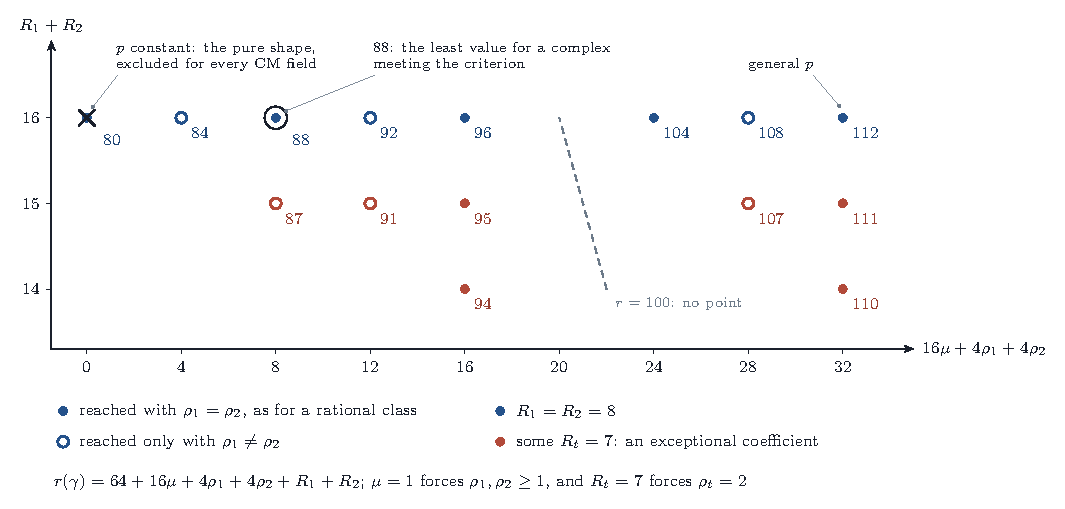
\includegraphics[width=\textwidth]{fig_quarticrank}
\caption{The rank $r(\gamma)$ of \Cref{thm:quarticrank}, over the plane of
the Hankel part $16\mu+4\rho_{1}+4\rho_{2}$ and of $R_{1}+R_{2}$. The fifteen
points are the tuples allowed by the two conditions of the theorem, and each
carries its value. Filled points are reached with $\rho_{1}=\rho_{2}$, as the
character of a complex with rational coefficients is
(\Cref{cor:quarticleast}(ii)); red points need an exceptional coefficient
at one place at least. The value $80$ is the pure shape, excluded for every
CM field by \Cref{thm:cmpurefalse}; so $88$ is the least rank a complex
meeting the criterion can have. The level $r=100$ meets no point.}
\label{fig:quarticrank}
\end{figure}

\begin{corollary}[The least object the criterion asks for]
\label{cor:quarticleast}
Let $E$ be as in \Cref{thm:quarticp2prime}\textup{(v)}.
\begin{enumerate}[label=\textup{(\roman*)},leftmargin=2.6em,itemsep=2pt]
\item $\dim\Ext^{2}(E,E)\ge81$.
\item The coefficients of $P$ satisfy $e_{ji}=\iota(e_{ij})$ for the
  nontrivial automorphism $\iota$ of $F_{0}$, so $\rho_{1}=\rho_{2}$, and
  $r(\ch E)$ is one of $80$, $88$, $94$, $95$, $96$, $104$, $110$, $111$,
  $112$.
\item If $\dim\Ext^{2}(E,E)=r(\ch E)$, then $P$ is not constant and
  $\dim\Ext^{2}(E,E)$ is one of $88$, $94$, $95$, $96$, $104$, $110$, $111$,
  $112$. The value $88$ requires $\mu=0$ and $\rho_{1}=\rho_{2}=1$, and it is
  the rank of $N\omega_{1}+\eta_{s}$ for every $s\in F_{0}^{\times}$.
\end{enumerate}
\end{corollary}

\begin{proof}
(i) By \Cref{thm:quarticp2prime}(v), $\dim\Ext^{2}(E,E)\ge r(\ch E)\ge80$. If
$r(\ch E)=80$, then $P$ is a constant by \Cref{thm:quarticrank}(iii), so
$\ch(E)=c+N\omega_{1}$ and \Cref{thm:cmpurefalse} makes the inequality
strict. (ii) Write $\eta_{t}=\tau_{1}(t)\theta_{1}+\tau_{2}(t)\theta_{2}$
as before \Cref{prop:quarticquat}. A polynomial with rational coefficients in the
$\eta_{t}$ becomes, after exchanging $\theta_{1}$ and $\theta_{2}$, the
polynomial whose coefficients are the images under $\iota$ of the old ones,
so $e_{ji}=\iota(e_{ij})$; the Hankel matrix of $\rho_{2}$ is then the image
under $\iota$ of that of $\rho_{1}$, which has the same rank. The values are
those of \Cref{thm:quarticrank}(iii) with $\rho_{1}=\rho_{2}$, the scaling
of (iv) there changing neither $\mu$ nor the $\rho_{t}$. (iii) If $P$ were
constant, \Cref{thm:cmpurefalse} would give $\dim\Ext^{2}(E,E)>r(\ch E)$.
For $P=\eta_{s}$ the pairs are $(\tau_{t}(s),0)$, so $\rho_{1}=\rho_{2}=1$,
$\mu=0$, and $R_{t}=8$ by \Cref{thm:quarticrank}(ii).
\end{proof}

The Weil tori of \Cref{setup:cmweiltori} exclude more than the pure shape.
A polynomial in $\theta_{1},\theta_{2}$ can stay of Hodge type on all of
$S_{F}$, and then the argument of \Cref{thm:cmpurefalse} applies to it.

\begin{proposition}[The characters that the Weil tori exclude]
\label{prop:quarticweiltori}
Let $E$ be as in \Cref{thm:quarticp2prime}\textup{(v)}, and suppose that $P$
lies in the span of the $\theta_{1}^{i}\theta_{2}^{j}$ with
$i,j\in\{0,4\}$, as for $\ch(E)=c+N\omega_{1}+b\,\theta_{1}^{4}+
\iota(b)\,\theta_{2}^{4}$ with $b\in F_{0}$. Then $\sigma_{E}$ is not
injective and $\dim\Ext^{2}(E,E)>r(\ch E)$. Consequently, if
$\dim\Ext^{2}(E,E)=r(\ch E)=88$, then $P=c+f(\theta_{1})+f^{\iota}(\theta_{2})$
with $c\in\QQ$, where $f(\theta)$ is a nonzero multiple either of $\theta$ or
of $e^{\lambda\theta}-1$ for some $\lambda\ne0$, and $f^{\iota}$ is obtained
by applying $\iota$ to the coefficients of $f$.
\end{proposition}

\begin{proof}
In the basis before \Cref{thm:quarticrank}, $\theta_{1}$ is a sum of four
products of two classes, one from $V_{\sigma}$ and one from $V_{\bbar\sigma}$
for the two embeddings over $\tau_{1}$, in disjoint sets of basis vectors.
So $\theta_{1}^{4}$ is $4!$ times their product, a nonzero element of
$\bigwedge^{4}V_{\sigma}\otimes\bigwedge^{4}V_{\bbar\sigma}$, that is a
nonzero multiple of $\alpha_{\sigma}\alpha_{\bbar\sigma}$, and likewise for
$\theta_{2}^{4}$. Hence $\ch(E)=N\omega_{1}+P$ lies in the span of the
classes $\alpha_{\Sigma}$, which are of type $(p,p)$ on every member of
$S_{F}$ (\Cref{setup:cmweiltori}); being rational, it is a Hodge class on
every member. Its component of degree four is $N\omega_{1}\ne0$, since $P$
has none, and \Cref{thm:cmpurefalse} applies. If $\dim\Ext^{2}(E,E)=
r(\ch E)=88$, then $\mu=0$ and $\rho_{1}=\rho_{2}=1$ by
\Cref{cor:quarticleast}(iii), so $P$ has no mixed monomials, and by the
paragraph after \Cref{thm:quarticrank} its part in $\theta_{1}$ alone is a
multiple of $e^{\lambda\theta_{1}}-1$, of $\theta_{1}$ or of $\theta_{1}^{4}$;
its part in $\theta_{2}$ alone is obtained by $\iota$, by
\Cref{cor:quarticleast}(ii). In the third case $P$ lies in the span of
$1$, $\theta_{1}^{4}$ and $\theta_{2}^{4}$, which the first part excludes.
\end{proof}

The shape $c+b\,\theta_{1}^{4}+\iota(b)\,\theta_{2}^{4}$ has rank $88$, and
with a multiple of $\theta_{1}^{4}\theta_{2}^{4}$ added it has rank $104$,
by \Cref{thm:quarticrank}: $\rho_{1}=\rho_{2}=1$, $\mu$ is $0$ or $1$, and
$R_{1}=R_{2}=8$, since $(e_{10},\dots,e_{40})=(0,0,0,24b)$ with $b\ne0$ does
not meet $V_{+}\cup V_{-}$. \Cref{prop:quarticweiltori} removes
both. What remains at $88$ is a Chern character whose polynomial part is
exponential or linear in each $\theta_{t}$ separately, such as
$c+\eta_{s}+N\omega_{1}$. For these the classes $\theta_{t}$ are not of Hodge
type on the Weil tori, and the argument needs a family of complex tori along
which the character stays of Hodge type and whose members are not algebraic.
The next proposition, the analogue for a quartic field of
\Cref{prop:p2primelocus}(iii) and (iv), shows that there is none: the Hodge
locus of such a character is the polarised family itself.

\begin{proposition}[The Hodge locus of a character at a quartic field]
\label{prop:quarticlocus}
Keep the notation before \Cref{thm:quarticrank}, with $\gamma=\omega+p$ and
every $u_{\sigma}\ne0$, and for the embeddings $\sigma,\bbar\sigma$ over
$\tau_{t}$ put $\omega_{t}=u_{\sigma}\alpha_{\sigma}+u_{\bbar\sigma}
\alpha_{\bbar\sigma}$. Call $\tau_{t}$ a \emph{mid place} of $p$ if $p$ has a
monomial $\theta_{1}^{i}\theta_{2}^{j}$ with nonzero coefficient whose exponent
of $\theta_{t}$ is $1$, $2$ or $3$, and call a mid place \emph{exceptional} if
the only such monomial is $\theta_{t}^{2}$ itself and its coefficient $c_{t}$
in $p$ satisfies $c_{t}^{2}\theta_{t}^{4}=\frac34\,\omega_{t}^{2}$, the ratio
of \Cref{prop:p2primelocus}(iv).
\begin{enumerate}[label=\textup{(\roman*)},leftmargin=2.6em,itemsep=2pt]
\item The annihilator of $\gamma$ in $H^{1}(T_{A})$ is the space of $F$-linear
  $\xi\in\bigoplus_{\sigma}\Hom(V_{\sigma}^{1,0},V_{\sigma}^{0,1})$ with
  $\xi\lrcorner\theta_{t}=0$ at every mid place, plus, at each exceptional
  place, a line spanned by an element of $\Hom(V_{\sigma}^{1,0},
  V_{\bbar\sigma}^{0,1})\oplus\Hom(V_{\bbar\sigma}^{1,0},V_{\sigma}^{0,1})$
  with both components nonzero. Its dimension is $8+4a+b$, where $a$ is the
  number of places that are not mid places and $b$ the number of exceptional
  places.
\item The connected component through $A$ of the Hodge locus of $\gamma$, in
  the space of complex structures on the real torus underlying $A$, is
  $S_{F}$ when neither place is a mid place, that is when $p$ lies in the
  span of the $\theta_{1}^{i}\theta_{2}^{j}$ with $i,j\in\{0,4\}$; and it is
  $\cD_{F}$ when both places are mid places and neither is exceptional. In
  the second case all its members are abelian varieties polarised by
  $\theta_{1}+\theta_{2}$.
\item If both places are exceptional, then near $A$ the Hodge locus is the
  orbit of $A$ under $G_{1}\times G_{2}$, where $G_{t}\cong\mathrm{Spin}(4,3)$
  is the connected stabiliser of $X_{t}=\omega_{t}+c_{t}\theta_{t}^{2}$ in the
  real linear group of $V_{\sigma}\oplus V_{\bbar\sigma}$, and it has
  dimension $10$. A very general member $T$ of it has $\NS(T)=0$ and
  $\Hdg^{2}(T)\otimes\CC$ contained in the span of $X_{1}$ and $X_{2}$, and on
  every member, for every K\"ahler class $\kappa$, $\int X_{t}\,\kappa^{6}$ is
  nonzero with the sign of $c_{t}$, in the normalisation in which
  $\theta_{t}$ is a real class with $\theta_{t}^{2}$ positive.
\item If $\gamma$ is the complexified character of \Cref{thm:quarticp2prime}(v),
  then both places are mid places or neither is, and both are exceptional or
  neither is; and an exceptional $\gamma$ has $r(\gamma)=94$, or $110$ when
  $p$ contains $\theta_{1}^{4}\theta_{2}^{4}$.
\end{enumerate}
\end{proposition}

\begin{proof}
(i) Grade $\bigwedge^{*}H^{1}$ by the degrees in the four $V_{\sigma}$, and
write $\xi_{\sigma\sigma'}$ for the component of $\xi$ in
$\Hom(V_{\sigma'}^{1,0},V_{\sigma}^{0,1})$, which raises the degree in
$V_{\sigma}$ by one and lowers that in $V_{\sigma'}$ by one. The monomial
$\theta_{1}^{i}\theta_{2}^{j}$ has degree $i$ in the two embeddings over
$\tau_{1}$ and $j$ in those over $\tau_{2}$, and $\alpha_{\sigma}$ has degree
$4$ in $V_{\sigma}$. By the proof of \Cref{thm:quarticp2prime}(i),
$\xi_{\sigma\sigma}\lrcorner\omega=0$, and for $\sigma\ne\sigma'$ the only
term of $\xi_{\sigma\sigma'}\lrcorner\omega$ is
$u_{\sigma'}\xi_{\sigma\sigma'}\lrcorner\alpha_{\sigma'}$, of degree $3$ in
$V_{\sigma'}$ and $1$ in $V_{\sigma}$, which determines $\xi_{\sigma\sigma'}$.
A term $\xi_{\rho\rho'}\lrcorner\theta_{1}^{i}\theta_{2}^{j}$ has that degree
only if $\sigma,\sigma'$ lie over the same place $\tau_{t}$, $(i,j)$ is
$(2,0)$ or $(0,2)$ with the $2$ at $t$, and $(\rho,\rho')=(\sigma',\sigma)$.
So every component $\xi_{\sigma\sigma'}$ with $\sigma,\sigma'$ over different
places vanishes, and the equations split into the $F$-linear part and, at
each place, the pair $\xi'=\xi_{\bbar\sigma\sigma}$, $\xi''=\xi_{\sigma\bbar\sigma}$.

For $F$-linear $\xi$ put $D_{t}=\xi\lrcorner\theta_{t}\in V_{\sigma}^{0,1}
\otimes V_{\bbar\sigma}^{0,1}$; the map $\xi\mapsto(D_{1},D_{2})$ is onto, with
kernel $T_{[A]}\cD_{F}$. Then $\xi\lrcorner\theta_{1}^{i}\theta_{2}^{j}
=i\,\theta_{1}^{i-1}\theta_{2}^{j}D_{1}+j\,\theta_{1}^{i}\theta_{2}^{j-1}D_{2}$,
the monomials lie in different degrees, and the two terms have different
Hodge types at the two places, so each vanishes. Now $\theta_{t}^{3}D_{t}=0$
for every $D_{t}$, as a degree count shows, while multiplication by
$\theta_{t}^{k}$ is injective on $V_{\sigma}^{0,1}\otimes V_{\bbar\sigma}^{0,1}$
for $k\le2$: $\theta_{t}^{2}y_{\sigma,k}y_{\bbar\sigma,l}$ is $2$ times the
product of $y_{\sigma,k}y_{\bbar\sigma,l}$ with the two terms of $\theta_{t}$
that avoid $y_{\sigma,k}$ and $y_{\bbar\sigma,l}$, and different $(k,l)$ give
different monomials. Multiplication by $\theta_{t'}^{j}$, $j\le4$, acts on the
other factor of $\bigwedge^{*}H^{1}=\bigwedge^{*}(V_{\sigma}\oplus
V_{\bbar\sigma})\otimes\bigwedge^{*}(V_{\sigma'}\oplus V_{\bbar\sigma'})$ and is
nonzero there. So the conditions on the $F$-linear part are exactly $D_{t}=0$
at the mid places, a space of dimension $16-4(2-a)=8+4a$.

At a place $\tau_{t}$ let $c_{t}$ be the coefficient of $\theta_{t}^{2}$ in $p$.
The terms involving $\xi''$ are $u_{\bbar\sigma}\xi''\lrcorner
\alpha_{\bbar\sigma}+c_{t}\,\xi'\lrcorner\theta_{t}^{2}$, of degree $3$ in
$V_{\bbar\sigma}$ and $1$ in $V_{\sigma}$, the same with $\sigma$ and
$\bbar\sigma$ and with $\xi'$ and $\xi''$ exchanged, and
$i\,\theta_{t}^{i-1}\theta_{t'}^{j}(\xi'\lrcorner\theta_{t})$ and its analogue
for $\xi''$ for every other monomial with exponent $i\in\{1,2,3\}$ of
$\theta_{t}$. Here $\xi'\lrcorner\theta_{t}$ lies in the line
$\bigwedge^{2}V_{\bbar\sigma}^{0,1}$, on which multiplication by
$\theta_{t}^{i-1}\theta_{t'}^{j}$ is injective for $i\le3$ by the same count. If
such another monomial occurs, $\xi'\lrcorner\theta_{t}=\xi''\lrcorner
\theta_{t}=0$, and then $\xi'=\xi''=0$, the maps $\xi'\mapsto
\xi'\lrcorner\alpha_{\sigma}$ and $\xi''\mapsto\xi''\lrcorner\alpha_{\bbar\sigma}$
being injective. Otherwise $\xi''\lrcorner\theta_{t}^{2}=2\theta_{t}\,
(\xi''\lrcorner\theta_{t})$ is a multiple of $\theta_{t}\,y_{\sigma,1}
y_{\sigma,2}$, which is $\xi'_{0}\lrcorner\alpha_{\sigma}$ for one element
$\xi'_{0}$, and likewise with $\sigma$ and $\bbar\sigma$ exchanged; so $\xi'$
and $\xi''$ are multiples of $\xi'_{0}$ and $\xi''_{0}$. Explicitly,
$\xi'_{0}(x_{\sigma,1})=-y_{\bbar\sigma,2}$ and
$\xi'_{0}(x_{\sigma,2})=y_{\bbar\sigma,1}$ give
$\xi'_{0}\lrcorner\alpha_{\sigma}=\theta_{t}\,y_{\sigma,1}y_{\sigma,2}$ and
$\xi'_{0}\lrcorner\theta_{t}=2y_{\bbar\sigma,1}y_{\bbar\sigma,2}$, and
symmetrically for $\xi''_{0}$. Writing $\xi'=a\xi'_{0}$ and
$\xi''=b\xi''_{0}$, the two remaining equations are
$u_{\sigma}a+4c_{t}b=0$ and $4c_{t}a+u_{\bbar\sigma}b=0$, and their
determinant vanishes exactly when $16c_{t}^{2}=u_{\sigma}u_{\bbar\sigma}$. Since $\theta_{t}^{4}=24\,
\alpha_{\sigma}\alpha_{\bbar\sigma}$ and $\omega_{t}^{2}=2u_{\sigma}
u_{\bbar\sigma}\alpha_{\sigma}\alpha_{\bbar\sigma}$, that is the condition
$c_{t}^{2}\theta_{t}^{4}=\frac34\omega_{t}^{2}$, and the solutions then form a
line on which both components are nonzero.

(ii) By \Cref{prop:p2primelocus}(i), applied to each homogeneous component,
the Hodge locus of $\gamma$ in the chart at $A$ is the linear space
$\Ann_{H^{1}(T_{A})}(\gamma)$. If neither place is a mid place, that space is
the space of all $F$-linear $\xi$, which is also the part of $S_{F}$ in the
chart; $\gamma$ is of Hodge type on all of $S_{F}$, as in the proof of
\Cref{prop:quarticweiltori}, and at every member of $S_{F}$ its component of
degree four is $\omega$, whose annihilator in $H^{1}(T)$ is again the space of
$F$-linear deformations (\Cref{thm:quarticp2prime}(i), whose proof uses only
the decomposition into the $V_{\sigma}$). So $S_{F}$ is open in the Hodge locus;
it is closed in the space of complex structures, since commuting with $F$ is a
closed condition and the dimensions of the $H^{1,0}\cap V_{\sigma}$ are
locally constant on it; and it is connected. If both places are mid places
and neither is exceptional, the annihilator is $T_{[A]}\cD_{F}$ by (i), at
every member of $\cD_{F}$, since the conditions of (i) are stated in terms of
the flat classes $\theta_{t}$ and $\omega_{t}$; and the argument of
\Cref{prop:p2primelocus}(iii) shows that $\cD_{F}$ is open, closed and
connected in the Hodge locus.

(iii) At each place $X_{t}$ is, in the $8$-dimensional space
$V_{\sigma}\oplus V_{\bbar\sigma}$ with the form $\theta_{t}$, the class of
\Cref{rem:p2primeexceptional}, and the argument there applies word for
word, with the factor $\mathfrak{su}(2,2)$ at $\tau_{t}$ of the Lie algebra of $G_{F}$
in place of the Hodge group: the stabiliser is $\mathfrak{so}(4,3)$, with an
orbit of dimension $5$ in the Grassmannian. The other components of $\gamma$ are constants, multiples of
$\theta_{t}^{4}$, which is $24$ times the volume form of
$V_{\sigma}\oplus V_{\bbar\sigma}$, and of $\theta_{1}^{4}\theta_{2}^{4}$, all
fixed by $G_{1}\times G_{2}$. So the orbit of $A$ lies in the Hodge locus,
and it has dimension $10$, which by (i) is that of the locus near $A$. A
rational class of Hodge type at a very general member is of Hodge type on the
whole orbit, hence killed by the complex structures of all its members,
which lie in $\mathfrak{g}_{1}\oplus\mathfrak{g}_{2}$ and generate an ideal
projecting nontrivially to both simple factors, that is all of it. The
invariants of $\mathfrak{so}(7,\CC)$ in the exterior algebra of its spin
representation are $1$, $X_{t}$ and the volume form
(\Cref{rem:p2primeexceptional}), so in degree two there are none and in
degree four only $X_{1}$ and $X_{2}$. For the sign, a K\"ahler class is
$\kappa_{h}$ for a positive hermitian form $h$ on the tangent space; only the
terms of $\kappa_{h}^{6}$ that contain the whole volume of the other place pair
with $X_{t}$, and they give $\det(h_{t'})$ times $\kappa_{h'}^{2}$ for the
Schur complement $h'$ of $h_{t'}$ in $h$, a positive hermitian form on the
tangent space at $\tau_{t}$. So $\int X_{t}\kappa_{h}^{6}$ is a positive
multiple of the integral of \Cref{rem:p2primeexceptional} for $h'$, which has
the sign of $c_{t}$; and $G_{1}\times G_{2}$ fixes $X_{t}$ and carries K\"ahler
cones to K\"ahler cones.

(iv) An automorphism of $\bbar\QQ$ inducing $\iota$ on $F_{0}$ fixes the
rational class $\gamma$ and exchanges $\theta_{1}$ with $\theta_{2}$ and
$\omega_{1}$ with $\omega_{2}$, so it carries the conditions at $\tau_{1}$ to
those at $\tau_{2}$. An exceptional $p$ lies in the span of $1$,
$\theta_{t}^{2}$, $\theta_{t}^{4}$ and $\theta_{1}^{4}\theta_{2}^{4}$ with
$c_{t}\ne0$, so $\rho_{1}=\rho_{2}=2$, $\mu=1$ exactly when
$\theta_{1}^{4}\theta_{2}^{4}$ occurs, and $(e_{10},\dots,e_{40})$ lies on
$V_{+}\cup V_{-}$, so $R_{1}=R_{2}=7$ by \Cref{thm:quarticrank}(ii); the
formula of \Cref{thm:quarticrank}(i) gives $94$ or $110$.
\end{proof}

\begin{corollary}[The Weil tori at rank $88$]\label{cor:quarticlocus}
Let $E$ be as in \Cref{thm:quarticp2prime}\textup{(v)} with
$\dim\Ext^{2}(E,E)=r(\ch E)=88$, so that $\ch(E)=N\omega_{1}+c+f(\theta_{1})
+f^{\iota}(\theta_{2})$ as in \Cref{prop:quarticweiltori}. Then the connected
component through $A$ of the Hodge locus of $\ch(E)$ is $\cD_{F}$, and every
complex torus reached from $A$ by a deformation along which $\ch(E)$ stays of
Hodge type is an abelian variety of the family. So no argument that deforms
$E$ itself to a torus that is not algebraic can exclude it; the characters
that such an argument excludes at $88$ are exactly those of
\Cref{prop:quarticweiltori}.
\end{corollary}

\begin{proof}
The coefficient $e_{10}$ of $f$ is nonzero, both for a multiple of $\theta$
and for one of $e^{\lambda\theta}-1$, and $e_{01}=\iota(e_{10})$, so both
places are mid places, with the monomials $\theta_{1}$ and $\theta_{2}$, and
neither is exceptional. \Cref{prop:quarticlocus}(ii) applies.
\end{proof}

As after \Cref{prop:p2primelocus}, this concerns $E$ itself: an
autoequivalence of $D^{b}(A)$ changes the character, and the proposition then
applies to the new one. For the exceptional characters of
\Cref{prop:quarticlocus}(iii), of rank $94$ or $110$, the proof of
\Cref{thm:cmpurefalse} can be started, since the locus contains tori without
divisors, but it breaks down as in \Cref{rem:p2primeexceptional}: the classes
$X_{t}$ have integrals of constant sign against every K\"ahler class, so
Bando and Siu give no vanishing: they bound the signs of the coefficients of
$\ch_{2}$ of a torsion-free sheaf along $X_{1}$ and $X_{2}$, which a complex,
an alternating sum, need not respect. So at a
quartic field the Weil tori and their exceptional analogues exclude exactly
the characters of \Cref{prop:quarticweiltori}, and what the criterion still
asks for, at $88$ and above, is the construction of an object.

The natural candidates are Markman's secant objects \cite{Mar25c}, in the
twisted form in which he states his reduction. For them a $B$-field twist of
$\ch(E)$, the class $\kappa$ of \Cref{thm:quarticobstruction}, is flat, and
under a non-degeneracy condition its component in $H^{4}$ is a polynomial in
the $\eta_{t}$ plus a nonzero Weil class
\cite[Proposition~10.2.1, Theorem~1.1.2]{Mar25c}. But $\ch(E)$ itself is not
flat, and $\kappa$ is not of the form $N\omega+P(\eta)$ in higher degrees
(\Cref{rem:quarticsecantshape}), so they are candidates only for a twisted
form of \Cref{thm:quarticp2prime}(v). The dimension count that works for
imaginary quadratic fields (\Cref{thm:twistedcert}) can be tested on them
exactly. Let $X$ be a principally polarised abelian fourfold with real
multiplication by the ring of integers $\cO_{F_{0}}$, write
$\theta_{1},\theta_{2}\in H^{2}(X,\RR)$ for the components of the
polarisation at the two real places of $F_{0}$, so that
$\theta=\theta_{1}+\theta_{2}$ and $\theta_{j}^{3}=0$, and let $\mathcal{R}$ be
the $\QQ$-subalgebra of $H^{\mathrm{ev}}(X,\QQ)$ spanned by the rational
combinations of the $\theta_{1}^{a}\theta_{2}^{b}$, $0\le a,b\le2$. A class
$v=\sum_{a,b}V_{ab}\,\theta_{1}^{a}\theta_{2}^{b}/(a!\,b!)$ of $\mathcal{R}$ has a
$3\times3$ matrix $V$ with entries in $F_{0}\otimes\RR$.

\begin{proposition}[The secant space of a quartic field]\label{prop:quarticsecant}
Let $F=F_{0}(\sqrt{-q})$ with $q\in F_{0}$ totally positive, let $t\in F_{0}$,
$s_{j}=\sqrt{-1}\,\sqrt{\tau_{j}(q)}$, and for $\varepsilon\in\{\pm1\}^{2}$ put
$e_{\varepsilon}=\exp\bigl(\sum_{j}(\tau_{j}(t)+\varepsilon_{j}s_{j})\theta_{j}\bigr)$.
\begin{enumerate}[label=\textup{(\roman*)},leftmargin=2.6em,itemsep=2pt]
\item The span $S(t,q)$ of the four $e_{\varepsilon}$ is a rational subspace of
  $\mathcal{R}$ of dimension $4=2^{[F_{0}:\QQ]}$, secant to the spinor variety.
  For $t=0$ it is the secant space of \cite[\S11.1, (11.1.2)]{Mar25c} for the
  polarisation $\theta$ and $q$; replacing $\theta$ by $f\theta$,
  $f\in F_{0}^{\times}$, replaces $q$ by $qf^{2}$, and a rational $F_{0}$-$B$-field
  $t$ transports Markman's $F$-structure by the rational automorphism of
  $X\times\widehat X$ acting on $H^{*}(X)$ as $e^{\theta_{t}}$,
  $\theta_{t}=\sum_{j}\tau_{j}(t)\theta_{j}$, and replaces $S(0,q)$ by
  $S(t,q)=e^{\theta_{t}}S(0,q)$.
\item For $v=\sum_{\varepsilon}w_{\varepsilon}e_{\varepsilon}\in S(t,q)$ let
  $\rho=\rk V$ and $N_{w}=\#\{\varepsilon:w_{\varepsilon}\ne0\}$. The ranks of
  contraction from $HT^{k}(X)$ into $v$ are $1$, $8$ and $2\rho+4N_{w}$ for
  $k=0,1,2$, with $(\rho,N_{w})\in\{(1,4),(2,4),(2,2)\}$, and $N_{w}=2$ only for
  biquadratic $F$ and $v$ in the secant plane of one of its two imaginary
  quadratic subfields \cite[\S11.2.1]{Mar25c}.
\item For $v=e^{\theta_{t}}(a\,u+v_{f}+c\,w)$ in the basis
  $u=(1-\tfrac12q_{1}\theta_{1}^{2})(1-\tfrac12q_{2}\theta_{2}^{2})$,
  $v_{f}=\theta_{f}-\tfrac12\theta_{\bar fq}\theta_{1}\theta_{2}$,
  $w=\theta_{1}\theta_{2}$ of $e^{-\theta_{t}}S(t,q)$, one has
  $\chi(v,v)=\int_{X}v^{\vee}v=4\bigl(\Nm(q)a^{2}+c^{2}+\Tr(\bar q f^{2})\bigr)$,
  which is positive definite.
\end{enumerate}
\end{proposition}

\begin{proof}
(i) The Galois group permutes the four exponentials as it permutes the CM
types of $F$, so their span is rational; since $\theta_{j}^{3}=0$,
$e^{\pm s_{j}\theta_{j}}=(1-\tfrac12\tau_{j}(q)\theta_{j}^{2})\pm s_{j}\theta_{j}$, and
the four classes are independent. The conjugates in
$\mathfrak{so}\cap\End^{0}(X\times\widehat X)$ of the standard structure have
eigenvalues $t\pm s$, and the pure spinors of their eigenspaces are the
$e_{\varepsilon}$.

(ii) Over $\CC$, $H^{1}(X)=U_{1}\oplus U_{2}$ with $U_{j}$ the
eigenspaces of $F_{0}$, and $HT^{*}(X)$ and $H^{*}(X)$ are tensor products over
$j$, compatibly with contraction. By \Cref{lem:bfield}(i),
$\xi\lrcorner e^{\lambda\theta_{j}}=y^{\lambda}(\xi)e^{\lambda\theta_{j}}$, and the
blocks $HT_{1}^{a}\otimes HT_{2}^{b}$ have independent images because they
shift the two Hodge bidegrees by $(a,b)$ while $v$ is balanced. The block
$(1,1)$ contributes $4N_{w}$, by the invertibility of the Hadamard matrix of
the signs; the blocks $(2,0)$ and $(0,2)$ contribute $\rho$ each; the blocks
$(1,0)$ and $(0,1)$ contribute $4$ each in degree one. Reality gives
$w_{-\varepsilon}=\overline{w_{\varepsilon}}$, and when $F$ is not biquadratic
the Galois group acts transitively on the CM types, so $N_{w}=4$.

(iii) One has
$\int_{X}e^{c_{1}\theta_{1}+c_{2}\theta_{2}}=c_{1}^{2}c_{2}^{2}$, and $\chi$ is
invariant under $e^{\theta_{t}}$; the form is positive definite because $q$ is
totally positive.
\end{proof}

The integral classes of $\mathcal{R}$ are described by one congruence, and
the description does not depend on the field.

\begin{lemma}[The integral classes of $\mathcal{R}$]\label{lem:quarticlattice}
Let $F_{0}$ be a real quadratic field with ring of integers $\cO$ and
different $\mathfrak d$, and let $X$ be a principally polarised abelian
fourfold with real multiplication by $\cO$. A class $v\in\mathcal{R}$ with
matrix
\[
  V=\begin{pmatrix}r&\bar h&\bar g\\ h&c&\bar k\\ g&k&m\end{pmatrix},
  \qquad r,c,m\in\QQ,\quad h,g,k\in F_{0},
\]
lies in $H^{\mathrm{ev}}(X,\ZZ)$ if and only if $r,c,m\in\ZZ$,
$h,g,k\in\cO$ and $c\equiv g$ modulo $\mathfrak d$.
\end{lemma}

\begin{proof}
Integrality can be tested one prime $p$ at a time, and after a faithfully
flat extension of $\ZZ_{p}$. Let $M=H_{1}(X,\ZZ)$ and let $\langle\,,\rangle$
be the polarisation form on $M$, that is, $\theta$. The Rosati involution fixes
$\cO$, so $\langle\,,\rangle=\Tr_{F_{0}/\QQ}\psi$ for a unique $\cO$-bilinear
alternating form $\psi$ with values in $\mathfrak d^{-1}$, and $\psi$ is
perfect because $\theta$ is principal. Write $\cO=\ZZ[\nu]$ and
$\delta=\nu-\bar\nu$, a generator of $\mathfrak d$
with $\bar\delta=-\delta$, and put $\cO_{p}=\cO\otimes\ZZ_{p}$, a product of
at most two discrete valuation rings. The form $\delta\psi$ on
$M_{p}=M\otimes\ZZ_{p}$ is perfect with values in $\cO_{p}$, so $M_{p}$ has a
symplectic $\cO_{p}$-basis $e,f,e^{*},f^{*}$. Hence
$M_{p}=\cO_{p}\otimes_{\ZZ_{p}}W$, with $W$ the $\ZZ_{p}$-span of this basis,
and $\langle\,,\rangle=B\otimes\omega_{0}$, where $\omega_{0}$ is the standard
symplectic form of $W$ and $B(\alpha,\beta)=\Tr(\delta^{-1}\alpha\beta)$.

Let $\Lambda$ be the ring of integers of a finite extension of $\QQ_{p}$ over
which $F_{0}$ splits, and fix an embedding of $F_{0}$ in its field of
fractions. The map $\alpha\otimes\lambda\mapsto(\alpha\lambda,\bar\alpha\lambda)$
identifies $\cO_{p}\otimes_{\ZZ_{p}}\Lambda$ with the lattice of pairs
$(x,y)\in\Lambda^{2}$ with $x\equiv y$ modulo $\delta$, whose basis is
$(1,1),(\delta,0)$. Let $\varepsilon_{1},\varepsilon_{2}$ be the coordinates
and $u_{1},\dots,u_{4}$ the basis of $W^{\vee}$ dual to $e,f,e^{*},f^{*}$. The
dual lattice has basis $\varepsilon_{2}$, $(\varepsilon_{1}-\varepsilon_{2})/\delta$,
so $H^{1}(X,\Lambda)$ has the basis
\[
  Y_{i}=\varepsilon_{2}\otimes u_{i},\qquad
  Z_{i}=\delta^{-1}(X_{i}-Y_{i}),\qquad\text{where }X_{i}=\varepsilon_{1}\otimes u_{i},
\]
and $H^{*}(X,\Lambda)$ is the exterior algebra on the $Y_{i}$ and $Z_{i}$. In
these coordinates $B=\delta^{-1}(\varepsilon_{1}^{2}-\varepsilon_{2}^{2})$, and the
components of $\theta=B\otimes\omega_{0}$ in the two eigenspaces of $\cO$, the
first being the one on which $\cO$ acts through the fixed embedding, are
\[
  \theta_{1}=\delta^{-1}(X_{1}X_{3}+X_{2}X_{4}),\qquad
  \theta_{2}=-\delta^{-1}(Y_{1}Y_{3}+Y_{2}Y_{4}).
\]
Substitute $X_{i}=Y_{i}+\delta Z_{i}$ in $v=\sum_{a,b}V_{ab}\,\theta_{1}^{a}
\theta_{2}^{b}/(a!\,b!)$ and expand in the monomials in the $Y_{i}$ and $Z_{i}$.
Up to sign, every coefficient is one of
\[
  r,\ m,\ h,\ k,\ c,\ g,\ g-c,\ \delta h,\ \delta k,\ \delta g,\ \delta^{2}g,\
  \frac{g-c}{\delta},\ \frac{h-\bar h}{\delta},\ \frac{k-\bar k}{\delta},\
  \frac{2c-g-\bar g}{\delta^{2}},
\]
and each of $r$, $m$, $h$, $k$, $c$, $g$ and $(g-c)/\delta$ occurs, so an
integral class satisfies the conditions at $p$. Conversely, suppose that they
hold. Every $x\in\cO_{p}$ has $x-\bar x\in\delta\cO_{p}$, which disposes of
$h-\bar h$ and $k-\bar k$; and $g=c+\delta g'$ with $g'\in\cO_{p}$ gives
$2c-g-\bar g=-\delta(g'-\bar g')\in\delta^{2}\Lambda$. So every coefficient
lies in $\Lambda$. When $p$ is unramified in $F_{0}$, $\delta$ is a unit at
$p$ and the congruence is empty.
\end{proof}

\begin{proposition}[Integral secant classes of small Euler characteristic]
\label{prop:quarticother}
Let $F_{0}=\QQ(\sqrt D)$ with $D>1$ squarefree, let $X$ be a principally
polarised abelian fourfold with real multiplication by $\cO_{F_{0}}$, and let
$v$ be an integral class in a space $S(t,q)$ of \Cref{prop:quarticsecant},
with $\rho$ and $N_{w}$ as there.
\begin{enumerate}[label=\textup{(\roman*)},leftmargin=2.6em,itemsep=2pt]
\item If $\rho=1$, then $\chi(v,v)\ne4$.
\item If $\rho=2$ and $N_{w}=4$, then $\chi(v,v)\ne6$.
\end{enumerate}
\end{proposition}

\begin{proof}
By \Cref{lem:quarticlattice} the entries of $V$ lie in $\cO=\cO_{F_{0}}$, the
diagonal ones in $\ZZ$, and $c\equiv g$ modulo $\mathfrak d$; conjugation is
trivial on $\cO/\mathfrak d$.

(i) Write $V=\lambda\alpha\bar\alpha^{T}$ with $\alpha\in\cO^{3}$, and let
$\mathfrak a$ be the ideal generated by the entries of $\alpha$; replacing
$\alpha$ by a multiple, we may take $\mathfrak a$ integral and prime to
$\mathfrak d$. The entries $\lambda\alpha_{i}\bar\alpha_{j}$ lie in $\cO$ and
generate $\lambda\mathfrak a\bar{\mathfrak a}=\lambda\Nm(\mathfrak a)\cO$, so
$\mu=\lambda\Nm(\mathfrak a)\in\ZZ$. With $D'=\alpha_{1}^{2}-\alpha_{0}\alpha_{2}
\in\mathfrak a^{2}$ one has $\chi=4\lambda^{2}\Nm(D')$, and
$\Nm(D')\in\Nm(\mathfrak a)^{2}\ZZ$, so $\chi=4$ forces $\mu=\pm1$ and
$(D')=\mathfrak a^{2}$. Since conjugation is trivial modulo $\mathfrak d$,
$\alpha_{1}\bar\alpha_{1}-\alpha_{2}\bar\alpha_{0}\equiv D'$ modulo
$\mathfrak a\mathfrak d$, and the congruence $c\equiv g$ gives
$\lambda D'\in\mathfrak d\,\bar{\mathfrak a}^{-1}$. The ideal of $\lambda D'$ is
$\mathfrak a\bar{\mathfrak a}^{-1}$, so $\mathfrak a\subseteq\mathfrak d$, which
is impossible for $\mathfrak a$ prime to $\mathfrak d$ and $\mathfrak d\ne(1)$.

(ii) The matrix $\operatorname{adj}V$ is Hermitian of rank one, so
$\operatorname{adj}V=\mu\,\bar l\,l^{T}$ with $l\in\cO^{3}$, $l^{T}V=0$ and
$\mu\in\QQ^{\times}$. Put $\Delta=l_{1}^{2}-4l_{0}l_{2}$ and
$m=\mu^{2}\Nm(\Delta)$. Replacing $l$ by $\lambda l$, $\lambda\in F_{0}^{\times}$,
replaces $\mu$ by $\mu/\Nm(\lambda)$ and $\Delta$ by $\lambda^{2}\Delta$, so $m$
depends only on $V$. As the entries of $\operatorname{adj}V$ are integral,
$\mu$ is integral at every prime at which $l$ is primitive, and $l$ can be
made primitive at the primes above any given $p$, because
$\cO\otimes\ZZ_{(p)}$ is a principal ideal domain; so $m\in\ZZ$. Let $J$ be
the matrix with rows $(0,0,1)$, $(0,-2,0)$, $(1,0,0)$. Since
$\int_{X}\theta_{1}^{2}\theta_{2}^{2}=4$, one has $\chi(v,v)=\operatorname{tr}
(JVJ\bar V)$; and $\operatorname{adj}J$ has rows $(0,0,2)$, $(0,-1,0)$,
$(2,0,0)$, so that $l^{T}(\operatorname{adj}J)\,l=-\Delta$ and
\[
  \sigma_{2}(JVJ\bar V)=\operatorname{tr}\operatorname{adj}(JVJ\bar V)
  =\mu^{2}\,\Delta\bar\Delta=m .
\]
At a real place, $V=PWQ^{T}$ with $W=(w_{\varepsilon})$ and $P$, $Q$ the
$3\times2$ matrices with columns $(1,\pm s_{1},s_{1}^{2})$ and
$(1,\pm s_{2},s_{2}^{2})$, when $t=0$; multiplication by $e^{\theta_{t}}$
replaces $V$ by $UV\bar U^{T}$ with $U$ unipotent and $U^{T}JU=J$, which
conjugates $JVJ\bar V$, so we may take $t=0$. As
$(1,z,z^{2})\,J\,(1,z',z'^{2})^{T}=(z-z')^{2}$ and
$w_{-\varepsilon}=\overline{w_{\varepsilon}}$, the nonzero eigenvalues of
$JVJ\bar V$ are $16\Nm(q)\bigl(|w_{++}|\pm|w_{+-}|\bigr)^{2}$, so
\[
  \chi^{2}-4m=\bigl(64\Nm(q)\,|w_{++}|\,|w_{+-}|\bigr)^{2}\ge0,
\]
with equality exactly when $N_{w}=2$. Modulo $\mathfrak d$ one has
$\bar V\equiv V$, $\operatorname{tr}(JV)=g-2c+\bar g\equiv0$ and
$\sigma_{2}(JV)=\operatorname{tr}\bigl(\operatorname{adj}(V)\operatorname{adj}(J)\bigr)
=\mu\,l^{T}(\operatorname{adj}J)\,\bar l\equiv-\mu\Delta$, with $l$ primitive at
the primes dividing $\mathfrak d$. Hence
\[
  \chi\equiv\operatorname{tr}\bigl((JV)^{2}\bigr)
  =\operatorname{tr}(JV)^{2}-2\sigma_{2}(JV)\equiv2\mu\Delta
  \pmod{\mathfrak d}.
\]

Now let $\chi=6$ and $N_{w}=4$. Then $1\le m\le8$, because $\Delta$ is
totally negative, and $m$ satisfies three conditions.
\begin{enumerate}[label=\textup{(\alph*)},leftmargin=2.6em,itemsep=2pt]
\item $4m\equiv36$ modulo $\mathfrak d\cap\ZZ$, which is $D\ZZ$ if
  $D\equiv1$ modulo $4$ and $2D\ZZ$ otherwise. As $D$ is squarefree, this
  says that $m\equiv9$ modulo the odd part $D_{o}$ of $D$.
\item $m\equiv0$ or $1$ modulo $4$. Take $l$ primitive at $2$, so that
  $\mu\in\ZZ_{(2)}$. Since $\Nm(x+4y)\equiv\Nm(x)$ modulo $4$ for
  $x,y\in\cO\otimes\ZZ_{(2)}$, $\Nm(\Delta)\equiv\Nm(l_{1}^{2})=\Nm(l_{1})^{2}$,
  and $m\equiv\bigl(\mu\Nm(l_{1})\bigr)^{2}$ modulo $4$.
\item If $D\equiv2$ modulo $4$, then $m$ is odd. The prime $\mathfrak p$ above
  $2$ is ramified, $v_{\mathfrak p}(2)=2$ and $v_{\mathfrak p}(\sqrt D)=1$, so
  $v_{\mathfrak p}(\mathfrak d)=3$ while $v_{\mathfrak p}(6)=2$; the congruence
  $6\equiv2\mu\Delta$ modulo $\mathfrak p^{3}$ forces
  $v_{\mathfrak p}(\mu\Delta)=0$, so $\mu$ and $\Nm(\Delta)$ are odd.
\end{enumerate}
If $D\equiv1$ modulo $4$ and $D\ne5$, then $D\ge13$ and (a) has no solution
in $[1,8]$. If $D\equiv3$ modulo $4$, (a) gives $m\in\{3,6\}$ for $D=3$,
$m=2$ for $D=7$ and nothing for $D\ge11$, and (b) excludes these values. If
$D=2D'$, then (b) and (c) give $m\equiv1$ modulo $4$, which with (a) says
$m\equiv9$ modulo $4D'$, and this has no solution in $[1,8]$ unless $D'=1$.
There remain $D=5$, with $m=4$, and $D=2$, with $m\in\{1,5\}$.

For $\QQ(\sqrt5)$, $m=4$ means that $\Delta$ is $-2$ times a unit or minus the
square of a unit, since $2$ is inert; and $\Delta\equiv l_{1}^{2}$ modulo $4$,
while neither $-1$ nor twice a unit is a square modulo $4$ in $\ZZ[\varphi]$.
For $\QQ(\sqrt2)$, (c) makes $\mu$ odd, so $\mu=\pm1$ and
$\Nm(\Delta)\in\{1,5\}$; the norms of the elements of $\ZZ[\sqrt2]$ prime to
$2$ are $\pm1$ modulo $8$, so $\Nm(\Delta)=1$ and $\Delta=-(1+\sqrt2)^{2k}$,
which is $3$ or $1+2\sqrt2$ modulo $4$, and neither is a square modulo $4$ in
$\ZZ[\sqrt2]$.
\end{proof}

\begin{theorem}[No dimension-count certificate for quartic CM fields]
\label{thm:quarticobstruction}
Let $F=F_{0}(\sqrt{-q})$ be a quartic CM field with real quadratic subfield
$F_{0}$, let $X$ be a principally polarised abelian fourfold with real
multiplication by $\cO_{F_{0}}$, and give $A=X\times\widehat X$ the action of
$F$ of \cite[\S11.1]{Mar25c}, transported by the $B$-field $e^{\theta_{t}}$ for a
rational $t\in F_{0}$. Let $F_{1},F_{2}$
be perfect complexes on $X$ with $\Ext^{<0}(F_{i},F_{i})=0$, for instance
sheaves, whose Chern characters lie in spaces $S(t',q')$ of
\Cref{prop:quarticsecant}, and let $E=\Phi(F_{1}\boxtimes F_{2}^{\vee})$ and
$\kappa=\ch(E)e^{\ell/2}$. Put $v_{1}=\ch(F_{1})$ and $v_{2}=\ch(F_{2}^{\vee})$.
\begin{enumerate}[label=\textup{(\roman*)},leftmargin=2.6em,itemsep=2pt]
\item $r(\kappa)=r(\ch E)=r^{2}(v_{1})+64+r^{2}(v_{2})$, where
  $r^{2}(v_{i})\in\{12,18,20\}$ is given by \Cref{prop:quarticsecant}(ii); so
  $r(\kappa)\le104$, and $r(\kappa)\in\{100,102,104\}$ unless $F$ is
  biquadratic and some $v_{i}$ has $N_{w}=2$.
\item $\dim\Ext^{2}(E,E)>r(\kappa)$. So the injectivity of $\sigma_{E}$ cannot
  be obtained from a dimension count for any such $E$.
\item If $t=0$ and both Chern characters lie in $S(0,q)$, then $\kappa$ is
  invariant under $G_{F}$, and so is a Hodge class on every member of the
  $(F,2,1)$-family. This is the case $[F:\QQ]=4$ of
  \cite[Proposition~10.2.1(1)]{Mar25c} and of the inclusion stated before
  \cite[Lemma~10.1.3]{Mar25c}, with other conventions for $\Phi$ and for the
  sign of the twist.
\end{enumerate}
\end{theorem}

\begin{proof}
(i) By \Cref{lem:bfield}(i), multiplication by $e^{\ell/2}$ conjugates
contraction by an automorphism of $HT^{2}$, so $r(\kappa)=r(\ch E)$; and, as
in the proof of \Cref{thm:factor}(iv), $\Phi$ identifies $r(\ch E)$ with the
rank of contraction from $HT^{2}(X\times X)=\bigoplus_{a+b=2}HT^{a}(X)\otimes
HT^{b}(X)$ into $v_{1}\boxtimes v_{2}$. Write $r^{k}$ for the rank of
contraction from $HT^{k}(X)$. The block $HT^{1}\otimes HT^{1}$ maps into
$H^{\mathrm{odd}}\otimes H^{\mathrm{odd}}$ by the tensor product of the two
contractions from $HT^{1}$, of rank $r^{1}(v_{1})r^{1}(v_{2})=64$, and the other
two blocks map into $H^{\mathrm{ev}}\otimes H^{\mathrm{ev}}$. If
$(x_{1}\lrcorner v_{1})\otimes v_{2}+v_{1}\otimes(x_{2}\lrcorner v_{2})=0$, then
$x_{1}\lrcorner v_{1}=\lambda v_{1}$ for a scalar $\lambda$, and $\lambda=0$
because contraction from $HT^{2}$ raises $q-p$ by two on classes of type
$(p,q)$ while $v_{1}\ne0$ is of type $(p,p)$; so those two blocks contribute
$r^{2}(v_{1})+r^{2}(v_{2})$, and $r^{2}(v_{i})=2\rho+4N_{w}\in\{12,18,20\}$ by
\Cref{prop:quarticsecant}(ii), with $12$ only for biquadratic $F$.

(ii) By the K\"unneth formula, as in \Cref{prop:orlovfour},
$\dim\Ext^{2}(E,E)=e_{0}e_{2}'+e_{1}e_{1}'+e_{2}e_{0}'$ with
$e_{k}=\dim\Ext^{k}(F_{1},F_{1})\ge r^{k}(v_{1})$, by the commutative square
$\sigma_{F}\circ\operatorname{ev}_{F}=(\,\cdot\,)\lrcorner\ch(F)$, and likewise
for $F_{2}$. So $\dim\Ext^{2}(E,E)\ge r(\kappa)$, with equality only if each
$F_{i}$ is minimal, $\dim\Ext^{k}(F_{i},F_{i})=1,8,r^{2}(\ch F_{i})$ for
$k=0,1,2$. For such $F_{i}$, Serre duality gives $\chi(F_{i},F_{i})=r^{2}-14$,
that is $4$, $6$ or $-2$ for $(\rho,N_{w})=(1,4)$, $(2,4)$, $(2,2)$. The last
is impossible because $\chi$ is positive on $S(t',q')$. The Chern character
of a perfect complex on a complex torus is integral, since by the K\"unneth
theorem the topological $K$-theory of a real torus is generated by products of
classes pulled back from its circle factors, whose Chern characters are
integral. So the first two values are excluded by \Cref{prop:quarticother}.

(iii) Over $\RR$, $H^{1}(X,\RR)=U_{1}\oplus U_{2}$, with $U_{j}$ the eigenspace
of $F_{0}$ for $\tau_{j}$, and the $U_{j}$ are orthogonal for $\theta$. As in
the proof of \Cref{prop:flatall}, the correspondence $Z\mapsto\ch(\Phi(Z))
e^{\ell/2}$, the Poincar\'e class $\ell=\ell_{1}+\ell_{2}$, the classes $\eta$
and $\gamma$ and the exponentials $e_{\varepsilon}$ all decompose as tensor
products over $j$ of classes of even degree, so that the image of
$e_{\varepsilon}\boxtimes e_{\varepsilon'}^{\vee}$ is the tensor product over $j$
of the images of $e^{\varepsilon_{j}s_{j}\theta_{j}}\boxtimes
e^{-\varepsilon_{j}'s_{j}\theta_{j}}$ in the $j$-th factor. On that factor
$\sqrt{-q}$ acts as in the imaginary quadratic construction with $d$ replaced
by $\tau_{j}(q)$, and the identities of \Cref{prop:flatall} at $n=2$, which
are identities in the exterior algebra of a symplectic space with $d$ a
symbol, show that each image is a multiple of $e^{\pm(s_{j}/2\tau_{j}(q))\eta_{j}}$
or of a Weil class $(\gamma_{j}\mp s_{j}\ell_{j})^{2}$ of the $j$-th factor.
These are invariant under the special unitary group $SU_{j}$ of the $j$-th
factor, and $G_{F}(\RR)=SU_{1}\times SU_{2}$ acts factor by factor; so the
rational class $\kappa$ is invariant under $G_{F}(\RR)$, which is Zariski dense
in $G_{F}$, and the Hodge group of every member of the family lies in $G_{F}$.
\end{proof}

\begin{remark}[The shape of the secant characters]\label{rem:quarticsecantshape}
Let $t=0$ in \Cref{thm:quarticobstruction}(iii), and write
$\eta=\eta_{1}+\eta_{2}$, $\gamma=\gamma_{1}+\gamma_{2}$ and
$\ell=\ell_{1}+\ell_{2}$ for the decompositions over the real places used in
its proof: $\eta_{j}=\tau_{j}(q)\theta_{j}+\widehat\theta_{j}$ and
$\gamma_{j}=\tau_{j}(q)\theta_{j}-\widehat\theta_{j}$, with $\theta_{j}$ and
$\widehat\theta_{j}$ here the pull-backs to $A$ of the components of the
polarisations of $X$ and $\widehat X$. The classes $\eta_{t}$ of $A$ are the
combinations of $\eta_{1}$ and $\eta_{2}$, and the Weil classes at the two
embeddings over $\tau_{j}$ are the multiples of
$(\gamma_{j}\mp s_{j}\ell_{j})^{2}$. Let $\kappa_{(a,b)}$ be the component of
$\kappa$ of degree $a$ at $\tau_{1}$ and $b$ at $\tau_{2}$. Although $\kappa$
is flat, it does not lie in $\CC[\eta_{1},\eta_{2}]+W_{F}\otimes\CC$ once
$\kappa_{4}$ has a nonzero Weil part, unlike the classes of
\Cref{prop:flatall}. Indeed, by the proof of \Cref{thm:quarticobstruction}(iii),
$\kappa$ is a sum of products $X_{1}X_{2}$ in which each $X_{j}$ is a multiple
of $e^{\pm c_{j}\eta_{j}}$, $c_{j}=s_{j}/(2\tau_{j}(q))$, or of
$(\gamma_{j}\mp s_{j}\ell_{j})^{2}$. The components $\kappa_{(4,0)}$ and
$\kappa_{(4,8)}$ receive exactly the terms whose second factor is an
exponential, through its parts of degree $0$ and $8$, and
$c_{2}^{4}=1/(16\tau_{2}(q)^{2})$ for both signs; so
\[
  \kappa_{(4,8)}=\frac{\kappa_{(4,0)}\,\eta_{2}^{4}}{384\,\tau_{2}(q)^{2}},
\]
and symmetrically. The polynomials in $\eta_{1},\eta_{2}$ of this bidegree
are the multiples of $\eta_{1}^{2}\eta_{2}^{4}$ and $W_{F}$ has no component
there, while $\kappa_{(4,0)}$ has a nonzero Weil part as soon as $\kappa_{4}$
has one, since a nonzero rational Weil class has nonzero components at all
four embeddings. The class $\ch(E)=\kappa e^{-\ell/2}$ itself is not flat
when $\rk(E)\ne0$: for $Y$ in the Lie algebra of $G_{F}$,
$D_{Y}\ch(E)=-\tfrac12(D_{Y}\ell)\ch(E)$, whose part of degree two is
$-\tfrac12\rk(E)\,D_{Y}\ell$, and $\ell$ is not flat. So these objects, when
their rank is not zero, are candidates only for a twisted form of \Cref{thm:quarticp2prime}(v), with
hypothesis a flat twisted character $\kappa$ with $\kappa_{4}=N\omega+P_{4}$,
which needs the extension of \Cref{thm:BF} to twisted objects \cite{Per26}
and the extraction of untwisted cycles of \cite[Section~2]{Mar25b}, as after
\Cref{thm:twistedcert}. This is the form in which Markman states his
reduction: he uses the normalised class $\ch(E)\exp(-c_{1}(E)/\rk E)$, which is
$\kappa e^{-\kappa_{1}/\kappa_{0}}$ when $\rk E\ne0$, asserts the shape of a
polynomial plus a nonzero Weil class only for its component in $H^{4}$, and
takes as propagation hypothesis that this component stays algebraic
\cite[Proposition~10.2.1, Corollary~10.2.3]{Mar25c}.
\end{remark}

\begin{remark}[Negative Ext groups]\label{rem:quarticnegext}
The hypothesis $\Ext^{<0}(F_{i},F_{i})=0$ in
\Cref{thm:quarticobstruction}(ii) can be replaced by a condition on the
amplitude. Let $F_{1},F_{2}$ be any perfect complexes with characters in
spaces $S(t',q')$, let $e_{k}=\dim\Ext^{k}(F_{1},F_{1})$ and
$e_{k}'=\dim\Ext^{k}(F_{2},F_{2})$, and put
$\nu_{i}=\sum_{j\ge3}(-1)^{j}\dim\Ext^{-j}(F_{i},F_{i})$. Then still
$\dim\Ext^{2}(E,E)\ge r(\kappa)$, and equality forces, for each $i$,
$\dim\Ext^{k}(F_{i},F_{i})=1,8,r^{2}(v_{i})$ for $k=0,1,2$,
$\Ext^{-1}(F_{i},F_{i})=\Ext^{-2}(F_{i},F_{i})=0$ and
$\nu_{i}=\bigl(\chi(v_{i},v_{i})-r^{2}(v_{i})+14\bigr)/2$. This gives
$\nu_{i}\ge2$ for $(\rho,N_{w})=(1,4)$ and $(2,2)$, and $\nu_{i}\ge1$ for
$(2,4)$ unless $F_{0}=\QQ(\sqrt3)$ and $\chi(v_{i},v_{i})=4$, where
$\nu_{i}=-1$, a case that needs integral classes of that kind. So
equality needs, for both $i$, some $\Ext^{-j}(F_{i},F_{i})\ne0$ with $j\ge4$
even, or $j\ge3$ odd in the exceptional case, and it fails as soon as one
$F_{i}$ has its cohomology sheaves in an interval of length at most $3$, at
most $2$ in the exceptional case. These conditions are necessary, not
sufficient. The strict inequality $\dim\Ext^{2}(E',E')>r(\ch E')$ passes to
the images $E'$ of such an $E$ under derived equivalences, push-forward and
pull-back along isogenies, and twists by line bundles or $B$-fields.

Indeed, $\dim\Ext^{2}(E,E)=\sum_{a\in\ZZ}e_{a}e_{2-a}'$ by the K\"unneth
formula, and $e_{a}=e_{4-a}$ by Serre duality. The terms $a=0,1,2$ give at
least $r(\kappa)$, with equality only if $e_{k}$ and $e_{k}'$ are the ranks
$r^{k}$ for $k\le2$, as in the proof of \Cref{thm:quarticobstruction}(ii); the
terms $a=3,4,-1,-2$ are $e_{1}e_{-1}'$, $e_{0}e_{-2}'$, $e_{-1}e_{1}'$ and
$e_{-2}e_{0}'$, which must vanish. Then
$\chi(F_{i},F_{i})=2e_{0}-2e_{1}+e_{2}+2\sum_{j\ge1}(-1)^{j}e_{-j}$ gives the
value of $\nu_{i}$. The number $\chi(v,v)$ is a positive even integer:
positive by \Cref{prop:quarticsecant}(iii), and even because $\int_{X}x^{2}$ is
even for $x\in H^{4}(X,\ZZ)=\bigwedge^{4}H^{1}(X,\ZZ)$. For $(1,4)$,
$\chi\in4\ZZ$ by the proof of \Cref{prop:quarticother}(i), and $\chi\ne4$; for
$(2,2)$, $r^{2}=12$. For $(2,4)$, $r^{2}=20$, and in the proof of
\Cref{prop:quarticother}(ii) $\chi^{2}-4m>0$ with $m\ge1$, so $\chi\ge4$, and
$\chi\ne6$. If $\chi=4$, then $m\in\{1,2,3\}$, and conditions (a) to (c) of
that proof, with $36$ replaced by $16$, say that $m\equiv4$ modulo the odd
part of $D$, so that $D\in\{2,3,6\}$; that $m=1$; and, for $D\equiv2$ modulo
$4$, that $m$ is even, because $v_{\mathfrak p}(4)=4\ge3$ here gives
$v_{\mathfrak p}(\mu\Delta)\ge1$. Only $D=3$ remains. A complex with cohomology
sheaves in an interval of length $l$ has $\Ext^{-j}(F,F)=0$ for $j>l$.
Equivalences preserve Ext algebras and, through the induced isomorphisms of
$HT^{*}$ and $H^{*}$, ranks of contraction (\cite{CRV12}, as in the proof of
\Cref{thm:factor}(iv)); for an isogeny $g$,
$g^{*}g_{*}E=\bigoplus_{x\in\ker g}t_{x}^{*}E$, so $\Ext^{2}(g_{*}E,g_{*}E)$
contains $\Ext^{2}(E,E)$ while $r(\ch g_{*}E)=r(\ch E)$, and likewise for
$g^{*}$; twists are \Cref{lem:bfield}(i).
\end{remark}

What \Cref{thm:quarticobstruction} and \Cref{rem:quarticnegext} leave for
$\mathbf{W}(F,2,\delta)$ is one of three things: an Orlov product both of
whose factors have nonzero Ext groups in some even degree at most $-4$ (or odd
degree at most $-3$ when $F_{0}=\QQ(\sqrt3)$); a kernel on $X\times X$ that is
not an external product; or a proof of the injectivity of $\sigma_{E}$ for
some Orlov product that does not go through a dimension count, which is what
Markman's question \cite[Question~11.2.2]{Mar25c} asks for. The next
proposition shows that a kernel whose transform has a pure spinor as its
character, for instance a line bundle on the graph of a homomorphism, gives no
Weil class.

\begin{proposition}[Pure spinors give no Weil class]
\label{prop:quarticexclusions}
Keep the notation of \Cref{rem:quarticsecantshape} on $A=X\times\widehat X$
with $t=0$, let $V_{j}\subseteq H^{1}(A,\RR)$ be the part at $\tau_{j}$, and
call a class flat if it is invariant under $G_{F}(\RR)$. Let
$v=c\,e^{\beta}\Omega_{N}$ be a real pure spinor, with $c\in\RR^{\times}$,
$\beta$ a real $2$-form, $N\subseteq H^{1}(A,\RR)$ and $\Omega_{N}$ a
generator of $\det N$. If $v$ is flat, then $N$ is one of $0$, $V_{1}$,
$V_{2}$, $H^{1}(A,\RR)$, and $v\in\RR[\eta_{1},\eta_{2}]$. This applies to
the characters of line bundles on translates of abelian subvarieties, of
points and of simple semi-homogeneous bundles, and of their images under
derived equivalences and isogenies, twisted by any real $B$-field; for
instance to $\Phi$ of a line bundle on the graph of a homomorphism $X\to
X\times X$. The component in $W_{F}\otimes\RR$ of such a class vanishes in
every degree: no such object has a character, twisted as stated, of the form
required by \Cref{thm:quarticp2prime}(v) or by its twisted form, whatever
the quartic field.
\end{proposition}

\begin{proof}
Over $\RR$, $G_{F}(\RR)=SU_{1}\times SU_{2}$ with $SU_{j}$ acting on $V_{j}$
and trivially on the other part, and $V_{j}\otimes\CC$ is the sum of the
standard representation of $SU_{j}\otimes\CC\cong\SL_{4}$ and its dual, which
are not isomorphic (proof of \Cref{prop:quarticquat}(i)). So $V_{1}$ and
$V_{2}$ are irreducible and not isomorphic, and $0$, $V_{1}$, $V_{2}$,
$H^{1}(A,\RR)$ are the only stable subspaces. The flat classes are
$\mathrm{Inv}_{1}\otimes\mathrm{Inv}_{2}$, where by the same proof
$\mathrm{Inv}_{j}\subseteq\bigwedge^{*}V_{j}$ is spanned by the powers of
$\eta_{j}$ and the two Weil classes $(\gamma_{j}\mp s_{j}\ell_{j})^{2}$; in
degree two it is $\RR\eta_{j}$, and $\eta_{j}^{4}$ spans $\bigwedge^{8}V_{j}$.

If $v$ is real and pure over $\CC$, then $N=\{\xi:\xi\wedge v=0\}$ is
defined over $\RR$, and so are $c$ and the class of $\beta$ modulo
$N\wedge H^{1}$. For $g\in G_{F}(\RR)$, $gv=v$ gives $gN=N$, and
$g\Omega_{N}=\det(g|_{N})\Omega_{N}=\Omega_{N}$ because the connected
semisimple group $G_{F}(\RR)$ has no nontrivial character. Hence
$(e^{g\beta-\beta}-1)\Omega_{N}=0$, whose part of lowest degree gives
$g\beta-\beta\in N\wedge H^{1}$. So $N$ is one of the four stable subspaces,
and the class of $\beta$ in $\bigwedge^{2}(H^{1}/N)$ is invariant; by complete
reducibility it is the image of an invariant $2$-form
$a_{1}\eta_{1}+a_{2}\eta_{2}$, and since $e^{n\wedge x}\Omega_{N}=\Omega_{N}$
for $n\in N$, $v=c\,e^{a_{1}\eta_{1}+a_{2}\eta_{2}}\Omega_{N}$, with
$\Omega_{N}$ a multiple of $1$, $\eta_{1}^{4}$, $\eta_{2}^{4}$ or
$\eta_{1}^{4}\eta_{2}^{4}$. The characters listed are pure spinors, and
derived equivalences, isogenies and twists preserve purity; this is the
classical description recalled in \Cref{setup:lagquadric} and after
\Cref{cor:naturalsums}.
\end{proof}

\subsubsection*{Markman's candidate for a quartic field}

Markman gives one explicit pair of sheaves for a biquadratic field
\cite[Example~11.2.7, Lemma~11.2.8]{Mar25c} and asks whether the second can
be chosen so that its semiregularity map is injective on the image of the
evaluation map \cite[Question~11.2.2]{Mar25c}. For one object on the fourfold
this is the weakened criterion of \Cref{setup:criterion}, and the local
method of \Cref{thm:candidatefails} decides it for his pair: both sheaves
fail it, at points of the curves that the construction glues in. Two local
computations are needed, one for a sheaf that is locally free on a smooth
support and one for the ideal of a curve in a smooth divisor. As in
\Cref{lem:localproducts}, for a germ of vector field $\theta$ and a perfect
complex $F$ of modules over a local ring we write
$a_{\theta}\in\Ext^{1}(F,F)$ for the class of the jet extension along
$\theta$.

\begin{lemma}[Free germs on smooth supports]\label{lem:freegerm}
Let $\cO$ be the local ring of a smooth complex variety $Y$ at a point $p$,
or its completion, let $C\ni p$ be a smooth subvariety of codimension
$c\ge1$, put $N=T_{p}Y/T_{p}C$, and let $F$ be a perfect complex of
$\cO$-modules quasi-isomorphic to a shift of $\cO_{C,p}^{\oplus r}$, $r\ge1$.
Then $\Ext^{2}_{\cO}(F,F)$ is a free $\cO_{C,p}$-module isomorphic to
$M_{r}(\cO_{C,p})\otimes\bigwedge^{2}N$, and modulo the maximal ideal of
$\cO_{C,p}$ the product $a_{\theta}a_{\theta'}$ is, up to a sign that does
not depend on $\theta,\theta'$, the element $\id\otimes(\bar\theta\wedge\bar\theta')$,
where $\bar\theta,\bar\theta'$ are the images of $\theta(p),\theta'(p)$ in
$N$. In particular $a_{\theta}a_{\theta'}\ne0$ whenever $\theta(p)$,
$\theta'(p)$ and $T_{p}C$ span a space of dimension $\dim C+2$.
\end{lemma}

\begin{proof}
Choose formal coordinates $x_{1},\dots,x_{m}$ at $p$ with
$C=\{x_{1}=\dots=x_{c}=0\}$. Ext groups of finitely generated modules and jet
extensions commute with the flat base change from
$R=\CC[x_{1},\dots,x_{m}]$ to $\cO$, and a shift changes neither the Ext
algebra nor the jet classes, so we may take $F=(R/(x_{1},\dots,x_{c}))^{\oplus r}$
over $R$. Write $R=A_{1}\otimes\dots\otimes A_{c}\otimes B$ with
$A_{i}=\CC[x_{i}]$ and $B=\CC[x_{c+1},\dots,x_{m}]$; then
$F=k_{1}\otimes\dots\otimes k_{c}\otimes B^{\oplus r}$, with $k_{i}$ the
residue field of $A_{i}$ at the origin. On the resolution
$A_{i}\xrightarrow{x_{i}}A_{i}$ of $k_{i}$ the jet chain map of
$\partial_{i}$ is $-\partial_{i}(x_{i})=-1$, as in the proof of
\Cref{lem:localproducts}, so its class $\gamma_{i}$ spans
$\Ext^{1}_{A_{i}}(k_{i},k_{i})=k_{i}$, and $\Ext^{j}_{A_{i}}(k_{i},k_{i})=0$ for
$j\ge2$. The module $B^{\oplus r}$ is free, so its Ext algebra is
$M_{r}(B)$ in degree zero and its jet classes vanish. By
\eqref{eq:kunnethext}, applied factor by factor, $\Ext^{*}_{R}(F,F)$ is the
graded tensor product of the exterior algebra on $\gamma_{1},\dots,\gamma_{c}$
with $M_{r}(B)$, and $a_{\partial_{i}}=\gamma_{i}\otimes\id$ for $i\le c$,
while $a_{\partial_{i}}=0$ for $i>c$. Hence
$\Ext^{2}_{R}(F,F)=\bigwedge^{2}\langle\gamma_{1},\dots,\gamma_{c}\rangle\otimes M_{r}(B)$,
and $B=\cO_{C}$ in these coordinates. For $\theta=\sum_{i}f^{i}\partial_{i}$
and $\theta'=\sum_{i}f'^{i}\partial_{i}$ the linearity of \Cref{lem:edge}
gives
\[
  a_{\theta}a_{\theta'}=\sum_{i,j\le c}f^{i}f'^{j}\,\gamma_{i}\gamma_{j}\otimes\id
  =\sum_{i<j\le c}\bigl(f^{i}f'^{j}-f^{j}f'^{i}\bigr)\,\gamma_{i}\gamma_{j}\otimes\id,
\]
because the $\gamma_{i}$ anticommute and square to zero. The functions
$x_{1},\dots,x_{c}$ act by zero, so modulo the maximal ideal of $\cO_{C}$ the
coefficients are those of $\theta(p)\wedge\theta'(p)$ on
$\partial_{i}\wedge\partial_{j}$, $i<j\le c$, which are the coordinates of
$\bar\theta\wedge\bar\theta'$ in $\bigwedge^{2}N$. A section of a free module
with nonzero reduction is nonzero.
\end{proof}

\begin{lemma}[A curve in a divisor]\label{lem:divisorgerm}
Let $\cO$, $Y$ and $p$ be as in \Cref{lem:freegerm}, let $D\ni p$ be a
smooth divisor, let $C\subset D$ be a smooth subvariety of codimension two in
$D$ through $p$, and let $F$ be quasi-isomorphic to a shift of the ideal
$I_{C\subset D}$ of $C$ in $\cO_{D}$, regarded as an $\cO$-module. Put
$\nu=T_{p}Y/T_{p}D$ and $N'=T_{p}D/T_{p}C$. Then
$\Ext^{2}_{\cO}(F,F)\cong\cO_{C,p}\otimes\nu\otimes N'$, and modulo the maximal
ideal of $\cO_{C,p}$ the product $a_{\theta}a_{\theta'}$ is, up to a fixed
sign, the image of $\theta(p)\wedge\theta'(p)$ under
\[
  \textstyle\bigwedge^{2}T_{p}Y\longrightarrow\bigwedge^{2}(T_{p}Y/T_{p}C)
  \longrightarrow\bigwedge^{2}(T_{p}Y/T_{p}C)\big/\bigwedge^{2}N'\cong\nu\otimes N'.
\]
In particular $a_{\theta}a_{\theta'}\ne0$ whenever $\theta(p)\wedge\theta'(p)$
does not lie in $\bigwedge^{2}T_{p}D+T_{p}C\wedge T_{p}Y$.
\end{lemma}

\begin{proof}
With formal coordinates in which $D=\{x_{1}=0\}$ and $C=\{x_{1}=x_{2}=x_{3}=0\}$,
and the same reduction to the polynomial ring, write
$R=\CC[x_{1}]\otimes\CC[x_{2},x_{3}]\otimes B$ with $B=\CC[x_{4},\dots,x_{m}]$.
Then $I_{C\subset D}=k\otimes\mathfrak m\otimes B$, where $k$ is the residue
field of $\CC[x_{1}]$ and $\mathfrak m=(x_{2},x_{3})$. As in the proof of
\Cref{lem:localproducts}, $\mathfrak m$ has projective dimension one,
$\Ext^{1}(\mathfrak m,\mathfrak m)=\mathfrak m/\mathfrak m^{2}$ has the basis
$\alpha_{2}=a_{\partial_{2}}$, $\alpha_{3}=a_{\partial_{3}}$ and is killed by
$\mathfrak m$, and $\Ext^{2}(\mathfrak m,\mathfrak m)=0$; the factor $k$
contributes $\gamma_{1}$ in degree one, as in \Cref{lem:freegerm}, and $B$
contributes nothing in positive degree. By \eqref{eq:kunnethext}
\[
  \Ext^{2}_{R}(I_{C\subset D},I_{C\subset D})
  =\Ext^{1}(k,k)\otimes\Ext^{1}(\mathfrak m,\mathfrak m)\otimes B
  =\langle\gamma_{1}\rangle\otimes\langle\alpha_{2},\alpha_{3}\rangle\otimes B,
\]
the other summands vanishing by the projective dimensions, and
$a_{\partial_{1}}a_{\partial_{j}}=-a_{\partial_{j}}a_{\partial_{1}}=\pm\gamma_{1}\otimes\alpha_{j}$
for $j=2,3$, while $a_{\partial_{2}}a_{\partial_{3}}=1\otimes\alpha_{2}\alpha_{3}=0$,
$a_{\partial_{1}}^{2}=0$ and $a_{\partial_{i}}=0$ for $i\ge4$. As before,
$a_{\theta}a_{\theta'}$ reduces to the component of $\theta(p)\wedge\theta'(p)$
on $\partial_{1}\wedge\langle\partial_{2},\partial_{3}\rangle$. In these
coordinates $\partial_{1}$ spans $\nu$, the images of $\partial_{2},\partial_{3}$
span $N'$, and the component is the image in
$\bigwedge^{2}(T_{p}Y/T_{p}C)/\bigwedge^{2}N'$. Its kernel on
$\bigwedge^{2}T_{p}Y$ is spanned by $\partial_{2}\wedge\partial_{3}$ and the
$\partial_{i}\wedge\partial_{j}$ with $j\ge4$, which is
$\bigwedge^{2}T_{p}D+T_{p}C\wedge T_{p}Y$.
\end{proof}

Now keep the notation of \Cref{prop:quarticsecant}, with $X$ an abelian
fourfold with real multiplication by $F_{0}$ and $\theta=\theta_{1}+\theta_{2}$
a polarisation in $\bigwedge^{2}_{F_{0}}H^{1}(X,\QQ)$. Over $\CC$,
$H^{1}(X)=U_{1}\oplus U_{2}$ with $U_{j}$ the eigenspace of $F_{0}$ at
$\tau_{j}$, and the tangent space splits accordingly as $T=T_{1}\oplus T_{2}$,
with $T_{j}$ of dimension two, dual to $U_{j}\cap H^{1,0}$; translation
identifies every $T_{p}X$ with $T$. Let $\pi_{j}$ span $\bigwedge^{2}T_{j}$
and put
\begin{equation}\label{eq:quarticcompensated}
  x_{j}=\bigl(\tfrac12\tau_{j}(q)\,\pi_{j}\lrcorner\,\theta_{j}^{2},\;0,\;\pi_{j}\bigr)
  \in HT^{2}(X),\qquad j=1,2.
\end{equation}
The six classes $(0,v,0)$ with $v\in\Hom(H^{1,0},H^{0,1})$ preserving the
decomposition by places and $v\lrcorner\,\theta_{1}=v\lrcorner\,\theta_{2}=0$
are the first order deformations of $X$ with its real multiplication and
polarisation; we call them the polarised $F_{0}$-linear deformations.

\begin{theorem}[The local obstruction for a quartic secant character]
\label{thm:quarticlocal}
In this notation, let $q\in F_{0}$ be totally positive and $t\in F_{0}$.
\begin{enumerate}[label=\textup{(\roman*)},leftmargin=2.6em,itemsep=2pt]
\item $x_{j}\lrcorner\,w=0$ for every $w\in S(0,q)$, and
  $(e^{-\theta_{t}}x_{j})\lrcorner\,w=0$ for every $w\in S(t,q)$, $j=1,2$. If
  $w\in S(t,q)$ has $(\rho,N_{w})=(2,4)$, then $\Ann_{HT^{2}}(w)$ is spanned
  by $e^{-\theta_{t}}x_{1}$, $e^{-\theta_{t}}x_{2}$ and the six polarised
  $F_{0}$-linear deformations, and its bivector components span exactly
  $\langle\pi_{1},\pi_{2}\rangle$.
\item Let $F$ be a perfect complex on $X$ with $\ch(F)\in S(t,q)$, and let
  $\theta,\theta'$ be translation invariant vector fields with
  $\theta\wedge\theta'=\pi_{j}$. If $a_{\theta}a_{\theta'}\ne0$ in
  $\Ext^{2}(F_{p},F_{p})$ at some point $p$, then
  $\operatorname{ev}_{F}(e^{-\theta_{t}}x_{j})\ne0$ and $F$ does not satisfy the
  weakened criterion. Neither do $\Phi(F\boxtimes G)$ and $\Phi(G\boxtimes F)$
  on $X\times\widehat X$, for any nonzero perfect complex $G$ on $X$, with
  $\Phi$ as in \Cref{thm:factor}(iv).
\item The hypothesis of \textup{(ii)} holds at $p$, for $j=1$ or for $j=2$,
  whenever $F_{p}$ is a shift of a free module of positive rank over the
  local ring of a smooth curve through $p$, since $T_{p}C$ lies in at most one
  of $T_{1},T_{2}$; it holds for both $j$ when $F_{p}$ is a shift of a free
  module over the residue field. It holds for $j$ when $F_{p}$ is a shift of
  the ideal of a smooth curve $C$ in a smooth divisor $D$ with
  $T_{p}C\not\subseteq T_{j}$ and $T_{j}\not\subseteq T_{p}D$.
\end{enumerate}
\end{theorem}

\begin{proof}
(i) Let $t=0$. By the proof of \Cref{lem:bfield}(i), for a bivector $\pi$
of type $(2,0)$ in the tangent directions and a class $B$ of type $(1,1)$,
$\pi\lrcorner\,e^{B}=\tfrac12(\pi\lrcorner\,B^{2})\,e^{B}$. The interior
products by vectors of $T_{j}$ are odd derivations that vanish on
$\bigwedge^{*}U_{j'}$ for $j'\ne j$, so $\pi_{j}\lrcorner(ab)=(\pi_{j}\lrcorner\,a)\,b$
for $a$ in the subalgebra generated by $U_{j}$ and $b$ an even class
generated by $U_{j'}$. Applied to
$e_{\varepsilon}=e^{\varepsilon_{1}s_{1}\theta_{1}}e^{\varepsilon_{2}s_{2}\theta_{2}}$,
with $s_{j}^{2}=-\tau_{j}(q)$, this gives
$\pi_{j}\lrcorner\,e_{\varepsilon}=-\tfrac12\tau_{j}(q)(\pi_{j}\lrcorner\,\theta_{j}^{2})\,e_{\varepsilon}$
for all four signs, and so $x_{j}\lrcorner\,e_{\varepsilon}=0$. A class
$(0,v,0)$ with $v$ preserving the places and killing $\theta_{1}$ and
$\theta_{2}$ acts as a derivation that kills every polynomial in
$\theta_{1},\theta_{2}$, hence all of $S(0,q)$. For general $t$,
\Cref{lem:bfield}(i) gives $y\lrcorner(we^{\theta_{t}})=((e^{\theta_{t}}y)\lrcorner\,w)e^{\theta_{t}}$,
so $e^{-\theta_{t}}$ carries $\Ann_{HT^{2}}(w)$ onto
$\Ann_{HT^{2}}(we^{\theta_{t}})$; it fixes the six classes $(0,v,0)$,
because $v\lrcorner\,\theta_{t}=0$, and by \eqref{eq:bfield} it does not
change bivector components. The eight classes are independent: the six have
no bivector component and are independent, and the other two have the
independent components $\pi_{1},\pi_{2}$. When $(\rho,N_{w})=(2,4)$ the rank
of contraction from $HT^{2}(X)$, of dimension $28$, is $2\rho+4N_{w}=20$ by
\Cref{prop:quarticsecant}(ii), so the annihilator has dimension $8$ and the
eight classes span it.

(ii) By (i), $y=e^{-\theta_{t}}x_{j}=(z,v,\pi_{j})$ lies in
$\Ann_{HT^{2}}(\ch F)$, and by \eqref{eq:evgeneral}
$\operatorname{ev}_{F}(y)=z\cdot\id_{F}+v\lrcorner\,\mathrm{At}(F)
+\tfrac12\pi_{j}\lrcorner\,\mathrm{At}(F)^{2}$. The last term is
$A_{\theta}A_{\theta'}$, as in the proof of \Cref{thm:candidatefails}, and its
germ at $p$ is $a_{\theta}a_{\theta'}\ne0$ by \Cref{lem:edge}. The germs of the
first two terms vanish: $z\cdot\id_{F}$ by \Cref{lem:edge}, and
$v\lrcorner\,\mathrm{At}(F)$ because it is a composite
$F\to F\otimes\Omega^{1}_{X}[1]\to F\otimes\Omega^{1}_{X}\otimes T_{X}[2]\to F[2]$
in which the middle arrow is $\id\otimes v$ with
$v\in\Ext^{1}(\cO_{X},T_{X})=H^{1}(T_{X})$, and $v$ restricts to zero on
every affine open set. So $\operatorname{ev}_{F}(y)\ne0$ with
$y\lrcorner\,\ch(F)=0$, and $F$ fails the weakened criterion. For
$G\boxtimes F$ and $F\boxtimes G$ the class $y\otimes1$, resp. $1\otimes y$,
preserves the Chern character, and its evaluation
$\pm\operatorname{ev}_{F}(y)\otimes\id_{G}$ is nonzero in its K\"unneth
summand, as in the proof of \Cref{thm:factor}(iv); the transport under
$\Phi$ is the one given there.

(iii) Since $T_{j}$ is a plane, the image of $\pi_{j}$ in
$\bigwedge^{2}(T/T_{p}C)$ is nonzero exactly when $T_{j}\cap T_{p}C=0$. For a
curve this says $T_{p}C\not\subseteq T_{j}$, which fails for at most one $j$
because $T_{1}\cap T_{2}=0$; for a point it always holds. \Cref{lem:freegerm}
then gives $a_{\theta}a_{\theta'}\ne0$. In the last case the image of
$\pi_{j}$ in $\bigwedge^{2}(T/T_{p}C)$ is the nonzero decomposable vector of
the plane $(T_{j}+T_{p}C)/T_{p}C$, and it lies in $\bigwedge^{2}N'$ only if
that plane is $N'$, that is, only if $T_{j}+T_{p}C=T_{p}D$, which would put
$T_{j}$ inside $T_{p}D$. So \Cref{lem:divisorgerm} applies.
\end{proof}

At a point where $F$ is locally free both sides of the local identity vanish,
as at a smooth point of a surface in \Cref{prop:smoothlocal}; the test sees
only where the sheaf drops dimension or fails to be locally free on its
support. Markman's construction produces exactly such points.

\begin{proposition}[The classes of Markman's candidate]
\label{prop:markmanquarticclasses}
Let $X$ be the Jacobian of a curve of genus four with its principal
polarisation $\Theta$, with real multiplication by a real quadratic field
$F_{0}$ and an automorphism $g$ with $g^{*}=\hat\eta(f)$ on $H^{1}(X,\QQ)$,
where $f\in F_{0}$ has norm one and $f^{2}\ne1$; let $q>0$ be rational, so
that $F=F_{0}(\sqrt{-q})$ is biquadratic, and write $f_{j}=\tau_{j}(f)$. Let
$\alpha_{0}=\Theta-\frac q6\Theta^{3}$, the character of the sheaf $E_{0}=F_{q}$
of \cite[Example~8.2.4]{Mar25a}, and
$\beta'=g^{*}\Theta-\frac q6(g^{-1})^{*}\Theta^{3}$, a multiple of which is the
character of the sheaf $E'$ of \cite[Example~11.2.7]{Mar25c}. With
$A_{j}=1-\frac q2\theta_{j}^{2}$ and $\theta=\Theta$:
\begin{enumerate}[label=\textup{(\roman*)},leftmargin=2.6em,itemsep=2pt]
\item $\alpha_{0}=\theta_{1}A_{2}+\theta_{2}A_{1}$ and
  $\beta'=f_{1}^{2}\theta_{1}A_{2}+f_{2}^{2}\theta_{2}A_{1}$, both in $S(0,q)$.
  With $s=\sqrt{-q}$, the coefficients of $\beta'$ on the four
  $e_{\varepsilon}$ are $w_{++}=-w_{--}=(f_{1}^{2}+f_{2}^{2})/4s$ and
  $w_{+-}=-w_{-+}=(f_{1}^{2}-f_{2}^{2})/4s$, so $\beta'$ has
  $(\rho,N_{w})=(2,4)$, while $\alpha_{0}$ lies on the secant plane of
  $\QQ(\sqrt{-q})$ and has $(\rho,N_{w})=(2,2)$.
\item The ranks of contraction from $HT^{2}(X)$ are $12$ for $\alpha_{0}$ and
  $20$ for $\beta'$. The annihilator of $\beta'$ is that of
  \Cref{thm:quarticlocal}(i); that of $\alpha_{0}$ contains, besides it, the
  classes $(\frac q2\,\pi\lrcorner\,\Theta^{2},0,\pi)$ for every bivector
  $\pi$, by \Cref{thm:factor}(ii) with $t=\Theta$ and $d=q$.
\item $\int_{X}\alpha_{0}\beta'=-4q\Tr_{F_{0}/\QQ}(f^{2})\ne0$, which is
  Markman's formula for the rank of $\Phi(E_{0}\boxtimes E')$
  \cite[Lemma~11.2.8]{Mar25c}; $\chi(\beta',\beta')=4q\Tr_{F_{0}/\QQ}(f^{4})$ and
  $\chi(\alpha_{0},\alpha_{0})=8q$; and the rank of contraction from
  $HT^{2}(X\times X)$ into $\alpha_{0}\boxtimes\beta'$ is $12+64+20=96$, as
  \Cref{thm:quarticobstruction}(i) predicts.
\end{enumerate}
\end{proposition}

\begin{proof}
(i) The automorphism $g$ acts on $U_{j}$ by $f_{j}$, hence on $\theta_{j}$ by
$f_{j}^{2}$, and $f_{1}f_{2}=1$. Since $\theta_{j}^{3}=0$,
$\Theta^{3}=3\theta_{1}^{2}\theta_{2}+3\theta_{1}\theta_{2}^{2}$ and
$(g^{-1})^{*}\Theta^{3}=3f_{1}^{-4}f_{2}^{-2}\theta_{1}^{2}\theta_{2}
+3f_{1}^{-2}f_{2}^{-4}\theta_{1}\theta_{2}^{2}
=3f_{2}^{2}\theta_{1}^{2}\theta_{2}+3f_{1}^{2}\theta_{1}\theta_{2}^{2}$, which
gives the two expressions. With $t=0$ and
$e_{\varepsilon}=A_{1}A_{2}-q\varepsilon_{1}\varepsilon_{2}\theta_{1}\theta_{2}
+s(\varepsilon_{1}\theta_{1}A_{2}+\varepsilon_{2}\theta_{2}A_{1})$, the class
$\sum_{\varepsilon}w_{\varepsilon}e_{\varepsilon}$ equals $\beta'$ exactly when
$\sum w_{\varepsilon}=\sum\varepsilon_{1}\varepsilon_{2}w_{\varepsilon}=0$,
$s\sum\varepsilon_{1}w_{\varepsilon}=f_{1}^{2}$ and
$s\sum\varepsilon_{2}w_{\varepsilon}=f_{2}^{2}$, whose solution is the one
stated. All four coefficients are nonzero because $f_{1}^{2}=f_{2}^{2}$ with
$f_{1}f_{2}=1$ would force $f^{2}=1$. For $\alpha_{0}$ the same computation
with $f_{1}=f_{2}=1$ gives $w_{+-}=w_{-+}=0$. The matrix $V$ of
\Cref{prop:quarticsecant} has rank two in both cases.

(ii) The ranks are $2\rho+4N_{w}$, by \Cref{prop:quarticsecant}(ii);
$\alpha_{0}=v_{\Theta}$ in the notation of \eqref{eq:uv}, with $d=q$.

(iii) By $\int_{X}\theta_{1}^{2}\theta_{2}^{2}=4$,
$\int\alpha_{0}\beta'=-2q(f_{1}^{2}+f_{2}^{2}+f_{1}^{-2}+f_{2}^{-2})=-4q\Tr(f^{2})$,
which is negative; the Euler pairings are
\Cref{prop:quarticsecant}(iii) in the basis given there. The last number is
\Cref{thm:quarticobstruction}(i) with $r^{2}(\alpha_{0})=12$ and
$r^{2}(\beta')=20$.
\end{proof}

\begin{corollary}[Markman's candidate does not satisfy the weakened
criterion]\label{cor:markmanquarticfails}
In \Cref{prop:markmanquarticclasses}, let $E'$ be the sheaf of
\cite[Example~11.2.7]{Mar25c}, obtained by gluing $N$ general translates of
$g^{*}F'$ to a line bundle on a curve $C'$ at the points where $C'$ meets
them, and assume that $C'$ is reduced.
\begin{enumerate}[label=\textup{(\roman*)},leftmargin=2.6em,itemsep=2pt]
\item $E'$ does not satisfy the weakened criterion, so it does not answer
  \cite[Question~11.2.2]{Mar25c}.
\item $E_{0}$ does not satisfy the weakened criterion.
\item For every nonzero perfect complex $G$ on $X$, neither
  $\Phi(E_{0}\boxtimes G)$ nor $\Phi(G\boxtimes E')$ nor
  $\Phi(G\boxtimes E'^{\vee})$ satisfies it; in particular Markman's object
  $\Phi(E_{0}\boxtimes E')$ does not.
\end{enumerate}
\end{corollary}

\begin{proof}
(i) Let $p$ be a smooth point of $C'$ that lies on none of the translates.
Near $p$ the sheaf $E'$ is the line bundle on $C'$, so $E'_{p}\cong\cO_{C',p}$,
and $\ch(E')$ is a multiple of $\beta'\in S(0,q)$.
\Cref{thm:quarticlocal}(ii) and (iii) apply with the $j$ for which
$T_{p}C'\not\subseteq T_{j}$.

(ii) In \cite[Example~8.2.4]{Mar25a} the sheaf $E_{0}=F_{q}$ is the
push-forward, from the theta divisor $\Theta\subset X$, of the ideal twisted
by $\cO(\Theta)$ of the union of a translate $W$ of the surface $W_{2}$ and
$q$ translates $C_{1},\dots,C_{q}$ of the curve $W_{1}$, each meeting $W$ in
one point, and its character is $\alpha_{0}$. Let $p$ be a point of $C_{1}$ outside $W$, the other $C_{i}$
and the finite singular locus of $\Theta$. Near $p$, $E_{0}$ is the ideal of
the smooth curve $C_{1}$ in the smooth divisor $\Theta$. Choose translation
invariant fields with $\theta(p)\notin T_{p}\Theta$ and
$\theta'(p)\in T_{p}\Theta\setminus T_{p}C_{1}$. Then
$\theta(p)\wedge\theta'(p)$ has nonzero image in $\nu\otimes N'$, and
\Cref{lem:divisorgerm} gives $a_{\theta}a_{\theta'}\ne0$. By
\Cref{prop:markmanquarticclasses}(ii) the class
$x=(\frac q2\,\pi\lrcorner\,\Theta^{2},0,\pi)$ with $\pi=\theta\wedge\theta'$
preserves $\alpha_{0}$, and the argument of \Cref{thm:quarticlocal}(ii) gives
$\operatorname{ev}_{E_{0}}(x)\ne0$.

(iii) The first two cases are the last assertion of
\Cref{thm:quarticlocal}(ii), with the class of (ii) for $E_{0}$. For
$E'^{\vee}$, the germ at $p$ is the dual of $\cO_{C'}$, a shift of a line
bundle on $C'$ because $C'$ is a local complete intersection of codimension
three near $p$, and $\ch(E'^{\vee})=-\ch(E')$ lies in $S(0,q)$.
\end{proof}

\Cref{fig:quarticlocal} draws the support of Markman's sheaf near a point
of the glued curve, with the two eigenplanes of the real multiplication.

\begin{remark}[What is left of Markman's question]\label{rem:question1122}
The question \cite[Question~11.2.2]{Mar25c} asks for a sheaf $F_{2}$ on $X$
whose character lies in $S(0,q)$ and forms with $\alpha_{0}$ a pair as in
\cite[Lemma~11.2.1]{Mar25c}, and whose semiregularity map is injective on the
image of $HT^{2}(X)$ in $\Ext^{2}(F_{2},F_{2})$. \Cref{cor:markmanquarticfails}
does not settle it. It decides it for the sheaf $E'$ of the example, and for
every choice of $N$, of the translates and of the gluing, because the
obstruction sits at any smooth point of the glued curve. By \Cref{thm:quarticlocal}, a sheaf that answers the question, and
likewise a first factor with character on the secant plane that meets the
criterion, has no point at which it is locally free on a smooth curve or on
a point, no point at which it is the ideal of a curve in a smooth divisor in
the position of \Cref{thm:quarticlocal}(iii), and at a point where it is
locally free on a smooth surface $S$ the tangent plane $T_{p}S$ must meet
both $T_{1}$ and $T_{2}$, by \Cref{lem:freegerm} with $c=2$. Corrections of
the character by sheaves on curves, the device of \cite[Example~11.2.7]{Mar25c},
are therefore excluded. Sheaves that are locally free on smooth divisors, and
the global part of the identity
$\operatorname{ev}_{F}(e^{-\theta_{t}}x_{j})=0$, are not reached by this
test. Even a positive answer would give an object with
$\dim\Ext^{2}\ge97$, by \Cref{thm:quarticobstruction}(ii) and
\Cref{prop:markmanquarticclasses}(iii), so its semiregularity could not come
from a dimension count.
\end{remark}

\begin{figure}[tbp]
\centering
  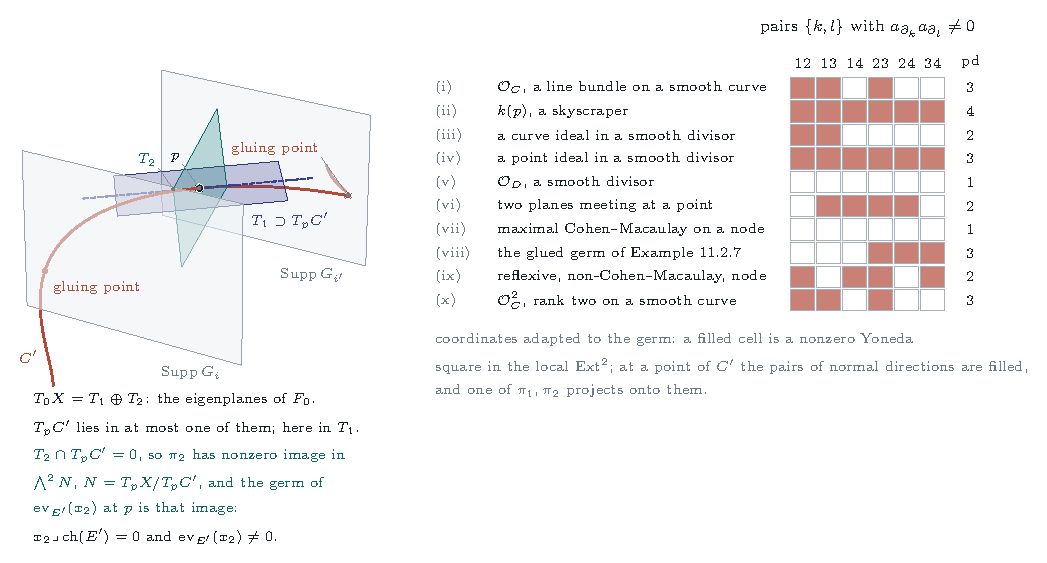
\includegraphics[width=\textwidth]{fig_quarticlocal}
\caption{\Cref{thm:quarticlocal} and \Cref{cor:markmanquarticfails}. Left: the
support of Markman's sheaf $E'$ near a point $p$ of the glued curve $C'$,
between two of the translated supports that the curve crosses at its gluing
points. The tangent space at $p$ is the sum of the eigenplanes $T_{1}$ and
$T_{2}$ of the real multiplication; the tangent line of $C'$ lies in at most
one of them, here in $T_{1}$, so $\pi_{2}$ has nonzero image in
$\bigwedge^{2}N$, $N=T_{p}X/T_{p}C'$, which is the germ of
$\operatorname{ev}_{E'}(x_{2})$ at $p$. Right: for ten germs at the origin
of $\CC^{4}$, the pairs $\{k,l\}$ of coordinate directions whose jet classes
have nonzero product in the local $\Ext^{2}$, and the projective dimension;
rows (i), (ii) and (x) are \Cref{lem:freegerm}, row (iii) is
\Cref{lem:divisorgerm}, row (vi) is \Cref{lem:localproducts}.}
\label{fig:quarticlocal}
\end{figure}

\subsection{Sextic CM fields}\label{ssec:sextic}

The dimension count of \Cref{thm:quarticobstruction} does not extend to CM
fields of degree six, for a reason of parity (\Cref{rem:sexticparity}). Let
$F=F_{0}(\sqrt{-q})$ be a sextic CM field with totally
real cubic subfield $F_{0}$, real places $\tau_{1},\tau_{2},\tau_{3}$ and $q\in
F_{0}$ totally positive, and let $X$ be a principally polarised abelian sixfold
with real multiplication by $\cO_{F_{0}}$, so that
$H^{1}(X,\CC)=U_{1}\oplus U_{2}\oplus U_{3}$ with $U_{j}$ the eigenspace of
$\tau_{j}$, of dimension four and Hodge type $(2,2)$. Let
$\theta_{j}\in H^{1,1}(X)$ be the component of the polarisation on $U_{j}$, so
that $\theta=\sum_{j}\theta_{j}$, $\theta_{j}^{3}=0$ and
$\int_{X}\theta_{1}^{2}\theta_{2}^{2}\theta_{3}^{2}=8$. For $t\in F_{0}$ and
$\varepsilon\in\{\pm1\}^{3}$ put $s_{j}=\sqrt{-1}\,\sqrt{\tau_{j}(q)}$ and
$e_{\varepsilon}=\exp\bigl(\sum_{j}(\tau_{j}(t)+\varepsilon_{j}s_{j})\theta_{j}\bigr)$,
and let $S(t,q)$ be the span of the eight $e_{\varepsilon}$. As in
\Cref{prop:quarticsecant}(i) it is a rational subspace of dimension
$8=2^{[F_{0}:\QQ]}$ of the algebra generated by the $\theta_{j}$, the Galois
group permuting the $e_{\varepsilon}$ as it permutes the CM types of $F$; for
$t=0$ it is the secant space of Markman's construction for $F$ on
$X\times\widehat{X}$ \cite[\S11.1]{Mar25c}, and
$S(t,q)=e^{\sum_{j}\tau_{j}(t)\theta_{j}}S(0,q)$. A real class
$v=\sum_{\varepsilon}w_{\varepsilon}e_{\varepsilon}$ has
$w_{-\varepsilon}=\bbar{w}_{\varepsilon}$. Write $N_{w}$ for the number of
nonzero $w_{\varepsilon}$; $A_{jj'}$ for the number of sign pairs
$(\sigma,\sigma')$ such that $w_{\varepsilon}\ne0$ for some $\varepsilon$ with
$\varepsilon_{j}=\sigma$ and $\varepsilon_{j'}=\sigma'$; $\rho_{j}$ for the rank
of the $2\times4$ matrix $(w_{\varepsilon})$ whose rows are indexed by
$\varepsilon_{j}$ and whose columns by the two other signs; and, for
$\{j,j',j''\}=\{1,2,3\}$ and $\sigma'=\pm1$, $M^{(j;j')}_{\sigma'}$ for the
$2\times2$ matrix $(w_{\varepsilon})_{\varepsilon_{j},\varepsilon_{j''}}$ with
$\varepsilon_{j'}=\sigma'$ fixed. Let $r^{k}(v)$ be the rank of the contraction
$HT^{k}(X)\to H^{*}(X,\CC)$, $\xi\mapsto\xi\lrcorner\,v$.

\begin{proposition}[The count in degree six]\label{prop:sexticcount}
Let $v\in S(t,q)$ be a nonzero real class.
\begin{enumerate}[label=\textup{(\roman*)},leftmargin=2.6em,itemsep=2pt]
\item $r^{1}(v)=12$,
  \[
    r^{2}(v)=4\,(A_{12}+A_{13}+A_{23})+\rho_{1}+\rho_{2}+\rho_{3},
    \qquad
    r^{3}(v)=8N_{w}+2\sum_{j\ne j'}\bigl(\rk M^{(j;j')}_{+}+\rk M^{(j;j')}_{-}\bigr).
  \]
  So $r^{2}(v)\le54$ and $r^{3}(v)\le112$, with equality when every
  $w_{\varepsilon}$ is nonzero and every $M^{(j;j')}_{\sigma'}$ is invertible,
  which holds outside a proper Zariski closed subset of $S(t,q)$. When $F$
  contains an imaginary quadratic field $K$ and $v$ lies in the secant plane
  of $K$, so that $N_{w}=2$, one has $(r^{2},r^{3})=(30,40)$.
\item $\chi(v,v)=\int_{X}v^{\vee}v=-64\,\Nm_{F_{0}/\QQ}(q)\sum_{\varepsilon}
  |w_{\varepsilon}|^{2}<0$. For a CM field of degree $2m$, with $X$ of dimension
  $2m$ and $2^{m}$ exponentials, the same computation gives
  $(-4)^{m}\Nm(q)\sum_{\varepsilon}|w_{\varepsilon}|^{2}$: the Euler form on
  the secant space is definite, of sign $(-1)^{m}$.
\item Let $F_{1},F_{2}$ be perfect complexes on $X$ with
  $\Ext^{<0}(F_{i},F_{i})=0$ and characters $v_{i}$ in spaces
  $S(t_{i},q_{i})$, let $A=X\times\widehat{X}$ carry the action of $F$ of
  \cite[\S11.1]{Mar25c}, transported by the exponential of a rational
  $F_{0}$-$B$-field, and put
  $E=\Phi(F_{1}\boxtimes F_{2}^{\vee})$ and $\kappa=\ch(E)e^{\ell/2}$. Then
  $r(\kappa)=r(\ch E)=r^{2}(v_{1})+144+r^{2}(v_{2})\le252$, while every class
  that stays of Hodge type over $\cD_{F}$ has rank at most
  $\dim HT^{2}(A)-\dim\cD_{F}=276-12=264$. Moreover
  $\dim\Ext^{2}(E,E)\ge r(\kappa)$, with equality if and only if each $F_{i}$
  has
  \[
    \dim\Ext^{k}(F_{i},F_{i})=1,\ 12,\ r^{2}(v_{i}),\ e_{3},\ r^{2}(v_{i}),\ 12,\ 1
    \quad(k=0,\dots,6),
  \]
  where $e_{3}=2r^{2}(v_{i})-22-\chi(v_{i},v_{i})$,
  and this profile is compatible with the bound $e_{3}\ge r^{3}(v_{i})$ exactly
  when $\chi(F_{i},F_{i})\le-(r^{3}(v_{i})-2r^{2}(v_{i})+22)$, that is
  $\chi(F_{i},F_{i})\le-26$ for $v_{i}$ general in its secant space, and
  $\chi(F_{i},F_{i})\le-2$ when $N_{w}=2$.
\item If $t_{1}=t_{2}=0$ and $q_{1}=q_{2}=q$, then $\kappa$ is invariant
  under $G_{F}$, and so is a Hodge class on every member of the
  $(F,2,1)$-family.
\end{enumerate}
\end{proposition}

\begin{proof}
(i) Choose a basis $x_{j1},x_{j2}$ of $U_{j}^{1,0}$ and $y_{j1},y_{j2}$ of
$U_{j}^{0,1}$ with $\theta_{j}=x_{j1}y_{j1}+x_{j2}y_{j2}$, and let
$\omega_{j}=y_{j1}y_{j2}$ span $\bigwedge^{2}U_{j}^{0,1}$. Then
$H^{*}(X,\CC)$ and $HT^{*}(X)=\bigwedge^{*}(H^{0,1}\oplus T)$ are the tensor
products over $j$ of the corresponding algebras of the three factors,
$HT^{k}(X)=\bigoplus_{a_{1}+a_{2}+a_{3}=k}HT^{a_{1}}_{1}\otimes HT^{a_{2}}_{2}
\otimes HT^{a_{3}}_{3}$, and contraction is compatible with the factorisation;
$v=\sum_{\varepsilon}w_{\varepsilon}\bigotimes_{j}e^{\lambda_{j}(\varepsilon_{j})\theta_{j}}$
with $\lambda_{j}(\pm1)=\tau_{j}(t)\pm s_{j}$, two distinct numbers. The blocks
of $HT^{k}(X)$ shift the three Hodge bidegrees of $H^{*}(X)$ by different
amounts, so their images are independent and $r^{k}(v)$ is the sum of their
ranks. Inside a block the bookkeeping rests on two facts about one factor:
the two classes $e^{\lambda_{j}(\pm1)\theta_{j}}$ are linearly independent,
and so are the subspaces $U_{j}^{0,1}e^{\lambda_{j}(\pm1)\theta_{j}}$ of
$H^{*}(U_{j})$, since $u\,e^{\lambda\theta_{j}}=u+\lambda\,u\theta_{j}$ for
$u\in U_{j}^{0,1}$; whereas $\omega_{j}e^{\lambda\theta_{j}}=\omega_{j}$ for
every $\lambda$, so that the summands of a block through $HT^{2}_{j}$ share the
factor $\omega_{j}$ and are combined, not juxtaposed. On one factor,
contraction into $e^{\lambda\theta_{j}}$ is as follows. For $\xi\in HT^{1}_{j}$,
$\xi\lrcorner\,e^{\lambda\theta_{j}}=y^{\lambda}(\xi)\,e^{\lambda\theta_{j}}$ with
$y^{\lambda}(\xi)=\xi^{0,1}+\lambda\,\xi_{T}\lrcorner\,\theta_{j}\in
U_{j}^{0,1}$, as in \Cref{lem:bfield}(i); $y^{\lambda}$ is onto, its kernel
$K^{\lambda}_{j}$ has dimension two, and
$HT^{1}_{j}=K^{\lambda_{j}(+1)}_{j}\oplus K^{\lambda_{j}(-1)}_{j}$ because
$\lambda_{j}(+1)\ne\lambda_{j}(-1)$ and $\xi_{T}\lrcorner\,\theta_{j}$
determines $\xi_{T}$. For $\xi\in HT^{2}_{j}$, since $\omega_{j}\theta_{j}=0$,
one finds $\omega_{j}\lrcorner\,e^{\lambda\theta_{j}}=\omega_{j}$,
$(y_{ja}\otimes\partial_{x_{jb}})\lrcorner\,e^{\lambda\theta_{j}}=\pm\lambda\,
\omega_{j}$ for $a\ne b$ and $0$ for $a=b$, and
$(\partial_{x_{j1}}\wedge\partial_{x_{j2}})\lrcorner\,e^{\lambda\theta_{j}}
=\pm\lambda^{2}\omega_{j}$: the image of $HT^{2}_{j}$ is the line
$\CC\omega_{j}$, $\xi\lrcorner\,e^{\lambda\theta_{j}}=c(\xi,\lambda)\,\omega_{j}$,
and the pairs $\bigl(c(\xi,\lambda_{j}(+1)),c(\xi,\lambda_{j}(-1))\bigr)$ fill
$\CC^{2}$. For $k\ge3$, $HT^{k}_{j}$ kills $e^{\lambda\theta_{j}}$, because
every element of it contains $\omega_{j}$ or $\partial_{x_{j1}}\wedge
\partial_{x_{j2}}$ together with a further factor, and the further factor
kills $\omega_{j}$.

Now count. The block $HT^{1}_{j}$ acts on $v$ by
$\xi\mapsto\sum_{\varepsilon}w_{\varepsilon}\,y^{\lambda_{j}(\varepsilon_{j})}(\xi)
\bigotimes_{j'}e^{\lambda_{j'}(\varepsilon_{j'})\theta_{j'}}$; on the summand
$K^{\lambda_{j}(-\sigma)}_{j}$ only the $\varepsilon$ with
$\varepsilon_{j}=\sigma$ contribute, and they map it isomorphically onto
$U_{j}^{0,1}$ tensored with a nonzero class as soon as one such
$w_{\varepsilon}$ is nonzero. Both signs occur in the support of a nonzero real
$w$, since $w_{-\varepsilon}=\bbar{w}_{\varepsilon}$, so the block has rank $4$
and $r^{1}(v)=12$. The block $HT^{1}_{j}\otimes HT^{1}_{j'}$ is the sum of the
four summands $K^{\lambda_{j}(-\sigma)}_{j}\otimes K^{\lambda_{j'}(-\sigma')}_{j'}$,
each of dimension four; the summand indexed by $(\sigma,\sigma')$ maps
isomorphically onto $U_{j}^{0,1}\otimes U_{j'}^{0,1}$ tensored with the class
$\sum_{\sigma''}w_{\varepsilon}e^{\lambda_{j''}(\sigma'')\theta_{j''}}$, which
is nonzero exactly when the pair $(\sigma,\sigma')$ occurs in the support, and
to zero otherwise; so the block has rank $4A_{jj'}$. The block $HT^{2}_{j}$
maps $\xi$ to $\sum_{\sigma}c(\xi,\lambda_{j}(\sigma))\,z_{\sigma}$ with
$z_{\sigma}=\omega_{j}\otimes\sum_{\mu}w_{\sigma\mu}e_{\mu}$, where $\mu$ runs
over the four sign patterns of the other two places and the $e_{\mu}$ are
independent; as $(c(\xi,\lambda_{j}(+1)),c(\xi,\lambda_{j}(-1)))$ fills
$\CC^{2}$, the rank is the dimension of the span of $z_{+},z_{-}$, which is
$\rho_{j}$. This gives $r^{2}(v)$. In degree three the block
$HT^{1}_{1}\otimes HT^{1}_{2}\otimes HT^{1}_{3}$ is the sum of eight summands
$\bigotimes_{j}K^{\lambda_{j}(-\varepsilon_{j})}_{j}$, of dimension eight, on
each of which exactly one term of $v$ acts, isomorphically when
$w_{\varepsilon}\ne0$ and by zero otherwise: rank $8N_{w}$. The block
$HT^{2}_{j}\otimes HT^{1}_{j'}$ factors through $\CC^{2}\otimes HT^{1}_{j'}$
by $c\otimes\mathrm{id}$, which is onto, and on
$\CC^{2}\otimes K^{\lambda_{j'}(-\sigma')}_{j'}$ the map is
$M^{(j;j')}_{\sigma'}\otimes y^{\lambda_{j'}(\sigma')}$ followed by tensoring
with independent classes, of rank $2\rk M^{(j;j')}_{\sigma'}$; the two values
of $\sigma'$ give independent images. The blocks $HT^{3}_{j}$ contribute
nothing. This gives $r^{3}(v)$. The maximal values are $48+6=54$ and
$64+6\cdot8=112$; the conditions for them are the nonvanishing of the
$w_{\varepsilon}$ and of the determinants of the $M^{(j;j')}_{\sigma'}$, which
are polynomials in the coordinates of $v$, nonzero on $S(t,q)$. If $F\supseteq K$
and $v$ lies in the secant plane of $K$, the support of $w$ is a pair
$\{\varepsilon_{0},-\varepsilon_{0}\}$, the two CM types of $F$ induced from
$K$; then $A_{jj'}=2$, $\rho_{j}=2$, $N_{w}=2$ and every
$M^{(j;j')}_{\sigma'}$ has one nonzero entry, so $(r^{2},r^{3})=(24+6,16+24)$.

(ii) Since $\theta_{j}^{3}=0$, $\theta^{2m}=\frac{(2m)!}{2^{m}}\theta_{1}^{2}
\cdots\theta_{m}^{2}$, and $\int_{X}\theta^{2m}/(2m)!=1$ gives
$\int_{X}\theta_{1}^{2}\cdots\theta_{m}^{2}=2^{m}$ and
$\int_{X}\exp(\sum_{j}c_{j}\theta_{j})=\prod_{j}c_{j}^{2}$. The dual of
$e^{\lambda\theta_{j}}$ is $e^{-\lambda\theta_{j}}$, so
$\int_{X}e_{\varepsilon}^{\vee}e_{\varepsilon'}=\prod_{j}\bigl(\lambda_{j}(\varepsilon'_{j})
-\lambda_{j}(\varepsilon_{j})\bigr)^{2}$, which is $0$ unless
$\varepsilon'=-\varepsilon$, where it is $\prod_{j}(2s_{j})^{2}=(-4)^{m}\Nm(q)$.
Hence $\chi(v,v)=(-4)^{m}\Nm(q)\sum_{\varepsilon}w_{\varepsilon}w_{-\varepsilon}
=(-4)^{m}\Nm(q)\sum_{\varepsilon}|w_{\varepsilon}|^{2}$.

(iii) As in the proof of \Cref{thm:quarticobstruction}(i), $r(\kappa)=r(\ch E)$
by \Cref{lem:bfield}(i), and $\Phi$ identifies $r(\ch E)$ with the rank of
contraction from $HT^{2}(X\times X)=\bigoplus_{a+b=2}HT^{a}(X)\otimes HT^{b}(X)$
into $v_{1}\boxtimes v_{2}$; the block $HT^{1}\otimes HT^{1}$ contributes
$r^{1}(v_{1})r^{1}(v_{2})=144$ and the other two contribute
$r^{2}(v_{1})+r^{2}(v_{2})$, by the type argument given there. The tangent
space $T_{[A]}\cD_{F}\subseteq H^{1}(T_{A})$, of dimension $mn^{2}=12$, kills
every class that stays of Hodge type along $\cD_{F}$, as in
\Cref{prop:p2primelocus}(i), and $\dim HT^{2}(A)=66+144+66$. By the K\"unneth
formula, with $\Ext^{<0}=0$,
$\dim\Ext^{2}(E,E)=e_{0}e_{2}'+e_{1}e_{1}'+e_{2}e_{0}'$ where
$e_{k}=\dim\Ext^{k}(F_{1},F_{1})$ and $e_{k}'=\dim\Ext^{k}(F_{2},F_{2})$; the
commutative square $\sigma\circ\operatorname{ev}=(\,\cdot\,)\lrcorner\ch$ of
\Cref{setup:criterion}, valid in every degree, gives $e_{k}\ge r^{k}(v_{1})$
and $e_{k}'\ge r^{k}(v_{2})$, and $e_{0},e_{0}'\ge1$. So
$\dim\Ext^{2}(E,E)\ge r^{2}(v_{2})+144+r^{2}(v_{1})$, with equality if and
only if $e_{0}=e_{0}'=1$, $e_{1}=e_{1}'=12$, $e_{2}=r^{2}(v_{1})$ and
$e_{2}'=r^{2}(v_{2})$. Serre duality on the sixfold gives $e_{k}=e_{6-k}$, so
$\chi(F_{i},F_{i})=2(e_{0}-e_{1}+e_{2})-e_{3}=2r^{2}(v_{i})-22-e_{3}$, and by
Riemann--Roch on an abelian variety $\chi(F_{i},F_{i})=\chi(v_{i},v_{i})$,
which is (ii); this determines $e_{3}$, and $e_{3}\ge r^{3}(v_{i})$ is the
stated inequality. With the maximal ranks it reads
$\chi\le-(112-108+22)=-26$, and with $N_{w}=2$ it reads
$\chi\le-(40-60+22)=-2$.

(iv) The proof of \Cref{thm:quarticobstruction}(iii) applies with three
factors in place of two: for $t=0$ the classes $e_{\varepsilon}\boxtimes
e_{\varepsilon'}^{\vee}$, the correspondence $Z\mapsto\ch(\Phi(Z))e^{\ell/2}$
and the Poincar\'e class decompose as tensor products over $j$ of classes of
even degree, on each factor $\sqrt{-q}$ acts as in the imaginary quadratic
construction with $d$ replaced by $\tau_{j}(q)$, and the identities of
\Cref{prop:flatall} at $n=2$ show that each image is a multiple of an
exponential of $\eta_{j}$ or of a Weil class of the $j$-th factor, invariant
under the special unitary group of that factor; $G_{F}(\RR)$ is the product of
the three, and is Zariski dense in $G_{F}$. Statement (iv) is the case
$[F:\QQ]=6$ of \cite[Proposition~10.2.1(1)]{Mar25c}, with the inclusion
$\widetilde\phi(B\otimes B)\subset A$ of \cite[p.~33]{Mar25c}, which Markman
proves for every CM field in his conventions for $\Phi$ and for the twist; we
make no claim of priority.
\end{proof}

\begin{remark}[The special role of degree four]
\label{rem:sexticparity}
In \Cref{thm:quarticobstruction} the equality $\dim\Ext^{2}(E,E)=r(\kappa)$
determines the whole Ext profile of each factor, because on a fourfold
$\Ext^{2}$ is the middle degree and Serre duality supplies the rest; the Euler
characteristic of a minimal factor is then the small positive integer
$r^{2}-14$, the Euler form on the secant space being positive definite, and
the arithmetic of \Cref{prop:quarticother} excludes it. On a sixfold the same
equality fixes $\Ext^{0}$, $\Ext^{1}$ and $\Ext^{2}$ and leaves the middle
group $\Ext^{3}$ free, and the Euler form has the opposite sign:
$\chi(F_{i},F_{i})=-64\Nm(q)\sum|w_{\varepsilon}|^{2}$ is a negative integer
that $e_{3}$ absorbs. So no dimension count excludes a minimal Orlov product
over a sextic field, and none does over any CM field of degree $2m\ge6$,
where $\Ext^{3},\dots,\Ext^{m}$ are free and the Euler form has sign
$(-1)^{m}$. What \Cref{prop:sexticcount}(iii) leaves for such an object is the
profile displayed there, with $\chi(F_{i},F_{i})\le-26$ for a general secant
character, and the flat twisted character of (iv), which stays of Hodge type
over the whole twelve-dimensional period domain. Whether a sheaf with that
profile exists on a sixfold with real multiplication by a cubic field is not
known; nothing in \Cref{thm:quarticobstruction} bears on it. A certificate
of the kind of \Cref{thm:twistedcert} for a sextic field would be an Orlov
product of such sheaves, with $\dim\Ext^{2}(E,E)=r(\kappa)\le252$ on the
twelvefold, whose twisted character has a nonzero component in the Weil
classes $W_{F}(A)$; flatness does not give that component, and
\Cref{lem:sexticweil} computes it. In degree six as in degree four, the Orlov
products never reach the rank of a class of general shape: $r(\kappa)\le252$
against $264$, and $r(\kappa)\le104$ against $112$.
\end{remark}

The count of \Cref{prop:sexticcount}(iii) is a condition on the Euler
characteristic of the character alone, so it can be tested on the lattice of
integral characters, as \Cref{prop:quarticother} tests the quartic one. In
degree four the test excludes every minimal character. In degree six it can
exclude an integral character only if $-26<\chi(v,v)<0$
(\Cref{prop:sexticintegral}(i),(ii)), and it excludes neither of the integral
classes $\operatorname{Re}e^{\sqrt{-1}\,\theta}$ and
$\operatorname{Im}e^{\sqrt{-1}\,\theta}$ (\Cref{prop:sexticintegral}(iv)). For
$t=0$, the case in which
\Cref{prop:sexticcount}(iv) makes $\kappa$ flat, put
$B_{j}=1-\tfrac12\tau_{j}(q)\,\theta_{j}^{2}$, so that
$e^{\pm s_{j}\theta_{j}}=B_{j}\pm s_{j}\theta_{j}$, and for
$c_{0},c_{3}\in\QQ$ and $f,g\in F_{0}$ let
\[
  v(c_{0},f,g,c_{3})=c_{0}B_{1}B_{2}B_{3}
  +\sum_{j}\tau_{j}(f)\,\theta_{j}B_{k}B_{l}
  +\sum_{j}\tau_{j}(g)\,B_{j}\theta_{k}\theta_{l}
  +c_{3}\,\theta_{1}\theta_{2}\theta_{3},
\]
where $\{j,k,l\}=\{1,2,3\}$ in each sum.

\begin{proposition}[Integral flat characters in degree six]
\label{prop:sexticintegral}
Keep the notation of \Cref{prop:sexticcount}.
\begin{enumerate}[label=\textup{(\roman*)},leftmargin=2.6em,itemsep=2pt]
\item For every perfect complex $F$ on a complex torus of dimension six,
  $\chi(F,F)$ is even. So the condition of \Cref{prop:sexticcount}(iii)
  holds for every $F$ whose character has $N_{w}=2$.
\item For every nonzero real $v\in S(t,q)$, $r^{3}(v)-2r^{2}(v)\le4$, with
  equality only if $(r^{2}(v),r^{3}(v))=(54,112)$. So for every shape the
  condition of \Cref{prop:sexticcount}(iii) is implied by
  $\chi(F_{i},F_{i})\le-26$.
\item The rational points of $S(0,q)$ are the classes $v(c_{0},f,g,c_{3})$,
  and
  \[
    \chi(v,v)=-8\bigl(\Nm(q)\,c_{0}^{2}+\Tr\bigl(\Nm(q)\,q^{-1}f^{2}\bigr)
    +\Tr(q\,g^{2})+c_{3}^{2}\bigr).
  \]
\item For $q=1$, the classes $\operatorname{Re}e^{\sqrt{-1}\,\theta}=v(1,0,-1,0)$
  and $\operatorname{Im}e^{\sqrt{-1}\,\theta}=v(0,1,0,-1)$ are integral
  points of $S(0,1)$ with $\chi=-32$ and $N_{w}=2$, so they satisfy the
  condition of \Cref{prop:sexticcount}(iii).
\end{enumerate}
\end{proposition}

\begin{proof}
(i) The Chern character $v=\ch(F)$ is integral, as in the proof of
\Cref{thm:quarticobstruction}(ii), and $\chi(F,F)=\int_{X}v^{\vee}v$ by
Riemann--Roch. Write $v=\sum_{k}v_{2k}$, so that
$\int_{X}v^{\vee}v=\sum_{k}(-1)^{k}\int_{X}v_{2k}v_{12-2k}$. The terms $k$ and
$6-k$ are equal, since $(-1)^{k}=(-1)^{6-k}$ and classes of even degree
commute, so they contribute an even number when $k\ne3$. For $k=3$ write
$v_{6}=\sum_{I}a_{I}e_{I}$ in the basis of $\bigwedge^{6}H^{1}(X,\ZZ)$ given
by the products $e_{I}$ of six elements of a basis of $H^{1}(X,\ZZ)$; since
$e_{I}e_{I}=0$ and $e_{I}e_{J}=e_{J}e_{I}$, $v_{6}^{2}=2\sum_{I<J}a_{I}a_{J}
e_{I}e_{J}$ is even. For $N_{w}=2$ the condition of
\Cref{prop:sexticcount}(iii) is $\chi(F,F)\le-2$, and $\chi(F,F)$ is a
negative even integer by \Cref{prop:sexticcount}(ii).

(ii) For $j$ and $\sigma=\pm1$ let $W_{j,\sigma}$ be the $2\times2$ slice
$(w_{\varepsilon})_{\varepsilon_{j}=\sigma}$, with rows and columns indexed by
the signs at the two other places. The matrices $M^{(j';j)}_{\sigma}$ are
$W_{j,\sigma}$ and its transpose, so
$\sum_{j\ne j'}\bigl(\rk M^{(j;j')}_{+}+\rk M^{(j;j')}_{-}\bigr)
=2\sum_{j,\sigma}\rk W_{j,\sigma}$. Since $w_{-\varepsilon}=\bbar{w}_{\varepsilon}$,
$W_{j,-}$ is the complex conjugate of $W_{j,+}$ with its rows and its columns
reversed, so the two slices have the same rank $k_{j}$. Let $S$ be the support
of $w$ and $N=N_{w}=|S|$. By \Cref{prop:sexticcount}(i),
\begin{equation}\label{eq:sexticexcess}
  r^{3}(v)-2r^{2}(v)=8N-8\,(A_{12}+A_{13}+A_{23})
  +\sum_{j}\bigl(8k_{j}-2\rho_{j}\bigr).
\end{equation}
The set $S$ is stable under $\varepsilon\mapsto-\varepsilon$, which exchanges
the two slices along each place; so $N$ is even, each slice has $N/2$ nonzero
entries, $k_{j}\ge1$, and $A_{jj'}\in\{2,4\}$, the projection of $S$ to the
signs at $j$ and $j'$ being stable under negation. Also $1\le\rho_{j}\le2$ and
$k_{j}\le2$, and a slice whose nonzero entries lie in one row or one column
has rank one. If $\rho_{j}=1$, then $w_{\varepsilon}=a_{\varepsilon_{j}}
W(\varepsilon')$, with $\varepsilon'$ the signs at the two other places, so
every slice along a place $j'\ne j$ is $a\otimes(\text{a row of }W)$ and
$k_{j'}\le1$. Now take the four values of $N$ in turn.

If $N=8$, every $A_{jj'}$ is $4$ and \eqref{eq:sexticexcess} is
$-32+\sum_{j}(8k_{j}-2\rho_{j})$. When every $\rho_{j}$ is $2$ this is at most
$-32+3\cdot12=4$, with equality exactly when every $k_{j}$ is $2$, and then
$r^{2}=48+6=54$ and $r^{3}=64+48=112$. When some $\rho_{j}$ is $1$, the two
other $k$ are at most $1$ and \eqref{eq:sexticexcess} is at most
$-32+14+6+6=-6$.

If $N=6$, $S$ misses one pair $\{\pm\varepsilon_{0}\}$. As $\varepsilon_{0}$
and $-\varepsilon_{0}$ differ at every place, they never have the same signs
at two places, so every sign pair at two places occurs in $S$, every
$A_{jj'}$ is $4$, and \eqref{eq:sexticexcess} is at most $48-96+3\cdot14=-6$.

If $N=4$, $S=\{\pm\varepsilon,\pm\varepsilon'\}$, and after replacing
$\varepsilon'$ by $-\varepsilon'$ if necessary, $\varepsilon$ and
$\varepsilon'$ differ at exactly one place $j$. For the two other places $k$
and $l$ one has $A_{kl}=2$ and $A_{jk}=A_{jl}=4$. The two nonzero entries of
a slice along $k$ are $w_{\pm\varepsilon}$ and $w_{\pm\varepsilon'}$ with the
same sign, whose indices agree at $l$; they lie in one row or one column, so
$k_{k}=1$, and likewise $k_{l}=1$. Hence \eqref{eq:sexticexcess} is at most
$32-80+8\,(2+1+1)-6=-22$.

If $N=2$, $S=\{\pm\varepsilon_{0}\}$, every $A_{jj'}$ is $2$, every $k_{j}$ is
$1$, and every $\rho_{j}$ is $2$, the two slices along $j$ having their
nonzero entries at different positions; so \eqref{eq:sexticexcess} is
$16-48+24-12=-20$, the value $40-60$ of \Cref{prop:sexticcount}(i).

So $r^{3}-2r^{2}\le4$, with equality only at $(54,112)$, and the threshold
$r^{3}-2r^{2}+22$ of \Cref{prop:sexticcount}(iii) is at most $26$.

(iii) Since $\theta_{j}^{3}=0$ and $s_{j}^{2}=-\tau_{j}(q)$,
$e^{\pm s_{j}\theta_{j}}=B_{j}\pm s_{j}\theta_{j}$, so the eight exponentials
and the eight products $\prod_{j}\beta_{j}$ with $\beta_{j}\in\{B_{j},\theta_{j}\}$
span the same complex space, the change of basis being the tensor cube of an
invertible $2\times2$ matrix. The Galois group permutes the $\tau_{j}$, the
$\theta_{j}$ and the $B_{j}$ compatibly, so $\sum_{a}C_{a}\prod_{j}\beta_{j}$,
indexed by the subsets $a$ of $\{1,2,3\}$ with $\beta_{j}=\theta_{j}$ for
$j\in a$, is rational exactly when $C_{\pi(a)}=\sigma(C_{a})$ for every
$\sigma$ inducing $\pi$; the stabiliser of $\{j\}$, and of its complement,
is the stabiliser of $\tau_{j}$, which gives the form $v(c_{0},f,g,c_{3})$.
The involution $v\mapsto v^{\vee}$ and the integral are multiplicative over
the three factors, with $\int_{X}\theta_{1}^{2}\theta_{2}^{2}\theta_{3}^{2}=8$;
on one factor $B_{j}^{\vee}B_{j}=1-\tau_{j}(q)\theta_{j}^{2}$,
$\theta_{j}^{\vee}\theta_{j}=-\theta_{j}^{2}$ and the mixed products are odd
in $\theta_{j}$. So
$\chi(v,v)=-8\sum_{a}C_{a}^{2}\prod_{j\notin a}\tau_{j}(q)$, which is the
formula.

(iv) For $q=1$, $s_{j}=\sqrt{-1}$ and $e_{(1,1,1)}=\prod_{j}e^{\sqrt{-1}\,
\theta_{j}}=e^{\sqrt{-1}\,\theta}$. The polarisation is principal, so each
$\theta^{k}/k!$ is integral, and so are the real and imaginary parts
$\sum_{k}(-1)^{k}\theta^{2k}/(2k)!$ and $\sum_{k}(-1)^{k}\theta^{2k+1}/(2k+1)!$.
They are $\tfrac12(e_{(1,1,1)}+e_{(-1,-1,-1)})$ and
$\tfrac1{2\sqrt{-1}}(e_{(1,1,1)}-e_{(-1,-1,-1)})$, so $N_{w}=2$ and
$\chi=-64\,(\tfrac14+\tfrac14)=-32$ by \Cref{prop:sexticcount}(ii); expanding
$\prod_{j}(B_{j}+\sqrt{-1}\,\theta_{j})$ gives the coordinates.
\end{proof}

The flatness of \Cref{prop:sexticcount}(iv) makes $\kappa$ a Hodge class on
every member of the family, but in degree four the Hodge classes of a very
general member are the products of divisor classes and the Weil classes
$W_{F}(A)$ (\Cref{prop:cmweil}(iii)), and only a nonzero component of
$\kappa$ in $W_{F}(A)$ bears on $\mathbf{W}(F,2,1)$. We compute that
component. Keep the notation of \Cref{prop:sexticcount}, with $t_{1}=t_{2}=0$,
$q_{1}=q_{2}=q$ and trivial $B$-field, put $d_{j}=\tau_{j}(q)$, and let
$\Psi(Z)=\ch(\Phi(Z))e^{\ell/2}$ as in \Cref{prop:flatall}, so that
$\kappa(v_{1},v_{2})=\Psi(v_{1}\boxtimes v_{2}^{\vee})$ for the characters
$v_{i}$ of $F_{i}$. As in the proof of \Cref{prop:sexticcount}(iv),
$H^{1}(A,\CC)$ is the sum of three factors $U_{j}\oplus U_{j}^{\vee}$, on each
of which $\sqrt{-q}$ acts as in the imaginary quadratic construction with
$\beta=\theta_{j}$ and $d=d_{j}$. On the $j$-th factor write
$\widehat\theta_{j}$ and $\ell_{j}$ for the components of the dual
polarisation and of the Poincar\'e class, and put
$\gamma_{j}=d_{j}\theta_{j}-\widehat\theta_{j}$, as in \eqref{eq:gammadef},
and $\eta_{j}=d_{j}\theta_{j}+\widehat\theta_{j}$, a positive multiple of the
polarisation of the factor for which $\sqrt{-q}$ is anti-self-adjoint
(\Cref{prop:splitgeom}(i)). For $\sigma=\pm1$ let $\tau_{j,\sigma}$ be the
embedding of $F$ over $\tau_{j}$ with
$\tau_{j,\sigma}(\sqrt{-q})=\sigma\sqrt{-1}\,\sqrt{\tau_{j}(q)}=\sigma s_{j}$,
and $V_{j,\sigma}\subset H^{1}(A,\CC)$ its eigenspace, of dimension four. By
\Cref{thm:splitclosed}(ii) with $n=2$ and $d=d_{j}$, the line
$\bigwedge^{4}V_{j,\sigma}$ is spanned by
\begin{equation}\label{eq:sexticomega}
  \omega_{j,\sigma}=-\frac{1}{2d_{j}^{2}}\bigl(\gamma_{j}-\sigma s_{j}\ell_{j}\bigr)^{2},
\end{equation}
so the six classes $\omega_{j,\sigma}$ span $W_{F}(A)\otimes\CC$. Since
$\eta_{j}$ pairs $V_{j,+}$ with $V_{j,-}$, the products $\eta_{i}\eta_{k}$ lie
in summands of $H^{4}(A,\CC)=\bigwedge^{4}\bigl(\bigoplus_{j,\sigma}
V_{j,\sigma}\bigr)$ other than the six lines $\bigwedge^{4}V_{j,\sigma}$. Let
$\kappa_{j,\sigma}(v_{1},v_{2})$ be the coefficient of $\omega_{j,\sigma}$ in
the component of $\kappa(v_{1},v_{2})$ in $\bigwedge^{4}V_{j,\sigma}$; the
\emph{$F$-Weil part} of $\kappa$ is
$\sum_{j,\sigma}\kappa_{j,\sigma}\,\omega_{j,\sigma}$, its component in
$W_{F}(A)\otimes\CC$. For $\varepsilon\in\{\pm1\}^{3}$ let
$\varepsilon^{(j)}$ be the sign vector that agrees with $\varepsilon$ at $j$
and only there.

\begin{lemma}[The $F$-Weil part of an Orlov product]\label{lem:sexticweil}
Let $v_{i}=\sum_{\varepsilon}w^{i}_{\varepsilon}e_{\varepsilon}\in S(0,q)$ for
$i=1,2$.
\begin{enumerate}[label=\textup{(\roman*)},leftmargin=2.6em,itemsep=2pt]
\item The degree-four part of $\kappa(v_{1},v_{2})$ is a quadratic form in the
  $\eta_{j}$ plus $\sum_{j,\sigma}\kappa_{j,\sigma}\,\omega_{j,\sigma}$, with
  \[
    \kappa_{j,\sigma}(v_{1},v_{2})=-16\Nm(q)\,\tau_{j}(q)
    \sum_{\varepsilon_{j}=\sigma}w^{1}_{\varepsilon}\,w^{2}_{\varepsilon^{(j)}}.
  \]
\item Let $v=v(c_{0},f,g,c_{3})$ be rational, and for $\{j,k,l\}=\{1,2,3\}$
  write $f_{j}=\tau_{j}(f)$, $g_{j}=\tau_{j}(g)$ and $q_{j}=\tau_{j}(q)$. The
  numbers
  \begin{align*}
    R_{j}&=c_{0}^{2}+\frac{f_{k}^{2}}{q_{k}}+\frac{f_{l}^{2}}{q_{l}}
      +\frac{g_{j}^{2}}{q_{k}q_{l}}-\frac{1}{q_{j}}\Bigl(f_{j}^{2}
      +\frac{g_{l}^{2}}{q_{k}}+\frac{g_{k}^{2}}{q_{l}}
      +\frac{c_{3}^{2}}{q_{k}q_{l}}\Bigr),\\
    I_{j}&=c_{0}f_{j}+\frac{f_{k}g_{l}}{q_{k}}+\frac{f_{l}g_{k}}{q_{l}}
      +\frac{c_{3}g_{j}}{q_{k}q_{l}}
  \end{align*}
  are $\tau_{j}(R)$ and $\tau_{j}(I)$ for elements $R,I\in F_{0}$. Put
  $\Omega(v)=R+2I/\sqrt{-q}\in F$. Then
  \[
    \kappa_{j,\sigma}(v,v)=-\Nm(q)\,\tau_{j}(q)\,\tau_{j,\sigma}\bigl(\Omega(v)\bigr).
  \]
  So the $F$-Weil part of $\kappa(v,v)$ is zero if $R=I=0$, and otherwise
  all six $\kappa_{j,\sigma}(v,v)$ are nonzero.
\item If $v_{1}$ and $v_{2}$ are supported on one pair
  $\{\varepsilon_{0},-\varepsilon_{0}\}$, the $F$-Weil part of
  $\kappa(v_{1},v_{2})$ is zero. For $q=1$, $F$ contains
  $K=\QQ(\sqrt{-1})$, the classes $\operatorname{Re}e^{\sqrt{-1}\,\theta}$ and
  $\operatorname{Im}e^{\sqrt{-1}\,\theta}$ span the plane $P_{\theta}$ of
  \Cref{def:secantplane} with $d=1$, and for
  $v_{i}=a_{i}\operatorname{Re}e^{\sqrt{-1}\,\theta}
  +b_{i}\operatorname{Im}e^{\sqrt{-1}\,\theta}$ with $a_{i},b_{i}\in\QQ$ the
  class $\kappa(v_{1},v_{2})$ lies in $\QQ[\eta]\oplus W_{K}(A)$, where
  $\eta=\theta+\widehat\theta$ and $W_{K}(A)\subseteq H^{12}(A,\QQ)$ are the
  Weil classes of $K$ on the twelvefold (\Cref{prop:composite}); its part of
  degree at most four is
  \[
    -32(a_{1}a_{2}+b_{1}b_{2})+16(a_{1}b_{2}-a_{2}b_{1})\,\eta
    +4(a_{1}a_{2}+b_{1}b_{2})\,\eta^{2}.
  \]
\end{enumerate}
\end{lemma}

\begin{proof}
(i) The classes $e_{\varepsilon}\boxtimes e_{\varepsilon'}^{\vee}
=\bigotimes_{j}\bigl(e^{\varepsilon_{j}s_{j}\theta_{j}}\boxtimes
e^{-\varepsilon'_{j}s_{j}\theta_{j}}\bigr)$ and $\Psi$ decompose over the three
factors, as in the proof of \Cref{prop:sexticcount}(iv), and on the $j$-th
factor the two identities of \Cref{prop:flatall} at $n=2$ read, with their
constants,
\[
  \Psi_{j}\bigl(e^{\sigma s_{j}\theta_{j}}\boxtimes e^{\sigma s_{j}\theta_{j}}\bigr)
  =-4d_{j}\,e^{\sigma(s_{j}/2d_{j})\eta_{j}},
  \qquad
  \Psi_{j}\bigl(e^{\sigma s_{j}\theta_{j}}\boxtimes e^{-\sigma s_{j}\theta_{j}}\bigr)
  =\tfrac12\bigl(\gamma_{j}-\sigma s_{j}\ell_{j}\bigr)^{2}
  =-d_{j}^{2}\,\omega_{j,\sigma},
\]
since $s_{j}^{2}=-d_{j}$. So
$\Psi(e_{\varepsilon}\boxtimes e_{\varepsilon'}^{\vee})$ is the product over
$j$ of the first class where $\varepsilon'_{j}=-\varepsilon_{j}$ and of the
second where $\varepsilon'_{j}=\varepsilon_{j}$. In degree four a product with
two or three factors of the second kind vanishes, one with none is a
quadratic form in the $\eta_{j}$, and one with exactly one, at $j$, has
$\varepsilon'=\varepsilon^{(j)}$ and equals
$-d_{j}^{2}\prod_{i\ne j}(-4d_{i})\,\omega_{j,\varepsilon_{j}}
=-16\Nm(q)\,d_{j}\,\omega_{j,\varepsilon_{j}}$. Summing
$w^{1}_{\varepsilon}w^{2}_{\varepsilon'}\Psi(e_{\varepsilon}\boxtimes
e_{\varepsilon'}^{\vee})$ over $\varepsilon$ and $\varepsilon'$ gives (i).

(ii) An element $h$ of the Galois group that fixes the place $j$ permutes
the two others, so it fixes $R_{j}$ and $I_{j}$, which are symmetric in $k$
and $l$; hence $R_{j},I_{j}\in\tau_{j}(F_{0})$, and moving $j$ by the Galois
group shows that they are the conjugates of two elements of $F_{0}$. Write
$\varepsilon=(\sigma,\mu)$ with $\mu$ the signs at $k$ and $l$, so that
$\varepsilon^{(j)}=(\sigma,-\mu)$. Since $e^{\pm s_{i}\theta_{i}}=B_{i}\pm
s_{i}\theta_{i}$, the class $v=\sum_{a}C_{a}\prod_{i\in a}\theta_{i}
\prod_{i\notin a}B_{i}$, with $C_{\emptyset}=c_{0}$, $C_{\{i\}}=f_{i}$,
$C_{\{1,2,3\}\setminus\{i\}}=g_{i}$ and $C_{\{1,2,3\}}=c_{3}$, has
$w_{\varepsilon}=\frac18\sum_{a}C_{a}\prod_{i\in a}\varepsilon_{i}/s_{i}$.
Grouping $a=b$ and $a=b\cup\{j\}$ for $b\subseteq\{k,l\}$ gives
$w_{(\sigma,\mu)}=\frac18\sum_{b}D_{b}\prod_{i\in b}\mu_{i}/s_{i}$ with
$D_{b}=C_{b}+u\,C_{b\cup\{j\}}$ and $u=\sigma/s_{j}=\tau_{j,\sigma}(1/\sqrt{-q})$.
Since $\sum_{\mu}\prod_{i\in b}\mu_{i}\prod_{i\in b'}(-\mu_{i})
=4(-1)^{|b|}\delta_{bb'}$ and $s_{i}^{2}=-q_{i}$,
\[
  \sum_{\varepsilon_{j}=\sigma}w_{\varepsilon}w_{\varepsilon^{(j)}}
  =\frac1{16}\Bigl((c_{0}+uf_{j})^{2}+\frac{(f_{k}+ug_{l})^{2}}{q_{k}}
  +\frac{(f_{l}+ug_{k})^{2}}{q_{l}}+\frac{(g_{j}+uc_{3})^{2}}{q_{k}q_{l}}\Bigr),
\]
and expanding with $u^{2}=-1/q_{j}$ gives $\frac1{16}(R_{j}+2uI_{j})
=\frac1{16}\tau_{j,\sigma}(\Omega(v))$. With (i) this is the formula. The
embedding $\tau_{j,\sigma}$ is injective and $1$, $1/\sqrt{-q}$ are
independent over $F_{0}$, so one $\kappa_{j,\sigma}(v,v)$ vanishes if and only
if $R=I=0$, and then all do.

(iii) If $w^{1}$ and $w^{2}$ vanish off $\{\varepsilon_{0},-\varepsilon_{0}\}$,
no term of (i) survives, since $\varepsilon^{(j)}$ is neither $\varepsilon$
nor $-\varepsilon$. For $q=1$, $s_{j}=\sqrt{-1}$ and
$e_{(1,1,1)}=e^{\sqrt{-1}\,\theta}$, whose real and imaginary parts are
$u_{\theta}$ and $v_{\theta}$ of \eqref{eq:uv} with $d=1$, supported on
$\{\pm(1,1,1)\}$. On each factor $\sqrt{-1}=\sqrt{-q}$ acts as in the
imaginary quadratic construction with $\beta=\theta_{j}$ and $d=1$, so $K$
acts on $A$ by the action \eqref{eq:Mdef} determined by $\theta$ with $d=1$,
and \Cref{prop:flatall} with $n=6$ and $d=1$ gives
$\kappa\in\QQ[\eta]\oplus W_{K}(A)$. For the constants write
$v_{1}=w_{1}e^{\sqrt{-1}\,\theta}+\bbar w_{1}e^{-\sqrt{-1}\,\theta}$ and
$v_{2}^{\vee}=a_{2}\operatorname{Re}e^{\sqrt{-1}\,\theta}
-b_{2}\operatorname{Im}e^{\sqrt{-1}\,\theta}
=w_{2}e^{\sqrt{-1}\,\theta}+\bbar w_{2}e^{-\sqrt{-1}\,\theta}$, with
$w_{1}=\frac12(a_{1}-\sqrt{-1}\,b_{1})$ and $w_{2}=\frac12(a_{2}+\sqrt{-1}\,
b_{2})$. By the first identity in the proof of (i),
$\Psi(e^{\pm\sqrt{-1}\,\theta}\boxtimes e^{\pm\sqrt{-1}\,\theta})
=-64\,e^{\pm(\sqrt{-1}/2)\eta}$, while the two mixed terms have degree
twelve; so in degrees below twelve $\kappa$ is
$-128\operatorname{Re}\bigl(w_{1}w_{2}\,e^{(\sqrt{-1}/2)\eta}\bigr)$, whose
terms of degree $0$, $2$ and $4$ are the stated ones.
\end{proof}

Markman states his reduction for the normalised class
$\ch(E)\exp(-c_{1}(E)/\rk E)$, and it is the component of degree four of that
class, a polynomial in the invariant divisor classes plus a Weil class, whose
algebraicity on the deformations he needs \cite[Proposition~10.2.1,
Corollary~10.2.3]{Mar25c}. When $\rk E\ne0$ that class is
$\kappa\exp(-\kappa_{1}/\rk E)$, with $\kappa_{1}$ the degree-two part of
$\kappa$, which is a linear form in the $\eta_{j}$ by the proof of
\Cref{lem:sexticweil}(i); so it has the same $F$-Weil part as $\kappa$.

For $q=1$ the Orlov products of complexes with characters in
$\QQ\operatorname{Re}e^{\sqrt{-1}\,\theta}\oplus\QQ\operatorname{Im}
e^{\sqrt{-1}\,\theta}$ are therefore the template of
\Cref{prop:orlovequality} at $(n,d)=(6,1)$, seen on the twelvefold through the
restriction of the action of $F$ to $K$. Their twisted characters are flat
for the family of $K$ and have a nonzero $K$-Weil part in $H^{12}$ when
$F_{1}=F_{2}\ne0$ (\Cref{prop:flatall}), and they are not an input to
$\mathrm{P2}_{\mathrm{split}}$. By \Cref{prop:composite}, $\mathbf{W}(F,2,1)$
gives the $K$-Weil classes on the members of the $F$-family, and the converse
is not available; a consequence for $K$ through \Cref{prop:descent} would
still need a twisted form of the propagation of \Cref{thm:semiregclosure}.

\begin{remark}[Natural objects]\label{rem:sexticnatural}
Let $X$ be very general with real multiplication by $\cO_{F_{0}}$, so that
$\NS(X)_{\QQ}=\{\theta_{t}=\sum_{j}\tau_{j}(t)\theta_{j}:t\in F_{0}\}$. Call
\emph{natural} the line bundles, the simple semi-homogeneous bundles of
\cite{Muk78}, the skyscraper sheaves of points, and the objects obtained from
these by shifts, duals, twists by line bundles, pull-back by automorphisms
commuting with $\cO_{F_{0}}$, and $\Phi_{\cP}$ followed by $\widehat X\cong X$.
On the $j$-th factor write classes in $\langle1,\theta_{j},\theta_{j}^{2}/2
\rangle$ as $(r,c,s)$, and put $\nu(t)=e^{t\theta_{j}}=(1,t,t^{2})$ and
$\nu(\infty)=(0,0,1)$. The character of a natural object is a multiple of
$\bigotimes_{j}\nu(\tau_{j}(t))$ for one $t\in F_{0}\cup\{\infty\}$, its
slope: a simple semi-homogeneous bundle has character $r\,e^{\theta_{t}}$
\cite{Muk78}, a point has slope $\infty$, and the operations act on slopes by
$t\mapsto-t$, $t+t'$, $tu^{2}$ with $u\in\cO_{F_{0}}^{\times}$, and $-1/t$,
the last by \Cref{thm:fmtheta} applied factor by factor. Then
\begin{enumerate}[label=\textup{(\alph*)},leftmargin=2.6em,itemsep=2pt]
\item no natural character lies in $S(0,q)$, for any totally positive $q$;
\item if a real combination of natural characters of $k$ pairwise distinct
  slopes is a nonzero element of $S(0,q)$, then $k\ge6$, and if $k=6$ it has
  $N_{w}=2$.
\end{enumerate}
So no cone of a morphism between two natural objects has a nonzero character
in $S(0,q)$, and by \Cref{lem:sexticweil}(iii) a class whose Orlov square has
a nonzero $F$-Weil part needs at least seven slopes. Six are attained:
$\operatorname{Re}e^{\sqrt{-1}\,\theta}=\frac52-\frac56(e^{\theta}+e^{-\theta})
+\frac1{12}(e^{2\theta}+e^{-2\theta})-10[\mathrm{pt}]$.

For (a): $S(0,q)$ is the tensor product of the planes
$P_{j}=\langle B_{j},\theta_{j}\rangle=\{s=-d_{j}r\}$, the form $c^{2}-rs$, for
which $\nu(t)$ and $\nu(\infty)$ are isotropic, is positive definite on
$P_{j}$, and a decomposable tensor lies in $\bigotimes_{j}P_{j}$ only if each
factor does. For (b), let $T=\sum_{i}a_{i}\bigotimes_{j}\nu(\tau_{j}(t_{i}))$
and $\lambda_{1}=s+d_{1}r$, which is positive on $\nu(t)$ and $\nu(\infty)$.
Applying $\lambda_{1}$ to the first factor gives a relation with nonzero
coefficients among the images, under the embedding of
$\PP^{1}\times\PP^{1}$ by forms of bidegree $(2,2)$, of the $k$ points
$(\tau_{2}(t_{i}),\tau_{3}(t_{i}))$, no two of which share a coordinate since
each $\tau_{j}$ is injective. Any five such points are independent, since the
product of the two vertical and the two horizontal lines through four of them
misses the fifth; so $k\ge6$. If $k=6$, a form of bidegree $(2,2)$ vanishing
at five of the points vanishes at the sixth; applied to $CD$, with $C$ the
curve of bidegree $(1,1)$ through three of the points and $D$ running over
the pencil of such curves through two others, whose base locus is those two
points, this puts the sixth point on $C$. So the six points lie on the graph
of a real M\"obius transformation, and likewise for the other pairs of
factors. Moving the second and third factors by these transformations, which
act through $\mathrm{GL}_{2}$ on $\langle1,\theta_{j},\theta_{j}^{2}/2\rangle$,
turns $T$ into a binary sextic, embedded in the tensor cube by
$l^{6}\mapsto(l^{2})^{\otimes3}$, that is annihilated by three definite
binary quadrics, the transforms of the $\lambda_{j}$. Two non-proportional
definite binary quadrics generate every binary form of degree at least three,
and so would annihilate the sextic; as $T\ne0$, the three quadrics are
proportional to one quadric $\Lambda$, and the sextic lies in the kernel of
contraction with $\Lambda$, spanned by $l_{+}^{6}$ and $l_{-}^{6}$ with
$l_{\pm}$ the isotropic lines of $\Lambda$. Moving back, $T$
is a combination of two conjugate decomposable tensors in $S(0,q)$, which are
$e_{\varepsilon}$ and $e_{-\varepsilon}$ for one $\varepsilon$; so
$N_{w}=2$.
\end{remark}


\part{Beyond the Weil classes}\label{part:beyond}
\section{The reach of the obstructions}\label{sec:scope}

An obstruction theorem is useful only if its boundary is drawn exactly. This
section draws the boundary of each of the main results, then states the
statements through which the conjecture is reached and proves the
implications of the literature that join them.

\subsection{Limits of the divisor obstruction}

\begin{remark}[Markman's construction]\label{rem:markmanscope}
The objects through which Markman proves the Weil classes of the sixfolds of
trivial discriminant algebraic \cite{Mar25a,Mar25b} are not obtained by
restriction from an ambient projective space, and they are not
$K$-equivariant. \Cref{sec:escape} analyses exactly which hypotheses they
escape and why, and \Cref{prop:whichescaped} lists the three. No obstruction
of this paper bears on those objects, and none needs to: their conclusion is
a theorem. The candidates proposed for cases that remain open, in
\cite[Section~12]{Mar25b} and \cite[Example~11.2.7]{Mar25c}, are another
matter, and \Cref{thm:candidatefails} and \Cref{cor:markmanquarticfails}
decide them.
\end{remark}

\begin{remark}[Twisted objects and gerbes]\label{rem:twisted}
The hypothesis of \Cref{thm:divisor} is that $\cF$ is an object of
$D^{b}(\PP^{N-1})$, so a twisted sheaf on a gerbe over $\PP^{N-1}$, or an
object of a derived category of twisted sheaves, is not covered. What is
covered, and what the proof uses, is that the Chern character of the
restricted object lies in the subring of $H^{*}(\Av,\QQ)$ generated by
divisor classes. Any construction whose input has that property is subject to
the conclusion, whatever category it is phrased in.
\end{remark}

\begin{remark}[Other ambient varieties]\label{rem:otherambient}
Replacing $\PP^{N-1}$ by another ambient variety $P$ changes the conclusion
exactly when $H^{*}(P,\QQ)$ is not generated by divisor classes, since the
proof only uses $\ch(\cF)\in D^{*}(P)$ and the fact that $i^{*}$ carries
$D^{*}(P)$ into $D^{*}(\Av)$. For $P$ a Grassmannian, a flag variety, or any
variety whose cohomology is generated in degree two, nothing changes. For $P$
with exceptional Hodge classes of its own the argument does not apply, but
then the problem has been moved rather than solved.
\end{remark}

\subsection{Limits of the character obstruction}

\begin{remark}[Constructions that are not equivariant]\label{rem:nonequivariant}
\Cref{thm:character} constrains eigenclasses. A construction whose output is
not a $\Kx$-eigenclass is not constrained, and by \Cref{rem:rightcharacter}
such a construction must break the naturality of the $K$-action in an
essential way: it must depend on a choice that is not $K$-invariant, and its
output must have components in both extreme summands of the grading at once.
These obstructions therefore point to constructions of that kind.
\end{remark}

\begin{remark}[Abelian varieties that are not very general]\label{rem:special}
At special points of the moduli of Weil type the endomorphism algebra grows,
the N\'eron--Severi group grows with it, and the Weil line can meet the divisor
subring. This is the split case, where Weil classes are known to be algebraic
by elementary means, and it is consistent with everything here: our statements
about $\HW(A)\cap D^{2n}(A)$ assume $\NS(A)\otimes\QQ=\QQ\eta$, which fails
there. \Cref{thm:character} itself makes no such assumption and holds at every
point, but at special points a class can be a sum of eigenclasses for several
characters and the conclusion applies to each summand separately.
\end{remark}

\subsection{Limits of the semiregularity statement}

\begin{remark}[Objects of positive rank]\label{rem:positiverankscope}
\Cref{thm:rankzero} and \Cref{cor:kernelfamily} both require the Chern character to
lie on the Weil line, so that $z\mapsto z\cdot\ch(\cE)$ has no degree-two
term. An object of nonzero rank has $\rk(\cE)\,z$ in that degree, the map is
injective, and nothing here applies. Markman's sheaves are of this kind, and
\Cref{rem:familyuniform} records why the distinction is not incidental to his
argument.
\end{remark}

\begin{remark}[The weaker semiregularity hypothesis]\label{rem:weakerscope}
What \Cref{cor:kernelfamily} obstructs is the injectivity of $\sigma_{\cE}$ on the
whole of $\Ext^{2}(\cE,\cE)$. The variant proposed in
\cite[Question 11.4]{Mar25b}, injectivity on the image of an evaluation map,
asks less. What we prove about it is confined to three groups of results.
In \Cref{thm:weakfails}, \Cref{prop:evaluation}, \Cref{thm:linebundle} and
\Cref{cor:noline} it fails. In \Cref{thm:factor}, for a secant object of
positive rank, it is shown to be equivalent to two conditions on the factor.
In \Cref{thm:candidatefails} and \Cref{cor:localobstruction} it fails for
Markman's candidate in dimension eight and for every secant object whose
support has two transversal branches of codimension two through a point. We
do not decide the variant for any other object of positive rank, nor whether
an affirmative answer to the question would follow from it.
\end{remark}

\begin{remark}[Deformation of the class itself]\label{rem:notnondeform}
A kernel is not an obstruction class. \Cref{cor:kernelfamily} says that a sufficient
criterion for the Weil class to stay algebraic is unavailable at the objects
in question; it does not say the class fails to stay algebraic, and no
statement in this paper does. \Cref{q:residual} is asked in both
directions.
\end{remark}

\subsection{Limits of the hyperplane obstruction}

\begin{remark}[Families that are not linear systems on \texorpdfstring{$X$}{X}]%
\label{rem:notlinear}
\Cref{thm:hyperplane} is about smooth members of an ample linear system on
$X$, and about the maps $j^{*}$ and $j_{*}$ they carry. It does not obstruct
an argument that deforms $X$ itself, that passes to a different variety by a
correspondence, or that uses a family in which $X$ appears as a fibre and the
other fibres have the same dimension. In the last case the inductive parameter
does not decrease, which is a different difficulty and the one recorded in
\Cref{rem:dimensionbookkeeping}.
\end{remark}

\begin{remark}[Coniveau]\label{rem:coniveauscope}
A Hodge class of positive coniveau is supported on a proper closed
subvariety, and the reduction to that subvariety is legitimate and lowers the
dimension. Nothing here obstructs it. The obstruction concerns classes of
coniveau zero, which is where the primitive middle cohomology of a general
variety sits, and the generalised Hodge conjecture predicts that these are
precisely the ones a coniveau argument cannot reach.
\end{remark}

\begin{remark}[The Kuga--Satake route]\label{rem:ksscope}
For a weight-two Hodge structure of K3 type the Kuga--Satake construction
produces an abelian variety $\mathrm{KS}(T)$ and an injection of $T$, twisted
once, into the endomorphisms of its first cohomology, carrying the Hodge class
in question to a class of type $(0,0)$, that is to an endomorphism, whose graph
is a cycle. The conclusion is transported back by a correspondence, not by a
restriction, so \Cref{thm:hyperplane} does not apply; this is
\Cref{prop:ksnotrestriction}. The route is limited by the requirement
$h^{2,0}=1$, and \Cref{prop:normpart} locates that limit exactly for abelian
varieties of Weil type: no rational sub-Hodge structure of $H^{2}(A,\QQ)$ is of
K3 type unless $n=1$. \Cref{sec:ks} treats the construction in full, including
the algebraicity of the correspondence itself.
\end{remark}

\subsection{The Weil statements and the closure map}
\label{ssec:closuremap}

The results above close several routes and narrow one. The statements
through which the conjecture is reached form a list, and we record each
entry with its exact statement and with what this paper proves about it.
\Cref{prop:descent} records the one way in which the entries on Weil classes
are linked.

Fix an imaginary quadratic field $K=\QQ(\sqrt{-d})$, an integer $n\ge2$, and a
class $\delta\in\QQ^{\times}_{>0}/\Nm_{K/\QQ}(\Kx)$, the discriminant of the
hermitian form. Write
\begin{quote}
$\mathbf{W}(K,n,\delta)$: every abelian $2n$-fold of $(K,-1,n)$-Weil type with
discriminant $\delta$ has algebraic Weil classes.
\end{quote}

\begin{proposition}[The Weil statements, and how they are linked]\label{prop:separate}
For each triple $(K,n,\delta)$ the following hold.
\begin{enumerate}[label=\textup{(\roman*)},leftmargin=2.6em]
\item $\mathbf{W}(K,n,\delta)$ is equivalent to the algebraicity of the single
  class $\omega_{s}$ at every point $s$ of the period domain $\cD_{n,n}$, and
  that domain is connected; this is \Cref{cor:exactform}.
\item $\mathbf{W}(K,3,\delta_{0})$ holds for the trivial discriminant
  $\delta_{0}$ \cite{Mar25a,Mar25b}, and with it, by \Cref{prop:descent},
  $\mathbf{W}(K,2,\delta)$ for every $K$ and every $\delta$, which is how
  Markman obtains the fourfolds.
\item The period domains attached to distinct triples are disjoint, and
  \Cref{thm:residual} and \Cref{cor:exactform} are statements about one
  triple at a time. The triples are nevertheless not independent: by
  \Cref{prop:descent}, $\mathbf{W}(K,N,\delta'')$ implies
  $\mathbf{W}(K,n,\delta)$ for every $n<N$ and every $\delta$, so the families
  of trivial discriminant in infinitely many dimensions give every imaginary
  quadratic family, and the families of a CM field of degree at least four
  give those of the imaginary quadratic fields it contains.
\end{enumerate}
\end{proposition}

\begin{proof}
(i) is \Cref{cor:exactform} together with \Cref{prop:weildomain}. (ii) is the
cited work together with \Cref{prop:descent}(i); \Cref{rem:residualmap}
records that the construction of \Cref{ssec:split} reaches only $\delta_{0}$.
For (iii), the discriminant is a discrete invariant of the hermitian form and
is constant on $\cD_{n,n}$ by \Cref{prop:splitgeom}(ii), while $n$ and $K$ are
fixed by the endomorphism algebra, so the domains are disjoint; the links are
\Cref{prop:descent}, which passes between families through a product with a
Weil surface or through a scalar extension, and not through a deformation.
The product argument of Schoen that Markman uses to pass from sixfolds to
fourfolds is an instance of such a link.
\end{proof}

\begin{proposition}[Descent and scalar extension]\label{prop:descent}
Let $F$ be a CM field of degree $2m$ and write $\mathbf{W}(F,n,\delta)$ for
the statement that every abelian variety of $(F,n,\delta)$-Weil type has
algebraic Weil classes, so that $\mathbf{W}(K,n,\delta)$ is the statement
above when $m=1$.
\begin{enumerate}[label=\textup{(\roman*)},leftmargin=2.6em]
\item \emph{Descent.} Let $B$ be of $(F,n,\delta)$-Weil type and $Y$ of
  $(F,1,\delta')$-Weil type. Then $X=B\times Y$, with the diagonal action of
  $F$ and the product polarisation, is of $(F,n+1,\delta\delta')$-Weil type,
  and the correspondence
  \[
    P(x)=pr_{B*}\bigl(x\cdot pr_{Y}^{*}(\eta_{Y}^{2m-2}\,y')\bigr),
  \]
  with $\eta_{Y}$ the polarisation of $Y$ and $y'$ a nonzero Weil class of
  $Y$, maps the Weil classes of $X$ isomorphically onto those of $B$. Since
  $y'$ lies in $H^{2}(Y)$ it is algebraic, so $P$ is algebraic, and every
  discriminant, a totally positive class in
  $F_{0}^{\times}/\Nm_{F/F_{0}}(F^{\times})$, is that of some $Y$.
  Hence $\mathbf{W}(F,N,\delta'')$ for one $N$ and one $\delta''$ implies
  $\mathbf{W}(F,n,\delta)$ for every $n<N$ and every $\delta$.
\item \emph{Scalar extension.} Let $K\subset F$ be CM fields and $B$ of
  $(K,n,\delta)$-Weil type. Then $B_{F}=B\otimes_{\cO_{K}}\cO_{F}$ is of
  $(F,n,\iota(\delta))$-Weil type, and for $j\colon B\to B_{F}$,
  $b\mapsto b\otimes1$, one has
  $j^{*}\Tr_{F/\QQ}(a\det_{F})=\Tr_{K/\QQ}(\Tr_{F/K}(a)\det_{K})$, so $j^{*}$
  maps the Weil classes of $B_{F}$ onto those of $B$. Hence
  $\mathbf{W}(F,n,\iota(\delta))$ implies $\mathbf{W}(K,n,\delta)$; every
  imaginary quadratic $K$ lies in the quartic CM field $K(\sqrt2)$.
\end{enumerate}
\end{proposition}

\begin{proof}
(i) $H^{1}(X)=H^{1}(B)\oplus H^{1}(Y)$ as $F$-spaces and the hermitian form
of $X$ is the orthogonal sum, of signature $(n+1,n+1)$ at every real place;
its normalised discriminant is the product, and $H_{Y}=\mathrm{diag}(1,-t)$
with $t$ totally positive realises every class. The Weil classes of $X$ are
$\bigoplus_{\sigma}\bigwedge^{2n}V_{B,\sigma}\otimes\bigwedge^{2}V_{Y,\sigma}$,
because the top exterior power of a direct sum is the tensor product of the
top powers. On the $\sigma$-component, $P$ is multiplication by
$\int_{Y}w_{Y}^{\sigma}\,\eta_{Y}^{2m-2}\,y'^{\bar\sigma}$, which is nonzero
since $w_{Y}^{\sigma}\wedge y'^{\bar\sigma}$ fills the $(\sigma,\bar\sigma)$
block and $\eta_{Y}$ is nondegenerate on the others; the remaining pairings
vanish for weight reasons under the norm-one torus of $F$. So $P$ is
rational, diagonal over $\CC$ with nonzero entries, and algebraic, and
$\omega(B)$ is algebraic whenever $\omega(X)$ is; \Cref{lem:onecomponent}
passes from one Weil class to all of them.

(ii) $H^{1}(B_{F})=H^{1}(B)\otimes_{K}F$, each eigenspace of $F$ is an
eigenspace of $K$ of signature $(n,n)$, the hermitian form is $H_{B}\otimes F$ with determinant $\det H_{B}$, and a norm
from $K$ is a norm from $F$. The identity for $j^{*}$ is the multiplicativity
of the determinant under restriction of scalars, and $\Tr_{F/K}$ is onto.
\end{proof}

The case $K$ imaginary quadratic, $n=2$ and $N=3$ of (i) is Proposition~10
of Schoen's addendum \cite{Sch98}, the argument through which Markman obtains
every Weil fourfold, at every discriminant, from the sixfolds of trivial
discriminant \cite{Mar25a}. Schoen multiplies a Weil fourfold $A$ by a Weil
surface $A'$ of the complementary discriminant, identifies $A\times A'$ up to
isogeny with a member of a family of Weil sixfolds of fixed discriminant, and
pushes forward the cycles $z\cdot(A\times D)$, for $D$ a divisor on $A'$
whose class spans its Weil classes; this is the correspondence $P$ of (i)
with $m=1$, and it involves no degeneration. What (i) adds is that the same
argument works in every dimension and for every CM field. As a consequence
the triples $(K,n,\delta)$ are not separate problems. The trivial
discriminant families in infinitely many dimensions give every imaginary
quadratic family, and by (ii) the split families of the CM fields of degree
at least four give the imaginary quadratic fields as well. In particular the
base points of nontrivial discriminant supplied by \Cref{thm:everyfamily} are
not needed on any route to the conjecture, since the split families already
carry base points \eqref{eq:splitclosed}; what \Cref{thm:everyfamily} shows
is that propagation can be started in every family, not that it has to be.
\Cref{fig:descent} draws the web of families that \Cref{prop:descent} links.

\begin{figure}[tbp]
\centering
  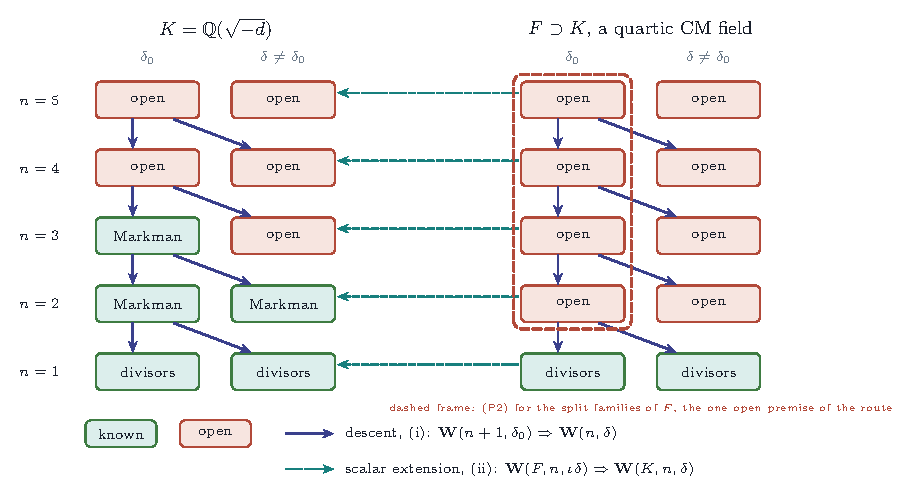
\includegraphics[width=0.94\textwidth]{fig_descent}
\caption{The Weil families of an imaginary quadratic field $K$ and of a
quartic CM field $F\supset K$, one cell for each $n$ and each kind of
discriminant, grass where the Weil classes are proved algebraic
(divisor classes at $n=1$; Markman \cite{Mar25a,Mar25b} at $n=2$ and at
$n=3$, $\delta=\delta_{0}$) and clay where they rest on the open
propagation statement. The indigo arrows
are the descent of \Cref{prop:descent}(i), from the trivial discriminant in
dimension $n+1$ to every discriminant in dimension $n$; the dashed teal
arrows are the scalar extension of \Cref{prop:descent}(ii). The dashed frame
is the propagation statement for the split families of the field of higher
degree, which by \Cref{thm:closure}(ii) is the only form of (P2) that any
minimal route to the conjecture uses: every clay cell of the left panel lies
below it.}
\label{fig:descent}
\end{figure}

\noindent
The list is as follows.

\begin{enumerate}[label=\textup{(C\arabic*)},leftmargin=3.0em,itemsep=4pt]
\item \emph{One secant object on one fourfold.} There should exist a
  principally polarised abelian fourfold $(X,\Theta)$ and a perfect complex
  $\cF$ on it with $\ch(\cF)=u_{\Theta}+3v_{\Theta}$ satisfying
  \eqref{eq:heisenberg}. By \Cref{thm:factor} and \Cref{cor:markmancondition}
  the transform $\Phi(\cF\boxtimes\cF)$ would then satisfy the weakened
  criterion, and by \Cref{prop:markman8} the three conditions of Markman's
  strategy that concern only the Chern character hold at the point $(1,3)$
  for any such $\cF$, since they depend on $\ch(\cF)$ alone. Turning this
  into algebraicity needs one further input. The weakened criterion enters
  in place of the hypothesis Markman verifies, and the survival of the
  semiregularity theorem under the substitution is exactly
  \cite[Question 11.4]{Mar25b}. So (C1) is a demand on a construction, and an affirmative answer to
  that question is a separate prerequisite standing beside it;
  \Cref{thm:closure} places both. What this paper contributes is the exact
  form of the demand. The local part of the criterion is a condition on depth
  and nothing else: if the support is Cohen--Macaulay there is no local
  obstruction at any point (\Cref{thm:cmvanishing}); if it is not, the local
  $\Ext^{2}$ is nonzero at the bad points, and where two smooth branches of
  codimension two meet transversally the criterion fails outright
  (\Cref{thm:candidatefails}, \Cref{cor:localobstruction},
  \Cref{cor:cmdichotomy}). The candidate of
  \cite[Section 12]{Mar25b} is of the second kind, and it cannot be moved to
  the first: separating the branches is what would restore the depth, and
  \Cref{rem:normalisationcm} shows that doing so moves the Chern character
  off the secant plane. What is needed is therefore a support without such
  points. For a Cohen--Macaulay support the identity \eqref{eq:heisenberg}
  is the single vanishing of the image of $A_{\theta}A_{\theta'}$ in
  $H^{1}(Z,\cE xt^{1}(\cI_{Z},\cI_{Z}))$, and the sheaf must in addition
  extend to first order along the polarised deformations
  (\Cref{thm:factor}(iii)). Such a support has one of two
  shapes (\Cref{cor:disjointroutes}): a smooth one, where the invariants are forced
  outright and $d\le b^{2}$ for the twist $b\Theta$, so $d\le9$ for the twist
  $3\Theta$ of \Cref{setup:markman} (\Cref{thm:smoothinvariants},
  \Cref{cor:fourdiscriminants}), and a singular one. In neither may the
  Hilbert--Burch resolution split into powers of $\Theta$ or into simple
  semi-homogeneous bundles (\Cref{thm:nosplit}, \Cref{thm:noblocks}), and
  no complete intersection occurs (\Cref{thm:noci}).
\item \emph{The same for every $n$ and every discriminant.} A positive answer
  to (C1) reaches one triple, and the discriminant of that triple is the
  trivial one, because the object lives on $X\times\widehat X$ and every split
  member has trivial discriminant by \Cref{prop:splitgeom}(ii). The other
  triples are reached through \Cref{prop:descent}: a positive answer in
  infinitely many dimensions gives $\mathbf{W}(K,n,\delta)$ for every $n$ and
  every $\delta$, so only uniformity in $n$ is asked for, and (C1) at $n=4$,
  with Question~11.4, already gives every sixfold. No answer of this kind
  reaches the CM fields of degree at least four. What this paper
  contributes: three of the four ingredients of \Cref{q:higher} are supplied
  for every $n$ and every $K$ (\Cref{thm:twoofthefour}), including the
  existence of the secant sheaves themselves (\Cref{thm:secantexists}); the
  fourth is isolated exactly (\Cref{rem:deformation}).
\item \emph{CM fields of degree larger than two.} For a CM field $F$ of
  degree $2m>2$ acting on an abelian variety, the Weil classes span a space of
  dimension $2m$, and the secant framework of \Cref{sec:construction}, which
  is built on a plane meeting the spinor variety in a conjugate pair, does not
  apply to them as it stands. Markman has extended it to these fields
  \cite{Mar25c}: for an abelian variety $X$ with real multiplication by the
  totally real subfield $F_{0}$ of $F$, a polarisation
  $\Theta\in\bigwedge^{2}_{F_{0}}H^{1}(X,\QQ)$ and $q\in F_{0}$ with
  $F=F_{0}(\sqrt{-q})$, he makes $F$ act on $X\times\widehat{X}$ with split
  Weil type, replaces the plane by a rational subspace $B$ of dimension
  $2^{[F_{0}:\QQ]}$ of the half-spin representation that is secant to the
  spinor variety, and shows that for sheaves $F_{1},F_{2}$ on $X$ with
  characters in $B$ the class $\kappa(E)=\ch(E)\exp(-c_{1}(E)/\rk E)$ of
  $E=\Phi(F_{1}\boxtimes F_{2}^{\vee})$ stays of Hodge type on every member
  of the family, and that where it stays algebraic all Weil classes are
  algebraic \cite[Theorem~1.1.2, Proposition~10.2.1]{Mar25c}. He exhibits
  such a pair meeting his non-degeneracy criterion when $F$ is biquadratic
  and $X$ is the Jacobian of a curve of genus four with real multiplication
  by $F_{0}$ and an automorphism acting through a unit of norm one
  \cite[Example~11.2.7, Lemma~11.2.8]{Mar25c}. That $\kappa(E)$ stays
  algebraic would follow from a semiregularity property of $E$, which is not
  addressed there \cite[Question~11.2.2]{Mar25c}; for the pair of that
  example the weaker property asked in the question fails at the points of
  the glued curves (\Cref{cor:markmanquarticfails}). No result of this paper
  depends on a theorem of \cite{Mar25c}; \Cref{ssec:quartic} and
  \Cref{ssec:sextic} use its construction as their setting. What this paper
  contributes: everything except the propagation. By \Cref{sec:cmfields}
  each such family has a connected period domain, a flat space of Weil
  classes, a dense set of rational orbits, a base point at a CM member where
  the classes are written as polynomials in divisor classes
  (\Cref{thm:cmbasepoint}), and the two propagation criteria
  (\Cref{thm:cmpropagation}); so the higher CM fields are the same
  propagation problem as the quadratic ones, and not a separate entry. For a
  quartic field at $n=2$, the smallest case of higher degree,
  \Cref{ssec:quartic}
  determines how far divisor classes, scalar extension and correspondences
  reach, and computes the number that the polarised criterion asks of one
  complex. For a sextic field, \Cref{ssec:sextic} shows that the dimension
  count, which excludes a minimal Orlov product over a quartic field, does not
  exclude one over a sextic field, and gives the profile such an object would
  have. \Cref{app:albert} places the imaginary quadratic case inside Albert's
  classification.
\item \emph{The non-split sixfolds.} $\mathbf{W}(K,3,\delta)$ for
  $\delta\ne\delta_{0}$; the case $\delta=\delta_{0}$ is Markman's
  \cite{Mar25a}. By \Cref{prop:descent}(i) it would follow from
  $\mathbf{W}(K,4,\delta_{0})$, and by \Cref{prop:descent}(ii) from
  $\mathbf{W}(K(\sqrt2),3,\iota(\delta))$. What this paper contributes: a base
  point in every family, at a member with quaternionic multiplication
  (\Cref{thm:everyfamily}); the locus of such members is a Lagrangian
  Grassmannian of codimension $n(n-1)/2$ (\Cref{prop:lagrangian}), and
  the rest of the family can be reached from it only by propagation.
\item \emph{Exceptional classes that are not of Weil type.} On an abelian
  variety the Hodge ring can contain exceptional classes that the Weil
  construction does not produce. Through dimension five it does not
  \cite{MZ99}, and in dimension eight it does: the self-product of an abelian
  fourfold of Mumford type carries two Hodge classes that are neither
  products of divisor classes nor Weil classes of any quotient
  (\Cref{prop:mumfordproduct}). So the Hodge conjecture for abelian varieties
  does not reduce to Weil classes, and the statement needed is the
  algebraicity of these classes themselves. What this paper contributes: the
  example, made exact, and the forms of their algebraicity studied in
  \Cref{sec:beyond}.
\item \emph{Varieties that are not abelian.} A reduction of the Hodge
  conjecture for arbitrary smooth projective varieties to abelian varieties
  cannot be of Hodge-theoretic kind: the $H^{3}$ of a very
  general quintic threefold lies outside the tensor category generated by the
  cohomology of abelian varieties (\Cref{prop:noabeliantype}), so its Hodge
  structure cannot be realised inside that of an abelian variety by any
  correspondence. \Cref{thm:hyperplane} and \Cref{thm:returntrip} close the
  two routes through hyperplane sections that would be the natural candidates.
  What this paper contributes: those three obstructions and, on the positive
  side, special cases only (\Cref{prop:mumfordfivefold},
  \Cref{rem:f3primefrontier}). Nor is this entry the complement of the others. The varieties
  that are not abelian include $A\times\PP^{1}$ for every abelian variety
  $A$, and the
  conjecture for $A\times\PP^{1}$ gives it for $A$, so the conjecture for
  the varieties that are not abelian is the whole conjecture
  (\Cref{prop:f3ishc}).
\end{enumerate}

\subsection{Implications from the literature}\label{ssec:bullseye}

The theorems of this paper are not the only implications that end in the
conjecture. The literature supplies others, and a frontier drawn without
them overstates what is needed. This subsection proves those implications, or
quotes them where they are theorems of the literature, so that
\Cref{ssec:closure} runs over both. Nothing in it is new
except the assembly, but the assembly changes the answer.

\begin{definition}[Three statements about all varieties]\label{def:lmv}
Here a variety is smooth, projective and defined over $\CC$, except the base
$S$ in \textup{(V)}.
\begin{enumerate}[leftmargin=3.0em,itemsep=3pt]
\item[\textup{(L)}] $B(X)$ holds for every variety $X$ (\Cref{def:Bconj}).
\item[\textup{(M)}] Every Hodge class on every variety $X$ is
  \emph{motivated} in the sense of Andr\'e \cite[\S2.1]{And96b}: it equals
  $\mathrm{pr}_{*}(\alpha\cup{*}\beta)$ for some variety $Y$, algebraic
  classes $\alpha,\beta$ on $X\times Y$, the projection
  $\mathrm{pr}\colon X\times Y\to X$, and the Lefschetz involution ${*}$ of
  $H^{*}(X\times Y,\QQ)$ with respect to some ample class.
\item[\textup{(V)}] For every smooth connected complex variety $S$, every
  smooth projective morphism $f\colon\cX\to S$ and every global section $\xi$
  of $R^{2p}f_{*}\QQ$ over $S^{\mathrm{an}}$: if $\xi_{s}$ is algebraic at one
  point $s\in S$, then $\xi_{t}$ is algebraic at every point $t\in S$.
\end{enumerate}
The Lefschetz involution of a variety $Z$ of dimension $e$ with ample class
$L$ sends $L^{r}x$, for $x$ primitive of degree $j$ and $0\le r\le e-j$, to
$\pm L^{e-j-r}x$, with a sign that depends only on $j$ \cite{And96b}; the
sign plays no role below.
\end{definition}

The statement (V) is the variational Hodge conjecture for algebraic classes;
it asks nothing about Hodge classes, only that algebraicity, once present,
survives deformation.

\begin{lemma}[Kleiman]\label{lem:lefinvolution}
Let $Z$ be a variety of dimension $e$ with ample class $L$, and suppose that
$B(Z)$ holds. Then the K\"unneth projectors $\pi_{k}$ of $H^{*}(Z,\QQ)$, the
projectors onto the summands $L^{r}P^{j}$ of the Lefschetz decomposition, and
the Lefschetz involution ${*}$ are all induced by algebraic cycles on
$Z\times Z$.
\end{lemma}

\begin{proof}
Operators induced by algebraic cycles on $Z\times Z$ are closed under sums
and rational multiples, and under composition, because the composite of two
algebraic correspondences is again algebraic \cite{Kle68}. The operator $L$
is induced by the image of a divisor of class $L$ under the diagonal, and $\Lambda$ by $B(Z)$. With
$[L,\Lambda]=H$ and $H$ acting on $H^{k}$ by $k-e$ (the proof of
\Cref{lem:LambdaL}), $H=L\Lambda-\Lambda L$ is induced by an algebraic cycle,
and since the numbers $k-e$ for $0\le k\le 2e$ are distinct,
\[
  \pi_{k}=\prod_{i\ne k}\frac{H-(i-e)}{k-i}
\]
is as well. Put $\Omega=H^{2}+2H+4\Lambda L$. For $x$ primitive of degree
$j$ put $m=e-j\ge0$. Then $\Lambda x=0$ and $Hx=-mx$, and the relation
\begin{equation}\label{eq:lambdapower}
  \Lambda L^{s}x=s(m-s+1)\,L^{s-1}x\qquad(s\ge1)
\end{equation}
follows by induction from $\Lambda L=L\Lambda-H$: the case $s=1$ is
\Cref{lem:LambdaL}, and
$\Lambda L^{s}x=L\Lambda L^{s-1}x-HL^{s-1}x
=\bigl((s-1)(m-s+2)-(2s-2-m)\bigr)L^{s-1}x=s(m-s+1)L^{s-1}x$.
So $\Omega x=(m^{2}-2m+4m)x=m(m+2)x$, and $\Omega$ commutes with $L$, since
$[L,H]=-2L$ and $[L,\Lambda L]=HL$ give $[L,\Omega]=-2(LH+HL)-4L+4HL=0$;
hence $\Omega$ acts on $L^{r}P^{j}$ by $m(m+2)$. Inside $H^{k}$ the summands
are $L^{r}P^{k-2r}$, with $m=e-k+2r$, and $m\mapsto m(m+2)$ is injective on
$m\ge0$, so Lagrange interpolation in $\Omega$ composed with $\pi_{k}$ gives
the projector $p_{k,r}$ onto $L^{r}P^{k-2r}$ as an algebraic operator.
Finally let $x\in P^{j}$ and $0\le r\le m$. If $2r\le m$, then
$L^{m-2r}(L^{r}x)=L^{m-r}x$. If $2r>m$, put $t=2r-m$, so $1\le t\le r$;
by \eqref{eq:lambdapower},
\[
  \Lambda^{t}L^{r}x=\prod_{i=0}^{t-1}(r-i)(m-r+i+1)\;L^{m-r}x,
\]
and every factor is at least $1$, because $r-i\ge r-t+1\ge1$ and
$m-r+i+1\ge m-r+1\ge1$. So on $L^{r}P^{j}$ the involution is $\pm L^{m-2r}$
or a nonzero rational multiple of $\Lambda^{2r-m}$, and
${*}=\sum_{k,r}c_{k,r}T_{k,r}\,p_{k,r}$ with rational $c_{k,r}$ and
$T_{k,r}$ a power of $L$ or of $\Lambda$. Every term is algebraic.
\end{proof}

\begin{proposition}[The conjecture is (L) and (M)]\label{prop:lefmot}
The Hodge conjecture for every variety is equivalent to \textup{(L)} and
\textup{(M)} together.
\end{proposition}

\begin{proof}
Assume the conjecture. Then \textup{(L)} holds by \Cref{thm:equivalence}. An
algebraic class $\xi$ on $X$ of dimension $d$ is motivated: take $Y$ a point,
$\alpha=\xi$, and $\beta=\varepsilon h^{d}$ with $h$ the ample class and
$\varepsilon=\pm1$ the sign for which ${*}(h^{d})=\varepsilon$, which exists
because the unit $1\in H^{0}$ is primitive of degree $0$; then
$\alpha\cup{*}\beta=\xi$. Every Hodge class is algebraic, so \textup{(M)}
holds.

Conversely assume \textup{(L)} and \textup{(M)}, and let $\xi$ be a Hodge
class on $X$. By \textup{(M)}, $\xi=\mathrm{pr}_{*}(\alpha\cup{*}\beta)$ with
$\alpha,\beta$ algebraic on $X\times Y$. By \textup{(L)}, $B(X\times Y)$
holds, so ${*}$ is induced by an algebraic cycle
(\Cref{lem:lefinvolution}); hence ${*}\beta$, the product
$\alpha\cup{*}\beta$ and its push-forward $\xi$ are algebraic. This is
Andr\'e's observation that motivated classes are algebraic as soon as the
Lefschetz involutions are \cite[\S2.1]{And96b}.
\end{proof}

\begin{proposition}[Two sources of (V)]\label{prop:lefvhc}
The Hodge conjecture implies \textup{(V)}, and so does \textup{(L)}.
\end{proposition}

\begin{proof}
Let $f\colon\cX\to S$, $\xi$ and $s$ be as in \textup{(V)}, with $\xi_{s}$
algebraic. As $S$ is smooth and connected it is irreducible, so two affine
open subsets meet, and it suffices to treat $S$ affine, joining $s$ to an
arbitrary $t$ through a point of the intersection of an affine neighbourhood
of each. Then $\cX$ is quasi-projective and, by resolution of singularities,
has a smooth projective compactification $\overline{\cX}$.

Assume the conjecture. Write $n=2p$ and
$\rho\colon H^{n}(\overline{\cX},\QQ)\to H^{0}(S^{\mathrm{an}},R^{n}f_{*}\QQ)$
for restriction; it is surjective by the theorem of the fixed part
\cite[4.1.1(ii)]{Del71}. For $t\in S$ the restriction
$r_{t}\colon H^{n}(\overline{\cX},\QQ)\to H^{n}(\cX_{t},\QQ)$ is $\rho$
followed by evaluation at $t$, and evaluation is injective because $S$ is
connected; so $K=\ker r_{t}=\ker\rho$ does not depend on $t$. It is a
sub-Hodge structure, and the Hodge structure $H^{n}(\overline{\cX},\QQ)$ is
polarisable, hence semisimple, so $H^{n}(\overline{\cX},\QQ)=K\oplus K'$
with $K'$ a sub-Hodge structure. Choose $\eta\in K'$ with $\rho(\eta)=\xi$.
Then $r_{s}|_{K'}$ is an injective morphism of Hodge structures and
$r_{s}(\eta)=\xi_{s}$ is of type $(p,p)$, so every component of $\eta$ of
type other than $(p,p)$ maps to zero and is zero: $\eta$ is a Hodge class.
So $\xi_{t}=r_{t}(\eta)$ is a Hodge class on $\cX_{t}$ for every $t$, and
algebraic by the conjecture.

Assume \textup{(L)}. The algebraic class $\xi_{s}$ is motivated (proof of
\Cref{prop:lefmot}), so $\xi_{t}$ is motivated for every $t$ by Andr\'e's
deformation theorem \cite[Th\'eor\`eme~0.5]{And96b}, and a motivated class is
algebraic under \textup{(L)} (proof of \Cref{prop:lefmot}).
\end{proof}

\begin{theorem}[Deligne, Andr\'e; Abdulali, Andr\'e]\label{thm:vhcab}
\textup{(V)} implies the Hodge conjecture for every abelian variety, and so
does \textup{(L)}.
\end{theorem}

\begin{proof}
Milne calls a class \emph{accessible} if it lies in the least family of
rational classes that contains the classes of algebraic cycles, is stable
under pull-back by morphisms of varieties, and contains $t_{t}$ for every $t$
whenever $(t_{s})_{s\in S}$ is a global section of $R^{r}f_{*}\QQ$ for a
smooth projective family over a smooth connected base and contains $t_{s}$
for one $s$; and he proves, following Deligne and Andr\'e, that every Hodge
class on an abelian variety is accessible \cite[\S5.1, Theorem~3]{Mil20}.
The algebraic classes contain the classes of algebraic cycles and are stable
under pull-back, and under \textup{(V)} they have the third property. So they
contain every accessible class, hence every Hodge class on an abelian
variety; this is \cite[Remark~2]{Mil20}. The statement for \textup{(L)}
follows by \Cref{prop:lefvhc}, and is the theorem of Abdulali and Andr\'e in
the form of \cite[Theorem~4]{Mil20}.
\end{proof}

\begin{remark}[The three in the literature]\label{rem:lmvknown}
$B(X)$ is known for curves, where it is immediate,
and for abelian varieties \cite[\S2]{Kle68}, and \Cref{cor:mumfordlefschetz}
below adds the total space of every Mumford family. \textup{(M)} holds for the Hodge
classes on abelian varieties \cite[Th\'eor\`eme~0.6.2]{And96b}.
\textup{(V)} holds in degree $2$, where by the argument of
\Cref{prop:lefvhc} the class $\xi_{t}$ is a Hodge class and the Lefschetz
theorem on $(1,1)$ classes applies; the one general mechanism for it in
higher degree is the semiregularity theorem \cite{Blo72,BF03,Pri24}, which is the
mechanism of \Cref{thm:semiregclosure}. \Cref{thm:vhcab} says what is at
stake for this paper: the single statement \textup{(V)}, which the conjecture
itself implies, gives the Weil classes of every CM field and the classes
beyond the Weil lines at once, by a route that uses none of the theorems
proved here.
\end{remark}

\subsection{The Lefschetz standard conjecture for abelian schemes over curves}
\label{ssec:newlefschetz}

The statement $B(X)$ is known for abelian varieties $X$. This subsection
proves it for the total space
of an abelian scheme over a curve whose invariant cycles are algebraic, and
so for the total space of every Mumford family. The proof assembles the
operator $\Lambda$ from a relative part, which is a Pontryagin product and is
algebraic on every abelian scheme, and a part along the base, which is
algebraic exactly when the invariant cycles are.

\begin{proposition}[$\Lambda$ as a Pontryagin product]
\label{prop:pontryaginlambda}
Let $A$ be an abelian variety of dimension $g$, $\ell\in H^{2}(A,\QQ)$ the
class of an ample line bundle, $D=\int_{A}\ell^{g}/g!$ and
$\gamma=\ell^{g-1}/(g-1)!$. Let $\mu\colon A\times A\to A$ be the addition
and $x\star y=\mu_{*}(p_{1}^{*}x\cup p_{2}^{*}y)$ the Pontryagin product.
Then the operator $\Lambda$ of \Cref{def:Bconj} for the class $\ell$ is
\[
  \Lambda(x)=D^{-1}\,x\star\gamma .
\]
In particular $\Lambda$ is induced by the algebraic cycle
$D^{-1}(p_{1},\mu)_{*}(p_{2}^{*}Z)$ on $A\times A$, for any cycle $Z$ of
class $\gamma$.
\end{proposition}

\begin{proof}
Put $V=H_{1}(A,\QQ)$, so that $H^{*}(A,\QQ)=\bigwedge^{*}V^{\vee}$ under cup
product and $H_{*}(A,\QQ)=\bigwedge^{*}V$ under the Pontryagin product of
homology, and let $\mathrm{PD}(x)=x\cap[A]$. Cap product makes
$H_{*}$ a module over $H^{*}$, and for a torus it is contraction; so
$\mathrm{PD}(\ell\cup x)=\ell\cap\mathrm{PD}(x)$ is the contraction
$\iota_{\ell}$ applied to $\mathrm{PD}(x)$. Poincar\'e duality commutes
with $\mu_{*}$ and carries $p_{1}^{*}x\cup p_{2}^{*}y$ to the cross product
of $\mathrm{PD}(x)$ and $\mathrm{PD}(y)$, without sign when $y$ has even
degree, so $\mathrm{PD}(x\star\gamma)=\mathrm{PD}(x)\cdot\beta$ with
$\beta=\mathrm{PD}(\gamma)\in\bigwedge^{2}V$.

Choose a basis $x_{1},y_{1},\dots,x_{g},y_{g}$ of $V^{\vee}$ with
$\ell=\sum_{i}d_{i}\,x_{i}\wedge y_{i}$, $d_{i}>0$, oriented so that
$\int_{A}x_{1}\wedge y_{1}\wedge\dots\wedge x_{g}\wedge y_{g}=1$; then
$\int_{A}\ell^{g}=g!\,d_{1}\cdots d_{g}$, so $D=d_{1}\cdots d_{g}$. Let
$e_{i},f_{i}$ be the dual basis of $V$. Then
$\gamma=\sum_{j}\bigl(\prod_{i\ne j}d_{i}\bigr)\prod_{i\ne j}x_{i}\wedge y_{i}$
and $\beta=\varepsilon D\sum_{j}d_{j}^{-1}e_{j}\wedge f_{j}$ with
$\varepsilon=\pm1$ independent of $j$, since the permutations of the pairs
preserve the orientation and exchange the terms. The algebra $\bigwedge^{*}V$
is the graded tensor product of the algebras
$\bigwedge^{*}\langle e_{i},f_{i}\rangle$, and $\iota_{\ell}$ and
multiplication by $D^{-1}\beta$ are sums over $i$ of even operators on the
$i$-th factor, namely $d_{i}\,\iota_{x_{i}\wedge y_{i}}$ and
$\varepsilon d_{i}^{-1}e_{i}\wedge f_{i}$. Operators on different factors
commute, and on the $i$-th factor, with basis $1,e_{i},f_{i},e_{i}\wedge
f_{i}$ and $\iota_{x_{i}\wedge y_{i}}(e_{i}\wedge f_{i})=\sigma$ for a sign
$\sigma$ fixed by the convention for contraction, the commutator
$[\iota_{\ell},D^{-1}\beta]$ acts by $\varepsilon\sigma$ on $1$, by $0$ on
$e_{i}$ and $f_{i}$, and by $-\varepsilon\sigma$ on $e_{i}\wedge f_{i}$, that
is by $\varepsilon\sigma(1-k_{i})$ in degree $k_{i}$. Summing over $i$,
$[\iota_{\ell},D^{-1}\beta]=\varepsilon\sigma(g-k)$ on $\bigwedge^{k}V$. As
$\mathrm{PD}$ carries $H^{q}$ to $\bigwedge^{2g-q}V$, the operator
$\Lambda'(x)=D^{-1}x\star\gamma$ satisfies
$[L,\Lambda']=\varepsilon\sigma(q-g)=\varepsilon\sigma H$ on $H^{q}(A)$.

The sign is fixed by one value. For $x$ and $y$ of complementary degrees,
$x\star y\in H^{0}(A)$ is $\int_{A\times A}p_{1}^{*}x\cup p_{2}^{*}y\cup
\mu^{*}[\mathrm{pt}]$, and $\mu^{*}[\mathrm{pt}]$ is the class of the
antidiagonal $\{(a,-a)\}$, so $x\star y=\int_{A}x\cup[-1]^{*}y$; for
$y=\gamma$, of even degree, this is $\int_{A}x\cup\gamma$. Hence
$\Lambda'(\ell)=D^{-1}\int_{A}\ell\cup\gamma=g$, while
$\Lambda(\ell)=\Lambda(L\cdot1)=g$ by \Cref{lem:LambdaL}. If
$\varepsilon\sigma=-1$, then $-\Lambda'$ would be the operator of
\Cref{def:Bconj} and $\Lambda'(\ell)=-g$. So $\varepsilon\sigma=1$, and
$\Lambda'=\Lambda$ by the uniqueness in \Cref{def:Bconj}. Finally, the
correspondence $(p_{1},\mu)_{*}(p_{2}^{*}Z)$ acts by
$x\mapsto p_{2*}\bigl(p_{1}^{*}x\cup(p_{1},\mu)_{*}p_{2}^{*}[Z]\bigr)
=\mu_{*}(p_{1}^{*}x\cup p_{2}^{*}\gamma)$, by the projection formula.
\end{proof}

\begin{theorem}[The Lefschetz operator of an abelian scheme over a curve;
cf.\ Tankeev \cite{Tan03}]
\label{thm:lefschetzfamily}
Let $C$ be a smooth projective connected curve and $\pi\colon W\to C$ an
abelian scheme of relative dimension $g$ with $W$ projective. Suppose that
every class in $H^{*}(W_{c},\QQ)$ invariant under the monodromy of
$R^{*}\pi_{*}\QQ$ is the restriction of an algebraic class on $W$. Then there
is an ample class $L_{W}$ on $W$ whose operator $\Lambda$ is induced by an
algebraic cycle on $W\times W$: $B(W)$ holds.
\end{theorem}

\begin{proof}
\emph{Step 1: the decomposition.} Let $[n]\colon W\to W$ be multiplication
by $n$ over $C$. It acts on $R^{q}\pi_{*}\QQ=\bigwedge^{q}R^{1}\pi_{*}\QQ$ by
$n^{q}$. The Leray spectral sequence degenerates \cite[4.1.1(i)]{Del71}, and
$[2]^{*}$ preserves the Leray filtration and acts on its graded pieces
$H^{p}(C,R^{q}\pi_{*}\QQ)$ by $2^{q}$. So $H^{k}(W,\QQ)=\bigoplus_{q}
H^{k}_{(q)}$, where $H^{k}_{(q)}$ is the $2^{q}$-eigenspace of $[2]^{*}$ and
maps isomorphically onto $H^{k-q}(C,R^{q}\pi_{*}\QQ)$; only $k-q\in\{0,1,2\}$
occurs. The projectors
$P_{q}=\prod_{q'\ne q}([2]^{*}-2^{q'})/(2^{q}-2^{q'})$ are induced by
algebraic cycles, polynomials in the graph of $[2]$. As $[2]^{*}$ is a ring
homomorphism, $H_{(q)}\cup H_{(q')}\subset H_{(q+q')}$; as
$\int_{W}[2]^{*}z=2^{2g}\int_{W}z$, the integral vanishes on $H_{(q)}$ for
$q\ne2g$, so Poincar\'e duality pairs $H_{(q)}$ with $H_{(2g-q)}$ only; and
$[2]_{*}=2^{2g}([2]^{*})^{-1}$ acts on $H_{(q)}$ by $2^{2g-q}$.

\emph{Step 2: the ample class.} Let $\cL$ be a relatively ample line bundle,
replaced by $\cL\otimes[-1]^{*}\cL$ so that it is symmetric. Then $[-1]^{*}$
fixes $c_{1}(\cL)$ and acts on $H_{(q)}$ by $(-1)^{q}$, so $c_{1}(\cL)$ has no
component in $H^{2}_{(1)}$, while $H^{2}_{(0)}=H^{2}(C,\QQ)$ is spanned by the
class $f$ of a fibre. So $c_{1}(\cL)=\ell+af$ with $\ell\in H^{2}_{(2)}$
algebraic and $a\in\QQ$. Put $L_{W}=\ell+mf=c_{1}(\cL)+(m-a)f$ with
$m\in\QQ$ so large that $L_{W}$ is a positive rational multiple of the class
of an ample line bundle, which is possible because $\cL$ is relatively ample.
Write $L_{\mathrm{rel}}$ and $L_{C}$ for cup product with $\ell$ and with
$mf$, so that $L_{W}=L_{\mathrm{rel}}+L_{C}$; on
$H^{p}(C,R^{q}\pi_{*}\QQ)$ the first raises $q$ by two and the second raises
$p$ by two.

\emph{Step 3: the relative operator.} Put $\gamma=\ell^{g-1}/(g-1)!$, which is
algebraic and lies in $H_{(2g-2)}$, and $D=\int_{W_{c}}\ell^{g}/g!$. Let
$\mu,\mathrm{pr}_{1},\mathrm{pr}_{2}\colon W\times_{C}W\to W$ be the addition
and the projections, and $T(x)=\mu_{*}(\mathrm{pr}_{1}^{*}x\cup
\mathrm{pr}_{2}^{*}\gamma)$. As in \Cref{prop:pontryaginlambda}, $T$ is
induced by the algebraic cycle $(\mathrm{pr}_{1},\mu)_{*}(\mathrm{pr}_{2}^{*}Z)$
on $W\times W$. Since $\pi\circ\mathrm{pr}_{1}=\pi\circ\mu$, the projection
formula gives $T(x\cup\pi^{*}b)=T(x)\cup\pi^{*}b$, so $T$ commutes with
$L_{C}$. Since $[2]\circ\mu=\mu\circ([2]\times_{C}[2])$,
$[2]_{*}T(x)=\mu_{*}(\mathrm{pr}_{1}^{*}[2]_{*}x\cup\mathrm{pr}_{2}^{*}
[2]_{*}\gamma)$, and for $x\in H_{(q)}$ this is
$2^{2g-q}\,2^{2}\,T(x)$; so $T$ maps $H_{(q)}$ into $H_{(q-2)}$. A relative
correspondence acts on the Leray spectral sequence through the maps it
induces on the local systems, so on $H^{p}(C,R^{q}\pi_{*}\QQ)$ the operator
$T$ is $H^{p}(C,T_{\bullet})$, with $T_{c}$ the Pontryagin product with
$\gamma|_{W_{c}}$ on the fibre. By \Cref{prop:pontryaginlambda}, $D^{-1}T_{c}$
is the operator $\Lambda$ of the fibre, so $\Lambda_{\mathrm{rel}}=D^{-1}T$
satisfies $[L_{\mathrm{rel}},\Lambda_{\mathrm{rel}}]=H_{\mathrm{rel}}$, where
$H_{\mathrm{rel}}$ acts on $H_{(q)}$ by $q-g$.

\emph{Step 4: the invariant classes.} Restriction maps $H^{q}(W,\QQ)$ onto the
monodromy invariants $I_{q}\subset H^{q}(W_{c},\QQ)$ \cite[4.1.1(ii)]{Del71},
and it kills $H^{q}_{(q')}$ for $q'<q$, which lies in positive Leray degree;
so it maps $H^{q}_{(q)}$ isomorphically onto $I_{q}$. Every element of
$H^{q}_{(q)}$ is algebraic: if $v\in I_{q}$ is the restriction of an algebraic
class $z$, then $P_{q}z$ is algebraic, lies in $H^{q}_{(q)}$ and restricts to
$v$. The subspace $I_{q}$ is a sub-Hodge structure, as the image of a
morphism of Hodge structures, and it is stable under cup product with
$\ell_{c}$ and under the operator $\Lambda$ of the fibre, which are the
restrictions of $L_{\mathrm{rel}}$ and $\Lambda_{\mathrm{rel}}$. The
polarisation of $H^{q}(W_{c},\QQ)$ attached to $\ell_{c}$ has the form
$(v,w)\mapsto\int_{W_{c}}v\cup S(w)$, with $S$ a polynomial in cup product
with $\ell_{c}$, the operator $\Lambda$ and the projectors of the fibre, and
its restriction to the sub-Hodge structure $I_{q}$ is again a polarisation
\cite{Voi02}. Since $S(I_{q})\subset I_{2g-q}$, the pairing
$I_{q}\times I_{2g-q}\to\QQ$ is nondegenerate.

\emph{Step 5: the operator along the base.} For $y\in H^{q}_{(q)}$ and
$w\in H^{2g-q}_{(2g-q)}$ one has $\int_{W}(y\cup f)\cup w=\int_{W_{c}}
y|_{W_{c}}\cup w|_{W_{c}}$. By Step 4 and Step 1 this shows that
$L_{C}\colon H^{q}_{(q)}\to H^{q+2}_{(q)}$ is injective, and it is onto
because $\dim H^{q+2}_{(q)}=\dim H^{2g-q}_{(2g-q)}=\dim I_{2g-q}=\dim I_{q}$,
by Poincar\'e duality on $W$ and on the invariants. Choose bases $(a_{j})$ of
$H^{q}_{(q)}$ and $(b_{k})$ of $H^{2g-q}_{(2g-q)}$, all algebraic by Step 4,
let $M_{jk}=\int_{W}a_{j}\cup mf\cup b_{k}$, which is invertible, and put
\[
  \Lambda_{C}(x)=\sum_{j,k}(M^{-1})_{kj}\Bigl(\int_{W}x\cup b_{k}\Bigr)a_{j}
  \qquad(x\in H^{q+2}(W,\QQ)),
\]
for every $q$. It is induced by the algebraic cycle
$\sum_{j,k}(M^{-1})_{kj}\,b_{k}\times a_{j}$. By Step 1, $\int_{W}x\cup b_{k}$
vanishes for $x\in H^{q+2}_{(q')}$ with $q'\ne q$, so $\Lambda_{C}$ is zero
on $H^{p}(C,R^{q}\pi_{*}\QQ)$ for $p\ne2$, and $\Lambda_{C}(L_{C}a_{i})=a_{i}$.
Hence $[L_{C},\Lambda_{C}]$ is $-1$ on $H_{(q)}^{q}$, $0$ on
$H_{(q)}^{q+1}$ and $+1$ on $H_{(q)}^{q+2}$: it is the operator $H_{C}$ that
acts on $H^{p}(C,R^{q}\pi_{*}\QQ)$ by $p-1$.

\emph{Step 6: the cross relations and the conclusion.} $[L_{C},
\Lambda_{\mathrm{rel}}]=0$ by Step 3. Both $L_{\mathrm{rel}}\Lambda_{C}$ and
$\Lambda_{C}L_{\mathrm{rel}}$ vanish off the summands with $p=2$, and on
$L_{C}y$ with $y\in H^{q}_{(q)}$ both give $\ell\cup y$, because
$\ell\cup y\in H^{q+2}_{(q+2)}$ and $L_{C}$ commutes with $L_{\mathrm{rel}}$;
so $[L_{\mathrm{rel}},\Lambda_{C}]=0$. Put
$\Lambda=\Lambda_{\mathrm{rel}}+\Lambda_{C}$, of degree $-2$. Then
\[
  [L_{W},\Lambda]=[L_{\mathrm{rel}},\Lambda_{\mathrm{rel}}]+[L_{C},\Lambda_{C}]
  =H_{\mathrm{rel}}+H_{C},
\]
which acts on $H^{p}(C,R^{q}\pi_{*}\QQ)\subset H^{p+q}(W)$ by
$(q-g)+(p-1)=(p+q)-\dim W$. So $\Lambda$ is the operator of \Cref{def:Bconj}
for $L_{W}$, by its uniqueness, and it is induced by an algebraic cycle by
Steps 3 and 5.
\end{proof}

\Cref{fig:lefschetzgrid} draws the summands of the proof in relative
dimension four.

\begin{corollary}[Mumford families]\label{cor:mumfordlefschetz}
Let $\pi\colon W\to C$ be a non-isotrivial abelian scheme of relative dimension
four over a smooth projective connected curve, $W$ projective, whose very
general fibre $X$ is a fourfold as in \Cref{prop:mumfordproduct}, with Hodge
group the group $G$ of Mumford's construction \cite{Mum69}, the restriction of
scalars from a totally real cubic field $F$ of the norm one group of a
quaternion algebra over $F$. Then $B(W)$ holds. Such families exist, over the
compact Shimura curves of \cite{Mum69}.
\end{corollary}

\begin{proof}
By Andr\'e's theorem \cite[Theorem~1]{And92} the connected monodromy group is
a normal subgroup of the derived Mumford--Tate group of $X$, which is $G$. It
is not trivial, because the family is not isotrivial, and $G$ is $\QQ$-simple,
since over $\overline{\QQ}$ its three factors are indexed by the embeddings of
$F$ and permuted transitively by the Galois group; so it is $G$. The
monodromy invariants in $H^{*}(X,\QQ)$ are therefore contained in the
invariants of $G$, which are the Hodge classes of $X$, and these are the
powers of the polarisation by \Cref{prop:mumfordproduct}(i). The powers
of $\ell$ restrict to the powers of the polarisation, so every invariant class
is the restriction of an algebraic class, and \Cref{thm:lefschetzfamily}
applies.
\end{proof}

\begin{figure}[tbp]
\centering
  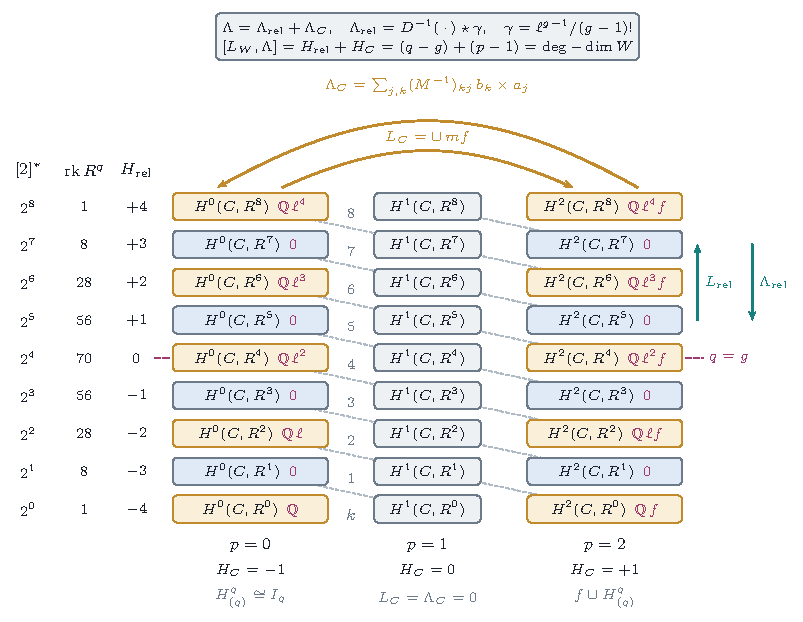
\includegraphics[width=0.86\textwidth]{fig_lefschetzgrid}
\caption{The proof of \Cref{thm:lefschetzfamily} for relative dimension
four. The boxes are the summands $H^{p}(C,R^{q}\pi_{*}\QQ)$ of $H^{*}(W,\QQ)$,
split off by the eigenvalue $2^{q}$ of $[2]^{*}$ shown on the left; the dotted
diagonals join the summands of one $H^{k}(W,\QQ)$, $k=p+q$, and the dashed
magenta line is the axis $q=g$ of hard Lefschetz on the fibres. The relative
operators $L_{\mathrm{rel}}$ and $\Lambda_{\mathrm{rel}}$, in teal, move
within a column; $\Lambda_{\mathrm{rel}}$ is a Pontryagin product with an
algebraic class on every abelian scheme (\Cref{prop:pontryaginlambda}). The
base operators $L_{C}$ and $\Lambda_{C}$, in ochre, move along a row between
the outer columns and kill the middle one; $\Lambda_{C}$ is the displayed
cycle built from bases $(a_{j})$, $(b_{k})$ of the invariant summands, and is
algebraic exactly when the invariant cycles are. Below each column is the
weight of $H=[L_{W},\Lambda]$ on it, and the panel at the top is Step 6 of the
proof. The ochre boxes carry the invariant cycles and their images under
$L_{C}$; for a Mumford family they are the lines listed in magenta on the
right, spanned by $\ell^{i}f$ (and by $\ell^{i}$ in the left column), and the
other boxes of the outer columns are zero (\Cref{cor:mumfordlefschetz}).}
\label{fig:lefschetzgrid}
\end{figure}

\begin{remark}[Scope of the argument]\label{rem:newlefschetzscope}
The total space $W$ is a fivefold fibred in abelian fourfolds whose Hodge
groups are not defined by endomorphisms; it is not a product and not an
abelian variety. For abelian schemes over curves the mechanism of
\Cref{thm:lefschetzfamily} goes back to Tankeev \cite{Tan03}, who proves $B$
for the total space when certain canonically defined Hodge cycles are
algebraic; the argument here does not use his hypotheses, and we make no
claim of priority for \Cref{cor:mumfordlefschetz}. The difficulty lies in the hypothesis of
\Cref{thm:lefschetzfamily}.
Applied to the fibre square $W\times_{C}W\to C$ the theorem gives
$B(W\times_{C}W)$ as soon as every invariant class of $X\times X$ is the
restriction of an algebraic class on $W\times_{C}W$; the invariant classes
include the two exceptional classes of \Cref{prop:mumfordproduct}, so this
is the smallest case of (F2) in a global form. \Cref{thm:lefschetzfamily} does not bear on (P2), on the Kuga--Satake
class of \Cref{thm:mumfordks}, or on \textup{(L)} for varieties that are not
fibred in abelian varieties over a curve.
\end{remark}

\begin{proposition}[Powers of a Weil variety; cf.\ \cite{Mil22}]\label{prop:powers}
Let $X$ be of $(K,-1,n)$-Weil type with $n\ge2$ and $\Hg(X)=\SU(V,H)$. For
every $k\ge1$ the $\QQ$-algebra $\Hdg^{*}(X^{k})$ is generated by the divisor
classes of $X^{k}$ and the pull-backs $f_{a}^{*}\omega$ of the Weil classes
$\omega$ of $X$ along the homomorphisms $f_{a}=\sum_{j}a_{j}\,pr_{j}\colon
X^{k}\to X$, $a\in\ZZ^{k}$. Consequently, if the Weil classes of $X$ are
algebraic, the Hodge conjecture holds for every power of $X$. By
\cite{Mar25a} this is so for every such $X$ with $n=2$, and with $n=3$ and
trivial discriminant.
\end{proposition}

\begin{proof}
Write $H^{1}(X,\CC)=V_{+}\oplus V_{-}$ for the eigenspaces of $K$ and
$W=V_{+}$. The polarisation makes $V_{+}$ and $V_{-}$ isotropic and pairs them
perfectly, so $V_{-}=W^{\vee}$, and restriction to $V_{+}$ identifies
$\SU(V,H)_{\CC}$ with $\SL(W)$. As $\Hg(X^{k})$ is $\Hg(X)$ acting diagonally
on $H^{1}(X^{k},\CC)=(W\otimes U)\oplus(W^{\vee}\otimes U)$, $U=\CC^{k}$, the
Hodge classes of $X^{k}$, tensored with $\CC$, are the $\SL(W)$-invariants in
$\bigwedge^{*}\bigl((W\otimes U)\oplus(W^{\vee}\otimes U)\bigr)$. That algebra
is an $\SL(W)$-equivariant quotient of a tensor algebra, with an equivariant
section given by antisymmetrisation, so Weyl's first fundamental theorem for
$\SL(W)$, in its tensor form and applied before antisymmetrisation, shows
that its invariants are generated by the images of the contractions and the
determinant tensors: the classes
$D(u,u')=\sum_{i}(e_{i}\otimes u)\wedge(e_{i}^{\vee}\otimes u')$ and the
polarised determinants, which by polarisation are combinations of
$\det_{u}=\bigwedge_{i}(e_{i}\otimes u)$ and
$\det^{\vee}_{u}=\bigwedge_{i}(e_{i}^{\vee}\otimes u)$, $u,u'\in U$. For
$2n\ge3$ the $D(u,u')$ span the invariants of degree two, which are the
divisor classes tensored with $\CC$. With $\alpha_{\pm}$ spanning
$\bigwedge^{2n}V_{\pm}$ (\Cref{prop:weilline}) one has
$f_{a}^{*}\alpha_{+}=\det_{a}$ and $f_{a}^{*}\alpha_{-}=\det^{\vee}_{a}$, and
since $u\mapsto\det_{u}$ is polynomial and $\ZZ^{k}$ is Zariski dense in
$U$, these span the same space as all $\det_{u}$. So the $\QQ$-algebra
generated by $\NS(X^{k})_{\QQ}$ and the $f_{a}^{*}\omega$ is contained in
$\Hdg^{*}(X^{k})$ and has the same complexification. The generators are
algebraic when the Weil classes of $X$ are, and they are for $n=2$ and for
$n=3$ at trivial discriminant by \cite{Mar25a}.
\end{proof}

The statement for powers is known (compare \cite{Mil22}, and \cite{Li26}
for the powers of CM fourfolds); we include the short proof because the next
corollary uses it.

\begin{corollary}[Abelian schemes of small relative dimension]
\label{cor:lefschetzsmall}
Let $\pi\colon W\to C$ be an abelian scheme of relative dimension $g$ over a
smooth projective connected curve, with $W$ projective, and suppose that
every monodromy invariant class in $H^{*}(W_{c},\QQ)$ is a Hodge class, as
happens when the identity component of the Zariski closure of the monodromy
group is the Hodge group of a very general fibre.
\begin{enumerate}[label=\textup{(\roman*)},leftmargin=2.6em,itemsep=2pt]
\item If $g\le4$, then $B(W)$ holds.
\item If the fibres are of $(K,-1,n)$-Weil type with connected monodromy
  group $\SU(V,H)$, and $n=2$, or $n=3$ with trivial discriminant, then
  $B$ holds for every fibre power $W\times_{C}\dots\times_{C}W$. In
  particular $B(W_{C})$ of \Cref{cor:weilequiv} holds in these cases.
\end{enumerate}
\end{corollary}

\begin{proof}
By the theorem of the fixed part the invariant classes form a sub-Hodge
structure of every fibre, with a Hodge structure independent of the point, so
they are Hodge classes on every fibre.

(i) The Hodge conjecture holds for abelian varieties of dimension at most
four, by the Lefschetz theorem on $(1,1)$ classes and hard Lefschetz up to
dimension three and by \cite{Mar25a} in dimension four, so each invariant
class is algebraic on every fibre; \Cref{lem:spreading} makes it the
restriction of an algebraic class on $W$, and \Cref{thm:lefschetzfamily}
applies.

(ii) The fibre power is an abelian scheme with projective total space and
the monodromy acting diagonally. Its invariant classes are
$\SU(V,H)$-invariants, hence Hodge classes at every member with
$\Hg=\SU(V,H)$, an uncountable set of points, and there the Hodge conjecture
holds for the fibre by \Cref{prop:powers}; \Cref{lem:spreading} and
\Cref{thm:lefschetzfamily} conclude as before. For $W_{C}$ the connected
monodromy group is $\SU(V,H)$ when it is Zariski dense, which is the
hypothesis of \Cref{cor:weilequiv}(ii).
\end{proof}

The hypothesis on the monodromy in \Cref{cor:lefschetzsmall} can be checked
with Andr\'e's theorem \cite[Theorem~1]{And92}: the identity component of the
Zariski closure of the monodromy group is always a normal subgroup of the
derived Mumford--Tate group of a very general fibre, so the hypothesis holds
whenever the family is not isotrivial and the Hodge group of a very general
fibre is semisimple and $\QQ$-simple, as for the Mumford families of
\Cref{cor:mumfordlefschetz}.

\begin{proposition}[The total space of a Mumford family]
\label{prop:mumfordfivefold}
Let $W\to C$ be as in \Cref{cor:mumfordlefschetz}, with $C$ the compact
Shimura curve of \cite{Mum69} of torsion-free level, or a finite \'etale cover
of it. Then the Hodge conjecture holds for the fivefold $W$: its Hodge classes
of degree $2p$ are spanned by $\ell^{p}$ and $f\ell^{p-1}$, with $f$ the class
of a fibre.
\end{proposition}

\begin{proof}
By Step 1 of the proof of \Cref{thm:lefschetzfamily},
$H^{k}(W,\QQ)=\bigoplus_{q}H^{k}_{(q)}$ with $H^{k}_{(q)}\cong
H^{k-q}(C,R^{q}\pi_{*}\QQ)$, the summands being sub-Hodge structures cut out by
algebraic projectors. The summand with $k=q$ is the space of invariants, which
by the proof of \Cref{cor:mumfordlefschetz} is spanned by the powers of the
polarisation, restrictions of the powers of $\ell$. The summand with $k=q+2$
is $f\cup H^{q}_{(q)}$ by Step 5, spanned by the $f\ell^{q/2}$. It remains to
see that $H^{1}(C,R^{q}\pi_{*}\QQ)$ carries no Hodge class. For $q$ even its
weight $q+1$ is odd. For $q$ odd, over $\CC$ the local system splits as a sum
of $S^{k_{1}}V_{1}\otimes U_{\lambda}\otimes M_{\lambda}$, where $V_{1}$ is the
uniformising variation of the factor of $G$ split at the real place, $U_{\lambda}$ is
a unitary variation of type $(0,0)$, $M_{\lambda}$ is constant of type $(a,a)$
with $2a+k_{1}=q$, and $k_{1}\equiv q\pmod2$ because the central element
$(-1,1,1)$ acts on $V$ by $-1$. When $C$ is \'etale over the Shimura curve the
Kodaira--Spencer map of $V_{1}$ is an isomorphism, and then
$H^{1}(C,S^{k_{1}}V_{1}\otimes U_{\lambda})$ has only the types $(k_{1}+1,0)$
and $(0,k_{1}+1)$ \cite{Zuc79}; after the twist by $M_{\lambda}$ these are
never balanced, since $k_{1}\ge1$.
\end{proof}

Statements of the kind of \Cref{prop:mumfordfivefold} are studied for Kuga
fibre varieties, and we make no claim of priority.
The \'etale hypothesis is used only at the end of the proof, and it cannot be
dropped from the argument: over a ramified cover the Kodaira--Spencer map of
$V_{1}$ vanishes at the branch points, the Higgs field of $S^{k_{1}}V_{1}$ is
no longer an isomorphism, and the torsion of its cokernel contributes to
$H^{1}(C,R^{q}\pi_{*}\QQ)$ in balanced types.

\subsection{The two targets as cases of (L)}
\label{ssec:targets}

The argument of \Cref{ssec:newlefschetz} does more than add a case of
\textup{(L)}. For an abelian scheme over a curve it shows that \textup{(L)}
for the total space is exactly the statement that algebraicity propagates
along the curve. The base points of this paper then turn each of the two
targets of \Cref{rem:bullseye}, one Weil family and the first
classes beyond the Weil lines, into \textup{(L)} for one explicit variety. The
reductions are equivalences, so they locate the difficulty rather than remove
it. Along the way the Hodge conjecture is proved for the self-product of a
Mumford fourfold at every CM point (\Cref{thm:mumfordcm}), and the two
branches of \Cref{rem:twobranches} are shown not to be realisable by two
objects (\Cref{thm:nosum}), an implication whose hypothesis
\Cref{thm:p2false} shows is never met.

\begin{lemma}[Spreading along a curve]\label{lem:spreading}
Let $\pi\colon W\to C$ be a smooth projective morphism onto a smooth projective
connected curve, $W$ projective, and $\xi$ a global section of
$R^{2p}\pi_{*}\QQ$. If $\xi_{t}$ is algebraic for uncountably many $t\in C$,
there are an algebraic class $\tilde\xi$ on $W$ and an integer $d\ge1$ with
$\tilde\xi|_{W_{t}}=d\,\xi_{t}$ for every $t\in C$.
\end{lemma}

\begin{proof}
The proof of \Cref{thm:closedlocus} applies verbatim with $(\cA,\cS,\omega)$
replaced by $(W,C,\xi)$: the set of $t$ at which $\xi_{t}$ is algebraic is
the union, over countably many tuples of Hilbert polynomials and rational
coefficients, of the images of unions $T$ of connected components of fibre
products of relative Hilbert schemes, projective over $C$, on which
$\sum_{i}q_{i}[Z_{i}]=\xi$. Uncountably many $t$ force one image to be
infinite, hence equal to $C$. Choose an irreducible component of that $T$
surjecting onto $C$, two of its points over distinct points of $C$, and an
irreducible curve through them; its normalisation $C'$ maps finitely onto $C$,
of some degree $d$. Pulling the universal subschemes back to
$W'=W\times_{C}C'$ gives a cycle $z=\sum_{i}q_{i}[\cZ_{i}]$ whose restriction
to $W'_{c'}=W_{g(c')}$ is $\xi_{g(c')}$ for every $c'\in C'$. The projection
$h\colon W'\to W$ is finite and flat of degree $d$, and by base change
$h_{*}[z]$ restricts on $W_{t}$ to the sum of the restrictions over the
points of $C'$ above $t$, counted with multiplicity, which is $d\,\xi_{t}$.
\end{proof}

\begin{theorem}[\textup{(L)} for an abelian scheme over a curve is
propagation]\label{thm:lefschetzpropagation}
Let $\pi\colon W\to C$ be as in \Cref{thm:lefschetzfamily}, but with no
hypothesis on its invariant cycles, and keep the notation of its proof. Let
$\Lambda_{C}$ be the operator that is zero on $H^{p}(C,R^{q}\pi_{*}\QQ)$ for
$p\ne2$ and inverts $L_{C}\colon H^{q}_{(q)}\to H^{q+2}_{(q)}$.
\begin{enumerate}[label=\textup{(\roman*)},leftmargin=2.6em,itemsep=2pt]
\item The operator $\Lambda$ of \Cref{def:Bconj} for $L_{W}$ is
  $\Lambda_{\mathrm{rel}}+\Lambda_{C}$. So $B(W)$ holds for $L_{W}$ if and
  only if $\Lambda_{C}$ is induced by an algebraic cycle.
\item If $B(W)$ holds for $L_{W}$, then for every $c\in C$ and every algebraic
  class $y$ on $W_{c}$ the class $\Lambda_{C}(i_{c*}y)$ is algebraic; up to
  the factor $m$ it lies in $H^{0}(C,R^{q}\pi_{*}\QQ)$ and restricts on
  $W_{c}$ to the unique monodromy invariant class $v$ with
  $\int_{W_{c}}v\cup w=\int_{W_{c}}y\cup w$ for every invariant $w$ of
  complementary degree. In particular every global section of
  $R^{2p}\pi_{*}\QQ$ that is algebraic at one point is the restriction of an
  algebraic class on $W$, and is algebraic at every point.
\item If at one point $c_{0}$ every monodromy invariant class of
  $H^{*}(W_{c_{0}},\QQ)$ is algebraic, then $B(W)$ holds for $L_{W}$ if and
  only if every monodromy invariant class is the restriction of an algebraic
  class on $W$.
\end{enumerate}
\end{theorem}

\begin{proof}
(i) Steps 4 and 5 of the proof of \Cref{thm:lefschetzfamily} show that
$L_{C}\colon H^{q}_{(q)}\to H^{q+2}_{(q)}$ is an isomorphism without using
the hypothesis on invariant cycles: the nondegeneracy of
$I_{q}\times I_{2g-q}\to\QQ$ comes from the Hodge--Riemann relations alone.
So $\Lambda_{C}$ is defined, and Steps 5 and 6, which use only that
$\Lambda_{C}$ vanishes off $p=2$ and inverts $L_{C}$, give
$[L_{W},\Lambda_{\mathrm{rel}}+\Lambda_{C}]=H$. By the uniqueness in
\Cref{def:Bconj} this is $\Lambda$. As $\Lambda_{\mathrm{rel}}$ is induced by
an algebraic cycle (Step 3), $\Lambda$ is if and only if $\Lambda_{C}$ is.

(ii) The Gysin map $i_{c*}$ commutes with $[2]_{*}$, which acts on
$H^{q}(W_{c})$ by $2^{2g-q}$, so $i_{c*}y\in H^{q+2}_{(q)}$, the summand with
$p=2$. If $y$ is algebraic so is $i_{c*}y$, and by (i) so is
$\Lambda_{C}(i_{c*}y)$. Put $u=m\,\Lambda_{C}(i_{c*}y)\in H^{q}_{(q)}$, so
$f\cup u=i_{c*}y$. For $w\in H^{2g-q}_{(2g-q)}$ the projection formula gives
$\int_{W_{c}}u|_{W_{c}}\cup w|_{W_{c}}=\int_{W}(f\cup u)\cup w
=\int_{W}i_{c*}y\cup w=\int_{W_{c}}y\cup w|_{W_{c}}$, and $w|_{W_{c}}$ runs
over the invariants of complementary degree (Step 4); by the nondegeneracy of
Step 4 this determines $u|_{W_{c}}$. If $y=\xi_{c}$ for a global section
$\xi$, then $v=\xi_{c}$ has the property, so $u|_{W_{c}}=\xi_{c}$, and $u$,
being a global section of $R^{q}\pi_{*}\QQ$ equal to $\xi$ at $c$, restricts
to $\xi_{t}$ at every $t$.

(iii) If every invariant class is a restriction of an algebraic class, $B(W)$
holds by \Cref{thm:lefschetzfamily}. Conversely, under $B(W)$, (ii) applied at
$c_{0}$ to each invariant class makes it the restriction of an algebraic
class.
\end{proof}

\Cref{fig:propagation} draws part (ii) along a compact Shimura curve.

\begin{figure}[tbp]
\centering
  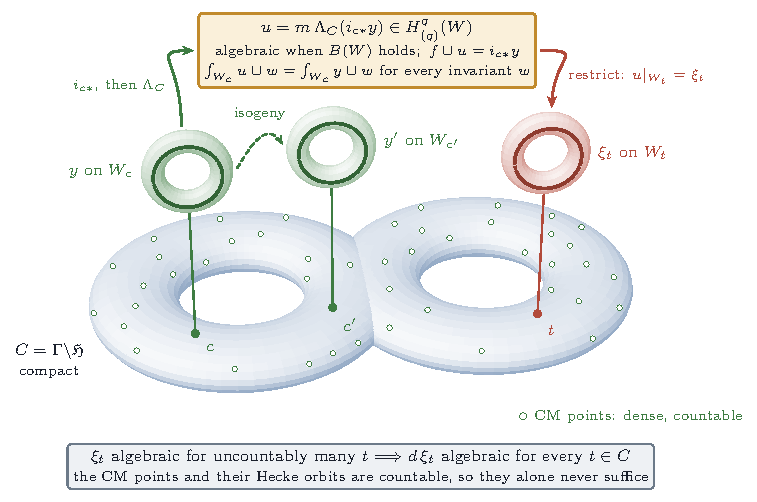
\includegraphics[width=0.84\textwidth]{fig_propagation}
\caption{\Cref{thm:lefschetzpropagation}(ii) along a compact Shimura curve
$C$. An algebraic class $y$ on one fibre, at a base point of a Weil family or
at a CM point of a Mumford family (hollow dots: the CM points, countable and
dense), is pushed into $W$ by the Gysin map and brought back to the invariant
summand by the base operator $\Lambda_{C}$. When $B(W)$ holds the result $u$
is an algebraic class on $W$, pinned down by the displayed pairing against the
invariant classes, and its restriction to a very general fibre is the
invariant part of $y$. The dashed arcs are isogenies between CM members along
Hecke orbits: they carry algebraic classes to algebraic classes but reach
only countably many points, and \Cref{lem:spreading}, in the box, needs
uncountably many. This is how \Cref{cor:weilequiv} and
\Cref{cor:mumfordequiv} turn each target into one case of \textup{(L)}.}
\label{fig:propagation}
\end{figure}

\begin{theorem}[The Mumford square at a CM point]\label{thm:mumfordcm}
Let $W\to C$ be a family as in \Cref{cor:mumfordlefschetz} and $c\in C$ a CM
point. Then every Hodge class on $X_{c}\times X_{c}$ is algebraic. In
particular the two exceptional classes of \Cref{prop:mumfordproduct} are
algebraic on $X_{c}\times X_{c}$.
\end{theorem}

\begin{proof}
The Hodge group $T$ of $X_{c}$ is a $\QQ$-torus contained in $G$. It lies in a
maximal $\QQ$-torus of $G=\Res_{F/\QQ}\SL_{1}(D)$, which is the restriction of
scalars of the norm one torus of a quadratic extension of $F$ inside $D$, of
rank three, one factor for each embedding of $F$. The cocharacter of the Hodge
structure lies in the factor of the embedding at which $D$ splits, and the
Galois group permutes the embeddings of $F$ transitively, so the smallest
$\QQ$-subtorus containing it has rank three: $T_{\CC}$ is a maximal torus of
$G_{\CC}\cong\SL_{2}^{3}$. Its eight weights on
$V=H^{1}(X_{c},\CC)=V_{1}\otimes V_{2}\otimes V_{3}$ are the vectors
$(\pm1,\pm1,\pm1)$, pairwise distinct. Hence
$\End^{0}(X_{c})\otimes\CC=\End_{T}(V)$ is the algebra of diagonal matrices
in a weight basis $(x_{w})$. For $n\ge1$, $\operatorname{Hom}(X_{c}^{n},X_{c})
\otimes\CC$ is the space of $n$-tuples $(\varphi_{1},\dots,\varphi_{n})$ of
such matrices, acting by $x_{w}\mapsto x_{w}\otimes u_{w}$ with
$u_{w}=(\varphi_{1,w},\dots,\varphi_{n,w})\in\CC^{n}$, so the vectors $u_{w}$
can be prescribed independently. The Hodge classes of $X_{c}^{n}$, tensored
with $\CC$, are spanned by the products of vectors $x_{w}\otimes u$,
$u\in\CC^{n}$, in $\bigwedge^{*}(V\otimes\CC^{n})$ in which the weights $w$,
counted with multiplicity, sum to zero.

We show that for every $n\ge1$ the ring $\Hdg^{*}(X_{c}^{n})$ is generated by
pull-backs of Hodge classes of $X_{c}$ along homomorphisms $X_{c}^{n}\to
X_{c}$. Put $w_{1}=(1,1,1)$, $w_{2}=(1,-1,-1)$, $w_{3}=(-1,1,-1)$ and
$w_{4}=(-1,-1,1)$; the weights are the $\pm w_{i}$,
$w_{1}+w_{2}+w_{3}+w_{4}=0$, and any three of the $w_{i}$ are linearly
independent, so the integer relations among them are the multiples of
$(1,1,1,1)$. Let $\alpha_{i}$ and $\beta_{i}$ be the multiplicities of $w_{i}$
and $-w_{i}$ in a nonempty multiset of weights with sum zero. Then
$\alpha_{i}-\beta_{i}$ is independent of $i$; so either some $\alpha_{i}$ and
$\beta_{i}$ are both positive, or all $\alpha_{i}$ are positive, or all
$\beta_{i}$ are. In each case the multiset contains one of the sets
$\{w_{i},-w_{i}\}$, $\{w_{1},w_{2},w_{3},w_{4}\}$,
$\{-w_{1},-w_{2},-w_{3},-w_{4}\}$, each of sum zero, and by induction every
product above is, up to sign, a product of monomials
$\bigwedge_{w\in P}(x_{w}\otimes u_{w})$ over such sets $P$, whose weights are
pairwise distinct. Choosing $f\in\Hom(X_{c}^{n},X_{c})\otimes\CC$ with
$f^{*}x_{w}=x_{w}\otimes u_{w}$ for $w\in P$ gives
$\bigwedge_{w\in P}(x_{w}\otimes u_{w})=f^{*}\bigl(\bigwedge_{w\in P}x_{w}\bigr)$,
with $\bigwedge_{w\in P}x_{w}$ a Hodge class of $X_{c}$ tensored with $\CC$.
The map $f\mapsto f^{*}(t)$ is polynomial and the rational homomorphisms are
Zariski dense in their complexification, so the same span is reached with $f$
defined over $\QQ$ and $t$ rational. The Hodge classes of the abelian fourfold
$X_{c}$ are algebraic because the Hodge conjecture holds for abelian fourfolds
\cite{Mar25a}, and pull-backs and products of algebraic classes are
algebraic. The case $n=2$ is the theorem.
\end{proof}

\begin{corollary}[The first classes beyond the Weil lines are one case of
\textup{(L)}]\label{cor:mumfordequiv}
Let $W\to C$ be as in \Cref{cor:mumfordlefschetz} and
$W^{(2)}=W\times_{C}W\to C$, an abelian scheme of relative dimension eight
with $W^{(2)}$ projective of dimension nine. The following are equivalent.
\begin{enumerate}[label=\textup{(\alph*)},leftmargin=2.6em,itemsep=2pt]
\item $B(W^{(2)})$ holds for the class $L_{W^{(2)}}$.
\item The two exceptional classes of $X_{t}\times X_{t}$ are algebraic for
  uncountably many $t\in C$.
\item The Hodge conjecture holds for $X_{t}\times X_{t}$ for every $t\in C$.
\item The Hodge conjecture holds for $W^{(2)}$; for this item $C$ is taken to
  be the compact Shimura curve of torsion-free level, or a finite \'etale
  cover of it.
\end{enumerate}
\end{corollary}

\begin{proof}
As in the proof of \Cref{cor:mumfordlefschetz}, the connected monodromy group
is $G$, so the monodromy invariants in $H^{*}(X_{t}\times X_{t},\QQ)$ are
contained in the $G$-invariants, which are the Hodge classes of
$X_{t}\times X_{t}$ for $t$ very general; conversely a $G$-invariant class is
flat, being fixed by the monodromy. The Hodge group of every fibre lies in
$G$, so the invariant classes are Hodge classes on every fibre. At a point $t$
that is not a CM point the Hodge group $H_{t}$ of $X_{t}$ is $G$. Indeed, if
$H_{t}$ were smaller, the Hodge classes of the powers of $X_{t}$ that are not
$G$-invariant would stay Hodge only on a discrete subset of the period
domain, the upper half plane; every point of the orbit of the Hodge structure
at $t$ under $H_{t}(\RR)^{+}$ carries them, so that orbit is a point, the
cocharacter of the Hodge structure is central in $H_{t}$, and $H_{t}$, the
smallest $\QQ$-group containing it, is a torus: $t$ would be a CM point. So
at such $t$ the Hodge classes of $X_{t}\times X_{t}$ are the invariant ones,
and $\End^{0}(X_{t})=\End_{G}(V)=\QQ$, because
$V\otimes\bar{\QQ}=V_{1}\otimes V_{2}\otimes V_{3}$ is an irreducible
representation of $G$; thus $X_{t}$ is as in \Cref{setup:mumford}.

(c) implies (b) trivially. (b) implies (c): the exceptional classes are
invariant, hence flat, so by \Cref{lem:spreading} a multiple of each is the
restriction of an algebraic class on $W^{(2)}$, and they are algebraic on
every fibre. At a point that is not a CM point, \Cref{thm:mumfordpowers} with
$n=2$ makes every Hodge class of $X_{t}\times X_{t}$ algebraic; at a CM point
this is \Cref{thm:mumfordcm}. (c) implies (a): by (c) every invariant class is
algebraic on every fibre, so by \Cref{lem:spreading} a multiple of it is the
restriction of an algebraic class on $W^{(2)}$, and
\Cref{thm:lefschetzfamily} gives $B(W^{(2)})$. (a) implies (c): at a CM point
$c_{0}$ every Hodge class of $X_{c_{0}}\times X_{c_{0}}$ is algebraic by
\Cref{thm:mumfordcm}, so by \Cref{thm:lefschetzpropagation}(iii) every
invariant class is the restriction of an algebraic class, and is algebraic on
every fibre. This is (c) at the points that are not CM points, where the
Hodge classes are the invariant ones; at a CM point (c) is
\Cref{thm:mumfordcm}.

For (d), split $H^{*}(W^{(2)},\QQ)$ into the summands $H^{p}(C,R^{q})$,
$p\in\{0,1,2\}$, as in the proof of \Cref{prop:mumfordfivefold}. The summands
with $p=1$ carry no Hodge class, by the argument given there, applied to the
fibre square. Those with $p=2$ are $f\cup H^{q}_{(q)}$, and
$f\cup u=i_{c*}(u|_{W^{(2)}_{c}})$ for any $c$; taking $c$ a CM point, where
$u|_{W^{(2)}_{c}}$ is a Hodge class and so algebraic by \Cref{thm:mumfordcm},
they are algebraic. The summands with $p=0$ are the invariants, all of Hodge
type. So (d) holds exactly when every invariant class is the restriction of an
algebraic class, which by \Cref{thm:lefschetzpropagation}(iii), applied at a
CM point, is (a).
\end{proof}

\begin{corollary}[One Weil family is one case of \textup{(L)}]
\label{cor:weilequiv}
Keep \Cref{setup:shimura}, let $s_{0}\in\cS$ be the image of a base point of
\Cref{thm:everyfamily}, and let $t_{1}\in\cS$ lie outside every proper
Zariski closed set $\Sigma_{\underline{P},\underline{q}}$ of
\Cref{thm:closedlocus}. Let $\kappa\colon C\to\cS$ be a morphism from a smooth
projective connected curve whose image contains $s_{0}$ and $t_{1}$, and
$W_{C}=\cA\times_{\cS}C$.
\begin{enumerate}[label=\textup{(\roman*)},leftmargin=2.6em,itemsep=2pt]
\item If $B(W_{C})$ holds for $L_{W_{C}}$, then $\Sigma=\cD_{n,n}$, and the
  Hodge conjecture holds in every degree for every member of the family with
  $\Hg(A)=\SU(V,H)$.
\item Conversely, if $\Sigma=\cD_{n,n}$ and the monodromy of $W_{C}$ is Zariski
  dense in $\SU(V,H)$, then $B(W_{C})$ holds for $L_{W_{C}}$.
\end{enumerate}
\end{corollary}

\begin{proof}
(i) The class $\kappa^{*}\omega$ is a global section of
$R^{2n}\pi_{*}\QQ$ on $C$, algebraic at a point over $s_{0}$ by
\Cref{thm:everyfamily}. By \Cref{thm:lefschetzpropagation}(ii) it is algebraic
at a point over $t_{1}$, so $t_{1}$ lies in some closed set
$\Sigma_{\underline{P},\underline{q}}$, which is therefore all of $\cS$.
\Cref{thm:closedlocus} gives $\Sigma=\cD_{n,n}$, and \Cref{thm:residual}(a)
the rest. (ii) With dense monodromy the invariants are the
$\SU(V,H)$-invariants, which are the Hodge classes of a member with
$\Hg(A)=\SU(V,H)$: the powers of the polarisation and the Weil classes, by
\Cref{thm:hdgcount}. All are algebraic on every fibre when
$\Sigma=\cD_{n,n}$, so they are restrictions of algebraic classes by
\Cref{lem:spreading}, and \Cref{thm:lefschetzfamily} applies.
\end{proof}

Curves $\kappa$ as in \Cref{cor:weilequiv} exist: the Baily--Borel
compactification of $\cS$ is projective \cite{BB66}, its boundary has
codimension $2n-1\ge3$, the rational boundary components of the domain of type
$\mathrm{I}_{n,n}$ being of type $\mathrm{I}_{n-r,n-r}$ with $r\ge1$, and a
general complete intersection curve through $s_{0}$ and $t_{1}$ avoids it.

\begin{theorem}[Two branches cannot be two objects]\label{thm:nosum}
Let $A$ be of $(K,-1,n)$-Weil type with $n\ge2$, $\omega\ne0$ a rational class
on the Weil line, and $E$ a perfect complex with $\ch(E)=N\omega$, $N\ne0$, and
$\sigma_{E}$ injective. Let
$E\cong\bigoplus_{i}F_{i}[k_{i}]$ be any decomposition. Then every summand
$F_{i}$ with $\ch(F_{i})\ne0$ has a Yoneda product
$\bigwedge^{2}\Ext^{1}(F_{i},F_{i})\to\Ext^{2}(F_{i},F_{i})$ that is not
injective. In particular $E$ is not a direct sum of shifts of line bundles,
of skyscraper sheaves of points, or of their images under autoequivalences of
$D^{b}(A)$, since the Ext algebra of each of these is the exterior algebra on
its $\Ext^{1}$.
\end{theorem}

\begin{proof}
By \Cref{thm:p2numerical}(ii) the kernel of $\operatorname{ev}_{E}$ in degree
two is $P\wedge Q$. The characteristic morphism is compatible with the
decomposition, so $\operatorname{ev}_{F_{i}}(p\wedge q)=
\operatorname{ev}_{F_{i}}(p)\operatorname{ev}_{F_{i}}(q)=0$ for all
$p\in P$ and $q\in Q$. Suppose the Yoneda product of $F=F_{i}$ is injective on
$\bigwedge^{2}\Ext^{1}$. Then the images $\bar P$ and $\bar Q$ of $P$ and $Q$
in $\Ext^{1}(F,F)$ satisfy $\bar p\wedge\bar q=0$ for all $\bar p,\bar q$, so
either $\bar P=0$, or $\bar Q=0$, or $\bar P=\bar Q$ is a line. In the first
case $\operatorname{ev}_{F}$ kills $P\wedge HH^{1}$, in the second
$Q\wedge HH^{1}$, in the third all of $HH^{2}=HH^{1}\wedge HH^{1}$; by the
compatibility $\sigma_{F}\circ\operatorname{ev}_{F}=(\,\cdot\,)\lrcorner
\ch(F)$ of \Cref{setup:hh} the same subspace annihilates $x=\ch(F)$.

These annihilators are computed in the free module of rank one that
$H^{*}(A,\CC)$ is over $HH^{*}(A)=\bigwedge^{*}(P\oplus Q)$, with generator the
holomorphic volume form $\Omega$: an element $y\cdot\Omega$ is killed by
$P\wedge HH^{1}$ exactly when $p\wedge y$ has top degree for every $p\in P$,
that is when $y\in\det P\wedge\bigwedge^{*}Q+\bigwedge^{\ge4n-1}(P\oplus Q)$.
Since $\det P\cdot\Omega=\pm\alpha_{+}$, the first summand gives the classes
$\bigwedge^{j}Q\cdot\alpha_{+}$, of type $(n-b,n+a)$ with $a$ wedges by
$V_{-}^{0,1}$ and $b$ contractions by $T_{+}$, and the second gives classes of
type $(1,2n)$, $(0,2n-1)$ and $(0,2n)$. The components of $x$ are of type
$(k,k)$, so $x\in\CC\alpha_{+}$. Symmetrically the second case gives
$x\in\CC\alpha_{-}$ and the third $x=0$. Finally $x$ is
rational, complex conjugation carries $V_{+}$ to $V_{-}$ and $H^{1,0}$ to
$H^{0,1}$, so $\bar\alpha_{+}\in\CC\alpha_{-}$, and a rational multiple of
$\alpha_{+}$ or of $\alpha_{-}$ is zero. So $\ch(F)=0$. As
$\sum_{i}(-1)^{k_{i}}\ch(F_{i})=N\omega\ne0$, some summand has nonzero
Chern character, and the first statement follows; the second is the special
case in which every summand has an exterior Ext algebra.
\end{proof}

\subsection{Which hypotheses suffice}
\label{ssec:closure}

The implications proved above, together with those of \Cref{ssec:bullseye},
determine exactly which combinations of statements yield the conjecture. The
logical skeleton of the paper and of the literature it quotes is finite: a
set of statements, each of them proved here, quoted from the literature, or
taken as a hypothesis, and a set of inference rules, each of them one
theorem. Consequences can then be taken.

The answer is only as strong as the rule set. A set of statements the rules
do not carry to the conjecture is \emph{insufficient} in the sense of the
rules, and that means no more than that no rule derives the conjecture from
it. An implication that is true and left out makes a set look necessary when
it is not. One such implication
is elementary, and it decides the shape of the answer, so we prove it first.

\begin{proposition}[The conjecture for the varieties that are not abelian
is the conjecture]\label{prop:f3ishc}
Let $A$ be a complex abelian variety of dimension $g\ge1$ and let
$X=A\times\PP^{1}$. Then $X$ is a smooth complex projective variety that is
not an abelian variety, and if every Hodge class of degree $2p$ on $X$ is
algebraic, then so is every Hodge class of degree $2p$ on $A$. Consequently
the statement
\begin{quote}
the Hodge conjecture holds for every smooth complex projective variety that
is not an abelian variety
\end{quote}
implies the Hodge conjecture for every abelian variety, and it is equivalent
to $\mathbf{HC}$.
\end{proposition}

\begin{proof}
$X$ is smooth and projective of dimension $g+1$. By the K\"unneth formula
$h^{1,0}(X)=h^{1,0}(A)+h^{1,0}(\PP^{1})=g$, while an abelian variety of
dimension $g+1$ has $h^{1,0}=g+1$; so $X$ is not an abelian variety. (Equally,
$X$ contains the rational curves $\{a\}\times\PP^{1}$, and every morphism
from $\PP^{1}$ to a complex torus is constant, since it lifts to the
universal cover $\CC^{g+1}$ \cite[Chapter~1]{BL04}.)

Let $\mathrm{pr}\colon X\to A$ be the projection and $D=A\times\{0\}$, a
smooth divisor that $\mathrm{pr}$ maps isomorphically onto $A$, so that
$\mathrm{pr}_{*}[D]=1$ in $H^{0}(A,\QQ)$. Let $\alpha$ be a Hodge class of
degree $2p$ on $A$. Pull-back along a morphism is a morphism of Hodge
structures, so $\mathrm{pr}^{*}\alpha$ is a Hodge class of degree $2p$ on
$X$, and by hypothesis $\mathrm{pr}^{*}\alpha=[Z]$ for an algebraic cycle
$Z$ on $X$ with rational coefficients. The projection formula gives
\[
  \mathrm{pr}_{*}\bigl([Z]\cup[D]\bigr)
  =\mathrm{pr}_{*}\bigl(\mathrm{pr}^{*}\alpha\cup[D]\bigr)
  =\alpha\cup\mathrm{pr}_{*}[D]=\alpha .
\]
The cycle class map is compatible with intersection products and with proper
push-forward \cite[Chapter~19]{Ful98}, so the left side
is the class of the cycle $\mathrm{pr}_{*}(Z\cdot D)$ and $\alpha$ is
algebraic. A point, the abelian variety of dimension zero, satisfies the
conjecture trivially.

So the displayed statement gives the conjecture for every abelian variety,
and with it the conjecture for every smooth complex projective variety. The
converse is immediate: the displayed statement is a special case of
$\mathbf{HC}$.
\end{proof}

Since the conjecture for the varieties that are not abelian is the whole
conjecture, the statement that belongs on a frontier is weaker: it asks for
algebraicity only modulo what abelian varieties supply.

\begin{definition}[The conjecture modulo abelian varieties]
\label{def:f3prime}
For a smooth complex projective variety $X$ and $p\ge0$ let
$\mathrm{Ab}^{p}(X)\subseteq H^{2p}(X,\QQ)$ be the span of the classes
$\Gamma_{*}\gamma=\mathrm{pr}_{X*}\bigl([\Gamma]\cup\mathrm{pr}_{B}^{*}\gamma\bigr)$
of degree $2p$, where $B$ runs over the complex abelian varieties, the point
included, $\gamma$ over the Hodge classes on $B$, and $\Gamma$ over the
algebraic cycles on $B\times X$ with rational coefficients. The statement
\textup{(F3$'$)} is: for every $X$ and every $p$,
\[
  \Hdg^{p}(X)=\mathrm{Ab}^{p}(X).
\]
\end{definition}

Each $\Gamma_{*}\gamma$ is a Hodge class, since cup product with an
algebraic class and push-forward preserve Hodge classes, so
$\mathrm{Ab}^{p}(X)\subseteq\Hdg^{p}(X)$; and taking $B$ a point shows that
$\mathrm{Ab}^{p}(X)$ contains every algebraic class. So \textup{(F3$'$)} says
that every Hodge class is algebraic modulo the images of Hodge classes of
abelian varieties under algebraic correspondences, which is the form of (F3)
that \Cref{rem:f3collapse} asks for.

\begin{proposition}[What is known of \textup{(F3$'$)}]\label{prop:f3prime}
\leavevmode
\begin{enumerate}[label=\textup{(\roman*)},leftmargin=2.6em]
\item $\mathbf{HC}$ implies \textup{(F3$'$)}, and \textup{(F3$'$)} together
  with the conjecture for abelian varieties implies $\mathbf{HC}$.
\item \textup{(F3$'$)} holds on every abelian variety and on every product
  $A\times\PP^{1}$ with $A$ abelian; the argument of \Cref{prop:f3ishc} gives
  nothing for it.
\item Let $\mathcal{A}$ be the class of smooth complex projective varieties
  $X$ for which $H^{*}(X,\QQ)$ is spanned by classes $\Gamma_{*}y$ with $B$
  abelian, $\Gamma$ an algebraic cycle on $B\times X$ and
  $y\in H^{*}(B,\QQ)$. Every $X\in\mathcal{A}$ satisfies \textup{(F3$'$)}.
  The class $\mathcal{A}$ contains every abelian variety and every smooth
  projective curve, and it is closed under products and under images of
  surjective morphisms. So it contains every product of curves, every
  symmetric product of a curve, and every smooth projective variety onto
  which a product of curves or an abelian variety maps surjectively.
\item Every $X$ of dimension $n$ satisfies \textup{(F3$'$)} in the degrees
  $2p$ with $p\in\{0,1,n-1,n\}$, so every $X$ of dimension at most three
  satisfies it in every degree.
\end{enumerate}
\end{proposition}

\begin{proof}
(i) If $\mathbf{HC}$ holds, then $\Hdg^{p}(X)$ consists of algebraic classes,
which lie in $\mathrm{Ab}^{p}(X)$. Conversely, if the conjecture holds for
abelian varieties, every $\gamma$ in \Cref{def:f3prime} is algebraic, so
every $\Gamma_{*}\gamma$ is, since composition with a correspondence carries
algebraic classes to algebraic classes \cite[Chapter~16]{Ful98}; then
\textup{(F3$'$)} says that every Hodge class is algebraic.

(ii) On an abelian variety $A$ take $B=A$ and $\Gamma$ the diagonal. On
$X=A\times\PP^{1}$ the K\"unneth formula gives
$H^{*}(X,\QQ)=\mathrm{pr}^{*}H^{*}(A,\QQ)\oplus
\mathrm{pr}^{*}H^{*}(A,\QQ)\cup\eta$, with $\eta$ the class of a point of
$\PP^{1}$ pulled back to $X$, which is algebraic. The first summand is
$\Gamma_{*}H^{*}(A,\QQ)$ for $\Gamma$ the transpose of the graph of
$\mathrm{pr}$, and the second is $\Gamma'_{*}H^{*}(A,\QQ)$ for
$\Gamma'=\Gamma\cdot\mathrm{pr}_{X}^{*}\eta$. So $X\in\mathcal{A}$, and
(iii) applies.

(iii) Let $X\in\mathcal{A}$ and fix $p$. Since $H^{2p}(X,\QQ)$ is finite
dimensional, finitely many classes $\Gamma_{j*}y_{j}$ span it, and we may
take each $\Gamma_{j}$ of pure codimension $c_{j}$ on $B_{j}\times X$ and each
$y_{j}$ of pure degree $k_{j}$, with $k_{j}+2c_{j}-2\dim B_{j}=2p$. Then
$\Gamma_{j*}\colon H^{k_{j}}(B_{j},\QQ)\to H^{2p}(X,\QQ)$ is a morphism of
Hodge structures up to a Tate twist, and the sum of these maps is a
surjective morphism of polarisable Hodge structures onto $H^{2p}(X,\QQ)$.
Polarisable Hodge structures are semisimple, so its kernel has a complement
that is a sub-Hodge structure and maps isomorphically onto $H^{2p}(X,\QQ)$;
hence every Hodge class of degree $2p$ is the image of a Hodge class, that is
$\sum_{j}\Gamma_{j*}\gamma_{j}$ with each $\gamma_{j}$ a Hodge class on
$B_{j}$. So $\Hdg^{p}(X)=\mathrm{Ab}^{p}(X)$.

An abelian variety lies in $\mathcal{A}$ through its diagonal. A curve $C$
of genus $g\ge1$ lies in $\mathcal{A}$ through an Abel--Jacobi embedding
$\iota\colon C\to J(C)$: the transpose of its graph induces $\iota^{*}$,
which is an isomorphism on $H^{0}$ and $H^{1}$ and sends the class of the
theta divisor to $g$ times the class of a point, so it is surjective; the
projective line is the image of an elliptic curve under a double cover, and
is covered by the last closure property. For products, if $H^{*}(X_{i},\QQ)$
is spanned by the $\Gamma_{i*}y$, then by the K\"unneth formula
$H^{*}(X_{1}\times X_{2},\QQ)$ is spanned by the
$(\Gamma_{1}\times\Gamma_{2})_{*}(y_{1}\otimes y_{2})$, with
$\Gamma_{1}\times\Gamma_{2}$ an algebraic cycle on
$(B_{1}\times B_{2})\times(X_{1}\times X_{2})$. For images, let
$f\colon Y\to X$ be a surjective morphism with $Y\in\mathcal{A}$, let
$r=\dim Y-\dim X$ and let $h$ be an ample class on $Y$. The correspondence
$\Psi=[\Gamma_{f}]\cdot\mathrm{pr}_{Y}^{*}h^{r}$ on $Y\times X$ induces
$\Psi_{*}y=f_{*}(y\cup h^{r})$, and
$\Psi_{*}f^{*}x=x\cup f_{*}h^{r}=c\,x$ with $c>0$ the degree of $h^{r}$ on a
general fibre. So $\Psi_{*}$ is surjective, and $H^{*}(X,\QQ)$ is spanned by
the classes $(\Psi\circ\Gamma)_{*}y$, with $\Psi\circ\Gamma$ algebraic
\cite[Chapter~16]{Ful98}. A symmetric product of a curve is the image of a
power of it.

(iv) Every class of degree $0$ or $2n$ is algebraic, and every Hodge class of
degree $2$ is algebraic by the Lefschetz theorem on $(1,1)$ classes. For
$n\ge2$, the hard Lefschetz theorem makes cup product with $h^{n-2}$, for $h$
an ample class, an isomorphism $H^{2}(X,\QQ)\to H^{2n-2}(X,\QQ)$ of Hodge
structures up to a Tate twist, so every Hodge class of degree $2n-2$ is
$h^{n-2}$ times a Hodge class of degree $2$, and is algebraic. Algebraic
classes lie in $\mathrm{Ab}^{p}(X)$. When $n\le3$ every $p$ between $0$ and
$n$ is one of $0,1,n-1,n$.
\end{proof}

\begin{remark}[The reach of algebraic correspondences]\label{rem:f3primeopen}
\textup{(F3$'$)} is the statement that the Hodge conjecture reduces to
abelian varieties along algebraic correspondences, and
\Cref{prop:f3prime} records the cases of such a reduction that are theorems:
the varieties of $\mathcal{A}$, whose whole cohomology is reached from abelian
varieties by algebraic correspondences, and the degrees in which the
conjecture itself is a theorem. The next degree is degree four on fourfolds
outside $\mathcal{A}$ and outside the scope of \Cref{prop:f3primesmall} and
\Cref{prop:f3primefibration}. The square $S\times S$ of a K3 surface is the standard
example when $\End_{\mathrm{Hdg}}(T(S))$ is a totally real field of degree
at least two, that is, when $S$ has real multiplication. When that field is
$\QQ$ or a CM field, the Hodge conjecture holds on $S\times S$: by
\Cref{prop:orthpowers}(i) in the first case, and in the second by
\cite{Bus19} and the fact that the elements of norm one span a CM field, as in
\cite{RM08} (\Cref{prop:k3powers}). Its Hodge classes in
$H^{2}(S)\otimes H^{2}(S)$ include the classes
that induce the Hodge endomorphisms of the transcendental lattice $T(S)$, and
$S\times S$ lies in $\mathcal{A}$ as soon as the Kuga--Satake embedding of
$T(S)$ is induced by an algebraic cycle, the Kuga--Satake Hodge conjecture for
$S$: the transpose of such a cycle maps the
cohomology of the Kuga--Satake variety onto $T(S)$, and the rest of
$H^{*}(S,\QQ)$ is algebraic. The rational Hodge isometries are algebraic
\cite{Bus19}, but a real multiplication is not an isometry, and
\Cref{rem:mumfordks} meets exactly this obstacle for the surfaces
$S_{\lambda}$. With the Hodge conjecture for products of K3 surfaces of
\cite{OAI26f} as hypothesis the obstacle disappears for K3 surfaces
(\Cref{cor:k3all}), and the step itself remains.

For varieties whose cohomology is not of abelian type the position is
starker. By \Cref{prop:noabeliantype} no correspondence moves the $H^{3}$ of a
very general quintic threefold into the cohomology of an abelian variety, so
such a variety does not lie in $\mathcal{A}$. That is no obstruction to
\textup{(F3$'$)} itself, since a Hodge class spans a Hodge structure of Tate
type, which is of abelian type, and nothing in Hodge theory forbids it from
lying in $\mathrm{Ab}^{p}(X)$. Nor is it a route: to put a Hodge class into
$\mathrm{Ab}^{p}(X)$ one must construct an algebraic cycle on $B\times X$
whose class carries it, which is the kind of construction the Hodge
conjecture asks for, now on $B\times X$ instead of on $X$. The cases of
\textup{(F3$'$)} proved below outside $\mathcal{A}$ come from the Hodge
conjecture itself, from hypotheses on zero-cycles, and, in degree four, from
correspondences with members of $\mathcal{A}$
(\Cref{prop:k3powers} to \Cref{prop:f3primedominant}); none of them reaches a
variety in general position, and \textup{(F3$'$)} enters \Cref{thm:closure} as
a hypothesis.
\end{remark}

Two further facts fix the position of \textup{(F3$'$)}. The first says how
strong it is.

\begin{proposition}[The strength of \textup{(F3$'$)}]\label{prop:f3primestrength}
\textup{(F3$'$)} implies \textup{(M)}: every Hodge class on every smooth
complex projective variety is motivated in the sense of Andr\'e. In
particular it implies that every such class is absolutely Hodge. Adding the
implication $\textup{(F3$'$)}\Rightarrow\textup{(M)}$ to the rule set of
\Cref{setup:rules} leaves the five minimal sufficient sets of
\Cref{thm:closure}(ii) unchanged.
\end{proposition}

\begin{proof}
Let $\gamma\in\Hdg^{p}(X)$. By \textup{(F3$'$)},
$\gamma=\sum_{j}\Gamma_{j*}\beta_{j}$ with $\beta_{j}$ a Hodge class on an
abelian variety $B_{j}$ and $\Gamma_{j}$ an algebraic cycle on $B_{j}\times X$.
Every Hodge class on an abelian variety is motivated
\cite[Th\'eor\`eme~0.6.2]{And96b}, and the motivated classes form a graded
$\QQ$-algebra that contains the algebraic classes and is stable under
pull-back and push-forward along morphisms \cite[\S2]{And96b}. So
$\mathrm{pr}_{B_{j}}^{*}\beta_{j}\cup[\Gamma_{j}]$ is motivated, and so is its
push-forward $\Gamma_{j*}\beta_{j}$; hence $\gamma$ is motivated. Motivated
classes are absolutely Hodge \cite[\S2]{And96b}. For the last assertion,
the new rule has the premise (F3$'$) and the conclusion (M). The sets $C_{1}$
and $C_{2}$ of the proof of \Cref{thm:closure} omit (F3$'$), and $C_{3}$ and
$C_{4}$ contain both statements, so the four sets stay closed and that proof
applies without change; the five sets remain sufficient, since adding a rule
only enlarges closures.
\end{proof}

So on the route $\{\mathrm{L},\mathrm{F3}'\}$ the second member already
contains \textup{(M)}, and that route is never easier than
$\{\mathrm{L},\mathrm{M}\}$. The second fact locates, on the powers of a variety of orthogonal type,
the first class that \textup{(F3$'$)} has to reach.

\begin{proposition}[Powers of a variety of orthogonal type]
\label{prop:orthpowers}
Let $Y$ be a smooth complex projective variety of even dimension $m$. Suppose
that $H^{k}(Y,\QQ)$ is spanned by algebraic classes for $k\ne m$, that
$H^{m}(Y,\QQ)=N\oplus V$ with $N$ spanned by algebraic classes, the
intersection form $\psi$ nondegenerate on $N$ and $V=N^{\perp}$, and that the
Hodge group of $V$ is $\SO(V,\psi)$, with $t=\dim V\ge3$. Let
$\det(V)\in H^{mt}(Y^{t},\QQ)$ be the image of a generator of
$\bigwedge^{t}V\subseteq V^{\otimes t}$ under the K\"unneth embedding
$V^{\otimes t}\subseteq H^{mt}(Y^{t},\QQ)$.
\begin{enumerate}[label=\textup{(\roman*)},leftmargin=2.6em,itemsep=2pt]
\item The Hodge conjecture holds for $Y^{n}$ for every $n<t$.
\item $\det(V)$ is a Hodge class, and $\Hdg^{*}(Y^{t})$ is spanned by
  algebraic classes and $\det(V)$.
\item $\det(V)$ does not lie in the $\QQ$-algebra generated by the pull-backs
  along the projections of the Hodge classes of the $Y^{j}$, $j<t$.
\item The Hodge conjecture holds for every power of $Y$ if and only if
  $\det(V)$ is algebraic, and \textup{(F3$'$)} holds for every power of $Y$
  if and only if $\det(V)\in\mathrm{Ab}(Y^{t})$.
\end{enumerate}
\end{proposition}

\begin{proof}
Algebraic classes have even degree, so $H^{k}(Y,\QQ)=0$ for odd $k$. Let
$[\Delta]=\sum_{k}\pi_{k}$ be the K\"unneth decomposition of the class of the
diagonal, $\pi_{k}\in H^{2m-k}(Y,\QQ)\otimes H^{k}(Y,\QQ)$. For $k\ne m$,
$\pi_{k}=\sum_{i}e_{i}^{\vee}\otimes e_{i}$ for a basis $(e_{i})$ of
$H^{k}(Y,\QQ)$ and the Poincar\'e dual basis of $H^{2m-k}(Y,\QQ)$, both
spanned by algebraic classes, so $\pi_{k}$ is algebraic; likewise the part
$\pi_{N}$ of $\pi_{m}$ in $N\otimes N$, since $\psi$ is nondegenerate on $N$.
So $\pi_{V}=[\Delta]-\sum_{k\ne m}\pi_{k}-\pi_{N}$, the class of $\psi^{-1}$ in
$V\otimes V\subseteq H^{2m}(Y\times Y,\QQ)$, is algebraic.

The Hodge group of $Y^{n}$ is $\SO(V,\psi)$, acting on
$H^{*}(Y^{n},\QQ)=\bigl(H^{*}(Y,\QQ)\bigr)^{\otimes n}$ through the factors $V$
and trivially on the rest, which is spanned by algebraic classes; so the Hodge
classes are the $\SO(V)$-invariants. By the first fundamental theorem for the
special orthogonal group \cite[Chapter~5]{GW09}, the invariants of $\SO(V)$ in
$V^{\otimes j}$ are spanned by the complete contractions with $\psi^{-1}$ when
$j<t$, and, when $j=t$, by these and the determinant tensor; in general they
are spanned by products of contractions and determinant tensors on disjoint
sets of $t$ factors. A contraction of the factors $a$ and $b$ of $Y^{n}$ is the
pull-back of $\pi_{V}$ along the projection to those two factors, a
determinant on a set $I$ of $t$ factors is the pull-back of $\det(V)$ along
the projection to $Y^{I}$, and products of these with pull-backs of algebraic
classes span the Hodge classes. This gives (i), (ii) and the first half of
(iv). For (iii), the orthogonal group $\mathrm{O}(V,\psi)$ acts on
$H^{*}(Y^{j},\QQ)$ in the same way, and for $j<t$ every $\SO(V)$-invariant is
$\mathrm{O}(V)$-invariant; pull-backs along projections and cup products
commute with the diagonal action of $\mathrm{O}(V)$, so every element of the
algebra in (iii) is $\mathrm{O}(V)$-invariant, while a reflection acts on
$\det(V)$ by $-1$. For the second half of (iv), $\mathrm{Ab}^{*}(Y^{n})$
contains the algebraic classes and is stable under pull-back along projections
and under cup product: $\Gamma_{*}\gamma\cup\Gamma'_{*}\gamma'$ is the image of
$\gamma\otimes\gamma'$ on $B\times B'$ under the correspondence
$(\Gamma\times\Gamma')$ followed by the diagonal of $Y^{n}$.
\end{proof}

For a K3 surface $S$ with $\End_{\mathrm{Hdg}}(T(S))=\QQ$ the Hodge group of
$T(S)$ is $\SO(T(S))$ \cite{Zar83}; for a very general one, $t=21$. So the
Hodge conjecture holds for $S^{n}$ with $n\le20$, and on $S^{21}$ it is
equivalent to the algebraicity of the single class $\det(T(S))$. The argument
is the classical one from invariant theory, and we make no claim of priority
for it. What it adds here is the location of the first instance of
\textup{(F3$'$)} on the powers of such a variety that invariant theory does
not reach: one class, in one degree, on one power.

The same invariant theory, with the motivic decompositions of the
literature and the theorems of Buskin and Markman on Hodge isometries, gives
the Hodge conjecture itself, and so \textup{(F3$'$)}, on the other varieties
built from a K3 surface and on varieties of K3$^{[n]}$ type, up to a real
multiplication and one determinant class.

\begin{proposition}[Powers, Hilbert schemes and moduli spaces of a K3
surface]\label{prop:k3powers}
Let $S$ be a projective K3 surface, $T=T(S)_{\QQ}$, $t=\dim T$ and
$E=\End_{\mathrm{Hdg}}(T)$, a totally real field or a CM field \cite{Zar83}.
\begin{enumerate}[label=\textup{(\roman*)},leftmargin=2.6em,itemsep=2pt]
\item If $E$ is a CM field, the Hodge conjecture holds for every power
  $S^{k}$ \cite[Theorem~5.4]{RM08}, \cite{Bus19}, hence for every Hilbert
  scheme $S^{[n]}$ \cite{dCM02}, for every smooth projective moduli space of
  Gieseker stable (twisted) sheaves on $S$, or of $\sigma$-stable objects in
  $D^{b}(S,\alpha)$ for a generic stability condition $\sigma$ and a Brauer
  class $\alpha$ \cite[Theorem~0.1, Remark~2.1]{Bue20}, and for the crepant
  resolutions of the ten-dimensional moduli spaces $M_{\sigma}(2v_{0})$ of
  $\sigma$-semistable objects in $D^{b}(S,\alpha)$, with $v_{0}$ primitive,
  $v_{0}^{2}=2$ and $\sigma$ $v_{0}$-generic \cite[Theorem~1.3]{FFZ21}.
\item If $E=\QQ$, the Hodge conjecture holds for $S^{[n]}$ for every
  $n<t(t+1)/2$, and for every moduli space $M$ as in \textup{(i)} with
  $\dim M<t$. For $N=t(t+1)/2$ the following are equivalent: the Hodge
  conjecture for $S^{[N]}$; the algebraicity of the class $\det(T)$ on $S^{t}$
  of \Cref{prop:orthpowers}; the Hodge conjecture for every power of $S$; and
  the Hodge conjecture for every $S^{[n]}$. For a very general $S$, the Hodge
  conjecture holds for $S^{[n]}$ with $n\le230$, and for $S^{[231]}$ if and
  only if $\det(T(S))$ on $S^{21}$ is algebraic.
\item If $E$ is totally real of degree at least two, the Hodge conjecture for
  $S\times S$, the Hodge conjecture for $S^{[2]}$, and the statement that
  every element of $E$ acts on $T$ through an algebraic cycle on $S\times S$
  are equivalent.
\end{enumerate}
Wherever the Hodge conjecture holds, so does \textup{(F3$'$)}. This is a
consequence of \cite{RM08,Bus19,dCM02,Bue20,FFZ21} and
\Cref{prop:orthpowers}; we make no claim of priority.
\end{proposition}

\begin{proof}
We use three facts. First, $H^{*}(S,\QQ)=A\oplus T$ with
$A=H^{0}\oplus\NS(S)_{\QQ}\oplus H^{4}$ spanned by algebraic classes; the
K\"unneth components of the diagonal of $S$ are algebraic \cite{Mur90}, and
so is its part $\pi_{T}$ in $T\otimes T$, as in the proof of
\Cref{prop:orthpowers}. The Hodge classes of $S^{k}$ are the invariants in
$(A\oplus T)^{\otimes k}$ of the Hodge group of $T$, which acts trivially on
$A$. Second, if $H^{*}(X,\QQ)$ is spanned by the images of the
$H^{*}(Y_{i},\QQ)$ under algebraic correspondences and the Hodge conjecture
holds for every $Y_{i}$, it holds for $X$: by the semisimplicity argument of
the proof of \Cref{prop:f3prime}(iii) every Hodge class of $X$ is a sum of
images of Hodge classes of the $Y_{i}$. Third, the correspondences
$\Gamma_{\nu}$ of the proof of \Cref{prop:aclosure}(ii) give an isomorphism
of Chow motives between $h(S^{[n]})$ and
$\bigoplus_{\nu}h(S^{(\nu)})(l(\nu)-n)$ \cite{dCM02}, so each
$h(S^{(\nu)})(l(\nu)-n)$ is a direct summand of $h(S^{[n]})$, and the lift
$\widetilde\Gamma_{\nu*}$ takes the same value on a class of $S^{l(\nu)}$ and
on its average over $G_{\nu}$. Hence the Hodge
conjecture holds for $S^{[n]}$ if and only if, for every partition $\nu$ of
$n$, every $G_{\nu}$-invariant Hodge class of $S^{l(\nu)}$ is algebraic. By
\cite[Theorem~0.1, Remark~2.1]{Bue20} the Chow motive of a moduli space $M$
as in (i) is a direct summand of a sum of Tate twists of motives
$h(S^{k_{i}})$ with $1\le k_{i}\le\dim M$, and by
\cite[Corollary~4.5]{FFZ21} the Chow motive of a crepant resolution as in (i)
lies in the tensor subcategory generated by $h(S)$, whose objects are direct
summands of sums of
Tate twists of the $h(S^{k})$, the dual of $h(S)$ being $h(S)(2)$.

(i) Over $\CC$ the Hodge group of $T$ is a product of groups
$\GL(W_{\sigma})$ acting on
$T_{\CC}=\bigoplus_{\sigma}(W_{\sigma}\oplus W_{\sigma}^{\vee})$
\cite{Zar83}, and by the first fundamental theorem for the general linear
group \cite[Chapter~5]{GW09} its invariants in $T_{\CC}^{\otimes b}$ are
spanned by products of contractions of one factor with another. Under the
isomorphism $\End(T)\cong T\otimes T$, $\varphi\mapsto\tau_{\varphi}=
\sum_{i}t_{i}^{\vee}\otimes\varphi(t_{i})$, with $(t_{i}^{\vee})$ the dual
basis of a basis $(t_{i})$ for the intersection form, the Hodge classes of
$T\otimes T$ are the $\tau_{\varphi}$ with $\varphi\in E$, and these
contractions lie in their complex span. The rational span of the products of
the $\tau_{\varphi}$ on pairs of factors has the same complexification as the
space of invariants, so the Hodge classes of $S^{k}$ are spanned by such
products and pull-backs of algebraic classes. For $u\in E$ with $u\bar u=1$
the map $\id_{\NS}\oplus u$ is a rational Hodge isometry of
$H^{2}(S,\QQ)$, since the adjoint of $u$ is $\bar u$ \cite{Zar83}; it is
induced by an algebraic cycle \cite{Bus19}, and composing that cycle with
$\pi_{T}$ on both sides gives $\tau_{u}$, which is therefore algebraic. The
elements of norm one span $E$. Indeed, write $E=E_{0}(y_{0})$ with
$y_{0}^{2}=-\delta$, $\delta\in E_{0}$, and let $y\in E$ with $\bar y=-y$; for
$s\in\QQ$ the element $u_{s}=(1+sy)(1-sy)^{-1}$ has norm one. A linear form
on $E$ vanishing on all $u_{s}$ gives a rational function of $s$ vanishing on
$\QQ$, so it vanishes on the coefficients $1$, $2y$, $2y^{2}$ of the expansion
of $u_{s}$ in powers of $s$. As $y$ runs over $E_{0}y_{0}$, the $y$ span
$E_{0}y_{0}$ and the $y^{2}=-a^{2}\delta$, $a\in E_{0}$, span $E_{0}$, since
$2a=(a+1)^{2}-a^{2}-1$. So every $\tau_{u}$, $u\in E$, is algebraic, and the
Hodge conjecture holds for every $S^{k}$; this is the argument of
\cite[Lemma~5.3, Theorem~5.4]{RM08}, which takes the algebraicity of the
isometries from Mukai's announcement; \cite{Bus19} proves it in general.
We use \cite{RM08} only when $E$ is a CM field: for a totally real $E$ the
invariants of the Hodge group are not generated by those of degree two, since
they include determinants, as \Cref{prop:orthpowers} shows for $E=\QQ$, and
the powers do not reduce to the square. The rest of (i) follows
from the second and third facts.

(ii) Here the Hodge group of $T$ is $\SO(T)$ \cite{Zar83}, and $t\ge3$,
since a Hodge structure of K3 type of dimension two has complex
multiplication. The Hodge conjecture holds for $S^{k}$, $k<t$, by
\Cref{prop:orthpowers}(i), which gives the assertion on $M$ by the second
fact. Let $\nu$ be a partition of $n$ with $a_{j}$ parts equal to $j$, so
that $G_{\nu}=\prod_{j}\mathfrak{S}_{a_{j}}$ permutes the factors of
$S^{l(\nu)}$ within blocks of sizes $a_{j}$, one block for each distinct part
size. By the proof of \Cref{prop:orthpowers}, the Hodge classes of
$S^{l(\nu)}$ are spanned by algebraic classes and by products
$\beta=\det_{I}\cup\gamma$, where $\det_{I}$ is the pull-back of $\det(T)$
along the projection to a set $I$ of $t$ factors and $\gamma$ is pulled back
from the other factors. If two factors of $I$ lie in one block, the
transposition in $G_{\nu}$ exchanging them fixes $\gamma$ and changes the
sign of the alternating class $\det_{I}$, all classes involved being of even
degree; so it takes $\beta$ to $-\beta$, and the average of $\beta$ over
$G_{\nu}$ is zero. If $\nu$ has fewer than $t$ distinct part sizes, every set
of $t$ factors meets some block twice, so a $G_{\nu}$-invariant Hodge class,
being its own average, is the average of an algebraic class, and is
algebraic. A partition with $t$ distinct part sizes has
$n\ge1+2+\dots+t=t(t+1)/2$, so by the third fact the Hodge conjecture holds
for $S^{[n]}$ when $n<t(t+1)/2$ (\Cref{fig:k3threshold}). For $n=N$ the
partition $(1,2,\dots,t)$ has
$l(\nu)=t$ and $G_{\nu}=1$, so the Hodge class $\det(T)$ of $S^{t}$ is
algebraic if the Hodge conjecture holds for $S^{[N]}$. If $\det(T)$ is
algebraic, the Hodge conjecture holds for every power of $S$ by
\Cref{prop:orthpowers}(iv), and for every $S^{[n]}$ by the second fact; and
the conjecture for $S^{t}$ contains the algebraicity of $\det(T)$. A very
general $S$ has $E=\QQ$ and $t=21$, and $N=231$.

(iii) The Hodge structure $T$ has no nonzero Hodge class, so the Hodge
classes of $A\otimes T$ and $T\otimes A$ vanish, and those of $S\times S$
are the algebraic classes and the $\tau_{\varphi}$, $\varphi\in E$. A cycle
inducing $\varphi$ on $T$, composed with $\pi_{T}$ on both sides, gives
$\tau_{\varphi}$, and $\tau_{\varphi}$ induces $\varphi$ on $T$; this proves
the equivalence for $S\times S$. By \cite{dCM02},
$h(S^{[2]})=h(S^{(2)})\oplus h(S)(-1)$, and the Hodge conjecture holds for
$S$. The exchange of the two factors takes $\tau_{\varphi}$ to
$\tau_{\varphi^{*}}$, and the adjoint involution of a totally real $E$ is
trivial \cite{Zar83}, so every $\tau_{\varphi}$ is invariant under
$\mathfrak{S}_{2}$ and the Hodge conjecture for $S^{[2]}$ asks for the same
classes as that for $S\times S$.
\end{proof}

\begin{figure}[tbp]
\centering
  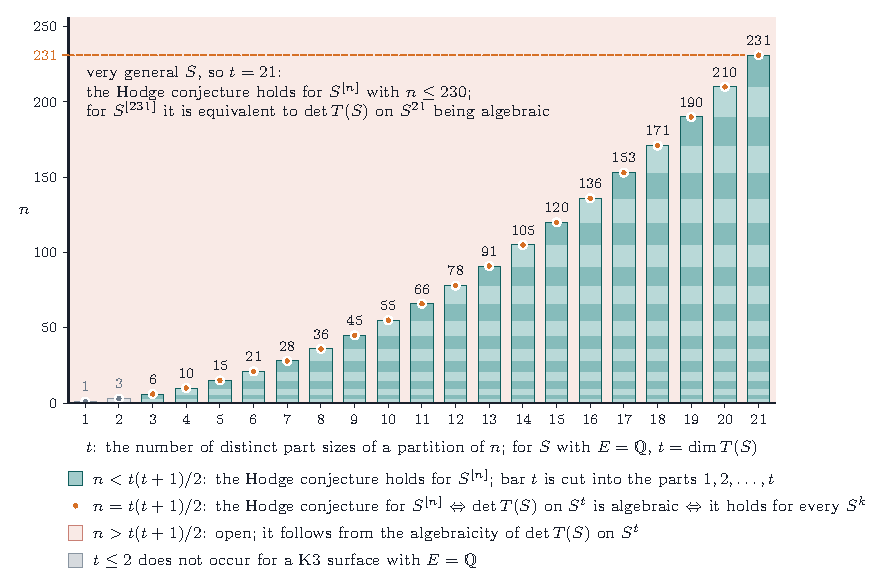
\includegraphics[width=\textwidth]{fig_k3threshold}
\caption{The threshold of \Cref{prop:k3powers}(ii). For $t=1,\dots,21$ the
bar rises to $t(t+1)/2$, the least $n$ that has a partition with $t$ distinct
part sizes, and is cut into the parts $1,2,\dots,t$ of the partition that
attains it. For a K3 surface $S$ with $E=\End_{\mathrm{Hdg}}(T(S))=\QQ$ and
$t=\dim T(S)$, which is at least $3$, the Hodge conjecture holds for
$S^{[n]}$ with $n$ below the bar; at its top it is equivalent to the
algebraicity of the class $\det T(S)$ on $S^{t}$ of \Cref{prop:orthpowers},
and to the Hodge conjecture for every power of $S$; above it, it follows
from that algebraicity. A very general $S$ has $t=21$: the
conjecture holds for $S^{[n]}$ with $n\le230$, and for $S^{[231]}$ it is
equivalent to the algebraicity of $\det T(S)$ on $S^{21}$, one of the
frontier cases of \textup{(F3$'$)} (\Cref{rem:f3primefrontier}).}
\label{fig:k3threshold}
\end{figure}

\begin{proposition}[Varieties of K3$^{[n]}$ type]\label{prop:k3ntype}
Let $X$ be a smooth projective hyperk\"ahler variety deformation equivalent
to the Hilbert scheme of $n\ge2$ points on a K3 surface, $q$ the
Beauville--Bogomolov form on $H^{2}=H^{2}(X,\QQ)$, $\NS=\NS(X)_{\QQ}$,
$T=\NS^{\perp}$ and $E=\End_{\mathrm{Hdg}}(T)$, a totally real field or a CM
field whose adjoint involution for $q$ is complex conjugation \cite{Zar83}.
Let $\mathrm{SH}(X)\subseteq H^{*}(X,\QQ)$ be the subalgebra generated by
$H^{2}$, and for $\varphi\in E$ with $\varphi^{*}=\varphi$ let
$c_{\varphi}=\sum_{i}t_{i}^{\vee}\cup\varphi(t_{i})\in H^{4}(X,\QQ)$, with
$(t_{i})$ a basis of $T$ and $(t_{i}^{\vee})$ its dual basis for $q$.
\begin{enumerate}[label=\textup{(\roman*)},leftmargin=2.6em,itemsep=2pt]
\item The Hodge classes of $\mathrm{SH}(X)$ are spanned by products of
  divisor classes and classes $c_{\varphi}$.
\item If $E$ is $\QQ$ or a CM field, every Hodge class of $\mathrm{SH}(X)$ is
  algebraic.
\item Let $n=2$. Then $\mathrm{SH}(X)=H^{*}(X,\QQ)$, with
  $b_{4}(X)=276=\dim\mathrm{Sym}^{2}H^{2}$, and $c_{2}(X)=\frac65q^{\vee}$,
  where $q^{\vee}\in\mathrm{Sym}^{2}H^{2}$ is dual to $q$. So the Hodge
  conjecture holds for $X$ when $E$ is $\QQ$ or a CM field. When $E$ is
  totally real of degree at least two, it holds for $X$ if and only if every
  element of $E$, acting on $T$ and by zero on $\NS$, is induced by an
  algebraic cycle on $X\times X$.
\end{enumerate}
This is a consequence of \cite{Mar24,CM13}; we make no claim of priority.
\end{proposition}

\begin{proof}
(i) Multiplication $\mathrm{Sym}^{k}H^{2}\to\mathrm{SH}^{2k}(X)$ is a
surjective morphism of polarisable Hodge structures, so by semisimplicity
every Hodge class of $\mathrm{SH}^{2k}(X)$ is the image of one of
$\mathrm{Sym}^{k}H^{2}=\bigoplus_{a+b=k}\mathrm{Sym}^{a}\NS\otimes
\mathrm{Sym}^{b}T$, whose Hodge classes are
$\mathrm{Sym}^{a}\NS\otimes(\mathrm{Sym}^{b}T)^{\Hdg}$. The isomorphism
$\End(T)\cong T\otimes T$ of the proof of \Cref{prop:k3powers}, now for $q$,
carries the adjoint to the exchange of the factors, so
$(\mathrm{Sym}^{2}T)^{\Hdg}$ consists of the tensors of the self-adjoint
$\varphi\in E$, whose images in $H^{4}$ are the $c_{\varphi}$. Over $\CC$ the
Hodge group of $T$ is a product of groups $\SO(T_{\sigma})$ on
$T_{\CC}=\bigoplus_{\sigma}T_{\sigma}$, with $\dim T_{\sigma}=\dim_{E}T\ge3$,
when $E$ is totally real, and of groups $\GL(W_{\sigma})$ on
$T_{\CC}=\bigoplus_{\sigma}(W_{\sigma}\oplus W_{\sigma}^{\vee})$ when $E$ is a
CM field \cite{Zar83}. By the first fundamental theorems
\cite[Chapter~5]{GW09}, the invariant polynomials of one vector of
$T_{\sigma}$, or of one vector of $W_{\sigma}$ and one of $W_{\sigma}^{\vee}$,
are generated by the quadratic form, or by the pairing: a determinant needs
$\dim T_{\sigma}$ distinct vectors. So $(\mathrm{Sym}^{b}T)^{\Hdg}\otimes\CC$
is spanned by products of elements of $(\mathrm{Sym}^{2}T)^{\Hdg}\otimes\CC$,
and the rational span of the products of classes $c_{\varphi}$, which has the
same complexification, is $(\mathrm{Sym}^{b}T)^{\Hdg}$.

(ii) Divisor classes are algebraic, so by (i) it suffices that every
$c_{\varphi}$ is. By \cite[Theorem~1.1]{CM13} the Lefschetz standard
conjecture holds for $X$, so the K\"unneth projectors and the inverse of the isomorphism
$L^{2n-2}\colon H^{2}\to H^{4n-2}$, $L$ the cup product with an ample class
$h$, are induced by algebraic cycles \cite{Kle68,Kle94}. Let $u\in E$ with
$u\bar u=1$, and $u=1$ if $E=\QQ$. The map $f_{u}=\id_{\NS}\oplus u$ is a
rational Hodge isometry of $H^{2}$, so by \cite[Theorem~1.1]{Mar24} there is
an algebraic class $Z_{u}$ on $X\times X$ (the diagonal if $u=1$) inducing on
$H^{2}$ a nonzero rational multiple of $f_{u}$: the class of the
correspondence $\tilde f$ of that theorem if it preserves degrees, and the
class of $\tilde f\circ(c_{2}(X)^{n-1}\cup\,\cdot\,)$ if it reverses them.
The class $Z_{u}$ may act in other degrees too; its K\"unneth component in
$H^{4n-2}(X)\otimes H^{2}(X)$ is algebraic and induces a nonzero multiple of
$f_{u}$ on $H^{2}$ and zero elsewhere. Applying $(L^{2n-2})^{-1}\otimes\id$
gives, up to a nonzero rational factor, the algebraic class
$\sum_{i}b_{i}\otimes f_{u}(a_{i})$, for a basis $(a_{i})$ of $H^{2}$ and
the dual basis $(b_{i})$ for $B(x,y)=\int_{X}xyh^{2n-2}$. Polarising the
relation $\int_{X}\alpha^{2n}=c_{X}q(\alpha)^{n}$ of Fujiki and Beauville
\cite{Bea83,Fuj87} gives
\[
  B(x,y)=\frac{c_{X}}{2n-1}\,q(h)^{n-2}\bigl(q(h)q(x,y)+2(n-1)q(x,h)q(y,h)\bigr),
\]
so $\NS$ and $T$ are orthogonal for $B$, and $B=\kappa q$ on $T$ with
$\kappa=c_{X}q(h)^{n-1}/(2n-1)\ne0$. With $(a_{i})$ adapted to
$\NS\oplus T$, the pull-back along the diagonal is
$\sum_{i}b_{i}\cup f_{u}(a_{i})=\nu+\kappa^{-1}c_{(u+\bar u)/2}$ with
$\nu\in\mathrm{Sym}^{2}\NS$ algebraic, because cup product on $H^{2}$ is
commutative and the exchange of factors turns $u$ into $\bar u$. So
$c_{(u+\bar u)/2}$ is algebraic. When $E$ is a CM field its elements of norm
one span it (proof of \Cref{prop:k3powers}(i)), so the $(u+\bar u)/2$ span
$E_{0}$, the self-adjoint part of $E$; when $E=\QQ$, $u=1$ suffices. So
every $c_{\varphi}$ is algebraic.

(iii) The variety $X$ has the Betti numbers of $S^{[2]}$, which by
\cite{dCM02} are those of $\mathrm{Sym}^{2}H^{*}(S)\oplus H^{*}(S)(-1)$:
$H^{\mathrm{odd}}(X)=0$ and $b_{4}(X)=253+1+22=276=\dim\mathrm{Sym}^{2}H^{2}$.
Here $c_{X}=3$, and the relation of Fujiki and Beauville gives
$\int_{X}abcd=q(a,b)q(c,d)+q(a,c)q(b,d)+q(a,d)q(b,c)$ for $a,b,c,d\in H^{2}$.
This form on $\mathrm{Sym}^{2}H^{2}$ is nondegenerate: in a $q$-orthogonal
basis $(e_{i})$ with $q(e_{i},e_{i})=d_{i}$, the $e_{i}e_{j}$ with $i<j$ are
orthogonal to each other and to the squares, with $\int_{X}(e_{i}e_{j})^{2}=
d_{i}d_{j}$, and on the squares the form has the matrix $D(J+2I)D$, with
$D=\mathrm{diag}(d_{i})$ and $J$ the matrix of ones, of determinant
$2^{22}\cdot25\prod_{i}d_{i}^{2}$. So
$\mathrm{Sym}^{2}H^{2}\to H^{4}$ is injective, hence bijective, and with
$H^{6}=h^{2}\cup H^{2}$ by the hard Lefschetz theorem,
$\mathrm{SH}(X)=H^{*}(X,\QQ)$. By \cite{Fuj87},
$\int_{X}c_{2}(X)xy=C\,q(x,y)$ for a constant $C$, and the Riemann--Roch
polynomial $\chi(L)=\binom{q(L)/2+3}{2}$ \cite{EGL01} gives $C=30$; the
Fujiki relation gives $\int_{X}q^{\vee}xy=25\,q(x,y)$, so
$c_{2}(X)=\frac65q^{\vee}$ by nondegeneracy. For $E=\QQ$ this makes
$c_{1}=q^{\vee}-q^{\vee}_{\NS}$ algebraic without \cite{CM13}, with
$q^{\vee}_{\NS}\in\mathrm{Sym}^{2}\NS$ the class dual to $q|_{\NS}$. With (i) and (ii) this proves the Hodge
conjecture for $X$ when $E$ is $\QQ$ or a CM field. Let $E$ be totally real
and $\varphi\in E$. If $\varphi\oplus0$ is induced by an algebraic cycle, the
computation of (ii) with $\varphi\oplus0$ in place of $f_{u}$ makes
$c_{\varphi}$ algebraic. Conversely, if $c_{\varphi}$ is algebraic, so is the
correspondence $x\mapsto(L^{2})^{-1}(c_{\varphi}\cup x)$. The Fujiki relation
gives $\int_{X}c_{\varphi}xy=\Tr(\varphi)q(x,y)+2q(\varphi x,y)$ for $x\in T$
and $y\in H^{2}$, and $B(z,y)=q(h)q(z,y)$ for $z\in T$, so that
correspondence acts on $T$ as $(\Tr(\varphi)+2\varphi)/q(h)$. The projector
onto $T$, the K\"unneth projector $\pi_{2}$ minus
$\sum_{j}n_{j}^{\vee}\otimes n_{j}$ over a basis $(n_{j})$ of $\NS$ and the
Hodge classes $n_{j}^{\vee}\in H^{6}$ dual to it, is algebraic by
\Cref{prop:f3prime}(iv); composing with it, $\varphi\oplus0$ is induced by an
algebraic cycle. By (i) the Hodge conjecture for $X$ is the algebraicity of
the $c_{\varphi}$, which proves the equivalence.
\end{proof}

For varieties of generalised Kummer type every Hodge class in the subalgebra
generated by $H^{2}$ is algebraic, whatever the field, and the Hodge
conjecture holds in dimension four \cite{FV25}. The preprint \cite{OG26}
announces, with \cite{Mar24}, that rational Hodge isometries between
varieties of the types K3$^{[a_{1}^{2}+1]}$ and K3$^{[a_{2}^{2}+1]}$ are
induced by algebraic cycles; it is not used here.

\begin{corollary}[Cubic fourfolds and their Fano varieties of lines]
\label{cor:fanolines}
Let $Y\subset\PP^{5}$ be a smooth cubic fourfold, $T(Y)\subset
H^{4}(Y,\QQ)$ the orthogonal complement of the Hodge classes,
$E(Y)=\End_{\mathrm{Hdg}}(T(Y))$, and $F=F(Y)$ the Fano variety of lines on
$Y$. The Hodge conjecture for $F$, the Hodge conjecture for $Y\times Y$, and
the statement that every element of $E(Y)$ acts on $T(Y)$ through an
algebraic cycle on $Y\times Y$ are equivalent. They hold when $E(Y)$ is $\QQ$
or a CM field, for instance when $Y$ is very general.
\end{corollary}

\begin{proof}
The Hodge conjecture holds for $Y$ \cite{Zuc77}, and also by
\Cref{prop:f3primesmall}, since $Y$ is covered by lines. So $H^{*}(Y,\QQ)$
is $T(Y)$ plus a space spanned by algebraic classes, on which the intersection
form is nondegenerate by the Hodge--Riemann relations, and as in the proof of
\Cref{prop:orthpowers} the part $\pi_{T}$ of the diagonal in
$T(Y)\otimes T(Y)$ is algebraic. The Hodge structure $T(Y)$ is of K3 type up
to a Tate twist and has no nonzero Hodge class, so $E(Y)$ is a field
\cite{Zar83}, and as in \Cref{prop:k3powers}(iii) the Hodge conjecture for
$Y\times Y$ is the third statement. By \cite{BD85}, $F$ is a hyperk\"ahler
fourfold of K3$^{[2]}$ type, and the universal line $P\subset F\times Y$
induces an isomorphism of Hodge structures $\alpha=P_{*}\colon
H^{4}(Y,\QQ)\to H^{2}(F,\QQ)$ up to a Tate twist. Both $T(Y)$ and $T(F)$
are the sums of the isotypic components that are not of Tate type, so
$\alpha(T(Y))=T(F)$ and $E(F)=\alpha E(Y)\alpha^{-1}$. Let $g$ be the
Pl\"ucker class on $F$ and $e=P^{t}_{*}\circ(g^{2}\cup\,\cdot\,)
\circ\alpha$, an algebraic correspondence that maps $T(Y)$ to itself, so that
$e|_{T(Y)}\in E(Y)$. For $0\ne\sigma\in H^{3,1}(Y)$,
$\int_{Y}e(\sigma)\bar\sigma=\int_{F}g^{2}\alpha(\sigma)\alpha(\bar\sigma)
=q(g)\,q(\alpha(\sigma),\alpha(\bar\sigma))\ne0$ by the Fujiki relation, since
$q(g)>0$ and $\alpha(\sigma)$ spans $H^{2,0}(F)$. So $e|_{T(Y)}$ is
invertible, its inverse is a polynomial in it and is algebraic, and the
inverse of $\alpha$ on $T(F)$,
which is $e^{-1}\circ P^{t}_{*}\circ(g^{2}\cup\,\cdot\,)$, is induced by an
algebraic cycle. Hence $\varphi\in E(Y)$ acts through an algebraic cycle on
$Y\times Y$ if and only if $\alpha\varphi\alpha^{-1}$ acts through one on
$F\times F$, and \Cref{prop:k3ntype}(iii) proves the equivalences and the
case where $E(Y)=E(F)$ is $\QQ$ or a CM field. A very general $Y$ has
$E(Y)=\QQ$.
\end{proof}

The class $\mathcal{A}$ of \Cref{prop:f3prime}(iii) is larger than the
closure properties recorded there show. Four further operations
preserve it, the last of them domination by correspondences, which brings in
the varieties whose motives are known to be built from those of abelian
varieties, and two classical families lie in it.

\begin{proposition}[More varieties of $\mathcal{A}$]\label{prop:aclosure}
Let $\mathcal{A}$ be as in \Cref{prop:f3prime}(iii).
\begin{enumerate}[label=\textup{(\roman*)},leftmargin=2.6em,itemsep=2pt]
\item If $Y\in\mathcal{A}$ and $Z\subset Y$ is a smooth closed subvariety
  with $Z\in\mathcal{A}$, then the blow-up $\mathrm{Bl}_{Z}Y$ lies in
  $\mathcal{A}$. If $Y\in\mathcal{A}$ and $V$ is a vector bundle on $Y$,
  then $\PP(V)\in\mathcal{A}$.
\item If $S\in\mathcal{A}$ is a surface, then the Hilbert scheme $S^{[n]}$
  lies in $\mathcal{A}$ for every $n\ge1$.
\item Every Fermat hypersurface
  $X^{r}_{m}=\{x_{0}^{m}+\dots+x_{r+1}^{m}=0\}\subset\PP^{r+1}$, $r\ge0$,
  $m\ge1$, lies in $\mathcal{A}$.
\item A K3 surface $S$ lies in $\mathcal{A}$ as soon as its Kuga--Satake
  correspondence is induced by an algebraic cycle, that is, as soon as some
  algebraic cycle $\Gamma$ on $S\times B$, with $B$ an abelian variety,
  induces a nonzero map $T(S)_{\QQ}\to H^{2}(B,\QQ)$.
\item If $H^{*}(X,\QQ)$ is the sum of the images of the $H^{*}(Y_{i},\QQ)$,
  with $Y_{i}\in\mathcal{A}$, under algebraic correspondences, then
  $X\in\mathcal{A}$; in particular $X\in\mathcal{A}$ when its Chow motive is
  a direct summand of a sum of Tate twists of motives of members of
  $\mathcal{A}$, for instance when it is of abelian type. So $\mathcal{A}$
  contains the $2n$-dimensional generalised Kummer varieties $K_{n}(A)$ of
  abelian surfaces $A$ \cite[Theorem~2.7, Corollary~2.8]{Xu15},
  \cite[Theorem~1.5]{FTV19}; the smooth projective moduli spaces of Gieseker
  stable (twisted) sheaves, or of $\sigma$-stable objects for a generic
  stability condition $\sigma$, on abelian surfaces and on K3 surfaces in
  $\mathcal{A}$ \cite[Theorem~0.1, Remark~2.1]{Bue20}; O'Grady's
  six-dimensional varieties $\widetilde K_{v}(A,H)$ obtained from moduli
  spaces of sheaves on an abelian surface $A$, with $v=2v_{0}$, $v_{0}$
  primitive, effective and of square $2$, and $H$ a $v$-generic polarisation
  \cite[Theorem~1.1]{Flo23}; the crepant resolutions of the ten-dimensional
  moduli spaces $M_{\sigma}(2v_{0})$ of $\sigma$-semistable objects, with
  $v_{0}$ primitive, $v_{0}^{2}=2$ and $\sigma$ $v_{0}$-generic, on abelian
  surfaces and on K3 surfaces in $\mathcal{A}$
  \cite[Theorem~1.3, Corollary~4.5]{FFZ21}; and the cubic fourfolds whose
  lattice of algebraic $2$-cycles has rank greater than $19$, with their Fano
  varieties of lines, the eightfolds of Lehn, Lehn, Sorger and van Straten of
  those containing no plane, and the tenfolds of Laza, Sacc\`a and Voisin of
  infinitely many Pfaffian cubic fourfolds \cite[Theorem~3.5 and its proof,
  Proposition~3.9, Theorem~4.2]{ABLP26}.
\end{enumerate}
Consequently \textup{(F3$'$)} holds on every smooth projective variety
obtained from abelian varieties, curves, Fermat hypersurfaces and K3 surfaces
as in \textup{(iv)} by products, surjective images, blow-ups along smooth
centres in $\mathcal{A}$, projective bundles and Hilbert schemes of points on
surfaces, and on every variety dominated by these as in \textup{(v)}.
\end{proposition}

\begin{proof}
(i) Let $c$ be the codimension of $Z$, $E=\PP(N_{Z/Y})$ the exceptional
divisor, $j\colon E\to\widetilde Y=\mathrm{Bl}_{Z}Y$ its inclusion,
$\rho\colon E\to Z$ and $\pi\colon\widetilde Y\to Y$ the projections and
$\xi=c_{1}(\cO_{E}(1))$. By the blow-up formula \cite[\S7.3.3]{Voi02},
\[
  H^{*}(\widetilde Y,\QQ)=\pi^{*}H^{*}(Y,\QQ)\oplus
  \bigoplus_{i=0}^{c-2}j_{*}\bigl(\xi^{i}\cup\rho^{*}H^{*}(Z,\QQ)\bigr).
\]
The first summand is the image of the transpose of the graph of $\pi$, and
the $i$-th of the others is the image of the algebraic cycle
$(\rho\times j)_{*}\xi^{i}$ on $Z\times\widetilde Y$. Composing with the
correspondences that exhibit $Y$ and $Z$ as members of $\mathcal{A}$, which is
allowed \cite[Chapter~16]{Ful98}, shows that $H^{*}(\widetilde Y,\QQ)$ is
spanned by classes $\Gamma_{*}y$ with $B$ abelian. For $\PP(V)$ the
projective bundle formula $H^{*}(\PP(V),\QQ)=\bigoplus_{i}\xi^{i}\cup
\pi^{*}H^{*}(Y,\QQ)$ \cite[\S7.3.3]{Voi02} does the same with the
algebraic cycles $\Gamma_{\pi}^{t}\cdot\mathrm{pr}^{*}\xi^{i}$.

(ii) By de Cataldo and Migliorini \cite{dCM02}, for every partition $\nu$ of
$n$ with $l(\nu)$ parts the incidence correspondence
$\Gamma_{\nu}\subset S^{(\nu)}\times S^{[n]}$ between the product
$S^{(\nu)}$ of symmetric products attached to $\nu$ and the Hilbert scheme
induces, after a Tate twist by $n-l(\nu)$, an isomorphism
$\bigoplus_{\nu}H^{*}(S^{(\nu)},\QQ)\to H^{*}(S^{[n]},\QQ)$. Let
$q_{\nu}\colon S^{l(\nu)}\to S^{(\nu)}$ be the quotient by the finite group
$G_{\nu}$. With rational coefficients the cycles and the cohomology of
$S^{(\nu)}$ are the $G_{\nu}$-invariants of those of $S^{l(\nu)}$
\cite[Example~1.7.6]{Ful98}, so $\Gamma_{\nu}$ pulls back to a cycle
$\widetilde\Gamma_{\nu}$ with rational coefficients on the smooth variety
$S^{l(\nu)}\times S^{[n]}$, whose action on $H^{*}(S^{l(\nu)},\QQ)$ is
$\Gamma_{\nu*}\circ q_{\nu*}$ up to a nonzero factor. As
$H^{*}(S^{(\nu)},\QQ)=q_{\nu*}H^{*}(S^{l(\nu)},\QQ)$, the $\nu$-th summand
is the image of $H^{*}(S^{l(\nu)},\QQ)$ under $\widetilde\Gamma_{\nu}$. Products of members of $\mathcal{A}$ lie in
$\mathcal{A}$, so $S^{[n]}\in\mathcal{A}$.

(iii) By induction on $r$, following the inductive structure of Shioda and
Katsura \cite{SK79}. For $r=0$, $X^{0}_{m}$ is a finite set of points, and
$X^{1}_{m}$ is a curve. Let $r\ge2$ and $r=a+b$ with $a,b\ge1$; fix
$\epsilon$ with $\epsilon^{m}=-1$ and put
\[
  \varphi\bigl((x),(y)\bigr)=\bigl(x_{0}y_{b+1}:\dots:x_{a}y_{b+1}:
  \epsilon x_{a+1}y_{0}:\dots:\epsilon x_{a+1}y_{b}\bigr),
\]
a rational map $X^{a}_{m}\times X^{b}_{m}\dashrightarrow\PP^{r+1}$; since
$\sum_{i\le a}x_{i}^{m}=-x_{a+1}^{m}$ and $\sum_{k\le b}y_{k}^{m}=-y_{b+1}^{m}$,
its image lies in $X^{r}_{m}$. It is defined by sections of
$\cO(1,1)$ whose common zero scheme is $\{x_{a+1}=0\}\times\{y_{b+1}=0\}$,
the product $Z\cong X^{a-1}_{m}\times X^{b-1}_{m}$ of two smooth
hyperplane sections, transversal because the Fermat hypersurfaces
are smooth. Blowing up that reduced scheme resolves the map, so $\varphi$
extends to a morphism $\widetilde\varphi\colon\mathrm{Bl}_{Z}(X^{a}_{m}\times
X^{b}_{m})\to X^{r}_{m}$. It is dominant: at a point $z$ of $X^{r}_{m}$ with
$\sum_{i\le a}z_{i}^{m}\ne0$ the preimages with $x_{a+1}=y_{b+1}=1$ are the
points $x_{i}=\lambda z_{i}$, $y_{k}=\lambda z_{a+1+k}/\epsilon$ with
$\lambda^{m}\sum_{i\le a}z_{i}^{m}=-1$, and both equations reduce to this one
because $\sum_{\text{all}}z_{i}^{m}=0$. So $\widetilde\varphi$ is surjective,
being proper. By induction $X^{a}_{m}$, $X^{b}_{m}$, $X^{a-1}_{m}$ and
$X^{b-1}_{m}$ lie in $\mathcal{A}$, hence so do their products, the blow-up
by (i) and $X^{r}_{m}$ as a surjective image; one may take $a=r-1$, $b=1$.

(iv) The transcendental part $T=T(S)_{\QQ}$ is an irreducible Hodge
structure, and $H^{*}(S,\QQ)=T\oplus T^{\perp}$ with $T^{\perp}$ spanned by
algebraic classes. Let $h$ be an ample class on $B$, $d=\dim B$, and let
$\phi=\Gamma^{t}_{*}\circ(\,\cdot\cup h^{d-2})\circ\Gamma_{*}$, an algebraic
correspondence from $S$ to itself and a morphism of Hodge structures. It
preserves $T$, because a morphism from the irreducible structure $T$ to the
algebraic part, which is of Tate type, vanishes; so $\phi|_{T}$ lies in the
field $\End_{\mathrm{Hdg}}(T)$. For $0\ne\sigma\in H^{2,0}(S)$,
$\Gamma_{*}\sigma\ne0$ because $T$ is irreducible and $\Gamma_{*}|_{T}\ne0$;
it is a class of type $(2,0)$ on $B$, hence primitive, and by the
Hodge--Riemann relations $\int_{S}\phi(\sigma)\,\bar\sigma=\int_{B}
\Gamma_{*}\sigma\,\overline{\Gamma_{*}\sigma}\,h^{d-2}\ne0$. So
$\phi|_{T}\ne0$, it is invertible, and $T\subseteq\Gamma^{t}_{*}H^{*}(B,\QQ)$.
With $T^{\perp}$ algebraic, $S\in\mathcal{A}$.

(v) If $H^{*}(X,\QQ)=\sum_{i}\Psi_{i*}H^{*}(Y_{i},\QQ)$ and each
$H^{*}(Y_{i},\QQ)$ is spanned by classes $\Gamma_{ij*}y$ with $B_{ij}$
abelian, then $H^{*}(X,\QQ)$ is spanned by the classes
$(\Psi_{i}\circ\Gamma_{ij})_{*}y$, and composites of algebraic
correspondences are algebraic \cite[Chapter~16]{Ful98}. If $h(X)$ is a
direct summand of $\bigoplus_{i}h(Y_{i})(n_{i})$, through $\alpha$ and
$\beta$ with $\beta\circ\alpha=\id$, then $\beta_{*}$ is surjective on
cohomology, and its components are the $\Psi_{i}$; a motive of abelian type
is such a summand with abelian varieties as the $Y_{i}$. The objects of the
tensor subcategory generated by $h(Y)$ are direct summands of sums of Tate
twists of the motives $h(Y^{k})$, since the dual of $h(Y)$ is a Tate twist of
$h(Y)$, and $Y^{k}\in\mathcal{A}$ when $Y\in\mathcal{A}$. The Chow motive of
$K_{n}(A)$ lies in the tensor subcategory generated by $h(A)$
\cite[Theorem~2.7, Corollary~2.8]{Xu15}, see also \cite[Theorem~1.5]{FTV19};
that of a moduli space as in (v) is a direct summand of a sum of Tate twists
of motives of powers of the surface \cite[Theorem~0.1]{Bue20}; those of the
varieties $\widetilde K_{v}(A,H)$ and of the ten-dimensional crepant
resolutions lie in the tensor subcategory generated by the motive of the
surface \cite[Theorem~1.1]{Flo23}, \cite[Corollary~4.5]{FFZ21}; and the cubic
fourfolds and hyperk\"ahler varieties of \cite{ABLP26} listed in (v) have
Chow motives of abelian type \cite[Theorem~3.5 and its proof,
Proposition~3.9, Theorem~4.2]{ABLP26}.

The last assertion is \Cref{prop:f3prime}(iii).
\end{proof}

The known cases of (iv) are recalled in \Cref{rem:mumfordks}; for the K3
surfaces among them whose powers are covered by \cite{Var22} the Hodge
conjecture itself holds on every power, which is stronger. What (iii) adds is
a family on which \textup{(F3$'$)} holds in every degree and dimension, while
the Hodge conjecture for Fermat hypersurfaces is proved in a range of degrees
and dimensions \cite{Shi79b}. Three recent preprints, if
correct, extend that range to every Fermat variety of degree less than $65$
other than $44$, $51$ and $52$ \cite{MMMV26}, to the Fermat fourfolds of
every odd degree at most $199$, by a computer-assisted proof \cite{Jum26},
and to the Fermat fourfold of degree $33$ \cite{FK26}; (iii) is new for the
degrees and dimensions outside these ranges. By (iii) and
\Cref{prop:f3prime}(i) the conjecture holds for $X^{r}_{m}$ as soon as it
holds for the powers of the Jacobian of the Fermat curve of degree $m$. The
inductive structure is Shioda and Katsura's, and the consequence for
\textup{(F3$'$)} is immediate; we claim no priority for it.

Item (v) collects consequences of published motivic results, and we claim no
priority for them either. For a generalised Kummer variety $K_{n}(A)$ it is
needed in general. The restriction from $A^{[n+1]}$, which lies in
$\mathcal{A}$ by (ii), reaches exactly the $A[n+1]$-invariant part of
$H^{*}(K_{n}(A),\QQ)$, since $A\times K_{n}(A)\to A^{[n+1]}$ is an \'etale
Galois cover with group $A[n+1]$. When $n+1$ is prime the rest is spanned by
the classes of the punctual Hilbert schemes at the points of $A[n+1]$, which
are algebraic, and (ii) suffices; when $n+1$ is composite the rest contains
transcendental classes, and \cite{Xu15,FTV19} are needed. These results
concern the varieties $K_{n}(A)$ themselves, not every variety of
generalised Kummer type; for products of varieties $K_{n}(A)$ the Hodge
conjecture itself is known \cite[Theorem~3.3]{Xu15}, and for the varieties
$\widetilde K_{v}(A,H)$ it holds on all self-products
\cite[Corollary~1.2]{Flo23}. If the
preprint \cite{Ped26} is correct, (v) also puts in $\mathcal{A}$ the tenfolds
of Laza, Sacc\`a and Voisin of every cubic fourfold in $\mathcal{A}$, whose
motives it makes direct summands of Tate twists of the motive of the fifth
power of the cubic fourfold. In low dimension the algebraicity results of
Bloch--Srinivas and Conte--Murre give more.

\begin{proposition}[Varieties whose zero-cycles are small]
\label{prop:f3primesmall}
Let $X$ be a smooth complex projective variety of dimension $n$ whose group
$\mathrm{CH}_{0}(X)_{\QQ}$ is supported on a closed subvariety of dimension at
most three. If $n\le5$, the Hodge conjecture holds for $X$, and so does
\textup{(F3$'$)}. This applies to every fourfold whose group of zero-cycles
is supported on a proper closed subset, in particular every uniruled
fourfold, and to every fivefold whose maximal rationally connected quotient
has dimension at most three, in particular every rationally connected
fivefold.
\end{proposition}

\begin{proof}
By Bloch and Srinivas \cite{BS83} every Hodge class of degree $4$ on $X$ is
algebraic. By \Cref{prop:f3prime}(iv) the Hodge classes of degree $0$, $2$,
$2n-2$ and $2n$ are algebraic, which settles $n\le4$. For $n=5$ the remaining
degree is $6=2n-4$, and cup product with $h$, for $h$ ample, is an isomorphism
$H^{4}(X,\QQ)\to H^{6}(X,\QQ)$ of Hodge structures up to a Tate twist by hard
Lefschetz, so every Hodge class of degree $6$ is $h$ times one of degree $4$.
A uniruled fourfold has $\mathrm{CH}_{0}$ supported on any ample divisor $D$,
because a rational curve through a point meets $D$ and any two points of
$\PP^{1}$ are rationally equivalent; this case is the theorem of Conte and
Murre \cite{CM78}. A proper closed subset of a fourfold has dimension at
most three.

Let $\phi\colon X\dashrightarrow R$ be the maximal rationally connected
fibration of Campana and of Koll\'ar, Miyaoka and Mori \cite{Cam92,KMM92}:
$R$, the maximal rationally connected quotient, is smooth and projective and
unique up to birational equivalence, and $\phi$ is dominant with connected
fibres, the general one rationally connected. Resolving its indeterminacy
\cite{Hir64} gives a smooth projective variety $\widetilde X$, a birational
morphism $\pi\colon\widetilde X\to X$, an isomorphism over the domain of
definition of $\phi$, and a surjective
morphism $\widetilde\phi\colon\widetilde X\to R$ whose general fibre is
smooth, by generic smoothness, and birational to a general fibre of $\phi$,
hence rationally connected. Suppose $\dim R\le3$, and let
$W\subset\widetilde X$ be a subvariety that $\widetilde\phi$ maps generically
finitely onto $R$, of degree $e$. Any two points of a general fibre $F$ are
joined by a rational curve, so every $x\in F$ satisfies $e[x]=[W\cap F]$ in
$\mathrm{CH}_{0}(\widetilde X)_{\QQ}$. The general fibres cover a dense open
subset of $\widetilde X$, and every zero-cycle is rationally equivalent to
one supported on a given dense open subset, so
$\mathrm{CH}_{0}(\widetilde X)_{\QQ}$ is supported on $W$ and
$\mathrm{CH}_{0}(X)_{\QQ}=\pi_{*}\mathrm{CH}_{0}(\widetilde X)_{\QQ}$ on
$\pi(W)$, of dimension $\dim R\le3$. A rationally connected fivefold is the
case where $R$ is a point.
\end{proof}

In degree four the hypothesis on zero-cycles can be relaxed to one on the
fibres of a map.

\begin{proposition}[Degree four along rationally connected fibrations]
\label{prop:f3primefibration}
Let $f\colon X\to Y$ be a surjective morphism of smooth complex projective
varieties whose general fibre is rationally connected. Then
$\Hdg^{2}(X)=\mathrm{Ab}^{2}(X)$ if and only if
$\Hdg^{2}(Y)=\mathrm{Ab}^{2}(Y)$, and every Hodge class of degree four on $X$
is algebraic if and only if every one on $Y$ is. Both properties are
therefore birational invariants of smooth projective varieties, and they hold
for $X$ exactly when they hold for a smooth projective model of its maximal
rationally connected quotient. Consequently \textup{(F3$'$)} holds for every
fourfold and every fivefold whose maximal rationally connected quotient is
birational to a variety $R$ with $\Hdg^{2}(R)=\mathrm{Ab}^{2}(R)$, for
instance a member of $\mathcal{A}$. With the Hodge conjecture for abelian
fourfolds \cite{Mar25a,Mar25b}, the Hodge conjecture holds for every fourfold
birational to an abelian fourfold, and for every fivefold admitting a
dominant rational map with rationally connected general fibre onto an
abelian fourfold.
\end{proposition}

\begin{proof}
Let $n=\dim X$ and $m=\dim Y$. Let $W$ be a component, dominating $Y$, of the
intersection of $X$ with a general linear space of codimension $n-m$, so that
$W\to Y$ is generically finite, of degree $e\ge1$; let
$i_{W}\colon\widetilde W\to X$ be a resolution of $W$ \cite{Hir64} and
$g=f\circ i_{W}$. The correspondence
$\Phi=\Gamma_{f}^{t}\circ\Gamma_{g}\circ\Gamma_{i_{W}}^{t}$ on $X\times X$
acts by $\Phi_{*}=f^{*}g_{*}i_{W}^{*}$ \cite[Chapter~16]{Ful98}. Let $\eta$ be
the generic point of $X$ and $K$ its field of functions. The restriction of
$\Phi^{t}$ to $\{\eta\}\times X$ is the zero-cycle $W_{f(\eta)}$, of degree
$e$, that $W$ cuts on the fibre of $X_{K}$ over the point $f(\eta)$, and that
of $[\Delta_{X}]$ is the point $\eta$ of the same fibre. Any two points of a
general fibre of $f$ are rationally equivalent, and the argument of Bloch and
Srinivas \cite{BS83} (a countable algebraically closed field of definition,
an embedding of an algebraic closure of $K$ into $\CC$, specialisation and a
norm) gives $e[\eta]=[W_{f(\eta)}]$ in $\mathrm{CH}_{0}(X_{K})_{\QQ}$. As
$\mathrm{CH}_{0}(X_{K})$ is the direct limit of the groups
$\mathrm{CH}^{n}(U\times X)$ over the dense open subsets $U\subseteq X$, the
cycle $e[\Delta_{X}]-\Phi^{t}$ vanishes on some $U\times X$, and by the
localisation sequence \cite[Chapter~1]{Ful98} it is supported on $D\times X$
for a divisor $D\supseteq X\smallsetminus U$. The diagonal is symmetric, so
$e[\Delta_{X}]-\Phi$ is supported on $X\times D$. Let $i\colon D'\to X$ be a
resolution of $D$. Each component of a cycle supported on $X\times D$ is, up
to a nonzero factor, the image of a subvariety of $X\times D'$ mapping
generically finitely onto it, so $e[\Delta_{X}]-\Phi=(\id\times i)_{*}\Psi$
for a cycle $\Psi$ with rational coefficients on $X\times D'$, and the
projection formula gives, for every $a\in H^{k}(X,\QQ)$,
\[
  e\,a=f^{*}g_{*}i_{W}^{*}a+i_{*}\Psi_{*}a,\qquad
  \Psi_{*}a\in H^{k-2}(D',\QQ).
\]

Let $a\in\Hdg^{2}(X)$. Then $g_{*}i_{W}^{*}a\in\Hdg^{2}(Y)$, and
$\Psi_{*}a$ is a Hodge class of degree two on $D'$, algebraic by the
Lefschetz theorem on $(1,1)$ classes. If $\Hdg^{2}(Y)=\mathrm{Ab}^{2}(Y)$,
then $f^{*}g_{*}i_{W}^{*}a\in\mathrm{Ab}^{2}(X)$, because composites of
algebraic correspondences are algebraic, and so $a\in\mathrm{Ab}^{2}(X)$; if
every Hodge class of degree four on $Y$ is algebraic, $a$ is algebraic.
Conversely, as in the proof of \Cref{prop:f3prime}(iii), for $h$ ample on
$X$ the correspondence $[\Gamma_{f}]\cdot\mathrm{pr}_{X}^{*}h^{n-m}$ sends
$f^{*}b$ to $c\,b$, with $c>0$ the degree of $h^{n-m}$ on a general fibre;
so $b\in\Hdg^{2}(Y)$ lies in $\mathrm{Ab}^{2}(Y)$, or is algebraic, as soon
as $f^{*}b$ does, or is.

A birational morphism is surjective with general fibre a point, and two
birational smooth projective varieties are dominated through birational
morphisms by a resolution of the closure of the graph \cite{Hir64}; so both
properties are birational invariants. The morphism
$\widetilde\phi\colon\widetilde X\to R$ of the proof of
\Cref{prop:f3primesmall}, from a variety birational to $X$ onto its maximal
rationally connected quotient, has rationally connected general fibre,
which gives the statement on $R$. For $n\le5$ the degrees $0$, $2$, $2n-2$
and $2n$ are settled by \Cref{prop:f3prime}(iv), and for $n=5$ cup product
with $h$ is an isomorphism $H^{4}(X,\QQ)\to H^{6}(X,\QQ)$ of Hodge structures
up to a Tate twist, so that $\Hdg^{3}(X)=h\cup\Hdg^{2}(X)$; members of
$\mathcal{A}$ satisfy \textup{(F3$'$)} by \Cref{prop:f3prime}(iii). An
abelian fourfold $B$ satisfies the Hodge conjecture \cite{Mar25a,Mar25b}. A
dominant rational map onto $B$ with rationally connected general fibre
becomes, after its indeterminacy is resolved, a morphism whose general fibre
is smooth and rationally connected, as in the proof of
\Cref{prop:f3primesmall}; so the fourfolds and fivefolds of the last
assertion have every Hodge class of degree four algebraic, and the other
degrees are settled as before.
\end{proof}

\Cref{prop:f3primefibration} reaches varieties that \Cref{prop:aclosure}
does not: conic bundles with singular fibres over members of $\mathcal{A}$ of
dimension three or four, and fourfolds and fivefolds birational to members
of $\mathcal{A}$ without being known to lie in $\mathcal{A}$. A projective
bundle over a member of $\mathcal{A}$ already lies in $\mathcal{A}$ by
\Cref{prop:aclosure}(i), and so, by \Cref{prop:aclosure}(v) and the
Leray--Hirsch theorem, does the source of a smooth morphism onto a member of
$\mathcal{A}$ on which algebraic classes restrict to a basis of the
cohomology of a fibre, such as a Severi--Brauer bundle.
\Cref{prop:f3primefibration} is the relative form of the argument of Bloch
and Srinivas, and we claim no priority for it.

\begin{remark}[Zero-cycles alone go no further]\label{rem:f3primesharp}
Hypotheses on zero-cycles cannot carry \textup{(F3$'$)} further without the
fourfolds. If $\mathrm{CH}_{0}(X)_{\QQ}$ is supported on a closed subset $Z$,
with resolution $j\colon Z'\to X$, the proof of \Cref{prop:f3primefibration},
with the closure in $X\times Z$ of a zero-cycle on $Z_{K}$ rationally
equivalent to the generic point in place of $\Phi^{t}$, gives a divisor with
resolution $i\colon D'\to X$ and cycles $\Phi$ on $Z'\times X$ and $\Psi$ on
$X\times D'$ with $a=\Phi_{*}j^{*}a+i_{*}\Psi_{*}a$ for every
$a\in H^{k}(X,\QQ)$, where $\Psi_{*}a$ has degree $k-2$; this is the
transpose of the decomposition of Bloch and Srinivas \cite{BS83}. When
$Z\ne X$ and $a$ has type $(n,0)$, $n=\dim X$, the first term vanishes, as
$\dim Z'<n$, and the second has no component of type $(n,0)$; so
$H^{n,0}(X)=0$. A uniruled fivefold has its zero-cycles
supported on an ample divisor, and for a fourfold $Y$ and
$b\in\Hdg^{2}(Y)$ the class $\mathrm{pr}^{*}b$ is a Hodge class on
$Y\times\PP^{1}$ with $b=\mathrm{pr}_{*}(\mathrm{pr}^{*}b\cup\eta)$, for
$\eta$ the class of $Y\times\{0\}$. So \textup{(F3$'$)}, and likewise the
Hodge conjecture, holds for every uniruled fivefold if and only if it holds
in degree four for every fourfold.

It also holds for every rational sixfold if and only if it holds for every
fourfold. A rational sixfold has its zero-cycles supported on a point, so
the proof of \Cref{prop:f3primesmall} settles every degree but six; and it
is the image under a birational morphism of a variety obtained from
$\PP^{6}$ by blow-ups along smooth centres \cite{Hir64}, on which, by the
blow-up formula \cite[\S7.3.3]{Voi02}, the Hodge classes of degree six are
images under algebraic correspondences of Hodge classes of degree at most
four on the centres, of dimension at most four, and lie in
$\mathrm{Ab}^{3}$, or are algebraic, when the fourfolds satisfy
\textup{(F3$'$)}, or the conjecture. Conversely, a fourfold $Y$
is birational to a hypersurface in $\PP^{5}$; place it in a hyperplane of
$\PP^{6}$, and let $\widetilde Y$ be its smooth strict transform under an
embedded resolution $M\to\PP^{6}$ \cite{Hir64}. On the rational sixfold
$X=\mathrm{Bl}_{\widetilde Y}M$, with exceptional divisor $j\colon E\to X$
and projection $\rho\colon E\to\widetilde Y$, the normal bundle of $E$ is
$\cO_{E}(-1)$, so $a=-\rho_{*}j^{*}j_{*}\rho^{*}a$ for
$a\in H^{4}(\widetilde Y,\QQ)$; this recovers $\Hdg^{2}(\widetilde Y)$ from
$\Hdg^{3}(X)$ through algebraic correspondences, and
\Cref{prop:f3primefibration} passes from $\widetilde Y$ to $Y$.

Among smooth hypersurfaces, ordered by dimension and degree, the first
family that these results do not cover is that of the sextic fourfolds:
those of dimension at most three are covered by \Cref{prop:f3prime}(iv),
the fourfolds of degree at most five are Fano, hence rationally connected
\cite{Cam92,KMM92}, and covered by \Cref{prop:f3primesmall}, while a sextic
fourfold has $h^{4,0}=1$, so that its zero-cycles are not supported on a
proper closed subset and it is its own maximal rationally connected
quotient; the Fermat sextic lies in $\mathcal{A}$ by
\Cref{prop:aclosure}(iii). For a smooth sextic fourfold $Y$ in a
hyperplane of $\PP^{6}$ no resolution is needed, and the rational sixfold
$\mathrm{Bl}_{Y}\PP^{6}$, with $h^{6,0}=0$, $h^{5,1}=1$, $h^{4,2}=426$ and
$h^{3,3}=1753$ by the blow-up formula \cite[\S7.3.3]{Voi02} and the Hodge
numbers $1$, $426$, $1752$ of $Y$, satisfies \textup{(F3$'$)} if and only if
$Y$ does. For the Hodge
conjecture these equivalences are folklore, and we claim no priority for
them.
\end{remark}

Surjective morphisms carry $\mathcal{A}$ to itself (\Cref{prop:f3prime}(iii)).
In degree four the morphism can be replaced by any dominant rational map,
which reaches some of these sextic fourfolds.

\begin{proposition}[Degree four along dominant rational maps]
\label{prop:f3primedominant}
Let $\varphi\colon Y\dashrightarrow X$ be a dominant rational map of smooth
complex projective varieties.
\begin{enumerate}[label=\textup{(\roman*)},leftmargin=2.6em,itemsep=2pt]
\item If $\Hdg^{2}(Y)=\mathrm{Ab}^{2}(Y)$, then
  $\Hdg^{2}(X)=\mathrm{Ab}^{2}(X)$; if every Hodge class of degree four on
  $Y$ is algebraic, so is every one on $X$.
\item \textup{(F3$'$)} holds on every fourfold and every fivefold that
  admits a dominant rational map from a variety $Y$ with
  $\Hdg^{2}(Y)=\mathrm{Ab}^{2}(Y)$, for instance from a member of
  $\mathcal{A}$. The Hodge conjecture holds on every fourfold that admits a
  dominant rational map from an abelian fourfold, such as a smooth
  projective model of the quotient of an abelian fourfold by a finite group,
  and on every fivefold that admits one from the product of an abelian
  fourfold and a projective space.
\end{enumerate}
\end{proposition}

\begin{proof}
(i) Let $\Gamma\subset Y\times X$ be the closure of the graph of $\varphi$
and $\widetilde Y\to\Gamma$ a resolution of singularities \cite{Hir64}. The
projections give a birational morphism $\widetilde Y\to Y$ and a morphism
$g\colon\widetilde Y\to X$, which is surjective, being proper and dominant.
Both properties are birational invariants (\Cref{prop:f3primefibration}),
so they hold for $\widetilde Y$. Let $x\in\Hdg^{2}(X)$, let $h$ be ample on
$\widetilde Y$ and $r=\dim\widetilde Y-\dim X$, and let
$\Psi=[\Gamma_{g}]\cdot\mathrm{pr}_{\widetilde Y}^{*}h^{r}$, so that
$\Psi_{*}g^{*}x=c\,x$ with $c>0$, as in the proof of
\Cref{prop:f3prime}(iii). The class $g^{*}x$ is a Hodge class of degree four
on $\widetilde Y$, hence a sum of classes $\Gamma_{j*}\gamma_{j}$ as in
\Cref{def:f3prime}, or algebraic. So $x=c^{-1}\sum_{j}(\Psi\circ
\Gamma_{j})_{*}\gamma_{j}$ lies in $\mathrm{Ab}^{2}(X)$, or $x$ is
algebraic, since composites of algebraic correspondences are algebraic
\cite[Chapter~16]{Ful98}.

(ii) On a fourfold or a fivefold the degrees other than four and six are
settled by \Cref{prop:f3prime}(iv), and the same argument, the Lefschetz
theorem on $(1,1)$ classes and hard Lefschetz, makes the Hodge classes of
those degrees algebraic; on a fivefold cup product with an ample class is an
isomorphism from $H^{4}$ onto $H^{6}$ of Hodge structures up to a Tate twist,
so degree six follows from degree four. Members of $\mathcal{A}$ satisfy
\textup{(F3$'$)} (\Cref{prop:f3prime}(iii)). An abelian fourfold $B$
satisfies the Hodge conjecture \cite{Mar25a,Mar25b}, and by the K\"unneth
formula a Hodge class of degree four on $B\times\PP^{k}$ is a sum of
pull-backs of Hodge classes of degrees four, two and zero on $B$ multiplied
by powers of the hyperplane class, so it is algebraic. A quotient $B/G$ by a
finite group is dominated by $B$, and so is every smooth projective model of
it.
\end{proof}

Lefschetz theory carries the two statements from a variety to its ample
complete intersections, outside the middle degree always and in the middle
degree for a very general member.

\begin{proposition}[Ample complete intersections]
\label{prop:f3primeample}
Let $X$ be a smooth complex projective variety of dimension $N$, $L$ an
ample line bundle on $X$, and $Y=Y_{c}\subset Y_{c-1}\subset\dots\subset
Y_{0}=X$ with each $Y_{j}$ a smooth divisor of $Y_{j-1}$ in the linear
system of $L^{m_{j}}|_{Y_{j-1}}$, $m_{j}\ge1$; put $r=\dim Y=N-c\ge1$ and
let $i\colon Y\to X$ be the inclusion.
\begin{enumerate}[label=\textup{(\roman*)},leftmargin=2.6em,itemsep=2pt]
\item If $2p\ne r$, every Hodge class of degree $2p$ on $Y$ is $i^{*}\alpha$
  for a Hodge class $\alpha$ of degree $2p$ on $X$. So if \textup{(F3$'$)}, or
  the Hodge conjecture, holds for $X$ in degree $2p$, it holds for $Y$ in
  degree $2p$; if $r$ is odd and it holds for $X$ in every degree, it holds
  for $Y$ in every degree.
\item Let $r$ be even, $c=1$ and $L^{m_{1}}$ very ample, and let
  $V\subset H^{r}(Y,\QQ)$ be the vanishing cohomology, the kernel of the
  Gysin map $i_{*}$. If $V$ is not of type $(r/2,r/2)$, then for a very
  general $Y$ in the linear system every Hodge class of degree $r$ on $Y$ is
  $i^{*}\alpha$ for a Hodge class $\alpha$ on $X$, and the conclusion of (i)
  holds in degree $r$ as well.
\end{enumerate}
So the Hodge conjecture holds for every smooth ample divisor of odd dimension
in $B\times\PP^{k}$, for $B$ an abelian variety of dimension at most five, and
for the very general member of every very ample linear system on an abelian
fivefold; and \textup{(F3$'$)} holds for every smooth ample divisor of odd
dimension in a member of $\mathcal{A}$.
\end{proposition}

\begin{proof}
(i) By the Lefschetz hyperplane theorem \cite[Chapter~1]{Voi03}, applied
to each $Y_{j}\subset Y_{j-1}$, the restriction $i^{*}\colon H^{k}(X,\QQ)\to
H^{k}(Y,\QQ)$ is an isomorphism for $k<r$ and injective for $k=r$. Let
$2p<r$. Then $i^{*}$ is an isomorphism of Hodge structures in degree $2p$,
so every Hodge class on $Y$ is $i^{*}$ of a Hodge class on $X$. Let $2p>r$.
The Gysin map $i_{*}\colon H^{2p}(Y,\QQ)\to H^{2p+2c}(X,\QQ)$ is Poincar\'e
dual to $i^{*}$ in degree $2r-2p<r$, hence an isomorphism, and
$i_{*}i^{*}$ is cup product with $[Y]=m_{1}\cdots m_{c}\,c_{1}(L)^{c}$. By the
hard Lefschetz theorem \cite[Chapter~6]{Voi02}, cup product with
$c_{1}(L)^{c}$ maps $H^{2p}(X,\QQ)$ onto $H^{2p+2c}(X,\QQ)$ when $2p\ge N-c$,
so $i^{*}$ is onto in degree $2p$. A surjective morphism of polarisable
Hodge structures has a section that is a morphism of Hodge structures, so
again every Hodge class on $Y$ is $i^{*}$ of a Hodge class on $X$. The
restriction $i^{*}$ is induced by the transpose of the graph of $i$, so it
carries $\mathrm{Ab}^{p}(X)$ into $\mathrm{Ab}^{p}(Y)$ and algebraic classes
to algebraic classes, which gives the rest of (i).

(ii) The projection formula shows that $V$ is the orthogonal complement of
$i^{*}H^{r}(X,\QQ)$ for the intersection form, and
$H^{r}(Y,\QQ)=i^{*}H^{r}(X,\QQ)\oplus V$ as Hodge structures
\cite[Chapter~2]{Voi03}; the Hodge classes in the first summand are the
$i^{*}\alpha$ with $\alpha$ a Hodge class on $X$. Over the open set $U$ of
the linear system parametrising smooth members, $V$ is a local system, and
its monodromy group $\Gamma$ acts irreducibly \cite[Chapter~3]{Voi03}. For
each class $v$ of the lattice of $V$ at a point of the universal cover of
$U$, the set where the flat continuation of $v$ is of Hodge type is a closed
analytic subset, either everything or nowhere dense; so at a very general
point the Hodge classes of $V$ are those whose continuation is of Hodge type
everywhere. They form a subspace $W$ stable under $\Gamma$, hence $W=0$ or
$W=V$, and $W=V$ would make $V$ of type $(r/2,r/2)$. So $W=0$.

For the consequences, $B\times\PP^{k}$ satisfies the Hodge conjecture by the
K\"unneth formula, since $B$ does \cite{Mar25a,Mar25b,MZ99}. For a very ample
divisor $Y$ of an abelian fivefold $B$, $r=4$, and $V$ is not of type $(2,2)$:
$h^{4,0}(Y)=h^{0}(K_{Y})=h^{0}(Y,\cO_{Y}(Y))=h^{0}(B,\cO_{B}(Y))+4$, by the
sequence $0\to\cO_{B}\to\cO_{B}(Y)\to\cO_{Y}(Y)\to0$ and $h^{1}(\cO_{B}(Y))=0$,
exceeds $h^{4,0}(B)=5$ because $h^{0}(\cO_{B}(Y))\ge2$, so $V$ has a nonzero
part of type $(4,0)$. Members of $\mathcal{A}$ satisfy \textup{(F3$'$)} by
\Cref{prop:f3prime}(iii).
\end{proof}

For the Hodge conjecture these transfers are classical, and we claim no
priority. What they add to \textup{(F3$'$)} is a large class outside
$\mathcal{A}$: the vanishing cohomology of an ample divisor of odd dimension
is not reached from abelian varieties in general, yet it carries no Hodge
class in even degree, since its only degree is the odd middle one.

A hypersurface of Delsarte type is defined by as many monomials as
variables. Shioda observed that such a surface is dominated by a Fermat
surface \cite{Shi86}; the same monomial substitution works in every
dimension, and with \Cref{prop:f3primedominant} it gives the following.

\begin{proposition}[Delsarte fourfolds]\label{prop:delsarte}
Let $A=(a_{ij})_{0\le i,j\le r+1}$ be an invertible matrix of non-negative
integers whose rows all sum to $m\ge2$, let $F_{A}=\sum_{i}\prod_{j}
x_{j}^{a_{ij}}$, suppose that $X_{A}=\{F_{A}=0\}\subset\PP^{r+1}$ is smooth,
and let $d$ be a positive integer with $dA^{-1}$ integral, such as
$|\det A|$.
\begin{enumerate}[label=\textup{(\roman*)},leftmargin=2.6em,itemsep=2pt]
\item There is a dominant rational map from the Fermat hypersurface
  $X^{r}_{d}$ onto $X_{A}$, given by monomials.
\item $\Hdg^{2}(X_{A})=\mathrm{Ab}^{2}(X_{A})$. For $r=4$, $X_{A}$
  satisfies \textup{(F3$'$)}, and it satisfies the Hodge conjecture if
  $X^{4}_{d}$ does.
\item If $m\ge3$ and $F_{A}$ is a sum, in disjoint sets of variables, of
  terms $x^{m}$, chains $x_{1}^{m-1}x_{2}+\dots+x_{k-1}^{m-1}x_{k}+x_{k}^{m}$
  and loops $x_{1}^{m-1}x_{2}+\dots+x_{k-1}^{m-1}x_{k}+x_{k}^{m-1}x_{1}$
  with $k\ge2$, then $A$ is invertible and $X_{A}$ is smooth. For $r=4$ and
  $m=6$ these polynomials have $29$ shapes up to a renumbering of the
  variables, the Fermat sextic being one; each defines a smooth sextic
  fourfold, with $h^{4,0}=1$, $h^{3,1}=426$ and primitive $h^{2,2}$ equal
  to $1751$. The least $d$ is $6$ for the Fermat sextic, $24$ or $30$ for
  six others, those whose terms other than $x^{m}$ are all loops of length
  two or all chains of length two, at least $120$ for the remaining
  twenty-two, and $5^{6}-1=15624$ for the loop
  $x_{0}^{5}x_{1}+x_{1}^{5}x_{2}+\dots+x_{5}^{5}x_{0}$.
\end{enumerate}
\end{proposition}

\begin{proof}
(i) The matrix $dA^{-1}$ is integral for $d=|\det A|$, by the formula
for the inverse through the adjugate. Let $B=dA^{-1}$. From
$A\mathbf{1}=m\mathbf{1}$, with $\mathbf{1}$ the vector of ones,
$B\mathbf{1}=(d/m)\mathbf{1}$, so the rows of the integral matrix $B$ all
sum to the integer $d/m$, and $AB=d\cdot I$. Choose $c\ge0$
with every $b_{jk}+c\ge0$ and let $\psi(y)_{j}=\prod_{k}y_{k}^{b_{jk}+c}$;
the coordinates of $\psi$ are monomials of the same degree, so $\psi$ is a
rational map $\PP^{r+1}\dashrightarrow\PP^{r+1}$, and
\[
  F_{A}(\psi(y))=\sum_{i}\prod_{k}y_{k}^{\sum_{j}a_{ij}(b_{jk}+c)}
  =(y_{0}\cdots y_{r+1})^{cm}\sum_{i}y_{i}^{d}.
\]
On the torus $T$ of points with all coordinates nonzero, $\psi$ is induced
by the homomorphism $y\mapsto(\prod_{k}y_{k}^{b_{jk}})_{j}$ of
$\mathbb{G}_{m}^{r+2}$, which is surjective because $\det B\ne0$. So every
$z\in X_{A}\cap T$ is $\psi(y)$ for some $y\in T$, and the identity puts $y$
on $X^{r}_{d}$. A smooth hypersurface of degree at least two and positive
dimension is irreducible, so it is not contained in a coordinate hyperplane,
and $X_{A}\cap T$ and $X^{r}_{d}\cap T$ are dense. Hence $\psi$ restricts to
a dominant rational map $X^{r}_{d}\dashrightarrow X_{A}$.

(ii) $X^{r}_{d}$ lies in $\mathcal{A}$ by \Cref{prop:aclosure}(iii), so (i)
and \Cref{prop:f3primedominant} give both assertions, the degrees other than
four being settled as in the proof of \Cref{prop:f3primedominant}(ii).

(iii) The exponent matrix is block diagonal, with blocks $m$,
$(m-1)I+N+E$ for a chain, $N$ the nilpotent shift and $E$ the matrix whose
only nonzero entry is a $1$ in the last diagonal place, and $(m-1)I+P$ for a
loop, $P$ the cyclic shift; their determinants are $m$, $m(m-1)^{k-1}$ and
$(m-1)^{k}-(-1)^{k}$, which are nonzero. The partial derivatives of a sum in
disjoint sets of variables are those of the summands, so it suffices that
the partials of each summand vanish together only at $0$. For $x^{m}$ this
is clear. For a chain, $\partial F/\partial x_{1}=(m-1)x_{1}^{m-2}x_{2}$
vanishes only if $x_{1}=0$ or $x_{2}=0$, and if $x_{2}=0$ then
$\partial F/\partial x_{2}=x_{1}^{m-1}$; so $x_{1}=0$, the same argument
applies to $x_{2},\dots,x_{k-1}$, and then $\partial F/\partial
x_{k}=mx_{k}^{m-1}$ gives $x_{k}=0$. For a loop, $\partial F/\partial
x_{j}=(m-1)x_{j}^{m-2}x_{j+1}+x_{j-1}^{m-1}$, indices modulo $k$. If one
coordinate vanishes, so does the one before it, hence all of them; if none
vanishes, the product of the relations $x_{j-1}^{m-1}=-(m-1)x_{j}^{m-2}
x_{j+1}$ gives $\prod_{j}x_{j}^{m-1}=(1-m)^{k}\prod_{j}x_{j}^{m-1}$, which
is impossible because $|1-m|\ge2$. The number of shapes, drawn in \Cref{fig:delsarte}, is the
coefficient of $t^{6}$ in $(1-t)^{-1}\prod_{k\ge2}(1-t^{k})^{-2}$, which is $29$, and
the least $d$ is the least common multiple of the orders of the cyclic groups
attached to the terms in the proof of \Cref{cor:delsarteall}(iii): $6$ for
$x^{6}$, $6\cdot5^{k-1}$ for a chain and $5^{k}-(-1)^{k}$ for a loop of length
$k$; so $24$ or $30$ when the terms other than $x^{6}$ are all loops or all
chains of length two, and at least $\operatorname{lcm}(24,30)=120$, $5^{3}+1$
or $6\cdot5^{2}$ when both kinds of length two, or a loop or chain of length at
least three, occur. The
Hodge numbers are those of every smooth sextic fourfold, read off from the
Jacobian ring \cite[Chapter~6]{Voi03}.
\end{proof}

\begin{figure}[tbp]
\centering
  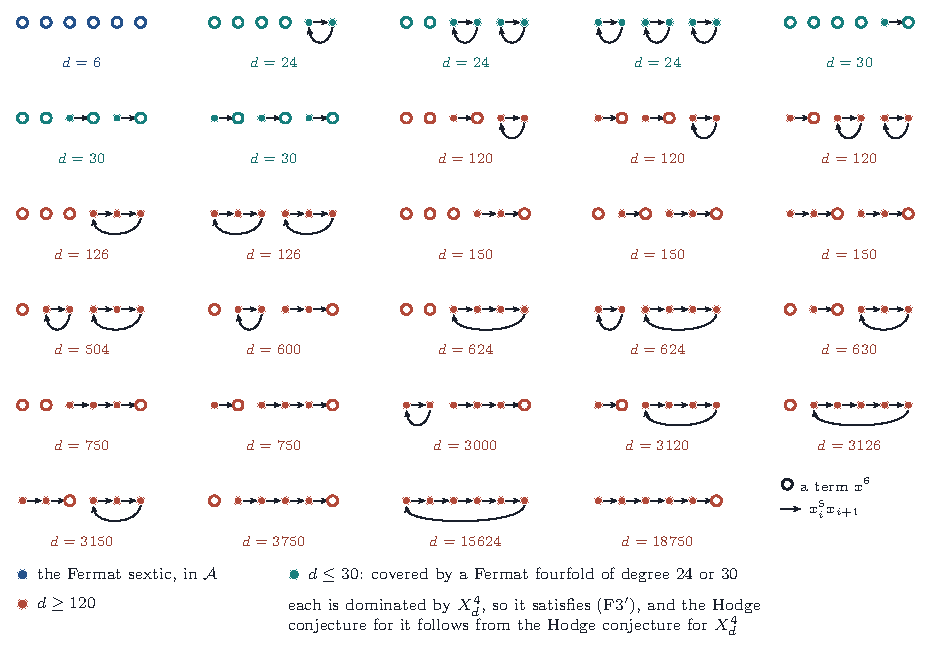
\includegraphics[width=\textwidth]{fig_delsarte}
\caption{The $29$ smooth sextic fourfolds of \Cref{prop:delsarte}(iii), up
to a renumbering of the variables. Each is drawn on its six variables: an
arrow from $x_{i}$ to $x_{j}$ is a term $x_{i}^{5}x_{j}$, and a ring is a
term $x^{6}$, so a chain is a path of arrows ending at a ring and a loop is
a cycle of arrows. Under each is the least $d$ with $dA^{-1}$ integral, the
degree of the Fermat fourfold that covers it. All of them satisfy
\textup{(F3$'$)}.}
\label{fig:delsarte}
\end{figure}

A sextic fourfold has $h^{4,0}=1$, so no hypothesis on zero-cycles or on
rationally connected fibrations reaches it (\Cref{rem:f3primesharp}), and
among the smooth sextic fourfolds only the Fermat one is covered by
\Cref{prop:aclosure}. The Delsarte sextics are finitely many
up to isomorphism, since the torus rescales the coefficients of a Delsarte
polynomial to $1$, so they are isolated points in the $426$-dimensional
moduli of smooth sextic fourfolds: \Cref{prop:delsarte} adds points, not a
family. By \Cref{prop:delsarte}(ii) the Hodge conjecture for a Delsarte
fourfold follows from that for one Fermat fourfold. For six of the sextic
shapes that Fermat fourfold has degree $24$ or $30$, inside the range claimed
in the preprint \cite{MMMV26}, so if it is correct the Hodge conjecture
itself holds on these six; for the others the degree ranges from $120$ to
$18750$, and from $120$ to $3750$ with the lattice degree of
\Cref{cor:delsarteall}, beyond every known or claimed range
\cite{Shi79b,MMMV26,Jum26}.
The monomial cover is Shioda's, and we claim no priority for it.

\Cref{prop:delsarte} uses the covering map only in degree four, where
algebraicity modulo abelian varieties descends along every dominant rational
map. In higher degrees a birational modification can add classes, so the
boundary of a compactification has to be controlled. For a hypersurface of a
torus defined by affinely independent monomials the boundary is again of the
same kind, and the whole cohomology can be traced back to Fermat varieties
of a single degree. We use toric varieties as in \cite{CLS11}: a torus $T$
with character lattice $M$ and cocharacter lattice $N$, a fan $\Sigma$ in
$N_{\RR}$ and its toric variety $Y_{\Sigma}$, and for a cone
$\tau\in\Sigma$ the orbit $O(\tau)$, whose character lattice is
$\tau^{\perp}\cap M$, and its closure $V(\tau)$, the toric variety of the
fan formed by the images of the cones containing $\tau$ in
$N_{\RR}/\RR\tau$ \cite[Chapter~3]{CLS11}; for a ray $\rho$ we write
$D_{\rho}=V(\rho)$. In what follows varieties need not be connected: a
smooth projective variety lies in $\mathcal{A}$ when each of its connected
components does, and the closure properties of \Cref{prop:f3prime}(iii) and
\Cref{prop:aclosure} hold component by component.

\begin{definition}[Simplex type]\label{def:simplextype}
Let $T$ be a torus of dimension $n$ with character lattice $M$. A Laurent
polynomial $f=\sum_{i=0}^{k}c_{i}\chi^{u_{i}}$ on $T$ is of \emph{simplex
type} if every $c_{i}$ is nonzero and $u_{0},\dots,u_{k}\in M$ are affinely
independent. Let $L'\subseteq M$ be the lattice spanned by the
$u_{i}-u_{0}$, $L$ its saturation, the set of $x\in M$ with a nonzero
multiple in $L'$, and $e(f)$ the exponent of the finite group $L/L'$; put
$V_{f}=\{f=0\}\subseteq T$. A fan $\Sigma$ in $N_{\RR}$ is \emph{adapted} to
$f$ if for every cone $\sigma\in\Sigma$ there is an index $i_{\sigma}$ with
$\langle u_{i_{\sigma}},v\rangle\le\langle u_{j},v\rangle$ for all $j$ and
all $v\in\sigma$, that is, if every cone of $\Sigma$ lies in a cone of the
normal fan of the simplex spanned by the $u_{i}$. For a cone $\tau$ of an
adapted fan let $I_{\tau}$ be the set of indices $i$ with
$\langle u_{i},v\rangle=\min_{j}\langle u_{j},v\rangle$ for every
$v\in\tau$, fix $i_{\tau}\in I_{\tau}$, and let
$f_{\tau}=\sum_{i\in I_{\tau}}c_{i}\chi^{u_{i}-u_{i_{\tau}}}$, a Laurent
polynomial of simplex type on the torus $O(\tau)$, since its exponents lie
in $\tau^{\perp}\cap M$.
\end{definition}

The compactification is Khovanskii's \cite{Kho77}; for a simplex the proof
is short, and we give it.

\begin{lemma}[The compactification]\label{lem:simplexchart}
Let $f$ be of simplex type on $T$, let $\Sigma$ be a smooth fan adapted to
$f$, and let $Z$ be the closure of $V_{f}$ in $Y_{\Sigma}$.
\begin{enumerate}[label=\textup{(\roman*)},leftmargin=2.6em,itemsep=2pt]
\item $V_{f}$ is empty if $k=0$. If $k\ge1$, it is a finite \'etale cover,
  of degree $[L:L']$, of the product of a torus of dimension $n-k$ and the
  complement of $k+1$ hyperplanes in general position in $\PP^{k-1}$; in
  particular it is smooth.
\item $Z$ is smooth, and for every $\tau\in\Sigma$, $Z\cap O(\tau)=V_{f_{\tau}}$
  and $Z$ meets $V(\tau)$ transversally: $Z\cap V(\tau)$ is empty or smooth of
  codimension $\dim\tau$ in $Z$, and it is the closure of $V_{f_{\tau}}$ in
  $V(\tau)$. So the divisors $Z\cap D_{\rho}$ of $Z$ are smooth and cross
  normally, and $Z\cap D_{\rho}$ is empty when $I_{\rho}$ has one element.
\item The fan of $V(\tau)$ is smooth and adapted to $f_{\tau}$.
\end{enumerate}
\end{lemma}

\begin{proof}
(i) If $k=0$, $f$ is a monomial and has no zero on $T$. Let $k\ge1$, choose a
complement $C$ of the saturated lattice $L$ in $M$ and a basis
$b_{k+1},\dots,b_{n}$ of $C$. The characters $u_{1}-u_{0},\dots,u_{k}-u_{0},
b_{k+1},\dots,b_{n}$ span a sublattice of index $[L:L']$ in $M$, so the map
$T\to(\CC^{\times})^{n}$ that they define is an isogeny of that degree. The
function $\chi^{-u_{0}}f$ is the pull-back of $c_{0}+c_{1}z_{1}+\dots+c_{k}
z_{k}$, so $V_{f}$ is the full preimage of the product of
$(\CC^{\times})^{n-k}$ and the set $H$ of points of $(\CC^{\times})^{k}$ with
$c_{0}+\sum_{i}c_{i}z_{i}=0$. The projective closure of this affine hyperplane is a hyperplane
$\PP^{k-1}$ of $\PP^{k}$, with homogeneous coordinates $w_{0},\dots,w_{k}$,
on which the $k+1$ linear forms $w_{i}$ satisfy the single relation
$\sum_{i}c_{i}w_{i}=0$, with every $c_{i}\ne0$; so any $k$ of them are
independent, the hyperplanes $\{w_{i}=0\}$ of $\PP^{k-1}$ are in general
position, and $H$ is their complement.

(ii) Let $\sigma\in\Sigma$, spanned by part $v_{1},\dots,v_{s}$ of a basis
$v_{1},\dots,v_{n}$ of $N$, let $w_{1},\dots,w_{n}$ be the dual basis of $M$,
and let $t_{j}=\chi^{w_{j}}$, the coordinates of
$U_{\sigma}\cong\CC^{s}\times(\CC^{\times})^{n-s}$. Put $i=i_{\sigma}$. Every
$u_{j}-u_{i}$ lies in the dual cone of $\sigma$, so
$g=\chi^{-u_{i}}f=\sum_{j}c_{j}\chi^{u_{j}-u_{i}}$ is a regular function on
$U_{\sigma}$, and $Z\cap U_{\sigma}\subseteq\{g=0\}$. A face $\tau$ of
$\sigma$ is spanned by the $v_{j}$ with $j$ in a subset $J$, and $O(\tau)$ is
the locus where exactly the $t_{j}$ with $j\in J$ vanish. A character
$\chi^{x}$ regular on $U_{\sigma}$ restricts to $O(\tau)$ as $\chi^{x}$ if
$x\in\tau^{\perp}$ and as $0$ otherwise \cite[Chapter~3]{CLS11}; since
$\langle u_{j}-u_{i},v\rangle\ge0$ on $\sigma$, $u_{j}-u_{i}\in\tau^{\perp}$
exactly when $j\in I_{\tau}$. So $h=g|_{O(\tau)}$ is
$\chi^{u_{i_{\tau}}-u_{i}}f_{\tau}$, a unit times $f_{\tau}$. Let $p\in
O(\tau)$ with $h(p)=0$ and put $a_{j}=c_{j}\chi^{u_{j}-u_{i}}(p)$ for $j\in
I_{\tau}$. The derivative of $h$ at $p$ along the one-parameter subgroup of
$O(\tau)$ given by $y$ in its cocharacter lattice is $\sum_{j}a_{j}\langle
u_{j}-u_{i},y\rangle$. If all of these vanished, then, with
$\sum_{j}a_{j}=h(p)=0$, the vector $\sum_{j}a_{j}(1,u_{j}-u_{i})$ of
$\CC\oplus(\tau^{\perp}\cap M)\otimes\CC$ would be zero, as the cocharacter
lattice of $O(\tau)$ is dual to $\tau^{\perp}\cap M$; affine independence
would give every $a_{j}=0$, which is impossible at a point of the torus
$O(\tau)$. So $dh(p)\ne0$. Hence $\{g=0\}$ is smooth at $p$ and transversal
to $O(\tau)$ and to every $\{t_{j}=0,\ j\in J'\}$ with $J'\subseteq J$, whose
tangent space at $p$ contains that of $O(\tau)$. No component of $\{g=0\}$
lies in a divisor $\{t_{j}=0\}$, since $g$ restricted to the orbit of the
ray of $v_{j}$ is a unit times a nonzero Laurent polynomial; so every
component meets $T$, where $\{g=0\}$ is $V_{f}$, and
$\{g=0\}=Z\cap U_{\sigma}$. This shows that $Z$ is smooth, that
$Z\cap O(\tau)=V_{f_{\tau}}$ and that $Z\cap V(\tau)$ is smooth of
codimension $\dim\tau$. As $Z\cap O(\tau')$ has codimension at least
$\dim\tau'$ in $Z$ for every cone $\tau'\supsetneq\tau$, no component of
$Z\cap V(\tau)$ lies in the smaller orbits, and $Z\cap V(\tau)$ is the
closure of $V_{f_{\tau}}$. If $I_{\rho}$ has one element, $f_{\rho}$ is a
nonzero constant.

(iii) The fan of $V(\tau)$ is smooth because $\Sigma$ is. Let $\sigma\supseteq
\tau$. The index $i_{\sigma}$ attains the minimum on $\sigma$, hence on
$\tau$, so $i_{\sigma}\in I_{\tau}$, and for $j\in I_{\tau}$ and $v\in\sigma$,
$\langle u_{i_{\sigma}}-u_{i_{\tau}},v\rangle\le\langle
u_{j}-u_{i_{\tau}},v\rangle$. Both sides depend only on the image of $v$ in
$N_{\RR}/\RR\tau$, because the exponents of $f_{\tau}$ lie in $\tau^{\perp}$;
so the image of $\sigma$ satisfies the condition of adaptedness for
$f_{\tau}$.
\end{proof}

\begin{lemma}[Cohomology across a toric modification]\label{lem:toricmod}
Let $f$ be of simplex type on $T$, let $\Sigma_{1}$ and $\Sigma_{0}$ be
smooth projective fans adapted to $f$, with $\Sigma_{1}$ refining
$\Sigma_{0}$, let $\varphi\colon Y_{1}=Y_{\Sigma_{1}}\to Y_{0}=Y_{\Sigma_{0}}$
be the toric morphism, and let $Z_{1}$ and $Z_{0}$ be the closures of
$V_{f}$. For each ray $\rho$ of $\Sigma_{1}$ that is not a ray of
$\Sigma_{0}$ let $E_{\rho}=Z_{1}\cap D_{\rho}$, with inclusion $i_{\rho}$.
Then the kernel of $\varphi_{*}\colon H^{k}(Z_{1},\QQ)\to H^{k}(Z_{0},\QQ)$ is
contained in $\sum_{\rho}i_{\rho*}H^{k-2}(E_{\rho},\QQ)$, and
\[
  H^{k}(Z_{1},\QQ)=\varphi^{*}H^{k}(Z_{0},\QQ)
  +\sum_{\rho}i_{\rho*}H^{k-2}(E_{\rho},\QQ).
\]
\end{lemma}

\begin{proof}
Let $W\subseteq Y_{0}$ be the union of the open sets $U_{\tau}$ with
$\tau\in\Sigma_{0}\cap\Sigma_{1}$. A cone of $\Sigma_{1}$ contained in such a
$\tau$ is a face of it, since two cones of a fan meet in a common face; so
$\varphi^{-1}(U_{\tau})=U_{\tau}$, and $\varphi$ is an isomorphism over $W$. A
cone of $\Sigma_{1}$ whose rays are all rays of $\Sigma_{0}$ lies in a cone
$\tau_{0}$ of $\Sigma_{0}$, its rays are rays of $\tau_{0}$, and $\tau_{0}$
is simplicial, so it is a face of $\tau_{0}$ and lies in $\Sigma_{0}$. Hence
$Y_{1}\smallsetminus\varphi^{-1}(W)$ is the union of the orbits of the cones
with a ray not in $\Sigma_{0}$, that is, of the divisors $D_{\rho}$ of those
rays. So $U_{1}=Z_{1}\smallsetminus\bigcup_{\rho}E_{\rho}$ is the closure of
$V_{f}$ in $\varphi^{-1}(W)$, and $\varphi$ maps it isomorphically onto
$U_{0}=Z_{0}\cap W$, with $U_{1}=Z_{1}\cap\varphi^{-1}(U_{0})$. The morphism
$Z_{1}\to Z_{0}$ is birational on each component, so $\varphi_{*}\varphi^{*}
=\id$ by the projection formula, and every class is $\varphi^{*}\varphi_{*}a$
plus a class in the kernel of $\varphi_{*}$. Let $\varphi_{*}b=0$.
Push-forward along a proper map commutes with restriction to an open set and
its preimage, so $b|_{U_{1}}=(\varphi|_{U_{1}})^{*}\bigl((\varphi_{*}b)|_{U_{0}}
\bigr)=0$. By \Cref{lem:simplexchart}(ii), $\bigcup_{\rho}E_{\rho}$ is a
divisor with normal crossings and smooth components in the smooth projective
variety $Z_{1}$, and by Deligne \cite[\S3.2]{Del71} the weight spectral
sequence of its complement $U_{1}$ degenerates at $E_{2}$; its term
$E_{2}^{0,k}$, the cokernel of the Gysin map
$\bigoplus_{\rho}H^{k-2}(E_{\rho},\QQ)\to H^{k}(Z_{1},\QQ)$, is the image of
$H^{k}(Z_{1},\QQ)$ in $H^{k}(U_{1},\QQ)$. So $b$ lies in the image of the
Gysin map.
\end{proof}

\begin{theorem}[Hypersurfaces of simplex type]\label{thm:simplextype}
Let $f$ be a Laurent polynomial of simplex type on a torus $T$ of dimension
$n$, with $e=e(f)$, let $Y$ be a projective toric variety with torus $T$,
not necessarily smooth, and let $Z$ be the closure of $V_{f}$ in $Y$.
Suppose that $Z$ is smooth.
\begin{enumerate}[label=\textup{(\roman*)},leftmargin=2.6em,itemsep=2pt]
\item $Z\in\mathcal{A}$, so \textup{(F3$'$)} holds on $Z$ in every degree.
\item If the Hodge conjecture holds for the Fermat varieties $X^{j}_{e}$
  with $j\le\dim Z$, then it holds for $Z$.
\end{enumerate}
\end{theorem}

\begin{proof}
By induction on $n$. If $k=0$, $Z$ is empty; let $k\ge1$.

\emph{The Fermat form.} With $C$ and $b_{j}$ as in the proof of
\Cref{lem:simplexchart}(i), let $\widetilde M$ be the lattice with basis
$w_{i}=(u_{i}-u_{0})/e$ for $1\le i\le k$ and $w_{j}=b_{j}$ for $k<j\le n$.
It contains $M$, since $eL\subseteq L'$ gives $L\subseteq\frac1eL'$. Let
$\widetilde T$ be the torus with character lattice $\widetilde M$,
$\widetilde N\subseteq N$ its cocharacter lattice and
$\pi\colon\widetilde T\to T$ the isogeny dual to $M\subseteq\widetilde M$.
In the coordinates $z_{i}=\chi^{w_{i}}$ of $\widetilde T$,
$\pi^{*}(\chi^{-u_{0}}f)=c_{0}+\sum_{i\le k}c_{i}z_{i}^{e}$; call it
$\widetilde f$. It is of simplex type, $V_{\widetilde f}=\pi^{-1}(V_{f})$,
and after the $z_{i}$ are rescaled it is $c_{0}(1+\sum_{i\le k}z_{i}^{e})$.

\emph{The model.} Let $\Sigma_{0}$ be the fan in $\widetilde N_{\RR}$ of
$Y_{0}=\PP^{k}\times\PP^{n-k}$, on whose torus $z_{1},\dots,z_{k}$ are the
affine coordinates of the first factor and $z_{k+1},\dots,z_{n}$ those of the
second. The closure of $V_{\widetilde f}$ in $Y_{0}$ is, after the
rescaling, $Z_{0}=X^{k-1}_{e}\times\PP^{n-k}$, since the part of the Fermat
variety in the torus is dense in it; $Z_{0}\in\mathcal{A}$ by
\Cref{prop:aclosure}(iii) and \Cref{prop:f3prime}(iii), $\PP^{n-k}$ being
the Fermat variety $X^{n-k}_{1}$. The fan $\Sigma_{0}$ is adapted to
$\widetilde f$: $\min(0,e\langle w_{1},v\rangle,\dots,e\langle
w_{k},v\rangle)$ depends only on the image of $v$ in the fan of $\PP^{k}$,
the normal fan of the standard simplex, on whose cones it is linear.

\emph{The common refinement.} Let $\Sigma_{Y}$ be the fan of $Y$, the normal
fan of a polytope $P$, as $Y$ is projective \cite[Chapter~2]{CLS11}, and
$\Sigma_{0}$ that of a polytope $Q$. The face of $P+Q$ on which a vector $v$
attains its minimum is the sum of those of $P$ and of $Q$, so the normal fan
of $P+Q$ consists of the intersections of cones of $\Sigma_{Y}$ and
$\Sigma_{0}$; it has a smooth projective refinement $\Sigma_{1}$ with
respect to $\widetilde N$ \cite[Chapter~11]{CLS11}. It is adapted to
$\widetilde f$, because $\Sigma_{0}$ is. Let
$Y_{1}=Y_{\Sigma_{1},\widetilde N}$ and $Z_{1}$ the closure of
$V_{\widetilde f}$ in it, smooth by \Cref{lem:simplexchart}(ii). The
inclusion $\widetilde N\subseteq N$ maps each cone of $\Sigma_{1}$ into a cone
of $\Sigma_{Y}$ and defines a proper toric morphism $\psi\colon Y_{1}\to Y$
extending $\pi$ \cite[Chapter~3]{CLS11}; $\psi(Z_{1})$ is closed, contains
$\pi(V_{\widetilde f})=V_{f}$ and lies in $Z$, so $\psi$ maps $Z_{1}$ onto
$Z$. The identity of $\widetilde N$ defines the toric morphism
$\varphi\colon Y_{1}\to Y_{0}$, which maps $Z_{1}$ onto $Z_{0}$ and is an
isomorphism over $V_{\widetilde f}$.

\emph{The boundary.} By \Cref{lem:simplexchart}, each $E_{\rho}=Z_{1}\cap
D_{\rho}$ is the smooth closure of $V_{\widetilde f_{\rho}}$ in the smooth
projective toric variety $D_{\rho}$ of dimension $n-1$. The exponents of
$\widetilde f_{\rho}$ are the $e(w_{i}-w_{i_{\rho}})$ with $i\in I_{\rho}$,
where $w_{0}=0$. The vectors $w_{i}-w_{i_{\rho}}$ with $i\le k$,
$i\ne i_{\rho}$, together with $w_{k+1},\dots,w_{n}$, form a basis of
$\widetilde M$, so those with $i\in I_{\rho}$ span a saturated sublattice of
$\widetilde M$, which lies in $\rho^{\perp}\cap\widetilde M$ and is
saturated there. Hence $e(\widetilde f_{\rho})=e$ if $I_{\rho}$ has at least
two elements, and $E_{\rho}$ is empty otherwise. By induction every
$E_{\rho}$ lies in $\mathcal{A}$, and it satisfies the Hodge conjecture if
the $X^{j}_{e}$ with $j\le n-2$ do.

(i) By \Cref{lem:toricmod}, $H^{*}(Z_{1},\QQ)$ is spanned by the images of
$H^{*}(Z_{0},\QQ)$ and of the $H^{*}(E_{\rho},\QQ)$ under $\varphi^{*}$ and
the $i_{\rho*}$, which are induced by algebraic cycles, the transposed
graph of $\varphi$ and the graphs of the $i_{\rho}$. So
$Z_{1}\in\mathcal{A}$ by \Cref{prop:aclosure}(v), and $Z\in\mathcal{A}$ by
\Cref{prop:f3prime}(iii), as the image of $Z_{1}$ under $\psi$.

(ii) By the K\"unneth formula every Hodge class on $X^{k-1}_{e}\times
\PP^{n-k}$ is a sum of pull-backs of Hodge classes on $X^{k-1}_{e}$
multiplied by powers of the hyperplane class, so the conjecture holds on
$Z_{0}$, as $k-1\le n-1=\dim Z$; it holds on the $E_{\rho}$ by induction.
Let $a$ be a Hodge class on $Z_{1}$. Then $\varphi_{*}a$ is a Hodge class,
hence algebraic, and so is $\varphi^{*}\varphi_{*}a$. The class
$b=a-\varphi^{*}\varphi_{*}a$ is a Hodge class in the kernel of
$\varphi_{*}$, hence in the image of the Gysin map of
\Cref{lem:toricmod}, a morphism of polarisable Hodge structures after a
Tate twist; as in the proof of \Cref{prop:f3prime}(iii) it is the image of a
Hodge class, which is algebraic, so $b$ is algebraic. So the conjecture
holds on $Z_{1}$, and it passes to $Z$ along $\psi$: for a Hodge class $x$
on $Z$, $\psi^{*}x$ is algebraic, and $\Psi_{*}\psi^{*}x=c\,x$ with $c>0$ for
the algebraic correspondence $\Psi$ of the proof of
\Cref{prop:f3prime}(iii).
\end{proof}

\begin{corollary}[Delsarte hypersurfaces of every dimension]
\label{cor:delsarteall}
Let $X_{A}\subset\PP^{r+1}$, $r\ge1$, be a smooth Delsarte hypersurface of
degree $m$ as in \Cref{prop:delsarte}, let $M=\{x\in\ZZ^{r+2}:\sum_{j}x_{j}=0\}$,
and let $e_{A}$ be the exponent of $M/M'$, where $M'$ is spanned by the
differences $a_{i}-a_{0}$ of the rows of $A$.
\begin{enumerate}[label=\textup{(\roman*)},leftmargin=2.6em,itemsep=2pt]
\item $X_{A}\in\mathcal{A}$, so \textup{(F3$'$)} holds on $X_{A}$ in every
  degree, and the Hodge conjecture holds on $X_{A}$ if it holds on the Fermat
  varieties $X^{j}_{e_{A}}$ with $j\le r$. The number $e_{A}$ divides every
  $d$ of \Cref{prop:delsarte}, and $[M:M']=|\det A|/m$.
\item The same holds, with $j\le r+1$, for the cyclic cover
  $\{y^{k}=F_{A}(x)\}$ of $\PP^{r+1}$ in the weighted projective space
  $\PP(1,\dots,1,m/k)$, for every $k$ dividing $m$, with
  $M=\{x\in\ZZ^{r+3}:\sum_{j\le r+1}x_{j}+(m/k)x_{r+2}=0\}$ and $M'$ spanned
  by the differences of the exponents of $F_{A}-y^{k}$; it is smooth
  because $X_{A}$ is.
\item For the $29$ sextic shapes of \Cref{prop:delsarte}(iii), $e_{A}$ is the
  least $d$ there, except for the chain $x_{0}^{5}x_{1}+x_{1}^{5}x_{2}+\dots
  +x_{4}^{5}x_{5}+x_{5}^{6}$ and the loop, for which it is $3125$ and $2604$
  instead of $18750$ and $15624$. For the Klein quartic
  $x^{3}y+y^{3}z+z^{3}x$ it is $7$.
\end{enumerate}
\end{corollary}

\begin{proof}
(i) On the torus of $\PP^{r+1}$, with character lattice $M$, $X_{A}$ is the
closure of $V_{f}$ for $f=\chi^{-a_{0}}F_{A}$, as in the proof of
\Cref{prop:delsarte}(i). The rows of $A$ are linearly independent and lie on
the affine hyperplane $\sum_{j}x_{j}=m$, which does not contain $0$, so they
are affinely independent, $f$ is of simplex type, $L'=M'$ has rank $r+1$ and
$L=M$; so $e(f)=e_{A}$, and \Cref{thm:simplextype} gives the first two
assertions. If $dA^{-1}$ is integral and $x\in M$, then $dx=\lambda A$ with
$\lambda=dxA^{-1}$ integral and $\sum_{i}\lambda_{i}=d\sum_{j}x_{j}/m=0$,
as $A^{-1}\mathbf{1}=\mathbf{1}/m$; so $dx=\sum_{i}\lambda_{i}(a_{i}-a_{0})
\in M'$, and $e_{A}$ divides $d$. The lattice $M'$ is the intersection of $M$
with the lattice $R$ spanned by the rows, whose image under
$x\mapsto\sum_{j}x_{j}$ is $m\ZZ$; the exact sequence $0\to M/M'\to
\ZZ^{r+2}/R\to\ZZ/m\ZZ\to0$ gives $[M:M']=|\det A|/m$.

(ii) The exponents of $F_{A}-y^{k}$ are linearly independent and lie on the
hyperplane of weighted degree $m$, so the polynomial is of simplex type on
the torus of $\PP(1,\dots,1,m/k)$, a projective toric variety whose
character lattice is the given $M$. On the affine cone, the partial
derivatives vanish together with $y^{k}-F_{A}$ only where $y=0$ and $x$ is a
singular point of the cone over $X_{A}$, that is $x=0$; so the cover is
quasi-smooth, and it misses the only singular point $(0:\dots:0:1)$ of the
weighted projective space, where $y^{k}=F_{A}(0)$ would force $y=0$. So it is
smooth. It is irreducible, $F_{A}$ being irreducible, and not contained in a
coordinate hyperplane, so it is the closure of its part in the torus, and
\Cref{thm:simplextype} applies.

(iii) The least $d$ with $dA^{-1}$ integral is the exponent of
$\ZZ^{r+2}/R$, and the map $x\mapsto\sum_{j}x_{j}$ modulo $m$ is well defined
on it because the rows sum to $m$. For a polynomial as in
\Cref{prop:delsarte}(iii) the group $\ZZ^{r+2}/R$ is the direct sum of one
group for each term. The relations of a chain are $x_{j+1}=(1-m)x_{j}$ and
$mx_{k}=0$, those of a loop are $x_{j+1}=(1-m)x_{j}$, indices modulo $k$, and
that of $x^{m}$ is $mx=0$. So each summand is cyclic, generated by the class
of its first variable, of order $N=m(m-1)^{k-1}$, $(m-1)^{k}-(-1)^{k}$ and
$m$ respectively, and the sum map sends that generator to $1$, since
$1-m\equiv1$ modulo $m$; each $N$ is divisible by $m$. The least $d$ is the
least common multiple of these orders, which gives the values of
\Cref{prop:delsarte}(iii). The group $M/M'$ is the kernel of the sum map. With
one term only, the loop or the chain in six variables, the kernel is
$m\ZZ/N\ZZ$, of exponent $N/m$, which is $15624/6=2604$ and $18750/6=3125$;
for the Klein quartic, a loop with $m=4$ and $k=3$, it is $28/4=7$. With at
least two terms, of orders $N_{1},N_{2},\dots$, the kernel contains the
differences of the generators of the first and of the $b$-th summand, of order
$\operatorname{lcm}(N_{1},N_{b})$; so its exponent is the least common multiple
of all the $N_{b}$, which is the least $d$.
\end{proof}

For the Klein quartic the construction is classical: the isogeny has kernel
of order $e_{A}^{2}/[M:M']=7$, and the Klein quartic is the quotient of the
Fermat septic curve by a group of order seven; \Cref{fig:simplextype} draws
its Newton triangle and the smooth adapted fan of the proof. For $r=4$,
\Cref{cor:delsarteall}(i) recovers \Cref{prop:delsarte}(ii), with the Fermat
degree lowered to $e_{A}$. Its content lies in dimension five and more, where
otherwise only the Fermat hypersurfaces are covered
(\Cref{prop:aclosure}(iii)), and in the cyclic covers, among them the Calabi--Yau
varieties $\{y^{2}=F_{A}(x)\}$ with $F_{A}$ of degree $2r+4$ in $r+2$
variables. Khovanskii's compactification and Shioda's cover are classical, and
we claim no priority for the two lemmas. What \Cref{thm:simplextype} adds is
that the boundary of the compactification is again of simplex type with the
same exponent $e$, so that the whole cohomology, not only its part of top
Hodge level, comes from Fermat varieties of one degree.

\begin{remark}[Quotients by diagonal automorphisms]\label{rem:delsartequotient}
Let $G\subset T$ be a finite subgroup of the torus of $\PP^{r+1}$ on which
every character $\chi^{a_{i}-a_{0}}$ is trivial, so that $G$ acts on $X_{A}$;
these $G$ are the subgroups of the group $G_{A}$ dual to $M/M'$. Then $f$
descends to a Laurent polynomial of simplex type on $T/G$, whose character
lattice $M_{G}$, the characters trivial on $G$, contains $M'$; so $L'=M'$,
$L=M_{G}$, and $e(f)$ becomes the exponent $e_{G}$ of $M_{G}/M'$, a divisor of
$e_{A}$. As $\PP^{r+1}/G$ is a projective toric variety with torus $T/G$ in
which $X_{A}/G$ is the closure of $V_{f}/G$, \Cref{thm:simplextype} applies
to every projective model $Z$ of $X_{A}/G$ that is the closure of $V_{f}/G$
in a projective toric variety with torus $T/G$ and is smooth, for instance in
one whose fan is smooth and adapted to $f$ (\Cref{lem:simplexchart}): such a
$Z$ lies in $\mathcal{A}$, and the Hodge conjecture holds on it if it holds
on the $X^{j}_{e_{G}}$ with $j\le r$. For $G=G_{A}$, $M_{G}=M'$ and $e_{G}=1$,
so the conjecture holds on $Z$. For the Fermat hypersurface of degree
$m=r+2$ and the group of diagonal automorphisms of determinant one modulo
scalars, the starting point of the mirror construction for $X_{A}$, $M'=mM$
and $M_{G}$ is the set of $x\in M$ whose coordinates are congruent modulo
$m$, so $M_{G}/M'\cong\ZZ/m$ and $e_{G}=m=e_{A}$: the quotient needs the
same Fermat varieties as $X_{A}$, and nothing is gained. For any finite
group $G$ of automorphisms of $X_{A}$, every smooth projective model $X'$ of
$X_{A}/G$ has $\Hdg^{2}(X')=\mathrm{Ab}^{2}(X')$, so \textup{(F3$'$)} holds on
it when it is a fourfold or a fivefold, by \Cref{prop:f3primedominant} and
\Cref{cor:delsarteall}(i).
\end{remark}

\begin{figure}[tbp]
\centering
  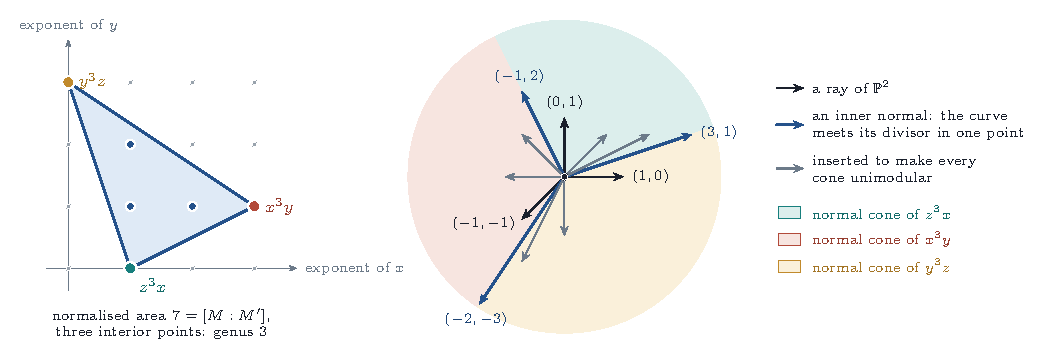
\includegraphics[width=\textwidth]{fig_simplextype}
\caption{The Klein quartic $x^{3}y+y^{3}z+z^{3}x$ in the proof of
\Cref{thm:simplextype}. Left: its Newton triangle in the lattice $M$ of the
torus of $\PP^{2}$, in the chart $z=1$, with normalised area $7=[M:M']$ and
three interior points, the genus. Right: the rays of a smooth fan adapted to
it, the three rays of $\PP^{2}$, the three inner normals of the triangle and
the six rays inserted to make every cone unimodular. The curve meets only
the three divisors of the inner normals, in one point each, the lattice
length of the edge, so its Euler number is $-7+3=-4$. With $e_{A}=7$ the
isogeny of the proof makes it the quotient of the Fermat septic by a group
of order seven.}
\label{fig:simplextype}
\end{figure}

The Fermat hypersurfaces are the complete intersections of one diagonal
hypersurface. Complete intersections of several diagonal hypersurfaces of
the same degree lie in $\mathcal{A}$ as well when their coefficients are of
Vandermonde type, because they are quotients of powers of one curve. Fix
$d\ge2$, $N\ge2$ and $1\le c\le N-1$, put $r=N-c$, and call a $c\times(N+1)$
matrix $(a_{ki})$ \emph{of Vandermonde type} if there are distinct
$\lambda_{0},\dots,\lambda_{N}\in\CC$, nonzero $\mu_{0},\dots,\mu_{N}$ and
$g\in\mathrm{GL}_{c}(\CC)$ with
$a_{ki}=\mu_{i}\sum_{l=1}^{c}g_{kl}\lambda_{i}^{l-1}$; for $c\ge2$ this says
that the columns are distinct points of a rational normal curve of degree
$c-1$ in $\PP^{c-1}$. Put $w_{i}=\prod_{l\ne i}(\lambda_{i}-\lambda_{l})^{-1}$
and
\[
  X_{d,r}(\lambda)=\Bigl\{x\in\PP^{N}:\ \sum_{i=0}^{N}w_{i}\lambda_{i}^{k}x_{i}^{d}=0,
  \ \ 0\le k\le c-1\Bigr\}.
\]
For $r=1$ this is the generalised Fermat curve of type $(d,N)$ of
Gonz\'alez-Diez, Hidalgo and Leyton \cite{GDHL09}, the Galois cover of
$\PP^{1}$ with group $H=\mu_{d}^{N+1}/\mu_{d}$, acting by
$u_{i}\mapsto h_{i}u_{i}$, branched over the $\lambda_{i}$. The characters of
$H$ are the $\chi_{a}(h)=\prod_{i}h_{i}^{a_{i}}$ with
$a\in(\ZZ/d)^{N+1}$ and $\sum_{i}a_{i}=0$; write $V_{a}\subset
H^{1}(C,\CC)$ for the eigenspace on which $h^{*}$ acts by $\chi_{a}(h)$, $[a]$
for the orbit of $a$ under $(\ZZ/d)^{\times}$, and $B_{[a]}$ for the image of
a multiple of the idempotent of $\QQ[H]$ attached to $[a]$, an abelian
subvariety of the Jacobian $J(C)$ whose first cohomology is the part
$\bigoplus_{a'\in[a]}V_{a'}$ of $H^{1}(C,\CC)$.

\begin{theorem}[Diagonal complete intersections of Vandermonde
type]\label{thm:vandermonde}
Let $X\subset\PP^{N}$ be the complete intersection of $c$ hypersurfaces
$\sum_{i}a_{ki}x_{i}^{d}=0$, $1\le k\le c$, with $(a_{ki})$ of Vandermonde
type, and let $C=X_{d,1}(\lambda)$ for the $\lambda_{i}$ of $(a_{ki})$.
\begin{enumerate}[label=\textup{(\roman*)},leftmargin=2.6em,itemsep=2pt]
\item $X$ is smooth of dimension $r$ and isomorphic to $X_{d,r}(\lambda)$,
  and $C$ is a smooth curve of genus
  $1+\tfrac12d^{N-1}\bigl((N-1)(d-1)-2\bigr)$.
\item The map
  $\Phi(u^{(1)},\dots,u^{(r)})=\bigl(\prod_{j}u^{(j)}_{i}\bigr)_{i}$ is a
  surjective morphism $C^{r}\to X_{d,r}(\lambda)$, and it induces an
  isomorphism $C^{r}/G\cong X_{d,r}(\lambda)$, where $G$ is the group of
  order $r!\,d^{N(r-1)}$ generated by the permutations of the factors and the
  $(h_{1},\dots,h_{r})\in H^{r}$ with $h_{1}\cdots h_{r}=1$.
\item $X\in\mathcal{A}$, so \textup{(F3$'$)} holds on $X$ in every degree.
\item $\dim V_{a}=\#\{i:a_{i}\ne0\}-2$ for $a\ne0$, and the Hodge conjecture
  holds on $X$ as soon as it holds on the abelian varieties $B_{[a]}$ with
  $\dim V_{a}\ge r$, which have dimension $\tfrac12|[a]|\dim V_{a}$.
\end{enumerate}
\end{theorem}

\begin{proof}
Everything rests on the Lagrange identity: interpolating a polynomial $f$
of degree at most $N$ at the $\lambda_{i}$ and comparing the coefficients of
$t^{N}$ gives $\sum_{i}w_{i}f(\lambda_{i})=0$ when $\deg f\le N-1$.%
\footnote{Lagrange interpolation writes
$f(t)=\sum_{i}f(\lambda_{i})\prod_{l\ne i}(t-\lambda_{l})/(\lambda_{i}-\lambda_{l})$
for $\deg f\le N$, and the coefficient of $t^{N}$ on the right is
$\sum_{i}w_{i}f(\lambda_{i})$. For $N=2$ and $f=1$ it says that
$\sum_{i}\prod_{l\ne i}(\lambda_{i}-\lambda_{l})^{-1}=0$ for any three
distinct numbers. The
identity says that the vector $(w_{i}\lambda_{i}^{k})_{i}$ is orthogonal to the
values of every polynomial of degree at most $N-1-k$, which is how the
equations of $X_{d,r}(\lambda)$ become the condition that the $d$-th powers of
the coordinates are the values of one polynomial of degree at most $r$.}

(i) Replacing the equations by their combinations under $g^{-1}$ and $x_{i}$
by $\nu_{i}x_{i}$ with $\nu_{i}^{d}\mu_{i}=w_{i}$ turns them into those of
$X_{d,r}(\lambda)$. Every $c\times c$ minor of $(a_{ki})$ is
$\det g\prod\mu_{i}$ times a Vandermonde determinant in distinct
$\lambda_{i}$, so any $c$ columns are independent. At a point $x$ of $X$ the
Jacobian matrix is $(d\,a_{ki}x_{i}^{d-1})$; if $S=\{i:x_{i}\ne0\}$ had at most
$c$ elements, $\sum_{i\in S}x_{i}^{d}a_{i}=0$ would be a relation between at
most $c$ columns, so $|S|>c$ and the Jacobian has rank $c$.%
\footnote{The columns of the Jacobian matrix with $i\in S$ are the columns of
$(a_{ki})$ multiplied by the nonzero numbers $d\,x_{i}^{d-1}$, and any $c$ of
the columns of $(a_{ki})$ are independent; so $c$ of them already give rank
$c$. Without the Vandermonde condition this fails: for two diagonal
quadrics in $\PP^{3}$ with proportional columns $i=0,1$, the points with
$x_{2}=x_{3}=0$ and $a_{0}x_{0}^{2}+a_{1}x_{1}^{2}=0$ are singular.} Hence $X$ is a
smooth complete intersection of dimension $r$, connected because $r\ge1$, and
the same holds for $C$. The genus follows from the Riemann--Hurwitz formula
for the cover $C\to\PP^{1}$ of degree $d^{N}$ described below, which has
$N+1$ branch points of ramification index $d$.

(ii) For $1\le k\le N-1$ let $\Lambda_{k}$ be the space of
$y\in\CC^{N+1}$ with $\sum_{i}w_{i}\lambda_{i}^{l}y_{i}=0$ for
$0\le l\le N-k-1$. The vectors $(F(\lambda_{i}))_{i}$ with $\deg F\le k$ lie
in $\Lambda_{k}$ by the identity, since $\deg t^{l}F\le N-1$; they form a space
of dimension $k+1$, since $k<N+1$; and $\Lambda_{k}$ has dimension $k+1$,
the $N-k$ equations having independent Vandermonde rows. So
$\Lambda_{k}=\{(F(\lambda_{i}))_{i}:\deg F\le k\}$, and $C$ and
$X_{d,r}(\lambda)$ are the sets of points whose $d$-th powers lie in
$\Lambda_{1}$ and in $\Lambda_{r}$. The point $u\in C$ determines
$(s:t)\in\PP^{1}$ with $u_{i}^{d}=\kappa(t-\lambda_{i}s)$ for all $i$; this is
the quotient $C\to C/H=\PP^{1}$, whose fibres are the $H$-orbits. If
$(u^{(j)}_{i})^{d}=t_{j}-\lambda_{i}s_{j}$, then
$\Phi(u)_{i}^{d}=F(\lambda_{i})$ for $F(t)=\prod_{j}(t_{j}-ts_{j})$, a nonzero
polynomial of degree at most $r<N+1$; so $\Phi(u)\in X_{d,r}(\lambda)$ and
$\Phi(u)\ne0$, and $\Phi$, given by forms of multidegree $(1,\dots,1)$ with no
common zero, is a morphism. It is $G$-invariant. Conversely, if $x\in
X_{d,r}(\lambda)$, then $(x_{i}^{d})_{i}=(F(\lambda_{i}))_{i}$ for a unique
nonzero $F$ of degree at most $r$, which factors as
$\prod_{j}(t_{j}-ts_{j})$, uniquely up to order and to rescaling the factors.
Choosing $u^{(j)}$ over $(s_{j}:t_{j})$ gives $\Phi(u)_{i}=\epsilon_{i}x_{i}$
with $\epsilon_{i}\in\mu_{d}$, and multiplying $u^{(1)}$ by
$(\epsilon_{i}^{-1})$ gives a preimage.\enlargethispage{2pt} Two preimages have the same roots, so
after a permutation $u'^{(j)}=h_{j}u^{(j)}$ with $h_{j}\in H$, and $\prod_{j}h_{j}$
acts trivially on the coordinates where $x_{i}\ne0$; where $x_{i}=0$ some
$u^{(j)}_{i}$ vanishes and $h_{j,i}$ may be changed freely, so we may take
$\prod_{j}h_{j}=1$. Hence the fibres of $\Phi$ are the $G$-orbits, $\Phi$
induces a finite bijective morphism from the normal variety $C^{r}/G$ to the
smooth variety $X_{d,r}(\lambda)$, and by Zariski's main theorem this is an
isomorphism.%
\footnote{In characteristic zero a finite morphism that is bijective on
closed points is generically \'etale of degree one, hence birational, and a
finite birational morphism onto a normal variety is an isomorphism
\cite[Chapter~III, Corollary~11.4]{Har77}. The group $G$ acts faithfully on $C^{r}$,
since $H$ is the group of deck transformations of $C\to\PP^{1}$, so
$\Phi$ has degree $|G|$.}
The order of $G$ is $r!\,|H|^{r-1}$.

(iii) $C$ is a curve, so $C^{r}\in\mathcal{A}$, and $X$ is the image of
$C^{r}$ under a surjective morphism (\Cref{prop:f3prime}(iii)).

(iv) For $a\ne0$, the forms
$t^{j}\prod_{i}(t-\lambda_{i})^{-b_{i}/d}\,dt$ with $b_{i}\in\{0,\dots,d-1\}$,
$b_{i}\equiv-a_{i}$, and $0\le j\le\sum_{i}b_{i}/d-2$, are holomorphic on $C$
and span the $\chi_{a}$-eigenspace of $H^{1,0}(C)$;%
\footnote{On the affine chart $s=1$ put $u_{i}^{d}=t-\lambda_{i}$, so that the
form is $t^{j}\prod_{i}u_{i}^{-b_{i}}\,dt$ and $h\in H$ multiplies it by
$\prod_{i}h_{i}^{-b_{i}}=\chi_{a}(h)$; it is well defined on
$H=\mu_{d}^{N+1}/\mu_{d}$ because $\sum_{i}b_{i}\equiv0$. Over $\lambda_{i}$
the cover is ramified of index $d$, with a local parameter $z$ satisfying
$z^{d}=t-\lambda_{i}$, and the form is a unit times
$z^{-b_{i}}\,d(z^{d})=d\,z^{d-1-b_{i}}\,dz$, holomorphic as $b_{i}\le d-1$.
Over $t=\infty$, with $w=1/t$ and $v^{d}=w$, it is a unit times
$v^{\,d(\sum_{i}b_{i}/d-j-2)+d-1}\,dv$, holomorphic exactly when
$j\le\sum_{i}b_{i}/d-2$, the exponent of $v$ being an integer. Forms with
different characters, or with different $j$, are independent, and their
number is
$\tfrac12\sum_{a\ne0}\bigl(\#\{i:a_{i}\ne0\}-2\bigr)
=\tfrac12\bigl((N+1)(d^{N}-d^{N-1})-2(d^{N}-1)\bigr)$, which is the genus of
(i); so they form a basis of $H^{1,0}(C)$, and each eigenspace is spanned by
the forms of its character. For $d=2$ and $N=4$ they are the five forms
$dt/\sqrt{(t-\lambda_{i_{1}})\cdots(t-\lambda_{i_{4}})}$, one for each choice
of four of the five indices, on a curve of genus five.}
its dimension
$\sum_{i}\langle-a_{i}/d\rangle-1$ and that of the $\chi_{-a}$-eigenspace add up
to $\#\{i:a_{i}\ne0\}-2$, and $H^{1}(C)^{H}=H^{1}(\PP^{1})=0$. The group $H$
acts trivially on $H^{0}(C)$ and $H^{2}(C)$, so a tensor in
$H^{r}(C^{r})=\bigoplus\bigotimes_{j}H^{k_{j}}(C)$ invariant under the
$(h_{j})$ with $\prod_{j}h_{j}=1$ has all its factors in $H^{1}$, with one
character, or none: taking $h$ in one factor and $h^{-1}$ in another shows
that two factors carry the same character, and a factor in $H^{0}$ or
$H^{2}$ carries the trivial one. Taking the invariants of the permutations,
\[
  H^{r}(C^{r},\CC)^{G}=\CC\,\eta\;\oplus\;\bigoplus_{a\ne0}\textstyle\bigwedge^{r}V_{a},
\]
with $\eta$ the symmetrised product of $r/2$ classes of points when $r$ is
even and $\eta=0$ otherwise, and $W_{[a]}=\bigoplus_{a'\in[a]}\bigwedge^{r}V_{a'}$
is a sub-Hodge structure defined over $\QQ$, zero unless $\dim V_{a}\ge r$.
Let $\psi\colon C\to B_{[a]}$ be an Abel--Jacobi map followed by the
projection, so that $\psi^{*}$ maps $H^{1}(B_{[a]},\QQ)$ isomorphically onto
the $[a]$-part of $H^{1}(C,\QQ)$, and let $\sigma\colon C^{r}\to B_{[a]}$ be
$\sum_{j}\psi\circ\mathrm{pr}_{j}$. Then
$\sigma^{*}(\alpha_{1}\wedge\dots\wedge\alpha_{r})=\prod_{k}\sum_{j}
\mathrm{pr}_{j}^{*}\psi^{*}\alpha_{k}$, whose component in
$H^{1}(C)^{\otimes r}$ is the alternating sum of the
$\psi^{*}\alpha_{1}\otimes\dots\otimes\psi^{*}\alpha_{r}$. The K\"unneth
projectors of a curve are algebraic,%
\footnote{For a curve $C$ with a point $o$ they are $\pi_{0}=[o\times C]$,
$\pi_{2}=[C\times o]$ and $\pi_{1}=[\Delta_{C}]-\pi_{0}-\pi_{2}$, and
$\pi_{1}^{\otimes r}$ is their exterior product on $C^{r}\times C^{r}$. The
average $e_{G}=|G|^{-1}\sum_{g\in G}[\Gamma_{g}]$ of the graphs of the
elements of $G$ acts on $H^{*}(C^{r})$ as the projector onto the invariants,
and $\Phi^{*}$ identifies $H^{*}(X_{d,r}(\lambda),\QQ)$ with
$H^{*}(C^{r},\QQ)^{G}$.} and so is the average $e_{G}$ over $G$,
so $e_{G}\circ\pi_{1}^{\otimes r}\circ\sigma^{*}$ is induced by an algebraic
cycle on $B_{[a]}\times C^{r}$, and it maps $H^{r}(B_{[a]},\QQ)$ onto
$W_{[a]}$: the alternating tensors in the $[a]$-part are the image of
$\pi_{1}^{\otimes r}\circ\sigma^{*}$, and $e_{G}$ keeps those of one
character. A surjective morphism of polarisable Hodge structures maps Hodge
classes onto Hodge classes,%
\footnote{The category of polarisable rational Hodge structures is semisimple,
so the kernel of a surjective morphism $f\colon V\to W$ has a complement
$V'$, a sub-Hodge structure that $f$ maps isomorphically onto $W$; a Hodge
class of $W$ is then the image of a Hodge class of $V'$.} so the Hodge classes of $W_{[a]}$ are algebraic
when those of $B_{[a]}$ are. Now let $x$ be a Hodge class of degree $r$ on
$X=X_{d,r}(\lambda)$, the other degrees being multiples of powers of the
hyperplane class by the Lefschetz hyperplane theorem. Then $\Phi^{*}x$ is a
$G$-invariant Hodge class, its components in the $W_{[a]}$ and along $\eta$
are Hodge classes, being cut out by the algebraic projectors attached to
the action of $H^{r}$, and they are algebraic; so $\Phi^{*}x$ is algebraic,
and so is $x=\Phi_{*}\Phi^{*}x/|G|$.\enlargethispage{2pt} Finally $\dim B_{[a]}$ is half of
$\sum_{a'\in[a]}\dim V_{a'}=|[a]|\dim V_{a}$.
\end{proof}

\begin{corollary}[Two diagonal hypersurfaces]\label{cor:twodiagonal}
\leavevmode
\begin{enumerate}[label=\textup{(\roman*)},leftmargin=2.6em,itemsep=2pt]
\item Every smooth complete intersection of two diagonal hypersurfaces
  $\sum_{i}a_{i}x_{i}^{d}=\sum_{i}b_{i}x_{i}^{d}=0$ of the same degree in
  $\PP^{N}$ is of Vandermonde type, so it lies in $\mathcal{A}$ and
  satisfies \textup{(F3$'$)} in every degree.
\item Let $d\in\{3,4,6\}$ and $N\le6$, or $d=2$ and $N\le12$. Then the
  Hodge conjecture holds on every complete intersection of Vandermonde type
  in $\PP^{N}$ of $N-r$ diagonal hypersurfaces of degree $d$. In particular
  it holds on every smooth complete intersection of two diagonal
  hypersurfaces of degree $3$, $4$ or $6$ in $\PP^{6}$.
\item For $d\in\{3,4,6\}$ and $N=6$, each orbit $[a]$ of order at least
  three with six nonzero coordinates and $\sum_{i}\langle a_{i}/d\rangle=3$ makes $B_{[a]}$ an
  abelian fourfold of Weil type for $K=\QQ(\zeta_{d})$, and $W_{[a]}$ is its
  space of Weil classes. On each of these fourfolds $X$ the Weil classes of
  the $70$, $490$ and $6125$ such orbits, for $d=3,4,6$, give Hodge classes of
  degree four outside $\QQ h^{2}$, so the Hodge classes of $X$ form a space of
  dimension at least $141$, $981$ and $12251$, whereas the divisor classes of
  $X$ are the multiples of $h$.
\end{enumerate}
\end{corollary}

\begin{proof}
(i) If two columns $(a_{i},b_{i})$ and $(a_{j},b_{j})$ were proportional,
or one of them zero, $X$ would contain a point supported on $\{i,j\}$, or
the coordinate point $e_{i}$, at which the Jacobian has rank at most one;
so the $N+1$ columns are distinct points of $\PP^{1}$. Sending a point of
$\PP^{1}$ outside them to infinity writes them as
$\mu_{i}(1,\lambda_{i})$ with distinct $\lambda_{i}$, which is the
Vandermonde form for $c=2$, and \Cref{thm:vandermonde}(iii) applies.
(ii) For $d\in\{2,3,4,6\}$ every $a$ has order $1$, $2$, $3$, $4$ or $6$, so
$|[a]|\le2$, with $|[a]|=1$ for the $a$ of order two, whose $V_{a}$ is real,
so that $\dim B_{[a]}\le\dim V_{a}\le N-1$. When $d=2$ every $a\ne0$ has
order two and an even number of nonzero coordinates, at most $12$ when
$N\le12$, so $\dim B_{[a]}=\tfrac12\dim V_{a}\le5$. So every $B_{[a]}$ has
dimension at most five,%
\footnote{Both bounds are sharp: for $d=3$ and $N=7$ a character with eight
nonzero coordinates has $\dim V_{a}=6$ and $|[a]|=2$, so $\dim B_{[a]}=6$;
for $d=2$ and $N=13$ a character with fourteen nonzero coordinates has
$\dim B_{[a]}=6$.} and the Hodge
conjecture holds on abelian varieties of dimension at most five
\cite{Mar25a,Mar25b,MZ99}; \Cref{thm:vandermonde}(iv) gives the conclusion,
and (i) the last statement.
(iii) For such $a$ the eigenspaces $V_{a}$ and $V_{-a}$ have dimension four
and contain two-dimensional parts of type $(1,0)$, so $K$ acts on
$H^{1,0}(B_{[a]})$ with multiplicities $(2,2)$ and $B_{[a]}$, of dimension
four, is of Weil type; $\bigwedge^{4}V_{a}$ and $\bigwedge^{4}V_{-a}$ are its
Weil lines, of type $(2,2)$ for every $\lambda$, and they lie in
$H^{4}(C^{4})^{G}=\Phi^{*}H^{4}(X)$. The zero coordinate of $a$ is one of
seven, and the other six $a_{i}\in\{1,\dots,d-1\}$ add up to $3d$, which
they do in $20$, $141$ and $1751$ ways for $d=3,4,6$, the coefficients of
$x^{3d-6}$ in $(1+x+\dots+x^{d-2})^{6}$; removing the character of order two
with every $a_{i}=d/2$ leaves $20$, $140$ and $1750$, and $(\ZZ/d)^{\times}=
\{\pm1\}$ pairs them off, since $-a$ again has coordinate sum $3d$; this
gives $7\cdot20/2=70$, $7\cdot140/2=490$ and $7\cdot1750/2=6125$ orbits.
Distinct orbits give independent classes, and the hyperplane class
lies in the part of the trivial character, which gives the bounds; the
Picard group of a complete intersection of dimension at least three is
generated by $h$.
\end{proof}

\Cref{fig:vandermonde} draws the construction. For $c=1$ the theorem is \Cref{prop:aclosure}(iii) again,
by a different route, and for $r=1$ it restates the definition of $C$.

\begin{figure}[tbp]
\centering
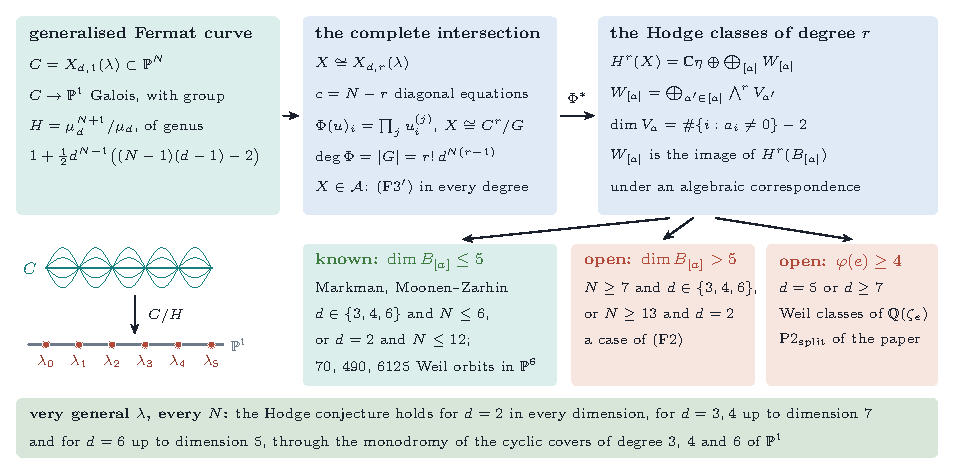
\includegraphics[width=\textwidth]{fig_vandermonde}
\caption{\Cref{thm:vandermonde} and \Cref{cor:twodiagonal}. Left: the
generalised Fermat curve $C$ over $\PP^{1}$, its sheets meeting over the
branch points $\lambda_{0},\dots,\lambda_{N}$ (five sheets stand for the
$d^{N}$ of the cover). Top: $C$, the complete intersection
$X\cong C^{r}/G$ with the map $\Phi$ of degree $|G|$, and the decomposition
of $H^{r}(X)$ through $\Phi^{*}$. Bottom: where the Hodge conjecture for $X$
stands at an arbitrary configuration, according to the abelian varieties
$B_{[a]}$ that carry its Hodge classes: known when they have dimension at
most five, which happens for $d\in\{3,4,6\}$ and $N\le6$ and for $d=2$ and
$N\le12$, and open when they are larger, a case of (F2), or carry Weil
classes of $\QQ(\zeta_{e})$ with $\varphi(e)\ge4$, the case
$\mathrm{P2}_{\mathrm{split}}$ of the paper. Foot: the very general
configuration, \Cref{thm:vgvandermonde}.}
\label{fig:vandermonde}
\end{figure}

At a very general configuration the abelian varieties $B_{[a]}$ carry only
the Hodge classes that the monodromy of the curves allows, and the
conjecture can then be decided in every dimension for $d=2$, up to dimension
seven for $d=3$ and $d=4$, and up to dimension five for $d=6$. Write $U\subset\CC^{N+1}$ for the space of
$(N+1)$-tuples of distinct numbers. The varieties $X_{d,r}(\lambda)$ with
$\lambda\in U$ form a smooth projective family over $U$, and so do the
curves $C$ and the maps $\Phi$, with $H$ acting on the family of curves.

\begin{lemma}[Hodge classes of a very general member]\label{lem:vgmonodromy}
Let $\mathbb{V}$ be a polarised variation of $\ZZ$-Hodge structure of weight
$2p$ on a smooth connected quasi-projective variety $S$, and let
$\Pi=\pi_{1}(S,s)$ act on $\mathbb{V}_{s}$. If $s$ lies outside a countable
union of proper Zariski closed subsets of $S$, the space $\Hdg(\mathbb{V}_{s})$
of rational classes of type $(p,p)$ is stable under $\Pi$, and a subgroup of
finite index of $\Pi$ fixes it pointwise.
\end{lemma}

\begin{proof}
The locus of Hodge classes has countably many components
(\Cref{def:hodgelocus}, \Cref{lem:hodgeanalytic}), and the image in $S$ of
each is Zariski closed (\Cref{thm:cdk}); let $s$ avoid the images that are
not all of $S$. For $\alpha\in\Hdg(\mathbb{V}_{s})$ the component through
$(s,\alpha)$ maps onto $S$, locally biholomorphically onto its image, so the
flat section $\tilde\alpha$ through $\alpha$ on the universal cover $\tilde S$
is of type $(p,p)$ on a nonempty open set. The set where it is of type
$(p,p)$ is a closed analytic subset of the connected manifold $\tilde S$, so it
is all of $\tilde S$, and every transport of $\alpha$ along a loop at $s$ is a
Hodge class at $s$. The group $\Pi$ therefore preserves
$\Hdg(\mathbb{V}_{s})$, the lattice $\mathbb{V}_{s,\ZZ}\cap\Hdg(\mathbb{V}_{s})$
and the flat form $\tilde Q$ of the proof of \Cref{lem:boundednorm}, which is
positive definite on the real classes of type $(p,p)$; so it acts on
$\Hdg(\mathbb{V}_{s})$ through a finite group, whose kernel is the subgroup
of the statement.
\end{proof}

For the characters of order three, four and six the monodromy of the
curves $D_{a}$ is determined by induction on the number of branch points. The
step lets two branch points collide, and a lemma on two copies of $\SL$ of a
hyperplane closes it. The base has four branch points, two of them with
opposite exponents, whose full twist is a transvection
(\Cref{fig:cyclicmerge}).

\begin{setupenv}[Cyclic covers]\label{setup:cyclic}
Let $m\in\{3,4,6\}$, $\zeta=e^{2\pi i/m}$ and $K=\QQ(\zeta)$, and let
$a=(a_{1},\dots,a_{k})$ with $a_{i}\in\ZZ/m$ nonzero, $\sum_{i}a_{i}=0$ and
$\gcd(m,a_{1},\dots,a_{k})=1$, so that $a$ has order $m$. For $\lambda$ in
the space $\mathrm{Conf}_{k}$ of $k$-tuples of distinct complex numbers let
$D_{a}$ be the cyclic cover $y^{m}=\prod_{i}(t-\lambda_{i})^{a_{i}}$ of
$\PP^{1}$, with representatives $0<a_{i}<m$; it is unramified over
$\infty$. Let $V_{a}\subset H^{1}(D_{a},\CC)$ be the eigenspace of the deck
group on which $H^{1,0}$ is spanned by the forms
$t^{j}\prod_{i}(t-\lambda_{i})^{-b_{i}/m}\,dt$, where $0<b_{i}<m$, $b_{i}\equiv
-a_{i}$ and $0\le j\le\sum_{i}b_{i}/m-2$ \cite[\S2]{DM86}, and put
$n=\dim V_{a}$,
$p=\dim V_{a}^{1,0}=\sum_{i}b_{i}/m-1$ and $q=n-p$. Let $\Gamma_{a}\subset
\GL(V_{a})$ be the image of the pure braid group
$P_{k}=\pi_{1}(\mathrm{Conf}_{k})$ and $G_{a}^{0}$ the identity component of
its Zariski closure.
\end{setupenv}

\begin{lemma}[A model of the monodromy]\label{lem:foxmodel}
Let $F_{k}$ be the free group on loops $x_{1},\dots,x_{k}$ around
$\lambda_{1},\dots,\lambda_{k}$, put $t_{i}=\zeta^{a_{i}}$, let
$\partial\colon K^{k}\to K$ map $e_{i}$ to $t_{i}-1$, and let
$E_{a}=\ker\partial/K\ell$, where $\ell=\sum_{i}t_{1}\cdots t_{i-1}e_{i}$. A pure
braid $\beta$ acts on $F_{k}$ by Artin's automorphism and on $K^{k}$ by
$v\mapsto vJ_{\beta}$, where $J_{\beta}$ is the matrix of Fox derivatives
$\partial\beta(x_{i})/\partial x_{j}$ evaluated at $x_{j}\mapsto t_{j}$. This
action preserves $\ker\partial$ and fixes $\ell$, and the representation of
$P_{k}$ on $E_{a}$, of dimension $k-2$, is isomorphic to $V_{a}$, to its dual
or to its complex conjugate. So $n=k-2$, and $G_{a}^{0}\supseteq\SL(V_{a})$ if
and only if the identity component of the Zariski closure of the image of
$P_{k}$ in $\GL(E_{a})$ contains $\SL(E_{a})$.
\end{lemma}

\begin{proof}
Fox's formula $\sum_{j}(\partial w/\partial x_{j})(x_{j}-1)=w-1$ \cite{Fox53},
evaluated at $x_{j}\mapsto t_{j}$, shows that the vector
$\sum_{j}(\partial w/\partial x_{j})(t)\,e_{j}$ of a word $w$ with $t(w)=1$ lies
in $\ker\partial$. It is the class of the lift of the loop $w$ in the summand
of $H_{1}(D_{a}^{\circ},K)$ on which the deck group acts through
$x_{i}\mapsto t_{i}$, where $D_{a}^{\circ}$ is the unramified part of the
cover, and that summand is $H_{1}(F_{k},K_{t})=\ker\partial$, computed from the
free resolution of length one of the augmentation ideal of a free group.%
\footnote{By Shapiro's lemma $H_{1}(D_{a}^{\circ},K)=H_{1}(F_{k},K[\mu_{m}])$,
and its summand for the character $x_{i}\mapsto t_{i}$ is $H_{1}(F_{k},K_{t})$.
The augmentation ideal of $\ZZ[F_{k}]$ is free on the $x_{i}-1$, so
$H_{1}(F_{k},K_{t})$ is the kernel of $\bigoplus_{i}Ke_{i}\to K$,
$e_{i}\mapsto t_{i}-1$, the chain $e_{i}$ standing for the loop $x_{i}$ and a word
$w$ for $\sum_{j}(\partial w/\partial x_{j})(t)e_{j}$.} Filling in the points
over $\lambda_{i}$ adds no relation: the loop around such a point lifts
$x_{i}^{e}$, $e$ the order of $t_{i}$, whose vector
$(1+t_{i}+\dots+t_{i}^{e-1})e_{i}$ is zero. Filling in the $m$ points over
$\infty$, where the cover is unramified, kills the lift of $x_{1}\cdots
x_{k}$, whose vector is $\ell\ne0$. So $E_{a}$ is the summand of
$H_{1}(D_{a},K)$ for the character $x_{i}\mapsto t_{i}$, of dimension $k-2$. A
pure braid fixes $x_{1}\cdots x_{k}$ and maps each $x_{i}$ to a conjugate of
itself, so it preserves $t$, and the chain rule for Fox derivatives makes
$\beta\mapsto J_{\beta}$ the action of $P_{k}$ on this summand.%
\footnote{Artin's automorphism of the half twist $\sigma_{i}$ of the $i$-th
and $(i+1)$-st points is $x_{i}\mapsto x_{i}x_{i+1}x_{i}^{-1}$,
$x_{i+1}\mapsto x_{i}$, the other generators being fixed; $P_{k}$ is generated
by the full twists $A_{st}=\sigma_{t-1}\cdots\sigma_{s+1}\sigma_{s}^{2}
\sigma_{s+1}^{-1}\cdots\sigma_{t-1}^{-1}$. For a pure braid the chain rule
reads $J_{\beta\beta'}=J_{\beta'}J_{\beta}$ or $J_{\beta}J_{\beta'}$, according
to the convention for composing braids, with no twist of the coefficients,
since $t\circ\beta=t$.} Poincar\'e duality and the choice of the generator
of the deck group identify it with $V_{a}$, its dual or its conjugate, and
the automorphisms $g\mapsto{}^{t}g^{-1}$ and $g\mapsto\bar g$ of $\GL$ preserve
$\SL$.
\end{proof}

\begin{lemma}[Collision of two branch points]\label{lem:cabling}
In \Cref{lem:foxmodel} suppose that $a_{1}+a_{2}\ne0$, and let
$a'=(a_{1}+a_{2},a_{3},\dots,a_{k})$. Let $I=(1-t_{2})e_{1}-(1-t_{1})e_{2}$,
the cycle of a disc around $\lambda_{1}$ and $\lambda_{2}$, and let
$Y\subset E_{a}$ be the image of the cycles outside that disc, the vectors of
$\ker\partial$ with $v_{2}=t_{1}v_{1}$. Then $E_{a}=Y\oplus KI$, and
$\iota(v_{1},v_{3},\dots,v_{k})=(v_{1},t_{1}v_{1},v_{3},\dots,v_{k})$ induces an
isomorphism $E_{a'}\to Y$. If $\beta\in P_{k}$ is obtained from
$\beta'\in P_{k-1}$ by doubling its first strand, then $\beta$ preserves $Y$
and $KI$, acts on $Y$ as $\beta'$ acts on $E_{a'}$, and multiplies $I$ by a
power of $\zeta$.
\end{lemma}

\begin{proof}
The vectors of $Y$ have $(v_{1},v_{2})$ proportional to $(1,t_{1})$, and
$(1-t_{2},t_{1}-1)$ is proportional to $(1,t_{1})$ only if $t_{1}t_{2}=1$; so
$I\notin Y$. The map $\iota$ carries the kernel of $\partial'$, where
$\partial'(e_{1})=t_{1}t_{2}-1$, onto the cycles outside the disc, because
$v_{1}(t_{1}t_{2}-1)=v_{1}(t_{1}-1)+t_{1}v_{1}(t_{2}-1)$, and it carries the
vector $\ell'$ of $a'$ to $\ell$; as $\dim E_{a'}+1=\dim E_{a}$, both
assertions about $Y$ follow. The doubled braid moves a disc containing
$\lambda_{1},\lambda_{2}$ rigidly. Its automorphism therefore maps
$x_{1}\mapsto wx_{1}w^{-1}$, $x_{2}\mapsto wx_{2}w^{-1}$ and $x_{j}\mapsto
u_{j}$ for $j\ge3$, where $y\mapsto w'yw'^{-1}$, $x_{j}\mapsto u_{j}'$ is the
automorphism of $\beta'$ on the free group on $y,x_{3},\dots,x_{k}$, and
$w,u_{j}$ are $w',u_{j}'$ with $y$ replaced by $x_{1}x_{2}$. For such a word
$u$ the chain rule gives $\partial u/\partial x_{1}=\partial u/\partial y$
and $\partial u/\partial x_{2}=(\partial u/\partial y)\,x_{1}$, which at $t$ is
the relation $v_{2}=t_{1}v_{1}$; together with
$\partial(wx_{i}w^{-1})/\partial x_{j}=(1-t_{i})\,\partial w/\partial
x_{j}+t(w)\delta_{ij}$ at $t$, this shows that the rows of $J_{\beta}$ for
$j\ge3$, and the first row plus $t_{1}$ times the second, are the images under
$\iota$ of the rows of $J_{\beta'}$; this is the equivariance of $\iota$. The
same formula gives $IJ_{\beta}=(1-t_{2})\bigl((1-t_{1})\partial w+t(w)e_{1}\bigr)
-(1-t_{1})\bigl((1-t_{2})\partial w+t(w)e_{2}\bigr)=t(w)I$, and $t(w)$ is a
power of $\zeta$.
\end{proof}

\begin{lemma}[Two hyperplanes]\label{lem:hyperplanes}
Let $E=Y\oplus L$ be a complex vector space with $\dim Y\ge2$ and
$\dim L=1$, let $S\subset\SL(E)$ be the subgroup acting on $Y$ through
$\SL(Y)$ and trivially on $L$, and let $\gamma\in\GL(E)$ satisfy
$\gamma L\ne L$ and $\gamma Y\ne Y$. Then the group $T$ generated by $S$ and
$\gamma S\gamma^{-1}$ acts irreducibly on $E$. If $\dim Y\ge3$, then
$T=\SL(E)$. If $\dim Y=2$, every connected semisimple subgroup of $\SL(E)$
that contains $T$ is $\SL(E)$.
\end{lemma}

\begin{proof}
The group $T$ is connected. As a representation of $S$, $E$ is
the sum of the irreducible nontrivial $Y$ and the trivial $L$, so its
$S$-stable subspaces are $0$, $L$, $Y$ and $E$, and those of
$\gamma S\gamma^{-1}$ are $0$, $\gamma L$, $\gamma Y$ and $E$; by the
hypotheses and the dimensions only $0$ and $E$ are in both lists, and $T$ is
irreducible.

Let $\dim Y\ge3$. As a representation of $\mathfrak{sl}(Y)$,
\[
  \mathfrak{sl}(E)=\mathfrak{sl}(Y)\oplus\mathrm{Hom}(L,Y)\oplus
  \mathrm{Hom}(Y,L)\oplus\CC z,
\]
$z$ acting by $1$ on $Y$ and by $-\dim Y$ on $L$, and the four summands, the
adjoint representation, $Y$, $Y^{*}$ and the trivial one, are pairwise
non-isomorphic since $\dim Y\ge3$. The Lie algebra $\mathfrak{t}$ of $T$
contains $\mathfrak{sl}(Y)$ and is stable under it, so it is
$\mathfrak{sl}(Y)$ plus some of the other three summands. Without
$\mathrm{Hom}(L,Y)$ it preserves $L$, and without $\mathrm{Hom}(Y,L)$ it
preserves $Y$; both are excluded by irreducibility. The bracket of a nonzero
map $L\to Y$ with a map $Y\to L$ not vanishing on its image has a nonzero
component along $z$, so $\mathfrak{t}=\mathfrak{sl}(E)$ and $T=\SL(E)$.

Let $\dim Y=2$ and let $G\supseteq T$ be connected and semisimple. Then $E$
is a faithful irreducible representation of dimension $3$ of the Lie algebra
$\mathfrak{g}$ of $G$. An irreducible representation of a product of simple
Lie algebras is a tensor product of irreducible representations of the
factors, and $3$ is prime, so $\mathfrak{g}$ is simple. It lies in
$\mathfrak{sl}(E)$, of dimension $8$ and rank $2$, and the simple Lie
algebras of rank at most $2$ are $\mathfrak{sl}_{2}$, $\mathfrak{sl}_{3}$,
$\mathfrak{so}_{5}$ and $\mathfrak{g}_{2}$, of dimensions $3$, $8$, $10$ and
$14$. If $\mathfrak{g}\cong\mathfrak{sl}_{2}$, then $\mathfrak{g}$ equals the
Lie algebra of $S$, both being of dimension $3$, so $G=S$, which preserves
$L$, against the irreducibility of $T$. Hence $\mathfrak{g}=\mathfrak{sl}(E)$
and $G=\SL(E)$.
\end{proof}

\begin{lemma}[Merging two branch points]\label{lem:merge}
Let $m$ and $a$ be as in \Cref{setup:cyclic}, with $k\ge6$ and $p,q\ge1$.
Then there are $i\ne j$ with $a_{i}+a_{j}\ne0$ such that the vector $a'$
obtained by replacing $a_{i}$ and $a_{j}$ by $a_{i}+a_{j}$ has order $m$, and
its numbers $p'$ and $q'$ are at least $1$.
\end{lemma}

\begin{proof}
Put $f_{i}=b_{i}/m\in[1/m,1-1/m]$, so that $p+1=\sum_{i}f_{i}$ and
$q+1=\sum_{i}(1-f_{i})$. Merging $a_{i}$ and $a_{j}$ keeps $p$ and lowers $q$
by one if $f_{i}+f_{j}<1$, and lowers $p$ by one and keeps $q$ if
$f_{i}+f_{j}>1$. Since $a_{i}+a_{j}=-\sum_{l\ne i,j}a_{l}$, the order of $a'$ is
that of the subgroup generated by the $a_{l}$ with $l\ne i,j$, the rest of
$a$. Replacing $a$ by $-a$ exchanges $p$ and $q$, so we may assume $q\ge p$,
hence $q\ge2$ as $p+q=k-2\ge4$; if $p\ge2$, every merge keeps $p',q'\ge1$
and only the order matters.

\emph{The order.} For $m=3$ two equal coordinates exist, their sum is not
$0$, and any nonzero rest generates $\ZZ/3$. For $m=4$ the number of odd
coordinates is even and positive; if it is at least $4$, merge two equal odd
ones, and if it is $2$, merge an odd one with one of the at least four
coordinates equal to $2$. For $m=6$ the rest generates $\ZZ/6$ exactly when
it contains an odd coordinate and one prime to $3$. The odd coordinates
are even in number and the coordinates prime to $3$ have sum divisible by
$3$, so each kind occurs at least twice. If exactly two coordinates are
odd, the at least four others lie in $\{2,4\}$; merge two equal ones among
them. If exactly two are prime to $3$, the others equal $3$; merge a $3$
with one of the two. Otherwise each kind occurs at least three times, and
any two coordinates with nonzero sum can be merged; they exist, since
pairwise sums $0$ would force every coordinate to be $3$.

\emph{The case $p=1$.} Then $\sum_{i}b_{i}=2m$. Some $b_{i}$ equals $1$,
since otherwise $\sum_{i}b_{i}\ge2k\ge12\ge2m$, with equality only if $m=6$
and every coordinate is $4$, when $a$ has order three. Keep such a coordinate,
$a_{i}=-1$, which generates $\ZZ/m$. The other $k-1\ge5$ coordinates have
$b$-sum $2m-1$, so the two smallest values of $b$ among them add up to at most
$2(2m-1)/5<m$; merge these two coordinates. Their sum is not $0$, $p'=p=1$,
$q'=q-1=k-4\ge2$, and the rest contains $a_{i}$, so $a'$ has order $m$.
\end{proof}

\begin{lemma}[Five branch points]\label{lem:mergefive}
Let $m$ and $a$ be as in \Cref{setup:cyclic}, with $k=5$ and $p,q\ge1$. Then
$a_{i}+a_{j}=0$ for some $i\ne j$, and the other three coordinates can be
labelled $x,y,z$ so that $x+y\ne0$ and $a'=(x+y,z,a_{i},a_{j})$ has order $m$
and $p'=q'=1$.
\end{lemma}

\begin{proof}
Replacing $a$ by $-a$ we may assume $p=1$, so that $\sum_{l}b_{l}=2m$ with
five terms in $[1,m-1]$; and $a_{i}+a_{j}=0$ means $b_{i}+b_{j}=m$. For $m=3$
the terms lie in $\{1,2\}$ and exactly one is $2$; take it and a $1$. For
$m=4$, take a $3$ and a $1$ if both occur. If no term is $3$, the terms lie in
$\{1,2\}$ and at least three are $2$, which gives $2+2$; if no term is $1$,
they lie in $\{2,3\}$ and add up to at least $10$, which is impossible. For
$m=6$ suppose that no two terms add up to $6$. Then at most one term is $3$,
and neither $1$ and $5$ nor $2$ and $4$ both occur. Terms in $\{1,2,3\}$ with
at most one $3$ add up to at most $11$, and terms in $\{3,4,5\}$ to at least
$19$. Terms in $\{1,3,4\}$, respectively $\{2,3,5\}$, cannot add up to $12$,
since the number $y$ of terms $4$, respectively $5$, would satisfy
$3y\in\{7,5\}$, respectively $3y\in\{2,1\}$. This proves the first assertion.

The other three coordinates add up to $0$ and have $b$-sum $m$, so any two of
them, $x$ and $y$, have $x+y=-z\ne0$ and $b$-sum less than $m$; merging them
keeps $p'=1$, so $q'=1$, and $a'$ contains $c=a_{i}$ and $a_{j}=-c$. The order
of $a'$ is that of the subgroup generated by $z$ and $c$. If $c$ generates
$\ZZ/m$, any choice of $z$ will do. Otherwise $c$ is even, or $m=6$ and $c=3$.
As $a$ has order $m$, one of $x,y,z$ is then odd, respectively prime to $3$,
and we take it as $z$; then $z$ and $c$ generate $\ZZ/m$.
\end{proof}

\begin{proposition}[Monodromy of cyclic covers]\label{prop:cyclicmonodromy}
In \Cref{setup:cyclic}, if $p=0$ or $q=0$ then $\Gamma_{a}$ is finite, and if
$n\ge3$ and $p,q\ge1$ then $G_{a}^{0}\supseteq\SL(V_{a})$.
\end{proposition}

\begin{proof}
If $pq=0$, the polarisation is definite on $V_{a}$ up to sign, and
$\Gamma_{a}$ preserves it and the $\ZZ[\zeta]$-lattice spanned by
$H^{1}(D_{a},\ZZ)$; a discrete subgroup of a compact group is finite. Assume
$p,q\ge1$ and use the model of \Cref{lem:foxmodel}. Three facts are used
throughout. If $u\in\Gamma_{a}$ is unipotent, the Zariski closure of its
powers is the group $\exp(\tau\log u)$, so $\log u$ lies in the Lie algebra
of $G_{a}^{0}$. The group $\Gamma_{a}$ normalises $G_{a}^{0}$. And $G_{a}^{0}$
is semisimple: by Andr\'e's theorem \cite[Theorem~1]{And92} the identity
component of the Zariski closure of the monodromy group of
$H^{1}(D_{a},\QQ)$ is a normal subgroup of the derived group of the
Mumford--Tate group of a very general fibre, hence semisimple, and
$G_{a}^{0}$ is its image in $\GL(V_{a})$, the monodromy commuting with the
deck group.

\emph{Four points.} Let $k=4$, so $n=2$, and suppose that two coordinates
of $a$ are opposite; relabel them $a_{1}$ and $a_{2}$, so that $t_{1}t_{2}=1$.
The full twist $A_{12}$ maps $x_{i}\mapsto wx_{i}w^{-1}$ for $i=1,2$, with
$w=x_{1}x_{2}$, and fixes $x_{3},x_{4}$. As $t(w)=1$, the formula for
$\partial(wx_{i}w^{-1})/\partial x_{j}$ in the proof of \Cref{lem:cabling}
gives $vJ_{A_{12}}=v+\varphi(v)\,\delta$, with $\delta=e_{1}+t_{1}e_{2}$ and
$\varphi(v)=(1-t_{1})v_{1}+(1-t_{2})v_{2}$, which equals
$\sum_{j\ge3}(t_{j}-1)v_{j}$ on $\ker\partial$. Here $\delta\in\ker\partial$,
$\varphi(\delta)=0$, $\varphi(\ell)=t_{1}\cdots t_{k}-t_{1}t_{2}=0$, the
vector $\delta$ is not a multiple of $\ell$, whose third coordinate is
$t_{1}t_{2}=1$, and $\varphi\bigl((t_{3}-1)e_{1}-(t_{1}-1)e_{3}\bigr)
=-(t_{1}-1)(t_{3}-1)\ne0$. So $A_{12}$ acts on $E_{a}$ as a unipotent
$u\ne1$, and $G_{a}^{0}$ is a connected semisimple subgroup of
$\SL(E_{a})\cong\SL_{2}$ containing $\exp(\tau\log u)$. The connected
subgroups of $\SL_{2}$ of dimension one or two are solvable, so
$G_{a}^{0}=\SL(E_{a})$.

\emph{The induction.} Let $n\ge3$. If $n=3$, \Cref{lem:mergefive} gives,
after a relabelling, a vector $a'=(a_{1}+a_{2},a_{3},a_{4},a_{5})$ of order $m$
with $a_{1}+a_{2}\ne0$, $p'=q'=1$ and two opposite coordinates, so the
identity component of the Zariski closure of the monodromy of $E_{a'}$ is
$\SL(E_{a'})$ by the case of four points. If $n\ge4$, \Cref{lem:merge} and
a relabelling give $a_{1}+a_{2}\ne0$ and $a'=(a_{1}+a_{2},a_{3},\dots,a_{k})$
of order $m$ with $p',q'\ge1$, and by induction on $n$ that identity
component contains $\SL(E_{a'})$. Let $H$ be the identity component of the
Zariski closure of the doubled braids of \Cref{lem:cabling}. Then
$H\subseteq G_{a}^{0}$, $H$ preserves $Y$ and $KI$ and acts trivially on
$KI$, where the doubled braids act through a finite group, and its image in
$\GL(Y)$ is the identity component of the Zariski closure of the monodromy of
$E_{a'}$, which contains $\SL(Y)$. So $G_{a}^{0}$ contains the group $S$ of
\Cref{lem:hyperplanes} for $E_{a}=Y\oplus KI$. Let $\gamma=A_{23}$, the full
twist of the second and third points; its automorphism fixes $x_{1}$ and
maps $x_{2}\mapsto x_{2}x_{3}x_{2}x_{3}^{-1}x_{2}^{-1}$ and $x_{3}\mapsto
x_{2}x_{3}x_{2}^{-1}$. Then $\gamma(I)=I+(1-t_{1})t_{2}I_{23}$ with
$I_{23}=(1-t_{3})e_{2}-(1-t_{2})e_{3}$, and $\gamma(KI)\ne KI$, since $I$,
$I_{23}$ and $\ell$ are independent, $\ell$ having a nonzero fourth
coordinate. The functional $v\mapsto v_{2}-t_{1}v_{1}$ vanishes on $\ell$ and
cuts out $Y$, and at $\gamma(v)$ for $v\in Y$ it equals
$(t_{3}-1)(t_{1}t_{2}v_{1}-v_{3})$, which is nonzero for the cycle
$(1-t_{4})e_{3}-(1-t_{3})e_{4}$ of $Y$; so $\gamma Y\ne Y$. As $\gamma$
normalises $G_{a}^{0}$, this group contains $S$ and $\gamma S\gamma^{-1}$,
and \Cref{lem:hyperplanes}, with $\dim Y=n-1$, gives
$G_{a}^{0}=\SL(E_{a})$: for $n\ge4$ directly, and for $n=3$ because
$G_{a}^{0}$ is connected and semisimple.
\end{proof}

For $m=3$ the proposition also follows from the $\ell$-adic theorem of
Achter and Pries \cite[Corollary~3.10]{AP07}, which identifies the monodromy
of trielliptic curves with a special unitary group.

\begin{lemma}[The discriminant of the new part]\label{lem:newdisc}
In \Cref{setup:cyclic} let $n$ be even with $p=q=n/2$, let
$L=H^{1}(D_{a},\ZZ)$ with the cup product $Q$, and let
$L_{a}=L\cap(V_{a}\oplus\overline{V_{a}})$. Then $L_{a}$ is a free
$\ZZ[\zeta]$-module of rank $n$, the $K$-hermitian form $H$ with
$Q=\tfrac12\Tr_{K/\QQ}(\delta^{-1}H)$ on it, $\delta=\sqrt{-1}$ for $m=4$ and
$\delta=\sqrt{-3}$ otherwise (\Cref{lem:hermform}), has signature
$(n/2,n/2)$, and the class of $(-1)^{n/2}\det H$ in
$\QQ^{\times}/\Nm(K^{\times})$ is trivial for $m=3$ and $m=4$; for $m=6$ it is
trivial if and only if the number of $i$ with $a_{i}=3$ is even.
\end{lemma}

\begin{proof}
The deck transformation $g$ is an isometry of the unimodular lattice $L$, so
its eigenspaces for eigenvalues $\mu,\nu$ are orthogonal unless $\mu\nu=1$.
Hence $L_{a}$, the part for the primitive $m$-th roots of unity, and the
part $L^{\mathrm{old}}$ for the other eigenvalues are orthogonal primitive
sublattices, each the orthogonal complement of the other, and
$|\det(L_{a})|=|\det(L^{\mathrm{old}})|$, which is $1$ for $m=3$, when
$L^{\mathrm{old}}=0$.%
\footnote{If $M\subset L$ is primitive and $L$ is unimodular, restriction
$L\to M^{\vee}$ is onto with kernel $M^{\perp}$, so $L/(M\oplus M^{\perp})\cong
M^{\vee}/M$, and likewise $\cong(M^{\perp})^{\vee}/M^{\perp}$; the order of
$M^{\vee}/M$ is $|\det M|$.} For a quotient map $\pi\colon D_{a}\to D'$ of
prime degree $e$ that is ramified, $\pi^{*}H^{1}(D',\ZZ)$ is primitive in $L$
and the cup product on it is $e$ times that of $D'$.%
\footnote{A loop in $D'$ avoiding the branch points, composed with a loop
around a branch point, whose monodromy generates the group of order $e$,
lifts to a closed loop with the same image in $H_{1}(D',\ZZ)$; so
$\pi_{*}\colon H_{1}(D_{a},\ZZ)\to H_{1}(D',\ZZ)$ is onto, and its transpose
$\pi^{*}$ is a split injection. The factor $e$ is $\pi_{*}\pi^{*}=e$.} For
$m=4$, $L^{\mathrm{old}}=\pi^{*}H^{1}(D',\ZZ)$ for the quotient $D'$ by $g^{2}$,
ramified over the $\lambda_{i}$ with $a_{i}$ odd, so
$|\det L^{\mathrm{old}}|=2^{2g'}$, $g'$ the genus of $D'$. For $m=6$, the
quotients $D_{2}$ by $g^{2}$ and $D_{3}$ by $g^{3}$ are ramified over the
$\lambda_{i}$ with $3\nmid a_{i}$ and with $a_{i}$ odd, which exist since $a$
has order six, and $L^{\mathrm{old}}$ contains $A\oplus B$ with
$A=\pi_{2}^{*}H^{1}(D_{2},\ZZ)$ and $B=\pi_{3}^{*}H^{1}(D_{3},\ZZ)$, of determinants
$3^{2g_{2}}$ and $2^{2g_{3}}$; the quotient $L^{\mathrm{old}}/(A\oplus B)$ embeds in
$A^{\vee}/A$ and in $B^{\vee}/B$, of coprime orders, so $L^{\mathrm{old}}=A\oplus B$
and $|\det L^{\mathrm{old}}|=3^{2g_{2}}2^{2g_{3}}$.

On $L_{a}$ the deck transformation satisfies the cyclotomic equation of $\zeta$,
so $L_{a}$ is a torsion-free module over the principal ideal domain
$\ZZ[\zeta]$, free of rank $n$; the signature of $H$ is $(p,q)$
(\Cref{rem:twosignatures}). The determinant of the trace form of a hermitian
lattice gives $|\det(L_{a})|=|d_{K}|^{n}\Nm(\tfrac{1}{2\delta})^{n}(\det H)^{2}$,
that is $(\det H)^{2}$ for $K=\QQ(i)$ and $(\det H)^{2}/4^{n}$ for
$K=\QQ(\sqrt{-3})$.%
\footnote{For a free $\cO_{K}$-module with hermitian Gram matrix $M$ and
$c\in K^{\times}$, the $\ZZ$-bilinear form $\Tr_{K/\QQ}(c\,v^{T}M\bar w)$ has
determinant of absolute value $|d_{K}|^{n}\Nm(c)^{n}(\det M)^{2}$, where
$d_{K}$ is the discriminant of $K$: for $n=1$ this is the discriminant of the
trace form of $\cO_{K}$ scaled by $\Nm(cM)$. Changing the basis by
$P\in\GL_{n}(K)$ multiplies both sides by $\Nm_{K/\QQ}(\det P)^{2}$, and a
basis in which $M$ is diagonal makes the form an orthogonal sum of forms of
rank one. Here $d_{K}=-4$ and $\Nm(\tfrac{1}{2i})=\tfrac14$, or $d_{K}=-3$ and
$\Nm(\tfrac{1}{2\sqrt{-3}})=\tfrac1{12}$.}
Hence $(-1)^{n/2}\det H$ equals $2^{n}$ for $m=3$, $2^{g'}$ for $m=4$ and
$2^{n+g_{3}}3^{g_{2}}$ for $m=6$, the sign being that of a form of signature
$(n/2,n/2)$. For $m=3$ this is $\Nm(2^{n/2})$, and for $m=4$ a norm as
$2=\Nm(1+i)$. For $m=6$, $3=\Nm(\sqrt{-3})$ and $4=\Nm(2)$
are norms and $2$ is not, since $x^{2}+xy+y^{2}$ is even only when $x$ and $y$
are, so that every norm has even $2$-adic valuation; so the class is trivial
exactly when $g_{3}$ is even. By the Riemann--Hurwitz formula $D_{3}$, the
triple cover $y^{3}=\prod_{i}(t-\lambda_{i})^{a_{i}}$ branched over the $i$
with $3\nmid a_{i}$, has genus $k-c_{3}-2=n-c_{3}$, where $c_{3}$ is the number
of $i$ with $a_{i}=3$; as $n$ is even, this is the assertion.
\end{proof}

\begin{figure}[tbp]
\centering
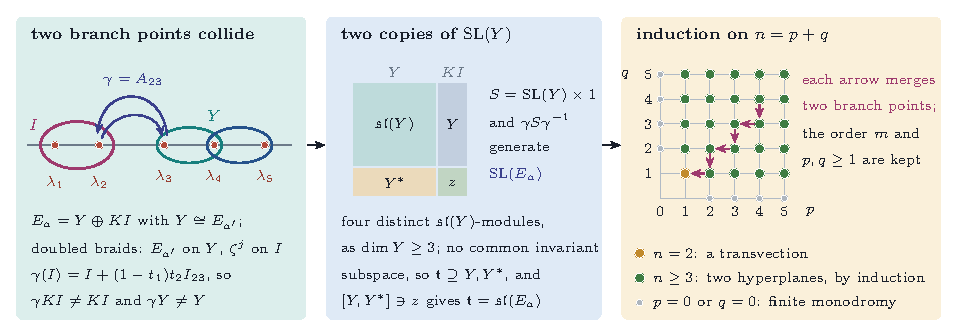
\includegraphics[width=\textwidth]{fig_cyclicmerge}
\caption{The proof of \Cref{prop:cyclicmonodromy}. Left: two branch points
$\lambda_{1},\lambda_{2}$ collide inside a disc (\Cref{lem:cabling}); the
cycles outside the disc form the hyperplane $Y\cong E_{a'}$, the cycle $I$
of the disc spans the complementary line, and the twist $\gamma$ of the
second and third points moves both. Middle: the two copies of $\SL(Y)$ of
\Cref{lem:hyperplanes}, which generate $\SL(E_{a})$ when $\dim Y\ge3$. Right: the induction on
$n=k-2$, each merge lowering $p$ or $q$ by one (\Cref{lem:merge},
\Cref{lem:mergefive}), down to $n=2$, where the full twist of two points
with opposite exponents is a transvection.}
\label{fig:cyclicmerge}
\end{figure}

\begin{theorem}[Very general diagonal complete
intersections]\label{thm:vgvandermonde}
Keep the notation of \Cref{thm:vandermonde}, let $r\ge2$ be even, and let
$\lambda\in U$ lie outside a countable union of proper Zariski closed
subsets of $U$. For a Hodge class $x$ of degree $r$ on $X=X_{d,r}(\lambda)$,
write $x_{[a]}$ for the component of $\Phi^{*}x$ in $W_{[a]}$.
\begin{enumerate}[label=\textup{(\roman*)},leftmargin=2.6em,itemsep=2pt]
\item If $a$ has order two, then $x_{[a]}$ is a rational multiple of the
  image of $\theta_{a}^{r/2}$, where $\theta_{a}$ is the class of a
  polarisation of $B_{[a]}$, under the correspondence of the proof of
  \Cref{thm:vandermonde}(iv); in particular $x_{[a]}$ is algebraic.
\item If $a$ has order $m\in\{3,4,6\}$ and $x_{[a]}\ne0$, then $\dim V_{a}=r$
  and $\dim V_{a}^{1,0}=r/2$. In that case $B_{[a]}$ is an abelian variety of
  dimension $r$ of Weil type for $\QQ(\zeta_{m})$, and $W_{[a]}$ is the image
  of its space of Weil classes. Its discriminant is trivial for $m=3,4$, and
  for $m=6$ exactly when an even number of the coordinates of $a$ equal
  $d/2$.
\item The Hodge conjecture holds on $X_{d,r}(\lambda)$ for every $N$ when
  $d=2$, when $d\in\{3,4\}$ and $r\le6$, and when $d=6$ and $r\le4$. For
  $d=6$ and $r=6$ the Hodge classes are algebraic modulo the spaces
  $W_{[a]}$ of the characters of order six of (ii) with an odd number of
  coordinates $3$, which are spaces of Weil classes of abelian sixfolds of
  non-split Weil type for $\QQ(\sqrt{-3})$ and occur for every $N$. For
  $d\in\{2,3,4,6\}$ the Hodge classes of degree $r$ form a space of dimension
  \[
    1+\binom{N+1}{r+2}T_{d}(r+2)+\epsilon_{d}\sum_{j\ge r/2+2}\binom{N+1}{2j},
  \]
  where $T_{d}(k)$ is the number of $(s_{1},\dots,s_{k})\in\{1,\dots,d-1\}^{k}$
  with $\sum_{i}s_{i}=dk/2$, and $\epsilon_{d}$ is $1$ for $d$ even and $0$ for
  $d$ odd; thus $T_{2}(k)=1$, $T_{3}(k)=\binom{k}{k/2}$, $T_{4}(6)=141$ and
  $T_{6}(6)=1751$.
\end{enumerate}
\end{theorem}

For odd $r$ there is nothing to prove, since every Hodge class of $X$ is
then a multiple of a power of the hyperplane class. So the theorem gives the
Hodge conjecture for the very general complete intersection of Vandermonde
type of diagonal quadrics in every dimension, of diagonal cubics or quartics
up to dimension seven, and of diagonal sextics up to dimension five, in
every $\PP^{N}$.

\begin{proof}
Apply \Cref{lem:vgmonodromy} to $H^{r}(X_{d,r}(\lambda),\ZZ)$ over $U$,
polarised by the hyperplane class, and let $\Pi'\subset\pi_{1}(U,\lambda)$ be
the subgroup of finite index that fixes the Hodge classes. The monodromy
commutes with $H$ and with $\Phi^{*}$, so $\Pi'$ fixes $x_{[a]}$ and each of
its parts in the spaces $\bigwedge^{r}V_{a'}$. Let $m$ be the order of $a$,
take representatives $0\le a_{i}<d$, and put $a_{i}'=ma_{i}/d$. The function
$y=\prod_{i}u_{i}^{a_{i}}$ is invariant under the kernel of $\chi_{a}$ and
satisfies $y^{m}=\prod_{i}(t-\lambda_{i})^{a_{i}'}$, so the quotient of $C$ by
that kernel is the cyclic cover $D_{a}$ of $\PP^{1}$ of degree $m$ given by
this equation, and pull-back identifies $H^{1}(D_{a},\QQ)$ with the part
$\bigoplus_{j\ne0}V_{ja}$ of $H^{1}(C,\QQ)$, compatibly with the monodromy.
The image $B_{[a]}$ is isogenous to the abelian subvariety of $J(D_{a})$
whose first cohomology is $\bigoplus_{j\in(\ZZ/m)^{\times}}V_{ja}$, all of
$J(D_{a})$ for $m\le3$, its polarisation being a rational multiple of the
restriction of the principal one, since pull-back along a map of degree $e$
multiplies the cup product by $e$.

(i) For $m=2$, $D_{a}$ is the hyperelliptic curve
$y^{2}=\prod_{i\in S}(t-\lambda_{i})$ over the support $S$ of $a$, of genus
$g=|S|/2-1$, and $H^{1}(D_{a},\QQ)=V_{a}$. Move the base point so that the
$\lambda_{i}$ with $i\in S$ are real and consecutive, $\lambda_{s_{1}}<\dots<
\lambda_{s_{2g+2}}$, the others lying away from the segment they span. The
loop in which $\lambda_{s_{k}}$ and $\lambda_{s_{k+1}}$ turn once around each
other, inside a disc that contains no other $\lambda_{i}$, makes $D_{a}$
acquire a node with vanishing cycle $c_{k}$, the lift of the segment
$[\lambda_{s_{k}},\lambda_{s_{k+1}}]$, and acts by the square of the
Picard--Lefschetz transvection,
$T_{k}^{2}(z)=z+2\langle z,c_{k}\rangle c_{k}$ up to orientation
\cite[Chapter~3]{Voi03}.%
\footnote{Near the collision the curve is $y^{2}=(t-\lambda_{s_{k}})
(t-\lambda_{s_{k+1}})\,v$ with $v$ a unit, analytically $y^{2}=t^{2}-\epsilon$
with $\epsilon$ a multiple of $(\lambda_{s_{k+1}}-\lambda_{s_{k}})^{2}$; one
turn of the two points around each other is two turns of $\epsilon$ around
$0$, and one turn
of $\epsilon$ acts by the Dehn twist along the vanishing cycle, whose action on
$H_{1}$ is the transvection $T_{k}$.} The classes $c_{1},\dots,c_{2g}$ satisfy
$\langle c_{k},c_{k+1}\rangle=\pm1$ and $\langle c_{k},c_{l}\rangle=0$ for
$|k-l|\ge2$, so their intersection matrix has determinant $1$ and they form a
basis of $H_{1}(D_{a},\QQ)$; they are the distinguished basis of type $A$ of
\cite{ACa79}. Some power $T_{k}^{2e}$ with $e\ge1$ lies in the image of
$\Pi'$; it is unipotent, so the Zariski closure of that image contains the
one-parameter group $\exp(\tau N_{k})$, $N_{k}(z)=\langle z,c_{k}\rangle c_{k}$,
and its Lie algebra contains $N_{1},\dots,N_{2g}$. These generate the Lie
algebra $\mathfrak{sp}(V_{a})$.%
\footnote{Identify $\mathfrak{sp}(V)$ with $\mathrm{Sym}^{2}V$, the product $uv$
acting by $z\mapsto\langle z,u\rangle v+\langle z,v\rangle u$, so that
$N_{k}=\tfrac12c_{k}^{2}$ and
$[uv,wz]=\langle u,w\rangle vz+\langle u,z\rangle vw+\langle v,w\rangle uz
+\langle v,z\rangle uw$ up to an overall sign. Then
$[c_{k}^{2},c_{k+1}^{2}]=\pm4c_{k}c_{k+1}$, and if all products
$c_{i}c_{j}$ with $i,j\le k$ lie in the generated algebra, so do the
$c_{i}c_{k+1}=\pm\tfrac12[c_{i}c_{k},c_{k+1}^{2}]$ for $i<k$, because
$c_{k+1}$ meets only $c_{k}$ among $c_{1},\dots,c_{k}$. By induction every
$c_{i}c_{j}$ lies in it, and these span $\mathrm{Sym}^{2}V$.} So the Zariski
closure contains $\Sp(V_{a})$, whose invariants in
$\bigwedge^{r}V_{a}$ are the multiples of $\omega_{a}^{r/2}$, $\omega_{a}$ the
polarisation form \cite[Theorem~17.5]{FH91}.%
\footnote{The exterior algebra of $V$ is a representation of $\Sp(V)$
and of the $\mathfrak{sl}_{2}$ spanned by $\omega\wedge{}$ and its adjoint,
and $\bigwedge^{r}V=\bigoplus_{j}\omega^{j}\wedge P^{r-2j}$, where $P^{k}$, the
kernel of the contraction with $\omega$ in degree $k\le g$, is irreducible
and nontrivial for $k\ge1$, so the invariants are the multiples of
$\omega^{r/2}$, for $r$ even.} The correspondence of the proof of
\Cref{thm:vandermonde}(iv) maps $H^{r}(B_{[a]},\QQ)=\bigwedge^{r}H^{1}(B_{[a]},
\QQ)$ isomorphically and equivariantly onto $\bigwedge^{r}V_{a}$; the class
$\theta_{a}$ goes to an invariant nondegenerate form, a nonzero multiple of
$\omega_{a}$, and $\theta_{a}^{r/2}$ to a nonzero multiple of
$\omega_{a}^{r/2}$, which is algebraic.

(ii) For $m\in\{3,4,6\}$, $D_{a}$ is the cyclic cover of \Cref{setup:cyclic}
for the exponents $a_{i}'\in\{1,\dots,m-1\}$ on the support $S$ of $a$, and
$V_{a}$ is its eigenspace, of dimension $n=|S|-2$ (\Cref{lem:foxmodel}). The
map from $U$ to $\mathrm{Conf}_{|S|}$ that forgets the $\lambda_{i}$ outside
$S$ is a fibration with connected fibres, so it is onto on fundamental groups,
and $\Pi'$ maps onto a subgroup of finite index of $P_{|S|}$; the Zariski
closure of its image in $\GL(V_{a})$ therefore contains $G_{a}^{0}$. If
$n\le2$, then $\bigwedge^{r}V_{a}$ is zero unless $r=n=2$. If $V_{a}^{1,0}$ or
$V_{a}^{0,1}$ is zero, then $\bigwedge^{r}V_{a}$ has type $(r,0)$ or $(0,r)$
and contains no class of type $(r/2,r/2)$. Otherwise $n\ge3$, and
\Cref{prop:cyclicmonodromy} gives $G_{a}^{0}\supseteq\SL(V_{a})$, whose
invariants in $\bigwedge^{r}V_{a}$ vanish for $0<r<n$. In every case
$x_{[a]}\ne0$ forces $r=n$, and then $\bigwedge^{r}V_{a}$ is a line of type
$(p_{a},r-p_{a})$ with $p_{a}=\dim V_{a}^{1,0}$, which contains a class of type
$(r/2,r/2)$ only if $p_{a}=r/2$. The field $\QQ(\zeta_{m})$ then acts on
$B_{[a]}$, of dimension $|[a]|\dim V_{a}/2=r$, with multiplicities
$(r/2,r/2)$ on the tangent space and compatibly with the polarisation, the
automorphism of $D_{a}$ preserving the cup product; so $B_{[a]}$ is of Weil
type (\Cref{def:weiltype}), and
$W_{[a]}=\bigwedge^{r}V_{a}\oplus\bigwedge^{r}V_{-a}$ is the image of
$\bigwedge^{r}_{\QQ(\zeta_{m})}H^{1}(B_{[a]},\QQ)$, its space of Weil classes.
Its discriminant (\Cref{def:disc}) is that of the lattice $L_{a}$ of
\Cref{lem:newdisc}: the isogeny with the abelian subvariety of $J(D_{a})$
whose first cohomology is $L_{a}\otimes\QQ$ scales the polarisation by a
rational number and $\det H$ by its $r$-th power, a norm. The coordinates of
$a$ equal to $d/2$ are those with $a_{i}'=3$ when $m=6$, and
\Cref{lem:newdisc} gives the assertion.

(iii) Let $x$ be a Hodge class of degree $r$. The component of $\Phi^{*}x$
along $\eta$ is algebraic. For $d\in\{2,3,4,6\}$ every $a\ne0$ has order $2$,
$3$, $4$ or $6$, and by (i) and (ii) the components $x_{[a]}$ are images of
powers of polarisations or of Weil classes of abelian $r$-folds of Weil type
for $\QQ(\sqrt{-3})$ or $\QQ(i)$. These are algebraic for $r=2$ by the theorem
of Lefschetz, for $r=4$ by Markman's theorem on abelian fourfolds of Weil
type, and for $r=6$ by Markman's theorem on abelian sixfolds of split Weil
type \cite{Mar25a,Mar25b} when the discriminant is trivial: always for
$d=3,4$, and for $d=6$ except along the characters of order six with an odd
number of coordinates $3$. So $\Phi^{*}x$ is
algebraic in the cases stated, and so is $x=\Phi_{*}\Phi^{*}x/|G|$. For the
dimension, the classes found are Hodge at every $\lambda$, and by (i) and (ii)
there are no others. Each character of order two with $|S|\ge r+2$ gives one
class, the image of $\theta_{a}^{r/2}$, nonzero since $r\le\dim V_{a}$. A
character of order at least three gives a class only if $|S|=r+2$ and
$\dim V_{a}^{1,0}=\sum_{i\in S}(d-a_{i})/d-1=r/2$, that is
$\sum_{i}a_{i}=d(r+2)/2$ with representatives $0\le a_{i}<d$, and then exactly
one, in $\bigwedge^{r}V_{a}$. The characters with $|S|=r+2$ whose coordinates
on $S$ average $d/2$ are counted by $T_{d}(r+2)$; for $d$ even they include
the one of order two with all coordinates $d/2$, and the characters of order
two with $|S|\ge r+4$ give the last sum.
\end{proof}

\begin{figure}[tbp]
\centering
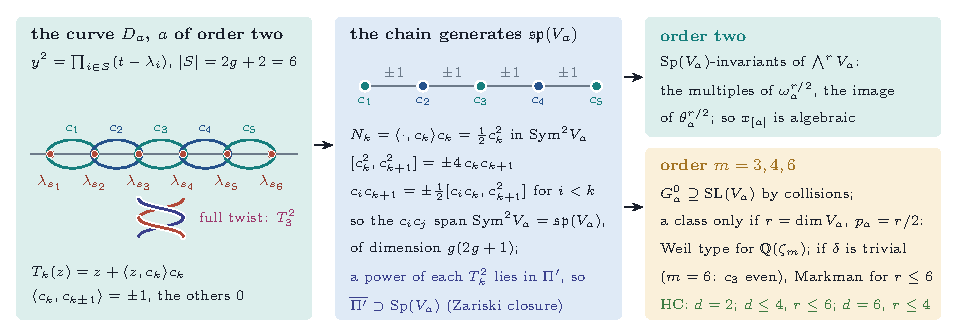
\includegraphics[width=\textwidth]{fig_vgmonodromy}
\caption{The proof of \Cref{thm:vgvandermonde}. Left: the hyperelliptic
curve $D_{a}$ of a character of order two, drawn over the six points of its
support for $g=2$, with the chain of vanishing cycles $c_{1},\dots,c_{5}$;
a full twist of two neighbouring branch points, drawn as a braid, acts by
the square of the transvection $T_{k}$. Middle: the chain as a graph, and the
induction in $\mathrm{Sym}^{2}V_{a}$ by which the logarithms $N_{k}$ generate
$\mathfrak{sp}(V_{a})$. Right: what the monodromy leaves of the Hodge
classes, the powers of the polarisation for characters of order two, and
for characters of order three, four and six the Weil classes of an abelian
variety of Weil type for $\QQ(\sqrt{-3})$ or $\QQ(i)$.}
\label{fig:vgmonodromy}
\end{figure}

\Cref{fig:vgmonodromy} draws the steps of the proof. The dimensions of (iii)
never exceed $h^{r/2,r/2}(X)$, and they equal it for a quadric, for
the Fermat hypersurfaces (for cubics $7$, $21$ and $71$ in dimensions $2$, $4$
and $6$, for quartics $142$ and $1108$ in dimensions $4$ and $6$, for sextics
$1752$ in dimension $4$) and for two quadrics in $\PP^{N}$ with $N$ even
($N+2$), where every class of type $(r/2,r/2)$ is algebraic. For two cubics
in $\PP^{6}$ the very general member has $141$ Hodge classes of degree four
against $h^{2,2}=267$, and for three quartics in $\PP^{7}$ it has $3950$
against $h^{2,2}=29872$ (\Cref{fig:vgcounts}). \Cref{fig:vgscope} shows, for each degree $d$ and dimension $r$,
what is known for the very general member.

\begin{figure}[tbp]
\centering
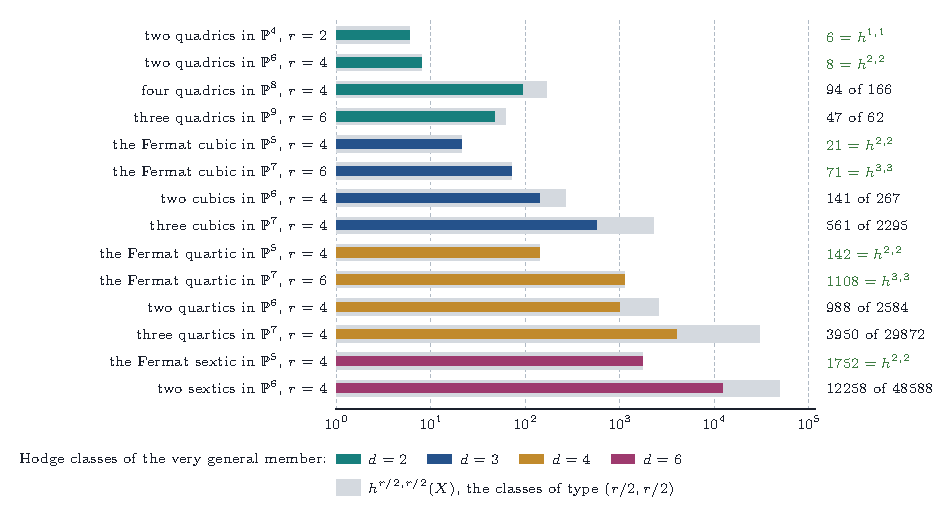
\includegraphics[width=\textwidth]{fig_vgcounts}
\caption{The dimension of the space of Hodge classes of degree $r$ on the
very general member, from \Cref{thm:vgvandermonde}(iii), against the Hodge
number $h^{r/2,r/2}$, on a logarithmic scale. Where the two agree, the
space $H^{r/2,r/2}$ is spanned by Hodge classes at every configuration;
elsewhere the very general member has fewer Hodge classes, and the members
with more lie over a countable union of proper closed subsets of the space
of configurations.}
\label{fig:vgcounts}
\end{figure}

\begin{figure}[tbp]
\centering
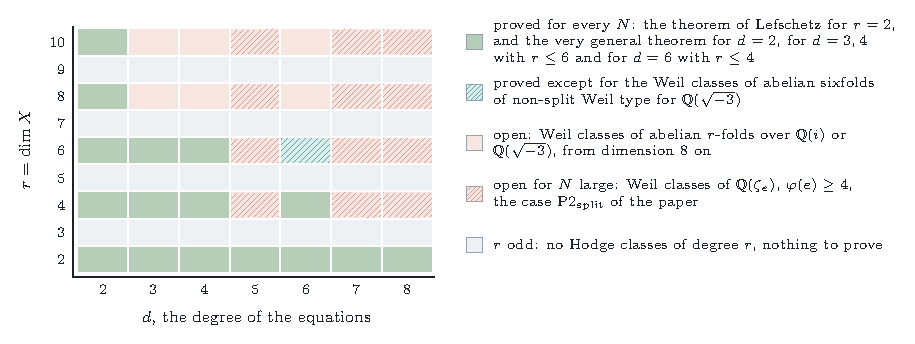
\includegraphics[width=\textwidth]{fig_vgscope}
\caption{The Hodge conjecture for the very general complete intersection
$X_{d,r}(\lambda)$ of Vandermonde type, for every $N$. Grass: proved, by the
theorem of Lefschetz for $r=2$ and by \Cref{thm:vgvandermonde} for $d=2$,
for $d=3,4$ with $r\le6$ and for $d=6$ with $r\le4$. Teal hatching: proved
except for the Weil classes of abelian sixfolds of non-split Weil type for
$\QQ(\sqrt{-3})$. Clay: open, the Weil classes of abelian varieties of Weil
type over $\QQ(i)$ or $\QQ(\sqrt{-3})$ in dimension at least eight, or,
hatched, of a CM field of degree at least four (\Cref{rem:vandermonde}).
For odd $r$ there is nothing to prove.}
\label{fig:vgscope}
\end{figure}

\begin{remark}[What the diagonal complete intersections give]
\label{rem:vandermonde}
\Cref{thm:vandermonde} adds to the domain of \textup{(F3$'$)} a family of
complete intersections of every dimension and every degree, parametrised by
configurations of $N+1$ points on the line, among them all smooth complete intersections of two diagonal
hypersurfaces; for $c\ge3$ and $r\ge2$ the condition on the columns is a real
restriction. \Cref{cor:twodiagonal} shows on them how \textup{(F3$'$)} and
(F2) together give the conjecture: once the Hodge classes of $X$ are
carried to the abelian varieties $B_{[a]}$, the conjecture for $X$ is the
algebraicity of their Hodge classes, a question of type (F2), and for the
fourfolds in $\PP^{6}$ of degrees $3$, $4$ and $6$ it is answered by
Markman's theorem: their exceptional classes are Weil classes of abelian
fourfolds of Weil type, $490$ families of them for $d=4$. For $d=3$ these
fourfolds are Fano and the conjecture also follows from the theorem of Conte
and Murre on uniruled fourfolds \cite{CM78}; for $d=4$ and $d=6$ they are of
general type, with $h^{2,2}=2584$ and $48588$. Complete intersections of
diagonal hypersurfaces, and of quadrics, are also the subject of Terasoma's
paper \cite{Ter88}. At a very general configuration
\Cref{thm:vgvandermonde} goes further, in every $\PP^{N}$: for $d=2$ in every
dimension, for $d=3$ and $d=4$ up to dimension seven, and for $d=6$ up to
dimension five, through the monodromy of cyclic covers of degree three, four
and six (\Cref{prop:cyclicmonodromy}). For $d=3$ and $r\ge8$ the
conjecture for the very general member is the algebraicity of the Weil
classes of the abelian $r$-folds $B_{[a]}$ of split Weil type for
$\QQ(\sqrt{-3})$, which is open from dimension eight on, and the same holds
for $d=4$ with $\QQ(i)$. For $d=6$ and $r=6$ the open classes are those of
the abelian sixfolds of non-split Weil type for $\QQ(\sqrt{-3})$ of
\Cref{thm:vgvandermonde}(iii), such as the one of the character
$(1,1,2,2,3,5,5,5)$ on eight points. Beyond these cases the
same reduction meets (F2) itself: for $d=5$ or $d\ge7$ and $N$ large enough, some
$B_{[a]}$ with $\dim V_{a}=r$ carries an action of $\QQ(\zeta_{e})$, $e\mid d$,
with $\varphi(e)\ge4$, and $W_{[a]}$ is the top exterior power of its first
cohomology over that CM field, which consists of Hodge classes when the
types are balanced: Weil classes for a CM field of degree at least four, of
the kind treated in \Cref{thm:main}; and for larger $N$ the $B_{[a]}$ have
dimension above five.
\end{remark}

\begin{remark}[Where \textup{(F3$'$)} stops]\label{rem:f3primefrontier}
With \Cref{prop:f3prime}, \Cref{prop:aclosure} and \Cref{prop:f3primesmall},
\textup{(F3$'$)} holds on every variety of dimension at most three, on every
fourfold whose zero-cycles are supported in dimension three (in particular
every uniruled fourfold), on every fivefold whose zero-cycles are supported
in dimension at most three, on every fourfold and fivefold whose maximal
rationally connected quotient is birational to a variety satisfying
\textup{(F3$'$)} in degree four (\Cref{prop:f3primefibration}), on every
fourfold and fivefold dominated by a rational map from such a variety
(\Cref{prop:f3primedominant}), and on
every member of $\mathcal{A}$, a class containing the Fermat
hypersurfaces, the smooth Delsarte hypersurfaces with the cyclic covers
branched along them (\Cref{cor:delsarteall}), and the complete intersections
of diagonal hypersurfaces of Vandermonde type, among them every smooth
complete intersection of two diagonal hypersurfaces (\Cref{thm:vandermonde},
\Cref{cor:twodiagonal}), of every degree and dimension, the Hilbert schemes of points on
abelian surfaces, on products of curves and on the K3 surfaces of
\Cref{prop:aclosure}(iv), the generalised Kummer varieties $K_{n}(A)$ and the
other varieties of \Cref{prop:aclosure}(v), and every blow-up and projective bundle
built from these. Through the Hodge conjecture itself it holds on the
complete intersections of \Cref{cor:twodiagonal}(ii), among them the
fourfolds of general type cut out by two diagonal quartics or sextics in
$\PP^{6}$, on the very general complete intersections of diagonal quadrics,
of diagonal cubics and quartics up to dimension seven and of diagonal
sextics up to dimension five, of \Cref{thm:vgvandermonde}, and on the
varieties of \Cref{prop:k3powers}, \Cref{prop:k3ntype} and
\Cref{cor:fanolines}: for a K3 surface $S$ with
$E=\End_{\mathrm{Hdg}}(T(S))$ a CM field, on every power, Hilbert scheme and
moduli space of $S$; for $E=\QQ$ and $t=\dim T(S)$, on $S^{k}$ for $k<t$, on
$S^{[n]}$ for $n<t(t+1)/2$ and on the moduli spaces of dimension less than
$t$; on every fourfold of K3$^{[2]}$ type whose field $E$ is $\QQ$ or a CM
field; on $F(Y)$ and $Y\times Y$ for every cubic fourfold $Y$ with such a
field; and on every fourfold of generalised Kummer type \cite{FV25}. Its
frontier cases are these (\Cref{fig:f3primereach}), the first two in
degree four on fourfolds whose zero-cycles are not supported on a proper
closed subset and which are not birational to a member of $\mathcal{A}$ by
any construction above: $S\times S$ and $S^{[2]}$ for a K3 surface
whose real multiplication is not induced by a cycle constructed so far, such
as $S_{\lambda}$
(the known cases are recalled in \Cref{rem:mumfordks}); the fourfolds of
K3$^{[2]}$ type with real multiplication, among them $F(Y)$ for a cubic
fourfold $Y$ with real multiplication, and with it $Y\times Y$; and, for a
very general K3 surface, the single class $\det T(S)$ on $S^{21}$ of
\Cref{prop:orthpowers}, equivalently the Hodge conjecture for $S^{[231]}$.
In the first two the
rational Hodge isometries \cite{Bus19,Mar24} act on $T$ by $\pm1$, and a
composite of Hodge similarities that returns to $T$ is an element $g\in E$
with $g^{2}\in\QQ$, the adjoint involution of $E$ being trivial; such
elements span only the compositum of the quadratic subfields of $E$, which is
$\QQ$ for the cubic field of $S_{\lambda}$. Apart from proving the
conjecture itself where zero-cycles are small, none of these results touches
the step that
\Cref{rem:f3primeopen} identifies: putting a Hodge class into
$\mathrm{Ab}^{p}(X)$ for a variety that no correspondence connects to an
abelian variety. \Cref{thm:closure} is unchanged, since every statement
proved here is a special case of one of the hypotheses of its rule set, not a
new rule. With the theorems of recent preprints as hypotheses, the first and
third frontier cases are settled, and the second when the N\'eron--Severi
space is isotropic or represents $-2$, for instance when the Picard number is
at least four (\Cref{cor:k3all}, \Cref{prop:k3twosmall}).
\end{remark}

\begin{figure}[tbp]
\centering
  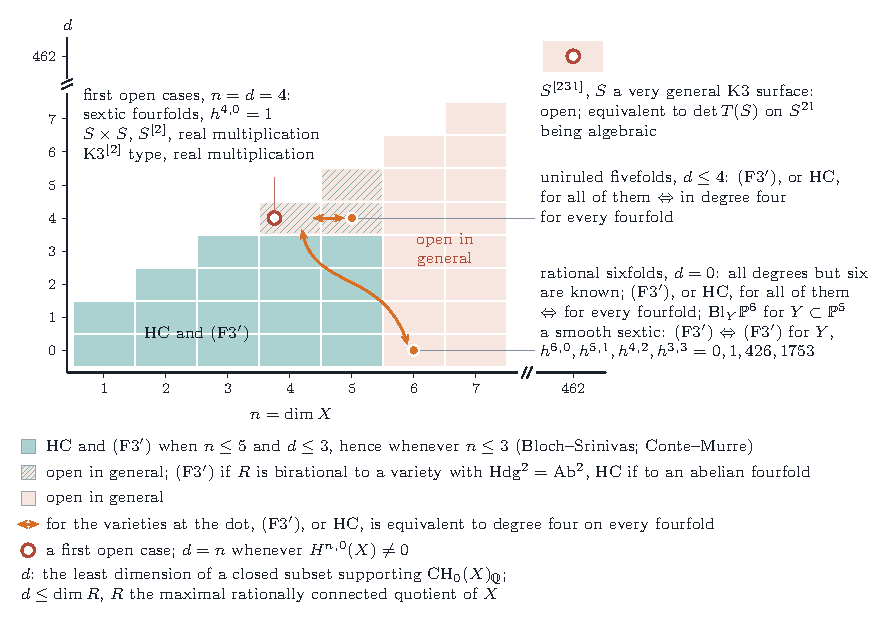
\includegraphics[width=\textwidth]{fig_f3primereach}
\caption{What arguments on zero-cycles and on rationally connected
fibrations give for \textup{(F3$'$)} and for the Hodge conjecture (HC in the
figure) on a variety $X$, over the plane of $n=\dim X$ and the least dimension
$d$ of a closed subset supporting $\mathrm{CH}_{0}(X)_{\QQ}$; $d$ is at most
the dimension of the maximal rationally connected quotient $R$ of $X$, and
$d=n$ whenever $H^{n,0}(X)\ne0$ (\Cref{rem:f3primesharp}). Both hold when
$n\le5$ and $d\le3$ (\Cref{prop:f3primesmall}), hence on every variety of
dimension at most three. In the hatched cells
\textup{(F3$'$)} holds when $R$ is birational to a variety with
$\Hdg^{2}=\mathrm{Ab}^{2}$, for instance a member of $\mathcal{A}$, and the
Hodge conjecture when $R$ is birational to an abelian fourfold
(\Cref{prop:f3primefibration}). The double arrows are the equivalences of
\Cref{rem:f3primesharp}: \textup{(F3$'$)}, and the Hodge conjecture, hold for
every uniruled fivefold, and for every rational sixfold, if and only if they
hold in degree four for every fourfold; the sixfold $\mathrm{Bl}_{Y}\PP^{6}$
of a smooth sextic fourfold $Y$ in a hyperplane carries the Hodge numbers
listed. The rings are the frontier cases (\Cref{rem:f3primefrontier}): the
sextic fourfolds, the first family of smooth hypersurfaces beyond these
results
(the $29$ Delsarte sextics lie in $\mathcal{A}$ by
\Cref{cor:delsarteall}); $S\times S$ and $S^{[2]}$ for a K3
surface $S$ with real multiplication, such as
$S_{\lambda}$; the fourfolds of K3$^{[2]}$ type with real multiplication,
among them $F(Y)$; and, beyond the breaks of the axes, $S^{[231]}$ for a very
general K3 surface, which is equivalent to the algebraicity of $\det T(S)$ on
$S^{21}$ (\Cref{prop:k3powers}, \Cref{fig:k3threshold}).}
\label{fig:f3primereach}
\end{figure}

\begin{setupenv}[The rule set]\label{setup:rules}
The rule set has forty-two statements and twenty-two rules. Ten statements
are proved in this paper: the base point with an explicit cycle in every Weil
family of an imaginary quadratic field (\Cref{thm:everyfamily}) and of a CM
field of degree at least four (\Cref{thm:cmbasepoint}); for each of the two
kinds of field, the reduction of the Weil classes of a family to one class at
every point of one connected domain, and the stability of the algebraic locus
under the rational points, with dense orbits (\Cref{sec:reduction},
\Cref{prop:densealg}, \Cref{thm:cmpropagation}); and four statements on
secant objects: the form of the weakened criterion for the transform
(\Cref{thm:factor}), the conditions of Markman's strategy that bear on the
Chern character, the description of the local obstruction as a failure of
Cohen--Macaulayness (\Cref{cor:cmdichotomy}), and three of the four
ingredients of the construction in every dimension. Four are quoted:
$\mathbf{W}(K,2,\delta)$ for every $K$ and $\delta$, $\mathbf{W}(K,3,\delta_{0})$
\cite{Mar25a,Mar25b}, the deformation theorem for motivated classes
\cite[Th\'eor\`eme~0.5]{And96b}, and the accessibility of Hodge classes on
abelian varieties \cite[\S5.1, Theorem~3]{Mil20}. Sixteen are hypotheses:
(F3), (F2) of \Cref{cor:fourremain} and (F3$'$) of \Cref{def:f3prime};
(L), (M), (V) of \Cref{def:lmv}; (P2), in the polarised form of
\Cref{rem:p2prime}, for four groups of families, the split and the other
families of the imaginary quadratic fields and of the CM fields of degree at
least four, the third group giving $\mathrm{P2}_{\mathrm{split}}$; secant
objects meeting the weakened criterion in every dimension, and an affirmative
answer to \cite[Question~11.4]{Mar25b}; and, for a smooth and for a singular
Cohen--Macaulay support on an abelian fourfold, its existence with the
required extension property and the vanishing of the image of the product of
translation classes. The other twelve are derived: $\mathbf{HC}$, the
conjecture for every abelian variety, written $\mathbf{AB}$, and the Weil
classes of every CM field, of the imaginary quadratic fields, of their
families of trivial and of nontrivial discriminant, of the CM fields of
degree at least four and of their split and their other families, together
with one secant object on an abelian fourfold, $\mathbf{W}(K,4,\delta_{0})$,
and the range settled in the literature. Each rule is a finite set of
premises with one conclusion, and each is a theorem of this paper:
\Cref{tab:rules} lists twenty-one of them, and the twenty-second derives the
range settled in the literature from the two quoted Weil statements. For a
set $T$ of statements write $\Cn(T)$ for the least set that contains $T$ and
is closed under the rules, which exists because each rule has a single
conclusion and the consequence operator is therefore monotone. Write
$\mathbf{T}$ for the set of statements proved or quoted. Call a set $S$ of
hypotheses \emph{sufficient} if $\mathbf{HC}\in\Cn(\mathbf{T}\cup S)$, and
\emph{minimal} if no proper subset of $S$ is sufficient.
\end{setupenv}

\begin{table}[htbp]
\centering
\small
\renewcommand{\arraystretch}{1.14}
\begin{tabular}{@{}>{\raggedright\arraybackslash}p{0.40\linewidth}>{\raggedright\arraybackslash}p{0.27\linewidth}l@{}}
\toprule
premises & conclusion & by \\
\midrule
the conjecture for abelian varieties, (F3)
  & $\mathbf{HC}$ & \Cref{ssec:closuremap} \\
(F3)
  & abelian varieties & \Cref{prop:f3ishc} \\
the conjecture for abelian varieties, (F3$'$)
  & $\mathbf{HC}$ & \Cref{prop:f3prime} \\
the Weil classes of every CM field, (F2)
  & abelian varieties & \Cref{ssec:closuremap} \\
$K$ imaginary quadratic, the fields of degree at least four
  & every CM field & \Cref{app:albert} \\
$\delta=\delta_{0}$, $\delta\ne\delta_{0}$
  & every discriminant & \Cref{prop:separate} \\
a base point, the reduction, the orbit, (P2) for the family
  & that family & \Cref{thm:semiregclosure} \\
the same three for a CM field of degree at least four, (P2) for the family
  & that family & \Cref{thm:cmpropagation} \\
its split families, its other families
  & the fields of degree at least four & \Cref{prop:cmweil} \\
$\delta=\delta_{0}$
  & $\delta\ne\delta_{0}$ & \Cref{prop:descent} \\
the split families of the fields of degree at least four
  & their other families; $\delta=\delta_{0}$ & \Cref{prop:descent} \\
a secant object in every dimension, Question 11.4
  & $\delta=\delta_{0}$ & \Cref{prop:splitgeom} \\
a Cohen--Macaulay support, smooth or singular
  & one secant object & \Cref{cor:cmdichotomy} \\
one secant object, Question 11.4
  & $\mathbf{W}(K,4,\delta_{0})$ & \Cref{cor:markmancondition} \\
\midrule
(L), (M)
  & $\mathbf{HC}$ & \Cref{prop:lefmot} \\
(L), the deformation theorem for motivated classes
  & (V) & \Cref{prop:lefvhc} \\
(V), the accessibility of Hodge classes on abelian varieties
  & abelian varieties & \Cref{thm:vhcab} \\
\bottomrule
\end{tabular}
\caption{The rules of \Cref{setup:rules} whose conclusion is derived, with the
theorem that proves each; the rows for (P2) and for the Cohen--Macaulay
support each stand for two rules, the row for descent over the fields of
degree at least four for two, descent within a field and scalar extension
down to the imaginary quadratic fields, the second row is \Cref{prop:f3ishc},
the third is
\Cref{prop:f3prime}(i) for the weaker statement (F3$'$) of
\Cref{def:f3prime}, the last three rows are the rules of
\Cref{ssec:bullseye}, one of whose conclusions, (V), is itself a
hypothesis of the rule set, and the one remaining rule records what the literature supplies on Weil classes. The
bounded criterion (P1) is absent: by
\Cref{thm:p1equivalent} it is equivalent to its own conclusion, so it is a
restatement and not a premise.}
\label{tab:rules}
\end{table}

\begin{theorem}[The closure of what is proved here]\label{thm:closure}
With the notation of \Cref{setup:rules}:
\begin{enumerate}[label=\textup{(\roman*)},leftmargin=2.6em]
\item $\mathbf{HC}\notin\Cn(\mathbf{T})$. Nothing in this paper, combined with the
  theorems it quotes, implies the Hodge conjecture.
\item There are exactly five minimal sufficient sets:
  \[
    \{\mathrm{F3}\},\quad\{\mathrm{L},\mathrm{M}\},\quad
    \{\mathrm{L},\mathrm{F3}'\},\quad\{\mathrm{V},\mathrm{F3}'\},\quad
    \{\mathrm{P2}_{\mathrm{split}},\mathrm{F2},\mathrm{F3}'\},
  \]
  with \textup{(L)}, \textup{(M)}, \textup{(V)} as in \Cref{def:lmv},
  \textup{(F2)}, \textup{(F3)} as in \Cref{cor:fourremain}, (F3$'$) as in
  \Cref{def:f3prime}, and $\mathrm{P2}_{\mathrm{split}}$ the propagation
  statement \textup{(P2)}, read in the polarised form of \Cref{rem:p2prime},
  for the split families of the CM fields of degree at least four. No
  minimal set contains \textup{(P2)} for an imaginary quadratic field or for
  a family of nontrivial discriminant: \Cref{prop:descent} derives those.
  The single hypothesis (F3) is sufficient, and it is equivalent to
  $\mathbf{HC}$ (\Cref{prop:f3ishc}); no other single hypothesis is.
  The sets $\{\mathrm{L},\mathrm{F3}\}$, $\{\mathrm{V},\mathrm{F3}\}$ and
  $\{\mathrm{P2}_{\mathrm{split}},\mathrm{F2},\mathrm{F3}\}$ are sufficient and
  not minimal. The last of the five is the only one with three elements and the
  only one whose derivation of $\mathbf{HC}$ uses a statement proved in this
  paper.
\item In each of the five, every element is necessary: removing any one
  leaves $\mathbf{HC}$ outside the closure.
\item The secant route lies in no minimal sufficient set. Granting both of its
  demands, a secant object satisfying the weakened criterion in every
  dimension and an affirmative answer to \cite[Question 11.4]{Mar25b}, puts
  $\mathbf{W}(K,n,\delta_{0})$ in the closure, and with it, by
  \Cref{prop:descent}, $\mathbf{W}(K,n,\delta)$ for every $\delta$; it leaves
  the Weil classes of the CM fields of degree at least four outside.
\item No statement proved in this paper rests, at any depth, on a
  hypothesis, and the rule set is acyclic.
\item Every element of a minimal sufficient set other than
  $\mathrm{P2}_{\mathrm{split}}$ is a consequence of $\mathbf{HC}$, and $\{\mathrm{F3}\}$ and
  $\{\mathrm{L},\mathrm{M}\}$ are each equivalent to it; no implication from
  $\mathbf{HC}$ to \textup{(P2)} is known.
\end{enumerate}
\end{theorem}

\begin{proof}
(i) and (v). No rule has a proved or quoted statement as its conclusion, so
each of them lies in $\Cn(\mathbf{T})$ by itself, on the strength of its proof
in this paper or in the literature; this is the first assertion of (v). The
twenty-second rule is the only one whose premises all lie in $\mathbf{T}$:
every other rule has among its premises a hypothesis or a derived statement
other than the range settled in the literature. Hence $\Cn(\mathbf{T})$ is
$\mathbf{T}$ together with that range, and it does not contain $\mathbf{HC}$,
which is (i). For acyclicity, list first the thirty statements that are
proved, quoted or hypotheses other than (V); then one secant object,
$\mathbf{W}(K,4,\delta_{0})$ and the range settled in the literature; the
split and then the other families of the CM fields of degree at least four;
the families of trivial and then of nontrivial discriminant of the imaginary
quadratic fields; the imaginary quadratic fields, the CM fields of degree at
least four and every CM field; and last (V), $\mathbf{AB}$ and $\mathbf{HC}$.
The premises of every rule come before its conclusion in this list.

(ii) and (iii). The five sets are sufficient:
$\mathrm{F3}\Rightarrow\mathbf{AB}$ (\Cref{prop:f3ishc}) and
$\mathbf{AB}\wedge\mathrm{F3}\Rightarrow\mathbf{HC}$; $\mathrm{L}\wedge
\mathrm{M}\Rightarrow\mathbf{HC}$ (\Cref{prop:lefmot}); (L) and the
deformation theorem give (V) (\Cref{prop:lefvhc}), (V) and accessibility give
$\mathbf{AB}$ (\Cref{thm:vhcab}), and $\mathbf{AB}\wedge\mathrm{F3}'
\Rightarrow\mathbf{HC}$ (\Cref{prop:f3prime}(i)), which settles
$\{\mathrm{L},\mathrm{F3}'\}$ and $\{\mathrm{V},\mathrm{F3}'\}$; and
$\mathrm{P2}_{\mathrm{split}}$ with the CM base point, the reduction and the
orbit gives the split families of the CM fields of degree at least four
(\Cref{thm:cmpropagation}), descent gives their other families and the
families of trivial discriminant of the imaginary quadratic fields
(\Cref{prop:descent}), hence the fields of degree at least four
(\Cref{prop:cmweil}), the nontrivial discriminant (\Cref{prop:descent}),
the imaginary quadratic fields (\Cref{prop:separate}) and every CM field
(\Cref{app:albert}), and with (F2) this is $\mathbf{AB}$ and with (F3$'$)
it is $\mathbf{HC}$.

Let $C_{1}$, respectively $C_{2}$, be the set of all statements other than
$\mathbf{HC}$, (F3), (F3$'$) and (L), respectively (M). Let $C_{3}$ be the
set of all statements other than $\mathbf{HC}$, $\mathbf{AB}$, the Weil
classes of every CM field, of the fields of degree at least four and of their
split families, (F3), (L), (V) and $\mathrm{P2}_{\mathrm{split}}$; and let
$C_{4}$ be the set of all statements other than $\mathbf{HC}$,
$\mathbf{AB}$, (F3), (L), (V) and (F2). Each $C_{j}$ contains $\mathbf{T}$
and not $\mathbf{HC}$, and each is closed under the rules: every rule whose
conclusion it omits has a premise it omits. For $C_{1}$ and $C_{2}$ the only
omitted conclusion is $\mathbf{HC}$, and the three rules with that
conclusion have the premises (F3), (F3$'$), and (L) and (M). For $C_{3}$
and $C_{4}$ the rules with conclusion $\mathbf{HC}$ have the premises
$\mathbf{AB}$ or (L); those with conclusion $\mathbf{AB}$ have the premises
(F3), the Weil classes of every CM field together with (F2), and (V); the
only rule with conclusion (V) has the premise (L); and for $C_{3}$ the rule
for every CM field needs the fields of degree at least four, the rule for
these needs their split families, and the rule for the split families needs
$\mathrm{P2}_{\mathrm{split}}$. Since $\Cn$ is monotone, a set of
hypotheses contained in some $C_{j}$ has its closure, together with
$\mathbf{T}$, inside $C_{j}$, and is not sufficient. So a sufficient set
meets each of
\begin{gather*}
  H_{1}=\{\mathrm{F3},\mathrm{F3}',\mathrm{L}\},\qquad
  H_{2}=\{\mathrm{F3},\mathrm{F3}',\mathrm{M}\},\\
  H_{3}=\{\mathrm{F3},\mathrm{L},\mathrm{V},\mathrm{P2}_{\mathrm{split}}\},\qquad
  H_{4}=\{\mathrm{F3},\mathrm{L},\mathrm{V},\mathrm{F2}\},
\end{gather*}
the hypotheses omitted from $C_{1},\dots,C_{4}$. Let $S$ meet all four. If
$\mathrm{F3}\in S$, then $S\supseteq\{\mathrm{F3}\}$. If $\mathrm{F3}\notin S$
and $\mathrm{L}\in S$, then $S$ meets $H_{2}$ in (F3$'$) or (M). If neither is
in $S$, then $S$ contains (F3$'$), from $H_{1}$, and (V) or both
$\mathrm{P2}_{\mathrm{split}}$ and (F2), from $H_{3}$ and $H_{4}$. So a set
of hypotheses is sufficient exactly when it contains one of the five sets,
and as none of the five contains another, they are the minimal sufficient
sets. The other assertions of (ii) can be read off the list, and the
derivations above show that only the last uses a statement proved here;
(iii) is the minimality.

(iv) Granting the two demands of the secant route, the rule of
\Cref{prop:splitgeom} gives the families of trivial discriminant, descent
those of nontrivial discriminant, and \Cref{prop:separate} the imaginary
quadratic fields. The set formed by $\mathbf{T}$, the range settled in the
literature, the two demands and these three statements is closed, since
every other rule has a premise outside it: a hypothesis not granted, one
secant object, or a Weil statement about the fields of degree at least four
or about every CM field. Every base point the secant route produces is a
member $X\times\widehat{X}$, whose discriminant is trivial whatever $\beta$
is chosen (\Cref{prop:splitgeom}(ii)); the deformation argument stays inside
the family of trivial discriminant, and it is \Cref{prop:descent}(i), not
the deformation, that carries the result to the other discriminants. The
route has no base point over a field of degree at least four, so it reaches
none of them, and none of its hypotheses lies in one of the five sets.

(vi) \textup{(L)} follows from $\mathbf{HC}$ by \Cref{thm:equivalence},
\textup{(M)} by \Cref{prop:lefmot}, \textup{(V)} by \Cref{prop:lefvhc},
(F3$'$) by \Cref{prop:f3prime}(i), and (F2) and (F3) are special cases of
$\mathbf{HC}$. The equivalence of $\{\mathrm{F3}\}$ with $\mathbf{HC}$ is
\Cref{prop:f3ishc}, and $\{\mathrm{L},\mathrm{M}\}$ is equivalent to it by
\Cref{prop:lefmot} and the first two implications.
\end{proof}

\begin{corollary}[The three statements, one of which is the
conjecture]\label{cor:fourremain}
The Hodge conjecture follows from the results of this paper together with the
following three statements. No rule of \Cref{setup:rules} derives it from
(F1) and (F2) together, and it follows from (F3) alone, which is equivalent
to it
(\Cref{prop:f3ishc}); so the list is not a reduction of the conjecture to
three smaller problems. With (F3) replaced by the weaker statement
\textup{(F3$'$)} of \Cref{def:f3prime}, the conjecture modulo abelian
varieties, the three statements (F1), (F2), \textup{(F3$'$)} still suffice,
and no rule of \Cref{setup:rules} derives the conjecture from a proper
subset of them. With the rule of \Cref{prop:f2isab}, which the rule set does
not contain, (F2) and \textup{(F3$'$)} already suffice (\Cref{rem:f2rule}).
\begin{enumerate}[label=\textup{(F\arabic*)},leftmargin=3.0em,itemsep=4pt]
\item \emph{One propagation statement, for every CM field.} \textup{(P2)},
  in the polarised form of \Cref{rem:p2prime}: at one base point of each
  Weil family of each CM field some perfect complex whose Chern character is
  a nonzero multiple of a rational Weil class plus a polynomial in the
  polarisation has injective semiregularity map. Its first form, with Chern
  character exactly a multiple of the Weil class, is false for every
  imaginary quadratic field and every $n\ge2$ (\Cref{thm:p2false}): such a
  complex would have to deform to non-algebraic Weil tori, whose coherent
  sheaves have no Chern character in degrees $1$ to $2n-1$. The polarised form
  closes
  $\mathbf{W}(K,n,\delta)$
  for every imaginary quadratic $K$, every $n$ and every $\delta$ at once, by
  \Cref{thm:semiregclosure}, and
  $\mathbf{W}(F,n,\delta)$ for every CM field $F$ of higher degree, by
  \Cref{thm:cmpropagation}, because those theorems put $\Sigma=\cD$, so the
  Weil class is algebraic at every member of the family and not only at the
  general one, and because \Cref{thm:everyfamily} and \Cref{thm:cmbasepoint}
  supply the base point in every one of those families. By
  \Cref{prop:descent} it is enough to have it for the split families of the
  CM fields of degree at least four, in infinitely many dimensions.
  \Cref{thm:p2forces}, \Cref{thm:p2support}, \Cref{thm:nosum},
  \Cref{thm:p2numerical} and \Cref{thm:p2endo} describe the object of the
  first form and are vacuous by \Cref{thm:p2false}; for the polarised form
  \Cref{thm:p2primenumber} computes the number that $\dim\Ext^{2}(E,E)$ has
  to reach, $7n^{2}-2n$ for a general shape. For one family its
  conclusion is equivalent to the Lefschetz standard conjecture for one
  variety (\Cref{cor:weilequiv}). The bounded criterion \textup{(P1)} is not a
  second form of the same demand: by
  \Cref{thm:p1equivalent} it is equivalent to the conclusion it was to imply,
  and \Cref{thm:p1forces} shows that the one cycle it could have been tested
  on, the transport of the base cycle, does not satisfy it.
\item \emph{The classes beyond the Weil lines.} Every Hodge class on an
  abelian variety that lies outside the subring generated by divisor classes
  and by Weil classes of quotients is algebraic. Through dimension five there
  is no such class \cite{MZ99}; in dimension eight there are
  (\Cref{prop:mumfordproduct}), so this is not a reduction of the conjecture
  for abelian varieties to Weil classes, which is false as a statement about
  Hodge rings: it is the conjecture for those classes, and by
  \Cref{prop:f2isab} it is equivalent to the conjecture for every abelian
  variety. Its smallest case is
  brought down to one Kuga--Satake class in \Cref{thm:mumfordks}; it holds at
  every CM point (\Cref{thm:mumfordcm}), and on all members of a Mumford
  family it is equivalent to the Lefschetz standard conjecture for one
  ninefold (\Cref{cor:mumfordequiv}). Its classes are rigid along the base
  curve (\Cref{thm:mumfordrigid}), and one complex at one CM point with
  $\Ext^{2}$ of dimension $119$ would close it (\Cref{thm:mumfordnumerical}),
  as would a bound on the cycles that represent them at the closed points of
  the reductions of the curve modulo primes (\Cref{thm:modpdensity}).
\item \emph{The varieties that are not abelian.} The Hodge conjecture holds
  for every smooth complex projective variety that is not an abelian variety.
  This is the Hodge conjecture itself. The varieties it covers include
  $A\times\PP^{1}$ for every abelian variety $A$, and the conjecture for
  $A\times\PP^{1}$ gives it for $A$ (\Cref{prop:f3ishc}); so (F3) implies
  the conjecture for abelian varieties, hence (F1) and (F2), and hence
  $\mathbf{HC}$. Nor is it a reduction to abelian varieties in the other
  direction: no realisation of the cohomology of an arbitrary variety inside
  that of abelian varieties exists (\Cref{prop:noabeliantype}), and
  \Cref{thm:hyperplane} and \Cref{thm:returntrip} close the two routes
  through hyperplane sections that would be the natural candidates for one.
\end{enumerate}
\end{corollary}

\begin{proof}
The three together are sufficient by the derivation of \Cref{thm:closure},
and (F3) alone by \Cref{prop:f3ishc}. That (F1) and (F2) together are not
sufficient in the rule set is \Cref{thm:closure}(ii), since every minimal
sufficient set contains (F3), \textup{(F3$'$)} or \textup{(M)}; the
statement about (F1), (F2), \textup{(F3$'$)} is \Cref{thm:closure}(ii) and
(iii) for the last of the five minimal sets. The Weil classes of the CM
fields of degree at least four are not a fourth statement: they are derived
from (F1) by \Cref{thm:cmpropagation}. Nor is the bounded criterion a
premise, since by \Cref{thm:p1equivalent} it is a restatement of its own
conclusion.
\end{proof}

\begin{remark}[Necessity relative to a rule set, and the wording of (F2)]
\label{rem:f3collapse}
A rule set can show that a set of statements suffices; it can show that a set
is needed only relative to the implications written into it. A rule set that
used (F3) only through $\text{(abelian varieties)}\wedge
\text{(F3)}\Rightarrow\mathbf{HC}$, without the elementary rule
$\text{(F3)}\Rightarrow\text{(abelian varieties)}$ of \Cref{prop:f3ishc},
would make the three statements of \Cref{cor:fourremain} look jointly
necessary, although (F3) alone suffices.

The wording of (F2) has the same feature, one degree at a time. Let
$R(A)\subseteq H^{*}(A,\QQ)$ be the subring generated by divisor classes and
Weil classes of quotients. Suppose some Hodge class $\beta$ of degree $2p$ on
$A$ lies outside $R(A)$, and let $\alpha$ be any Hodge class of degree $2p$.
If $\alpha\notin R(A)$, (F2) makes it algebraic. If $\alpha\in R(A)$, then
$\alpha+\beta\notin R(A)$, because $R(A)$ is closed under subtraction, so
(F2) makes $\alpha+\beta$ and $\beta$ algebraic, and with them $\alpha$.
So in every degree in which (F2) says anything it is the whole conjecture for
that degree: on the square of a Mumford fourfold it gives every Hodge class of
$H^{4}$, the six products of divisor classes included. Multiplying by an
exceptional class of that square moves every Hodge class of every abelian
variety outside the subring, and \Cref{prop:f2isab} deduces from this that
(F2) is the whole conjecture for abelian varieties. The rule set does not
contain that implication; \Cref{rem:f2rule} says how \Cref{thm:closure}(ii)
changes when it is adjoined.

The form of (F3) that is not the conjecture itself asks only for
algebraicity modulo classes coming from abelian varieties. It is
\textup{(F3$'$)} of \Cref{def:f3prime}; \Cref{prop:f3prime} says what is
known of it, and \Cref{rem:f3primeopen} why it is not closed.
\end{remark}

\begin{figure}[tbp]
\centering
  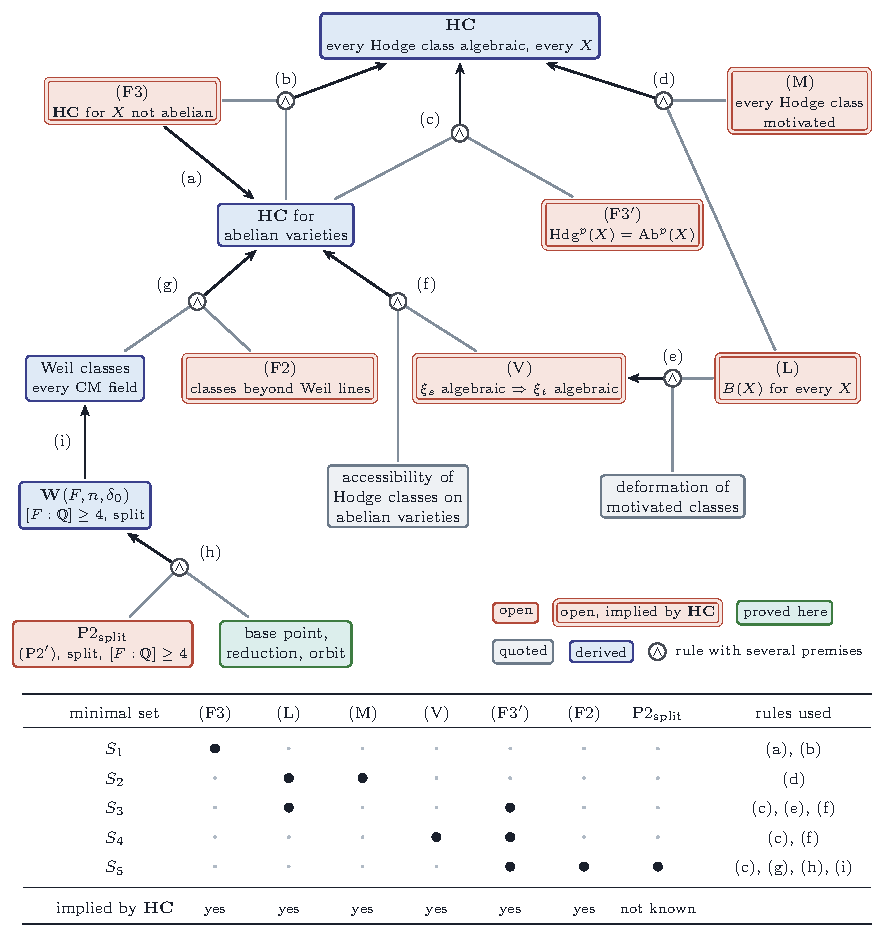
\includegraphics[width=0.92\textwidth]{fig_frontier}
\caption{The rule set of \Cref{setup:rules} with the rules of
\Cref{ssec:bullseye}, drawn as a hypergraph. A rule with several premises is
a junction marked $\wedge$, joined to its premises and with one arrow to its
conclusion. The letters name the results that prove the rules: (a) is
\Cref{prop:f3ishc}; (b) and (g) are the closure map of
\Cref{ssec:closuremap}; (c) is \Cref{prop:f3prime}(i); (d) is
\Cref{prop:lefmot}; (e) is \Cref{prop:lefvhc}; (f) is \Cref{thm:vhcab};
(h) is \Cref{thm:cmpropagation}; and (i) is the chain of
\Cref{prop:descent}, \Cref{prop:separate}, \Cref{prop:cmweil} and
\Cref{app:albert}. Clay marks a hypothesis, a double frame a hypothesis
that the conjecture implies, grass what this paper proves, slate
what it quotes, and indigo a derived statement. The table lists the five
minimal sufficient sets of \Cref{thm:closure}(ii), the rules each of them
uses, and which of the hypotheses the conjecture implies; only
$\mathrm{P2}_{\mathrm{split}}$, which asks for a particular complex, is
drawn without that frame. The secant route, which reaches the imaginary
quadratic families only, is drawn in \Cref{fig:closure}.}
\label{fig:frontier}
\end{figure}

\begin{remark}[The target, and what it would take]\label{rem:bullseye}
With the rules of \Cref{ssec:bullseye}, \Cref{prop:f3ishc} and
\Cref{prop:f3prime} in place, \Cref{thm:closure} changes the reading of
\Cref{cor:fourremain} in three ways. First, the route through this paper is
a route only with (F3) replaced by \textup{(F3$'$)}. As stated, its last
statement (F3) is the conjecture (\Cref{prop:f3ishc}), so (F1) and (F2), and
everything this paper proves about Weil classes, drop out of every minimal
derivation that uses (F3). With \textup{(F3$'$)} in its place the route
$\{\mathrm{P2}_{\mathrm{split}},\mathrm{F2},\mathrm{F3}'\}$ is minimal, and it is not the
shortest: (F1) and (F2), which between them give the conjecture for abelian
varieties along this route, are replaced on the routes of the literature by
the single statement \textup{(V)} (\Cref{thm:vhcab}), or by \textup{(L)},
which implies it (\Cref{prop:lefvhc}). Second, every element of every minimal sufficient set
except $\mathrm{P2}_{\mathrm{split}}$ is a consequence of the conjecture
(\Cref{thm:closure}(vi)), and
two of the sets, $\{\mathrm{F3}\}$ and $\{\mathrm{L},\mathrm{M}\}$, are
each equivalent to it. (P2) is a statement about semiregularity maps, and a
proof of the conjecture need not prove it; in its first form, with a Chern
character that is exactly a Weil class, it is false (\Cref{thm:p2false}), and
the route runs through the polarised form of \Cref{rem:p2prime}. Third, every minimal sufficient set
contains (F3), \textup{(F3$'$)} or \textup{(M)}: the varieties that are not
abelian are reached only through the conjecture for them, which is the whole
conjecture, through the conjecture modulo abelian varieties
(\Cref{rem:f3primeopen}), or through motivated classes.

So the target at the centre is \textup{(L)}. It lies in two of the five
minimal sets, it gives \textup{(V)} and with it the whole abelian half, the
conjecture implies it, and with \textup{(M)} it is the conjecture. For each
$X$ it asks for one explicit Hodge class on $X\times X$ to be algebraic, the
class inducing $\Lambda$. This paper proves \textup{(L)}, \textup{(M)},
\textup{(V)} and \textup{(F3$'$)} on the classes of varieties named here:
\Cref{cor:mumfordlefschetz} adds the total spaces of Mumford families to the
known cases of \textup{(L)}, \Cref{prop:f3prime} records the known cases of
\textup{(F3$'$)}, and the routes of the literature use no other theorem of
this paper.
\end{remark}

\subsubsection*{Two of the three are not reductions}

One could hope that (F2) and (F3) are reductions in the ordinary sense,
statements to the effect that every Hodge class is carried, by some
correspondence, to a class on a Weil type variety or on an abelian variety,
so that the whole conjecture would follow from the Weil classes alone. Both
hopes are refutable, and we refute them, because a frontier that contains a
false statement is not a frontier.

\begin{proposition}[The Hodge ring is not generated by divisor and Weil
classes]\label{prop:mumfordproduct}
Let $X$ be a complex abelian fourfold whose Hodge group is a $\QQ$-form of an
almost direct product of three copies of $\mathrm{SL}_{2}$, acting on
$V=H^{1}(X,\QQ)$ through the tensor product $V_{1}\otimes V_{2}\otimes V_{3}$
of the three standard representations, with $\End^{0}(X)=\QQ$; such
fourfolds exist and form families of dimension one, by Mumford
\cite{Mum69}, and by \cite[2.5(i)]{MZ99} they are exactly the fourfolds
with $\End^{0}(X)=\QQ$ and Hodge group smaller than $\Sp_{8}$. Then:
\begin{enumerate}[label=\textup{(\roman*)},nosep,leftmargin=2.6em]
\item the Hodge ring of $X$ is generated by the polarisation:
  $\dim_{\QQ}\Hdg^{1}(X)=\dim_{\QQ}\Hdg^{2}(X)=1$;
\item $\dim_{\QQ}\Hdg^{1}(X\times X)=3$ and $\dim_{\QQ}\Hdg^{2}(X\times X)=8$,
  while the products of divisor classes span a subspace of dimension $6$
  in $H^{4}(X\times X,\QQ)$;
\item the two remaining classes lie in $H^{4}(X\times X,\QQ)$ and are Weil
  classes of no CM field acting on $X\times X$, on a quotient of it, or on an
  abelian subvariety of it.
\end{enumerate}
In particular the statement that every Hodge class on an abelian variety
lies in the subring generated by divisor classes and Weil classes of
quotients is false in dimension eight, though true through dimension five
\cite{MZ99}.
\end{proposition}

\begin{proof}
Hodge classes are the invariants of the Hodge group, so
$\Hdg^{k}(Y)\otimes\CC$ is the space of $\Hg(Y)_{\CC}$-invariants in
$\bigwedge^{2k}H^{1}(Y,\CC)$, and $\Hg(X\times X)=\Hg(X)$ acting
diagonally on $V\oplus V$. Over $\CC$ the group is
$\mathrm{SL}_{2}^{3}$ and the weights of $V$ under its maximal torus are the
eight sign vectors $(\pm1,\pm1,\pm1)$. Write $V=V_{1}\otimes W$ with
$W=V_{2}\otimes V_{3}$, on which $\mathrm{SL}_{2}^{2}=\mathrm{Spin}(4)$ acts
orthogonally. The Cauchy formula
$\bigwedge^{k}(V_{1}\otimes W)=\bigoplus_{|\lambda|=k}S_{\lambda}V_{1}\otimes
S_{\lambda'}W$ \cite[\S6.1]{FH91}, with $S^{2}V_{1}=S_{(3,1)}V_{1}=V(2)$,
$\bigwedge^{2}V_{1}=S_{(2,2)}V_{1}=\mathbf{1}$ and $S^{4}V_{1}=V(4)$, gives
$\bigwedge^{2}V=V(2)\otimes\bigwedge^{2}W\oplus S^{2}W$ and
$\bigwedge^{4}V=V(4)\otimes\bigwedge^{4}W\oplus V(2)\otimes S_{(2,1,1)}W
\oplus S_{(2,2)}W$. Under $\mathrm{Spin}(4)$, $\bigwedge^{2}W=V(2,0)\oplus
V(0,2)$, $S^{2}W=V(2,2)\oplus\mathbf{1}$, $\bigwedge^{4}W=\mathbf{1}$,
$S_{(2,1,1)}W\cong\mathfrak{sl}(W)=\bigwedge^{2}W\oplus S^{2}_{0}W$, and
$S_{(2,2)}W=V(4,0)\oplus V(0,4)\oplus V(2,2)\oplus\mathbf{1}$, the
decomposition of the algebraic curvature tensors in dimension four into the
self-dual and anti-self-dual Weyl parts, the traceless Ricci part and the
scalar part. Hence
\begin{gather*}
  \textstyle\bigwedge^{2}V=V(2,2,0)\oplus V(2,0,2)\oplus V(0,2,2)\oplus\mathbf{1},\\
  \textstyle\bigwedge^{4}V=V(2,2,2)\oplus\bigoplus_{\text{cyc}}V(4,0,0)
  \oplus\bigoplus_{\text{cyc}}V(2,2,0)\oplus\mathbf{1},
\end{gather*}
each with one trivial summand, which is (i). For (ii),
$\bigwedge^{4}(V\oplus V)=\bigoplus_{a}\bigwedge^{a}V\otimes\bigwedge^{4-a}V$
and the invariants in $\bigwedge^{a}V\otimes\bigwedge^{4-a}V$ are
$\Hom_{\mathrm{SL}_{2}^{3}}(\bigwedge^{a}V,\bigwedge^{4-a}V)$, since every
summand is self-dual; the counts are $1,1,4,1,1$, total $8$, the $4$ coming
from the four distinct irreducible summands of $\bigwedge^{2}V$. Likewise the
invariants in $\bigwedge^{2}(V\oplus V)$ number $1+1+1=3$. The divisor
classes of $X\times X$ are the three symplectic forms $\psi_{11}$, $\psi_{12}$,
$\psi_{22}$ on $V\oplus V$ built from the polarisation $\psi$ of $V$. Their
six pairwise products are linearly independent: they lie in the summands
$\bigwedge^{a}V\otimes\bigwedge^{4-a}V$ with $a=4,3,2,2,1,0$, each is
nonzero, and in the summand $a=2$ the classes $\psi_{11}\psi_{22}$ and
$\psi_{12}^{2}$ correspond, as maps $\bigwedge^{2}V\to\bigwedge^{2}V$, to a
multiple of the projection onto $\CC\psi$ and to a multiple of the
identity. The $\Sp_{8}$-invariants of $\bigwedge^{4}(V\oplus V)$ number
$1+1+2+1+1=6$ by the same count, since $\bigwedge^{1}V=V$,
$\bigwedge^{2}V=\bigwedge^{2}_{0}V\oplus\mathbf{1}$ and
$\bigwedge^{3}V=\bigwedge^{3}_{0}V\oplus V$ under $\Sp_{8}$; so the six
products are all the classes a Hodge group equal to $\Sp_{8}$ would allow. For (iii), the Weil classes of an abelian
variety $Y$ with respect to a CM field $F\subseteq\End^{0}(Y)$ are, by
definition, the classes in $\bigwedge^{2k}_{F}H^{1}(Y,\QQ)\subseteq
H^{2k}(Y,\QQ)$ with $2k=\dim_{F}H^{1}(Y,\QQ)$ (\Cref{setup:cmfield}). A CM
field acting on $X\times X$ lies in $\End^{0}(X\times X)=M_{2}(\QQ)$, so it is
imaginary quadratic, $2k=8$, and its Weil classes lie in $H^{8}$, while the two
classes of (ii) have degree four. Every proper
abelian subvariety and every proper quotient of $X\times X$ is isogenous to
$X$, because $X$ is simple, and $\End^{0}(X)=\QQ$ contains no CM field, so $X$
carries no Weil classes at all. This is the statement of \cite[0.1(iii)]{MZ99}
that the exceptional classes of $X\times X$ are not of Weil type. The last
sentence is (ii) and (iii) together with the theorem of \cite{MZ99} for
dimension at most five.
\end{proof}

\begin{proposition}[No Hodge-theoretic reduction to abelian varieties]
\label{prop:noabeliantype}
Let $Y$ be a very general smooth quintic threefold in $\PP^{4}$, and let
$V=H^{3}(Y,\QQ)$ with its polarised Hodge structure of weight three. Then $V$
is not isomorphic to a subquotient of any Hodge structure of the form
$\bigoplus_{i}T_{i}$, where each $T_{i}$ is obtained from the $H^{1}$ of
finitely many abelian varieties by tensor products, duals and Tate twists. In
particular the Hodge structure $H^{*}(Y,\QQ)$ is not of abelian type, and no
correspondence between $Y$ and an abelian variety, or a product of abelian
varieties, induces an injection of $V$ into the cohomology of the latter.
\end{proposition}

\begin{proof}
Write $\mathrm{MT}(W)$ for the Mumford--Tate group of a rational Hodge
structure $W$ and $\mu_{W}\colon\mathbb{G}_{m}\to\mathrm{MT}(W)_{\CC}$ for
its Hodge cocharacter, acting on $W^{p,q}$ by $z^{p}$. The adjoint action of
$\mu_{W}$ on $\operatorname{Lie}\mathrm{MT}(W)_{\CC}\subseteq\End(W_{\CC})$ has weights
among the differences $p-p'$ of two Hodge indices of $W$.

If $W$ has weight one, these differences lie in $\{-1,0,1\}$. If $W'$ is a
subquotient of a tensor construction $T$ on $W$, then $\mathrm{MT}(W')$ is the
image of $\mathrm{MT}(W)$ acting on $W'$, and $\mu_{W'}$ is the image of
$\mu_{W}$; so $\operatorname{Lie}\mathrm{MT}(W')$ is a quotient of $\operatorname{Lie}\mathrm{MT}(W)$
as a representation of $\mathbb{G}_{m}$ through $\mu$, and its weights are a
subset of $\{-1,0,1\}$. The same holds with $W=\bigoplus H^{1}(A_{i})$.
Hence for every Hodge structure of abelian type the adjoint weights of the
Hodge cocharacter lie in $\{-1,0,1\}$.

For $V=H^{3}(Y,\QQ)$ we show that the adjoint weight $3$ occurs. The
canonical bundle of a quintic threefold is trivial by adjunction, so
$h^{3,0}(Y)=1$; pick $0\ne e\in H^{3,0}$. The intersection form $\psi$ on $V$
is symplectic and pairs $H^{3,0}$ with $H^{0,3}$ perfectly, so the rank one
endomorphism $x\mapsto\psi(x,e)\,e$ of $V_{\CC}$ is nonzero, sends $H^{0,3}$
to $H^{3,0}$ and kills the rest, and lies in $\mathfrak{sp}(V_{\CC},\psi)$
because $\psi(\psi(x,e)e,y)+\psi(x,\psi(y,e)e)
=\psi(x,e)\bigl(\psi(e,y)+\psi(y,e)\bigr)=0$; its adjoint weight is
$3-0=3$. It remains to see that $\mathfrak{sp}(V_{\CC},\psi)\subseteq
\operatorname{Lie}\mathrm{MT}(V)_{\CC}$. Let $S$ be the parameter space of smooth quintic
threefolds, connected and nonsingular, and $\mathbb{V}$ the polarisable
variation of Hodge structure $R^{3}$ of the universal family. The connected
algebraic monodromy group $G^{0}$ of $\mathbb{V}$ contains the connected
monodromy group of any Lefschetz pencil of quintics, that is of hyperplane
sections of the fifth Veronese image of $\PP^{4}$; for a Lefschetz pencil of
odd fibre dimension the image of the monodromy representation on the
$\ell$-adic vanishing cohomology $E\otimes\QQ_{\ell}$ is open in
$\Sp(E\otimes\QQ_{\ell},\psi)$ \cite[Theorem 5.10]{Del74}, so the Zariski
closure of the monodromy group over $\QQ$ is $\Sp(E,\psi)$; here
$E=H^{3}(Y_{t},\QQ)$, the vanishing cohomology being the orthogonal
complement of the image of $H^{3}(\PP^{4},\QQ)=0$. Hence $G^{0}\supseteq
\Sp(V,\psi)$, and $G^{0}\subseteq\Sp(V,\psi)$ since the monodromy preserves
$\psi$. At a very general
point $Y$ the group $G^{0}$ is a normal subgroup of the derived group of
$\mathrm{MT}(V)$ \cite[Theorem 1]{And92}, so $\Sp(V,\psi)\subseteq
\mathrm{MT}(V)^{\mathrm{der}}\subseteq\Sp(V,\psi)$, and the adjoint weight
$3$ occurs in $\operatorname{Lie}\mathrm{MT}(V)$. So $V$ is not of abelian type, and
neither is any Hodge structure containing it as a subquotient, in particular
$H^{*}(Y,\QQ)$. A correspondence inducing an injection of $V$ into the
cohomology of an abelian variety would exhibit $V$ as a sub-Hodge structure
of a Tate twist of that cohomology, which is of abelian type.
\end{proof}

\begin{figure}[tbp]
\centering
  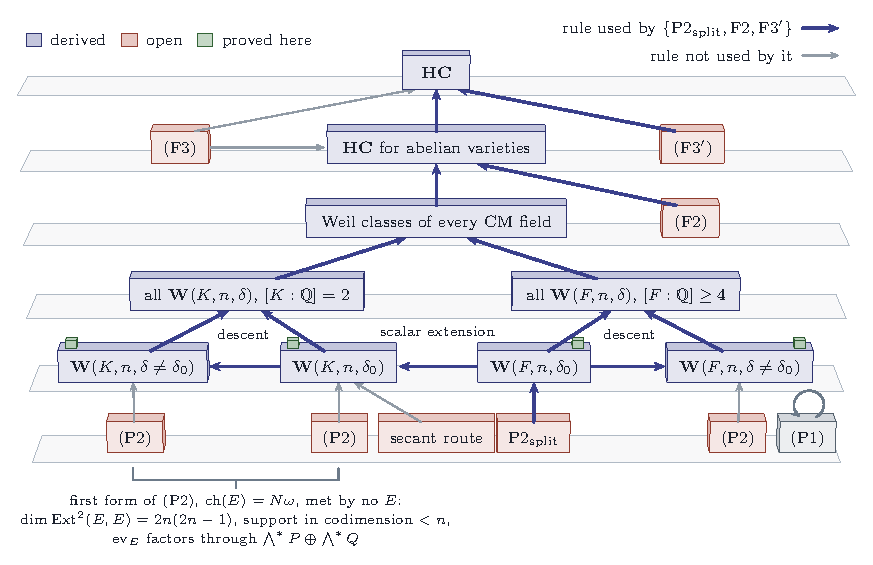
\includegraphics[width=\textwidth]{fig_closure}
\caption{The route of this paper through the rule set of \Cref{thm:closure},
drawn as a stack of plates, one per level of the derivation; the other routes
are drawn in \Cref{fig:frontier}. Heavy arrows are the rules used by the
minimal set $\{\mathrm{P2}_{\mathrm{split}},\mathrm{F2},\mathrm{F3}'\}$,
light arrows the rules it does not use. The bottom plate carries the
propagation statement, read in the polarised form of \Cref{rem:p2prime},
once for each of the four kinds of Weil family, with the secant route beside
it. The small grass blocks on the next plate are the base points of
\Cref{thm:everyfamily} and \Cref{thm:cmbasepoint}, one in every family. The
three arrows inside that plate are \Cref{prop:descent}: descent from the
trivial discriminant to the others, and scalar extension from the fields of
degree at least four to the quadratic fields. With them (P2) is needed only
for the split families of the fields of higher degree, and the other three
(P2) blocks are not used. (F2) is the conjecture for the Hodge classes that
no Weil line reaches, and (F3) is the whole conjecture
(\Cref{prop:f3ishc}), so the route is minimal only with (F3) replaced by
\textup{(F3$'$)} of \Cref{def:f3prime}. The bracket under the two quadratic
(P2) blocks records the first form of the criterion, in which the Chern
character is exactly a Weil class, as \Cref{thm:p2numerical},
\Cref{thm:p2support} and \Cref{cor:hhfactor} describe it; by
\Cref{thm:p2false} that form is met by no complex. The secant route reaches
the trivial discriminant, since the member it is built on is split, and
through descent the rest of the quadratic case; it has no edge to the fields
of higher degree. The bounded criterion (P1) stands apart, closed on itself:
it is equivalent to its own conclusion.}
\label{fig:closure}
\end{figure}


\subsection{Routes from outside algebraic geometry}\label{ssec:outside}

By \Cref{prop:f2isab} and \Cref{prop:f3prime}(i), the two statements
\textup{(F2)} and \textup{(F3$'$)} are the two halves of the conjecture: the
conjecture for abelian varieties, and the conjecture modulo abelian varieties.
A route from another domain must therefore either produce algebraic cycles or
arrive at one of the hypotheses of \Cref{setup:rules}. This subsection
records what the routes most often proposed do. One of them, the analytic
route through positive currents, can be made exact: the conjecture is the
vanishing of an integrality gap in a mass minimisation problem whose real
version is solved, and positivity, which is what analysis sees first, cannot
distinguish an algebraic class from any other.

Throughout, $X$ is a smooth complex projective variety of dimension $n$, $h\in
H^{2}(X,\ZZ)$ is the class of an ample line bundle, $\omega_{h}$ is a K\"ahler
form with class $h$, and for $c\in H^{2p}(X,\QQ)$ we put
\[
  L_{h}(c)=\int_{X}c\cup\frac{h^{\,n-p}}{(n-p)!}\in\QQ .
\]
A real $(p,p)$-form is \emph{strongly positive} if at every point it is a
nonnegative combination of forms $\mathrm{i}\beta_{1}\wedge\bbar{\beta}_{1}
\wedge\cdots\wedge\mathrm{i}\beta_{p}\wedge\bbar{\beta}_{p}$ with $\beta_{j}$
of type $(1,0)$; the closed positive currents of bidegree $(p,p)$ are the
currents nonnegative on such forms of the complementary degree, and every
smooth closed strongly positive form is one \cite[Chapter~III]{Dem12}.

\begin{proposition}[Positivity is no test]\label{prop:positivitynotest}
For every class $\alpha\in H^{p,p}(X,\RR)$, $0\le p\le n$, there is an integer
$N$ such that $\alpha+Nh^{p}$ is the class of a smooth closed strongly positive
$(p,p)$-form. Consequently every real $(p,p)$-class becomes the class of a
closed positive current after the addition of a multiple of $h^{p}$, and, since
$h^{p}$ is algebraic, a Hodge class is algebraic if and only if the positive
class $\alpha+Nh^{p}$ is: no property of a class implied by positivity, or by
its being a limit of classes of effective cycles, separates the algebraic Hodge
classes from the others.
\end{proposition}

\begin{proof}
Let $V=T_{x}X$ with the hermitian form $\omega_{h}(x)$, and let
$\mathrm{SP}_{p}\subseteq\Lambda^{p,p}_{\RR}V^{\vee}$ be the closed convex cone
generated by the forms $\mathrm{i}^{p}\beta_{1}\wedge\bbar{\beta}_{1}\wedge\cdots
\wedge\beta_{p}\wedge\bbar{\beta}_{p}$. These forms span
$\Lambda^{p,p}_{\RR}V^{\vee}$, so $\mathrm{SP}_{p}$ has nonempty interior, and
$\omega_{h}(x)^{p}$ lies in that interior: in a unitary basis $dz_{1},\dots,
dz_{n}$ of $V^{\vee}$,
\[
  \omega_{h}^{p}=p!\sum_{|J|=p}\Bigl(\frac{\mathrm{i}}{2}\Bigr)^{p}
  dz_{J}\wedge d\bbar{z}_{J},
\]
and a generator $D=\mathrm{i}^{p}\beta_{1}\wedge\bbar{\beta}_{1}\wedge\cdots\wedge
\beta_{p}\wedge\bbar{\beta}_{p}$ equals $|\det B|^{2}\,2^{p}(\mathrm{i}/2)^{p}
dz_{1}\wedge d\bbar{z}_{1}\wedge\cdots\wedge dz_{p}\wedge d\bbar{z}_{p}$ after a
unitary change of coordinates taking the span of the $\beta_{j}$ to that of
$dz_{1},\dots,dz_{p}$, with $B$ the matrix of the $\beta_{j}$ in that basis;
so $\omega_{h}^{p}-\delta D\in\mathrm{SP}_{p}$ for $0<\delta\le p!/(2^{p}
|\det B|^{2})$. As every real $(p,p)$-form is a finite real combination of
generators, $\omega_{h}^{p}+\varepsilon\gamma\in\mathrm{SP}_{p}$ for every
$\gamma$ and all small $\varepsilon$, which is interiority. The cone, the form
$\omega_{h}(x)^{p}$ and the norm defined by $\omega_{h}(x)$ are carried into
each other by unitary frames, so the radius $r>0$ of a ball around
$\omega_{h}(x)^{p}$ contained in $\mathrm{SP}_{p}$ does not depend on $x$.
Represent $\alpha$ by a smooth closed real $(p,p)$-form $a$, for instance its
harmonic representative, and let $N\ge\max_{X}|a|/r$. Then
$a+N\omega_{h}^{p}=N(\omega_{h}^{p}+a/N)$ is strongly positive at every point,
closed, and represents $\alpha+Nh^{p}$. The remaining assertions follow, the
last because a class of the form $\alpha+Nh^{p}$ is positive for every $\alpha$.
\end{proof}

The proposition says what positivity cannot do. Demailly studied the cone of
closed positive currents against the conjecture and constructed extremal
closed strongly positive currents that are not integration currents on
analytic sets \cite{Dem82}, so extremality does not single out the algebraic
cycles either. What positivity can do is turn the conjecture into a
variational statement, and the statement is exact. It is the K\"ahler case of
a formulation that Harvey and Lawson give for every calibrated manifold
\cite[Section~6, Proposition~6.13 and Remarks~6.9 and~6.11]{HL09}; we state
it for the classes of this paper, with the effective representative that
\Cref{lem:cibig} supplies, and then apply it to the Mumford square. For a
closed integral current $T$ of dimension $2(n-p)$ on $X$, Wirtinger's
inequality \cite[1.8.2]{Fed69}, \cite{HK74}, \cite[II.3]{HL82} gives
\begin{equation}\label{eq:wirtinger}
  \mathbf{M}(T)\;\ge\;T\Bigl(\frac{\omega_{h}^{\,n-p}}{(n-p)!}\Bigr)
  \;=\;L_{h}(c),
\end{equation}
where $\mathbf{M}$ is the mass and $c\in H^{2p}(X,\ZZ)$ is the Poincar\'e dual
of the homology class of $T$, with equality if and only if the approximate
tangent plane of $T$ is a complex subspace, positively oriented, at
$\|T\|$-almost every point. The right side depends on $c$ alone.

\begin{lemma}[Complete intersection classes are big]\label{lem:cibig}
For every algebraic class $\beta\in H^{2p}(X,\QQ)$ there is an integer $M$ such
that $\beta+Mh^{p}$ is a positive rational combination of classes of
irreducible subvarieties of codimension $p$; so some positive integer multiple
of $\beta+Mh^{p}$ is the class of an effective algebraic cycle.
\end{lemma}

\begin{proof}
Replacing $h$ by a multiple, which changes $M$, we may assume $h$ very ample.
Let $Z\subseteq X$ be irreducible of codimension $p$, and let $d$ be such that
the ideal sheaf $I_{Z}(d)$ is globally generated. The base locus of the linear
system of divisors of degree $d$ containing $Z$ is exactly $Z$, so by Bertini
$p$ general members $D_{1},\dots,D_{p}$ of it meet properly away from $Z$.
Every component of $D_{1}\cap\cdots\cap D_{p}$ has codimension at most $p$;
a component not contained in $Z$ has codimension exactly $p$, because the
$D_{i}$ meet properly off $Z$, and a component contained in $Z$ has
codimension at least $p$ and so equals $Z$. The intersection is therefore the
union of $Z$ and a closed set $W'$ of pure codimension $p$. Hence $d^{p}h^{p}=[D_{1}]\cdots[D_{p}]=m[Z]+[W']$ with $m\ge1$ and
$W'$ effective \cite[Chapter~7]{Ful98}, and $h^{p}-\varepsilon[Z]$ is an
effective rational class for $0<\varepsilon\le m/d^{p}$. Write
$\beta=\sum_{i}n_{i}[Z_{i}]$ with $n_{i}\in\QQ$ and choose $\varepsilon_{i}$ for
each $Z_{i}$ with $n_{i}<0$; then for $M\ge\sum_{n_{i}<0}|n_{i}|/\varepsilon_{i}$
the class $\beta+Mh^{p}$ is $\sum_{n_{i}>0}n_{i}[Z_{i}]+\sum_{n_{i}<0}
(|n_{i}|/\varepsilon_{i})(h^{p}-\varepsilon_{i}[Z_{i}])+(M-\sum_{n_{i}<0}
|n_{i}|/\varepsilon_{i})h^{p}$, a positive rational combination of effective
classes, $h^{p}$ itself being the class of a complete intersection.
\end{proof}

\begin{theorem}[The conjecture as a mass gap]\label{thm:massgap}
Let $\alpha\in\Hdg^{p}(X)$ be a rational Hodge class.
\begin{enumerate}[label=\textup{(\roman*)},leftmargin=2.6em,itemsep=2pt]
\item Let $N\ge1$ be an integer with $N\alpha$ integral, let $M$ be an
  integer for which $\alpha+Mh^{p}$ is the class of a smooth closed strongly
  positive form, as every large $M$ is by \Cref{prop:positivitynotest}, and
  put $c=N(\alpha+Mh^{p})$. The minimum of the mass over closed real normal
  currents of dimension $2(n-p)$ in the class dual to $c$ is $L_{h}(c)$, and
  it is attained by a smooth strongly positive form. The minimum over closed
  integral currents in the same class exists and is at least $L_{h}(c)$.
\item The class $\alpha$ is algebraic if and only if there are integers
  $N\ge1$ and $M\ge0$, with $N\alpha$ integral, for which the minimum of the
  mass over closed integral currents in the class dual to $N(\alpha+Mh^{p})$
  equals $L_{h}(N(\alpha+Mh^{p}))$; and then every mass minimising integral
  current in that class is the integration current of an effective algebraic
  cycle.
\item Write $\|c\|_{\ZZ}$ for the minimum in \textup{(i)} over integral
  currents. By a theorem of Federer, recorded in this form by Harvey and
  Lawson \cite[Section~6]{HL09}, \cite{Fed69,Fed74}, $\lim_{k\to\infty}
  \|kc\|_{\ZZ}/k=L_{h}(c)$: the integrality gap closes asymptotically for
  every class. The class $\alpha$ is algebraic if and only if, for every
  sufficiently large $M$, the gap is closed at some finite $k$, that is,
  $\|kc\|_{\ZZ}=kL_{h}(c)$ for some $k\ge1$.
\end{enumerate}
In particular the conjecture for $X$ is the statement that for every rational
Hodge class the integrality gap of this problem vanishes for some $N$ and $M$;
\textup{(F2)} is that statement for abelian varieties. Teh and Yang give a
different sufficient condition in the same setting, through Lipschitz chains
that are closed for $d$ and $d^{c}$ with positive $(k,k)$-part
\cite[Theorem~4.2]{TY21}.
\end{theorem}

\begin{proof}
(i) The form $\omega_{h}^{n-p}/(n-p)!$ has comass one and calibrates exactly
the complex $2(n-p)$-planes, which is Wirtinger's inequality
\cite[1.8.2]{Fed69}; so every closed real normal current $S$ in the class has
$\mathbf{M}(S)\ge S(\omega_{h}^{n-p}/(n-p)!)=L_{h}(c)$. By
\Cref{prop:positivitynotest} the class is represented by a smooth closed
strongly positive form $a$, and for a strongly positive $(p,p)$-form the mass of
the current it defines is $\int_{X}a\wedge\omega_{h}^{n-p}/(n-p)!$, because a
strongly positive $2(n-p)$-vector is a nonnegative combination of complex unit
planes, each of mass one and calibrated. So the minimum over real currents is
$L_{h}(c)$ and $a$ attains it. Closed normal currents represent every real
homology class and closed integral currents every integral one
\cite[5.11]{FF60}, and by the compactness theorem of Federer and Fleming the
mass attains its minimum on the closed integral currents in a given class
\cite[9.6]{FF60}; the lower bound is \eqref{eq:wirtinger}.

(ii) If $\alpha$ is algebraic, \Cref{lem:cibig} gives $M$ and $N$ with
$N(\alpha+Mh^{p})=\sum_{j}n_{j}[V_{j}]$, $n_{j}\in\ZZ_{>0}$, $V_{j}$
irreducible of codimension $p$. The integration current $T=\sum_{j}n_{j}[V_{j}]$
is a closed locally integral current \cite[Theorem~3.1.1]{Kin71}, its tangent
planes are complex and positively oriented, so equality holds in
\eqref{eq:wirtinger} and $\mathbf{M}(T)=L_{h}(c)$ with $c=N(\alpha+Mh^{p})$.
Conversely let $T$ be a closed integral current in the class dual to $c$ with
$\mathbf{M}(T)=L_{h}(c)$, for instance a mass minimiser when the minimum is
$L_{h}(c)$. Equality in \eqref{eq:wirtinger} makes $T$ a closed locally
rectifiable current of bidimension $(n-p,n-p)$ which is positive, and by
King's theorem \cite[Theorem~5.2.1]{Kin71} such a current is a holomorphic
cycle $\sum_{j}n_{j}[V_{j}]$ with $n_{j}$ nonzero integers and $V_{j}$
irreducible analytic subvarieties of dimension $n-p$; positivity makes every
$n_{j}$ positive. (Harvey and Shiffman characterised the holomorphic chains
among closed rectifiable currents of bidimension $(n-p,n-p)$ without
positivity, under a hypothesis on the support that Alexander removed
\cite{HS74,Ale97}.) By Chow's theorem \cite[p.~167]{GH78} the $V_{j}$
are algebraic, so $c$ is the class of an effective algebraic cycle and $\alpha$
is algebraic. This is the argument of \cite[Proposition~6.13]{HL09}.

(iii) The limit is Federer's theorem on the real and integral masses of a
class, as stated in the final note of \cite[Section~6]{HL09}; with (i) the
limit is $L_{h}(c)$, since the real minimum is attained by a smooth form. If
the gap is closed at $k$, then (ii), applied with $kN$ in place of $N$, makes
$\alpha$ algebraic. Conversely, if $\alpha$ is algebraic, \Cref{lem:cibig}
gives $M_{0}$ such that $\alpha+M_{0}h^{p}$ is a positive rational
combination of classes of subvarieties; for $M\ge M_{0}$ so is
$\alpha+Mh^{p}$, since $h^{p}$ is the class of a complete intersection, and
some multiple $kc$ is the class of an effective cycle, whose integration
current attains the bound. For a fixed small $M$ the equivalence is not asserted, since it would
need an effective multiple of every algebraic class represented by a
strongly positive form, in codimension at least two. The last sentence of the
theorem is the definition of the conjecture for $X$, and \Cref{prop:f2isab}
for \textup{(F2)}.
\end{proof}

\begin{example}[The Mumford square]\label{ex:mumfordmass}
Let $Y=X\times X$ be the square of a Mumford fourfold at a very general point
of its curve, with the product principal polarisation $\theta_{Y}$, and let
$\omega$ be one of the two exceptional classes of \Cref{prop:mumfordproduct},
normalised in $H^{2}(X)\otimes H^{2}(X)$ with $a_{0}=0$ in the notation of
\Cref{setup:omegaa}, so that it corresponds to an endomorphism of $H^{2}(X)$
killing $\theta$ with image in the primitive part. Then
$L_{\theta_{Y}}(\omega)=0$: the pairing of $\omega$ with
$\theta_{Y}^{6}=\sum_{k}\binom6k\theta^{k}\otimes\theta^{6-k}$ sees only the
term $20\,\theta^{3}\otimes\theta^{3}$, and $\int_{X}x\cup\theta^{3}=0$ for
every primitive $x\in H^{2}(X)$. Also $L_{\theta_{Y}}(\theta_{Y}^{2})=8!/6!=56$,
and $4\theta_{Y}^{2}$ is the class of the complete intersection $D\cap D'$ of two
general members of $|2\theta_{Y}|$, a base point free system, whose integration
current has mass $224$. By \Cref{thm:massgap} and \Cref{cor:mumfordone}, the
Hodge conjecture for every member of the Mumford family, and with it
$B(W\times_{C}W)$, is equivalent to the following: for some integers
$N\ge1$ and $M\ge1$ with $N\omega$ integral, the class dual to
$N(M\theta_{Y}^{2}+\omega)$ contains an integral current of mass exactly
$56NM$; and any such current is an effective algebraic cycle representing the
class. For $M$ divisible by four the class $NM\theta_{Y}^{2}$ contains one,
$NM/4$ copies of $D\cap D'$, of mass $56NM$; so the question is whether the
perturbation by $N\omega$, which changes the Wirtinger bound by nothing, can
be absorbed without mass. By \Cref{thm:mumfordcm} the answer is yes at
every CM point of the curve, with integers $N$ and $M$ depending on the
point; and if the same $N$ and $M$ served at infinitely many CM points the
answer would be yes everywhere, by \Cref{cor:mumfordbounded}, because the
components of an effective cycle of degree $56NM$ have degree at most $56NM$
and the Hilbert polynomials of subvarieties of bounded degree form a finite
set.
\end{example}

\Cref{fig:massgap} draws the theorem and the example.

\begin{figure}[tbp]
\centering
  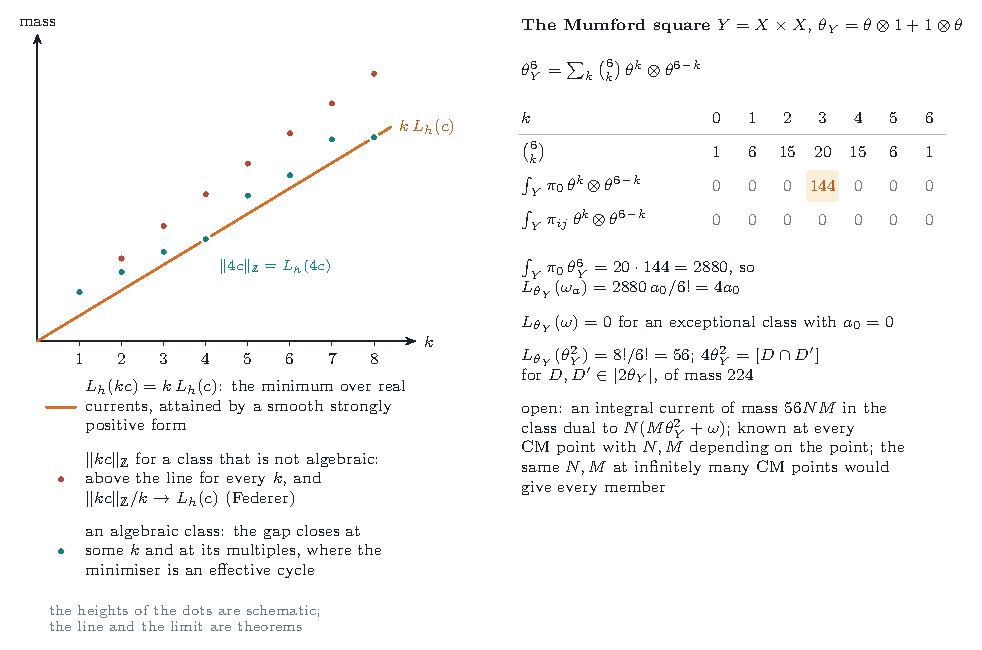
\includegraphics[width=\textwidth]{fig_massgap}
\caption{\Cref{thm:massgap} and \Cref{ex:mumfordmass}. Left: the mass of a
current in the class dual to $kc$ against $k$. The line $k\,L_{h}(c)$ is the
minimum over closed real normal currents, attained by a smooth strongly
positive form; the minima over closed integral currents lie on or above it,
with $\|kc\|_{\ZZ}/k\to L_{h}(c)$ by Federer's theorem, and for $M$ large the
class is algebraic exactly when one of them lies on the line, where the minimiser is
an effective algebraic cycle. The heights of the dots are schematic. Right:
the numbers of the Mumford square, in the split model. Of the seven terms $\binom6k\theta^{k}\otimes\theta^{6-k}$ of
$\theta_{Y}^{6}$ only $k=3$ pairs with $\pi_{0}=\frac14\theta\otimes\theta$,
giving $20\cdot144=2880$, and none pairs with the primitive summands; so
$L_{\theta_{Y}}(\omega_{a})=4a_{0}$, the Wirtinger bound of an exceptional
class with $a_{0}=0$ is zero, and the perturbation of $NM\theta_{Y}^{2}$ by
$N\omega$ changes the bound $56NM$ by nothing.}
\label{fig:massgap}
\end{figure}

\subsection{The routes at a glance}

\begingroup
\renewcommand{\arraystretch}{1.25}
\begin{longtable}{@{}>{\raggedright\arraybackslash}p{0.30\linewidth}>{\raggedright\arraybackslash}p{0.30\linewidth}>{\raggedright\arraybackslash}p{0.30\linewidth}@{}}
\caption{The routes considered, and the boundary of each result.}
\label{tab:scope}\\
\toprule
\textbf{Route} & \textbf{Result} & \textbf{Beyond the result} \\
\midrule
\endfirsthead
\multicolumn{3}{@{}l}{\footnotesize\itshape Table \thetable, continued.}\\[2pt]
\toprule
\textbf{Route} & \textbf{Result} & \textbf{Beyond the result} \\
\midrule
\endhead
\midrule
\multicolumn{3}{r@{}}{\footnotesize\itshape continued on the next page}\\
\endfoot
\bottomrule
\endlastfoot
Ambient object, restricted to $\Av$, transported by $\Phi_{\cP}$
  & closed by \Cref{thm:divisor}
  & ambient varieties with exceptional classes \\
Any $K$-equivariant construction with the norm character
  & closed by \Cref{thm:character}
  & constructions that are not eigenclasses \\
Secant dimension count
  & no obstruction, \Cref{cor:nonumerical}
  & none \\
Semiregularity dimension count
  & no obstruction, \Cref{cor:countnotbind}
  & none \\
Semiregularity of an object whose Chern character sits on the Weil line
  & closed by \Cref{thm:rankzero} and \Cref{cor:kernelfamily} for direct
    sums, and for every object by \Cref{thm:p2false}, for every CM field by
    \Cref{thm:cmpurefalse}
  & objects of positive rank; the weaker hypothesis of
    \cite[Question 11.4]{Mar25b} \\
The polarised criterion at a quartic CM field, $n=2$
  & computed for every shape, \Cref{thm:quarticrank}: a complex meeting it
    has $\dim\Ext^{2}(E,E)\ge88$, \Cref{cor:quarticleast}
  & existence of such a complex \\
Induction through hyperplane sections
  & closed by \Cref{thm:hyperplane}, \Cref{thm:returntrip}
  & correspondences, degenerations, coniveau \\
Kuga--Satake, from a weight two structure of K3 type
  & not obstructed, \Cref{prop:ksnotrestriction}
  & available only at $n=1$, \Cref{cor:ksboundary} \\
Divisors, on a member with quaternionic multiplication
  & succeeds, \Cref{thm:quatweil}
  & fails at full Hodge group, \Cref{prop:divfails} \\
Propagation off the base locus
  & reduced to one bound or one rank, \Cref{thm:degreebound},
    \Cref{thm:semiregclosure}
  & the bound or the rank, \Cref{rem:tworemain} \\
Objects with effective Chern character at a base point
  & closed by \Cref{thm:positivity}
  & objects indecomposable in $D^{b}$, \Cref{rem:whatitmustbe} \\
The weakened criterion for a secant object of positive rank
  & reduced to two conditions on the factor, \Cref{thm:factor}, the first
    automatic for Markman's construction, \Cref{cor:markmancondition}; the
    identity fails for Markman's candidate, \Cref{thm:candidatefails}, and at every
    transversal double point, \Cref{cor:localobstruction}
  & objects whose support has no such point, \Cref{rem:candidatemeaning} \\
A secant object $\cI_{S}(b\Theta)$ with smooth support
  & invariants forced and $d\le b^{2}$, so $d\le9$ at $b=3$,
    \Cref{thm:smoothinvariants}, \Cref{cor:fourdiscriminants}
  & existence for $d\in\{1,3,5,7\}$ at $b=3$, one vanishing in
    $H^{1}(S,N_{S/X})$ and first-order extension, \Cref{rem:smoothremains} \\
The local part of the weakened criterion
  & it is a condition on depth: no obstruction at a Cohen--Macaulay point,
    \Cref{thm:cmvanishing}, \Cref{cor:cmdichotomy}
  & Cohen--Macaulay supports, where the identity becomes one global
    vanishing beside first-order extension \\
A support that is a complete intersection
  & closed for every $b$ and every $d$, \Cref{thm:noci}
  & supports of higher Hilbert--Burch rank, \Cref{prop:lowrankburch} \\
A support with a Hilbert--Burch resolution by line bundles or by simple
semi-homogeneous bundles
  & closed for every rank, twist and $d$, \Cref{thm:nosplit},
    \Cref{thm:noblocks}
  & resolutions over bundles that are not projectively flat \\
The secant route, granted every demand it makes
  & reaches $\delta=\delta_{0}$, and every $\delta$ by \Cref{prop:descent},
    \Cref{thm:closure}(iv)
  & the CM fields of degree at least four, which give the quadratic ones by
    \Cref{prop:descent}(ii) \\
Propagation from a base point
  & closes every imaginary quadratic family at once, \Cref{thm:degreebound},
    \Cref{thm:semiregclosure}
  & (P2) for the family, \Cref{cor:fourremain} \\
The bounded form (P1), read on the transported cycle
  & closed: the transport spreads each component by $c^{2n}/m_{i}$ and the
    data is unbounded whenever a component has finite stabiliser,
    \Cref{lem:multiplicity}, \Cref{thm:p1forces}
  & nothing; the other reading is closed too \\
The bounded form (P1), read on the minimal representative
  & closed: equivalent to the conjecture for the family,
    \Cref{thm:p1equivalent}
  & nothing; it is a restatement, so it is not a route \\
The pure form of (P2), for a given representative
  & forces the evaluation map to vanish on the $4n^{2}$-dimensional
    annihilator, and excludes every representative that is a sheaf on a
    smooth germ of codimension two of its support, \Cref{thm:p2forces},
    \Cref{cor:p2shape}
  & nothing: no representative exists, \Cref{thm:p2false} \\
The same form, tested by a number
  & $\dim\Ext^{2}(E,E)=2n(2n-1)$ at one base point would suffice,
    \Cref{thm:p2numerical}, and no representative attains it,
    \Cref{thm:p2false}
  & nothing \\
The same form, for a representative in codimension $n$
  & closed at every member of every family: the support must have a
    component of codimension less than $n$, and at a general member every
    component of codimension at least two has multiplicity zero,
    \Cref{lem:finiteproduct}, \Cref{thm:p2support}
  & nothing: no representative exists, \Cref{thm:p2false} \\
The Hochschild action on such a representative
  & the annihilator is the mixed part of a splitting of $HH^{1}$ and the
    action factors through a ring of dimension $2^{2n+1}-1$ in one of
    dimension $2^{4n}$, \Cref{thm:hhsplitting}, \Cref{cor:hhfactor}
  & nothing: no such complex exists, \Cref{thm:p2false} \\
The shape of such a representative
  & an indecomposable summand carries the class; at $n=2$, and at $n=3$
    granting the compatibility of \Cref{cor:hhfactor}(iii), its
    endomorphism algebra has dimension at least three, so no simple object
    serves, \Cref{thm:p2endo}
  & nothing: no object of any shape meets the pure form, \Cref{thm:p2false} \\
The pure form of (P2), Chern character exactly a Weil class
  & false for every imaginary quadratic field and every $n\ge2$: a
    semiregular such complex would deform to very general non-algebraic Weil
    tori, whose coherent sheaves have no Chern character below the top
    degree, \Cref{prop:weiltorussheaves}, \Cref{thm:p2false}
  & the polarised form (P2$'$), whose Chern character may carry powers of
    the polarisation, \Cref{rem:p2prime} \\
The reduction to Weil classes, and to abelian varieties
  & false as a statement about Hodge rings in dimension eight,
    \Cref{prop:mumfordproduct}; impossible Hodge-theoretically,
    \Cref{prop:noabeliantype}
  & the algebraicity of the classes beyond the Weil lines, which is (F2), and
    (F3), which is the whole conjecture, \Cref{prop:f3ishc} \\
The two classes on the self-product of a Mumford fourfold
  & a real multiplication by a cubic field on the primitive part of $H^{2}$,
    algebraic once the Kuga--Satake class of one K3 surface of Picard number
    thirteen is, \Cref{prop:mumfordrm}, \Cref{thm:mumfordks}
  & that Kuga--Satake class, \Cref{rem:mumfordks} \\
Other routes to the same two classes
  & degeneration and larger families closed off by rigidity; semiregularity
    reduced to $\dim\Ext^{2}=119$ at one CM point; specialisation reduced to
    a degree bound, \Cref{thm:mumfordrigid}, \Cref{thm:mumfordnumerical},
    \Cref{cor:mumfordbounded}
  & an object with $\dim\Ext^{2}=119$, or the degree bound,
    \Cref{rem:bypassaudit} \\
The cycles at a CM point, for the same two classes
  & the fourfold is of Weil type for $k_{c}\subset\End^{0}(X_{c})$ with the
    two exotic classes as its Weil line; pull-backs of that line along
    homomorphisms with components in $k_{c}$ span, with divisor products,
    $110$ of the $132$ Hodge classes of the square and no exceptional class,
    and an exceptional class is reached exactly by components generating the
    endomorphism algebra over $k_{c}$, \Cref{prop:cmsource}
  & a degree bound for cycles using the real multiplication, at infinitely
    many CM points, \Cref{rem:cmsource} \\
Objects built from line bundles, for the same two classes
  & closed at every point of the curve: the Chern characters stay invariant
    under the Lefschetz group, \Cref{thm:lefschetzclosure}
  & steps that break that symmetry, \Cref{rem:leavel} \\
Twistor deformation of the square, for the same two classes
  & closed: the component of the Hodge locus among all complex tori is the
    Mumford curve, which contains no twistor line, \Cref{prop:notwistor}
  & the Kuga--Satake class, which moves in a seven-dimensional family \\
Five further routes, for the same two classes
  & one statement: three of them are equivalent to the target and two imply
    it, so any one of them suffices, \Cref{cor:mumfordone}
  & the target itself, which is only the first case of (F2),
    \Cref{rem:mumfordneeded} \\
Pull-back from a hyperk\"ahler manifold, for the same two classes
  & the square is holomorphic symplectic and the classes are the twisted dual
    forms of the part of $H^{2}$ its symplectic class generates; a symplectic
    rational map to some $S_{\mu}^{[n]}$, $n\ge5$, suffices, and no K3
    surface or hyperk\"ahler eightfold serves, \Cref{prop:hksquare}
  & such a map, \Cref{rem:hkroute} \\
Reduction modulo $p$, for the same two classes
  & represented by cycles at every closed point of every reduction; the
    target is equivalent to a bound on their Hilbert data on a Zariski dense
    set, \Cref{prop:modp}, \Cref{thm:modpdensity}
  & the bound, \Cref{rem:modpremains} \\
The Weil classes of every CM field
  & the same propagation problem, with a CM base point in every family,
    \Cref{thm:cmbasepoint}, \Cref{thm:cmpropagation}
  & (P2) for the split families \\
Routes from outside algebraic geometry
  & positivity of currents sees nothing; the conjecture is the vanishing of
    the integrality gap of a mass minimisation whose real version is solved,
    \Cref{prop:positivitynotest}, \Cref{thm:massgap}
  & a calibrated integral current in one class, \Cref{ex:mumfordmass} \\
The closure, as a whole
  & five minimal sets of hypotheses: $\{\mathrm{F3}\}$ and
    $\{\mathrm{L},\mathrm{M}\}$, each equivalent to the conjecture, and
    three through the conjecture modulo abelian varieties,
    $\{\mathrm{L},\mathrm{F3}'\}$, $\{\mathrm{V},\mathrm{F3}'\}$ and this
    route, $\{\mathrm{P2}_{\mathrm{split}},\mathrm{F2},\mathrm{F3}'\}$,
    \Cref{thm:closure}, \Cref{prop:f3ishc}, \Cref{cor:fourremain},
    \Cref{rem:bullseye}
  & the Lefschetz standard conjecture, (M), (V), (F2), (F3$'$) \\
Convolutions of the Weil pieces on $E_{0}^{2n}$
  & at $n=3$ every convolution has $\dim\Ext^{2}\ge69>57$,
    \Cref{thm:noconvolution}; at $n=4$, with the pieces at two shifts,
    $\dim\Ext^{2}\ge40960>104$, \Cref{thm:efourtwolevels}, at three
    consecutive shifts $\dim\Ext^{2}\ge22528$, \Cref{thm:efourthreelevels},
    with the shifts within six consecutive values $\dim\Ext^{2}\ge640$,
    \Cref{cor:efoursix}, and with each parity at one shift, at any odd
    distance, $\dim\Ext^{2}\ge1792$, \Cref{prop:efoursingle}
  & the other arrangements of the shifts at $n=4$,
    \Cref{rem:convolutionsopen} \\
Diagonal complete intersections of Vandermonde type
  & quotients of powers of a generalised Fermat curve, so in $\mathcal{A}$;
    the conjecture holds when it holds on the abelian varieties $B_{[a]}$, and
    holds for two diagonal hypersurfaces of degree $3$, $4$, $6$ in
    $\PP^{6}$, \Cref{thm:vandermonde}, \Cref{cor:twodiagonal}; it holds on
    the very general member for $d=2$ in every dimension, for $d=3,4$ up
    to dimension seven and for $d=6$ up to dimension five,
    \Cref{thm:vgvandermonde}
  & $B_{[a]}$ of dimension above five, the Weil classes of
    $\QQ(\zeta_{e})$ with $\varphi(e)\ge4$, and the very general member
    for $d=3,4,6$ from dimension eight on and for $d=6$ in dimension six,
    \Cref{rem:vandermonde} \\
The conjecture modulo abelian varieties, (F3$'$)
  & holds on the class $\mathcal{A}$ of varieties whose cohomology is
    reached from abelian varieties by algebraic correspondences (curves,
    abelian varieties, products, surjective images), in degrees $0$, $2$,
    $2n-2$, $2n$, and in dimension at most three, \Cref{prop:f3prime};
    on the Delsarte hypersurfaces and the diagonal complete intersections
    of Vandermonde type, \Cref{cor:delsarteall}, \Cref{thm:vandermonde};
    on the fourfolds and fivefolds of \Cref{prop:f3primesmall},
    \Cref{prop:f3primefibration} and \Cref{prop:f3primedominant};
    through the Hodge conjecture on the varieties of \Cref{prop:k3powers}
    and \Cref{prop:k3ntype}
  & degree four on fourfolds outside $\mathcal{A}$ not covered by these
    results, and beyond, for
    instance squares of K3 surfaces with real multiplication, such as
    $S_{\lambda}$, \Cref{rem:f3primeopen},
    \Cref{rem:f3primefrontier} \\
\end{longtable}
\endgroup

\section{Hodge classes beyond the Weil lines}\label{sec:beyond}

\subsection{The first classes beyond the Weil lines}\label{ssec:mumford}

Statement (F2) is the Hodge conjecture for the Hodge classes on abelian
varieties that no Weil line reaches, and \Cref{prop:mumfordproduct} exhibits
the first of them: two classes in $H^{4}(X\times X,\QQ)$ for an abelian
fourfold $X$ of Mumford type. None of the constructions of the preceding
sections acts on them. In this subsection we identify them as a real
multiplication on the primitive part of $H^{2}(X)$, and we prove that they
are algebraic as soon as the Kuga--Satake class of one K3 surface of Picard
number thirteen attached to $X$ is algebraic. We do not prove that the
Kuga--Satake class is algebraic, and we know of no proof. The reduction
changes the kind of question: two classes on an eightfold are traded for one
correspondence of a well-studied type, between a surface and its Kuga--Satake
variety. The cubic field of the real multiplication enters through the
Clifford relations, which force the blocks of the Kuga--Satake embedding to
span it.

\begin{setupenv}[Mumford type]\label{setup:mumford}
Let $X$ be as in \Cref{prop:mumfordproduct}, with $V=H^{1}(X,\QQ)$,
polarisation $\psi$ and polarisation class $\theta\in H^{2}(X,\QQ)$, and let
$G=\Hg(X)$. Over $\bar{\QQ}$ the Hodge cocharacter is nontrivial on exactly
one of the three factors of $G$: on $V_{i}$ it has weights $\pm a_{i}/2$ with
$a_{i}\ge0$, and $V$ has only the two weights $\pm\frac12$, so exactly one
$a_{i}$ is nonzero. Since $\End^{0}(X)=\QQ$, it follows that $G$ is
$\QQ$-simple: the Lie algebra of a $\QQ$-factor not containing that geometric
factor would consist of Hodge classes in $\End(V)$, that is, of endomorphisms
of $X$. So $G$ is the image in
$\GL(V)$ of $\Res_{F/\QQ}D^{1}$, where $F$ is a totally real cubic field, $D$
is a quaternion algebra over $F$ split at one real place $\sigma_{3}$ and
definite at the other two, $\sigma_{1}$ and $\sigma_{2}$, with
$\operatorname{Cor}_{F/\QQ}D\cong M_{8}(\QQ)$, and $D^{1}$ is the group of
elements of reduced norm one \cite{Mum69,Gal00}; the kernel is the central
subgroup of triples of signs with product one. Over $\bar{\QQ}$,
$V=V_{1}\otimes V_{2}\otimes V_{3}$, where $V_{i}$ is the standard
representation of $D\otimes_{F,\sigma_{i}}\bar{\QQ}=M_{2}(\bar{\QQ})$; the
Galois group permutes the three factors as it permutes the three embeddings,
and $H^{1,0}(X)=V_{1}\otimes V_{2}\otimes V_{3}^{1,0}$. Put
\[
  T=\operatorname{Lie}G=D^{0},
  \qquad
  q_{\lambda}(x,y)=\Tr_{F/\QQ}\bigl(\lambda\operatorname{trd}(xy)\bigr)
  \quad(\lambda\in F^{\times}),
\]
where $D^{0}$ is the space of quaternions of reduced trace zero, regarded as
a $\QQ$-vector space of dimension nine, and $\operatorname{trd}$ is the
reduced trace. Over $\bar{\QQ}$, $T=T_{1}\oplus T_{2}\oplus T_{3}$ with
$T_{i}=\mathfrak{sl}(V_{i})$, and $a\in F$ acts on $T_{i}$ by $\sigma_{i}(a)$.
Write $m_{a}$ for multiplication by $a$. The space $T\subset\End(V)$ is a
sub-Hodge structure of weight zero.
\end{setupenv}

\begin{proposition}[The two classes are a real multiplication]%
\label{prop:mumfordrm}
In \Cref{setup:mumford}:
\begin{enumerate}[label=\textup{(\roman*)},nosep,leftmargin=2.6em]
\item $H^{2}(X,\QQ)=\QQ\theta\oplus U$, where $U$ is the primitive part, of
  dimension $27$, and over $\bar{\QQ}$
  \[
    U=U_{12}\oplus U_{13}\oplus U_{23},\qquad
    U_{ij}=S^{2}V_{i}\otimes S^{2}V_{j}\otimes{\textstyle\bigwedge^{2}}V_{k},
    \quad \{i,j,k\}=\{1,2,3\},
  \]
  each of dimension nine. The summand $U_{12}$ is of type $(1,1)$, and
  $U_{13}$ and $U_{23}$ have Hodge numbers $(3,3,3)$.
\item The algebra of Hodge endomorphisms of $H^{2}(X,\QQ)$ is $\QQ\times F$,
  acting by scalars on $\QQ\theta$, with $a\in F$ acting on $U_{ij}$ by
  $\sigma_{k}(a)$. Through Poincar\'e duality and the Lefschetz isomorphism
  $\theta^{2}\colon H^{2}\to H^{6}$ this algebra is the space of Hodge classes
  in the K\"unneth component $H^{2}(X)\otimes H^{2}(X)$ of
  $H^{4}(X\times X,\QQ)$; the subalgebra $\QQ\times\QQ$ is spanned by the
  products of divisor classes that lie there, and the two classes of
  \Cref{prop:mumfordproduct}(ii) may be taken to be the elements of $F$ of
  trace zero.
\item $T(-1)$ is a Hodge structure of K3 type with Hodge numbers $(1,7,1)$,
  and its Hodge endomorphisms are the $m_{a}$, $a\in F$. The $G$-invariant
  symmetric forms on $T$ are the $q_{\lambda}$, and $q_{\lambda}$ polarises
  $T(-1)$ if and only if $\lambda$ is totally positive.
\end{enumerate}
\end{proposition}

\begin{proof}
(i) is the decomposition of $\bigwedge^{2}(V_{1}\otimes V_{2}\otimes V_{3})$
in the proof of \Cref{prop:mumfordproduct}, where $U_{ij}$ appears as the
summand of highest weight $2$ on the $i$-th and $j$-th factors. The Hodge
cocharacter acts trivially on $V_{1}$ and $V_{2}$ and splits
$V_{3}=V_{3}^{1,0}\oplus V_{3}^{0,1}$, so $\bigwedge^{2}V_{3}$ has type
$(1,1)$ and $S^{2}V_{3}$ has one dimension of each of the types $(2,0)$,
$(1,1)$, $(0,2)$.

(ii) A Hodge endomorphism commutes with the Mumford--Tate group
$G\cdot\mathbb{G}_{m}$, and $\mathbb{G}_{m}$ acts on $H^{2}$ by scalars, so
the Hodge endomorphisms are the $G$-endomorphisms. Over $\bar{\QQ}$ the four
summands $\QQ\theta$, $U_{12}$, $U_{13}$, $U_{23}$ are irreducible and
pairwise non-isomorphic, so the $G$-endomorphisms are the combinations of the
four projections. The Galois group fixes the projection onto $\QQ\theta$ and
permutes the other three as it permutes the indices $k$, that is, as it
permutes the embeddings of $F$. For $a\in F$ an endomorphism acting on
$U_{ij}$ by $\sigma_{k}(a)$ is therefore Galois invariant, hence rational, and
with the scalars on $\QQ\theta$ these exhaust the rational points, which form
$\QQ\times F$. Poincar\'e duality identifies $\End H^{2}(X,\QQ)$ with
$H^{6}(X)\otimes H^{2}(X)$, and $\theta^{2}\otimes1$ carries
$H^{2}\otimes H^{2}$ onto it; both are given by algebraic classes, and on an
abelian variety so is the inverse of the Lefschetz isomorphism
\cite[\S2]{Kle68}. The products of divisor classes in $H^{2}\otimes H^{2}$
are $\psi_{11}\psi_{22}$ and $\psi_{12}^{2}$ in the notation of the proof of
\Cref{prop:mumfordproduct}. They are invariant under the whole of
$\Sp(V,\psi)$, whose endomorphisms of $H^{2}=\QQ\theta\oplus U$ are spanned
by the identity and the projection onto $\QQ\theta$, and they are linearly
independent, being a multiple of the projection and a multiple of the
identity (proof of \Cref{prop:mumfordproduct}); so they span $\QQ\times\QQ$, and any complement of
$\QQ\times\QQ$ in $\QQ\times F$ may serve as the two remaining classes.

(iii) The adjoint action of the Hodge cocharacter is trivial on $T_{1}$ and
$T_{2}$ and has weights $-1$, $0$, $1$ on $T_{3}$, so $T$ has Hodge numbers
$(1,7,1)$ in the types $(-1,1)$, $(0,0)$, $(1,-1)$, and $T(-1)$ is of K3
type. Its Hodge endomorphisms are again the $G$-endomorphisms, and the
argument of (ii), applied to the three pairwise non-isomorphic summands
$T_{i}$, gives $F$ acting by multiplication. On each $T_{i}$ the invariant
symmetric forms are the multiples of $\operatorname{tr}(xy)$, and
$\operatorname{tr}(x_{i}y_{i})=\sigma_{i}(\operatorname{trd}(xy))$ for
$x,y\in D^{0}$, so the Galois-invariant ones are the $q_{\lambda}$. At
$\sigma_{1}$ and $\sigma_{2}$ the algebra $D\otimes\RR$ is Hamilton's
quaternions, $T_{i}$ is of type $(1,1)$, and
$\operatorname{trd}(x^{2})=-2\operatorname{nrd}(x)$ is negative on nonzero
pure quaternions. At $\sigma_{3}$ the form
$\operatorname{tr}(xy)$ on $\mathfrak{sl}_{2}(\RR)$ is negative on the line of
type $(1,1)$, the Lie algebra of the rotations fixed by the Hodge
cocharacter, and positive on its orthogonal complement, the real points of
the types $(2,0)$ and $(0,2)$. The Hodge--Riemann relations for a structure
of K3 type ask for exactly these signs after multiplication by
$\sigma_{i}(\lambda)$, so $q_{\lambda}$ polarises $T(-1)$ precisely when every
$\sigma_{i}(\lambda)$ is positive.
\end{proof}

The two classes are thus the endomorphisms of $U$ given by the elements of
$F$ of trace zero. A Hodge structure of K3 type with the same field sits
beside them, and the next lemma connects the two.

\begin{lemma}[The product map]\label{lem:mumfordmu}
For $x,y\in T$ let $\mu(x\otimes y)\in H^{2}(X,\QQ)$ be the class that
corresponds under $\psi$ to the alternating form
$(v,w)\mapsto\psi(xv,yw)+\psi(yv,xw)$ on $V$. Then $\mu$ is a $G$-equivariant
map $T\otimes T\to H^{2}(X,\QQ)$, and:
\begin{enumerate}[label=\textup{(\roman*)},nosep,leftmargin=2.6em]
\item for $i\ne j$ it restricts to an isomorphism $T_{i}\otimes T_{j}\to
  U_{ij}$, and it carries $T_{i}\otimes T_{i}$ onto $\QQ\theta$;
\item for $e,\lambda\in F^{\times}$ put $\mu_{e}=\mu\circ(m_{e}\otimes m_{e})$
  and let $\mu_{e}^{\dagger}$ be its adjoint for the form
  $q_{\lambda}\otimes q_{\lambda}$ on $T\otimes T$ and the Lefschetz pairing
  $B(\alpha,\beta)=\int_{X}\alpha\beta\,\theta^{2}$ on $H^{2}(X,\QQ)$. Then
  $\mu_{e}\mu_{e}^{\dagger}$ preserves $\QQ\theta$ and acts on $U$ as the
  element
  \[
    \nu\,\Nm_{F/\QQ}(g)\,g^{-1}\in F,\qquad g=e^{2}/\lambda,
  \]
  where $\nu$ is a nonzero rational number independent of $e$ and $\lambda$.
\end{enumerate}
\end{lemma}

\begin{proof}
Equivariance is clear, since $\mu$ is built from $\psi$ and the action of
$\End(V)$ on $V$. An element $x\in T_{i}$ acts on $V$ through the $i$-th factor
and lies in the symplectic Lie algebra of $\psi=\epsilon_{1}\otimes
\epsilon_{2}\otimes\epsilon_{3}$, so $\psi(xv,yw)=-\psi(v,xyw)$ and
$\mu(x\otimes y)$ is the form $-\psi(v,(xy+yx)w)$. If $x\in T_{i}$ and
$y\in T_{j}$ with $i\ne j$, then $xy=yx$ acts as $x\otimes y$ on
$V_{i}\otimes V_{j}$, and the form is $-2$ times the product of
$\epsilon_{i}(\cdot,x\,\cdot)$, $\epsilon_{j}(\cdot,y\,\cdot)$ and
$\epsilon_{k}$; the first two are symmetric because $x$ and $y$ lie in
$\mathfrak{sp}(\epsilon)=\mathfrak{sl}_{2}$, and $x\mapsto\epsilon(\cdot,x\,\cdot)$
is an isomorphism $\mathfrak{sl}_{2}\to S^{2}V^{\vee}$, so $\mu$ maps
$T_{i}\otimes T_{j}$ isomorphically onto $U_{ij}$. If $i=j$, then
$xy+yx=\operatorname{tr}(xy)$ on $V_{i}$, because $x$ and $y$ are trace-free
$2\times2$ matrices, and $\mu(x\otimes y)=-\operatorname{tr}(xy)\,\theta$.

For (ii), $m_{e}$ is self-adjoint for $q_{\lambda}$, and the adjoint of a
map out of $(T\otimes T,q_{\lambda}\otimes q_{\lambda})$ is
$(m_{\lambda}\otimes m_{\lambda})^{-1}$ times its adjoint for
$q_{1}\otimes q_{1}$, so
$\mu_{e}\mu_{e}^{\dagger}=\mu\,(m_{g}\otimes m_{g})\,\mu^{\dagger_{1}}$ with
$\mu^{\dagger_{1}}$ the adjoint for $q_{1}\otimes q_{1}$. This map is
$G$-equivariant, so it preserves $\QQ\theta$ and each $U_{ij}$, and
$\mu^{\dagger_{1}}$ carries $U_{ij}$ into
$(T_{i}\otimes T_{j})\oplus(T_{j}\otimes T_{i})$, on which $m_{g}\otimes m_{g}$
is multiplication by $\sigma_{i}(g)\sigma_{j}(g)=\Nm(g)/\sigma_{k}(g)$. Hence
$\mu_{e}\mu_{e}^{\dagger}$ is $\Nm(g)\sigma_{k}(g)^{-1}$ times
$\mu\mu^{\dagger_{1}}$ on $U_{ij}$. The summands of $H^{2}(X,\bar{\QQ})$ are
pairwise non-isomorphic and self-dual, so $B$ is nondegenerate on $U_{ij}$,
and by Schur's lemma the pull-back of $B$ along the isomorphism
$\mu_{0}=\mu|_{T_{i}\otimes T_{j}}$ is $c_{k}\,q_{1}\otimes q_{1}$ with
$c_{k}\ne0$; then $\mu_{0}\mu_{0}^{\dagger_{1}}=c_{k}$ on $U_{ij}$. As $\mu$
is symmetric in its two arguments and the exchange of the factors is an
isometry of $q_{1}\otimes q_{1}$, $\mu^{\dagger_{1}}u=\mu_{0}^{\dagger_{1}}u+
s\,\mu_{0}^{\dagger_{1}}u$ with $s$ that exchange, and $\mu\mu^{\dagger_{1}}=2c_{k}$
on $U_{ij}$. On the split model $V=\bar{\QQ}^{2}\otimes\bar{\QQ}^{2}\otimes
\bar{\QQ}^{2}$, $\psi=\epsilon\otimes\epsilon\otimes\epsilon$, the
permutations of the three factors preserve $\psi$, hence $\theta$, $B$ and
$\mu$, and also $q_{1}=\sum_{i}\operatorname{tr}(x_{i}y_{i})$, while they
permute the $U_{ij}$; so $c_{1}=c_{2}=c_{3}$, and $\mu\mu^{\dagger_{1}}$ is one
and the same nonzero number $\nu$ on the three summands $U_{ij}$, rational
because $\mu\mu^{\dagger_{1}}$ is defined over $\QQ$. By \Cref{prop:mumfordrm}(ii) an endomorphism of $U$ acting
on $U_{ij}$ by $\nu\Nm(g)/\sigma_{k}(g)$ is the element $\nu\Nm(g)g^{-1}$ of
$F$.
\end{proof}

\Cref{fig:mumford} draws \Cref{prop:mumfordrm} and \Cref{lem:mumfordmu} over
the three factors of the Hodge group.

By the Kuga--Satake class of a projective K3 surface $S$ we mean the Hodge
class on $S\times\mathrm{KS}(S)\times\mathrm{KS}(S)$ that induces the embedding
of \Cref{prop:ksembed} for $T(S)_{\QQ}$; its algebraicity is the Kuga--Satake
Hodge conjecture for $S$ (\Cref{rem:kstransport}).

\begin{theorem}[One K3 surface for the two classes]\label{thm:mumfordks}
In \Cref{setup:mumford}, let $\lambda\in F$ be totally positive.
\begin{enumerate}[label=\textup{(\roman*)},nosep,leftmargin=2.6em]
\item There is a projective K3 surface $S_{\lambda}$ of Picard number
  thirteen and an isomorphism of Hodge structures
  $T(S_{\lambda})_{\QQ}\cong T(-1)$ carrying the intersection form to
  $q_{\lambda}$. Its Kuga--Satake variety is isogenous to $X^{32}$.
\item If the Kuga--Satake class of $S_{\lambda}$ is algebraic, then the real
  multiplication by $F$ on $T(S_{\lambda})$ is induced by algebraic cycles on
  $S_{\lambda}\times S_{\lambda}$, and every Hodge class in
  $H^{4}(X\times X,\QQ)$ is algebraic; in particular the two classes of
  \Cref{prop:mumfordproduct}(ii) are algebraic.
\end{enumerate}
\end{theorem}

\begin{proof}
(i) The quadratic space $(T,q_{\lambda})$ has dimension nine and signature
$(2,7)$ by \Cref{prop:mumfordrm}(iii), and $H^{2}$ of a K3 surface with its
intersection form has dimension $22$ and signature $(3,19)$. Over $\QQ_{p}$
a nondegenerate quadratic space embeds isometrically in every nondegenerate
space of dimension at least three larger, and over $\RR$ the signatures
allow it, so by the Hasse--Minkowski theorem for representations of forms by
forms \cite[\S\S63, 66]{OMe00} there is an isometric embedding of
$(T,q_{\lambda})$ into $\Lambda_{\QQ}$, where $\Lambda$ is the K3 lattice.
The line $\ell=T(-1)^{2,0}\subset T_{\CC}\subset\Lambda_{\CC}$ satisfies
$(\ell,\ell)=0$ and $(\sigma,\bar{\sigma})>0$ for $0\ne\sigma\in\ell$, so by the
surjectivity of the period map there is a K3 surface $S_{\lambda}$ with a
marking $H^{2}(S_{\lambda},\ZZ)\cong\Lambda$ that carries
$H^{2,0}(S_{\lambda})$ to $\ell$ \cite[Chs.~6--7]{Huy16}. A rational class
is of type $(1,1)$ exactly when it is orthogonal to $\ell$, and its component
in $T$ is then a rational class of type $(1,1)$ in $T(-1)$, that is a
$G$-invariant vector of $T=\operatorname{Lie}G$; there is none, since $G$ is
semisimple. So $\NS(S_{\lambda})_{\QQ}=T^{\perp}$, of dimension $13$ and
signature $(1,12)$, and $T(S_{\lambda})_{\QQ}=T$ with the form $q_{\lambda}$.
A class of positive square in $\NS(S_{\lambda})$ makes $S_{\lambda}$
projective \cite[Ch.~8]{Huy16}.

For the Kuga--Satake variety, note first that over $\bar{\QQ}$ the space $T$
is the orthogonal sum of the three ternary spaces $T_{i}$, so $C(T)$ is the
graded tensor product of the $C(T_{i})$. Scaling a ternary form does not
change its even Clifford algebra, so $D^{1}$ is the spin group of
$(D^{0},\lambda\operatorname{trd})$ for every $\lambda$, and
$\Res_{F/\QQ}D^{1}$ maps to $\mathrm{Spin}(T,q_{\lambda})$ by multiplication
in the Clifford algebra, with the same kernel as its map to $\GL(V)$, so that
$G$ is a subgroup of $\mathrm{Spin}(T,q_{\lambda})$; as a representation of
the $i$-th factor, $C(T_{i})$ is four copies of $V_{i}$. Hence $C^{+}(T)$ is
$V^{\oplus32}$ as a representation of $G$ over $\bar{\QQ}$, and over $\QQ$ as
well, because $V$ is absolutely irreducible. The Hodge structures on
$C^{+}(T)=H^{1}(\mathrm{KS}(S_{\lambda}),\QQ)$ and on
$V^{\oplus32}=H^{1}(X^{32},\QQ)$ are both given by lifts of weight one of the
same homomorphism $\mathbb{S}\to\MT(T)_{\RR}$ through $G\cdot\mathbb{G}_{m}$,
and two such lifts coincide.\footnote{They differ by a homomorphism from the
anisotropic torus $\mathbb{S}/\mathbb{G}_{m}$ to the centre of
$G\cdot\mathbb{G}_{m}$, whose identity component is $\mathbb{G}_{m}$, and
such a homomorphism is trivial.} So
$H^{1}(\mathrm{KS}(S_{\lambda}),\QQ)\cong H^{1}(X^{32},\QQ)$ as Hodge
structures, and $\mathrm{KS}(S_{\lambda})$ is isogenous to $X^{32}$. For the
form used by Galluzzi this is her theorem \cite{Gal00}; van Geemen proves the
corresponding splitting for every K3 surface with real multiplication
\cite{vG08}.

(ii) Write $S=S_{\lambda}$ and $A=\mathrm{KS}(S)$, and let $Z_{S}$ be an
algebraic cycle on $S\times A\times A$ inducing the Kuga--Satake embedding
$T(S)\to\End H^{1}(A)$. Composing $Z_{S}$ with the graph of an isogeny
$A\to X^{32}$ and with the graphs of the inclusions and projections of the
factors of $X^{32}$ gives algebraic cycles on $S\times X\times X$ inducing the
$32^{2}$ block components of the embedding, which are morphisms of Hodge
structures $T(S)\to\End(V)$, up to a Tate twist; both lie in the tensor
category generated by $H^{1}(X)$, so the blocks are equivariant for
$\MT(X)=G\cdot\mathbb{G}_{m}$. Over $\bar{\QQ}$,
$\End(V)=S^{2}V\oplus\bigwedge^{2}V$, and $T_{i}\cong S^{2}V_{i}$ occurs once
in $S^{2}V$, as $S^{2}V_{i}\otimes\bigwedge^{2}V_{j}\otimes\bigwedge^{2}V_{k}$,
and not at all in $\bigwedge^{2}V$. So each block takes values in $T$, and
through the identification of (i) it is a $G$-endomorphism of $T$, that is
$m_{e_{ab}}$ for some $e_{ab}\in F$ by \Cref{prop:mumfordrm}(iii). Over
$\bar{\QQ}$ the embedding is therefore $v\mapsto v\otimes N_{i}$ on $T_{i}$,
acting on $H^{1}(A)=V\otimes\QQ^{32}$, with
$N_{i}=(\sigma_{i}(e_{ab}))_{a,b}$. The embedding $\Psi$ of
\Cref{prop:ksembed} satisfies the Clifford relation
$\Psi(v)\Psi(w)+\Psi(w)\Psi(v)=2q_{\lambda}(v_{0},v_{0})\,q_{\lambda}(v,w)$,
because
$\Psi(v)\Psi(w)x=vwx\,v_{0}^{2}$. Take nonzero $v\in T_{i}$ and
$w\in T_{j}$ with $i\ne j$. As endomorphisms of $V$ they commute and $vw\ne0$,
so the left side is $vw\otimes(N_{i}N_{j}+N_{j}N_{i})$, while the right side
is zero because $T_{i}$ and $T_{j}$ are orthogonal; hence $N_{i}$ and $N_{j}$
anticommute. For $v\in T_{i}$ with $q_{\lambda}(v,v)\ne0$ the relation reads
$v^{2}\otimes N_{i}^{2}=q_{\lambda}(v_{0},v_{0})\,q_{\lambda}(v,v)$, and $v^{2}$
is a nonzero scalar on $V_{i}$, so $N_{i}^{2}$ is a nonzero scalar. Three pairwise
anticommuting invertible matrices are linearly independent: multiplying a
relation $\sum_{i}c_{i}N_{i}=0$ by $N_{j}$ on either side and adding gives
$2c_{j}N_{j}^{2}=0$. If the $e_{ab}$ spanned a subspace of $F$ of dimension at
most two, the three $N_{i}$ would lie in the span of at most two rational
matrices, which is impossible; so the $e_{ab}$ span $F$, and two of them, $e$
and $e'$, are not rational multiples of each other. Then $(e/e')^{2}$ is irrational, since a cubic field
contains no irrational element with rational square, so $e^{2}/\lambda$ and
$e'^{2}/\lambda$ are not both rational. Fix a block $\kappa=m_{e}$ with
$e^{2}/\lambda\notin\QQ$, induced by a cycle $\Gamma$.

Consider first the real multiplication. The trace form
$(a,b)\mapsto\operatorname{tr}(ab)$ on $\End(V)$ is induced by an algebraic
class: for correspondences $a,b$ on $X$
the Lefschetz trace formula gives
$\operatorname{tr}(a_{*}b_{*}\mid H^{1})=-\deg\bigl((a\circ b\circ\pi_{1})\cdot\Delta_{X}\bigr)$,
where $\pi_{1}$ is the K\"unneth projector onto $H^{1}$, algebraic on an
abelian variety \cite[\S2]{Kle68}. So the adjoint $\kappa^{\dagger}$ of
$\kappa$, for this form and the intersection form on $S$, is induced by a
cycle built from the transpose of $\Gamma$, $\pi_{1}$ and $\Delta_{X}$, and
$\kappa^{\dagger}\kappa$ is an algebraic endomorphism of $T(S)$. An element
$x$ of $T_{i}$ acts on the eight-dimensional space $V$ through a
two-dimensional factor, with multiplicity four, so
$\operatorname{tr}_{V}(xy)=4\Tr_{F/\QQ}\operatorname{trd}(xy)$, and
\[
  q_{\lambda}(\kappa^{\dagger}\kappa x,y)
  =\operatorname{tr}_{V}(ex\cdot ey)
  =4\Tr_{F/\QQ}\bigl(e^{2}\operatorname{trd}(xy)\bigr)
  =q_{\lambda}\bigl(4e^{2}\lambda^{-1}x,y\bigr),
\]
that is $\kappa^{\dagger}\kappa=m_{4e^{2}/\lambda}$. By the choice of $e$ this
element is irrational, so it generates the cubic field $F$ and every $m_{a}$
is a polynomial in $\kappa^{\dagger}\kappa$. Composing with the projector of
$H^{2}(S)$ onto $T(S)$, which is algebraic because it is the diagonal minus
$[\mathrm{pt}\times S]$, $[S\times\mathrm{pt}]$ and $\sum_{r}d_{r}\times d_{r}^{\vee}$
over dual bases of $\NS(S)_{\QQ}$, gives algebraic cycles on $S\times S$
inducing the real multiplication.

Consider next the classes on $X\times X$. The map
$\mu_{\kappa}=\mu\circ(\kappa\otimes\kappa)$ from $T(S)\otimes T(S)$ to
$H^{2}(X,\QQ)$ is induced by an algebraic cycle on $S\times S\times X$,
obtained from $\Gamma\times\Gamma$, the divisor
$m^{*}\theta-p_{1}^{*}\theta-p_{2}^{*}\theta$ on $X\times X$, whose class is
$\psi$ in $H^{1}\otimes H^{1}$, and the diagonal of $X$ by pull-back,
push-forward and intersection, because $\mu$ uses nothing but $\psi$ and the
composition of endomorphisms of $V$. The form $q_{\lambda}\otimes q_{\lambda}$ is the intersection form of
$S\times S$ on $T(S)\otimes T(S)$ and $B$ is the intersection form of $X$
twisted by $\theta^{2}$, so the adjoint $\mu_{\kappa}^{\dagger}$ is induced by
cup product with $\theta^{2}$ followed by the transposed cycle, and
$E=\mu_{\kappa}\mu_{\kappa}^{\dagger}$ is an algebraic endomorphism of
$H^{2}(X,\QQ)$. Since $\kappa=m_{e}$, \Cref{lem:mumfordmu}(ii) says that $E$
preserves $\QQ\theta$ and acts on $U$ as $\nu\Nm(g)g^{-1}$ with
$g=e^{2}/\lambda$, and this element of $F$ is not rational, since $g$ is
not. The projection $\pi_{\theta}$ onto $\QQ\theta$ is algebraic, being
given by the class $\theta\times\theta$ suitably normalised, so the algebraic
Hodge endomorphisms of $H^{2}(X,\QQ)$ contain $1$, $\pi_{\theta}$ and
$E(1-\pi_{\theta})$, which generate $\QQ\times F$, that is all of them by
\Cref{prop:mumfordrm}(ii). By the same part every Hodge class in
$H^{2}(X)\otimes H^{2}(X)$ is then algebraic. The Hodge classes of
$H^{4}(X\times X,\QQ)$ in the other K\"unneth components number one in each
of $H^{a}\otimes H^{4-a}$, $a\ne2$, by the count in the proof of
\Cref{prop:mumfordproduct}, and are products of divisor classes.
\end{proof}

\begin{figure}[tbp]
\centering
  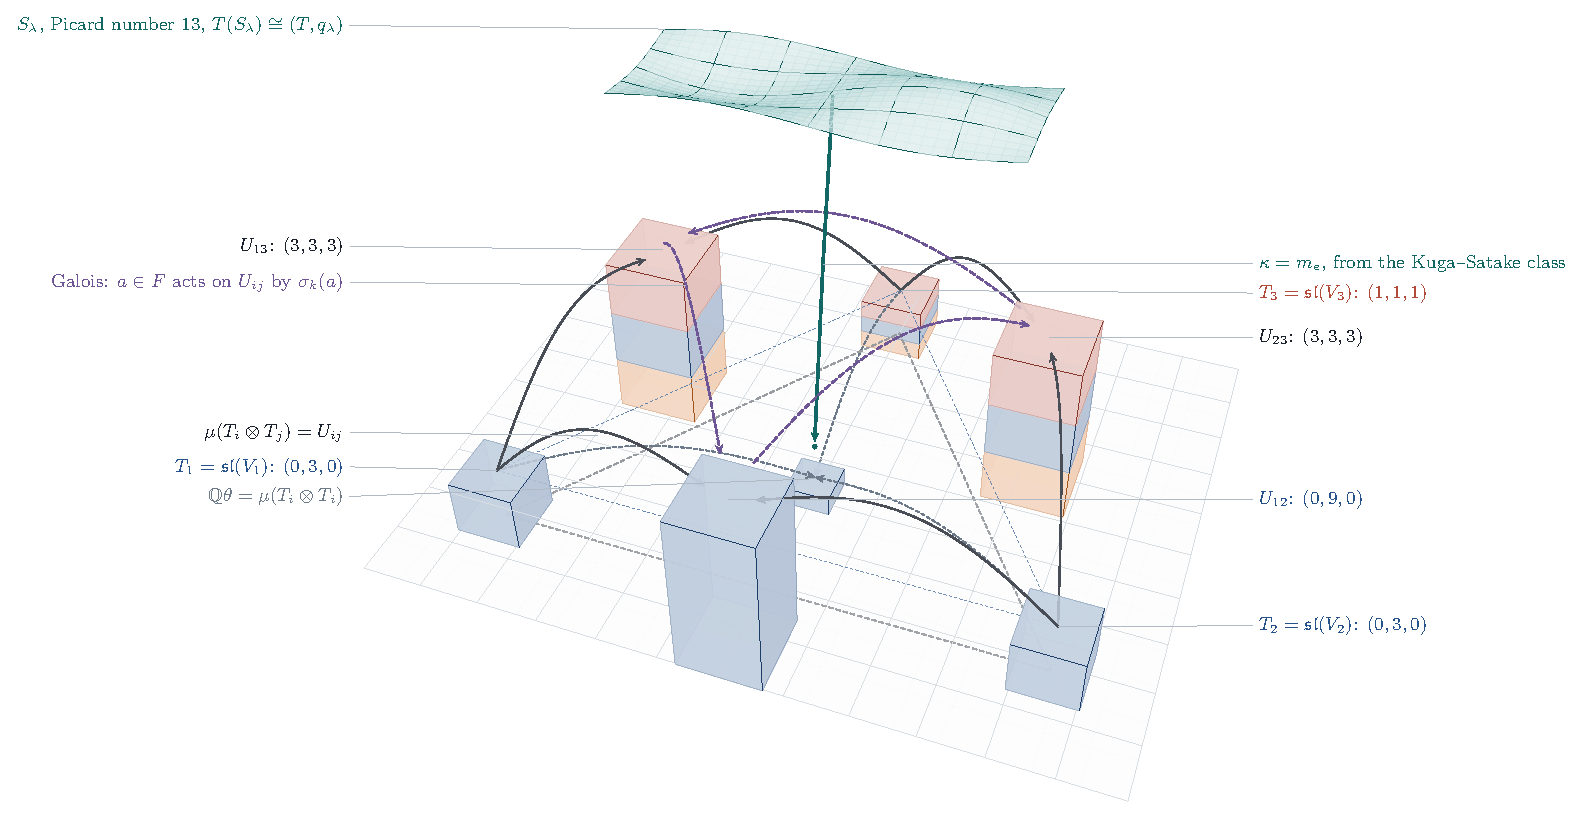
\includegraphics[width=\textwidth]{fig_mumford}
\caption{\Cref{prop:mumfordrm} and \Cref{lem:mumfordmu}, drawn over the
triangle of the three factors of the Hodge group; every height is a
dimension. At the corners stand the summands $T_{i}=\mathfrak{sl}(V_{i})$ of
$T=\operatorname{Lie}G$, banded by Hodge type after the Tate twist $T(-1)$: blue for
$(1,1)$, clay for $(2,0)$ and amber for $(0,2)$, so that only $T_{3}$ carries
the K3 type. On the edges stand the three summands $U_{ij}$ of the primitive
part of $H^{2}(X)$, of dimension nine, $U_{12}$ of pure type $(1,1)$ and the
other two in three bands of three; in the middle is the line of $\theta$. The
solid arcs are the product map $\mu$, which carries $T_{i}\otimes T_{j}$ onto
$U_{ij}$, and the dashed ones carry $T_{i}\otimes T_{i}$ to $\QQ\theta$. The
violet arcs are the Galois group permuting the $U_{ij}$ as it permutes the
embeddings of $F$, which is why the two exceptional classes may be taken to be
the trace-zero part of a cubic field. Above, the K3 surface $S_{\lambda}$ of
\Cref{thm:mumfordks}, whose Kuga--Satake class, if algebraic, comes down to
$T$ as the map $\kappa=m_{e}$.}
\label{fig:mumford}
\end{figure}

\begin{remark}[The Kuga--Satake class in the literature]
\label{rem:mumfordks}
\Cref{thm:mumfordks} takes the algebraicity of the Kuga--Satake class of
$S_{\lambda}$ as its input. The cases of the Kuga--Satake Hodge conjecture
proved in the literature are these. They include the projective K3 surfaces with
a Shioda--Inose structure, which relates the surface to an abelian surface;
by Morrison these are the surfaces of Picard number $19$ or $20$, those of
Picard number $18$ with $T(S)\cong U\oplus T'$ and those of Picard number
$17$ with $T(S)\cong U^{2}\oplus T'$
\cite[Theorem~6.3 and Corollary~6.4]{Mor84}, and for these the proof uses in
addition the Hodge conjecture for the powers of an abelian surface, whose
Hodge classes are generated by divisor classes (see \cite{MZ99}), and the
fact that the Kuga--Satake variety of an abelian surface is isogenous to a
power of it \cite{Mor85}. With Buskin's theorem that rational Hodge
isometries between K3 surfaces are algebraic \cite{Bus19}, this reaches the
surfaces of Picard number at least $19$, those of Picard number $18$ with
$T(S)_{\QQ}$ isotropic, and those of Picard number $17$ with $T(S)_{\QQ}$ of
Witt index two (\Cref{rem:mumfordpowersopen}). It does not reach every
surface of Picard number seventeen, as Morrison notes
\cite[Remark~7.2]{Mor84}: for
$T(S)=U\oplus\langle6\rangle\oplus\langle-2\rangle\oplus\langle-2\rangle$,
the transcendental lattice of the very general K3 surface of a family of
dimension three \cite[Corollary~2.10]{Mor84}, $T(S)_{\QQ}$ has Witt index one,
since $\langle6,-2,-2\rangle$ is anisotropic over $\QQ_{3}$: a primitive
solution of $3x^{2}=y^{2}+z^{2}$ in $\ZZ_{3}$ would have $3\mid y$ and
$3\mid z$, as $-1$ is not a square modulo $3$, and then $3\mid x$. The double planes branched along six lines, of Picard
number at least sixteen, are settled by Paranjape's cycle; see \cite{vG00}.
Floccari proves the conjecture for the K3 surfaces attached to projective
sixfolds of generalised Kummer type \cite{Flo24}, and then, for the K3
surfaces attached to all projective varieties of generalised Kummer type and
for every projective K3 surface $S$ with $T(S)_{\QQ}$ embedding isometrically
in $(U^{3}\oplus\langle-m\rangle)_{\QQ}$ for some $m>0$, both the conjecture
and the Hodge conjecture for all powers \cite[Theorems~1.2 and~5.11]{Flo25};
their transcendental lattices embed, after scaling in the first case, in a
rational quadratic space of rank seven and signature $(3,4)$, so their
transcendental rank is at most six. Ingalls, Logan and Patashnick prove the
conjecture, with the Hodge conjecture for the square, for a general K3
surface in $\PP^{4}$ with fifteen ordinary double points and for the K3
surfaces joined to it by chains of rational maps of finite degree
\cite[Theorems~1.5, 4.8 and~6.4]{ILP22}. Bolognesi and Laterveer prove it for
the triple covers of a quadric branched along a curve of genus four, which
form two families of dimension nine; these carry a non-symplectic
automorphism of order three, so their fields of Hodge endomorphisms are CM
fields \cite{BL24}. The surfaces $S_{\lambda}$, by contrast, have
transcendental rank nine and real multiplication by a cubic field, and none
of these cases contains them: a Shioda--Inose structure needs
$T(S)\cong T(A)$ for an abelian surface $A$, hence a transcendental rank of at
most five; the surfaces of Floccari, of Paranjape and of Ingalls, Logan and
Patashnick have transcendental rank at most six; and the field of Hodge
endomorphisms of $S_{\lambda}$ is totally real, not CM.

Schlickewei made the real multiplication algebraic on those double planes
that have it, necessarily by a field of degree at most two, from Paranjape's
cycle and van Geemen's description of their Kuga--Satake varieties
\cite{Sch10,vG08}, and Varesco showed that when the Kuga--Satake Hodge
conjecture holds for two hyperk\"ahler varieties, every Hodge similarity
between their transcendental lattices is algebraic up to the Lefschetz
isomorphism \cite{Var23}, which reaches a quadratic field through its square
root. More generally, if the Hodge endomorphisms of $T(S)$ form a totally
real field $E$, then $E$ acts by self-adjoint maps \cite{Zar83}, so $g\in E$
is a similarity, with multiplier $\mu$, exactly when $g^{2}=\mu\in\QQ$; the
Hodge similarities of $T(S)$ to itself, and with them all composites of Hodge
similarities between transcendental lattices of K3 surfaces that start and
end at $T(S)$, therefore span exactly the maximal multiquadratic subfield
$E_{\mathrm{mq}}$ of $E$, the compositum of its quadratic subfields. For a
cubic field $E_{\mathrm{mq}}=\QQ$: a cubic field contains no irrational
element with rational square, so no irrational element of it acts as a
similarity. In the proof of \Cref{thm:mumfordks} the element
$\kappa^{\dagger}\kappa=m_{4e^{2}/\lambda}$ plays the role that the
similarities play for quadratic fields, and the Clifford relations are what
make it irrational. Buskin's theorem \cite{Bus19} does not give the real
multiplication either. A Hodge isometry of $T(S_{\lambda})$ is a Hodge
endomorphism, hence some $m_{a}$ by \Cref{prop:mumfordrm}(iii), and it is an
isometry only when $a^{2}=1$. For $b\in F^{\times}$ Buskin's theorem does give
algebraic cycles between $S_{\lambda}$ and $S_{\lambda b^{-2}}$ that realise
$m_{b}$, but every composite of them that returns to $S_{\lambda}$ is again a
Hodge isometry of $T(S_{\lambda})$, so it multiplies by an element of square
one.

The surfaces $S_{\lambda}$ include those of Zhu, who computes the integral
structure that the fourfold induces on $T$ and studies the K3 surfaces of
Picard number thirteen that carry it \cite{Zhu18}; the form of that structure
is the corestriction of the reduced norm of $D^{0}$, which up to sign is
$\frac12q_{1}$. \Cref{thm:mumfordks} applies to them as it stands, because the
irrationality of $e^{2}/\lambda$ comes from the anticommuting blocks and not
from $\lambda$. The explicit families closest to these are those of van
Geemen and Sch\"utt, with
real multiplication by the cyclic cubic fields $\QQ(\zeta_{7}+\zeta_{7}^{-1})$
and $\QQ(\zeta_{9}+\zeta_{9}^{-1})$ and Picard numbers four and ten, on which
the real multiplication is induced by explicit algebraic cycles
\cite[Theorem~1.2 and Section~4.8]{vGS25}; their Picard numbers are not
thirteen, and the Kuga--Satake class, which \Cref{thm:mumfordks} needs and
algebraic real multiplication does not supply, is not treated there.

By \Cref{thm:mumfordks}, then, the first case of (F2) is implied by one
instance of the Kuga--Satake Hodge conjecture, for one K3 surface of Picard
number thirteen; by \Cref{prop:mumfordkslink} below that instance is
equivalent to the first case of (F2) at $X$ together with a link, and it is
not a reduction of it. The preprint \cite{OAI26c} announces that instance
for every K3 surface; its consequences are drawn in \Cref{sec:preprints}
(\Cref{cor:mumfordall}).
\end{remark}

\Cref{thm:mumfordks} trades the two exceptional classes for one Kuga--Satake
class. The next results make this exchange precise. If the
exceptional classes are algebraic, so is every Hodge class on every power of
$X$ (\Cref{thm:mumfordpowers}); if the Kuga--Satake class is algebraic, so is
every Hodge class on every product $S_{\lambda}^{a}\times X^{b}$
(\Cref{cor:mumfordksproducts}). The Kuga--Satake class is algebraic exactly
when the exceptional classes are and, in addition, some algebraic cycle links
$S_{\lambda}$ to a power of $X$ (\Cref{prop:mumfordkslink}), and no such link
can pass through an abelian variety of dimension at most five
(\Cref{prop:mumfordcarrier}). The theorem and the corollary are
implications, and \Cref{rem:mumfordpowersopen} collects the forms they give
to the first case of (F2).

\begin{proposition}[Where $T$ occurs]\label{prop:mumfordwhere}
In \Cref{setup:mumford}, write $\Hom_{\mathrm{Hdg}}$ for morphisms of rational
Hodge structures.
\begin{enumerate}[label=\textup{(\roman*)},nosep,leftmargin=2.6em]
\item $T$ is isomorphic to no subquotient of $H^{k}(X,\QQ)(j)$, for any $k$
  and $j$.
\item The $F$-vector space
  $\Hom_{\mathrm{Hdg}}\bigl(T,H^{2}(X\times X,\QQ)(1)\bigr)$ is
  one-dimensional, and the copy of $T$ in $H^{2}(X\times X,\QQ)(1)$ lies in
  $H^{1}(X)\otimes H^{1}(X)$. For $n$ odd and for $n\in\{0,16\}$ the Hodge
  structure $T$ is isomorphic to no subquotient of any
  $H^{n}(X\times X,\QQ)(j)$.
\item $\Hom_{\mathrm{Hdg}}(T,\End V)$ is a one-dimensional $F$-vector space,
  spanned by the inclusion. For $\lambda\in F$ totally positive, after an
  isogeny $\mathrm{KS}(S_{\lambda})\to X^{32}$ the Kuga--Satake embedding of
  $T(S_{\lambda})$ is a $32\times32$ matrix of maps $m_{e_{ab}}$ with
  $e_{ab}\in F$, and $\mathrm{KS}(S_{\lambda})$ is isogenous to $B^{4}$, where
  $B$ is isogenous to $X^{8}$ and $\End^{0}(B)=M_{8}(\QQ)$.
\end{enumerate}
\end{proposition}

\begin{proof}
After the twists all the Hodge structures involved have weight zero and lie in
the tensor category generated by $V$, whose Mumford--Tate group is
$G\cdot\mathbb{G}_{m}$ with $\mathbb{G}_{m}$ acting trivially in weight zero;
so their morphisms and subquotients are those of representations of $G$.
Over $\bar{\QQ}$, $T=T_{1}\oplus T_{2}\oplus T_{3}$ with $T_{i}\cong S^{2}V_{i}$,
and the Galois group permutes the three summands transitively. Hence $T$ is
irreducible, a representation of $G$ defined over $\QQ$ contains
$T_{1}$, $T_{2}$ and $T_{3}$ with one and the same multiplicity $m$, and its
space of $G$-maps from $T$, of $\QQ$-dimension $3m$, is a vector space over
$\End_{G}(T)=F$ (\Cref{prop:mumfordrm}(iii)) of dimension $m$.

For (i), write $V=V_{1}\otimes W$ with $W=V_{2}\otimes V_{3}$, on which
$\SL(V_{2})\times\SL(V_{3})$ acts through $\SO(W,q)$, $q$ the product of the
two symplectic forms. By the skew Cauchy formula
$\bigwedge^{k}V=\bigoplus_{\lambda}S_{\lambda}V_{1}\otimes S_{\lambda'}W$,
over the partitions $\lambda$ of $k$ with at most two rows and at most four
columns, and $S_{\lambda}V_{1}\cong S^{\lambda_{1}-\lambda_{2}}V_{1}$ as a
representation of $\SL(V_{1})$. So $T_{1}$ occurs in $\bigwedge^{k}V$ only
through $\lambda=(2,0)$, $(3,1)$ or $(4,2)$, and only if $S_{\lambda'}W$ has a
nonzero invariant under $\SL(V_{2})\times\SL(V_{3})$. As representations of
$\SL(W)$, $S_{(1,1)}W=\bigwedge^{2}W$, $S_{(2,2,1,1)}W\cong\bigwedge^{2}W$, and
$S_{(2,1,1)}W\cong\mathfrak{sl}(W)$, the kernel of the contraction
$\bigwedge^{3}W\otimes W\to\bigwedge^{4}W$ with $\bigwedge^{3}W\cong W^{*}$.
Restricted to $\SO(W,q)$, $\bigwedge^{2}W=\mathfrak{so}(W)=
\mathfrak{sl}(V_{2})\oplus\mathfrak{sl}(V_{3})$ and
$\mathfrak{sl}(W)=\mathfrak{so}(W)\oplus S^{2}V_{2}\otimes S^{2}V_{3}$, the
second summand being the trace-free part of $S^{2}W$; none of these has a
nonzero invariant. So $T_{1}$ occurs in no $\bigwedge^{k}V$, and by the same
argument with the factors exchanged neither do $T_{2}$ and $T_{3}$. As $G$ is
reductive, the subquotients of $\bigwedge^{k}V$ are its summands; that is (i).

For (ii),
$H^{n}(X\times X)=\bigoplus_{a+b=n}\bigwedge^{a}V\otimes\bigwedge^{b}V$. The
element of $G$ that is $-1$ on the first factor $\SL(V_{1})$ and $1$ on the
other two acts on $V$ by $-1$, hence on $H^{n}(X\times X)$ by $(-1)^{n}$, and
trivially on $T$; and $H^{0}$, $H^{16}$ are trivial representations. In
$H^{2}(X\times X)=\bigwedge^{2}V\oplus(V\otimes V)\oplus\bigwedge^{2}V$ the
summands $\bigwedge^{2}V$ contain no $T_{i}$ by (i), and
$V\otimes V=S^{2}V\oplus\bigwedge^{2}V$ with
\[
  S^{2}(V_{1}\otimes V_{2}\otimes V_{3})
  =S^{2}V_{1}\otimes S^{2}V_{2}\otimes S^{2}V_{3}
  \oplus\bigoplus_{i=1}^{3}S^{2}V_{i}\otimes
  \textstyle\bigwedge^{2}V_{j}\otimes\bigwedge^{2}V_{k},
\]
$\{i,j,k\}=\{1,2,3\}$, where $\bigwedge^{2}V_{j}$ is trivial. So each $T_{i}$
occurs exactly once in $H^{2}(X\times X)$, inside $V\otimes V$, and $m=1$.
For (iii), $\End V=S^{2}V\oplus
\bigwedge^{2}V$ contains each $T_{i}$ once, and the proof of
\Cref{thm:mumfordks}(ii) shows that the blocks of the Kuga--Satake embedding
are maps $m_{e_{ab}}$. Finally $\mathrm{KS}(S_{\lambda})$ is isogenous to
$X^{32}=(X^{8})^{4}$ by \Cref{thm:mumfordks}(i), and
$\End^{0}(X^{8})=M_{8}(\End^{0}X)=M_{8}(\QQ)$. This is the splitting
$\mathrm{KS}\sim B^{2^{d-1}}$, $d=[F:\QQ]$, which van Geemen proves for K3
surfaces with real multiplication \cite{vG08}; there $H^{1}(B,\QQ)$ is the
corestriction to $\QQ$ of the even Clifford algebra of $T$ over $F$, here
$D$, and over $\bar{\QQ}$ one has $\operatorname{Cor}_{F/\QQ}(D)=
\bigotimes_{k}D\otimes_{F,\sigma_{k}}\bar{\QQ}=\bigotimes_{k}\End(V_{k})=
\End(V)$, which is $V^{\oplus8}$ under left multiplication by $G$.
\end{proof}

\begin{theorem}[Every power of a Mumford fourfold]\label{thm:mumfordpowers}
In \Cref{setup:mumford}, suppose that the two exceptional classes of
\Cref{prop:mumfordproduct}(ii) are algebraic on $X\times X$. Then every Hodge
class on $X^{n}$ is algebraic, for every $n\ge1$.
\end{theorem}

\begin{proof}
Over $\bar{\QQ}$ keep $V=V_{1}\otimes V_{2}\otimes V_{3}$ and
$\psi=\epsilon_{1}\otimes\epsilon_{2}\otimes\epsilon_{3}$, as in the proof of
\Cref{lem:mumfordmu}. For $m\ge1$ regard $V^{\otimes m}=H^{1}(X)^{\otimes m}$
as the K\"unneth component of $H^{m}(X^{m},\QQ)$ of multidegree
$(1,\dots,1)$, whose projector is algebraic \cite[\S2]{Kle68}. Call an
endomorphism of $V^{\otimes m}$ algebraic if it is the action on
$V^{\otimes m}$ of an algebraic cycle on $X^{m}\times X^{m}$ that preserves
$V^{\otimes m}$. Composing with the K\"unneth projector, the algebraic
endomorphisms form a $\QQ$-algebra, and they carry algebraic classes in
$V^{\otimes m}$ to algebraic classes.

\emph{Step 1: reduction to multilinear invariants.} Let $n\ge1$ and $p\ge0$.
The map $V^{\otimes2p}\otimes(\QQ^{n})^{\otimes2p}\to
\bigwedge^{2p}(V\otimes\QQ^{n})=H^{2p}(X^{n},\QQ)$ sending
$(v_{1}\otimes\dots\otimes v_{2p})\otimes(a_{1}\otimes\dots\otimes a_{2p})$ to
$(v_{1}\otimes a_{1})\wedge\dots\wedge(v_{2p}\otimes a_{2p})$ is surjective
and $G$-equivariant for the trivial action on $\QQ^{n}$, so it is surjective
on $G$-invariants, $G$ being reductive. For $a_{1},\dots,a_{2p}\in\ZZ^{n}$
the image of $t\otimes(a_{1}\otimes\dots\otimes a_{2p})$ is $f^{*}t$, where
$f\colon X^{n}\to X^{2p}$ is the homomorphism with rows $a_{1},\dots,a_{2p}$,
and such tensors span $(\QQ^{n})^{\otimes2p}$. So $\Hdg^{p}(X^{n})$ is
spanned by the classes $f^{*}t$ with $f$ a homomorphism and
$t\in(V^{\otimes2p})^{G}$, and it suffices to show that every element of
$(V^{\otimes2p})^{G}$ is algebraic.

\emph{Step 2: degree four.} The space $(V^{\otimes4})^{G}$ has dimension
eight, the product of the dimensions of the three spaces of
$\SL_{2}$-invariants in $V_{k}^{\otimes4}$. Let $\cP_{0}\subset
(V^{\otimes4})^{G}$ be the span of the multilinear components of the classes
$f^{*}\xi$, for $\xi\in\Hdg^{2}(X\times X)$ and $f\colon X^{4}\to X^{2}$ a
homomorphism, and of the products of two divisor classes of $X^{4}$. By
\Cref{prop:mumfordproduct}(ii) $\Hdg^{2}(X\times X)$ is spanned by the six
products of divisor classes and the two exceptional classes, so under the
hypothesis every element of $\cP_{0}$ is algebraic. For
$t\in V^{\otimes4}$, read as a correspondence from the first two factors of
$X^{4}$ to the last two, let $\hat{t}$ be the endomorphism
$v\mapsto t_{*}\bigl((\theta^{3}\times\theta^{3})\cup v\bigr)$ of
$V\otimes V$. The pairing $(v,w)\mapsto\int_{X}v\cup w\cup\theta^{3}$ on $V$
is nondegenerate by hard Lefschetz and $G$-invariant, so $t\mapsto\hat{t}$
is an isomorphism $(V^{\otimes4})^{G}\to\End_{G}(V\otimes V)$, and $\hat{t}$
is algebraic when $t$ is. We show that the $\hat{t}$ and the composites
$\hat{u}\hat{t}$, for $t,u\in\cP_{0}$, span $\End_{G}(V\otimes V)$. Over
$\bar{\QQ}$, $\End_{G}(V\otimes V)=\bigotimes_{k}\End_{\SL_{2}}(V_{k}\otimes
V_{k})$ is the algebra of functions on the eight sign patterns
$\varepsilon\in\{\pm1\}^{3}$, where $\varepsilon_{k}$ is the eigenvalue of the
exchange $s_{k}$ of the two copies of $V_{k}$; the patterns with
$\varepsilon_{1}\varepsilon_{2}\varepsilon_{3}=-1$, the odd ones, make up
$\bigwedge^{2}V$.

(a) Let $f=(x_{1}+x_{2},x_{3}+x_{4})\colon X^{4}\to X^{2}$. The multilinear
component of $f^{*}\xi$ depends only on the K\"unneth component of $\xi$ in
$H^{2}(X)\otimes H^{2}(X)$, and it is that component read as a tensor
$t\in\bigwedge^{2}V\otimes\bigwedge^{2}V$, so $\hat{t}$ vanishes on $S^{2}V$
and takes values in $\bigwedge^{2}V$. These components fill
$(H^{2}\otimes H^{2})^{G}=\End_{G}(H^{2})$, of dimension $4$ by
\Cref{prop:mumfordrm}(ii); so the $\hat{t}$ span the functions supported on
the four odd patterns.

(b) The map $g=(x_{1}+x_{3},x_{2}+x_{4})$ is $f$ composed with the exchange
of the factors $2$ and $3$ of $X^{4}$, which permutes the factors of
$V^{\otimes4}$ up to sign. On $V_{k}^{\otimes4}$ the $\SL_{2}$-invariants are
spanned by $\epsilon_{13}\epsilon_{24}$, $\epsilon_{14}\epsilon_{23}$ and
$\epsilon_{12}\epsilon_{34}=\epsilon_{13}\epsilon_{24}-\epsilon_{14}
\epsilon_{23}$, where $\epsilon_{ab}$ is $\epsilon_{k}$ on the factors $a$ and
$b$; up to a common sign their hats are $1$, $s_{k}$ and $1-s_{k}$. The
exchange of the factors $2$ and $3$ swaps the first and the third and changes
the sign of the second, so on functions of $\varepsilon_{k}$ it carries
$\frac12(1-s_{k})$ to $\frac12$ and $\frac12(1+s_{k})$ to $\frac12-s_{k}$.
Applied to the indicator of the odd pattern $(1,1,-1)$ it gives
$\frac12(\frac12-s_{1})(\frac12-s_{2})$. The identity is $\hat{t}$ for the
multilinear component of a product of two divisor classes, the pull-backs of
the class $\psi$ on $X\times X$ along the projections of $X^{4}$ to the
factors $(1,3)$ and $(2,4)$, so $h=(1-2s_{1})(1-2s_{2})-1$ lies in the span of the
$\hat{t}$, $t\in\cP_{0}\otimes\bar{\QQ}$. As $(\varepsilon_{1},\varepsilon_{2})$
runs through $(1,1)$, $(1,-1)$, $(-1,1)$, $(-1,-1)$, $h$ takes the values
$0,-4,-4,8$, so $h(h+4)/96$ is the indicator of
$\varepsilon_{1}=\varepsilon_{2}=-1$; subtracting the indicator of
$(-1,-1,-1)$, from (a), leaves that of $(-1,-1,1)$. The same argument with the
factors $V_{k}$ permuted gives the other two even patterns with two minus
signs, and the indicator of $(1,1,1)$ is $1$ minus the other seven.

So the $\hat{t}$ and $\hat{u}\hat{t}$ span $\End_{G}(V\otimes V)\otimes
\bar{\QQ}$. Since composition is bilinear and $\cP_{0}\otimes
\bar{\QQ}$ is spanned by the same pull-backs and products of a basis of
Hodge classes, the $\QQ$-algebra of algebraic $G$-endomorphisms of
$V\otimes V$ has dimension $8$: every $G$-endomorphism of $V\otimes V$ is
algebraic.

\emph{Step 3: the partial swaps.} Over $\bar{\QQ}$,
$\End_{G}(V\otimes V)=\bigotimes_{k}\End_{\SL_{2}}(V_{k}\otimes V_{k})$, and
$\End_{\SL_{2}}(V_{k}\otimes V_{k})$ is spanned by $1$ and the exchange $s_{k}$
of the two copies of $V_{k}$. In a basis of $V_{k}$ the matrix units
$E_{ab}$ and $E_{ba}$ are dual for the trace form of $\mathfrak{gl}(V_{k})$,
and $\sum_{a,b}E_{ab}\otimes E_{ba}=s_{k}$; removing the centre, spanned by the
identity $1$ with $\operatorname{tr}(1\cdot1)=2$, gives
$s_{k}=\mathrm{Cas}_{k}+\frac12$, with $\mathrm{Cas}_{k}=\sum_{c}x_{c}\otimes
x^{c}$ for dual bases $(x_{c})$, $(x^{c})$ of $\mathfrak{sl}(V_{k})$ under the
trace form. So the $s_{k}$ come from the three summands $T_{k}$ of $T$. The Galois group permutes the $s_{k}$ as it
permutes the embeddings $\sigma_{k}$, so for $a\in F$ the endomorphism
$r_{a}=\sum_{k}\sigma_{k}(a)s_{k}$ is rational, hence algebraic by Step 2. For
$m\ge2$ and $1\le i<m$ let $r_{a}^{(i)}$ and $s_{k}^{(i)}$ act as $r_{a}$ and
$s_{k}$ on the factors $i$ and $i+1$ of $V^{\otimes m}$ and as the identity on
the others; $r_{a}^{(i)}$ is algebraic, being induced by the product of a cycle
inducing $r_{a}$ with the diagonals of the other factors. By Schur--Weyl
duality $\End_{\SL_{2}}(V_{k}^{\otimes m})$ is the image of
$\bar{\QQ}[S_{m}]$, generated by the adjacent transpositions, and the
commutant of $\SL_{2}^{3}$ in $\bigotimes_{k}V_{k}^{\otimes m}$ is the tensor
product of the three commutants; so $\End_{G}(V^{\otimes m})\otimes\bar{\QQ}$
is generated by the $s_{k}^{(i)}$. For a basis $a_{1},a_{2},a_{3}$ of $F$ the
matrix $(\sigma_{k}(a_{j}))$ is invertible, the square of its determinant being
the discriminant of $F$, so each $s_{k}^{(i)}$ is a $\bar{\QQ}$-linear
combination of the $r_{a_{j}}^{(i)}$. The $\QQ$-algebra generated by the
$r_{a}^{(i)}$ therefore lies in $\End_{G}(V^{\otimes m})$ and spans it over
$\bar{\QQ}$, so it is $\End_{G}(V^{\otimes m})$: every $G$-endomorphism of
$V^{\otimes m}$ is algebraic. Its dimension is the cube of
$\dim\End_{\SL_{2}}(V_{k}^{\otimes m})$, the sum of the squares of the
multiplicities in $V_{k}^{\otimes m}$: $8=2^{3}$ for $m=2$ and $125=5^{3}$ for
$m=3$, where $V_{k}^{\otimes3}=S^{3}V_{k}\oplus V_{k}^{\oplus2}$.

\emph{Step 4: all multilinear invariants.} By the first fundamental theorem
for $\SL_{2}$ the invariants in $V_{k}^{\otimes2m}$ are spanned by the images
of $\epsilon_{k}^{\otimes m}$ under the permutations of the $2m$ factors. So
$(V^{\otimes2m})^{G}\otimes\bar{\QQ}$ is spanned by the images of
$\psi^{\otimes m}=\bigotimes_{k}\epsilon_{k}^{\otimes m}$ under the operators
that permute the factors of the three $V_{k}^{\otimes2m}$ separately, which
lie in $\End_{G}(V^{\otimes2m})\otimes\bar{\QQ}$, and the map
$\End_{G}(V^{\otimes2m})\to(V^{\otimes2m})^{G}$, $e\mapsto e(\psi^{\otimes m})$,
is surjective. The class $\psi$ in $V\otimes V$ is that of the divisor
$m^{*}\theta-p_{1}^{*}\theta-p_{2}^{*}\theta$ on $X\times X$ (proof of
\Cref{thm:mumfordks}(ii)), up to a nonzero factor, and $\psi^{\otimes m}$ is,
up to sign, the product of its pull-backs along the projections of $X^{2m}$
to the pairs of factors $(2j-1,2j)$; so it is algebraic, and by Step 3 so is
every element of $(V^{\otimes2m})^{G}$. Step 1 concludes.
\end{proof}

\begin{remark}[Why a composite is needed]\label{rem:mumforddet}
Step 2 cannot be carried out with pull-backs and products alone. The skew
Cauchy decomposition $\bigwedge^{4}(V\otimes\QQ^{4})=\bigoplus_{\lambda}
S_{\lambda}V\otimes S_{\lambda'}\QQ^{4}$, over the partitions $\lambda$ of $4$
with conjugates $\lambda'$, is functorial in $\QQ^{4}$, and its summand
$S^{4}V\otimes\bigwedge^{4}\QQ^{4}$ contains exactly one line of Hodge classes
of $X^{4}$: $S_{4}$ acts on the two-dimensional space of $\SL_{2}$-invariants
in $V_{k}^{\otimes4}$ through its two-dimensional irreducible representation
$\sigma$, and the trivial representation occurs once in $\sigma^{\otimes3}$.
That line is spanned by a class $\mathrm{Det}\in(V^{\otimes4})^{G}$ on which
the permutations of the factors of $X^{4}$ act by the sign, and whose
restriction to the diagonal, on the split model
$V=\bar{\QQ}^{2}\otimes\bar{\QQ}^{2}\otimes\bar{\QQ}^{2}$, is an invariant
quartic form of $\SL_{2}^{3}$, hence a nonzero multiple of Cayley's
hyperdeterminant. Pull-backs along homomorphisms
$X^{4}\to X^{2}$ have no component in that summand, because
$\bigwedge^{4}\QQ^{2}=0$, and products of divisor classes have none, because
they are invariant under $\Sp(V,\psi)$ and $S^{4}V$ has no
$\Sp(V,\psi)$-invariant. In the notation of Step 2 the hats of the elements
of $\cP_{0}$ therefore satisfy one linear condition, which is
$v_{(1,-1,-1)}+v_{(-1,1,-1)}+v_{(-1,-1,1)}=3v_{(1,1,1)}$ for the values $v$ on
the even patterns, since the functions found in (a) and (b), those supported
on the odd patterns, the constant, $h$ and its two images under the
permutations of the factors $V_{k}$, satisfy it and
span a space of dimension $7$. So $\cP_{0}$ has dimension $7$ and is the space
of Hodge classes of $X^{4}$ in the multilinear parts of the other summands,
and $\mathrm{Det}$ is reached only through a composite of correspondences,
which involves a push-forward. The composite $h^{2}$ of Step 2 is one: the
indicator of $(-1,-1,1)$ violates the condition. This is where
\Cref{thm:mumfordpowers} differs from \Cref{prop:powers}, in which the first
fundamental theorem for $\SL(W)$ lets pull-backs and products suffice. We have
not found \Cref{thm:mumfordpowers} in the literature; it is an implication
between two cases of the Hodge conjecture.
\end{remark}

At the CM points of a Mumford family the conclusion holds without any
hypothesis.

\begin{proposition}[Powers at a CM point]\label{prop:mumfordcmpowers}
Let $W\to C$ be a family as in \Cref{cor:mumfordlefschetz} and $c\in C$ a CM
point. Then the Hodge conjecture holds for $X_{c}^{n}$ for every $n\ge1$.
\end{proposition}

\begin{proof}
The proof of \Cref{thm:mumfordcm} shows that for every $n\ge1$ the ring
$\Hdg^{*}(X_{c}^{n})$ is generated by pull-backs of Hodge classes of the
fourfold $X_{c}$ along homomorphisms $X_{c}^{n}\to X_{c}$, and these are
algebraic \cite{Mar25a}.
\end{proof}

The statement is also contained in the theorem of \cite{Li26} on the
powers of CM fourfolds.

\begin{corollary}[Powers and fibre powers of a Mumford family]
\label{cor:mumfordpowersequiv}
Let $W\to C$ be as in \Cref{cor:mumfordlefschetz} and, for $n\ge1$, let
$W^{(n)}=W\times_{C}\dots\times_{C}W$, with $n$ factors. The conditions of
\Cref{cor:mumfordequiv} are equivalent to each of the following.
\begin{enumerate}[label=\textup{(\alph*)},start=5,leftmargin=2.6em,itemsep=2pt]
\item The Hodge conjecture holds for $X_{t}^{n}$ for every $t\in C$ and
  every $n\ge1$.
\item $B(W^{(n)})$ holds for $L_{W^{(n)}}$ for every $n\ge1$.
\end{enumerate}
\end{corollary}

\begin{proof}
(b) implies (e): by \Cref{cor:mumfordequiv}, (b) gives (c), so the
exceptional classes of $X_{t}\times X_{t}$ are algebraic for every $t$. At a
point $t$ that is not a CM point the Hodge group of $X_{t}$ is $G$, as shown
in the proof of \Cref{cor:mumfordequiv}, and \Cref{thm:mumfordpowers}
applies; at a CM point \Cref{prop:mumfordcmpowers} does. (e) implies (f):
$W^{(n)}$ is an abelian scheme over $C$ with projective total space, and, as
in the proof of \Cref{cor:lefschetzsmall}, its monodromy invariant classes are
Hodge classes on every fibre; by (e) they are algebraic on every fibre, hence
restrictions of algebraic classes on $W^{(n)}$ by \Cref{lem:spreading}, and
\Cref{thm:lefschetzfamily} gives $B(W^{(n)})$. (f) implies (a): take $n=2$.
\end{proof}

\begin{corollary}[Products with the K3 surface]\label{cor:mumfordksproducts}
In \Cref{setup:mumford}, let $\lambda\in F$ be totally positive and
$S=S_{\lambda}$ as in \Cref{thm:mumfordks}. If the Kuga--Satake class of $S$
is algebraic, then the Hodge conjecture holds for $S^{a}\times X^{b}$ for all
$a,b\ge0$.
\end{corollary}

\begin{proof}
By \Cref{thm:mumfordks}(ii) the exceptional classes are algebraic, so by
\Cref{thm:mumfordpowers} the Hodge conjecture holds for every power of $X$.
In the proof of \Cref{thm:mumfordks}(ii) a block $\kappa=m_{e}$, $e\ne0$, of
the Kuga--Satake embedding is induced by a cycle on $S\times X\times X$; it
is a map from $T(S)$ to $\End V$, which up to a twist is a K\"unneth
component of $H^{*}(X\times X,\QQ)$. Its adjoint $\kappa^{\dagger}$ is
algebraic, $\kappa^{\dagger}\kappa=m_{4e^{2}/\lambda}$, and every $m_{a}$,
$a\in F$, is induced by a cycle on $S\times S$. So
$L=m_{\lambda/(4e^{2})}\kappa^{\dagger}$ is algebraic and $L\kappa$ is the
identity of $T(S)$. The decomposition
$H^{*}(S,\QQ)=\QQ\oplus\NS(S)_{\QQ}\oplus T(S)\oplus H^{4}(S,\QQ)$ has
algebraic projectors, as in that proof, so $H^{*}(S^{a}\times X^{b},\QQ)$ is
the sum of the summands $N\otimes T(S)^{\otimes r}\otimes H^{*}(X^{b},\QQ)$,
$N$ a tensor product of $a-r$ of the three other pieces, each cut out by an
algebraic projector. Each such $N$ is spanned by products of algebraic classes
and is of Tate type, so a Hodge class in the summand is a sum of products
$p^{*}\eta\cup q^{*}\xi$ with $\eta$ algebraic on $S^{a-r}$ and $\xi$ a Hodge
class in $T(S)^{\otimes r}\otimes H^{*}(X^{b},\QQ)\subset H^{*}(S^{r}\times
X^{b},\QQ)$. For such $\xi$ the class $(\kappa^{\otimes r}\otimes1)\xi$ is a
Hodge class on $X^{2r+b}$, hence algebraic, and
$\xi=(L^{\otimes r}\otimes1)(\kappa^{\otimes r}\otimes1)\xi$ is algebraic.
\end{proof}

\Cref{cor:mumfordksproducts} strengthens \Cref{thm:mumfordks}(ii), which gives
$X\times X$ only. Varesco proves an implication of the same kind, from the
algebraicity of the Kuga--Satake correspondence to the Hodge conjecture for
all powers, for families of K3 surfaces of generic Picard number sixteen
\cite{Var22}. The converse question, what the Kuga--Satake class asks for
beyond the target, has a precise answer.

\begin{proposition}[What the Kuga--Satake route asks]\label{prop:mumfordkslink}
In the situation of \Cref{cor:mumfordksproducts}, the Kuga--Satake class of
$S$ is algebraic if and only if
\begin{enumerate}[label=\textup{(\roman*)},nosep,leftmargin=2.6em]
\item the two exceptional classes of $X\times X$ are algebraic, and
\item \textup{(}a link\textup{)} for some $n\ge1$ there is an algebraic cycle
  $Z$ on $S\times X^{n}$ whose action $Z_{*}$ is nonzero on $T(S)$.
\end{enumerate}
\end{proposition}

\begin{proof}
If the Kuga--Satake class is algebraic, (i) is \Cref{thm:mumfordks}(ii), and a
nonzero block of the embedding, induced by a cycle on $S\times X\times X$, is
a link with $n=2$. Conversely assume (i) and (ii). By
\Cref{thm:mumfordpowers} the Hodge conjecture holds for every power of $X$.
Since $T(S)\cong T(-1)$ is irreducible (proof of \Cref{prop:mumfordwhere}),
$Z_{*}$ maps $T(S)$ isomorphically onto a sub-Hodge structure of some
$H^{2k}(X^{n},\QQ)(k-1)$, which is a direct summand, polarisable Hodge
structures being semisimple. Projecting onto it and composing with an
isomorphism onto the copy of $T(-1)$ in $H^{2}(X\times X,\QQ)$
(\Cref{prop:mumfordwhere}(ii)) gives a morphism of Hodge structures
$H^{2k}(X^{n},\QQ)(k-1)\to H^{2}(X\times X,\QQ)$, that is a Hodge class on
$X^{n+2}$, which is algebraic. Its composite with $Z_{*}$ is an algebraic
nonzero morphism $T(S)\to T(-1)\subset H^{2}(X\times X,\QQ)$, which is some
$m_{e}$, $e\ne0$, by \Cref{prop:mumfordrm}(iii). The endomorphisms of
$H^{2}(X\times X,\QQ)$ that act by $m_{a}$ on this copy of $T(-1)$ and by zero
on a Hodge complement are Hodge classes on $X^{4}$, hence algebraic, so every
$m_{a}\colon T(S)\to H^{1}(X)\otimes H^{1}(X)$, $a\in F$, is algebraic, and so is
its composite with cup product with $\theta^{3}$ on one factor, which carries
$H^{1}(X)\otimes H^{1}(X)$ onto the K\"unneth component of $H^{8}(X\times X,\QQ)$
that represents $\End V$. By \Cref{prop:mumfordwhere}(iii), after an isogeny
$\mathrm{KS}(S)\to X^{32}$ the Kuga--Satake embedding is a matrix of such
maps, and the Kuga--Satake class is recovered from its blocks through the
graphs of the isogeny and of the inclusions and projections of the factors of
$X^{32}$; so it is algebraic.
\end{proof}

So the Kuga--Satake route is at least as strong as the first case of (F2) and
is not a reduction of it: at the point $X$ it asks for (i), which is the first
case of (F2) there, and in addition for a link. The Hodge conjecture
implies both (i) and (ii). The route helps only if the
Kuga--Satake class of $S_{\lambda}$ can be made algebraic by arguments proper
to K3 surfaces. A link has to be a correspondence of a new kind: $T$ occurs
in no $H^{k}(X)$ (\Cref{prop:mumfordwhere}(i)), and the next proposition
shows that it occurs in the cohomology of no abelian variety of dimension
below six.

\begin{proposition}[No small abelian carrier of $T$]\label{prop:mumfordcarrier}
In \Cref{setup:mumford}, let $Y$ be an abelian variety such that $T(-1)$ is
isomorphic to a subquotient of $H^{k}(Y,\QQ)(j)$ for some $k$ and $j$. Then
$\dim Y\ge6$. Consequently, if $\dim Y\le5$ and $S=S_{\lambda}$ is as in
\Cref{thm:mumfordks}, every Hodge class on $S\times Y$, algebraic or not, acts
by zero on $T(S)$, and no link as in \Cref{prop:mumfordkslink}(ii) is a
composite $Z_{2}\circ Z_{1}$ of algebraic cycles on $S\times Y$ and on
$Y\times X^{n}$.
\end{proposition}

\begin{proof}
Write $W=T(-1)$. As $W$ is a subquotient of a tensor construction on
$H^{1}(Y)$, $\MT(Y)$ maps onto $\MT(W)$, whose derived group is the adjoint
group $G^{\mathrm{ad}}$ of $G$, acting on $W$ through the adjoint
representation. So the derived group of $\Hg(Y)$, an almost direct product of
$\QQ$-simple groups, maps onto $G^{\mathrm{ad}}$. The image of each factor is
a normal subgroup of the $\QQ$-simple group $G^{\mathrm{ad}}$, the images
commute, and $G^{\mathrm{ad}}$ is not commutative, so exactly one factor $M$
maps onto $G^{\mathrm{ad}}$, with finite kernel. Over $\bar{\QQ}$, $M$ is
isogenous to $\SL_{2}^{3}$, with factors indexed by the embeddings
$\sigma_{1},\sigma_{2},\sigma_{3}$ and permuted transitively by the Galois
group, and the irreducible constituents of $H^{1}(Y,\bar{\QQ})$ under $M$ are
products $R_{1}\otimes R_{2}\otimes R_{3}$ of irreducible representations of
the three factors.

Let $\mu_{Y}$ be the Hodge cocharacter of $Y$, with the two weights $0$ and
$1$ on $H^{1}(Y)$, and write $\mu_{Y}=\mu'\mu''$ with fractional cocharacters
$\mu'$ of $M$ and $\mu''$ commuting with $M$. The image of $\mu''$ in
$\MT(W)$ commutes with $G^{\mathrm{ad}}$, so it is central, and the image of
$\mu'$ in $G^{\mathrm{ad}}$ is the component there of the Hodge cocharacter of
$W$, which by \Cref{prop:mumfordrm}(iii) is trivial on the factors at
$\sigma_{1}$ and $\sigma_{2}$ and has weights $-1,0,1$ on $T_{3}$. So $\mu'$
is trivial on the first two factors of $M$ and has weights $\pm\frac12$ on
the standard representation of the third. On
$R_{1}\otimes R_{2}\otimes R_{3}$, tensored with an eigenvector of $\mu''$
in its multiplicity space, the weights of $\mu_{Y}$ therefore fill an
interval of length $\dim R_{3}-1$, so
$\dim R_{3}\le2$. The constituents form a Galois-stable multiset and the
Galois group carries the third factor to each of the others, so every
constituent is $V_{I}=\bigotimes_{i\in I}V_{i}$ for a subset
$I\subseteq\{1,2,3\}$, with a multiplicity $m_{I}$ that depends only on $|I|$,
and $m_{I}\ne0$ for some nonempty $I$, since $M$ acts nontrivially.

If $m_{I}\ne0$ for some $I$ with $|I|=2$, then $\dim H^{1}(Y)\ge3\cdot4=12$.
If $m_{\{1\}}\ne0$, let $U=V_{1}\otimes N$, $\dim N=m_{\{1\}}$, be the
$V_{1}$-isotypic summand of $H^{1}(Y,\CC)$. The embedding $\sigma_{1}$ is
real, so complex conjugation preserves the first factor of $M$ and $U$ is
defined over $\RR$. The connected group $\MT(Y)$ acts on $M$ preserving each
factor, and $\SL_{2}$ has a single irreducible representation of dimension
two, so $U$ is stable under $\MT(Y)(\RR)$ and is a real sub-Hodge structure
of $H^{1}(Y,\RR)$, and $U^{1,0}$ and $U^{0,1}$ are complex conjugate and
both nonzero. Since $\mu'$ acts trivially on $U$, $\mu_{Y}$ acts on
$V_{1}\otimes N$ through $N$, so $N$ carries both weights, $m_{\{1\}}\ge2$, and
$\dim H^{1}(Y)\ge3\cdot2\cdot2=12$. Otherwise $H^{1}(Y,\bar{\QQ})$ is
$V^{\oplus m}$, $m\ge1$, plus a trivial representation of $M$. If $m=1$,
every $H^{k}(Y)$ is, as a representation of $M$, a sum of copies of the
$\bigwedge^{a}V$, none of which contains an $S^{2}V_{i}$
(\Cref{prop:mumfordwhere}(i)), while $W$ contains all three; so $m\ge2$ and
$\dim H^{1}(Y)\ge16$. In every case $\dim Y=\frac12\dim H^{1}(Y)\ge6$.

For the rest, a Hodge class on $S\times Y$ acting nontrivially on the
irreducible $T(S)\cong W$ carries it isomorphically onto a sub-Hodge structure
of some $H^{k}(Y,\QQ)(j)$, and if $Z_{2}\circ Z_{1}$ acts nontrivially on
$T(S)$, so does $Z_{1}$.
\end{proof}

Among the powers of $X$ the smallest carrier of $T$ is $X\times X$, of
dimension eight, where $T(-1)$ sits in $H^{2}$
(\Cref{prop:mumfordwhere}(ii)). Whatever is known about abelian varieties of
dimension at most five, in particular Markman's theorem in dimension four
\cite{Mar25a}, no link passes through one.

\begin{remark}[The bound six as a statement about Hodge structures]
\label{rem:mumfordunitary}
The bound of \Cref{prop:mumfordcarrier} is, as far as we know, the best that
Hodge theory gives. Let $K\subset D$ be a CM quadratic extension of $F$,
$\chi_{i}$ the character of the $i$-th factor of the torus
$\Res_{F/\QQ}K^{1}$ over $\bar{\QQ}$, and
$H=\bigoplus_{i}(V_{i}\chi_{i}\oplus V_{i}\chi_{i}^{-1})$, of dimension twelve,
with types $(1,0)$ on $V_{i}\chi_{i}$ and $(0,1)$ on $V_{i}\chi_{i}^{-1}$ for
$i=1,2$, and with the Hodge cocharacter of $V_{3}$ on the two summands with
$i=3$: the signature $(2,0)$, $(2,0)$, $(1,1)$. The characters
$\chi_{i}^{\pm1}\chi_{j}^{\pm1}$ with $i\ne j$ and $\chi_{i}^{\pm2}$ are
nontrivial, so the part of $\bigwedge^{2}H$ on which the torus acts trivially
is $\bigoplus_{i}V_{i}\chi_{i}\otimes V_{i}\chi_{i}^{-1}=\bigoplus_{i}
(S^{2}V_{i}\oplus\bigwedge^{2}V_{i})$, that is, $T_{1}\oplus T_{2}\oplus T_{3}$
plus three trivial summands. For $i=1,2$ the summand $T_{i}$ is of type
$(1,1)$, and $S^{2}V_{3}$ has one dimension in each of the types $(2,0)$,
$(1,1)$, $(0,2)$, so this copy of $T$ has Hodge numbers $(1,7,1)$, those of
$T(S_{\lambda})$. We recall
without proof that these are the Hodge structures on $H^{1}(Z,\QQ)\cong D$ of
the abelian sixfolds $Z$ with multiplication by $K$ over the Shimura curves of
PEL type attached to $K$ and $D$, which go back to Shimura, and that at a
suitable member the copy of $T$ is isomorphic to $T(S_{\lambda})$, the Hodge
structure on it depending only on the image of the Hodge cocharacter in
$G^{\mathrm{ad}}$. Nothing in the paper uses this, and it would not give a
link: that would still need an algebraic cycle on $S_{\lambda}\times Z$ acting
nontrivially on $T(S_{\lambda})$.
\end{remark}

\begin{remark}[The K3 surfaces at the CM points]\label{rem:mumfordkscm}
Apply the construction of \Cref{thm:mumfordks}(i) at a CM point $c$ of a
family as in \Cref{cor:mumfordlefschetz}, with the Hodge structure that
$X_{c}$ induces on $T$, and call the surface $S_{c}$. By the proof of
\Cref{thm:mumfordcm} the Hodge group of $X_{c}$ is $\Res_{F/\QQ}L^{1}$ for a
quadratic extension $L$ of $F$ contained in $D$; $L$ is a CM field, since the
torus is compact at $\sigma_{1}$ and $\sigma_{2}$, where $D$ is definite, and
at $\sigma_{3}$, where it contains the nontrivial image of the circle of the
Hodge structure. The torus acts on $T=D^{0}$ by conjugation, with invariants
$D^{0}\cap L$, the three-dimensional space $L^{0}$ of elements of $L$ of
reduced trace zero. So $\NS(S_{c})_{\QQ}=T^{\perp}\oplus L^{0}$ has rank
sixteen. Write $D=L\oplus Lj$ with $jx=\bar{x}j$ for $x\in L$. Then $Lj$ is
the $q_{\lambda}$-orthogonal complement of $L^{0}$ in $D^{0}$, because
$\operatorname{trd}(yj)=0$ for $y\in L$, so $T(S_{c})_{\QQ}=Lj$ has rank six;
$t\in L^{1}$ acts on it by multiplication by $t^{2}$, so left multiplication
by $L$ consists of Hodge endomorphisms and $T(S_{c})$ has complex
multiplication by the sextic CM field $L$. At the CM points the Kuga--Satake
question therefore lies among K3 surfaces of Picard number sixteen, among
which the known cases recalled in \Cref{rem:mumfordks} are particular
families. Membership of some $S_{c}$ in one of them would not help: at $c$ the exceptional classes are already algebraic
(\Cref{thm:mumfordcm}), and what is missing is the propagation along $C$.
\end{remark}

The last reduction replaces the eightfold $X\times X$ by a fourfold.

\begin{proposition}[A surface in $X$]\label{prop:mumfordsurface}
In \Cref{setup:mumford}, let $i\colon\Sigma\to X$ be a smooth surface that is
the intersection of two ample divisors, and $L$ the cup product with
$\theta$. Then $i_{*}i^{*}=cL^{2}$ on $H^{2}(X,\QQ)$ for a rational number
$c>0$. For $a\in F$ let $\rho_{a}$ be the Hodge endomorphism of
$H^{2}(X,\QQ)$ that is zero on $\QQ\theta$ and acts on $U$ as $a$
(\Cref{prop:mumfordrm}(ii)), and put
$\rho'_{a}=c^{-1}i^{*}\rho_{a}L^{-2}i_{*}$, a Hodge endomorphism of
$H^{2}(\Sigma,\QQ)$, where $L^{-2}$ inverts $L^{2}\colon H^{2}(X)\to
H^{6}(X)$. Then $\rho_{a}$ is induced by an algebraic cycle on $X\times X$ if
and only if $\rho'_{a}$ is induced by an algebraic cycle on $\Sigma\times
\Sigma$. So the two exceptional classes of $X\times X$ are algebraic if and
only if the Hodge classes in $H^{2}(\Sigma)\otimes H^{2}(\Sigma)\subset
H^{4}(\Sigma\times\Sigma,\QQ)$ that correspond to the $\rho'_{a}$, $a\in F$,
are algebraic on the fourfold $\Sigma\times\Sigma$.
\end{proposition}

\begin{proof}
By \Cref{prop:mumfordproduct}(i) the two divisors have classes $d_{1}\theta$
and $d_{2}\theta$ with $d_{1},d_{2}>0$, so $i_{*}i^{*}\alpha=\alpha\cup
[\Sigma]=d_{1}d_{2}\theta^{2}\alpha$ and $c=d_{1}d_{2}$. By hard Lefschetz
$L^{2}\colon H^{2}(X)\to H^{6}(X)$ is an isomorphism, so $i^{*}$ is injective
on $H^{2}(X)$, and $L^{-2}$ is induced by an algebraic cycle, $X$ being an
abelian variety \cite[\S2]{Kle68}. For $\alpha\in H^{2}(X)$,
$\rho'_{a}(i^{*}\alpha)=c^{-1}i^{*}\rho_{a}L^{-2}(cL^{2}\alpha)=
i^{*}\rho_{a}\alpha$. If $\beta\in H^{2}(\Sigma)$ is orthogonal to
$i^{*}H^{2}(X)$, then $\int_{X}i_{*}\beta\cup\gamma=\int_{\Sigma}\beta\cup
i^{*}\gamma=0$ for every $\gamma\in H^{2}(X)$, so $i_{*}\beta=0$ and
$\rho'_{a}\beta=0$. Hence $\rho'_{a}$ is $i^{*}\rho_{a}(i^{*})^{-1}$ on
$i^{*}H^{2}(X)$ and zero on its orthogonal complement, and
$\rho_{a}=c^{-1}L^{-2}i_{*}\rho'_{a}i^{*}$. Both formulas are composites of
correspondences with the graph of $i$, its transpose and $L^{-2}$, so
$\rho_{a}$ is algebraic if and only if $\rho'_{a}$ is. The exceptional classes
are algebraic if and only if every $\rho_{a}$ is, by
\Cref{prop:mumfordrm}(ii), since $1$ and the projection onto $\QQ\theta$ are
algebraic. The last statement uses Poincar\'e duality on $\Sigma$ and the
algebraicity of the K\"unneth projectors of a surface \cite{Mur90}.
\end{proof}

This is the usual reduction to a complete intersection surface, and it does
not make the problem easier. By adjunction $K_{\Sigma}$ is the restriction of
the sum of the two ample divisors, so $\Sigma$ is a surface of general type,
and the $\rho'_{a}$ are Hodge classes of degree four on the self-product of
a surface of general type.

\begin{remark}[The forms of the first case of (F2)]\label{rem:mumfordpowersopen}
\Cref{thm:mumfordpowers}, \Cref{cor:mumfordksproducts} and one direction of
\Cref{prop:mumfordkslink} are implications between cases of the Hodge
conjecture; \Cref{prop:mumfordcmpowers} follows from Markman's theorem and
is also contained in \cite{Li26}; the rest of the results from
\Cref{prop:mumfordwhere} to \Cref{prop:mumfordsurface} are statements about
Hodge structures and correspondences. Together they give the first case of
(F2) many equivalent forms. By \Cref{cor:mumfordequiv}, \Cref{cor:mumfordpowersequiv} and
\Cref{prop:mumfordsurface} it is equivalent to each of the following: the
algebraicity of the exceptional classes of $X_{t}\times X_{t}$ for uncountably
many $t\in C$; the Hodge conjecture for every power of every fibre $X_{t}$;
$B(W\times_{C}W)$; $B$ for every fibre power of $W$; the Hodge conjecture for
$W\times_{C}W$, for the curves of \Cref{cor:mumfordequiv}(d); and, for
uncountably many $t$, the algebraicity of the classes $\rho'_{a}$ on
$\Sigma_{t}\times\Sigma_{t}$ for one complete intersection surface
$\Sigma_{t}\subset X_{t}$. For a family defined over a number field it is
also equivalent to the algebraicity, at one point $t\in C(\CC)\setminus
C(\bar{\QQ})$, of one cycle on one power of $X_{t}$ whose class is not fixed
by the cyclic permutation of the three tensor factors of $V$
(\Cref{prop:mumfordmotivic}). It is implied by the Kuga--Satake Hodge
conjecture for the surfaces $S_{\lambda}$ attached to uncountably many fibres
(\Cref{cor:mumfordone}(ii)), which by \Cref{prop:mumfordkslink} is equivalent
to it together with a link; the cases of the Kuga--Satake Hodge conjecture
recalled in \Cref{rem:mumfordks} are of other shapes, and none has
transcendental rank nine with real multiplication by a cubic field.

Two limits govern the constructions at hand.
First, the Kuga--Satake class has a nonzero component in $T(S)\otimes
H^{*}(A)$, $A$ a power of $X$, whereas a product $p^{*}\alpha\cup q^{*}\beta$
of pull-backs of algebraic classes of $S$ and of $A$ has none, the algebraic
classes of $S$ lying in $H^{0}\oplus\NS(S)_{\QQ}\oplus H^{4}$; so no product
of pull-backs gives it, whatever is known on $A$, and a new correspondence
between $S$ and an abelian variety is needed. Second, $\Sp(V,\psi)$ acts on
$H^{*}(X^{m},\QQ)=\bigwedge^{*}(V\otimes\QQ^{m})$ through $V$, compatibly with
products, with pull-back and push-forward along homomorphisms and with
integration, hence with the composition of correspondences. The divisor
classes of $X^{m}$, the Hodge classes of $X$ and the Weil classes of every
abelian variety isogenous to a power of $X$ are invariant under it: for a CM
field $E\subset M_{m}(\QQ)=\End^{0}(X^{m})$, each component over $\CC$ of
the top exterior power over $E$ of $V\otimes\QQ^{m}$ is the top exterior power
of $V\otimes U$ for a complex vector space $U$ on which $V$ plays no part,
that is $(\det V)^{\otimes\dim U}\otimes(\det U)^{\otimes8}$, and $\SL(V)$ acts
trivially on it. So every class obtained from these by the operations
above is $\Sp(V,\psi)$-invariant, while the exceptional classes are not, the
$\Sp(V,\psi)$-invariants of $H^{4}(X\times X,\QQ)$ being the six products of
divisor classes (proof of \Cref{prop:mumfordproduct}).
\Cref{prop:mumfordformal} extends this to every abelian variety, with the
Hodge classes of the abelian varieties without isogeny factor $X$ and the
Hodge classes of the powers of $X$ fixed by the cyclic permutation of the
three tensor factors among the generators, and with a subgroup $G\cdot A_{3}$
of $\Sp(V,\psi)$ in place of $\Sp(V,\psi)$. What escapes it are classes on
products $X^{m}\times Z$ that are not invariant under $G\cdot A_{3}$ acting
through $V$, for instance, with $T(-1)$ in $H^{2}(Z)$ as in
\Cref{rem:mumfordunitary}, the Hodge classes of $X\times X\times Z$ that pair
the two copies of $T(-1)$.

The statement needed can be taken in either of two forms. One is \textup{(V)} along $C$ for the exceptional classes, from a
CM point, where they are algebraic (\Cref{thm:mumfordcm}), and
\Cref{ssec:mumfordrigid} studies it. The other
is \textup{(V)} for the Kuga--Satake class along the seven-dimensional family
of K3 surfaces whose N\'eron--Severi group contains $\NS(S_{\lambda})$, on
which it stays a Hodge class, from a member at which it is algebraic; it
implies the Kuga--Satake Hodge conjecture for $S_{\lambda}$ and with it
everything above.

The Kuga--Satake class is algebraic at some members of this family. Call the
family $\cK$, keep the embedding $T\subset\Lambda_{\QQ}$ of the proof of
\Cref{thm:mumfordks}(i), and
for $S\in\cK$ let $\kappa_{S}$ be the Kuga--Satake class of $T$ with the Hodge
structure that $S$ induces on it, a Hodge class on $S\times A_{S}\times A_{S}$
with $H^{1}(A_{S},\QQ)=C^{+}(T)$; at $S_{\lambda}$ it is the class of
\Cref{thm:mumfordks}. If $P=T(S)_{\QQ}$ is smaller than $T$, then
$N=P^{\perp}\cap T$ lies in $\NS(S)_{\QQ}$. The complex structure on
$C^{+}(T)$ is left multiplication by an element of $C^{+}(P\otimes\RR)$, which
commutes with right multiplications; so
$C^{+}(T)=C^{+}(P)\otimes C^{+}(N)\oplus C^{-}(P)\otimes C^{-}(N)$ is, as a
Hodge structure, a sum of copies of $C^{+}(P)$, right multiplication by an
anisotropic vector of $P$ carrying $C^{-}(P)$ onto $C^{+}(P)$, and the map
$\Psi$ of \Cref{prop:ksembed}, with $v_{0}\in P$, carries $N$ to Hodge
endomorphisms of $A_{S}$, left multiplication by $N$ commuting with that of
$C^{+}(P\otimes\RR)$. So $\kappa_{S}$ is algebraic if and only if the
Kuga--Satake class of $P$ is. By the argument recalled in
\Cref{rem:mumfordks}, $\kappa_{S}$ is therefore algebraic at the members of
Picard number at least $19$, which are dense in $\cK$, at those of Picard
number $18$ with $T(S)_{\QQ}$ isotropic and at those of Picard number $17$
with $T(S)_{\QQ}$ of Witt index two. In the last two cases
$T(S)_{\QQ}\cong L_{\QQ}$ for an even lattice
$L=U\oplus\langle2a\rangle\oplus\langle-2b\rangle$ or
$U^{2}\oplus\langle-2b\rangle$, which embeds primitively in
$U^{3}\subset\Lambda$. The surjectivity of the period map gives a K3 surface
$S'$ with $T(S')=L$, which has a Shioda--Inose structure
\cite[Corollary~6.4]{Mor84}, and a Hodge isometry
$T(S)_{\QQ}\cong T(S')_{\QQ}$; by Witt's theorem it extends to a rational
Hodge isometry $H^{2}(S,\QQ)\cong H^{2}(S',\QQ)$, which is algebraic by
\cite{Bus19}. The case of Picard number $17$
fills subfamilies of dimension three. The space $T$ has Witt index two: its
signature $(2,7)$ allows no totally isotropic subspace of dimension three, and
an anisotropic kernel of dimension at least seven would be indefinite, hence
isotropic by the Hasse--Minkowski theorem \cite{OMe00}. So $T=H\oplus H\oplus
K$ with $H$ a hyperbolic plane and $K$ negative definite, and each of the
countably many rational subspaces $W\subset T$ of signature $(2,3)$ and Witt
index two, for instance $H\oplus H\oplus\QQ k$ with $k\in K$, defines a
subfamily $\cK_{W}=\{S:T(S)_{\QQ}\subseteq W\}$ of dimension three. At a very general point of a component of $\cK_{W}$
one has $T(S)_{\QQ}=W$, so $\kappa$ is algebraic there. After a finite cover
with level structure the component carries a family of K3 surfaces and of
Kuga--Satake abelian varieties, on which $\kappa$ is a flat section of Hodge
classes, and, as in the proof of \Cref{lem:spreading}, the points at which it
is algebraic form a countable union of images of components of relative
Hilbert schemes, closed by properness; by the Baire category theorem one of
them is the whole component, so $\kappa$ is algebraic at every point of
$\cK_{W}$. The Mumford curve meets none of these loci: its surfaces have
Picard number thirteen, and sixteen at the CM points
(\Cref{thm:mumfordks}(i), \Cref{rem:mumfordkscm}). What is missing is
\textup{(V)} for $\kappa$ along $\cK$ from them, or a bound on the Hilbert data
of cycles representing $\kappa$ over a Zariski dense union of the $\cK_{W}$,
which would give $\kappa$ on the whole of $\cK$ by the same argument; neither
is known unconditionally. With the theorem of \cite{OAI26c} as hypothesis,
$\kappa$ is algebraic on the whole of $\cK$, and with that of
\cite{OAI26f} as well, \Cref{thm:kspowers} gives the Hodge conjecture on
every power of the Kuga--Satake variety of every K3 surface.
\end{remark}

\subsection{Rigidity and a numerical criterion for the Mumford
classes}\label{ssec:mumfordrigid}

The first case of (F2) is a propagation problem along one compact Shimura
curve: the exceptional classes are algebraic at every CM point
(\Cref{thm:mumfordcm}), and they are algebraic on every member exactly when
$B(W\times_{C}W)$ holds (\Cref{cor:mumfordequiv}). We ask here whether the
propagation can be obtained without the Lefschetz standard conjecture, by one
of the mechanisms that have proved other cases of the Hodge conjecture:
degeneration, deformation into a larger family on which the class stays of
Hodge type, specialisation to special points, or semiregularity. The first
two cannot work; the third works exactly when the representing cycles have
bounded degree; and the fourth reduces to one dimension count at one CM
point. We do not prove that the classes are algebraic at a very general
point.

\begin{setupenv}[The classes $\omega_{a}$]\label{setup:omegaa}
Keep \Cref{setup:mumford} and let $W\to C$ be a family as in
\Cref{cor:mumfordlefschetz}, with fibres $X_{t}$. Over $\bar{\QQ}$ let
$\pi_{0},\pi_{12},\pi_{13},\pi_{23}\in H^{2}(X)\otimes H^{2}(X)\subset
H^{4}(X\times X)$ be the classes that correspond, under the isomorphism
$H^{2}\otimes H^{2}\cong\End H^{2}$ given by the form ${\textstyle\bigwedge^{2}}\psi$
on $H^{2}(X)={\textstyle\bigwedge^{2}}V^{\vee}$, to the projections onto $\QQ\theta$,
$U_{12}$, $U_{13}$ and $U_{23}$ of \Cref{prop:mumfordrm}(i), and for
$a=(a_{0},a_{1},a_{2},a_{3})$ put
\[
  \omega_{a}=a_{0}\pi_{0}+a_{1}\pi_{12}+a_{2}\pi_{13}+a_{3}\pi_{23},
  \qquad L_{0}(a)=a_{0}+a_{1}+a_{2}+a_{3}.
\]
The four tensors are invariant under $G$ and under the exchange $\tau$ of the
two factors of $X\times X$, because ${\textstyle\bigwedge^{2}}\psi$ is symmetric; so each
$\omega_{a}$ is a flat section over $C$ of Hodge type at every point. The
argument of \Cref{prop:mumfordrm}(ii) shows that the rational ones are those
with $a_{0}\in\QQ$ and $(a_{1},a_{2},a_{3})=(\sigma_{3}(\alpha),
\sigma_{2}(\alpha),\sigma_{1}(\alpha))$ for some $\alpha\in F$; we call such a
class \emph{exceptional} when $\alpha\notin\QQ$. The products of divisor
classes in $H^{2}\otimes H^{2}$ are the rational $\omega_{a}$ with
$\alpha\in\QQ$, and $\pi_{0}$ is a multiple of
$\mathrm{pr}_{1}^{*}\theta\cup\mathrm{pr}_{2}^{*}\theta$; so adding a rational
multiple of $\pi_{0}$ to an exceptional class changes $L_{0}$ and not the
question of algebraicity. For $c\in C$ write $Y=X_{c}\times X_{c}$, let
$HT^{2}(Y)=H^{0,2}(Y)\oplus H^{1}(T_{Y})\oplus H^{0}({\textstyle\bigwedge^{2}}T_{Y})$,
of dimension $28+64+28=120$, act on $H^{*}(Y,\CC)$ by contraction as in
\Cref{setup:criterion}, and let $\kappa\in H^{1}(T_{Y})$ be the Kodaira--Spencer class
at $c$ of the family $W\times_{C}W\to C$. Put
\[
  e(\omega)=\dim HT^{2}(Y)-\dim\Ann_{HT^{2}(Y)}(\omega)
  =120-\dim\Ann_{HT^{2}(Y)}(\omega).
\]
\end{setupenv}

\begin{lemma}[Linear relations among conjugates]\label{lem:conjugates}
Let $F$ be a cubic number field with embeddings $\sigma_{1},\sigma_{2},
\sigma_{3}$, let $\alpha\in F\setminus\QQ$, and let
$c_{0},c_{1},c_{2},c_{3},a_{0}\in\QQ$. The three conjugates
$\sigma_{i}(\alpha)$ are pairwise distinct and nonzero, and if
$c_{0}a_{0}+\sum_{i}c_{i}\sigma_{i}(\alpha)=0$ then $c_{1}=c_{2}=c_{3}$.
\end{lemma}

\begin{proof}
The minimal polynomial of $\alpha$ has degree three, since $[F:\QQ]$ is prime,
and is separable, so the conjugates are distinct; they are nonzero because
$\alpha\ne0$. Let $\Gamma$ be the Galois group of a normal closure; it
permutes the $\sigma_{i}$ transitively by $\gamma\circ\sigma_{i}=
\sigma_{\gamma(i)}$. Put $\beta=\alpha-\Tr_{F/\QQ}(\alpha)/3$, so that
$\beta\ne0$ has trace zero, and $r=-c_{0}a_{0}-(c_{1}+c_{2}+c_{3})
\Tr_{F/\QQ}(\alpha)/3\in\QQ$; the hypothesis reads $\sum_{i}c_{i}\sigma_{i}
(\beta)=r$. Applying every $\gamma\in\Gamma$ and averaging, each $\sigma_{j}$
occurs $|\Gamma|/3$ times in the place of each $\sigma_{i}$, so
$r=\frac13(\sum_{i}c_{i})\sum_{j}\sigma_{j}(\beta)=0$. The relations
$c\in\QQ^{3}$ with $\sum_{i}c_{i}\sigma_{i}(\beta)=0$ form a $\Gamma$-stable
subspace $N$ containing $(1,1,1)$. The plane $\{\sum c_{i}=0\}$ is an
irreducible representation of $\Gamma$ over $\QQ$: being transitive on three
letters, $\Gamma$ is the alternating or the full symmetric group, so it
contains the $3$-cycles, which have no rational eigenvector in that plane.
If $N$ were larger than the line of $(1,1,1)$, it would therefore contain the
plane and be all of $\QQ^{3}$, and $\sigma_{1}(\beta)=0$. Hence
$c\in\QQ(1,1,1)$.
\end{proof}

\begin{lemma}[One exceptional class gives the others]\label{lem:oneexceptional}
Let $t\in C$. If one rational exceptional class $\omega$ is algebraic on
$X_{t}\times X_{t}$, then every Hodge class in $H^{2}(X_{t})\otimes
H^{2}(X_{t})$ is algebraic; in particular so are the two exceptional classes
of \Cref{prop:mumfordproduct}.
\end{lemma}

\begin{proof}
At a CM point every Hodge class of $X_{t}\times X_{t}$ is algebraic
(\Cref{thm:mumfordcm}). Let $t$ be any other point, so that the Hodge group
of $X_{t}$ is $G$ (proof of \Cref{cor:mumfordequiv}), and write $X=X_{t}$.
For $x\in H^{2}(X)\otimes H^{2}(X)$ let $E_{x}$ be the endomorphism $y\mapsto x_{*}(\theta^{2}\cup y)$ of $H^{2}(X,\QQ)$, where
$x_{*}$ is the action of $x$ as a correspondence. By Poincar\'e duality and
the hard Lefschetz isomorphism $\theta^{2}\colon H^{2}\to H^{6}$, the map
$x\mapsto E_{x}$ is a $G$-equivariant isomorphism onto $\End H^{2}(X,\QQ)$,
so it carries the Hodge classes onto the Hodge endomorphisms, which are
$\QQ\times F$ by \Cref{prop:mumfordrm}(ii). It carries the products of
divisor classes, which are invariant under $\Sp(V,\psi)$, onto the
$\Sp(V,\psi)$-equivariant endomorphisms, which are $\QQ\times\QQ$; hence it
carries $\omega$ to an element $(r,\beta)$ with $\beta\notin\QQ$. The
algebraic Hodge classes form a subspace $A$ containing the products of divisor
classes, and its image under $x\mapsto E_{x}$ is closed under composition:
if $x_{1},x_{2}$ are algebraic, then the composite correspondence $x_{1}\circ\Delta_{*}(\theta^{2})\circ
x_{2}$ is algebraic, and so is its K\"unneth component in
$H^{2}\otimes H^{2}$, since the K\"unneth projectors of $X\times X$ are
polynomials in the graphs of $[2]\times1$ and $1\times[2]$, which act on
$H^{i}(X)\otimes H^{j}(X)$ by $2^{i}$ and $2^{j}$ (as in Step 1 of the proof
of \Cref{thm:lefschetzfamily}); that component $x$ has
$E_{x}=E_{x_{1}}E_{x_{2}}$. So the image of $A$ is a subalgebra of
$\QQ\times F$ containing $\QQ\times\QQ$ and $(r,\beta)$, hence
$\QQ\times\QQ[\beta]=\QQ\times F$, because $\beta$ generates the cubic
field $F$. Thus $A$ is the space of all Hodge classes in
$H^{2}(X)\otimes H^{2}(X)$.
\end{proof}

\begin{theorem}[Rigidity of the exceptional classes]\label{thm:mumfordrigid}
Let $c\in C$, $Y=X_{c}\times X_{c}$, and let $\omega=\omega_{a}$ be a
rational exceptional class.
\begin{enumerate}[label=\textup{(\roman*)},leftmargin=2.6em,itemsep=2pt]
\item $\Ann_{H^{1}(T_{Y})}(\omega)=\CC\kappa$ and
  $\Ann_{H^{0,2}(Y)}(\omega)=0$.
\item $\Ann_{H^{0}(\bigwedge^{2}T_{Y})}(\omega)=0$ if and only if
  $L_{0}(a)=a_{0}+\Tr_{F/\QQ}(\alpha)\ne0$. In particular
  $\Ann_{HT^{2}(Y)}(\omega)=\CC\kappa$ and $e(\omega)=119$ whenever
  $L_{0}(a)\ne0$, which can always be arranged by adding a rational multiple
  of $\pi_{0}$.
\item Let $\mathfrak{S}$ be the Siegel space of weight one Hodge structures on
  $H^{1}(Y,\QQ)$ polarised by $\psi\oplus\psi$, of dimension $36$. The germ at
  $Y$ of the locus in $\mathfrak{S}$ where $\omega$ stays of Hodge type is the
  germ of the curve $\{X_{t}\times X_{t}\}$ through $Y$.
\end{enumerate}
\end{theorem}

\begin{proof}
\emph{Notation.} Over $\CC$ write $V=V_{1}\otimes V_{2}\otimes V_{3}$ and
$\psi=\epsilon_{1}\otimes\epsilon_{2}\otimes\epsilon_{3}$, as in the proof of
\Cref{lem:mumfordmu}, and identify $V$ with $H^{1}(X_{c},\CC)$ and with its
dual through $\psi$. As at every point of $C$, the Hodge cocharacter lies in
the third factor: $V_{3}^{1,0}=\CC e$, $V_{3}^{0,1}=\CC f$, $V^{1,0}=V_{1}
\otimes V_{2}\otimes e$ and $V^{0,1}=V_{1}\otimes V_{2}\otimes f$. Let
$N\in\mathfrak{sl}(V_{3})$ be the nilpotent element with $Ne=f$, $Nf=0$. Then
$H^{1}(Y,\CC)=V_{(1)}\oplus V_{(2)}$, two copies of $V$, with the form
$\psi\oplus\psi$, and $\omega\in{\textstyle\bigwedge^{2}}V_{(1)}\otimes
{\textstyle\bigwedge^{2}}V_{(2)}$.

\emph{Step 1: operators.} For $J\subseteq\{1,2,3\}$ let $E_{J}\subset\End V$
be the tensor product of $\mathfrak{sl}(V_{i})$ for $i\in J$ and of $\CC\cdot1$
for $i\notin J$. Then $\End V=\bigoplus_{J}E_{J}$, and the $E_{J}$ are
irreducible and pairwise non-isomorphic under conjugation by $G$. The
$\psi$-adjoint of an element of $\mathfrak{sl}(V_{i})$ is its negative, so
$E_{J}$ consists of $\psi$-skew operators when $|J|$ is odd and of
$\psi$-symmetric ones when $|J|$ is even. The map $v\wedge w\mapsto
\psi(v,\cdot)w-\psi(w,\cdot)v$ identifies ${\textstyle\bigwedge^{2}}V$ with the
$\psi$-symmetric operators $E_{\emptyset}\oplus E_{12}\oplus E_{13}\oplus
E_{23}$, which are $\CC\theta$, $U_{12}$, $U_{13}$, $U_{23}$; a direct
expansion shows that ${\textstyle\bigwedge^{2}}\psi$ becomes the form
$\langle M,M'\rangle=\frac12\operatorname{tr}(MM')$, and that the derivation
action of $X\in\End V$ becomes $M\mapsto XM+MX^{\psi}$, that is
$D_{X}M=[X,M]$ if $X$ is $\psi$-skew and $D_{X}M=XM+MX$ if $X$ is
$\psi$-symmetric. In particular $D_{X}^{\dagger}=\mp D_{X}$ in the two cases,
$\dagger$ denoting the adjoint for $\langle\,,\rangle$. By the Cayley--Hamilton
theorem $XY=\frac12[X,Y]+\frac12\operatorname{tr}(XY)$ for
$X,Y\in\mathfrak{sl}(V_{i})$. Finally, by \Cref{setup:omegaa},
$\omega=\sum_{j}M_{j}\otimes P_{a}M^{j}$ for a basis $(M_{j})$ of
${\textstyle\bigwedge^{2}}V$ with dual basis $(M^{j})$, where $P_{a}$ acts on
$E_{\emptyset},E_{12},E_{13},E_{23}$ by $a_{0},a_{1},a_{2},a_{3}$. As $P_{a}$
commutes with $G$, it preserves the Hodge types.

The space ${\textstyle\bigwedge^{2}}V^{0,1}$ consists of the $\psi$-symmetric
operators that kill $V^{0,1}$ and take values in it, namely
$\mathfrak{sl}(V_{1})\otimes1\otimes N\oplus1\otimes\mathfrak{sl}(V_{2})
\otimes N\subset E_{13}\oplus E_{23}$, on which $P_{a}$ is $a_{2}$ and $a_{3}$.
The map $v\otimes w\mapsto\psi(v,\cdot)w$ identifies $V^{0,1}\otimes V^{0,1}$
with $\Hom(V^{1,0},V^{0,1})=\End V_{1}\otimes\End V_{2}\otimes\CC N=
\bigoplus_{J\ni3}E_{J}^{-}$, where $E_{J}^{-}=E_{J}\cap\Hom(V^{1,0},V^{0,1})$
has dimension $1,3,3,9$ for $J=\{3\},\{1,3\},\{2,3\},\{1,2,3\}$.

\emph{Step 2: the pieces.} The space $HT^{2}(Y)$ acts as follows:
$H^{0,2}={\textstyle\bigwedge^{2}}H^{0,1}$ by the wedge product,
$H^{1}(T_{Y})=\Hom(H^{1,0},H^{0,1})$ by derivations, and
$H^{0}({\textstyle\bigwedge^{2}}T_{Y})={\textstyle\bigwedge^{2}}(H^{1,0})^{\vee}$,
which $\psi\oplus\psi$ identifies with ${\textstyle\bigwedge^{2}}H^{0,1}$, by
contraction. Write $\eta\in{\textstyle\bigwedge^{2}}H^{0,1}$ as
$\eta_{11}+\eta_{12}+\eta_{22}$ with $\eta_{11}\in{\textstyle\bigwedge^{2}}
V^{0,1}_{(1)}$, $\eta_{12}\in V^{0,1}_{(1)}\otimes V^{0,1}_{(2)}$,
$\eta_{22}\in{\textstyle\bigwedge^{2}}V^{0,1}_{(2)}$, and $\xi\in H^{1}(T_{Y})$
as a matrix $(\xi_{st})$ with $\xi_{st}\in\Hom(V^{1,0}_{(t)},V^{0,1}_{(s)})$.
The products $\eta_{11}\wedge\omega$, $\eta_{12}\wedge\omega$,
$\eta_{22}\wedge\omega$ lie in different summands
${\textstyle\bigwedge^{p}}V_{(1)}\otimes{\textstyle\bigwedge^{q}}V_{(2)}$, and so
do the three contractions, and $\xi_{11}\omega+\xi_{22}\omega$, $\xi_{12}\omega$,
$\xi_{21}\omega$. So each annihilator is computed piece by piece, and $\tau$
exchanges the pieces $11$ and $22$, $12$ and $21$. For a rational exceptional
class, \Cref{lem:conjugates} gives: $a_{1},a_{2},a_{3}$ are pairwise distinct
and nonzero, and no linear form in $a_{0},\dots,a_{3}$ with rational
coefficients that are not all equal on $a_{1},a_{2},a_{3}$ vanishes. We use
this for $a_{i}\pm a_{j}$ ($i\ne j$), $a_{2}+3a_{3}$, $3a_{2}+a_{3}$ and the
three forms in Step 4.

\emph{Step 3: $H^{0,2}$.} Let $(x_{j})$ be a basis of
${\textstyle\bigwedge^{2}}V^{1,0}$ and $(x^{j})$ the dual basis of
${\textstyle\bigwedge^{2}}V^{0,1}$. The component of $\omega$ in
${\textstyle\bigwedge^{2}}V^{1,0}_{(1)}\otimes{\textstyle\bigwedge^{2}}
V^{0,1}_{(2)}$ is $\sum_{j}x_{j}\otimes Kx^{j}$, where $K=P_{a}$ on
${\textstyle\bigwedge^{2}}V^{0,1}$ is invertible because $a_{2}a_{3}\ne0$. For
$\eta_{11}\ne0$ the part of $\eta_{11}\wedge\omega$ in
$H^{2,2}(X_{c})\otimes H^{0,2}(X_{c})$ is $\sum_{j}(\eta_{11}\wedge x_{j})
\otimes Kx^{j}$, which is nonzero because ${\textstyle\bigwedge^{2}}V^{0,1}
\otimes{\textstyle\bigwedge^{2}}V^{1,0}\to{\textstyle\bigwedge^{4}}V$ is
injective; by $\tau$ the same holds for $\eta_{22}$. For
$\eta_{12}=\sum_{r}v_{r}\otimes w_{r}$ the part of $\eta_{12}\wedge\omega$ in
$H^{2,1}\otimes H^{0,3}$ is $\sum_{r,j}(v_{r}\wedge x_{j})\otimes
(w_{r}\wedge Kx^{j})$. If it vanishes, then, as $V^{0,1}\otimes
{\textstyle\bigwedge^{2}}V^{1,0}\to{\textstyle\bigwedge^{3}}V$ is injective and
the $Kx^{j}$ span ${\textstyle\bigwedge^{2}}V^{0,1}$,
$\sum_{r}\phi(v_{r})\,w_{r}\wedge y=0$ for every linear form $\phi$ on
$V^{0,1}$ and every $y\in{\textstyle\bigwedge^{2}}V^{0,1}$; as
$\dim V^{0,1}=4$ this forces $\sum_{r}\phi(v_{r})w_{r}=0$ for every $\phi$,
so $\eta_{12}=0$. Hence $\Ann_{H^{0,2}(Y)}(\omega)=0$.

\emph{Step 4: $H^{0}({\textstyle\bigwedge^{2}}T_{Y})$.} Up to signs and one
nonzero factor fixed by the normalisation of the contraction,
$\iota_{\eta_{11}}\omega=\sum_{j}\langle\eta_{11},M_{j}\rangle P_{a}M^{j}=
P_{a}\eta_{11}$, which is nonzero for $\eta_{11}\ne0$ because $a_{2}a_{3}\ne0$;
likewise for $\eta_{22}$. For $\eta_{12}=v\otimes w$ the contraction is
$\sum_{j}M_{j}v\otimes(P_{a}M^{j})w$, and through $v\otimes w\mapsto
\psi(v,\cdot)w$ it becomes the operator $Q_{a}(R)=\sum_{j}(P_{a}M^{j})\,R\,
M_{j}$ with $R=\psi(v,\cdot)w$, because the $M_{j}$ are $\psi$-symmetric.
For a basis $(X_{k})$ of $\mathfrak{sl}(V_{i})$ and the dual basis $(X^{k})$
for the trace form, $\sum_{k}X^{k}RX_{k}$ is $\frac32R$ for $R=1$ and
$-\frac12R$ for $R\in\mathfrak{sl}(V_{i})$ (take $X_{k}=h,e,f$ and $X^{k}=h/2,
f,e$). The dual basis of $E_{ij}$ for $\langle\,,\rangle$ is the tensor
product of these dual bases, and that of $E_{\emptyset}$ is $\frac14$. Hence
$Q_{a}$ acts on $E_{J}$ by the scalar
\[
  q_{J}(a)=\tfrac14a_{0}+\sum_{\{i,j\}}a_{\{i,j\}}\,\lambda_{i}\lambda_{j},
  \qquad\lambda_{i}=-\tfrac12\ (i\in J),\quad\lambda_{i}=\tfrac32\
  (i\notin J),
\]
where $a_{\{1,2\}}=a_{1}$, $a_{\{1,3\}}=a_{2}$, $a_{\{2,3\}}=a_{3}$; on the four
pieces $E_{J}^{-}$ this is
\begin{gather*}
  4q_{3}=a_{0}+9a_{1}-3a_{2}-3a_{3},\qquad
  4q_{13}=a_{0}-3a_{1}+a_{2}-3a_{3},\\
  4q_{23}=a_{0}-3a_{1}-3a_{2}+a_{3},\qquad
  4q_{123}=L_{0}(a).
\end{gather*}
The first three do not vanish. So the annihilator in
$H^{0}({\textstyle\bigwedge^{2}}T_{Y})$ is zero when $L_{0}(a)\ne0$, and is the
piece $E_{123}^{-}$ of $\eta_{12}$, of dimension nine, when $L_{0}(a)=0$.

\emph{Step 5: $H^{1}(T_{Y})$, the diagonal pieces.} Put
$\Phi(x\otimes y)(z)=\langle z,x\rangle y$, so that $\Phi(\omega)=P_{a}$,
$\Phi((D\otimes1)\omega)=P_{a}D^{\dagger}$ and $\Phi((1\otimes D)\omega)=
DP_{a}$. Thus $\xi_{11}\omega+\xi_{22}\omega=0$ if and only if
$P_{a}D_{\xi_{11}}^{\dagger}+D_{\xi_{22}}P_{a}=0$. This condition is
$G$-equivariant in $(\xi_{11},\xi_{22})\in\End V\oplus\End V$, so its solutions
are the pairs $(b_{11}X,b_{22}X)$ with $X\in E_{J}$ and $(b_{11},b_{22})$ in a
subspace $M_{J}\subseteq\CC^{2}$; we need $J\ni3$. For $X=\bigotimes X_{i}\in
E_{J}$ and $M=\bigotimes M_{i}\in E_{I}$, the product rule above gives
$XM\pm MX$ as $2^{1-|I\cap J|}$ times the sum, over $T\subseteq I\cap J$ with
$|T|\equiv|J|$ modulo $2$, of the tensor with factor $[X_{i},M_{i}]$ for
$i\in T$, $\operatorname{tr}(X_{i}M_{i})$ for $i\in(I\cap J)\setminus T$, and
the remaining factor of $X$ or $M$ elsewhere; this term lies in
$E_{(I\triangle J)\cup T}$ and is nonzero for suitable $X$ and $M$. On the
block from $E_{I}$ to $E_{I'}$ the condition reads $b_{22}a_{I}=b_{11}a_{I'}$
for $|J|$ odd and $b_{22}a_{I}=-b_{11}a_{I'}$ for $|J|$ even, with
$a_{\emptyset}=a_{0}$, $a_{12}=a_{1}$, $a_{13}=a_{2}$, $a_{23}=a_{3}$.
\begin{itemize}[leftmargin=1.6em,itemsep=1pt]
\item $J=\{3\}$: the blocks from $E_{13}$ to $E_{13}$ and from $E_{23}$ to
  $E_{23}$ give $(b_{22}-b_{11})a_{2}=0$, so $M_{J}=\CC(1,1)$.
\item $J=\{1,2,3\}$: there is a block between any two distinct
  $E_{12},E_{13},E_{23}$, so $b_{22}a_{1}=b_{11}a_{2}$ and
  $b_{22}a_{2}=b_{11}a_{1}$, whence $(b_{11}+b_{22})(a_{1}-a_{2})=0$ and
  $b_{11}=-b_{22}$; then $b_{22}(a_{1}+a_{2})=b_{22}(a_{1}+a_{3})=0$, and
  $b_{22}\ne0$ would give $a_{2}=-a_{1}=a_{3}$. So $M_{J}=0$.
\item $J=\{1,3\}$: the blocks between $E_{12}$ and $E_{23}$ give
  $b_{22}a_{1}+b_{11}a_{3}=b_{22}a_{3}+b_{11}a_{1}=0$, of determinant
  $a_{1}^{2}-a_{3}^{2}\ne0$, so $M_{J}=0$; and $J=\{2,3\}$ likewise, with
  $a_{1}^{2}-a_{2}^{2}\ne0$.
\end{itemize}
So on the diagonal pieces the annihilator is the line of $(N,N)$, with $N$
acting on both copies of $V$.

\emph{Step 6: $H^{1}(T_{Y})$, the mixed pieces.} The map $\xi_{12}$ kills
$V^{0,1}_{(2)}$, so the part of $\xi_{12}\omega$ in $H^{0,3}(X_{c})\otimes
H^{1,0}(X_{c})$ comes from the component $\sum_{j}Kx^{j}\otimes x_{j}$ of
$\omega$ in ${\textstyle\bigwedge^{2}}V^{0,1}_{(1)}\otimes{\textstyle\bigwedge^{2}}
V^{1,0}_{(2)}$ only, and is $\sum_{j}Kx^{j}\wedge\xi_{12}(x_{j}')\otimes
x_{j}''$, where $x\mapsto x'\otimes x''$ is the coproduct
${\textstyle\bigwedge^{2}}\to V\otimes V$. Identify $V^{1,0}$ and $V^{0,1}$
with $W=V_{1}\otimes V_{2}$ through $e$ and $f$, with the symmetric form
$q=\epsilon_{1}\otimes\epsilon_{2}$ and a volume form; then
${\textstyle\bigwedge^{2}}W$ is the space of $q$-skew operators
$\mathfrak{sl}(V_{1})\otimes1\oplus1\otimes\mathfrak{sl}(V_{2})$, the Hodge
star is $+1$ on one summand and $-1$ on the other, and $K$ is $a_{2}$ on the
first and $a_{3}$ on the second. Pair the part above with $b\in W$ in the
first factor, through the volume form, and with $\beta\in W$ in the second,
through $q$. Writing $\operatorname{vol}(y\wedge y')=q(\ast y,y')$ on
${\textstyle\bigwedge^{2}}W$ turns the pairing into the trace of
$x\mapsto K\ast\bigl(\xi_{12}(\iota_{\beta}x)\wedge b\bigr)$ on
${\textstyle\bigwedge^{2}}W$, and summing over orthogonal bases of the two
summands gives, up to a nonzero factor and a sign,
$q\bigl(c_{a}(\xi_{12})\beta,b\bigr)$ with
\[
  c_{a}(\xi)=a_{2}\sum_{k}(X^{k}\otimes1)\,\xi\,(X_{k}\otimes1)
  -a_{3}\sum_{k}(1\otimes X^{k})\,\xi\,(1\otimes X_{k})
\]
for $\xi\in\End W=\End V_{1}\otimes\End V_{2}$.
By the scalars of Step 4, $c_{a}$ acts on $1\otimes1$, $\mathfrak{sl}(V_{1})
\otimes1$, $1\otimes\mathfrak{sl}(V_{2})$, $\mathfrak{sl}(V_{1})\otimes
\mathfrak{sl}(V_{2})$, that is on $E_{3}^{-}$, $E_{13}^{-}$, $E_{23}^{-}$,
$E_{123}^{-}$, by
\[
  \tfrac32(a_{2}-a_{3}),\qquad
  -\tfrac12(a_{2}+3a_{3}),\qquad
  \tfrac12(3a_{2}+a_{3}),\qquad
  -\tfrac12(a_{2}-a_{3}),
\]
none of which vanishes. So $\xi_{12}\omega\ne0$ for $\xi_{12}\ne0$, and by
$\tau$ the same holds for $\xi_{21}$.

\emph{Step 7: $\kappa$.} The family of Hodge structures along $C$ is the
orbit of the Hodge structure at $c$ under the real points of the third factor
of $G$, so the Kodaira--Spencer class $\kappa$ is the component of type
$(-1,1)$ of an element of $\mathfrak{sl}(V_{3})$ acting on both copies of $V$,
a nonzero multiple of $(N,N)$; it is nonzero because the Hodge structures
along $C$ vary. By Steps 5 and 6, $\Ann_{H^{1}(T_{Y})}(\omega)=\CC\kappa$.
With Steps 3 and 4 this proves (i) and (ii).

For (iii), a point of $\mathfrak{S}$ is a Hodge filtration $F^{1}$ on
$H^{1}(Y,\CC)$, and $\omega$ is of Hodge type at it when $\omega\in F^{2}
H^{4}$, a holomorphic condition. For weight one every tangent direction of
$\mathfrak{S}$ at $Y$ is an element $\xi$ of
$\mathfrak{sp}(\psi\oplus\psi)^{-1,1}\subset H^{1}(T_{Y})$, and it moves
$F^{2}H^{4}$ by the derivation $\xi$ of ${\textstyle\bigwedge^{*}}H^{1}$, which maps
$H^{2,2}$ into $H^{1,3}$; so the Zariski tangent space of the Hodge locus is
$\{\xi:\xi\lrcorner\,\omega=0\}$, which is $\CC\kappa$ by (i). This is the
usual description of the tangent space of the Hodge locus of a class of type
$(p,p)$ as the kernel of the contraction into $H^{p-1,p+1}$
\cite[Chapter~5]{Voi03}, in its simplest case: a variation of weight one is
subject to no horizontality condition, so every direction of $\mathfrak{S}$
enters. The Hodge locus is an analytic germ whose
Zariski tangent space is a line, so it lies in a smooth curve germ; it
contains the smooth curve germ $\{X_{t}\times X_{t}\}$, whose tangent line is
$\CC\kappa$; so the two germs are equal.
\end{proof}

\begin{remark}[Comparison with the divisor classes]\label{rem:rigidcompare}
For $\alpha\in\QQ$ the class $\omega_{a}$ is a combination of products of
divisor classes and is invariant under the whole of $\Sp(V,\psi)$ acting
diagonally on $V\oplus V$, so its Hodge locus in $\mathfrak{S}$ contains the
diagonal Siegel space $\{X'\times X'\}$, of dimension $10$; in the proof above
this shows in the scalars $a_{2}-a_{3}$ of Step~6, which vanish when
$a_{1}=a_{2}=a_{3}$. The products of divisor classes therefore move with
$X'\times X'$ for every $X'$, whereas the exceptional classes move with
$X_{t}\times X_{t}$ for $t\in C$ only and cease to be of Hodge type under
every deformation of $Y$ off the curve, however small.
\end{remark}

\begin{figure}[tbp]
\centering
  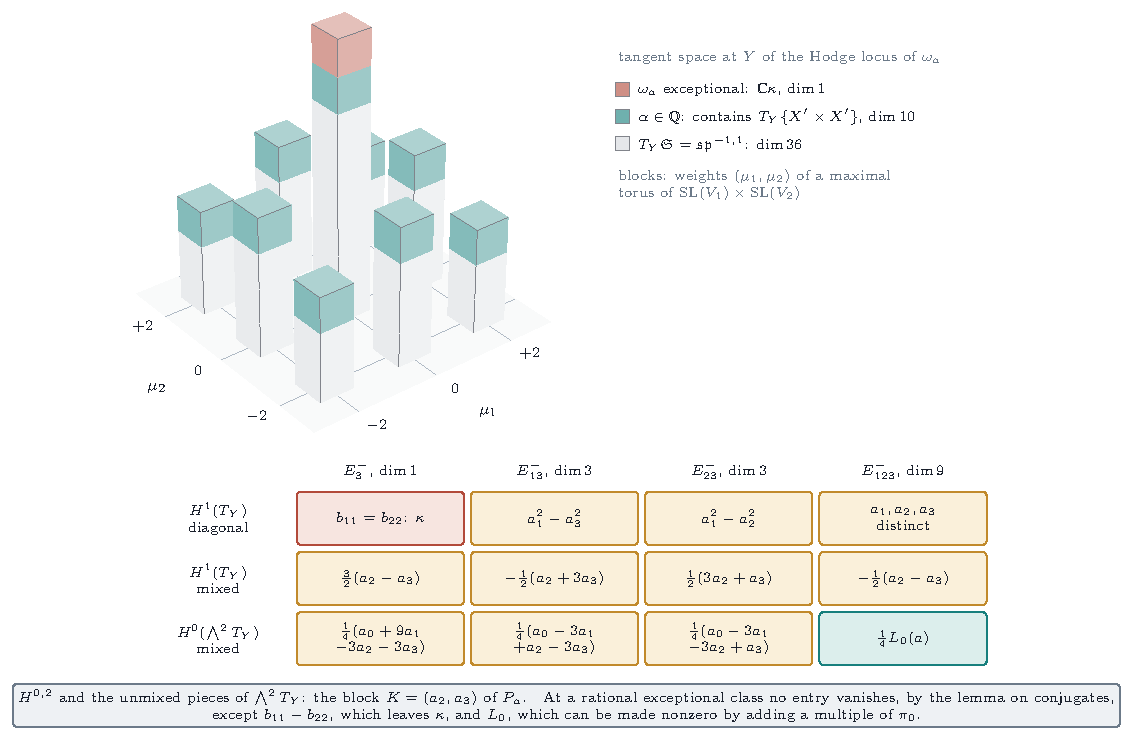
\includegraphics[width=\textwidth]{fig_rigidity}
\caption{\Cref{thm:mumfordrigid}. Top: the tangent space
$\mathfrak{sp}^{-1,1}$ of the Siegel space $\mathfrak{S}$ at
$Y=X_{c}\times X_{c}$, of dimension $36$, split into nine blocks by the
weights of a maximal torus of $\SL(V_{1})\times\SL(V_{2})$, one cube for each
dimension. The tangent space of the Hodge locus of an exceptional class is
the line $\CC\kappa$ of the Mumford curve, in the block of weight $(0,0)$;
for $\alpha\in\QQ$ it contains the tangent space of the diagonal Siegel space,
of dimension $10$ (\Cref{rem:rigidcompare}). Bottom: the scalars of Steps 4
to 6 of the proof on the pieces $E_{J}^{-}$ of $HT^{2}(Y)$; the pieces of
$H^{0,2}$ and the unmixed pieces of $H^{0}(\bigwedge^{2}T_{Y})$ are controlled
by the block $K$ of $P_{a}$ (Steps 3 and 4).}
\label{fig:rigidity}
\end{figure}

\begin{corollary}[No degeneration and no larger family]
\label{cor:nodegeneration}
Let $\omega$ be a rational exceptional class on $X_{c}\times X_{c}$. Every
connected complex analytic family of polarised abelian eightfolds through
$X_{c}\times X_{c}$ on which $\omega$ stays of Hodge type lies, near each
point of the curve, inside the curve $\{X_{t}\times X_{t}:t\in C\}$, which is
compact. In particular no such family degenerates, and on no member of it
other than the CM points of the curve is $\omega$ a combination of products
of divisor classes or of Weil classes of CM fields acting on the member or on
its quotients.
\end{corollary}

\begin{proof}
By \Cref{thm:mumfordrigid}(iii) the Hodge locus of $\omega$ coincides with the
curve in a neighbourhood of every point of the curve, so a connected family
through $Y$ on which $\omega$ stays of Hodge type maps into the curve near
each of its points over the curve; by connectedness and the identity theorem
its image lies in the curve. The curve is compact because $D$ is a division
algebra, so that the arithmetic group of the Shimura curve is cocompact
\cite{Mum69}. Indeed, by \Cref{setup:mumford} the algebra $D$ is definite at
$\sigma_{1}$ and $\sigma_{2}$, so $D\otimes_{F,\sigma_{1}}\RR$ is Hamilton's
quaternions and $D$ is not $M_{2}(F)$: it is a division algebra, split at the
one real place $\sigma_{3}$. The norm one group of an order in $D$, embedded
in $\SL_{2}(\RR)$ through $\sigma_{3}$, is a Fuchsian group of finite
covolume with no parabolic element, since a parabolic $\gamma\ne\pm1$ would
make $\gamma\mp1$ a nonzero nilpotent element of $D$; and a Fuchsian group of
finite covolume without parabolic elements has compact quotient.

For the last assertion: a member of the curve other than a CM point has
Hodge group $G$ (proof of \Cref{cor:mumfordequiv}), and on it $\omega$ lies
outside the span of the products of divisor classes and of the Weil classes
of quotients, by \Cref{prop:mumfordproduct}(ii) and (iii). At a CM point the
class is already algebraic (\Cref{thm:mumfordcm}), and the CM points, being
countably many, do not carry algebraicity to the other members
(\Cref{lem:spreading} needs uncountably many points).
\end{proof}

The same annihilator controls deformations that are not algebraic at all,
and so decides whether the twistor lines along which Markman moves sheaves
in his proof for Weil classes can be used here.

\begin{proposition}[The Hodge locus among all complex tori, and twistor
lines]\label{prop:notwistor}
Let $\omega$ be a rational exceptional class, $Y=X_{c}\times X_{c}$ with
$c\in C$, and $\Lambda=H_{1}(Y,\ZZ)$. Let $\mathcal{T}$ be the space of
complex structures on the real torus $\Lambda_{\RR}/\Lambda$, a complex
manifold of dimension $64$ with tangent space $H^{1}(T_{Y})$ at $Y$, and
$\mathcal{T}_{\omega}\subset\mathcal{T}$ the closed analytic subset on which
$\omega$ is of type $(2,2)$.
\begin{enumerate}[label=\textup{(\roman*)},leftmargin=2.6em,itemsep=2pt]
\item The connected component of $\mathcal{T}_{\omega}$ that contains $Y$ is
  the universal cover $\mathfrak{H}$ of the Mumford curve, the set of
  squares of members of the family, biholomorphic to the upper half plane.
  Every connected complex analytic family of complex tori, algebraic or not,
  through a member of the Mumford family on which $\omega$ stays of Hodge
  type lies in the family.
\item No twistor line through a member of the Mumford family, and no compact
  connected complex curve in $\mathcal{T}$ through it, keeps $\omega$ of
  Hodge type.
\item Nevertheless $\mathcal{T}_{\omega}$ contains twistor lines. The algebra
  $D\otimes_{F,\sigma_{1}}\RR$ is Hamilton's quaternions and acts on
  $V_{\RR}$ through the first factor of $G(\RR)$; for a unit quaternion $j$
  with $j^{2}=-1$, the complex structure $j\oplus j$ on $V_{\RR}\oplus
  V_{\RR}$ makes $\omega$ of type $(2,2)$, and these structures form a twistor
  line. On each factor $\psi(x,jy)$ has signature $(4,4)$, and a member whose
  Mumford--Tate group is $G$ is not an abelian variety. These twistor lines
  lie in components of $\mathcal{T}_{\omega}$ other than $\mathfrak{H}$.
\end{enumerate}
\end{proposition}

\begin{proof}
(i) The complex structures on $\Lambda_{\RR}$ for which all the tensors
invariant under $G$ are of Hodge type are those $J$ with $J^{2}=-1$ in the
real points of $G\cdot\mathbb{G}_{m}$, since a reductive group containing the
homotheties is the stabiliser of its invariant tensors. Let $\mathfrak{H}$ be
the connected component of this closed set that contains $Y$; it is closed in
$\mathcal{T}$ and consists of the $J=1\otimes1\otimes j_{3}$ with
$j_{3}\in\SL_{2}(\RR)$, $j_{3}^{2}=-1$, in the half plane that contains the
structure of $Y$, that is, of the squares of the members of the Mumford
family. At each of its points the first order condition for $\omega$ to stay
of type $(2,2)$ along $\xi\in H^{1}(T_{Y})$ is $\xi\lrcorner\,\omega=0$, as
in the proof of
\Cref{thm:mumfordrigid}(iii), where no polarisation was used, and by
\Cref{thm:mumfordrigid}(i) the solutions form the line $\CC\kappa$ tangent to
$\mathfrak{H}$. So near each of its points $\mathcal{T}_{\omega}$ is the smooth
curve germ of $\mathfrak{H}$, and $\mathfrak{H}$ is open in
$\mathcal{T}_{\omega}$. Being also closed and connected, it is a connected
component. A connected analytic family on which $\omega$ stays of Hodge type
maps into $\mathcal{T}_{\omega}$, hence into $\mathfrak{H}$ once one of its
points does.

(ii) A twistor line is a nonconstant holomorphic image of $\PP^{1}$ in
$\mathcal{T}$. If $\omega$ stayed of Hodge type along one through a point of
$\mathfrak{H}$, or along any compact connected curve through it, the curve
would lie in $\mathfrak{H}$ by (i), and a holomorphic map from a compact
connected curve to the upper half plane is constant.

(iii) At $\sigma_{1}$ the quaternion algebra $D$ is definite
(\Cref{setup:mumford}), so the first factor of $G(\RR)$ is the group of unit
quaternions, and $V_{\RR}$ restricted to it is a module over
$D\otimes_{F,\sigma_{1}}\RR\cong\mathbb{H}$. The unit quaternions $j$ with
$j^{2}=-1$ form a two-sphere, and the complex structures given by left
multiplication by them on a quaternionic vector space form a twistor line.
Each $j$ lies in $G(\RR)$, and so does the circle $\cos\vartheta+j\sin\vartheta$,
which fixes $\omega$; so $\omega$ is of type $(2,2)$. Inside
$V_{1}\otimes V_{2}\otimes V_{3}$ the space $V_{\RR}$ is the fixed space of a
real structure that is quaternionic on the first two factors and real on the
third, so $V_{\RR}=U\otimes V_{3,\RR}$ with $U$ the real form of
$V_{1}\otimes V_{2}$. On $U$ the form $g=\epsilon_{1}\otimes\epsilon_{2}$ is
symmetric and invariant under the compact group of pairs of unit quaternions,
which acts irreducibly on $U\otimes\CC=V_{1}\otimes V_{2}$; so $g$ is
definite. The complex structures of the Mumford family are $1\otimes h$, with
$h$ a complex structure on $V_{3,\RR}$ for which $\epsilon_{3}(\cdot,h\cdot)$
is definite, and $\psi(x,(1\otimes h)y)=g\otimes\epsilon_{3}(\cdot,h\cdot)$ is
definite. For $J=j\otimes1\otimes1$ the form $g(\cdot,(j\otimes1)\cdot)$ is
alternating, $j\otimes1$ being an isometry of $g$ with square $-1$, and
$\psi(x,Jy)=g(\cdot,(j\otimes1)\cdot)\otimes\epsilon_{3}$ is the product of
nondegenerate alternating forms on spaces of dimensions $4$ and $2$; as the
product of two alternating forms on $\RR^{2}$ is the determinant on
$\RR^{2}\otimes\RR^{2}=M_{2}(\RR)$, of signature $(2,2)$, it has signature
$(4,4)$. At a member whose Mumford--Tate group is $G$, the Hodge
classes of degree two on $V_{\RR}\oplus V_{\RR}$ are the forms $\psi\otimes s$
with $s$ a symmetric $2\times2$ matrix, by \Cref{prop:mumfordproduct}(ii), and
the signature of $\psi(\cdot,J\cdot)\otimes s$ is $(4(p+q),4(p+q))$ when $s$ has
signature $(p,q)$, so none is definite, none is a polarisation, and the member
is not an abelian variety. The members of the Mumford family are not on these
lines, since $\psi(x,Jy)$ is definite at the former and of signature $(4,4)$
at the latter, so by (i) the lines lie in other components.
\end{proof}

Markman's proof for Weil classes on abelian fourfolds moves a sheaf along
twistor lines on which its Chern character stays of Hodge type. By
\Cref{prop:notwistor} no such line passes through the square of a member of
the Mumford family: twistor lines on which $\omega$ is of Hodge type exist,
but they carry non-algebraic tori whose Hodge cocharacter lies in a definite
factor of $D$, and they lie in components of the Hodge locus that the Mumford
family never meets. The Kuga--Satake class of \Cref{thm:mumfordks} behaves
differently. The Kuga--Satake construction applies to every Hodge structure
of K3 type on $(T,q_{\lambda})$, so that class stays of Hodge type over the
whole period domain of $(T,q_{\lambda})$, of dimension seven, and not only
along the curve; among the classes attached to the target, it is the only one
for which deformation methods of this kind are not excluded.

The same space $T$ also makes the square a holomorphic symplectic variety,
and this determines what the mechanism of van Geemen and Rapagnetta would
have to supply here. They prove the Hodge conjecture for the general abelian
fourfold of Weil type with trivial discriminant by pulling back the second
Chern class of a hyperk\"ahler sixfold along a map from the fourfold, which
gives an algebraic class of codimension two that is not a product of divisor
classes \cite{vGR26}. For a projective hyperk\"ahler manifold $M$ write
$\sigma_{M}$ for its symplectic form, $q_{M}$ for its Beauville--Bogomolov
form and $T(M)$ for the orthogonal complement of $\NS(M)_{\QQ}$ in
$H^{2}(M,\QQ)$ for $q_{M}$.

\begin{proposition}[The square as a holomorphic symplectic
variety]\label{prop:hksquare}
Let $c\in C$ be a point at which the Mumford--Tate group of $X=X_{c}$ is
$G\cdot\mathbb{G}_{m}$, let $Y=X\times X$, and let $\Psi\in\bigwedge^{2}V$ be
the $G$-invariant bivector dual to $\psi$. For $x\in T$ put
$\iota(x)=(x\otimes1)\Psi$ in $V\otimes V=H^{1}(X,\QQ)\otimes H^{1}(X,\QQ)$, a
K\"unneth component of $H^{2}(Y,\QQ)$, and let $\iota_{2}\colon S^{2}T\to
H^{4}(Y,\QQ)$ be the map $xy\mapsto\iota(x)\cup\iota(y)$. Let $C_{i}\in
S^{2}T_{i}$ be the Casimir element of the trace form of
$\mathfrak{sl}(V_{i})$, and for $\nu\in F$ let
$c_{\nu}=\sum_{i}\sigma_{i}(\nu)C_{i}$, a rational element of $S^{2}T$; for
$\nu\ne0$ it is the element dual to the form $q_{1/\nu}$.
\begin{enumerate}[label=\textup{(\roman*)},leftmargin=2.6em,itemsep=2pt]
\item $\iota$ is an embedding of Hodge structures $T(-1)\to H^{2}(Y,\QQ)$, its
  image is the only irreducible sub-Hodge structure of $H^{2}(Y,\QQ)$ with
  $h^{2,0}=1$, and the holomorphic $2$-form $\sigma_{0}$ spanning its part of
  type $(2,0)$ is symplectic.
\item $\iota_{2}(c_{\nu})=\rho\,\omega_{a}$ with $a_{0}=3\Tr_{F/\QQ}(\nu)$ and
  $\alpha=4\nu-\Tr_{F/\QQ}(\nu)$, in the notation of \Cref{setup:omegaa},
  where $\rho$ is a nonzero rational number independent of $\nu$. So
  $\iota_{2}(c_{\nu})$ is exceptional if and only if $\nu\notin\QQ$, and every
  rational exceptional class is some $\iota_{2}(c_{\nu})$ plus a rational
  multiple of $\pi_{0}$.
\item Let $M$ be a projective hyperk\"ahler manifold and
  $f\colon Y\dashrightarrow M$ a rational map with $f^{*}\sigma_{M}\ne0$. Then
  $f^{*}$ maps $T(M)$ isomorphically onto $\iota(T)$ and is compatible with
  products of classes in $T(M)$; $f$ is generically finite onto a subvariety
  of dimension eight on which $\sigma_{M}$ is generically nondegenerate;
  $b_{2}(M)\ge10$; and $\dim M\ge10$.
\item Suppose in (iii) that $M=S^{[n]}$ is the Hilbert scheme of $n$ points
  on a projective K3 surface $S$, and
  let $q_{\lambda}$ be the form on $T$ that corresponds to the intersection
  form of $S$ on $T(S)=T(M)$ under $\iota^{-1}f^{*}$
  (\Cref{prop:mumfordrm}(iii)). If $\lambda\notin\QQ$, or if the real
  multiplication of $T(S)$ is induced by algebraic cycles on $S\times S$,
  then the Hodge conjecture holds for $Y$.
\end{enumerate}
\end{proposition}

\begin{proof}
(i) The map $\iota$ is $G$-equivariant because $\Psi$ is invariant, and
injective. Its image lies in $S^{2}V$: for $x$ in the symplectic Lie algebra
of $\psi$ one has $(x\otimes1)\Psi=-(1\otimes x)\Psi$, and the exchange of the
two factors carries $(x\otimes1)\Psi$ to $-(1\otimes x)\Psi=(x\otimes1)\Psi$,
because $\Psi$ is alternating. An element $g$ of $G\cdot\mathbb{G}_{m}$
multiplies $\Psi$ by the multiplier $\chi(g)$ of $\psi$, so $(g\otimes g)\iota(x)=
\chi(g)\,\iota(gxg^{-1})$: the map $\iota$ is equivariant for the adjoint
action on $T$ twisted by $\chi$, which is the action defining $T(-1)$. Both
Hodge structures come from the Hodge cocharacter through
$G\cdot\mathbb{G}_{m}$, so $\iota$ is a morphism of Hodge structures from
$T(-1)$. The sub-Hodge structures of $H^{2}(Y,\QQ)$ are its $G$-stable
subspaces, since $\mathbb{G}_{m}$ acts by scalars. Over $\bar{\QQ}$,
$H^{2}(Y)=\bigwedge^{2}(V\otimes\bar{\QQ}^{2})=S^{2}V\oplus(\bigwedge^{2}V)^{\oplus3}$,
and expanding $V\otimes V=\bigotimes_{k}(S^{2}V_{k}\oplus\bigwedge^{2}V_{k})$
gives $\bigwedge^{2}V$ as the sum of the pieces of highest weights $(0,0,0)$,
$(2,2,0)$, $(2,0,2)$, $(0,2,2)$ (an odd number of factors $\bigwedge^{2}V_{k}$)
and $S^{2}V$ as the sum of those of highest weights $(2,2,2)$, $(2,0,0)$,
$(0,2,0)$, $(0,0,2)$. So the isotypic pieces of $H^{2}(Y)$ have these eight
highest weights and dimensions $3,27,27,27,27,3,3,3$. The Hodge cocharacter
acts through $V_{3}$, on which it has one weight of each type, so $S^{2}V_{3}$
has one dimension of type $(2,0)$ and $\bigwedge^{2}V_{3}$ none; the parts of
type $(2,0)$ of the eight pieces have dimensions $0,0,9,9,9,0,0,1$. The last
three pieces occur once, in $S^{2}V$, and are $\iota(T_{1})$, $\iota(T_{2})$,
$\iota(T_{3})$. So an irreducible summand of highest weight $(2,0,2)$ or
$(0,2,2)$ contributes $3$ to $h^{2,0}$, one of weight $(2,2,2)$ contributes
$9$, one of weight $(0,0,2)$ contributes $1$, and the others contribute
nothing. A rational sub-Hodge structure $W$ is stable under the Galois group,
which permutes the highest weights as it permutes the factors, transitively.
So if $W\otimes\bar{\QQ}$ has a summand of weight $(2,2,0)$, $(2,0,2)$ or
$(0,2,2)$, it has summands of all three and $h^{2,0}(W)\ge6$; if it has one of
weight $(2,2,2)$, then $h^{2,0}(W)\ge9$. If $h^{2,0}(W)=1$, therefore,
$W\otimes\bar{\QQ}$ contains the piece $\iota(T_{3})$ of weight $(0,0,2)$,
which has multiplicity one, and with it $\iota(T_{1})$ and $\iota(T_{2})$; so
$W\supseteq\iota(T)$, and $W=\iota(T)$ if $W$ is irreducible. The same
argument shows that $\iota(T)$ is irreducible: a nonzero sub-Hodge structure
of it contains one of the $\iota(T_{i})$ over $\bar{\QQ}$, hence all three.
The part of type $(2,0)$ of $\iota(T)$ is spanned by $\sigma_{0}=\iota(E_{3})$,
where $E_{3}\in\mathfrak{sl}(V_{3})\otimes\CC$ maps $V_{3}^{0,1}$ onto
$V_{3}^{1,0}$. Write $\Psi=\Psi_{1}\otimes\Psi_{2}\otimes\Psi_{3}$ with
$\Psi_{k}\in\bigwedge^{2}V_{k}$ dual to $\epsilon_{k}$, and
$\Psi_{3}=e_{+}\otimes e_{-}-e_{-}\otimes e_{+}$ with $e_{\pm}$ spanning
$V_{3}^{1,0}$ and $V_{3}^{0,1}$. Then $(E_{3}\otimes1)\Psi_{3}$ is a nonzero
multiple of $e_{+}\otimes e_{+}$, so $\sigma_{0}$ is a nonzero multiple of
$\Psi_{1}\otimes\Psi_{2}\otimes e_{+}\otimes e_{+}$: it lies in
$H^{1,0}(X)\otimes H^{1,0}(X)$ and pairs $H^{1,0}$ of the first factor with
$H^{1,0}$ of the second through the nondegenerate form dual to
$\epsilon_{1}\otimes\epsilon_{2}$ on $V_{1}\otimes V_{2}$. So $\sigma_{0}$ has
rank eight: it is a holomorphic symplectic form on $Y$.

(ii) For $x,y\in T$ the class $\iota(x)\cup\iota(y)$ lies in
$H^{2}(X)\otimes H^{2}(X)$ and comes from the tensor
$(x\otimes1)\Psi\otimes(y\otimes1)\Psi$ in $V^{\otimes4}$ by antisymmetrising
its two slots in the first factor of $Y$ and its two slots in the second.
Read it, as in \Cref{setup:omegaa}, as a map from the first-factor slots to
the second-factor slots. Contraction with $\epsilon_{k}$ turns
$\Psi_{k}\otimes\Psi_{k}$ into $\gamma$ times the identity of
$V_{k}\otimes V_{k}$ and, for $x,y\in T_{k}$, the tensor
$(x\otimes1)\Psi_{k}\otimes(y\otimes1)\Psi_{k}$ into $\gamma\,(x\otimes y)$,
with one and the same constant $\gamma\ne0$, since $x$ and $y$ are
antisymmetric for $\epsilon_{k}$ and the two signs cancel. So $\iota_{2}(C_{1})$
corresponds, up to a nonzero constant $\gamma'$ independent of the factor, to
the restriction to $\bigwedge^{2}V$ of $\mathrm{Cas}_{1}\otimes1\otimes1$,
where $\mathrm{Cas}_{1}=\sum_{c}x_{c}\otimes x^{c}=s_{1}-\frac12$ is the
operator of Step 3 of the proof of \Cref{thm:mumfordpowers}, $s_{1}$ the
exchange of the two copies of $V_{1}$. On $\bigwedge^{2}V$ the exchange
$s_{1}$ is $-1$ on $\QQ\theta$ and $U_{23}$ and $+1$ on $U_{12}$ and $U_{13}$,
so $\iota_{2}(C_{1})=\rho\,(3\pi_{0}-\pi_{12}-\pi_{13}+3\pi_{23})$ with
$\rho=-2\gamma'$, and permuting the factors gives the two cyclic permutations
of this identity. Summing with the coefficients $\sigma_{i}(\nu)$ gives
$\iota_{2}(c_{\nu})=\rho\bigl(3\Tr(\nu)\pi_{0}+\sum\sigma_{k}(4\nu-\Tr(\nu))
\pi_{ij}\bigr)$, the sum over $\{i,j,k\}=\{1,2,3\}$ with $i<j$, which is
$\rho\,\omega_{a}$ with the stated $a_{0}$ and $\alpha$. For rational $\nu\ne0$
both $\iota_{2}(c_{\nu})$ and $\omega_{a}$ are rational and nonzero, so
$\rho\in\QQ$. Since
$\Tr(\nu)\in\QQ$, the element $\alpha$ is rational exactly when $\nu$ is; and
$\Tr(\alpha)=\Tr(\nu)$, so $\nu=(\alpha+\Tr(\alpha))/4$ recovers $\nu$ from
any $\alpha\in F$. Two rational classes with the same $\alpha$ differ by a
multiple of $\pi_{0}$, and $\iota_{2}(c_{\nu/\rho})=\omega_{a}$ because
$c_{\nu}$ is linear in $\nu$; so every rational exceptional class is some
$\iota_{2}(c_{\nu})$ plus a rational multiple of $\pi_{0}$. The Casimir element $C_{i}$ is dual to the trace form
on $T_{i}$, so $c_{\nu}$ is dual to $\sum_{i}\sigma_{i}(\nu)^{-1}
\operatorname{tr}(x_{i}y_{i})=q_{1/\nu}(x,y)$.

(iii) Resolve the indeterminacy of $f$ by a sequence of blow-ups along
smooth centres, $\pi\colon\tilde{Y}\to Y$ and $\tilde{f}\colon\tilde{Y}\to M$,
and put $f^{*}=\pi_{*}\tilde{f}^{*}$, a morphism of Hodge structures. The
kernel of $\pi_{*}$ on $H^{2}(\tilde{Y},\QQ)$ is spanned by the classes of
the exceptional divisors, so $\alpha\mapsto\tilde{f}^{*}\alpha-
\pi^{*}f^{*}\alpha$ is a morphism of Hodge structures from $H^{2}(M,\QQ)$ to a
space of Hodge classes. The Hodge structure $T(M)$ is irreducible: a
sub-Hodge structure $W\subseteq T(M)$ with $W^{2,0}=0$ consists of rational
classes of type $(1,1)$, which lie in $\NS(M)_{\QQ}\cap T(M)=0$; if
$W^{2,0}\ne0$, then $\sigma_{M}\in W_{\CC}$, the orthogonal complement of $W$
in $H^{2}(M,\QQ)$ is a sub-Hodge structure orthogonal to $\sigma_{M}$ and
$\bar{\sigma}_{M}$, hence of type $(1,1)$ and contained in $\NS(M)_{\QQ}$,
and $W\supseteq T(M)$. Since $T(M)$ is not spanned by Hodge classes, that
morphism vanishes on it, and $\tilde{f}^{*}\alpha=\pi^{*}f^{*}\alpha$ for
$\alpha\in T(M)$. Because $\tilde{f}^{*}$ is a ring homomorphism and
$\pi_{*}\pi^{*}$ is the identity, $f^{*}(\alpha\beta)=f^{*}\alpha\cup
f^{*}\beta$ for $\alpha,\beta\in T(M)$. The kernel of $f^{*}$ on $T(M)$ is a
sub-Hodge structure not containing $\sigma_{M}$, hence zero, and the image is
irreducible with $h^{2,0}=1$, hence $\iota(T)$ by (i). So $f^{*}\sigma_{M}$ is
a nonzero multiple of $\sigma_{0}$ and has rank eight at every point of $Y$
where $f$ is defined; the rank of a pulled-back form is at most the dimension
of the image, so $f$ is generically finite onto its image $Z$, of dimension
eight, and $\sigma_{M}$ is generically nondegenerate on $Z$. As $M$ is
projective, $b_{2}(M)=\dim T(M)+\dim\NS(M)_{\QQ}\ge9+1$; this excludes the
generalised Kummer varieties, whose second Betti number is seven
\cite{Bea83}. Finally $\dim M\ge\dim Z=8$; suppose that $\dim M=8$. Then
$f$ is dominant, and for $\alpha\in T(M)_{\CC}$ the relation of Fujiki and
Beauville \cite{Bea83,Fuj87} gives
\[
  \int_{Y}(f^{*}\alpha)^{8}=\int_{\tilde{Y}}\tilde{f}^{*}(\alpha^{8})
  =\deg(f)\int_{M}\alpha^{8}=\deg(f)\,c_{M}\,q_{M}(\alpha)^{4},
  \qquad c_{M}>0 .
\]
Write $f^{*}\alpha=\iota(x)$ with $x=x_{1}+x_{2}+x_{3}\in T_{\CC}$ and
$N_{i}=-\det x_{i}$. The form $x\mapsto q_{M}((f^{*})^{-1}\iota(x))$ is
invariant under $G$, so it is $q_{\lambda}(x,x)=
\sum_{i}\sigma_{i}(\lambda)\operatorname{tr}(x_{i}^{2})=
2\sum_{i}\sigma_{i}(\lambda)N_{i}$ for some $\lambda\in F^{\times}$ by
\Cref{prop:mumfordrm}(iii). On the other side, in a basis $(e_{i})$ of
$V$ one has $\iota(x)=\sum_{i,j}M_{ij}\,e_{i}^{(1)}\wedge e_{j}^{(2)}$, with
$M$ the product of the matrix of $x$ and the constant invertible matrix of
$\Psi$, and the $2$-forms $e_{i}^{(1)}\wedge e_{j}^{(2)}$ commute, so
$\iota(x)^{8}=8!\det(M)\prod_{i}e_{i}^{(1)}\wedge e_{i}^{(2)}$ is $8!\det(x)$
times a fixed volume form, and
$\det(x_{1}\otimes1\otimes1+1\otimes x_{2}\otimes1+1\otimes1\otimes
x_{3})=\Delta(N_{1},N_{2},N_{3})^{2}$ with
$\Delta=N_{1}^{2}+N_{2}^{2}+N_{3}^{2}-2N_{1}N_{2}-2N_{1}N_{3}-2N_{2}N_{3}$;
this is also the product of the eight numbers $\pm r_{1}\pm r_{2}\pm r_{3}$,
where $\pm r_{i}$ are the eigenvalues of $x_{i}$ and $r_{i}^{2}=N_{i}$. The
$N_{i}$ are algebraically independent functions on $T_{\CC}$, so the two
expressions for $\int_{Y}(f^{*}\alpha)^{8}$ would make $\Delta^{2}$ a nonzero
constant multiple of the fourth power of the linear form
$\sum_{i}\sigma_{i}(\lambda)N_{i}$, and then, by unique factorisation,
$\Delta$ a multiple of its square. But $\Delta$ is a nondegenerate
ternary quadratic form, hence irreducible. So $\dim M\ne8$, and since the
dimension of a hyperk\"ahler manifold is even, $\dim M\ge10$.

(iv) By \cite{Bea83} the map $H^{2}(S,\QQ)\to H^{2}(S^{[n]},\QQ)$ induced by
the universal subscheme $Z_{n}\subset S\times S^{[n]}$ is injective, carries
the intersection form to the Beauville--Bogomolov form, and has
$H^{2}(S^{[n]},\QQ)=H^{2}(S,\QQ)\oplus\QQ\delta$ with $\delta$ algebraic, so
$T(M)=T(S)$. Let $\Delta_{T}$ be the K\"unneth component in $T(S)\otimes
T(S)$ of the class of the diagonal of $S$; it is algebraic, being the class
of the diagonal minus $[\mathrm{pt}\times S]$, $[S\times\mathrm{pt}]$ and
$\sum_{r}d_{r}\times d_{r}^{\vee}$ over dual bases of $\NS(S)_{\QQ}$. Its image
under the correspondence $Z_{n}\times Z_{n}$, pulled back along the diagonal
of $M$, is the class $\sum_{a}e_{a}\cup e_{a}^{\vee}$ over dual bases of
$T(S)$ for the intersection form, which is therefore algebraic on $M$, and by
(iii) its image under $f^{*}$ is $\iota_{2}$ of the element of $S^{2}T$ dual
to $q_{\lambda}$, that is $\iota_{2}(c_{1/\lambda})$, an algebraic class on
$Y$. If $\lambda\notin\QQ$ it is exceptional by (ii). If instead the real
multiplication is algebraic, apply it to the first factor of $\Delta_{T}$:
for $b\in F$ the class $\sum_{a}(m_{b}e_{a})\cup e_{a}^{\vee}$ is algebraic,
and its image is $\iota_{2}(c_{b/\lambda})$, which is exceptional for
$b\notin\QQ\lambda$. In both cases \Cref{lem:oneexceptional} makes every
Hodge class in $H^{2}(X)\otimes H^{2}(X)$ algebraic; the Hodge classes in the
other K\"unneth components of $H^{4}(Y,\QQ)$ are products of divisor classes,
as at the end of the proof of \Cref{thm:mumfordks}; and the Hodge classes of
$Y$ form a ring generated in degrees two and four (proof of
\Cref{cor:mumfordequiv}). So every Hodge class of $Y$ is algebraic.
\end{proof}

\begin{remark}[The mechanism of van Geemen and
Rapagnetta]\label{rem:hkroute}
By \Cref{prop:hksquare}(ii) the exceptional classes are, up to rational
multiples of $\pi_{0}$, the classes $\iota_{2}(c_{\nu})$ with $\nu\notin\QQ$,
the images of the elements dual to the forms $q_{\lambda}$, $\lambda=1/\nu$,
on the part $\iota(T)$ of $H^{2}(Y)$ generated by the symplectic class; the
form with $\lambda$ rational gives a product of divisor classes. They are the
analogues for $(Y,\sigma_{0})$ of the dual Beauville--Bogomolov class, whose
pull-back is what \cite{vGR26} uses. By part (iii), a transfer of that
argument needs a projective hyperk\"ahler manifold of dimension at least ten with
transcendental part $T(-1)$, such as $S_{\mu}^{[n]}$ with $n\ge5$ for a
surface $S_{\mu}$ of \Cref{thm:mumfordks}, and a rational map from $Y$ onto a
symplectic subvariety of dimension eight. For $M=S_{\mu}^{[n]}$ the form of
(iv) is $q_{\mu/e^{2}}$ for the $e\in F^{\times}$ with $\iota^{-1}f^{*}=m_{e}$
on $T(S_{\mu})=T$, so $\lambda\notin\QQ$ for every such map as soon as
$\mu\notin\QQ^{\times}F^{\times2}$. No such map is known. It would give an
algebraic cycle on $S_{\mu}\times X\times X$ inducing an isomorphism of
$T(S_{\mu})$ onto $\iota(T)\subset H^{1}(X)\otimes H^{1}(X)$, a correspondence
of the kind that the Kuga--Satake class supplies in the proof of
\Cref{thm:mumfordks}; so this route is the Kuga--Satake route in geometric
form rather than an independent one. By (iii), maps to K3 surfaces and to
hyperk\"ahler eightfolds cannot serve.
\end{remark}

\begin{theorem}[A numerical criterion for the Mumford classes]
\label{thm:mumfordnumerical}
Let $c\in C$, $Y=X_{c}\times X_{c}$, $\omega=\omega_{a}$ a rational
exceptional class with $L_{0}(a)\ne0$, and $E$ a perfect complex on $Y$ with
$\ch(E)=N\omega$, $N\ne0$, and no other component.
\begin{enumerate}[label=\textup{(\roman*)},leftmargin=2.6em,itemsep=2pt]
\item $\dim\Ext^{2}(E,E)\ge119$.
\item If $\dim\Ext^{2}(E,E)=119$, then $\operatorname{ev}_{E}\colon
  HT^{2}(Y)\to\Ext^{2}(E,E)$ is surjective with kernel $\CC\kappa$, and
  $\sigma_{E}$ is injective. Conversely, if $\sigma_{E}$ is injective, then
  $\operatorname{ev}_{E}$ has rank $119$ and kernel $\CC\kappa$, and $E$
  extends to first order along the curve.
\item If some such $E$ at one point $c$ has $\dim\Ext^{2}(E,E)=119$, then
  $\omega_{t}$ is algebraic for every $t\in C$, the Hodge conjecture holds for
  $X_{t}\times X_{t}$ for every $t$, and $B(W\times_{C}W)$ holds.
\item At every CM point $c$ some perfect complex $E$ on $Y$ has
  $\ch(E)=N\omega$ for some $N\ne0$ and no other component.
\end{enumerate}
\end{theorem}

\begin{proof}
(i) and (ii). By the square $\sigma_{E}\circ\operatorname{ev}_{E}=
(\,\cdot\,)\lrcorner\,\ch(E)$ of \Cref{setup:criterion}, $\ker
\operatorname{ev}_{E}\subseteq\Ann_{HT^{2}}(\omega)=\CC\kappa$ by
\Cref{thm:mumfordrigid}(ii), so $\operatorname{ev}_{E}$ has rank at least
$119$, which is (i). If $\dim\Ext^{2}(E,E)=119$, then
$\operatorname{ev}_{E}$ is onto, its kernel has dimension one and lies in
$\CC\kappa$, so equals it; and $\sigma_{E}(\operatorname{ev}_{E}(x))=
N\,x\lrcorner\,\omega$ vanishes only for $x\in\CC\kappa=\ker
\operatorname{ev}_{E}$, so $\sigma_{E}$ is injective on
$\image\operatorname{ev}_{E}=\Ext^{2}(E,E)$. Conversely, if $\sigma_{E}$ is
injective, then $\sigma_{E}(\operatorname{ev}_{E}(\kappa))=N\kappa\lrcorner
\,\omega=0$ forces $\operatorname{ev}_{E}(\kappa)=0$, so the kernel is
$\CC\kappa$ and the rank is $119$; and $\operatorname{ev}_{E}$ restricted to
$H^{1}(T_{Y})$ is the obstruction map \cite{Tod09}, which therefore vanishes
at $\kappa$, so that $E$ extends to first order along the curve.

(iii) By (ii) $\sigma_{E}$ is injective. The Chern character of $E$ is
$N\omega$, a flat section of Hodge type over the whole of $C$, so
\Cref{thm:BF} applies to every infinitesimal deformation of $Y$ inside
$W\times_{C}W\to C$. The proof of \Cref{thm:semiregclosure} then applies word
for word, with the stack of perfect complexes on the fibres of $W\times_{C}
W\to C$ \cite{Lie06} in place of that of $\cA\to\cS$, or the analytic
Kuranishi germ if $\Ext^{<0}(E,E)\ne0$: it is smooth over $C$ at $[E]$, its
image contains a nonempty open subset $U\subseteq C$, and for $t\in U$ a
perfect complex $E_{t}$ on $X_{t}\times X_{t}$ in the same connected
component has $\ch(E_{t})=N\omega_{t}$, so $\omega_{t}$ is algebraic, and by
\Cref{lem:oneexceptional} so are both exceptional classes. Since $U$ is
uncountable, \Cref{cor:mumfordequiv} gives the rest.

(iv) By \Cref{thm:mumfordcm} there is $\xi\in\CH^{2}(Y)_{\QQ}$ with class
$\omega$, and the argument of \Cref{prop:ktheory} gives $E$: the Chern
character is an isomorphism $K_{0}(Y)_{\QQ}\to\CH^{*}(Y)_{\QQ}$
\cite[Ex.~15.2.16(b) and Cor.~18.3.2]{Ful98}, so $\xi=\ch(u)$ for a unique
$u$, and $Nu$ is the class of a perfect complex for a suitable $N$.
\end{proof}

Part (iii) is the Mumford analogue of \Cref{thm:p2numerical}(iii): one object,
at one point, and one number, which is $119$ here and $2n(2n-1)$ for a Weil
family. For a Weil family that number is attained by no object
(\Cref{thm:p2false}), because an object attaining it would have to deform to
non-algebraic tori; the classes here are rigid, so that argument does not
apply (\Cref{rem:p2prime}). The objects of (iv) exist, and the criterion
asks that one of them, or another representative of the same class in
$K_{0}$, attain the bound of (i). The rigidity of \Cref{thm:mumfordrigid} is no obstacle:
semiregularity moves an object along the Hodge locus of its Chern character,
and the curve is exactly that locus, so a semiregular object would propagate
along the curve and nowhere else, which is all that is needed.

\begin{corollary}[Bounded data at CM points]\label{cor:mumfordbounded}
Fix a relatively ample line bundle on $W\times_{C}W\to C$, and let $\omega$ be
a rational exceptional class. The following are equivalent.
\begin{enumerate}[label=\textup{(\alph*)},leftmargin=2.6em,itemsep=2pt]
\item $\omega_{t}$ is algebraic for every $t\in C$; equivalently, by
  \Cref{lem:oneexceptional} and \Cref{cor:mumfordequiv}, the Hodge conjecture
  holds for $X_{t}\times X_{t}$ for every $t\in C$.
\item There are a finite set $\Phi$ of pairs $(\underline{P},\underline{q})$,
  each a tuple of Hilbert polynomials with a tuple of rational numbers of the
  same length, and infinitely many points $c\in C$ at each of which
  $\omega_{c}=\sum_{i}q_{i}[Z_{i}]$ for subschemes $Z_{i}\subset X_{c}\times
  X_{c}$ with Hilbert polynomials $P_{i}$, for some $(\underline{P},
  \underline{q})\in\Phi$.
\end{enumerate}
In particular the classes are algebraic on every member as soon as they are
represented at infinitely many CM points by cycles of bounded degree.
\end{corollary}

\begin{proof}
For a pair $(\underline{P},\underline{q})$ let $\Sigma_{\underline{P},
\underline{q}}\subseteq C$ be the set of points at which $\omega$ is
represented with these data. The proof of \Cref{thm:closedlocus} applies
verbatim to $(W\times_{C}W,C,\omega)$, as in \Cref{lem:spreading}, and shows
that each $\Sigma_{\underline{P},\underline{q}}$ is Zariski closed. If (b)
holds, then, $\Phi$ being finite, one pair of $\Phi$ serves at infinitely
many points, so its $\Sigma$ is an infinite closed subset of the irreducible
curve $C$, hence $C$, and (a) holds. If (a) holds, $C$ is the union of the
countably many $\Sigma_{\underline{P},\underline{q}}$, and $C$ is
uncountable, so one of
them is infinite, hence equal to $C$; then (b) holds with $\Phi$ that one
pair and every point of $C$.
\end{proof}

The proof of \Cref{thm:mumfordcm} represents the classes at every CM point,
through Markman's theorem for abelian fourfolds \cite{Mar25a} and the ring
generated by divisor classes and pull-backs of Hodge classes of $X_{c}$ along
homomorphisms $X_{c}\times X_{c}\to X_{c}$, but with no control of degree;
isogenies between CM members, which move CM points along their Hecke orbits,
do not bound the degree either. By
\Cref{cor:mumfordbounded} such a bound, at infinitely many CM points, is
equivalent to the target; without it the CM points, being countably many,
say nothing about a very general member (\Cref{lem:spreading} needs
uncountably many points).

The next proposition says which endomorphisms those pull-backs have to use.
At a CM point the fourfold is of Weil type, its two Hodge classes of degree
four that are not products of divisor classes form its Weil line, and the
exceptional classes of the square are out of reach of everything built from
that line with the Weil field alone: they need the real multiplication by the
totally real quartic algebra of Rosati-fixed endomorphisms, and all of it.

\begin{proposition}[The Weil structure at a CM point, and what the cycles
must use]\label{prop:cmsource}
Let $c\in C$ be a CM point, $X=X_{c}$, $Y=X\times X$, and let $e_{w}$,
$w\in\{\pm1\}^{3}$, be a weight basis of $V=H^{1}(X,\CC)$ for the Hodge torus
$T$ of $X$, as in the proof of \Cref{thm:mumfordcm}, normalised so that
$\psi(e_{w},e_{-w})=\pm1$, with $e^{(1)}_{w}$, $e^{(2)}_{w}$ its two copies in
$H^{1}(Y,\CC)$. Let $T_{+}$ be the set of the four weights with an even
number of entries $-1$, let $T_{-}=-T_{+}$ be the set of the other four, let
$t_{\pm}=\prod_{w\in T_{\pm}}e_{w}\in H^{4}(X,\CC)$, the factors in a fixed
order, and let $\dagger$ be the Rosati involution of $\theta$ on
$\End^{0}(X)$. For $\varphi\in\End^{0}(X)$ write $\varphi_{w}$ for its
eigenvalue on $e_{w}$.
\begin{enumerate}[label=\textup{(\roman*)},leftmargin=2.6em,itemsep=2pt]
\item $T_{+}$ and $T_{-}$ are the only sets of four weights with sum zero
  that contain no pair of opposite weights, and $\Hdg^{2}(X)\otimes\CC$ is
  the direct sum of the span of the products of divisor classes and of
  $\CC t_{+}\oplus\CC t_{-}$. The elements of $\End^{0}(X)$ with
  $\varphi_{w}$ constant on $T_{+}$ and constant on $T_{-}$ form an imaginary
  quadratic field $k_{c}$; $(X,k_{c},\theta)$ is of $(k_{c},-1,2)$-Weil type,
  and its Weil line is $\HW(X)=(\CC t_{+}\oplus\CC t_{-})\cap H^{4}(X,\QQ)$.
  The fixed algebra $K_{c}^{+}$ of $\dagger$ consists of the elements with
  $\varphi_{w}=\varphi_{-w}$ for every $w$; it is a product of totally real
  fields of total degree four, and $\End^{0}(X)=K_{c}^{+}\otimes_{\QQ}k_{c}$.
\item For $\varphi,\psi\in\End^{0}(X)$ let $f_{\varphi,\psi}^{*}$ be the ring
  homomorphism $H^{*}(X,\QQ)\to H^{*}(Y,\QQ)$ that sends $e\in H^{1}(X,\QQ)$
  to $\mathrm{pr}_{1}^{*}\varphi^{*}e+\mathrm{pr}_{2}^{*}\psi^{*}e$; for
  $\varphi,\psi\in\End(X)$ it is the pull-back along the homomorphism
  $\varphi\circ\mathrm{pr}_{1}+\psi\circ\mathrm{pr}_{2}\colon Y\to X$, and
  every homomorphism $Y\to X$ is of this form. For a $\QQ$-subalgebra
  $R\subseteq\End^{0}(X)$ let $\Sigma_{R}\subseteq\Hdg^{2}(Y)$ be the
  $\QQ$-span of the products of two divisor classes of $Y$ and of the classes
  $f_{\varphi,\psi}^{*}\HW(X)$ with $\varphi,\psi\in R$. Then
  $\Sigma_{k_{c}}=\Sigma_{\QQ}$, the span obtained from the maps
  $(x,y)\mapsto ax+by$ alone, has dimension $110$ and meets the span of
  $\pi_{0},\pi_{12},\pi_{13},\pi_{23}$ in the plane of the classes with
  $a_{1}=a_{2}=a_{3}$; it contains no exceptional class.
\item For a $\QQ$-subalgebra $R\subseteq\End^{0}(X)$ the following are
  equivalent: \textup{(a)} $\Sigma_{R}$ contains an exceptional class;
  \textup{(b)} $\Sigma_{R}=\Hdg^{2}(Y)$, which has dimension $132$;
  \textup{(c)} $R$ separates the weights of $T_{+}$, that is, for any two
  distinct $w,w'\in T_{+}$ some $\varphi\in R$ has
  $\varphi_{w}\ne\varphi_{w'}$; equivalently, $R$ and $k_{c}$ generate
  $\End^{0}(X)$. In particular $\Sigma_{K_{c}^{+}}=\Hdg^{2}(Y)$, while
  $\Sigma_{R}$ contains no exceptional class if $R$ is a proper subalgebra
  of $K_{c}^{+}$ or a subalgebra of $k_{c}$.
\end{enumerate}
\end{proposition}

\begin{proof}
(i) The four weights $d_{1}=(1,1,1)$, $d_{2}=(1,-1,-1)$, $d_{3}=(-1,1,-1)$,
$d_{4}=(-1,-1,1)$ of $T_{+}$ have sum zero, and any three of them are
linearly independent, so every linear relation among them is a multiple of
$d_{1}+d_{2}+d_{3}+d_{4}=0$. A set of four weights containing no opposite
pair contains exactly one of $d_{i}$, $-d_{i}$ for each $i$, say
$\varepsilon_{i}d_{i}$, and has sum zero only if
$\sum_{i}\varepsilon_{i}d_{i}=0$, that is, if all $\varepsilon_{i}$ are
equal: the set is $T_{+}$ or $T_{-}$. The Hodge classes of $X$ of degree
four, tensored with $\CC$, are spanned by the monomials $\prod_{w\in S}e_{w}$
over the sets $S$ of four weights with sum zero (proof of
\Cref{thm:mumfordcm}); the divisor classes are spanned by the four monomials
$e_{w}e_{-w}$ of weight zero and degree two, their products are the six
monomials of the sets that are unions of two opposite pairs, and the two
remaining sets are $T_{+}$ and $T_{-}$.

The torus $T$ is defined over $\QQ$, so the Galois group of $\bar{\QQ}$ acts
linearly on its character lattice and permutes the set of the eight weights
of $V$. A linear map that permutes the weights carries opposite pairs to
opposite pairs and sets with sum zero to sets with sum zero, hence carries
$\{T_{+},T_{-}\}$ to itself. Over $\bar{\QQ}$ the algebra
$\End^{0}(X)\otimes\bar{\QQ}=\End_{T}(V_{\bar{\QQ}})$ consists of the
diagonal matrices $\sum_{w}x_{w}p_{w}$ in the weight basis, $p_{w}$ the
projection to the weight space of $w$, and $\gamma\in\Gal(\bar{\QQ}/\QQ)$
acts by $\gamma(\sum_{w}x_{w}p_{w})=\sum_{w}\gamma(x_{w})p_{\gamma w}$,
because $\gamma$ carries the weight space of $w$ to that of $\gamma w$. As
$\psi$ is $T$-invariant, $\psi(e_{w},e_{w'})=0$ unless $w'=-w$, so the
adjoint of $\sum_{w}x_{w}p_{w}$ for $\psi$, which is the Rosati involution,
is $\sum_{w}x_{-w}p_{w}$. The subalgebra $A_{W}$ of the diagonal matrices
that are constant on $T_{+}$ and on $T_{-}$, and the subalgebra $A^{+}$ of
those with $x_{w}=x_{-w}$ for all $w$, are therefore stable under the Galois
group and under $\dagger$; so $k_{c}=A_{W}\cap\End^{0}(X)$ and
$K_{c}^{+}=A^{+}\cap\End^{0}(X)$ are $\QQ$-forms of $A_{W}$ and $A^{+}$, of
dimensions $2$ and $4$, and $K_{c}^{+}$ is the fixed algebra of $\dagger$.
On $A_{W}$ the involution $\dagger$ exchanges the two scalars. The Rosati
involution is positive: $\Tr(xx^{\dagger})>0$ for $x\ne0$, with $\Tr$ the
trace on $V$ \cite[Section~5.1]{BL04}. If $k_{c}$ were not a field it would
contain the idempotent $p_{+}=\sum_{w\in T_{+}}p_{w}$, and
$\Tr(p_{+}p_{+}^{\dagger})=\Tr(p_{+}p_{-})=0$; so $k_{c}$ is a quadratic
field on which $\dagger$ is the nontrivial automorphism. If $k_{c}$ were
real, $x=\sqrt{d}\in k_{c}$ would satisfy $x^{\dagger}=-x$ and
$\Tr(xx^{\dagger})=-\Tr(x^{2})=-8d<0$. So $k_{c}$ is imaginary quadratic and
$\dagger$ is complex conjugation on it, which is condition (iii) of
\Cref{def:weiltype}. The eigenspaces of $k_{c}\otimes\CC$ on $V$ are
$V_{\pm}=\bigoplus_{w\in T_{\pm}}\CC e_{w}$. The Hodge decomposition of $V$
is the eigenspace decomposition of the Hodge cocharacter, which takes values
in the diagonal torus $T_{\CC}\cdot\mathbb{G}_{m}$, so every $e_{w}$ is of
pure type $(1,0)$ or $(0,1)$, and $t_{+}$ is of type $(p,4-p)$ with
$p=\dim(V_{+}\cap H^{1,0}(X))$. Since $t_{+}$ is a Hodge class, $p=2$: each
eigenvalue of $\sqrt{-d}$ has multiplicity two on $H^{1,0}(X)$, which is
condition (ii) of \Cref{def:weiltype}, and condition (i) is $\dim X=4$. The
Weil line of \Cref{def:weilline} is
$(\bigwedge^{4}V_{+}\oplus\bigwedge^{4}V_{-})\cap H^{4}(X,\QQ)
=(\CC t_{+}\oplus\CC t_{-})\cap H^{4}(X,\QQ)$; it has dimension two by
\Cref{prop:weilline}(i), so it is a rational complement of the products of
divisor classes in $\Hdg^{2}(X)$. The algebra $K_{c}^{+}$ is commutative and
semisimple, being a subalgebra of $\End^{0}(X)$, whose complexification is
commutative, and its trace form $\Tr(xy)=\Tr(xy^{\dagger})$ is positive
definite; so every factor field $E$ of $K_{c}^{+}$ has
$\Tr_{E/\QQ}(x^{2})>0$ for $x\ne0$ and is totally real. Finally the
multiplication map $K_{c}^{+}\otimes_{\QQ}k_{c}\to\End^{0}(X)$ is an
isomorphism, because over $\bar{\QQ}$ it is the isomorphism
$\bar{\QQ}^{\{\text{opposite pairs}\}}\otimes\bar{\QQ}^{\{T_{+},T_{-}\}}
\to\bar{\QQ}^{\{\text{weights}\}}$ induced by the bijection that sends a
weight to the pair and the tetrahedron containing it, a bijection because
the two weights of a pair lie in different tetrahedra, $T_{-}$ being $-T_{+}$.

(ii) Extend the notation: for diagonal $\varphi,\psi\in\End^{0}(X)\otimes\CC$
with entries $\varphi_{w}$, $\psi_{w}$ let $f_{\varphi,\psi}^{*}$ be the ring
homomorphism $H^{*}(X,\CC)\to H^{*}(Y,\CC)$ with
$e_{w}\mapsto\varphi_{w}e^{(1)}_{w}+\psi_{w}e^{(2)}_{w}$; for
$\varphi,\psi\in\End^{0}(X)$ this is the map of the statement, since
$\varphi^{*}e_{w}=\varphi_{w}e_{w}$, and every homomorphism $Y\to X$ is
$\varphi\circ\mathrm{pr}_{1}+\psi\circ\mathrm{pr}_{2}$ for its restrictions
$\varphi,\psi$ to the two factors. Then
\begin{equation}\label{eq:pullbacktet}
  f_{\varphi,\psi}^{*}t_{\pm}
  =\prod_{w\in T_{\pm}}\bigl(\varphi_{w}e^{(1)}_{w}+\psi_{w}e^{(2)}_{w}\bigr)
  =\sum_{S\subseteq T_{\pm}}\pm\Bigl(\prod_{w\in S}\varphi_{w}\Bigr)
  \Bigl(\prod_{w\in T_{\pm}\setminus S}\psi_{w}\Bigr)\,
  e^{(1)}_{S}\,e^{(2)}_{T_{\pm}\setminus S},
\end{equation}
where $e^{(1)}_{S}e^{(2)}_{T\setminus S}$ is the product of the $e^{(1)}_{w}$,
$w\in S$, and the $e^{(2)}_{w}$, $w\in T\setminus S$, taken in the order of
$T$, and the sign is that of the shuffle. We call these $32$ products the
tetrahedron monomials. The Hodge classes of $Y$ of degree four, tensored with
$\CC$, are spanned by the monomials of weight zero in the sixteen classes
$e^{(i)}_{w}$ (proof of \Cref{thm:mumfordcm}). Such a monomial whose four
weights contain an opposite pair is the product of two monomials of weight
zero and degree two, that is, of two divisor classes: there are four of the
form $e^{(1)}_{w}e^{(2)}_{w}e^{(1)}_{-w}e^{(2)}_{-w}$ and $96$ with two
distinct opposite pairs and a choice of copy for each of the four weights.
A weight repeated twice, $2w+w'+w''=0$, forces $w'=w''=-w$, so the remaining
monomials have four distinct weights with no opposite pair, and by (i) they
are the tetrahedron monomials. Hence $\dim\Hdg^{2}(Y)=132$, the products of
divisor classes span the $100$ monomials of the first two kinds, and the
tetrahedron monomials form a basis of the quotient $\Xi$ of
$\Hdg^{2}(Y)\otimes\CC$ by the span of the products of divisor classes. Two
distinct weights of a tetrahedron $T$ differ in exactly two coordinates, and
for $S=\{a,b\}\subseteq T$ the complement $T\setminus S$ has the same set of
differing coordinates, because $a+b$ and the sum of the complement are
opposite. Writing $D(a,b)\subseteq\{1,2,3\}$ for the set of coordinates in
which two weights differ, the six tetrahedron monomials of $T$ with two
factors from each copy fall into three pairs
$\{e^{(1)}_{S}e^{(2)}_{T\setminus S},e^{(1)}_{T\setminus S}e^{(2)}_{S}\}$,
indexed by the two-element set $D(S)=D(T\setminus S)$.

For $\varphi,\psi\in k_{c}\otimes\CC=A_{W}$, with values $\varphi_{\pm}$,
$\psi_{\pm}$ on $T_{\pm}$, \eqref{eq:pullbacktet} reads
$f_{\varphi,\psi}^{*}t_{\pm}=\sum_{k=0}^{4}\varphi_{\pm}^{k}\psi_{\pm}^{4-k}
s_{\pm,k}$, where $s_{\pm,k}$ is the sum, with the signs of
\eqref{eq:pullbacktet}, of the tetrahedron monomials of $T_{\pm}$ with $k$
factors from the first copy. Conversely the classes
$(a\,\mathrm{pr}_{1}+b\,\mathrm{pr}_{2})^{*}t_{\pm}$ for five values of $a/b$
span the $s_{\pm,k}$, a Vandermonde matrix being invertible. Since
$\HW(X)\otimes\CC=\CC t_{+}\oplus\CC t_{-}$, the complexifications of
$\Sigma_{k_{c}}$ and of $\Sigma_{\QQ}$ are both spanned by the products of
divisor classes and the ten classes $s_{\pm,k}$, which are supported on
disjoint nonempty sets of tetrahedron monomials; so
$\Sigma_{k_{c}}=\Sigma_{\QQ}$ has dimension $100+10=110$.

For the four $\pi$ we use the description of \Cref{setup:omegaa}. Fix a
total order on the weights, and for an endomorphism $A$ of
$H^{2}(X,\CC)={\textstyle\bigwedge^{2}}V$ let
\[
  c(A)=\sum_{a<b}A(e_{a}e_{b})\otimes(e_{a}e_{b})^{\vee}
  \in H^{2}(X)\otimes H^{2}(X)
\]
be its class, where $(e_{a}e_{b})^{\vee}$ is the dual basis for the form
${\textstyle\bigwedge^{2}}\psi$. As
${\textstyle\bigwedge^{2}}\psi(e_{a}e_{b},e_{c}e_{d})
=\psi(e_{a},e_{c})\psi(e_{b},e_{d})-\psi(e_{a},e_{d})\psi(e_{b},e_{c})$
vanishes unless $\{c,d\}=\{-a,-b\}$, we have
$(e_{a}e_{b})^{\vee}=\chi(a)\chi(b)\,e_{-a}e_{-b}$ with
$\chi(w)=\psi(e_{w},e_{-w})=\pm1$, the two factors in the order matching
$(a,b)$. Let $s_{t}$, $t=1,2,3$, be the involution of
$V\otimes V=\bigotimes_{u=1}^{3}(V_{u}\otimes V_{u})$ that exchanges the two
factors $V_{t}$. The three $s_{t}$ commute, and $s_{1}s_{2}s_{3}$ is the
exchange of the two slots of $V\otimes V$, which is $-1$ on
${\textstyle\bigwedge^{2}}V$; so each $s_{t}$ preserves
${\textstyle\bigwedge^{2}}V$, on which $s_{1}s_{2}s_{3}=-1$, and
${\textstyle\bigwedge^{2}}V$ is the sum of the four joint eigenspaces with
eigenvalues $(\varepsilon_{1},\varepsilon_{2},\varepsilon_{3})$ of product
$-1$: these are $\CC\theta={\textstyle\bigwedge^{2}}V_{1}\otimes
{\textstyle\bigwedge^{2}}V_{2}\otimes{\textstyle\bigwedge^{2}}V_{3}$ for
$(-1,-1,-1)$ and $U_{ij}=S^{2}V_{i}\otimes S^{2}V_{j}\otimes
{\textstyle\bigwedge^{2}}V_{k}$ for $\varepsilon_{i}=\varepsilon_{j}=1$,
$\varepsilon_{k}=-1$. The projection onto the eigenspace of
$(\varepsilon_{1},\varepsilon_{2},\varepsilon_{3})$ is
$\prod_{t}(1+\varepsilon_{t}s_{t})/2$, which by the relation
$s_{1}s_{2}s_{3}=-1$ equals
$(1+\varepsilon_{1}s_{1}+\varepsilon_{2}s_{2}+\varepsilon_{3}s_{3})/4$. So
\[
  \pi_{0}=c\Bigl(\frac{1-s_{1}-s_{2}-s_{3}}{4}\Bigr),\qquad
  \pi_{12}=c\Bigl(\frac{1+s_{1}+s_{2}-s_{3}}{4}\Bigr),
\]
and $\pi_{13}$, $\pi_{23}$ likewise, with the plus signs at $s_{1},s_{3}$
and at $s_{2},s_{3}$. Let $a^{t}$ be the weight $a$ with its $t$-th
coordinate changed; then $s_{t}(e_{a}e_{b})=e_{a}e_{b}$ if $t\notin D(a,b)$
and $s_{t}(e_{a}e_{b})=e_{a^{t}}e_{b^{t}}$ if $t\in D(a,b)$. Under the
K\"unneth map to $H^{4}(Y,\CC)$ the term of the pair $\{a,b\}$ in $c(s_{t})$
is, up to sign, the monomial $e^{(1)}_{a'}e^{(1)}_{b'}e^{(2)}_{-a}e^{(2)}_{-b}$
with $\{a',b'\}=\{a,b\}$ if $t\notin D(a,b)$ and $\{a',b'\}=\{a^{t},b^{t}\}$
otherwise. If $t\notin D(a,b)$, or $D(a,b)=\{t\}$, in which case $a^{t}=b$,
or $D(a,b)=\{1,2,3\}$, in which case $b=-a$ and the monomial is
$e^{(1)}_{a^{t}}e^{(1)}_{-a^{t}}e^{(2)}_{-a}e^{(2)}_{a}$, the monomial
contains an opposite pair and is a product of two divisor classes. In the
remaining case $D(a,b)=\{t,t'\}$ with $t'\ne t$; then $b=a^{tt'}$, and the
four weights $a^{t}$, $b^{t}=a^{t'}$, $-a$, $-b=a^{t''}$, where
$\{t,t',t''\}=\{1,2,3\}$, are pairwise non-opposite, since any two of them
differ in exactly two coordinates, and they have sum zero, because
$a^{t}+b^{t}$ and $a+b$ agree outside the $t$-th coordinate, where both
vanish. So
\[
  m_{ab}=\chi(a)\chi(b)\,e^{(1)}_{a^{t}}e^{(1)}_{b^{t}}e^{(2)}_{-a}e^{(2)}_{-b},
  \qquad t=\min D(a,b),
\]
is a tetrahedron monomial with $D(a^{t},b^{t})=D(-a,-b)=D(a,b)$, and since
$s_{t'}(e_{a}e_{b})=e_{a^{t'}}e_{b^{t'}}=e_{b^{t}}e_{a^{t}}=-e_{a^{t}}e_{b^{t}}$,
the term of the pair in $c(s_{t'})$ is $-m_{ab}$, while its term in
$c(s_{t''})$ is a product of divisor classes. For each two-element set $D$
put $u_{D}=\sum_{D(a,b)=D}m_{ab}$, a sum over the four pairs with difference
set $D$: two of these pairs lie in each tetrahedron and $a^{t}$ lies in the
other one, so $u_{D}$ has two monomials in each tetrahedron, all with
coefficients $\pm1$, and the three $u_{D}$ are supported on disjoint sets of
monomials; the two monomials of $u_{D}$ in $T$ are those of the pair of
$T$ indexed by $D$. In $\Xi$ this gives $c(1)\equiv0$,
$c(s_{1})\equiv u_{12}+u_{13}$, $c(s_{2})\equiv-u_{12}+u_{23}$,
$c(s_{3})\equiv-u_{13}-u_{23}$, hence
\begin{equation}\label{eq:pimodulo}
  \pi_{0}\equiv0,\quad
  \pi_{12}\equiv\tfrac12(u_{13}+u_{23}),\quad
  \pi_{13}\equiv\tfrac12(u_{12}-u_{23}),\quad
  \pi_{23}\equiv-\tfrac12(u_{12}+u_{13}),
\end{equation}
and $\omega_{a}\equiv\frac12\bigl((a_{2}-a_{3})u_{12}+(a_{1}-a_{3})u_{13}
+(a_{1}-a_{2})u_{23}\bigr)$ in $\Xi$: on the monomials of the pair of
$T_{\pm}$ indexed by $\{1,2\}$, $\{1,3\}$, $\{2,3\}$ the class $\omega_{a}$
has coefficients of absolute values $|a_{2}-a_{3}|/2$, $|a_{1}-a_{3}|/2$,
$|a_{1}-a_{2}|/2$.

Now suppose that $\omega_{a}\in\Sigma_{\QQ}\otimes\CC$. Its image in $\Xi$
is a combination of the $s_{\pm,k}$, and since every monomial of
$\omega_{a}$ has two factors from each copy, only $s_{+,2}$ and $s_{-,2}$
occur: $\omega_{a}\equiv x\,s_{+,2}+y\,s_{-,2}$. On the six monomials of
$T_{+}$ the right side has coefficients of absolute value $|x|$. So the
three differences $a_{2}-a_{3}$, $a_{1}-a_{3}$, $a_{1}-a_{2}$ have a common
absolute value $r$, and as $a_{1}-a_{3}=(a_{1}-a_{2})+(a_{2}-a_{3})$,
$r\in\{0,2r\}$; hence $r=0$ and $a_{1}=a_{2}=a_{3}$. Conversely the classes
with $a_{1}=a_{2}=a_{3}$ are the combinations of $\pi_{0}$ and
$\pi_{12}+\pi_{13}+\pi_{23}$, which are invariant under $\Sp(V,\psi)$ and so
are combinations of the products of divisor classes $\psi_{11}\psi_{22}$ and
$\psi_{12}^{2}$ (proof of \Cref{prop:mumfordrm}(ii)); they lie in
$\Sigma_{\QQ}$. An exceptional class
has for $(a_{1},a_{2},a_{3})$ the three distinct conjugates of an element of
$F\setminus\QQ$ (\Cref{lem:conjugates}), so it does not lie in
$\Sigma_{\QQ}$.

(iii) We first show that (c) is equivalent to $R$ and $k_{c}$ generating
$\End^{0}(X)$, and that $R$ separates the weights of $T_{+}$ if and only if
it separates those of $T_{-}$. For $\varphi\in\End^{0}(X)$ the eigenvalue on
$e_{-w}$ is $\varphi_{-w}=(\varphi^{\dagger})_{w}$; since $\End^{0}(X)$ is a
product of CM fields on which $\dagger$ is complex conjugation, and every
embedding of a CM field into $\CC$ commutes with complex conjugation,
$\varphi_{-w}=\bbar{\varphi_{w}}$. Hence $\varphi_{w}=\varphi_{w'}$ if and
only if $\varphi_{-w}=\varphi_{-w'}$, and $R$ separates $T_{+}$ if and only
if it separates $T_{-}$. The elements of $k_{c}$ are constant on each
tetrahedron and separate the two, and a subalgebra of
$\bar{\QQ}^{\{\text{weights}\}}$ containing the constants is the algebra of
functions constant on the blocks of the partition it induces; so $R$
separates $T_{+}$ exactly when $R\cdot k_{c}\otimes\bar{\QQ}$ separates all
eight weights, that is, when $R\cdot k_{c}=\End^{0}(X)$.

(c) implies (b). If $R$ separates $T_{+}$, then $R\otimes\CC$ maps onto
$\CC^{T_{+}}$ under $\varphi\mapsto(\varphi_{w})_{w\in T_{+}}$, so the
entries $\varphi_{w}$, $\psi_{w}$, $w\in T_{+}$, are eight independent
coordinates on the image of $(R\otimes\CC)^{2}$. The sixteen coefficients in
\eqref{eq:pullbacktet} are distinct monomials in these coordinates, hence
linearly independent functions of $(\varphi,\psi)\in(R\otimes\CC)^{2}$; so
no nonzero linear form on the span of the sixteen tetrahedron monomials of
$T_{+}$ vanishes on all $f_{\varphi,\psi}^{*}t_{+}$, and these classes span
that space. The same holds for $T_{-}$, and with the $100$ products of
divisor classes this is all of $\Hdg^{2}(Y)\otimes\CC$. The map
$(\varphi,\psi)\mapsto f_{\varphi,\psi}^{*}t_{\pm}$ is polynomial and
$R\times R$ is Zariski dense in $(R\otimes\CC)^{2}$, so a linear form
vanishing on its values at rational pairs vanishes on all values, and
finitely many pairs $\varphi,\psi\in R$ give the same span. The $\QQ$-span of
the rational classes $f_{\varphi,\psi}^{*}\HW(X)$, $\varphi,\psi\in R$, and
of the products of divisor classes is then a $\QQ$-subspace of
$\Hdg^{2}(Y)$ whose complexification is the whole space, hence is
$\Hdg^{2}(Y)$.

(b) implies (a), as $\Hdg^{2}(Y)$ contains the exceptional classes.

(a) implies (c). Suppose that two distinct weights $u,u'\in T_{+}$ have
$\varphi_{u}=\varphi_{u'}$ for every $\varphi\in R$, and let $v,v'$ be the
other two weights of $T_{+}$. In \eqref{eq:pullbacktet} the sets
$S=\{u,v\}$ and $S'=\{u',v\}$ then have the same coefficient for every
$\varphi,\psi\in R$, up to the signs of the shuffles, which do not depend on
$\varphi,\psi$. Hence every class in $\Sigma_{R}\otimes\CC$ has coefficients
of equal absolute value on the tetrahedron monomials $e^{(1)}_{S}e^{(2)}_{T_{+}\setminus S}$ and $e^{(1)}_{S'}e^{(2)}_{T_{+}\setminus S'}$, the products
of divisor classes involving no tetrahedron monomial. The pairs
$\{S,T_{+}\setminus S\}$ and $\{S',T_{+}\setminus S'\}$ are different
partitions of $T_{+}$, so $D(S)\ne D(S')$, and for an exceptional class
$\omega_{a}$ in $\Sigma_{R}$ two of the three numbers $|a_{2}-a_{3}|$,
$|a_{1}-a_{3}|$, $|a_{1}-a_{2}|$ would be equal. Each of the six resulting
equations, $a_{2}-a_{3}=\pm(a_{1}-a_{3})$ and the four others, is a linear
relation $c_{1}a_{1}+c_{2}a_{2}+c_{3}a_{3}=0$ with rational coefficients not
all equal, which \Cref{lem:conjugates} forbids for the conjugates of an
element of $F\setminus\QQ$. So (a) fails, and this proves the equivalence.

For the last assertions: $K_{c}^{+}\otimes\bar{\QQ}$ consists of all
functions on the opposite pairs, and $T_{+}$ meets every pair once, so
$K_{c}^{+}$ separates $T_{+}$; a proper subalgebra $R$ of $K_{c}^{+}$ has
$R\otimes\bar{\QQ}$ a proper subalgebra of the functions on the four pairs,
which identifies two pairs and hence two weights of $T_{+}$; and a
subalgebra of $k_{c}$ is constant on $T_{+}$.
\end{proof}

\Cref{fig:cmcube} draws the weights of part (i), and \Cref{fig:cmsource}
the Hodge classes of parts (ii) and (iii).

\begin{figure}[tbp]
\centering
  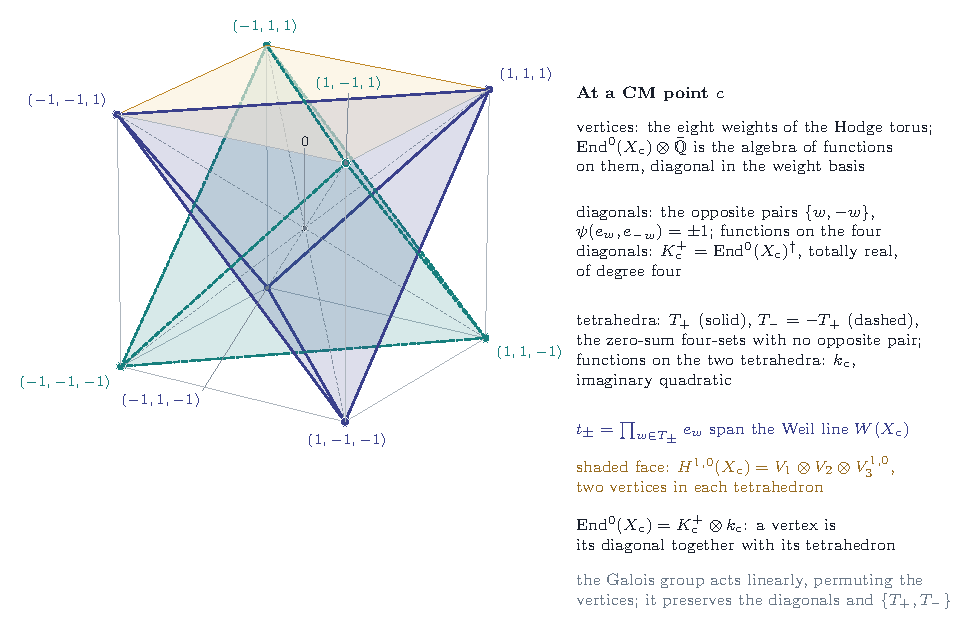
\includegraphics[width=0.96\textwidth]{fig_cmcube}
\caption{\Cref{prop:cmsource}(i). The eight weights $(\pm1,\pm1,\pm1)$ of the
Hodge torus at a CM point are the vertices of a cube. The four diagonals are
the pairs of opposite weights, paired by the polarisation; the two inscribed
tetrahedra $T_{+}$ (an even number of entries $-1$) and $T_{-}=-T_{+}$ are
the only zero-sum four-sets without an opposite pair, and $t_{\pm}=\prod_{w\in
T_{\pm}}e_{w}$ span the Weil line. The Galois group acts by linear maps
permuting the vertices, so it preserves the diagonals and the pair of
tetrahedra: the functions constant on the tetrahedra form the imaginary
quadratic Weil field $k_{c}$, those constant on the diagonals the totally real
quartic algebra $K_{c}^{+}$ of Rosati-fixed endomorphisms, and
$\End^{0}(X_{c})=K_{c}^{+}\otimes k_{c}$ because a vertex is determined by
its diagonal and its tetrahedron.}
\label{fig:cmcube}
\end{figure}

\begin{figure}[tbp]
\centering
  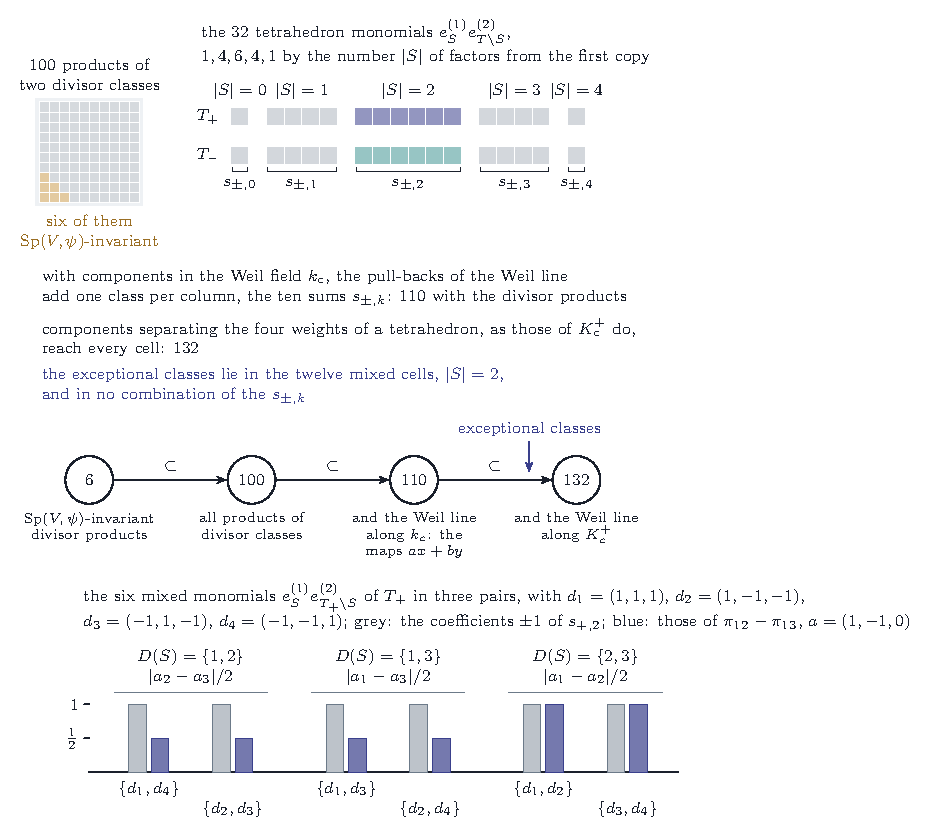
\includegraphics[width=\textwidth]{fig_cmsource}
\caption{\Cref{prop:cmsource}(ii) and (iii). Top: the $132$ Hodge classes of
degree four on the square at a CM point, one cell per monomial of weight
zero. The $100$ products of divisor classes are the cells with an opposite
pair; the $32$ tetrahedron monomials $e^{(1)}_{S}e^{(2)}_{T\setminus S}$ are
arranged by tetrahedron and by the number $|S|$ of factors from the first
copy. Pull-backs of the Weil line along homomorphisms with components in
$k_{c}$ add only the ten symmetric sums $s_{\pm,k}$, one per column, giving
$110$; components separating the four weights of a tetrahedron, as those of
$K_{c}^{+}$ do, separate the monomials and give all $132$. Bottom: on the six
mixed monomials of one tetrahedron, grouped in the three pairs by the
coordinates in which the two weights of $S$ differ, the symmetric sum
$s_{+,2}$ has coefficients $\pm1$ throughout, while an exceptional class
$\omega_{a}$ has coefficients of absolute value $|a_{2}-a_{3}|/2$,
$|a_{1}-a_{3}|/2$, $|a_{1}-a_{2}|/2$, drawn for $\pi_{12}-\pi_{13}$; two
equal absolute values would be a linear relation among the conjugates of an
irrational element of $F$.}
\label{fig:cmsource}
\end{figure}

The CM points fall into two kinds, according to whether the fourfold is
simple; at the points of the second kind the real multiplication comes from
the fixed cubic field $F$.

\begin{lemma}[Split CM points]\label{lem:splitcm}
Let $c\in C$ be a CM point, and let $L\subset D$ be the quadratic extension
of $F$ whose norm one torus $\Res_{F/\QQ}\ker(\Nm_{L/F})$ is the Hodge group
of $X_{c}$ (proof of \Cref{thm:mumfordcm}). Then $L$ is a CM field, and the
following are equivalent: \textup{(a)} $X_{c}$ is not simple; \textup{(b)}
$K_{c}^{+}$ is not a field; \textup{(c)} $L=Fk$ for an imaginary quadratic
field $k\subseteq L$. In that case $k_{c}\cong k$, $K_{c}^{+}\cong\QQ\times F$,
and $X_{c}$ is isogenous to $E\times B$, where $E$ is an elliptic curve with
complex multiplication by $k$ and $B$ is an abelian threefold of CM type on
which the factor $F$ of $K_{c}^{+}$ acts, a real multiplication by $F$; the
Weil line $\HW(X_{c})$ lies in $H^{1}(E)\otimes H^{3}(B)$. At every other CM
point $K_{c}^{+}$ is a totally real quartic field. Points of the second kind
exist for infinitely many $k$: for every imaginary quadratic field $k$ such
that $k\otimes_{\QQ}F_{v}$ is a field at each finite place $v$ of $F$ at
which $D$ is ramified.
\end{lemma}

\begin{proof}
Write $T$ for the Hodge group. By \Cref{prop:cmsource}(i), $\End^{0}(X_{c})
=K_{c}^{+}\otimes k_{c}$ is a product of CM fields on which $\dagger$ is
complex conjugation, and $T$ lies in the centraliser of $\End^{0}(X_{c})$,
which over $\bar{\QQ}$ is the diagonal torus, and in $\Sp(V,\psi)$; so
$T(\RR)$ lies in the compact group of the $x\in(\End^{0}(X_{c})\otimes\RR)
^{\times}$ with $xx^{\dagger}=1$. If $L\otimes_{F,\sigma}\RR$ were
$\RR\times\RR$ at a real place $\sigma$, the factor of $T(\RR)$ at $\sigma$
would be the norm one group of $\RR\times\RR$ over $\RR$, which is not
compact. Hence $L\otimes_{F,\sigma}\RR=\CC$ at each real place, and $L$ is a
CM field.

Over $\bar{\QQ}$, $T=\prod_{\sigma}T_{\sigma}$ with $T_{\sigma}
=\ker(\Nm_{L/F})\otimes_{F,\sigma}\bar{\QQ}$ the diagonal torus of
$\SL_{2}(\bar{\QQ})=(D\otimes_{F,\sigma}\bar{\QQ})^{1}$ for the decomposition
$L\otimes_{F,\sigma}\bar{\QQ}=\bar{\QQ}\times\bar{\QQ}$ by the two embeddings
of $L$ over $\sigma$, one of them chosen and called $\tau_{\sigma}$, the
other $\bar{\tau}_{\sigma}$. The factor $V_{\sigma}$ of
$V=\bigotimes_{\sigma}V_{\sigma}$ (\Cref{setup:mumford}) has the weights
$\tau_{\sigma}$ and $\bar{\tau}_{\sigma}=\tau_{\sigma}^{-1}$ on $T_{\sigma}$,
with eigenvectors $v_{\sigma,\pm}$, and $e_{w}=\bigotimes_{\sigma}
v_{\sigma,w_{\sigma}}$. An element $\gamma$ of the Galois group carries
$V_{\sigma}$ to $V_{\gamma\sigma}$ and $v_{\sigma,+}$ to
$v_{\gamma\sigma,\varepsilon_{\gamma}(\sigma)}$, where
$\varepsilon_{\gamma}(\sigma)=1$ if $\gamma\tau_{\sigma}=\tau_{\gamma\sigma}$
and $-1$ if $\gamma\tau_{\sigma}=\bar{\tau}_{\gamma\sigma}$; so it acts on
the weights by $(\gamma w)_{\gamma\sigma}=\varepsilon_{\gamma}(\sigma)
w_{\sigma}$.

If $L=Fk$, then $\operatorname{Hom}(L,\bar{\QQ})=\operatorname{Hom}(F,\bar{\QQ})
\times\operatorname{Hom}(k,\bar{\QQ})$ with the Galois group acting on both
factors, and with $\tau_{\sigma}=\sigma\otimes\iota_{0}$ for a fixed
embedding $\iota_{0}$ of $k$ the sign $\varepsilon_{\gamma}(\sigma)
=\varepsilon_{\gamma}$ does not depend on $\sigma$: it is $1$ if $\gamma$
fixes $k$ and $-1$ otherwise. Then $\gamma$ permutes the coordinates of a
weight and changes all its signs when it moves $k$. It preserves each
tetrahedron if it fixes $k$ and exchanges the two otherwise, so
$k_{c}\otimes\bar{\QQ}=\bar{\QQ}^{\{T_{+},T_{-}\}}$ is the algebra of the
Galois set $\operatorname{Hom}(k,\bar{\QQ})$, and $k_{c}\cong k$. It carries
the pair $\{\pm(1,1,1)\}$ to itself, so the projection $p_{E}$ onto
$\CC e_{(1,1,1)}\oplus\CC e_{(-1,-1,-1)}$ lies in $\End^{0}(X_{c})$, and by
Poincar\'e reducibility $X_{c}$ is isogenous to $E\times B$ with
$H^{1}(E,\CC)$ the image of $p_{E}$, of dimension two, so $E$ is an
elliptic curve, on whose $H^{1}$ the field $k_{c}$ acts by two conjugate
scalars: $E$ has complex multiplication by $k$. The threefold $B$ has
$\End^{0}(B)\otimes\bar{\QQ}$ containing the diagonal algebra of the six
remaining weights, of dimension $6=2\dim B$, so $B$ is of CM type. Each of
the six remaining weights has exactly one coordinate different from the
other two, and $\gamma$ carries the opposite pair of the weight with
distinguished coordinate $t$ to the pair with distinguished coordinate
$\gamma t$; so the Galois set of the four opposite pairs is the fixed point
$\{\pm(1,1,1)\}$ together with a copy of $\operatorname{Hom}(F,\bar{\QQ})$,
and $K_{c}^{+}\cong\QQ\times F$, the factor $\QQ$ acting on $H^{1}(E)$ and
the factor $F$ on $H^{1}(B)$. Finally $T_{+}$ consists of $(1,1,1)$ and
three weights of $B$, and $T_{-}$ of $(-1,-1,-1)$ and three weights of $B$,
so $t_{\pm}\in H^{1}(E)\otimes H^{3}(B)$ and $\HW(X_{c})$ lies there. This
proves that (c) implies (a) and (b), with the asserted structure.

$X_{c}$ is simple exactly when $\End^{0}(X_{c})=K_{c}^{+}\otimes k_{c}$ is a
field, and since every factor field $E'$ of $K_{c}^{+}$ is totally real,
$E'\otimes k_{c}$ is a field; so (a) and (b) are equivalent. Suppose (b).
Then the Galois group does not act transitively on the four opposite pairs,
whose algebra is $K_{c}^{+}$. It acts transitively on the three
coordinates, as on the embeddings of $F$, so some $\gamma$ permutes them
cyclically. For each coordinate $t$ the four pairs fall into two sets of
two, according to the value of the coordinate $t$ on the representatives in
$T_{+}$, and this assigns the three coordinates bijectively to the three
partitions of the four pairs into two sets of two, compatibly with the
Galois action, which preserves or exchanges $T_{+}$ and $T_{-}$. So the
permutation of the pairs induced by $\gamma$ has order divisible by three,
hence equal to three: it is a cycle of length three and fixes exactly one
pair. The orbits of the Galois group on the pairs are therefore either one
orbit or two, of sizes one and three, and by hypothesis some pair
$\{w,-w\}$ is fixed: $\gamma w=\delta_{\gamma}w$ with
$\delta_{\gamma}=\pm1$ for every $\gamma$. Replace the choice of
$\tau_{\sigma}$ by $\tau'_{\sigma}=\tau_{\sigma}$ if $w_{\sigma}=1$ and
$\tau'_{\sigma}=\bar{\tau}_{\sigma}$ if $w_{\sigma}=-1$; for the new choice
$w$ becomes $(1,1,1)$, and the new signs are
$\varepsilon'_{\gamma}(\sigma)=\varepsilon_{\gamma}(\sigma)w_{\sigma}
w_{\gamma\sigma}=\delta_{\gamma}$ for all $\sigma$. So $\gamma$ carries the
set $\Phi=\{\tau'_{\sigma}\}$ of three embeddings of $L$ to $\Phi$ if
$\delta_{\gamma}=1$ and to $\bar{\Phi}$ if $\delta_{\gamma}=-1$. The map
$\gamma\mapsto\delta_{\gamma}$ is a character of the Galois group; it is
nontrivial, for otherwise $\Phi$ would be a Galois stable set of three of the
six embeddings and $L$ would not be a field; and complex conjugation carries
every embedding $\tau$ of the CM field $L$ to $\bar{\tau}$, hence $\Phi$ to
$\bar{\Phi}$, so the quadratic field $k$ cut out by the character is
imaginary. Let $\iota_{0}$, $\bar{\iota}_{0}$ be the embeddings of $k$, with
$\iota_{0}$ fixed by the kernel of the character. Then $\tau\mapsto(\tau|_{F},
\iota_{0}\text{ if }\tau\in\Phi\text{ and }\bar{\iota}_{0}\text{ otherwise})$
is a Galois equivariant bijection $\operatorname{Hom}(L,\bar{\QQ})\to
\operatorname{Hom}(F,\bar{\QQ})\times\operatorname{Hom}(k,\bar{\QQ})$, so
$L\cong F\otimes_{\QQ}k$, that is, $L=Fk$ for a copy of $k$ in $L$, which is
(c). At a CM point where (c) fails, $K_{c}^{+}$ is therefore a field, quartic
and totally real by \Cref{prop:cmsource}(i).

Existence. Let $k$ be imaginary quadratic. By the theorem of Albert, Brauer,
Hasse and Noether \cite[\S1.5]{PR94}, the CM field $Fk$ splits $D$, and so
embeds in $D$ over $F$, exactly when $Fk\otimes_{F}F_{v}$ is a field at
every place $v$ of $F$ at which $D$ is ramified, a quadratic extension of a
local field splitting the local quaternion division algebra. At the two real
places where $D$ is definite this holds because $k$ is imaginary, and at the
finite ramified places it is the hypothesis. Given the finitely many
residue characteristics $p$ of these places, choose for each a quadratic
extension $k_{p}$ of $\QQ_{p}$ not contained in $F_{v}$ for any $v$ above
$p$: this is possible since the completions $F_{v}$ above $p$ have degrees
over $\QQ_{p}$ adding up to three, so at most one of them contains a
quadratic extension of $\QQ_{p}$, and then exactly one, while $\QQ_{p}$ has
at least three. Infinitely many imaginary quadratic fields $k$ have the
completions $k_{p}$ at these $p$, and for them
$F_{v}\otimes_{\QQ_{p}}k_{p}$ is a field. For such $k$ let
$T_{k}=\Res_{F/\QQ}\ker(\Nm_{Fk/F})\subset G$, a maximal torus with
$T_{k}(\RR)$ compact. A compact subgroup of $G(\RR)$ fixes a point $x$ of the
symmetric space of $G(\RR)$, and the stabiliser of $x$ is the centraliser of
$h_{x}(\mathbb{S})$; so $h_{x}(\mathbb{S})$ centralises $T_{k}(\RR)$, which
is Zariski dense in $T_{k}$, and lies in $T_{k}(\RR)$. The Hodge group of
the fibre $X_{c}$ over the image $c$ of $x$ is the smallest $\QQ$-subgroup
of $G$ containing $h_{x}(U(1))$, so it lies in $T_{k}$; it has rank three
(proof of \Cref{thm:mumfordcm}), so it equals $T_{k}$, and $c$ is a CM
point with $L=Fk$.
\end{proof}

\begin{remark}[What the degree bound has to control]\label{rem:cmsource}
\leavevmode
\begin{enumerate}[label=\textup{(\arabic*)},leftmargin=2.6em,itemsep=3pt]
\item Markman's theorem \cite{Mar25a}, which the proof of
  \Cref{thm:mumfordcm} invokes, produces the cycles on $X_{c}$ through its
  Weil structure for $k_{c}$. \Cref{prop:cmsource} says that this structure
  is blind to the exceptional classes of the square: everything obtained
  from the Weil line and from divisors by pull-back along homomorphisms with
  components in $k_{c}$, in particular along the maps $(x,y)\mapsto ax+by$,
  and by products, spans $110$ of the $132$ Hodge classes and misses every
  exceptional class; and a representation of an exceptional class by
  pull-backs of the Weil line and products of divisors must use
  homomorphisms whose components, with $k_{c}$, generate the whole
  endomorphism algebra. At a CM point the exceptional classes are thus a
  statement about the real multiplication $K_{c}^{+}$, as they are at a
  general point about the real multiplication by $F$
  (\Cref{prop:mumfordrm}).
\item For $\varphi,\psi\in\End(X_{c})$ and a cycle $Z$ of codimension two on
  $X_{c}$, the degree $\int_{Y}f_{\varphi,\psi}^{*}[Z]\cup\theta_{Y}^{6}$
  is, by \eqref{eq:pullbacktet} applied to the monomials of $[Z]$, a
  polynomial of degree four in the eigenvalues $\varphi_{w}$, $\psi_{w}$,
  which are algebraic integers. For cycles of this shape the bound of
  \Cref{cor:mumfordbounded} therefore asks, at infinitely many CM points,
  for endomorphisms with bounded eigenvalues whose components generate
  $\End^{0}(X_{c})$ over $k_{c}$. Only finitely many algebraic integers of
  degree at most eight have bounded conjugates, so the same finitely many
  minimal polynomials would have to occur at infinitely many points. At
  the split points of \Cref{lem:splitcm} the algebra $K_{c}^{+}=\QQ\times F$
  does not depend on the point and the real multiplication is by $F$ on the
  threefold factor; the representation of the proof of \Cref{thm:mumfordcm}
  then uses, besides elements of $F$, the isogeny $X_{c}\to E\times B$, a
  cycle representing the Weil line of $E\times B$ in
  $H^{1}(E)\otimes H^{3}(B)$, and divisor classes, and these three are what
  varies with the point.
\item At a split point the Weil line is a Hodge class in $H^{1}(E)\otimes
  H^{3}(B)$, a correspondence between an elliptic curve with complex
  multiplication by $k$ and a CM threefold with real multiplication by $F$,
  and its algebraicity is again Markman's theorem for the fourfold
  $E\times B$. A construction of that correspondence with a degree bounded
  independently of $k$, together with a bound on the isogeny and on the
  divisor classes, would give the target through \Cref{cor:mumfordbounded}.
  We do not have one.
\end{enumerate}
\end{remark}

\begin{remark}[Routes to the Mumford target]\label{rem:bypassaudit}
We list the routes to the Mumford target that avoid the Lefschetz standard
conjecture, with what is known about each; \Cref{fig:bypass} summarises
them.
\begin{enumerate}[label=\textup{(\arabic*)},leftmargin=2.6em,itemsep=2pt]
\item \emph{Degeneration.} Closed off: the base is compact and the Hodge
  locus is the base (\Cref{cor:nodegeneration}), so no family on which
  $\omega$ stays of Hodge type approaches the boundary, and there is no limit
  mixed Hodge structure to specialise to.
\item \emph{Deformation into a larger Hodge locus}, on which $\omega$ would
  become a product of divisor classes or a Weil class, hence algebraic by a
  known theorem, and could then be carried back. Closed off by
  \Cref{thm:mumfordrigid}(iii), already to first order.
\item \emph{Hochschild deformations}: twisting $D^{b}(Y)$ by a $B$-field or a
  Poisson bivector, as in the gerby and noncommutative deformations used for
  Weil classes. Closed off: an object with $\ch(E)=N\omega$ extends along no
  direction of $HH^{2}(Y)$ except that of the curve
  (\Cref{cor:mumfordsplit}(i)).
\item \emph{Constructions from line bundles}: cones, tensor products, duals,
  pull-backs and push-forwards along homomorphisms, and Fourier--Mukai
  functors whose kernels are built in the same way. Closed off at every point
  of the curve: everything so built has a Chern character invariant under the
  Lefschetz group, and the exceptional classes are not
  (\Cref{thm:lefschetzclosure}).
\item \emph{Twistor and hyperholomorphic deformation}, the mechanism of
  Markman's proof for Weil classes: move a sheaf along twistor lines on which
  its Chern character stays of Hodge type. Closed off on the square: no
  twistor line through a member of the Mumford family keeps $\omega$ of Hodge
  type, and the twistor lines that do keep it of Hodge type carry
  non-algebraic tori and lie in other components of the Hodge locus
  (\Cref{prop:notwistor}).
\item \emph{Specialisation.} The class is algebraic at every CM point
  (\Cref{thm:mumfordcm}), on every power of $X_{c}$ \cite[Theorem~1.3]{Li26};
  this suffices exactly when the degrees are bounded
  (\Cref{cor:mumfordbounded}), and no bound is known. The cycles that
  represent the class at a CM point must use the real multiplication by the
  Rosati-fixed algebra $K_{c}^{+}$, all of it; the Weil structure of the
  fourfold, with which Markman's theorem produces its cycles, reaches $110$
  of the $132$ Hodge classes and none of the exceptional ones
  (\Cref{prop:cmsource}, \Cref{rem:cmsource}).
\item \emph{Reduction modulo $p$.} At every closed point of every reduction
  of the curve the class is a $\QQ_{\ell}$-combination of algebraic cycles
  (\Cref{prop:modp}), by Li's theorem \cite[Theorem~1.1]{Li26}; this
  suffices, with no lifting step, exactly when the Hilbert data of the cycles
  are bounded on a Zariski dense set of closed points of the arithmetic model
  (\Cref{thm:modpdensity}), and no bound is known.
\item \emph{Semiregularity.} Reduced to one dimension count at one CM point
  (\Cref{thm:mumfordnumerical}); an object attaining it has large odd
  self-extensions (\Cref{thm:mumfordprofile}), is not built from line
  bundles (\Cref{prop:mumforddivisor}) and splits only in a constrained way
  (\Cref{cor:mumfordsplit}); no such object is known.
\item \emph{Kuga--Satake.} Reduced to the Kuga--Satake class of one K3 surface
  of Picard number thirteen (\Cref{thm:mumfordks}), which the known cases of
  the Kuga--Satake Hodge conjecture do not reach (\Cref{rem:mumfordks}). Its
  geometric form is the mechanism of van Geemen and Rapagnetta \cite{vGR26},
  pull-back of the dual Beauville--Bogomolov class of a hyperk\"ahler
  manifold: up to multiples of $\pi_{0}$, the exceptional classes are exactly
  such twisted dual forms of the part of $H^{2}$ of the square generated by
  its symplectic class, and a rational map onto a
  symplectic subvariety of some $S_{\mu}^{[n]}$, $n\ge5$, would suffice;
  K3 surfaces and hyperk\"ahler eightfolds cannot serve
  (\Cref{prop:hksquare}, \Cref{rem:hkroute}).
\item \emph{Motivated classes.} Every Hodge class on an abelian variety is
  motivated \cite[Th\'eor\`eme~0.6.2]{And96b}, so $\omega_{t}$ is motivated for
  every $t$; a motivated class is algebraic once the Lefschetz involutions of
  the auxiliary varieties are (\Cref{prop:lefmot}). Along the family the
  auxiliary variety that suffices is $W\times_{C}W$
  (\Cref{thm:lefschetzpropagation}), and its Lefschetz standard conjecture is
  equivalent to the target (\Cref{cor:mumfordequiv}): the route moves the
  problem and does not shorten it.
\end{enumerate}
Five of the ten routes are closed off by theorems. Of the other five, two
work at special points only, the CM points and the closed points of the
reductions modulo $p$, and each suffices exactly when a degree bound holds;
two are reduced to a single object, one Kuga--Satake class or one perfect
complex with $\dim\Ext^{2}=119$ at one CM point; and one is equivalent to the
target. They are not five separate obligations: three of them are the target itself
in other forms and the other two are stronger inputs that imply it, so any
one of them would suffice (\Cref{cor:mumfordone}, \Cref{rem:mumfordneeded}).
\end{remark}

\begin{figure}[tbp]
\centering
  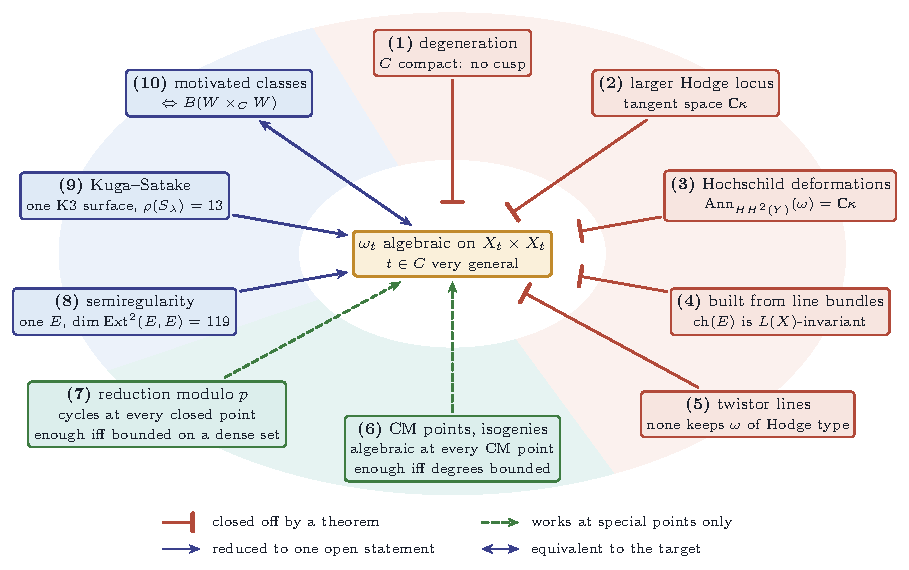
\includegraphics[width=0.96\textwidth]{fig_bypass}
\caption{\Cref{rem:bypassaudit}: the ten routes to the Mumford target that
avoid the Lefschetz standard conjecture. Clay, with a crossed dashed spoke: a
route closed off by a theorem of \Cref{ssec:mumfordrigid} or
\Cref{ssec:mumfordobject}. Grass: a route that works at special points only,
at the CM points or at the closed points of the reductions modulo $p$, and
suffices exactly when a degree bound holds (\Cref{cor:mumfordbounded},
\Cref{thm:modpdensity}). Indigo: a route reduced to one statement, of
the same kind as the target or equivalent to it.}
\label{fig:bypass}
\end{figure}

\subsection{Objects, reduction modulo $p$ and the motivic group}
\label{ssec:mumfordobject}

\Cref{thm:mumfordnumerical} reduces the semiregularity route to one object at
one CM point. We first derive what any object with the right Chern character
must satisfy, whether or not it is semiregular: no sequence of standard
operations produces it from line bundles; it extends along no first order
deformation of $D^{b}(Y)$ other than the direction of the curve; if it is
semiregular, it splits only into summands with no $\Ext^{2}$ between them;
and its self-extensions are large in every degree, with an odd part that the
Euler characteristic forces beyond what Hochschild cohomology supplies. We
then turn to reduction modulo $p$. By Li's proof of the Tate conjecture for
powers of abelian fourfolds over finite fields, the classes are represented
by cycles at every closed point of every reduction of the curve, and the
target is equivalent to a bound on those cycles on a Zariski dense set of
closed points. Finally, the motivic group of $X$ is one of four groups, and
the kinds of algebraic classes known on products of $X$ with other abelian
varieties generate no exceptional class. None of this constructs such an
object or proves the target.

\begin{lemma}[The contraction ranks are symmetric]\label{lem:rankduality}
Let $A$ be an abelian variety of dimension $g$ and $c\in H^{*}(A,\CC)$ a class
each of whose components has Hodge type $(p,p)$ for some $p$. For $k\ge0$ put
$r_{k}(c)=\dim\bigl(HT^{k}(A)\lrcorner\,c\bigr)$, with the action of
\Cref{setup:hh}. Then $r_{k}(c)=r_{g-k}(c)$ for $0\le k\le g$, and
$r_{k}(c)=0$ for $k>g$.
\end{lemma}

\begin{proof}
Write $H^{1,0}=H^{1,0}(A)$ and $A'=H^{0,1}(A)$, both of dimension $g$, so
that $H^{*}(A,\CC)=\bigwedge^{*}H^{1,0}\otimes\bigwedge^{*}A'$ and
$HT^{*}(A)=\bigwedge^{*}(A'\oplus T)$ with $T=(H^{1,0})^{\vee}$. Fix a
generator of $\bigwedge^{g}A'$ and let
$\star\colon\bigwedge^{q}A'\to\bigwedge^{g-q}A'^{\vee}$ send $\eta$ to
$\zeta\mapsto\eta\wedge\zeta$. Under $\Phi=\mathrm{id}\otimes\star$, wedging
with $z\in A'$ becomes, up to a sign fixed on each bigraded piece, contraction
with $z$ on the second factor, while $T$ still contracts the first. So $\Phi$
identifies the action of $HT^{*}(A)$ with the action of
$\bigwedge^{*}U^{\vee}$ by interior products on $\bigwedge^{*}U$, where
$U=H^{1,0}\oplus A'^{\vee}$ has dimension $2g$, up to signs that do not change
ranks. A class of type $(p,p)$ goes to
$\bigwedge^{p}H^{1,0}\otimes\bigwedge^{g-p}A'^{\vee}\subset\bigwedge^{g}U$,
so $\eta=\Phi(c)$ lies in the middle degree whatever the $p$ of its
components. Hence $r_{k}(c)$ is the rank of
$\bigwedge^{k}U^{\vee}\to\bigwedge^{g-k}U$, $x\mapsto\iota_{x}\eta$, which is
zero for $k>g$. Its transpose for the natural pairings is
$\bigwedge^{g-k}U^{\vee}\to\bigwedge^{k}U$, $y\mapsto\pm\iota_{y}\eta$,
because $\langle\iota_{x}\eta,y\rangle=\langle\eta,x\wedge y\rangle
=\pm\langle\iota_{y}\eta,x\rangle$. A map and its transpose have the same
rank.
\end{proof}

\begin{theorem}[The self-extensions of an object with an exceptional Chern
character]\label{thm:mumfordprofile}
Let $c\in C$ and $Y=X_{c}\times X_{c}$, and write
$e_{k}=\dim\Ext^{k}(E,E)$ for a perfect complex $E$ on $Y$.
\begin{enumerate}[label=\textup{(\roman*)},leftmargin=2.6em,itemsep=2pt]
\item For every $E$ and every $k$, $e_{k}\ge r_{k}(\ch E)$ and
  $e_{k}=e_{8-k}$.
\item For a rational exceptional class $\omega=\omega_{a}$ with
  $L_{0}(a)\ne0$: $r_{0}=r_{8}=1$, $r_{1}=r_{7}=16$ and $r_{2}=r_{6}=119$.
\item Let $\omega$ be a rational exceptional class and $\ch(E)=N\omega$
  with $N\ne0$. Then
  \[
    e_{1}+e_{3}=e_{0}+e_{2}+\tfrac12e_{4}
      +\sum_{j\ge1}(-1)^{j}e_{-j}.
  \]
  If $\Ext^{<0}(E,E)=0$, for instance if $E$ is a sheaf, then
  $\sum_{k\ \mathrm{odd}}e_{k}=\sum_{k\ \mathrm{even}}e_{k}$, and
  $e_{1}+e_{3}\ge120+\frac12e_{4}$ when $L_{0}(a)\ne0$.
\end{enumerate}
\end{theorem}

\begin{proof}
(i) The identity $\sigma_{E}\circ\operatorname{ev}_{E}=(\,\cdot\,)\lrcorner
\ch(E)$ of \Cref{setup:hh} holds in every degree, so the kernel of
$\operatorname{ev}_{E}$ on $HT^{k}(Y)$ lies in the annihilator of $\ch(E)$,
and the image of $HT^{k}(Y)$ in $\Ext^{k}(E,E)$ has dimension at least
$r_{k}(\ch E)$. Serre duality with the trivial canonical bundle gives
$e_{k}=e_{8-k}$.

(ii) $r_{0}=1$ because $\omega\ne0$, and $r_{2}=119$ is
\Cref{thm:mumfordrigid}(ii). If $w\in HT^{1}(Y)$ annihilates $\omega$, so does
$w'\wedge w$ for every $w'\in HT^{1}(Y)$, since the annihilator is a left
ideal; for $w\ne0$ these products span a space of dimension $15$, which cannot
lie in $\Ann_{HT^{2}}(\omega)=\CC\kappa$. So $r_{1}=16$, and
\Cref{lem:rankduality} gives $r_{8},r_{7},r_{6}$.

(iii) Since $\ch(E)$ has only a component in $H^{4}$, $\ch(E^{\vee})\ch(E)$
lies in $H^{8}(Y)$ and $\chi(E,E)=\int_{Y}\ch(E^{\vee})\ch(E)=0$, the Todd
class being trivial. By (i) and Serre duality, which also pairs
$\Ext^{-j}$ with $\Ext^{8+j}$,
\[
  0=\chi(E,E)=2(e_{0}-e_{1}+e_{2}-e_{3})+e_{4}
  +2\sum_{j\ge1}(-1)^{j}e_{-j},
\]
which is the displayed identity. With no negative extensions the odd and even
parts are equal, and $e_{0}\ge1$, $e_{2}\ge119$ by (i) and (ii) when
$L_{0}(a)\ne0$.
\end{proof}

\begin{proposition}[Divisor classes do not reach the exceptional classes]
\label{prop:mumforddivisor}
Let $t\in C$ and let $\omega$ be a rational exceptional class. Then $\omega_{t}$
is not in the $\QQ$-span of products of divisor classes of $X_{t}\times
X_{t}$: that span meets the rational Hodge classes of $H^{2}\otimes H^{2}$
exactly in the classes with $\alpha\in\QQ$. Consequently no perfect complex
whose Chern character lies in the subring generated by divisor classes, in
particular no bounded complex of direct sums of line bundles, has
$\ch(E)=N\omega$ with $N\ne0$. At a CM point $c$ the fourfold $X_{c}$ has eight
Hodge classes in $H^{4}$, of which the products of divisor classes span six.
\end{proposition}

\begin{proof}
At a point with Hodge group $G$, the divisor classes of $X_{t}\times X_{t}$ are
the three classes of \Cref{prop:mumfordproduct}(ii), all invariant under
$\Sp(V,\psi)$, and so are their products; the $\Sp(V,\psi)$-invariant part of
$H^{2}\otimes H^{2}$ is spanned by $\pi_{0}$ and $\pi_{12}+\pi_{13}+\pi_{23}$,
the classes with $a_{1}=a_{2}=a_{3}$. At a CM point the Hodge group is a
maximal torus of $G$ (proof of \Cref{thm:mumfordcm}), so the Hodge classes
are the monomials of weight zero. The proof of \Cref{prop:cmsource}(ii)
counts them: $16$ divisor classes $e^{(i)}_{w}e^{(j)}_{-w}$, $132$ Hodge
classes in degree four, of which the products of divisor classes span $100$,
and modulo that span
$\omega_{a}\equiv\frac12\bigl((a_{2}-a_{3})u_{12}+(a_{1}-a_{3})u_{13}
+(a_{1}-a_{2})u_{23}\bigr)$ with $u_{12},u_{13},u_{23}$ linearly independent.
So the span meets that of the four $\pi$ in exactly the classes with
$a_{1}=a_{2}=a_{3}$. For a rational class these
coordinates are the conjugates of $\alpha$, which by \Cref{lem:conjugates} are
equal only if $\alpha\in\QQ$. The Chern character of a complex in the subring
generated by divisor classes has its component in $H^{4}$ in the span of
products of two divisor classes, which excludes $N\omega$. For $X_{c}$ itself
the monomials of weight zero in $H^{4}$ are the six products
$e_{w}e_{-w}e_{w'}e_{-w'}$ over two opposite pairs, which are products of
divisor classes, and the two tetrahedron monomials.
\end{proof}

At a CM point the Hodge classes of $X_{c}$ in $H^{4}$ that are not products
of divisor classes are among the classes that the proof of
\Cref{thm:mumfordcm} pulls back along homomorphisms $X_{c}\times X_{c}\to
X_{c}$; they are algebraic by Markman's theorem \cite{Mar25a}. Li proves,
independently and more generally, that every Hodge class on every power of
every complex CM abelian fourfold is algebraic \cite[Theorem~1.3]{Li26}, which
gives \Cref{thm:mumfordcm} for every power $X_{c}^{n}$ and not only for the
square.

By \Cref{prop:mumforddivisor}, an object with $\ch(E)=N\omega$ cannot have
its Chern character in the subring generated by divisor classes, so it cannot
be assembled from line bundles alone. The next theorem shows that no sequence
of the standard operations of the derived category, applied to line bundles
on powers of $X_{t}$, gets any further.

\begin{theorem}[Objects generated by line bundles]\label{thm:lefschetzclosure}
Let $t\in C$, $X=X_{t}$, and let $L(X)\subseteq\Sp(V,\psi)$ be the Lefschetz
group of $X$, the centraliser of $\End^{0}(X)$ in $\Sp(V,\psi)$. Let
$\mathcal{A}$ be the class of abelian varieties isogenous to a power of $X$;
through an isogeny $X^{n}\to B$ the group $L(X)$ acts diagonally on
$H^{*}(B,\QQ)$, and the action does not depend on the isogeny. Let
$\mathcal{L}$ be the smallest class of objects of the categories
$D^{b}(B)$, $B\in\mathcal{A}$, that contains the line bundles and is closed
under shifts, cones, derived tensor products, derived duals, translations,
the functors $Lf^{*}$ and $Rf_{*}$ for homomorphisms $f$ between members of
$\mathcal{A}$, and the Fourier--Mukai functors $\Phi_{K}\colon D^{b}(B)\to
D^{b}(B')$ with kernel $K\in\mathcal{L}$ on $B\times B'$.
\begin{enumerate}[label=\textup{(\roman*)},leftmargin=2.6em,itemsep=2pt]
\item Every object of $\mathcal{L}$ has an $L(X)$-invariant Chern character.
\item $L(X)=\Sp(V,\psi)$ if $t$ is not a CM point, and $L(X)$ is a maximal
  torus of $\Sp(V,\psi)$ if it is. In both cases the $L(X)$-invariant classes
  on $X\times X$ form the subring generated by divisor classes, of dimensions
  $1,3,6,10,15,10,6,3,1$, respectively $1,16,100,304,454,304,100,16,1$, in
  the degrees $0,2,\dots,16$.
\item No rational exceptional class $\omega_{t}$ is $L(X)$-invariant. Hence
  for no object $E\in\mathcal{L}$ on $X\times X$ and no $N\ne0$ is
  $\ch(E)-N\omega_{t}$ invariant under $L(X)$; in particular
  $\ch(E)\ne N\omega_{t}$.
\item The $\Sp(V,\psi)$-module generated by $\pi_{12}-\pi_{13}$ is
  irreducible, of highest weight $2\varpi_{2}$ and dimension $308$, and it
  meets the span of the four $\pi$ in the plane of the classes with
  $a_{0}=0$ and $a_{1}+a_{2}+a_{3}=0$.
\end{enumerate}
\end{theorem}

\begin{proof}
(i) Two isogenies $X^{n}\to B$ differ by an element of $\End^{0}(X^{n})=
M_{n}(\End^{0}(X))$, which commutes with $L(X)$ acting diagonally, so the
action is well defined. For the same reason a homomorphism $f$ between members
of $\mathcal{A}$ is $L(X)$-equivariant on $H^{1}$, so $f^{*}$ is equivariant
on $H^{*}$, and so is $f_{*}$, which is $f^{*}$ conjugated by Poincar\'e
duality, since $L(X)\subseteq\SL(V)$ fixes the orientation classes.
Translations act trivially on cohomology. The Chern character is additive on
distinguished triangles and multiplicative on derived tensor products,
$\ch(E^{\vee})=\sum_{i}(-1)^{i}\ch_{i}(E)$, $\ch(Lf^{*}E)=f^{*}\ch(E)$, and
$\ch(Rf_{*}E)=f_{*}\ch(E)$ by the Grothendieck--Riemann--Roch theorem
\cite[Theorem~15.2]{Ful98}, the Todd class of an abelian variety being $1$;
and $\Phi_{K}=Rp_{2*}(p_{1}^{*}(\,\cdot\,)\otimes^{L}K)$. So the objects with
$L(X)$-invariant Chern character form a class with all the closure
properties, and it remains to see that it contains the line bundles, that is,
that $c_{1}(\mathcal{O}(D))$ is $L(X)$-invariant. Pulled back along an
isogeny, which is injective on rational cohomology, $c_{1}$ becomes a Hodge
class of degree two on some $X^{n}$, an element of the invariants of the
Hodge group in ${\textstyle\bigwedge^{2}}(V^{\vee}\otimes\QQ^{n})=
{\textstyle\bigwedge^{2}}V^{\vee}\otimes S^{2}\QQ^{n}\oplus S^{2}V^{\vee}
\otimes{\textstyle\bigwedge^{2}}\QQ^{n}$. If $t$ is not a CM point, the Hodge
group is $G$, whose invariants in ${\textstyle\bigwedge^{2}}V$ are the multiples of $\psi$
and in $S^{2}V$ are zero, since every summand of $S^{2}(V_{1}\otimes V_{2}
\otimes V_{3})$ contains a factor $S^{2}V_{i}$; so the Hodge classes of degree
two are $\Sp(V,\psi)$-invariant. If $t$ is a CM point, a monomial of degree two
in a weight basis has weight zero for the Hodge torus exactly when its two
weights are opposite, and then it has weight zero for $L(X)$, by the
description in (ii).

(ii) If $t$ is not a CM point, $\End^{0}(X)=\QQ$ and $L(X)=\Sp(V,\psi)$. At a
CM point $\End^{0}(X)\otimes\CC$ is the algebra of diagonal matrices in a
weight basis (proof of \Cref{thm:mumfordcm}), and $\psi$ pairs each weight
with its opposite only, so $L(X)_{\CC}$ is the torus of diagonal matrices
$\operatorname{diag}(\lambda_{w})$ with $\lambda_{w}\lambda_{-w}=1$, of rank
four. For $t$ not CM, the first fundamental theorem for $\Sp(V,\psi)$
\cite[Chapter~5]{GW09} shows that its invariants in
${\textstyle\bigwedge^{*}}(V\otimes\QQ^{2})$ are spanned by the products of
the three quadratic invariants, which are the divisor classes. Their
dimensions follow from the skew Cauchy formula
${\textstyle\bigwedge^{2m}}(V\otimes\QQ^{2})=\bigoplus_{\lambda}S_{\lambda}V
\otimes S_{\lambda'}\QQ^{2}$, over the partitions $\lambda=(2^{r},1^{s})$ of
$2m$ with at most two columns, and the rule that $S_{\lambda}V$ contains the
trivial representation of $\Sp(V,\psi)$, then once, exactly when both columns
of $\lambda$ have even length at most $8$ \cite{GW09}: the invariants of
degree $2m$ have dimension $\sum(s+1)$, over the even $r,s\ge0$ with
$2r+s=2m$ and $r+s\le8$, which is $1,3,6,10,15,10,6,3,1$ for
$m=0,\dots,8$. At a CM point the invariants are spanned by the
monomials of weight zero for $L(X)$; a set of weights $\pm e_{j}$ with sum
zero is a union of opposite pairs, so each such monomial is, up to sign, a
product of monomials of degree two and weight zero, which are divisor
classes. For each opposite pair $\{w,-w\}$ the four vectors
$e^{(1)}_{\pm w}$, $e^{(2)}_{\pm w}$ give one monomial of weight zero in
degree $0$, four in degree $2$ and one in degree $4$, so the numbers of these
monomials are the coefficients of $(1+4y+y^{2})^{4}$.

(iii) If $t$ is not a CM point, the $\Sp(V,\psi)$-invariant combinations of the
$\pi$ are those with $a_{1}=a_{2}=a_{3}$ (\Cref{prop:mumforddivisor}), and
the coefficients of $\omega_{t}$ are the distinct conjugates of $\alpha$
(\Cref{lem:conjugates}). At a CM point use the map $x\mapsto E_{x}$ of the
proof of \Cref{lem:oneexceptional}, which is $\Sp(V,\psi)$-equivariant: it
carries $\omega_{t}$ to an element $(r,\beta)$ of $\QQ\times F$ with
$\beta\notin\QQ$, acting on $U_{ij}$ by the conjugate $\sigma_{k}(\beta)$
(\Cref{prop:mumfordrm}(ii)), and $\omega_{t}$ is $L(X)$-invariant only if
$E_{\omega_{t}}$ preserves the weight spaces of $L(X)$ in ${\textstyle\bigwedge^{2}}V$. Take
weight vectors $v=x\otimes y\otimes z$ and $w=x\otimes y'\otimes z'$ of
weights $(1,1,1)$ and $(1,-1,-1)$ for the Hodge torus. They are not
opposite, so $v\wedge w$ spans a weight space of $L(X)$, every weight of
$L(X)$ on $V$ having multiplicity one. But
$v\wedge w=(x\cdot x)\otimes\bigl(y\cdot y'\otimes z\wedge z'+y\wedge y'
\otimes z\cdot z'\bigr)$ has nonzero components in $U_{12}$ and in $U_{13}$,
on which $E_{\omega_{t}}$ acts by $\sigma_{3}(\beta)\ne\sigma_{2}(\beta)$. So
the line is not preserved. The rest of (iii) follows from (i).

(iv) Write $H^{2}(X)=\QQ\theta\oplus P$, with $P$ the primitive part, the
irreducible $\Sp(V,\psi)$-module of highest weight $\varpi_{2}$ and dimension
$27$. Through the form ${\textstyle\bigwedge^{2}}\psi$ the four $\pi$ are
self-adjoint endomorphisms of $H^{2}(X)$, and $\pi_{12}-\pi_{13}$ kills
$\theta$ and is a trace-free self-adjoint endomorphism of $P$, an element of
$S^{2}P$ orthogonal to the invariant. Restricting
$S^{2}({\textstyle\bigwedge^{2}}V)=S_{(2,2)}V\oplus{\textstyle\bigwedge^{4}}V$
from $\GL(V)$ to $\Sp(V,\psi)$ gives, with dimensions $336=308+27+1$ and
$70=42+27+1$, the decomposition $S^{2}P=V(2\varpi_{2})\oplus V(\varpi_{4})
\oplus V(\varpi_{2})\oplus\QQ$. The element $\pi_{12}-\pi_{13}$ is
$G$-invariant. The summand $V(\varpi_{2})\cong P$ has no $G$-invariant, since
$({\textstyle\bigwedge^{2}}V)^{G}=\QQ\theta$, and neither has $V(\varpi_{4})$,
which lies in ${\textstyle\bigwedge^{4}}V$, whose $G$-invariants are the line
of $\theta^{2}$ (\Cref{prop:mumfordproduct}(i)), invariant under all of
$\Sp(V,\psi)$. So $\pi_{12}-\pi_{13}$ is a nonzero vector of the irreducible
module $V(2\varpi_{2})$, which it generates; its dimension is $308$ by Weyl's
dimension formula. The same argument puts every trace-free combination of
$\pi_{12},\pi_{13},\pi_{23}$ in $V(2\varpi_{2})$, while $\pi_{0}$ and
$\pi_{12}+\pi_{13}+\pi_{23}$ are $\Sp(V,\psi)$-invariant and independent
modulo it; so adding the four $\pi$ raises the dimension by two.
\end{proof}

\Cref{fig:hodgecount} compares the Hodge classes of $X_{t}\times X_{t}$ with
the subring generated by divisor classes, degree by degree.

\begin{figure}[htbp]
\centering
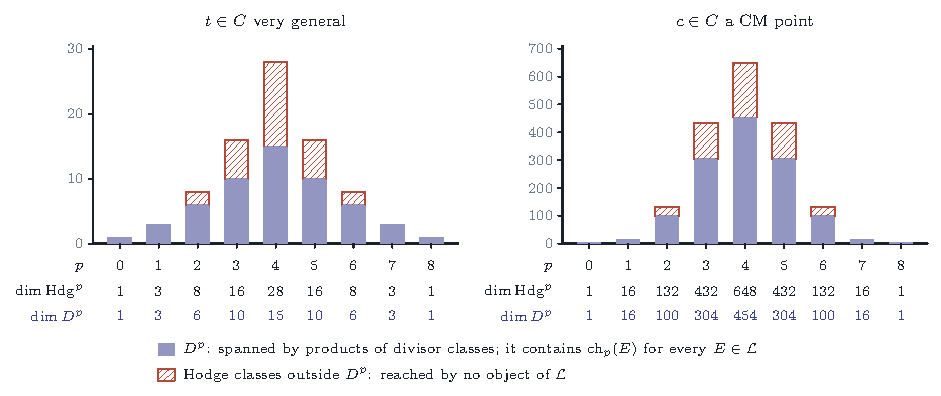
\includegraphics[width=\textwidth]{fig_hodgecount}
\caption{\Cref{thm:lefschetzclosure}(ii). The Hodge classes of
$X_{t}\times X_{t}$ degree by degree, against the subring $D^{p}$ generated
by divisor classes, which contains the Chern character of every object of
$\mathcal{L}$: at a very general point of the Mumford curve (left) and at a
CM point (right). The hatched classes, the exceptional ones among them, are
reached by no object of $\mathcal{L}$.}
\label{fig:hodgecount}
\end{figure}

\begin{remark}[Where a construction has to leave $\mathcal{L}$]
\label{rem:leavel}
\Cref{thm:lefschetzclosure} extends \Cref{prop:mumforddivisor} from sums of
line bundles to everything the standard operations make out of them, at every
point of the curve, including the CM points, where the exceptional classes
are algebraic. There the cycles that represent them are not Chern characters
of objects of $\mathcal{L}$, and neither are the two Hodge classes of $X_{c}$
in degree four that are not products of divisor classes. At a point that is
not CM, every Chern character of an object of $\mathcal{L}$ lies in the
isotypic component of the trivial representation of $\Sp(V,\psi)$, while by
\Cref{thm:lefschetzclosure}(iv) an object with $\ch(E)=N\omega$ must have a
nonzero component in the one of highest weight $2\varpi_{2}$. Every
construction of such an object therefore contains a step that does not commute with the Lefschetz group on
cohomology: passing to a direct summand, a subobject or a Jordan--H\"older
factor, choosing a point of a moduli space, or deforming from a member with
more endomorphisms. The last is what semiregularity does along the curve
(\Cref{thm:mumfordnumerical}).
\end{remark}

\begin{lemma}[The summands of a semiregular object]\label{lem:semiregsum}
Let $Z$ be a smooth projective variety and $E_{1},E_{2}$ perfect complexes on
$Z$. On $\Ext^{2}(E_{1}\oplus E_{2},E_{1}\oplus E_{2})=\bigoplus_{i,j}
\Ext^{2}(E_{j},E_{i})$ the semiregularity map is
$\sigma_{E_{1}\oplus E_{2}}(\zeta)=\sigma_{E_{1}}(\zeta_{11})
+\sigma_{E_{2}}(\zeta_{22})$. So $\sigma_{E_{1}\oplus E_{2}}$ is injective if
and only if $\sigma_{E_{1}}$ and $\sigma_{E_{2}}$ are injective, their images
meet only in zero, and $\Ext^{2}(E_{1},E_{2})=\Ext^{2}(E_{2},E_{1})=0$.
\end{lemma}

\begin{proof}
The Atiyah class is natural, so $\mathrm{At}(E_{1}\oplus E_{2})$ is the
diagonal sum of $\mathrm{At}(E_{1})$ and $\mathrm{At}(E_{2})$. In
$\sigma(\zeta)=\sum_{q}\frac1{q!}\operatorname{tr}(\zeta\circ\mathrm{At}^{q})$
of \Cref{thm:BF} the composite $\zeta\circ\mathrm{At}^{q}$ has diagonal blocks
$\zeta_{ii}\circ\mathrm{At}(E_{i})^{q}$, and the trace of a block matrix of
morphisms is the sum of the traces of its diagonal blocks. In particular the
off-diagonal blocks $\zeta_{12}$ and $\zeta_{21}$ lie in the kernel, so
injectivity forces them to vanish; on the diagonal blocks the map is
$(\zeta_{11},\zeta_{22})\mapsto\sigma_{E_{1}}(\zeta_{11})+\sigma_{E_{2}}
(\zeta_{22})$, which is injective exactly when both summands are injective
and their images meet only in zero.
\end{proof}

The condition on the images cannot be dropped, and the objects that show it
are the simplest ones: the structure sheaves of abelian subvarieties of half
dimension, each of which is semiregular on its own.

\begin{lemma}[Abelian subvarieties of half dimension are semiregular]
\label{lem:absemireg}
Let $A$ be an abelian variety of dimension $2n$ and $B\subseteq A$ an abelian
subvariety of dimension $n$. Then $\operatorname{ev}_{\cO_{B}}\colon
HT^{2}(A)\to\Ext^{2}(\cO_{B},\cO_{B})$ is surjective, its kernel is
$\Ann_{HT^{2}}([B])$, of dimension $6n^{2}-n$, and $\sigma_{\cO_{B}}$ is
injective.
\end{lemma}

\begin{proof}
The normal bundle of $B$ is trivial, so $\ch(\cO_{B})=[B]$ by the
Grothendieck--Riemann--Roch theorem for the embedding, and
$\Ext^{*}(\cO_{B},\cO_{B})\cong{\textstyle\bigwedge^{*}}\CC^{2n}$ (proof of
\Cref{cor:naturalsums}), so $\dim\Ext^{2}(\cO_{B},\cO_{B})=\binom{2n}{2}
=2n^{2}-n$, while $\dim HT^{2}(A)=2\binom{2n}{2}+4n^{2}=8n^{2}-2n$. Choose a
complementary abelian subvariety $B'$; the isogeny $B\times B'\to A$
identifies $H^{1}(A,\CC)$ with $H^{1}(B)\oplus H^{1}(B')$ compatibly with the
Hodge decompositions, identifies $HT^{2}(A)$ with $HT^{2}(B\times B')$
compatibly with contraction, and carries $[B]$ to a nonzero multiple of
$1\otimes[\mathrm{pt}_{B'}]$, where $[\mathrm{pt}_{B'}]$ spans
${\textstyle\bigwedge^{2n}}H^{1}(B')$. Write $T=T_{B}\oplus T_{B'}$ for the
tangent space and $H^{0,1}(A)=H^{0,1}(B)\oplus H^{0,1}(B')$. A class
$\zeta\in H^{0,2}(A)={\textstyle\bigwedge^{2}}H^{0,1}(A)$ has
$\zeta\cup[B]=\zeta_{BB}\otimes[\mathrm{pt}_{B'}]$, with $\zeta_{BB}$ its
component in ${\textstyle\bigwedge^{2}}H^{0,1}(B)$, because every factor from
$H^{0,1}(B')$ is killed by the top class of $B'$; so the annihilator in
$H^{0,2}$ has dimension $\binom{2n}{2}-\binom{n}{2}$. For $a\otimes v\in
H^{0,1}(A)\otimes T=H^{1}(T_{A})$ the contraction is $a\wedge(v\lrcorner[B])
=a_{B}\otimes(v_{B'}\lrcorner[\mathrm{pt}_{B'}])$, since $v_{B}$ kills
$[\mathrm{pt}_{B'}]$ and $a_{B'}\wedge(v_{B'}\lrcorner[\mathrm{pt}_{B'}])$
would have type $(n-1,n+1)$ on the $n$-fold $B'$; the map
$v\mapsto v_{B'}\lrcorner[\mathrm{pt}_{B'}]$ has rank $n$, as does
$a\mapsto a_{B}$, so the contraction has rank $n^{2}$ on the space
$H^{0,1}(A)\otimes T$ of dimension $4n^{2}$ and the annihilator there has
dimension $3n^{2}$. For $\vartheta\in{\textstyle\bigwedge^{2}}T$ only the
component in ${\textstyle\bigwedge^{2}}T_{B'}$ contracts $[\mathrm{pt}_{B'}]$
nontrivially, and injectively; so the annihilator in
${\textstyle\bigwedge^{2}}T$ has dimension $\binom{2n}{2}-\binom{n}{2}$.
Altogether $\dim\Ann_{HT^{2}}([B])=2\binom{2n}{2}-2\binom{n}{2}+3n^{2}
=6n^{2}-n$. By the square $\sigma_{E}\circ\operatorname{ev}_{E}=
(\,\cdot\,)\lrcorner\ch(E)$ of \Cref{setup:criterion} the kernel of
$\operatorname{ev}_{\cO_{B}}$ lies in $\Ann_{HT^{2}}([B])$, so
$\operatorname{ev}_{\cO_{B}}$ has rank at least $(8n^{2}-2n)-(6n^{2}-n)
=2n^{2}-n=\dim\Ext^{2}(\cO_{B},\cO_{B})$: it is surjective and its kernel is
the annihilator. If $\sigma_{\cO_{B}}(y)=0$, write $y=\operatorname{ev}(x)$;
then $x\lrcorner[B]=0$, so $x$ lies in the annihilator, which is the kernel,
and $y=0$.
\end{proof}

\begin{remark}[Sums of abelian subvarieties]\label{rem:absums}
Let $B_{1},\dots,B_{r}\subseteq A$ be abelian subvarieties of dimension
$n\ge3$, translated so that any two of them meet in finitely many points or
not at all, which generic translates achieve, and let $E=\bigoplus_{j}
\cO_{B_{j}}[k_{j}]$. The sheaves $\mathcal{E}xt^{q}(\cO_{B_{i}},\cO_{B_{j}})$
for $i\ne j$ are supported on $B_{i}\cap B_{j}$ and vanish for $q\ne n$,
by the Koszul resolution of $\cO_{B_{i}}$ restricted to $B_{j}$, so
$\Ext^{2}(\cO_{B_{i}}[k_{i}],\cO_{B_{j}}[k_{j}])=H^{2+k_{j}-k_{i}-n}
(B_{i}\cap B_{j},\mathcal{E}xt^{n})$ vanishes when all $k_{j}$ are equal and
$n\ge3$, and when $|k_{i}-k_{j}|\le1$ and $n\ge4$; and each
$\sigma_{\cO_{B_{j}}}$ is injective by \Cref{lem:absemireg}. In these cases
every hypothesis of \Cref{lem:semiregsum}, applied to one summand and the
sum of the others, holds except the one on the images. Now let $v\in HT^{2}(A)$
satisfy $v\lrcorner\ch(E)=\sum_{j}(-1)^{k_{j}}v\lrcorner[B_{j}]=0$ with
$v\lrcorner[B_{1}]\ne0$. Then $\zeta=\bigoplus_{j}\operatorname{ev}_{\cO_{B_{j}}}(v)$
is nonzero, because $v$ is not in the annihilator of $[B_{1}]$, and
$\sigma_{E}(\zeta)=\sum_{j}(-1)^{k_{j}}v\lrcorner[B_{j}]=0$: the images of
the $\sigma_{\cO_{B_{j}}}$ meet, and $E$ is not semiregular. This is exactly
the situation at a member of a Weil family on which a Weil class is a
combination of classes of abelian subvarieties of dimension $n$, as on a
product of elliptic curves: a tangent direction $v$ of the family keeps
$\ch(E)$ of Hodge type but moves any $[B_{j}]$ outside
$\QQ\theta^{n}\oplus\HW(A)$, and \Cref{cor:naturalsums} excludes such sums
for this reason. The sum is obstructed although its summands are not.
\end{remark}

\begin{corollary}[Hochschild deformations and direct summands]
\label{cor:mumfordsplit}
Let $c\in C$, $Y=X_{c}\times X_{c}$, $\omega=\omega_{a}$ a rational
exceptional class with $L_{0}(a)\ne0$, and $E$ a perfect complex on $Y$ with
$\ch(E)=N\omega$, $N\ne0$.
\begin{enumerate}[label=\textup{(\roman*)},leftmargin=2.6em,itemsep=2pt]
\item $E$ extends to the first order deformation of $D^{b}(Y)$ given by
  $x\in HH^{2}(Y)=HT^{2}(Y)$ only if $x\in\CC\kappa$. No $B$-field, no
  Poisson bivector and no commutative deformation off the curve carries it.
\item If $\sigma_{E}$ is injective and $E=E_{1}\oplus E_{2}$ with both
  summands nonzero, then $\Ext^{2}(E_{1},E_{2})=\Ext^{2}(E_{2},E_{1})=0$, each
  $\sigma_{E_{i}}$ is injective, each $E_{i}$ extends to first order along the
  curve, and $\kappa\lrcorner\ch(E_{i})=0$. If moreover
  $\dim\Ext^{2}(E,E)=119$, then $\dim\Ext^{2}(E_{i},E_{i})=
  120-\dim\Ann_{HT^{2}}(\ch E_{i})$, and
  \[
    \Ann_{HT^{2}}(\ch E_{1})+\Ann_{HT^{2}}(\ch E_{2})=HT^{2}(Y),\qquad
    \Ann_{HT^{2}}(\ch E_{1})\cap\Ann_{HT^{2}}(\ch E_{2})=\CC\kappa .
  \]
\end{enumerate}
\end{corollary}

\begin{proof}
(i) The kernel of $\operatorname{ev}_{E}$ on $HH^{2}(Y)$ is the space of
deformations of $D^{b}(Y)$ along which $E$ deforms to first order
\cite{Tod09}, \cite[Section~8.3]{Mar25a}. If $\operatorname{ev}_{E}(x)=0$ then
$N\,x\lrcorner\,\omega=\sigma_{E}(\operatorname{ev}_{E}(x))=0$, so
$x\in\CC\kappa$ by \Cref{thm:mumfordrigid}(ii). The three kinds of
deformation named are the three summands of $HT^{2}(Y)$.

(ii) The first two assertions are \Cref{lem:semiregsum}. By
\Cref{thm:mumfordnumerical}(ii), $\operatorname{ev}_{E}(\kappa)=0$, and
$\operatorname{ev}_{E}$ is the diagonal sum of $\operatorname{ev}_{E_{1}}$
and $\operatorname{ev}_{E_{2}}$, so each vanishes at $\kappa$; then
$\kappa\lrcorner\ch(E_{i})=\sigma_{E_{i}}(\operatorname{ev}_{E_{i}}(\kappa))
=0$. Put $e(x)=120-\dim\Ann_{HT^{2}}(x)$, the rank of contraction into $x$.
It is subadditive in $x$, and by \Cref{thm:mumfordprofile}(i)
$\dim\Ext^{2}(E_{i},E_{i})\ge e(\ch E_{i})$. The cross terms vanish, so
\[
  119=\dim\Ext^{2}(E,E)=\sum_{i}\dim\Ext^{2}(E_{i},E_{i})
  \ge e(\ch E_{1})+e(\ch E_{2})\ge e(N\omega)=119,
\]
and every inequality is an equality. Hence
$\dim\Ann(\ch E_{1})+\dim\Ann(\ch E_{2})=121$. The intersection of the two
annihilators lies in $\Ann(N\omega)=\CC\kappa$ and contains $\kappa$, so it is
$\CC\kappa$, and the sum has dimension $120$.
\end{proof}

Part (ii) plays for the Mumford classes the role of \Cref{thm:nosum}: a
semiregular object attaining the bound either does not split, or splits into
two pieces whose annihilators fill $HT^{2}(Y)$ and meet only in the direction
of the curve. The two annihilators are the analogue of the two branches $P$
and $Q$ of \Cref{rem:twobranches}.

\begin{proposition}[Tate classes at every closed point of every reduction]
\label{prop:modp}
There are a finitely generated subring $R\subset\CC$, a model $W_{R}\to
C_{R}$ of $W\to C$ over $R$, with $C_{R}$ smooth and projective over $R$ with
geometrically connected fibres and $W_{R}$ an abelian scheme, projective over
$C_{R}$, and a finite surjective morphism $C'_{R}\to C_{R}$ from a second curve of the same
kind, with the following properties. Put $Y'=(W_{R}\times_{C_{R}}W_{R})
\times_{C_{R}}C'_{R}$, with projection $\pi'\colon Y'\to C'_{R}$, and let
$\omega$ be a rational exceptional class. For every prime $\ell$ there is a
global section $\omega_{\ell}$ of the lisse sheaf
$R^{4}\pi'_{*}\QQ_{\ell}(2)$ on $C'_{R}[1/\ell]$ whose restriction to
$C'_{R}\otimes_{R}\CC$ is the pull-back of $\omega\otimes1$; write
$\omega_{\ell}(\bar{x})$ for its value at a geometric point over a point $x$.
\begin{enumerate}[label=\textup{(\roman*)},leftmargin=2.6em,itemsep=2pt]
\item At a closed point $x$ of $C'_{R}[1/\ell]$ the residue field
  $\kappa(x)$ is finite, $Y'_{x}$ is the square of an abelian fourfold over
  it, and $\omega_{\ell}(\bar{x})$ is fixed by $\Gal(\bar{\kappa}/\kappa(x))$.
\item At such a point $\omega_{\ell}(\bar{x})$ is a $\QQ_{\ell}$-linear
  combination of classes of algebraic cycles of codimension two on $Y'_{x}$,
  defined over $\kappa(x)$.
\item Let $s$ be a closed point of $\Spec R[1/\ell]$ and $\eta_{s}$ the generic
  point of the reduction $C'_{s}$. Then $\omega_{\ell}(\bar\eta_{s})$ is fixed
  by the Galois group of the function field $\kappa(\eta_{s})$, and it is not
  a $\QQ_{\ell}$-linear combination of products of divisor classes of
  $Y'_{\bar\eta_{s}}$.
\end{enumerate}
Every closed point $x$ of a reduction $C_{s}$ of $C$ is the image of a closed
point $x'$ of $C'_{s}$, and $Y'_{x'}=Y_{x}\otimes_{\kappa(x)}\kappa(x')$; so
(i) and (ii) hold at every closed point of every reduction of $C$, after a
finite extension of its residue field.
\end{proposition}

\begin{proof}
\emph{The models.} The family $W\to C$ is defined over a subfield
$k_{1}\subset\CC$ finitely generated over $\QQ$, say as $W_{1}\to C_{1}$. Let
$K_{1}$ be the function field of $C_{1}$ and fix an embedding over $k_{1}$ of
an algebraic closure $\bar{K}_{1}$ into $\CC$; it sends the geometric generic
point of $C_{1}$ to a point $t\in C$, and $Y_{t}=X_{t}\times X_{t}$ is the base
change of $Y_{\bar{K}_{1}}$. The class $\omega_{t}$ is a Hodge class on an
abelian variety, hence absolutely Hodge, so it comes from an absolutely Hodge
class of $Y_{\bar{K}_{1}}$, and $\Gal(\bar{K}_{1}/K_{1})$ acts on these
through a finite quotient \cite[Theorem~2.11 and Proposition~2.9]{Del82}. Let
$K'\subset\bar{K}_{1}$ be a finite extension of $K_{1}$ on which the action is
trivial, $k'$ the algebraic closure of $k_{1}$ in $K'$, and $C'$ the smooth
projective curve over $k'$ with function field $K'$; it is geometrically
connected over $k'$ and maps finitely onto $C_{1}\otimes_{k_{1}}k'$.
Spreading out $W_{1}\to C_{1}$, $C'$ and this map over a finitely generated
subring of $k'$, and inverting one element of it, gives a normal $R$ and
models with the stated properties.

\emph{The section.} By smooth and proper base change
$R^{4}\pi'_{*}\QQ_{\ell}(2)$ is lisse on $C'_{R}[1/\ell]$. Its stalk at the
geometric generic point $\Spec\bar{K}_{1}$ is $H^{4}(Y_{\bar{K}_{1}},
\QQ_{\ell}(2))=H^{4}(Y_{t},\QQ)\otimes\QQ_{\ell}$, and $\omega_{t}\otimes1$
is the $\ell$-adic component of an absolutely Hodge class, so it is fixed by
$\Gal(\bar{K}_{1}/K')$. The scheme $C'_{R}[1/\ell]$ is normal and integral
with function field $K'$, so $\Gal(\bar{K}_{1}/K')$ maps onto its fundamental
group \cite[Tag~0BQI]{Stacks}, and the vector extends to a global section
$\omega_{\ell}$. On the connected curve $C'_{R}\otimes_{R}\CC$ it agrees with
the pull-back of $\omega\otimes1$, the two being global sections of the same
local system that agree at a point over $t$.

(i) and (ii). A scheme of finite type over $\ZZ$ has finite residue fields at
its closed points. A global section of a lisse sheaf is fixed by the
fundamental group of every point, which is (i); and (ii) is Li's theorem
\cite[Theorem~1.1]{Li26}, with $n=r=2$, for the abelian fourfold that is the
fibre of $W_{R}$ at the image of $x$, base changed to $\kappa(x)$.

(iii) The first assertion holds for the same reason as (i). For the second,
let $\bar\eta$ be a geometric generic point of $C'_{R}$ and $\bar{s}$ a
geometric point over $s$. The morphism $C'_{R}\to\Spec R$ is flat and proper
with geometrically connected and geometrically reduced fibres, so the
specialisation map $\pi_{1}(C'_{\bar\eta})\to\pi_{1}(C'_{\bar{s}})$ is
surjective \cite[Tag~0C0P]{Stacks}, and it is compatible with the actions of
the two groups on the first cohomology of the fibres of $W_{R}$, identified by
cospecialisation. The image of $\pi_{1}(C'_{\bar\eta})$ contains that of
$\pi_{1}(C'_{\CC})$, the closure of the image of the topological fundamental
group of a finite cover of $C$, whose Zariski closure contains
$G_{\QQ_{\ell}}$ because the connected monodromy group of $W\to C$ is $G$
(proof of \Cref{cor:mumfordlefschetz}). So the Zariski closure of the
monodromy of $W_{R}$ over $C'_{\bar{s}}$ contains $G_{\QQ_{\ell}}$. A divisor
class of $Y'_{\bar\eta_{s}}$ is defined over a finite extension of
$\kappa(\eta_{s})$, so it is fixed by an open subgroup of the Galois group,
whose image in $\pi_{1}(C'_{s})$ is open \cite[Tag~0BQI]{Stacks} and meets
$\pi_{1}(C'_{\bar{s}})$ in an open subgroup; the Zariski closure of the image
of an open subgroup has the same identity component, so the class is
$G_{\QQ_{\ell}}$-invariant. The $G$-invariants of ${\textstyle\bigwedge^{2}}(V\oplus V)$ are the
three divisor classes of \Cref{prop:mumfordproduct}(ii), which are
$\Sp(V,\psi)$-invariant, so every product of divisor classes of
$Y'_{\bar\eta_{s}}$ is $\Sp(V,\psi)$-invariant. The class
$\omega_{\ell}(\bar\eta_{s})$ corresponds to $\omega\otimes1$, whose
coefficients $a_{1},a_{2},a_{3}$ are the distinct conjugates of $\alpha$
(\Cref{lem:conjugates}), and the $\Sp(V,\psi)$-invariant classes among the
$\omega_{a}$ are those with $a_{1}=a_{2}=a_{3}$ (\Cref{prop:mumforddivisor}).
The last sentence of the statement holds because $C'_{R}\to C_{R}$ is finite
and surjective.
\end{proof}

At the generic point of each reduction the class is therefore a Tate class
over a global function field that is not a combination of products of divisor
classes, exactly as over $\CC$, while at every closed point it is a
combination of classes of cycles. The next theorem shows that a bound on those
cycles is all that is missing, with no passage through $p$-adic Hodge theory.

\begin{theorem}[The Mumford target is a degree bound in positive
characteristic]\label{thm:modpdensity}
Keep \Cref{prop:modp}, fix a prime $\ell$ and a relatively ample line bundle
on $Y'\to C'_{R}$, and for a finite set $\Phi$ of tuples of Hilbert
polynomials say that $\omega$ is \emph{$\Phi$-represented} at a point $x$ of
$C'_{R}[1/\ell]$ if $\omega_{\ell}(\bar{x})=\sum_{i}q_{i}\operatorname{cl}(Z_{i})$
for some $q_{i}\in\QQ_{\ell}$ and closed subschemes $Z_{i}\subset Y'_{\bar{x}}$
of pure codimension two whose Hilbert polynomials form a tuple in $\Phi$. The
following are equivalent.
\begin{enumerate}[label=\textup{(\alph*)},leftmargin=2.6em,itemsep=2pt]
\item $\omega_{t}$ is algebraic for every $t\in C$.
\item For some finite $\Phi$, the closed points of $C'_{R}[1/\ell]$ at which
  $\omega$ is $\Phi$-represented are Zariski dense in $C'_{R}$.
\item For some finite $\Phi$ and some Zariski dense set $S$ of closed points of
  $\Spec R[1/\ell]$, the class $\omega$ is $\Phi$-represented at infinitely
  many closed points of $C'_{s}$ for every $s\in S$.
\end{enumerate}
For a single closed point $s$ of $\Spec R[1/\ell]$, the class $\omega$ is
$\Phi$-represented at infinitely many closed points of $C'_{s}$, for some
finite $\Phi$, if and only if $\omega_{\ell}(\bar\eta_{s})$ is a
$\QQ_{\ell}$-linear combination of classes of algebraic cycles on
$Y'_{\bar\eta_{s}}$.
\end{theorem}

\begin{proof}
One standard property of the $\ell$-adic cycle class is used beyond those over
a field: if $\mathcal{O}$ is a discrete valuation ring in which $\ell$ is
invertible, $\mathcal{Y}\to\Spec\mathcal{O}$ is smooth and projective, and
$\mathcal{Z}\subset\mathcal{Y}$ is a closed subscheme flat over $\mathcal{O}$,
then the specialisation isomorphism of $\ell$-adic cohomology carries the
cycle class of the geometric generic fibre of $\mathcal{Z}$ to that of its
geometric special fibre \cite[Cycle]{SGA4h}. The specialisation isomorphism
also carries the values of a global section of a lisse sheaf to each other,
by its construction.

\emph{Step 1: the represented loci are closed.} For a tuple
$\underline{P}=(P_{1},\dots,P_{m})$ let $\cH_{\underline{P}}$ be the fibre
product over $C'_{R}[1/\ell]$ of the relative Hilbert schemes
$\Hilb^{P_{i}}(Y'/C'_{R}[1/\ell])$. It is projective over $C'_{R}[1/\ell]$
\cite{Gro61}, so it has finitely many connected components. On a component
$T$, with universal subschemes $\mathcal{Z}_{i}$, put $A(h)=\{q\in
\QQ_{\ell}^{m}:\sum_{i}q_{i}\operatorname{cl}(\mathcal{Z}_{i,\bar{h}})
=\omega_{\ell}(\bar{h})\}$ for $h\in T$. If $h'$ is a specialisation of $h$,
there is a discrete valuation ring mapping to $T$ with generic point to $h$ and
closed point to $h'$ \cite[Tag~054F]{Stacks}, and the property above, applied
to the pull-backs of $Y'$ and of the $\mathcal{Z}_{i}$, gives $A(h)=A(h')$.
Any two points of the connected noetherian scheme $T$ are joined by a chain of
specialisations and generisations, through the generic points of its
irreducible components, so $A$ is constant on $T$, say $A_{T}$. Let
$\Sigma_{\underline{P}}$ be the union of the images in $C'_{R}[1/\ell]$ of the
components $T$ with $A_{T}\ne\emptyset$. It is closed, as a finite union of
images of proper morphisms, and it is the set of points at which $\omega$ is
$\{\underline{P}\}$-represented: at a point $x$ of the image of such a $T$, a
closed point of the fibre of $T$ over $x$ has residue field finite over
$\kappa(x)$ and gives subschemes of $Y'_{\bar{x}}$. Put
$\Sigma_{\Phi}=\bigcup_{\underline{P}\in\Phi}\Sigma_{\underline{P}}$.

\emph{Step 2: (b) implies (a).} $\Sigma_{\Phi}$ is closed and contains a dense
set, so it is $C'_{R}[1/\ell]$ and contains the generic point $\xi$ of
$C'_{R}$, whose residue field is $K'$. So $\omega_{t}\otimes1=
\omega_{\ell}(\bar\xi)=\sum_{i}q_{i}\operatorname{cl}(Z_{i})$ with
$q\in\QQ_{\ell}^{m}$ and subschemes $Z_{i}$ of $Y_{\bar{K}_{1}}$, and so of
$Y_{t}$. The cycle class maps are compatible with the comparison isomorphism
$H^{4}(Y_{t},\QQ)\otimes\QQ_{\ell}\cong H^{4}(Y_{t},\QQ_{\ell})$
\cite[Section~1 and Example~2.1(a)]{Del82}, so the linear system
$\omega_{t}=\sum_{i}q_{i}[Z_{i}]$, which has rational coefficients, is
solvable over $\QQ_{\ell}$, hence over $\QQ$, and $\omega_{t}$ is algebraic.
The $Z_{i}$ are defined over a finite extension of $K'$, so they spread out to
subschemes, flat over a nonempty open subset \cite[Tag~052A]{Stacks}, of the
pull-back of $W\times_{C}W$ to a finite cover of $C$, and by the local
constancy of the cycle class used in the proof of \Cref{thm:closedlocus},
$\omega$ is algebraic at every point of a nonempty Zariski open subset of $C$,
which is uncountable. \Cref{cor:mumfordequiv} gives (a).

\emph{Step 3: (c) implies (b).} Let $D$ be the set of closed points at which
$\omega$ is $\Phi$-represented and $\bar{D}$ its closure. For $s\in S$ the set
$D\cap C'_{s}$ is infinite, so its closure is the irreducible curve $C'_{s}$,
and $C'_{s}\subseteq\bar{D}$. The points $u$ of $\Spec R[1/\ell]$ over which
the fibre of $\bar{D}$ has dimension at least one form a closed set, by the
upper semicontinuity of the dimension of the fibres of a proper morphism
\cite[Tag~0D4I]{Stacks}; it contains the dense set $S$, so it contains the
generic point. The generic fibre of $\bar{D}$ is then a closed subset of
dimension one of the irreducible curve $C'_{R}\otimes_{R}k'$, so it contains
$\xi$, and $\bar{D}=C'_{R}[1/\ell]$.

\emph{Step 4: (a) implies (c).} By (a) and Step 1, applied over $\bar{K}_{1}$
with the Betti class in place of the $\ell$-adic one, $\omega_{t}$ is the
class of a rational combination of subschemes of $Y_{\bar{K}_{1}}$, defined
over a finite extension $L$ of $K'$. Enlarge $R$ to a finitely generated
subring of the algebraic closure of $k'$ in $L$, let $C''_{R}\to C'_{R}$ be the
normalisation in $L$, and spread the subschemes out over $C''_{R}$; by generic
flatness \cite[Tag~052A]{Stacks} they are flat over a dense open subset $U$ of
$C''_{R}[1/\ell]$, with constant Hilbert polynomials. By Step 1 applied on $U$,
$\omega$ is represented by their fibres at every point of $U$. The image of $U$
in $C'_{R}[1/\ell]$ contains a dense open subset $U'$, every closed point of
$U'$ is the image of a closed point of $U$, and $U'$ meets $C'_{s}$ in a
nonempty open, hence infinite, subset for every $s$ in a dense open subset of
$\Spec R[1/\ell]$.

\emph{The single reduction.} If $\omega$ is $\Phi$-represented at infinitely
many closed points of $C'_{s}$, then $\Sigma_{\Phi}\cap C'_{s}$ is closed and
infinite, so it is $C'_{s}$ and contains $\eta_{s}$. Conversely, cycles at
$\bar\eta_{s}$ are defined over a finite extension of $\kappa(\eta_{s})$, and
spreading them out as in Step 4 over a finite cover of $C'_{s}$ represents
$\omega$, with fixed Hilbert polynomials, at every closed point of a nonempty
open subset of $C'_{s}$.
\end{proof}

\begin{remark}[What is left in positive characteristic]\label{rem:modpremains}
By \Cref{prop:modp}(ii) the class is represented at every closed point of
$C'_{R}[1/\ell]$, so \Cref{thm:modpdensity} turns the Mumford target into a
statement of uniformity alone: the Hilbert data of some representation must
stay in one finite set on a Zariski dense set of closed points, for instance
at infinitely many closed points of infinitely many reductions. The passage
to characteristic zero is then done by the specialisation of cycle classes
along $C'_{R}$, and neither the $p$-adic variational Hodge conjecture nor a
lifting of cycles is needed. Li's theorem gives no bound: where its proof
carries cycles into a prescribed isogeny class, it does so by an isogeny whose
degree it does not control \cite[proof of Theorem~1.2, Step~3]{Li26}.

Nor do the natural representatives at the supersingular points supply the
bound. At a closed point $x$ whose fibre is supersingular, the Frobenius
eigenvalues on $H^{2}(Y'_{\bar{x}},\QQ_{\ell}(1))$ are roots of unity, so by
Tate's theorem \cite{Tat66} this space is spanned by divisor classes, and
$\omega_{\ell}(\bar{x})\in{\textstyle\bigwedge^{4}}H^{1}$ is a combination of
products of two of them. But for a closed point $s$ of $\Spec R[1/\ell]$ and
a finite set of Hilbert polynomials, only finitely many closed points of
$C'_{s}$ carry such a combination $\sum_{i}q_{i}\operatorname{cl}(D_{i})
\operatorname{cl}(D'_{i})$ with effective divisors $D_{i},D'_{i}$ whose
Hilbert polynomials lie in that set: otherwise Step~1 of the proof of
\Cref{thm:modpdensity}, run on relative Hilbert schemes of divisors, would
give one at $\bar\eta_{s}$, against \Cref{prop:modp}(iii). This holds whether
or not the supersingular points are dense. They are dense in $C'_{R}$ when $R$
has dimension one. Indeed, for every prime $p\ge5$ not dividing the
discriminants of $F$ and $D$, which is all but finitely many, the
supersingular points of the reduction at a prime over $p$ of Kisin's integral
model of the Shimura curve, with hyperspecial level at $p$, are its whole
Newton jumping locus and number $(p^{r}-1)(g-1)$ on each component of genus
$g$, $r$ being the local degree of $F$ \cite[Theorem~1.2 and
Corollary~5.17]{SZ11}. For all but finitely many $s$ the curve $C'_{s}$ maps
finitely onto such a component, of genus at least two, so it has at least
$p-1$ supersingular points, while a closed subset of $C'_{R}$ of dimension one
meets all but finitely many of the $C'_{s}$ in boundedly many points.

Within one reduction the bound is equivalent to the class being algebraic at
the generic point of $C'_{s}$ (\Cref{thm:modpdensity}), a Tate class over a
global function field that is not a combination of products of divisor
classes (\Cref{prop:modp}(iii)). This is the codimension two case of the
variational Tate conjecture along $C'_{s}$, which Morrow proves for divisors
in its crystalline form \cite{Mor19}. From one reduction alone, the way back
to characteristic zero would be the $p$-adic variational Hodge conjecture for
$W\times_{C}W$ over the Witt vectors of $\kappa(s)$, with rational rather than
$\ell$-adic coefficients and with the crystalline class of the cycle matching
the de Rham class of $\omega$. Bloch, Esnault and Kerz lift such a class in
$K_{0}\otimes\QQ$ of the special fibre to the formal completion for $p>15$,
the dimension being nine, and the algebraisation of the formal class is the
remaining step of their programme \cite[Theorem~1.3]{BEK14}. The route
therefore runs through the uniform bound or through this conjecture.
\end{remark}

Five of the routes of \Cref{rem:bypassaudit} survive the rigidity theorems:
\emph{specialisation}, \emph{reduction modulo $p$}, \emph{semiregularity},
\emph{Kuga--Satake} and \emph{motivated classes}. The next corollary shows
that they are not five separate obligations.

\begin{corollary}[The five routes reduce to one statement]\label{cor:mumfordone}
Let $W\to C$ be as in \Cref{cor:mumfordlefschetz}, let $\omega$ be a rational
exceptional class, and let the \emph{Mumford target} be the first case of
\textup{(F2)}: the Hodge conjecture for $X_{t}\times X_{t}$ for every $t\in C$.
\begin{enumerate}[label=\textup{(\roman*)},leftmargin=2.6em,itemsep=2pt]
\item Each of the following is equivalent to the Mumford target: $\omega_{t}$ is
  algebraic for uncountably many $t\in C$; $B(W\times_{C}W)$ holds for
  $L_{W\times_{C}W}$; $\omega$ is represented with Hilbert data in one finite
  set at infinitely many points of $C$, for instance at infinitely many CM
  points; $\omega$ is represented with Hilbert data in one finite set on a
  Zariski dense set of closed points of the arithmetic model of
  \Cref{thm:modpdensity}.
\item Each of the following implies the Mumford target: a perfect complex $E$
  at one point of $C$ with $\ch(E)=N\omega$, $N\ne0$, no other component, and
  $\dim\Ext^{2}(E,E)=119$; the algebraicity, for uncountably many $t$, of the
  Kuga--Satake class of the surface $S_{\lambda}$ of \Cref{thm:mumfordks}
  attached to $X_{t}$; a rational map as in \Cref{prop:hksquare}(iv), under
  its hypotheses, from $X_{t}\times X_{t}$ for uncountably many $t$.
\item There is a countable set $\Sigma_{0}\subset C$ containing the CM points
  such that the Mumford target holds as soon as the Hodge conjecture holds for
  $X_{c}\times X_{c}$ at one point $c\notin\Sigma_{0}$.
\end{enumerate}
\end{corollary}

\begin{proof}
(i) The first two are \Cref{cor:mumfordequiv}, with \Cref{lem:oneexceptional}
for one class in place of two, the third is \Cref{cor:mumfordbounded} and the
fourth is \Cref{thm:modpdensity}. (ii) The first is
\Cref{thm:mumfordnumerical}(iii). The second and the third give the Hodge
conjecture for $X_{t}\times X_{t}$ at each of the uncountably many points, by
\Cref{thm:mumfordks}(ii) and \Cref{prop:hksquare}(iv), and then (i) applies.
(iii) In the proof of \Cref{cor:mumfordbounded} the set of points at which
$\omega$ is algebraic is the union of the countably many closed sets
$\Sigma_{\underline{P},\underline{q}}$, each finite or equal to $C$. Let
$\Sigma_{0}$ be the union of the finite ones and of the CM points. If
$\omega_{c}$ is algebraic at a point $c\notin\Sigma_{0}$, then $c$ lies in
some $\Sigma_{\underline{P},\underline{q}}$ that is not finite, which is $C$,
and (i) applies.
\end{proof}

\begin{remark}[Which routes are needed]\label{rem:mumfordneeded}
Of the five routes, specialisation, reduction modulo $p$ and motivated
classes are the Mumford target itself in three other forms, by
\Cref{cor:mumfordone}(i) and, for the motivated classes,
\Cref{cor:mumfordequiv}; semiregularity and Kuga--Satake are stronger inputs
that imply it. So any one route suffices. Each of the three
forms is the whole of the problem, a bound on Hilbert data or a case of
\textup{(L)} that is equivalent to the target, and the two stronger inputs
ask for an object and for a cycle.
\end{remark}

The target can also be read at a single member, through the motivic group of
$X$ rather than through cycles on the family; it then becomes the question of
which of four groups this is.

\begin{proposition}[Four possible motivic groups]\label{prop:mumfordmotivic}
In \Cref{setup:mumford}, let $M$ be the group of the Tannakian category of
homological motives generated by $h(X)$, with the Betti realisation as fibre
functor, let $M^{1}=M\cap\Sp(V,\psi)$, and let $N$ be the normaliser of $G$ in
$\Sp(V,\psi)$. Over $\bar{\QQ}$ identify $V_{1}$, $V_{2}$ and $V_{3}$ with one
plane, carrying $\epsilon_{1}$, $\epsilon_{2}$, $\epsilon_{3}$ to one form, and
let $\zeta\in\Sp(V,\psi)(\bar{\QQ})$ be the cyclic permutation
$v_{1}\otimes v_{2}\otimes v_{3}\mapsto v_{3}\otimes v_{1}\otimes v_{2}$ of
the three factors. It normalises $G$, and other identifications change it by
an element of $G(\bar{\QQ})$; so it acts through $V$ on the Hodge classes of
every power of $X$, independently of the choice.
\begin{enumerate}[label=\textup{(\roman*)},leftmargin=2.6em,itemsep=2pt]
\item $N/G$ is a form of the symmetric group $S_{3}$,
  $M=\mathbb{G}_{m}\cdot M^{1}$, and $M^{1}$ is one of $G$, $G\cdot A_{3}$,
  $N$ and $\Sp(V,\psi)$, where $G\cdot A_{3}$ is the inverse image in $N$ of
  the subgroup of order three of $N/G$. The last three contain $\zeta$.
\item The following are equivalent: $M^{1}=G$; the Hodge conjecture holds for
  $X^{n}$ for every $n\ge1$; the two exceptional classes of $X\times X$ are
  algebraic; some algebraic class on some power of $X$ is not fixed by
  $\zeta$.
\item Let $\mathrm{Det}\in(V^{\otimes4})^{G}\subset H^{4}(X^{4},\QQ)$ be the
  Hodge class of \Cref{rem:mumforddet}, and write $r_{1}$ also for the Hodge
  class $t\in(V^{\otimes4})^{G}$ with $\hat{t}=r_{1}=s_{1}+s_{2}+s_{3}$, in the
  notation of Steps~2 and~3 of the proof of \Cref{thm:mumfordpowers}. Both
  are fixed by $N$ and not by $\Sp(V,\psi)$, and each of them is algebraic if
  and only if $M^{1}\ne\Sp(V,\psi)$. So the algebraicity of either excludes
  the last case only; by this argument it does not give the exceptional
  classes, which are not algebraic when $M^{1}$ is $G\cdot A_{3}$ or $N$.
\item Let $W\to C$ be as in \Cref{cor:mumfordlefschetz}, and suppose that it
  is defined over a number field; this holds for the restriction of the
  universal family of a fine moduli space of polarised abelian fourfolds with
  level structure to the normalisation of one of the Shimura curves of
  \cite{Mum69} in it, and for its pull-backs to finite \'etale covers. Then the
  set $\Sigma_{0}$ constructed in the proof of \Cref{cor:mumfordone}(iii) lies
  in $C(\bar{\QQ})$, and the Mumford target holds as soon as, at one point
  $t\in C(\CC)\setminus C(\bar{\QQ})$, some algebraic cycle on some power of
  $X_{t}$ has a class that is not fixed by $\zeta$.
\end{enumerate}
\end{proposition}

\begin{proof}
\emph{The group.} On an abelian variety homological and numerical
equivalence coincide \cite{Lie68}, so the homological motives generated by
$h(X)$ and the Lefschetz motive form a semisimple abelian category
\cite{Jan92}. The K\"unneth projectors are algebraic \cite[\S2]{Kle68}, so
after the usual change of sign in the commutativity constraint this is a
Tannakian category over $\QQ$, with the Betti realisation as a fibre functor,
faithful by the definition of homological equivalence. Its group $M$ is
reductive, the category being semisimple, and the $M$-invariants in the
realisation of a motive $P$ are the image of $\Hom(\mathbf{1},P)$
\cite[Theorem~2.11]{DM82}; so for all $m$ and $p$ the $M$-invariants of
$H^{2p}(X^{m},\QQ)(p)$ are the classes of algebraic cycles. The group $M$ acts
faithfully on $V\oplus\QQ(1)$ and fixes the polarisation class, so it lies in
$\mathrm{GSp}(V,\psi)$ and acts on $\QQ(1)$ through the multiplier. Through
$\psi$ and the K\"unneth projectors every tensor space of $V\oplus\QQ(1)$ is a
sum of direct summands of spaces $H^{k}(X^{k},\QQ)(j)$ cut out by algebraic
projectors, so the $M$-invariants there are algebraic classes, hence Hodge
classes, fixed by $\MT(X)=\mathbb{G}_{m}\cdot G$; as a reductive group is the
subgroup fixing its invariants in the tensor spaces
\cite[Proposition~3.1]{Del82}, $\MT(X)\subseteq M$ and $G\subseteq M^{1}$. An
element of $M$ with multiplier $\nu$ is a square root of $\nu$ times an
element of $M^{1}$, so $M=\mathbb{G}_{m}\cdot M^{1}$. The homotheties act
trivially on the spaces $H^{2p}(X^{m},\QQ)(p)$, so there the algebraic classes
are the $M^{1}$-invariants, as the Hodge classes are the $G$-invariants.

\emph{The groups between $G$ and $\Sp(V,\psi)$.} Over $\bar{\QQ}$ the Lie
algebra $\mathfrak{sp}(V,\psi)\cong S^{2}V$ is the sum of
$\operatorname{Lie}G=T_{1}\oplus T_{2}\oplus T_{3}$, where $T_{i}\cong
S^{2}V_{i}\otimes{\textstyle\bigwedge^{2}}V_{j}\otimes{\textstyle\bigwedge^{2}}V_{k}$, and of
$S^{2}V_{1}\otimes S^{2}V_{2}\otimes S^{2}V_{3}$, which is an irreducible
representation of $G$ of dimension $27$; so a $G$-stable subspace of
$\mathfrak{sp}(V,\psi)$ containing $\operatorname{Lie}G$ is
$\operatorname{Lie}G$ or $\mathfrak{sp}(V,\psi)$. If $H$ is a closed
subgroup with $G\subseteq H\subseteq\Sp(V,\psi)$, its Lie algebra is such a
subspace. If it is $\operatorname{Lie}G$, then $H^{\circ}=G$, which $H$
normalises, so $H\subseteq N$; if it is $\mathfrak{sp}(V,\psi)$, then
$H^{\circ}=\Sp(V,\psi)$, which is connected, so $H=\Sp(V,\psi)$.

\emph{The normaliser.} Since $V$ is absolutely irreducible, the centraliser of
$G$ in $\Sp(V,\psi)$ is $\{\pm1\}$, which lies in $G$ as the image of
$(-1,1,1)$, and $G(\bar{\QQ})$ maps onto the group of inner automorphisms of
$G_{\bar{\QQ}}$. So $N(\bar{\QQ})/G(\bar{\QQ})$ embeds in the outer
automorphism group of $G_{\bar{\QQ}}$, which permutes the three factors,
$\SL_{2}$ having no outer automorphism. The six permutations of the factors,
after identifications as above, preserve $\psi=\epsilon_{1}\otimes
\epsilon_{2}\otimes\epsilon_{3}$ and normalise $G$, so
$N(\bar{\QQ})/G(\bar{\QQ})\cong S_{3}$. The Galois group acts on it by
conjugation through its action on the three factors, which is transitive, and
the subgroups of $S_{3}$ stable under conjugation by a transitive subgroup are
$1$, $A_{3}$ and $S_{3}$. So the algebraic subgroups of $N$ containing $G$ are
$G$, $G\cdot A_{3}$ and $N$, and with the previous paragraph this proves (i),
$\zeta$ mapping to an element of order three of $N/G$.

(ii) If $M^{1}=G$, then $M=\MT(X)$, and every Hodge class on every power of
$X$ is algebraic. The Hodge conjecture for $X\times X$ includes the
exceptional classes. If these are algebraic, so is every rational exceptional
class $\omega_{a}$ of \Cref{setup:omegaa}, and $\omega_{a}$ is not fixed by
$\zeta$: $\zeta$ permutes the three factors cyclically, so it fixes $\theta$
and carries $U_{ij}=S^{2}V_{i}\otimes S^{2}V_{j}\otimes{\textstyle\bigwedge^{2}}V_{k}$
onto $U_{\zeta(i)\zeta(j)}$; labelling the factors so that $\zeta$ sends the
$i$-th to the $(i+1)$-th, it carries $\pi_{12}$ to $\pi_{23}$, $\pi_{23}$ to
$\pi_{13}$ and $\pi_{13}$ to $\pi_{12}$ and fixes $\pi_{0}$. So it fixes
$\omega_{a}$ only if $a_{1}=a_{2}=a_{3}$, whereas these are the distinct
conjugates of an irrational element of $F$ (\Cref{lem:conjugates}). Finally,
if $M^{1}\ne G$, then $M^{1}$ contains $\zeta$ by (i), and every algebraic
class, being $M^{1}$-invariant, is fixed by $\zeta$.

(iii) The class $\mathrm{Det}$ spans $(S^{4}V)^{G}\otimes
{\textstyle\bigwedge^{4}}\QQ^{4}$, where $(S^{4}V)^{G}$ is a line
(\Cref{rem:mumforddet}). As $N$ normalises $G$, it preserves this line, and it
fixes it, because $N(\bar{\QQ})$ is generated by $G(\bar{\QQ})$ and the
permutations of the factors, which fix Cayley's hyperdeterminant, a
symmetric function of the three factors, and the restriction of
$\mathrm{Det}$ to the diagonal is a nonzero multiple of it
(\Cref{rem:mumforddet}). $\Sp(V,\psi)$
fixes no nonzero element of $S^{4}V$, which would be a nonzero quartic form
constant on the single orbit $V\setminus\{0\}$. The permutations of the
factors conjugate $s_{k}$ into $s_{\sigma(k)}$, so they commute with $r_{1}$,
as does $G$; and $t\mapsto\hat{t}$ is $\Sp(V,\psi)$-equivariant, since the
pairing $\int_{X}v\cup w\cup\theta^{3}$ on $V$ is $G$-invariant and
alternating, hence a multiple of the form $\psi$. So the class $r_{1}$ is
fixed by $N$. On $S^{2}V\subset V\otimes V$ the endomorphism $r_{1}$ acts by
$3$ on $S^{2}V_{1}\otimes S^{2}V_{2}\otimes S^{2}V_{3}$ and by $-1$ on the
$T_{i}$, since $s_{k}$ is $1$ on $S^{2}V_{k}$ and $-1$ on
${\textstyle\bigwedge^{2}}V_{k}$; as $S^{2}V$ is irreducible under
$\Sp(V,\psi)$, the class $r_{1}$ is not $\Sp(V,\psi)$-invariant. If
$M^{1}\ne\Sp(V,\psi)$, then $M^{1}\subseteq N$ by (i), and the two classes are
$M^{1}$-invariant, hence algebraic; if $M^{1}=\Sp(V,\psi)$, they are not. When
$M^{1}$ is $G\cdot A_{3}$ or $N$ it contains $\zeta$, which fixes no
exceptional class.

(iv) A fine moduli space as in the statement is defined over a number field,
and the curve contains infinitely many CM points, which are algebraic, an
abelian variety with complex multiplication being defined over a number
field; so the curve is the Zariski closure of a set of algebraic points and
is defined over $\bar{\QQ}$, and so are its normalisation, the restricted
family and their finite \'etale covers. Now let $W\to C$ be defined over
$\bar{\QQ}$. The moduli map of the family is a finite morphism defined over
$\bar{\QQ}$, so the CM points of $C$, whose images are algebraic, lie in
$C(\bar{\QQ})$. The other points of $\Sigma_{0}$ lie in the finite sets
$\Sigma_{\underline{P},\underline{q}}$ of the proof of
\Cref{cor:mumfordbounded}, images of unions of connected components of fibre
products of relative Hilbert schemes of $W\times_{C}W\to C$. These are base
changes of schemes over $\bar{\QQ}$, and each connected component of the
base change is the base change of a connected component over $\bar{\QQ}$,
which is algebraically closed; so a finite
$\Sigma_{\underline{P},\underline{q}}$ consists of algebraic points. If
$t\notin C(\bar{\QQ})$, then $t\notin\Sigma_{0}$, the Hodge group of $X_{t}$ is
$G$, and (ii) for $X_{t}$ gives the Hodge conjecture for $X_{t}\times X_{t}$;
\Cref{cor:mumfordone}(iii) gives the target.
\end{proof}

The four cases differ already on $X^{4}$ and $X^{6}$
(\Cref{fig:mumfordgroups}). Over $\bar{\QQ}$,
$(V^{\otimes2m})^{G}$ is the tensor product of three copies of the space of
$\SL_{2}$-invariants of $(\bar{\QQ}^{2})^{\otimes2m}$, of dimension $c=2$ for
$m=2$ and $c=5$ for $m=3$, with a basis of non-crossing pairings that $\zeta$
and the transpositions of the factors permute. So the algebraic classes in
the multilinear part $V^{\otimes2m}\subset H^{2m}(X^{2m},\QQ)$ have dimension
$c^{3}$, $(c^{3}+2c)/3$, $(c^{3}+3c^{2}+2c)/6$ and $(2m-1)(2m-3)\cdots1$ when
$M^{1}$ is $G$, $G\cdot A_{3}$, $N$ and $\Sp(V,\psi)$, the last by the first
fundamental theorem for $\Sp(V,\psi)$: $8$, $4$, $4$, $3$ on $X^{4}$ and
$125$, $45$, $35$, $15$ on $X^{6}$. The middle two count the orbits of the
basis under $\langle\zeta\rangle$ and under $S_{3}$: $\zeta$ fixes the $c$
triples of equal pairings and a transposition fixes $c^{2}$ of them. If $M$ were known to be
connected, $M^{1}$ would be connected too, since $-1\in G$ lies in its
identity component; it would then be $G$ or $\Sp(V,\psi)$, and the
algebraicity of $\mathrm{Det}$ alone would give the Hodge conjecture for every
power of $X$. The argument does not decide whether $M$ is connected. It is the
standard use of the motivic group as the stabiliser of the algebraic classes,
and we claim no priority for \Cref{prop:mumfordmotivic}. It proves no new case
of the Hodge conjecture: it says what one new cycle on one power of one member
would have to do.

\begin{figure}[tbp]
\centering
  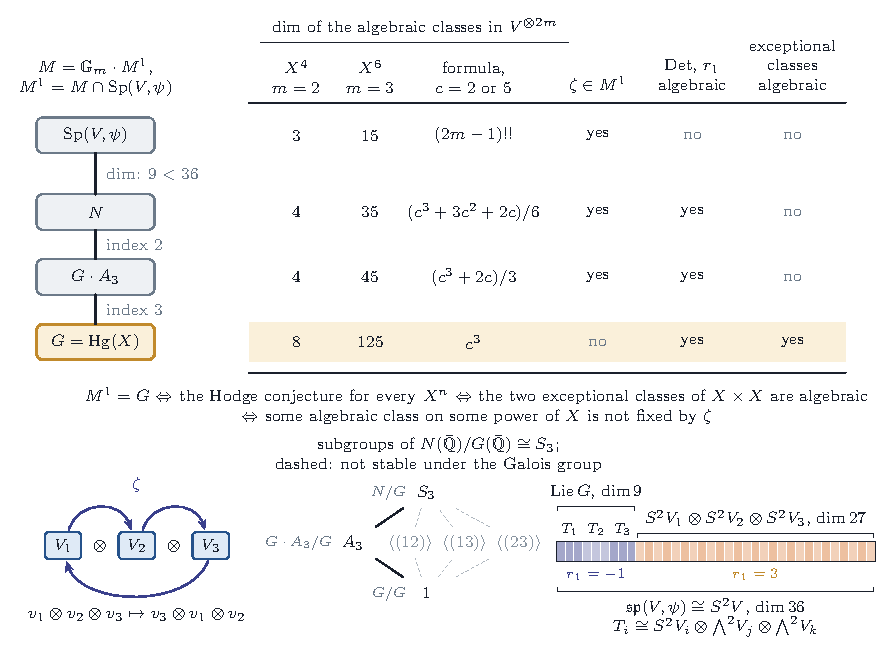
\includegraphics[width=\textwidth]{fig_mumfordgroups}
\caption{The four possible groups $M^{1}=M\cap\Sp(V,\psi)$ of
\Cref{prop:mumfordmotivic}, where $M=\mathbb{G}_{m}\cdot M^{1}$, as the chain
$G\subset G\cdot A_{3}\subset N\subset\Sp(V,\psi)$: the first two inclusions
have index $3$ and $2$, and $N$, whose identity component is $G$, has
dimension $9$ against $36$. For each case the table gives the dimension of
the algebraic classes in the multilinear part $V^{\otimes2m}$ of
$H^{2m}(X^{2m},\QQ)$ for $m=2$ and $m=3$, from the $c=2$, respectively $c=5$,
non-crossing pairings; whether $M^{1}$
contains the cyclic permutation $\zeta$ of the three tensor factors; whether
$\mathrm{Det}$ and $r_{1}$ are algebraic; and whether the two exceptional
classes of $X\times X$ are. Only $M^{1}=G$ makes the exceptional classes
algebraic, and it is equivalent to the Hodge conjecture for every power of
$X$ (\Cref{prop:mumfordmotivic}(ii)); the proposition does not decide which
of the four cases occurs. Below, from left to right: $\zeta$; the subgroups of
$N(\bar{\QQ})/G(\bar{\QQ})\cong S_{3}$, of which only $1$, $A_{3}$ and $S_{3}$
are stable under the Galois group, which acts transitively on the three
factors; and $\mathfrak{sp}(V,\psi)=\operatorname{Lie}G\oplus
S^{2}V_{1}\otimes S^{2}V_{2}\otimes S^{2}V_{3}$, $36=9+27$, the second summand
irreducible under $G$, with the eigenvalues $-1$ and $3$ of $r_{1}$ on the two
summands.}
\label{fig:mumfordgroups}
\end{figure}

The same invariance explains why the classes known or expected to be
algebraic on abelian varieties stop short of the exceptional classes, on all
abelian varieties at once.

\begin{proposition}[The system generated by the known classes]\label{prop:mumfordformal}
Keep \Cref{setup:mumford}, and $\zeta$ and $G\cdot A_{3}$ as in
\Cref{prop:mumfordmotivic}. For an abelian variety $A$ let $A_{X}\subseteq A$
be the largest abelian subvariety isogenous to a power of $X$, and $A'$ the
identity component of the intersection of the kernels of the homomorphisms
$A\to X$. Then $A_{X}\times A'\to A$ is an isogeny, $\Hom(X,A')=0$, and
\[
  H^{1}(A,\QQ)=\bigl(V\otimes\Hom^{0}(A_{X},X)\bigr)\oplus H^{1}(A',\QQ),
\]
the first summand embedded by $v\otimes f\mapsto f^{*}v$. Let $\GL(V)$ act on
$H^{*}(A,\QQ)={\textstyle\bigwedge^{*}}H^{1}(A,\QQ)$ through the factor $V$. Let $\cS$
be the smallest family of subspaces $\cS(A)\subseteq H^{*}(A,\QQ)$, over all
complex abelian varieties $A$, that is closed under linear combinations, cup
products, exterior products, and pull-back and push-forward along
homomorphisms, and contains:
\begin{enumerate}[label=\textup{(\alph*)},leftmargin=2.6em,itemsep=1pt]
\item the divisor classes;
\item for every subfield $E\subseteq\End^{0}(A)$, the rational classes whose
  extension to $\bar{\QQ}$ lies in $\bigoplus_{\sigma}{\textstyle\bigwedge^{d}}
  H^{1}(A,\bar{\QQ})_{\sigma}$, the sum over the embeddings
  $\sigma\colon E\to\bar{\QQ}$ of the top exterior powers of the eigenspaces,
  $d=\dim_{E}H^{1}(A,\QQ)$; among them are the Weil classes;
\item the Hodge classes of the abelian varieties without isogeny factor $X$;
\item the Hodge classes of the powers of $X$ that are fixed by $\zeta$, among
  them $\mathrm{Det}$ and $r_{1}$.
\end{enumerate}
Then every class of $\cS$ is invariant under $G\cdot A_{3}$ acting through
$V$, and the classes obtained from \textup{(a)}, \textup{(b)} and
\textup{(c)} alone are invariant under $\Sp(V,\psi)$. The Hodge classes in
$\cS(X^{m})$ are the Hodge classes of $X^{m}$ fixed by $\zeta$, and $\cS$
contains no exceptional class of $X\times X$.
\end{proposition}

\begin{proof}
Up to isogeny $A=A_{X}\times A'$ by Poincar\'e reducibility, with $A_{X}$
isogenous to some $X^{k}$ and no isogeny factor $X$ in $A'$, so
$\Hom(X,A')=\Hom(A',X)=0$, $X$ being simple. As $\End^{0}(X)=\QQ$,
$\Hom^{0}(A_{X},X)$ has dimension $k$ and the displayed map is an isomorphism.
A homomorphism $h\colon A\to B$ is, up to isogeny, $h_{X}\times h'$ with
$h_{X}\colon A_{X}\to B_{X}$ and $h'\colon A'\to B'$, and $h^{*}$ acts on
$H^{1}$ as $(1\otimes(f\mapsto f\circ h_{X}))\oplus h'^{*}$, which commutes
with $\GL(V)$; so pull-backs are equivariant, and so are cup and exterior
products, $\GL(V)$ acting on $H^{*}(A\times B)=H^{*}(A)\otimes H^{*}(B)$
diagonally. The orientation class of $A$ spans
${\textstyle\bigwedge^{\mathrm{top}}}H^{1}(A)=(\det V)^{\otimes k}\otimes
(\det\Hom^{0}(A_{X},X))^{\otimes8}\otimes{\textstyle\bigwedge^{\mathrm{top}}}H^{1}(A')$, on
which $\SL(V)$ acts trivially, so Poincar\'e duality and push-forwards are
$\SL(V)$-equivariant. Since $G\cdot A_{3}\subseteq\Sp(V,\psi)\subseteq\SL(V)$,
the classes invariant under either group form a family closed under all the
operations, and it remains to look at the generators.

(a) A divisor class of $A$ is the sum of its K\"unneth components in
${\textstyle\bigwedge^{2}}H^{1}(A_{X})$, $H^{1}(A_{X})\otimes H^{1}(A')$ and
${\textstyle\bigwedge^{2}}H^{1}(A')$, which are Hodge classes. The middle one corresponds to a
homomorphism from $A'$ to the dual of $A_{X}$, which is zero. The first is a
Hodge class of $A_{X}$, so a $G$-invariant of ${\textstyle\bigwedge^{2}}(V\otimes\QQ^{k})=
S^{2}V\otimes{\textstyle\bigwedge^{2}}\QQ^{k}\oplus{\textstyle\bigwedge^{2}}V\otimes S^{2}\QQ^{k}$; as
$(S^{2}V)^{G}=0$ and $({\textstyle\bigwedge^{2}}V)^{G}=\QQ\psi$ (proof of
\Cref{thm:lefschetzclosure}(i)), it lies in
$\psi\otimes S^{2}\QQ^{k}$, which $\Sp(V,\psi)$ fixes. On the third $\GL(V)$
acts trivially. (b) The field $E$ acts on $Q=\Hom^{0}(A_{X},X)$ and on
$H^{1}(A')$, and the $\sigma$-eigenspace of $H^{1}(A,\bar{\QQ})$ is
$V\otimes Q_{\sigma}\oplus H^{1}(A',\bar{\QQ})_{\sigma}$. Its top exterior
power is $(\det V)^{\otimes\dim Q_{\sigma}}\otimes(\det Q_{\sigma})^{\otimes8}
\otimes\det H^{1}(A',\bar{\QQ})_{\sigma}$, on which $\SL(V)$ acts trivially.
(c) For such an abelian variety
$A_{X}=0$, and $\GL(V)$ acts trivially. (d) The Hodge classes of $X^{m}$ are
the invariants of $G$, which acts through $V$, and those fixed by $\zeta$ are
invariant under the group $G\cdot A_{3}$ that $G$ and $\zeta$ generate.

So every class of $\cS$ is $G\cdot A_{3}$-invariant, and those obtained from
(a), (b) and (c) are $\Sp(V,\psi)$-invariant. The Hodge classes of $X^{m}$ in
$\cS$ contain those of (d) and are fixed by $\zeta$, so they are exactly the
Hodge classes fixed by $\zeta$; and an exceptional class of $X\times X$ is not
fixed by $\zeta$ (proof of \Cref{prop:mumfordmotivic}(ii)).
\end{proof}

So no argument that uses only these inputs and these operations reaches the
exceptional classes. The inputs include all Weil classes, whether or not they
are known to be algebraic, and with them Markman's cycles \cite{Mar25a}; the
whole Hodge conjecture for the abelian varieties without isogeny factor $X$;
and the algebraicity of $\mathrm{Det}$ and $r_{1}$. A proof needs a cycle
outside this system: on a product of a power of $X$ with an abelian variety, a
class that is not invariant under $G\cdot A_{3}$ acting through $V$, or a cycle
through a variety that is not an abelian variety, such as the Kuga--Satake
class of $S_{\lambda}$ would provide (\Cref{prop:mumfordkslink}).
\Cref{prop:mumfordformal} extends the second limit of
\Cref{rem:mumfordpowersopen}; it is an obstruction to a method, not to the
target, and we claim no priority for it.

The same invariance, used the other way round, shows that the statement (F2)
of \Cref{cor:fourremain} is not smaller than the conjecture for abelian
varieties. For an abelian variety $Y$ let $R(Y)\subseteq H^{*}(Y,\QQ)$ be the
subring generated by divisor classes and Weil classes of quotients, as in
\Cref{rem:f3collapse}.

\begin{proposition}[Statement (F2) is the conjecture for abelian varieties]
\label{prop:f2isab}
Statement \textup{(F2)} of \Cref{cor:fourremain} implies the Hodge
conjecture for every abelian variety, and is therefore equivalent to it.
\end{proposition}

\begin{proof}
The conjecture for abelian varieties contains (F2). For the converse, recall
from \Cref{rem:f3collapse} that (F2) gives every Hodge class of degree $2q$ on
$Y$ as soon as one Hodge class of degree $2q$ on $Y$ lies outside $R(Y)$. Let
$X$ be as in \Cref{setup:mumford}, and let $\zeta$ act on the cohomology of
every abelian variety through the factor $V$, as in \Cref{prop:mumfordformal}.
Every class of $R(Y)$ lies in $\cS(Y)$, so it is fixed by $\zeta$, for every
$Y$; and an exceptional class $e_{0}\in H^{4}(X\times X,\QQ)$ is not
(\Cref{prop:mumfordformal}). Let $\theta$ be an ample class on $X\times X$,
which $\zeta$ fixes. If $\zeta e_{0}=\lambda e_{0}$, then $\lambda\ne1$ and
$e=e_{0}+\theta^{2}$ has $\zeta e=\lambda e_{0}+\theta^{2}$, which is not a
multiple of $e$; otherwise put $e=e_{0}$. In either case $e$ is a Hodge class
of degree $4$ on $X\times X$ with $\zeta e\notin\bar{\QQ}\,e$.

Let $A$ be an abelian variety and $\beta\ne0$ a Hodge class of degree $2p$ on
$A$, and put $Y=A\times X\times X$. As $\zeta$ acts on
$H^{*}(Y)=H^{*}(A)\otimes H^{*}(X\times X)$ diagonally, a class
$\beta\otimes e$ in $R(Y)$ would satisfy
$\zeta\beta\otimes\zeta e=\beta\otimes e$, which forces $\zeta e\in\bar{\QQ}\,e$.
So the Hodge class $\beta\otimes e$ lies outside $R(Y)$, and (F2) makes it
algebraic. In the same way $e\cup\theta^{4}\notin R(X\times X)$, since
otherwise $(\zeta e-e)\cup\theta^{4}=0$ and the hard Lefschetz theorem would
give $\zeta e=e$; so (F2) makes every Hodge class of degree $12$ on
$X\times X$ algebraic. By the Hodge--Riemann bilinear relations the
intersection pairing between the Hodge classes of degrees $4$ and $12$ on
$X\times X$ is nondegenerate, so there is a Hodge class $e'$ of degree $12$
with $\int_{X\times X}e\cup e'=1$. Then
\[
  \beta=\mathrm{pr}_{A*}\bigl((\beta\otimes e)\cup
  \mathrm{pr}_{X\times X}^{*}e'\bigr),
\]
with $\mathrm{pr}_{A}$ and $\mathrm{pr}_{X\times X}$ the projections of $Y$,
and $\beta$ is algebraic.
\end{proof}

\begin{remark}[The rule set with \Cref{prop:f2isab}]\label{rem:f2rule}
\Cref{thm:closure} is a statement about the rule set of \Cref{setup:rules},
and \Cref{prop:f2isab} is a rule that the set does not contain. Adjoined to
it, the rule changes the fifth minimal set of \Cref{thm:closure}(ii): the
minimal sufficient sets become
\[
  \{\mathrm{F3}\},\quad\{\mathrm{L},\mathrm{M}\},\quad
  \{\mathrm{L},\mathrm{F3}'\},\quad\{\mathrm{V},\mathrm{F3}'\},\quad
  \{\mathrm{F2},\mathrm{F3}'\},
\]
and $\mathrm{P2}_{\mathrm{split}}$ lies in none of them. Indeed the new rule
has the premise (F2) and the conclusion $\mathbf{AB}$, the conjecture for
abelian varieties, so the sets $C_{1}$, $C_{2}$ and $C_{4}$ of the proof of
\Cref{thm:closure} stay closed, and a sufficient set meets $H_{1}$, $H_{2}$
and $H_{4}$. The sets meeting these three that are minimal with this property
are the five above, by the argument of that proof without $H_{3}$, and each is
sufficient: $\{\mathrm{F2},\mathrm{F3}'\}$ gives $\mathbf{AB}$ by the new
rule and then $\mathbf{HC}$ by \Cref{prop:f3prime}(i). So the results of this
paper on Weil classes do not shorten a route to the conjecture. What they do
is reduce one case of it, the algebraicity of the Weil classes of every CM
field, to the single statement $\mathrm{P2}_{\mathrm{split}}$, by a route that
does not pass through (F2). Like (F3), which is the whole conjecture, (F2) is
the whole conjecture for abelian varieties, carried by the classes that are
hardest to reach; the exceptional classes of $X\times X$ are its smallest
instance, and the proof above shows that the classes $\beta\otimes e$ built
from them already carry all of it.
\end{remark}

\section{The main theorem in every family}\label{sec:families}

\Cref{thm:main} describes the algebraic locus of the Weil classes in one
family: it contains an explicit CM point, it is dense, it is a countable union
of closed algebraic strata, and it is the whole family as soon as it has an
interior point. The first two properties use the Weil classes; the last two
hold for every flat class on every smooth projective family
(\Cref{lem:algstrata}). This section carries the theorem to the families that
carry (F2) and
\textup{(F3$'$)}, and records what each construction of the paper
contributes there.

For (F2) the families are abelian schemes with a member of CM type. Every
Hodge class of every abelian variety lies in such a family
(\Cref{prop:cmfamily}), and (F2) is equivalent to the statement that in every
one of them the algebraic locus of a flat Hodge class that is algebraic at a
CM member has an interior point (\Cref{thm:f2propagation}). The base points
of \Cref{thm:cmbasepoint} are the CM seeds of the Weil families, and
Andr\'e's theorem makes the Weil classes of the split families seeds for every
Hodge class of CM type. For \textup{(F3$'$)} the cohomology of a variety splits
into the part reached from abelian varieties by algebraic correspondences and
a complement, and \textup{(F3$'$)} is the statement that the complement
carries no Hodge class (\Cref{prop:abpart}). On the first varieties where
\textup{(F3$'$)} is open, the squares of K3 surfaces with real
multiplication, the algebraic locus of the real multiplication contains every
CM point, is dense and stable under a group of rational Hodge isometries, and
is either everything or meagre (\Cref{thm:rmlocus}). In both cases what is
left is the interior point, and \Cref{thm:twostand} lists what the
constructions of the paper give towards it.

\subsection{Algebraic loci}\label{ssec:algloci}

\begin{definition}[Algebraic locus]\label{def:algloc}
Let $S$ be a smooth connected complex quasi-projective variety,
$f\colon\cX\to S$ a smooth projective morphism, and $\xi$ a global section of
$R^{2p}f_{*}\QQ$ over $S^{\mathrm{an}}$.\footnote{By Ehresmann's theorem $f$
is a locally trivial fibration of differentiable manifolds, so
$R^{2p}f_{*}\QQ$ is a local system with fibre $H^{2p}(\cX_{s},\QQ)$ at $s$. A
global section is a class $\xi_{s}$ on every fibre that is locally constant
under the identifications of nearby fibres, equivalently a class on one fibre
fixed by the monodromy. The set of points $s$ at which $\xi_{s}$ is of type
$(p,p)$ is in general a proper subset of $S$, and it is algebraic by
\Cref{thm:cdk}.} The \emph{algebraic locus} of $\xi$
is
\[
  \Sigma(\xi)=\{\,s\in S:\ \xi_{s}\ \text{is the class of an algebraic cycle
  with rational coefficients on}\ \cX_{s}\,\}.
\]
\end{definition}

\begin{lemma}[The dichotomy in every family]\label{lem:algstrata}
In \Cref{def:algloc} the following hold.
\begin{enumerate}[label=\textup{(\roman*)},leftmargin=2.6em,itemsep=2pt]
\item $\Sigma(\xi)$ is the union of countably many Zariski closed subsets of
  $S$.
\item Either $\Sigma(\xi)=S$, or $\Sigma(\xi)$ is meagre in $S^{\mathrm{an}}$.
\item The following are equivalent: $\Sigma(\xi)=S$; $\Sigma(\xi)$ has an
  interior point; $\Sigma(\xi)$ is not meagre; $\xi_{s}$ is algebraic for
  every $s$ outside a countable union of proper closed analytic subsets of
  $S$. If $\Sigma(\xi)$ is dense, they are also equivalent to $\Sigma(\xi)$
  being closed.
\end{enumerate}
\end{lemma}

\begin{proof}
(i) The proof of \Cref{thm:closedlocus} applies with
$(\cA,\cS,\omega)$ replaced by $(\cX,S,\xi)$, as in \Cref{lem:spreading}:
for a tuple $\underline{P}$ of Hilbert polynomials the fibre product of the
relative Hilbert schemes $\Hilb^{P_{i}}(\cX/S)$ is projective over $S$
\cite{Gro61}, the class of a flat family of cycles is a flat section, two flat
sections over a connected base that agree at one point agree everywhere, and
the image of a proper morphism is closed. So the set of points at which
$\xi_{s}=\sum_{i}q_{i}[Z_{i}]$ with $Z_{i}$ of Hilbert polynomial $P_{i}$ is
Zariski closed, and $\Sigma(\xi)$ is the union of these strata over the
countably many pairs $(\underline{P},\underline{q})$.

(ii) and (iii). A Zariski closed subset of the irreducible variety $S$ that
has an interior point in $S^{\mathrm{an}}$ is all of $S$, and a proper one is
nowhere dense. If no stratum is $S$, then $\Sigma(\xi)$ is a countable union
of nowhere dense closed sets, hence meagre, and has no interior point, since
$S^{\mathrm{an}}$ is a Baire space. If one stratum is $S$, then
$\Sigma(\xi)=S$. This gives (ii) and the equivalence of the first three
conditions of (iii). The complement of a countable union of proper closed
analytic subsets is not meagre, by the Baire category theorem, so the fourth
condition implies the third, and it is implied by the first. Finally, a
dense set that is closed is $S$.
\end{proof}

So the dichotomy of \Cref{thm:main}(iii) and the equivalences of
\Cref{thm:main}(iv) hold for every flat class on every smooth projective
family; what \Cref{thm:main} adds for the Weil classes is a point of
$\Sigma(\xi)$ and the density, and neither is automatic, since
$\Sigma(\xi)$ may be empty.

\subsection{(F2) is propagation from CM points}\label{ssec:f2cm}

\begin{lemma}[Points of CM type are dense]\label{lem:cmdense}
Let $G$ be a connected reductive group over $\QQ$, let
$u_{0}\colon\mathrm{U}(1)\to G_{\RR}$ be a homomorphism, and let $\cD$ be
the orbit of $u_{0}$ under conjugation by $G(\RR)^{+}$, with the topology of
$G(\RR)^{+}/\mathrm{Stab}(u_{0})$. Then the points $u\in\cD$ for which
$u(\mathrm{U}(1))\subseteq T_{\RR}$ for some maximal torus $T$ of $G$ defined
over $\QQ$ are dense in $\cD$.
\end{lemma}

\begin{proof}
Let $u_{1}\in\cD$ and let $W$ be a neighbourhood of $u_{1}$. The centraliser
of the torus $u_{1}(\mathrm{U}(1))$ in $G_{\RR}$ is connected and reductive,
and a maximal torus of it defined over $\RR$ is a maximal torus $T_{1}$ of
$G_{\RR}$ containing $u_{1}(\mathrm{U}(1))$. Write $\mathfrak{g}$ for the Lie
algebra of $G$ and $\mathfrak{t}_{1}\subseteq\mathfrak{g}_{\RR}$ for that of
$T_{1}$, and choose a regular element $Y_{1}\in\mathfrak{t}_{1}$. The map
$\varphi\colon G(\RR)^{+}\times\mathfrak{t}_{1}\to\mathfrak{g}_{\RR}$,
$(g,Y)\mapsto\mathrm{Ad}(g)Y$, has differential
$(Z,Y')\mapsto[Z,Y_{1}]+Y'$ at $(1,Y_{1})$, which is onto because
$\mathfrak{g}_{\RR}=\mathfrak{t}_{1}\oplus[\mathfrak{g}_{\RR},Y_{1}]$ for a
regular semisimple $Y_{1}$. So for neighbourhoods $N_{1}$ of $1$ in
$G(\RR)^{+}$ with $N_{1}u_{1}N_{1}^{-1}\subseteq W$, and $N_{2}$ of $Y_{1}$
in $\mathfrak{t}_{1}$ consisting of regular elements, the image
$\varphi(N_{1}\times N_{2})$ contains a nonempty open subset of
$\mathfrak{g}_{\RR}$. The rational points $\mathfrak{g}(\QQ)$ are dense in
$\mathfrak{g}_{\RR}$, so that open subset contains some
$Y\in\mathfrak{g}(\QQ)$, and $Y=\mathrm{Ad}(g)Y'$ with $g\in N_{1}$ and
$Y'\in N_{2}$. As $Y$ is rational and regular semisimple, the identity
component $T$ of its centraliser in $G$ is a maximal torus defined over
$\QQ$, and $T_{\RR}=gT_{1}g^{-1}$ because the centraliser of $Y'$ has
identity component $T_{1}$. Then $u=gu_{1}g^{-1}$ lies in $W$ and
$u(\mathrm{U}(1))\subseteq T_{\RR}$.
\end{proof}

For an abelian variety the lemma is used with $G$ its Hodge group, the
smallest algebraic $\QQ$-subgroup of $\GL(H^{1}(A,\QQ))$ whose real points
contain the image of the homomorphism $\mathrm{U}(1)\to\GL(H^{1}(A,\RR))$
that defines the Hodge structure. If $\Hg(A)$ lies in a $\QQ$-torus $T$, then
$A$ is of CM type.\footnote{For an elliptic curve $G=\SL_{2}$ and $\cD$ is
the upper half-plane. The compact torus $u_{\tau}(\mathrm{U}(1))$ fixing
$\tau$ lies in the real points of a maximal $\QQ$-torus of $\SL_{2}$ exactly
when $\tau$ is imaginary quadratic, and the torus is then the group of
elements of norm one of $\QQ(\tau)$. So the points of \Cref{lem:cmdense}
are the curves with complex multiplication, and the lemma is the familiar
density of the imaginary quadratic points in the upper half-plane.} Indeed $T$ lies in a maximal $\QQ$-torus $T'$ of
$\GL(H^{1}(A,\QQ))$, which is the group of units of a commutative semisimple
$\QQ$-subalgebra $L\subseteq\End(H^{1}(A,\QQ))$ of dimension $2\dim A$; the
algebra $L$ commutes with $T'\supseteq\Hg(A)$, so it lies in the commutant of
$\Hg(A)$, which is $\End^{0}(A)$.

\begin{proposition}[A family with a CM member through every Hodge
class]\label{prop:cmfamily}
Let $A_{0}$ be a complex abelian variety and $\gamma$ a Hodge class of degree
$2p$ on $A_{0}$. There are a smooth connected complex quasi-projective variety
$S$, a polarised abelian scheme $\pi\colon\cA\to S$, a global section $\xi$ of
$R^{2p}\pi_{*}\QQ$ that is a Hodge class at every point, and points $s_{0}$,
$c\in S$, such that $\cA_{s_{0}}\cong A_{0}$ with $\xi_{s_{0}}=\gamma$ under
this isomorphism and $\cA_{c}$ is of CM type.
\end{proposition}

\begin{proof}
Let $\ell\ge1$ be an integer with $\ell\gamma$ integral. We construct a
section with value $\ell\gamma$ at $s_{0}$ and divide it by $\ell$ at the
end; until then $\gamma$ stands for $\ell\gamma$. Fix a polarisation of
$A_{0}$, put $V=H_{1}(A_{0},\QQ)$, and fix a level $N\ge3$. As in \Cref{setup:shimura}, the
quotient $\cS_{g}$ of the Siegel space $\cH$ of complex structures on
$V_{\RR}$ compatible with the polarisation, by the principal congruence
subgroup of level $N$ of the stabiliser of $H_{1}(A_{0},\ZZ)$, is a smooth
quasi-projective variety carrying a universal family $f\colon\cA_{g}\to\cS_{g}$,
polarised by the fixed polarisation \cite{BB66}; let $a_{0}\in\cS_{g}$ be the
point of $A_{0}$ and $J_{0}\in\cH$ a lift, through which the fibre of
$R^{2p}f_{*}\ZZ$ at every point of the image of $\cH$ is identified with
$H^{2p}(A_{0},\ZZ)=\bigwedge^{2p}H_{1}(A_{0},\ZZ)^{\vee}$ by parallel
transport in the simply connected space $\cH$. Put
$\mathbb{V}=R^{2p}f_{*}\ZZ$, a polarised variation of $\ZZ$-Hodge
structure. By \Cref{thm:cdk} the connected component $\mathcal{C}$ of its
locus of Hodge classes that contains $(a_{0},\gamma)$ is a closed algebraic
subvariety of the total space of $\mathbb{V}$; it has finitely many
irreducible components.

Let $G=\Hg(A_{0})$, which lies in the symplectic group of the polarisation
and fixes $\gamma$ \cite[\S3]{Del82}, let
$u_{0}\colon\mathrm{U}(1)\to G_{\RR}$,
$u_{0}(e^{i\theta})=\cos\theta+J_{0}\sin\theta$, be the homomorphism defining
the Hodge structure, and let
$\cD=\{gJ_{0}g^{-1}:g\in G(\RR)^{+}\}$. For $g\in G(\RR)^{+}$ the complex
structure $J=gJ_{0}g^{-1}$ is compatible with the polarisation and positive
for it, since $g$ preserves the polarisation, so $\cD\subseteq\cH$; and
$\cD$ is the orbit of \Cref{lem:cmdense} when $J$ is identified with
$u_{J}=gu_{0}g^{-1}$. For $J\in\cD$ the group $u_{J}(\mathrm{U}(1))$ lies in
$G(\RR)$, so $\Hg(A_{J})\subseteq G$ fixes $\gamma$, which is therefore a
Hodge class on $A_{J}$. The map sending $J\in\cD$ to the image of $J$ in
$\cS_{g}$ together with $\gamma$ is thus a continuous map from the
connected space $\cD$ to the locus of Hodge classes of $\mathbb{V}$, so it
takes values in $\mathcal{C}$. By \Cref{lem:cmdense} there are points
$J_{k}\in\cD$ converging to $J_{0}$ with $u_{J_{k}}(\mathrm{U}(1))$ in the
real points of a $\QQ$-torus of $G$; then $\Hg(A_{J_{k}})$ lies in that torus
and $A_{J_{k}}$ is of CM type. One of the finitely many irreducible
components of $\mathcal{C}$, say $\mathcal{C}_{0}$, contains the images of
infinitely many $J_{k}$, and, being closed, also their limit $(a_{0},\gamma)$.

Let $\rho\colon S\to\mathcal{C}_{0}$ be a resolution of singularities
\cite{Hir64}: $S$ is smooth, connected and quasi-projective, since
$\mathcal{C}_{0}$ is irreducible and quasi-projective, and $\rho$ is
projective and surjective. Let $\pi\colon\cA\to S$ be the pull-back of
$\cA_{g}$ along $S\to\mathcal{C}_{0}\to\cS_{g}$, a polarised abelian scheme.
A point of $\mathcal{C}_{0}$ is a pair $(a,v)$ with $v\in\mathbb{V}_{a}$ of
Hodge type, and $(a,v)\mapsto v$ is a flat section of the pull-back of
$\mathbb{V}$ to $\mathcal{C}_{0}$, because the total space of a local system
is a covering space of the base; its pull-back to $S$, divided by $\ell$, is
a flat section $\xi$ of $R^{2p}\pi_{*}\QQ$ of Hodge type at every point.
Take $s_{0}$ over $(a_{0},\gamma)$ and $c$ over the image of some $J_{k}$ in
$\mathcal{C}_{0}$.
\end{proof}

\begin{theorem}[(F2) is propagation from CM points]\label{thm:f2propagation}
The following are equivalent.
\begin{enumerate}[label=\textup{(\roman*)},leftmargin=2.6em,itemsep=2pt]
\item \textup{(F2)}.
\item The Hodge conjecture holds for every complex abelian variety.
\item For every polarised abelian scheme $\pi\colon\cA\to S$ over a smooth
  connected complex quasi-projective variety and every global section $\xi$
  of $R^{2p}\pi_{*}\QQ$, if $\xi_{s}$ is algebraic at one point $s\in S$,
  then $\Sigma(\xi)=S$.
\item The same, for the points $s$ at which $\cA_{s}$ is of CM type: if
  $\xi_{c}$ is algebraic at one point $c$ with $\cA_{c}$ of CM type, then
  $\Sigma(\xi)=S$.
\item For every $\pi$ and $\xi$ as in \textup{(iii)} with $\xi_{c}$ algebraic
  at a point $c$ with $\cA_{c}$ of CM type, $\Sigma(\xi)$ has an interior
  point.
\end{enumerate}
\end{theorem}

\begin{proof}
(i) and (ii) are equivalent by \Cref{prop:f2isab}. If (ii) holds and
$\xi_{s}$ is algebraic, then $\xi_{t}$ is a Hodge class at every $t$ by the
first part of the proof of \Cref{prop:lefvhc}, which uses only the theorem of
the fixed part and the semisimplicity of polarisable Hodge structures, and it
is algebraic by (ii); so (ii) implies (iii). (iv) is the case of (iii) at
points of CM type, and
(iv) and (v) are equivalent by \Cref{lem:algstrata}(iii).

Assume (iv). Let $F$ be a CM field and $n\ge2$, and let $\delta_{0}$ be the
trivial class, the discriminant of a hermitian space that is a sum of $n$
hyperbolic planes, each of determinant $-1$. The family of
$(F,n,\delta_{0})$-Weil type over its Shimura variety with a level structure,
as in \Cref{setup:cmfield} and \Cref{setup:shimura}, is a polarised abelian
scheme over a smooth connected quasi-projective base, on which the Weil
classes are global sections (\Cref{prop:cmweil}(i)). By \Cref{thm:main}(i)
they are algebraic at a member isogenous to a product of abelian varieties
with complex multiplication by $F$, which is of CM type, and by (iv) they are
algebraic at every member. Let $A$ be an abelian variety of split Weil type
for $F$ in the sense of \cite[\S2.1]{Mil20}: $F$ acts on it with
$\dim_{F}H^{1}(A,\QQ)=2n$ and $\dim V_{\sigma}^{1,0}=n$ for every embedding
$\sigma$, and for some polarisation the hermitian form of
\Cref{rem:cmmember} has a totally isotropic subspace of dimension $n$, so
that it is a sum of $n$ hyperbolic planes and $A$ is of
$(F,n,\delta_{0})$-Weil type. By \Cref{prop:cmweil}(iv) the Hodge structure
$H^{1}(A,\QQ)$ is isomorphic, compatibly with $F$, to that of a member $A_{s}$
of the family, so there is an isogeny $A\to A_{s}$ commuting with $F$; its
pull-back maps $W_{F}(A_{s})$ onto $W_{F}(A)$ and algebraic classes to
algebraic classes. So every abelian variety of split Weil type has algebraic
Weil classes, for $n\ge2$ by this argument and for $n=1$ by the theorem of
Lefschetz on $(1,1)$ classes. By Andr\'e's theorem
\cite[Theorem~1 and its proof]{Mil20}, every Hodge class on an abelian
variety $B$ of CM type is a sum $\sum f_{\Delta}^{*}(t_{\Delta})$ of
pull-backs along homomorphisms $f_{\Delta}\colon B\to A_{\Delta}$ of Weil
classes $t_{\Delta}$ on abelian varieties $A_{\Delta}$ of split Weil type
for CM fields $F_{\Delta}$; so the Hodge conjecture holds for every abelian
variety of CM type. Now let $A_{0}$ be any abelian variety and $\gamma$ a
Hodge class on it, and take $S$, $\pi$, $\xi$, $s_{0}$, $c$ from
\Cref{prop:cmfamily}. Then $\xi_{c}$ is algebraic, so by (iv)
$\xi_{s_{0}}=\gamma$ is algebraic. This is (ii).
\end{proof}

\Cref{fig:cmseed} draws the theorem in one family.

The implication from \textup{(iii)} to \textup{(ii)} is the argument of
Deligne and Andr\'e as Milne records it \cite[\S5, Theorem~3 and
Remark~2]{Mil20}.\footnote{Deligne's proof that Hodge classes on abelian
varieties are absolutely Hodge uses families of the same kind \cite{Del82}.
By his Principle B \cite[\S2]{Del82} the property of being absolutely Hodge
passes from one member of a family to every member, so a family through a
given Hodge class with a member of CM type reduces the question to that
member. Algebraicity is not known to pass from one member to all, and
\textup{(iii)} is precisely that property.} In that argument the families can be taken to be polarised
abelian schemes and the starting points to be of CM type, which is what
\textup{(iv)} records, and the converse holds. The seeds
are explicit: for the Weil classes they are the base points of
\Cref{thm:cmbasepoint}, and for every other Hodge class they are the CM
members supplied by \Cref{prop:cmfamily}, at which the class is algebraic once
the Weil classes of the split families are. For the Weil classes of the
split family of a CM field, whose base point is of CM type, statement
\textup{(v)} is the condition of \Cref{thm:main}(iv). So the condition of
\Cref{thm:main}(iv), required in every polarised abelian scheme with a
member of CM type at which the class is algebraic, is exactly (F2); it is not a reduction
of (F2) to something smaller, because the interior point it asks for is the
conclusion of \textup{(iii)}.

\begin{figure}[tbp]
\centering
  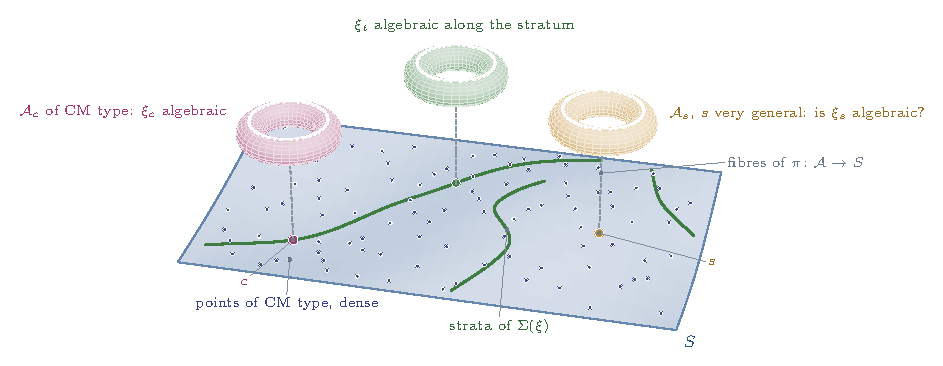
\includegraphics[width=\textwidth]{fig_cmseed}
\caption{\Cref{thm:f2propagation} in one family. The sheet is the base $S$
of a polarised abelian scheme $\pi\colon\cA\to S$ through a given Hodge
class, as in \Cref{prop:cmfamily}; the small dots are its points of CM type,
dense by \Cref{lem:cmdense}, and the green curves are strata of the algebraic
locus $\Sigma(\xi)$ of the flat class $\xi$ (\Cref{lem:algstrata}). Above
three points the fibres are drawn as tori, and the loop on each stands for
$\xi$, carried from fibre to fibre by parallel transport. At the CM member
$\cA_{c}$ the class is algebraic, and it stays algebraic along the stratum
through $c$. At a very general member $\cA_{s}$ it is algebraic exactly when
$\Sigma(\xi)$ has an interior point, and (F2) is the statement that this
happens in every such family.}
\label{fig:cmseed}
\end{figure}

\subsection{(F3$'$) and the part reached from abelian varieties}
\label{ssec:abpart}

\begin{definition}[The abelian part]\label{def:abpart}
For a smooth complex projective variety $X$ and $p\ge0$ let
$H^{2p}_{\mathrm{ab}}(X)\subseteq H^{2p}(X,\QQ)$ be the sum of the images of
the maps
$\Gamma_{*}\colon H^{k}(B,\QQ)\to H^{2p}(X,\QQ)$,
$y\mapsto\mathrm{pr}_{X*}([\Gamma]\cup\mathrm{pr}_{B}^{*}y)$, over all
complex abelian varieties $B$, the point included, all $k$, and all algebraic
cycles $\Gamma$ on $B\times X$ with rational coefficients and of the
codimension that lands in degree $2p$.
\end{definition}

\begin{proposition}[\textup{(F3$'$)} is a statement about the complement of
the abelian part]\label{prop:abpart}
Let $X$ be a smooth complex projective variety and $p\ge0$.
\begin{enumerate}[label=\textup{(\roman*)},leftmargin=2.6em,itemsep=2pt]
\item $H^{2p}_{\mathrm{ab}}(X)$ is a sub-Hodge structure of
  $H^{2p}(X,\QQ)$, spanned by the images of finitely many of the maps
  $\Gamma_{*}$.
\item $\mathrm{Ab}^{p}(X)=\Hdg^{p}(X)\cap H^{2p}_{\mathrm{ab}}(X)$.
\item Let $T^{2p}_{\mathrm{ab}}(X)$ be a complement of
  $H^{2p}_{\mathrm{ab}}(X)$ in $H^{2p}(X,\QQ)$ as a Hodge structure. Then
  \textup{(F3$'$)} holds for $X$ in degree $2p$ if and only if
  $T^{2p}_{\mathrm{ab}}(X)$ contains no nonzero Hodge class, in particular
  whenever the Hodge group of $T^{2p}_{\mathrm{ab}}(X)$ fixes no nonzero
  vector.
\item $X$ lies in the class $\mathcal{A}$ of \Cref{prop:f3prime}(iii) if and
  only if $T^{2p}_{\mathrm{ab}}(X)=0$ for every $p$ and the odd cohomology is
  reached in the same way.
\end{enumerate}
\end{proposition}

\begin{proof}
(i) An algebraic cycle $\Gamma$ of codimension $e$ on $B\times X$, with
$\dim B=b$, induces a morphism of Hodge structures
$H^{k}(B,\QQ)\to H^{k+2e-2b}(X,\QQ)(e-b)$, so its image is a sub-Hodge
structure; a sum of sub-Hodge structures is one, and a finite-dimensional
space is spanned by finitely many of them.

(ii) Every $\Gamma_{*}\beta$ with $\beta$ a Hodge class lies in both sets, so
$\mathrm{Ab}^{p}(X)$ is contained in the intersection. Conversely take
$(B_{j},\Gamma_{j},k_{j})$, $1\le j\le r$, as in (i), and let
\[
  \Phi=\sum_{j}\Gamma_{j*}\colon
  \bigoplus_{j}H^{k_{j}}(B_{j},\QQ)(t_{j})\longrightarrow
  H^{2p}_{\mathrm{ab}}(X),
\]
with the Tate twists $t_{j}$ that make it a morphism of pure Hodge structures
of weight $2p$; it is surjective. Polarisable Hodge structures form a
semisimple category, so $\Phi$ has a section $\sigma$ that is a morphism of
Hodge structures. For a Hodge class $\gamma\in H^{2p}_{\mathrm{ab}}(X)$ the
class $\sigma(\gamma)$ is of type $(p,p)$, so each component
$\beta_{j}\in H^{k_{j}}(B_{j},\QQ)$ is a Hodge class, $k_{j}$ being even, and
$\gamma=\sum_{j}\Gamma_{j*}\beta_{j}\in\mathrm{Ab}^{p}(X)$.

(iii) A complement exists by semisimplicity, and the Hodge classes of
$H^{2p}(X,\QQ)$ are the sums of those of the two summands; by (ii) the
Hodge classes of the first summand are $\mathrm{Ab}^{p}(X)$. So
$\Hdg^{p}(X)=\mathrm{Ab}^{p}(X)$ exactly when the second has none, and a
Hodge class of $T^{2p}_{\mathrm{ab}}(X)$ is a vector fixed by its Hodge group
\cite[\S3]{Del82}. (iv) is the definition of $\mathcal{A}$ read degree by
degree.
\end{proof}

So \textup{(F3$'$)} asks nothing of the abelian part, where by (ii) and
\Cref{prop:f2isab} the Hodge conjecture reduces to (F2), and it asks of the
complement that it carry no Hodge class. The abelian part contains every
algebraic class, taking $B$ a point, so under the Hodge conjecture the
complement carries none. To prove \textup{(F3$'$)} for $X$ in degree $2p$
without it, one has to show that every Hodge class of $X$ is a sum of
classes $\Gamma_{*}\beta$, that is, to construct algebraic cycles $\Gamma$
on products $B\times X$ that reach it, which is the step
\Cref{rem:f3primeopen} isolates.
\Cref{prop:f3prime}(iii), \Cref{prop:aclosure} and \Cref{thm:simplextype}
are cases in which the complement is zero, and \Cref{prop:k3powers} and
\Cref{prop:k3ntype} cases in which the conjecture itself makes its Hodge
classes algebraic.

\subsection{The first open case of (F3$'$) in families}\label{ssec:rmlocus}

The frontier of \textup{(F3$'$)} in \Cref{rem:f3primefrontier} begins with
$S\times S$ and $S^{[2]}$ for a K3 surface $S$ with real multiplication. These
surfaces come in families over Hermitian symmetric domains, and the argument
of \Cref{thm:main} applies to them with rational Hodge isometries in place of
isogenies.

\begin{setupenv}[A family with real multiplication]\label{setup:rm}
\enlargethispage{2pt}%
Let $E$ be a totally real field of degree $r\ge2$ and $T$ a finite-dimensional
$\QQ$-vector space with an action of $E$ and a nondegenerate symmetric form
$q$ for which $E$ acts by self-adjoint maps, so that $q=\Tr_{E/\QQ}q_{E}$ for
a unique $E$-bilinear form $q_{E}$. Put $m=\dim_{E}T\ge3$, and suppose that
$q_{E}$ has signature $(2,m-2)$ at one real place $\sigma_{1}$ of $E$ and is
negative definite at the others, and that $(T,q)$ embeds isometrically in
$\Lambda_{\QQ}$, where $\Lambda$ is the K3 lattice; write
$N=T^{\perp}\cap\Lambda$. Let $T_{1}=T\otimes_{E,\sigma_{1}}\RR$ and
\[
  \cD_{E}=\{\,[\omega]\in\PP(T_{1}\otimes_{\RR}\CC):\ q(\omega,\omega)=0,\
  q(\omega,\bar\omega)>0\,\}^{+},
\]
one of its two components, a bounded symmetric domain of dimension $m-2$. For
$\omega\in\cD_{E}$ let $S_{\omega}$ be a K3 surface with a marking
$H^{2}(S_{\omega},\ZZ)\cong\Lambda$ carrying $H^{2,0}(S_{\omega})$ to
$\CC\omega$, which exists by the surjectivity of the period map
\cite[Chs.~6--7]{Huy16}; it is projective, since $N$ has signature
$(1,21-rm)$ and so contains a class of positive square, which is of type
$(1,1)$ \cite[Ch.~8]{Huy16}. Each $e\in E$ acts on
$T_{1}\otimes\CC$ by the scalar $\sigma_{1}(e)$ and is self-adjoint, so it
preserves the Hodge decomposition of $T$, and $T\subseteq H^{2}(S_{\omega},\QQ)$
is a sub-Hodge structure containing $T(S_{\omega})_{\QQ}$. Write
$\tilde e_{\omega}\in H^{4}(S_{\omega}\times S_{\omega},\QQ)$ for the class of
the endomorphism $e\oplus0$ of $H^{2}(S_{\omega},\QQ)=T\oplus N_{\QQ}$, a
Hodge class, and let
\[
  \Sigma_{E}=\{\,\omega\in\cD_{E}:\ \tilde e_{\omega}\ \text{is algebraic
  for every}\ e\in E\,\}
\]
be the algebraic locus of the real multiplication; as $e\mapsto\tilde
e_{\omega}$ is $\QQ$-linear, it suffices to ask this for $e$ in a $\QQ$-basis
of $E$. The set $\Sigma_{E}$ does not depend on the choice of the surfaces
$S_{\omega}$. If $(S,\varphi)$ and $(S',\varphi')$ are two marked choices
for $\omega$, then $\psi=\varphi'^{-1}\varphi$ is a rational Hodge isometry
$H^{2}(S,\QQ)\to H^{2}(S',\QQ)$, induced by an algebraic class $Z$ on
$S\times S'$ by Buskin's theorem \cite{Bus19}, and $Z^{t}$ induces the
adjoint $\psi^{-1}$; the composite $Z\circ\tilde e\circ Z^{t}$ acts on
$H^{2}(S',\QQ)$ as $\psi(e\oplus0)\psi^{-1}$, which is $e\oplus0$ for the
marking $\varphi'$, and by zero on $H^{0}$ and $H^{4}$, so it is the class
$\tilde e'$ of $S'$, and $\tilde e$ is algebraic if and only if $\tilde e'$
is. Let $G=\Res_{E/\QQ}\SO(T,q_{E})$, so that
$G(\RR)=\SO(T_{1})\times\prod_{\sigma\ne\sigma_{1}}\SO(T_{\sigma})$; write
$G(\RR)^{+}$ for the identity component of this Lie group, which acts
transitively on $\cD_{E}$ through its first factor, and
$\Gamma_{\QQ}=G(\QQ)\cap G(\RR)^{+}$.
\end{setupenv}

The surfaces with real multiplication of \cite{vG08,vGS25} lie in families
of this kind,\footnote{For a projective K3 surface $S$ the transcendental
part $T(S)_{\QQ}$ is an irreducible Hodge structure whose algebra of Hodge
endomorphisms is a field, totally real or CM \cite{Zar83}; $S$ has real
multiplication when this field is totally real and not $\QQ$. The space
$T(S)_{\QQ}$ is then a vector space over the field, so its degree divides
$\dim T(S)_{\QQ}$, and a very general member of a family of
\Cref{setup:rm} has $T(S_{\omega})_{\QQ}=T$ and real multiplication by
exactly $E$, as the proof of \Cref{thm:rmlocus} shows.} and so do the surfaces $S_{\lambda}$ of \Cref{thm:mumfordks},
for which $E$ is cubic, $m=3$ and $\cD_{E}$ is a disc.

\begin{theorem}[The algebraic locus of a real multiplication]
\label{thm:rmlocus}
Keep \Cref{setup:rm}.
\begin{enumerate}[label=\textup{(\roman*)},leftmargin=2.6em,itemsep=2pt]
\item The points $\omega$ at which $S_{\omega}$ has complex multiplication,
  that is, at which the Hodge group of $T(S_{\omega})_{\QQ}$ is commutative,
  are dense in $\cD_{E}$, and they lie in $\Sigma_{E}$.
\item $\Sigma_{E}$ is stable under $\Gamma_{\QQ}$, and $\Gamma_{\QQ}$ is dense
  in $G(\RR)^{+}$.
\item $\Sigma_{E}$ is dense in $\cD_{E}$, and either $\Sigma_{E}=\cD_{E}$ or
  $\Sigma_{E}$ is meagre.
\item The following are equivalent: $\Sigma_{E}$ is closed; $\Sigma_{E}$ has
  an interior point; $\Sigma_{E}$ is not meagre; $\Sigma_{E}=\cD_{E}$; the
  Hodge conjecture holds for $S_{\omega}\times S_{\omega}$ for every $\omega$
  outside a countable union of proper closed analytic subsets of $\cD_{E}$.
  When they hold, the Hodge conjecture and \textup{(F3$'$)} hold for
  $S_{\omega}\times S_{\omega}$ and $S_{\omega}^{[2]}$ at every $\omega$ at
  which $\End_{\mathrm{Hdg}}(T(S_{\omega})_{\QQ})$ is $E$ or a CM field.
\end{enumerate}
\end{theorem}

\begin{proof}
We first record two facts about the very general point. The Hodge structure
of $S_{\omega}$ on $T$ is given by
$u_{\omega}\colon\mathrm{U}(1)\to\SO(T_{\RR})$, acting by $z^{2}$ on
$\CC\omega$, by $z^{-2}$ on $\CC\bar\omega$ and trivially on their orthogonal
complement; it commutes with $E$, lies in $G(\RR)^{+}$, and
$u_{g\omega}=gu_{\omega}g^{-1}$ for $g\in G(\RR)^{+}$.

(a) \emph{No nonzero $t\in T$ is orthogonal to every $\omega\in\cD_{E}$.} The
lines $\CC\omega$, $\omega\in\cD_{E}$, span $T_{1}\otimes\CC$, since
$\cD_{E}$ is a nonempty open subset of the nondegenerate quadric
$q(\omega,\omega)=0$ in $\PP(T_{1}\otimes\CC)$, so such a $t$
would have zero image in $T_{1}$; but $T\to T_{1}$ is injective, since $T$ is
a free $E$-module and $\sigma_{1}$ is injective.

(b) \emph{An endomorphism $f$ of $T$ that is an endomorphism of Hodge
structures at every $\omega\in\cD_{E}$ is multiplication by an element of
$E$.} Such an $f$ commutes with every $u_{\omega}$, hence with the elements
$X_{\omega}$ of the Lie algebra of $G(\RR)$ that span the Lie algebras of
the groups $u_{\omega}(\mathrm{U}(1))$. They lie in
$\mathfrak{so}(T_{1})\oplus0$, which acts on
$T'=\bigoplus_{\sigma\ne\sigma_{1}}T_{\sigma}$ by zero, and their span is
stable under $G(\RR)^{+}$, since $u_{g\omega}=gu_{\omega}g^{-1}$, so it is an
ideal of $\mathfrak{so}(T_{1})$. That ideal has nonzero projection to every
simple ideal, as the eigenvalues $2i,-2i,0,\dots,0$ of $X_{\omega}$ on
$T_{1}\otimes\CC$ show also for $m=4$, where
$\mathfrak{so}(T_{1})\otimes\CC\cong\mathfrak{sl}_{2}\oplus\mathfrak{sl}_{2}$
and $T_{1}\otimes\CC$ is the tensor product of the two standard
representations; so it is all of $\mathfrak{so}(T_{1})$, and $f$ commutes
with $\mathfrak{so}(T_{1})$. For $m\ge3$ the representation of
$\mathfrak{so}(T_{1})$ on $T_{1}\otimes\CC$ is irreducible and nontrivial, so
$f$ preserves $T_{1}=\mathfrak{so}(T_{1})\cdot T_{\RR}$ and $T'$ and acts on
$T_{1}\otimes\CC=T\otimes_{E,\sigma_{1}}\CC$ by a scalar $\lambda$. An
automorphism $\tau$ of $\CC$, acting on $T\otimes_{\QQ}\CC$ through the
second factor, commutes with $f$ and maps $T\otimes_{E,\sigma_{1}}\CC$ onto
$T\otimes_{E,\tau\sigma_{1}}\CC$, so $f$ acts on the latter by
$\tau(\lambda)$; and every embedding of $E$ is of the form $\tau\sigma_{1}$.
So $f\otimes1$ is multiplication by an element $e$ of $E\otimes_{\QQ}\CC$ on
$T\otimes_{\QQ}\CC=T\otimes_{E}(E\otimes_{\QQ}\CC)$, and $e$ is fixed by
$\mathrm{Aut}(\CC)$ because $f$ is defined over $\QQ$; hence $e\in E$.

For $t\in T$ the set of $\omega$ with $t\perp\omega$ is a closed analytic
subset of $\cD_{E}$, and for $f\in\End_{\QQ}(T)$ so is the set where $f$ is
an endomorphism of Hodge structures, namely where $f(\omega)\in\CC\omega$ and
$f^{*}(\omega)\in\CC\omega$, $f^{*}$ the adjoint. By (a) and (b) these sets
are proper for $t\ne0$ and $f\notin E$. There are countably many of them, and
outside their union $\NS(S_{\omega})_{\QQ}\cap T=0$, so
$T(S_{\omega})_{\QQ}=T$ and $\End_{\mathrm{Hdg}}(T(S_{\omega})_{\QQ})=E$.

(i) The Hodge group of $T$ acts trivially on $T\cap\NS(S_{\omega})_{\QQ}$,
whose orthogonal complement in $T$ is $P=T(S_{\omega})_{\QQ}$, so it is
commutative exactly when the Hodge group $H$ of $P$ is. The group $G$ is
connected and reductive, and $\omega\mapsto u_{\omega}$ identifies $\cD_{E}$
with the orbit of \Cref{lem:cmdense}, since $g\in G(\RR)^{+}$ fixes
$u_{\omega}$ exactly when it preserves the line $\CC\omega$, the eigenspace
of $u_{\omega}(z)$ for $z^{2}$. By \Cref{lem:cmdense} the points at which
$u_{\omega}(\mathrm{U}(1))$ lies in the real points of a maximal $\QQ$-torus of
$G$ are dense; at them the Hodge group of $T$, the smallest algebraic
$\QQ$-subgroup whose real points contain $u_{\omega}(\mathrm{U}(1))$, lies in
that torus, so these points have complex multiplication. Now let $\omega$ be
any point at which $H$ is commutative. The Hodge structure $P$ is
irreducible \cite{Zar83}, so $P$ is an irreducible representation of the
torus $H$, whose rational points are Zariski dense in it. The
$\QQ$-subalgebra $L$ of $\End(P)$ that $H(\QQ)$ generates is therefore
commutative, and $P$ is a simple faithful $L$-module; so $L$ is a field with
$\dim_{L}P=1$, and its commutant $E'=\End_{\mathrm{Hdg}}(P)$ is $L$. By
\cite{Zar83} $E'$ is totally real or CM. If it were totally real, the
embedding $\tau$ through which it acts on the line $H^{2,0}(S_{\omega})$
would be real, and that line would lie in $P\otimes_{E',\tau}\CC$, which is
one-dimensional and stable under complex conjugation, so it would also
contain the different line $H^{0,2}(S_{\omega})$, which is impossible. So
$E'$ is a CM field, the Hodge conjecture
holds for $S_{\omega}\times S_{\omega}$ by \Cref{prop:k3powers}(i), and the
Hodge classes $\tilde e_{\omega}$ are algebraic.

(ii) Let $g\in\Gamma_{\QQ}$ and $\omega\in\Sigma_{E}$. Then $g\omega\in\cD_{E}$,
and $\phi=\mathrm{id}_{N}\oplus g$ is a rational isometry of
$\Lambda_{\QQ}=N_{\QQ}\oplus T$ carrying $\CC\omega$ to $\CC g\omega$, so
through the markings it is a rational Hodge isometry
$H^{2}(S_{\omega},\QQ)\to H^{2}(S_{g\omega},\QQ)$, induced by an algebraic
class $Z\in H^{4}(S_{\omega}\times S_{g\omega},\QQ)$ \cite{Bus19}, whose
transpose induces $\phi^{-1}$. As $g$ is $E$-linear,
$\phi\circ(e\oplus0)\circ\phi^{-1}=e\oplus0$, so, as in \Cref{setup:rm},
$\tilde e_{g\omega}=Z\circ\tilde e_{\omega}\circ Z^{t}$ is algebraic.

For the density of $\Gamma_{\QQ}$, let $Y$ be an $E\otimes\RR$-linear map of
$T\otimes\RR$ that is skew-adjoint for $q$ and has $1-Y$ invertible. Its
Cayley transform $c(Y)=(1+Y)(1-Y)^{-1}$ is $E\otimes\RR$-linear, has
$c(Y)^{*}c(Y)=1$ because $1-Y$ is the adjoint of $1+Y$, and has determinant
one for the same reason, so $c(Y)\in G(\RR)$; and $c$ is a homeomorphism onto
the open neighbourhood $\{g\in G(\RR):1+g\ \text{invertible}\}$ of $1$, with
inverse $g\mapsto(g-1)(g+1)^{-1}$. The $E$-linear skew-adjoint maps of $T$
are dense among these $Y$, and $c$ maps them into $G(\QQ)$. So $\Gamma_{\QQ}$
is dense in a connected open neighbourhood of $1$, its closure is an open
subgroup of $G(\RR)^{+}$, and it is all of $G(\RR)^{+}$.

(iii) and (iv). Density follows from (i). If $\Sigma_{E}$ contains a nonempty
open set $U_{0}$, then $\Sigma_{E}=\cD_{E}$: for $\omega\in\cD_{E}$ choose
$\omega'\in U_{0}$ and $g_{1}\in G(\RR)^{+}$ with $g_{1}\omega'=\omega$; the
set of $g\in G(\RR)^{+}$ with $g^{-1}\omega\in U_{0}$ is open and contains
$g_{1}$, so by (ii) it contains some $g\in\Gamma_{\QQ}$, and
$\omega=g(g^{-1}\omega)\in\Sigma_{E}$ by (ii).

It remains to show that $\Sigma_{E}$ has an interior point as soon as it is
not meagre. Fix $h\in N$ with $h^{2}>0$ and $h\cdot\delta\ne0$ for every
$\delta\in N$ with $\delta^{2}=-2$, which exists because the hyperplanes
$\delta^{\perp}$ are locally finite in the positive cone of $N_{\RR}$
\cite[Ch.~8]{Huy16}. Let $\cD^{\circ}$ be the set of $\omega\in\cD_{E}$ that
are orthogonal to no $\delta\in\Lambda$ with $\delta^{2}=-2$ and
$h\cdot\delta=0$. Writing such a $\delta$ as $n+t$ with $n\in N_{\QQ}$ and
$t\in T$, we have $t\ne0$, because $N_{\QQ}\cap\Lambda=N$, and
$\delta\perp\omega$ exactly when $t\perp\omega$; so by (a) the complement of
$\cD^{\circ}$ lies in a countable union of proper closed analytic subsets and
is meagre.

Let $\omega\in\cD^{\circ}$. No class of $\NS(S_{\omega})$ of square $-2$ is
orthogonal to $h$, so after composing the marking with an isometry $\pm w$,
$w$ a product of reflections in such classes, which fixes $\omega$ and so
changes only the choice of $S_{\omega}$, the class $h$ is that of an ample
line bundle $L$ on $S_{\omega}$ \cite[Ch.~8]{Huy16}. The deformations of the
pair $(S_{\omega},L)$ form a smooth family over a base that the local period
map identifies with a neighbourhood of $\omega$ in the domain of periods
orthogonal to $h$ \cite[Ch.~6]{Huy16}, and that domain contains $\cD_{E}$,
since $h\in N$. Restricting to $\cD_{E}$, we obtain an open neighbourhood $U$
of $\omega$ in $\cD_{E}$ and a smooth family $\cX_{U}\to U$ of K3 surfaces with
markings, whose fibre over $u$ is a choice of $S_{u}$, carrying a line bundle
that restricts to $L$ on $S_{\omega}$. On $S_{\omega}$ the bundle
$L^{\otimes3}$ is very ample and has no higher cohomology
\cite[Ch.~2]{Huy16}; by semicontinuity and base change, after shrinking $U$,
its direct image is free and its sections embed $\cX_{U}$ in
$\PP^{M}\times U$ over $U$. The classes $\tilde e$ are flat sections of the
fourth cohomology of $\cX_{U}\times_{U}\cX_{U}$, which is projective over $U$.
As in the proof of \Cref{lem:algstrata}(i), with the Hilbert schemes of
$\PP^{M}\times\PP^{M}$ \cite{Gro61}, which are projective, for each $e$ in a
$\QQ$-basis of $E$ the set of $u\in U$ at which
$\tilde e_{u}=\sum_{i}q_{i}[Z_{i}]$ with rational $q_{i}$ and $Z_{i}$ of
Hilbert polynomial $P_{i}$ is the image, under a proper map, of a union of
connected components of a fibre product of relative Hilbert spaces over $U$,
and so it is closed in $U$. Taking the union over the countably many
$(\underline{P},\underline{q})$ and the intersection over the basis,
$\Sigma_{E}\cap U$ is a countable union of subsets of $U$ that are closed in
$U$.

The sets $U$ constructed for the points of $\cD^{\circ}$ cover it, and
countably many of them, $U_{i}$, suffice, since $\cD_{E}$ has a countable
basis. If $\Sigma_{E}$ is not meagre, neither is
$\Sigma_{E}\cap\cD^{\circ}$, so some $\Sigma_{E}\cap U_{i}$ is not meagre, and
by the Baire category theorem in $U_{i}$ one of the countably many closed
subsets of $U_{i}$ that make it up has an interior point. This proves (iii),
and in (iv) the equivalence of the first four conditions, since a dense
closed set is everything. The fifth condition implies the third, because at
each point where the Hodge conjecture holds for $S_{\omega}\times S_{\omega}$
the Hodge classes $\tilde e_{\omega}$ are algebraic, and the complement of a
countable union of proper closed analytic subsets is not meagre.

If $\Sigma_{E}=\cD_{E}$ and $\End_{\mathrm{Hdg}}(T(S_{\omega})_{\QQ})=E$, then
$E$ preserves $T(S_{\omega})_{\QQ}$, the smallest sub-Hodge structure of $T$
whose complexification contains $H^{2,0}(S_{\omega})$, since each $e\ne0$
maps it onto a sub-Hodge structure of the same dimension that contains
$H^{2,0}(S_{\omega})$; and each $e\in E$ acts
on it through the algebraic class $\pi_{T}\circ\tilde e_{\omega}\circ\pi_{T}$,
where $\pi_{T}$ is the algebraic projector onto $T(S_{\omega})_{\QQ}$ of the
proof of \Cref{prop:k3powers}; so \Cref{prop:k3powers}(iii) gives the Hodge
conjecture for $S_{\omega}\times S_{\omega}$ and $S_{\omega}^{[2]}$, and with
it \textup{(F3$'$)}. If the field is CM, \Cref{prop:k3powers}(i) gives the
same. Outside the countable union found at the beginning of the proof the
field is $E$, so the fourth condition implies the fifth.
\end{proof}

On the families of van Geemen and Sch\"utt with real multiplication by
$\QQ(\zeta_{7}+\zeta_{7}^{-1})$ and $\QQ(\zeta_{9}+\zeta_{9}^{-1})$ the
real multiplication is induced by explicit cycles \cite[Theorem~1.2 and
Section~4.8]{vGS25}, and on the double planes branched along six lines that
have real multiplication, necessarily by a quadratic field here, by
Schlickewei's cycles \cite{Sch10,vG08}. Whenever the members on which such
cycles are known contain a nonempty open subset of $\cD_{E}$, (iv) gives
$\Sigma_{E}=\cD_{E}$. For the family of the surfaces $S_{\lambda}$,
\Cref{thm:rmlocus} gives the real multiplication at every CM point and on a
dense set stable under $\Gamma_{\QQ}$, and \Cref{thm:mumfordks}(ii) gives it
at $S_{\lambda}$ if the Kuga--Satake class of $S_{\lambda}$ is algebraic;
whether $\Sigma_{E}$ is closed there is open. Since $\Sigma_{E}$ is stable
under the group $\Gamma_{\QQ}$, every $\Gamma_{\QQ}$-orbit lies either in
$\Sigma_{E}$ or in its complement: the Hodge isometries of (ii) move the real
multiplication along an orbit and never bring it to an orbit where it is not
yet algebraic, and by \Cref{rem:mumfordks} the composites of Hodge
similarities that return to $T(S_{\lambda})$ span only the maximal
multiquadratic subfield of $E$, which is $\QQ$ for a cubic field.

\subsection{What the constructions reach}\label{ssec:reach}

\begin{theorem}[Where (F2) and (F3$'$) stand]\label{thm:twostand}
\leavevmode
\begin{enumerate}[label=\textup{(\roman*)},leftmargin=2.6em,itemsep=3pt]
\item \emph{What carries over.} In every polarised abelian scheme of
  \Cref{thm:f2propagation} the algebraic locus of a flat class is a
  countable union of closed algebraic strata and is either everything or
  meagre (\Cref{lem:algstrata}); in the Weil families it is moreover dense
  and contains an explicit CM point (\Cref{thm:main}); in every family of
  \Cref{setup:rm} the algebraic locus of the real multiplication is dense,
  contains every CM point, is stable under $\Gamma_{\QQ}$ and is either
  everything or meagre (\Cref{thm:rmlocus}); and every Hodge class of every
  abelian variety lies in a polarised abelian scheme with a CM member
  (\Cref{prop:cmfamily}).
\item \emph{(F2).} It holds if and only if the algebraic locus of every flat
  Hodge class algebraic at a CM member of a polarised abelian scheme has an
  interior point (\Cref{thm:f2propagation}). In the Weil families the
  constructions of the paper that supply an interior point are: an object
  with injective semiregularity map, or satisfying the flatness condition,
  at one point (\Cref{thm:semiregclosure}, \Cref{thm:cmpropagation},
  \Cref{prop:p2flat}); a bound on the Hilbert data of representatives along
  the Hecke orbit of a base point (\Cref{thm:degreebound}), which is
  equivalent to its conclusion (\Cref{thm:p1equivalent}); and the Lefschetz
  standard conjecture for the total space over a curve through a base point,
  which implies it and, when the monodromy is Zariski dense, follows from it
  (\Cref{cor:weilequiv}). For the squares of Mumford fourfolds the last two
  take the forms of \Cref{thm:modpdensity} and \Cref{cor:mumfordequiv}.
  Markman's sheaves are objects of the first kind, and with them he proves
  the algebraicity of the Weil classes on every abelian fourfold of Weil
  type and on the split sixfolds of every imaginary quadratic field
  \cite{Mar25a,Mar25b}; with \cite{MZ99} this gives the Hodge conjecture for
  abelian varieties of dimension at most five. The open cases named in
  \Cref{sec:scope} include the non-split Weil sixfolds of imaginary
  quadratic fields, the Weil eightfolds of quartic CM fields, where an
  object of the first kind needs
  $\dim\Ext^{2}(E,E)\ge88$ (\Cref{cor:quarticleast}), and the squares of
  Mumford fourfolds, where the classes are algebraic at every CM point
  (\Cref{thm:mumfordcm}) and on every member once one Kuga--Satake class is
  algebraic (\Cref{thm:mumfordks}), or once one complex at one CM point has
  $\Ext^{2}$ of dimension $119$ (\Cref{thm:mumfordnumerical}). With the
  theorems of the preprints of \Cref{sec:preprints} as hypotheses, the
  non-split sixfolds and the squares of Mumford fourfolds are settled
  (\Cref{thm:weilsix}, \Cref{cor:mumfordall}), and the first open cases are
  the eightfolds of nontrivial discriminant and the Weil eightfolds of
  quartic CM fields (\Cref{rem:remains}).
\item \emph{(F3$'$).} It holds if and only if, for every variety and every
  degree, the complement of the abelian part carries no Hodge class
  (\Cref{prop:abpart}). The complement is zero on the class $\mathcal{A}$,
  which contains the Fermat and Delsarte hypersurfaces of every dimension and
  the cyclic covers branched along them (\Cref{prop:aclosure},
  \Cref{cor:delsarteall}), and it carries no Hodge class on the varieties of
  \Cref{prop:f3primesmall}, \Cref{prop:f3primefibration} and
  \Cref{prop:f3primedominant}, where \textup{(F3$'$)} is proved, and of
  \Cref{prop:k3powers} and \Cref{prop:k3ntype}, where the conjecture itself
  is.
  On the first open varieties, $S\times S$ and $S^{[2]}$ for a K3 surface
  with real multiplication, the algebraic locus of the real multiplication
  is dense, contains every CM point and is either the whole family or meagre
  (\Cref{thm:rmlocus}); the real multiplication is algebraic on the members
  of the families of \cite{vGS25} and on the quadratic double planes of
  \cite{Sch10}, and whether the locus is closed is open for the family of
  $S_{\lambda}$; with the preprints of \Cref{sec:preprints} as hypotheses
  the locus is the whole family in every case (\Cref{cor:k3all}). Beyond the
  varieties of abelian type, a Hodge
  class off the abelian part is removed only by a new algebraic cycle on a
  product $B\times X$ (\Cref{rem:f3primeopen}).
\end{enumerate}
Neither (F2) nor \textup{(F3$'$)} is proved here, and by \Cref{thm:final}
together they are the Hodge conjecture.
\end{theorem}

\begin{proof}
Each statement is the result cited with it. For (ii), Markman's theorems are
recalled in the introduction and their reach in \Cref{sec:scope}, where the
non-split sixfolds and the fields of degree at least four are among the open
entries, and \Cref{thm:quarticrank} and
\Cref{cor:quarticleast} give the number $88$. For (iii), the known cases of
the real multiplication are those recalled in \Cref{rem:mumfordks}.
\end{proof}

\section{Consequences of recent preprints}\label{sec:preprints}

Seven preprints released by OpenAI in September and October 2026
\cite{OAI26a,OAI26b,OAI26c,OAI26d,OAI26e,OAI26f,OAI26g} announce cases of the
Hodge conjecture that bear on (F2) and \textup{(F3$'$)}. They have not been
refereed, and we do not check their proofs here. Every statement of this
section that cites one of them is conditional on the theorem cited, and no
result outside this section depends on it. What we add are the deductions,
with complete proofs: a product argument that lowers the dimension of a Weil
class (\Cref{prop:stabilise}); the Hodge conjecture on every product of
powers of a K3 surface and of its Kuga--Satake variety, through a spanning
lemma for Clifford algebras (\Cref{lem:cliffordspan}, \Cref{thm:kspowers});
the transfer to fourfolds of K3$^{[2]}$ type whose transcendental part is
that of a K3 surface, which happens exactly when the N\'eron--Severi space
is isotropic or represents $-2$ (\Cref{prop:k3twosmall}); and the effect of the
preprints on the statements of the earlier sections. The theorems we use are
the following.
\begin{enumerate}[label=\textup{(P\arabic*)},leftmargin=2.8em,itemsep=2pt]
\item \cite[Theorem~1.1]{OAI26e}: the Hodge conjecture holds in every
  codimension on every complex abelian variety of CM type.
\item \cite[Theorem~1.1]{OAI26d}: for every imaginary quadratic field $K$ the
  Weil classes are algebraic on every abelian eightfold of
  $(K,-1,4)$-Weil type whose hermitian form has a totally isotropic
  $K$-subspace of dimension four.
\item \cite[Theorem~1.1]{OAI26c}: for every projective K3 surface $S$ the
  Kuga--Satake class of $S$ is algebraic, in the sense of
  \Cref{ssec:mumford}, for every choice of the data of
  \Cref{def:ksvariety} and \Cref{prop:ksembed}.%
\footnote{In \cite{OAI26c} the map $\Psi$ of \Cref{prop:ksembed} is stated
with values in $H^{1}(A)\otimes H^{1}(A)\subset H^{2}(A\times A,\QQ)$,
$A=\mathrm{KS}(T(S)_{\QQ})$, through the identification of
$\End H^{1}(A,\QQ)$ with $H^{1}(A)\otimes H^{1}(A)(1)$ given by a
polarisation. For the class $\theta$ of the polarisation and $g=\dim A$, the
pairing $(x,y)\mapsto\int_{A}x\,y\,\theta^{g-1}$ on $H^{1}(A,\QQ)$ is a
nonzero multiple of the form dual to $\theta$, and cup product with
$\mathrm{pr}_{1}^{*}\theta^{g-1}$ carries $H^{1}\otimes H^{1}$ isomorphically
onto the K\"unneth component $H^{2g-1}\otimes H^{1}$ that represents
$\End H^{1}(A,\QQ)$; both maps and the inverse of the second are induced by
algebraic cycles \cite[\S2]{Kle68}. So the two formulations differ by an
algebraic correspondence and a nonzero factor.}
\item \cite[Theorem~1.1]{OAI26f}: the Hodge conjecture holds in every
  codimension on every product of projective K3 surfaces. For the powers of
  one surface this also follows from (P3) and the criterion
  \cite[Theorem~1.1]{OAI26b}.
\item \cite[Theorems~1.1 and~1.2]{OAI26a}: for a connected abelian cover of a
  curve, the Hodge conjecture holds on every power of the covering curve at
  every parameter of its full marked family outside a countable union of
  proper closed analytic tensor Hodge loci; and for complete intersections
  of $c\le2$ diagonal hypersurfaces of a common degree $d\ge2$, it holds on
  every power of the very general member of the smooth family, and for $c=1$
  on every power of every smooth member $\sum_{i}a_{i}x_{i}^{d}=0$, in every
  dimension.
\end{enumerate}
The preprint \cite{OAI26g} proves the Hodge conjecture on every power of an
abelian sixfold of split Weil type and of an abelian variety of dimension at
most five with an action of an imaginary quadratic field; we do not use it.

\subsection{Weil classes in dimensions six and eight}\label{ssec:weilsix}

The Weil class is multiplicative (\Cref{thm:weilmult}), and an abelian
surface of Weil type has its Weil classes in degree two, where they are
divisor classes. Multiplying by such a surface therefore moves a Weil class
up by one dimension, and an algebraic representative upstairs can be cut
back down. The argument is Schoen's \cite[Proposition~10]{Sch98}, by which
Markman passes from the split sixfolds to the fourfolds; we give it in the
coordinates of \Cref{ssec:products}.

\begin{proposition}[Lowering the dimension]\label{prop:stabilise}
Let $K=\QQ(\sqrt{-d})$, let $n\ge1$, let $A$ be an abelian $2n$-fold of
$(K,-1,n)$-Weil type with discriminant $\delta$, and let $B$ be an abelian
surface of $(K,-1,1)$-Weil type with discriminant $\delta$, for instance the
quaternionic model of \Cref{thm:quatweil} with $n=1$ and $b$ representing
$\delta$.
\begin{enumerate}[label=\textup{(\roman*)},leftmargin=2.6em,itemsep=2pt]
\item $A\times B$ is of $(K,-1,n+1)$-Weil type with trivial discriminant,
  and its hermitian form is an orthogonal sum of $n+1$ hyperbolic planes, so
  it has a totally isotropic $K$-subspace of dimension $n+1$.
\item If the Weil classes of $A\times B$ are algebraic, so are those of $A$.
\end{enumerate}
\end{proposition}

\begin{proof}
(i) By \Cref{lem:products}, $A\times B$ is of $(K,-1,n+1)$-Weil type and its
discriminant is $\delta\cdot\delta=\delta^{2}$, the class of a square, which
is a norm, so it is trivial. The hyperbolic plane, with matrix
$\left(\begin{smallmatrix}0&1\\1&0\end{smallmatrix}\right)$, has signature
$(1,1)$ and $(-1)^{1}\det=1$, so an orthogonal sum of $n+1$ of them has
signature $(n+1,n+1)$ and trivial discriminant; by the classification
recalled in \Cref{def:disc} the hermitian form of $A\times B$ is isometric
to it, and the first basis vectors of the $n+1$ planes span a totally
isotropic subspace of dimension $n+1$.

(ii) By \Cref{thm:weilmult},
$\omega(A\times B)=\mathrm{pr}_{A}^{*}\omega(A)\cup\mathrm{pr}_{B}^{*}\omega(B)$
for the $K$-valued Weil classes. The class $\omega_{1}(B)$ is nonzero, being
one of two generators of the Weil line of $B$, and it is a divisor class by
\Cref{lem:basecase}. By the Hodge index theorem the intersection form on
$\NS(B)_{\QQ}$ is nondegenerate, so there is a divisor class $\beta$ on $B$
with $c_{1}=\int_{B}\omega_{1}(B)\,\beta\ne0$; put
$c_{2}=\int_{B}\omega_{2}(B)\,\beta\in\QQ$. The map
$p(\xi)=\mathrm{pr}_{A*}\bigl(\xi\cup\mathrm{pr}_{B}^{*}\beta\bigr)$ from
$H^{*}(A\times B,\QQ)$ to $H^{*}(A,\QQ)$ is induced by an algebraic cycle,
the graph of $\mathrm{pr}_{A}$ intersected with the pull-back of a divisor
representing $\beta$, and by the projection formula
$p(\mathrm{pr}_{A}^{*}\alpha\cup\mathrm{pr}_{B}^{*}\gamma)=\alpha\int_{B}
\gamma\beta$. Applied to \eqref{eq:weilmult} with $A_{1}=A$ and $A_{2}=B$ it
gives
\[
  p\bigl(\omega_{1}(A\times B)\bigr)=c_{1}\,\omega_{1}(A)-d\,c_{2}\,\omega_{2}(A),
  \qquad
  p\bigl(\omega_{2}(A\times B)\bigr)=c_{2}\,\omega_{1}(A)+c_{1}\,\omega_{2}(A).
\]
The determinant of this system is $c_{1}^{2}+d\,c_{2}^{2}>0$, so
$\omega_{1}(A)$ and $\omega_{2}(A)$ are rational combinations of the two
left-hand sides, which are algebraic when the Weil classes of $A\times B$
are.
\end{proof}

\begin{theorem}[Weil classes in dimensions six and eight]\label{thm:weilsix}
Assume \textup{(P2)}, and let $K$ be an imaginary quadratic field.
\begin{enumerate}[label=\textup{(\roman*)},leftmargin=2.6em,itemsep=2pt]
\item The Weil classes are algebraic on every abelian sixfold of
  $(K,-1,3)$-Weil type, for every discriminant, and on every abelian
  eightfold of $(K,-1,4)$-Weil type with trivial discriminant.
\item For $n=3$ and every $\delta$, and for $n=4$ and $\delta$ trivial, the
  algebraic locus of \Cref{thm:main} is the whole domain,
  $\Sigma_{K}=\cD_{K}$, and the Hodge conjecture holds for the very general
  member of the family.
\item In \Cref{thm:vgvandermonde}, the Hodge conjecture holds on
  $X_{6,6}(\lambda)$, and on $X_{d,8}(\lambda)$ for $d\in\{3,4\}$, for every
  $N$ and every $\lambda$ outside a countable union of proper Zariski closed
  subsets of $U$.
\end{enumerate}
\end{theorem}

\begin{proof}
(i) An eightfold of trivial discriminant has a hermitian form that is a sum
of four hyperbolic planes, as in the proof of \Cref{prop:stabilise}(i), so
\textup{(P2)} applies to it. For a sixfold $A$ of discriminant $\delta$,
\Cref{prop:stabilise} with $n=3$ gives an eightfold $A\times B$ to which
\textup{(P2)} applies, and part (ii) of the proposition brings the Weil
classes down to $A$.

(ii) By (i) the Weil classes are algebraic at every member, and
\Cref{thm:main}(iv) gives the Hodge conjecture for the very general member.

(iii) In the proof of \Cref{thm:vgvandermonde}(iii) every Hodge class of
degree $r$ is a sum of images of powers of polarisations and of Weil classes
of abelian $r$-folds of Weil type for $\QQ(\zeta_{m})$, $m\in\{3,4,6\}$
(\Cref{thm:vgvandermonde}(i), (ii)); for $r=6$ these are algebraic by (i)
whatever the discriminant, and for $r=8$ and $d\in\{3,4\}$ the discriminant
is trivial by \Cref{thm:vgvandermonde}(ii), so (i) applies again.
\end{proof}

For $n=4$ and nontrivial discriminant, \Cref{prop:stabilise} reduces the
Weil classes to the split tenfolds, which no result available to us
reaches.

\subsection{Kuga--Satake varieties}\label{ssec:kspowers}

The second deduction is a statement about Clifford algebras. Keep the
notation of \Cref{def:clifford} for a nondegenerate quadratic space $(T,q)$
over $\QQ$ of dimension $t\ge1$, so that $v^{2}=q(v)$ in $C=C(T,q)$.

\begin{lemma}[Two-sided multiplications]\label{lem:cliffordspan}
The $\QQ$-linear endomorphisms of $C^{+}$ are spanned by the maps
$x\mapsto a\,x\,b$ with $a,b\in C$ homogeneous of the same parity.
\end{lemma}

\begin{proof}
Each such map preserves $C^{+}$ by \Cref{lem:cliffdim}, and it suffices to
prove the statement after extending scalars to $\bar{\QQ}$, since the maps
are defined over $\QQ$. Over $\bar{\QQ}$ choose an orthogonal basis
$f_{1},\dots,f_{t}$ of $T$ with $q(f_{i})=1$, and write $f_{R}$ for the
increasing products of \Cref{lem:cliffdim}. The elements $\pm f_{R}$ form a
group $\Gamma$ of order $2^{t+1}$, since $f_{i}^{2}=1$ and
$f_{i}f_{j}=-f_{j}f_{i}$ for $i\ne j$, and the pairs $(g,h)\in\Gamma^{2}$ of
the same parity form a group $\Gamma_{2}$ of order $2^{2t+1}$, acting on
$C^{+}_{\bar{\QQ}}$ by $x\mapsto gxh^{-1}$. Its character $\chi$ is
computed on the basis $f_{R}$, $|R|$ even. The element
$(\pm f_{S},\pm f_{U})$ sends $f_{R}$ to a multiple of
$f_{S\triangle R\triangle U}$, so it has trace zero unless $S=U$. For $S=U$,
moving each factor of $f_{S}$ past $f_{R}$ gives
$f_{S}f_{R}f_{S}^{-1}=(-1)^{|S||R|-|S\cap R|}f_{R}=(-1)^{|S\cap R|}f_{R}$ for
$|R|$ even, and
\[
  \sum_{|R|\ \mathrm{even}}(-1)^{|S\cap R|}
  =\tfrac12\sum_{R}\bigl(1+(-1)^{|R|}\bigr)(-1)^{|S\cap R|}
  =\tfrac12\Bigl(\sum_{R}(-1)^{|S\cap R|}+\sum_{R}(-1)^{|R\setminus S|}\Bigr),
\]
which is $2^{t-1}$ for $S=\emptyset$ and for $S=\{1,\dots,t\}$ and zero
otherwise. So $|\chi|^{2}=2^{2t-2}$ on the eight elements
$(\pm f_{S},\pm f_{S})$ with $S\in\{\emptyset,\{1,\dots,t\}\}$ and zero
elsewhere, and
$\langle\chi,\chi\rangle=8\cdot2^{2t-2}/2^{2t+1}=1$. The representation is
therefore irreducible, and by Burnside's theorem the operators of
$\Gamma_{2}$ span $\End(C^{+}_{\bar{\QQ}})$.
\end{proof}

For the rest of this subsection let $S$ be a projective K3 surface,
$T=T(S)_{\QQ}$ with the intersection form $q$, $t=\dim T$,
$W=C^{+}(T)=H^{1}(A,\QQ)$ for $A=\mathrm{KS}(T)$ as in \Cref{def:ksvariety},
$v_{0}\in T$ with $q(v_{0})\ne0$, and $\Psi$ the embedding of
\Cref{prop:ksembed}. Let $\pi_{1}$ be the K\"unneth projector of $A$ onto
$H^{1}$, which is algebraic \cite[\S2]{Kle68}. For a smooth projective variety
$X$ and a subspace $H\subseteq H^{*}(X,\QQ)$ we say that a linear map
$f\colon H\to\End_{\QQ}(W)$ is \emph{induced} by an algebraic cycle $Z$ on
$X\times A\times A$ if for every $y\in H$ the correspondence
$\pi_{1}\circ Z_{*}(y)\circ\pi_{1}$, where
$Z_{*}(y)=\mathrm{pr}_{23*}(Z\cdot\mathrm{pr}_{1}^{*}y)$, acts on $H^{1}(A,\QQ)$
as $f(y)$ and by zero on the other degrees. By (P3) and the footnote to it,
$\Psi$ is induced on $T\subseteq H^{2}(S,\QQ)$ by an algebraic cycle.

\begin{lemma}[The Kuga--Satake class generates]\label{lem:ksgenerates}
Assume that $\Psi$ is induced on $T$ by an algebraic cycle. For $j\ge0$ and
$b\in C^{+}$ let $\Phi_{j,b}\colon T^{\otimes j}\to\End_{\QQ}(W)$ be
\[
  \Phi_{j,b}(v_{1}\otimes\dots\otimes v_{j})
  =\Psi(v_{1})\circ\dots\circ\Psi(v_{j})\circ R_{b},
\]
where $R_{b}$ is right multiplication by $b$ and $T^{\otimes j}$ is the
K\"unneth component of $H^{2j}(S^{j},\QQ)$. Then $\Phi_{j,b}$ is induced by an
algebraic cycle on $S^{j}\times A\times A$, and the images of the
$\Phi_{j,b}$, $0\le j\le t$, $b\in C^{+}$, span $\End_{\QQ}(W)$.
\end{lemma}

\begin{proof}
The complex structure of $W$ is left multiplication by an element of
$C^{+}\otimes\RR$ (\Cref{lem:cliffJ}), which commutes with $R_{b}$; so $R_{b}$
is an endomorphism of the Hodge structure $W$, hence an element of
$\End^{0}(A)$, and a multiple of the graph of an endomorphism induces it.
If $f_{1}$ on $H_{1}\subseteq H^{*}(X_{1},\QQ)$ and $f_{2}$ on
$H_{2}\subseteq H^{*}(X_{2},\QQ)$ are induced by $Z_{1}$ and $Z_{2}$, then
$y_{1}\otimes y_{2}\mapsto f_{1}(y_{1})\circ f_{2}(y_{2})$ on
$H_{1}\otimes H_{2}\subseteq H^{*}(X_{1}\times X_{2},\QQ)$ is induced by the
cycle on $X_{1}\times X_{2}\times A\times A$ obtained from
$Z_{1}\times Z_{2}$ by intersecting with the pull-back of the diagonal of the
two middle factors $A$ and pushing forward, composed on both sides with
$\pi_{1}$: its value at $y_{1}\otimes y_{2}$ is the composite of the
correspondences $\pi_{1}\circ Z_{1*}(y_{1})\circ\pi_{1}$ and
$\pi_{1}\circ Z_{2*}(y_{2})\circ\pi_{1}$, which acts by the composite of their
actions \cite[\S16.1]{Ful98}. By induction each $\Phi_{j,b}$ is induced by
an algebraic cycle.

For the span, $\Psi(v)(x)=vxv_{0}$ and $v_{0}^{2}=q(v_{0})$ give
\[
  \Phi_{j,b}(v_{1}\otimes\dots\otimes v_{j})(x)=v_{1}\cdots v_{j}\,x\,b\,v_{0}^{j},
\]
where $v_{0}^{j}$ is a nonzero rational number for $j$ even and a nonzero
multiple of $v_{0}$ for $j$ odd. As $b$ runs over $C^{+}$, the element
$c=b\,v_{0}^{j}$ runs over $C^{+}$ for $j$ even and over $C^{+}v_{0}=C^{-}$
for $j$ odd, $v_{0}$ being invertible. For an orthogonal basis of $T$ the
products $v_{1}\cdots v_{j}$ include the basis elements $f_{R}$ with $|R|=j$
of \Cref{lem:cliffdim}, so as $j$ runs over the integers of one parity in
$[0,t]$ they span the part of $C$ of that parity. Hence the images contain
every map $x\mapsto axc$ with $a,c$ homogeneous of the same parity, and
\Cref{lem:cliffordspan} completes the proof.
\end{proof}

\begin{theorem}[Kuga--Satake varieties]\label{thm:kspowers}
Assume \textup{(P3)} and \textup{(P4)}, and let $S$ be a projective K3
surface with Kuga--Satake variety $A=\mathrm{KS}(T(S)_{\QQ})$. Then every Hodge
class on $A^{k}\times S^{l}$ is algebraic, for all $k,l\ge0$. The same holds
for $B^{k}\times S^{l}$ whenever $B$ is isogenous to an abelian subvariety of
a power of $A$.
\end{theorem}

\begin{proof}
\emph{Step 1.} Through Poincar\'e duality an endomorphism $f$ of $W$ is a
class $[f]$ in the K\"unneth component $H^{2g-1}(A)\otimes H^{1}(A)$ of
$H^{2g}(A\times A,\QQ)$, $g=\dim A$, and $[f]$ is the class of any
correspondence acting by $f$ on $H^{1}$ and by zero elsewhere. The inverse of
the Lefschetz isomorphism $\theta^{g-1}\colon H^{1}(A)\to H^{2g-1}(A)$ is
induced by an algebraic cycle \cite[\S2]{Kle68}, and applied to the first
factor it carries $H^{2g-1}(A)\otimes H^{1}(A)$ onto
$H^{1}(A)\otimes H^{1}(A)$. By \Cref{lem:ksgenerates}, $W\otimes W\subset
H^{2}(A\times A,\QQ)$ is therefore spanned by classes $Z_{*}(y)$ with
$y\in T^{\otimes j}$, $0\le j\le t$, and $Z$ an algebraic cycle on
$S^{j}\times A^{2}$.

\emph{Step 2.} Taking external products, $(W\otimes W)^{\otimes p}\subset
H^{2p}(A^{2p},\QQ)$ is spanned by classes $Z_{*}(y)$ with $y\in T^{\otimes J}$
and $Z$ algebraic on $S^{J}\times A^{2p}$. For $k\ge1$,
$H^{1}(A^{k},\QQ)=\bigoplus_{i}\mathrm{pr}_{i}^{*}W$ and
$H^{2p}(A^{k},\QQ)$ is spanned by products of $2p$ classes of degree one.
Grouping them in pairs, each product is $\mu^{*}$ of a class in
$(W\otimes W)^{\otimes p}$ for a morphism $\mu\colon A^{k}\to(A\times A)^{p}$
whose components are pairs of projections. So $H^{2p}(A^{k},\QQ)$ is spanned
by classes $Z_{*}(y)$ with $y\in T^{\otimes J}$ and $Z$ algebraic on
$S^{J}\times A^{k}$.

\emph{Step 3.} The cohomology of $S$ vanishes in odd degrees, so
$H^{2p}(A^{k}\times S^{l},\QQ)$ is the sum of the
$H^{2a}(A^{k})\otimes H^{2p-2a}(S^{l})$, and by Step 2 it is spanned by
finitely many subspaces $Z_{i*}(H_{i})$ with $H_{i}=T^{\otimes J_{i}}\otimes
H^{2p-2a_{i}}(S^{l})\subseteq H^{*}(S^{J_{i}+l},\QQ)$ and $Z_{i}$ algebraic.
Each $Z_{i*}$ is a morphism of Hodge structures up to a Tate twist, so their
sum is a surjective morphism of polarisable Hodge structures onto
$H^{2p}(A^{k}\times S^{l},\QQ)$, and since polarisable Hodge structures form
a semisimple category every Hodge class of degree $2p$ is
$\sum_{i}Z_{i*}(\eta_{i})$ with $\eta_{i}$ a Hodge class in $H_{i}$. Each
$\eta_{i}$ is a Hodge class on $S^{J_{i}+l}$, hence algebraic by
\textup{(P4)}, and so is its image. In odd degrees there are no Hodge
classes.

\emph{Step 4.} If $B$ is isogenous to an abelian subvariety of $A^{m}$, then
by Poincar\'e reducibility $A^{m}$ is isogenous to $B\times B'$ for some
$B'$. A Hodge class on $B^{k}\times S^{l}$ pulled back along the projection
from $(B\times B')^{k}\times S^{l}$ is a Hodge class, algebraic by Step 3
transported along the isogeny, and its restriction along
$b\mapsto(b,0)$ is the class itself.
\end{proof}

The hypothesis (P4) enters only through the powers of $S$; for a product of
several K3 surfaces with their Kuga--Satake varieties the argument would need
Hodge classes in $H^{1}(A_{1})\otimes H^{1}(A_{2})$ for two of the
varieties, which \Cref{lem:ksgenerates} does not reach.

\begin{corollary}[Abelian varieties of orthogonal type]\label{cor:kstype}
Assume \textup{(P3)} and \textup{(P4)}, and let $T$ be a polarised rational
Hodge structure of K3 type, as in \Cref{setup:k3type}, with $\dim T\le19$.
Then the Hodge conjecture holds on every power of $\mathrm{KS}(T)$ and of
every abelian variety isogenous to an abelian subvariety of a power of it.
\end{corollary}

\begin{proof}
Let $P\subseteq T$ be the smallest rational sub-Hodge structure whose
complexification contains $T^{2,0}$. It contains no nonzero rational class
of type $(1,1)$, since the orthogonal complement in $P$ of such a class
would be a smaller one, and $N=P^{\perp}\cap T$ consists of classes of type
$(1,1)$. As in \Cref{rem:mumfordpowersopen},
$C^{+}(T)=C^{+}(P)\otimes C^{+}(N)\oplus C^{-}(P)\otimes C^{-}(N)$ is, as a
Hodge structure, a sum of copies of $C^{+}(P)$, so $\mathrm{KS}(T)$ is
isogenous to a power of $\mathrm{KS}(P)$. The space $(P,q)$ has dimension at
most $19$ and signature $(2,\dim P-2)$, so by the argument of
\Cref{thm:mumfordks}(i) it embeds isometrically in $\Lambda_{\QQ}$, and the
surjectivity of the period map gives a projective K3 surface $S$ with
$T(S)_{\QQ}\cong P$ as Hodge structures with their forms. Then
$\mathrm{KS}(P)$ is the Kuga--Satake variety of $S$, and
\Cref{thm:kspowers} applies.
\end{proof}

\begin{corollary}[Mumford fourfolds]\label{cor:mumfordall}
Assume \textup{(P3)}, and let $X$ be an abelian fourfold of Mumford type, as
in \Cref{setup:mumford}. Then the Hodge conjecture holds on $X^{n}$ for every
$n\ge1$ and on $S_{\lambda}^{a}\times X^{b}$ for all $a,b\ge0$, with
$S_{\lambda}$ as in \Cref{thm:mumfordks}. In particular the two exceptional
classes of \Cref{prop:mumfordproduct}(ii) are algebraic, and for every family
$W\to C$ of \Cref{cor:mumfordlefschetz} the equivalent conditions of
\Cref{cor:mumfordequiv} and \Cref{cor:mumfordpowersequiv} hold.
\end{corollary}

\begin{proof}
By \textup{(P3)} the Kuga--Satake class of $S_{\lambda}$ is algebraic, and
\Cref{cor:mumfordksproducts} gives the first two statements. In a family
$W\to C$, a fibre $X_{t}$ that is not a CM point has Hodge group $G$, as
shown in the proof of \Cref{cor:mumfordequiv}, so it is as in
\Cref{setup:mumford} and the first statement applies to it; the CM fibres
are covered by \Cref{prop:mumfordcmpowers}. So condition (e) of
\Cref{cor:mumfordpowersequiv} holds.
\end{proof}

The Kuga--Satake variety of $S_{\lambda}$ is isogenous to $X^{32}$
(\Cref{thm:mumfordks}(i)), so \Cref{thm:kspowers} gives the same conclusion
from (P3) and (P4); \Cref{cor:mumfordksproducts} needs only (P3).

\subsection{K3 surfaces and \textup{(F3$'$)}}\label{ssec:k3all}

\begin{corollary}[K3 surfaces]\label{cor:k3all}
\leavevmode
\begin{enumerate}[label=\textup{(\roman*)},leftmargin=2.6em,itemsep=2pt]
\item Assume \textup{(P3)}. Every projective K3 surface lies in the class
  $\mathcal{A}$ of \Cref{prop:f3prime}(iii), and so do its Hilbert schemes of
  points, the varieties of \Cref{prop:aclosure}(v) built from K3 surfaces, and
  the blow-ups, projective bundles and products formed from these and the
  other members of $\mathcal{A}$; \textup{(F3$'$)} holds on all of them.
\item Assume \textup{(P4)}. The Hodge conjecture holds on every product of
  projective K3 surfaces and, for every projective K3 surface $S$, on every
  Hilbert scheme $S^{[n]}$ and every moduli space listed in
  \Cref{prop:k3powers}(i), whatever the field $\End_{\mathrm{Hdg}}(T(S))$.
\item Assume \textup{(P4)}. In every family of \Cref{setup:rm} the algebraic
  locus of the real multiplication is the whole domain,
  $\Sigma_{E}=\cD_{E}$, and the real multiplication of every projective K3
  surface is induced by algebraic cycles on $S\times S$. Of the frontier cases
  of \Cref{rem:f3primefrontier}, the varieties $S\times S$ and $S^{[2]}$ for a
  K3 surface with real multiplication, $S_{\lambda}$ among them, and the class
  $\det T(S)$ on $S^{21}$ for a very general K3 surface, with $S^{[231]}$, are
  settled.
\end{enumerate}
\end{corollary}

\begin{proof}
(i) The cycle of (P3) induces a nonzero map from $T(S)_{\QQ}$ to
$H^{2}(A\times A,\QQ)$, $A=\mathrm{KS}(T(S)_{\QQ})$, so \Cref{prop:aclosure}(iv)
puts $S$ in $\mathcal{A}$, and the rest of the statement is
\Cref{prop:aclosure} and \Cref{prop:f3prime}(iii).

(ii) The first statement is (P4). The proof of \Cref{prop:k3powers}(i) uses
the field $\End_{\mathrm{Hdg}}(T(S))$ only to obtain the Hodge conjecture on
the powers of $S$; from there the motivic decompositions
\cite{dCM02,Bue20,FFZ21} give the Hilbert schemes and the moduli spaces.

(iii) The class $\tilde e_{\omega}$ of \Cref{setup:rm} is a Hodge class on
$S_{\omega}\times S_{\omega}$, algebraic by (ii) at every $\omega$; and the
endomorphisms of $T(S)_{\QQ}$ given by the field act through Hodge classes on
$S\times S$. The class $\det T(S)$ is a Hodge class on $S^{21}$, and
$S^{[231]}$ is covered by (ii).
\end{proof}

The same hypothesis reaches the fourfolds of K3$^{[2]}$ type whose
transcendental part is that of a K3 surface, through Markman's theorem on
rational Hodge isometries.

\begin{proposition}[Fourfolds of K3$^{[2]}$ type]\label{prop:k3twosmall}
Assume \textup{(P4)}. Let $X$ be a smooth projective variety of K3$^{[2]}$
type, with $T=T(X)_{\QQ}$ and the form $q$ as in \Cref{prop:k3ntype}, and
suppose that $\NS(X)_{\QQ}$ contains a nonzero class of square $0$ or a
class of square $-2$ for $q$. This holds whenever $\rho(X)\ge4$, that is
$\dim T\le19$, and whenever $X$ admits a Lagrangian fibration. Then the
Hodge conjecture holds for $X$. In particular it holds for $F(Y)$ and for
$Y\times Y$ for every smooth cubic fourfold $Y$ for which $F(Y)$ satisfies
the hypothesis, for instance when $\dim T(Y)\le19$.
\end{proposition}

\begin{proof}
Let $\tilde\Lambda=H^{2}(X,\QQ)\oplus\QQ e$ with $q(e)=2$. By \cite{Bea83},
$H^{2}(X,\ZZ)$ is isometric to $\Lambda\oplus\langle-2\rangle$, where
$\Lambda$ is the K3 lattice, and $\langle-2\rangle\oplus\langle2\rangle$
is a hyperbolic plane over $\QQ$, so $\tilde\Lambda$ is isometric to
$\Lambda_{\QQ}\oplus U_{\QQ}$ with $U_{\QQ}$ a hyperbolic plane. The
orthogonal complement of $T$ in $\tilde\Lambda$ is
$N'=\NS(X)_{\QQ}\oplus\QQ e$. A nonzero vector $\alpha+ae$ of $N'$ with
$q(\alpha)+2a^{2}=0$ is a nonzero isotropic $\alpha$ when $a=0$ and gives
$q(\alpha/a)=-2$ otherwise, so the hypothesis says exactly that $N'$ is
isotropic. An isotropic vector of $N'$ lies in a hyperbolic plane
$H\subseteq N'$ \cite{OMe00}, and by Witt's cancellation theorem the
orthogonal complement of $H$ in $\tilde\Lambda$, which contains $T$, is
isometric to $\Lambda_{\QQ}$. This gives an isometric embedding
$\iota\colon T\to\Lambda_{\QQ}$. When $\rho(X)\ge4$, the space $N'$ has
dimension at least five and signature $(2,\rho(X)-1)$, since $q$ has
signature $(1,\rho(X)-1)$ on $\NS(X)_{\RR}$, which contains an ample class,
so $N'$ is isotropic by the Hasse--Minkowski theorem \cite[\S66]{OMe00}. If
$f\colon X\to B$ is a Lagrangian fibration and $h$ is ample on the surface
$B$, then $f^{*}h\ne0$ and $\int_{X}(f^{*}h)^{4}=0$, so the relation
$\int_{X}\alpha^{4}=3q(\alpha)^{2}$ of Fujiki and Beauville (proof of
\Cref{prop:k3ntype}(iii)) gives $q(f^{*}h)=0$.

The line $\ell=\iota(H^{2,0}(X))$ satisfies
$(\ell,\ell)=0$ and $(\sigma,\bar\sigma)>0$ for $0\ne\sigma\in\ell$, so there
is a K3 surface $S$ with a marking that carries $H^{2,0}(S)$ to $\ell$
\cite[Chs.~6--7]{Huy16}. A rational class orthogonal to $\ell$ has its
component in $\iota(T)$ of type $(1,1)$, and $T$ contains no nonzero rational
class of type $(1,1)$, since such a class would lie in $\NS(X)_{\QQ}$, on
which $q$ is nondegenerate. So $\NS(S)_{\QQ}=\iota(T)^{\perp}$, of signature
$(1,21-\dim T)$, which contains a class of positive square, so $S$ is
projective \cite[Ch.~8]{Huy16}, and $\iota$ is a Hodge isometry from $T$ onto
$T(S)_{\QQ}$.

Let $M=S^{[2]}$. By \cite{Bea83}, $H^{2}(M,\QQ)$ is the orthogonal sum of
$H^{2}(S,\QQ)$, embedded as a sub-Hodge structure on which the
Beauville--Bogomolov form of $M$ is the intersection form, and the line of
half the class of the exceptional divisor; so $T(M)_{\QQ}=T(S)_{\QQ}$ and
$\iota$ is a Hodge isometry from $T(X)_{\QQ}$ onto $T(M)_{\QQ}$. The
varieties $X$ and $M$ are deformation equivalent, so $H^{2}(X,\QQ)$ and
$H^{2}(M,\QQ)$ are isometric, and by Witt's cancellation theorem so are
$\NS(X)_{\QQ}$ and $\NS(M)_{\QQ}$. The sum $f$ of such an isometry and
$\iota$ is a rational Hodge isometry $H^{2}(X,\QQ)\to H^{2}(M,\QQ)$, the
N\'eron--Severi parts being of type $(1,1)$ on both sides. By
\cite[Theorem~1.1]{Mar24}, applied to $f$ and to $f^{-1}$, and the argument
of the proof of \Cref{prop:k3ntype}(ii), with the K\"unneth projectors of
$X$ and $M$ algebraic by \cite[Theorem~1.1]{CM13}, there are algebraic
classes on $X\times M$ and on $M\times X$ that induce nonzero rational
multiples of $f$ and of $f^{-1}$ on $H^{2}$ and zero in the other degrees.

If $E=\End_{\mathrm{Hdg}}(T)$ is $\QQ$ or a CM field,
\Cref{prop:k3ntype}(iii) gives the Hodge conjecture for $X$. Let $E$ be
totally real and $\varphi\in E$. Conjugation by $f$ carries $E$ onto
$\End_{\mathrm{Hdg}}(T(M)_{\QQ})$; let $\varphi_{M}=f\varphi f^{-1}$ on
$T(M)_{\QQ}$. The Hodge conjecture holds for $M$ by \Cref{cor:k3all}(ii), so
by \Cref{prop:k3ntype}(iii) for $M$ the endomorphism $\varphi_{M}\oplus0$ of
$H^{2}(M,\QQ)$ is induced by an algebraic cycle on $M\times M$. Since $f$
carries $\NS(X)_{\QQ}$ to $\NS(M)_{\QQ}$ and $T$ to $T(M)_{\QQ}$,
$f^{-1}\circ(\varphi_{M}\oplus0)\circ f=\varphi\oplus0$, and the composite
of the three correspondences \cite[\S16.1]{Ful98} induces a nonzero multiple
of it. So every element of $E$ acts on $T$ through an algebraic cycle on
$X\times X$, and \Cref{prop:k3ntype}(iii) gives the Hodge conjecture for
$X$.

For a cubic fourfold $Y$, the Fano variety $F(Y)$ is of K3$^{[2]}$ type and
$T(F(Y))_{\QQ}=\alpha(T(Y))$ has the dimension of $T(Y)$, by the proof of
\Cref{cor:fanolines}; so the Hodge conjecture holds for $F(Y)$, and by
\Cref{cor:fanolines} for $Y\times Y$.
\end{proof}

The hypothesis is also necessary for this argument: if $T$ embeds
isometrically in $\Lambda_{\QQ}$, then by Witt's extension theorem its
orthogonal complement in $\tilde\Lambda$ is isometric to that of the image,
which contains $U_{\QQ}$, so $N'$ is isotropic. The varieties that
\Cref{prop:k3twosmall} leaves are therefore those with $\rho(X)\le3$ whose
N\'eron--Severi space is anisotropic and does not represent $-2$; for
$\rho(X)=1$ this is every $X$, since $\NS(X)_{\QQ}=\QQ h$ with $q(h)>0$.
With real multiplication by a field of degree $r\ge2$,
$23-\rho(X)=\dim T=r\dim_{E}T$ with $\dim_{E}T\ge3$, so the shapes left
are $(r,\dim_{E}T)$ among $(2,10)$, $(4,5)$, $(5,4)$ for $\rho(X)=3$,
$(3,7)$, $(7,3)$ for $\rho(X)=2$, and $(2,11)$ for $\rho(X)=1$.

\subsection{Fermat and diagonal varieties}\label{ssec:fermatall}

\begin{corollary}[Hypersurfaces of simplex type]\label{cor:simplexhc}
Assume \textup{(P5)}. The Hodge conjecture holds on every smooth hypersurface
of simplex type in a projective toric variety (\Cref{thm:simplextype}), so on
every smooth Delsarte hypersurface of every dimension and on every cyclic
cover of \Cref{cor:delsarteall}(ii).
\end{corollary}

\begin{proof}
A smooth hypersurface $\sum_{i}a_{i}x_{i}^{e}=0$ has every $a_{i}\ne0$ and
becomes the Fermat hypersurface after rescaling the coordinates, so (P5)
gives the Hodge conjecture on every Fermat variety $X^{j}_{e}$ with $e\ge2$;
for $e=1$ it is a projective space. \Cref{thm:simplextype}(ii) and
\Cref{cor:delsarteall} conclude.
\end{proof}

\begin{corollary}[Very general diagonal complete intersections]
\label{cor:vgalldegrees}
Assume \textup{(P5)}, and keep the notation of \Cref{thm:vandermonde}, with
$d\ge2$, $N\ge2$, $1\le c\le N-1$ and $r=N-c$. For $\lambda\in U$ outside a
countable union of proper Zariski closed subsets, the Hodge conjecture holds
on every power of $X_{d,r}(\lambda)$, so on every power of every complete
intersection of Vandermonde type with these $\lambda_{i}$.
\end{corollary}

\begin{proof}
The curve $C=X_{d,1}(\lambda)$ is the connected abelian cover of $\PP^{1}$
with group $H$, branched over the $\lambda_{i}$, whose monodromy sends a loop
around $\lambda_{i}$ to the image of the $i$-th basis vector, which is not
the identity (\Cref{thm:vandermonde}). As $\lambda$ runs over $U$ these
curves are the members of the full marked family of that cover: every
configuration of $N+1$ points of $\PP^{1}$ is M\"obius equivalent to one in
$\CC$, and the map from $U$ to the configurations up to M\"obius
transformations is a surjective submersion with connected fibres. By
\Cref{thm:cdk} and \Cref{lem:hodgeanalytic}, applied to the variations
$H^{1}(C)^{\otimes2a}$ over $U$, the points $\lambda$ at which some rational
tensor of type $(a,a)$ is not of that type along all of $U$ lie in a
countable union of proper Zariski closed subsets; off it, such a tensor is
of type $(a,a)$ on the whole marked family, so the parameter of $C$ is
Hodge generic and (P5) gives the Hodge conjecture on every power $C^{m}$. By
\Cref{thm:vandermonde}(ii), $X_{d,r}(\lambda)^{u}\cong(C^{r})^{u}/G^{u}$
through $\Phi^{u}$. For a Hodge class $x$ on $X_{d,r}(\lambda)^{u}$, the class
$(\Phi^{u})^{*}x$ is a Hodge class on $C^{ru}$, hence algebraic, and
$x=(\Phi^{u})_{*}(\Phi^{u})^{*}x/|G|^{u}$.
\end{proof}

For $c\le2$, which includes every smooth complete intersection of two
diagonal hypersurfaces of the same degree, \Cref{cor:vgalldegrees} is the
second statement of (P5), proved in \cite{OAI26a} by a Gale duality that
makes the curve appear for two equations; \Cref{thm:vandermonde} supplies
the curve for every $c$. For $d=2$ and $r$ even the Hodge conjecture
on $X_{d,r}(\lambda)$ itself is \Cref{thm:vgvandermonde}(iii), proved in
this paper without the preprints, and so are its cases $d\in\{3,4\}$ with
$r\le6$ and $d=6$ with $r\le4$.

\subsection{CM points and what remains}\label{ssec:remains}

\begin{corollary}[(F2) with every CM point algebraic]\label{cor:f2cm}
Assume \textup{(P1)}.
\begin{enumerate}[label=\textup{(\roman*)},leftmargin=2.6em,itemsep=2pt]
\item For every polarised abelian scheme $\pi\colon\cA\to S$ over a smooth
  connected complex quasi-projective variety and every global section $\xi$
  of $R^{2p}\pi_{*}\QQ$ that is a Hodge class at one point, the algebraic
  locus $\Sigma(\xi)$ contains every point $s$ at which $\cA_{s}$ is of CM
  type.
\item \textup{(F2)} holds if and only if, for every such $\pi$ with a member
  of CM type and every such $\xi$, the locus $\Sigma(\xi)$ has an interior
  point.
\item For every CM field $F$, $n\ge2$ and $\delta$, the algebraic locus
  $\Sigma_{F}$ of \Cref{thm:main} contains the CM points of $\cD_{F}$, a dense
  set contained in the special locus $\Sigma^{\mathrm{sp}}_{F}$, which is
  meagre.
\end{enumerate}
\end{corollary}

\begin{proof}
(i) By the theorem of the fixed part, as in the proof of
\Cref{thm:f2propagation}, $\xi_{s}$ is a Hodge class at every $s$, and it is
algebraic at the points of CM type by (P1). (ii) By (i) the hypothesis of
\Cref{thm:f2propagation}(v) holds for every such $\xi$, so (ii) is the
equivalence of (i) and (v) there. (iii) The CM points are dense by
\Cref{lem:cmdense}, lie in $\Sigma_{F}$ by (i) and in
$\Sigma^{\mathrm{sp}}_{F}$ by \Cref{prop:speciallocus}(iii), which is meagre
by \Cref{prop:speciallocus}(ii).
\end{proof}

So (P1) does not decide the dichotomy of \Cref{thm:main}(iii): the CM points
share every property that \Cref{thm:escape} shows to be insufficient, and an
interior point of $\Sigma_{F}$ still requires the Weil classes at a member
with full Hodge group, which is what (P2) provides for the split eightfolds.

The abelian covers of (P5) reach the Weil classes in a second way: a
character of the covering group cuts out of the Jacobian a piece on which a
cyclotomic field acts, and when that piece is of Weil type and its periods
fill an open subset of $\cD_{F}$, (P5) and \Cref{thm:main}(iii) close the
algebraic locus. A count of moduli shows that this happens only in low
dimension. Write $\varphi$ for Euler's function.

\begin{proposition}[Weil pieces of abelian covers]\label{prop:coversreach}
In the setting of \textup{(P5)}, let $C_{s}\to B_{s}$, $s\in T$, be the full
marked family of a connected abelian cover with group $P$ of a curve of
genus $g$, branched over a set $D$ whose meridians have nontrivial image in
$P$. Let $\chi$ be a character of $P$ of order $\ell\ge3$, put
$F=\QQ(\zeta_{\ell})$, of degree $2m=\varphi(\ell)$, let $D_{\chi}\subseteq D$
be the set of branch points whose meridian does not lie in $\ker\chi$,
$k_{\chi}=|D_{\chi}|$, suppose $2g-2+k_{\chi}>0$, and let
$H_{\chi}\subseteq H^{1}(C_{s},\QQ)$ be the rational subspace whose
complexification is the sum of the eigenspaces of $P$ for the characters
$\chi^{j}$, $j$ prime to $\ell$.
\begin{enumerate}[label=\textup{(\roman*)},leftmargin=2.6em,itemsep=2pt]
\item $H_{\chi}$ is a sub-Hodge structure, $P$ acts on it through an action
  of $F$, and each of the $2m$ eigenspaces has dimension $2g-2+k_{\chi}$.
\item The polarised variation $H_{\chi}$ over $T$ is pulled back from the
  marked family of curves of genus $g$ with $k_{\chi}$ marked points, a
  complex manifold of dimension $3g-3+k_{\chi}$.
\item If $H_{\chi}$ is of $(F,n)$-Weil type, then $2n=2g-2+k_{\chi}$, and the
  image of $T$ in $\cD_{F}$, which has dimension $mn^{2}$, is the image of a
  complex manifold of dimension $3n-k_{\chi}/2$. It is meagre when $m\ge2$
  and $n\ge2$, when $m=1$ and $n\ge4$, and when $m=1$, $n=3$ and
  $k_{\chi}>0$.
\item If $m=1$, $n=3$ and $k_{\chi}=0$, so that $C_{s}/\ker\chi\to B_{s}$ is
  an \'etale cyclic cover of degree $\ell\in\{3,4,6\}$ of a curve of genus
  four given by a line bundle $\eta$ of order $\ell$, and if for one $s$ the
  multiplication map
  $H^{0}(K_{B_{s}}\otimes\eta)\otimes H^{0}(K_{B_{s}}\otimes\eta^{-1})\to
  H^{0}(K_{B_{s}}^{\otimes2})$ is surjective, then \textup{(P5)} gives
  $\Sigma_{F}=\cD_{F}$ for the family of $(F,3)$-Weil type that contains
  $H_{\chi}$.
\end{enumerate}
\end{proposition}

\begin{proof}
(i) The characters $\chi^{j}$ with $j$ prime to $\ell$ form one orbit of
$\Gal(\bar\QQ/\QQ)$, so the sum of their eigenspaces is defined over $\QQ$,
and it is a sub-Hodge structure because $P$ acts by automorphisms of the
curve. A generator $\gamma$ of $P/\ker\chi\cong\mu_{\ell}$ acts on each
eigenspace by a primitive $\ell$-th root of unity, so the cyclotomic
polynomial $\Phi_{\ell}$ kills $\gamma$ on $H_{\chi}$, and $\QQ[\gamma]\cong
F$ acts, compatibly with the polarisation since $P$ preserves the
intersection form. Put $C_{\chi}=C_{s}/\ker\chi$; pull-back identifies the
$\chi^{j}$-eigenspaces of $H^{1}(C_{\chi},\CC)$ and of $H^{1}(C_{s},\CC)$,
since $\chi^{j}$ is trivial on $\ker\chi$. The cyclic cover $C_{\chi}\to
B_{s}$ is branched exactly over $D_{\chi}$. Let $U=B_{s}\setminus D_{\chi}$
and $\tilde U\subseteq C_{\chi}$ its preimage. The direct image of
$\CC_{\tilde U}$ is the sum of rank one local systems $L_{\psi}$ over the
characters $\psi$ of $\mu_{\ell}$, each with Euler characteristic
$2-2g-k_{\chi}$; for $\psi=\chi^{j}$ the local system is nontrivial, so
$H^{0}(U,L_{\psi})=0$, and $H^{2}(U,L_{\psi})$ vanishes, because $U$ is not
compact when $k_{\chi}>0$ and by Poincar\'e duality with the nontrivial dual
system when $k_{\chi}=0$. So $\dim H^{1}(\tilde U,\CC)_{\chi^{j}}=
2g-2+k_{\chi}$. In the exact sequence
$0\to H^{1}(C_{\chi})\to H^{1}(\tilde U)\to\bigoplus_{x}\CC\to H^{2}(C_{\chi})$,
the sum over the points over $D_{\chi}$, the group $\mu_{\ell}$ permutes the
points over a branch point $p$ with stabiliser generated by the image of the
meridian at $p$, on which $\chi^{j}$ is nontrivial, so the
$\chi^{j}$-component of the third term is zero, and
$H^{1}(C_{\chi})_{\chi^{j}}=H^{1}(\tilde U)_{\chi^{j}}$.

(ii) The meridians at the points of $D\setminus D_{\chi}$ lie in $\ker\chi$,
so the homomorphism $\pi_{1}(B_{s}\setminus D)\to\mu_{\ell}$ factors through
$\pi_{1}(U)$ and $C_{\chi}$ is the cover of $B_{s}$ determined by the marked
curve $(B_{s},D_{\chi})$ and that topological datum. Hence the Hodge
structure on $H^{1}(C_{\chi})$, its polarisation and the action of $\mu_{\ell}$
depend only on the image of $s$ in the marked family of curves of genus $g$
with $k_{\chi}$ points, which has dimension $3g-3+k_{\chi}$ when
$2g-2+k_{\chi}>0$; and the polarisation of $H_{\chi}\subseteq H^{1}(C_{s})$
is $|\ker\chi|$ times the one pulled back from $C_{\chi}$.

(iii) The space $H_{\chi}$ has dimension $2m(2g-2+k_{\chi})$ over $\QQ$, so
$2n=2g-2+k_{\chi}$ over $F$, and
$3g-3+k_{\chi}=3(n-k_{\chi}/2)+k_{\chi}=3n-k_{\chi}/2$. The marking makes the
period map of $H_{\chi}$ a holomorphic map to $\cD_{F}$, which is a product
of $m$ hermitian symmetric domains of $\mathrm{U}(n,n)$, each of dimension
$n^{2}$. The image of a holomorphic map from a manifold of smaller dimension
is a countable union of compact sets of measure zero, so it is meagre. Now
$mn^{2}\ge2n^{2}>3n$ for $m\ge2$ and $n\ge2$, $n^{2}>3n$ for $n\ge4$, and
$9>9-k_{\chi}/2$ for $n=3$ and $k_{\chi}>0$.

(iv) Here $H^{1,0}$ of the $\chi$-eigenspace is $H^{0}(B_{s},K_{B_{s}}\otimes
\eta)$ for a suitable choice of $\eta$ among $\eta^{\pm1}$, of dimension
three, and the tangent space of $\cD_{F}$ is
$\Hom\bigl(H^{0}(K\otimes\eta),H^{1}(\eta)\bigr)$, of dimension nine. By
Griffiths' theorem on the derivative of the period map \cite[Chapter~10]{Voi02},
applied to the $\chi$-eigenspace of $C_{\chi}$, whose Kodaira--Spencer class
is pulled back from $B_{s}$, the differential at $s$ sends a class in
$H^{1}(B_{s},T_{B_{s}})$ to cup product with it, and its
transpose, after Serre duality $H^{1}(\eta)\cong H^{0}(K\otimes\eta^{-1})^{\vee}$,
is the multiplication map of the statement. Both sides have dimension nine,
so when that map is surjective the period map is a local isomorphism at $s$
and its image contains an open set $\Omega\subseteq\cD_{F}$. By (P5) the
Weil classes are algebraic at the image of every parameter outside a
countable union of proper closed analytic subsets of $T$, and the image of
that complement is not meagre in $\Omega$. So $\Sigma_{F}$ is not meagre, and
$\Sigma_{F}=\cD_{F}$ by \Cref{thm:main}(iii).
\end{proof}

Within the reach of (P5), \Cref{prop:coversreach} leaves only the Weil
fourfolds, where Markman's theorem already applies, and the sixfolds of
part (iv), which (P2) covers by \Cref{thm:weilsix}. The eightfolds of
nontrivial discriminant, which \Cref{prop:stabilise} reduces to the split
tenfolds, and the Weil classes of the fields of degree at least four, are not
reached by any piece $H_{\chi}$ except on a meagre set.

\begin{remark}[What remains of (F2) and (F3$'$)]\label{rem:remains}
With (P1) to (P5) and the results above, the open cases named in
\Cref{thm:twostand} change as follows. In part (ii) the non-split Weil
sixfolds and the squares of Mumford fourfolds are settled
(\Cref{thm:weilsix}, \Cref{cor:mumfordall}); in part (iii) the locus of the
real multiplication is the whole domain in every family of \Cref{setup:rm}
(\Cref{cor:k3all}). Of the three frontier cases of \textup{(F3$'$)} in
\Cref{rem:f3primefrontier}, the first and the third are settled
(\Cref{cor:k3all}); the second, the fourfolds of K3$^{[2]}$ type with real
multiplication, among them $F(Y)$ and $Y\times Y$ for a cubic fourfold $Y$
with real multiplication (\Cref{cor:fanolines}), is settled when the
N\'eron--Severi space is isotropic or represents $-2$, in particular when
$\rho\ge4$ or there is a Lagrangian fibration (\Cref{prop:k3twosmall}),
and is open for $\rho\le3$ otherwise, in the six shapes listed after that
proposition.

By \Cref{prop:f2isab}, (F2) is the Hodge conjecture for all abelian
varieties. It is now known, or conditional only on (P1) to (P5), for the
abelian varieties of CM type and their powers (P1), for those of dimension at
most five \cite{Mar25a,Mar25b,MZ99}, for the Weil classes of every abelian
sixfold of Weil type and of every split eightfold of an imaginary quadratic
field (\Cref{thm:weilsix}), for the powers of the abelian varieties of
orthogonal type of \Cref{cor:kstype}, among them the Mumford fourfolds
(\Cref{cor:mumfordall}), and for the powers of the Jacobians of Hodge
generic abelian covers (P5). The first cases outside all of these are the
Weil classes of an imaginary quadratic field on abelian eightfolds of
nontrivial discriminant, which \Cref{prop:stabilise} reduces to the split
tenfolds, and on abelian $2n$-folds with $n\ge5$; the Weil classes of a CM
field of degree at least four at the members that are not of CM type, the
first being the eightfolds of a quartic field (\Cref{thm:quarticrank}); and
the exceptional Hodge classes of abelian varieties whose Hodge group is not
of any of these types. \textup{(F3$'$)} is open beyond $\mathcal{A}$ and the
cases of \Cref{rem:f3primefrontier}, \Cref{cor:k3all} and
\Cref{prop:k3twosmall}, and the step of
\Cref{rem:f3primeopen}, a new correspondence for a variety that no known
correspondence links to an abelian variety, is not touched by any of these
results. By \Cref{thm:final}(vi) the Hodge conjecture is equivalent to (F2)
and \textup{(F3$'$)} together, and neither is proved, with or without the
preprints.
\end{remark}

\section{The closure theorem}\label{sec:final}

We collect the results of the paper in one theorem. Its first clause is
\Cref{thm:main}; the second and third give the base of that theorem in its
sharpest form; the fourth and fifth say what closing the algebraic locus
requires and which constructions cannot supply it; and the last places the
Weil classes inside the Hodge conjecture and states what \Cref{thm:main}
becomes when it is carried to every family. The theorems we quote from the
literature are used as theorems: the semiregularity theorem of Buchweitz and
Flenner \cite{BF03}, in the form for perfect complexes that Pridham proves
\cite{Pri24}; the theorem of Cattani, Deligne and Kaplan \cite{CDK95}; the
theorem of Baily and Borel \cite{BB66}; the theorem of Pila, Shankar and
Tsimerman on the Andr\'e--Oort conjecture \cite{PST}; the description of the
Hodge rings of abelian varieties of dimension at most five by Moonen and Zarhin
\cite{MZ99}; Markman's theorems on abelian varieties of Weil type
\cite{Mar25a,Mar25b}; the theorem of Bando and Siu on stable reflexive
sheaves \cite{BS94}, Kuranishi's theorem in the form of Goldman and Millson
\cite{Kur65,GM88}, Grivaux's Chern classes of coherent sheaves \cite{Gri10}
and Voisin's theorem on Weil tori \cite{Voi02b}; and the theorems of Deligne,
Andr\'e and Milne recorded in \Cref{ssec:bullseye}
\cite{Del71,And96b,Mil20}.

\begin{theorem}[Closure]\label{thm:final}
Let $F$ be a CM field of degree $2m$, let $n\ge2$, and let $\delta$ be a
discriminant. Write $K=\QQ(\sqrt{-d})$ when $m=1$.
\begin{enumerate}[label=\textup{(\roman*)},leftmargin=2.8em,itemsep=4pt]
\item \emph{The algebraic locus.} The algebraic locus $\Sigma_{F}$ of the Weil
  classes contains an explicit CM point at which they are polynomials with
  rational coefficients in divisor classes, it is dense, it is a countable
  union of closed algebraic strata, and it is either the whole domain or
  meagre. It is closed if and only if the Hodge conjecture holds for the very
  general member of the family, and then the Weil classes are algebraic on
  every member (\Cref{thm:main}).
\item \emph{One class on one connected domain.} For an abelian $2n$-fold $A$ of
  $(K,-1,n)$-Weil type with $\Hg(A)=\SU(V,H)$ one has
  $\dim_{\QQ}\Hdg^{k}(A)=1$ for $k\ne n$ and $3$ for $k=n$, and the Hodge
  conjecture for $A$ in every degree is the algebraicity of the single class
  $\omega_{1}$ of \eqref{eq:omegagens}, written out with $2^{2n-1}$ integer
  coefficients. For the family of the triple $(K,n,\delta)$ the conjecture is
  equivalent to the algebraicity of the absolutely Hodge class $\omega_{s}$ at
  every point $s$ of the connected period domain $\cD_{n,n}$ of dimension
  $n^{2}$ (\Cref{thm:hdgcount}, \Cref{cor:whatisleft}, \Cref{thm:residual},
  \Cref{cor:exactform}).
\item \emph{A base point in every family.} Every family of every CM field
  contains a member isogenous to a product of CM abelian $m$-folds at which
  the Weil classes are polynomials in divisor classes
  (\Cref{thm:cmbasepoint}). For an imaginary quadratic field every family also
  contains a member with quaternionic multiplication extending $K$, at which
  the Weil classes are the real and imaginary parts of the $n$-th power of one
  explicit $(1,1)$ class, and every product of $n$ abelian surfaces of Weil
  type is a member whose Weil classes are an explicit integral polynomial in
  $2n$ divisor classes (\Cref{thm:quatweil}, \Cref{thm:everyfamily},
  \Cref{thm:everyn}).
\item \emph{Closing the locus.} If at every point of the orbit
  $G_{F}(\QQ)\cdot s_{0}$ the Weil class is represented by a cycle whose
  Hilbert data comes from one finite set, then $\Sigma_{F}=\cD_{F}$; this
  hypothesis is equivalent to its conclusion, and the transported cycle does
  not satisfy it whenever a component of the base cycle has finite stabiliser
  (\Cref{thm:degreebound}, \Cref{thm:p1equivalent}, \Cref{thm:p1forces}).
  The bound is needed only along one sequence of CM points that leaves every
  proper special subvariety, and such a sequence exists inside the orbit
  (\Cref{thm:escape}). The locus of members with smaller Hodge group, which
  contains every member at which this paper exhibits algebraic Weil
  classes, contains the base point, is dense, stable under
  $G_{F}(\QQ)$ and a countable union of closed algebraic strata, and is
  meagre, so closing the locus requires the algebraicity of the Weil classes
  at a member with full Hodge group (\Cref{prop:speciallocus}, \Cref{cor:speciallocus}). If
  at a base point some perfect complex whose Chern character is a nonzero
  multiple of a rational Weil class plus a polynomial in the divisor classes
  of the family has injective semiregularity map, or satisfies the flatness
  condition of \Cref{prop:p2flat}, then $\Sigma_{F}=\cD_{F}$
  (\Cref{thm:semiregclosure}, \Cref{thm:cmpropagation}). When the Chern
  character is exactly a multiple of a Weil class, no complex at any member of
  any family, for any CM field, has injective semiregularity map
  (\Cref{thm:p2false}, \Cref{thm:cmpurefalse}). In the polarised form, for an
  imaginary quadratic field and $n\ge3$, every object has
  $\dim\Ext^{2}(E,E)\ge(4+\rho)n^{2}-2n$, with $\rho\le3$ the rank of the
  Hankel matrix of the coefficients, and an object attaining the bound meets
  the criterion (\Cref{thm:p2primenumber}); at a quartic
  CM field and $n=2$ the number takes fifteen values, an object meeting the
  criterion has $\dim\Ext^{2}(E,E)\ge88$, and the characters of rank $88$
  whose Hodge locus leaves the polarised family are exactly those of
  $\theta^{4}$ shape, which the Weil tori exclude (\Cref{thm:quarticrank},
  \Cref{cor:quarticleast}, \Cref{prop:quarticlocus},
  \Cref{cor:quarticlocus}). The statement is needed only for the split
  families of the CM fields of degree at least four, which carry the Weil
  classes of every CM field by descent and scalar extension
  (\Cref{prop:descent}), and for one family it is equivalent to the Lefschetz
  standard conjecture for the total space of the family over a curve through a
  base point (\Cref{cor:weilequiv}).
\item \emph{Constructions that do not reach a Weil class.} Each of the
  following fails to produce a Weil class on a general member, in the sense
  and under the hypotheses of the theorem cited, which \Cref{sec:scope}
  delimits:
  \begin{enumerate}[label=\textup{(\alph*)},nosep,leftmargin=2.2em]
  \item an object restricted from a projective space to the dual and
    transported by the Poincar\'e kernel (\Cref{thm:divisor});
  \item equivariant for the field with the norm character
    (\Cref{thm:character});
  \item an object whose Chern character lies on the Weil line and on which
    $H^{2}(\cO_{A})$ acts faithfully, whether through semiregularity or
    through the weakened criterion of \cite[Question~11.4]{Mar25b}
    (\Cref{thm:rankzero}, \Cref{cor:kernelfamily}, \Cref{thm:weakfails});
  \item an object with a line bundle summand off the polarisation line, in
    particular a sum of line bundles (\Cref{thm:linebundle},
    \Cref{cor:noline});
  \item an object whose Chern character is effective at a base point
    (\Cref{thm:positivity});
  \item induction through hyperplane sections, in either direction
    (\Cref{thm:hyperplane}, \Cref{thm:returntrip});
  \item Kuga--Satake from a weight two sub-structure of $H^{2}(A,\QQ)$
    (\Cref{prop:normpart}, \Cref{cor:ksboundary});
  \item a divisorial argument at a general member of a family of nontrivial
    discriminant (\Cref{prop:divfails});
  \item a secant object whose support has two smooth branches of codimension
    two meeting transversally at a point, which includes the candidate of
    \cite[Section~12]{Mar25b} (\Cref{thm:candidatefails},
    \Cref{cor:localobstruction}, \Cref{cor:cmdichotomy});
  \item a secant object of rank one whose support is a complete intersection
    of two divisors (\Cref{thm:noci}), or a secant object quasi-isomorphic to
    a two-term complex of sums of powers of the polarisation or of simple
    semi-homogeneous bundles (\Cref{thm:nosplit}, \Cref{thm:noblocks}); on
    the fourfold, a secant sheaf $\cI_{S}(3\Theta)$ with smooth support
    unless $d\le9$, that is $d\in\{1,3,5,7\}$ in \Cref{setup:markman}, and
    one whose ideal sheaf is presented by two bundles
    with classes in the subring generated by line bundles unless
    $d\equiv15,23\pmod{24}$ (\Cref{cor:fourdiscriminants},
    \Cref{cor:latticeburch});
  \item a representative of the Weil $K$-theory class that is a locally free
    sheaf on a smooth germ of codimension at least two of its support, or
    whose support has codimension at least $n$ (\Cref{thm:p2forces},
    \Cref{thm:p2support});
  \item at a quartic CM field, a complex with secant character that is
    locally free on a smooth curve at some point, in particular the explicit
    pair of \cite[Example~11.2.7]{Mar25c} (\Cref{thm:quarticlocal},
    \Cref{cor:markmanquarticfails});
  \item a convolution of fewer than $2n$ line bundles with nondegenerate
    differences (\Cref{thm:fewpieces}); on $E_{0}^{6}$, every convolution
    of the Weil pieces with three multiples of the polarisation, and on
    $E_{0}^{8}$ every one whose pieces have their shifts within six
    consecutive values (\Cref{thm:noconvolution}, \Cref{cor:efoursix}).
  \end{enumerate}
\item \emph{The Weil classes inside the conjecture.} The Hodge conjecture is
  equivalent to the conjunction of \textup{(F2)}, the algebraicity of the
  Hodge classes of abelian varieties outside the subring generated by divisor
  classes and Weil classes of quotients, and \textup{(F3$'$)}, the
  algebraicity of every Hodge class modulo the images of Hodge classes of
  abelian varieties under algebraic correspondences; and \textup{(F2)} alone
  is equivalent to the Hodge conjecture for abelian varieties
  (\Cref{prop:f2isab}, \Cref{prop:f3prime}). The statement \textup{(F3$'$)}
  holds on every variety whose cohomology is reached from abelian varieties by
  correspondences, on every variety of dimension at most three, on every
  fourfold and fivefold whose zero-cycles are supported in dimension at most
  three or that is dominated by a variety of the first kind, on every smooth
  ample divisor of odd dimension in a variety of the first kind, and on every
  smooth Delsarte hypersurface of every dimension and every cyclic cover
  branched along one, and on every complete intersection of diagonal
  hypersurfaces of Vandermonde type, where the Hodge conjecture follows for
  two diagonal hypersurfaces of degree $3$, $4$ or $6$ in $\PP^{6}$ and for
  the very general member of degree $2$ in every dimension, of degree $3$ or
  $4$ up to dimension seven and of degree $6$ up to dimension five
  (\Cref{prop:f3prime}, \Cref{prop:aclosure},
  \Cref{prop:f3primesmall}, \Cref{prop:f3primefibration},
  \Cref{prop:f3primedominant}, \Cref{prop:f3primeample}, \Cref{cor:delsarteall},
  \Cref{thm:vandermonde}, \Cref{cor:twodiagonal},
  \Cref{thm:vgvandermonde}). The first instance of
  \textup{(F2)}, the two exceptional classes on the square of a Mumford
  fourfold, is algebraic at every CM point of the family, is algebraic on
  every member once one Kuga--Satake class is algebraic, and is algebraic on
  every member exactly when the Lefschetz standard conjecture holds for one
  ninefold (\Cref{thm:mumfordcm}, \Cref{thm:mumfordks},
  \Cref{cor:mumfordequiv}). Over the rule set formed by the implications of
  the paper and of the literature, together with \Cref{prop:f2isab}, the
  minimal sets of statements from which the conjecture follows are
  $\{\mathrm{F3}\}$, $\{\mathrm{L},\mathrm{M}\}$,
  $\{\mathrm{L},\mathrm{F3}'\}$, $\{\mathrm{V},\mathrm{F3}'\}$ and
  $\{\mathrm{F2},\mathrm{F3}'\}$, the first two being each equivalent to it
  (\Cref{thm:closure}, \Cref{rem:f2rule}). Carried to every family,
  \Cref{thm:main} gives exactly these two statements back:
  \textup{(F2)} is equivalent to the statement that in every polarised
  abelian scheme with a member of CM type the algebraic locus of a flat
  Hodge class that is algebraic at such a member has an interior point
  (\Cref{thm:f2propagation}); \textup{(F3$'$)} is equivalent to the absence
  of Hodge classes off the part of the cohomology reached from abelian
  varieties by algebraic correspondences (\Cref{prop:abpart}); and on the
  squares of K3 surfaces with real multiplication, the first varieties on
  which \textup{(F3$'$)} is open, the algebraic locus of the real
  multiplication is dense, contains every CM point and is either the whole
  family or meagre (\Cref{thm:rmlocus}).\footnote{These are the statements
  \textup{(L)}, \textup{(M)} and \textup{(V)} of \Cref{def:lmv}: $B(X)$ of
  \Cref{def:Bconj} for every smooth projective $X$; every Hodge class
  motivated in the sense of Andr\'e \cite[\S2.1]{And96b}; and, for every
  smooth projective morphism $f$ to a smooth connected base, a flat section of
  $R^{2p}f_{*}\QQ$ that is algebraic at one point is algebraic at every
  point. The statement (F3) is the Hodge conjecture for the varieties that
  are not abelian, which is equivalent to the whole conjecture
  (\Cref{prop:f3ishc}).}
  With the theorems of the preprints of \Cref{sec:preprints} as
  hypotheses, the two exceptional classes are algebraic on every member,
  the Weil classes are algebraic on every abelian sixfold of Weil type, the
  real multiplication is algebraic on every K3 surface, and neither
  \textup{(F2)} nor \textup{(F3$'$)} follows (\Cref{cor:mumfordall},
  \Cref{thm:weilsix}, \Cref{cor:k3all}, \Cref{rem:remains}).
\end{enumerate}
\end{theorem}

\begin{proof}
Each clause is the theorem or theorems cited with it, and no clause is used
in the proof of another. For (i), \Cref{thm:main} is proved at the end of
\Cref{ssec:cmpropagation}. For (ii), \Cref{thm:hdgcount} counts the Hodge
classes, \Cref{cor:whatisleft} reduces every degree to $\omega_{1}$,
\Cref{thm:explicitgens}(i) shows that $\omega_{1}$ has integer coefficients
and exactly $2^{2n-1}$ nonzero terms, \Cref{thm:residual}(a) and (b) are the
two implications for the family, and \Cref{prop:weildomain} gives the
connectedness and the dimension. For (iii), \Cref{thm:cmbasepoint} gives the
CM point, \Cref{thm:quatweil}(v) the cycle at a quaternionic point,
\Cref{thm:everyfamily} places such a point in every family by the
discriminant computation of \Cref{thm:quatweil}(iv) and \Cref{lem:products},
and \Cref{thm:everyn} treats products.

For (iv), the bounded criterion is \Cref{thm:degreebound} with
\Cref{thm:p1equivalent} and \Cref{thm:p1forces}, and its form for a CM field
is \Cref{thm:cmpropagation}(iv); the escaping sequence is \Cref{thm:escape},
and the special locus is \Cref{prop:speciallocus} with
\Cref{cor:speciallocus}. The semiregularity criterion is
\Cref{thm:semiregclosure} with \Cref{rem:p2prime}, carried to every CM field
by \Cref{thm:cmpropagation}(v); the flatness form is \Cref{prop:p2flat}. The
pure form is excluded by \Cref{thm:p2false}, which rests on
\Cref{lem:weiltorushodge}, \Cref{lem:weiltorussubsets} and
\Cref{prop:weiltorussheaves}, and for every CM field by
\Cref{thm:cmpurefalse}. The number of the polarised form is
\Cref{thm:p2primenumber}(i),
(iv) and (v); the quartic rank and the Hodge loci are
\Cref{thm:quarticrank}, \Cref{cor:quarticleast}, \Cref{prop:quarticlocus}
and \Cref{cor:quarticlocus}. The reduction to the split families is
\Cref{prop:descent}, and the equivalence with the Lefschetz standard
conjecture is \Cref{cor:weilequiv}. For (v), each item is the statement of
the theorem cited, under its own hypotheses, which \Cref{sec:scope} delimits
item by item.

For (vi), \Cref{prop:f3prime}(i) gives the Hodge conjecture from
\textup{(F3$'$)} and the conjecture for abelian varieties, and
\Cref{prop:f2isab} gives the latter from \textup{(F2)}; the converse
implications hold because \textup{(F2)} is a case of the conjecture and
\textup{(F3$'$)} is weaker than it. The cases of \textup{(F3$'$)} are
\Cref{prop:f3prime}(iii) and (iv), \Cref{prop:aclosure},
\Cref{prop:f3primesmall}, \Cref{prop:f3primefibration},
\Cref{prop:f3primedominant}, \Cref{cor:delsarteall},
\Cref{thm:vandermonde}, \Cref{cor:twodiagonal} and \Cref{thm:vgvandermonde}.
The statements on
the Mumford classes are \Cref{thm:mumfordcm}, \Cref{thm:mumfordks}(ii) and
\Cref{cor:mumfordequiv}. The statements on the families are
\Cref{thm:f2propagation}, \Cref{prop:abpart} and \Cref{thm:rmlocus}. The
conditional statements are those of \Cref{sec:preprints} cited with them,
and no other clause uses them. The
minimal sets are \Cref{thm:closure}(ii) with
the rule of \Cref{prop:f2isab} adjoined, as computed in \Cref{rem:f2rule},
and \Cref{thm:closure}(vi) shows that $\{\mathrm{F3}\}$ and
$\{\mathrm{L},\mathrm{M}\}$ are each equivalent to the conjecture.
\end{proof}

The theorem arranges the paper around \Cref{thm:main}. Clause (ii) is the
problem in its smallest form, one explicitly written class on one connected
domain, and clause (iii) shows that the base case is never the difficulty:
every family has a base point, for every field, every dimension and every
discriminant, with a cycle written down rather than an existence statement.
Clause (iv) reduces the closedness of the locus to one object at one point
and computes the number that object must attain, and clause (v) shows that
the constructions that fail do so for identifiable structural reasons: a
divisor-generated Chern character cannot leave the divisor subring, a norm
eigenclass sits in the wrong summand of the character grading, a Chern
character on the Weil line has an annihilator exactly as large as the family,
a support with two transversal branches of codimension two through a point
carries a local obstruction that the compensating scalar cannot meet, and a curve along which an object is locally
free is tangent to at most one of the two eigenplanes of the real
multiplication. Clause (vi) shows where the Weil classes stand in the whole
conjecture: the conjecture for abelian varieties is carried by the classes
beyond the Weil lines, and the rest is algebraicity modulo abelian varieties,
which holds on every variety whose cohomology comes from abelian varieties,
on the Delsarte hypersurfaces of every dimension and on the diagonal
complete intersections of Vandermonde type (\Cref{fig:twohalves}).
\Cref{sec:families} shows that the structure \Cref{thm:main} finds in the
Weil families, a CM seed, density and the dichotomy, is present in every
family that carries (F2) or \textup{(F3$'$)}, and that in each of them the
one missing property is the interior point that closes the locus
(\Cref{thm:twostand}).

\begin{figure}[tbp]
\centering
  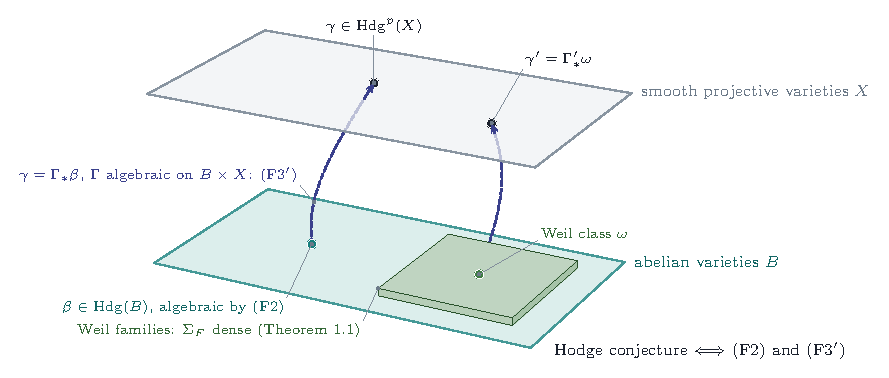
\includegraphics[width=\textwidth]{fig_twohalves}
\caption{The two halves of the conjecture in \Cref{thm:final}(vi). A Hodge
class $\gamma$ on a smooth projective variety $X$ is the image
$\Gamma_{*}\beta$ of a Hodge class $\beta$ on an abelian variety $B$ under an
algebraic correspondence $\Gamma$ on $B\times X$, which is \textup{(F3$'$)};
the class $\beta$ is algebraic, which is \textup{(F2)}, equivalently the
conjecture for abelian varieties (\Cref{prop:f2isab}). The raised plate on
the lower sheet stands for the families of Weil type, on which
\Cref{thm:main} makes the algebraic locus of the Weil class $\omega$ dense;
the dashed part of each correspondence is the part behind the upper sheet.}
\label{fig:twohalves}
\end{figure}


\appendix
\addcontentsline{toc}{part}{\protect\tocpart{}{}{Appendices A to C}}
\section{The exterior algebra model in coordinates}\label{app:exterior}

We record in coordinates the computation behind \Cref{thm:fmtheta}, both to
pin down the sign in \eqref{eq:fmtheta} and because the programs of the
archive \cite{BMB26} use this model.

Let $g\ge1$ and let $W$ be the $\QQ$-vector space with basis
$e_{1},\dots,e_{2g},f_{1},\dots,f_{2g}$. We identify
$V=\langle e_{1},\dots,e_{2g}\rangle$ with $H^{1}(A,\QQ)$ and
$V^{\vee}=\langle f_{1},\dots,f_{2g}\rangle$ with $H^{1}(\Av,\QQ)$, so that
$\bigwedge^{*}W=H^{*}(A\times\Av,\QQ)$.

Number the generators so that the generator numbered $i$ is $e_{i}$ for
$i\le2g$ and $f_{i-2g}$ for $i>2g$. A basis of $\bigwedge^{*}W$ is then
indexed by the subsets $S$ of $\{1,\dots,4g\}$, the basis element $w_{S}$
being the wedge of the generators in $S$ in increasing order. The product
is $w_{S}w_{T}=\varepsilon(S,T)\,w_{S\cup T}$ when $S\cap T=\emptyset$ and zero
otherwise, where
\begin{equation}\label{eq:shufflesign}
  \varepsilon(S,T)=(-1)^{\#\{(s,t)\in S\times T\,:\,s>t\}} .
\end{equation}

The three distinguished elements are
\[
  \ell=\sum_{i=1}^{2g}e_{i}\wedge f_{i},
  \qquad
  \theta=\sum_{j=1}^{g}e_{j}\wedge e_{g+j},
  \qquad
  \theta'=\sum_{j=1}^{g}f_{j}\wedge f_{g+j},
\]
and $p_{*}$ is the linear map $\bigwedge^{*}W\to\bigwedge^{*}V$ that sends
$w_{S}$ to $\varepsilon(S\cap[1,2g],\,S\setminus[1,2g])\,w_{S\cap[1,2g]}$ when
$S\supseteq\{2g+1,\dots,4g\}$ and to zero otherwise.

\begin{lemma}\label{lem:appsign}
Let $0\le k\le g$, let $T\subseteq\{1,\dots,g\}$ with $|T|=k$, let
$U=\{1,\dots,g\}\setminus T$ and $S=U\cup(g+U)$. In the product
$\theta'^{\,k}\cdot e^{\ell}$ the unique term contributing $w_{S}$ after
$p_{*}$ is
\[
  k!\;\Bigl(\prod_{j\in T}f_{j}f_{g+j}\Bigr)\cdot\Bigl(\prod_{i\in S}e_{i}f_{i}\Bigr),
\]
and its image under $p_{*}$ is
$k!\,\sigma(g,k)\,\prod_{j\in U}e_{j}\wedge e_{g+j}$ with
$\sigma(g,k)=(-1)^{g(g+1)/2+k}$, independent of $T$.
\end{lemma}

\begin{proof}
The uniqueness of the term and the identification of $S$ are established in
the proof of \Cref{thm:fmtheta}. The sign is the product of the two shuffle
signs \eqref{eq:shufflesign} relating the displayed word to the target word
$\bigl(\prod_{j\in U}e_{j}e_{g+j}\bigr)\bigl(f_{1}\cdots f_{2g}\bigr)$.
Relabelling the symplectic pairs by a permutation $\pi$ of $\{1,\dots,g\}$
carries the word for $T$ to the word for $\pi(T)$ and multiplies both the
displayed and the target word by the sign of the induced permutation of
generators, so the quotient is unchanged. Since the permutations of
$\{1,\dots,g\}$ act transitively on its $k$-subsets, $\sigma$ depends only on
$(g,k)$. Evaluating at $T=\{1,\dots,k\}$, as in the proof of
\Cref{thm:fmtheta}, gives the stated value.
\end{proof}

\begin{remark}
At $g=2$ the computation can be done by hand. There
$\ell=e_{1}f_{1}+e_{2}f_{2}+e_{3}f_{3}+e_{4}f_{4}$,
$\theta=e_{1}e_{3}+e_{2}e_{4}$ and $\theta'=f_{1}f_{3}+f_{2}f_{4}$, and one
finds $\Phi_{\cP}(1)=-\tfrac12\theta^{2}$, $\Phi_{\cP}(\theta')=\theta$ and
$\Phi_{\cP}(\theta'^{2})=-2$, in agreement with \eqref{eq:fmtheta} for $g=2$,
where $(-1)^{g(g+1)/2}=(-1)^{3}=-1$.
\end{remark}

\section{The locus of Hodge classes}\label{app:cdk}

Deformation arguments about Hodge classes rest on one theorem, that of
Cattani, Deligne and Kaplan \cite{CDK95}: the locus in a family where a given
class stays a Hodge class is an algebraic subvariety, not merely an analytic
one. This appendix states the theorem, proves its elementary part, isolates
the two analytic inputs that the rest requires, computes the example that
matters here, and explains why the theorem is not a route to the Hodge
conjecture. The last point is the one that bears on \Cref{sec:construction},
and it is why the material is set out here rather than cited.

\subsection{Variations of Hodge structure}

\begin{definition}[Variation of Hodge structure]\label{def:vhs}
Let $S$ be a smooth connected complex quasi-projective variety. A
\emph{polarised variation of $\QQ$-Hodge structure} of weight $w$ on $S$
consists of
\begin{enumerate}[label=\textup{(\alph*)},nosep]
\item a local system $\mathbb{V}$ of finite dimensional $\QQ$-vector spaces on
  $S$, with associated holomorphic bundle
  $\cV=\mathbb{V}\otimes_{\QQ}\cO_{S}$ carrying the flat connection $\nabla$
  whose flat sections are $\mathbb{V}$;
\item a decreasing filtration $\cV=F^{0}\supseteq F^{1}\supseteq\cdots$ by
  holomorphic subbundles, inducing on each fibre $\mathbb{V}_{s}$ a
  $\QQ$-Hodge structure of weight $w$;
\item a flat nondegenerate $(-1)^{w}$-symmetric pairing
  $Q\colon\mathbb{V}\otimes\mathbb{V}\to\QQ_{S}$ polarising each fibre;
\end{enumerate}
subject to Griffiths transversality
\begin{equation}\label{eq:transversality}
  \nabla F^{p}\subseteq F^{p-1}\otimes\Omega^{1}_{S}.
\end{equation}
\end{definition}

The example to keep in mind is the geometric one: for $f\colon\cX\to S$ smooth
projective, $\mathbb{V}=R^{w}f_{*}\QQ$ with its Gauss--Manin connection is such
a variation, and \eqref{eq:transversality} is Griffiths' theorem
\cite[Ch.~10]{Voi02}. The other example we use is the Weil family of
\Cref{prop:weildomain} below, which is defined in the first instance by a
period domain rather than by a family of varieties, and which carries a
variation all the same.

\begin{notation}\label{not:totalspace}
Write $\cV^{\mathrm{an}}$ for the total space of $\cV$, a complex manifold
fibred over $S$ with fibre $\mathbb{V}_{s}\otimes\CC$, and
$\mathbb{V}^{\mathrm{tot}}\subset\cV^{\mathrm{an}}$ for the subset of pairs
$(s,\alpha)$ with $\alpha\in\mathbb{V}_{s}$, a covering space of $S$ with
countable fibres.
\end{notation}

\subsection{Hodge loci}

\begin{definition}\label{def:hodgelocus}
Let $\mathbb{V}$ be a polarised variation of weight $2p$ on $S$. Its
\emph{locus of Hodge classes} is
\[
  \Hdg^{p}(\mathbb{V})
  =\bigl\{(s,\alpha)\in\mathbb{V}^{\mathrm{tot}}\;:\;
     \alpha\in F^{p}\cV_{s}\bigr\}.
\]
For $N\in\QQ$ write $\Hdg^{p}_{N}$ for the part with $Q(\alpha,\alpha)=N$.
\end{definition}

By conjugation symmetry, a rational $\alpha$ of weight $2p$ lies in $F^{p}$
exactly when it is of type $(p,p)$. The following two lemmas are elementary,
and they give everything about $\Hdg^{p}$ except algebraicity.

\begin{lemma}[Analyticity]\label{lem:hodgeanalytic}
$\Hdg^{p}(\mathbb{V})$ is a closed analytic subset of
$\mathbb{V}^{\mathrm{tot}}$, and the projection
$\pi\colon\Hdg^{p}(\mathbb{V})\to S$ is locally biholomorphic onto its image on
each connected component. In particular each component is a closed analytic
subvariety of an open subset of $S$, and there are countably many components.
\end{lemma}

\begin{proof}
Work on a simply connected open $U\subseteq S$ over which $\mathbb{V}$ is
trivialised, $\mathbb{V}|_{U}\cong V_{0}\times U$ for a fixed $\QQ$-vector
space $V_{0}$. Then $\mathbb{V}^{\mathrm{tot}}|_{U}$ is the disjoint union over
$\alpha\in V_{0}$ of copies of $U$. Fix $\alpha$. The quotient
$\cV/F^{p}$ is a holomorphic vector bundle on $U$, and the image
$\bar\alpha(s)$ of the flat section $\alpha$ in $(\cV/F^{p})_{s}$ is a
holomorphic section of it. The set of $s\in U$ with $\alpha\in F^{p}\cV_{s}$
is the zero locus of $\bar\alpha$, a closed analytic subset of $U$. Taking
the union over the countable set $V_{0}$ gives the first statement, and shows
that on the sheet indexed by $\alpha$ the projection $\pi$ is the inclusion of
that zero locus into $U$, hence injective. There are countably many
components because $S$ is covered by countably many such $U$, the set $V_{0}$
is countable, and each zero locus has countably many components.
\end{proof}

\begin{lemma}[Finiteness at bounded norm]\label{lem:boundednorm}
Fix $s\in S$ and $N\in\QQ$. The set of $\alpha\in\mathbb{V}_{s}$ with
$\alpha$ of type $(p,p)$, $Q(\alpha,\alpha)=N$, and $\alpha$ in a fixed
lattice $\mathbb{V}_{s,\ZZ}$, is finite. The number of such $\alpha$ is locally
constant on each component of $\Hdg^{p}_{N}$.
\end{lemma}

\begin{proof}
Decompose $\alpha$ into its primitive parts for the Lefschetz decomposition
attached to the polarisation. On the primitive part of type $(p,p)$ in weight
$2p$ the Hodge--Riemann bilinear relations read
$(-1)^{p}\,Q(\alpha,\bbar{\alpha})>0$ for $\alpha\ne0$, so the form
$(-1)^{p}Q$ is positive definite on the real span of the primitive real
$(p,p)$-classes; the same holds on each Lefschetz summand with an alternating
sign, and the resulting form $\tilde Q$ obtained by flipping signs summand by
summand is positive definite on the whole space of real $(p,p)$-classes. The
conditions $Q(\alpha,\alpha)=N$ and $\alpha$ of type $(p,p)$ therefore confine
$\alpha$ to a compact set for $\tilde Q$, and a compact set meets a lattice in
finitely many points. The count is locally constant because the lattice and $Q$
are flat and the Hodge filtration varies continuously, so no Hodge class can
appear or disappear without its $Q$-norm changing.
\end{proof}

\begin{theorem}[Cattani, Deligne and Kaplan \cite{CDK95}]\label{thm:cdk}%
\footnote{The paper is short and the proof is not: the two inputs isolated
below, the nilpotent orbit theorem and the $\SL_{2}$-orbit theorem, carry the
weight.}
Let $S$ be a smooth complex quasi-projective variety and $\mathbb{V}$ a
polarised variation of $\ZZ$-Hodge structure of weight $2p$ on $S$. Then each
connected component of $\Hdg^{p}(\mathbb{V})$ is a closed algebraic subvariety
of $\mathbb{V}^{\mathrm{tot}}$, and its image in $S$ is a closed algebraic
subvariety of $S$.
\end{theorem}

We do not reproduce the proof, which draws on the whole asymptotic theory of
degenerating Hodge structures developed in the two preceding decades. For
families of abelian varieties the algebraicity of these loci also follows, by
a different route, from Deligne's theorem that Hodge classes on abelian
varieties are absolutely Hodge; \Cref{thm:cdk} is what carries it beyond
abelian varieties. We record where the difficulty lies and which two
theorems remove it, since the shape of the argument is what one needs in
order to judge whether a deformation argument in this area is legitimate.

By \Cref{lem:hodgeanalytic} a component $Z$ of $\Hdg^{p}$ is already a closed
analytic subvariety of an open subset of $S$, and by \Cref{lem:boundednorm} it
carries a locally constant $Q$-norm and is one sheet of a finite cover of its
image. Choose a smooth projective compactification $\bar S\supseteq S$ with
$\bar S\setminus S$ a normal crossing divisor. By Chow's theorem it is enough
to show that $Z$ extends to an analytic subvariety of $\bar S$, that is, that
$Z$ does not oscillate wildly as one approaches the boundary. This is an
asymptotic question about the Hodge filtration, and it is answered by two
theorems.

\begin{enumerate}[label=\textup{(\Alph*)},leftmargin=2.2em]
\item \emph{The nilpotent orbit theorem} of Schmid \cite{Sch73}: near a
  boundary point the period map is approximated, to exponentially small error
  in the natural coordinates, by the orbit of a nilpotent Lie algebra element
  built from the local monodromy logarithms.
\item \emph{The $\SL_{2}$-orbit theorem} in several variables, of Cattani,
  Kaplan and Schmid \cite{CKS86}: that nilpotent orbit is in turn approximated
  by an orbit of a fixed real reductive group, with uniform estimates in the
  several-variable setting.
\end{enumerate}

Together these give a two-sided estimate for the Hodge norm of a flat section
near the boundary, of the shape $\|\alpha\|_{s}\sim\prod_{j}(\log|t_{j}|^{-1})^{m_{j}}$
with integers $m_{j}$ determined by the weight filtration. A flat section that
is Hodge on $Z$ has its norm for the positive definite form $\tilde Q$ of
the proof of \Cref{lem:boundednorm} bounded by that lemma, and the
estimate converts that bound into a statement that the possible boundary
behaviours form a finite list. Algebraicity then follows from the analytic
extension across the boundary together with Chow's theorem in $\bar S$.

\begin{remark}\label{rem:cdkinputs}
Both (A) and (B) are theorems about degenerating Hodge structures, and
neither mentions algebraic cycles. The algebraicity in \Cref{thm:cdk} is
algebraicity of a locus of periods, obtained by analysis, and it carries no
information about algebraic cycles; \Cref{ssec:cdknot} develops the point.
\end{remark}

\subsection{The Weil family}

The example relevant to this paper is the family of complex structures on the
model of \Cref{setup:model}.

\begin{proposition}[The Weil period domain]\label{prop:weildomain}
Fix $K$, $n$, the $K$-space $V=K^{2n}$, and the hermitian form $H$ of
signature $(n,n)$ from \Cref{lem:hermform}. The set of Hodge structures of
weight one on $V$ that are polarised by $Q$, commute with the $K$-action, and
are of $(K,-1,n)$-Weil type is in bijection with
\[
  \cD_{n,n}
  =\bigl\{P\subset V_{+}\;:\;\dim_{\CC}P=n,\ H|_{P}\ \text{negative definite}\bigr\},
\]
an open subset of the Grassmannian $\mathrm{Gr}(n,2n)$ and a bounded symmetric
domain isomorphic to $\mathrm{U}(n,n)/\bigl(\mathrm{U}(n)\times\mathrm{U}(n)\bigr)$.
In particular
\[
  \dim_{\CC}\cD_{n,n}=n^{2},
\]
compared with $\dim\cA_{2n}=n(2n+1)$ for the moduli of principally polarised
abelian $2n$-folds.
\end{proposition}

\begin{proof}
A Hodge structure of weight one on $V$ is a subspace $V^{1,0}\subset V_{\CC}$
with $V_{\CC}=V^{1,0}\oplus\overline{V^{1,0}}$. Commuting with the $K$-action
means that $V^{1,0}$ is stable under the operator $S$ of \Cref{setup:model},
so that it splits as $V^{1,0}=P\oplus P'$ with $P=V^{1,0}\cap V_{+}$ and
$P'=V^{1,0}\cap V_{-}$.
Conjugation interchanges $V_{+}$ and $V_{-}$, so
$\overline{V^{1,0}}=\bbar{P}\oplus\bbar{P'}$ with $\bbar{P}\subset V_{-}$, and
the direct sum condition becomes $V_{-}=P'\oplus\bbar{P}$, which determines
$P'$ up to the choice of a complement; the Weil condition
$\dim P=\dim P'=n$ of \Cref{lem:balanced} together with the polarisation
condition pins it down as $P'=\bbar{P}^{\perp_{H}}$. The structure is
therefore determined by $P$.

For the positivity, extend $H$ to the $\CC$-bilinear pairing between $V_{+}$
and $V_{-}$. By the computation \eqref{eq:Qplusminus} in the proof of
\Cref{thm:model}, the second Riemann relation holds exactly when $i\,Q$ is
positive on $V^{1,0}$, and on the $V_{+}$ part this is the condition that $H$
be negative definite on $P$, the sign being fixed by the convention of
\Cref{lem:hermform}. The set of $n$-dimensional negative definite subspaces
of a hermitian space of signature $(n,n)$ is the standard realisation of the
symmetric domain of $\mathrm{U}(n,n)$: the unitary group acts transitively on
it and the stabiliser of a point is $\mathrm{U}(n)\times\mathrm{U}(n)$, the
unitary groups of $P$ and of $P^{\perp}$. It is open in $\mathrm{Gr}(n,2n)$
because negative definiteness is an open condition, and
$\dim\mathrm{Gr}(n,2n)=n(2n-n)=n^{2}$.

For the comparison, $\dim\cA_{g}=g(g+1)/2$, which is $n(2n+1)$ for $g=2n$.
\end{proof}

\begin{corollary}[The Weil locus is algebraic]\label{cor:weilalgebraic}
Inside $\cA_{2n}$ the image of $\cD_{n,n}$, that is the locus of principally
polarised abelian $2n$-folds admitting an action of an order of $K$ of
$(K,-1,n)$-Weil type, is a closed algebraic subvariety of dimension $n^{2}$.
\end{corollary}

\begin{proof}
The condition of admitting such an action is the condition that a certain
class in $\End(H^{1})$, namely the graph of $\iota(\sqrt{-d})$, be a Hodge
class, together with the balanced signature, which is locally constant. The
locus is therefore a component of a locus of Hodge classes for the variation
$\End(R^{1}f_{*}\QQ)$ over $\cA_{2n}$ with its level structure, and
\Cref{thm:cdk} applies. The dimension is \Cref{prop:weildomain}.
\end{proof}

\subsection{Limits of the theorem}\label{ssec:cdknot}

\begin{remark}[Algebraic locus, not algebraic class]\label{rem:notalgebraic}
\Cref{thm:cdk} says that the set of parameters where $\alpha$ is Hodge is cut
out by polynomial equations. It says nothing about whether $\alpha$ is the
class of a cycle at any one of those parameters. The two statements are
independent in both directions: the Hodge locus of a class that happens to be
algebraic everywhere is still known to be algebraic only through
\Cref{thm:cdk}, and conversely the algebraicity of the locus supplies no
cycle. The distinction is easily blurred, and \Cref{cor:weilalgebraic} is
exactly the kind of statement that invites it: the Weil locus is an algebraic
subvariety, even a Shimura subvariety, and none of that produces the class
$\omega_{1}$ of \eqref{eq:omegagens}. \Cref{fig:moduli} compares the
dimension of the Weil locus with that of $\cA_{2n}$.
\end{remark}

\begin{figure}[htbp]
\centering
  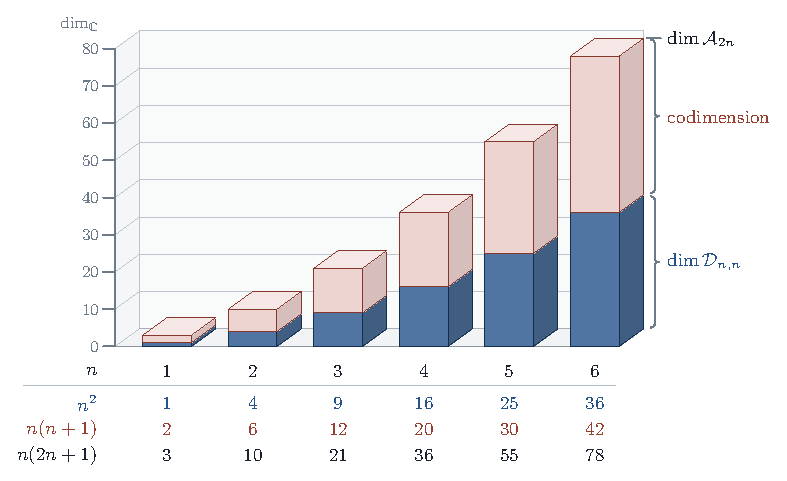
\includegraphics[width=0.92\textwidth]{fig_moduli}
\caption{The Weil locus inside the moduli of principally polarised abelian
$2n$-folds, for $n=1,\dots,6$. Each prism has the height $n(2n+1)$ of the
moduli space $\cA_{2n}$; its lower part, of height $n^{2}$, is the
dimension of the period domain $\cD_{n,n}$ of \Cref{prop:weildomain}, and
its upper part is the codimension $n(n+1)$. The codimension grows
quadratically, so the Weil locus is thin, and by \Cref{cor:weilalgebraic} it
is an algebraic subvariety. Both facts matter for propagation: the locus
along which one would have to deform is small and is a variety, but neither
fact produces a cycle on it.}
\label{fig:moduli}
\end{figure}

\begin{remark}[The variational Hodge conjecture]\label{rem:variational}
The property that would turn \Cref{thm:cdk} into a tool is the variational
Hodge conjecture of Grothendieck: if $\cX\to S$ is smooth projective over a
connected base, $\alpha$ is a flat section of $R^{2p}f_{*}\QQ$ that is Hodge at
every point, and $\alpha_{s_{0}}$ is algebraic at one point $s_{0}$, then
$\alpha_{s}$ is algebraic at every point. Its infinitesimal form is a
theorem under a semiregularity hypothesis: if the cycle at
$s_{0}$ is semiregular in the sense of Bloch \cite{Blo72}, then it deforms to
first order, and hence formally, along the locus where its class stays Hodge.
That theorem is the subject of \Cref{sec:semireg}, and
\Cref{cor:countnotbind} shows that its numerical hypothesis is not what
obstructs the present problem.
\end{remark}

\begin{remark}[The construction of
\texorpdfstring{\Cref{sec:construction}}{Section 14}]\label{rem:cdkconstruction}
The construction of \Cref{sec:construction} produces, for every $n$, every $d$
and every nondegenerate $\beta$, an abelian variety of Weil type together with
secant sheaves whose Chern classes are computed in closed form, and its output
is algebraic on the split locus. The missing ingredient, described in
\Cref{rem:deformation}, is a statement along the algebraic locus of
\Cref{cor:weilalgebraic}: the Hodge type of the deformed object has to be
controlled as the parameter moves off the split locus. \Cref{thm:cdk}
guarantees that the locus along which one deforms is an algebraic variety,
which is what makes the question well posed, but it does not answer the
question. \Cref{q:higher} states it precisely.
\end{remark}

\section{Endomorphism algebras and Weil type}\label{app:albert}

\Cref{def:weiltype} asks for three things: an even dimension, an imaginary
quadratic field acting with balanced eigenvalue multiplicities, and
compatibility with the polarisation. This appendix places these conditions
inside Albert's classification of endomorphism algebras. Two statements used
in the body come out of it. The first is that the compatibility condition is
automatic once the field is stable under the Rosati involution, so that it
reduces to that stability (\Cref{lem:rosatiauto}). The second is that the
balanced condition is not a normalisation but exactly the condition under
which the Weil line carries a Hodge class (\Cref{prop:signatureforced}); this
is why the subject concerns balanced signatures alone.

\subsection{Positive involutions}

\begin{definition}\label{def:positive}
Let $D$ be a finite dimensional semisimple $\QQ$-algebra. An involution
$\dagger$ of $D$, that is a $\QQ$-linear anti-automorphism with
$\dagger^{2}=\id$, is \emph{positive} if
\[
  \Tr_{D/\QQ}\bigl(x\,x^{\dagger}\bigr)>0
  \qquad\text{for every }x\in D,\ x\ne0,
\]
where $\Tr_{D/\QQ}$ is the trace of left multiplication on $D$ as a
$\QQ$-vector space.
\end{definition}

For an abelian variety $A$ with a polarisation $\eta$, the algebra
$D=\End^{0}(A)=\End(A)\otimes\QQ$ is semisimple and the Rosati involution
$\dagger$ attached to $\eta$ is positive \cite[Ch.~5]{BL04}. Everything below
is a statement about the pair $(D,\dagger)$.

\begin{lemma}[Totally real centre]\label{lem:totallyreal}
Let $(D,\dagger)$ be as above with $D$ a division algebra, let $F$ be the
centre of $D$ and $F_{0}=\{z\in F:z^{\dagger}=z\}$. Then $F_{0}$ is a totally
real number field.
\end{lemma}

\begin{proof}
For $z\in F_{0}$ the positivity condition reads
$\Tr_{D/\QQ}(z^{2})>0$, and $\Tr_{D/\QQ}$ restricted to $F_{0}$ is
$[D:F_{0}]\cdot\Tr_{F_{0}/\QQ}$, so $\Tr_{F_{0}/\QQ}(z^{2})>0$ for every
nonzero $z\in F_{0}$. Suppose $F_{0}$ had a complex place $\sigma$. The
embedding of $F_{0}$ into the product of its archimedean completions has dense
image, so there is $z\in F_{0}$ with $\sigma(z)$ within $\tfrac1{10}$ of $i$
and $|\rho(z)|<\varepsilon$ for every other archimedean place $\rho$. Then
$\Tr_{F_{0}/\QQ}(z^{2})=\sum_{\rho}\rho(z)^{2}$, where a complex place
contributes twice the real part of $\rho(z)^{2}$. The real part of
$\sigma(z)^{2}$ is less than $-1+\tfrac{2}{10}+\tfrac{1}{100}<-\tfrac12$, so
the term from $\sigma$ is less than $-1$, and the remaining terms are
bounded in absolute value by $2[F_{0}:\QQ]\varepsilon^{2}$, so the total is
negative for $\varepsilon$ small. This contradicts positivity, so every place
of $F_{0}$ is real.
\end{proof}

\begin{theorem}[Albert \cite{Alb34,Alb35a,Alb35b}]\label{thm:albert}%
\footnote{The numbering of the four types is Albert's and has stuck, although
it follows no natural order: types I to III have a totally real centre and
type IV a CM one, so the natural division is two against two rather than three
against one. Shimura's normalisation of the same classification, in terms of
the associated symmetric domains, is the one that makes the moduli side
transparent.}
Let $(D,\dagger)$ be a division algebra over $\QQ$ with a positive involution,
$F$ its centre, $F_{0}$ the subfield fixed by $\dagger$, $e_{0}=[F_{0}:\QQ]$
and $[D:F]=d^{2}$. Then $F_{0}$ is totally real, $[F:F_{0}]\in\{1,2\}$, and
exactly one of the following holds.
\begin{enumerate}[label=\textup{Type \Roman*.},leftmargin=4.2em,itemsep=2pt]
\item $D=F=F_{0}$ is a totally real field and $\dagger$ is the identity.
\item $F=F_{0}$ is totally real and $D$ is a quaternion algebra over $F$ with
  $D\otimes_{F,\rho}\RR\cong M_{2}(\RR)$ at every real place $\rho$;
  $\dagger$ is of orthogonal type.
\item $F=F_{0}$ is totally real and $D$ is a quaternion algebra over $F$ with
  $D\otimes_{F,\rho}\RR\cong\mathbb{H}$ at every real place $\rho$; $\dagger$
  is the canonical involution.
\item $F$ is a CM field with maximal totally real subfield $F_{0}$, and
  $\dagger$ induces complex conjugation on $F$.
\end{enumerate}
If moreover $D=\End^{0}(A)$ for an abelian variety $A$ of dimension $g$ with
$\dagger$ the Rosati involution of a polarisation, then
\[
  \text{\rm I: } e_{0}\mid g,
  \qquad
  \text{\rm II: } 2e_{0}\mid g,
  \qquad
  \text{\rm III: } 2e_{0}\mid g,
  \qquad
  \text{\rm IV: } e_{0}d^{2}\mid g .
\]
\end{theorem}

We quote \Cref{thm:albert} as a classification. \Cref{lem:totallyreal}
proves the part of it that we use directly, and the four types with their
divisibility conditions are in \cite[Ch.~9]{BL04}. \Cref{fig:albert} draws the
signatures of an imaginary quadratic action and the dimensions of their
families.

\begin{figure}[htbp]
\centering
  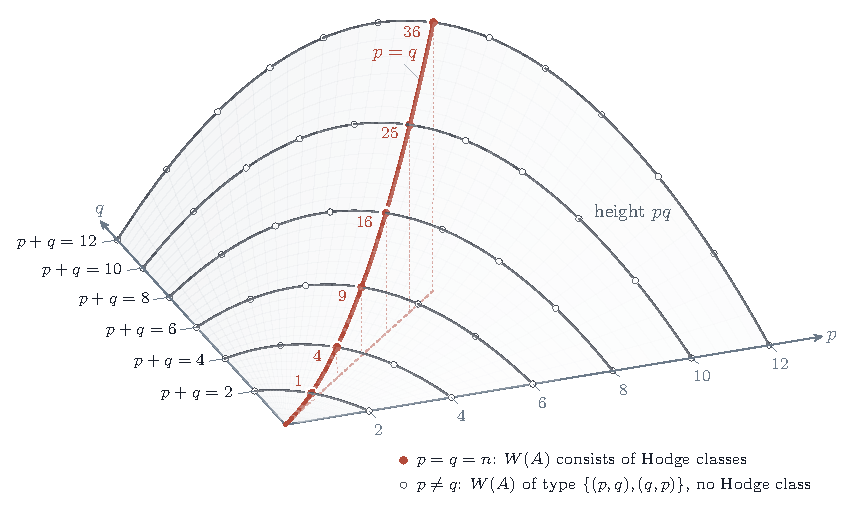
\includegraphics[width=0.92\textwidth]{fig_signature}
\caption{The signatures $(p,q)$ of an imaginary quadratic action, with
$p+q=\dim A$, drawn on the surface of height $pq$, which is the dimension of
the family of abelian varieties carrying that action, the unitary Shimura
variety of signature $(p,q)$. Each curve on the surface collects the
signatures available in one dimension, and on it the diagonal point is the
highest. The divisibility conditions of \Cref{thm:albert} put no
constraint on which of them occur when $\End^{0}(A)=K$, by
\Cref{prop:whichtypes}(i). By \Cref{prop:signatureforced} the Weil line
consists of Hodge classes exactly at the filled points on the ridge
$p=q$, and at every open point it is a rational sub-Hodge structure of type
$\{(p,2n-p),(2n-p,p)\}$ carrying no Hodge class at all. The diagonal is the
locus that \Cref{cor:weilalgebraic} shows to be an algebraic subvariety of the
moduli.}
\label{fig:albert}
\end{figure}

\subsection{Compatibility with the polarisation}

\begin{lemma}[Rosati on an imaginary quadratic subfield]\label{lem:rosatiauto}
Let $A$ be an abelian variety with a polarisation $\eta$ and Rosati involution
$\dagger$, and let $\iota\colon K\hookrightarrow\End^{0}(A)$ be an embedding of
an imaginary quadratic field such that $\iota(K)$ is stable under $\dagger$.
Then
\[
  \iota(\tau)^{\dagger}=\iota(\bbar{\tau})
  \qquad\text{for every }\tau\in K .
\]
That is, condition \textup{(iii)} of \Cref{def:weiltype} holds automatically,
and Weil type is the conjunction of \textup{(i)}, \textup{(ii)} and the
$\dagger$-stability of $\iota(K)$.
\end{lemma}

\begin{proof}
Put $D=\End^{0}(A)$. By stability, $\dagger$ restricts to an involutive
anti-automorphism of the field $\iota(K)\cong K$. An anti-automorphism of a
commutative ring is an automorphism, and $\Gal(K/\QQ)$ has order two, so the
restriction is either the identity or complex conjugation. Suppose it were
the identity, and put $x=\iota(\sqrt{-d})$. Then
$x\,x^{\dagger}=x^{2}=\iota(-d)=-d\cdot 1$, so
\[
  \Tr_{D/\QQ}\bigl(x\,x^{\dagger}\bigr)=-d\cdot\dim_{\QQ}D<0,
\]
contradicting the positivity of $\dagger$. Hence $\dagger$ restricts to complex
conjugation.
\end{proof}

\begin{remark}\label{rem:whystable}
Stability is a real hypothesis: a subfield of $\End^{0}(A)$ need not be
$\dagger$-stable. What \Cref{lem:rosatiauto} removes is the second half of the
condition, the identification of $\dagger|_{K}$ with a specific automorphism.
In particular, in the model of \Cref{setup:model} the polarisation need not be
chosen to match the field, since any $\dagger$-stable embedding does the same
work.
\end{remark}

\subsection{The balanced signature}

\begin{definition}[Signature]\label{def:signature}
Let $\iota\colon K\hookrightarrow\End^{0}(A)$ be as above, $g=\dim A$. The
operator $\iota(\sqrt{-d})$ acts on the tangent space $T_{0}A\cong\CC^{g}$ with
the two eigenvalues $\pm i\sqrt{d}$; write $p$ and $q=g-p$ for their
multiplicities. The pair $(p,q)$ is the \emph{signature} of $(A,\iota)$.
\end{definition}

The signature is an isogeny invariant, since an isogeny induces an isomorphism
on tangent spaces commuting with the action. It is locally constant in
families: the two eigenspaces are the kernels of
$\iota(\sqrt{-d})\mp i\sqrt{d}$ on the relative tangent bundle, so their
dimensions are upper semicontinuous, and they sum to $g$. By
duality $\iota(\tau)^{*}$ acts on $H^{1,0}(A)$ with the same multiplicities, so
$\dim V^{1,0}_{+}=p$ and $\dim V^{1,0}_{-}=q$ in the notation of
\Cref{sec:weiltype}.

\begin{proposition}[The balanced signature is forced]\label{prop:signatureforced}
Let $A$ be an abelian variety of dimension $2n$ with a $\dagger$-stable
embedding $\iota\colon K\hookrightarrow\End^{0}(A)$ of signature $(p,q)$,
$p+q=2n$, and let
\[
  \HW(A)=\Bigl(\textstyle\bigwedge^{2n}_{\CC}V_{+}
   \oplus\bigwedge^{2n}_{\CC}V_{-}\Bigr)\cap H^{2n}(A,\QQ)
\]
as in \Cref{def:weilline}. Then $\HW(A)$ is a rational sub-Hodge structure of
$H^{2n}(A,\QQ)$ of dimension two and of Hodge type
$\{(p,2n-p),\,(2n-p,p)\}$, and the following are equivalent:
\begin{enumerate}[label=\textup{(\roman*)},nosep]
\item $p=q=n$, that is $(A,\iota,\eta)$ is of $(K,-1,n)$-Weil type;
\item $\HW(A)$ contains a nonzero Hodge class;
\item $\HW(A)$ consists of Hodge classes.
\end{enumerate}
\end{proposition}

\begin{proof}
The space $\bigwedge^{2n}V_{+}$ is a line, and by \eqref{eq:bisplit} it equals
$\bigwedge^{p}V^{1,0}_{+}\otimes\bigwedge^{2n-p}V^{0,1}_{+}$, which is of pure
Hodge bidegree $(p,2n-p)$; the conjugate line $\bigwedge^{2n}V_{-}$ is of
bidegree $(2n-p,p)$. Their sum is stable under conjugation and defined over
$\QQ$ by the argument of \Cref{prop:weilline}(i), which does not use the
balanced condition, so $\HW(A)$ is a two-dimensional rational sub-Hodge
structure of the stated type.

A Hodge class is an element of bidegree $(n,n)$. A nonzero element of
$\HW(A)\otimes\CC$ has a nonzero component in one of the two lines, so it is of
bidegree $(n,n)$ only if $(p,2n-p)=(n,n)$ or $(2n-p,p)=(n,n)$, and either
equality says $p=n$. This proves that (ii) implies (i). If $p=n$ then both
lines are of bidegree $(n,n)$ and every element of $\HW(A)$ is a Hodge class,
so (i) implies (iii); and (iii) implies (ii) because $\dim\HW(A)=2>0$.
\end{proof}

\begin{remark}\label{rem:onlybalanced}
\Cref{prop:signatureforced} is the reason the literature speaks of abelian
varieties of Weil type rather than of imaginary quadratic multiplication in
general. For an unbalanced signature the space $\HW(A)$ is still a canonical
two-dimensional rational sub-Hodge structure, and it is still not in the
divisor subring, but it contains no Hodge class and therefore predicts
nothing. The exceptional Hodge classes appear exactly at balance, and the
locus of balance is the algebraic subvariety of \Cref{cor:weilalgebraic}.
\end{remark}

\subsection{Endomorphism algebras of Weil type}

\begin{proposition}[Weil type in the classification]\label{prop:whichtypes}
Let $A$ be an abelian variety of dimension $2n$ admitting a $\dagger$-stable
embedding of an imaginary quadratic field $K$ with balanced signature, and
suppose $\End^{0}(A)$ is a division algebra $D$ with centre $F$ as in
\Cref{thm:albert}. Then:
\begin{enumerate}[label=\textup{(\roman*)},nosep]
\item if $D=K$ then $D$ is of type IV with $e_{0}=1$ and $d=1$, and the
  divisibility condition of \Cref{thm:albert} is vacuous, so every even
  dimension occurs;
\item the classification does not exclude type III with $F_{0}=\QQ$: a
  totally definite quaternion algebra over $\QQ$ contains imaginary
  quadratic subfields on which the canonical involution is conjugation;
\item $D$ is not of type I, because a totally real field contains no
  imaginary quadratic subfield.
\end{enumerate}
\end{proposition}

\begin{proof}
(i) If $D=K$ then $F=K$ is a CM field with $F_{0}=\QQ$, so $e_{0}=1$; and
$[D:F]=1$ gives $d=1$. The involution is conjugation by
\Cref{lem:rosatiauto}, which is type IV. The condition $e_{0}d^{2}\mid g$ reads
$1\mid 2n$.

(ii) Let $D$ be a quaternion algebra over $\QQ$ ramified at the infinite place,
with standard generators $u,v$ satisfying $u^{2}=a<0$, $v^{2}=b<0$, $uv=-vu$,
and canonical involution $x\mapsto\bbar{x}$ fixing $\QQ$ and negating
$u,v,uv$. Then $\QQ(u)\cong\QQ(\sqrt{a})$ is imaginary quadratic, stable under
the involution, and the involution restricts to conjugation on it. Whether
such a $D$ occurs as $\End^{0}(A)$ together with a balanced signature
is a separate question about the moduli, but nothing in the classification
excludes it.

(iii) is immediate, since a totally real field has no element of negative
square.
\end{proof}

\begin{remark}[The generic case]\label{rem:genericcase}
Case (ii) of \Cref{prop:whichtypes} is a special position: there
$\End^{0}(A)$ is larger than $K$, the Hodge group is correspondingly smaller,
and $\Hdg^{n}(A)$ can be larger than the three dimensions of
\Cref{thm:hdgcount}. It is also a case in which the Weil classes can become
accessible: \Cref{rem:special} records that at such points the Weil line can
meet the divisor subring, which is the split situation. The hard case, and the
one addressed throughout \Cref{sec:divisor,sec:characters,sec:hyperplane}, is
case (i) with $\Hg(A)=\SU(V,H)$.
\end{remark}

\begin{remark}[Dimension four]\label{rem:dimfour}
For $n=1$ the Weil line lies in $H^{2}(A,\QQ)$ and consists of divisor
classes, algebraic by the Lefschetz theorem on $(1,1)$ classes, so it predicts
nothing new; this is the same boundary as in \Cref{prop:normpart}. Moonen and
Zarhin determined the Hodge classes on abelian varieties of dimension at most
five \cite{MZ99}, and on simple abelian fourfolds in \cite{MZ95}: through
dimension three the Hodge ring is generated by divisor classes, and the first
Hodge classes not of that form occur in dimension four, on abelian fourfolds of
Weil type. Thus $n=2$ is at once the first case of \Cref{def:weiltype} with
exceptional Hodge classes, the first case where \Cref{thm:hdgcount} gives
three rather than one, and the first case of the Hodge conjecture for
abelian varieties that needed more than divisor classes; Markman settled it
\cite[Corollary 1.6.1]{Mar25a}. The next case is $n=3$ with nontrivial
discriminant, by \Cref{prop:separate}(ii).
\end{remark}


\addcontentsline{toc}{part}{\protect\tocpart{}{}{Declarations and references}}
% \zenodoCodeID is the one DOI the paper cites for the code, in the data
% availability section and in the entry BMB26 of the bibliography: the version
% DOI of release v5.0.1. Releases v1.0.0, v2.0.0, v3.0.0, v3.1.1, v3.2.0,
% v4.0.0 and v5.0.0 are 10.5281/zenodo.22950276, 10.5281/zenodo.23038895,
% 10.5281/zenodo.23047883, 10.5281/zenodo.23078541, 10.5281/zenodo.23093099,
% 10.5281/zenodo.23197107 and 10.5281/zenodo.23221435; all are versions of the
% concept record 10.5281/zenodo.22950275.
\newcommand{\zenodoCodeID}{10.5281/zenodo.23225483}
\newcommand{\zenodoCodeDOI}{%
  \href{https://doi.org/\zenodoCodeID}{\texttt{\zenodoCodeID}}}

\section*{Declarations}

\subsection*{Funding}
The authors received no funding for this work.

\subsection*{Competing interests}
The authors have no competing interests to declare.

\subsection*{Ethics approval and consent}
This article reports no research involving human participants, human data or
animals, so ethics approval and consent to participate or to publish were not
required. The results are original and have not been published elsewhere,
and the work of others is credited by citation throughout.

\subsection*{Data availability}
The programs of the archive \cite{BMB26}, which repeat much of the finite
arithmetic of the proofs as an independent check, the Lean~4 certificate of
part of that arithmetic, the Macaulay2
computations of local $\Ext$ algebras with their output, the sources of the
paper, and the generators and TikZ sources of every figure are openly
available on Zenodo under the DOI \zenodoCodeDOI; the version that
accompanies this paper is release 5.0.1 of the archive. A document in the
archive lists, for each result of the paper, the computations that check
it. The programs perform $2218$ checks, all of which pass, and the
Lean kernel checks four hundred and nine theorems, each depending on no axiom
or on propositional extensionality alone. Deep Bhattacharjee computed all
the calculations, in C, Python, Julia, Macaulay2, Lean~4 and shell scripts,
with the assistance of Claude Code, an AI model developed by Anthropic. The
programs in the archive are those in Python, which use the C libraries FLINT
and Arb through python-flint, in Macaulay2 and in shell scripts, together
with the Lean~4 certificate, in which he formalised the finite arithmetic.
Every result they certify can be reproduced from the archive
with the programs and the Lean kernel, and the authors are responsible for
the mathematical statements and their proofs. No other data were generated
or analysed.


\begin{thebibliography}{99}

\bibitem[ABLP26]{ABLP26}
H. Awada, M. Bolognesi, R. Laterveer and C. Pedrini,
\emph{K3 surfaces and cubic fourfolds with Abelian motive},
Ann. Mat. Pura Appl. (4), published online 2026; arXiv:2012.05969.
\href{https://doi.org/10.1007/s10231-026-01689-x}{\texttt{doi:10.1007/s10231-026-01689-x}}.

\bibitem[ACa79]{ACa79}
N. A'Campo,
\emph{Tresses, monodromie et le groupe symplectique},
Comment. Math. Helv. \textbf{54} (1979), 318--327.
\href{https://doi.org/10.1007/BF02566275}{\texttt{doi:10.1007/BF02566275}}.

\bibitem[ACGH85]{ACGH85}
E. Arbarello, M. Cornalba, P. A. Griffiths and J. Harris,
\emph{Geometry of Algebraic Curves, Volume I},
Grundlehren der Mathematischen Wissenschaften \textbf{267},
Springer, New York, 1985.

\bibitem[Alb34]{Alb34}
A. A. Albert,
\emph{On the construction of Riemann matrices. I},
Ann. of Math. (2) \textbf{35} (1934), no.~1, 1--28.
\href{https://doi.org/10.2307/1968116}{\texttt{doi:10.2307/1968116}}.

\bibitem[Alb35a]{Alb35a}
A. A. Albert,
\emph{On the construction of Riemann matrices. II},
Ann. of Math. (2) \textbf{36} (1935), no.~2, 376--394.
\href{https://doi.org/10.2307/1968578}{\texttt{doi:10.2307/1968578}}.

\bibitem[Alb35b]{Alb35b}
A. A. Albert,
\emph{Involutorial simple algebras and real Riemann matrices},
Ann. of Math. (2) \textbf{36} (1935), no.~4, 886--964.
\href{https://doi.org/10.2307/1968595}{\texttt{doi:10.2307/1968595}}.

\bibitem[Ale97]{Ale97}
H. Alexander,
\emph{Holomorphic chains and the support hypothesis conjecture},
J. Amer. Math. Soc. \textbf{10} (1997), no.~1, 123--138.
\href{https://doi.org/10.1090/S0894-0347-97-00218-X}{\texttt{doi:10.1090/S0894-0347-97-00218-X}}.

\bibitem[And92]{And92}
Y. Andr\'e,
\emph{Mumford--Tate groups of mixed Hodge structures and the theorem of the
fixed part},
Compositio Math. \textbf{82} (1992), no.~1, 1--24.
\href{http://www.numdam.org/item/CM_1992__82_1_1_0/}{\texttt{numdam.org/item/CM\_1992\_\_82\_1\_1\_0}}.

\bibitem[And96a]{And96}
Y. Andr\'e,
\emph{On the Shafarevich and Tate conjectures for hyperk\"ahler varieties},
Math. Ann. \textbf{305} (1996), no.~1, 205--248.
\href{https://doi.org/10.1007/BF01444219}{\texttt{doi:10.1007/BF01444219}}.

\bibitem[And96b]{And96b}
Y. Andr\'e,
\emph{Pour une th\'eorie inconditionnelle des motifs},
Inst. Hautes \'Etudes Sci. Publ. Math. \textbf{83} (1996), 5--49.
\href{https://doi.org/10.1007/BF02698643}{\texttt{doi:10.1007/BF02698643}}.

\bibitem[AP07]{AP07}
J. D. Achter and R. Pries,
\emph{The integral monodromy of hyperelliptic and trielliptic curves},
Math. Ann. \textbf{338} (2007), no.~1, 187--206; arXiv:math/0608038.
\href{https://doi.org/10.1007/s00208-006-0072-0}{\texttt{doi:10.1007/s00208-006-0072-0}}.

\bibitem[BB66]{BB66}
W. L. Baily, Jr. and A. Borel,
\emph{Compactification of arithmetic quotients of bounded symmetric domains},
Ann. of Math. (2) \textbf{84} (1966), no.~3, 442--528.
\href{https://doi.org/10.2307/1970457}{\texttt{doi:10.2307/1970457}}.

\bibitem[BD85]{BD85}
A. Beauville and R. Donagi,
\emph{La vari\'et\'e des droites d'une hypersurface cubique de dimension
$4$},
C. R. Acad. Sci. Paris S\'er. I Math. \textbf{301} (1985), no.~14, 703--706.

\bibitem[Bea83]{Bea83}
A. Beauville,
\emph{Vari\'et\'es K\"ahleriennes dont la premi\`ere classe de Chern est
nulle},
J. Differential Geom. \textbf{18} (1983), no.~4, 755--782.
\href{https://doi.org/10.4310/jdg/1214438181}{\texttt{doi:10.4310/jdg/1214438181}}.

\bibitem[BF03]{BF03}
R.-O. Buchweitz and H. Flenner,
\emph{A semiregularity map for modules and applications to deformations},
Compositio Math. \textbf{137} (2003), no.~2, 135--210.
\href{https://doi.org/10.1023/A:1023999012081}{\texttt{doi:10.1023/A:1023999012081}}.

\bibitem[BF08]{BF08}
R.-O. Buchweitz and H. Flenner,
\emph{The global decomposition theorem for Hochschild (co-)homology of
singular spaces via the Atiyah--Chern character},
Adv. Math. \textbf{217} (2008), no.~1, 243--281.
\href{https://doi.org/10.1016/j.aim.2007.06.013}{\texttt{doi:10.1016/j.aim.2007.06.013}}.

\bibitem[BL24]{BL24}
M. Bolognesi and R. Laterveer,
\emph{A $9$-dimensional family of K3 surfaces with finite-dimensional motive},
Rend. Circ. Mat. Palermo (2) \textbf{73} (2024), 2313--2331.
\href{https://doi.org/10.1007/s12215-024-01036-0}{\texttt{doi:10.1007/s12215-024-01036-0}}.

\bibitem[BLM23]{BLM23}
R. Bandiera, E. Lepri and M. Manetti,
\emph{$L_{\infty}$ liftings of semiregularity maps via Chern--Simons classes},
Adv. Math. \textbf{435} (2023), 109358; arXiv:2111.12985.
\href{https://doi.org/10.1016/j.aim.2023.109358}{\texttt{doi:10.1016/j.aim.2023.109358}}.

\bibitem[BMB26]{BMB26}
D. Bhattacharjee, P. Mandal and U. Bhattacharya,
\emph{Verification code and figure sources for the paper ``Algebraic Loci of
Weil Classes on Abelian Varieties''}, software archive with a Lean~4
certificate, release 5.0.1, Zenodo, 2026.
\href{https://doi.org/\zenodoCodeID}{\texttt{doi:\zenodoCodeID}}.

\bibitem[BHPV04]{BHPV04}
W. P. Barth, K. Hulek, C. A. M. Peters and A. Van de Ven,
\emph{Compact Complex Surfaces}, 2nd ed.,
Ergebnisse der Mathematik und ihrer Grenzgebiete, 3. Folge, \textbf{4},
Springer, Berlin, 2004.
\href{https://doi.org/10.1007/978-3-642-57739-0}{\texttt{doi:10.1007/978-3-642-57739-0}}.

\bibitem[BL04]{BL04}
C. Birkenhake and H. Lange,
\emph{Complex Abelian Varieties}, 2nd ed.,
Grundlehren der mathematischen Wissenschaften \textbf{302},
Springer, Berlin, 2004.
\href{https://doi.org/10.1007/978-3-662-06307-1}{\texttt{doi:10.1007/978-3-662-06307-1}}.

\bibitem[BEK14]{BEK14}
S. Bloch, H. Esnault and M. Kerz,
\emph{$p$-adic deformation of algebraic cycle classes},
Invent. Math. \textbf{195} (2014), 673--722.
\href{https://doi.org/10.1007/s00222-013-0461-4}{\texttt{doi:10.1007/s00222-013-0461-4}}.

\bibitem[Bor60]{Bor60}
A. Borel,
\emph{Density properties for certain subgroups of semi-simple groups without
compact components},
Ann. of Math. (2) \textbf{72} (1960), 179--188.
\href{https://doi.org/10.2307/1970150}{\texttt{doi:10.2307/1970150}}.

\bibitem[Bry87]{Bry87}
R. L. Bryant,
\emph{Metrics with exceptional holonomy},
Ann. of Math. (2) \textbf{126} (1987), no.~3, 525--576.

\bibitem[BS83]{BS83}
S. Bloch and V. Srinivas,
\emph{Remarks on correspondences and algebraic cycles},
Amer. J. Math. \textbf{105} (1983), no.~5, 1235--1253.
\href{https://doi.org/10.2307/2374341}{\texttt{doi:10.2307/2374341}}.

\bibitem[BS94]{BS94}
S. Bando and Y.-T. Siu,
\emph{Stable sheaves and Einstein--Hermitian metrics},
in: Geometry and Analysis on Complex Manifolds,
World Sci. Publ., River Edge, NJ, 1994, pp.~39--50.
\href{https://doi.org/10.1142/9789814350112_0002}{\texttt{doi:10.1142/9789814350112\_0002}}.

\bibitem[Blo72]{Blo72}
S. Bloch,
\emph{Semi-regularity and de Rham cohomology},
Invent. Math. \textbf{17} (1972), 51--66.
\href{https://doi.org/10.1007/BF01390023}{\texttt{doi:10.1007/BF01390023}}.

\bibitem[B\"ul20]{Bue20}
T.-H. B\"ulles,
\emph{Motives of moduli spaces on K3 surfaces and of special cubic
fourfolds},
Manuscripta Math. \textbf{161} (2020), 109--124; arXiv:1806.08284.
\href{https://doi.org/10.1007/s00229-018-1086-0}{\texttt{doi:10.1007/s00229-018-1086-0}}.

\bibitem[Bus19]{Bus19}
N. Buskin,
\emph{Every rational Hodge isometry between two K3 surfaces is algebraic},
J. Reine Angew. Math. \textbf{755} (2019), 127--150.
\href{https://doi.org/10.1515/crelle-2017-0027}{\texttt{doi:10.1515/crelle-2017-0027}}.

\bibitem[Cal05]{Cal05}
A. C\u{a}ld\u{a}raru,
\emph{The Mukai pairing, II: the Hochschild--Kostant--Rosenberg isomorphism},
Adv. Math. \textbf{194} (2005), no.~1, 34--66.
\href{https://doi.org/10.1016/j.aim.2004.05.012}{\texttt{doi:10.1016/j.aim.2004.05.012}}.

\bibitem[Cam92]{Cam92}
F. Campana,
\emph{Connexit\'e rationnelle des vari\'et\'es de Fano},
Ann. Sci. \'Ecole Norm. Sup. (4) \textbf{25} (1992), no.~5, 539--545.
\href{https://doi.org/10.24033/asens.1658}{\texttt{doi:10.24033/asens.1658}}.

\bibitem[CDK95]{CDK95}
E. Cattani, P. Deligne and A. Kaplan,
\emph{On the locus of Hodge classes},
J. Amer. Math. Soc. \textbf{8} (1995), no.~2, 483--506.
\href{https://doi.org/10.1090/S0894-0347-1995-1273413-2}{\texttt{doi:10.1090/S0894-0347-1995-1273413-2}}.

\bibitem[CKS86]{CKS86}
E. Cattani, A. Kaplan and W. Schmid,
\emph{Degeneration of Hodge structures},
Ann. of Math. (2) \textbf{123} (1986), no.~3, 457--535.
\href{https://doi.org/10.2307/1971333}{\texttt{doi:10.2307/1971333}}.

\bibitem[CLS11]{CLS11}
D. A. Cox, J. B. Little and H. K. Schenck,
\emph{Toric Varieties},
Grad. Stud. Math. \textbf{124}, Amer. Math. Soc., Providence, RI, 2011.
\href{https://doi.org/10.1090/gsm/124}{\texttt{doi:10.1090/gsm/124}}.

\bibitem[CM13]{CM13}
F. Charles and E. Markman,
\emph{The standard conjectures for holomorphic symplectic varieties
deformation equivalent to Hilbert schemes of K3 surfaces},
Compos. Math. \textbf{149} (2013), no.~3, 481--494.
\href{https://doi.org/10.1112/S0010437X12000607}{\texttt{doi:10.1112/S0010437X12000607}}.

\bibitem[CM78]{CM78}
A. Conte and J. P. Murre,
\emph{The Hodge conjecture for fourfolds admitting a covering by rational
curves},
Math. Ann. \textbf{238} (1978), 79--88.
\href{https://doi.org/10.1007/BF01351457}{\texttt{doi:10.1007/BF01351457}}.

\bibitem[CRV12]{CRV12}
D. Calaque, C. A. Rossi and M. Van den Bergh,
\emph{C\u{a}ld\u{a}raru's conjecture and Tsygan's formality},
Ann. of Math. (2) \textbf{176} (2012), no.~2, 865--923.
\href{https://doi.org/10.4007/annals.2012.176.2.4}{\texttt{doi:10.4007/annals.2012.176.2.4}}.

\bibitem[dCM02]{dCM02}
M. A. de Cataldo and L. Migliorini,
\emph{The Chow groups and the motive of the Hilbert scheme of points on a
surface},
J. Algebra \textbf{251} (2002), no.~2, 824--848.
\href{https://doi.org/10.1006/jabr.2001.9105}{\texttt{doi:10.1006/jabr.2001.9105}}.

\bibitem[Del71]{Del71}
P. Deligne,
\emph{Th\'eorie de Hodge. II},
Inst. Hautes \'Etudes Sci. Publ. Math. \textbf{40} (1971), 5--57.
\href{https://doi.org/10.1007/BF02684692}{\texttt{doi:10.1007/BF02684692}}.

\bibitem[Del72]{Del72}
P. Deligne,
\emph{La conjecture de Weil pour les surfaces $K3$},
Invent. Math. \textbf{15} (1972), 206--226.
\href{https://doi.org/10.1007/BF01404126}{\texttt{doi:10.1007/BF01404126}}.

\bibitem[Del74]{Del74}
P. Deligne,
\emph{La conjecture de Weil. I},
Inst. Hautes \'Etudes Sci. Publ. Math. \textbf{43} (1974), 273--307.
\href{https://doi.org/10.1007/BF02684373}{\texttt{doi:10.1007/BF02684373}}.

\bibitem[Del82]{Del82}
P. Deligne,
\emph{Hodge cycles on abelian varieties} (notes by J. S. Milne),
in: Hodge Cycles, Motives, and Shimura Varieties,
Lecture Notes in Math. \textbf{900}, Springer, Berlin, 1982, pp.~9--100.
\href{https://doi.org/10.1007/978-3-540-38955-2_3}%
{\texttt{doi:10.1007/978-3-540-38955-2\_3}}.

\bibitem[Dem82]{Dem82}
J.-P. Demailly,
\emph{Courants positifs extr\^emaux et conjecture de Hodge},
Invent. Math. \textbf{69} (1982), no.~3, 347--374.
\href{https://doi.org/10.1007/BF01389359}{\texttt{doi:10.1007/BF01389359}}.

\bibitem[Dem12]{Dem12}
J.-P. Demailly,
\emph{Complex Analytic and Differential Geometry},
OpenContent book, Institut Fourier, Grenoble, 2012,
\href{https://www-fourier.univ-grenoble-alpes.fr/~demailly/manuscripts/agbook.pdf}{\texttt{www-fourier.univ-grenoble-alpes.fr/\~{}demailly/manuscripts/agbook.pdf}}.

\bibitem[DM82]{DM82}
P. Deligne and J. S. Milne,
\emph{Tannakian categories},
in: Hodge Cycles, Motives, and Shimura Varieties,
Lecture Notes in Math. \textbf{900}, Springer, Berlin, 1982, pp.~101--228.
\href{https://doi.org/10.1007/978-3-540-38955-2_4}%
{\texttt{doi:10.1007/978-3-540-38955-2\_4}}.

\bibitem[DM86]{DM86}
P. Deligne and G. D. Mostow,
\emph{Monodromy of hypergeometric functions and non-lattice integral
monodromy},
Inst. Hautes \'Etudes Sci. Publ. Math. \textbf{63} (1986), 5--89.

\bibitem[EGL01]{EGL01}
G. Ellingsrud, L. G\"ottsche and M. Lehn,
\emph{On the cobordism class of the Hilbert scheme of a surface},
J. Algebraic Geom. \textbf{10} (2001), no.~1, 81--100.

\bibitem[Fed69]{Fed69}
H. Federer,
\emph{Geometric Measure Theory},
Grundlehren der mathematischen Wissenschaften \textbf{153},
Springer, Berlin, 1969.

\bibitem[Fed74]{Fed74}
H. Federer,
\emph{Real flat chains, cochains and variational problems},
Indiana Univ. Math. J. \textbf{24} (1974/75), no.~4, 351--407.
\href{https://doi.org/10.1512/iumj.1975.24.24031}{\texttt{doi:10.1512/iumj.1975.24.24031}}.

\bibitem[FF60]{FF60}
H. Federer and W. H. Fleming,
\emph{Normal and integral currents},
Ann. of Math. (2) \textbf{72} (1960), no.~3, 458--520.
\href{https://doi.org/10.2307/1970227}{\texttt{doi:10.2307/1970227}}.

\bibitem[FFZ21]{FFZ21}
S. Floccari, L. Fu and Z. Zhang,
\emph{On the motive of O'Grady's ten-dimensional hyper-K\"ahler varieties},
Commun. Contemp. Math. \textbf{23} (2021), no.~4, paper no.~2050034,
50~pp.
\href{https://doi.org/10.1142/S0219199720500340}{\texttt{doi:10.1142/S0219199720500340}}.

\bibitem[FK26]{FK26}
D. Favero and T. L. Kelly,
\emph{The Chern character of a coherent sheaf on a smooth projective
hypersurface},
preprint, 2026.
\href{https://arxiv.org/abs/2609.12759}{\texttt{arXiv:2609.12759}}.

\bibitem[Flo23]{Flo23}
S. Floccari,
\emph{On the motive of O'Grady's six-dimensional hyper-K\"ahler varieties},
\'Epijournal G\'eom. Alg\'ebrique \textbf{7} (2023), Article no.~4;
arXiv:2203.16257.
\href{https://doi.org/10.46298/epiga.2022.9758}{\texttt{doi:10.46298/epiga.2022.9758}}.

\bibitem[Flo25]{Flo25}
S. Floccari,
\emph{K3 surfaces associated with varieties of generalized Kummer type},
Geom. Topol. \textbf{30} (2026), no.~3, 1129--1154; arXiv:2501.02315.
\href{https://doi.org/10.2140/gt.2026.30.1129}{\texttt{doi:10.2140/gt.2026.30.1129}}.

\bibitem[FM98]{FM98}
B. Fantechi and M. Manetti,
\emph{Obstruction calculus for functors of Artin rings, I},
J. Algebra \textbf{202} (1998), no.~2, 541--576.
\href{https://doi.org/10.1006/jabr.1997.7239}{\texttt{doi:10.1006/jabr.1997.7239}}.

\bibitem[FF26]{FF26}
S. Floccari and L. Fu,
\emph{The Hodge conjecture for Weil fourfolds with discriminant $1$ via
singular OG6-varieties},
J. Math. Pures Appl. (9) \textbf{210} (2026), paper no.~103876.
\href{https://doi.org/10.1016/j.matpur.2026.103876}{\texttt{doi:10.1016/j.matpur.2026.103876}}.

\bibitem[Flo24]{Flo24}
S. Floccari,
\emph{Sixfolds of generalized Kummer type and K3 surfaces},
Compos. Math. \textbf{160} (2024), no.~2, 388--410.
\href{https://doi.org/10.1112/S0010437X23007625}{\texttt{doi:10.1112/S0010437X23007625}}.

\bibitem[Fox53]{Fox53}
R. H. Fox,
\emph{Free differential calculus. I. Derivation in the free group ring},
Ann. of Math. (2) \textbf{57} (1953), no.~3, 547--560.

\bibitem[FTV19]{FTV19}
L. Fu, Z. Tian and C. Vial,
\emph{Motivic hyper-K\"ahler resolution conjecture, I: generalized Kummer
varieties},
Geom. Topol. \textbf{23} (2019), no.~1, 427--492; arXiv:1608.04968.
\href{https://doi.org/10.2140/gt.2019.23.427}{\texttt{doi:10.2140/gt.2019.23.427}}.

\bibitem[Fuj87]{Fuj87}
A. Fujiki,
\emph{On the de Rham cohomology group of a compact K\"ahler symplectic
manifold},
in: Algebraic Geometry, Sendai, 1985, Adv. Stud. Pure Math. \textbf{10}
(1987), 105--165.
\href{https://doi.org/10.2969/aspm/01010105}{\texttt{doi:10.2969/aspm/01010105}}.

\bibitem[Ful98]{Ful98}
W. Fulton,
\emph{Intersection Theory}, 2nd ed.,
Ergebnisse der Mathematik und ihrer Grenzgebiete (3) \textbf{2},
Springer, New York, 1998.
\href{https://doi.org/10.1007/978-1-4612-1700-8}{\texttt{doi:10.1007/978-1-4612-1700-8}}.

\bibitem[FH91]{FH91}
W. Fulton and J. Harris,
\emph{Representation Theory: A First Course},
Graduate Texts in Mathematics \textbf{129}, Springer, New York, 1991.

\bibitem[FV25]{FV25}
S. Floccari and M. Varesco,
\emph{Algebraic cycles on hyper-K\"ahler varieties of generalized Kummer
type},
Math. Ann. \textbf{391} (2025), 4443--4453; arXiv:2308.04865.
\href{https://doi.org/10.1007/s00208-024-03027-z}{\texttt{doi:10.1007/s00208-024-03027-z}}.

\bibitem[Gal00]{Gal00}
F. Galluzzi,
\emph{Abelian fourfold of Mumford-type and Kuga--Satake varieties},
Indag. Math. (N.S.) \textbf{11} (2000), no.~4, 547--560.
\href{https://doi.org/10.1016/S0019-3577(00)80024-5}{\texttt{doi:10.1016/S0019-3577(00)80024-5}}.

\bibitem[GDHL09]{GDHL09}
G. Gonz\'alez-Diez, R. A. Hidalgo and M. Leyton,
\emph{Generalized Fermat curves},
J. Algebra \textbf{321} (2009), no.~6, 1643--1660.

\bibitem[GH78]{GH78}
P. Griffiths and J. Harris,
\emph{Principles of Algebraic Geometry},
Wiley, New York, 1978.

\bibitem[GM88]{GM88}
W. M. Goldman and J. J. Millson,
\emph{The deformation theory of representations of fundamental groups of
compact K\"ahler manifolds},
Inst. Hautes \'Etudes Sci. Publ. Math. \textbf{67} (1988), 43--96.
\href{https://doi.org/10.1007/BF02699127}{\texttt{doi:10.1007/BF02699127}}.

\bibitem[GP98]{GP98}
M. Gross and S. Popescu,
\emph{Equations of $(1,d)$-polarized abelian surfaces},
Math. Ann. \textbf{310} (1998), no.~2, 333--377.
\href{https://doi.org/10.1007/s002080050151}{\texttt{doi:10.1007/s002080050151}}.

\bibitem[Gri10]{Gri10}
J. Grivaux,
\emph{Chern classes in Deligne cohomology for coherent analytic sheaves},
Math. Ann. \textbf{347} (2010), no.~2, 249--284.
\href{https://doi.org/10.1007/s00208-009-0430-9}{\texttt{doi:10.1007/s00208-009-0430-9}}.

\bibitem[Gro61]{Gro61}
A. Grothendieck,
\emph{Techniques de construction et th\'eor\`emes d'existence en g\'eom\'etrie
alg\'ebrique IV: les sch\'emas de Hilbert},
S\'eminaire Bourbaki, Vol.~6 (1960/61), Exp. No.~221, 249--276;
reprinted by Soc. Math. France, Paris, 1995.

\bibitem[GW09]{GW09}
R. Goodman and N. R. Wallach,
\emph{Symmetry, Representations, and Invariants},
Graduate Texts in Mathematics \textbf{255}, Springer, New York, 2009.
\href{https://doi.org/10.1007/978-0-387-79852-3}{\texttt{doi:10.1007/978-0-387-79852-3}}.

\bibitem[Har77]{Har77}
R. Hartshorne,
\emph{Algebraic geometry},
Grad. Texts in Math. \textbf{52}, Springer, New York, 1977.
\href{https://doi.org/10.1007/978-1-4757-3849-0}{\texttt{doi:10.1007/978-1-4757-3849-0}}.

\bibitem[Hir64]{Hir64}
H. Hironaka,
\emph{Resolution of singularities of an algebraic variety over a field of
characteristic zero. I, II},
Ann. of Math. (2) \textbf{79} (1964), no.~1, 109--203; no.~2, 205--326.
\href{https://doi.org/10.2307/1970486}{\texttt{doi:10.2307/1970486}},
\href{https://doi.org/10.2307/1970547}{\texttt{doi:10.2307/1970547}}.

\bibitem[HK74]{HK74}
F. R. Harvey and A. W. Knapp,
\emph{Positive $(p,p)$-forms, Wirtinger's inequality and currents},
in: Value-Distribution Theory, Part A (Tulane Univ., 1972--73),
Dekker, New York, 1974, pp.~43--62.

\bibitem[HL82]{HL82}
R. Harvey and H. B. Lawson, Jr.,
\emph{Calibrated geometries},
Acta Math. \textbf{148} (1982), 47--157.
\href{https://doi.org/10.1007/BF02392726}{\texttt{doi:10.1007/BF02392726}}.

\bibitem[HS74]{HS74}
R. Harvey and B. Shiffman,
\emph{A characterization of holomorphic chains},
Ann. of Math. (2) \textbf{99} (1974), no.~3, 553--587.
\href{https://doi.org/10.2307/1971062}{\texttt{doi:10.2307/1971062}}.

\bibitem[HL09]{HL09}
F. R. Harvey and H. B. Lawson, Jr.,
\emph{Duality of positive currents and plurisubharmonic functions in
calibrated geometry},
Amer. J. Math. \textbf{131} (2009), no.~5, 1211--1240.
\href{https://arxiv.org/abs/0710.3921}{\texttt{arXiv:0710.3921}}.

\bibitem[HM73]{HM73}
G. Horrocks and D. Mumford,
\emph{A rank $2$ vector bundle on $\mathbf{P}^{4}$ with $15{,}000$ symmetries},
Topology \textbf{12} (1973), 63--81.
\href{https://doi.org/10.1016/0040-9383(73)90022-0}{\texttt{doi:10.1016/0040-9383(73)90022-0}}.

\bibitem[Hua21]{Hua21}
S. Huang,
\emph{A note on a question of Markman},
J. Pure Appl. Algebra \textbf{225} (2021), no.~9, 106673.
\href{https://doi.org/10.1016/j.jpaa.2021.106673}{\texttt{doi:10.1016/j.jpaa.2021.106673}}.

\bibitem[Huy16]{Huy16}
D. Huybrechts,
\emph{Lectures on K3 Surfaces},
Cambridge Studies in Advanced Mathematics \textbf{158},
Cambridge University Press, Cambridge, 2016.
\href{https://doi.org/10.1017/CBO9781316594193}{\texttt{doi:10.1017/CBO9781316594193}}.

\bibitem[ILP22]{ILP22}
C. Ingalls, A. Logan and O. Patashnick,
\emph{Explicit coverings of families of elliptic surfaces by squares of
curves},
Math. Z. \textbf{302} (2022), 1191--1238; arXiv:2009.07807.
\href{https://doi.org/10.1007/s00209-022-03090-9}{\texttt{doi:10.1007/s00209-022-03090-9}}.

\bibitem[Jan92]{Jan92}
U. Jannsen,
\emph{Motives, numerical equivalence, and semi-simplicity},
Invent. Math. \textbf{107} (1992), no.~3, 447--452.
\href{https://doi.org/10.1007/BF01231898}{\texttt{doi:10.1007/BF01231898}}.

\bibitem[Jum26]{Jum26}
R. Jumagulov,
\emph{The Hodge conjecture for Fermat fourfolds of odd degree at most
$199$},
preprint, 2026.
\href{https://arxiv.org/abs/2608.18134}{\texttt{arXiv:2608.18134}}.

\bibitem[Kho77]{Kho77}
A. G. Khovanskii,
\emph{Newton polyhedra and toroidal varieties},
Funct. Anal. Appl. \textbf{11} (1977), no.~4, 289--296.
\href{https://doi.org/10.1007/BF01077143}{\texttt{doi:10.1007/BF01077143}}.

\bibitem[Kin71]{Kin71}
J. R. King,
\emph{The currents defined by analytic varieties},
Acta Math. \textbf{127} (1971), 185--220.
\href{https://doi.org/10.1007/BF02392053}{\texttt{doi:10.1007/BF02392053}}.

\bibitem[Kle68]{Kle68}
S. L. Kleiman,
\emph{Algebraic cycles and the Weil conjectures},
in: Dix expos\'es sur la cohomologie des sch\'emas,
North-Holland, Amsterdam, 1968, pp.~359--386.

\bibitem[Kle94]{Kle94}
S. L. Kleiman,
\emph{The standard conjectures},
in: Motives (Seattle, WA, 1991),
Proc. Sympos. Pure Math. \textbf{55}, Part 1,
Amer. Math. Soc., Providence, RI, 1994, pp.~3--20.
\href{https://doi.org/10.1090/pspum/055.1/1265519}{\texttt{doi:10.1090/pspum/055.1/1265519}}.

\bibitem[KMM92]{KMM92}
J. Koll\'ar, Y. Miyaoka and S. Mori,
\emph{Rationally connected varieties},
J. Algebraic Geom. \textbf{1} (1992), no.~3, 429--448.

\bibitem[Koi04]{Koi04}
K. Koike,
\emph{Algebraicity of some Weil Hodge classes},
Canad. Math. Bull. \textbf{47} (2004), no.~4, 566--572.
\href{https://arxiv.org/abs/math/0211304}{\texttt{arXiv:math/0211304}}.

\bibitem[KOU23]{KOU}
B. Klingler, A. Otwinowska and D. Urbanik,
\emph{On the fields of definition of Hodge loci},
Ann. Sci. \'Ec. Norm. Sup\'er. (4) \textbf{56} (2023), no.~4, 1299--1312.
\href{https://doi.org/10.24033/asens.2555}{\texttt{doi:10.24033/asens.2555}}.

\bibitem[KS67]{KS67}
M. Kuga and I. Satake,
\emph{Abelian varieties attached to polarized $K3$-surfaces},
Math. Ann. \textbf{169} (1967), 239--242.
\href{https://doi.org/10.1007/BF01399540}{\texttt{doi:10.1007/BF01399540}}.

\bibitem[Kur65]{Kur65}
M. Kuranishi,
\emph{New proof for the existence of locally complete families of complex
structures},
in: Proc. Conf. Complex Analysis (Minneapolis, 1964),
Springer, Berlin, 1965, pp.~142--154.
\href{https://doi.org/10.1007/978-3-642-48016-4_13}{\texttt{doi:10.1007/978-3-642-48016-4\_13}}.

\bibitem[Li26]{Li26}
N. Li,
\emph{The Tate conjecture for powers of abelian fourfolds and the Hodge
conjecture for powers of CM fourfolds},
preprint, 2026.
\href{https://arxiv.org/abs/2609.27916}{\texttt{arXiv:2609.27916}}.

\bibitem[Lie06]{Lie06}
M. Lieblich,
\emph{Moduli of complexes on a proper morphism},
J. Algebraic Geom. \textbf{15} (2006), no.~1, 175--206.
\href{https://doi.org/10.1090/S1056-3911-05-00418-2}%
{\texttt{doi:10.1090/S1056-3911-05-00418-2}}.

\bibitem[Lie68]{Lie68}
D. I. Lieberman,
\emph{Numerical and homological equivalence of algebraic cycles on Hodge
manifolds},
Amer. J. Math. \textbf{90} (1968), no.~2, 366--374.
\href{https://doi.org/10.2307/2373533}{\texttt{doi:10.2307/2373533}}.

\bibitem[Loo97]{Loo97}
E. Looijenga,
\emph{Prym representations of mapping class groups},
Geom. Dedicata \textbf{64} (1997), 69--83.
\href{https://doi.org/10.1023/A:1004909416648}{\texttt{doi:10.1023/A:1004909416648}}.

\bibitem[Mac62]{Mac62}
I. G. Macdonald,
\emph{Symmetric products of an algebraic curve},
Topology \textbf{1} (1962), 319--343.

\bibitem[Mar24]{Mar24}
E. Markman,
\emph{Rational Hodge isometries of hyper-K\"ahler varieties of K3$^{[n]}$
type are algebraic},
Compos. Math. \textbf{160} (2024), no.~6, 1261--1303.
\href{https://doi.org/10.1112/S0010437X24007048}{\texttt{doi:10.1112/S0010437X24007048}}.

\bibitem[Mar25a]{Mar25a}
E. Markman,
\emph{Cycles on abelian $2n$-folds of Weil type from secant sheaves on abelian
$n$-folds}, preprint, arXiv:2502.03415 (2025).
\href{https://doi.org/10.48550/arXiv.2502.03415}{\texttt{doi:10.48550/arXiv.2502.03415}}.

\bibitem[Mar25b]{Mar25b}
E. Markman,
\emph{Secant sheaves and Weil classes on abelian varieties},
preprint, arXiv:2509.23403 (2025).
\href{https://doi.org/10.48550/arXiv.2509.23403}{\texttt{doi:10.48550/arXiv.2509.23403}}.

\bibitem[Mar25c]{Mar25c}
E. Markman,
\emph{Secant sheaves on abelian $n$-folds with real multiplication and Weil
classes on abelian $2n$-folds with complex multiplication},
preprint, 2025.
\href{https://arxiv.org/abs/2509.23079}{\texttt{arXiv:2509.23079}}.

\bibitem[Mat86]{Mat86}
H. Matsumura,
\emph{Commutative Ring Theory},
Cambridge Studies in Advanced Mathematics \textbf{8},
Cambridge University Press, Cambridge, 1986.
\href{https://doi.org/10.1017/CBO9781139171762}{\texttt{doi:10.1017/CBO9781139171762}}.

\bibitem[Mil20]{Mil20}
J. S. Milne,
\emph{Hodge classes on abelian varieties},
preprint, 2020.
\href{https://arxiv.org/abs/2010.08857}{\texttt{arXiv:2010.08857}}.

\bibitem[Mil22]{Mil22}
J. S. Milne,
\emph{The Tate and standard conjectures for certain abelian varieties},
preprint, arXiv:2112.12815, version 2 (2022).
\href{https://doi.org/10.48550/arXiv.2112.12815}{\texttt{doi:10.48550/arXiv.2112.12815}}.

\bibitem[MMMV26]{MMMV26}
L. Martelotte, M. Miranda, H. Movasati and R. Villaflor,
\emph{Lengths of Hodge characters in Fermat varieties},
preprint, 2026.
\href{https://arxiv.org/abs/2609.27301}{\texttt{arXiv:2609.27301}}.

\bibitem[Mor84]{Mor84}
D. R. Morrison,
\emph{On K3 surfaces with large Picard number},
Invent. Math. \textbf{75} (1984), no.~1, 105--121.
\href{https://doi.org/10.1007/BF01403093}{\texttt{doi:10.1007/BF01403093}}.

\bibitem[Mor19]{Mor19}
M. Morrow,
\emph{A variational Tate conjecture in crystalline cohomology},
J. Eur. Math. Soc. \textbf{21} (2019), no.~11, 3467--3511.
\href{https://doi.org/10.4171/JEMS/907}{\texttt{doi:10.4171/JEMS/907}}.

\bibitem[Mor85]{Mor85}
D. R. Morrison,
\emph{The Kuga--Satake variety of an abelian surface},
J. Algebra \textbf{92} (1985), 454--476.
\href{https://doi.org/10.1016/0021-8693(85)90134-6}%
{\texttt{doi:10.1016/0021-8693(85)90134-6}}.

\bibitem[Muk78]{Muk78}
S. Mukai,
\emph{Semi-homogeneous vector bundles on an abelian variety},
J. Math. Kyoto Univ. \textbf{18} (1978), no.~2, 239--272.
\href{https://doi.org/10.1215/kjm/1250522574}{\texttt{doi:10.1215/kjm/1250522574}}.

\bibitem[Muk81]{Muk81}
S. Mukai,
\emph{Duality between $D(X)$ and $D(\hat{X})$ with its application to Picard
sheaves},
Nagoya Math. J. \textbf{81} (1981), 153--175.
\href{https://doi.org/10.1017/S002776300001922X}{\texttt{doi:10.1017/S002776300001922X}}.

\bibitem[Mum69]{Mum69}
D. Mumford,
\emph{A note of Shimura's paper ``Discontinuous groups and abelian
varieties''},
Math. Ann. \textbf{181} (1969), 345--351.
\href{https://doi.org/10.1007/BF01350672}{\texttt{doi:10.1007/BF01350672}}.

\bibitem[Mur90]{Mur90}
J. P. Murre,
\emph{On the motive of an algebraic surface},
J. Reine Angew. Math. \textbf{409} (1990), 190--204.
\href{https://doi.org/10.1515/crll.1990.409.190}{\texttt{doi:10.1515/crll.1990.409.190}}.

\bibitem[MZ95]{MZ95}
B. Moonen and Yu. G. Zarhin,
\emph{Hodge classes and Tate classes on simple abelian fourfolds},
Duke Math. J. \textbf{77} (1995), no.~3, 553--581.
\href{https://doi.org/10.1215/S0012-7094-95-07717-5}{\texttt{doi:10.1215/S0012-7094-95-07717-5}}.

\bibitem[MZ99]{MZ99}
B. Moonen and Yu. G. Zarhin,
\emph{Hodge classes on abelian varieties of low dimension},
Math. Ann. \textbf{315} (1999), no.~4, 711--733.
\href{https://doi.org/10.1007/s002080050333}{\texttt{doi:10.1007/s002080050333}}.

\bibitem[OAI26a]{OAI26a}
OpenAI,
\emph{Abelian covers, Gale correspondences and the Hodge conjecture for powers},
OpenAI Math Release preprint, September 30, 2026, not refereed.
\url{https://github.com/openai/math}.

\bibitem[OAI26b]{OAI26b}
OpenAI,
\emph{Algebraic Kuga--Satake correspondences and Hodge conjectures on a K3 quadratic locus},
OpenAI Math Release preprint, September 30, 2026, not refereed.
\url{https://github.com/openai/math}.

\bibitem[OAI26c]{OAI26c}
OpenAI,
\emph{Algebraicity of Kuga--Satake correspondences for K3 surfaces},
OpenAI Math Release preprint, October 3, 2026, not refereed.
\url{https://github.com/openai/math}.

\bibitem[OAI26d]{OAI26d}
OpenAI,
\emph{Algebraicity of Weil classes on split abelian eightfolds},
OpenAI Math Release preprint, September 18, 2026, not refereed.
\url{https://github.com/openai/math}.

\bibitem[OAI26e]{OAI26e}
OpenAI,
\emph{The rational Hodge conjecture for CM abelian varieties},
OpenAI Math Release preprint, September 30, 2026, not refereed.
\url{https://github.com/openai/math}.

\bibitem[OAI26f]{OAI26f}
OpenAI,
\emph{The rational Hodge conjecture for products of K3 surfaces},
OpenAI Math Release preprint, October 4, 2026, not refereed.
\url{https://github.com/openai/math}.

\bibitem[OAI26g]{OAI26g}
OpenAI,
\emph{Weil classes and Hodge classes on abelian powers},
OpenAI Math Release preprint, September 30, 2026, not refereed.
\url{https://github.com/openai/math}.

\bibitem[O'G26]{OG26}
K. G. O'Grady,
\emph{HK manifolds of type K3$^{[a^{2}+1]}$ as moduli spaces of projective
bundles on HK manifolds of type K3$^{[2]}$},
preprint, 2026.
\href{https://arxiv.org/abs/2606.03775}{\texttt{arXiv:2606.03775}}.

\bibitem[OMe00]{OMe00}
O. T. O'Meara,
\emph{Introduction to Quadratic Forms},
Classics in Mathematics, Springer, Berlin, 2000 (reprint of the 1973 edition).
\href{https://doi.org/10.1007/978-3-642-62031-7}{\texttt{doi:10.1007/978-3-642-62031-7}}.

\bibitem[Ped26]{Ped26}
C. Pedrini,
\emph{The Chow motive of LSV hyper-K\"ahler tenfolds},
preprint, 2026.
\href{https://arxiv.org/abs/2603.10894}{\texttt{arXiv:2603.10894}}.

\bibitem[Per26]{Per26}
A. Perry,
\emph{The semiregularity theorem for equivariant noncommutative varieties},
preprint, arXiv:2604.00511 (2026).
\href{https://doi.org/10.48550/arXiv.2604.00511}{\texttt{doi:10.48550/arXiv.2604.00511}}.

\bibitem[PR94]{PR94}
V. P. Platonov and A. S. Rapinchuk,
\emph{Algebraic Groups and Number Theory},
Pure and Applied Mathematics \textbf{139},
Academic Press, Boston, MA, 1994.

\bibitem[Pri24]{Pri24}
J. P. Pridham,
\emph{Semiregularity as a consequence of Goodwillie's theorem},
Forum Math. Sigma \textbf{12} (2024), e126. arXiv:1208.3111.
\href{https://doi.org/10.1017/fms.2024.132}{\texttt{doi:10.1017/fms.2024.132}}.

\bibitem[PST21]{PST}
J. Pila, A. N. Shankar and J. Tsimerman,
\emph{Canonical heights on Shimura varieties and the Andr\'e--Oort
conjecture}, with an appendix by H. Esnault and M. Groechenig,
preprint, arXiv:2109.08788 (2021).
\href{https://doi.org/10.48550/arXiv.2109.08788}{\texttt{doi:10.48550/arXiv.2109.08788}}.

\bibitem[PZ25]{PZ25}
D. Patel and Y. Zhang,
\emph{Algebraicity of Hodge classes on some generalized Prym varieties},
preprint, 2025.
\href{https://arxiv.org/abs/2506.13729}{\texttt{arXiv:2506.13729}}.

\bibitem[RM08]{RM08}
J. J. Ram\'on Mar\'i,
\emph{On the Hodge conjecture for products of certain surfaces},
Collect. Math. \textbf{59} (2008), no.~1, 1--26.
\href{https://doi.org/10.1007/BF03191179}{\texttt{doi:10.1007/BF03191179}}.

\bibitem[Sat66]{Sat66}
I. Satake,
\emph{Clifford algebras and families of abelian varieties},
Nagoya Math. J. \textbf{27} (1966), 435--446.
\href{https://doi.org/10.1017/S0027763000026295}{\texttt{doi:10.1017/S0027763000026295}}.

\bibitem[Sch10]{Sch10}
U. Schlickewei,
\emph{The Hodge conjecture for self-products of certain K3 surfaces},
J. Algebra \textbf{324} (2010), no.~3, 507--529.
\href{https://doi.org/10.1016/j.jalgebra.2010.04.010}{\texttt{doi:10.1016/j.jalgebra.2010.04.010}}.

\bibitem[Sch73]{Sch73}
W. Schmid,
\emph{Variation of Hodge structure: the singularities of the period mapping},
Invent. Math. \textbf{22} (1973), 211--319.
\href{https://doi.org/10.1007/BF01389674}{\texttt{doi:10.1007/BF01389674}}.

\bibitem[Sch85]{Sch85}
W. Scharlau,
\emph{Quadratic and Hermitian Forms},
Grundlehren der mathematischen Wissenschaften \textbf{270},
Springer, Berlin, 1985.
\href{https://doi.org/10.1007/978-3-642-69971-9}{\texttt{doi:10.1007/978-3-642-69971-9}}.

\bibitem[Sch88]{Sch88}
C. Schoen,
\emph{Hodge classes on self-products of a variety with an automorphism},
Compositio Math. \textbf{65} (1988), no.~1, 3--32.
\href{http://www.numdam.org/item?id=CM_1988__65_1_3_0}{\texttt{numdam.org/item?id=CM\_1988\_\_65\_1\_3\_0}}.

\bibitem[Sch98]{Sch98}
C. Schoen,
\emph{Addendum to: Hodge classes on self-products of a variety with an
automorphism},
Compositio Math. \textbf{114} (1998), no.~3, 329--336.
\href{https://doi.org/10.1023/A:1000566205021}{\texttt{doi:10.1023/A:1000566205021}}.

\bibitem[Ser00]{Ser00}
J.-P. Serre,
\emph{Local Algebra},
Springer Monographs in Mathematics,
Springer, Berlin, 2000.
\href{https://doi.org/10.1007/978-3-662-04203-8}{\texttt{doi:10.1007/978-3-662-04203-8}}.

\bibitem[SGA\,$4\frac{1}{2}$]{SGA4h}
P. Deligne,
\emph{Cohomologie \'etale} (SGA $4\frac{1}{2}$), with the expos\'e
[Cycle], \emph{La classe de cohomologie associ\'ee \`a un cycle}, by
A. Grothendieck, r\'edig\'e par P. Deligne, pp.~129--153,
Lecture Notes in Math. \textbf{569}, Springer, Berlin, 1977.
\href{https://doi.org/10.1007/BFb0091516}{\texttt{doi:10.1007/BFb0091516}}.

\bibitem[Shi79]{Shi79b}
T. Shioda,
\emph{The Hodge conjecture for Fermat varieties},
Math. Ann. \textbf{245} (1979), 175--184.
\href{https://doi.org/10.1007/BF01428804}{\texttt{doi:10.1007/BF01428804}}.

\bibitem[Shi86]{Shi86}
T. Shioda,
\emph{An explicit algorithm for computing the Picard number of certain
algebraic surfaces},
Amer. J. Math. \textbf{108} (1986), no.~2, 415--432.
\href{https://doi.org/10.2307/2374678}{\texttt{doi:10.2307/2374678}}.

\bibitem[SK79]{SK79}
T. Shioda and T. Katsura,
\emph{On Fermat varieties},
T\^ohoku Math. J. (2) \textbf{31} (1979), no.~1, 97--115.
\href{https://doi.org/10.2748/tmj/1178229881}{\texttt{doi:10.2748/tmj/1178229881}}.

\bibitem[Stacks]{Stacks}
The Stacks project authors,
\emph{The Stacks project},
\href{https://stacks.math.columbia.edu}{\texttt{https://stacks.math.columbia.edu}},
2026.

\bibitem[SZ11]{SZ11}
M. Sheng and K. Zuo,
\emph{Deuring's mass formula of a Mumford family},
Trans. Amer. Math. Soc. \textbf{368} (2016), no.~1, 169--207.
\href{https://doi.org/10.1090/S0002-9947-2015-06312-0}%
{\texttt{doi:10.1090/S0002-9947-2015-06312-0}}.
\href{https://arxiv.org/abs/1111.5983}{\texttt{arXiv:1111.5983}}.

\bibitem[Tan03]{Tan03}
S. G. Tankeev,
\emph{On the standard conjecture for complex abelian schemes over smooth
projective curves},
Izv. Math. \textbf{67} (2003), no.~3, 597--635.
\href{https://doi.org/10.1070/IM2003v067n03ABEH000439}{\texttt{doi:10.1070/IM2003v067n03ABEH000439}}.

\bibitem[Tat66]{Tat66}
J. Tate,
\emph{Endomorphisms of abelian varieties over finite fields},
Invent. Math. \textbf{2} (1966), 134--144.
\href{https://doi.org/10.1007/BF01404549}{\texttt{doi:10.1007/BF01404549}}.

\bibitem[Ter88]{Ter88}
T. Terasoma,
\emph{Complete intersections of hypersurfaces: the Fermat case and the
quadric case},
Japan. J. Math. (N.S.) \textbf{14} (1988), no.~2, 309--384.
\href{https://doi.org/10.4099/math1924.14.309}{\texttt{doi:10.4099/math1924.14.309}}.

\bibitem[Tod09]{Tod09}
Y. Toda,
\emph{Deformations and Fourier--Mukai transforms},
J. Differential Geom. \textbf{81} (2009), no.~1, 197--224.
\href{https://doi.org/10.4310/jdg/1228400631}{\texttt{doi:10.4310/jdg/1228400631}}.

\bibitem[Tot26]{Tot26}
B. Totaro,
\emph{On the Hodge conjecture},
guest post on the weblog of T. Tao, 11 September 2026.
\href{https://terrytao.wordpress.com/2026/09/11/on-the-hodge-conjecture/}%
{\texttt{terrytao.wordpress.com/2026/09/11/on-the-hodge-conjecture}}.

\bibitem[Tsi18]{Tsi18}
J. Tsimerman,
\emph{The Andr\'e--Oort conjecture for $\mathcal{A}_{g}$},
Ann. of Math. (2) \textbf{187} (2018), no.~2, 379--390.
\href{https://doi.org/10.4007/annals.2018.187.2.2}{\texttt{doi:10.4007/annals.2018.187.2.2}}.

\bibitem[TY21]{TY21}
J.-H. Teh and C.-J. Yang,
\emph{Real rectifiable currents, holomorphic chains and algebraic cycles},
Complex Manifolds \textbf{8} (2021), no.~1, 274--285.
\href{https://doi.org/10.1515/coma-2020-0119}{\texttt{doi:10.1515/coma-2020-0119}}.

\bibitem[Var22]{Var22}
M. Varesco,
\emph{The Hodge conjecture for powers of K3 surfaces of Picard number $16$},
Michigan Math. J., advance publication (2024), 1--32; arXiv:2203.09778.
\href{https://doi.org/10.1307/mmj/20236349}{\texttt{doi:10.1307/mmj/20236349}}.

\bibitem[Var23]{Var23}
M. Varesco,
\emph{Hodge similarities, algebraic classes, and Kuga--Satake varieties},
Math. Z. \textbf{305} (2023), paper no.~69.
\href{https://doi.org/10.1007/s00209-023-03390-8}{\texttt{doi:10.1007/s00209-023-03390-8}}.

\bibitem[vG00]{vG00}
B. van Geemen,
\emph{Kuga--Satake varieties and the Hodge conjecture},
in: The Arithmetic and Geometry of Algebraic Cycles (Banff, 1998),
NATO Sci. Ser. C Math. Phys. Sci. \textbf{548},
Kluwer, Dordrecht, 2000, pp.~51--82.
\href{https://doi.org/10.1007/978-94-011-4098-0_3}{\texttt{doi:10.1007/978-94-011-4098-0\_3}}.

\bibitem[vG08]{vG08}
B. van Geemen,
\emph{Real multiplication on K3 surfaces and Kuga Satake varieties},
Michigan Math. J. \textbf{56} (2008), no.~2, 375--399.
\href{https://doi.org/10.1307/mmj/1224783519}{\texttt{doi:10.1307/mmj/1224783519}}.

\bibitem[vGR26]{vGR26}
B. van Geemen and A. Rapagnetta,
\emph{Hyperk\"ahler sixfolds, abelian fourfolds of Weil type and a Hodge
class},
preprint, 2026.
\href{https://arxiv.org/abs/2607.18341}{\texttt{arXiv:2607.18341}}.

\bibitem[vGS25]{vGS25}
B. van Geemen and M. Sch\"utt,
\emph{On families of K3 surfaces with real multiplication},
Forum Math. Sigma \textbf{13} (2025), Paper No. e2.
\href{https://doi.org/10.1017/fms.2024.146}{\texttt{doi:10.1017/fms.2024.146}}.

\bibitem[Voi02]{Voi02}
C. Voisin,
\emph{Hodge Theory and Complex Algebraic Geometry I},
Cambridge Studies in Advanced Mathematics \textbf{76},
Cambridge University Press, Cambridge, 2002.
\href{https://doi.org/10.1017/CBO9780511615344}{\texttt{doi:10.1017/CBO9780511615344}}.

\bibitem[Voi02b]{Voi02b}
C. Voisin,
\emph{A counterexample to the Hodge conjecture extended to K\"ahler
varieties},
Int. Math. Res. Not. \textbf{2002}, no.~20, 1057--1075.
\href{https://doi.org/10.1155/S1073792802111135}{\texttt{doi:10.1155/S1073792802111135}}.
\href{https://arxiv.org/abs/math/0112247}{\texttt{arXiv:math/0112247}}.

\bibitem[Voi03]{Voi03}
C. Voisin,
\emph{Hodge Theory and Complex Algebraic Geometry II},
Cambridge Studies in Advanced Mathematics \textbf{77},
Cambridge University Press, Cambridge, 2003.
\href{https://doi.org/10.1017/CBO9780511615177}{\texttt{doi:10.1017/CBO9780511615177}}.

\bibitem[Voi26]{Voi26}
C. Voisin,
\emph{The status of the Hodge conjecture},
guest post on the weblog of T. Tao, 12 September 2026.
\href{https://terrytao.wordpress.com/2026/09/12/the-status-of-the-hodge-conjecture/}%
{\texttt{terrytao.wordpress.com/2026/09/12/the-status-of-the-hodge-conjecture}}.

\bibitem[Wei77]{Weil77}
A. Weil,
\emph{Abelian varieties and the Hodge ring},
in: \OE uvres Scientifiques, Collected Papers, Vol.~III,
Springer, New York, 1979, pp.~421--429.

\bibitem[Xu15]{Xu15}
Z. Xu,
\emph{Algebraic cycles on a generalized Kummer variety},
Int. Math. Res. Not. IMRN \textbf{2018}, no.~3, 932--948.
\href{https://doi.org/10.1093/imrn/rnw266}{\texttt{doi:10.1093/imrn/rnw266}}.
\href{https://arxiv.org/abs/1506.04297}{\texttt{arXiv:1506.04297}}.

\bibitem[Zar83]{Zar83}
Yu. G. Zarhin,
\emph{Hodge groups of K3 surfaces},
J. Reine Angew. Math. \textbf{341} (1983), 193--220.
\href{https://doi.org/10.1515/crll.1983.341.193}{\texttt{doi:10.1515/crll.1983.341.193}}.

\bibitem[Zhu18]{Zhu18}
Y. Zhu,
\emph{K3 surfaces associated to abelian fourfolds of Mumford's type},
preprint, arXiv:1812.06882 (2018).
\href{https://doi.org/10.48550/arXiv.1812.06882}{\texttt{doi:10.48550/arXiv.1812.06882}}.

\bibitem[Zuc77]{Zuc77}
S. Zucker,
\emph{The Hodge conjecture for cubic fourfolds},
Compositio Math. \textbf{34} (1977), no.~2, 199--209.

\bibitem[Zuc79]{Zuc79}
S. Zucker,
\emph{Hodge theory with degenerating coefficients: $L_{2}$ cohomology in the
Poincar\'e metric},
Ann. of Math. (2) \textbf{109} (1979), no.~3, 415--476.
\href{https://doi.org/10.2307/1971221}{\texttt{doi:10.2307/1971221}}.

\end{thebibliography}


\end{document}
